\documentclass[a4paper]{book}
\usepackage{makeidx}
\usepackage{natbib}
\usepackage{graphicx}
\usepackage{multicol}
\usepackage{float}
\usepackage{listings}
\usepackage{color}
\usepackage{ifthen}
\usepackage[table]{xcolor}
\usepackage{textcomp}
\usepackage{alltt}
\usepackage{ifpdf}
\ifpdf
\usepackage[pdftex,
            pagebackref=true,
            colorlinks=true,
            linkcolor=blue,
            unicode
           ]{hyperref}
\else
\usepackage[ps2pdf,
            pagebackref=true,
            colorlinks=true,
            linkcolor=blue,
            unicode
           ]{hyperref}
\usepackage{pspicture}
\fi
\usepackage[utf8]{inputenc}
\usepackage{mathptmx}
\usepackage[scaled=.90]{helvet}
\usepackage{courier}
\usepackage{sectsty}
\usepackage[titles]{tocloft}
\usepackage{doxygen}
\lstset{language=C++,inputencoding=utf8,basicstyle=\footnotesize,breaklines=true,breakatwhitespace=true,tabsize=4,numbers=left }
\makeindex
\setcounter{tocdepth}{3}
\renewcommand{\footrulewidth}{0.4pt}
\renewcommand{\familydefault}{\sfdefault}
\hfuzz=15pt
\setlength{\emergencystretch}{15pt}
\hbadness=750
\tolerance=750
\begin{document}
\hypersetup{pageanchor=false,citecolor=blue}
\begin{titlepage}
\vspace*{7cm}
\begin{center}
{\Large khypervisor \\[1ex]\large v1 }\\
\vspace*{1cm}
{\large \-Generated by Doxygen 1.7.6.1}\\
\vspace*{0.5cm}
{\small Tue Feb 18 2014 16:44:40}\\
\end{center}
\end{titlepage}
\clearemptydoublepage
\pagenumbering{roman}
\tableofcontents
\clearemptydoublepage
\pagenumbering{arabic}
\hypersetup{pageanchor=true,citecolor=blue}
\chapter{\-Data \-Structure \-Index}
\section{\-Data \-Structures}
\-Here are the data structures with brief descriptions\-:\begin{DoxyCompactList}
\item\contentsline{section}{\hyperlink{structarch__regs}{arch\-\_\-regs} }{\pageref{structarch__regs}}{}
\item\contentsline{section}{\hyperlink{structarch__regs__banked}{arch\-\_\-regs\-\_\-banked} }{\pageref{structarch__regs__banked}}{}
\item\contentsline{section}{\hyperlink{structarch__regs__cop}{arch\-\_\-regs\-\_\-cop} }{\pageref{structarch__regs__cop}}{}
\item\contentsline{section}{\hyperlink{structatag}{atag} }{\pageref{structatag}}{}
\item\contentsline{section}{\hyperlink{structatag__cmdline}{atag\-\_\-cmdline} }{\pageref{structatag__cmdline}}{}
\item\contentsline{section}{\hyperlink{structatag__core}{atag\-\_\-core} }{\pageref{structatag__core}}{}
\item\contentsline{section}{\hyperlink{structatag__header}{atag\-\_\-header} }{\pageref{structatag__header}}{}
\item\contentsline{section}{\hyperlink{structatag__initrd2}{atag\-\_\-initrd2} }{\pageref{structatag__initrd2}}{}
\item\contentsline{section}{\hyperlink{structatag__mem}{atag\-\_\-mem} }{\pageref{structatag__mem}}{}
\item\contentsline{section}{\hyperlink{structatag__ramdisk}{atag\-\_\-ramdisk} }{\pageref{structatag__ramdisk}}{}
\item\contentsline{section}{\hyperlink{structatag__revision}{atag\-\_\-revision} }{\pageref{structatag__revision}}{}
\item\contentsline{section}{\hyperlink{structatag__serialnr}{atag\-\_\-serialnr} }{\pageref{structatag__serialnr}}{}
\item\contentsline{section}{\hyperlink{structatag__videolfb}{atag\-\_\-videolfb} }{\pageref{structatag__videolfb}}{}
\item\contentsline{section}{\hyperlink{structatag__videotext}{atag\-\_\-videotext} }{\pageref{structatag__videotext}}{}
\item\contentsline{section}{\hyperlink{structgic}{gic} }{\pageref{structgic}}{}
\item\contentsline{section}{\hyperlink{structgicd__handler__entry}{gicd\-\_\-handler\-\_\-entry} }{\pageref{structgicd__handler__entry}}{}
\item\contentsline{section}{\hyperlink{structgicd__regs}{gicd\-\_\-regs} }{\pageref{structgicd__regs}}{}
\item\contentsline{section}{\hyperlink{unionheader}{header} }{\pageref{unionheader}}{}
\item\contentsline{section}{\hyperlink{structhyp__guest__context}{hyp\-\_\-guest\-\_\-context} }{\pageref{structhyp__guest__context}}{}
\item\contentsline{section}{\hyperlink{structlpae__p2m__t}{lpae\-\_\-p2m\-\_\-t} }{\pageref{structlpae__p2m__t}}{}
\item\contentsline{section}{\hyperlink{structlpae__pt__t}{lpae\-\_\-pt\-\_\-t} }{\pageref{structlpae__pt__t}}{}
\item\contentsline{section}{\hyperlink{structlpae__walk__t}{lpae\-\_\-walk\-\_\-t} }{\pageref{structlpae__walk__t}}{}
\item\contentsline{section}{\hyperlink{unionlpaed__t}{lpaed\-\_\-t} }{\pageref{unionlpaed__t}}{}
\item\contentsline{section}{\hyperlink{structmemmap__desc}{memmap\-\_\-desc} }{\pageref{structmemmap__desc}}{}
\item\contentsline{section}{\hyperlink{structtimer__channel}{timer\-\_\-channel} }{\pageref{structtimer__channel}}{}
\item\contentsline{section}{\hyperlink{structvdev__info__t}{vdev\-\_\-info\-\_\-t} }{\pageref{structvdev__info__t}}{}
\item\contentsline{section}{\hyperlink{structvdev__sample__regs}{vdev\-\_\-sample\-\_\-regs} }{\pageref{structvdev__sample__regs}}{}
\item\contentsline{section}{\hyperlink{structvdev__timer__regs}{vdev\-\_\-timer\-\_\-regs} }{\pageref{structvdev__timer__regs}}{}
\item\contentsline{section}{\hyperlink{structvgic}{vgic} }{\pageref{structvgic}}{}
\item\contentsline{section}{\hyperlink{structvgic__status}{vgic\-\_\-status} }{\pageref{structvgic__status}}{}
\item\contentsline{section}{\hyperlink{structvirq__entry}{virq\-\_\-entry} }{\pageref{structvirq__entry}}{}
\item\contentsline{section}{\hyperlink{structvirqmap__entry}{virqmap\-\_\-entry} }{\pageref{structvirqmap__entry}}{}
\end{DoxyCompactList}

\chapter{\-File \-Index}
\section{\-File \-List}
\-Here is a list of all files with brief descriptions\-:\begin{DoxyCompactList}
\item\contentsline{section}{\hyperlink{context_8c}{context.\-c} }{\pageref{context_8c}}{}
\item\contentsline{section}{\hyperlink{context_8h}{context.\-h} }{\pageref{context_8h}}{}
\item\contentsline{section}{\hyperlink{hyp__config_8h}{hyp\-\_\-config.\-h} }{\pageref{hyp__config_8h}}{}
\item\contentsline{section}{\hyperlink{interrupt_8c}{interrupt.\-c} }{\pageref{interrupt_8c}}{}
\item\contentsline{section}{\hyperlink{interrupt_8h}{interrupt.\-h} }{\pageref{interrupt_8h}}{}
\item\contentsline{section}{\hyperlink{loadlinux_8c}{loadlinux.\-c} }{\pageref{loadlinux_8c}}{}
\item\contentsline{section}{\hyperlink{loadlinux_8h}{loadlinux.\-h} }{\pageref{loadlinux_8h}}{}
\item\contentsline{section}{\hyperlink{lpae_8c}{lpae.\-c} }{\pageref{lpae_8c}}{}
\item\contentsline{section}{\hyperlink{lpae_8h}{lpae.\-h} }{\pageref{lpae_8h}}{}
\item\contentsline{section}{\hyperlink{mm_8c}{mm.\-c} }{\pageref{mm_8c}}{}
\item\contentsline{section}{\hyperlink{mm_8h}{mm.\-h} }{\pageref{mm_8h}}{}
\item\contentsline{section}{\hyperlink{monitor_8h}{monitor.\-h} }{\pageref{monitor_8h}}{}
\item\contentsline{section}{\hyperlink{monitor_8_s}{monitor.\-S} }{\pageref{monitor_8_s}}{}
\item\contentsline{section}{\hyperlink{monitor__imp_8c}{monitor\-\_\-imp.\-c} }{\pageref{monitor__imp_8c}}{}
\item\contentsline{section}{\hyperlink{monitor__private_8h}{monitor\-\_\-private.\-h} }{\pageref{monitor__private_8h}}{}
\item\contentsline{section}{\hyperlink{monitor__secure_8_s}{monitor\-\_\-secure.\-S} }{\pageref{monitor__secure_8_s}}{}
\item\contentsline{section}{\hyperlink{sched__policy_8c}{sched\-\_\-policy.\-c} }{\pageref{sched__policy_8c}}{}
\item\contentsline{section}{\hyperlink{sched__policy_8h}{sched\-\_\-policy.\-h} }{\pageref{sched__policy_8h}}{}
\item\contentsline{section}{\hyperlink{scheduler_8c}{scheduler.\-c} }{\pageref{scheduler_8c}}{}
\item\contentsline{section}{\hyperlink{scheduler_8h}{scheduler.\-h} }{\pageref{scheduler_8h}}{}
\item\contentsline{section}{\hyperlink{smp_8c}{smp.\-c} }{\pageref{smp_8c}}{}
\item\contentsline{section}{\hyperlink{smp_8h}{smp.\-h} }{\pageref{smp_8h}}{}
\item\contentsline{section}{\hyperlink{timer_8c}{timer.\-c} }{\pageref{timer_8c}}{}
\item\contentsline{section}{\hyperlink{timer_8h}{timer.\-h} }{\pageref{timer_8h}}{}
\item\contentsline{section}{\hyperlink{trap_8c}{trap.\-c} }{\pageref{trap_8c}}{}
\item\contentsline{section}{\hyperlink{trap_8h}{trap.\-h} }{\pageref{trap_8h}}{}
\item\contentsline{section}{\hyperlink{trap__dabort_8c}{trap\-\_\-dabort.\-c} }{\pageref{trap__dabort_8c}}{}
\item\contentsline{section}{\hyperlink{trap__dabort_8h}{trap\-\_\-dabort.\-h} }{\pageref{trap__dabort_8h}}{}
\item\contentsline{section}{\hyperlink{virq_8c}{virq.\-c} }{\pageref{virq_8c}}{}
\item\contentsline{section}{\hyperlink{virq_8h}{virq.\-h} }{\pageref{virq_8h}}{}
\item\contentsline{section}{\hyperlink{virqmap_8c}{virqmap.\-c} }{\pageref{virqmap_8c}}{}
\item\contentsline{section}{\hyperlink{virqmap_8h}{virqmap.\-h} }{\pageref{virqmap_8h}}{}
\item\contentsline{section}{\hyperlink{vmm_8c}{vmm.\-c} }{\pageref{vmm_8c}}{}
\item\contentsline{section}{\hyperlink{vmm_8h}{vmm.\-h} }{\pageref{vmm_8h}}{}
\item\contentsline{section}{generic\-\_\-timer/\hyperlink{generic__timer_8c}{generic\-\_\-timer.\-c} }{\pageref{generic__timer_8c}}{}
\item\contentsline{section}{generic\-\_\-timer/\hyperlink{generic__timer__regs_8h}{generic\-\_\-timer\-\_\-regs.\-h} }{\pageref{generic__timer__regs_8h}}{}
\item\contentsline{section}{gic/\hyperlink{gic_8c}{gic.\-c} }{\pageref{gic_8c}}{}
\item\contentsline{section}{gic/\hyperlink{slotpirq_8c}{slotpirq.\-c} }{\pageref{slotpirq_8c}}{}
\item\contentsline{section}{gic/\hyperlink{vgic_8c}{vgic.\-c} }{\pageref{vgic_8c}}{}
\item\contentsline{section}{include/\hyperlink{a15__cp15__sysregs_8h}{a15\-\_\-cp15\-\_\-sysregs.\-h} }{\pageref{a15__cp15__sysregs_8h}}{}
\item\contentsline{section}{include/\hyperlink{arch__types_8h}{arch\-\_\-types.\-h} }{\pageref{arch__types_8h}}{}
\item\contentsline{section}{include/\hyperlink{armv7__p15_8h}{armv7\-\_\-p15.\-h} }{\pageref{armv7__p15_8h}}{}
\item\contentsline{section}{include/\hyperlink{asm-arm__inline_8h}{asm-\/arm\-\_\-inline.\-h} }{\pageref{asm-arm__inline_8h}}{}
\item\contentsline{section}{include/\hyperlink{generic__timer_8h}{generic\-\_\-timer.\-h} }{\pageref{generic__timer_8h}}{}
\item\contentsline{section}{include/\hyperlink{gic_8h}{gic.\-h} }{\pageref{gic_8h}}{}
\item\contentsline{section}{include/\hyperlink{gic__regs_8h}{gic\-\_\-regs.\-h} }{\pageref{gic__regs_8h}}{}
\item\contentsline{section}{include/\hyperlink{hvmm__trace_8h}{hvmm\-\_\-trace.\-h} }{\pageref{hvmm__trace_8h}}{}
\item\contentsline{section}{include/\hyperlink{hvmm__types_8h}{hvmm\-\_\-types.\-h} }{\pageref{hvmm__types_8h}}{}
\item\contentsline{section}{include/\hyperlink{slotpirq_8h}{slotpirq.\-h} }{\pageref{slotpirq_8h}}{}
\item\contentsline{section}{include/\hyperlink{vdev_8h}{vdev.\-h} }{\pageref{vdev_8h}}{}
\item\contentsline{section}{include/\hyperlink{version_8h}{version.\-h} }{\pageref{version_8h}}{}
\item\contentsline{section}{include/\hyperlink{vgic_8h}{vgic.\-h} }{\pageref{vgic_8h}}{}
\item\contentsline{section}{vdev/\hyperlink{vdev_8c}{vdev.\-c} }{\pageref{vdev_8c}}{}
\item\contentsline{section}{vdev/\hyperlink{vdev__gicd_8c}{vdev\-\_\-gicd.\-c} }{\pageref{vdev__gicd_8c}}{}
\item\contentsline{section}{vdev/\hyperlink{vdev__gicd_8h}{vdev\-\_\-gicd.\-h} }{\pageref{vdev__gicd_8h}}{}
\item\contentsline{section}{vdev/\hyperlink{vdev__sample_8c}{vdev\-\_\-sample.\-c} }{\pageref{vdev__sample_8c}}{}
\item\contentsline{section}{vdev/\hyperlink{vdev__sample_8h}{vdev\-\_\-sample.\-h} }{\pageref{vdev__sample_8h}}{}
\item\contentsline{section}{vdev/\hyperlink{vdev__timer_8c}{vdev\-\_\-timer.\-c} }{\pageref{vdev__timer_8c}}{}
\item\contentsline{section}{vdev/\hyperlink{vdev__timer_8h}{vdev\-\_\-timer.\-h} }{\pageref{vdev__timer_8h}}{}
\end{DoxyCompactList}

\chapter{\-Data \-Structure \-Documentation}
\hypertarget{structarch__regs}{\section{arch\-\_\-regs \-Struct \-Reference}
\label{structarch__regs}\index{arch\-\_\-regs@{arch\-\_\-regs}}
}


{\ttfamily \#include $<$context.\-h$>$}

\subsection*{\-Data \-Fields}
\begin{DoxyCompactItemize}
\item 
\hyperlink{arch__types_8h_a435d1572bf3f880d55459d9805097f62}{uint32\-\_\-t} \hyperlink{structarch__regs_a0d1814f5edf1360a76b54ac386be5e85}{cpsr}
\item 
\hyperlink{arch__types_8h_a435d1572bf3f880d55459d9805097f62}{uint32\-\_\-t} \hyperlink{structarch__regs_afaa20335217fae16f0e22b466017dae1}{pc}
\item 
\hyperlink{arch__types_8h_a435d1572bf3f880d55459d9805097f62}{uint32\-\_\-t} \hyperlink{structarch__regs_a6ced3f4007bb60daf12191c058e55b8c}{lr}
\item 
\hyperlink{arch__types_8h_a435d1572bf3f880d55459d9805097f62}{uint32\-\_\-t} \hyperlink{structarch__regs_a3397c2bbf4a3049cf5bca2831ada10b8}{gpr} \mbox{[}\hyperlink{context_8h_a469821668f7cfd63c2dd4f05120f1ccf}{\-A\-R\-C\-H\-\_\-\-R\-E\-G\-S\-\_\-\-N\-U\-M\-\_\-\-G\-P\-R}\mbox{]}
\end{DoxyCompactItemize}


\subsection{\-Detailed \-Description}


\-Definition at line 16 of file context.\-h.



\subsection{\-Field \-Documentation}
\hypertarget{structarch__regs_a0d1814f5edf1360a76b54ac386be5e85}{\index{arch\-\_\-regs@{arch\-\_\-regs}!cpsr@{cpsr}}
\index{cpsr@{cpsr}!arch_regs@{arch\-\_\-regs}}
\subsubsection[{cpsr}]{\setlength{\rightskip}{0pt plus 5cm}{\bf uint32\-\_\-t} {\bf cpsr}}}\label{structarch__regs_a0d1814f5edf1360a76b54ac386be5e85}


\-Definition at line 17 of file context.\-h.

\hypertarget{structarch__regs_a3397c2bbf4a3049cf5bca2831ada10b8}{\index{arch\-\_\-regs@{arch\-\_\-regs}!gpr@{gpr}}
\index{gpr@{gpr}!arch_regs@{arch\-\_\-regs}}
\subsubsection[{gpr}]{\setlength{\rightskip}{0pt plus 5cm}{\bf uint32\-\_\-t} {\bf gpr}\mbox{[}{\bf \-A\-R\-C\-H\-\_\-\-R\-E\-G\-S\-\_\-\-N\-U\-M\-\_\-\-G\-P\-R}\mbox{]}}}\label{structarch__regs_a3397c2bbf4a3049cf5bca2831ada10b8}


\-Definition at line 20 of file context.\-h.

\hypertarget{structarch__regs_a6ced3f4007bb60daf12191c058e55b8c}{\index{arch\-\_\-regs@{arch\-\_\-regs}!lr@{lr}}
\index{lr@{lr}!arch_regs@{arch\-\_\-regs}}
\subsubsection[{lr}]{\setlength{\rightskip}{0pt plus 5cm}{\bf uint32\-\_\-t} {\bf lr}}}\label{structarch__regs_a6ced3f4007bb60daf12191c058e55b8c}


\-Definition at line 19 of file context.\-h.

\hypertarget{structarch__regs_afaa20335217fae16f0e22b466017dae1}{\index{arch\-\_\-regs@{arch\-\_\-regs}!pc@{pc}}
\index{pc@{pc}!arch_regs@{arch\-\_\-regs}}
\subsubsection[{pc}]{\setlength{\rightskip}{0pt plus 5cm}{\bf uint32\-\_\-t} {\bf pc}}}\label{structarch__regs_afaa20335217fae16f0e22b466017dae1}


\-Definition at line 18 of file context.\-h.



\-The documentation for this struct was generated from the following file\-:\begin{DoxyCompactItemize}
\item 
\hyperlink{context_8h}{context.\-h}\end{DoxyCompactItemize}

\hypertarget{structarch__regs__banked}{\section{arch\-\_\-regs\-\_\-banked \-Struct \-Reference}
\label{structarch__regs__banked}\index{arch\-\_\-regs\-\_\-banked@{arch\-\_\-regs\-\_\-banked}}
}


{\ttfamily \#include $<$context.\-h$>$}

\subsection*{\-Data \-Fields}
\begin{DoxyCompactItemize}
\item 
\hyperlink{arch__types_8h_a435d1572bf3f880d55459d9805097f62}{uint32\-\_\-t} \hyperlink{structarch__regs__banked_ab0c3d0a7fb315b79b4d6214743b5b082}{sp\-\_\-usr}
\item 
\hyperlink{arch__types_8h_a435d1572bf3f880d55459d9805097f62}{uint32\-\_\-t} \hyperlink{structarch__regs__banked_ae6da0f77fc42b43bfc0be39e8e5da763}{spsr\-\_\-svc}
\item 
\hyperlink{arch__types_8h_a435d1572bf3f880d55459d9805097f62}{uint32\-\_\-t} \hyperlink{structarch__regs__banked_a1d0fa26522eac23d880de2722023522d}{sp\-\_\-svc}
\item 
\hyperlink{arch__types_8h_a435d1572bf3f880d55459d9805097f62}{uint32\-\_\-t} \hyperlink{structarch__regs__banked_a4e9874b76913bbabf160a5a855581bbc}{lr\-\_\-svc}
\item 
\hyperlink{arch__types_8h_a435d1572bf3f880d55459d9805097f62}{uint32\-\_\-t} \hyperlink{structarch__regs__banked_ac5fcf632140189c2cf143162a8388135}{spsr\-\_\-abt}
\item 
\hyperlink{arch__types_8h_a435d1572bf3f880d55459d9805097f62}{uint32\-\_\-t} \hyperlink{structarch__regs__banked_a6ed5ed1e9e6a1e54a4a720269edfee5e}{sp\-\_\-abt}
\item 
\hyperlink{arch__types_8h_a435d1572bf3f880d55459d9805097f62}{uint32\-\_\-t} \hyperlink{structarch__regs__banked_a849c08959c26885f666f8adfae89aaf9}{lr\-\_\-abt}
\item 
\hyperlink{arch__types_8h_a435d1572bf3f880d55459d9805097f62}{uint32\-\_\-t} \hyperlink{structarch__regs__banked_a23e21972e22c7e1c44c75a47e4d6443a}{spsr\-\_\-und}
\item 
\hyperlink{arch__types_8h_a435d1572bf3f880d55459d9805097f62}{uint32\-\_\-t} \hyperlink{structarch__regs__banked_a184486e6dbb8bf48fd4d4675fb4040e4}{sp\-\_\-und}
\item 
\hyperlink{arch__types_8h_a435d1572bf3f880d55459d9805097f62}{uint32\-\_\-t} \hyperlink{structarch__regs__banked_a9c99745c4b28ca5c46c0aee6a164b089}{lr\-\_\-und}
\item 
\hyperlink{arch__types_8h_a435d1572bf3f880d55459d9805097f62}{uint32\-\_\-t} \hyperlink{structarch__regs__banked_aee1280364392ef11a9db3da9c2a2c5ee}{spsr\-\_\-irq}
\item 
\hyperlink{arch__types_8h_a435d1572bf3f880d55459d9805097f62}{uint32\-\_\-t} \hyperlink{structarch__regs__banked_a995e4155cdaeb7d8dc530a52f531ad7d}{sp\-\_\-irq}
\item 
\hyperlink{arch__types_8h_a435d1572bf3f880d55459d9805097f62}{uint32\-\_\-t} \hyperlink{structarch__regs__banked_a40c4ed1151aa96baf0123e142db7fd5c}{lr\-\_\-irq}
\item 
\hyperlink{arch__types_8h_a435d1572bf3f880d55459d9805097f62}{uint32\-\_\-t} \hyperlink{structarch__regs__banked_a667268175afba21309aaaac957734a43}{spsr\-\_\-fiq}
\item 
\hyperlink{arch__types_8h_a435d1572bf3f880d55459d9805097f62}{uint32\-\_\-t} \hyperlink{structarch__regs__banked_a969afbee21b8eeb5325d9093d42fb085}{lr\-\_\-fiq}
\item 
\hyperlink{arch__types_8h_a435d1572bf3f880d55459d9805097f62}{uint32\-\_\-t} \hyperlink{structarch__regs__banked_ab701f0dbdeace6bb500199d02e3369b3}{r8\-\_\-fiq}
\item 
\hyperlink{arch__types_8h_a435d1572bf3f880d55459d9805097f62}{uint32\-\_\-t} \hyperlink{structarch__regs__banked_a04eb0a04b720eb5fe1ff3a6105d35e3a}{r9\-\_\-fiq}
\item 
\hyperlink{arch__types_8h_a435d1572bf3f880d55459d9805097f62}{uint32\-\_\-t} \hyperlink{structarch__regs__banked_a7667e6ed136285709f1c4d4b7b366d90}{r10\-\_\-fiq}
\item 
\hyperlink{arch__types_8h_a435d1572bf3f880d55459d9805097f62}{uint32\-\_\-t} \hyperlink{structarch__regs__banked_ad746f675f085d70248a5b6209f8f2c1f}{r11\-\_\-fiq}
\item 
\hyperlink{arch__types_8h_a435d1572bf3f880d55459d9805097f62}{uint32\-\_\-t} \hyperlink{structarch__regs__banked_a9b4ae5ee03bbdb881f787bb43620a12a}{r12\-\_\-fiq}
\end{DoxyCompactItemize}


\subsection{\-Detailed \-Description}


\-Definition at line 33 of file context.\-h.



\subsection{\-Field \-Documentation}
\hypertarget{structarch__regs__banked_a849c08959c26885f666f8adfae89aaf9}{\index{arch\-\_\-regs\-\_\-banked@{arch\-\_\-regs\-\_\-banked}!lr\-\_\-abt@{lr\-\_\-abt}}
\index{lr\-\_\-abt@{lr\-\_\-abt}!arch_regs_banked@{arch\-\_\-regs\-\_\-banked}}
\subsubsection[{lr\-\_\-abt}]{\setlength{\rightskip}{0pt plus 5cm}{\bf uint32\-\_\-t} {\bf lr\-\_\-abt}}}\label{structarch__regs__banked_a849c08959c26885f666f8adfae89aaf9}


\-Definition at line 40 of file context.\-h.

\hypertarget{structarch__regs__banked_a969afbee21b8eeb5325d9093d42fb085}{\index{arch\-\_\-regs\-\_\-banked@{arch\-\_\-regs\-\_\-banked}!lr\-\_\-fiq@{lr\-\_\-fiq}}
\index{lr\-\_\-fiq@{lr\-\_\-fiq}!arch_regs_banked@{arch\-\_\-regs\-\_\-banked}}
\subsubsection[{lr\-\_\-fiq}]{\setlength{\rightskip}{0pt plus 5cm}{\bf uint32\-\_\-t} {\bf lr\-\_\-fiq}}}\label{structarch__regs__banked_a969afbee21b8eeb5325d9093d42fb085}


\-Definition at line 51 of file context.\-h.

\hypertarget{structarch__regs__banked_a40c4ed1151aa96baf0123e142db7fd5c}{\index{arch\-\_\-regs\-\_\-banked@{arch\-\_\-regs\-\_\-banked}!lr\-\_\-irq@{lr\-\_\-irq}}
\index{lr\-\_\-irq@{lr\-\_\-irq}!arch_regs_banked@{arch\-\_\-regs\-\_\-banked}}
\subsubsection[{lr\-\_\-irq}]{\setlength{\rightskip}{0pt plus 5cm}{\bf uint32\-\_\-t} {\bf lr\-\_\-irq}}}\label{structarch__regs__banked_a40c4ed1151aa96baf0123e142db7fd5c}


\-Definition at line 46 of file context.\-h.

\hypertarget{structarch__regs__banked_a4e9874b76913bbabf160a5a855581bbc}{\index{arch\-\_\-regs\-\_\-banked@{arch\-\_\-regs\-\_\-banked}!lr\-\_\-svc@{lr\-\_\-svc}}
\index{lr\-\_\-svc@{lr\-\_\-svc}!arch_regs_banked@{arch\-\_\-regs\-\_\-banked}}
\subsubsection[{lr\-\_\-svc}]{\setlength{\rightskip}{0pt plus 5cm}{\bf uint32\-\_\-t} {\bf lr\-\_\-svc}}}\label{structarch__regs__banked_a4e9874b76913bbabf160a5a855581bbc}


\-Definition at line 37 of file context.\-h.

\hypertarget{structarch__regs__banked_a9c99745c4b28ca5c46c0aee6a164b089}{\index{arch\-\_\-regs\-\_\-banked@{arch\-\_\-regs\-\_\-banked}!lr\-\_\-und@{lr\-\_\-und}}
\index{lr\-\_\-und@{lr\-\_\-und}!arch_regs_banked@{arch\-\_\-regs\-\_\-banked}}
\subsubsection[{lr\-\_\-und}]{\setlength{\rightskip}{0pt plus 5cm}{\bf uint32\-\_\-t} {\bf lr\-\_\-und}}}\label{structarch__regs__banked_a9c99745c4b28ca5c46c0aee6a164b089}


\-Definition at line 43 of file context.\-h.

\hypertarget{structarch__regs__banked_a7667e6ed136285709f1c4d4b7b366d90}{\index{arch\-\_\-regs\-\_\-banked@{arch\-\_\-regs\-\_\-banked}!r10\-\_\-fiq@{r10\-\_\-fiq}}
\index{r10\-\_\-fiq@{r10\-\_\-fiq}!arch_regs_banked@{arch\-\_\-regs\-\_\-banked}}
\subsubsection[{r10\-\_\-fiq}]{\setlength{\rightskip}{0pt plus 5cm}{\bf uint32\-\_\-t} {\bf r10\-\_\-fiq}}}\label{structarch__regs__banked_a7667e6ed136285709f1c4d4b7b366d90}


\-Definition at line 54 of file context.\-h.

\hypertarget{structarch__regs__banked_ad746f675f085d70248a5b6209f8f2c1f}{\index{arch\-\_\-regs\-\_\-banked@{arch\-\_\-regs\-\_\-banked}!r11\-\_\-fiq@{r11\-\_\-fiq}}
\index{r11\-\_\-fiq@{r11\-\_\-fiq}!arch_regs_banked@{arch\-\_\-regs\-\_\-banked}}
\subsubsection[{r11\-\_\-fiq}]{\setlength{\rightskip}{0pt plus 5cm}{\bf uint32\-\_\-t} {\bf r11\-\_\-fiq}}}\label{structarch__regs__banked_ad746f675f085d70248a5b6209f8f2c1f}


\-Definition at line 55 of file context.\-h.

\hypertarget{structarch__regs__banked_a9b4ae5ee03bbdb881f787bb43620a12a}{\index{arch\-\_\-regs\-\_\-banked@{arch\-\_\-regs\-\_\-banked}!r12\-\_\-fiq@{r12\-\_\-fiq}}
\index{r12\-\_\-fiq@{r12\-\_\-fiq}!arch_regs_banked@{arch\-\_\-regs\-\_\-banked}}
\subsubsection[{r12\-\_\-fiq}]{\setlength{\rightskip}{0pt plus 5cm}{\bf uint32\-\_\-t} {\bf r12\-\_\-fiq}}}\label{structarch__regs__banked_a9b4ae5ee03bbdb881f787bb43620a12a}


\-Definition at line 56 of file context.\-h.

\hypertarget{structarch__regs__banked_ab701f0dbdeace6bb500199d02e3369b3}{\index{arch\-\_\-regs\-\_\-banked@{arch\-\_\-regs\-\_\-banked}!r8\-\_\-fiq@{r8\-\_\-fiq}}
\index{r8\-\_\-fiq@{r8\-\_\-fiq}!arch_regs_banked@{arch\-\_\-regs\-\_\-banked}}
\subsubsection[{r8\-\_\-fiq}]{\setlength{\rightskip}{0pt plus 5cm}{\bf uint32\-\_\-t} {\bf r8\-\_\-fiq}}}\label{structarch__regs__banked_ab701f0dbdeace6bb500199d02e3369b3}


\-Definition at line 52 of file context.\-h.

\hypertarget{structarch__regs__banked_a04eb0a04b720eb5fe1ff3a6105d35e3a}{\index{arch\-\_\-regs\-\_\-banked@{arch\-\_\-regs\-\_\-banked}!r9\-\_\-fiq@{r9\-\_\-fiq}}
\index{r9\-\_\-fiq@{r9\-\_\-fiq}!arch_regs_banked@{arch\-\_\-regs\-\_\-banked}}
\subsubsection[{r9\-\_\-fiq}]{\setlength{\rightskip}{0pt plus 5cm}{\bf uint32\-\_\-t} {\bf r9\-\_\-fiq}}}\label{structarch__regs__banked_a04eb0a04b720eb5fe1ff3a6105d35e3a}


\-Definition at line 53 of file context.\-h.

\hypertarget{structarch__regs__banked_a6ed5ed1e9e6a1e54a4a720269edfee5e}{\index{arch\-\_\-regs\-\_\-banked@{arch\-\_\-regs\-\_\-banked}!sp\-\_\-abt@{sp\-\_\-abt}}
\index{sp\-\_\-abt@{sp\-\_\-abt}!arch_regs_banked@{arch\-\_\-regs\-\_\-banked}}
\subsubsection[{sp\-\_\-abt}]{\setlength{\rightskip}{0pt plus 5cm}{\bf uint32\-\_\-t} {\bf sp\-\_\-abt}}}\label{structarch__regs__banked_a6ed5ed1e9e6a1e54a4a720269edfee5e}


\-Definition at line 39 of file context.\-h.

\hypertarget{structarch__regs__banked_a995e4155cdaeb7d8dc530a52f531ad7d}{\index{arch\-\_\-regs\-\_\-banked@{arch\-\_\-regs\-\_\-banked}!sp\-\_\-irq@{sp\-\_\-irq}}
\index{sp\-\_\-irq@{sp\-\_\-irq}!arch_regs_banked@{arch\-\_\-regs\-\_\-banked}}
\subsubsection[{sp\-\_\-irq}]{\setlength{\rightskip}{0pt plus 5cm}{\bf uint32\-\_\-t} {\bf sp\-\_\-irq}}}\label{structarch__regs__banked_a995e4155cdaeb7d8dc530a52f531ad7d}


\-Definition at line 45 of file context.\-h.

\hypertarget{structarch__regs__banked_a1d0fa26522eac23d880de2722023522d}{\index{arch\-\_\-regs\-\_\-banked@{arch\-\_\-regs\-\_\-banked}!sp\-\_\-svc@{sp\-\_\-svc}}
\index{sp\-\_\-svc@{sp\-\_\-svc}!arch_regs_banked@{arch\-\_\-regs\-\_\-banked}}
\subsubsection[{sp\-\_\-svc}]{\setlength{\rightskip}{0pt plus 5cm}{\bf uint32\-\_\-t} {\bf sp\-\_\-svc}}}\label{structarch__regs__banked_a1d0fa26522eac23d880de2722023522d}


\-Definition at line 36 of file context.\-h.

\hypertarget{structarch__regs__banked_a184486e6dbb8bf48fd4d4675fb4040e4}{\index{arch\-\_\-regs\-\_\-banked@{arch\-\_\-regs\-\_\-banked}!sp\-\_\-und@{sp\-\_\-und}}
\index{sp\-\_\-und@{sp\-\_\-und}!arch_regs_banked@{arch\-\_\-regs\-\_\-banked}}
\subsubsection[{sp\-\_\-und}]{\setlength{\rightskip}{0pt plus 5cm}{\bf uint32\-\_\-t} {\bf sp\-\_\-und}}}\label{structarch__regs__banked_a184486e6dbb8bf48fd4d4675fb4040e4}


\-Definition at line 42 of file context.\-h.

\hypertarget{structarch__regs__banked_ab0c3d0a7fb315b79b4d6214743b5b082}{\index{arch\-\_\-regs\-\_\-banked@{arch\-\_\-regs\-\_\-banked}!sp\-\_\-usr@{sp\-\_\-usr}}
\index{sp\-\_\-usr@{sp\-\_\-usr}!arch_regs_banked@{arch\-\_\-regs\-\_\-banked}}
\subsubsection[{sp\-\_\-usr}]{\setlength{\rightskip}{0pt plus 5cm}{\bf uint32\-\_\-t} {\bf sp\-\_\-usr}}}\label{structarch__regs__banked_ab0c3d0a7fb315b79b4d6214743b5b082}


\-Definition at line 34 of file context.\-h.

\hypertarget{structarch__regs__banked_ac5fcf632140189c2cf143162a8388135}{\index{arch\-\_\-regs\-\_\-banked@{arch\-\_\-regs\-\_\-banked}!spsr\-\_\-abt@{spsr\-\_\-abt}}
\index{spsr\-\_\-abt@{spsr\-\_\-abt}!arch_regs_banked@{arch\-\_\-regs\-\_\-banked}}
\subsubsection[{spsr\-\_\-abt}]{\setlength{\rightskip}{0pt plus 5cm}{\bf uint32\-\_\-t} {\bf spsr\-\_\-abt}}}\label{structarch__regs__banked_ac5fcf632140189c2cf143162a8388135}


\-Definition at line 38 of file context.\-h.

\hypertarget{structarch__regs__banked_a667268175afba21309aaaac957734a43}{\index{arch\-\_\-regs\-\_\-banked@{arch\-\_\-regs\-\_\-banked}!spsr\-\_\-fiq@{spsr\-\_\-fiq}}
\index{spsr\-\_\-fiq@{spsr\-\_\-fiq}!arch_regs_banked@{arch\-\_\-regs\-\_\-banked}}
\subsubsection[{spsr\-\_\-fiq}]{\setlength{\rightskip}{0pt plus 5cm}{\bf uint32\-\_\-t} {\bf spsr\-\_\-fiq}}}\label{structarch__regs__banked_a667268175afba21309aaaac957734a43}


\-Definition at line 48 of file context.\-h.

\hypertarget{structarch__regs__banked_aee1280364392ef11a9db3da9c2a2c5ee}{\index{arch\-\_\-regs\-\_\-banked@{arch\-\_\-regs\-\_\-banked}!spsr\-\_\-irq@{spsr\-\_\-irq}}
\index{spsr\-\_\-irq@{spsr\-\_\-irq}!arch_regs_banked@{arch\-\_\-regs\-\_\-banked}}
\subsubsection[{spsr\-\_\-irq}]{\setlength{\rightskip}{0pt plus 5cm}{\bf uint32\-\_\-t} {\bf spsr\-\_\-irq}}}\label{structarch__regs__banked_aee1280364392ef11a9db3da9c2a2c5ee}


\-Definition at line 44 of file context.\-h.

\hypertarget{structarch__regs__banked_ae6da0f77fc42b43bfc0be39e8e5da763}{\index{arch\-\_\-regs\-\_\-banked@{arch\-\_\-regs\-\_\-banked}!spsr\-\_\-svc@{spsr\-\_\-svc}}
\index{spsr\-\_\-svc@{spsr\-\_\-svc}!arch_regs_banked@{arch\-\_\-regs\-\_\-banked}}
\subsubsection[{spsr\-\_\-svc}]{\setlength{\rightskip}{0pt plus 5cm}{\bf uint32\-\_\-t} {\bf spsr\-\_\-svc}}}\label{structarch__regs__banked_ae6da0f77fc42b43bfc0be39e8e5da763}


\-Definition at line 35 of file context.\-h.

\hypertarget{structarch__regs__banked_a23e21972e22c7e1c44c75a47e4d6443a}{\index{arch\-\_\-regs\-\_\-banked@{arch\-\_\-regs\-\_\-banked}!spsr\-\_\-und@{spsr\-\_\-und}}
\index{spsr\-\_\-und@{spsr\-\_\-und}!arch_regs_banked@{arch\-\_\-regs\-\_\-banked}}
\subsubsection[{spsr\-\_\-und}]{\setlength{\rightskip}{0pt plus 5cm}{\bf uint32\-\_\-t} {\bf spsr\-\_\-und}}}\label{structarch__regs__banked_a23e21972e22c7e1c44c75a47e4d6443a}


\-Definition at line 41 of file context.\-h.



\-The documentation for this struct was generated from the following file\-:\begin{DoxyCompactItemize}
\item 
\hyperlink{context_8h}{context.\-h}\end{DoxyCompactItemize}

\hypertarget{structarch__regs__cop}{\section{arch\-\_\-regs\-\_\-cop \-Struct \-Reference}
\label{structarch__regs__cop}\index{arch\-\_\-regs\-\_\-cop@{arch\-\_\-regs\-\_\-cop}}
}


{\ttfamily \#include $<$context.\-h$>$}

\subsection*{\-Data \-Fields}
\begin{DoxyCompactItemize}
\item 
\hyperlink{arch__types_8h_a435d1572bf3f880d55459d9805097f62}{uint32\-\_\-t} \hyperlink{structarch__regs__cop_a335ee10c53de8aea54ce9cd9bc56d4e0}{vbar}
\item 
\hyperlink{arch__types_8h_a435d1572bf3f880d55459d9805097f62}{uint32\-\_\-t} \hyperlink{structarch__regs__cop_a63fedd79936a58893e5d3a188565c194}{ttbr0}
\item 
\hyperlink{arch__types_8h_a435d1572bf3f880d55459d9805097f62}{uint32\-\_\-t} \hyperlink{structarch__regs__cop_a1dca0b48c512d7e2301433e859d4007d}{ttbr1}
\item 
\hyperlink{arch__types_8h_a435d1572bf3f880d55459d9805097f62}{uint32\-\_\-t} \hyperlink{structarch__regs__cop_a18368f32ecf9fa858d6caedd845ec701}{ttbcr}
\item 
\hyperlink{arch__types_8h_a435d1572bf3f880d55459d9805097f62}{uint32\-\_\-t} \hyperlink{structarch__regs__cop_a07f46454f9d2a374f9118a03945d3551}{sctlr}
\end{DoxyCompactItemize}


\subsection{\-Detailed \-Description}


\-Definition at line 24 of file context.\-h.



\subsection{\-Field \-Documentation}
\hypertarget{structarch__regs__cop_a07f46454f9d2a374f9118a03945d3551}{\index{arch\-\_\-regs\-\_\-cop@{arch\-\_\-regs\-\_\-cop}!sctlr@{sctlr}}
\index{sctlr@{sctlr}!arch_regs_cop@{arch\-\_\-regs\-\_\-cop}}
\subsubsection[{sctlr}]{\setlength{\rightskip}{0pt plus 5cm}{\bf uint32\-\_\-t} {\bf sctlr}}}\label{structarch__regs__cop_a07f46454f9d2a374f9118a03945d3551}


\-Definition at line 29 of file context.\-h.

\hypertarget{structarch__regs__cop_a18368f32ecf9fa858d6caedd845ec701}{\index{arch\-\_\-regs\-\_\-cop@{arch\-\_\-regs\-\_\-cop}!ttbcr@{ttbcr}}
\index{ttbcr@{ttbcr}!arch_regs_cop@{arch\-\_\-regs\-\_\-cop}}
\subsubsection[{ttbcr}]{\setlength{\rightskip}{0pt plus 5cm}{\bf uint32\-\_\-t} {\bf ttbcr}}}\label{structarch__regs__cop_a18368f32ecf9fa858d6caedd845ec701}


\-Definition at line 28 of file context.\-h.

\hypertarget{structarch__regs__cop_a63fedd79936a58893e5d3a188565c194}{\index{arch\-\_\-regs\-\_\-cop@{arch\-\_\-regs\-\_\-cop}!ttbr0@{ttbr0}}
\index{ttbr0@{ttbr0}!arch_regs_cop@{arch\-\_\-regs\-\_\-cop}}
\subsubsection[{ttbr0}]{\setlength{\rightskip}{0pt plus 5cm}{\bf uint32\-\_\-t} {\bf ttbr0}}}\label{structarch__regs__cop_a63fedd79936a58893e5d3a188565c194}


\-Definition at line 26 of file context.\-h.

\hypertarget{structarch__regs__cop_a1dca0b48c512d7e2301433e859d4007d}{\index{arch\-\_\-regs\-\_\-cop@{arch\-\_\-regs\-\_\-cop}!ttbr1@{ttbr1}}
\index{ttbr1@{ttbr1}!arch_regs_cop@{arch\-\_\-regs\-\_\-cop}}
\subsubsection[{ttbr1}]{\setlength{\rightskip}{0pt plus 5cm}{\bf uint32\-\_\-t} {\bf ttbr1}}}\label{structarch__regs__cop_a1dca0b48c512d7e2301433e859d4007d}


\-Definition at line 27 of file context.\-h.

\hypertarget{structarch__regs__cop_a335ee10c53de8aea54ce9cd9bc56d4e0}{\index{arch\-\_\-regs\-\_\-cop@{arch\-\_\-regs\-\_\-cop}!vbar@{vbar}}
\index{vbar@{vbar}!arch_regs_cop@{arch\-\_\-regs\-\_\-cop}}
\subsubsection[{vbar}]{\setlength{\rightskip}{0pt plus 5cm}{\bf uint32\-\_\-t} {\bf vbar}}}\label{structarch__regs__cop_a335ee10c53de8aea54ce9cd9bc56d4e0}


\-Definition at line 25 of file context.\-h.



\-The documentation for this struct was generated from the following file\-:\begin{DoxyCompactItemize}
\item 
\hyperlink{context_8h}{context.\-h}\end{DoxyCompactItemize}

\hypertarget{structatag}{\section{atag \-Struct \-Reference}
\label{structatag}\index{atag@{atag}}
}


\-Collaboration diagram for atag\-:
\nopagebreak
\begin{figure}[H]
\begin{center}
\leavevmode
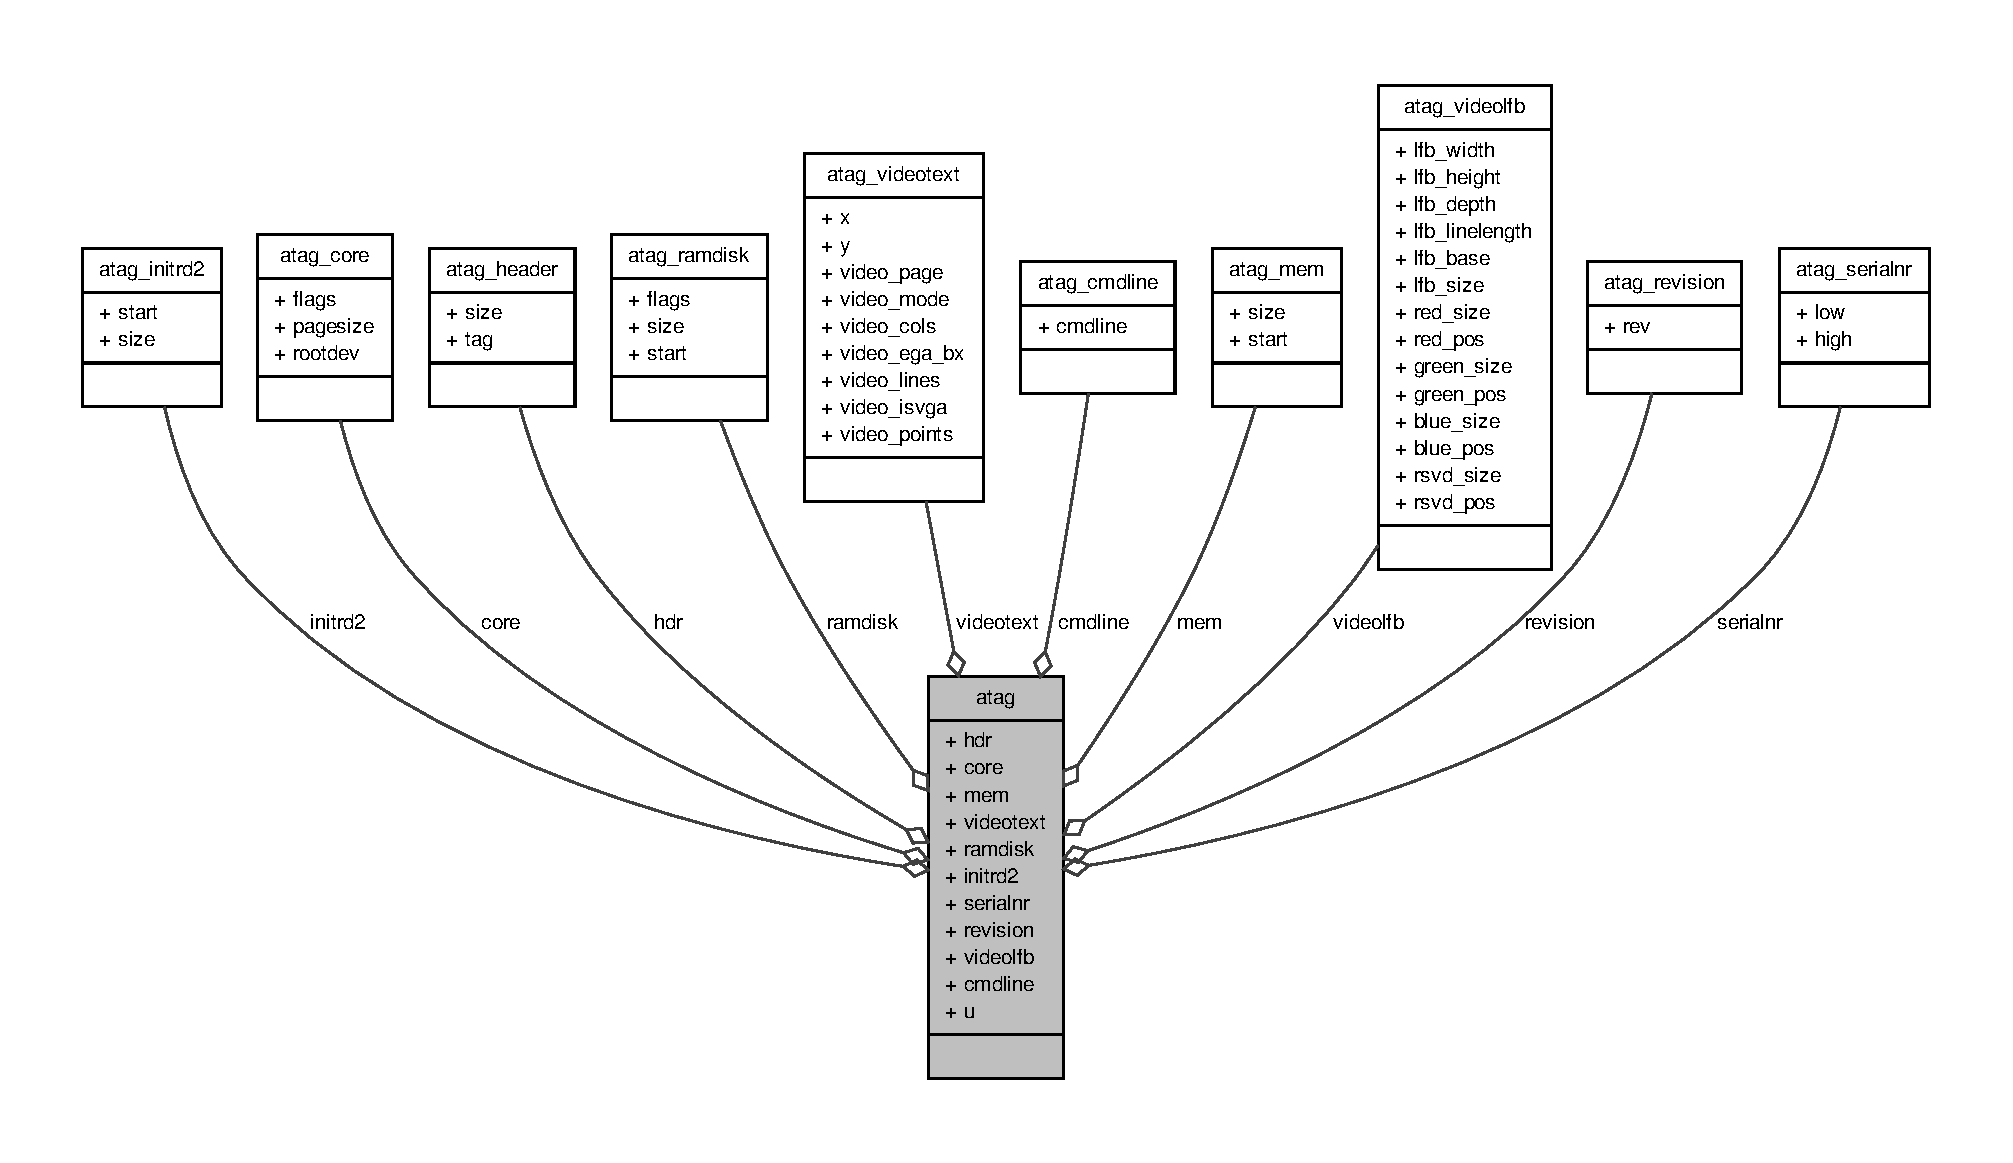
\includegraphics[width=350pt]{structatag__coll__graph}
\end{center}
\end{figure}
\subsection*{\-Data \-Fields}
\begin{DoxyCompactItemize}
\item 
struct \hyperlink{structatag__header}{atag\-\_\-header} \hyperlink{structatag_a66c7c965cacca4dc92877044e8dfe41b}{hdr}
\item 
\begin{tabbing}
xx\=xx\=xx\=xx\=xx\=xx\=xx\=xx\=xx\=\kill
union \{\\
\>struct \hyperlink{structatag__core}{atag\_core} \hyperlink{structatag_a3e5111a292381fc207b3a8641ec6768b}{core}\\
\>struct \hyperlink{structatag__mem}{atag\_mem} \hyperlink{structatag_a0aba8dc5f020043ea2cb77d6881db48c}{mem}\\
\>struct \hyperlink{structatag__videotext}{atag\_videotext} \hyperlink{structatag_a7ad6fedc71b884606da461f8c80aed71}{videotext}\\
\>struct \hyperlink{structatag__ramdisk}{atag\_ramdisk} \hyperlink{structatag_a376ebff53c0bc342459800dcbe5143db}{ramdisk}\\
\>struct \hyperlink{structatag__initrd2}{atag\_initrd2} \hyperlink{structatag_a0b791b85cd154b77c27383a8fe75d6e9}{initrd2}\\
\>struct \hyperlink{structatag__serialnr}{atag\_serialnr} \hyperlink{structatag_ac9d79c3e0dfd42492b63d91cf99a39c2}{serialnr}\\
\>struct \hyperlink{structatag__revision}{atag\_revision} \hyperlink{structatag_ad9f0972cb9739fe2952313cfb7086209}{revision}\\
\>struct \hyperlink{structatag__videolfb}{atag\_videolfb} \hyperlink{structatag_acb9829613674a77c810583283cf73210}{videolfb}\\
\>struct \hyperlink{structatag__cmdline}{atag\_cmdline} \hyperlink{structatag_a967131921bcaf65942ba3c162ca9b216}{cmdline}\\
\} \hyperlink{structatag_aacb06f1a4723ee6a39bd41e95aecd225}{u}\\

\end{tabbing}\end{DoxyCompactItemize}


\subsection{\-Detailed \-Description}


\-Definition at line 83 of file loadlinux.\-c.



\subsection{\-Field \-Documentation}
\hypertarget{structatag_a967131921bcaf65942ba3c162ca9b216}{\index{atag@{atag}!cmdline@{cmdline}}
\index{cmdline@{cmdline}!atag@{atag}}
\subsubsection[{cmdline}]{\setlength{\rightskip}{0pt plus 5cm}struct {\bf atag\-\_\-cmdline} {\bf cmdline}}}\label{structatag_a967131921bcaf65942ba3c162ca9b216}


\-Definition at line 94 of file loadlinux.\-c.

\hypertarget{structatag_a3e5111a292381fc207b3a8641ec6768b}{\index{atag@{atag}!core@{core}}
\index{core@{core}!atag@{atag}}
\subsubsection[{core}]{\setlength{\rightskip}{0pt plus 5cm}struct {\bf atag\-\_\-core} {\bf core}}}\label{structatag_a3e5111a292381fc207b3a8641ec6768b}


\-Definition at line 86 of file loadlinux.\-c.

\hypertarget{structatag_a66c7c965cacca4dc92877044e8dfe41b}{\index{atag@{atag}!hdr@{hdr}}
\index{hdr@{hdr}!atag@{atag}}
\subsubsection[{hdr}]{\setlength{\rightskip}{0pt plus 5cm}struct {\bf atag\-\_\-header} {\bf hdr}}}\label{structatag_a66c7c965cacca4dc92877044e8dfe41b}


\-Definition at line 84 of file loadlinux.\-c.

\hypertarget{structatag_a0b791b85cd154b77c27383a8fe75d6e9}{\index{atag@{atag}!initrd2@{initrd2}}
\index{initrd2@{initrd2}!atag@{atag}}
\subsubsection[{initrd2}]{\setlength{\rightskip}{0pt plus 5cm}struct {\bf atag\-\_\-initrd2} {\bf initrd2}}}\label{structatag_a0b791b85cd154b77c27383a8fe75d6e9}


\-Definition at line 90 of file loadlinux.\-c.

\hypertarget{structatag_a0aba8dc5f020043ea2cb77d6881db48c}{\index{atag@{atag}!mem@{mem}}
\index{mem@{mem}!atag@{atag}}
\subsubsection[{mem}]{\setlength{\rightskip}{0pt plus 5cm}struct {\bf atag\-\_\-mem} {\bf mem}}}\label{structatag_a0aba8dc5f020043ea2cb77d6881db48c}


\-Definition at line 87 of file loadlinux.\-c.

\hypertarget{structatag_a376ebff53c0bc342459800dcbe5143db}{\index{atag@{atag}!ramdisk@{ramdisk}}
\index{ramdisk@{ramdisk}!atag@{atag}}
\subsubsection[{ramdisk}]{\setlength{\rightskip}{0pt plus 5cm}struct {\bf atag\-\_\-ramdisk} {\bf ramdisk}}}\label{structatag_a376ebff53c0bc342459800dcbe5143db}


\-Definition at line 89 of file loadlinux.\-c.

\hypertarget{structatag_ad9f0972cb9739fe2952313cfb7086209}{\index{atag@{atag}!revision@{revision}}
\index{revision@{revision}!atag@{atag}}
\subsubsection[{revision}]{\setlength{\rightskip}{0pt plus 5cm}struct {\bf atag\-\_\-revision} {\bf revision}}}\label{structatag_ad9f0972cb9739fe2952313cfb7086209}


\-Definition at line 92 of file loadlinux.\-c.

\hypertarget{structatag_ac9d79c3e0dfd42492b63d91cf99a39c2}{\index{atag@{atag}!serialnr@{serialnr}}
\index{serialnr@{serialnr}!atag@{atag}}
\subsubsection[{serialnr}]{\setlength{\rightskip}{0pt plus 5cm}struct {\bf atag\-\_\-serialnr} {\bf serialnr}}}\label{structatag_ac9d79c3e0dfd42492b63d91cf99a39c2}


\-Definition at line 91 of file loadlinux.\-c.

\hypertarget{structatag_aacb06f1a4723ee6a39bd41e95aecd225}{\index{atag@{atag}!u@{u}}
\index{u@{u}!atag@{atag}}
\subsubsection[{u}]{\setlength{\rightskip}{0pt plus 5cm}union \{ ... \}   {\bf u}}}\label{structatag_aacb06f1a4723ee6a39bd41e95aecd225}
\hypertarget{structatag_acb9829613674a77c810583283cf73210}{\index{atag@{atag}!videolfb@{videolfb}}
\index{videolfb@{videolfb}!atag@{atag}}
\subsubsection[{videolfb}]{\setlength{\rightskip}{0pt plus 5cm}struct {\bf atag\-\_\-videolfb} {\bf videolfb}}}\label{structatag_acb9829613674a77c810583283cf73210}


\-Definition at line 93 of file loadlinux.\-c.

\hypertarget{structatag_a7ad6fedc71b884606da461f8c80aed71}{\index{atag@{atag}!videotext@{videotext}}
\index{videotext@{videotext}!atag@{atag}}
\subsubsection[{videotext}]{\setlength{\rightskip}{0pt plus 5cm}struct {\bf atag\-\_\-videotext} {\bf videotext}}}\label{structatag_a7ad6fedc71b884606da461f8c80aed71}


\-Definition at line 88 of file loadlinux.\-c.



\-The documentation for this struct was generated from the following file\-:\begin{DoxyCompactItemize}
\item 
\hyperlink{loadlinux_8c}{loadlinux.\-c}\end{DoxyCompactItemize}

\hypertarget{structatag__cmdline}{\section{atag\-\_\-cmdline \-Struct \-Reference}
\label{structatag__cmdline}\index{atag\-\_\-cmdline@{atag\-\_\-cmdline}}
}
\subsection*{\-Data \-Fields}
\begin{DoxyCompactItemize}
\item 
char \hyperlink{structatag__cmdline_af65a749b1baeb0e29cd855abcac29905}{cmdline} \mbox{[}1\mbox{]}
\end{DoxyCompactItemize}


\subsection{\-Detailed \-Description}


\-Definition at line 44 of file loadlinux.\-c.



\subsection{\-Field \-Documentation}
\hypertarget{structatag__cmdline_af65a749b1baeb0e29cd855abcac29905}{\index{atag\-\_\-cmdline@{atag\-\_\-cmdline}!cmdline@{cmdline}}
\index{cmdline@{cmdline}!atag_cmdline@{atag\-\_\-cmdline}}
\subsubsection[{cmdline}]{\setlength{\rightskip}{0pt plus 5cm}char {\bf cmdline}\mbox{[}1\mbox{]}}}\label{structatag__cmdline_af65a749b1baeb0e29cd855abcac29905}


\-Definition at line 45 of file loadlinux.\-c.



\-The documentation for this struct was generated from the following file\-:\begin{DoxyCompactItemize}
\item 
\hyperlink{loadlinux_8c}{loadlinux.\-c}\end{DoxyCompactItemize}

\hypertarget{structatag__core}{\section{atag\-\_\-core \-Struct \-Reference}
\label{structatag__core}\index{atag\-\_\-core@{atag\-\_\-core}}
}
\subsection*{\-Data \-Fields}
\begin{DoxyCompactItemize}
\item 
\hyperlink{arch__types_8h_a435d1572bf3f880d55459d9805097f62}{uint32\-\_\-t} \hyperlink{structatag__core_a773b39d480759f67926cb18ae2219281}{flags}
\item 
\hyperlink{arch__types_8h_a435d1572bf3f880d55459d9805097f62}{uint32\-\_\-t} \hyperlink{structatag__core_a64a0f9cfdfcb358f8c69a1fa4ddd4742}{pagesize}
\item 
\hyperlink{arch__types_8h_a435d1572bf3f880d55459d9805097f62}{uint32\-\_\-t} \hyperlink{structatag__core_a79dc316159f961edcc34cc3a22db5260}{rootdev}
\end{DoxyCompactItemize}


\subsection{\-Detailed \-Description}


\-Definition at line 26 of file loadlinux.\-c.



\subsection{\-Field \-Documentation}
\hypertarget{structatag__core_a773b39d480759f67926cb18ae2219281}{\index{atag\-\_\-core@{atag\-\_\-core}!flags@{flags}}
\index{flags@{flags}!atag_core@{atag\-\_\-core}}
\subsubsection[{flags}]{\setlength{\rightskip}{0pt plus 5cm}{\bf uint32\-\_\-t} {\bf flags}}}\label{structatag__core_a773b39d480759f67926cb18ae2219281}


\-Definition at line 27 of file loadlinux.\-c.

\hypertarget{structatag__core_a64a0f9cfdfcb358f8c69a1fa4ddd4742}{\index{atag\-\_\-core@{atag\-\_\-core}!pagesize@{pagesize}}
\index{pagesize@{pagesize}!atag_core@{atag\-\_\-core}}
\subsubsection[{pagesize}]{\setlength{\rightskip}{0pt plus 5cm}{\bf uint32\-\_\-t} {\bf pagesize}}}\label{structatag__core_a64a0f9cfdfcb358f8c69a1fa4ddd4742}


\-Definition at line 28 of file loadlinux.\-c.

\hypertarget{structatag__core_a79dc316159f961edcc34cc3a22db5260}{\index{atag\-\_\-core@{atag\-\_\-core}!rootdev@{rootdev}}
\index{rootdev@{rootdev}!atag_core@{atag\-\_\-core}}
\subsubsection[{rootdev}]{\setlength{\rightskip}{0pt plus 5cm}{\bf uint32\-\_\-t} {\bf rootdev}}}\label{structatag__core_a79dc316159f961edcc34cc3a22db5260}


\-Definition at line 29 of file loadlinux.\-c.



\-The documentation for this struct was generated from the following file\-:\begin{DoxyCompactItemize}
\item 
\hyperlink{loadlinux_8c}{loadlinux.\-c}\end{DoxyCompactItemize}

\hypertarget{structatag__header}{\section{atag\-\_\-header \-Struct \-Reference}
\label{structatag__header}\index{atag\-\_\-header@{atag\-\_\-header}}
}
\subsection*{\-Data \-Fields}
\begin{DoxyCompactItemize}
\item 
\hyperlink{arch__types_8h_a435d1572bf3f880d55459d9805097f62}{uint32\-\_\-t} \hyperlink{structatag__header_ab2c6b258f02add8fdf4cfc7c371dd772}{size}
\item 
\hyperlink{arch__types_8h_a435d1572bf3f880d55459d9805097f62}{uint32\-\_\-t} \hyperlink{structatag__header_a1c50fcd1195659821729f52af8f3bb7d}{tag}
\end{DoxyCompactItemize}


\subsection{\-Detailed \-Description}


\-Definition at line 22 of file loadlinux.\-c.



\subsection{\-Field \-Documentation}
\hypertarget{structatag__header_ab2c6b258f02add8fdf4cfc7c371dd772}{\index{atag\-\_\-header@{atag\-\_\-header}!size@{size}}
\index{size@{size}!atag_header@{atag\-\_\-header}}
\subsubsection[{size}]{\setlength{\rightskip}{0pt plus 5cm}{\bf uint32\-\_\-t} {\bf size}}}\label{structatag__header_ab2c6b258f02add8fdf4cfc7c371dd772}


\-Definition at line 23 of file loadlinux.\-c.

\hypertarget{structatag__header_a1c50fcd1195659821729f52af8f3bb7d}{\index{atag\-\_\-header@{atag\-\_\-header}!tag@{tag}}
\index{tag@{tag}!atag_header@{atag\-\_\-header}}
\subsubsection[{tag}]{\setlength{\rightskip}{0pt plus 5cm}{\bf uint32\-\_\-t} {\bf tag}}}\label{structatag__header_a1c50fcd1195659821729f52af8f3bb7d}


\-Definition at line 24 of file loadlinux.\-c.



\-The documentation for this struct was generated from the following file\-:\begin{DoxyCompactItemize}
\item 
\hyperlink{loadlinux_8c}{loadlinux.\-c}\end{DoxyCompactItemize}

\hypertarget{structatag__initrd2}{\section{atag\-\_\-initrd2 \-Struct \-Reference}
\label{structatag__initrd2}\index{atag\-\_\-initrd2@{atag\-\_\-initrd2}}
}
\subsection*{\-Data \-Fields}
\begin{DoxyCompactItemize}
\item 
\hyperlink{arch__types_8h_a435d1572bf3f880d55459d9805097f62}{uint32\-\_\-t} \hyperlink{structatag__initrd2_a61eb63d26b2fa6c2971603ceccffb14b}{start}
\item 
\hyperlink{arch__types_8h_a435d1572bf3f880d55459d9805097f62}{uint32\-\_\-t} \hyperlink{structatag__initrd2_ab2c6b258f02add8fdf4cfc7c371dd772}{size}
\end{DoxyCompactItemize}


\subsection{\-Detailed \-Description}


\-Definition at line 63 of file loadlinux.\-c.



\subsection{\-Field \-Documentation}
\hypertarget{structatag__initrd2_ab2c6b258f02add8fdf4cfc7c371dd772}{\index{atag\-\_\-initrd2@{atag\-\_\-initrd2}!size@{size}}
\index{size@{size}!atag_initrd2@{atag\-\_\-initrd2}}
\subsubsection[{size}]{\setlength{\rightskip}{0pt plus 5cm}{\bf uint32\-\_\-t} {\bf size}}}\label{structatag__initrd2_ab2c6b258f02add8fdf4cfc7c371dd772}


\-Definition at line 65 of file loadlinux.\-c.

\hypertarget{structatag__initrd2_a61eb63d26b2fa6c2971603ceccffb14b}{\index{atag\-\_\-initrd2@{atag\-\_\-initrd2}!start@{start}}
\index{start@{start}!atag_initrd2@{atag\-\_\-initrd2}}
\subsubsection[{start}]{\setlength{\rightskip}{0pt plus 5cm}{\bf uint32\-\_\-t} {\bf start}}}\label{structatag__initrd2_a61eb63d26b2fa6c2971603ceccffb14b}


\-Definition at line 64 of file loadlinux.\-c.



\-The documentation for this struct was generated from the following file\-:\begin{DoxyCompactItemize}
\item 
\hyperlink{loadlinux_8c}{loadlinux.\-c}\end{DoxyCompactItemize}

\hypertarget{structatag__mem}{\section{atag\-\_\-mem \-Struct \-Reference}
\label{structatag__mem}\index{atag\-\_\-mem@{atag\-\_\-mem}}
}
\subsection*{\-Data \-Fields}
\begin{DoxyCompactItemize}
\item 
\hyperlink{arch__types_8h_a435d1572bf3f880d55459d9805097f62}{uint32\-\_\-t} \hyperlink{structatag__mem_ab2c6b258f02add8fdf4cfc7c371dd772}{size}
\item 
\hyperlink{arch__types_8h_a435d1572bf3f880d55459d9805097f62}{uint32\-\_\-t} \hyperlink{structatag__mem_a61eb63d26b2fa6c2971603ceccffb14b}{start}
\end{DoxyCompactItemize}


\subsection{\-Detailed \-Description}


\-Definition at line 32 of file loadlinux.\-c.



\subsection{\-Field \-Documentation}
\hypertarget{structatag__mem_ab2c6b258f02add8fdf4cfc7c371dd772}{\index{atag\-\_\-mem@{atag\-\_\-mem}!size@{size}}
\index{size@{size}!atag_mem@{atag\-\_\-mem}}
\subsubsection[{size}]{\setlength{\rightskip}{0pt plus 5cm}{\bf uint32\-\_\-t} {\bf size}}}\label{structatag__mem_ab2c6b258f02add8fdf4cfc7c371dd772}


\-Definition at line 33 of file loadlinux.\-c.

\hypertarget{structatag__mem_a61eb63d26b2fa6c2971603ceccffb14b}{\index{atag\-\_\-mem@{atag\-\_\-mem}!start@{start}}
\index{start@{start}!atag_mem@{atag\-\_\-mem}}
\subsubsection[{start}]{\setlength{\rightskip}{0pt plus 5cm}{\bf uint32\-\_\-t} {\bf start}}}\label{structatag__mem_a61eb63d26b2fa6c2971603ceccffb14b}


\-Definition at line 34 of file loadlinux.\-c.



\-The documentation for this struct was generated from the following file\-:\begin{DoxyCompactItemize}
\item 
\hyperlink{loadlinux_8c}{loadlinux.\-c}\end{DoxyCompactItemize}

\hypertarget{structatag__ramdisk}{\section{atag\-\_\-ramdisk \-Struct \-Reference}
\label{structatag__ramdisk}\index{atag\-\_\-ramdisk@{atag\-\_\-ramdisk}}
}
\subsection*{\-Data \-Fields}
\begin{DoxyCompactItemize}
\item 
\hyperlink{arch__types_8h_a435d1572bf3f880d55459d9805097f62}{uint32\-\_\-t} \hyperlink{structatag__ramdisk_a773b39d480759f67926cb18ae2219281}{flags}
\item 
\hyperlink{arch__types_8h_a435d1572bf3f880d55459d9805097f62}{uint32\-\_\-t} \hyperlink{structatag__ramdisk_ab2c6b258f02add8fdf4cfc7c371dd772}{size}
\item 
\hyperlink{arch__types_8h_a435d1572bf3f880d55459d9805097f62}{uint32\-\_\-t} \hyperlink{structatag__ramdisk_a61eb63d26b2fa6c2971603ceccffb14b}{start}
\end{DoxyCompactItemize}


\subsection{\-Detailed \-Description}


\-Definition at line 47 of file loadlinux.\-c.



\subsection{\-Field \-Documentation}
\hypertarget{structatag__ramdisk_a773b39d480759f67926cb18ae2219281}{\index{atag\-\_\-ramdisk@{atag\-\_\-ramdisk}!flags@{flags}}
\index{flags@{flags}!atag_ramdisk@{atag\-\_\-ramdisk}}
\subsubsection[{flags}]{\setlength{\rightskip}{0pt plus 5cm}{\bf uint32\-\_\-t} {\bf flags}}}\label{structatag__ramdisk_a773b39d480759f67926cb18ae2219281}


\-Definition at line 48 of file loadlinux.\-c.

\hypertarget{structatag__ramdisk_ab2c6b258f02add8fdf4cfc7c371dd772}{\index{atag\-\_\-ramdisk@{atag\-\_\-ramdisk}!size@{size}}
\index{size@{size}!atag_ramdisk@{atag\-\_\-ramdisk}}
\subsubsection[{size}]{\setlength{\rightskip}{0pt plus 5cm}{\bf uint32\-\_\-t} {\bf size}}}\label{structatag__ramdisk_ab2c6b258f02add8fdf4cfc7c371dd772}


\-Definition at line 49 of file loadlinux.\-c.

\hypertarget{structatag__ramdisk_a61eb63d26b2fa6c2971603ceccffb14b}{\index{atag\-\_\-ramdisk@{atag\-\_\-ramdisk}!start@{start}}
\index{start@{start}!atag_ramdisk@{atag\-\_\-ramdisk}}
\subsubsection[{start}]{\setlength{\rightskip}{0pt plus 5cm}{\bf uint32\-\_\-t} {\bf start}}}\label{structatag__ramdisk_a61eb63d26b2fa6c2971603ceccffb14b}


\-Definition at line 50 of file loadlinux.\-c.



\-The documentation for this struct was generated from the following file\-:\begin{DoxyCompactItemize}
\item 
\hyperlink{loadlinux_8c}{loadlinux.\-c}\end{DoxyCompactItemize}

\hypertarget{structatag__revision}{\section{atag\-\_\-revision \-Struct \-Reference}
\label{structatag__revision}\index{atag\-\_\-revision@{atag\-\_\-revision}}
}
\subsection*{\-Data \-Fields}
\begin{DoxyCompactItemize}
\item 
\hyperlink{arch__types_8h_a435d1572bf3f880d55459d9805097f62}{uint32\-\_\-t} \hyperlink{structatag__revision_a9785d281d0ca6a77360f05a7d653a80f}{rev}
\end{DoxyCompactItemize}


\subsection{\-Detailed \-Description}


\-Definition at line 41 of file loadlinux.\-c.



\subsection{\-Field \-Documentation}
\hypertarget{structatag__revision_a9785d281d0ca6a77360f05a7d653a80f}{\index{atag\-\_\-revision@{atag\-\_\-revision}!rev@{rev}}
\index{rev@{rev}!atag_revision@{atag\-\_\-revision}}
\subsubsection[{rev}]{\setlength{\rightskip}{0pt plus 5cm}{\bf uint32\-\_\-t} {\bf rev}}}\label{structatag__revision_a9785d281d0ca6a77360f05a7d653a80f}


\-Definition at line 42 of file loadlinux.\-c.



\-The documentation for this struct was generated from the following file\-:\begin{DoxyCompactItemize}
\item 
\hyperlink{loadlinux_8c}{loadlinux.\-c}\end{DoxyCompactItemize}

\hypertarget{structatag__serialnr}{\section{atag\-\_\-serialnr \-Struct \-Reference}
\label{structatag__serialnr}\index{atag\-\_\-serialnr@{atag\-\_\-serialnr}}
}
\subsection*{\-Data \-Fields}
\begin{DoxyCompactItemize}
\item 
\hyperlink{arch__types_8h_a435d1572bf3f880d55459d9805097f62}{uint32\-\_\-t} \hyperlink{structatag__serialnr_a864f755b7008df85b29726891bdd4fbd}{low}
\item 
\hyperlink{arch__types_8h_a435d1572bf3f880d55459d9805097f62}{uint32\-\_\-t} \hyperlink{structatag__serialnr_a0d90a9fe74bca2dccde7f81cddfdf7b0}{high}
\end{DoxyCompactItemize}


\subsection{\-Detailed \-Description}


\-Definition at line 36 of file loadlinux.\-c.



\subsection{\-Field \-Documentation}
\hypertarget{structatag__serialnr_a0d90a9fe74bca2dccde7f81cddfdf7b0}{\index{atag\-\_\-serialnr@{atag\-\_\-serialnr}!high@{high}}
\index{high@{high}!atag_serialnr@{atag\-\_\-serialnr}}
\subsubsection[{high}]{\setlength{\rightskip}{0pt plus 5cm}{\bf uint32\-\_\-t} {\bf high}}}\label{structatag__serialnr_a0d90a9fe74bca2dccde7f81cddfdf7b0}


\-Definition at line 38 of file loadlinux.\-c.

\hypertarget{structatag__serialnr_a864f755b7008df85b29726891bdd4fbd}{\index{atag\-\_\-serialnr@{atag\-\_\-serialnr}!low@{low}}
\index{low@{low}!atag_serialnr@{atag\-\_\-serialnr}}
\subsubsection[{low}]{\setlength{\rightskip}{0pt plus 5cm}{\bf uint32\-\_\-t} {\bf low}}}\label{structatag__serialnr_a864f755b7008df85b29726891bdd4fbd}


\-Definition at line 37 of file loadlinux.\-c.



\-The documentation for this struct was generated from the following file\-:\begin{DoxyCompactItemize}
\item 
\hyperlink{loadlinux_8c}{loadlinux.\-c}\end{DoxyCompactItemize}

\hypertarget{structatag__videolfb}{\section{atag\-\_\-videolfb \-Struct \-Reference}
\label{structatag__videolfb}\index{atag\-\_\-videolfb@{atag\-\_\-videolfb}}
}
\subsection*{\-Data \-Fields}
\begin{DoxyCompactItemize}
\item 
\hyperlink{arch__types_8h_a273cf69d639a59973b6019625df33e30}{uint16\-\_\-t} \hyperlink{structatag__videolfb_ad9683bde4f1b9753114579a20f8b2ea6}{lfb\-\_\-width}
\item 
\hyperlink{arch__types_8h_a273cf69d639a59973b6019625df33e30}{uint16\-\_\-t} \hyperlink{structatag__videolfb_a6f3799e51d4a717803188027c594bb78}{lfb\-\_\-height}
\item 
\hyperlink{arch__types_8h_a273cf69d639a59973b6019625df33e30}{uint16\-\_\-t} \hyperlink{structatag__videolfb_a1e9d69114f74762a7cf07784f2bf54e1}{lfb\-\_\-depth}
\item 
\hyperlink{arch__types_8h_a273cf69d639a59973b6019625df33e30}{uint16\-\_\-t} \hyperlink{structatag__videolfb_a190b2b21aaf18f335c623ec415bf3bf2}{lfb\-\_\-linelength}
\item 
\hyperlink{arch__types_8h_a435d1572bf3f880d55459d9805097f62}{uint32\-\_\-t} \hyperlink{structatag__videolfb_a9271f1ecad08469fd6f7c70fcf639b28}{lfb\-\_\-base}
\item 
\hyperlink{arch__types_8h_a435d1572bf3f880d55459d9805097f62}{uint32\-\_\-t} \hyperlink{structatag__videolfb_afa0a0332b26a2414c29750b989c2bd99}{lfb\-\_\-size}
\item 
\hyperlink{arch__types_8h_aba7bc1797add20fe3efdf37ced1182c5}{uint8\-\_\-t} \hyperlink{structatag__videolfb_a466eb668b84c08bf28de034321c29241}{red\-\_\-size}
\item 
\hyperlink{arch__types_8h_aba7bc1797add20fe3efdf37ced1182c5}{uint8\-\_\-t} \hyperlink{structatag__videolfb_a7e871d12fa956ff686bf9d2d39788d70}{red\-\_\-pos}
\item 
\hyperlink{arch__types_8h_aba7bc1797add20fe3efdf37ced1182c5}{uint8\-\_\-t} \hyperlink{structatag__videolfb_a282829825c751f574c461ea4e2a21b81}{green\-\_\-size}
\item 
\hyperlink{arch__types_8h_aba7bc1797add20fe3efdf37ced1182c5}{uint8\-\_\-t} \hyperlink{structatag__videolfb_a298fca41fa1fd8bc98c232788ab7d47f}{green\-\_\-pos}
\item 
\hyperlink{arch__types_8h_aba7bc1797add20fe3efdf37ced1182c5}{uint8\-\_\-t} \hyperlink{structatag__videolfb_a4b0c692ff987aeedc4922031b972e45f}{blue\-\_\-size}
\item 
\hyperlink{arch__types_8h_aba7bc1797add20fe3efdf37ced1182c5}{uint8\-\_\-t} \hyperlink{structatag__videolfb_aec62dfb090ca6c08e0df6748193598e5}{blue\-\_\-pos}
\item 
\hyperlink{arch__types_8h_aba7bc1797add20fe3efdf37ced1182c5}{uint8\-\_\-t} \hyperlink{structatag__videolfb_a9d840fbd8d826b24ae26dededb556fa0}{rsvd\-\_\-size}
\item 
\hyperlink{arch__types_8h_aba7bc1797add20fe3efdf37ced1182c5}{uint8\-\_\-t} \hyperlink{structatag__videolfb_a631ed037a09490663fbd27eb4224fc47}{rsvd\-\_\-pos}
\end{DoxyCompactItemize}


\subsection{\-Detailed \-Description}


\-Definition at line 67 of file loadlinux.\-c.



\subsection{\-Field \-Documentation}
\hypertarget{structatag__videolfb_aec62dfb090ca6c08e0df6748193598e5}{\index{atag\-\_\-videolfb@{atag\-\_\-videolfb}!blue\-\_\-pos@{blue\-\_\-pos}}
\index{blue\-\_\-pos@{blue\-\_\-pos}!atag_videolfb@{atag\-\_\-videolfb}}
\subsubsection[{blue\-\_\-pos}]{\setlength{\rightskip}{0pt plus 5cm}{\bf uint8\-\_\-t} {\bf blue\-\_\-pos}}}\label{structatag__videolfb_aec62dfb090ca6c08e0df6748193598e5}


\-Definition at line 79 of file loadlinux.\-c.

\hypertarget{structatag__videolfb_a4b0c692ff987aeedc4922031b972e45f}{\index{atag\-\_\-videolfb@{atag\-\_\-videolfb}!blue\-\_\-size@{blue\-\_\-size}}
\index{blue\-\_\-size@{blue\-\_\-size}!atag_videolfb@{atag\-\_\-videolfb}}
\subsubsection[{blue\-\_\-size}]{\setlength{\rightskip}{0pt plus 5cm}{\bf uint8\-\_\-t} {\bf blue\-\_\-size}}}\label{structatag__videolfb_a4b0c692ff987aeedc4922031b972e45f}


\-Definition at line 78 of file loadlinux.\-c.

\hypertarget{structatag__videolfb_a298fca41fa1fd8bc98c232788ab7d47f}{\index{atag\-\_\-videolfb@{atag\-\_\-videolfb}!green\-\_\-pos@{green\-\_\-pos}}
\index{green\-\_\-pos@{green\-\_\-pos}!atag_videolfb@{atag\-\_\-videolfb}}
\subsubsection[{green\-\_\-pos}]{\setlength{\rightskip}{0pt plus 5cm}{\bf uint8\-\_\-t} {\bf green\-\_\-pos}}}\label{structatag__videolfb_a298fca41fa1fd8bc98c232788ab7d47f}


\-Definition at line 77 of file loadlinux.\-c.

\hypertarget{structatag__videolfb_a282829825c751f574c461ea4e2a21b81}{\index{atag\-\_\-videolfb@{atag\-\_\-videolfb}!green\-\_\-size@{green\-\_\-size}}
\index{green\-\_\-size@{green\-\_\-size}!atag_videolfb@{atag\-\_\-videolfb}}
\subsubsection[{green\-\_\-size}]{\setlength{\rightskip}{0pt plus 5cm}{\bf uint8\-\_\-t} {\bf green\-\_\-size}}}\label{structatag__videolfb_a282829825c751f574c461ea4e2a21b81}


\-Definition at line 76 of file loadlinux.\-c.

\hypertarget{structatag__videolfb_a9271f1ecad08469fd6f7c70fcf639b28}{\index{atag\-\_\-videolfb@{atag\-\_\-videolfb}!lfb\-\_\-base@{lfb\-\_\-base}}
\index{lfb\-\_\-base@{lfb\-\_\-base}!atag_videolfb@{atag\-\_\-videolfb}}
\subsubsection[{lfb\-\_\-base}]{\setlength{\rightskip}{0pt plus 5cm}{\bf uint32\-\_\-t} {\bf lfb\-\_\-base}}}\label{structatag__videolfb_a9271f1ecad08469fd6f7c70fcf639b28}


\-Definition at line 72 of file loadlinux.\-c.

\hypertarget{structatag__videolfb_a1e9d69114f74762a7cf07784f2bf54e1}{\index{atag\-\_\-videolfb@{atag\-\_\-videolfb}!lfb\-\_\-depth@{lfb\-\_\-depth}}
\index{lfb\-\_\-depth@{lfb\-\_\-depth}!atag_videolfb@{atag\-\_\-videolfb}}
\subsubsection[{lfb\-\_\-depth}]{\setlength{\rightskip}{0pt plus 5cm}{\bf uint16\-\_\-t} {\bf lfb\-\_\-depth}}}\label{structatag__videolfb_a1e9d69114f74762a7cf07784f2bf54e1}


\-Definition at line 70 of file loadlinux.\-c.

\hypertarget{structatag__videolfb_a6f3799e51d4a717803188027c594bb78}{\index{atag\-\_\-videolfb@{atag\-\_\-videolfb}!lfb\-\_\-height@{lfb\-\_\-height}}
\index{lfb\-\_\-height@{lfb\-\_\-height}!atag_videolfb@{atag\-\_\-videolfb}}
\subsubsection[{lfb\-\_\-height}]{\setlength{\rightskip}{0pt plus 5cm}{\bf uint16\-\_\-t} {\bf lfb\-\_\-height}}}\label{structatag__videolfb_a6f3799e51d4a717803188027c594bb78}


\-Definition at line 69 of file loadlinux.\-c.

\hypertarget{structatag__videolfb_a190b2b21aaf18f335c623ec415bf3bf2}{\index{atag\-\_\-videolfb@{atag\-\_\-videolfb}!lfb\-\_\-linelength@{lfb\-\_\-linelength}}
\index{lfb\-\_\-linelength@{lfb\-\_\-linelength}!atag_videolfb@{atag\-\_\-videolfb}}
\subsubsection[{lfb\-\_\-linelength}]{\setlength{\rightskip}{0pt plus 5cm}{\bf uint16\-\_\-t} {\bf lfb\-\_\-linelength}}}\label{structatag__videolfb_a190b2b21aaf18f335c623ec415bf3bf2}


\-Definition at line 71 of file loadlinux.\-c.

\hypertarget{structatag__videolfb_afa0a0332b26a2414c29750b989c2bd99}{\index{atag\-\_\-videolfb@{atag\-\_\-videolfb}!lfb\-\_\-size@{lfb\-\_\-size}}
\index{lfb\-\_\-size@{lfb\-\_\-size}!atag_videolfb@{atag\-\_\-videolfb}}
\subsubsection[{lfb\-\_\-size}]{\setlength{\rightskip}{0pt plus 5cm}{\bf uint32\-\_\-t} {\bf lfb\-\_\-size}}}\label{structatag__videolfb_afa0a0332b26a2414c29750b989c2bd99}


\-Definition at line 73 of file loadlinux.\-c.

\hypertarget{structatag__videolfb_ad9683bde4f1b9753114579a20f8b2ea6}{\index{atag\-\_\-videolfb@{atag\-\_\-videolfb}!lfb\-\_\-width@{lfb\-\_\-width}}
\index{lfb\-\_\-width@{lfb\-\_\-width}!atag_videolfb@{atag\-\_\-videolfb}}
\subsubsection[{lfb\-\_\-width}]{\setlength{\rightskip}{0pt plus 5cm}{\bf uint16\-\_\-t} {\bf lfb\-\_\-width}}}\label{structatag__videolfb_ad9683bde4f1b9753114579a20f8b2ea6}


\-Definition at line 68 of file loadlinux.\-c.

\hypertarget{structatag__videolfb_a7e871d12fa956ff686bf9d2d39788d70}{\index{atag\-\_\-videolfb@{atag\-\_\-videolfb}!red\-\_\-pos@{red\-\_\-pos}}
\index{red\-\_\-pos@{red\-\_\-pos}!atag_videolfb@{atag\-\_\-videolfb}}
\subsubsection[{red\-\_\-pos}]{\setlength{\rightskip}{0pt plus 5cm}{\bf uint8\-\_\-t} {\bf red\-\_\-pos}}}\label{structatag__videolfb_a7e871d12fa956ff686bf9d2d39788d70}


\-Definition at line 75 of file loadlinux.\-c.

\hypertarget{structatag__videolfb_a466eb668b84c08bf28de034321c29241}{\index{atag\-\_\-videolfb@{atag\-\_\-videolfb}!red\-\_\-size@{red\-\_\-size}}
\index{red\-\_\-size@{red\-\_\-size}!atag_videolfb@{atag\-\_\-videolfb}}
\subsubsection[{red\-\_\-size}]{\setlength{\rightskip}{0pt plus 5cm}{\bf uint8\-\_\-t} {\bf red\-\_\-size}}}\label{structatag__videolfb_a466eb668b84c08bf28de034321c29241}


\-Definition at line 74 of file loadlinux.\-c.

\hypertarget{structatag__videolfb_a631ed037a09490663fbd27eb4224fc47}{\index{atag\-\_\-videolfb@{atag\-\_\-videolfb}!rsvd\-\_\-pos@{rsvd\-\_\-pos}}
\index{rsvd\-\_\-pos@{rsvd\-\_\-pos}!atag_videolfb@{atag\-\_\-videolfb}}
\subsubsection[{rsvd\-\_\-pos}]{\setlength{\rightskip}{0pt plus 5cm}{\bf uint8\-\_\-t} {\bf rsvd\-\_\-pos}}}\label{structatag__videolfb_a631ed037a09490663fbd27eb4224fc47}


\-Definition at line 81 of file loadlinux.\-c.

\hypertarget{structatag__videolfb_a9d840fbd8d826b24ae26dededb556fa0}{\index{atag\-\_\-videolfb@{atag\-\_\-videolfb}!rsvd\-\_\-size@{rsvd\-\_\-size}}
\index{rsvd\-\_\-size@{rsvd\-\_\-size}!atag_videolfb@{atag\-\_\-videolfb}}
\subsubsection[{rsvd\-\_\-size}]{\setlength{\rightskip}{0pt plus 5cm}{\bf uint8\-\_\-t} {\bf rsvd\-\_\-size}}}\label{structatag__videolfb_a9d840fbd8d826b24ae26dededb556fa0}


\-Definition at line 80 of file loadlinux.\-c.



\-The documentation for this struct was generated from the following file\-:\begin{DoxyCompactItemize}
\item 
\hyperlink{loadlinux_8c}{loadlinux.\-c}\end{DoxyCompactItemize}

\hypertarget{structatag__videotext}{\section{atag\-\_\-videotext \-Struct \-Reference}
\label{structatag__videotext}\index{atag\-\_\-videotext@{atag\-\_\-videotext}}
}
\subsection*{\-Data \-Fields}
\begin{DoxyCompactItemize}
\item 
\hyperlink{arch__types_8h_aba7bc1797add20fe3efdf37ced1182c5}{uint8\-\_\-t} \hyperlink{structatag__videotext_a0f561e77fa0f040b637f4e04f6cd8078}{x}
\item 
\hyperlink{arch__types_8h_aba7bc1797add20fe3efdf37ced1182c5}{uint8\-\_\-t} \hyperlink{structatag__videotext_a17f97f62d93bc8cfb4a2b5d273a2aa72}{y}
\item 
\hyperlink{arch__types_8h_a273cf69d639a59973b6019625df33e30}{uint16\-\_\-t} \hyperlink{structatag__videotext_ac6354ba51fe0fff7ac457ff0e4bf7c68}{video\-\_\-page}
\item 
\hyperlink{arch__types_8h_aba7bc1797add20fe3efdf37ced1182c5}{uint8\-\_\-t} \hyperlink{structatag__videotext_a1180b6b69ea36c4403ecfac38a3325db}{video\-\_\-mode}
\item 
\hyperlink{arch__types_8h_aba7bc1797add20fe3efdf37ced1182c5}{uint8\-\_\-t} \hyperlink{structatag__videotext_abd7a24d04c2e3a051bd316e44d025bbd}{video\-\_\-cols}
\item 
\hyperlink{arch__types_8h_a273cf69d639a59973b6019625df33e30}{uint16\-\_\-t} \hyperlink{structatag__videotext_a4fd68ac4ef39d5a73df67c42479b7380}{video\-\_\-ega\-\_\-bx}
\item 
\hyperlink{arch__types_8h_aba7bc1797add20fe3efdf37ced1182c5}{uint8\-\_\-t} \hyperlink{structatag__videotext_a63e3f823f9549fdb1ad1237f128afc56}{video\-\_\-lines}
\item 
\hyperlink{arch__types_8h_aba7bc1797add20fe3efdf37ced1182c5}{uint8\-\_\-t} \hyperlink{structatag__videotext_a8705641c3e6bd566573a2afe3bb66569}{video\-\_\-isvga}
\item 
\hyperlink{arch__types_8h_a273cf69d639a59973b6019625df33e30}{uint16\-\_\-t} \hyperlink{structatag__videotext_afe98e092bcb87124948444d17b59727b}{video\-\_\-points}
\end{DoxyCompactItemize}


\subsection{\-Detailed \-Description}


\-Definition at line 52 of file loadlinux.\-c.



\subsection{\-Field \-Documentation}
\hypertarget{structatag__videotext_abd7a24d04c2e3a051bd316e44d025bbd}{\index{atag\-\_\-videotext@{atag\-\_\-videotext}!video\-\_\-cols@{video\-\_\-cols}}
\index{video\-\_\-cols@{video\-\_\-cols}!atag_videotext@{atag\-\_\-videotext}}
\subsubsection[{video\-\_\-cols}]{\setlength{\rightskip}{0pt plus 5cm}{\bf uint8\-\_\-t} {\bf video\-\_\-cols}}}\label{structatag__videotext_abd7a24d04c2e3a051bd316e44d025bbd}


\-Definition at line 57 of file loadlinux.\-c.

\hypertarget{structatag__videotext_a4fd68ac4ef39d5a73df67c42479b7380}{\index{atag\-\_\-videotext@{atag\-\_\-videotext}!video\-\_\-ega\-\_\-bx@{video\-\_\-ega\-\_\-bx}}
\index{video\-\_\-ega\-\_\-bx@{video\-\_\-ega\-\_\-bx}!atag_videotext@{atag\-\_\-videotext}}
\subsubsection[{video\-\_\-ega\-\_\-bx}]{\setlength{\rightskip}{0pt plus 5cm}{\bf uint16\-\_\-t} {\bf video\-\_\-ega\-\_\-bx}}}\label{structatag__videotext_a4fd68ac4ef39d5a73df67c42479b7380}


\-Definition at line 58 of file loadlinux.\-c.

\hypertarget{structatag__videotext_a8705641c3e6bd566573a2afe3bb66569}{\index{atag\-\_\-videotext@{atag\-\_\-videotext}!video\-\_\-isvga@{video\-\_\-isvga}}
\index{video\-\_\-isvga@{video\-\_\-isvga}!atag_videotext@{atag\-\_\-videotext}}
\subsubsection[{video\-\_\-isvga}]{\setlength{\rightskip}{0pt plus 5cm}{\bf uint8\-\_\-t} {\bf video\-\_\-isvga}}}\label{structatag__videotext_a8705641c3e6bd566573a2afe3bb66569}


\-Definition at line 60 of file loadlinux.\-c.

\hypertarget{structatag__videotext_a63e3f823f9549fdb1ad1237f128afc56}{\index{atag\-\_\-videotext@{atag\-\_\-videotext}!video\-\_\-lines@{video\-\_\-lines}}
\index{video\-\_\-lines@{video\-\_\-lines}!atag_videotext@{atag\-\_\-videotext}}
\subsubsection[{video\-\_\-lines}]{\setlength{\rightskip}{0pt plus 5cm}{\bf uint8\-\_\-t} {\bf video\-\_\-lines}}}\label{structatag__videotext_a63e3f823f9549fdb1ad1237f128afc56}


\-Definition at line 59 of file loadlinux.\-c.

\hypertarget{structatag__videotext_a1180b6b69ea36c4403ecfac38a3325db}{\index{atag\-\_\-videotext@{atag\-\_\-videotext}!video\-\_\-mode@{video\-\_\-mode}}
\index{video\-\_\-mode@{video\-\_\-mode}!atag_videotext@{atag\-\_\-videotext}}
\subsubsection[{video\-\_\-mode}]{\setlength{\rightskip}{0pt plus 5cm}{\bf uint8\-\_\-t} {\bf video\-\_\-mode}}}\label{structatag__videotext_a1180b6b69ea36c4403ecfac38a3325db}


\-Definition at line 56 of file loadlinux.\-c.

\hypertarget{structatag__videotext_ac6354ba51fe0fff7ac457ff0e4bf7c68}{\index{atag\-\_\-videotext@{atag\-\_\-videotext}!video\-\_\-page@{video\-\_\-page}}
\index{video\-\_\-page@{video\-\_\-page}!atag_videotext@{atag\-\_\-videotext}}
\subsubsection[{video\-\_\-page}]{\setlength{\rightskip}{0pt plus 5cm}{\bf uint16\-\_\-t} {\bf video\-\_\-page}}}\label{structatag__videotext_ac6354ba51fe0fff7ac457ff0e4bf7c68}


\-Definition at line 55 of file loadlinux.\-c.

\hypertarget{structatag__videotext_afe98e092bcb87124948444d17b59727b}{\index{atag\-\_\-videotext@{atag\-\_\-videotext}!video\-\_\-points@{video\-\_\-points}}
\index{video\-\_\-points@{video\-\_\-points}!atag_videotext@{atag\-\_\-videotext}}
\subsubsection[{video\-\_\-points}]{\setlength{\rightskip}{0pt plus 5cm}{\bf uint16\-\_\-t} {\bf video\-\_\-points}}}\label{structatag__videotext_afe98e092bcb87124948444d17b59727b}


\-Definition at line 61 of file loadlinux.\-c.

\hypertarget{structatag__videotext_a0f561e77fa0f040b637f4e04f6cd8078}{\index{atag\-\_\-videotext@{atag\-\_\-videotext}!x@{x}}
\index{x@{x}!atag_videotext@{atag\-\_\-videotext}}
\subsubsection[{x}]{\setlength{\rightskip}{0pt plus 5cm}{\bf uint8\-\_\-t} {\bf x}}}\label{structatag__videotext_a0f561e77fa0f040b637f4e04f6cd8078}


\-Definition at line 53 of file loadlinux.\-c.

\hypertarget{structatag__videotext_a17f97f62d93bc8cfb4a2b5d273a2aa72}{\index{atag\-\_\-videotext@{atag\-\_\-videotext}!y@{y}}
\index{y@{y}!atag_videotext@{atag\-\_\-videotext}}
\subsubsection[{y}]{\setlength{\rightskip}{0pt plus 5cm}{\bf uint8\-\_\-t} {\bf y}}}\label{structatag__videotext_a17f97f62d93bc8cfb4a2b5d273a2aa72}


\-Definition at line 54 of file loadlinux.\-c.



\-The documentation for this struct was generated from the following file\-:\begin{DoxyCompactItemize}
\item 
\hyperlink{loadlinux_8c}{loadlinux.\-c}\end{DoxyCompactItemize}

\hypertarget{structgic}{\section{gic \-Struct \-Reference}
\label{structgic}\index{gic@{gic}}
}
\subsection*{\-Data \-Fields}
\begin{DoxyCompactItemize}
\item 
\hyperlink{arch__types_8h_a435d1572bf3f880d55459d9805097f62}{uint32\-\_\-t} \hyperlink{structgic_ab15249e04d1bee1b0997011912a87cbf}{baseaddr}
\item 
volatile \hyperlink{arch__types_8h_a435d1572bf3f880d55459d9805097f62}{uint32\-\_\-t} $\ast$ \hyperlink{structgic_a186421525f3bd36a65216cfdc79ce10e}{ba\-\_\-gicd}
\item 
volatile \hyperlink{arch__types_8h_a435d1572bf3f880d55459d9805097f62}{uint32\-\_\-t} $\ast$ \hyperlink{structgic_a83c305aab314213445ac83ad517e9be4}{ba\-\_\-gicc}
\item 
volatile \hyperlink{arch__types_8h_a435d1572bf3f880d55459d9805097f62}{uint32\-\_\-t} $\ast$ \hyperlink{structgic_aa93c957a17fef2d6779bde6b08f85050}{ba\-\_\-gich}
\item 
volatile \hyperlink{arch__types_8h_a435d1572bf3f880d55459d9805097f62}{uint32\-\_\-t} $\ast$ \hyperlink{structgic_acd803bc08a11a6e6222a8a156390599f}{ba\-\_\-gicv}
\item 
volatile \hyperlink{arch__types_8h_a435d1572bf3f880d55459d9805097f62}{uint32\-\_\-t} $\ast$ \hyperlink{structgic_a0dc2d2fdf039752758490aa59725fce2}{ba\-\_\-gicvi}
\item 
\hyperlink{arch__types_8h_a435d1572bf3f880d55459d9805097f62}{uint32\-\_\-t} \hyperlink{structgic_af6e49f2b9eca7c6ee734d83fdc035124}{lines}
\item 
\hyperlink{arch__types_8h_a435d1572bf3f880d55459d9805097f62}{uint32\-\_\-t} \hyperlink{structgic_a148b00861c88b4f5d5bf006071fbdc04}{cpus}
\item 
\hyperlink{gic_8h_a4b1f3150431142b6910f651a1172f446}{gic\-\_\-irq\-\_\-handler\-\_\-t} \hyperlink{structgic_a030df411878f4e7c744256f330692e95}{handlers} \mbox{[}\hyperlink{gic_8h_a1ae8d5cca4dfb10e3503d0acd68ea045}{\-G\-I\-C\-\_\-\-N\-U\-M\-\_\-\-M\-A\-X\-\_\-\-I\-R\-Q\-S}\mbox{]}
\item 
\hyperlink{arch__types_8h_a435d1572bf3f880d55459d9805097f62}{uint32\-\_\-t} \hyperlink{structgic_a874884c7efa14474f67d1a82b795ce3c}{initialized}
\end{DoxyCompactItemize}


\subsection{\-Detailed \-Description}


\-Definition at line 31 of file gic.\-c.



\subsection{\-Field \-Documentation}
\hypertarget{structgic_a83c305aab314213445ac83ad517e9be4}{\index{gic@{gic}!ba\-\_\-gicc@{ba\-\_\-gicc}}
\index{ba\-\_\-gicc@{ba\-\_\-gicc}!gic@{gic}}
\subsubsection[{ba\-\_\-gicc}]{\setlength{\rightskip}{0pt plus 5cm}volatile {\bf uint32\-\_\-t}$\ast$ {\bf ba\-\_\-gicc}}}\label{structgic_a83c305aab314213445ac83ad517e9be4}


\-Definition at line 34 of file gic.\-c.

\hypertarget{structgic_a186421525f3bd36a65216cfdc79ce10e}{\index{gic@{gic}!ba\-\_\-gicd@{ba\-\_\-gicd}}
\index{ba\-\_\-gicd@{ba\-\_\-gicd}!gic@{gic}}
\subsubsection[{ba\-\_\-gicd}]{\setlength{\rightskip}{0pt plus 5cm}volatile {\bf uint32\-\_\-t}$\ast$ {\bf ba\-\_\-gicd}}}\label{structgic_a186421525f3bd36a65216cfdc79ce10e}


\-Definition at line 33 of file gic.\-c.

\hypertarget{structgic_aa93c957a17fef2d6779bde6b08f85050}{\index{gic@{gic}!ba\-\_\-gich@{ba\-\_\-gich}}
\index{ba\-\_\-gich@{ba\-\_\-gich}!gic@{gic}}
\subsubsection[{ba\-\_\-gich}]{\setlength{\rightskip}{0pt plus 5cm}volatile {\bf uint32\-\_\-t}$\ast$ {\bf ba\-\_\-gich}}}\label{structgic_aa93c957a17fef2d6779bde6b08f85050}


\-Definition at line 35 of file gic.\-c.

\hypertarget{structgic_acd803bc08a11a6e6222a8a156390599f}{\index{gic@{gic}!ba\-\_\-gicv@{ba\-\_\-gicv}}
\index{ba\-\_\-gicv@{ba\-\_\-gicv}!gic@{gic}}
\subsubsection[{ba\-\_\-gicv}]{\setlength{\rightskip}{0pt plus 5cm}volatile {\bf uint32\-\_\-t}$\ast$ {\bf ba\-\_\-gicv}}}\label{structgic_acd803bc08a11a6e6222a8a156390599f}


\-Definition at line 36 of file gic.\-c.

\hypertarget{structgic_a0dc2d2fdf039752758490aa59725fce2}{\index{gic@{gic}!ba\-\_\-gicvi@{ba\-\_\-gicvi}}
\index{ba\-\_\-gicvi@{ba\-\_\-gicvi}!gic@{gic}}
\subsubsection[{ba\-\_\-gicvi}]{\setlength{\rightskip}{0pt plus 5cm}volatile {\bf uint32\-\_\-t}$\ast$ {\bf ba\-\_\-gicvi}}}\label{structgic_a0dc2d2fdf039752758490aa59725fce2}


\-Definition at line 37 of file gic.\-c.

\hypertarget{structgic_ab15249e04d1bee1b0997011912a87cbf}{\index{gic@{gic}!baseaddr@{baseaddr}}
\index{baseaddr@{baseaddr}!gic@{gic}}
\subsubsection[{baseaddr}]{\setlength{\rightskip}{0pt plus 5cm}{\bf uint32\-\_\-t} {\bf baseaddr}}}\label{structgic_ab15249e04d1bee1b0997011912a87cbf}


\-Definition at line 32 of file gic.\-c.

\hypertarget{structgic_a148b00861c88b4f5d5bf006071fbdc04}{\index{gic@{gic}!cpus@{cpus}}
\index{cpus@{cpus}!gic@{gic}}
\subsubsection[{cpus}]{\setlength{\rightskip}{0pt plus 5cm}{\bf uint32\-\_\-t} {\bf cpus}}}\label{structgic_a148b00861c88b4f5d5bf006071fbdc04}


\-Definition at line 39 of file gic.\-c.

\hypertarget{structgic_a030df411878f4e7c744256f330692e95}{\index{gic@{gic}!handlers@{handlers}}
\index{handlers@{handlers}!gic@{gic}}
\subsubsection[{handlers}]{\setlength{\rightskip}{0pt plus 5cm}{\bf gic\-\_\-irq\-\_\-handler\-\_\-t} {\bf handlers}\mbox{[}{\bf \-G\-I\-C\-\_\-\-N\-U\-M\-\_\-\-M\-A\-X\-\_\-\-I\-R\-Q\-S}\mbox{]}}}\label{structgic_a030df411878f4e7c744256f330692e95}


\-Definition at line 40 of file gic.\-c.

\hypertarget{structgic_a874884c7efa14474f67d1a82b795ce3c}{\index{gic@{gic}!initialized@{initialized}}
\index{initialized@{initialized}!gic@{gic}}
\subsubsection[{initialized}]{\setlength{\rightskip}{0pt plus 5cm}{\bf uint32\-\_\-t} {\bf initialized}}}\label{structgic_a874884c7efa14474f67d1a82b795ce3c}


\-Definition at line 41 of file gic.\-c.

\hypertarget{structgic_af6e49f2b9eca7c6ee734d83fdc035124}{\index{gic@{gic}!lines@{lines}}
\index{lines@{lines}!gic@{gic}}
\subsubsection[{lines}]{\setlength{\rightskip}{0pt plus 5cm}{\bf uint32\-\_\-t} {\bf lines}}}\label{structgic_af6e49f2b9eca7c6ee734d83fdc035124}


\-Definition at line 38 of file gic.\-c.



\-The documentation for this struct was generated from the following file\-:\begin{DoxyCompactItemize}
\item 
gic/\hyperlink{gic_8c}{gic.\-c}\end{DoxyCompactItemize}

\hypertarget{structgicd__handler__entry}{\section{gicd\-\_\-handler\-\_\-entry \-Struct \-Reference}
\label{structgicd__handler__entry}\index{gicd\-\_\-handler\-\_\-entry@{gicd\-\_\-handler\-\_\-entry}}
}
\subsection*{\-Data \-Fields}
\begin{DoxyCompactItemize}
\item 
\hyperlink{arch__types_8h_a435d1572bf3f880d55459d9805097f62}{uint32\-\_\-t} \hyperlink{structgicd__handler__entry_a894bdfa2d603d8343f8ef01dda6fcd23}{offset}
\item 
\hyperlink{vdev_8h_aeaabc2529ee76704e7c51336e1caeec4}{vdev\-\_\-callback\-\_\-t} \hyperlink{structgicd__handler__entry_a42fd42fb5449cd6a28b4dc22e97b136a}{handler}
\end{DoxyCompactItemize}


\subsection{\-Detailed \-Description}


\-Definition at line 55 of file vdev\-\_\-gicd.\-c.



\subsection{\-Field \-Documentation}
\hypertarget{structgicd__handler__entry_a42fd42fb5449cd6a28b4dc22e97b136a}{\index{gicd\-\_\-handler\-\_\-entry@{gicd\-\_\-handler\-\_\-entry}!handler@{handler}}
\index{handler@{handler}!gicd_handler_entry@{gicd\-\_\-handler\-\_\-entry}}
\subsubsection[{handler}]{\setlength{\rightskip}{0pt plus 5cm}{\bf vdev\-\_\-callback\-\_\-t} {\bf handler}}}\label{structgicd__handler__entry_a42fd42fb5449cd6a28b4dc22e97b136a}


\-Definition at line 57 of file vdev\-\_\-gicd.\-c.

\hypertarget{structgicd__handler__entry_a894bdfa2d603d8343f8ef01dda6fcd23}{\index{gicd\-\_\-handler\-\_\-entry@{gicd\-\_\-handler\-\_\-entry}!offset@{offset}}
\index{offset@{offset}!gicd_handler_entry@{gicd\-\_\-handler\-\_\-entry}}
\subsubsection[{offset}]{\setlength{\rightskip}{0pt plus 5cm}{\bf uint32\-\_\-t} {\bf offset}}}\label{structgicd__handler__entry_a894bdfa2d603d8343f8ef01dda6fcd23}


\-Definition at line 56 of file vdev\-\_\-gicd.\-c.



\-The documentation for this struct was generated from the following file\-:\begin{DoxyCompactItemize}
\item 
vdev/\hyperlink{vdev__gicd_8c}{vdev\-\_\-gicd.\-c}\end{DoxyCompactItemize}

\hypertarget{structgicd__regs}{\section{gicd\-\_\-regs \-Struct \-Reference}
\label{structgicd__regs}\index{gicd\-\_\-regs@{gicd\-\_\-regs}}
}
\subsection*{\-Data \-Fields}
\begin{DoxyCompactItemize}
\item 
\hyperlink{arch__types_8h_a435d1572bf3f880d55459d9805097f62}{uint32\-\_\-t} \hyperlink{structgicd__regs_a97a0909f6972748201f6f98fe22122a8}{\-C\-T\-L\-R}
\item 
\hyperlink{arch__types_8h_a435d1572bf3f880d55459d9805097f62}{uint32\-\_\-t} \hyperlink{structgicd__regs_add1b2ee4539697cfcd41ac08d60dc781}{\-T\-Y\-P\-E\-R}
\item 
\hyperlink{arch__types_8h_a435d1572bf3f880d55459d9805097f62}{uint32\-\_\-t} \hyperlink{structgicd__regs_a037d1b98fd054c88ca110e12d406dba7}{\-I\-I\-D\-R}
\item 
\hyperlink{arch__types_8h_a435d1572bf3f880d55459d9805097f62}{uint32\-\_\-t} \hyperlink{structgicd__regs_aa0ebbe1fac9ce77096bd5d05bb31aa4a}{\-I\-G\-R\-O\-U\-P\-R} \mbox{[}\hyperlink{vdev__gicd_8c_a42979379639a7d5140a52d3e31b42a65}{\-V\-G\-I\-C\-D\-\_\-\-N\-U\-M\-\_\-\-I\-G\-R\-O\-U\-P\-R}\mbox{]}
\item 
\hyperlink{arch__types_8h_a435d1572bf3f880d55459d9805097f62}{uint32\-\_\-t} \hyperlink{structgicd__regs_a0ab785c5a7595bf615bd278bac31f707}{\-I\-S\-C\-E\-N\-A\-B\-L\-E\-R} \mbox{[}\hyperlink{vdev__gicd_8c_a8038057967cc824ffecd9dacca6ff322}{\-V\-G\-I\-C\-D\-\_\-\-N\-U\-M\-\_\-\-I\-E\-N\-A\-B\-L\-E\-R}\mbox{]}
\item 
\hyperlink{arch__types_8h_a435d1572bf3f880d55459d9805097f62}{uint32\-\_\-t} \hyperlink{structgicd__regs_a9033d910fcf42a540e7b8428b310a7e8}{\-I\-S\-P\-E\-N\-D\-R} \mbox{[}32\mbox{]}
\item 
\hyperlink{arch__types_8h_a435d1572bf3f880d55459d9805097f62}{uint32\-\_\-t} \hyperlink{structgicd__regs_ad809bb8e51b288887c0fed376ebe0a0e}{\-I\-S\-A\-C\-T\-I\-V\-E\-R} \mbox{[}32\mbox{]}
\item 
\hyperlink{arch__types_8h_a435d1572bf3f880d55459d9805097f62}{uint32\-\_\-t} \hyperlink{structgicd__regs_a83e872a975dee8c1feb8665d21f9307e}{\-I\-P\-R\-I\-O\-R\-I\-T\-Y\-R} \mbox{[}128\mbox{]}
\item 
\hyperlink{arch__types_8h_a435d1572bf3f880d55459d9805097f62}{uint32\-\_\-t} \hyperlink{structgicd__regs_a4a30dbc1ce8c2c11682ba16ff36f9f16}{\-I\-T\-A\-R\-G\-E\-T\-S\-R} \mbox{[}128\mbox{]}
\item 
\hyperlink{arch__types_8h_a435d1572bf3f880d55459d9805097f62}{uint32\-\_\-t} \hyperlink{structgicd__regs_a01a6b9929552e51bbeabe8dd8311db8f}{\-I\-C\-F\-G\-R} \mbox{[}64\mbox{]}
\item 
\hyperlink{arch__types_8h_a435d1572bf3f880d55459d9805097f62}{uint32\-\_\-t} \hyperlink{structgicd__regs_aed48e259a313de526bb0debcf3a99678}{\-N\-S\-A\-C\-R} \mbox{[}64\mbox{]}
\item 
\hyperlink{arch__types_8h_a435d1572bf3f880d55459d9805097f62}{uint32\-\_\-t} \hyperlink{structgicd__regs_ad468da6adc4ae9617d3b149a7672ac54}{\-S\-G\-I\-R}
\item 
\hyperlink{arch__types_8h_a435d1572bf3f880d55459d9805097f62}{uint32\-\_\-t} \hyperlink{structgicd__regs_a1ec56bb04e487fbeb7a028e75bcb3a8e}{\-C\-P\-E\-N\-D\-S\-G\-I\-R} \mbox{[}4\mbox{]}
\end{DoxyCompactItemize}


\subsection{\-Detailed \-Description}


\-Definition at line 31 of file vdev\-\_\-gicd.\-c.



\subsection{\-Field \-Documentation}
\hypertarget{structgicd__regs_a1ec56bb04e487fbeb7a028e75bcb3a8e}{\index{gicd\-\_\-regs@{gicd\-\_\-regs}!\-C\-P\-E\-N\-D\-S\-G\-I\-R@{\-C\-P\-E\-N\-D\-S\-G\-I\-R}}
\index{\-C\-P\-E\-N\-D\-S\-G\-I\-R@{\-C\-P\-E\-N\-D\-S\-G\-I\-R}!gicd_regs@{gicd\-\_\-regs}}
\subsubsection[{\-C\-P\-E\-N\-D\-S\-G\-I\-R}]{\setlength{\rightskip}{0pt plus 5cm}{\bf uint32\-\_\-t} {\bf \-C\-P\-E\-N\-D\-S\-G\-I\-R}\mbox{[}4\mbox{]}}}\label{structgicd__regs_a1ec56bb04e487fbeb7a028e75bcb3a8e}


\-Definition at line 50 of file vdev\-\_\-gicd.\-c.

\hypertarget{structgicd__regs_a97a0909f6972748201f6f98fe22122a8}{\index{gicd\-\_\-regs@{gicd\-\_\-regs}!\-C\-T\-L\-R@{\-C\-T\-L\-R}}
\index{\-C\-T\-L\-R@{\-C\-T\-L\-R}!gicd_regs@{gicd\-\_\-regs}}
\subsubsection[{\-C\-T\-L\-R}]{\setlength{\rightskip}{0pt plus 5cm}{\bf uint32\-\_\-t} {\bf \-C\-T\-L\-R}}}\label{structgicd__regs_a97a0909f6972748201f6f98fe22122a8}


\-Definition at line 32 of file vdev\-\_\-gicd.\-c.

\hypertarget{structgicd__regs_a01a6b9929552e51bbeabe8dd8311db8f}{\index{gicd\-\_\-regs@{gicd\-\_\-regs}!\-I\-C\-F\-G\-R@{\-I\-C\-F\-G\-R}}
\index{\-I\-C\-F\-G\-R@{\-I\-C\-F\-G\-R}!gicd_regs@{gicd\-\_\-regs}}
\subsubsection[{\-I\-C\-F\-G\-R}]{\setlength{\rightskip}{0pt plus 5cm}{\bf uint32\-\_\-t} {\bf \-I\-C\-F\-G\-R}\mbox{[}64\mbox{]}}}\label{structgicd__regs_a01a6b9929552e51bbeabe8dd8311db8f}


\-Definition at line 42 of file vdev\-\_\-gicd.\-c.

\hypertarget{structgicd__regs_aa0ebbe1fac9ce77096bd5d05bb31aa4a}{\index{gicd\-\_\-regs@{gicd\-\_\-regs}!\-I\-G\-R\-O\-U\-P\-R@{\-I\-G\-R\-O\-U\-P\-R}}
\index{\-I\-G\-R\-O\-U\-P\-R@{\-I\-G\-R\-O\-U\-P\-R}!gicd_regs@{gicd\-\_\-regs}}
\subsubsection[{\-I\-G\-R\-O\-U\-P\-R}]{\setlength{\rightskip}{0pt plus 5cm}{\bf uint32\-\_\-t} {\bf \-I\-G\-R\-O\-U\-P\-R}\mbox{[}{\bf \-V\-G\-I\-C\-D\-\_\-\-N\-U\-M\-\_\-\-I\-G\-R\-O\-U\-P\-R}\mbox{]}}}\label{structgicd__regs_aa0ebbe1fac9ce77096bd5d05bb31aa4a}


\-Definition at line 36 of file vdev\-\_\-gicd.\-c.

\hypertarget{structgicd__regs_a037d1b98fd054c88ca110e12d406dba7}{\index{gicd\-\_\-regs@{gicd\-\_\-regs}!\-I\-I\-D\-R@{\-I\-I\-D\-R}}
\index{\-I\-I\-D\-R@{\-I\-I\-D\-R}!gicd_regs@{gicd\-\_\-regs}}
\subsubsection[{\-I\-I\-D\-R}]{\setlength{\rightskip}{0pt plus 5cm}{\bf uint32\-\_\-t} {\bf \-I\-I\-D\-R}}}\label{structgicd__regs_a037d1b98fd054c88ca110e12d406dba7}


\-Definition at line 34 of file vdev\-\_\-gicd.\-c.

\hypertarget{structgicd__regs_a83e872a975dee8c1feb8665d21f9307e}{\index{gicd\-\_\-regs@{gicd\-\_\-regs}!\-I\-P\-R\-I\-O\-R\-I\-T\-Y\-R@{\-I\-P\-R\-I\-O\-R\-I\-T\-Y\-R}}
\index{\-I\-P\-R\-I\-O\-R\-I\-T\-Y\-R@{\-I\-P\-R\-I\-O\-R\-I\-T\-Y\-R}!gicd_regs@{gicd\-\_\-regs}}
\subsubsection[{\-I\-P\-R\-I\-O\-R\-I\-T\-Y\-R}]{\setlength{\rightskip}{0pt plus 5cm}{\bf uint32\-\_\-t} {\bf \-I\-P\-R\-I\-O\-R\-I\-T\-Y\-R}\mbox{[}128\mbox{]}}}\label{structgicd__regs_a83e872a975dee8c1feb8665d21f9307e}


\-Definition at line 40 of file vdev\-\_\-gicd.\-c.

\hypertarget{structgicd__regs_ad809bb8e51b288887c0fed376ebe0a0e}{\index{gicd\-\_\-regs@{gicd\-\_\-regs}!\-I\-S\-A\-C\-T\-I\-V\-E\-R@{\-I\-S\-A\-C\-T\-I\-V\-E\-R}}
\index{\-I\-S\-A\-C\-T\-I\-V\-E\-R@{\-I\-S\-A\-C\-T\-I\-V\-E\-R}!gicd_regs@{gicd\-\_\-regs}}
\subsubsection[{\-I\-S\-A\-C\-T\-I\-V\-E\-R}]{\setlength{\rightskip}{0pt plus 5cm}{\bf uint32\-\_\-t} {\bf \-I\-S\-A\-C\-T\-I\-V\-E\-R}\mbox{[}32\mbox{]}}}\label{structgicd__regs_ad809bb8e51b288887c0fed376ebe0a0e}


\-Definition at line 39 of file vdev\-\_\-gicd.\-c.

\hypertarget{structgicd__regs_a0ab785c5a7595bf615bd278bac31f707}{\index{gicd\-\_\-regs@{gicd\-\_\-regs}!\-I\-S\-C\-E\-N\-A\-B\-L\-E\-R@{\-I\-S\-C\-E\-N\-A\-B\-L\-E\-R}}
\index{\-I\-S\-C\-E\-N\-A\-B\-L\-E\-R@{\-I\-S\-C\-E\-N\-A\-B\-L\-E\-R}!gicd_regs@{gicd\-\_\-regs}}
\subsubsection[{\-I\-S\-C\-E\-N\-A\-B\-L\-E\-R}]{\setlength{\rightskip}{0pt plus 5cm}{\bf uint32\-\_\-t} {\bf \-I\-S\-C\-E\-N\-A\-B\-L\-E\-R}\mbox{[}{\bf \-V\-G\-I\-C\-D\-\_\-\-N\-U\-M\-\_\-\-I\-E\-N\-A\-B\-L\-E\-R}\mbox{]}}}\label{structgicd__regs_a0ab785c5a7595bf615bd278bac31f707}


\-Definition at line 37 of file vdev\-\_\-gicd.\-c.

\hypertarget{structgicd__regs_a9033d910fcf42a540e7b8428b310a7e8}{\index{gicd\-\_\-regs@{gicd\-\_\-regs}!\-I\-S\-P\-E\-N\-D\-R@{\-I\-S\-P\-E\-N\-D\-R}}
\index{\-I\-S\-P\-E\-N\-D\-R@{\-I\-S\-P\-E\-N\-D\-R}!gicd_regs@{gicd\-\_\-regs}}
\subsubsection[{\-I\-S\-P\-E\-N\-D\-R}]{\setlength{\rightskip}{0pt plus 5cm}{\bf uint32\-\_\-t} {\bf \-I\-S\-P\-E\-N\-D\-R}\mbox{[}32\mbox{]}}}\label{structgicd__regs_a9033d910fcf42a540e7b8428b310a7e8}


\-Definition at line 38 of file vdev\-\_\-gicd.\-c.

\hypertarget{structgicd__regs_a4a30dbc1ce8c2c11682ba16ff36f9f16}{\index{gicd\-\_\-regs@{gicd\-\_\-regs}!\-I\-T\-A\-R\-G\-E\-T\-S\-R@{\-I\-T\-A\-R\-G\-E\-T\-S\-R}}
\index{\-I\-T\-A\-R\-G\-E\-T\-S\-R@{\-I\-T\-A\-R\-G\-E\-T\-S\-R}!gicd_regs@{gicd\-\_\-regs}}
\subsubsection[{\-I\-T\-A\-R\-G\-E\-T\-S\-R}]{\setlength{\rightskip}{0pt plus 5cm}{\bf uint32\-\_\-t} {\bf \-I\-T\-A\-R\-G\-E\-T\-S\-R}\mbox{[}128\mbox{]}}}\label{structgicd__regs_a4a30dbc1ce8c2c11682ba16ff36f9f16}


\-Definition at line 41 of file vdev\-\_\-gicd.\-c.

\hypertarget{structgicd__regs_aed48e259a313de526bb0debcf3a99678}{\index{gicd\-\_\-regs@{gicd\-\_\-regs}!\-N\-S\-A\-C\-R@{\-N\-S\-A\-C\-R}}
\index{\-N\-S\-A\-C\-R@{\-N\-S\-A\-C\-R}!gicd_regs@{gicd\-\_\-regs}}
\subsubsection[{\-N\-S\-A\-C\-R}]{\setlength{\rightskip}{0pt plus 5cm}{\bf uint32\-\_\-t} {\bf \-N\-S\-A\-C\-R}\mbox{[}64\mbox{]}}}\label{structgicd__regs_aed48e259a313de526bb0debcf3a99678}


\-Definition at line 48 of file vdev\-\_\-gicd.\-c.

\hypertarget{structgicd__regs_ad468da6adc4ae9617d3b149a7672ac54}{\index{gicd\-\_\-regs@{gicd\-\_\-regs}!\-S\-G\-I\-R@{\-S\-G\-I\-R}}
\index{\-S\-G\-I\-R@{\-S\-G\-I\-R}!gicd_regs@{gicd\-\_\-regs}}
\subsubsection[{\-S\-G\-I\-R}]{\setlength{\rightskip}{0pt plus 5cm}{\bf uint32\-\_\-t} {\bf \-S\-G\-I\-R}}}\label{structgicd__regs_ad468da6adc4ae9617d3b149a7672ac54}


\-Definition at line 49 of file vdev\-\_\-gicd.\-c.

\hypertarget{structgicd__regs_add1b2ee4539697cfcd41ac08d60dc781}{\index{gicd\-\_\-regs@{gicd\-\_\-regs}!\-T\-Y\-P\-E\-R@{\-T\-Y\-P\-E\-R}}
\index{\-T\-Y\-P\-E\-R@{\-T\-Y\-P\-E\-R}!gicd_regs@{gicd\-\_\-regs}}
\subsubsection[{\-T\-Y\-P\-E\-R}]{\setlength{\rightskip}{0pt plus 5cm}{\bf uint32\-\_\-t} {\bf \-T\-Y\-P\-E\-R}}}\label{structgicd__regs_add1b2ee4539697cfcd41ac08d60dc781}


\-Definition at line 33 of file vdev\-\_\-gicd.\-c.



\-The documentation for this struct was generated from the following file\-:\begin{DoxyCompactItemize}
\item 
vdev/\hyperlink{vdev__gicd_8c}{vdev\-\_\-gicd.\-c}\end{DoxyCompactItemize}

\hypertarget{unionheader}{\section{header \-Union \-Reference}
\label{unionheader}\index{header@{header}}
}


\-Collaboration diagram for header\-:
\nopagebreak
\begin{figure}[H]
\begin{center}
\leavevmode
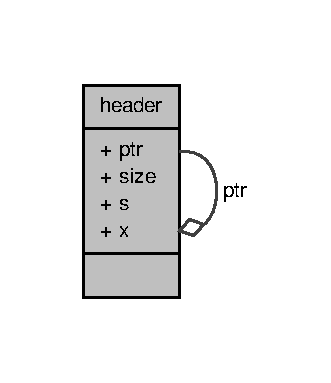
\includegraphics[width=159pt]{unionheader__coll__graph}
\end{center}
\end{figure}
\subsection*{\-Data \-Fields}
\begin{DoxyCompactItemize}
\item 
\begin{tabbing}
xx\=xx\=xx\=xx\=xx\=xx\=xx\=xx\=xx\=\kill
struct \{\\
\>union \hyperlink{unionheader}{header} $\ast$ \hyperlink{unionheader_a0e84d7fb56aa45d0a3eb7083a5ff1b63}{ptr}\\
\>unsigned int \hyperlink{unionheader_aac913b3a1f6ef005d66bf7a84428773e}{size}\\
\} \hyperlink{unionheader_a958d7cb7719f42c07c1a600553d0db44}{s}\\

\end{tabbing}\item 
\hyperlink{mm_8c_aa508dd61e627680e57643837d292d89f}{\-Align} \hyperlink{unionheader_a5f369a9edd645986a45d0c159773c740}{x}
\end{DoxyCompactItemize}


\subsection{\-Detailed \-Description}


\-Definition at line 119 of file mm.\-c.



\subsection{\-Field \-Documentation}
\hypertarget{unionheader_a0e84d7fb56aa45d0a3eb7083a5ff1b63}{\index{header@{header}!ptr@{ptr}}
\index{ptr@{ptr}!header@{header}}
\subsubsection[{ptr}]{\setlength{\rightskip}{0pt plus 5cm}union {\bf header}$\ast$ {\bf ptr}}}\label{unionheader_a0e84d7fb56aa45d0a3eb7083a5ff1b63}


\-Definition at line 121 of file mm.\-c.

\hypertarget{unionheader_a958d7cb7719f42c07c1a600553d0db44}{\index{header@{header}!s@{s}}
\index{s@{s}!header@{header}}
\subsubsection[{s}]{\setlength{\rightskip}{0pt plus 5cm}struct \{ ... \}   {\bf s}}}\label{unionheader_a958d7cb7719f42c07c1a600553d0db44}
\hypertarget{unionheader_aac913b3a1f6ef005d66bf7a84428773e}{\index{header@{header}!size@{size}}
\index{size@{size}!header@{header}}
\subsubsection[{size}]{\setlength{\rightskip}{0pt plus 5cm}unsigned int {\bf size}}}\label{unionheader_aac913b3a1f6ef005d66bf7a84428773e}


\-Definition at line 122 of file mm.\-c.

\hypertarget{unionheader_a5f369a9edd645986a45d0c159773c740}{\index{header@{header}!x@{x}}
\index{x@{x}!header@{header}}
\subsubsection[{x}]{\setlength{\rightskip}{0pt plus 5cm}{\bf \-Align} {\bf x}}}\label{unionheader_a5f369a9edd645986a45d0c159773c740}


\-Definition at line 125 of file mm.\-c.



\-The documentation for this union was generated from the following file\-:\begin{DoxyCompactItemize}
\item 
\hyperlink{mm_8c}{mm.\-c}\end{DoxyCompactItemize}

\hypertarget{structhyp__guest__context}{\section{hyp\-\_\-guest\-\_\-context \-Struct \-Reference}
\label{structhyp__guest__context}\index{hyp\-\_\-guest\-\_\-context@{hyp\-\_\-guest\-\_\-context}}
}


{\ttfamily \#include $<$context.\-h$>$}



\-Collaboration diagram for hyp\-\_\-guest\-\_\-context\-:
\nopagebreak
\begin{figure}[H]
\begin{center}
\leavevmode
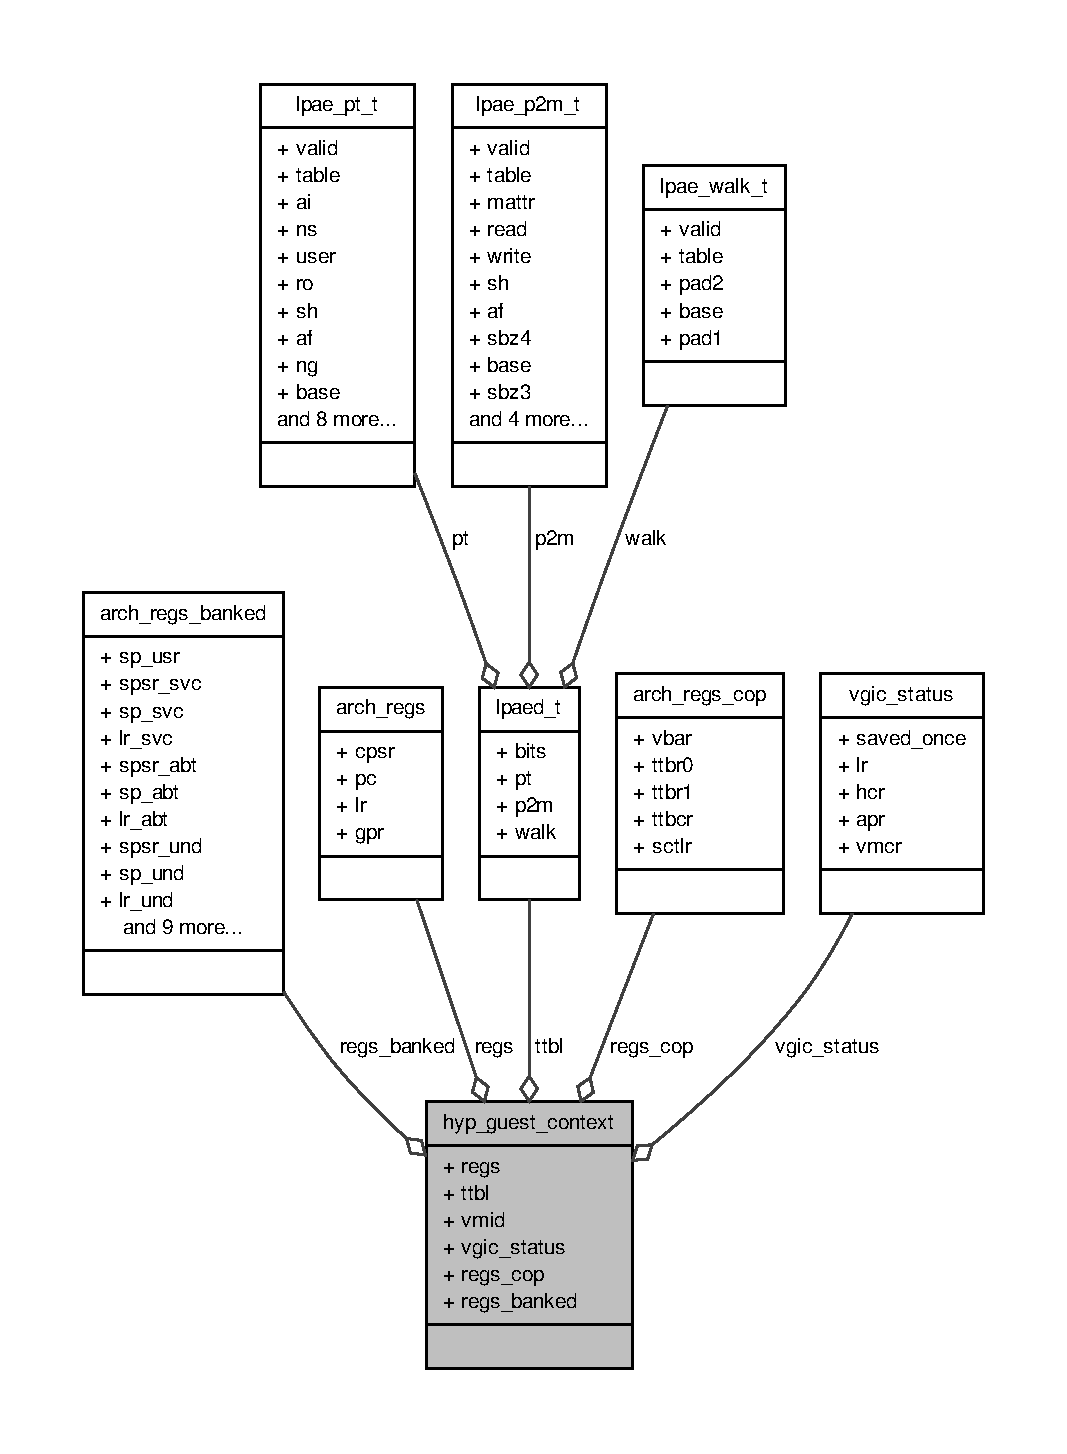
\includegraphics[width=350pt]{structhyp__guest__context__coll__graph}
\end{center}
\end{figure}
\subsection*{\-Data \-Fields}
\begin{DoxyCompactItemize}
\item 
struct \hyperlink{structarch__regs}{arch\-\_\-regs} \hyperlink{structhyp__guest__context_a6fd37717ff9cb8421e3e19acc489b565}{regs}
\item 
\hyperlink{unionlpaed__t}{lpaed\-\_\-t} $\ast$ \hyperlink{structhyp__guest__context_af96dd8c0db5b16addac6cbaa292894d1}{ttbl}
\item 
\hyperlink{hvmm__types_8h_af7e9bd0adfb7d10e7a7a0ee60a5f962c}{vmid\-\_\-t} \hyperlink{structhyp__guest__context_a5aaea0584ec137718b51152ba747628b}{vmid}
\item 
struct \hyperlink{structvgic__status}{vgic\-\_\-status} \hyperlink{structhyp__guest__context_aaf1e3e694ca7bf2cbda2d9817f3e9389}{vgic\-\_\-status}
\item 
struct \hyperlink{structarch__regs__cop}{arch\-\_\-regs\-\_\-cop} \hyperlink{structhyp__guest__context_a216fdbbf2a31b2bef63e2c013f25ce51}{regs\-\_\-cop}
\item 
struct \hyperlink{structarch__regs__banked}{arch\-\_\-regs\-\_\-banked} \hyperlink{structhyp__guest__context_a16825e70a665e6368fce044d9f1fdb07}{regs\-\_\-banked}
\end{DoxyCompactItemize}


\subsection{\-Detailed \-Description}


\-Definition at line 59 of file context.\-h.



\subsection{\-Field \-Documentation}
\hypertarget{structhyp__guest__context_a6fd37717ff9cb8421e3e19acc489b565}{\index{hyp\-\_\-guest\-\_\-context@{hyp\-\_\-guest\-\_\-context}!regs@{regs}}
\index{regs@{regs}!hyp_guest_context@{hyp\-\_\-guest\-\_\-context}}
\subsubsection[{regs}]{\setlength{\rightskip}{0pt plus 5cm}struct {\bf arch\-\_\-regs} {\bf regs}}}\label{structhyp__guest__context_a6fd37717ff9cb8421e3e19acc489b565}


\-Definition at line 60 of file context.\-h.

\hypertarget{structhyp__guest__context_a16825e70a665e6368fce044d9f1fdb07}{\index{hyp\-\_\-guest\-\_\-context@{hyp\-\_\-guest\-\_\-context}!regs\-\_\-banked@{regs\-\_\-banked}}
\index{regs\-\_\-banked@{regs\-\_\-banked}!hyp_guest_context@{hyp\-\_\-guest\-\_\-context}}
\subsubsection[{regs\-\_\-banked}]{\setlength{\rightskip}{0pt plus 5cm}struct {\bf arch\-\_\-regs\-\_\-banked} {\bf regs\-\_\-banked}}}\label{structhyp__guest__context_a16825e70a665e6368fce044d9f1fdb07}


\-Definition at line 65 of file context.\-h.

\hypertarget{structhyp__guest__context_a216fdbbf2a31b2bef63e2c013f25ce51}{\index{hyp\-\_\-guest\-\_\-context@{hyp\-\_\-guest\-\_\-context}!regs\-\_\-cop@{regs\-\_\-cop}}
\index{regs\-\_\-cop@{regs\-\_\-cop}!hyp_guest_context@{hyp\-\_\-guest\-\_\-context}}
\subsubsection[{regs\-\_\-cop}]{\setlength{\rightskip}{0pt plus 5cm}struct {\bf arch\-\_\-regs\-\_\-cop} {\bf regs\-\_\-cop}}}\label{structhyp__guest__context_a216fdbbf2a31b2bef63e2c013f25ce51}


\-Definition at line 64 of file context.\-h.

\hypertarget{structhyp__guest__context_af96dd8c0db5b16addac6cbaa292894d1}{\index{hyp\-\_\-guest\-\_\-context@{hyp\-\_\-guest\-\_\-context}!ttbl@{ttbl}}
\index{ttbl@{ttbl}!hyp_guest_context@{hyp\-\_\-guest\-\_\-context}}
\subsubsection[{ttbl}]{\setlength{\rightskip}{0pt plus 5cm}{\bf lpaed\-\_\-t}$\ast$ {\bf ttbl}}}\label{structhyp__guest__context_af96dd8c0db5b16addac6cbaa292894d1}


\-Definition at line 61 of file context.\-h.

\hypertarget{structhyp__guest__context_aaf1e3e694ca7bf2cbda2d9817f3e9389}{\index{hyp\-\_\-guest\-\_\-context@{hyp\-\_\-guest\-\_\-context}!vgic\-\_\-status@{vgic\-\_\-status}}
\index{vgic\-\_\-status@{vgic\-\_\-status}!hyp_guest_context@{hyp\-\_\-guest\-\_\-context}}
\subsubsection[{vgic\-\_\-status}]{\setlength{\rightskip}{0pt plus 5cm}struct {\bf vgic\-\_\-status} {\bf vgic\-\_\-status}}}\label{structhyp__guest__context_aaf1e3e694ca7bf2cbda2d9817f3e9389}


\-Definition at line 63 of file context.\-h.

\hypertarget{structhyp__guest__context_a5aaea0584ec137718b51152ba747628b}{\index{hyp\-\_\-guest\-\_\-context@{hyp\-\_\-guest\-\_\-context}!vmid@{vmid}}
\index{vmid@{vmid}!hyp_guest_context@{hyp\-\_\-guest\-\_\-context}}
\subsubsection[{vmid}]{\setlength{\rightskip}{0pt plus 5cm}{\bf vmid\-\_\-t} {\bf vmid}}}\label{structhyp__guest__context_a5aaea0584ec137718b51152ba747628b}


\-Definition at line 62 of file context.\-h.



\-The documentation for this struct was generated from the following file\-:\begin{DoxyCompactItemize}
\item 
\hyperlink{context_8h}{context.\-h}\end{DoxyCompactItemize}

\hypertarget{structlpae__p2m__t}{\section{lpae\-\_\-p2m\-\_\-t \-Struct \-Reference}
\label{structlpae__p2m__t}\index{lpae\-\_\-p2m\-\_\-t@{lpae\-\_\-p2m\-\_\-t}}
}


{\ttfamily \#include $<$lpae.\-h$>$}

\subsection*{\-Data \-Fields}
\begin{DoxyCompactItemize}
\item 
unsigned long \hyperlink{structlpae__p2m__t_a7bcbc21e402fb9e3dc07789d414ef17c}{valid}\-:1
\item 
unsigned long \hyperlink{structlpae__p2m__t_afe6d8cf4d4c78126d82831e6d5ef5483}{table}\-:1
\item 
unsigned long \hyperlink{structlpae__p2m__t_abb75a9f607e52a07db6a528672e0ccd6}{mattr}\-:4
\item 
unsigned long \hyperlink{structlpae__p2m__t_a414a71904272e5b5fce01917028fb426}{read}\-:1
\item 
unsigned long \hyperlink{structlpae__p2m__t_aff1f8e39a81cacd30783afe206b0835e}{write}\-:1
\item 
unsigned long \hyperlink{structlpae__p2m__t_a8388cd14eb45903279fca66cedfa5ec7}{sh}\-:2
\item 
unsigned long \hyperlink{structlpae__p2m__t_a0f5634df96396057ace3b5f21b1cb381}{af}\-:1
\item 
unsigned long \hyperlink{structlpae__p2m__t_a38ba2ebd33232186b46dd6c586cdef25}{sbz4}\-:1
\item 
unsigned long \hyperlink{structlpae__p2m__t_a74f95eab64fb23344e30879684489f6f}{base}\-:28
\item 
unsigned long \hyperlink{structlpae__p2m__t_abec53fb8579fdb4fbbed7e95ca3433d1}{sbz3}\-:12
\item 
unsigned long \hyperlink{structlpae__p2m__t_a6b9526601b3748535699c90ec4d83a70}{hint}\-:1
\item 
unsigned long \hyperlink{structlpae__p2m__t_af8da50342df58644c092236709963e4c}{sbz2}\-:1
\item 
unsigned long \hyperlink{structlpae__p2m__t_a14c376b2856f5d0a79874df679a35d94}{xn}\-:1
\item 
unsigned long \hyperlink{structlpae__p2m__t_a09631255ee08cc058acd8bc1caff188c}{avail}\-:4
\item 
unsigned long \hyperlink{structlpae__p2m__t_aaaf6b94202af054e3777a0fc8938ea85}{sbz1}\-:5
\end{DoxyCompactItemize}


\subsection{\-Detailed \-Description}


\-Definition at line 78 of file lpae.\-h.



\subsection{\-Field \-Documentation}
\hypertarget{structlpae__p2m__t_a0f5634df96396057ace3b5f21b1cb381}{\index{lpae\-\_\-p2m\-\_\-t@{lpae\-\_\-p2m\-\_\-t}!af@{af}}
\index{af@{af}!lpae_p2m_t@{lpae\-\_\-p2m\-\_\-t}}
\subsubsection[{af}]{\setlength{\rightskip}{0pt plus 5cm}unsigned long {\bf af}}}\label{structlpae__p2m__t_a0f5634df96396057ace3b5f21b1cb381}


\-Definition at line 89 of file lpae.\-h.

\hypertarget{structlpae__p2m__t_a09631255ee08cc058acd8bc1caff188c}{\index{lpae\-\_\-p2m\-\_\-t@{lpae\-\_\-p2m\-\_\-t}!avail@{avail}}
\index{avail@{avail}!lpae_p2m_t@{lpae\-\_\-p2m\-\_\-t}}
\subsubsection[{avail}]{\setlength{\rightskip}{0pt plus 5cm}unsigned long {\bf avail}}}\label{structlpae__p2m__t_a09631255ee08cc058acd8bc1caff188c}


\-Definition at line 101 of file lpae.\-h.

\hypertarget{structlpae__p2m__t_a74f95eab64fb23344e30879684489f6f}{\index{lpae\-\_\-p2m\-\_\-t@{lpae\-\_\-p2m\-\_\-t}!base@{base}}
\index{base@{base}!lpae_p2m_t@{lpae\-\_\-p2m\-\_\-t}}
\subsubsection[{base}]{\setlength{\rightskip}{0pt plus 5cm}unsigned long {\bf base}}}\label{structlpae__p2m__t_a74f95eab64fb23344e30879684489f6f}


\-Definition at line 93 of file lpae.\-h.

\hypertarget{structlpae__p2m__t_a6b9526601b3748535699c90ec4d83a70}{\index{lpae\-\_\-p2m\-\_\-t@{lpae\-\_\-p2m\-\_\-t}!hint@{hint}}
\index{hint@{hint}!lpae_p2m_t@{lpae\-\_\-p2m\-\_\-t}}
\subsubsection[{hint}]{\setlength{\rightskip}{0pt plus 5cm}unsigned long {\bf hint}}}\label{structlpae__p2m__t_a6b9526601b3748535699c90ec4d83a70}


\-Definition at line 98 of file lpae.\-h.

\hypertarget{structlpae__p2m__t_abb75a9f607e52a07db6a528672e0ccd6}{\index{lpae\-\_\-p2m\-\_\-t@{lpae\-\_\-p2m\-\_\-t}!mattr@{mattr}}
\index{mattr@{mattr}!lpae_p2m_t@{lpae\-\_\-p2m\-\_\-t}}
\subsubsection[{mattr}]{\setlength{\rightskip}{0pt plus 5cm}unsigned long {\bf mattr}}}\label{structlpae__p2m__t_abb75a9f607e52a07db6a528672e0ccd6}


\-Definition at line 85 of file lpae.\-h.

\hypertarget{structlpae__p2m__t_a414a71904272e5b5fce01917028fb426}{\index{lpae\-\_\-p2m\-\_\-t@{lpae\-\_\-p2m\-\_\-t}!read@{read}}
\index{read@{read}!lpae_p2m_t@{lpae\-\_\-p2m\-\_\-t}}
\subsubsection[{read}]{\setlength{\rightskip}{0pt plus 5cm}unsigned long {\bf read}}}\label{structlpae__p2m__t_a414a71904272e5b5fce01917028fb426}


\-Definition at line 86 of file lpae.\-h.

\hypertarget{structlpae__p2m__t_aaaf6b94202af054e3777a0fc8938ea85}{\index{lpae\-\_\-p2m\-\_\-t@{lpae\-\_\-p2m\-\_\-t}!sbz1@{sbz1}}
\index{sbz1@{sbz1}!lpae_p2m_t@{lpae\-\_\-p2m\-\_\-t}}
\subsubsection[{sbz1}]{\setlength{\rightskip}{0pt plus 5cm}unsigned long {\bf sbz1}}}\label{structlpae__p2m__t_aaaf6b94202af054e3777a0fc8938ea85}


\-Definition at line 103 of file lpae.\-h.

\hypertarget{structlpae__p2m__t_af8da50342df58644c092236709963e4c}{\index{lpae\-\_\-p2m\-\_\-t@{lpae\-\_\-p2m\-\_\-t}!sbz2@{sbz2}}
\index{sbz2@{sbz2}!lpae_p2m_t@{lpae\-\_\-p2m\-\_\-t}}
\subsubsection[{sbz2}]{\setlength{\rightskip}{0pt plus 5cm}unsigned long {\bf sbz2}}}\label{structlpae__p2m__t_af8da50342df58644c092236709963e4c}


\-Definition at line 99 of file lpae.\-h.

\hypertarget{structlpae__p2m__t_abec53fb8579fdb4fbbed7e95ca3433d1}{\index{lpae\-\_\-p2m\-\_\-t@{lpae\-\_\-p2m\-\_\-t}!sbz3@{sbz3}}
\index{sbz3@{sbz3}!lpae_p2m_t@{lpae\-\_\-p2m\-\_\-t}}
\subsubsection[{sbz3}]{\setlength{\rightskip}{0pt plus 5cm}unsigned long {\bf sbz3}}}\label{structlpae__p2m__t_abec53fb8579fdb4fbbed7e95ca3433d1}


\-Definition at line 94 of file lpae.\-h.

\hypertarget{structlpae__p2m__t_a38ba2ebd33232186b46dd6c586cdef25}{\index{lpae\-\_\-p2m\-\_\-t@{lpae\-\_\-p2m\-\_\-t}!sbz4@{sbz4}}
\index{sbz4@{sbz4}!lpae_p2m_t@{lpae\-\_\-p2m\-\_\-t}}
\subsubsection[{sbz4}]{\setlength{\rightskip}{0pt plus 5cm}unsigned long {\bf sbz4}}}\label{structlpae__p2m__t_a38ba2ebd33232186b46dd6c586cdef25}


\-Definition at line 90 of file lpae.\-h.

\hypertarget{structlpae__p2m__t_a8388cd14eb45903279fca66cedfa5ec7}{\index{lpae\-\_\-p2m\-\_\-t@{lpae\-\_\-p2m\-\_\-t}!sh@{sh}}
\index{sh@{sh}!lpae_p2m_t@{lpae\-\_\-p2m\-\_\-t}}
\subsubsection[{sh}]{\setlength{\rightskip}{0pt plus 5cm}unsigned long {\bf sh}}}\label{structlpae__p2m__t_a8388cd14eb45903279fca66cedfa5ec7}


\-Definition at line 88 of file lpae.\-h.

\hypertarget{structlpae__p2m__t_afe6d8cf4d4c78126d82831e6d5ef5483}{\index{lpae\-\_\-p2m\-\_\-t@{lpae\-\_\-p2m\-\_\-t}!table@{table}}
\index{table@{table}!lpae_p2m_t@{lpae\-\_\-p2m\-\_\-t}}
\subsubsection[{table}]{\setlength{\rightskip}{0pt plus 5cm}unsigned long {\bf table}}}\label{structlpae__p2m__t_afe6d8cf4d4c78126d82831e6d5ef5483}


\-Definition at line 81 of file lpae.\-h.

\hypertarget{structlpae__p2m__t_a7bcbc21e402fb9e3dc07789d414ef17c}{\index{lpae\-\_\-p2m\-\_\-t@{lpae\-\_\-p2m\-\_\-t}!valid@{valid}}
\index{valid@{valid}!lpae_p2m_t@{lpae\-\_\-p2m\-\_\-t}}
\subsubsection[{valid}]{\setlength{\rightskip}{0pt plus 5cm}unsigned long {\bf valid}}}\label{structlpae__p2m__t_a7bcbc21e402fb9e3dc07789d414ef17c}


\-Definition at line 80 of file lpae.\-h.

\hypertarget{structlpae__p2m__t_aff1f8e39a81cacd30783afe206b0835e}{\index{lpae\-\_\-p2m\-\_\-t@{lpae\-\_\-p2m\-\_\-t}!write@{write}}
\index{write@{write}!lpae_p2m_t@{lpae\-\_\-p2m\-\_\-t}}
\subsubsection[{write}]{\setlength{\rightskip}{0pt plus 5cm}unsigned long {\bf write}}}\label{structlpae__p2m__t_aff1f8e39a81cacd30783afe206b0835e}


\-Definition at line 87 of file lpae.\-h.

\hypertarget{structlpae__p2m__t_a14c376b2856f5d0a79874df679a35d94}{\index{lpae\-\_\-p2m\-\_\-t@{lpae\-\_\-p2m\-\_\-t}!xn@{xn}}
\index{xn@{xn}!lpae_p2m_t@{lpae\-\_\-p2m\-\_\-t}}
\subsubsection[{xn}]{\setlength{\rightskip}{0pt plus 5cm}unsigned long {\bf xn}}}\label{structlpae__p2m__t_a14c376b2856f5d0a79874df679a35d94}


\-Definition at line 100 of file lpae.\-h.



\-The documentation for this struct was generated from the following file\-:\begin{DoxyCompactItemize}
\item 
\hyperlink{lpae_8h}{lpae.\-h}\end{DoxyCompactItemize}

\hypertarget{structlpae__pt__t}{\section{lpae\-\_\-pt\-\_\-t \-Struct \-Reference}
\label{structlpae__pt__t}\index{lpae\-\_\-pt\-\_\-t@{lpae\-\_\-pt\-\_\-t}}
}


{\ttfamily \#include $<$lpae.\-h$>$}

\subsection*{\-Data \-Fields}
\begin{DoxyCompactItemize}
\item 
unsigned long \hyperlink{structlpae__pt__t_a7bcbc21e402fb9e3dc07789d414ef17c}{valid}\-:1
\item 
unsigned long \hyperlink{structlpae__pt__t_afe6d8cf4d4c78126d82831e6d5ef5483}{table}\-:1
\item 
unsigned long \hyperlink{structlpae__pt__t_ab49c18e57563921295ef8942744109e9}{ai}\-:3
\item 
unsigned long \hyperlink{structlpae__pt__t_a0c9a7685114f88cfb4cc879031ccd9c2}{ns}\-:1
\item 
unsigned long \hyperlink{structlpae__pt__t_a410008f6ab71b4ad6f00e5a0aa591f8a}{user}\-:1
\item 
unsigned long \hyperlink{structlpae__pt__t_aab6cd914c5bb4ca31f78a11024e97a05}{ro}\-:1
\item 
unsigned long \hyperlink{structlpae__pt__t_a8388cd14eb45903279fca66cedfa5ec7}{sh}\-:2
\item 
unsigned long \hyperlink{structlpae__pt__t_a0f5634df96396057ace3b5f21b1cb381}{af}\-:1
\item 
unsigned long \hyperlink{structlpae__pt__t_a7e9b55fee8cbf4a7f95905d93b8eb8f6}{ng}\-:1
\item 
unsigned long \hyperlink{structlpae__pt__t_a74f95eab64fb23344e30879684489f6f}{base}\-:28
\item 
unsigned long \hyperlink{structlpae__pt__t_ae5b1c215d1172ca33cb4cc70b4484406}{sbz}\-:12
\item 
unsigned long \hyperlink{structlpae__pt__t_a6b9526601b3748535699c90ec4d83a70}{hint}\-:1
\item 
unsigned long \hyperlink{structlpae__pt__t_ac47dd62f5bdb2c1f62fe7a83f23b8902}{pxn}\-:1
\item 
unsigned long \hyperlink{structlpae__pt__t_a14c376b2856f5d0a79874df679a35d94}{xn}\-:1
\item 
unsigned long \hyperlink{structlpae__pt__t_a09631255ee08cc058acd8bc1caff188c}{avail}\-:4
\item 
unsigned long \hyperlink{structlpae__pt__t_a23cf82105349863d2f84c49d7410180a}{pxnt}\-:1
\item 
unsigned long \hyperlink{structlpae__pt__t_a8fc352a6df3247a0039ad7dccaf666d8}{xnt}\-:1
\item 
unsigned long \hyperlink{structlpae__pt__t_a27acf8b422b08ad2eee782c2cd01f1df}{apt}\-:2
\item 
unsigned long \hyperlink{structlpae__pt__t_adb22eee76377f57c572e33df1a66a27a}{nst}\-:1
\end{DoxyCompactItemize}


\subsection{\-Detailed \-Description}


\-Definition at line 42 of file lpae.\-h.



\subsection{\-Field \-Documentation}
\hypertarget{structlpae__pt__t_a0f5634df96396057ace3b5f21b1cb381}{\index{lpae\-\_\-pt\-\_\-t@{lpae\-\_\-pt\-\_\-t}!af@{af}}
\index{af@{af}!lpae_pt_t@{lpae\-\_\-pt\-\_\-t}}
\subsubsection[{af}]{\setlength{\rightskip}{0pt plus 5cm}unsigned long {\bf af}}}\label{structlpae__pt__t_a0f5634df96396057ace3b5f21b1cb381}


\-Definition at line 54 of file lpae.\-h.

\hypertarget{structlpae__pt__t_ab49c18e57563921295ef8942744109e9}{\index{lpae\-\_\-pt\-\_\-t@{lpae\-\_\-pt\-\_\-t}!ai@{ai}}
\index{ai@{ai}!lpae_pt_t@{lpae\-\_\-pt\-\_\-t}}
\subsubsection[{ai}]{\setlength{\rightskip}{0pt plus 5cm}unsigned long {\bf ai}}}\label{structlpae__pt__t_ab49c18e57563921295ef8942744109e9}


\-Definition at line 49 of file lpae.\-h.

\hypertarget{structlpae__pt__t_a27acf8b422b08ad2eee782c2cd01f1df}{\index{lpae\-\_\-pt\-\_\-t@{lpae\-\_\-pt\-\_\-t}!apt@{apt}}
\index{apt@{apt}!lpae_pt_t@{lpae\-\_\-pt\-\_\-t}}
\subsubsection[{apt}]{\setlength{\rightskip}{0pt plus 5cm}unsigned long {\bf apt}}}\label{structlpae__pt__t_a27acf8b422b08ad2eee782c2cd01f1df}


\-Definition at line 72 of file lpae.\-h.

\hypertarget{structlpae__pt__t_a09631255ee08cc058acd8bc1caff188c}{\index{lpae\-\_\-pt\-\_\-t@{lpae\-\_\-pt\-\_\-t}!avail@{avail}}
\index{avail@{avail}!lpae_pt_t@{lpae\-\_\-pt\-\_\-t}}
\subsubsection[{avail}]{\setlength{\rightskip}{0pt plus 5cm}unsigned long {\bf avail}}}\label{structlpae__pt__t_a09631255ee08cc058acd8bc1caff188c}


\-Definition at line 66 of file lpae.\-h.

\hypertarget{structlpae__pt__t_a74f95eab64fb23344e30879684489f6f}{\index{lpae\-\_\-pt\-\_\-t@{lpae\-\_\-pt\-\_\-t}!base@{base}}
\index{base@{base}!lpae_pt_t@{lpae\-\_\-pt\-\_\-t}}
\subsubsection[{base}]{\setlength{\rightskip}{0pt plus 5cm}unsigned long {\bf base}}}\label{structlpae__pt__t_a74f95eab64fb23344e30879684489f6f}


\-Definition at line 58 of file lpae.\-h.

\hypertarget{structlpae__pt__t_a6b9526601b3748535699c90ec4d83a70}{\index{lpae\-\_\-pt\-\_\-t@{lpae\-\_\-pt\-\_\-t}!hint@{hint}}
\index{hint@{hint}!lpae_pt_t@{lpae\-\_\-pt\-\_\-t}}
\subsubsection[{hint}]{\setlength{\rightskip}{0pt plus 5cm}unsigned long {\bf hint}}}\label{structlpae__pt__t_a6b9526601b3748535699c90ec4d83a70}


\-Definition at line 63 of file lpae.\-h.

\hypertarget{structlpae__pt__t_a7e9b55fee8cbf4a7f95905d93b8eb8f6}{\index{lpae\-\_\-pt\-\_\-t@{lpae\-\_\-pt\-\_\-t}!ng@{ng}}
\index{ng@{ng}!lpae_pt_t@{lpae\-\_\-pt\-\_\-t}}
\subsubsection[{ng}]{\setlength{\rightskip}{0pt plus 5cm}unsigned long {\bf ng}}}\label{structlpae__pt__t_a7e9b55fee8cbf4a7f95905d93b8eb8f6}


\-Definition at line 55 of file lpae.\-h.

\hypertarget{structlpae__pt__t_a0c9a7685114f88cfb4cc879031ccd9c2}{\index{lpae\-\_\-pt\-\_\-t@{lpae\-\_\-pt\-\_\-t}!ns@{ns}}
\index{ns@{ns}!lpae_pt_t@{lpae\-\_\-pt\-\_\-t}}
\subsubsection[{ns}]{\setlength{\rightskip}{0pt plus 5cm}unsigned long {\bf ns}}}\label{structlpae__pt__t_a0c9a7685114f88cfb4cc879031ccd9c2}


\-Definition at line 50 of file lpae.\-h.

\hypertarget{structlpae__pt__t_adb22eee76377f57c572e33df1a66a27a}{\index{lpae\-\_\-pt\-\_\-t@{lpae\-\_\-pt\-\_\-t}!nst@{nst}}
\index{nst@{nst}!lpae_pt_t@{lpae\-\_\-pt\-\_\-t}}
\subsubsection[{nst}]{\setlength{\rightskip}{0pt plus 5cm}unsigned long {\bf nst}}}\label{structlpae__pt__t_adb22eee76377f57c572e33df1a66a27a}


\-Definition at line 73 of file lpae.\-h.

\hypertarget{structlpae__pt__t_ac47dd62f5bdb2c1f62fe7a83f23b8902}{\index{lpae\-\_\-pt\-\_\-t@{lpae\-\_\-pt\-\_\-t}!pxn@{pxn}}
\index{pxn@{pxn}!lpae_pt_t@{lpae\-\_\-pt\-\_\-t}}
\subsubsection[{pxn}]{\setlength{\rightskip}{0pt plus 5cm}unsigned long {\bf pxn}}}\label{structlpae__pt__t_ac47dd62f5bdb2c1f62fe7a83f23b8902}


\-Definition at line 64 of file lpae.\-h.

\hypertarget{structlpae__pt__t_a23cf82105349863d2f84c49d7410180a}{\index{lpae\-\_\-pt\-\_\-t@{lpae\-\_\-pt\-\_\-t}!pxnt@{pxnt}}
\index{pxnt@{pxnt}!lpae_pt_t@{lpae\-\_\-pt\-\_\-t}}
\subsubsection[{pxnt}]{\setlength{\rightskip}{0pt plus 5cm}unsigned long {\bf pxnt}}}\label{structlpae__pt__t_a23cf82105349863d2f84c49d7410180a}


\-Definition at line 70 of file lpae.\-h.

\hypertarget{structlpae__pt__t_aab6cd914c5bb4ca31f78a11024e97a05}{\index{lpae\-\_\-pt\-\_\-t@{lpae\-\_\-pt\-\_\-t}!ro@{ro}}
\index{ro@{ro}!lpae_pt_t@{lpae\-\_\-pt\-\_\-t}}
\subsubsection[{ro}]{\setlength{\rightskip}{0pt plus 5cm}unsigned long {\bf ro}}}\label{structlpae__pt__t_aab6cd914c5bb4ca31f78a11024e97a05}


\-Definition at line 52 of file lpae.\-h.

\hypertarget{structlpae__pt__t_ae5b1c215d1172ca33cb4cc70b4484406}{\index{lpae\-\_\-pt\-\_\-t@{lpae\-\_\-pt\-\_\-t}!sbz@{sbz}}
\index{sbz@{sbz}!lpae_pt_t@{lpae\-\_\-pt\-\_\-t}}
\subsubsection[{sbz}]{\setlength{\rightskip}{0pt plus 5cm}unsigned long {\bf sbz}}}\label{structlpae__pt__t_ae5b1c215d1172ca33cb4cc70b4484406}


\-Definition at line 59 of file lpae.\-h.

\hypertarget{structlpae__pt__t_a8388cd14eb45903279fca66cedfa5ec7}{\index{lpae\-\_\-pt\-\_\-t@{lpae\-\_\-pt\-\_\-t}!sh@{sh}}
\index{sh@{sh}!lpae_pt_t@{lpae\-\_\-pt\-\_\-t}}
\subsubsection[{sh}]{\setlength{\rightskip}{0pt plus 5cm}unsigned long {\bf sh}}}\label{structlpae__pt__t_a8388cd14eb45903279fca66cedfa5ec7}


\-Definition at line 53 of file lpae.\-h.

\hypertarget{structlpae__pt__t_afe6d8cf4d4c78126d82831e6d5ef5483}{\index{lpae\-\_\-pt\-\_\-t@{lpae\-\_\-pt\-\_\-t}!table@{table}}
\index{table@{table}!lpae_pt_t@{lpae\-\_\-pt\-\_\-t}}
\subsubsection[{table}]{\setlength{\rightskip}{0pt plus 5cm}unsigned long {\bf table}}}\label{structlpae__pt__t_afe6d8cf4d4c78126d82831e6d5ef5483}


\-Definition at line 45 of file lpae.\-h.

\hypertarget{structlpae__pt__t_a410008f6ab71b4ad6f00e5a0aa591f8a}{\index{lpae\-\_\-pt\-\_\-t@{lpae\-\_\-pt\-\_\-t}!user@{user}}
\index{user@{user}!lpae_pt_t@{lpae\-\_\-pt\-\_\-t}}
\subsubsection[{user}]{\setlength{\rightskip}{0pt plus 5cm}unsigned long {\bf user}}}\label{structlpae__pt__t_a410008f6ab71b4ad6f00e5a0aa591f8a}


\-Definition at line 51 of file lpae.\-h.

\hypertarget{structlpae__pt__t_a7bcbc21e402fb9e3dc07789d414ef17c}{\index{lpae\-\_\-pt\-\_\-t@{lpae\-\_\-pt\-\_\-t}!valid@{valid}}
\index{valid@{valid}!lpae_pt_t@{lpae\-\_\-pt\-\_\-t}}
\subsubsection[{valid}]{\setlength{\rightskip}{0pt plus 5cm}unsigned long {\bf valid}}}\label{structlpae__pt__t_a7bcbc21e402fb9e3dc07789d414ef17c}


\-Definition at line 44 of file lpae.\-h.

\hypertarget{structlpae__pt__t_a14c376b2856f5d0a79874df679a35d94}{\index{lpae\-\_\-pt\-\_\-t@{lpae\-\_\-pt\-\_\-t}!xn@{xn}}
\index{xn@{xn}!lpae_pt_t@{lpae\-\_\-pt\-\_\-t}}
\subsubsection[{xn}]{\setlength{\rightskip}{0pt plus 5cm}unsigned long {\bf xn}}}\label{structlpae__pt__t_a14c376b2856f5d0a79874df679a35d94}


\-Definition at line 65 of file lpae.\-h.

\hypertarget{structlpae__pt__t_a8fc352a6df3247a0039ad7dccaf666d8}{\index{lpae\-\_\-pt\-\_\-t@{lpae\-\_\-pt\-\_\-t}!xnt@{xnt}}
\index{xnt@{xnt}!lpae_pt_t@{lpae\-\_\-pt\-\_\-t}}
\subsubsection[{xnt}]{\setlength{\rightskip}{0pt plus 5cm}unsigned long {\bf xnt}}}\label{structlpae__pt__t_a8fc352a6df3247a0039ad7dccaf666d8}


\-Definition at line 71 of file lpae.\-h.



\-The documentation for this struct was generated from the following file\-:\begin{DoxyCompactItemize}
\item 
\hyperlink{lpae_8h}{lpae.\-h}\end{DoxyCompactItemize}

\hypertarget{structlpae__walk__t}{\section{lpae\-\_\-walk\-\_\-t \-Struct \-Reference}
\label{structlpae__walk__t}\index{lpae\-\_\-walk\-\_\-t@{lpae\-\_\-walk\-\_\-t}}
}


{\ttfamily \#include $<$lpae.\-h$>$}

\subsection*{\-Data \-Fields}
\begin{DoxyCompactItemize}
\item 
unsigned long \hyperlink{structlpae__walk__t_a7bcbc21e402fb9e3dc07789d414ef17c}{valid}\-:1
\item 
unsigned long \hyperlink{structlpae__walk__t_afe6d8cf4d4c78126d82831e6d5ef5483}{table}\-:1
\item 
unsigned long \hyperlink{structlpae__walk__t_a3c41899b360fc210cecdadafb8496709}{pad2}\-:10
\item 
unsigned long \hyperlink{structlpae__walk__t_a74f95eab64fb23344e30879684489f6f}{base}\-:28
\item 
unsigned long \hyperlink{structlpae__walk__t_abd440cbf12babccd9a6b85615adb551d}{pad1}\-:24
\end{DoxyCompactItemize}


\subsection{\-Detailed \-Description}


\-Definition at line 111 of file lpae.\-h.



\subsection{\-Field \-Documentation}
\hypertarget{structlpae__walk__t_a74f95eab64fb23344e30879684489f6f}{\index{lpae\-\_\-walk\-\_\-t@{lpae\-\_\-walk\-\_\-t}!base@{base}}
\index{base@{base}!lpae_walk_t@{lpae\-\_\-walk\-\_\-t}}
\subsubsection[{base}]{\setlength{\rightskip}{0pt plus 5cm}unsigned long {\bf base}}}\label{structlpae__walk__t_a74f95eab64fb23344e30879684489f6f}


\-Definition at line 119 of file lpae.\-h.

\hypertarget{structlpae__walk__t_abd440cbf12babccd9a6b85615adb551d}{\index{lpae\-\_\-walk\-\_\-t@{lpae\-\_\-walk\-\_\-t}!pad1@{pad1}}
\index{pad1@{pad1}!lpae_walk_t@{lpae\-\_\-walk\-\_\-t}}
\subsubsection[{pad1}]{\setlength{\rightskip}{0pt plus 5cm}unsigned long {\bf pad1}}}\label{structlpae__walk__t_abd440cbf12babccd9a6b85615adb551d}


\-Definition at line 121 of file lpae.\-h.

\hypertarget{structlpae__walk__t_a3c41899b360fc210cecdadafb8496709}{\index{lpae\-\_\-walk\-\_\-t@{lpae\-\_\-walk\-\_\-t}!pad2@{pad2}}
\index{pad2@{pad2}!lpae_walk_t@{lpae\-\_\-walk\-\_\-t}}
\subsubsection[{pad2}]{\setlength{\rightskip}{0pt plus 5cm}unsigned long {\bf pad2}}}\label{structlpae__walk__t_a3c41899b360fc210cecdadafb8496709}


\-Definition at line 116 of file lpae.\-h.

\hypertarget{structlpae__walk__t_afe6d8cf4d4c78126d82831e6d5ef5483}{\index{lpae\-\_\-walk\-\_\-t@{lpae\-\_\-walk\-\_\-t}!table@{table}}
\index{table@{table}!lpae_walk_t@{lpae\-\_\-walk\-\_\-t}}
\subsubsection[{table}]{\setlength{\rightskip}{0pt plus 5cm}unsigned long {\bf table}}}\label{structlpae__walk__t_afe6d8cf4d4c78126d82831e6d5ef5483}


\-Definition at line 114 of file lpae.\-h.

\hypertarget{structlpae__walk__t_a7bcbc21e402fb9e3dc07789d414ef17c}{\index{lpae\-\_\-walk\-\_\-t@{lpae\-\_\-walk\-\_\-t}!valid@{valid}}
\index{valid@{valid}!lpae_walk_t@{lpae\-\_\-walk\-\_\-t}}
\subsubsection[{valid}]{\setlength{\rightskip}{0pt plus 5cm}unsigned long {\bf valid}}}\label{structlpae__walk__t_a7bcbc21e402fb9e3dc07789d414ef17c}


\-Definition at line 113 of file lpae.\-h.



\-The documentation for this struct was generated from the following file\-:\begin{DoxyCompactItemize}
\item 
\hyperlink{lpae_8h}{lpae.\-h}\end{DoxyCompactItemize}

\hypertarget{unionlpaed__t}{\section{lpaed\-\_\-t \-Union \-Reference}
\label{unionlpaed__t}\index{lpaed\-\_\-t@{lpaed\-\_\-t}}
}


{\ttfamily \#include $<$lpae.\-h$>$}



\-Collaboration diagram for lpaed\-\_\-t\-:
\nopagebreak
\begin{figure}[H]
\begin{center}
\leavevmode
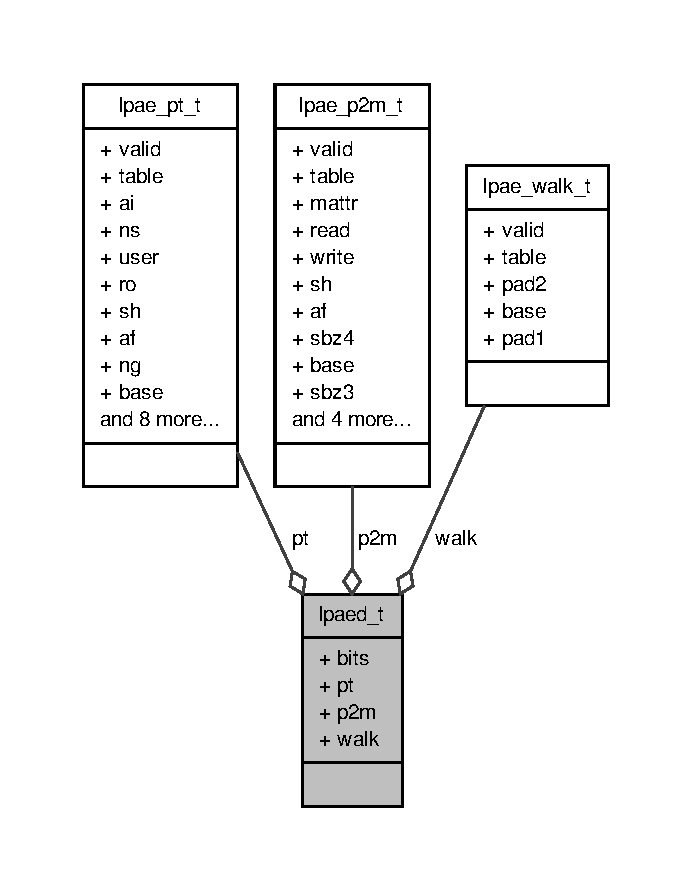
\includegraphics[width=332pt]{unionlpaed__t__coll__graph}
\end{center}
\end{figure}
\subsection*{\-Data \-Fields}
\begin{DoxyCompactItemize}
\item 
\hyperlink{arch__types_8h_aaa5d1cd013383c889537491c3cfd9aad}{uint64\-\_\-t} \hyperlink{unionlpaed__t_a824af546b997aeefcb71a5fe0eda3a0a}{bits}
\item 
\hyperlink{structlpae__pt__t}{lpae\-\_\-pt\-\_\-t} \hyperlink{unionlpaed__t_acddbc2df6cd0023f42d3076bd91794df}{pt}
\item 
\hyperlink{structlpae__p2m__t}{lpae\-\_\-p2m\-\_\-t} \hyperlink{unionlpaed__t_a99761ab7c6ee8d403ed1a7483155089f}{p2m}
\item 
\hyperlink{structlpae__walk__t}{lpae\-\_\-walk\-\_\-t} \hyperlink{unionlpaed__t_a17c7b75f6d0703c70a29b68451c901f2}{walk}
\end{DoxyCompactItemize}


\subsection{\-Detailed \-Description}


\-Definition at line 124 of file lpae.\-h.



\subsection{\-Field \-Documentation}
\hypertarget{unionlpaed__t_a824af546b997aeefcb71a5fe0eda3a0a}{\index{lpaed\-\_\-t@{lpaed\-\_\-t}!bits@{bits}}
\index{bits@{bits}!lpaed_t@{lpaed\-\_\-t}}
\subsubsection[{bits}]{\setlength{\rightskip}{0pt plus 5cm}{\bf uint64\-\_\-t} {\bf bits}}}\label{unionlpaed__t_a824af546b997aeefcb71a5fe0eda3a0a}


\-Definition at line 125 of file lpae.\-h.

\hypertarget{unionlpaed__t_a99761ab7c6ee8d403ed1a7483155089f}{\index{lpaed\-\_\-t@{lpaed\-\_\-t}!p2m@{p2m}}
\index{p2m@{p2m}!lpaed_t@{lpaed\-\_\-t}}
\subsubsection[{p2m}]{\setlength{\rightskip}{0pt plus 5cm}{\bf lpae\-\_\-p2m\-\_\-t} {\bf p2m}}}\label{unionlpaed__t_a99761ab7c6ee8d403ed1a7483155089f}


\-Definition at line 127 of file lpae.\-h.

\hypertarget{unionlpaed__t_acddbc2df6cd0023f42d3076bd91794df}{\index{lpaed\-\_\-t@{lpaed\-\_\-t}!pt@{pt}}
\index{pt@{pt}!lpaed_t@{lpaed\-\_\-t}}
\subsubsection[{pt}]{\setlength{\rightskip}{0pt plus 5cm}{\bf lpae\-\_\-pt\-\_\-t} {\bf pt}}}\label{unionlpaed__t_acddbc2df6cd0023f42d3076bd91794df}


\-Definition at line 126 of file lpae.\-h.

\hypertarget{unionlpaed__t_a17c7b75f6d0703c70a29b68451c901f2}{\index{lpaed\-\_\-t@{lpaed\-\_\-t}!walk@{walk}}
\index{walk@{walk}!lpaed_t@{lpaed\-\_\-t}}
\subsubsection[{walk}]{\setlength{\rightskip}{0pt plus 5cm}{\bf lpae\-\_\-walk\-\_\-t} {\bf walk}}}\label{unionlpaed__t_a17c7b75f6d0703c70a29b68451c901f2}


\-Definition at line 128 of file lpae.\-h.



\-The documentation for this union was generated from the following file\-:\begin{DoxyCompactItemize}
\item 
\hyperlink{lpae_8h}{lpae.\-h}\end{DoxyCompactItemize}

\hypertarget{structmemmap__desc}{\section{memmap\-\_\-desc \-Struct \-Reference}
\label{structmemmap__desc}\index{memmap\-\_\-desc@{memmap\-\_\-desc}}
}
\subsection*{\-Data \-Fields}
\begin{DoxyCompactItemize}
\item 
char $\ast$ \hyperlink{structmemmap__desc_acf60de4c64d60c1b9449c056bc6bfcf7}{label}
\item 
\hyperlink{arch__types_8h_aaa5d1cd013383c889537491c3cfd9aad}{uint64\-\_\-t} \hyperlink{structmemmap__desc_a95ee4f2c3d5eef08e655768b207f5d61}{va}
\item 
\hyperlink{arch__types_8h_aaa5d1cd013383c889537491c3cfd9aad}{uint64\-\_\-t} \hyperlink{structmemmap__desc_ac3bd9bdf9d7c837b3f990461d5c7fb19}{pa}
\item 
\hyperlink{arch__types_8h_a435d1572bf3f880d55459d9805097f62}{uint32\-\_\-t} \hyperlink{structmemmap__desc_ab2c6b258f02add8fdf4cfc7c371dd772}{size}
\item 
\hyperlink{lpae_8h_a05d556a9b3ba68a3bafcc96839956371}{lpaed\-\_\-stage2\-\_\-memattr\-\_\-t} \hyperlink{structmemmap__desc_aa13b236533a7e5005e2272face6b512d}{attr}
\end{DoxyCompactItemize}


\subsection{\-Detailed \-Description}


\-Definition at line 58 of file vmm.\-c.



\subsection{\-Field \-Documentation}
\hypertarget{structmemmap__desc_aa13b236533a7e5005e2272face6b512d}{\index{memmap\-\_\-desc@{memmap\-\_\-desc}!attr@{attr}}
\index{attr@{attr}!memmap_desc@{memmap\-\_\-desc}}
\subsubsection[{attr}]{\setlength{\rightskip}{0pt plus 5cm}{\bf lpaed\-\_\-stage2\-\_\-memattr\-\_\-t} {\bf attr}}}\label{structmemmap__desc_aa13b236533a7e5005e2272face6b512d}


\-Definition at line 63 of file vmm.\-c.

\hypertarget{structmemmap__desc_acf60de4c64d60c1b9449c056bc6bfcf7}{\index{memmap\-\_\-desc@{memmap\-\_\-desc}!label@{label}}
\index{label@{label}!memmap_desc@{memmap\-\_\-desc}}
\subsubsection[{label}]{\setlength{\rightskip}{0pt plus 5cm}char$\ast$ {\bf label}}}\label{structmemmap__desc_acf60de4c64d60c1b9449c056bc6bfcf7}


\-Definition at line 59 of file vmm.\-c.

\hypertarget{structmemmap__desc_ac3bd9bdf9d7c837b3f990461d5c7fb19}{\index{memmap\-\_\-desc@{memmap\-\_\-desc}!pa@{pa}}
\index{pa@{pa}!memmap_desc@{memmap\-\_\-desc}}
\subsubsection[{pa}]{\setlength{\rightskip}{0pt plus 5cm}{\bf uint64\-\_\-t} {\bf pa}}}\label{structmemmap__desc_ac3bd9bdf9d7c837b3f990461d5c7fb19}


\-Definition at line 61 of file vmm.\-c.

\hypertarget{structmemmap__desc_ab2c6b258f02add8fdf4cfc7c371dd772}{\index{memmap\-\_\-desc@{memmap\-\_\-desc}!size@{size}}
\index{size@{size}!memmap_desc@{memmap\-\_\-desc}}
\subsubsection[{size}]{\setlength{\rightskip}{0pt plus 5cm}{\bf uint32\-\_\-t} {\bf size}}}\label{structmemmap__desc_ab2c6b258f02add8fdf4cfc7c371dd772}


\-Definition at line 62 of file vmm.\-c.

\hypertarget{structmemmap__desc_a95ee4f2c3d5eef08e655768b207f5d61}{\index{memmap\-\_\-desc@{memmap\-\_\-desc}!va@{va}}
\index{va@{va}!memmap_desc@{memmap\-\_\-desc}}
\subsubsection[{va}]{\setlength{\rightskip}{0pt plus 5cm}{\bf uint64\-\_\-t} {\bf va}}}\label{structmemmap__desc_a95ee4f2c3d5eef08e655768b207f5d61}


\-Definition at line 60 of file vmm.\-c.



\-The documentation for this struct was generated from the following file\-:\begin{DoxyCompactItemize}
\item 
\hyperlink{vmm_8c}{vmm.\-c}\end{DoxyCompactItemize}

\hypertarget{structtimer__channel}{\section{timer\-\_\-channel \-Struct \-Reference}
\label{structtimer__channel}\index{timer\-\_\-channel@{timer\-\_\-channel}}
}


{\ttfamily \#include $<$timer.\-h$>$}

\subsection*{\-Data \-Fields}
\begin{DoxyCompactItemize}
\item 
\hyperlink{arch__types_8h_a435d1572bf3f880d55459d9805097f62}{uint32\-\_\-t} \hyperlink{structtimer__channel_ae6870555100e4900dd024291aa59bc64}{interval\-\_\-us}
\item 
\hyperlink{timer_8h_a1d134e8a1c43ace1df8be568acbdd90a}{timer\-\_\-callback\-\_\-t} \hyperlink{structtimer__channel_a216a7e5a54696bc7b473f0c6de919958}{callbacks} \mbox{[}\hyperlink{timer_8h_abeca3fcbfd18e8e9df6806b1061c67fe}{\-T\-I\-M\-E\-R\-\_\-\-M\-A\-X\-\_\-\-C\-H\-A\-N\-N\-E\-L\-\_\-\-C\-A\-L\-L\-B\-A\-C\-K\-S}\mbox{]}
\end{DoxyCompactItemize}


\subsection{\-Detailed \-Description}


\-Definition at line 38 of file timer.\-h.



\subsection{\-Field \-Documentation}
\hypertarget{structtimer__channel_a216a7e5a54696bc7b473f0c6de919958}{\index{timer\-\_\-channel@{timer\-\_\-channel}!callbacks@{callbacks}}
\index{callbacks@{callbacks}!timer_channel@{timer\-\_\-channel}}
\subsubsection[{callbacks}]{\setlength{\rightskip}{0pt plus 5cm}{\bf timer\-\_\-callback\-\_\-t} {\bf callbacks}\mbox{[}{\bf \-T\-I\-M\-E\-R\-\_\-\-M\-A\-X\-\_\-\-C\-H\-A\-N\-N\-E\-L\-\_\-\-C\-A\-L\-L\-B\-A\-C\-K\-S}\mbox{]}}}\label{structtimer__channel_a216a7e5a54696bc7b473f0c6de919958}


\-Definition at line 40 of file timer.\-h.

\hypertarget{structtimer__channel_ae6870555100e4900dd024291aa59bc64}{\index{timer\-\_\-channel@{timer\-\_\-channel}!interval\-\_\-us@{interval\-\_\-us}}
\index{interval\-\_\-us@{interval\-\_\-us}!timer_channel@{timer\-\_\-channel}}
\subsubsection[{interval\-\_\-us}]{\setlength{\rightskip}{0pt plus 5cm}{\bf uint32\-\_\-t} {\bf interval\-\_\-us}}}\label{structtimer__channel_ae6870555100e4900dd024291aa59bc64}


\-Definition at line 39 of file timer.\-h.



\-The documentation for this struct was generated from the following file\-:\begin{DoxyCompactItemize}
\item 
\hyperlink{timer_8h}{timer.\-h}\end{DoxyCompactItemize}

\hypertarget{structvdev__info__t}{\section{vdev\-\_\-info\-\_\-t \-Struct \-Reference}
\label{structvdev__info__t}\index{vdev\-\_\-info\-\_\-t@{vdev\-\_\-info\-\_\-t}}
}


{\ttfamily \#include $<$vdev.\-h$>$}

\subsection*{\-Data \-Fields}
\begin{DoxyCompactItemize}
\item 
char $\ast$ \hyperlink{structvdev__info__t_a5ac083a645d964373f022d03df4849c8}{name}
\item 
unsigned int \hyperlink{structvdev__info__t_a2e013c2c6e8010c8116c6f56813df57b}{base}
\item 
unsigned int \hyperlink{structvdev__info__t_aac913b3a1f6ef005d66bf7a84428773e}{size}
\item 
\hyperlink{vdev_8h_aeaabc2529ee76704e7c51336e1caeec4}{vdev\-\_\-callback\-\_\-t} \hyperlink{structvdev__info__t_a42fd42fb5449cd6a28b4dc22e97b136a}{handler}
\end{DoxyCompactItemize}


\subsection{\-Detailed \-Description}


\-Definition at line 22 of file vdev.\-h.



\subsection{\-Field \-Documentation}
\hypertarget{structvdev__info__t_a2e013c2c6e8010c8116c6f56813df57b}{\index{vdev\-\_\-info\-\_\-t@{vdev\-\_\-info\-\_\-t}!base@{base}}
\index{base@{base}!vdev_info_t@{vdev\-\_\-info\-\_\-t}}
\subsubsection[{base}]{\setlength{\rightskip}{0pt plus 5cm}unsigned int {\bf base}}}\label{structvdev__info__t_a2e013c2c6e8010c8116c6f56813df57b}


\-Definition at line 24 of file vdev.\-h.

\hypertarget{structvdev__info__t_a42fd42fb5449cd6a28b4dc22e97b136a}{\index{vdev\-\_\-info\-\_\-t@{vdev\-\_\-info\-\_\-t}!handler@{handler}}
\index{handler@{handler}!vdev_info_t@{vdev\-\_\-info\-\_\-t}}
\subsubsection[{handler}]{\setlength{\rightskip}{0pt plus 5cm}{\bf vdev\-\_\-callback\-\_\-t} {\bf handler}}}\label{structvdev__info__t_a42fd42fb5449cd6a28b4dc22e97b136a}


\-Definition at line 26 of file vdev.\-h.

\hypertarget{structvdev__info__t_a5ac083a645d964373f022d03df4849c8}{\index{vdev\-\_\-info\-\_\-t@{vdev\-\_\-info\-\_\-t}!name@{name}}
\index{name@{name}!vdev_info_t@{vdev\-\_\-info\-\_\-t}}
\subsubsection[{name}]{\setlength{\rightskip}{0pt plus 5cm}char$\ast$ {\bf name}}}\label{structvdev__info__t_a5ac083a645d964373f022d03df4849c8}


\-Definition at line 23 of file vdev.\-h.

\hypertarget{structvdev__info__t_aac913b3a1f6ef005d66bf7a84428773e}{\index{vdev\-\_\-info\-\_\-t@{vdev\-\_\-info\-\_\-t}!size@{size}}
\index{size@{size}!vdev_info_t@{vdev\-\_\-info\-\_\-t}}
\subsubsection[{size}]{\setlength{\rightskip}{0pt plus 5cm}unsigned int {\bf size}}}\label{structvdev__info__t_aac913b3a1f6ef005d66bf7a84428773e}


\-Definition at line 25 of file vdev.\-h.



\-The documentation for this struct was generated from the following file\-:\begin{DoxyCompactItemize}
\item 
include/\hyperlink{vdev_8h}{vdev.\-h}\end{DoxyCompactItemize}

\hypertarget{structvdev__sample__regs}{\section{vdev\-\_\-sample\-\_\-regs \-Struct \-Reference}
\label{structvdev__sample__regs}\index{vdev\-\_\-sample\-\_\-regs@{vdev\-\_\-sample\-\_\-regs}}
}
\subsection*{\-Data \-Fields}
\begin{DoxyCompactItemize}
\item 
\hyperlink{arch__types_8h_a435d1572bf3f880d55459d9805097f62}{uint32\-\_\-t} \hyperlink{structvdev__sample__regs_ab3bbecd849cbbc67f7eb4283c85b3bc2}{axis\-\_\-x}
\item 
\hyperlink{arch__types_8h_a435d1572bf3f880d55459d9805097f62}{uint32\-\_\-t} \hyperlink{structvdev__sample__regs_aee31f70174d5b49133d692f81cff4a6d}{axis\-\_\-y}
\item 
\hyperlink{arch__types_8h_a435d1572bf3f880d55459d9805097f62}{uint32\-\_\-t} \hyperlink{structvdev__sample__regs_a029159ff03e2997021f9c10127be21f8}{axis\-\_\-z}
\end{DoxyCompactItemize}


\subsection{\-Detailed \-Description}


\-Definition at line 6 of file vdev\-\_\-sample.\-c.



\subsection{\-Field \-Documentation}
\hypertarget{structvdev__sample__regs_ab3bbecd849cbbc67f7eb4283c85b3bc2}{\index{vdev\-\_\-sample\-\_\-regs@{vdev\-\_\-sample\-\_\-regs}!axis\-\_\-x@{axis\-\_\-x}}
\index{axis\-\_\-x@{axis\-\_\-x}!vdev_sample_regs@{vdev\-\_\-sample\-\_\-regs}}
\subsubsection[{axis\-\_\-x}]{\setlength{\rightskip}{0pt plus 5cm}{\bf uint32\-\_\-t} {\bf axis\-\_\-x}}}\label{structvdev__sample__regs_ab3bbecd849cbbc67f7eb4283c85b3bc2}


\-Definition at line 7 of file vdev\-\_\-sample.\-c.

\hypertarget{structvdev__sample__regs_aee31f70174d5b49133d692f81cff4a6d}{\index{vdev\-\_\-sample\-\_\-regs@{vdev\-\_\-sample\-\_\-regs}!axis\-\_\-y@{axis\-\_\-y}}
\index{axis\-\_\-y@{axis\-\_\-y}!vdev_sample_regs@{vdev\-\_\-sample\-\_\-regs}}
\subsubsection[{axis\-\_\-y}]{\setlength{\rightskip}{0pt plus 5cm}{\bf uint32\-\_\-t} {\bf axis\-\_\-y}}}\label{structvdev__sample__regs_aee31f70174d5b49133d692f81cff4a6d}


\-Definition at line 8 of file vdev\-\_\-sample.\-c.

\hypertarget{structvdev__sample__regs_a029159ff03e2997021f9c10127be21f8}{\index{vdev\-\_\-sample\-\_\-regs@{vdev\-\_\-sample\-\_\-regs}!axis\-\_\-z@{axis\-\_\-z}}
\index{axis\-\_\-z@{axis\-\_\-z}!vdev_sample_regs@{vdev\-\_\-sample\-\_\-regs}}
\subsubsection[{axis\-\_\-z}]{\setlength{\rightskip}{0pt plus 5cm}{\bf uint32\-\_\-t} {\bf axis\-\_\-z}}}\label{structvdev__sample__regs_a029159ff03e2997021f9c10127be21f8}


\-Definition at line 9 of file vdev\-\_\-sample.\-c.



\-The documentation for this struct was generated from the following file\-:\begin{DoxyCompactItemize}
\item 
vdev/\hyperlink{vdev__sample_8c}{vdev\-\_\-sample.\-c}\end{DoxyCompactItemize}

\hypertarget{structvdev__timer__regs}{\section{vdev\-\_\-timer\-\_\-regs \-Struct \-Reference}
\label{structvdev__timer__regs}\index{vdev\-\_\-timer\-\_\-regs@{vdev\-\_\-timer\-\_\-regs}}
}
\subsection*{\-Data \-Fields}
\begin{DoxyCompactItemize}
\item 
\hyperlink{arch__types_8h_a435d1572bf3f880d55459d9805097f62}{uint32\-\_\-t} \hyperlink{structvdev__timer__regs_af8ddab8974b6cd490b5047348139379c}{timer\-\_\-mask}
\end{DoxyCompactItemize}


\subsection{\-Detailed \-Description}


\-Definition at line 6 of file vdev\-\_\-timer.\-c.



\subsection{\-Field \-Documentation}
\hypertarget{structvdev__timer__regs_af8ddab8974b6cd490b5047348139379c}{\index{vdev\-\_\-timer\-\_\-regs@{vdev\-\_\-timer\-\_\-regs}!timer\-\_\-mask@{timer\-\_\-mask}}
\index{timer\-\_\-mask@{timer\-\_\-mask}!vdev_timer_regs@{vdev\-\_\-timer\-\_\-regs}}
\subsubsection[{timer\-\_\-mask}]{\setlength{\rightskip}{0pt plus 5cm}{\bf uint32\-\_\-t} {\bf timer\-\_\-mask}}}\label{structvdev__timer__regs_af8ddab8974b6cd490b5047348139379c}


\-Definition at line 7 of file vdev\-\_\-timer.\-c.



\-The documentation for this struct was generated from the following file\-:\begin{DoxyCompactItemize}
\item 
vdev/\hyperlink{vdev__timer_8c}{vdev\-\_\-timer.\-c}\end{DoxyCompactItemize}

\hypertarget{structvgic}{\section{vgic \-Struct \-Reference}
\label{structvgic}\index{vgic@{vgic}}
}
\subsection*{\-Data \-Fields}
\begin{DoxyCompactItemize}
\item 
volatile \hyperlink{arch__types_8h_a435d1572bf3f880d55459d9805097f62}{uint32\-\_\-t} $\ast$ \hyperlink{structvgic_a40065a39150026f5f4fad044100f633d}{base}
\item 
\hyperlink{arch__types_8h_a435d1572bf3f880d55459d9805097f62}{uint32\-\_\-t} \hyperlink{structvgic_a3f8cdfb8059b41928a4b6f2b0ec89b3c}{num\-\_\-lr}
\item 
\hyperlink{arch__types_8h_a435d1572bf3f880d55459d9805097f62}{uint32\-\_\-t} \hyperlink{structvgic_a874884c7efa14474f67d1a82b795ce3c}{initialized}
\item 
\hyperlink{arch__types_8h_aaa5d1cd013383c889537491c3cfd9aad}{uint64\-\_\-t} \hyperlink{structvgic_a4d94225ddadd984b2a9c8184c960902c}{valid\-\_\-lr\-\_\-mask}
\end{DoxyCompactItemize}


\subsection{\-Detailed \-Description}


\-Definition at line 70 of file vgic.\-c.



\subsection{\-Field \-Documentation}
\hypertarget{structvgic_a40065a39150026f5f4fad044100f633d}{\index{vgic@{vgic}!base@{base}}
\index{base@{base}!vgic@{vgic}}
\subsubsection[{base}]{\setlength{\rightskip}{0pt plus 5cm}volatile {\bf uint32\-\_\-t}$\ast$ {\bf base}}}\label{structvgic_a40065a39150026f5f4fad044100f633d}


\-Definition at line 71 of file vgic.\-c.

\hypertarget{structvgic_a874884c7efa14474f67d1a82b795ce3c}{\index{vgic@{vgic}!initialized@{initialized}}
\index{initialized@{initialized}!vgic@{vgic}}
\subsubsection[{initialized}]{\setlength{\rightskip}{0pt plus 5cm}{\bf uint32\-\_\-t} {\bf initialized}}}\label{structvgic_a874884c7efa14474f67d1a82b795ce3c}


\-Definition at line 73 of file vgic.\-c.

\hypertarget{structvgic_a3f8cdfb8059b41928a4b6f2b0ec89b3c}{\index{vgic@{vgic}!num\-\_\-lr@{num\-\_\-lr}}
\index{num\-\_\-lr@{num\-\_\-lr}!vgic@{vgic}}
\subsubsection[{num\-\_\-lr}]{\setlength{\rightskip}{0pt plus 5cm}{\bf uint32\-\_\-t} {\bf num\-\_\-lr}}}\label{structvgic_a3f8cdfb8059b41928a4b6f2b0ec89b3c}


\-Definition at line 72 of file vgic.\-c.

\hypertarget{structvgic_a4d94225ddadd984b2a9c8184c960902c}{\index{vgic@{vgic}!valid\-\_\-lr\-\_\-mask@{valid\-\_\-lr\-\_\-mask}}
\index{valid\-\_\-lr\-\_\-mask@{valid\-\_\-lr\-\_\-mask}!vgic@{vgic}}
\subsubsection[{valid\-\_\-lr\-\_\-mask}]{\setlength{\rightskip}{0pt plus 5cm}{\bf uint64\-\_\-t} {\bf valid\-\_\-lr\-\_\-mask}}}\label{structvgic_a4d94225ddadd984b2a9c8184c960902c}


\-Definition at line 74 of file vgic.\-c.



\-The documentation for this struct was generated from the following file\-:\begin{DoxyCompactItemize}
\item 
gic/\hyperlink{vgic_8c}{vgic.\-c}\end{DoxyCompactItemize}

\hypertarget{structvgic__status}{\section{vgic\-\_\-status \-Struct \-Reference}
\label{structvgic__status}\index{vgic\-\_\-status@{vgic\-\_\-status}}
}


{\ttfamily \#include $<$vgic.\-h$>$}

\subsection*{\-Data \-Fields}
\begin{DoxyCompactItemize}
\item 
\hyperlink{arch__types_8h_a435d1572bf3f880d55459d9805097f62}{uint32\-\_\-t} \hyperlink{structvgic__status_a4dbccb447fcccf8637b1bdc671fe060b}{saved\-\_\-once}
\item 
\hyperlink{arch__types_8h_a435d1572bf3f880d55459d9805097f62}{uint32\-\_\-t} \hyperlink{structvgic__status_a9727a41ead07f3e47db71be25eac72a8}{lr} \mbox{[}64\mbox{]}
\item 
\hyperlink{arch__types_8h_a435d1572bf3f880d55459d9805097f62}{uint32\-\_\-t} \hyperlink{structvgic__status_a1ee8df08f9e72db5f937da9b44749d82}{hcr}
\item 
\hyperlink{arch__types_8h_a435d1572bf3f880d55459d9805097f62}{uint32\-\_\-t} \hyperlink{structvgic__status_a29fe644fefd970ce3c8cfdda21675c86}{apr}
\item 
\hyperlink{arch__types_8h_a435d1572bf3f880d55459d9805097f62}{uint32\-\_\-t} \hyperlink{structvgic__status_aa53861e93b1392d32bab7bac03ff47fc}{vmcr}
\end{DoxyCompactItemize}


\subsection{\-Detailed \-Description}


\-Definition at line 16 of file vgic.\-h.



\subsection{\-Field \-Documentation}
\hypertarget{structvgic__status_a29fe644fefd970ce3c8cfdda21675c86}{\index{vgic\-\_\-status@{vgic\-\_\-status}!apr@{apr}}
\index{apr@{apr}!vgic_status@{vgic\-\_\-status}}
\subsubsection[{apr}]{\setlength{\rightskip}{0pt plus 5cm}{\bf uint32\-\_\-t} {\bf apr}}}\label{structvgic__status_a29fe644fefd970ce3c8cfdda21675c86}


\-Definition at line 20 of file vgic.\-h.

\hypertarget{structvgic__status_a1ee8df08f9e72db5f937da9b44749d82}{\index{vgic\-\_\-status@{vgic\-\_\-status}!hcr@{hcr}}
\index{hcr@{hcr}!vgic_status@{vgic\-\_\-status}}
\subsubsection[{hcr}]{\setlength{\rightskip}{0pt plus 5cm}{\bf uint32\-\_\-t} {\bf hcr}}}\label{structvgic__status_a1ee8df08f9e72db5f937da9b44749d82}


\-Definition at line 19 of file vgic.\-h.

\hypertarget{structvgic__status_a9727a41ead07f3e47db71be25eac72a8}{\index{vgic\-\_\-status@{vgic\-\_\-status}!lr@{lr}}
\index{lr@{lr}!vgic_status@{vgic\-\_\-status}}
\subsubsection[{lr}]{\setlength{\rightskip}{0pt plus 5cm}{\bf uint32\-\_\-t} {\bf lr}\mbox{[}64\mbox{]}}}\label{structvgic__status_a9727a41ead07f3e47db71be25eac72a8}


\-Definition at line 18 of file vgic.\-h.

\hypertarget{structvgic__status_a4dbccb447fcccf8637b1bdc671fe060b}{\index{vgic\-\_\-status@{vgic\-\_\-status}!saved\-\_\-once@{saved\-\_\-once}}
\index{saved\-\_\-once@{saved\-\_\-once}!vgic_status@{vgic\-\_\-status}}
\subsubsection[{saved\-\_\-once}]{\setlength{\rightskip}{0pt plus 5cm}{\bf uint32\-\_\-t} {\bf saved\-\_\-once}}}\label{structvgic__status_a4dbccb447fcccf8637b1bdc671fe060b}


\-Definition at line 17 of file vgic.\-h.

\hypertarget{structvgic__status_aa53861e93b1392d32bab7bac03ff47fc}{\index{vgic\-\_\-status@{vgic\-\_\-status}!vmcr@{vmcr}}
\index{vmcr@{vmcr}!vgic_status@{vgic\-\_\-status}}
\subsubsection[{vmcr}]{\setlength{\rightskip}{0pt plus 5cm}{\bf uint32\-\_\-t} {\bf vmcr}}}\label{structvgic__status_aa53861e93b1392d32bab7bac03ff47fc}


\-Definition at line 21 of file vgic.\-h.



\-The documentation for this struct was generated from the following file\-:\begin{DoxyCompactItemize}
\item 
include/\hyperlink{vgic_8h}{vgic.\-h}\end{DoxyCompactItemize}

\hypertarget{structvirq__entry}{\section{virq\-\_\-entry \-Struct \-Reference}
\label{structvirq__entry}\index{virq\-\_\-entry@{virq\-\_\-entry}}
}
\subsection*{\-Data \-Fields}
\begin{DoxyCompactItemize}
\item 
\hyperlink{arch__types_8h_a435d1572bf3f880d55459d9805097f62}{uint32\-\_\-t} \hyperlink{structvirq__entry_a2a59c4afaefc59fc0b2bb37277e6293c}{pirq}
\item 
\hyperlink{arch__types_8h_a435d1572bf3f880d55459d9805097f62}{uint32\-\_\-t} \hyperlink{structvirq__entry_a76a7da8e942ab20e51e638d71b9735db}{virq}
\item 
\hyperlink{arch__types_8h_aba7bc1797add20fe3efdf37ced1182c5}{uint8\-\_\-t} \hyperlink{structvirq__entry_a13d8d32393f29395656ba69beb6e35ec}{hw}
\item 
\hyperlink{arch__types_8h_aba7bc1797add20fe3efdf37ced1182c5}{uint8\-\_\-t} \hyperlink{structvirq__entry_a75adb1881fa5da948723d7b8807b78cd}{valid}
\end{DoxyCompactItemize}


\subsection{\-Detailed \-Description}


\-Definition at line 17 of file virq.\-c.



\subsection{\-Field \-Documentation}
\hypertarget{structvirq__entry_a13d8d32393f29395656ba69beb6e35ec}{\index{virq\-\_\-entry@{virq\-\_\-entry}!hw@{hw}}
\index{hw@{hw}!virq_entry@{virq\-\_\-entry}}
\subsubsection[{hw}]{\setlength{\rightskip}{0pt plus 5cm}{\bf uint8\-\_\-t} {\bf hw}}}\label{structvirq__entry_a13d8d32393f29395656ba69beb6e35ec}


\-Definition at line 20 of file virq.\-c.

\hypertarget{structvirq__entry_a2a59c4afaefc59fc0b2bb37277e6293c}{\index{virq\-\_\-entry@{virq\-\_\-entry}!pirq@{pirq}}
\index{pirq@{pirq}!virq_entry@{virq\-\_\-entry}}
\subsubsection[{pirq}]{\setlength{\rightskip}{0pt plus 5cm}{\bf uint32\-\_\-t} {\bf pirq}}}\label{structvirq__entry_a2a59c4afaefc59fc0b2bb37277e6293c}


\-Definition at line 18 of file virq.\-c.

\hypertarget{structvirq__entry_a75adb1881fa5da948723d7b8807b78cd}{\index{virq\-\_\-entry@{virq\-\_\-entry}!valid@{valid}}
\index{valid@{valid}!virq_entry@{virq\-\_\-entry}}
\subsubsection[{valid}]{\setlength{\rightskip}{0pt plus 5cm}{\bf uint8\-\_\-t} {\bf valid}}}\label{structvirq__entry_a75adb1881fa5da948723d7b8807b78cd}


\-Definition at line 21 of file virq.\-c.

\hypertarget{structvirq__entry_a76a7da8e942ab20e51e638d71b9735db}{\index{virq\-\_\-entry@{virq\-\_\-entry}!virq@{virq}}
\index{virq@{virq}!virq_entry@{virq\-\_\-entry}}
\subsubsection[{virq}]{\setlength{\rightskip}{0pt plus 5cm}{\bf uint32\-\_\-t} {\bf virq}}}\label{structvirq__entry_a76a7da8e942ab20e51e638d71b9735db}


\-Definition at line 19 of file virq.\-c.



\-The documentation for this struct was generated from the following file\-:\begin{DoxyCompactItemize}
\item 
\hyperlink{virq_8c}{virq.\-c}\end{DoxyCompactItemize}

\hypertarget{structvirqmap__entry}{\section{virqmap\-\_\-entry \-Struct \-Reference}
\label{structvirqmap__entry}\index{virqmap\-\_\-entry@{virqmap\-\_\-entry}}
}


{\ttfamily \#include $<$virqmap.\-h$>$}

\subsection*{\-Data \-Fields}
\begin{DoxyCompactItemize}
\item 
\hyperlink{hvmm__types_8h_af7e9bd0adfb7d10e7a7a0ee60a5f962c}{vmid\-\_\-t} \hyperlink{structvirqmap__entry_a5aaea0584ec137718b51152ba747628b}{vmid}
\item 
\hyperlink{arch__types_8h_a435d1572bf3f880d55459d9805097f62}{uint32\-\_\-t} \hyperlink{structvirqmap__entry_a76a7da8e942ab20e51e638d71b9735db}{virq}
\end{DoxyCompactItemize}


\subsection{\-Detailed \-Description}


\-Definition at line 14 of file virqmap.\-h.



\subsection{\-Field \-Documentation}
\hypertarget{structvirqmap__entry_a76a7da8e942ab20e51e638d71b9735db}{\index{virqmap\-\_\-entry@{virqmap\-\_\-entry}!virq@{virq}}
\index{virq@{virq}!virqmap_entry@{virqmap\-\_\-entry}}
\subsubsection[{virq}]{\setlength{\rightskip}{0pt plus 5cm}{\bf uint32\-\_\-t} {\bf virq}}}\label{structvirqmap__entry_a76a7da8e942ab20e51e638d71b9735db}


\-Definition at line 16 of file virqmap.\-h.

\hypertarget{structvirqmap__entry_a5aaea0584ec137718b51152ba747628b}{\index{virqmap\-\_\-entry@{virqmap\-\_\-entry}!vmid@{vmid}}
\index{vmid@{vmid}!virqmap_entry@{virqmap\-\_\-entry}}
\subsubsection[{vmid}]{\setlength{\rightskip}{0pt plus 5cm}{\bf vmid\-\_\-t} {\bf vmid}}}\label{structvirqmap__entry_a5aaea0584ec137718b51152ba747628b}


\-Definition at line 15 of file virqmap.\-h.



\-The documentation for this struct was generated from the following file\-:\begin{DoxyCompactItemize}
\item 
\hyperlink{virqmap_8h}{virqmap.\-h}\end{DoxyCompactItemize}

\chapter{\-File \-Documentation}
\hypertarget{context_8c}{\section{context.\-c \-File \-Reference}
\label{context_8c}\index{context.\-c@{context.\-c}}
}
{\ttfamily \#include $<$armv7\-\_\-p15.\-h$>$}\*
{\ttfamily \#include $<$arch\-\_\-types.\-h$>$}\*
{\ttfamily \#include $<$k-\/hypervisor-\/config.\-h$>$}\*
{\ttfamily \#include $<$mm.\-h$>$}\*
{\ttfamily \#include $<$gic.\-h$>$}\*
{\ttfamily \#include $<$interrupt.\-h$>$}\*
{\ttfamily \#include $<$context.\-h$>$}\*
{\ttfamily \#include $<$scheduler.\-h$>$}\*
{\ttfamily \#include $<$hvmm\-\_\-trace.\-h$>$}\*
{\ttfamily \#include $<$vdev.\-h$>$}\*
{\ttfamily \#include $<$vdev/vdev\-\_\-gicd.\-h$>$}\*
{\ttfamily \#include $<$gic\-\_\-regs.\-h$>$}\*
{\ttfamily \#include $<$virqmap.\-h$>$}\*
{\ttfamily \#include $<$trap.\-h$>$}\*
{\ttfamily \#include $<$vmm.\-h$>$}\*
{\ttfamily \#include $<$string.\-h$>$}\*
{\ttfamily \#include \char`\"{}loadlinux.\-h\char`\"{}}\*
{\ttfamily \#include $<$config/cfg\-\_\-platform.\-h$>$}\*
{\ttfamily \#include $<$log/uart\-\_\-print.\-h$>$}\*
{\ttfamily \#include $<$log/print.\-h$>$}\*
{\ttfamily \#include $<$test/tests.\-h$>$}\*
{\ttfamily \#include $<$version.\-h$>$}\*
\-Include dependency graph for context.\-c\-:
\nopagebreak
\begin{figure}[H]
\begin{center}
\leavevmode
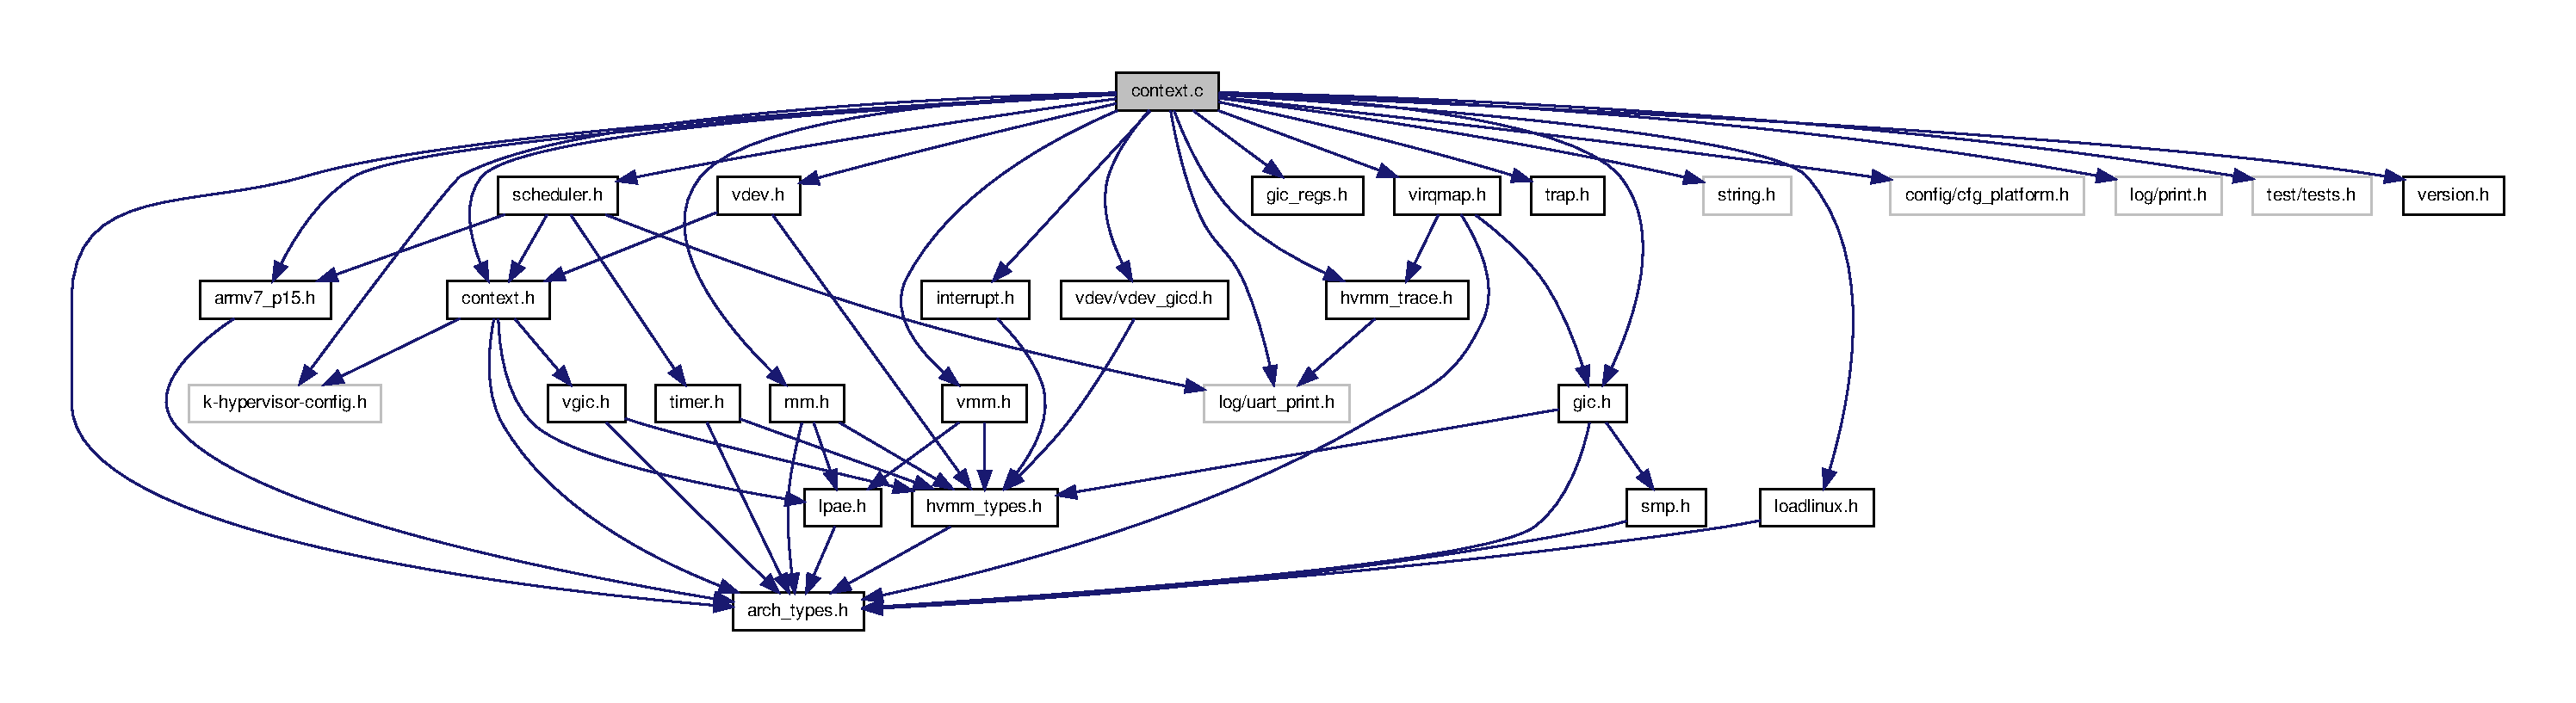
\includegraphics[width=350pt]{context_8c__incl}
\end{center}
\end{figure}
\subsection*{\-Defines}
\begin{DoxyCompactItemize}
\item 
\#define \hyperlink{context_8c_acf4405f8c387893e69eadc140804d0a4}{\-N\-U\-M\-\_\-\-G\-U\-E\-S\-T\-\_\-\-C\-O\-N\-T\-E\-X\-T\-S}~\hyperlink{hyp__config_8h_a7fcfcbc766cea81a21e2d8aba3b54843}{\-N\-U\-M\-\_\-\-G\-U\-E\-S\-T\-S\-\_\-\-S\-T\-A\-T\-I\-C}
\item 
\#define \hyperlink{context_8c_ac2acf5f304ad2586db8ac74f73583192}{\-C\-P\-S\-R\-\_\-\-M\-O\-D\-E\-\_\-\-U\-S\-E\-R}~0x10
\item 
\#define \hyperlink{context_8c_a60a6474fca8951df30ee82637a052343}{\-C\-P\-S\-R\-\_\-\-M\-O\-D\-E\-\_\-\-F\-I\-Q}~0x11
\item 
\#define \hyperlink{context_8c_a08f87658898e94f8dd95e9c5399e4b9f}{\-C\-P\-S\-R\-\_\-\-M\-O\-D\-E\-\_\-\-I\-R\-Q}~0x12
\item 
\#define \hyperlink{context_8c_a22cbc694995e613968671515fed868e3}{\-C\-P\-S\-R\-\_\-\-M\-O\-D\-E\-\_\-\-S\-V\-C}~0x13
\item 
\#define \hyperlink{context_8c_a09e3f1abdea736a92287ad2e6e34b140}{\-C\-P\-S\-R\-\_\-\-M\-O\-D\-E\-\_\-\-M\-O\-N}~0x16
\item 
\#define \hyperlink{context_8c_a9ba0ca5c2cb76845b52e65858e685aa0}{\-C\-P\-S\-R\-\_\-\-M\-O\-D\-E\-\_\-\-A\-B\-T}~0x17
\item 
\#define \hyperlink{context_8c_a8ea2c78389eb5876f60019865169ec9b}{\-C\-P\-S\-R\-\_\-\-M\-O\-D\-E\-\_\-\-H\-Y\-P}~0x1\-A
\item 
\#define \hyperlink{context_8c_ab9d61d021a43fac1fe42e6aafd2d79b4}{\-C\-P\-S\-R\-\_\-\-M\-O\-D\-E\-\_\-\-U\-N\-D}~0x1\-B
\item 
\#define \hyperlink{context_8c_a482d96e0df0946aa10ec155ae5284c43}{\-C\-P\-S\-R\-\_\-\-M\-O\-D\-E\-\_\-\-S\-Y\-S}~0x1\-F
\item 
\#define \hyperlink{context_8c_a53af5b93b8ac73356843a760d8b31944}{\-\_\-\-\_\-\-C\-O\-N\-T\-E\-X\-T\-\_\-\-T\-R\-A\-C\-E\-\_\-\-V\-E\-R\-B\-O\-S\-E\-\_\-\-\_\-}
\item 
\#define \hyperlink{context_8c_a6523708467fd815ab3dad9638219c7c2}{\-\_\-valid\-\_\-vmid}(vmid)~( \hyperlink{context_8h_a891f8f7028b04322da205990de1a8f5b}{context\-\_\-first\-\_\-vmid}() $<$= vmid \&\& \hyperlink{context_8h_ad48a9977fdb537cc020b451e08dfc590}{context\-\_\-last\-\_\-vmid}() $>$= vmid )
\end{DoxyCompactItemize}
\subsection*{\-Functions}
\begin{DoxyCompactItemize}
\item 
void \hyperlink{context_8c_a86f464d89297ef8121c2f36141c221a7}{\-\_\-\-\_\-mon\-\_\-switch\-\_\-to\-\_\-guest\-\_\-context} (struct \hyperlink{structarch__regs}{arch\-\_\-regs} $\ast$\hyperlink{vdev__timer_8c_a514d7f36beee4b3e39da305e12d39d0a}{regs})
\item 
static void \hyperlink{context_8c_a3a2da2487bde91bb02d3363bd17d905a}{\-\_\-hyp\-\_\-guest0\-\_\-copy\-\_\-zimage} (void)
\item 
void \hyperlink{context_8c_aa662295d6861cedca861f13c4ad5ece4}{context\-\_\-dump\-\_\-regs} (struct \hyperlink{structarch__regs}{arch\-\_\-regs} $\ast$\hyperlink{vdev__timer_8c_a514d7f36beee4b3e39da305e12d39d0a}{regs})
\item 
static void \hyperlink{context_8c_a58e0589f3c325fe4e8cd8cdd215d1e8b}{context\-\_\-copy\-\_\-regs} (struct \hyperlink{structarch__regs}{arch\-\_\-regs} $\ast$regs\-\_\-dst, struct \hyperlink{structarch__regs}{arch\-\_\-regs} $\ast$regs\-\_\-src)
\item 
void \hyperlink{context_8c_a6daf5c209647b93b848801070e6e30ef}{context\-\_\-init\-\_\-banked} (struct \hyperlink{structarch__regs__banked}{arch\-\_\-regs\-\_\-banked} $\ast$regs\-\_\-banked)
\item 
void \hyperlink{context_8c_a57af844ae7e83a33d88a4c36eee930eb}{context\-\_\-save\-\_\-banked} (struct \hyperlink{structarch__regs__banked}{arch\-\_\-regs\-\_\-banked} $\ast$regs\-\_\-banked)
\item 
void \hyperlink{context_8c_a94bb8d6785586134cc873c061076d323}{context\-\_\-restore\-\_\-banked} (struct \hyperlink{structarch__regs__banked}{arch\-\_\-regs\-\_\-banked} $\ast$regs\-\_\-banked)
\item 
void \hyperlink{context_8c_a3b7e34c1497427e5fdcc9b059fb813be}{context\-\_\-init\-\_\-cops} (struct \hyperlink{structarch__regs__cop}{arch\-\_\-regs\-\_\-cop} $\ast$regs\-\_\-cop)
\item 
void \hyperlink{context_8c_a9a5bddd4742fe9c4cc8ee9fa50cf03bf}{context\-\_\-save\-\_\-cops} (struct \hyperlink{structarch__regs__cop}{arch\-\_\-regs\-\_\-cop} $\ast$regs\-\_\-cop)
\item 
void \hyperlink{context_8c_a2d3fdf44ea523c8f4978cf9c33107768}{context\-\_\-restore\-\_\-cops} (struct \hyperlink{structarch__regs__cop}{arch\-\_\-regs\-\_\-cop} $\ast$regs\-\_\-cop)
\item 
static \hyperlink{hvmm__types_8h_a39d593b2c97852f566d7472b76ab7ba2}{hvmm\-\_\-status\-\_\-t} \hyperlink{context_8c_adbcfdbfe8d61021879f1622e2c6dc29c}{context\-\_\-perform\-\_\-switch\-\_\-to\-\_\-guest\-\_\-regs} (struct \hyperlink{structarch__regs}{arch\-\_\-regs} $\ast$regs\-\_\-current, \hyperlink{hvmm__types_8h_af7e9bd0adfb7d10e7a7a0ee60a5f962c}{vmid\-\_\-t} next\-\_\-vmid)
\item 
\hyperlink{hvmm__types_8h_a39d593b2c97852f566d7472b76ab7ba2}{hvmm\-\_\-status\-\_\-t} \hyperlink{context_8c_a77fe269a194f9dcfcd0a599a9b6e3bfb}{context\-\_\-perform\-\_\-switch} (void)
\item 
void \hyperlink{context_8c_a39db644c82cc9c99ef78feb58d57b58c}{context\-\_\-switch\-\_\-to\-\_\-initial\-\_\-guest} (void)
\item 
void \hyperlink{context_8c_a0abdd106a2b654464230b622b4c9877e}{context\-\_\-init\-\_\-guests} (void)
\item 
struct \hyperlink{structhyp__guest__context}{hyp\-\_\-guest\-\_\-context} $\ast$ \hyperlink{context_8c_ae8e692844cf2c76f7661088f7a7be817}{context\-\_\-atvmid} (\hyperlink{hvmm__types_8h_af7e9bd0adfb7d10e7a7a0ee60a5f962c}{vmid\-\_\-t} vmid)
\item 
\hyperlink{hvmm__types_8h_af7e9bd0adfb7d10e7a7a0ee60a5f962c}{vmid\-\_\-t} \hyperlink{context_8c_a891f8f7028b04322da205990de1a8f5b}{context\-\_\-first\-\_\-vmid} (void)
\item 
\hyperlink{hvmm__types_8h_af7e9bd0adfb7d10e7a7a0ee60a5f962c}{vmid\-\_\-t} \hyperlink{context_8c_ad48a9977fdb537cc020b451e08dfc590}{context\-\_\-last\-\_\-vmid} (void)
\item 
\hyperlink{hvmm__types_8h_af7e9bd0adfb7d10e7a7a0ee60a5f962c}{vmid\-\_\-t} \hyperlink{context_8c_a5719d5d4a8d98b9784d0f24a2023f05f}{context\-\_\-next\-\_\-vmid} (\hyperlink{hvmm__types_8h_af7e9bd0adfb7d10e7a7a0ee60a5f962c}{vmid\-\_\-t} ofvmid)
\item 
\hyperlink{hvmm__types_8h_af7e9bd0adfb7d10e7a7a0ee60a5f962c}{vmid\-\_\-t} \hyperlink{context_8c_a525fcf860b6f33b4192443c9d66ba4f6}{context\-\_\-current\-\_\-vmid} (void)
\item 
\hyperlink{hvmm__types_8h_af7e9bd0adfb7d10e7a7a0ee60a5f962c}{vmid\-\_\-t} \hyperlink{context_8c_a3fd5aa68bf14823442fcc5fda4cb6a51}{context\-\_\-waiting\-\_\-vmid} (void)
\item 
\hyperlink{hvmm__types_8h_a39d593b2c97852f566d7472b76ab7ba2}{hvmm\-\_\-status\-\_\-t} \hyperlink{context_8c_aaa75f8a973764763b44ca823e02f4406}{context\-\_\-switchto} (\hyperlink{hvmm__types_8h_af7e9bd0adfb7d10e7a7a0ee60a5f962c}{vmid\-\_\-t} vmid)
\item 
\hyperlink{hvmm__types_8h_a39d593b2c97852f566d7472b76ab7ba2}{hvmm\-\_\-status\-\_\-t} \hyperlink{context_8c_a00b56df45d0ef16d93040b667bb025ef}{context\-\_\-switchto\-\_\-lock} (\hyperlink{hvmm__types_8h_af7e9bd0adfb7d10e7a7a0ee60a5f962c}{vmid\-\_\-t} vmid, \hyperlink{arch__types_8h_aba7bc1797add20fe3efdf37ced1182c5}{uint8\-\_\-t} locked)
\item 
void \hyperlink{context_8c_a83895de158b7efc9456e7475528e42d4}{start\-\_\-guest\-\_\-os} (void)
\end{DoxyCompactItemize}
\subsection*{\-Variables}
\begin{DoxyCompactItemize}
\item 
static struct \hyperlink{structhyp__guest__context}{hyp\-\_\-guest\-\_\-context} \hyperlink{context_8c_a7a55b222a2790b315eaf5dbe7a12c407}{guest\-\_\-contexts} \mbox{[}\hyperlink{context_8c_acf4405f8c387893e69eadc140804d0a4}{\-N\-U\-M\-\_\-\-G\-U\-E\-S\-T\-\_\-\-C\-O\-N\-T\-E\-X\-T\-S}\mbox{]}
\item 
static int \hyperlink{context_8c_a5de72a0d4dd972c7d7d8c9d08272d9e8}{\-\_\-current\-\_\-guest\-\_\-vmid} = \hyperlink{hvmm__types_8h_a286d5f39683a49a6e5d4ef92043b3c9f}{\-V\-M\-I\-D\-\_\-\-I\-N\-V\-A\-L\-I\-D}
\item 
static int \hyperlink{context_8c_a5f1b0bb9a3d788646bb83d32d12419f3}{\-\_\-next\-\_\-guest\-\_\-vmid} = \hyperlink{hvmm__types_8h_a286d5f39683a49a6e5d4ef92043b3c9f}{\-V\-M\-I\-D\-\_\-\-I\-N\-V\-A\-L\-I\-D}
\item 
static \hyperlink{arch__types_8h_aba7bc1797add20fe3efdf37ced1182c5}{uint8\-\_\-t} \hyperlink{context_8c_a345440f03deca2090efe13b08eaead89}{\-\_\-switch\-\_\-locked} = 0
\end{DoxyCompactItemize}


\subsection{\-Define \-Documentation}
\hypertarget{context_8c_a53af5b93b8ac73356843a760d8b31944}{\index{context.\-c@{context.\-c}!\-\_\-\-\_\-\-C\-O\-N\-T\-E\-X\-T\-\_\-\-T\-R\-A\-C\-E\-\_\-\-V\-E\-R\-B\-O\-S\-E\-\_\-\-\_\-@{\-\_\-\-\_\-\-C\-O\-N\-T\-E\-X\-T\-\_\-\-T\-R\-A\-C\-E\-\_\-\-V\-E\-R\-B\-O\-S\-E\-\_\-\-\_\-}}
\index{\-\_\-\-\_\-\-C\-O\-N\-T\-E\-X\-T\-\_\-\-T\-R\-A\-C\-E\-\_\-\-V\-E\-R\-B\-O\-S\-E\-\_\-\-\_\-@{\-\_\-\-\_\-\-C\-O\-N\-T\-E\-X\-T\-\_\-\-T\-R\-A\-C\-E\-\_\-\-V\-E\-R\-B\-O\-S\-E\-\_\-\-\_\-}!context.c@{context.\-c}}
\subsubsection[{\-\_\-\-\_\-\-C\-O\-N\-T\-E\-X\-T\-\_\-\-T\-R\-A\-C\-E\-\_\-\-V\-E\-R\-B\-O\-S\-E\-\_\-\-\_\-}]{\setlength{\rightskip}{0pt plus 5cm}\#define {\bf \-\_\-\-\_\-\-C\-O\-N\-T\-E\-X\-T\-\_\-\-T\-R\-A\-C\-E\-\_\-\-V\-E\-R\-B\-O\-S\-E\-\_\-\-\_\-}}}\label{context_8c_a53af5b93b8ac73356843a760d8b31944}


\-Definition at line 44 of file context.\-c.

\hypertarget{context_8c_a6523708467fd815ab3dad9638219c7c2}{\index{context.\-c@{context.\-c}!\-\_\-valid\-\_\-vmid@{\-\_\-valid\-\_\-vmid}}
\index{\-\_\-valid\-\_\-vmid@{\-\_\-valid\-\_\-vmid}!context.c@{context.\-c}}
\subsubsection[{\-\_\-valid\-\_\-vmid}]{\setlength{\rightskip}{0pt plus 5cm}\#define {\bf \-\_\-valid\-\_\-vmid}(
\begin{DoxyParamCaption}
\item[{}]{vmid}
\end{DoxyParamCaption}
)~( {\bf context\-\_\-first\-\_\-vmid}() $<$= vmid \&\& {\bf context\-\_\-last\-\_\-vmid}() $>$= vmid )}}\label{context_8c_a6523708467fd815ab3dad9638219c7c2}


\-Definition at line 45 of file context.\-c.

\hypertarget{context_8c_a9ba0ca5c2cb76845b52e65858e685aa0}{\index{context.\-c@{context.\-c}!\-C\-P\-S\-R\-\_\-\-M\-O\-D\-E\-\_\-\-A\-B\-T@{\-C\-P\-S\-R\-\_\-\-M\-O\-D\-E\-\_\-\-A\-B\-T}}
\index{\-C\-P\-S\-R\-\_\-\-M\-O\-D\-E\-\_\-\-A\-B\-T@{\-C\-P\-S\-R\-\_\-\-M\-O\-D\-E\-\_\-\-A\-B\-T}!context.c@{context.\-c}}
\subsubsection[{\-C\-P\-S\-R\-\_\-\-M\-O\-D\-E\-\_\-\-A\-B\-T}]{\setlength{\rightskip}{0pt plus 5cm}\#define {\bf \-C\-P\-S\-R\-\_\-\-M\-O\-D\-E\-\_\-\-A\-B\-T}~0x17}}\label{context_8c_a9ba0ca5c2cb76845b52e65858e685aa0}


\-Definition at line 39 of file context.\-c.

\hypertarget{context_8c_a60a6474fca8951df30ee82637a052343}{\index{context.\-c@{context.\-c}!\-C\-P\-S\-R\-\_\-\-M\-O\-D\-E\-\_\-\-F\-I\-Q@{\-C\-P\-S\-R\-\_\-\-M\-O\-D\-E\-\_\-\-F\-I\-Q}}
\index{\-C\-P\-S\-R\-\_\-\-M\-O\-D\-E\-\_\-\-F\-I\-Q@{\-C\-P\-S\-R\-\_\-\-M\-O\-D\-E\-\_\-\-F\-I\-Q}!context.c@{context.\-c}}
\subsubsection[{\-C\-P\-S\-R\-\_\-\-M\-O\-D\-E\-\_\-\-F\-I\-Q}]{\setlength{\rightskip}{0pt plus 5cm}\#define {\bf \-C\-P\-S\-R\-\_\-\-M\-O\-D\-E\-\_\-\-F\-I\-Q}~0x11}}\label{context_8c_a60a6474fca8951df30ee82637a052343}


\-Definition at line 35 of file context.\-c.

\hypertarget{context_8c_a8ea2c78389eb5876f60019865169ec9b}{\index{context.\-c@{context.\-c}!\-C\-P\-S\-R\-\_\-\-M\-O\-D\-E\-\_\-\-H\-Y\-P@{\-C\-P\-S\-R\-\_\-\-M\-O\-D\-E\-\_\-\-H\-Y\-P}}
\index{\-C\-P\-S\-R\-\_\-\-M\-O\-D\-E\-\_\-\-H\-Y\-P@{\-C\-P\-S\-R\-\_\-\-M\-O\-D\-E\-\_\-\-H\-Y\-P}!context.c@{context.\-c}}
\subsubsection[{\-C\-P\-S\-R\-\_\-\-M\-O\-D\-E\-\_\-\-H\-Y\-P}]{\setlength{\rightskip}{0pt plus 5cm}\#define {\bf \-C\-P\-S\-R\-\_\-\-M\-O\-D\-E\-\_\-\-H\-Y\-P}~0x1\-A}}\label{context_8c_a8ea2c78389eb5876f60019865169ec9b}


\-Definition at line 40 of file context.\-c.

\hypertarget{context_8c_a08f87658898e94f8dd95e9c5399e4b9f}{\index{context.\-c@{context.\-c}!\-C\-P\-S\-R\-\_\-\-M\-O\-D\-E\-\_\-\-I\-R\-Q@{\-C\-P\-S\-R\-\_\-\-M\-O\-D\-E\-\_\-\-I\-R\-Q}}
\index{\-C\-P\-S\-R\-\_\-\-M\-O\-D\-E\-\_\-\-I\-R\-Q@{\-C\-P\-S\-R\-\_\-\-M\-O\-D\-E\-\_\-\-I\-R\-Q}!context.c@{context.\-c}}
\subsubsection[{\-C\-P\-S\-R\-\_\-\-M\-O\-D\-E\-\_\-\-I\-R\-Q}]{\setlength{\rightskip}{0pt plus 5cm}\#define {\bf \-C\-P\-S\-R\-\_\-\-M\-O\-D\-E\-\_\-\-I\-R\-Q}~0x12}}\label{context_8c_a08f87658898e94f8dd95e9c5399e4b9f}


\-Definition at line 36 of file context.\-c.

\hypertarget{context_8c_a09e3f1abdea736a92287ad2e6e34b140}{\index{context.\-c@{context.\-c}!\-C\-P\-S\-R\-\_\-\-M\-O\-D\-E\-\_\-\-M\-O\-N@{\-C\-P\-S\-R\-\_\-\-M\-O\-D\-E\-\_\-\-M\-O\-N}}
\index{\-C\-P\-S\-R\-\_\-\-M\-O\-D\-E\-\_\-\-M\-O\-N@{\-C\-P\-S\-R\-\_\-\-M\-O\-D\-E\-\_\-\-M\-O\-N}!context.c@{context.\-c}}
\subsubsection[{\-C\-P\-S\-R\-\_\-\-M\-O\-D\-E\-\_\-\-M\-O\-N}]{\setlength{\rightskip}{0pt plus 5cm}\#define {\bf \-C\-P\-S\-R\-\_\-\-M\-O\-D\-E\-\_\-\-M\-O\-N}~0x16}}\label{context_8c_a09e3f1abdea736a92287ad2e6e34b140}


\-Definition at line 38 of file context.\-c.

\hypertarget{context_8c_a22cbc694995e613968671515fed868e3}{\index{context.\-c@{context.\-c}!\-C\-P\-S\-R\-\_\-\-M\-O\-D\-E\-\_\-\-S\-V\-C@{\-C\-P\-S\-R\-\_\-\-M\-O\-D\-E\-\_\-\-S\-V\-C}}
\index{\-C\-P\-S\-R\-\_\-\-M\-O\-D\-E\-\_\-\-S\-V\-C@{\-C\-P\-S\-R\-\_\-\-M\-O\-D\-E\-\_\-\-S\-V\-C}!context.c@{context.\-c}}
\subsubsection[{\-C\-P\-S\-R\-\_\-\-M\-O\-D\-E\-\_\-\-S\-V\-C}]{\setlength{\rightskip}{0pt plus 5cm}\#define {\bf \-C\-P\-S\-R\-\_\-\-M\-O\-D\-E\-\_\-\-S\-V\-C}~0x13}}\label{context_8c_a22cbc694995e613968671515fed868e3}


\-Definition at line 37 of file context.\-c.

\hypertarget{context_8c_a482d96e0df0946aa10ec155ae5284c43}{\index{context.\-c@{context.\-c}!\-C\-P\-S\-R\-\_\-\-M\-O\-D\-E\-\_\-\-S\-Y\-S@{\-C\-P\-S\-R\-\_\-\-M\-O\-D\-E\-\_\-\-S\-Y\-S}}
\index{\-C\-P\-S\-R\-\_\-\-M\-O\-D\-E\-\_\-\-S\-Y\-S@{\-C\-P\-S\-R\-\_\-\-M\-O\-D\-E\-\_\-\-S\-Y\-S}!context.c@{context.\-c}}
\subsubsection[{\-C\-P\-S\-R\-\_\-\-M\-O\-D\-E\-\_\-\-S\-Y\-S}]{\setlength{\rightskip}{0pt plus 5cm}\#define {\bf \-C\-P\-S\-R\-\_\-\-M\-O\-D\-E\-\_\-\-S\-Y\-S}~0x1\-F}}\label{context_8c_a482d96e0df0946aa10ec155ae5284c43}


\-Definition at line 42 of file context.\-c.

\hypertarget{context_8c_ab9d61d021a43fac1fe42e6aafd2d79b4}{\index{context.\-c@{context.\-c}!\-C\-P\-S\-R\-\_\-\-M\-O\-D\-E\-\_\-\-U\-N\-D@{\-C\-P\-S\-R\-\_\-\-M\-O\-D\-E\-\_\-\-U\-N\-D}}
\index{\-C\-P\-S\-R\-\_\-\-M\-O\-D\-E\-\_\-\-U\-N\-D@{\-C\-P\-S\-R\-\_\-\-M\-O\-D\-E\-\_\-\-U\-N\-D}!context.c@{context.\-c}}
\subsubsection[{\-C\-P\-S\-R\-\_\-\-M\-O\-D\-E\-\_\-\-U\-N\-D}]{\setlength{\rightskip}{0pt plus 5cm}\#define {\bf \-C\-P\-S\-R\-\_\-\-M\-O\-D\-E\-\_\-\-U\-N\-D}~0x1\-B}}\label{context_8c_ab9d61d021a43fac1fe42e6aafd2d79b4}


\-Definition at line 41 of file context.\-c.

\hypertarget{context_8c_ac2acf5f304ad2586db8ac74f73583192}{\index{context.\-c@{context.\-c}!\-C\-P\-S\-R\-\_\-\-M\-O\-D\-E\-\_\-\-U\-S\-E\-R@{\-C\-P\-S\-R\-\_\-\-M\-O\-D\-E\-\_\-\-U\-S\-E\-R}}
\index{\-C\-P\-S\-R\-\_\-\-M\-O\-D\-E\-\_\-\-U\-S\-E\-R@{\-C\-P\-S\-R\-\_\-\-M\-O\-D\-E\-\_\-\-U\-S\-E\-R}!context.c@{context.\-c}}
\subsubsection[{\-C\-P\-S\-R\-\_\-\-M\-O\-D\-E\-\_\-\-U\-S\-E\-R}]{\setlength{\rightskip}{0pt plus 5cm}\#define {\bf \-C\-P\-S\-R\-\_\-\-M\-O\-D\-E\-\_\-\-U\-S\-E\-R}~0x10}}\label{context_8c_ac2acf5f304ad2586db8ac74f73583192}


\-Definition at line 34 of file context.\-c.

\hypertarget{context_8c_acf4405f8c387893e69eadc140804d0a4}{\index{context.\-c@{context.\-c}!\-N\-U\-M\-\_\-\-G\-U\-E\-S\-T\-\_\-\-C\-O\-N\-T\-E\-X\-T\-S@{\-N\-U\-M\-\_\-\-G\-U\-E\-S\-T\-\_\-\-C\-O\-N\-T\-E\-X\-T\-S}}
\index{\-N\-U\-M\-\_\-\-G\-U\-E\-S\-T\-\_\-\-C\-O\-N\-T\-E\-X\-T\-S@{\-N\-U\-M\-\_\-\-G\-U\-E\-S\-T\-\_\-\-C\-O\-N\-T\-E\-X\-T\-S}!context.c@{context.\-c}}
\subsubsection[{\-N\-U\-M\-\_\-\-G\-U\-E\-S\-T\-\_\-\-C\-O\-N\-T\-E\-X\-T\-S}]{\setlength{\rightskip}{0pt plus 5cm}\#define {\bf \-N\-U\-M\-\_\-\-G\-U\-E\-S\-T\-\_\-\-C\-O\-N\-T\-E\-X\-T\-S}~{\bf \-N\-U\-M\-\_\-\-G\-U\-E\-S\-T\-S\-\_\-\-S\-T\-A\-T\-I\-C}}}\label{context_8c_acf4405f8c387893e69eadc140804d0a4}


\-Definition at line 32 of file context.\-c.



\subsection{\-Function \-Documentation}
\hypertarget{context_8c_a86f464d89297ef8121c2f36141c221a7}{\index{context.\-c@{context.\-c}!\-\_\-\-\_\-mon\-\_\-switch\-\_\-to\-\_\-guest\-\_\-context@{\-\_\-\-\_\-mon\-\_\-switch\-\_\-to\-\_\-guest\-\_\-context}}
\index{\-\_\-\-\_\-mon\-\_\-switch\-\_\-to\-\_\-guest\-\_\-context@{\-\_\-\-\_\-mon\-\_\-switch\-\_\-to\-\_\-guest\-\_\-context}!context.c@{context.\-c}}
\subsubsection[{\-\_\-\-\_\-mon\-\_\-switch\-\_\-to\-\_\-guest\-\_\-context}]{\setlength{\rightskip}{0pt plus 5cm}void {\bf \-\_\-\-\_\-mon\-\_\-switch\-\_\-to\-\_\-guest\-\_\-context} (
\begin{DoxyParamCaption}
\item[{struct {\bf arch\-\_\-regs} $\ast$}]{regs}
\end{DoxyParamCaption}
)}}\label{context_8c_a86f464d89297ef8121c2f36141c221a7}
\hypertarget{context_8c_a3a2da2487bde91bb02d3363bd17d905a}{\index{context.\-c@{context.\-c}!\-\_\-hyp\-\_\-guest0\-\_\-copy\-\_\-zimage@{\-\_\-hyp\-\_\-guest0\-\_\-copy\-\_\-zimage}}
\index{\-\_\-hyp\-\_\-guest0\-\_\-copy\-\_\-zimage@{\-\_\-hyp\-\_\-guest0\-\_\-copy\-\_\-zimage}!context.c@{context.\-c}}
\subsubsection[{\-\_\-hyp\-\_\-guest0\-\_\-copy\-\_\-zimage}]{\setlength{\rightskip}{0pt plus 5cm}static void {\bf \-\_\-hyp\-\_\-guest0\-\_\-copy\-\_\-zimage} (
\begin{DoxyParamCaption}
\item[{void}]{}
\end{DoxyParamCaption}
)\hspace{0.3cm}{\ttfamily  \mbox{[}static\mbox{]}}}}\label{context_8c_a3a2da2487bde91bb02d3363bd17d905a}


\-Definition at line 59 of file context.\-c.


\begin{DoxyCode}
{
    extern uint32_t guest_bin_start;
    extern uint32_t guest_bin_end;

    uint32_t *src = &guest_bin_start;
    uint32_t *end = &guest_bin_end;
    uint32_t *dst = &guest_bin_start + (0x20008000/4);

    HVMM_TRACE_ENTER();

    uart_print("Copying guest0 image to guest1\n\r");
    uart_print(" src:");uart_print_hex32((uint32_t)src); 
    uart_print(" dst:");uart_print_hex32((uint32_t)dst); 
    uart_print(" size:");uart_print_hex32( (uint32_t)(end - src) * sizeof(
      uint32_t));uart_print("\n\r");

    while(src < end ) {
        *dst++ = *src++;
    }
    uart_print("=== done ===\n\r");
    HVMM_TRACE_EXIT();
}
\end{DoxyCode}
\hypertarget{context_8c_ae8e692844cf2c76f7661088f7a7be817}{\index{context.\-c@{context.\-c}!context\-\_\-atvmid@{context\-\_\-atvmid}}
\index{context\-\_\-atvmid@{context\-\_\-atvmid}!context.c@{context.\-c}}
\subsubsection[{context\-\_\-atvmid}]{\setlength{\rightskip}{0pt plus 5cm}struct {\bf hyp\-\_\-guest\-\_\-context}$\ast$ {\bf context\-\_\-atvmid} (
\begin{DoxyParamCaption}
\item[{{\bf vmid\-\_\-t}}]{vmid}
\end{DoxyParamCaption}
)\hspace{0.3cm}{\ttfamily  \mbox{[}read\mbox{]}}}}\label{context_8c_ae8e692844cf2c76f7661088f7a7be817}


\-Definition at line 526 of file context.\-c.


\begin{DoxyCode}
{
    struct hyp_guest_context * result = 0;

    if ( vmid < NUM_GUEST_CONTEXTS ) {
        result = &guest_contexts[vmid];
    }

    return result;
}
\end{DoxyCode}
\hypertarget{context_8c_a58e0589f3c325fe4e8cd8cdd215d1e8b}{\index{context.\-c@{context.\-c}!context\-\_\-copy\-\_\-regs@{context\-\_\-copy\-\_\-regs}}
\index{context\-\_\-copy\-\_\-regs@{context\-\_\-copy\-\_\-regs}!context.c@{context.\-c}}
\subsubsection[{context\-\_\-copy\-\_\-regs}]{\setlength{\rightskip}{0pt plus 5cm}static void {\bf context\-\_\-copy\-\_\-regs} (
\begin{DoxyParamCaption}
\item[{struct {\bf arch\-\_\-regs} $\ast$}]{regs\-\_\-dst, }
\item[{struct {\bf arch\-\_\-regs} $\ast$}]{regs\-\_\-src}
\end{DoxyParamCaption}
)\hspace{0.3cm}{\ttfamily  \mbox{[}static\mbox{]}}}}\label{context_8c_a58e0589f3c325fe4e8cd8cdd215d1e8b}


\-Definition at line 163 of file context.\-c.


\begin{DoxyCode}
{
    int i;
    regs_dst->cpsr = regs_src->cpsr;
    regs_dst->pc = regs_src->pc;
    regs_dst->lr = regs_src->lr;
    for( i = 0; i < ARCH_REGS_NUM_GPR; i++) {
        regs_dst->gpr[i] = regs_src->gpr[i];
    }
}
\end{DoxyCode}
\hypertarget{context_8c_a525fcf860b6f33b4192443c9d66ba4f6}{\index{context.\-c@{context.\-c}!context\-\_\-current\-\_\-vmid@{context\-\_\-current\-\_\-vmid}}
\index{context\-\_\-current\-\_\-vmid@{context\-\_\-current\-\_\-vmid}!context.c@{context.\-c}}
\subsubsection[{context\-\_\-current\-\_\-vmid}]{\setlength{\rightskip}{0pt plus 5cm}{\bf vmid\-\_\-t} {\bf context\-\_\-current\-\_\-vmid} (
\begin{DoxyParamCaption}
\item[{void}]{}
\end{DoxyParamCaption}
)}}\label{context_8c_a525fcf860b6f33b4192443c9d66ba4f6}


\-Definition at line 562 of file context.\-c.


\begin{DoxyCode}
{
    return _current_guest_vmid;
}
\end{DoxyCode}
\hypertarget{context_8c_aa662295d6861cedca861f13c4ad5ece4}{\index{context.\-c@{context.\-c}!context\-\_\-dump\-\_\-regs@{context\-\_\-dump\-\_\-regs}}
\index{context\-\_\-dump\-\_\-regs@{context\-\_\-dump\-\_\-regs}!context.c@{context.\-c}}
\subsubsection[{context\-\_\-dump\-\_\-regs}]{\setlength{\rightskip}{0pt plus 5cm}void {\bf context\-\_\-dump\-\_\-regs} (
\begin{DoxyParamCaption}
\item[{struct {\bf arch\-\_\-regs} $\ast$}]{regs}
\end{DoxyParamCaption}
)}}\label{context_8c_aa662295d6861cedca861f13c4ad5ece4}


\-Definition at line 145 of file context.\-c.


\begin{DoxyCode}
{
#ifdef DEBUG
    uart_print( "cpsr:" ); uart_print_hex32( regs->cpsr ); uart_print( "\n\r" )
      ;
    uart_print( "  pc:" ); uart_print_hex32( regs->pc ); uart_print( "\n\r" );
    uart_print( "  lr:" ); uart_print_hex32( regs->lr ); uart_print( "\n\r" );

#ifdef __CONTEXT_TRACE_VERBOSE__
    {
        int i;
        uart_print( " gpr:\n\r" );
        for( i = 0; i < ARCH_REGS_NUM_GPR; i++) {
            uart_print( "     " ); uart_print_hex32( regs->gpr[i] ); uart_print
      ( "\n\r" );
        }
    }
#endif
#endif
}
\end{DoxyCode}
\hypertarget{context_8c_a891f8f7028b04322da205990de1a8f5b}{\index{context.\-c@{context.\-c}!context\-\_\-first\-\_\-vmid@{context\-\_\-first\-\_\-vmid}}
\index{context\-\_\-first\-\_\-vmid@{context\-\_\-first\-\_\-vmid}!context.c@{context.\-c}}
\subsubsection[{context\-\_\-first\-\_\-vmid}]{\setlength{\rightskip}{0pt plus 5cm}{\bf vmid\-\_\-t} {\bf context\-\_\-first\-\_\-vmid} (
\begin{DoxyParamCaption}
\item[{void}]{}
\end{DoxyParamCaption}
)}}\label{context_8c_a891f8f7028b04322da205990de1a8f5b}


\-Definition at line 538 of file context.\-c.


\begin{DoxyCode}
{
    /* FIXME:Hardcoded for now */
    return 0;
}
\end{DoxyCode}
\hypertarget{context_8c_a6daf5c209647b93b848801070e6e30ef}{\index{context.\-c@{context.\-c}!context\-\_\-init\-\_\-banked@{context\-\_\-init\-\_\-banked}}
\index{context\-\_\-init\-\_\-banked@{context\-\_\-init\-\_\-banked}!context.c@{context.\-c}}
\subsubsection[{context\-\_\-init\-\_\-banked}]{\setlength{\rightskip}{0pt plus 5cm}void {\bf context\-\_\-init\-\_\-banked} (
\begin{DoxyParamCaption}
\item[{struct {\bf arch\-\_\-regs\-\_\-banked} $\ast$}]{regs\-\_\-banked}
\end{DoxyParamCaption}
)}}\label{context_8c_a6daf5c209647b93b848801070e6e30ef}


\-Definition at line 176 of file context.\-c.


\begin{DoxyCode}
{
    regs_banked->sp_usr = 0;
    regs_banked->spsr_svc = 0;
    regs_banked->sp_svc = 0;
    regs_banked->lr_svc = 0;
    regs_banked->spsr_abt = 0;
    regs_banked->sp_abt = 0;
    regs_banked->lr_abt = 0;
    regs_banked->spsr_und = 0;
    regs_banked->sp_und = 0;
    regs_banked->lr_und = 0;
    regs_banked->spsr_irq = 0;
    regs_banked->sp_irq = 0;
    regs_banked->lr_irq = 0;
    regs_banked->spsr_fiq = 0;
    regs_banked->lr_fiq = 0;
    regs_banked->r8_fiq = 0;
    regs_banked->r9_fiq = 0;
    regs_banked->r10_fiq = 0;
    regs_banked->r11_fiq = 0;
    regs_banked->r12_fiq = 0;
    //Cortex-A15 processor does not support sp_fiq
}
\end{DoxyCode}
\hypertarget{context_8c_a3b7e34c1497427e5fdcc9b059fb813be}{\index{context.\-c@{context.\-c}!context\-\_\-init\-\_\-cops@{context\-\_\-init\-\_\-cops}}
\index{context\-\_\-init\-\_\-cops@{context\-\_\-init\-\_\-cops}!context.c@{context.\-c}}
\subsubsection[{context\-\_\-init\-\_\-cops}]{\setlength{\rightskip}{0pt plus 5cm}void {\bf context\-\_\-init\-\_\-cops} (
\begin{DoxyParamCaption}
\item[{struct {\bf arch\-\_\-regs\-\_\-cop} $\ast$}]{regs\-\_\-cop}
\end{DoxyParamCaption}
)}}\label{context_8c_a3b7e34c1497427e5fdcc9b059fb813be}


\-Definition at line 313 of file context.\-c.


\begin{DoxyCode}
{
    regs_cop->vbar = 0;
    regs_cop->ttbr0 = 0;
    regs_cop->ttbr1 = 0;
    regs_cop->ttbcr = 0;
    regs_cop->sctlr = 0;
}
\end{DoxyCode}
\hypertarget{context_8c_a0abdd106a2b654464230b622b4c9877e}{\index{context.\-c@{context.\-c}!context\-\_\-init\-\_\-guests@{context\-\_\-init\-\_\-guests}}
\index{context\-\_\-init\-\_\-guests@{context\-\_\-init\-\_\-guests}!context.c@{context.\-c}}
\subsubsection[{context\-\_\-init\-\_\-guests}]{\setlength{\rightskip}{0pt plus 5cm}void {\bf context\-\_\-init\-\_\-guests} (
\begin{DoxyParamCaption}
\item[{void}]{}
\end{DoxyParamCaption}
)}}\label{context_8c_a0abdd106a2b654464230b622b4c9877e}


\-Definition at line 468 of file context.\-c.


\begin{DoxyCode}
{
    struct hyp_guest_context *context;
    struct arch_regs *regs = 0;

    
    uart_print("[hyp] init_guests: enter\n\r");


    /* Guest 1 @guest_bin_start */
    context = &guest_contexts[0];
    regs = &context->regs;
    regs->cpsr = 0x1d3;         // supervisor, interrupt disabled
#if defined (LINUX_GUEST)
    regs->pc = 0xA0008000;      // PA:0xA0008000, where zImage is
    regs->gpr[1] = CFG_MACHINE_NUMBER;
    regs->gpr[2] = 0x80000100;  //src+(0x100/4);
#else
    regs->pc = 0x80000000;      // PA:0xA0000000, default entry for bmguest
#endif

    /* regs->gpr[] = whatever */
    context->vmid = 0;
    context->ttbl = vmm_vmid_ttbl(context->vmid);
    context_init_cops( &context->regs_cop );
    context_init_banked( &context->regs_banked );
    vgic_init_status( &context->vgic_status, context->vmid );

    /* Guest 2 @guest2_bin_start */
    context = &guest_contexts[1];
    regs = &context->regs;
    regs->pc = 0x80000000;  // PA: 0xB0000000
    regs->cpsr = 0x1d3; // supervisor, interrupt disabled

    /* regs->gpr[] = whatever */
    context->vmid = 1;
    context->ttbl = vmm_vmid_ttbl(context->vmid);
    context_init_cops( &context->regs_cop );
    context_init_banked( &context->regs_banked );
    vgic_init_status( &context->vgic_status, context->vmid );

#if defined (LINUX_GUEST)
    _hyp_guest0_copy_zimage();
#elif defined (BAREMETAL_GUEST) 
    /* Workaround for unloaded bmguest.bin at 0xB0000000@PA */
    _hyp_fixup_unloaded_guest();
#endif

#if defined (LINUX_GUEST)
    {
        extern uint32_t guest_bin_start;
        uint32_t *src = &guest_bin_start;
        loadlinux_setup_tags(src);
    }
#endif
    uart_print("[hyp] init_guests: return\n\r");
}
\end{DoxyCode}


\-Here is the call graph for this function\-:
\nopagebreak
\begin{figure}[H]
\begin{center}
\leavevmode
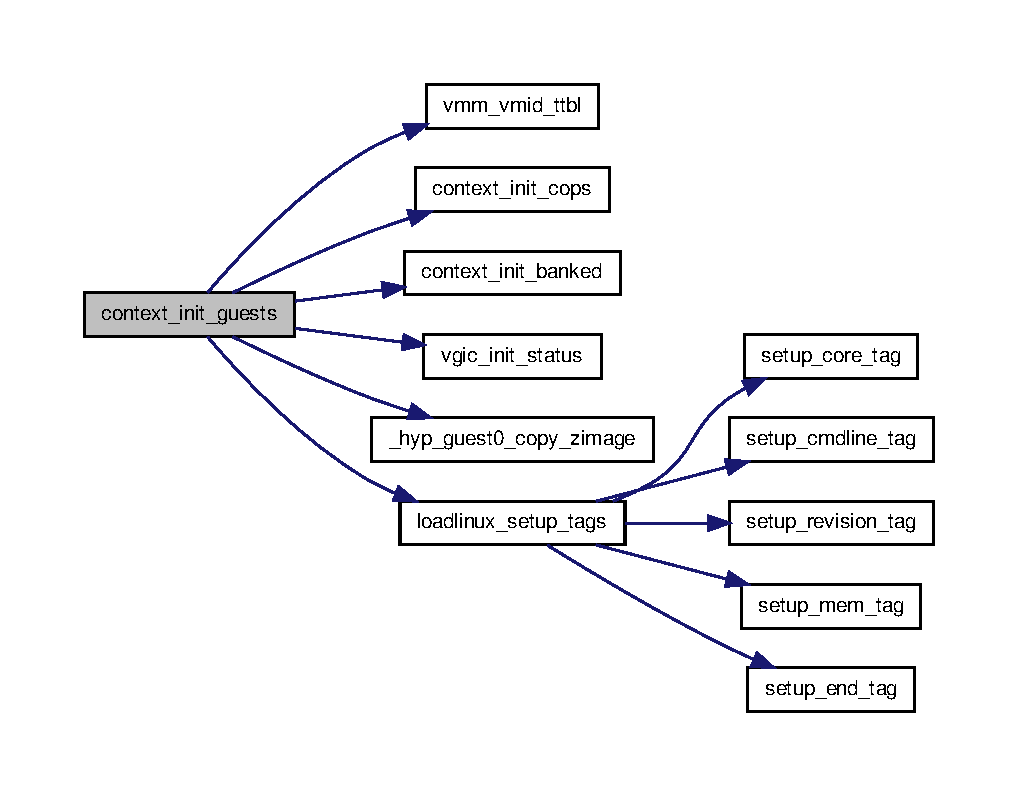
\includegraphics[width=350pt]{context_8c_a0abdd106a2b654464230b622b4c9877e_cgraph}
\end{center}
\end{figure}


\hypertarget{context_8c_ad48a9977fdb537cc020b451e08dfc590}{\index{context.\-c@{context.\-c}!context\-\_\-last\-\_\-vmid@{context\-\_\-last\-\_\-vmid}}
\index{context\-\_\-last\-\_\-vmid@{context\-\_\-last\-\_\-vmid}!context.c@{context.\-c}}
\subsubsection[{context\-\_\-last\-\_\-vmid}]{\setlength{\rightskip}{0pt plus 5cm}{\bf vmid\-\_\-t} {\bf context\-\_\-last\-\_\-vmid} (
\begin{DoxyParamCaption}
\item[{void}]{}
\end{DoxyParamCaption}
)}}\label{context_8c_ad48a9977fdb537cc020b451e08dfc590}


\-Definition at line 544 of file context.\-c.


\begin{DoxyCode}
{
    /* FIXME:Hardcoded for now */
    return 1;
}
\end{DoxyCode}
\hypertarget{context_8c_a5719d5d4a8d98b9784d0f24a2023f05f}{\index{context.\-c@{context.\-c}!context\-\_\-next\-\_\-vmid@{context\-\_\-next\-\_\-vmid}}
\index{context\-\_\-next\-\_\-vmid@{context\-\_\-next\-\_\-vmid}!context.c@{context.\-c}}
\subsubsection[{context\-\_\-next\-\_\-vmid}]{\setlength{\rightskip}{0pt plus 5cm}{\bf vmid\-\_\-t} {\bf context\-\_\-next\-\_\-vmid} (
\begin{DoxyParamCaption}
\item[{{\bf vmid\-\_\-t}}]{ofvmid}
\end{DoxyParamCaption}
)}}\label{context_8c_a5719d5d4a8d98b9784d0f24a2023f05f}


\-Definition at line 550 of file context.\-c.


\begin{DoxyCode}
{
    vmid_t next = VMID_INVALID;
    if ( ofvmid == VMID_INVALID ) {
        next = context_first_vmid();
    } else if ( ofvmid < context_last_vmid() ) {
        /* FIXME:Hardcoded */
        next = ofvmid + 1;
    }
    return next;
}
\end{DoxyCode}


\-Here is the call graph for this function\-:
\nopagebreak
\begin{figure}[H]
\begin{center}
\leavevmode
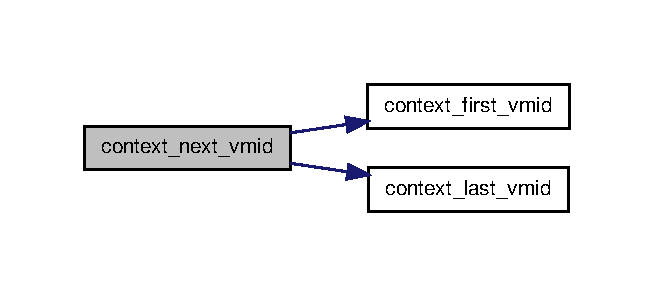
\includegraphics[width=314pt]{context_8c_a5719d5d4a8d98b9784d0f24a2023f05f_cgraph}
\end{center}
\end{figure}


\hypertarget{context_8c_a77fe269a194f9dcfcd0a599a9b6e3bfb}{\index{context.\-c@{context.\-c}!context\-\_\-perform\-\_\-switch@{context\-\_\-perform\-\_\-switch}}
\index{context\-\_\-perform\-\_\-switch@{context\-\_\-perform\-\_\-switch}!context.c@{context.\-c}}
\subsubsection[{context\-\_\-perform\-\_\-switch}]{\setlength{\rightskip}{0pt plus 5cm}{\bf hvmm\-\_\-status\-\_\-t} {\bf context\-\_\-perform\-\_\-switch} (
\begin{DoxyParamCaption}
\item[{void}]{}
\end{DoxyParamCaption}
)}}\label{context_8c_a77fe269a194f9dcfcd0a599a9b6e3bfb}


\-Definition at line 419 of file context.\-c.


\begin{DoxyCode}
{
    hvmm_status_t result = HVMM_STATUS_IGNORED;

    if ( _current_guest_vmid == VMID_INVALID ) {
        printh("context: launching the first guest\n");
        /* very first time, to the default first guest */
        result = context_perform_switch_to_guest_regs( 0, _next_guest_vmid );
        /* DOES NOT COME BACK HERE */
    } else if ( _next_guest_vmid != VMID_INVALID && _current_guest_vmid != 
      _next_guest_vmid ) {
        struct arch_regs *regs = trap_saved_regs();
        if ( (regs->cpsr & 0x1F) != 0x1A ) {
            printh("curr: %x\n", _current_guest_vmid);
            printh("next: %x\n", _next_guest_vmid);

            /* Only if not from Hyp */
            result = context_perform_switch_to_guest_regs( regs, 
      _next_guest_vmid );
            _next_guest_vmid = VMID_INVALID;
        }
    } else {
        /* Staying at the currently active guest. Flush out queued virqs since
       we didn't have a chance to switch the context, where virq flush takes place, 
       this time */
        vgic_flush_virqs(_current_guest_vmid);
    }

    _switch_locked = 0;
    return result;
}
\end{DoxyCode}


\-Here is the call graph for this function\-:
\nopagebreak
\begin{figure}[H]
\begin{center}
\leavevmode
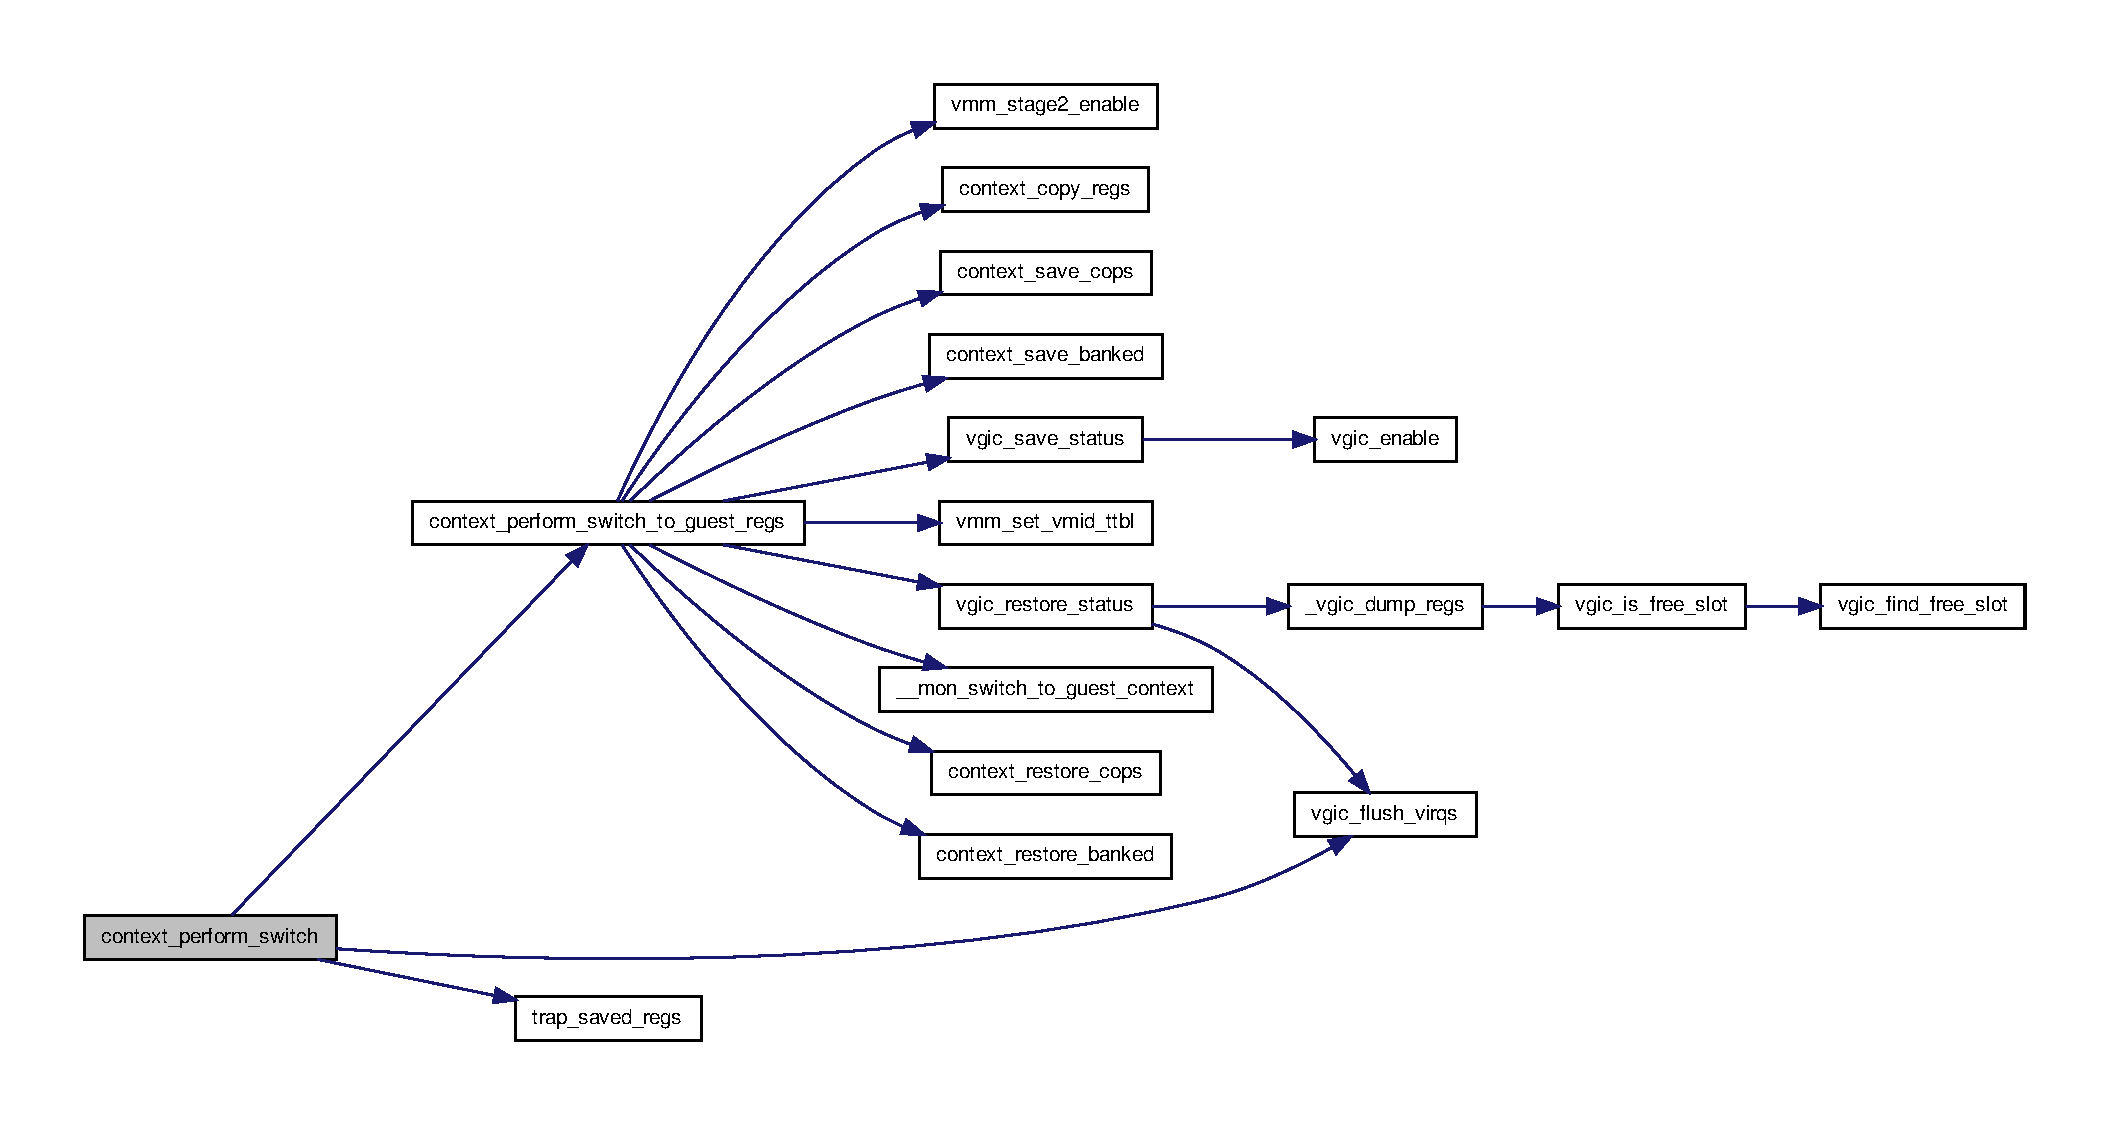
\includegraphics[width=350pt]{context_8c_a77fe269a194f9dcfcd0a599a9b6e3bfb_cgraph}
\end{center}
\end{figure}


\hypertarget{context_8c_adbcfdbfe8d61021879f1622e2c6dc29c}{\index{context.\-c@{context.\-c}!context\-\_\-perform\-\_\-switch\-\_\-to\-\_\-guest\-\_\-regs@{context\-\_\-perform\-\_\-switch\-\_\-to\-\_\-guest\-\_\-regs}}
\index{context\-\_\-perform\-\_\-switch\-\_\-to\-\_\-guest\-\_\-regs@{context\-\_\-perform\-\_\-switch\-\_\-to\-\_\-guest\-\_\-regs}!context.c@{context.\-c}}
\subsubsection[{context\-\_\-perform\-\_\-switch\-\_\-to\-\_\-guest\-\_\-regs}]{\setlength{\rightskip}{0pt plus 5cm}static {\bf hvmm\-\_\-status\-\_\-t} {\bf context\-\_\-perform\-\_\-switch\-\_\-to\-\_\-guest\-\_\-regs} (
\begin{DoxyParamCaption}
\item[{struct {\bf arch\-\_\-regs} $\ast$}]{regs\-\_\-current, }
\item[{{\bf vmid\-\_\-t}}]{next\-\_\-vmid}
\end{DoxyParamCaption}
)\hspace{0.3cm}{\ttfamily  \mbox{[}static\mbox{]}}}}\label{context_8c_adbcfdbfe8d61021879f1622e2c6dc29c}


\-Definition at line 345 of file context.\-c.


\begin{DoxyCode}
{
    /* _curreng_guest_vmid -> next_vmid */

    hvmm_status_t result = HVMM_STATUS_UNKNOWN_ERROR;
    struct hyp_guest_context *context = 0;
    struct arch_regs *regs = 0;
    
    HVMM_TRACE_ENTER();

    if ( _current_guest_vmid == next_vmid ) {
        /* the same guest? WTF? */
        return HVMM_STATUS_IGNORED;
    }

    /*
     * We assume VTCR has been configured and initialized in the memory
       management module
     */
    /* Disable Stage 2 Translation: HCR.VM = 0 */
    vmm_stage2_enable(0);

    if ( regs_current != 0 ) {
        /* save the current guest's context */
        context = &guest_contexts[_current_guest_vmid];
        regs = &context->regs;
        context_copy_regs( regs, regs_current );
        context_save_cops( &context->regs_cop );
        context_save_banked( &context->regs_banked );
        vgic_save_status( &context->vgic_status, context->vmid );
        printh( "context: saving vmid[%d] mode(%x):%s pc:0x%x\n", 
                _current_guest_vmid, 
                regs->cpsr & 0x1F, 
                _modename(regs->cpsr & 0x1F),
                regs->pc
       );
    }

    /* The context of the next guest */
    context = &guest_contexts[next_vmid];

    /* Restore Translation Table for the next guest and Enable Stage 2
       Translation */
    vmm_set_vmid_ttbl( context->vmid, context->ttbl );
    vmm_stage2_enable(1);
    vgic_restore_status( &context->vgic_status, context->vmid );
    
    {
        uint32_t lr = 0;
        asm volatile( "mov  %0, lr" : "=r" (lr) : : "memory", "cc");
        printh( "context: restoring vmid[%d] mode(%x):%s pc:0x%x lr:0x%x\n", 
            next_vmid, 
            context->regs.cpsr & 0x1F, 
            _modename(context->regs.cpsr & 0x1F),
            context->regs.pc, lr
        );
    }

    /* The next becomes the current */
    _current_guest_vmid = next_vmid;
    if ( regs_current == 0 ) {
        /* init -> hyp mode -> guest */
        /* The actual context switching (Hyp to Normal mode) handled in the asm
       code */
        __mon_switch_to_guest_context( &context->regs );
    } else {
        /* guest -> hyp -> guest */
        context_copy_regs( regs_current, &context->regs );
        context_restore_cops( &context->regs_cop );
        context_restore_banked( &context->regs_banked );
    }

    result = HVMM_STATUS_SUCCESS;
    HVMM_TRACE_EXIT();
    return result;
}
\end{DoxyCode}


\-Here is the call graph for this function\-:
\nopagebreak
\begin{figure}[H]
\begin{center}
\leavevmode
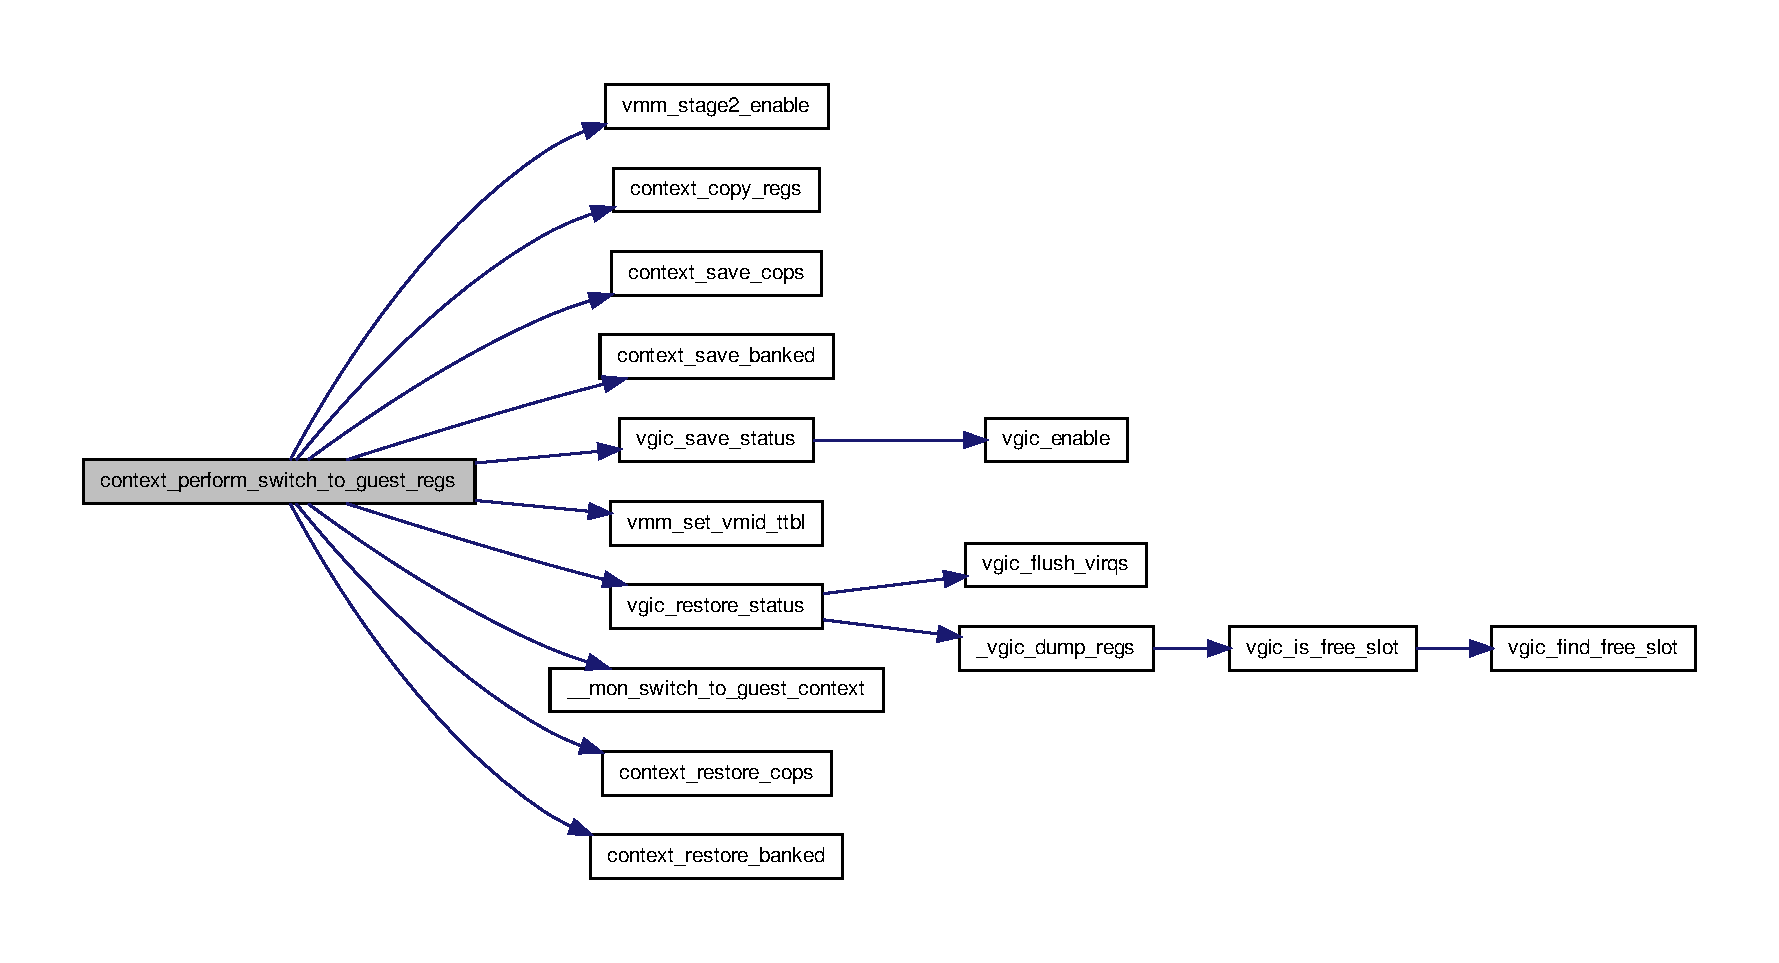
\includegraphics[width=350pt]{context_8c_adbcfdbfe8d61021879f1622e2c6dc29c_cgraph}
\end{center}
\end{figure}


\hypertarget{context_8c_a94bb8d6785586134cc873c061076d323}{\index{context.\-c@{context.\-c}!context\-\_\-restore\-\_\-banked@{context\-\_\-restore\-\_\-banked}}
\index{context\-\_\-restore\-\_\-banked@{context\-\_\-restore\-\_\-banked}!context.c@{context.\-c}}
\subsubsection[{context\-\_\-restore\-\_\-banked}]{\setlength{\rightskip}{0pt plus 5cm}void {\bf context\-\_\-restore\-\_\-banked} (
\begin{DoxyParamCaption}
\item[{struct {\bf arch\-\_\-regs\-\_\-banked} $\ast$}]{regs\-\_\-banked}
\end{DoxyParamCaption}
)}}\label{context_8c_a94bb8d6785586134cc873c061076d323}


\-Definition at line 257 of file context.\-c.


\begin{DoxyCode}
{
    /* USR banked register */
    asm volatile (" msr    sp_usr, %0\n\t"
                          ::"r" (regs_banked->sp_usr) :"memory", "cc");

    /* SVC banked register */
    asm volatile (" msr    spsr_svc, %0\n\t"
                          ::"r" (regs_banked->spsr_svc) :"memory", "cc");
    asm volatile (" msr    sp_svc, %0\n\t"
                          ::"r" (regs_banked->sp_svc) :"memory", "cc");
    asm volatile (" msr    lr_svc, %0\n\t"
                          ::"r" (regs_banked->lr_svc) :"memory", "cc");

    /* ABT banked register */
    asm volatile (" msr    spsr_abt, %0\n\t"
                          ::"r" (regs_banked->spsr_abt) :"memory", "cc");
    asm volatile (" msr    sp_abt, %0\n\t"
                          ::"r" (regs_banked->sp_abt) :"memory", "cc");
    asm volatile (" msr    lr_abt, %0\n\t"
                          ::"r" (regs_banked->lr_abt) :"memory", "cc");

    /* UND banked register */
    asm volatile (" msr    spsr_und, %0\n\t"
                          ::"r" (regs_banked->spsr_und) :"memory", "cc");
    asm volatile (" msr    sp_und, %0\n\t"
                          ::"r" (regs_banked->sp_und) :"memory", "cc");
    asm volatile (" msr    lr_und, %0\n\t"
                          ::"r" (regs_banked->lr_und) :"memory", "cc");

    /* IRQ banked register */
    asm volatile (" msr     spsr_irq, %0\n\t"
                          ::"r" (regs_banked->spsr_irq) :"memory", "cc");
    asm volatile (" msr     sp_irq, %0\n\t"
                          ::"r" (regs_banked->sp_irq) :"memory", "cc");
    asm volatile (" msr     lr_irq, %0\n\t"
                          ::"r" (regs_banked->lr_irq) :"memory", "cc");

    /* FIQ banked register */
    asm volatile (" msr     spsr_fiq, %0\n\t"
                          ::"r" (regs_banked->spsr_fiq) :"memory", "cc");
    asm volatile (" msr     lr_fiq, %0\n\t"
                          ::"r" (regs_banked->lr_fiq) :"memory", "cc");
    asm volatile (" msr    r8_fiq, %0\n\t"
                          ::"r" (regs_banked->r8_fiq) :"memory", "cc");
    asm volatile (" msr    r9_fiq, %0\n\t"
                          ::"r" (regs_banked->r9_fiq) :"memory", "cc");
    asm volatile (" msr    r10_fiq, %0\n\t"
                          ::"r" (regs_banked->r10_fiq) :"memory", "cc");
    asm volatile (" msr    r11_fiq, %0\n\t"
                          ::"r" (regs_banked->r11_fiq) :"memory", "cc");
    asm volatile (" msr    r12_fiq, %0\n\t"
                          ::"r" (regs_banked->r12_fiq) :"memory", "cc");
}
\end{DoxyCode}
\hypertarget{context_8c_a2d3fdf44ea523c8f4978cf9c33107768}{\index{context.\-c@{context.\-c}!context\-\_\-restore\-\_\-cops@{context\-\_\-restore\-\_\-cops}}
\index{context\-\_\-restore\-\_\-cops@{context\-\_\-restore\-\_\-cops}!context.c@{context.\-c}}
\subsubsection[{context\-\_\-restore\-\_\-cops}]{\setlength{\rightskip}{0pt plus 5cm}void {\bf context\-\_\-restore\-\_\-cops} (
\begin{DoxyParamCaption}
\item[{struct {\bf arch\-\_\-regs\-\_\-cop} $\ast$}]{regs\-\_\-cop}
\end{DoxyParamCaption}
)}}\label{context_8c_a2d3fdf44ea523c8f4978cf9c33107768}


\-Definition at line 331 of file context.\-c.


\begin{DoxyCode}
{
    write_vbar(regs_cop->vbar);
    write_ttbr0(regs_cop->ttbr0);
    write_ttbr1(regs_cop->ttbr1);
    write_ttbcr(regs_cop->ttbcr);
    write_sctlr(regs_cop->sctlr);
}
\end{DoxyCode}
\hypertarget{context_8c_a57af844ae7e83a33d88a4c36eee930eb}{\index{context.\-c@{context.\-c}!context\-\_\-save\-\_\-banked@{context\-\_\-save\-\_\-banked}}
\index{context\-\_\-save\-\_\-banked@{context\-\_\-save\-\_\-banked}!context.c@{context.\-c}}
\subsubsection[{context\-\_\-save\-\_\-banked}]{\setlength{\rightskip}{0pt plus 5cm}void {\bf context\-\_\-save\-\_\-banked} (
\begin{DoxyParamCaption}
\item[{struct {\bf arch\-\_\-regs\-\_\-banked} $\ast$}]{regs\-\_\-banked}
\end{DoxyParamCaption}
)}}\label{context_8c_a57af844ae7e83a33d88a4c36eee930eb}


\-Definition at line 201 of file context.\-c.


\begin{DoxyCode}
{
    /* USR banked register */
    asm volatile (" mrs     %0, sp_usr\n\t"
                          :"=r" (regs_banked->sp_usr)::"memory", "cc");

    /* SVC banked register */
    asm volatile (" mrs     %0, spsr_svc\n\t"
                          :"=r" (regs_banked->spsr_svc)::"memory", "cc");
    asm volatile (" mrs     %0, sp_svc\n\t"
                          :"=r" (regs_banked->sp_svc)::"memory", "cc");
    asm volatile (" mrs     %0, lr_svc\n\t"
                          :"=r" (regs_banked->lr_svc)::"memory", "cc");

    /* ABT banked register */
    asm volatile (" mrs     %0, spsr_abt\n\t"
                          :"=r" (regs_banked->spsr_abt)::"memory", "cc");
    asm volatile (" mrs     %0, sp_abt\n\t"
                          :"=r" (regs_banked->sp_abt)::"memory", "cc");
    asm volatile (" mrs     %0, lr_abt\n\t"
                          :"=r" (regs_banked->lr_abt)::"memory", "cc");

    /* UND banked register */
    asm volatile (" mrs     %0, spsr_und\n\t"
                          :"=r" (regs_banked->spsr_und)::"memory", "cc");
    asm volatile (" mrs     %0, sp_und\n\t"
                          :"=r" (regs_banked->sp_und)::"memory", "cc");
    asm volatile (" mrs     %0, lr_und\n\t"
                          :"=r" (regs_banked->lr_und)::"memory", "cc");

    /* IRQ banked register */
    asm volatile (" mrs     %0, spsr_irq\n\t"
                          :"=r" (regs_banked->spsr_irq)::"memory", "cc");
    asm volatile (" mrs     %0, sp_irq\n\t"
                          :"=r" (regs_banked->sp_irq)::"memory", "cc");
    asm volatile (" mrs     %0, lr_irq\n\t"
                          :"=r" (regs_banked->lr_irq)::"memory", "cc");

    /* FIQ banked register  R8_fiq ~ R12_fiq, LR and SPSR */
    asm volatile (" mrs     %0, spsr_fiq\n\t"
                          :"=r" (regs_banked->spsr_fiq)::"memory", "cc");
    asm volatile (" mrs     %0, lr_fiq\n\t"
                          :"=r" (regs_banked->lr_fiq)::"memory", "cc");
    asm volatile (" mrs     %0, r8_fiq\n\t"
                          :"=r" (regs_banked->r8_fiq)::"memory", "cc");
    asm volatile (" mrs     %0, r9_fiq\n\t"
                          :"=r" (regs_banked->r9_fiq)::"memory", "cc");
    asm volatile (" mrs     %0, r10_fiq\n\t"
                          :"=r" (regs_banked->r10_fiq)::"memory", "cc");
    asm volatile (" mrs     %0, r11_fiq\n\t"
                          :"=r" (regs_banked->r11_fiq)::"memory", "cc");
    asm volatile (" mrs     %0, r12_fiq\n\t"
                          :"=r" (regs_banked->r12_fiq)::"memory", "cc");

}
\end{DoxyCode}
\hypertarget{context_8c_a9a5bddd4742fe9c4cc8ee9fa50cf03bf}{\index{context.\-c@{context.\-c}!context\-\_\-save\-\_\-cops@{context\-\_\-save\-\_\-cops}}
\index{context\-\_\-save\-\_\-cops@{context\-\_\-save\-\_\-cops}!context.c@{context.\-c}}
\subsubsection[{context\-\_\-save\-\_\-cops}]{\setlength{\rightskip}{0pt plus 5cm}void {\bf context\-\_\-save\-\_\-cops} (
\begin{DoxyParamCaption}
\item[{struct {\bf arch\-\_\-regs\-\_\-cop} $\ast$}]{regs\-\_\-cop}
\end{DoxyParamCaption}
)}}\label{context_8c_a9a5bddd4742fe9c4cc8ee9fa50cf03bf}


\-Definition at line 322 of file context.\-c.


\begin{DoxyCode}
{
    regs_cop->vbar = read_vbar();
    regs_cop->ttbr0 = read_ttbr0();
    regs_cop->ttbr1 = read_ttbr1();
    regs_cop->ttbcr = read_ttbcr();
    regs_cop->sctlr = read_sctlr();
}
\end{DoxyCode}
\hypertarget{context_8c_a39db644c82cc9c99ef78feb58d57b58c}{\index{context.\-c@{context.\-c}!context\-\_\-switch\-\_\-to\-\_\-initial\-\_\-guest@{context\-\_\-switch\-\_\-to\-\_\-initial\-\_\-guest}}
\index{context\-\_\-switch\-\_\-to\-\_\-initial\-\_\-guest@{context\-\_\-switch\-\_\-to\-\_\-initial\-\_\-guest}!context.c@{context.\-c}}
\subsubsection[{context\-\_\-switch\-\_\-to\-\_\-initial\-\_\-guest}]{\setlength{\rightskip}{0pt plus 5cm}void {\bf context\-\_\-switch\-\_\-to\-\_\-initial\-\_\-guest} (
\begin{DoxyParamCaption}
\item[{void}]{}
\end{DoxyParamCaption}
)}}\label{context_8c_a39db644c82cc9c99ef78feb58d57b58c}


\-Definition at line 447 of file context.\-c.


\begin{DoxyCode}
{
    struct hyp_guest_context *context = 0;
    struct arch_regs *regs = 0;

    uart_print("[hyp] switch_to_initial_guest:\n\r");

    /* Select the first guest context to switch to. */
    _current_guest_vmid = VMID_INVALID;
    context = &guest_contexts[0];

    /* Dump the initial register values of the guest for debugging purpose */
    regs = &context->regs;
    context_dump_regs( regs );

    /* Context Switch with current context == none */
    context_switchto(0);
    context_perform_switch();
}
\end{DoxyCode}


\-Here is the call graph for this function\-:
\nopagebreak
\begin{figure}[H]
\begin{center}
\leavevmode
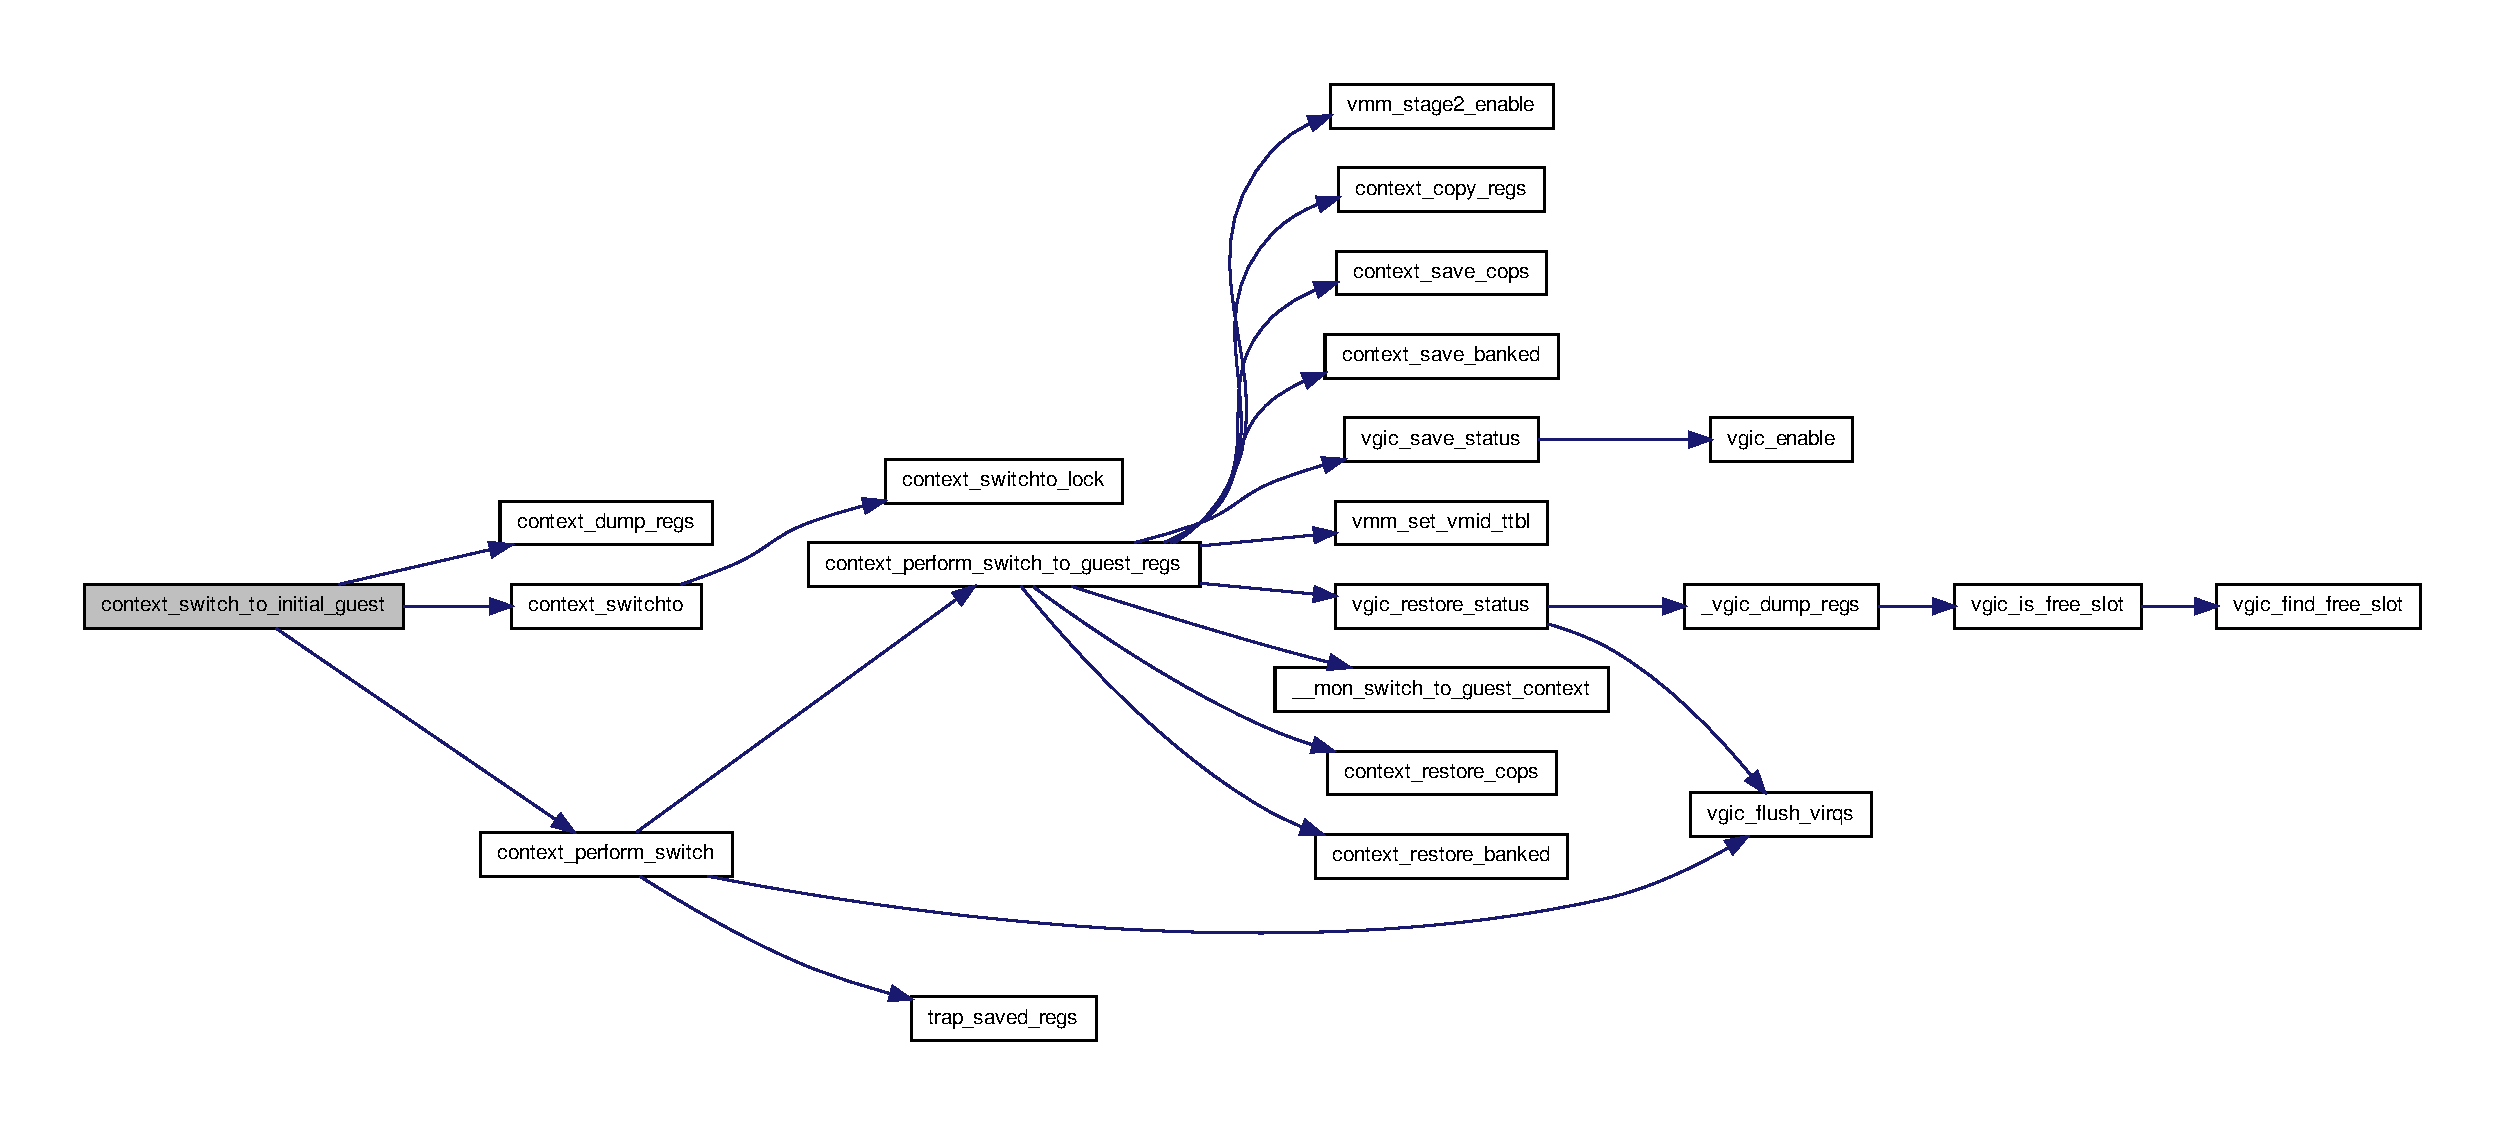
\includegraphics[width=350pt]{context_8c_a39db644c82cc9c99ef78feb58d57b58c_cgraph}
\end{center}
\end{figure}


\hypertarget{context_8c_aaa75f8a973764763b44ca823e02f4406}{\index{context.\-c@{context.\-c}!context\-\_\-switchto@{context\-\_\-switchto}}
\index{context\-\_\-switchto@{context\-\_\-switchto}!context.c@{context.\-c}}
\subsubsection[{context\-\_\-switchto}]{\setlength{\rightskip}{0pt plus 5cm}{\bf hvmm\-\_\-status\-\_\-t} {\bf context\-\_\-switchto} (
\begin{DoxyParamCaption}
\item[{{\bf vmid\-\_\-t}}]{vmid}
\end{DoxyParamCaption}
)}}\label{context_8c_aaa75f8a973764763b44ca823e02f4406}


\-Definition at line 572 of file context.\-c.


\begin{DoxyCode}
{
    return context_switchto_lock(vmid, 0);
}
\end{DoxyCode}


\-Here is the call graph for this function\-:
\nopagebreak
\begin{figure}[H]
\begin{center}
\leavevmode
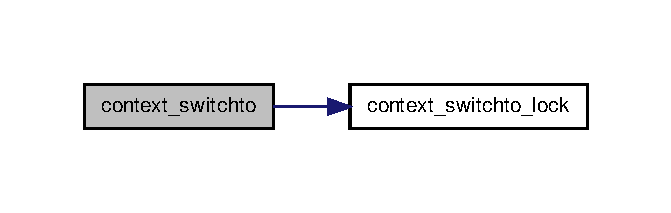
\includegraphics[width=322pt]{context_8c_aaa75f8a973764763b44ca823e02f4406_cgraph}
\end{center}
\end{figure}


\hypertarget{context_8c_a00b56df45d0ef16d93040b667bb025ef}{\index{context.\-c@{context.\-c}!context\-\_\-switchto\-\_\-lock@{context\-\_\-switchto\-\_\-lock}}
\index{context\-\_\-switchto\-\_\-lock@{context\-\_\-switchto\-\_\-lock}!context.c@{context.\-c}}
\subsubsection[{context\-\_\-switchto\-\_\-lock}]{\setlength{\rightskip}{0pt plus 5cm}{\bf hvmm\-\_\-status\-\_\-t} {\bf context\-\_\-switchto\-\_\-lock} (
\begin{DoxyParamCaption}
\item[{{\bf vmid\-\_\-t}}]{vmid, }
\item[{{\bf uint8\-\_\-t}}]{locked}
\end{DoxyParamCaption}
)}}\label{context_8c_a00b56df45d0ef16d93040b667bb025ef}


\-Definition at line 577 of file context.\-c.


\begin{DoxyCode}
{
    hvmm_status_t result = HVMM_STATUS_IGNORED;

    HVMM_TRACE_ENTER();

    /* valid and not current vmid, switch */
    if (_switch_locked == 0) {
        if ( !_valid_vmid(vmid) ) {
            result = HVMM_STATUS_BAD_ACCESS;
        } else {
            _next_guest_vmid = vmid;
            result = HVMM_STATUS_SUCCESS;

            printh("switching to vmid: %x\n", (uint32_t)vmid);
        }
    } else {
        printh("context: next vmid locked to %d\n", _next_guest_vmid );
    }

    if ( locked )
        _switch_locked = locked;

    HVMM_TRACE_EXIT();
    return result;
}
\end{DoxyCode}
\hypertarget{context_8c_a3fd5aa68bf14823442fcc5fda4cb6a51}{\index{context.\-c@{context.\-c}!context\-\_\-waiting\-\_\-vmid@{context\-\_\-waiting\-\_\-vmid}}
\index{context\-\_\-waiting\-\_\-vmid@{context\-\_\-waiting\-\_\-vmid}!context.c@{context.\-c}}
\subsubsection[{context\-\_\-waiting\-\_\-vmid}]{\setlength{\rightskip}{0pt plus 5cm}{\bf vmid\-\_\-t} {\bf context\-\_\-waiting\-\_\-vmid} (
\begin{DoxyParamCaption}
\item[{void}]{}
\end{DoxyParamCaption}
)}}\label{context_8c_a3fd5aa68bf14823442fcc5fda4cb6a51}


\-Definition at line 567 of file context.\-c.


\begin{DoxyCode}
{
    return _next_guest_vmid;
}
\end{DoxyCode}
\hypertarget{context_8c_a83895de158b7efc9456e7475528e42d4}{\index{context.\-c@{context.\-c}!start\-\_\-guest\-\_\-os@{start\-\_\-guest\-\_\-os}}
\index{start\-\_\-guest\-\_\-os@{start\-\_\-guest\-\_\-os}!context.c@{context.\-c}}
\subsubsection[{start\-\_\-guest\-\_\-os}]{\setlength{\rightskip}{0pt plus 5cm}void {\bf start\-\_\-guest\-\_\-os} (
\begin{DoxyParamCaption}
\item[{void}]{}
\end{DoxyParamCaption}
)}}\label{context_8c_a83895de158b7efc9456e7475528e42d4}


\-Definition at line 604 of file context.\-c.


\begin{DoxyCode}
{
    init_print();

    hvmm_status_t ret = HVMM_STATUS_UNKNOWN_ERROR;
    printh("[%s : %d] Starting...\n", __FUNCTION__, __LINE__);

    /* Initialize Memory Management */
    ret = hvmm_mm_init();

    /* Initialize Interrupt Management */
    ret = hvmm_interrupt_init();
    if ( ret != HVMM_STATUS_SUCCESS ) {
        uart_print("[hyp_main] interrupt initialization failed...\n\r");
    }

    /* Initialize Guests */
    context_init_guests();

    /* Initialize Virtual Devices */
    vdev_init();

    /* Virtual GIC Distributor */
    printh( "tests: Registering sample vdev:'vgicd' at %x\n", CFG_GIC_BASE_PA |
       GIC_OFFSET_GICD);
    vdev_gicd_init(CFG_GIC_BASE_PA | GIC_OFFSET_GICD);

    /* Initialize PIRQ to VIRQ mapping */
    virqmap_init();

    /* Start Scheduling */
    scheduler_test_scheduling();

    /* Begin running test code for newly implemented features */
    hvmm_tests_main();

    /* Print Banner */
    printH("%s", BANNER_STRING);

    /* Switch to the first guest */
    context_switch_to_initial_guest();

    /* The code flow must not reach here */
    uart_print("[hyp_main] ERROR: CODE MUST NOT REACH HERE\n\r");
    hyp_abort_infinite();
}
\end{DoxyCode}


\-Here is the call graph for this function\-:
\nopagebreak
\begin{figure}[H]
\begin{center}
\leavevmode
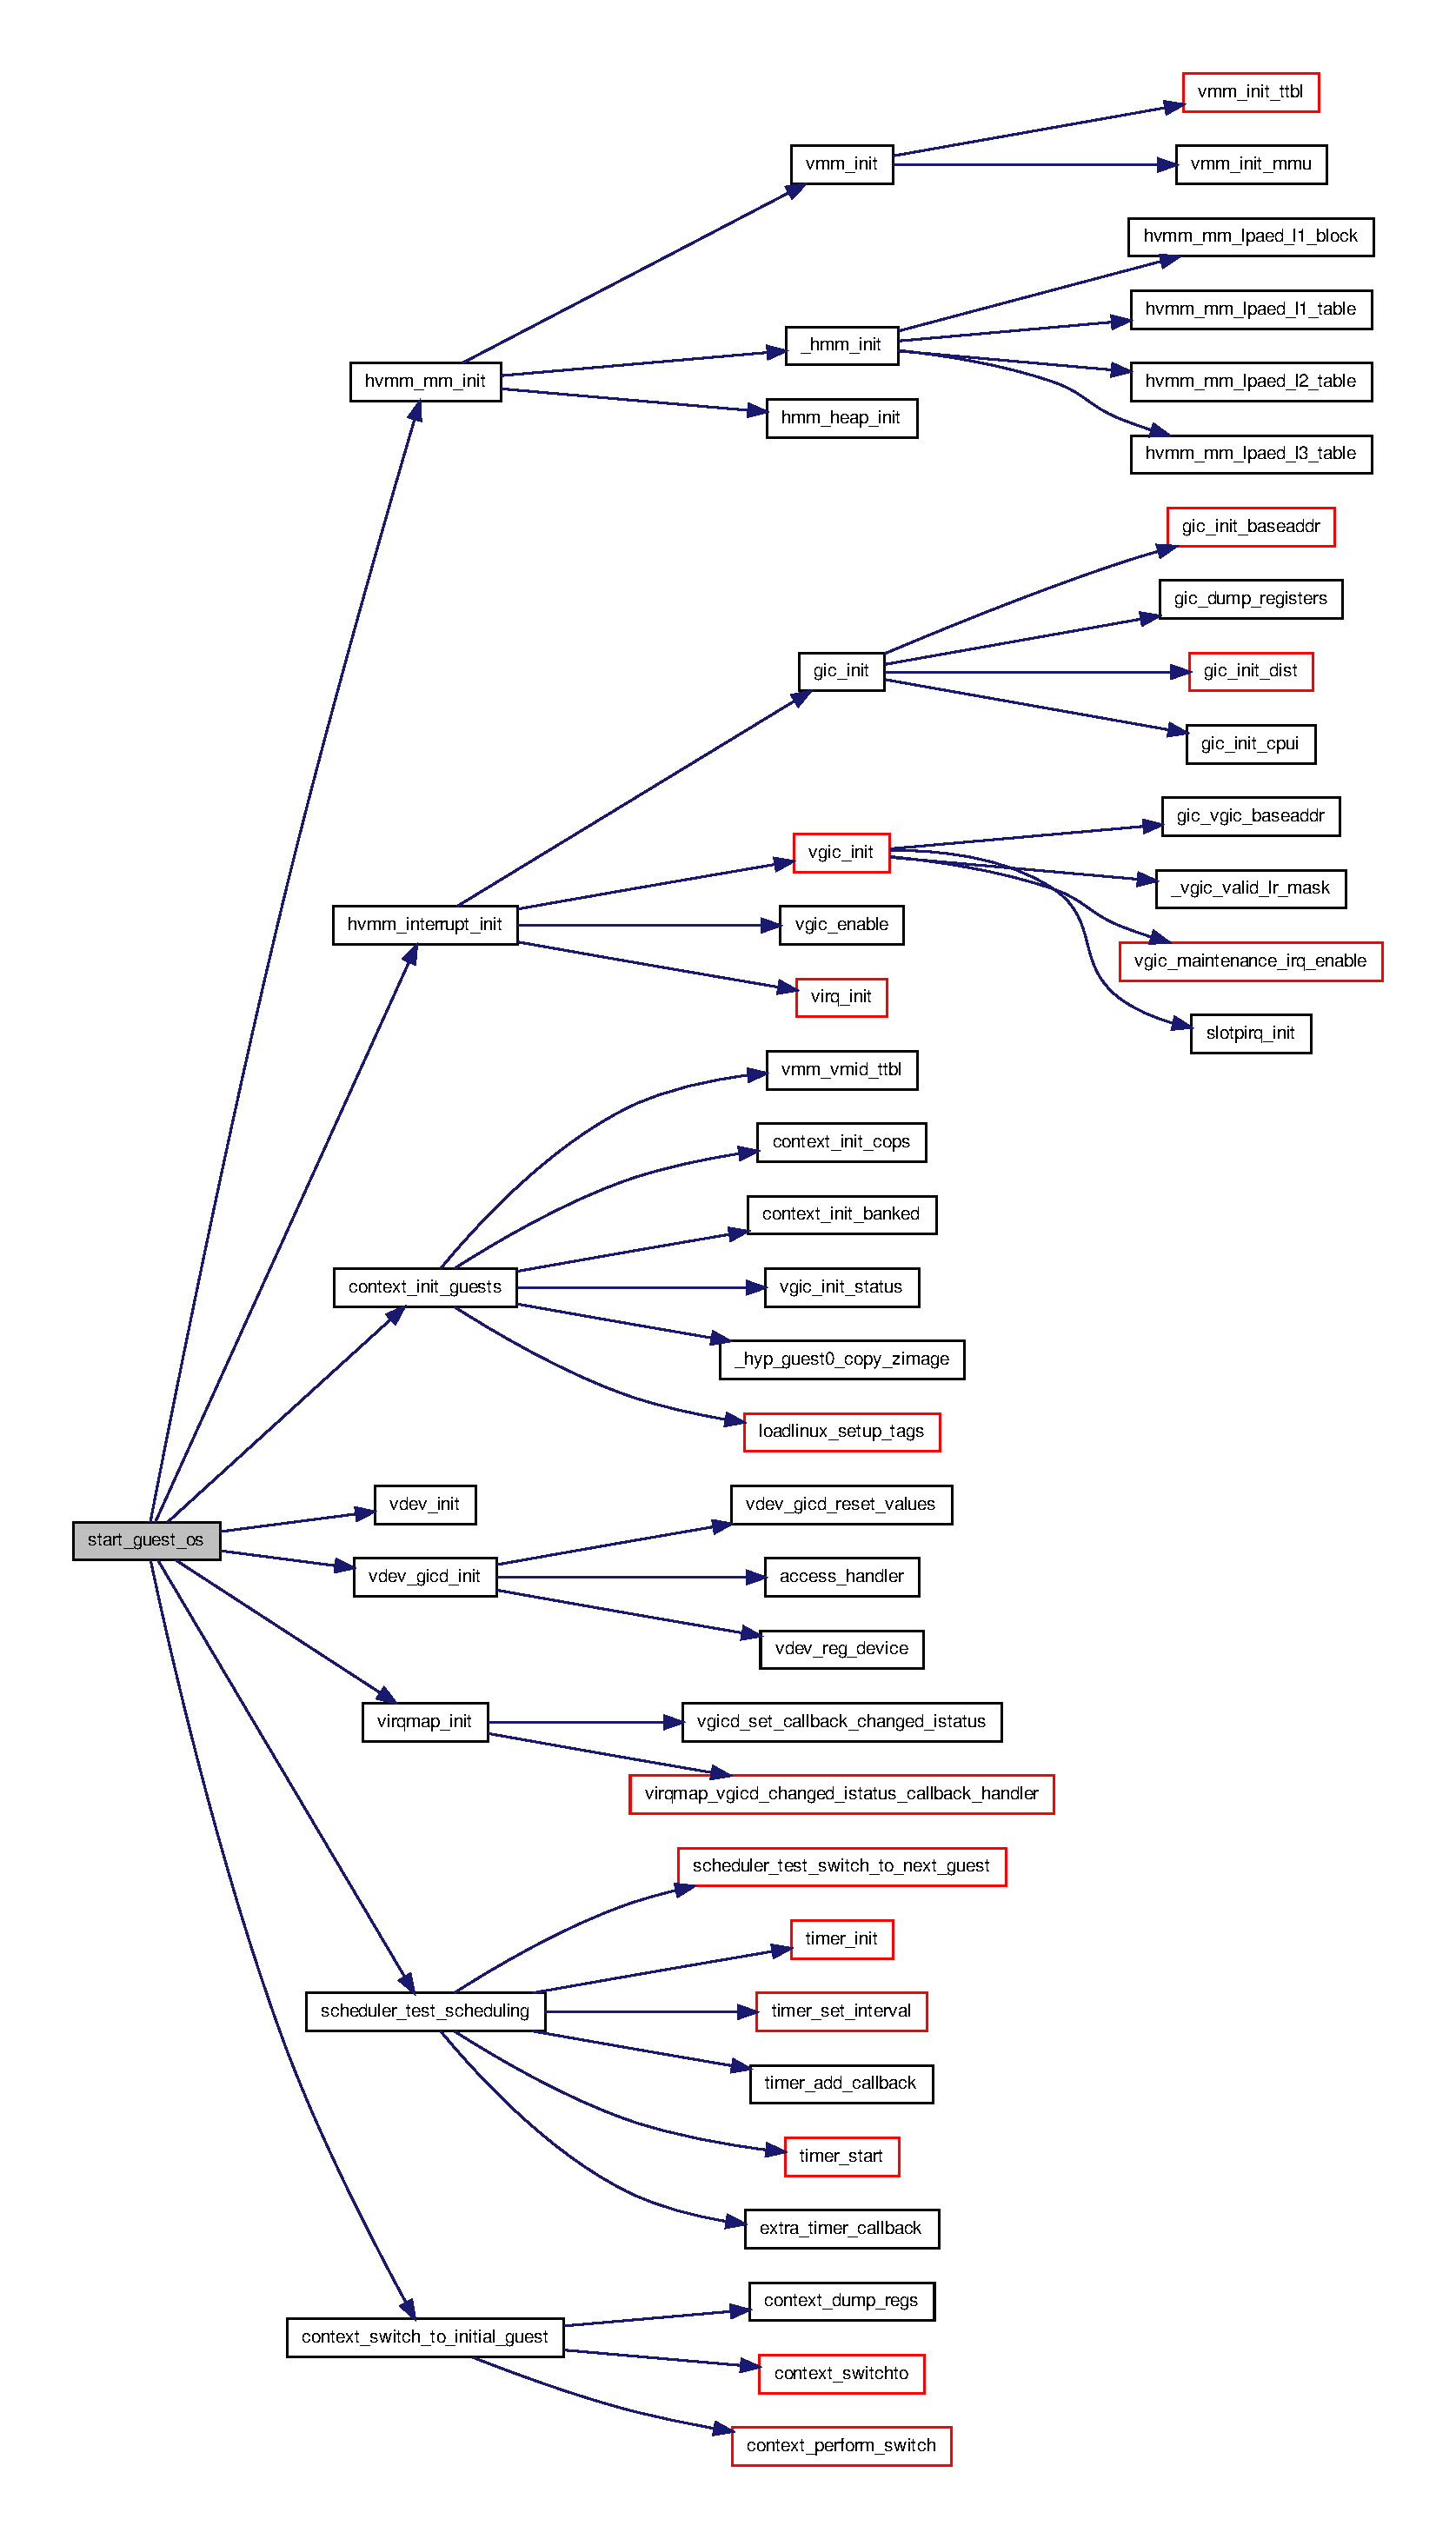
\includegraphics[height=550pt]{context_8c_a83895de158b7efc9456e7475528e42d4_cgraph}
\end{center}
\end{figure}




\subsection{\-Variable \-Documentation}
\hypertarget{context_8c_a5de72a0d4dd972c7d7d8c9d08272d9e8}{\index{context.\-c@{context.\-c}!\-\_\-current\-\_\-guest\-\_\-vmid@{\-\_\-current\-\_\-guest\-\_\-vmid}}
\index{\-\_\-current\-\_\-guest\-\_\-vmid@{\-\_\-current\-\_\-guest\-\_\-vmid}!context.c@{context.\-c}}
\subsubsection[{\-\_\-current\-\_\-guest\-\_\-vmid}]{\setlength{\rightskip}{0pt plus 5cm}int {\bf \-\_\-current\-\_\-guest\-\_\-vmid} = {\bf \-V\-M\-I\-D\-\_\-\-I\-N\-V\-A\-L\-I\-D}\hspace{0.3cm}{\ttfamily  \mbox{[}static\mbox{]}}}}\label{context_8c_a5de72a0d4dd972c7d7d8c9d08272d9e8}


\-Definition at line 50 of file context.\-c.

\hypertarget{context_8c_a5f1b0bb9a3d788646bb83d32d12419f3}{\index{context.\-c@{context.\-c}!\-\_\-next\-\_\-guest\-\_\-vmid@{\-\_\-next\-\_\-guest\-\_\-vmid}}
\index{\-\_\-next\-\_\-guest\-\_\-vmid@{\-\_\-next\-\_\-guest\-\_\-vmid}!context.c@{context.\-c}}
\subsubsection[{\-\_\-next\-\_\-guest\-\_\-vmid}]{\setlength{\rightskip}{0pt plus 5cm}int {\bf \-\_\-next\-\_\-guest\-\_\-vmid} = {\bf \-V\-M\-I\-D\-\_\-\-I\-N\-V\-A\-L\-I\-D}\hspace{0.3cm}{\ttfamily  \mbox{[}static\mbox{]}}}}\label{context_8c_a5f1b0bb9a3d788646bb83d32d12419f3}


\-Definition at line 51 of file context.\-c.

\hypertarget{context_8c_a345440f03deca2090efe13b08eaead89}{\index{context.\-c@{context.\-c}!\-\_\-switch\-\_\-locked@{\-\_\-switch\-\_\-locked}}
\index{\-\_\-switch\-\_\-locked@{\-\_\-switch\-\_\-locked}!context.c@{context.\-c}}
\subsubsection[{\-\_\-switch\-\_\-locked}]{\setlength{\rightskip}{0pt plus 5cm}{\bf uint8\-\_\-t} {\bf \-\_\-switch\-\_\-locked} = 0\hspace{0.3cm}{\ttfamily  \mbox{[}static\mbox{]}}}}\label{context_8c_a345440f03deca2090efe13b08eaead89}


\-Definition at line 52 of file context.\-c.

\hypertarget{context_8c_a7a55b222a2790b315eaf5dbe7a12c407}{\index{context.\-c@{context.\-c}!guest\-\_\-contexts@{guest\-\_\-contexts}}
\index{guest\-\_\-contexts@{guest\-\_\-contexts}!context.c@{context.\-c}}
\subsubsection[{guest\-\_\-contexts}]{\setlength{\rightskip}{0pt plus 5cm}struct {\bf hyp\-\_\-guest\-\_\-context} {\bf guest\-\_\-contexts}\mbox{[}{\bf \-N\-U\-M\-\_\-\-G\-U\-E\-S\-T\-\_\-\-C\-O\-N\-T\-E\-X\-T\-S}\mbox{]}\hspace{0.3cm}{\ttfamily  \mbox{[}static\mbox{]}}}}\label{context_8c_a7a55b222a2790b315eaf5dbe7a12c407}


\-Definition at line 49 of file context.\-c.


\hypertarget{context_8h}{\section{context.\-h \-File \-Reference}
\label{context_8h}\index{context.\-h@{context.\-h}}
}
{\ttfamily \#include $<$k-\/hypervisor-\/config.\-h$>$}\*
{\ttfamily \#include \char`\"{}arch\-\_\-types.\-h\char`\"{}}\*
{\ttfamily \#include \char`\"{}vgic.\-h\char`\"{}}\*
{\ttfamily \#include \char`\"{}lpae.\-h\char`\"{}}\*
\-Include dependency graph for context.\-h\-:
\nopagebreak
\begin{figure}[H]
\begin{center}
\leavevmode
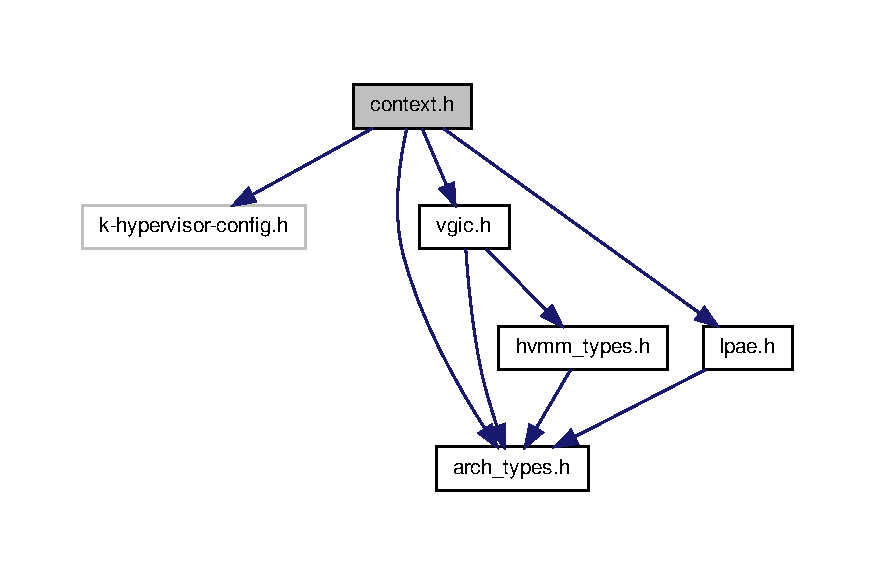
\includegraphics[width=350pt]{context_8h__incl}
\end{center}
\end{figure}
\-This graph shows which files directly or indirectly include this file\-:
\nopagebreak
\begin{figure}[H]
\begin{center}
\leavevmode
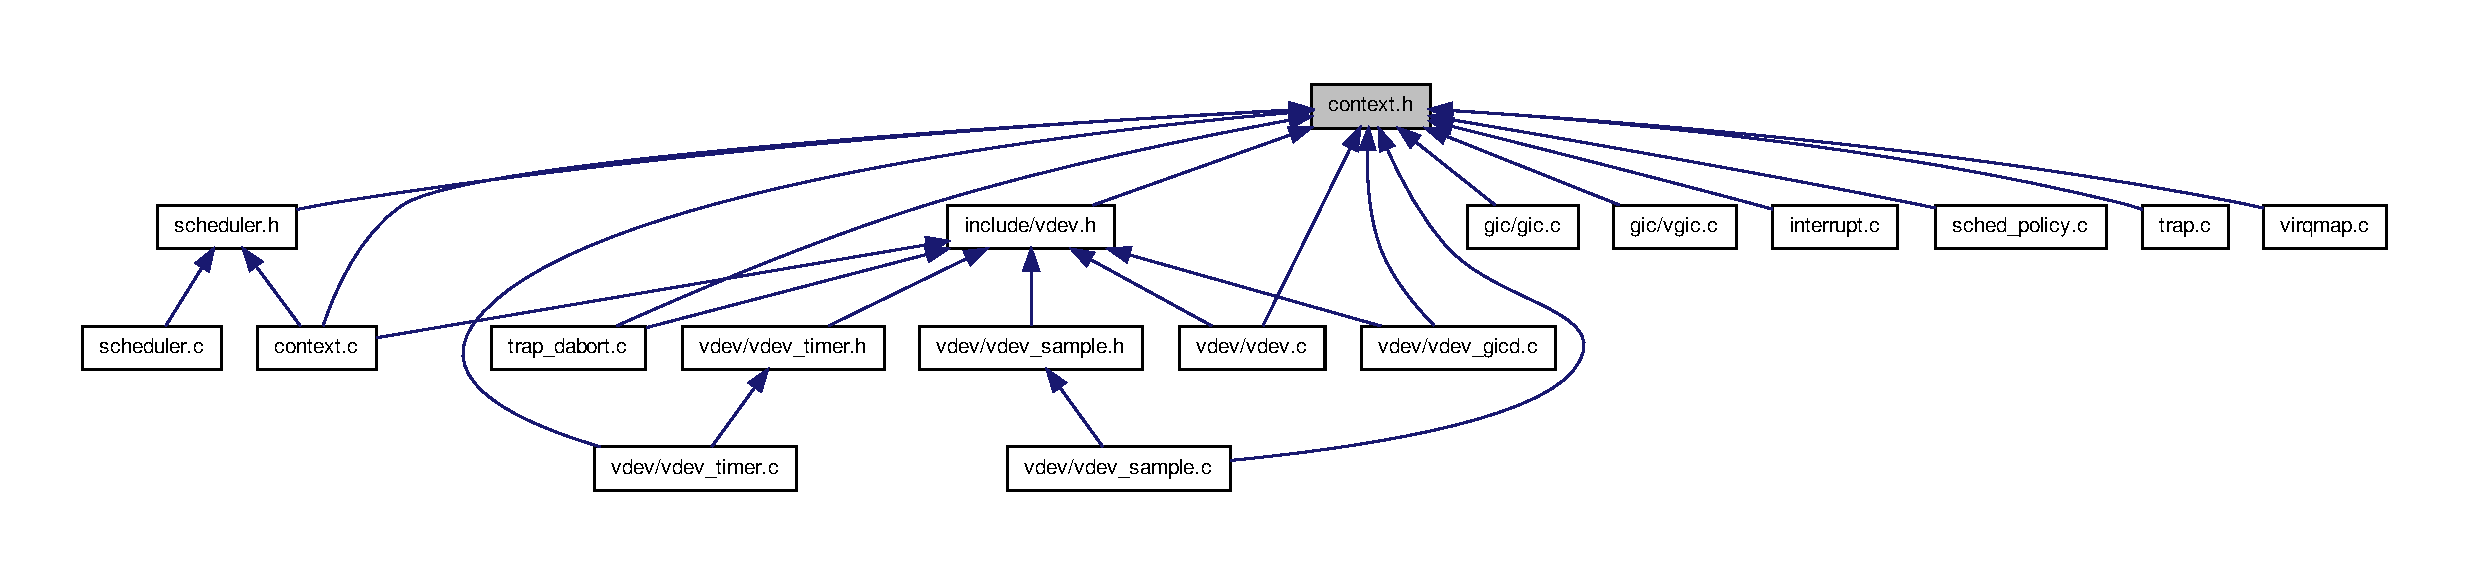
\includegraphics[width=350pt]{context_8h__dep__incl}
\end{center}
\end{figure}
\subsection*{\-Data \-Structures}
\begin{DoxyCompactItemize}
\item 
struct \hyperlink{structarch__regs}{arch\-\_\-regs}
\item 
struct \hyperlink{structarch__regs__cop}{arch\-\_\-regs\-\_\-cop}
\item 
struct \hyperlink{structarch__regs__banked}{arch\-\_\-regs\-\_\-banked}
\item 
struct \hyperlink{structhyp__guest__context}{hyp\-\_\-guest\-\_\-context}
\end{DoxyCompactItemize}
\subsection*{\-Defines}
\begin{DoxyCompactItemize}
\item 
\#define \hyperlink{context_8h_a469821668f7cfd63c2dd4f05120f1ccf}{\-A\-R\-C\-H\-\_\-\-R\-E\-G\-S\-\_\-\-N\-U\-M\-\_\-\-G\-P\-R}~13
\end{DoxyCompactItemize}
\subsection*{\-Enumerations}
\begin{DoxyCompactItemize}
\item 
enum \hyperlink{context_8h_a5588893c974f2fb0f974e18a49110488}{hyp\-\_\-hvc\-\_\-result\-\_\-t} \{ \hyperlink{context_8h_a5588893c974f2fb0f974e18a49110488ac5463bbf590e31d3f3d2bf1e6ae1bd39}{\-H\-Y\-P\-\_\-\-R\-E\-S\-U\-L\-T\-\_\-\-E\-R\-E\-T} =  0, 
\hyperlink{context_8h_a5588893c974f2fb0f974e18a49110488a5307b6644c0db1e03ef3025951f8a8b4}{\-H\-Y\-P\-\_\-\-R\-E\-S\-U\-L\-T\-\_\-\-S\-T\-A\-Y} =  1
 \}
\end{DoxyCompactItemize}
\subsection*{\-Functions}
\begin{DoxyCompactItemize}
\item 
struct \hyperlink{structarch__regs}{arch\-\_\-regs} \hyperlink{context_8h_a81c6ca411c5d54e1c6c30c0142e7a8df}{\-\_\-\-\_\-attribute} ((packed))
\item 
void \hyperlink{context_8h_aa662295d6861cedca861f13c4ad5ece4}{context\-\_\-dump\-\_\-regs} (struct \hyperlink{structarch__regs}{arch\-\_\-regs} $\ast$\hyperlink{vdev__timer_8c_a514d7f36beee4b3e39da305e12d39d0a}{regs})
\item 
void \hyperlink{context_8h_a39db644c82cc9c99ef78feb58d57b58c}{context\-\_\-switch\-\_\-to\-\_\-initial\-\_\-guest} (void)
\item 
void \hyperlink{context_8h_a0abdd106a2b654464230b622b4c9877e}{context\-\_\-init\-\_\-guests} (void)
\item 
\hyperlink{hvmm__types_8h_a39d593b2c97852f566d7472b76ab7ba2}{hvmm\-\_\-status\-\_\-t} \hyperlink{context_8h_a77fe269a194f9dcfcd0a599a9b6e3bfb}{context\-\_\-perform\-\_\-switch} (void)
\item 
\hyperlink{hvmm__types_8h_af7e9bd0adfb7d10e7a7a0ee60a5f962c}{vmid\-\_\-t} \hyperlink{context_8h_a525fcf860b6f33b4192443c9d66ba4f6}{context\-\_\-current\-\_\-vmid} (void)
\item 
\hyperlink{hvmm__types_8h_af7e9bd0adfb7d10e7a7a0ee60a5f962c}{vmid\-\_\-t} \hyperlink{context_8h_a3fd5aa68bf14823442fcc5fda4cb6a51}{context\-\_\-waiting\-\_\-vmid} (void)
\item 
\hyperlink{hvmm__types_8h_a39d593b2c97852f566d7472b76ab7ba2}{hvmm\-\_\-status\-\_\-t} \hyperlink{context_8h_aaa75f8a973764763b44ca823e02f4406}{context\-\_\-switchto} (\hyperlink{hvmm__types_8h_af7e9bd0adfb7d10e7a7a0ee60a5f962c}{vmid\-\_\-t} vmid)
\item 
\hyperlink{hvmm__types_8h_a39d593b2c97852f566d7472b76ab7ba2}{hvmm\-\_\-status\-\_\-t} \hyperlink{context_8h_a00b56df45d0ef16d93040b667bb025ef}{context\-\_\-switchto\-\_\-lock} (\hyperlink{hvmm__types_8h_af7e9bd0adfb7d10e7a7a0ee60a5f962c}{vmid\-\_\-t} vmid, \hyperlink{arch__types_8h_aba7bc1797add20fe3efdf37ced1182c5}{uint8\-\_\-t} locked)
\item 
\hyperlink{hvmm__types_8h_af7e9bd0adfb7d10e7a7a0ee60a5f962c}{vmid\-\_\-t} \hyperlink{context_8h_a891f8f7028b04322da205990de1a8f5b}{context\-\_\-first\-\_\-vmid} (void)
\item 
\hyperlink{hvmm__types_8h_af7e9bd0adfb7d10e7a7a0ee60a5f962c}{vmid\-\_\-t} \hyperlink{context_8h_ad48a9977fdb537cc020b451e08dfc590}{context\-\_\-last\-\_\-vmid} (void)
\item 
\hyperlink{hvmm__types_8h_af7e9bd0adfb7d10e7a7a0ee60a5f962c}{vmid\-\_\-t} \hyperlink{context_8h_a5719d5d4a8d98b9784d0f24a2023f05f}{context\-\_\-next\-\_\-vmid} (\hyperlink{hvmm__types_8h_af7e9bd0adfb7d10e7a7a0ee60a5f962c}{vmid\-\_\-t} ofvmid)
\item 
struct \hyperlink{structhyp__guest__context}{hyp\-\_\-guest\-\_\-context} $\ast$ \hyperlink{context_8h_ae8e692844cf2c76f7661088f7a7be817}{context\-\_\-atvmid} (\hyperlink{hvmm__types_8h_af7e9bd0adfb7d10e7a7a0ee60a5f962c}{vmid\-\_\-t} vmid)
\item 
void \hyperlink{context_8h_a83895de158b7efc9456e7475528e42d4}{start\-\_\-guest\-\_\-os} (void)
\end{DoxyCompactItemize}
\subsection*{\-Variables}
\begin{DoxyCompactItemize}
\item 
\hyperlink{arch__types_8h_a435d1572bf3f880d55459d9805097f62}{uint32\-\_\-t} \hyperlink{context_8h_a0d1814f5edf1360a76b54ac386be5e85}{cpsr}
\item 
\hyperlink{arch__types_8h_a435d1572bf3f880d55459d9805097f62}{uint32\-\_\-t} \hyperlink{context_8h_a27468faba76ab3fb5458fb06c0f2af8a}{pc}
\item 
\hyperlink{arch__types_8h_a435d1572bf3f880d55459d9805097f62}{uint32\-\_\-t} \hyperlink{context_8h_a6ced3f4007bb60daf12191c058e55b8c}{lr}
\item 
\hyperlink{arch__types_8h_a435d1572bf3f880d55459d9805097f62}{uint32\-\_\-t} \hyperlink{context_8h_a3397c2bbf4a3049cf5bca2831ada10b8}{gpr} \mbox{[}\hyperlink{context_8h_a469821668f7cfd63c2dd4f05120f1ccf}{\-A\-R\-C\-H\-\_\-\-R\-E\-G\-S\-\_\-\-N\-U\-M\-\_\-\-G\-P\-R}\mbox{]}
\item 
struct \hyperlink{structarch__regs__cop}{arch\-\_\-regs\-\_\-cop} \hyperlink{context_8h_a06b520051af1c5c2e4d477566b23baa7}{\-\_\-\-\_\-attribute}
\end{DoxyCompactItemize}


\subsection{\-Define \-Documentation}
\hypertarget{context_8h_a469821668f7cfd63c2dd4f05120f1ccf}{\index{context.\-h@{context.\-h}!\-A\-R\-C\-H\-\_\-\-R\-E\-G\-S\-\_\-\-N\-U\-M\-\_\-\-G\-P\-R@{\-A\-R\-C\-H\-\_\-\-R\-E\-G\-S\-\_\-\-N\-U\-M\-\_\-\-G\-P\-R}}
\index{\-A\-R\-C\-H\-\_\-\-R\-E\-G\-S\-\_\-\-N\-U\-M\-\_\-\-G\-P\-R@{\-A\-R\-C\-H\-\_\-\-R\-E\-G\-S\-\_\-\-N\-U\-M\-\_\-\-G\-P\-R}!context.h@{context.\-h}}
\subsubsection[{\-A\-R\-C\-H\-\_\-\-R\-E\-G\-S\-\_\-\-N\-U\-M\-\_\-\-G\-P\-R}]{\setlength{\rightskip}{0pt plus 5cm}\#define {\bf \-A\-R\-C\-H\-\_\-\-R\-E\-G\-S\-\_\-\-N\-U\-M\-\_\-\-G\-P\-R}~13}}\label{context_8h_a469821668f7cfd63c2dd4f05120f1ccf}


\-Definition at line 9 of file context.\-h.



\subsection{\-Enumeration \-Type \-Documentation}
\hypertarget{context_8h_a5588893c974f2fb0f974e18a49110488}{\index{context.\-h@{context.\-h}!hyp\-\_\-hvc\-\_\-result\-\_\-t@{hyp\-\_\-hvc\-\_\-result\-\_\-t}}
\index{hyp\-\_\-hvc\-\_\-result\-\_\-t@{hyp\-\_\-hvc\-\_\-result\-\_\-t}!context.h@{context.\-h}}
\subsubsection[{hyp\-\_\-hvc\-\_\-result\-\_\-t}]{\setlength{\rightskip}{0pt plus 5cm}enum {\bf hyp\-\_\-hvc\-\_\-result\-\_\-t}}}\label{context_8h_a5588893c974f2fb0f974e18a49110488}
\begin{Desc}
\item[\-Enumerator\-: ]\par
\begin{description}
\index{\-H\-Y\-P\-\_\-\-R\-E\-S\-U\-L\-T\-\_\-\-E\-R\-E\-T@{\-H\-Y\-P\-\_\-\-R\-E\-S\-U\-L\-T\-\_\-\-E\-R\-E\-T}!context.\-h@{context.\-h}}\index{context.\-h@{context.\-h}!\-H\-Y\-P\-\_\-\-R\-E\-S\-U\-L\-T\-\_\-\-E\-R\-E\-T@{\-H\-Y\-P\-\_\-\-R\-E\-S\-U\-L\-T\-\_\-\-E\-R\-E\-T}}\item[{\em 
\hypertarget{context_8h_a5588893c974f2fb0f974e18a49110488ac5463bbf590e31d3f3d2bf1e6ae1bd39}{\-H\-Y\-P\-\_\-\-R\-E\-S\-U\-L\-T\-\_\-\-E\-R\-E\-T}\label{context_8h_a5588893c974f2fb0f974e18a49110488ac5463bbf590e31d3f3d2bf1e6ae1bd39}
}]\index{\-H\-Y\-P\-\_\-\-R\-E\-S\-U\-L\-T\-\_\-\-S\-T\-A\-Y@{\-H\-Y\-P\-\_\-\-R\-E\-S\-U\-L\-T\-\_\-\-S\-T\-A\-Y}!context.\-h@{context.\-h}}\index{context.\-h@{context.\-h}!\-H\-Y\-P\-\_\-\-R\-E\-S\-U\-L\-T\-\_\-\-S\-T\-A\-Y@{\-H\-Y\-P\-\_\-\-R\-E\-S\-U\-L\-T\-\_\-\-S\-T\-A\-Y}}\item[{\em 
\hypertarget{context_8h_a5588893c974f2fb0f974e18a49110488a5307b6644c0db1e03ef3025951f8a8b4}{\-H\-Y\-P\-\_\-\-R\-E\-S\-U\-L\-T\-\_\-\-S\-T\-A\-Y}\label{context_8h_a5588893c974f2fb0f974e18a49110488a5307b6644c0db1e03ef3025951f8a8b4}
}]\end{description}
\end{Desc}



\-Definition at line 11 of file context.\-h.


\begin{DoxyCode}
             {
        HYP_RESULT_ERET = 0,
        HYP_RESULT_STAY = 1
} hyp_hvc_result_t;
\end{DoxyCode}


\subsection{\-Function \-Documentation}
\hypertarget{context_8h_a81c6ca411c5d54e1c6c30c0142e7a8df}{\index{context.\-h@{context.\-h}!\-\_\-\-\_\-attribute@{\-\_\-\-\_\-attribute}}
\index{\-\_\-\-\_\-attribute@{\-\_\-\-\_\-attribute}!context.h@{context.\-h}}
\subsubsection[{\-\_\-\-\_\-attribute}]{\setlength{\rightskip}{0pt plus 5cm}struct {\bf arch\-\_\-regs} {\bf \-\_\-\-\_\-attribute} (
\begin{DoxyParamCaption}
\item[{(packed)}]{}
\end{DoxyParamCaption}
)}}\label{context_8h_a81c6ca411c5d54e1c6c30c0142e7a8df}
\hypertarget{context_8h_ae8e692844cf2c76f7661088f7a7be817}{\index{context.\-h@{context.\-h}!context\-\_\-atvmid@{context\-\_\-atvmid}}
\index{context\-\_\-atvmid@{context\-\_\-atvmid}!context.h@{context.\-h}}
\subsubsection[{context\-\_\-atvmid}]{\setlength{\rightskip}{0pt plus 5cm}struct {\bf hyp\-\_\-guest\-\_\-context}$\ast$ {\bf context\-\_\-atvmid} (
\begin{DoxyParamCaption}
\item[{{\bf vmid\-\_\-t}}]{vmid}
\end{DoxyParamCaption}
)\hspace{0.3cm}{\ttfamily  \mbox{[}read\mbox{]}}}}\label{context_8h_ae8e692844cf2c76f7661088f7a7be817}


\-Definition at line 526 of file context.\-c.


\begin{DoxyCode}
{
    struct hyp_guest_context * result = 0;

    if ( vmid < NUM_GUEST_CONTEXTS ) {
        result = &guest_contexts[vmid];
    }

    return result;
}
\end{DoxyCode}
\hypertarget{context_8h_a525fcf860b6f33b4192443c9d66ba4f6}{\index{context.\-h@{context.\-h}!context\-\_\-current\-\_\-vmid@{context\-\_\-current\-\_\-vmid}}
\index{context\-\_\-current\-\_\-vmid@{context\-\_\-current\-\_\-vmid}!context.h@{context.\-h}}
\subsubsection[{context\-\_\-current\-\_\-vmid}]{\setlength{\rightskip}{0pt plus 5cm}{\bf vmid\-\_\-t} {\bf context\-\_\-current\-\_\-vmid} (
\begin{DoxyParamCaption}
\item[{void}]{}
\end{DoxyParamCaption}
)}}\label{context_8h_a525fcf860b6f33b4192443c9d66ba4f6}


\-Definition at line 562 of file context.\-c.


\begin{DoxyCode}
{
    return _current_guest_vmid;
}
\end{DoxyCode}
\hypertarget{context_8h_aa662295d6861cedca861f13c4ad5ece4}{\index{context.\-h@{context.\-h}!context\-\_\-dump\-\_\-regs@{context\-\_\-dump\-\_\-regs}}
\index{context\-\_\-dump\-\_\-regs@{context\-\_\-dump\-\_\-regs}!context.h@{context.\-h}}
\subsubsection[{context\-\_\-dump\-\_\-regs}]{\setlength{\rightskip}{0pt plus 5cm}void {\bf context\-\_\-dump\-\_\-regs} (
\begin{DoxyParamCaption}
\item[{struct {\bf arch\-\_\-regs} $\ast$}]{regs}
\end{DoxyParamCaption}
)}}\label{context_8h_aa662295d6861cedca861f13c4ad5ece4}


\-Definition at line 145 of file context.\-c.


\begin{DoxyCode}
{
#ifdef DEBUG
    uart_print( "cpsr:" ); uart_print_hex32( regs->cpsr ); uart_print( "\n\r" )
      ;
    uart_print( "  pc:" ); uart_print_hex32( regs->pc ); uart_print( "\n\r" );
    uart_print( "  lr:" ); uart_print_hex32( regs->lr ); uart_print( "\n\r" );

#ifdef __CONTEXT_TRACE_VERBOSE__
    {
        int i;
        uart_print( " gpr:\n\r" );
        for( i = 0; i < ARCH_REGS_NUM_GPR; i++) {
            uart_print( "     " ); uart_print_hex32( regs->gpr[i] ); uart_print
      ( "\n\r" );
        }
    }
#endif
#endif
}
\end{DoxyCode}
\hypertarget{context_8h_a891f8f7028b04322da205990de1a8f5b}{\index{context.\-h@{context.\-h}!context\-\_\-first\-\_\-vmid@{context\-\_\-first\-\_\-vmid}}
\index{context\-\_\-first\-\_\-vmid@{context\-\_\-first\-\_\-vmid}!context.h@{context.\-h}}
\subsubsection[{context\-\_\-first\-\_\-vmid}]{\setlength{\rightskip}{0pt plus 5cm}{\bf vmid\-\_\-t} {\bf context\-\_\-first\-\_\-vmid} (
\begin{DoxyParamCaption}
\item[{void}]{}
\end{DoxyParamCaption}
)}}\label{context_8h_a891f8f7028b04322da205990de1a8f5b}


\-Definition at line 538 of file context.\-c.


\begin{DoxyCode}
{
    /* FIXME:Hardcoded for now */
    return 0;
}
\end{DoxyCode}
\hypertarget{context_8h_a0abdd106a2b654464230b622b4c9877e}{\index{context.\-h@{context.\-h}!context\-\_\-init\-\_\-guests@{context\-\_\-init\-\_\-guests}}
\index{context\-\_\-init\-\_\-guests@{context\-\_\-init\-\_\-guests}!context.h@{context.\-h}}
\subsubsection[{context\-\_\-init\-\_\-guests}]{\setlength{\rightskip}{0pt plus 5cm}void {\bf context\-\_\-init\-\_\-guests} (
\begin{DoxyParamCaption}
\item[{void}]{}
\end{DoxyParamCaption}
)}}\label{context_8h_a0abdd106a2b654464230b622b4c9877e}


\-Definition at line 468 of file context.\-c.


\begin{DoxyCode}
{
    struct hyp_guest_context *context;
    struct arch_regs *regs = 0;

    
    uart_print("[hyp] init_guests: enter\n\r");


    /* Guest 1 @guest_bin_start */
    context = &guest_contexts[0];
    regs = &context->regs;
    regs->cpsr = 0x1d3;         // supervisor, interrupt disabled
#if defined (LINUX_GUEST)
    regs->pc = 0xA0008000;      // PA:0xA0008000, where zImage is
    regs->gpr[1] = CFG_MACHINE_NUMBER;
    regs->gpr[2] = 0x80000100;  //src+(0x100/4);
#else
    regs->pc = 0x80000000;      // PA:0xA0000000, default entry for bmguest
#endif

    /* regs->gpr[] = whatever */
    context->vmid = 0;
    context->ttbl = vmm_vmid_ttbl(context->vmid);
    context_init_cops( &context->regs_cop );
    context_init_banked( &context->regs_banked );
    vgic_init_status( &context->vgic_status, context->vmid );

    /* Guest 2 @guest2_bin_start */
    context = &guest_contexts[1];
    regs = &context->regs;
    regs->pc = 0x80000000;  // PA: 0xB0000000
    regs->cpsr = 0x1d3; // supervisor, interrupt disabled

    /* regs->gpr[] = whatever */
    context->vmid = 1;
    context->ttbl = vmm_vmid_ttbl(context->vmid);
    context_init_cops( &context->regs_cop );
    context_init_banked( &context->regs_banked );
    vgic_init_status( &context->vgic_status, context->vmid );

#if defined (LINUX_GUEST)
    _hyp_guest0_copy_zimage();
#elif defined (BAREMETAL_GUEST) 
    /* Workaround for unloaded bmguest.bin at 0xB0000000@PA */
    _hyp_fixup_unloaded_guest();
#endif

#if defined (LINUX_GUEST)
    {
        extern uint32_t guest_bin_start;
        uint32_t *src = &guest_bin_start;
        loadlinux_setup_tags(src);
    }
#endif
    uart_print("[hyp] init_guests: return\n\r");
}
\end{DoxyCode}


\-Here is the call graph for this function\-:
\nopagebreak
\begin{figure}[H]
\begin{center}
\leavevmode
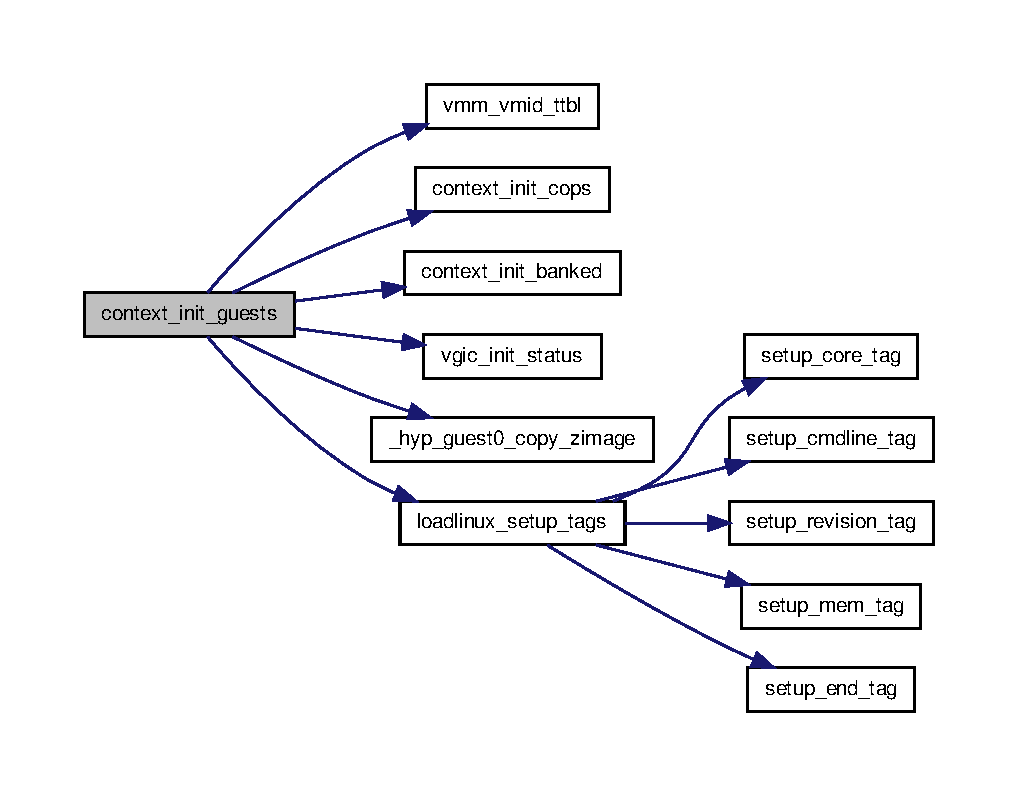
\includegraphics[width=350pt]{context_8h_a0abdd106a2b654464230b622b4c9877e_cgraph}
\end{center}
\end{figure}


\hypertarget{context_8h_ad48a9977fdb537cc020b451e08dfc590}{\index{context.\-h@{context.\-h}!context\-\_\-last\-\_\-vmid@{context\-\_\-last\-\_\-vmid}}
\index{context\-\_\-last\-\_\-vmid@{context\-\_\-last\-\_\-vmid}!context.h@{context.\-h}}
\subsubsection[{context\-\_\-last\-\_\-vmid}]{\setlength{\rightskip}{0pt plus 5cm}{\bf vmid\-\_\-t} {\bf context\-\_\-last\-\_\-vmid} (
\begin{DoxyParamCaption}
\item[{void}]{}
\end{DoxyParamCaption}
)}}\label{context_8h_ad48a9977fdb537cc020b451e08dfc590}


\-Definition at line 544 of file context.\-c.


\begin{DoxyCode}
{
    /* FIXME:Hardcoded for now */
    return 1;
}
\end{DoxyCode}
\hypertarget{context_8h_a5719d5d4a8d98b9784d0f24a2023f05f}{\index{context.\-h@{context.\-h}!context\-\_\-next\-\_\-vmid@{context\-\_\-next\-\_\-vmid}}
\index{context\-\_\-next\-\_\-vmid@{context\-\_\-next\-\_\-vmid}!context.h@{context.\-h}}
\subsubsection[{context\-\_\-next\-\_\-vmid}]{\setlength{\rightskip}{0pt plus 5cm}{\bf vmid\-\_\-t} {\bf context\-\_\-next\-\_\-vmid} (
\begin{DoxyParamCaption}
\item[{{\bf vmid\-\_\-t}}]{ofvmid}
\end{DoxyParamCaption}
)}}\label{context_8h_a5719d5d4a8d98b9784d0f24a2023f05f}


\-Definition at line 550 of file context.\-c.


\begin{DoxyCode}
{
    vmid_t next = VMID_INVALID;
    if ( ofvmid == VMID_INVALID ) {
        next = context_first_vmid();
    } else if ( ofvmid < context_last_vmid() ) {
        /* FIXME:Hardcoded */
        next = ofvmid + 1;
    }
    return next;
}
\end{DoxyCode}


\-Here is the call graph for this function\-:
\nopagebreak
\begin{figure}[H]
\begin{center}
\leavevmode
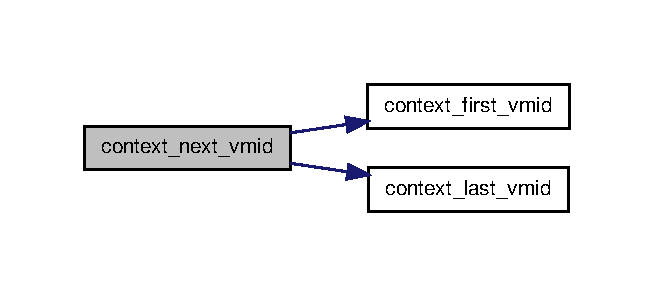
\includegraphics[width=314pt]{context_8h_a5719d5d4a8d98b9784d0f24a2023f05f_cgraph}
\end{center}
\end{figure}


\hypertarget{context_8h_a77fe269a194f9dcfcd0a599a9b6e3bfb}{\index{context.\-h@{context.\-h}!context\-\_\-perform\-\_\-switch@{context\-\_\-perform\-\_\-switch}}
\index{context\-\_\-perform\-\_\-switch@{context\-\_\-perform\-\_\-switch}!context.h@{context.\-h}}
\subsubsection[{context\-\_\-perform\-\_\-switch}]{\setlength{\rightskip}{0pt plus 5cm}{\bf hvmm\-\_\-status\-\_\-t} {\bf context\-\_\-perform\-\_\-switch} (
\begin{DoxyParamCaption}
\item[{void}]{}
\end{DoxyParamCaption}
)}}\label{context_8h_a77fe269a194f9dcfcd0a599a9b6e3bfb}


\-Definition at line 419 of file context.\-c.


\begin{DoxyCode}
{
    hvmm_status_t result = HVMM_STATUS_IGNORED;

    if ( _current_guest_vmid == VMID_INVALID ) {
        printh("context: launching the first guest\n");
        /* very first time, to the default first guest */
        result = context_perform_switch_to_guest_regs( 0, _next_guest_vmid );
        /* DOES NOT COME BACK HERE */
    } else if ( _next_guest_vmid != VMID_INVALID && _current_guest_vmid != 
      _next_guest_vmid ) {
        struct arch_regs *regs = trap_saved_regs();
        if ( (regs->cpsr & 0x1F) != 0x1A ) {
            printh("curr: %x\n", _current_guest_vmid);
            printh("next: %x\n", _next_guest_vmid);

            /* Only if not from Hyp */
            result = context_perform_switch_to_guest_regs( regs, 
      _next_guest_vmid );
            _next_guest_vmid = VMID_INVALID;
        }
    } else {
        /* Staying at the currently active guest. Flush out queued virqs since
       we didn't have a chance to switch the context, where virq flush takes place, 
       this time */
        vgic_flush_virqs(_current_guest_vmid);
    }

    _switch_locked = 0;
    return result;
}
\end{DoxyCode}


\-Here is the call graph for this function\-:
\nopagebreak
\begin{figure}[H]
\begin{center}
\leavevmode
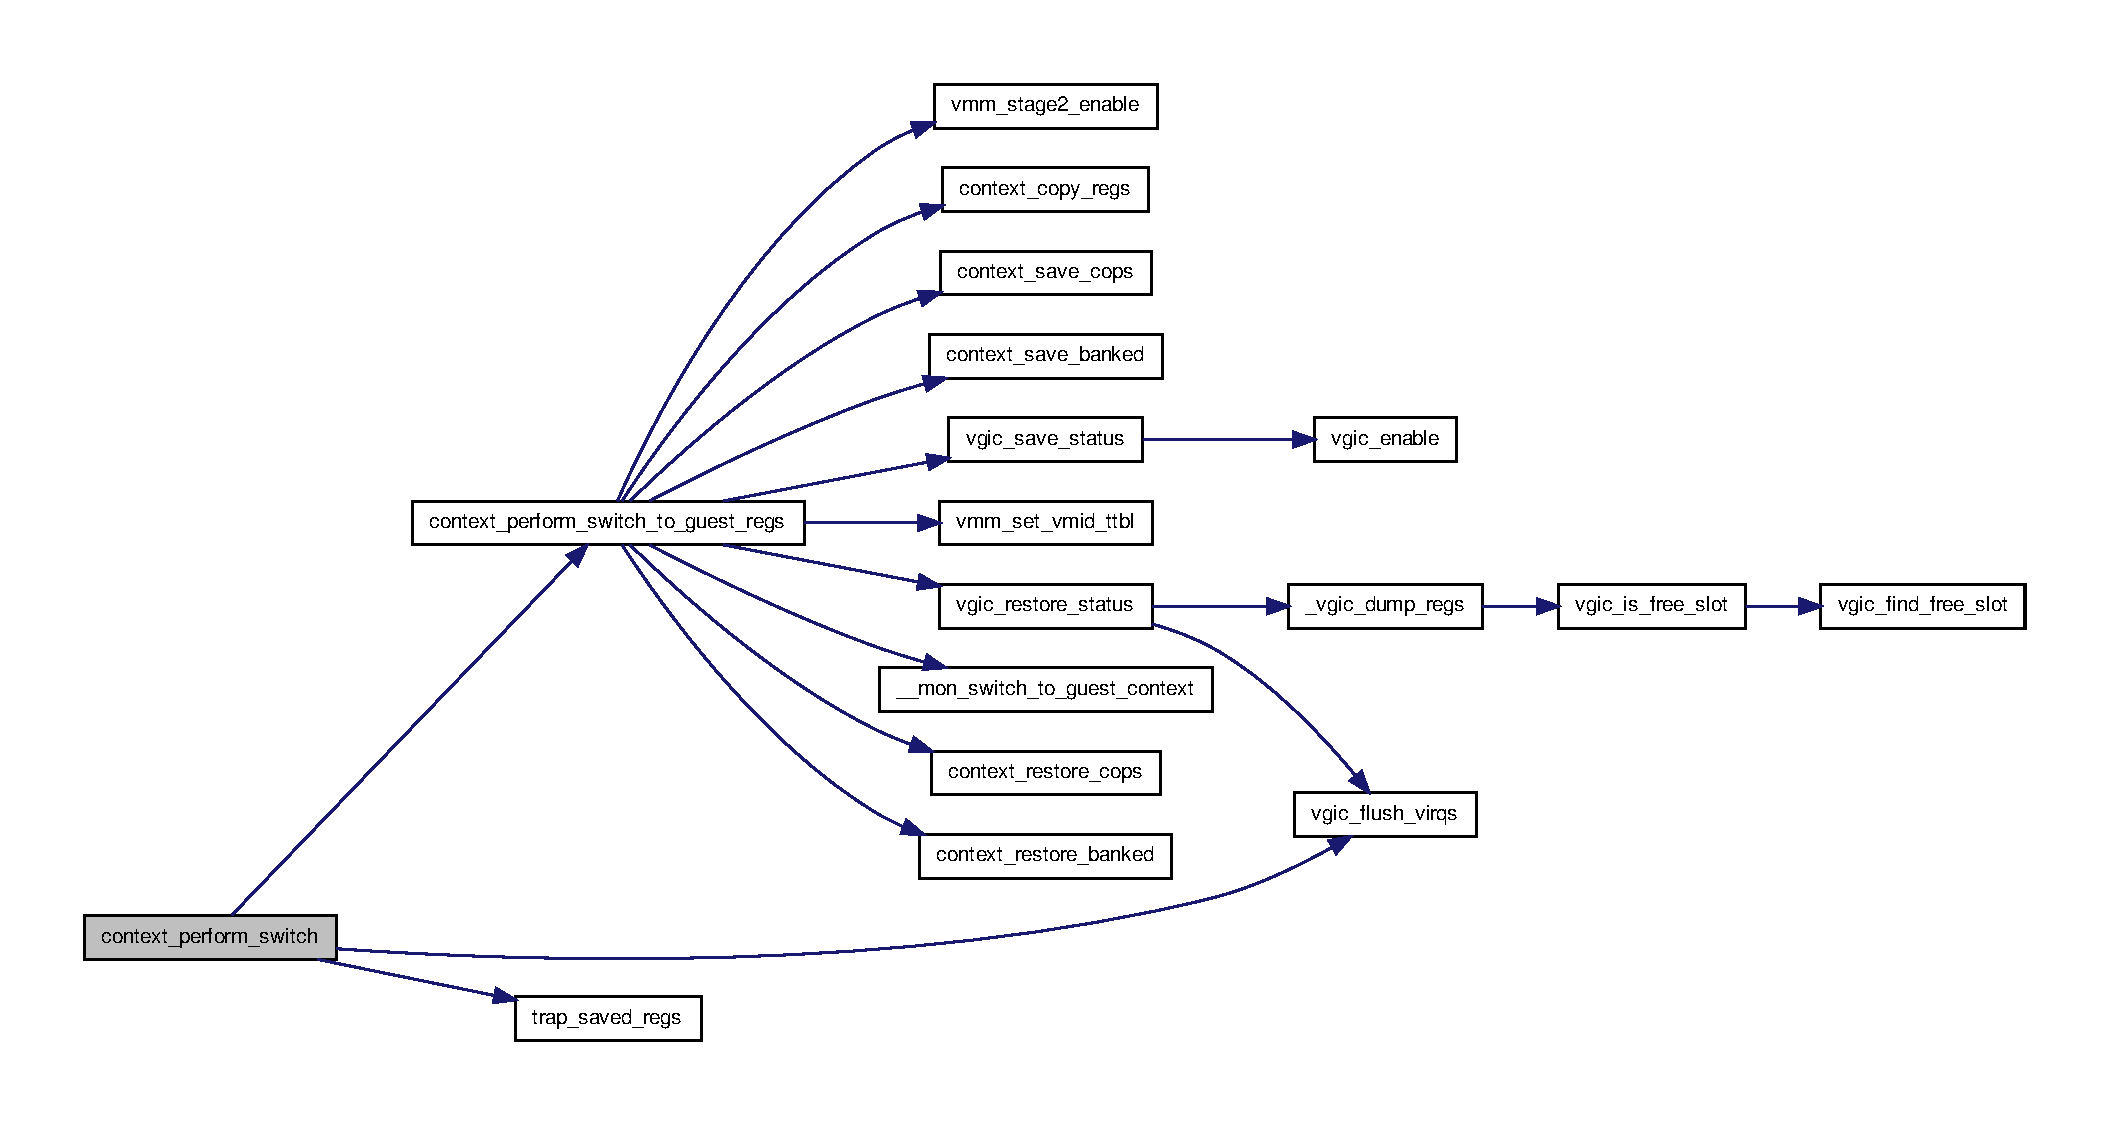
\includegraphics[width=350pt]{context_8h_a77fe269a194f9dcfcd0a599a9b6e3bfb_cgraph}
\end{center}
\end{figure}


\hypertarget{context_8h_a39db644c82cc9c99ef78feb58d57b58c}{\index{context.\-h@{context.\-h}!context\-\_\-switch\-\_\-to\-\_\-initial\-\_\-guest@{context\-\_\-switch\-\_\-to\-\_\-initial\-\_\-guest}}
\index{context\-\_\-switch\-\_\-to\-\_\-initial\-\_\-guest@{context\-\_\-switch\-\_\-to\-\_\-initial\-\_\-guest}!context.h@{context.\-h}}
\subsubsection[{context\-\_\-switch\-\_\-to\-\_\-initial\-\_\-guest}]{\setlength{\rightskip}{0pt plus 5cm}void {\bf context\-\_\-switch\-\_\-to\-\_\-initial\-\_\-guest} (
\begin{DoxyParamCaption}
\item[{void}]{}
\end{DoxyParamCaption}
)}}\label{context_8h_a39db644c82cc9c99ef78feb58d57b58c}


\-Definition at line 447 of file context.\-c.


\begin{DoxyCode}
{
    struct hyp_guest_context *context = 0;
    struct arch_regs *regs = 0;

    uart_print("[hyp] switch_to_initial_guest:\n\r");

    /* Select the first guest context to switch to. */
    _current_guest_vmid = VMID_INVALID;
    context = &guest_contexts[0];

    /* Dump the initial register values of the guest for debugging purpose */
    regs = &context->regs;
    context_dump_regs( regs );

    /* Context Switch with current context == none */
    context_switchto(0);
    context_perform_switch();
}
\end{DoxyCode}


\-Here is the call graph for this function\-:
\nopagebreak
\begin{figure}[H]
\begin{center}
\leavevmode
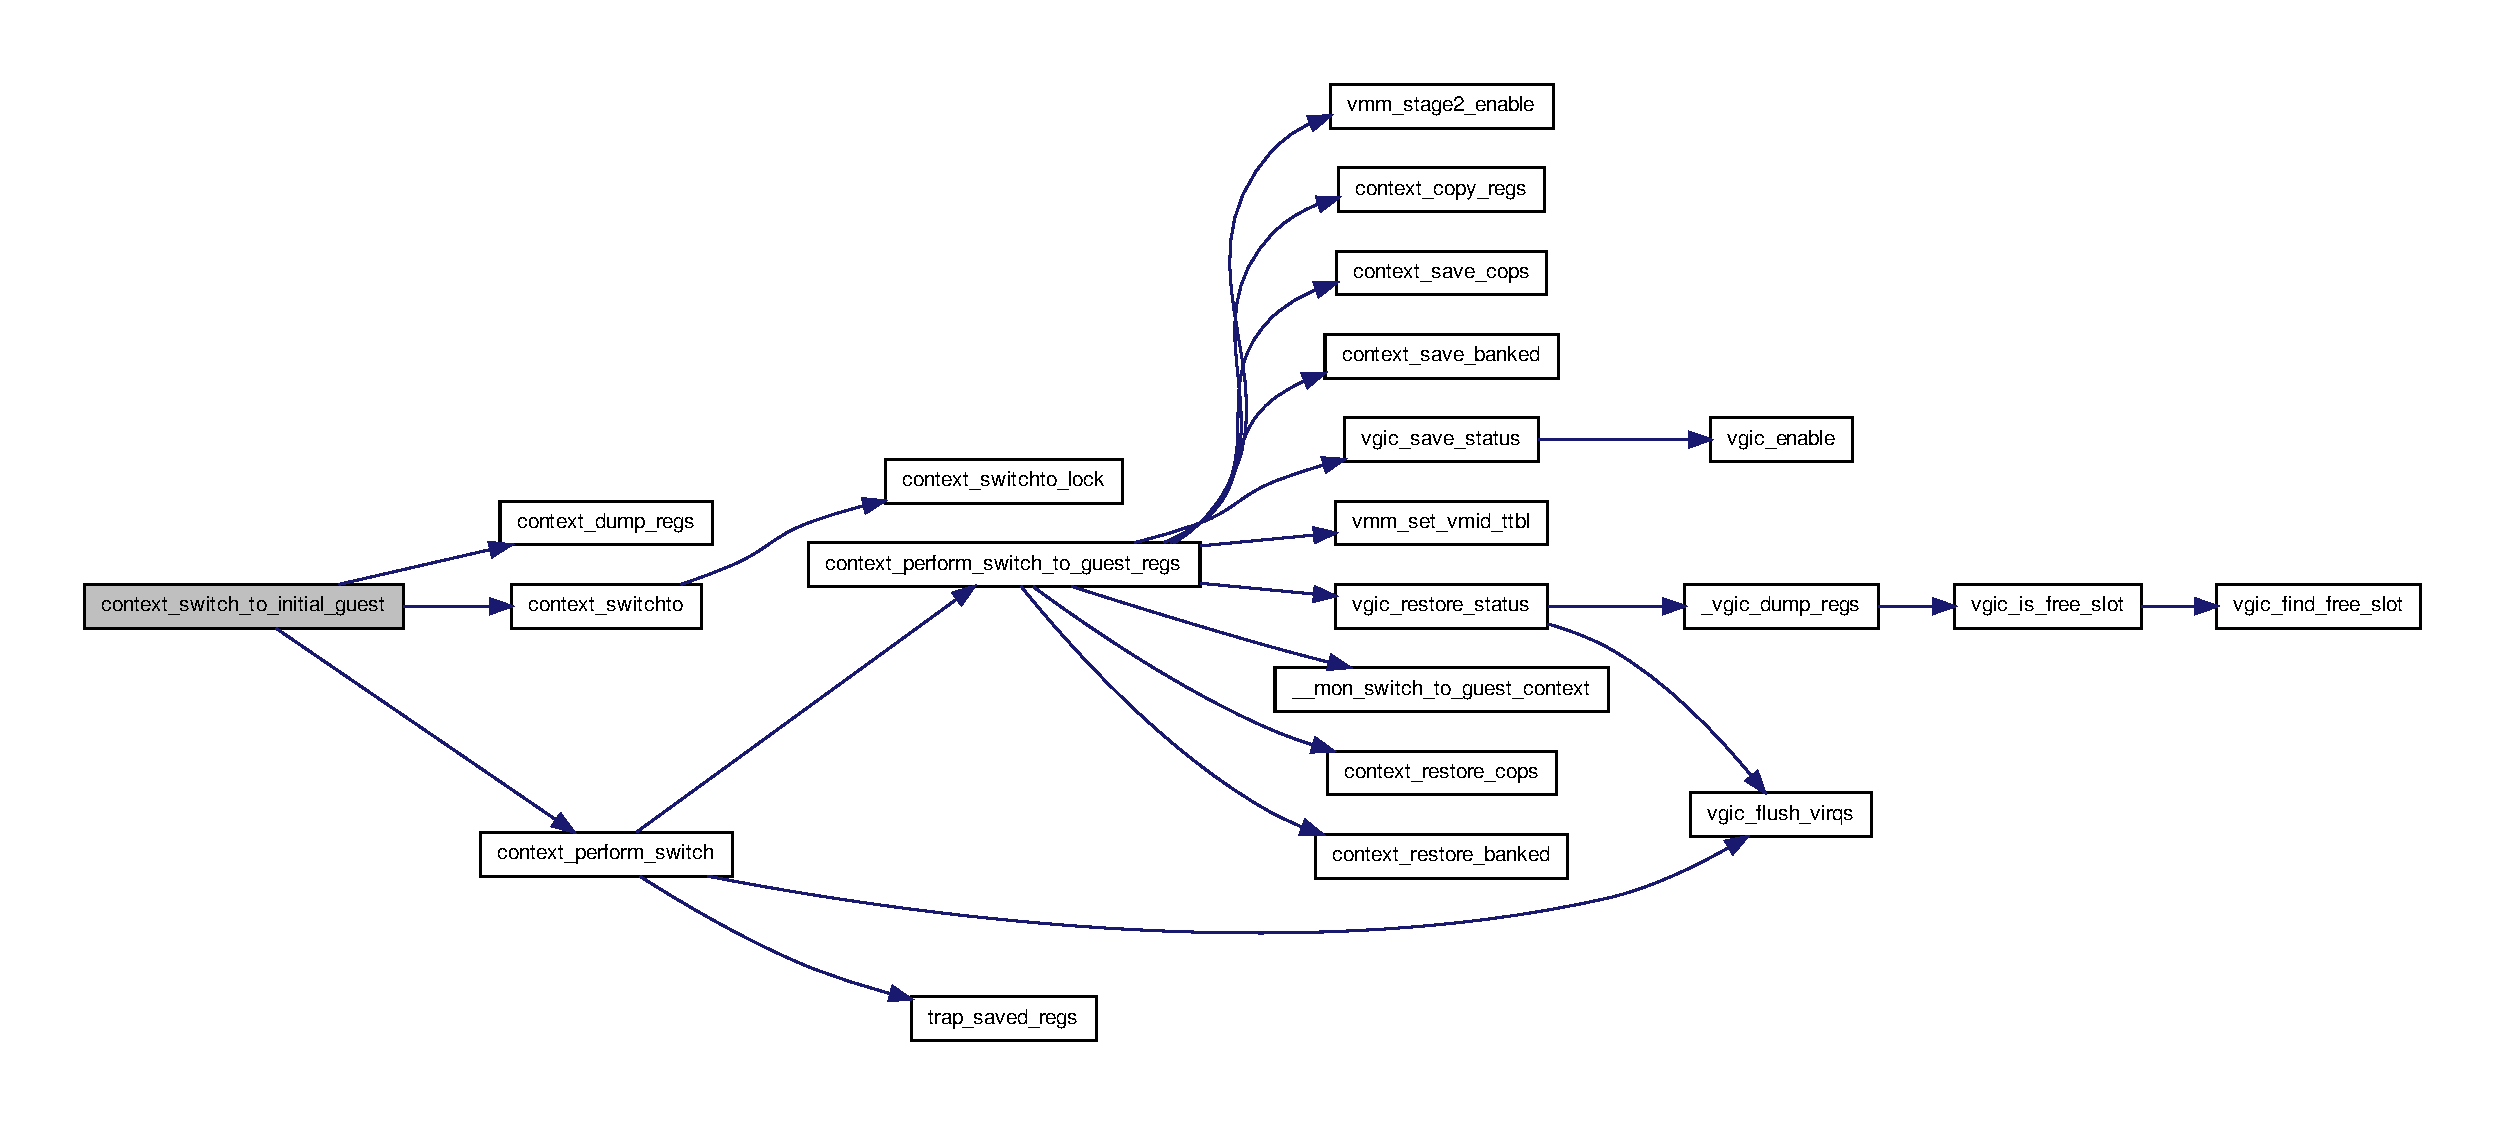
\includegraphics[width=350pt]{context_8h_a39db644c82cc9c99ef78feb58d57b58c_cgraph}
\end{center}
\end{figure}


\hypertarget{context_8h_aaa75f8a973764763b44ca823e02f4406}{\index{context.\-h@{context.\-h}!context\-\_\-switchto@{context\-\_\-switchto}}
\index{context\-\_\-switchto@{context\-\_\-switchto}!context.h@{context.\-h}}
\subsubsection[{context\-\_\-switchto}]{\setlength{\rightskip}{0pt plus 5cm}{\bf hvmm\-\_\-status\-\_\-t} {\bf context\-\_\-switchto} (
\begin{DoxyParamCaption}
\item[{{\bf vmid\-\_\-t}}]{vmid}
\end{DoxyParamCaption}
)}}\label{context_8h_aaa75f8a973764763b44ca823e02f4406}


\-Definition at line 572 of file context.\-c.


\begin{DoxyCode}
{
    return context_switchto_lock(vmid, 0);
}
\end{DoxyCode}


\-Here is the call graph for this function\-:
\nopagebreak
\begin{figure}[H]
\begin{center}
\leavevmode
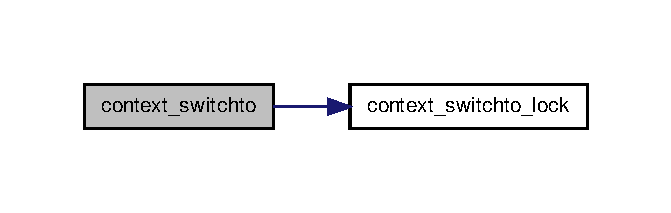
\includegraphics[width=322pt]{context_8h_aaa75f8a973764763b44ca823e02f4406_cgraph}
\end{center}
\end{figure}


\hypertarget{context_8h_a00b56df45d0ef16d93040b667bb025ef}{\index{context.\-h@{context.\-h}!context\-\_\-switchto\-\_\-lock@{context\-\_\-switchto\-\_\-lock}}
\index{context\-\_\-switchto\-\_\-lock@{context\-\_\-switchto\-\_\-lock}!context.h@{context.\-h}}
\subsubsection[{context\-\_\-switchto\-\_\-lock}]{\setlength{\rightskip}{0pt plus 5cm}{\bf hvmm\-\_\-status\-\_\-t} {\bf context\-\_\-switchto\-\_\-lock} (
\begin{DoxyParamCaption}
\item[{{\bf vmid\-\_\-t}}]{vmid, }
\item[{{\bf uint8\-\_\-t}}]{locked}
\end{DoxyParamCaption}
)}}\label{context_8h_a00b56df45d0ef16d93040b667bb025ef}


\-Definition at line 577 of file context.\-c.


\begin{DoxyCode}
{
    hvmm_status_t result = HVMM_STATUS_IGNORED;

    HVMM_TRACE_ENTER();

    /* valid and not current vmid, switch */
    if (_switch_locked == 0) {
        if ( !_valid_vmid(vmid) ) {
            result = HVMM_STATUS_BAD_ACCESS;
        } else {
            _next_guest_vmid = vmid;
            result = HVMM_STATUS_SUCCESS;

            printh("switching to vmid: %x\n", (uint32_t)vmid);
        }
    } else {
        printh("context: next vmid locked to %d\n", _next_guest_vmid );
    }

    if ( locked )
        _switch_locked = locked;

    HVMM_TRACE_EXIT();
    return result;
}
\end{DoxyCode}
\hypertarget{context_8h_a3fd5aa68bf14823442fcc5fda4cb6a51}{\index{context.\-h@{context.\-h}!context\-\_\-waiting\-\_\-vmid@{context\-\_\-waiting\-\_\-vmid}}
\index{context\-\_\-waiting\-\_\-vmid@{context\-\_\-waiting\-\_\-vmid}!context.h@{context.\-h}}
\subsubsection[{context\-\_\-waiting\-\_\-vmid}]{\setlength{\rightskip}{0pt plus 5cm}{\bf vmid\-\_\-t} {\bf context\-\_\-waiting\-\_\-vmid} (
\begin{DoxyParamCaption}
\item[{void}]{}
\end{DoxyParamCaption}
)}}\label{context_8h_a3fd5aa68bf14823442fcc5fda4cb6a51}


\-Definition at line 567 of file context.\-c.


\begin{DoxyCode}
{
    return _next_guest_vmid;
}
\end{DoxyCode}
\hypertarget{context_8h_a83895de158b7efc9456e7475528e42d4}{\index{context.\-h@{context.\-h}!start\-\_\-guest\-\_\-os@{start\-\_\-guest\-\_\-os}}
\index{start\-\_\-guest\-\_\-os@{start\-\_\-guest\-\_\-os}!context.h@{context.\-h}}
\subsubsection[{start\-\_\-guest\-\_\-os}]{\setlength{\rightskip}{0pt plus 5cm}void {\bf start\-\_\-guest\-\_\-os} (
\begin{DoxyParamCaption}
\item[{void}]{}
\end{DoxyParamCaption}
)}}\label{context_8h_a83895de158b7efc9456e7475528e42d4}


\-Definition at line 604 of file context.\-c.


\begin{DoxyCode}
{
    init_print();

    hvmm_status_t ret = HVMM_STATUS_UNKNOWN_ERROR;
    printh("[%s : %d] Starting...\n", __FUNCTION__, __LINE__);

    /* Initialize Memory Management */
    ret = hvmm_mm_init();

    /* Initialize Interrupt Management */
    ret = hvmm_interrupt_init();
    if ( ret != HVMM_STATUS_SUCCESS ) {
        uart_print("[hyp_main] interrupt initialization failed...\n\r");
    }

    /* Initialize Guests */
    context_init_guests();

    /* Initialize Virtual Devices */
    vdev_init();

    /* Virtual GIC Distributor */
    printh( "tests: Registering sample vdev:'vgicd' at %x\n", CFG_GIC_BASE_PA |
       GIC_OFFSET_GICD);
    vdev_gicd_init(CFG_GIC_BASE_PA | GIC_OFFSET_GICD);

    /* Initialize PIRQ to VIRQ mapping */
    virqmap_init();

    /* Start Scheduling */
    scheduler_test_scheduling();

    /* Begin running test code for newly implemented features */
    hvmm_tests_main();

    /* Print Banner */
    printH("%s", BANNER_STRING);

    /* Switch to the first guest */
    context_switch_to_initial_guest();

    /* The code flow must not reach here */
    uart_print("[hyp_main] ERROR: CODE MUST NOT REACH HERE\n\r");
    hyp_abort_infinite();
}
\end{DoxyCode}


\-Here is the call graph for this function\-:
\nopagebreak
\begin{figure}[H]
\begin{center}
\leavevmode
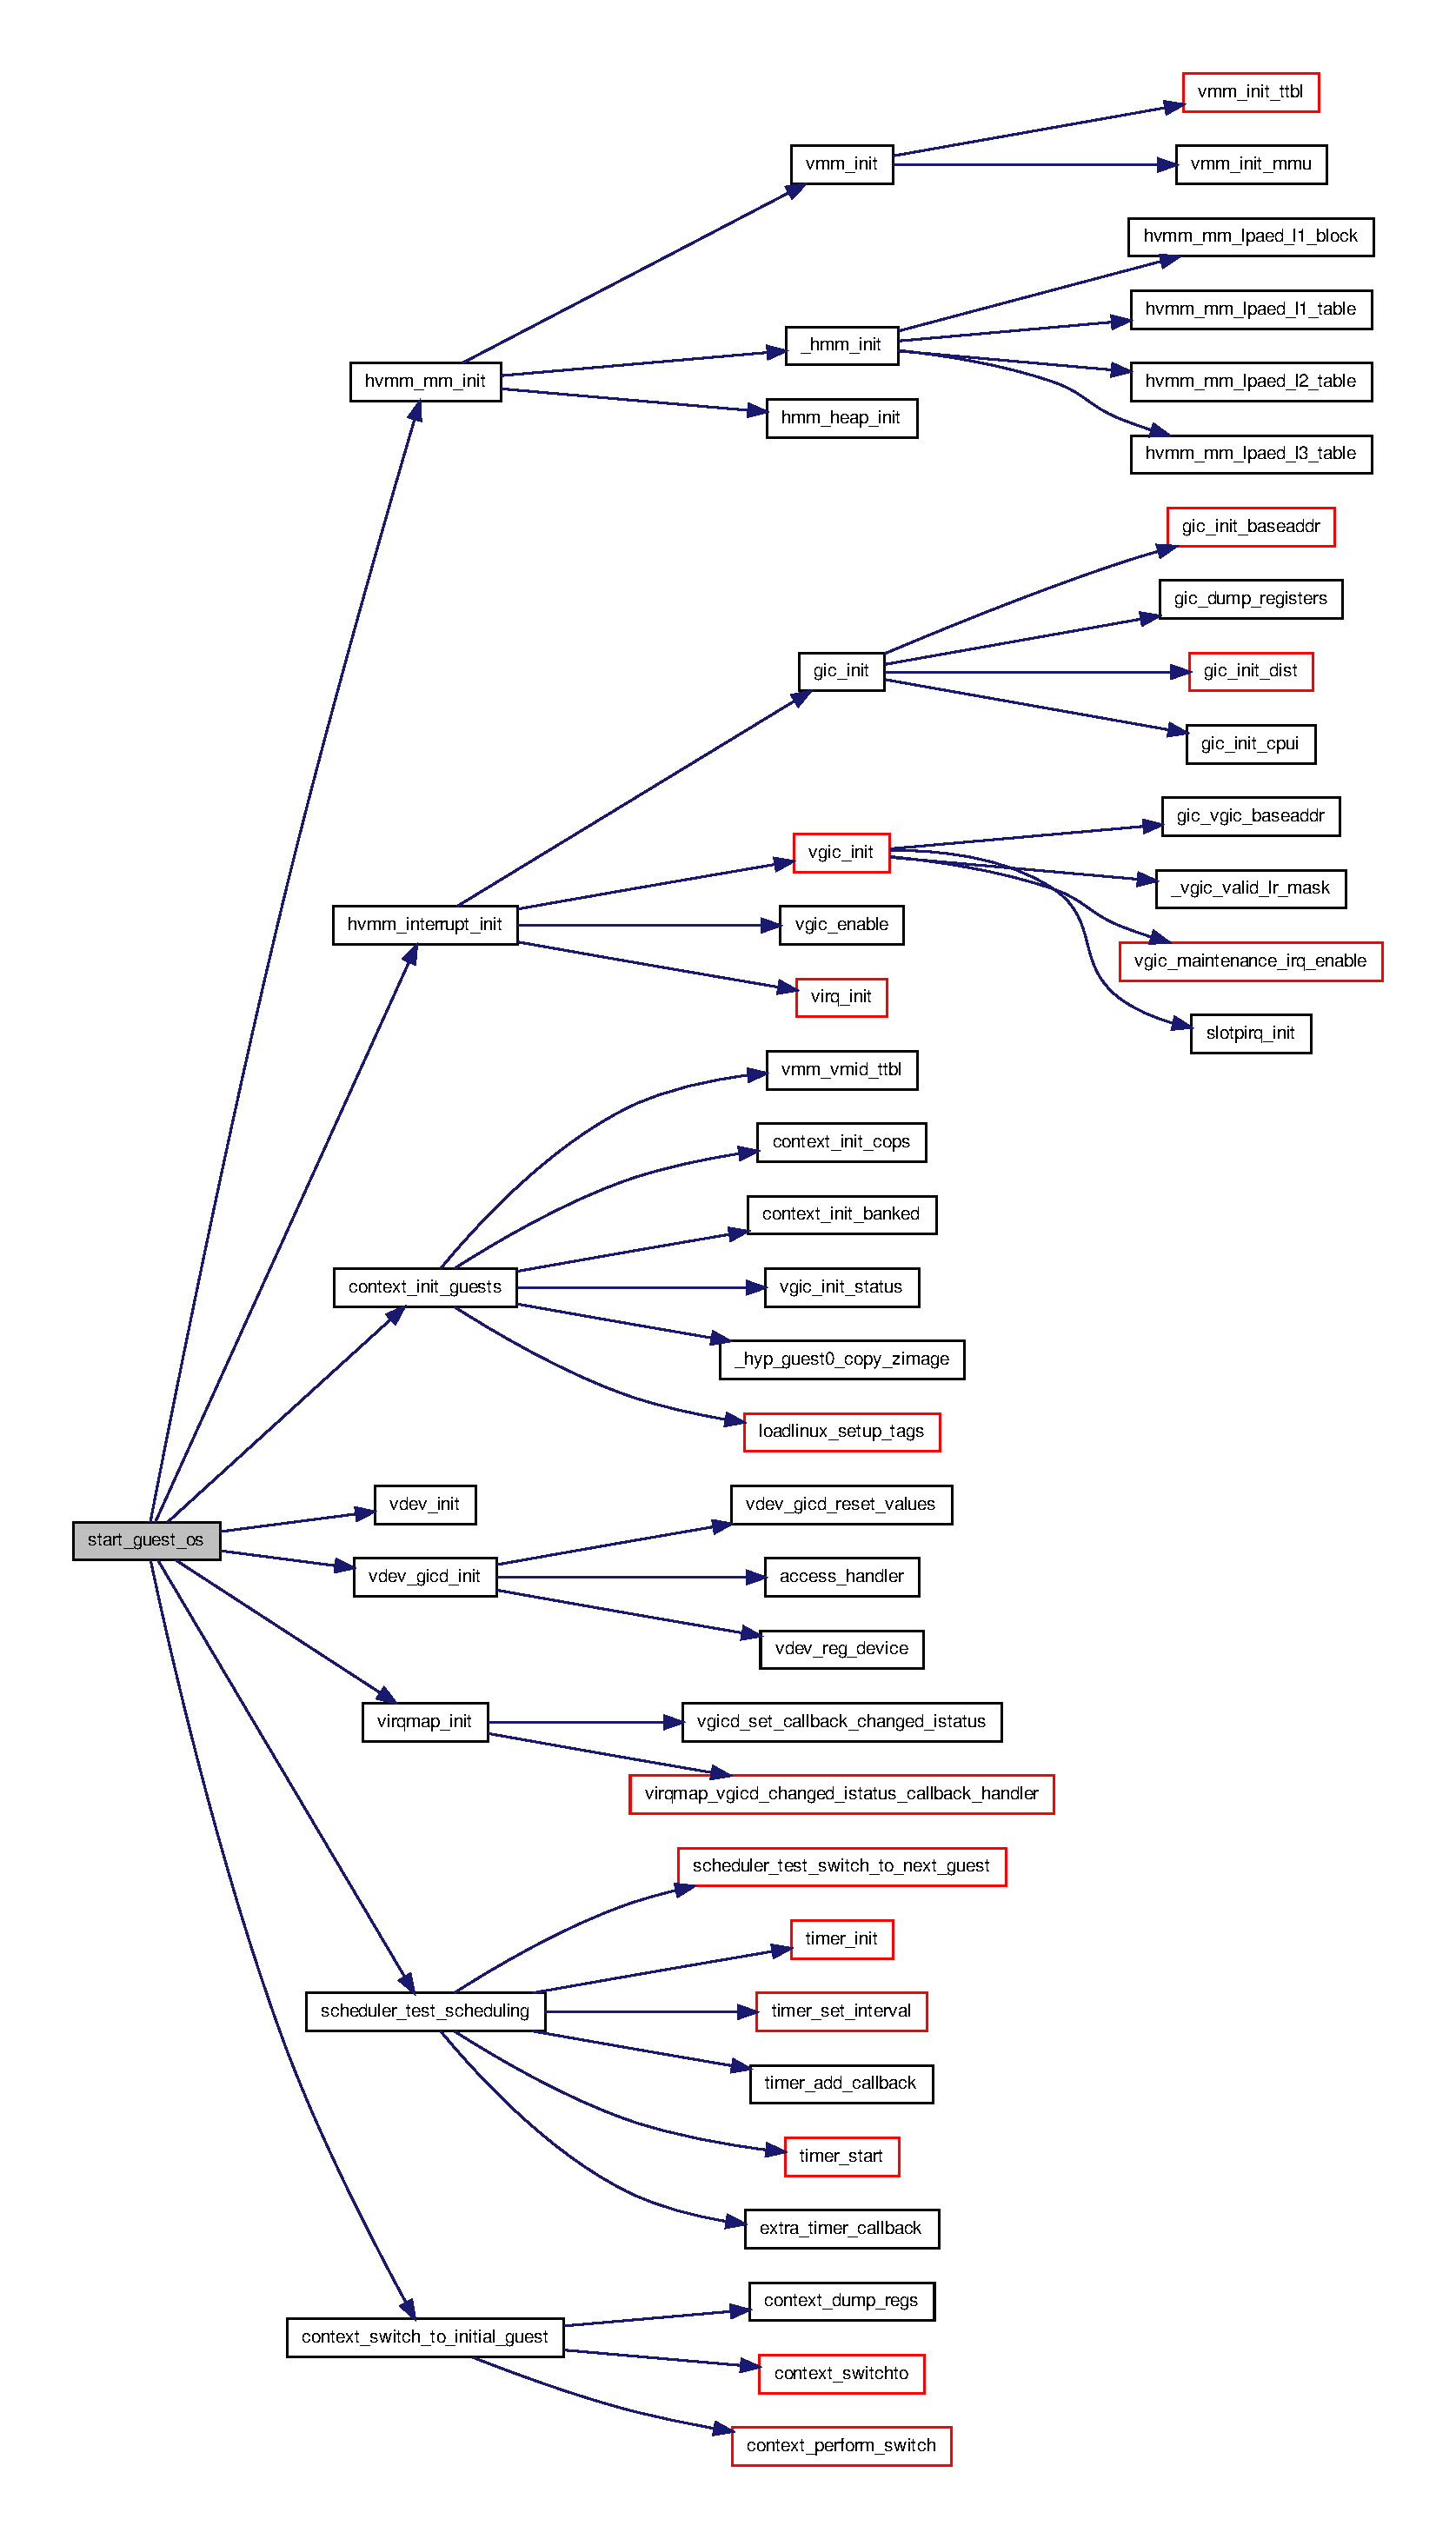
\includegraphics[height=550pt]{context_8h_a83895de158b7efc9456e7475528e42d4_cgraph}
\end{center}
\end{figure}




\subsection{\-Variable \-Documentation}
\hypertarget{context_8h_a06b520051af1c5c2e4d477566b23baa7}{\index{context.\-h@{context.\-h}!\-\_\-\-\_\-attribute@{\-\_\-\-\_\-attribute}}
\index{\-\_\-\-\_\-attribute@{\-\_\-\-\_\-attribute}!context.h@{context.\-h}}
\subsubsection[{\-\_\-\-\_\-attribute}]{\setlength{\rightskip}{0pt plus 5cm}struct {\bf arch\-\_\-regs\-\_\-cop}  {\bf \-\_\-\-\_\-attribute}}}\label{context_8h_a06b520051af1c5c2e4d477566b23baa7}
\hypertarget{context_8h_a0d1814f5edf1360a76b54ac386be5e85}{\index{context.\-h@{context.\-h}!cpsr@{cpsr}}
\index{cpsr@{cpsr}!context.h@{context.\-h}}
\subsubsection[{cpsr}]{\setlength{\rightskip}{0pt plus 5cm}{\bf uint32\-\_\-t} {\bf cpsr}}}\label{context_8h_a0d1814f5edf1360a76b54ac386be5e85}


\-Definition at line 22 of file context.\-h.

\hypertarget{context_8h_a3397c2bbf4a3049cf5bca2831ada10b8}{\index{context.\-h@{context.\-h}!gpr@{gpr}}
\index{gpr@{gpr}!context.h@{context.\-h}}
\subsubsection[{gpr}]{\setlength{\rightskip}{0pt plus 5cm}{\bf uint32\-\_\-t} {\bf gpr}\mbox{[}{\bf \-A\-R\-C\-H\-\_\-\-R\-E\-G\-S\-\_\-\-N\-U\-M\-\_\-\-G\-P\-R}\mbox{]}}}\label{context_8h_a3397c2bbf4a3049cf5bca2831ada10b8}


\-Definition at line 25 of file context.\-h.

\hypertarget{context_8h_a6ced3f4007bb60daf12191c058e55b8c}{\index{context.\-h@{context.\-h}!lr@{lr}}
\index{lr@{lr}!context.h@{context.\-h}}
\subsubsection[{lr}]{\setlength{\rightskip}{0pt plus 5cm}{\bf uint32\-\_\-t} {\bf lr}}}\label{context_8h_a6ced3f4007bb60daf12191c058e55b8c}


\-Definition at line 24 of file context.\-h.

\hypertarget{context_8h_a27468faba76ab3fb5458fb06c0f2af8a}{\index{context.\-h@{context.\-h}!pc@{pc}}
\index{pc@{pc}!context.h@{context.\-h}}
\subsubsection[{pc}]{\setlength{\rightskip}{0pt plus 5cm}syntax unified arch\-\_\-extension sec arch\-\_\-extension virt text align \-S\-C\-R {\bf r10} bic ldr {\bf r11} mcr {\bf isb} \-Use {\bf monitor\-\_\-secure\-\_\-vectors} as temporary \-Hyp exception vector for \-Hyp mode entrance ldr {\bf return} in \-N\-S state movs {\bf lr} {\bf elr\-\_\-hyp} mov {\bf pc}}}\label{context_8h_a27468faba76ab3fb5458fb06c0f2af8a}


\-Definition at line 23 of file context.\-h.


\hypertarget{generic__timer_8c}{\section{generic\-\_\-timer/generic\-\_\-timer.c \-File \-Reference}
\label{generic__timer_8c}\index{generic\-\_\-timer/generic\-\_\-timer.\-c@{generic\-\_\-timer/generic\-\_\-timer.\-c}}
}
{\ttfamily \#include $<$generic\-\_\-timer.\-h$>$}\*
{\ttfamily \#include $<$hvmm\-\_\-trace.\-h$>$}\*
{\ttfamily \#include \char`\"{}generic\-\_\-timer\-\_\-regs.\-h\char`\"{}}\*
{\ttfamily \#include $<$config/cfg\-\_\-platform.\-h$>$}\*
\-Include dependency graph for generic\-\_\-timer.\-c\-:
\nopagebreak
\begin{figure}[H]
\begin{center}
\leavevmode
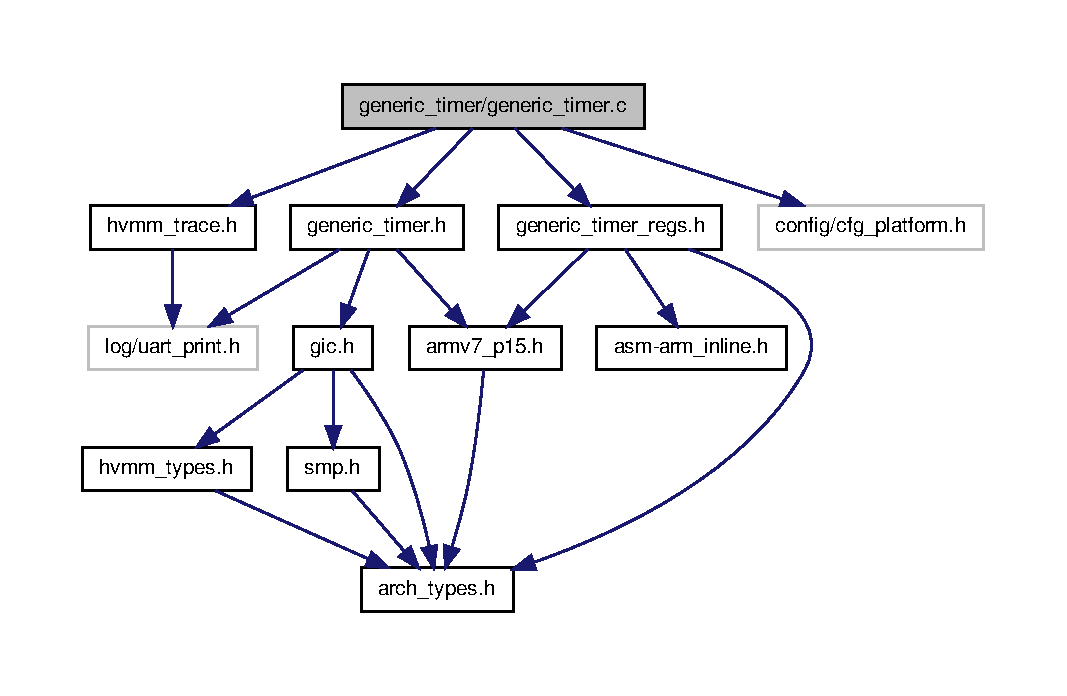
\includegraphics[width=350pt]{generic__timer_8c__incl}
\end{center}
\end{figure}
\subsection*{\-Functions}
\begin{DoxyCompactItemize}
\item 
static void \hyperlink{generic__timer_8c_a1ec3de997b7552597b2ba32e6068e069}{\-\_\-generic\-\_\-timer\-\_\-hyp\-\_\-irq\-\_\-handler} (int irq, void $\ast$\hyperlink{vdev__timer_8c_a514d7f36beee4b3e39da305e12d39d0a}{regs}, void $\ast$pdata)
\item 
\hyperlink{hvmm__types_8h_a39d593b2c97852f566d7472b76ab7ba2}{hvmm\-\_\-status\-\_\-t} \hyperlink{generic__timer_8c_abc62af83e49119c8a1e22606340fcc31}{generic\-\_\-timer\-\_\-init} ()
\item 
\hyperlink{hvmm__types_8h_a39d593b2c97852f566d7472b76ab7ba2}{hvmm\-\_\-status\-\_\-t} \hyperlink{generic__timer_8c_a9c827fc2504de623842afa015a0791e2}{generic\-\_\-timer\-\_\-set\-\_\-tval} (\hyperlink{generic__timer_8h_a1070f2e7b73c8b78be519eb9dc26e5bc}{generic\-\_\-timer\-\_\-type\-\_\-t} type, \hyperlink{arch__types_8h_a435d1572bf3f880d55459d9805097f62}{uint32\-\_\-t} tval)
\item 
\hyperlink{hvmm__types_8h_a39d593b2c97852f566d7472b76ab7ba2}{hvmm\-\_\-status\-\_\-t} \hyperlink{generic__timer_8c_ac31d0e77e798fb55de96b4ff320c1a17}{generic\-\_\-timer\-\_\-enable\-\_\-int} (\hyperlink{generic__timer_8h_a1070f2e7b73c8b78be519eb9dc26e5bc}{generic\-\_\-timer\-\_\-type\-\_\-t} type)
\item 
\hyperlink{hvmm__types_8h_a39d593b2c97852f566d7472b76ab7ba2}{hvmm\-\_\-status\-\_\-t} \hyperlink{generic__timer_8c_ae4cbbf157ccf4126af25918bfc239918}{generic\-\_\-timer\-\_\-disable\-\_\-int} (\hyperlink{generic__timer_8h_a1070f2e7b73c8b78be519eb9dc26e5bc}{generic\-\_\-timer\-\_\-type\-\_\-t} type)
\item 
\hyperlink{hvmm__types_8h_a39d593b2c97852f566d7472b76ab7ba2}{hvmm\-\_\-status\-\_\-t} \hyperlink{generic__timer_8c_a7adf47a410958220c1df75a9edbc253c}{generic\-\_\-timer\-\_\-enable\-\_\-irq} (\hyperlink{generic__timer_8h_a1070f2e7b73c8b78be519eb9dc26e5bc}{generic\-\_\-timer\-\_\-type\-\_\-t} type)
\item 
\hyperlink{hvmm__types_8h_a39d593b2c97852f566d7472b76ab7ba2}{hvmm\-\_\-status\-\_\-t} \hyperlink{generic__timer_8c_a26fcbba99e1dbf1ac9e06b91e3bc3ab6}{generic\-\_\-timer\-\_\-set\-\_\-callback} (\hyperlink{generic__timer_8h_a1070f2e7b73c8b78be519eb9dc26e5bc}{generic\-\_\-timer\-\_\-type\-\_\-t} type, \hyperlink{generic__timer_8h_abc1b1dc35e32f7380f3f22624cb3b6e0}{generic\-\_\-timer\-\_\-callback\-\_\-t} callback)
\end{DoxyCompactItemize}
\subsection*{\-Variables}
\begin{DoxyCompactItemize}
\item 
static \hyperlink{arch__types_8h_a435d1572bf3f880d55459d9805097f62}{uint32\-\_\-t} \hyperlink{generic__timer_8c_a5b94dd32413eab57ab72bb4b759fc703}{\-\_\-timer\-\_\-irqs} \mbox{[}\hyperlink{generic__timer_8h_a1070f2e7b73c8b78be519eb9dc26e5bca2a64bfa046f4766b301a15628ab6e764}{\-G\-E\-N\-E\-R\-I\-C\-\_\-\-T\-I\-M\-E\-R\-\_\-\-N\-U\-M\-\_\-\-T\-Y\-P\-E\-S}\mbox{]}
\item 
static \hyperlink{arch__types_8h_a435d1572bf3f880d55459d9805097f62}{uint32\-\_\-t} \hyperlink{generic__timer_8c_a05bc27c00841323051dcd14eaf0d95c4}{\-\_\-tvals} \mbox{[}\hyperlink{generic__timer_8h_a1070f2e7b73c8b78be519eb9dc26e5bca2a64bfa046f4766b301a15628ab6e764}{\-G\-E\-N\-E\-R\-I\-C\-\_\-\-T\-I\-M\-E\-R\-\_\-\-N\-U\-M\-\_\-\-T\-Y\-P\-E\-S}\mbox{]}
\item 
static \hyperlink{generic__timer_8h_abc1b1dc35e32f7380f3f22624cb3b6e0}{generic\-\_\-timer\-\_\-callback\-\_\-t} \hyperlink{generic__timer_8c_a793f595a9f49f888bb9f6a50fc960e93}{\-\_\-callback} \mbox{[}\hyperlink{generic__timer_8h_a1070f2e7b73c8b78be519eb9dc26e5bca2a64bfa046f4766b301a15628ab6e764}{\-G\-E\-N\-E\-R\-I\-C\-\_\-\-T\-I\-M\-E\-R\-\_\-\-N\-U\-M\-\_\-\-T\-Y\-P\-E\-S}\mbox{]}
\end{DoxyCompactItemize}


\subsection{\-Function \-Documentation}
\hypertarget{generic__timer_8c_a1ec3de997b7552597b2ba32e6068e069}{\index{generic\-\_\-timer.\-c@{generic\-\_\-timer.\-c}!\-\_\-generic\-\_\-timer\-\_\-hyp\-\_\-irq\-\_\-handler@{\-\_\-generic\-\_\-timer\-\_\-hyp\-\_\-irq\-\_\-handler}}
\index{\-\_\-generic\-\_\-timer\-\_\-hyp\-\_\-irq\-\_\-handler@{\-\_\-generic\-\_\-timer\-\_\-hyp\-\_\-irq\-\_\-handler}!generic_timer.c@{generic\-\_\-timer.\-c}}
\subsubsection[{\-\_\-generic\-\_\-timer\-\_\-hyp\-\_\-irq\-\_\-handler}]{\setlength{\rightskip}{0pt plus 5cm}static void {\bf \-\_\-generic\-\_\-timer\-\_\-hyp\-\_\-irq\-\_\-handler} (
\begin{DoxyParamCaption}
\item[{int}]{irq, }
\item[{void $\ast$}]{regs, }
\item[{void $\ast$}]{pdata}
\end{DoxyParamCaption}
)\hspace{0.3cm}{\ttfamily  \mbox{[}static\mbox{]}}}}\label{generic__timer_8c_a1ec3de997b7552597b2ba32e6068e069}


\-Definition at line 71 of file generic\-\_\-timer.\-c.


\begin{DoxyCode}
{
    _callback[GENERIC_TIMER_HYP](regs);
}
\end{DoxyCode}
\hypertarget{generic__timer_8c_ae4cbbf157ccf4126af25918bfc239918}{\index{generic\-\_\-timer.\-c@{generic\-\_\-timer.\-c}!generic\-\_\-timer\-\_\-disable\-\_\-int@{generic\-\_\-timer\-\_\-disable\-\_\-int}}
\index{generic\-\_\-timer\-\_\-disable\-\_\-int@{generic\-\_\-timer\-\_\-disable\-\_\-int}!generic_timer.c@{generic\-\_\-timer.\-c}}
\subsubsection[{generic\-\_\-timer\-\_\-disable\-\_\-int}]{\setlength{\rightskip}{0pt plus 5cm}{\bf hvmm\-\_\-status\-\_\-t} {\bf generic\-\_\-timer\-\_\-disable\-\_\-int} (
\begin{DoxyParamCaption}
\item[{{\bf generic\-\_\-timer\-\_\-type\-\_\-t}}]{type}
\end{DoxyParamCaption}
)}}\label{generic__timer_8c_ae4cbbf157ccf4126af25918bfc239918}


\-Definition at line 54 of file generic\-\_\-timer.\-c.


\begin{DoxyCode}
{
    uint32_t ctrl;
    hvmm_status_t result = HVMM_STATUS_UNSUPPORTED_FEATURE;

    if ( type == GENERIC_TIMER_HYP ) {
        ctrl = generic_timer_reg_read(GENERIC_TIMER_REG_HYP_CTRL);
        ctrl &= ~GENERIC_TIMER_CTRL_ENABLE;
        ctrl |= GENERIC_TIMER_CTRL_IMASK;

        generic_timer_reg_write(GENERIC_TIMER_REG_HYP_CTRL, ctrl);
        result = HVMM_STATUS_SUCCESS;
    }

    return result;
}
\end{DoxyCode}


\-Here is the call graph for this function\-:
\nopagebreak
\begin{figure}[H]
\begin{center}
\leavevmode
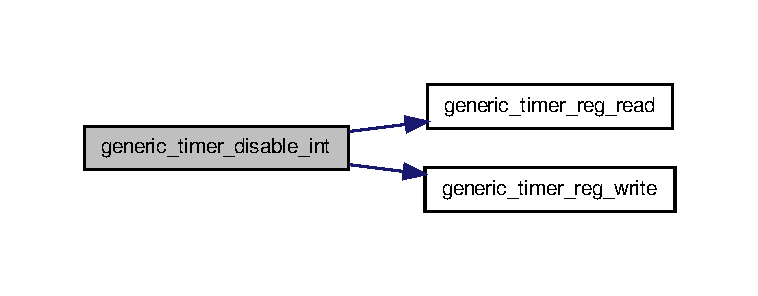
\includegraphics[width=350pt]{generic__timer_8c_ae4cbbf157ccf4126af25918bfc239918_cgraph}
\end{center}
\end{figure}


\hypertarget{generic__timer_8c_ac31d0e77e798fb55de96b4ff320c1a17}{\index{generic\-\_\-timer.\-c@{generic\-\_\-timer.\-c}!generic\-\_\-timer\-\_\-enable\-\_\-int@{generic\-\_\-timer\-\_\-enable\-\_\-int}}
\index{generic\-\_\-timer\-\_\-enable\-\_\-int@{generic\-\_\-timer\-\_\-enable\-\_\-int}!generic_timer.c@{generic\-\_\-timer.\-c}}
\subsubsection[{generic\-\_\-timer\-\_\-enable\-\_\-int}]{\setlength{\rightskip}{0pt plus 5cm}{\bf hvmm\-\_\-status\-\_\-t} {\bf generic\-\_\-timer\-\_\-enable\-\_\-int} (
\begin{DoxyParamCaption}
\item[{{\bf generic\-\_\-timer\-\_\-type\-\_\-t}}]{type}
\end{DoxyParamCaption}
)}}\label{generic__timer_8c_ac31d0e77e798fb55de96b4ff320c1a17}


\-Definition at line 37 of file generic\-\_\-timer.\-c.


\begin{DoxyCode}
{
    uint32_t ctrl;
    hvmm_status_t result = HVMM_STATUS_UNSUPPORTED_FEATURE;

    if ( type == GENERIC_TIMER_HYP ) {
        ctrl = generic_timer_reg_read(GENERIC_TIMER_REG_HYP_CTRL);
        ctrl |= GENERIC_TIMER_CTRL_ENABLE;      
        ctrl &= ~GENERIC_TIMER_CTRL_IMASK;
    
        generic_timer_reg_write(GENERIC_TIMER_REG_HYP_CTRL, ctrl);
        result = HVMM_STATUS_SUCCESS;
    }

    return result;
}
\end{DoxyCode}


\-Here is the call graph for this function\-:
\nopagebreak
\begin{figure}[H]
\begin{center}
\leavevmode
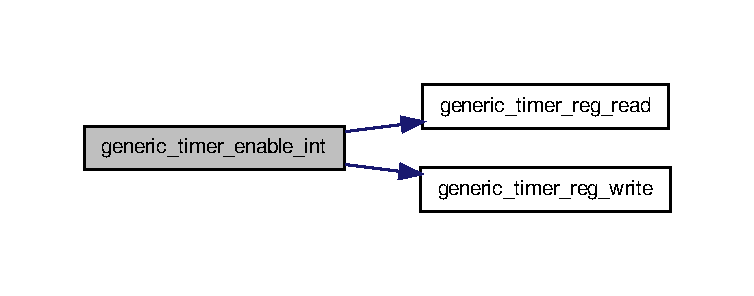
\includegraphics[width=350pt]{generic__timer_8c_ac31d0e77e798fb55de96b4ff320c1a17_cgraph}
\end{center}
\end{figure}


\hypertarget{generic__timer_8c_a7adf47a410958220c1df75a9edbc253c}{\index{generic\-\_\-timer.\-c@{generic\-\_\-timer.\-c}!generic\-\_\-timer\-\_\-enable\-\_\-irq@{generic\-\_\-timer\-\_\-enable\-\_\-irq}}
\index{generic\-\_\-timer\-\_\-enable\-\_\-irq@{generic\-\_\-timer\-\_\-enable\-\_\-irq}!generic_timer.c@{generic\-\_\-timer.\-c}}
\subsubsection[{generic\-\_\-timer\-\_\-enable\-\_\-irq}]{\setlength{\rightskip}{0pt plus 5cm}{\bf hvmm\-\_\-status\-\_\-t} {\bf generic\-\_\-timer\-\_\-enable\-\_\-irq} (
\begin{DoxyParamCaption}
\item[{{\bf generic\-\_\-timer\-\_\-type\-\_\-t}}]{type}
\end{DoxyParamCaption}
)}}\label{generic__timer_8c_a7adf47a410958220c1df75a9edbc253c}


\-Definition at line 76 of file generic\-\_\-timer.\-c.


\begin{DoxyCode}
{
    hvmm_status_t result = HVMM_STATUS_UNSUPPORTED_FEATURE;

    if ( type == GENERIC_TIMER_HYP ) {
        uint32_t irq = _timer_irqs[type];

        gic_test_set_irq_handler(irq, &_generic_timer_hyp_irq_handler, 0);

        gic_test_configure_irq(irq,
            GIC_INT_POLARITY_LEVEL, 
            gic_cpumask_current(),
            GIC_INT_PRIORITY_DEFAULT );

        result = HVMM_STATUS_SUCCESS;
    }
    return result;
}
\end{DoxyCode}


\-Here is the call graph for this function\-:
\nopagebreak
\begin{figure}[H]
\begin{center}
\leavevmode
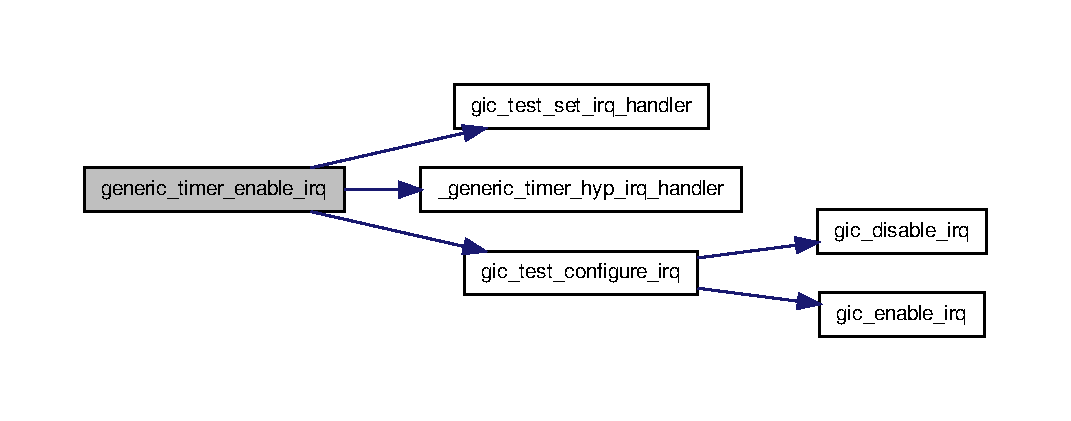
\includegraphics[width=350pt]{generic__timer_8c_a7adf47a410958220c1df75a9edbc253c_cgraph}
\end{center}
\end{figure}


\hypertarget{generic__timer_8c_abc62af83e49119c8a1e22606340fcc31}{\index{generic\-\_\-timer.\-c@{generic\-\_\-timer.\-c}!generic\-\_\-timer\-\_\-init@{generic\-\_\-timer\-\_\-init}}
\index{generic\-\_\-timer\-\_\-init@{generic\-\_\-timer\-\_\-init}!generic_timer.c@{generic\-\_\-timer.\-c}}
\subsubsection[{generic\-\_\-timer\-\_\-init}]{\setlength{\rightskip}{0pt plus 5cm}{\bf hvmm\-\_\-status\-\_\-t} {\bf generic\-\_\-timer\-\_\-init} (
\begin{DoxyParamCaption}
{}
\end{DoxyParamCaption}
)}}\label{generic__timer_8c_abc62af83e49119c8a1e22606340fcc31}


\-Definition at line 13 of file generic\-\_\-timer.\-c.


\begin{DoxyCode}
{
    _timer_irqs[GENERIC_TIMER_HYP] = 26;
    _timer_irqs[GENERIC_TIMER_NSP] = 27;
    _timer_irqs[GENERIC_TIMER_VIR] = 30;

    return HVMM_STATUS_SUCCESS;
}
\end{DoxyCode}
\hypertarget{generic__timer_8c_a26fcbba99e1dbf1ac9e06b91e3bc3ab6}{\index{generic\-\_\-timer.\-c@{generic\-\_\-timer.\-c}!generic\-\_\-timer\-\_\-set\-\_\-callback@{generic\-\_\-timer\-\_\-set\-\_\-callback}}
\index{generic\-\_\-timer\-\_\-set\-\_\-callback@{generic\-\_\-timer\-\_\-set\-\_\-callback}!generic_timer.c@{generic\-\_\-timer.\-c}}
\subsubsection[{generic\-\_\-timer\-\_\-set\-\_\-callback}]{\setlength{\rightskip}{0pt plus 5cm}{\bf hvmm\-\_\-status\-\_\-t} {\bf generic\-\_\-timer\-\_\-set\-\_\-callback} (
\begin{DoxyParamCaption}
\item[{{\bf generic\-\_\-timer\-\_\-type\-\_\-t}}]{type, }
\item[{{\bf generic\-\_\-timer\-\_\-callback\-\_\-t}}]{callback}
\end{DoxyParamCaption}
)}}\label{generic__timer_8c_a26fcbba99e1dbf1ac9e06b91e3bc3ab6}


\-Definition at line 95 of file generic\-\_\-timer.\-c.


\begin{DoxyCode}
{
    HVMM_TRACE_ENTER();

    _callback[type] = callback;

    HVMM_TRACE_EXIT();
    return HVMM_STATUS_SUCCESS;
}
\end{DoxyCode}
\hypertarget{generic__timer_8c_a9c827fc2504de623842afa015a0791e2}{\index{generic\-\_\-timer.\-c@{generic\-\_\-timer.\-c}!generic\-\_\-timer\-\_\-set\-\_\-tval@{generic\-\_\-timer\-\_\-set\-\_\-tval}}
\index{generic\-\_\-timer\-\_\-set\-\_\-tval@{generic\-\_\-timer\-\_\-set\-\_\-tval}!generic_timer.c@{generic\-\_\-timer.\-c}}
\subsubsection[{generic\-\_\-timer\-\_\-set\-\_\-tval}]{\setlength{\rightskip}{0pt plus 5cm}{\bf hvmm\-\_\-status\-\_\-t} {\bf generic\-\_\-timer\-\_\-set\-\_\-tval} (
\begin{DoxyParamCaption}
\item[{{\bf generic\-\_\-timer\-\_\-type\-\_\-t}}]{type, }
\item[{{\bf uint32\-\_\-t}}]{tval}
\end{DoxyParamCaption}
)}}\label{generic__timer_8c_a9c827fc2504de623842afa015a0791e2}


\-Definition at line 23 of file generic\-\_\-timer.\-c.


\begin{DoxyCode}
{
    hvmm_status_t result = HVMM_STATUS_UNSUPPORTED_FEATURE;

    if ( type == GENERIC_TIMER_HYP) {
        _tvals[type] = tval;
        generic_timer_reg_write(GENERIC_TIMER_REG_HYP_TVAL, tval);
        result = HVMM_STATUS_SUCCESS;
    } else {
    }

    return result;
}
\end{DoxyCode}


\-Here is the call graph for this function\-:
\nopagebreak
\begin{figure}[H]
\begin{center}
\leavevmode
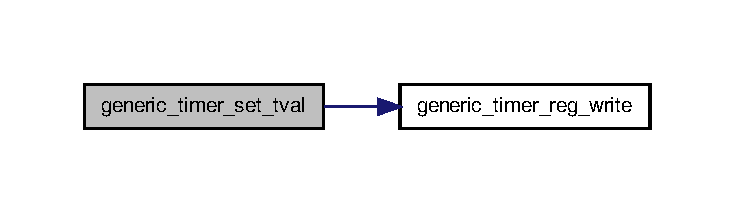
\includegraphics[width=350pt]{generic__timer_8c_a9c827fc2504de623842afa015a0791e2_cgraph}
\end{center}
\end{figure}




\subsection{\-Variable \-Documentation}
\hypertarget{generic__timer_8c_a793f595a9f49f888bb9f6a50fc960e93}{\index{generic\-\_\-timer.\-c@{generic\-\_\-timer.\-c}!\-\_\-callback@{\-\_\-callback}}
\index{\-\_\-callback@{\-\_\-callback}!generic_timer.c@{generic\-\_\-timer.\-c}}
\subsubsection[{\-\_\-callback}]{\setlength{\rightskip}{0pt plus 5cm}{\bf generic\-\_\-timer\-\_\-callback\-\_\-t} {\bf \-\_\-callback}\mbox{[}{\bf \-G\-E\-N\-E\-R\-I\-C\-\_\-\-T\-I\-M\-E\-R\-\_\-\-N\-U\-M\-\_\-\-T\-Y\-P\-E\-S}\mbox{]}\hspace{0.3cm}{\ttfamily  \mbox{[}static\mbox{]}}}}\label{generic__timer_8c_a793f595a9f49f888bb9f6a50fc960e93}


\-Definition at line 11 of file generic\-\_\-timer.\-c.

\hypertarget{generic__timer_8c_a5b94dd32413eab57ab72bb4b759fc703}{\index{generic\-\_\-timer.\-c@{generic\-\_\-timer.\-c}!\-\_\-timer\-\_\-irqs@{\-\_\-timer\-\_\-irqs}}
\index{\-\_\-timer\-\_\-irqs@{\-\_\-timer\-\_\-irqs}!generic_timer.c@{generic\-\_\-timer.\-c}}
\subsubsection[{\-\_\-timer\-\_\-irqs}]{\setlength{\rightskip}{0pt plus 5cm}{\bf uint32\-\_\-t} {\bf \-\_\-timer\-\_\-irqs}\mbox{[}{\bf \-G\-E\-N\-E\-R\-I\-C\-\_\-\-T\-I\-M\-E\-R\-\_\-\-N\-U\-M\-\_\-\-T\-Y\-P\-E\-S}\mbox{]}\hspace{0.3cm}{\ttfamily  \mbox{[}static\mbox{]}}}}\label{generic__timer_8c_a5b94dd32413eab57ab72bb4b759fc703}


\-Definition at line 9 of file generic\-\_\-timer.\-c.

\hypertarget{generic__timer_8c_a05bc27c00841323051dcd14eaf0d95c4}{\index{generic\-\_\-timer.\-c@{generic\-\_\-timer.\-c}!\-\_\-tvals@{\-\_\-tvals}}
\index{\-\_\-tvals@{\-\_\-tvals}!generic_timer.c@{generic\-\_\-timer.\-c}}
\subsubsection[{\-\_\-tvals}]{\setlength{\rightskip}{0pt plus 5cm}{\bf uint32\-\_\-t} {\bf \-\_\-tvals}\mbox{[}{\bf \-G\-E\-N\-E\-R\-I\-C\-\_\-\-T\-I\-M\-E\-R\-\_\-\-N\-U\-M\-\_\-\-T\-Y\-P\-E\-S}\mbox{]}\hspace{0.3cm}{\ttfamily  \mbox{[}static\mbox{]}}}}\label{generic__timer_8c_a05bc27c00841323051dcd14eaf0d95c4}


\-Definition at line 10 of file generic\-\_\-timer.\-c.


\hypertarget{generic__timer__regs_8h}{\section{generic\-\_\-timer/generic\-\_\-timer\-\_\-regs.h \-File \-Reference}
\label{generic__timer__regs_8h}\index{generic\-\_\-timer/generic\-\_\-timer\-\_\-regs.\-h@{generic\-\_\-timer/generic\-\_\-timer\-\_\-regs.\-h}}
}
{\ttfamily \#include \char`\"{}asm-\/arm\-\_\-inline.\-h\char`\"{}}\*
{\ttfamily \#include \char`\"{}armv7\-\_\-p15.\-h\char`\"{}}\*
{\ttfamily \#include \char`\"{}arch\-\_\-types.\-h\char`\"{}}\*
\-Include dependency graph for generic\-\_\-timer\-\_\-regs.\-h\-:
\nopagebreak
\begin{figure}[H]
\begin{center}
\leavevmode
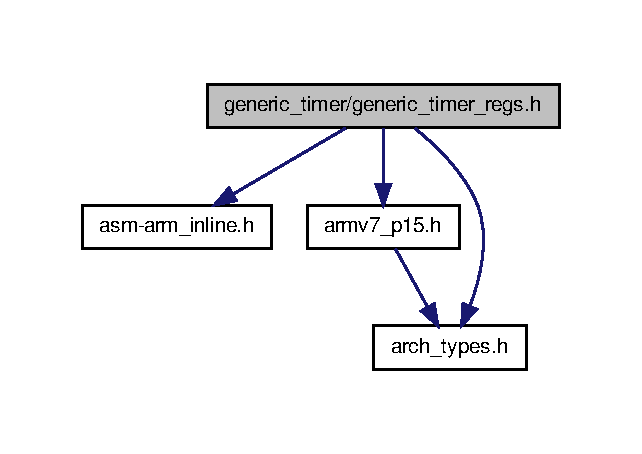
\includegraphics[width=308pt]{generic__timer__regs_8h__incl}
\end{center}
\end{figure}
\-This graph shows which files directly or indirectly include this file\-:
\nopagebreak
\begin{figure}[H]
\begin{center}
\leavevmode
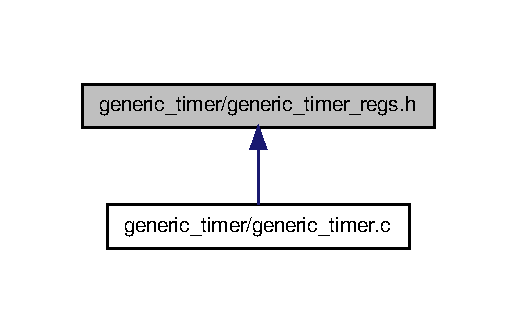
\includegraphics[width=248pt]{generic__timer__regs_8h__dep__incl}
\end{center}
\end{figure}
\subsection*{\-Defines}
\begin{DoxyCompactItemize}
\item 
\#define \hyperlink{generic__timer__regs_8h_a8efa8ea74c4e67832062909f9544354b}{\-G\-E\-N\-E\-R\-I\-C\-\_\-\-T\-I\-M\-E\-R\-\_\-\-C\-T\-R\-L\-\_\-\-E\-N\-A\-B\-L\-E}~(1 $<$$<$ 0)
\item 
\#define \hyperlink{generic__timer__regs_8h_a53e23d75a48e68fbf31a243d794fe2e7}{\-G\-E\-N\-E\-R\-I\-C\-\_\-\-T\-I\-M\-E\-R\-\_\-\-C\-T\-R\-L\-\_\-\-I\-M\-A\-S\-K}~(1 $<$$<$ 1)
\item 
\#define \hyperlink{generic__timer__regs_8h_ad603580a3a296a42124dc3ffb1616947}{\-G\-E\-N\-E\-R\-I\-C\-\_\-\-T\-I\-M\-E\-R\-\_\-\-C\-T\-R\-L\-\_\-\-I\-S\-T\-A\-T\-U\-S}~(1 $<$$<$ 2)
\item 
\#define \hyperlink{generic__timer__regs_8h_a45b1cfb471471ddbb3ea689a33f1e421}{generic\-\_\-timer\-\_\-pcounter\-\_\-read}()~\hyperlink{armv7__p15_8h_a4939c99e7b83a6fbef2867ab52240464}{read\-\_\-cntpct}()
\item 
\#define \hyperlink{generic__timer__regs_8h_a9655b66250137c8c6cf25bb82fd2c93a}{generic\-\_\-timer\-\_\-vcounter\-\_\-read}()~\hyperlink{armv7__p15_8h_a12e577d17891dc46fcc76e72f6bbd9f0}{read\-\_\-cntvct}()
\end{DoxyCompactItemize}
\subsection*{\-Enumerations}
\begin{DoxyCompactItemize}
\item 
enum \{ \*
\hyperlink{generic__timer__regs_8h_a06fc87d81c62e9abb8790b6e5713c55ba72361d9748f2b2954e2739c9533bceae}{\-G\-E\-N\-E\-R\-I\-C\-\_\-\-T\-I\-M\-E\-R\-\_\-\-R\-E\-G\-\_\-\-F\-R\-E\-Q}, 
\hyperlink{generic__timer__regs_8h_a06fc87d81c62e9abb8790b6e5713c55ba4bf0a7695baa4937c2f736806d9e0822}{\-G\-E\-N\-E\-R\-I\-C\-\_\-\-T\-I\-M\-E\-R\-\_\-\-R\-E\-G\-\_\-\-H\-C\-T\-L}, 
\hyperlink{generic__timer__regs_8h_a06fc87d81c62e9abb8790b6e5713c55ba625f655f0428421a5c4148fbdd2ea436}{\-G\-E\-N\-E\-R\-I\-C\-\_\-\-T\-I\-M\-E\-R\-\_\-\-R\-E\-G\-\_\-\-K\-C\-T\-L}, 
\hyperlink{generic__timer__regs_8h_a06fc87d81c62e9abb8790b6e5713c55bad25f4c8359d56a0e5ca6e71fc1f5c662}{\-G\-E\-N\-E\-R\-I\-C\-\_\-\-T\-I\-M\-E\-R\-\_\-\-R\-E\-G\-\_\-\-H\-Y\-P\-\_\-\-C\-T\-R\-L}, 
\*
\hyperlink{generic__timer__regs_8h_a06fc87d81c62e9abb8790b6e5713c55baa8cd51c8309bd3de48671c3c533f1e8e}{\-G\-E\-N\-E\-R\-I\-C\-\_\-\-T\-I\-M\-E\-R\-\_\-\-R\-E\-G\-\_\-\-H\-Y\-P\-\_\-\-T\-V\-A\-L}, 
\hyperlink{generic__timer__regs_8h_a06fc87d81c62e9abb8790b6e5713c55ba616c71960835bc93650409b53a198f11}{\-G\-E\-N\-E\-R\-I\-C\-\_\-\-T\-I\-M\-E\-R\-\_\-\-R\-E\-G\-\_\-\-H\-Y\-P\-\_\-\-C\-V\-A\-L}, 
\hyperlink{generic__timer__regs_8h_a06fc87d81c62e9abb8790b6e5713c55baccef1901d59fd32a320e10ff157cbda5}{\-G\-E\-N\-E\-R\-I\-C\-\_\-\-T\-I\-M\-E\-R\-\_\-\-R\-E\-G\-\_\-\-P\-H\-Y\-S\-\_\-\-C\-T\-R\-L}, 
\hyperlink{generic__timer__regs_8h_a06fc87d81c62e9abb8790b6e5713c55ba7d9f1f59c653f543a551dfd088a9a259}{\-G\-E\-N\-E\-R\-I\-C\-\_\-\-T\-I\-M\-E\-R\-\_\-\-R\-E\-G\-\_\-\-P\-H\-Y\-S\-\_\-\-T\-V\-A\-L}, 
\*
\hyperlink{generic__timer__regs_8h_a06fc87d81c62e9abb8790b6e5713c55bad3d982029e3a387108b36198ee893830}{\-G\-E\-N\-E\-R\-I\-C\-\_\-\-T\-I\-M\-E\-R\-\_\-\-R\-E\-G\-\_\-\-P\-H\-Y\-S\-\_\-\-C\-V\-A\-L}, 
\hyperlink{generic__timer__regs_8h_a06fc87d81c62e9abb8790b6e5713c55ba10b1c4d53803d1bd92e70d3940f8e465}{\-G\-E\-N\-E\-R\-I\-C\-\_\-\-T\-I\-M\-E\-R\-\_\-\-R\-E\-G\-\_\-\-V\-I\-R\-T\-\_\-\-C\-T\-R\-L}, 
\hyperlink{generic__timer__regs_8h_a06fc87d81c62e9abb8790b6e5713c55ba5c11a6c81f505837c3896fc8eb70ab3e}{\-G\-E\-N\-E\-R\-I\-C\-\_\-\-T\-I\-M\-E\-R\-\_\-\-R\-E\-G\-\_\-\-V\-I\-R\-T\-\_\-\-T\-V\-A\-L}, 
\hyperlink{generic__timer__regs_8h_a06fc87d81c62e9abb8790b6e5713c55bab2beec1a34fdfd20e01e519832c20256}{\-G\-E\-N\-E\-R\-I\-C\-\_\-\-T\-I\-M\-E\-R\-\_\-\-R\-E\-G\-\_\-\-V\-I\-R\-T\-\_\-\-C\-V\-A\-L}, 
\*
\hyperlink{generic__timer__regs_8h_a06fc87d81c62e9abb8790b6e5713c55ba8176032681a504ed9323bf517aa41054}{\-G\-E\-N\-E\-R\-I\-C\-\_\-\-T\-I\-M\-E\-R\-\_\-\-R\-E\-G\-\_\-\-V\-I\-R\-T\-\_\-\-O\-F\-F}
 \}
\end{DoxyCompactItemize}
\subsection*{\-Functions}
\begin{DoxyCompactItemize}
\item 
static void \hyperlink{generic__timer__regs_8h_a21908c6f55add221caf5e3de30fe8f77}{generic\-\_\-timer\-\_\-reg\-\_\-write} (int reg, \hyperlink{arch__types_8h_a435d1572bf3f880d55459d9805097f62}{uint32\-\_\-t} val)
\item 
static \hyperlink{arch__types_8h_a435d1572bf3f880d55459d9805097f62}{uint32\-\_\-t} \hyperlink{generic__timer__regs_8h_a076a2f37c8f342ce8d64fda8bf6cdc90}{generic\-\_\-timer\-\_\-reg\-\_\-read} (int reg)
\item 
static void \hyperlink{generic__timer__regs_8h_a531989be17f7397a7b42dbf29cacc6ff}{generic\-\_\-timer\-\_\-reg\-\_\-write64} (int reg, \hyperlink{arch__types_8h_aaa5d1cd013383c889537491c3cfd9aad}{uint64\-\_\-t} val)
\item 
static \hyperlink{arch__types_8h_aaa5d1cd013383c889537491c3cfd9aad}{uint64\-\_\-t} \hyperlink{generic__timer__regs_8h_ac82169092a24b779c0b745cfc5371f33}{generic\-\_\-timer\-\_\-reg\-\_\-read64} (int reg)
\end{DoxyCompactItemize}


\subsection{\-Define \-Documentation}
\hypertarget{generic__timer__regs_8h_a8efa8ea74c4e67832062909f9544354b}{\index{generic\-\_\-timer\-\_\-regs.\-h@{generic\-\_\-timer\-\_\-regs.\-h}!\-G\-E\-N\-E\-R\-I\-C\-\_\-\-T\-I\-M\-E\-R\-\_\-\-C\-T\-R\-L\-\_\-\-E\-N\-A\-B\-L\-E@{\-G\-E\-N\-E\-R\-I\-C\-\_\-\-T\-I\-M\-E\-R\-\_\-\-C\-T\-R\-L\-\_\-\-E\-N\-A\-B\-L\-E}}
\index{\-G\-E\-N\-E\-R\-I\-C\-\_\-\-T\-I\-M\-E\-R\-\_\-\-C\-T\-R\-L\-\_\-\-E\-N\-A\-B\-L\-E@{\-G\-E\-N\-E\-R\-I\-C\-\_\-\-T\-I\-M\-E\-R\-\_\-\-C\-T\-R\-L\-\_\-\-E\-N\-A\-B\-L\-E}!generic_timer_regs.h@{generic\-\_\-timer\-\_\-regs.\-h}}
\subsubsection[{\-G\-E\-N\-E\-R\-I\-C\-\_\-\-T\-I\-M\-E\-R\-\_\-\-C\-T\-R\-L\-\_\-\-E\-N\-A\-B\-L\-E}]{\setlength{\rightskip}{0pt plus 5cm}\#define {\bf \-G\-E\-N\-E\-R\-I\-C\-\_\-\-T\-I\-M\-E\-R\-\_\-\-C\-T\-R\-L\-\_\-\-E\-N\-A\-B\-L\-E}~(1 $<$$<$ 0)}}\label{generic__timer__regs_8h_a8efa8ea74c4e67832062909f9544354b}


\-Definition at line 7 of file generic\-\_\-timer\-\_\-regs.\-h.

\hypertarget{generic__timer__regs_8h_a53e23d75a48e68fbf31a243d794fe2e7}{\index{generic\-\_\-timer\-\_\-regs.\-h@{generic\-\_\-timer\-\_\-regs.\-h}!\-G\-E\-N\-E\-R\-I\-C\-\_\-\-T\-I\-M\-E\-R\-\_\-\-C\-T\-R\-L\-\_\-\-I\-M\-A\-S\-K@{\-G\-E\-N\-E\-R\-I\-C\-\_\-\-T\-I\-M\-E\-R\-\_\-\-C\-T\-R\-L\-\_\-\-I\-M\-A\-S\-K}}
\index{\-G\-E\-N\-E\-R\-I\-C\-\_\-\-T\-I\-M\-E\-R\-\_\-\-C\-T\-R\-L\-\_\-\-I\-M\-A\-S\-K@{\-G\-E\-N\-E\-R\-I\-C\-\_\-\-T\-I\-M\-E\-R\-\_\-\-C\-T\-R\-L\-\_\-\-I\-M\-A\-S\-K}!generic_timer_regs.h@{generic\-\_\-timer\-\_\-regs.\-h}}
\subsubsection[{\-G\-E\-N\-E\-R\-I\-C\-\_\-\-T\-I\-M\-E\-R\-\_\-\-C\-T\-R\-L\-\_\-\-I\-M\-A\-S\-K}]{\setlength{\rightskip}{0pt plus 5cm}\#define {\bf \-G\-E\-N\-E\-R\-I\-C\-\_\-\-T\-I\-M\-E\-R\-\_\-\-C\-T\-R\-L\-\_\-\-I\-M\-A\-S\-K}~(1 $<$$<$ 1)}}\label{generic__timer__regs_8h_a53e23d75a48e68fbf31a243d794fe2e7}


\-Definition at line 8 of file generic\-\_\-timer\-\_\-regs.\-h.

\hypertarget{generic__timer__regs_8h_ad603580a3a296a42124dc3ffb1616947}{\index{generic\-\_\-timer\-\_\-regs.\-h@{generic\-\_\-timer\-\_\-regs.\-h}!\-G\-E\-N\-E\-R\-I\-C\-\_\-\-T\-I\-M\-E\-R\-\_\-\-C\-T\-R\-L\-\_\-\-I\-S\-T\-A\-T\-U\-S@{\-G\-E\-N\-E\-R\-I\-C\-\_\-\-T\-I\-M\-E\-R\-\_\-\-C\-T\-R\-L\-\_\-\-I\-S\-T\-A\-T\-U\-S}}
\index{\-G\-E\-N\-E\-R\-I\-C\-\_\-\-T\-I\-M\-E\-R\-\_\-\-C\-T\-R\-L\-\_\-\-I\-S\-T\-A\-T\-U\-S@{\-G\-E\-N\-E\-R\-I\-C\-\_\-\-T\-I\-M\-E\-R\-\_\-\-C\-T\-R\-L\-\_\-\-I\-S\-T\-A\-T\-U\-S}!generic_timer_regs.h@{generic\-\_\-timer\-\_\-regs.\-h}}
\subsubsection[{\-G\-E\-N\-E\-R\-I\-C\-\_\-\-T\-I\-M\-E\-R\-\_\-\-C\-T\-R\-L\-\_\-\-I\-S\-T\-A\-T\-U\-S}]{\setlength{\rightskip}{0pt plus 5cm}\#define {\bf \-G\-E\-N\-E\-R\-I\-C\-\_\-\-T\-I\-M\-E\-R\-\_\-\-C\-T\-R\-L\-\_\-\-I\-S\-T\-A\-T\-U\-S}~(1 $<$$<$ 2)}}\label{generic__timer__regs_8h_ad603580a3a296a42124dc3ffb1616947}


\-Definition at line 9 of file generic\-\_\-timer\-\_\-regs.\-h.

\hypertarget{generic__timer__regs_8h_a45b1cfb471471ddbb3ea689a33f1e421}{\index{generic\-\_\-timer\-\_\-regs.\-h@{generic\-\_\-timer\-\_\-regs.\-h}!generic\-\_\-timer\-\_\-pcounter\-\_\-read@{generic\-\_\-timer\-\_\-pcounter\-\_\-read}}
\index{generic\-\_\-timer\-\_\-pcounter\-\_\-read@{generic\-\_\-timer\-\_\-pcounter\-\_\-read}!generic_timer_regs.h@{generic\-\_\-timer\-\_\-regs.\-h}}
\subsubsection[{generic\-\_\-timer\-\_\-pcounter\-\_\-read}]{\setlength{\rightskip}{0pt plus 5cm}\#define {\bf generic\-\_\-timer\-\_\-pcounter\-\_\-read}(
\begin{DoxyParamCaption}
{}
\end{DoxyParamCaption}
)~{\bf read\-\_\-cntpct}()}}\label{generic__timer__regs_8h_a45b1cfb471471ddbb3ea689a33f1e421}


\-Definition at line 10 of file generic\-\_\-timer\-\_\-regs.\-h.

\hypertarget{generic__timer__regs_8h_a9655b66250137c8c6cf25bb82fd2c93a}{\index{generic\-\_\-timer\-\_\-regs.\-h@{generic\-\_\-timer\-\_\-regs.\-h}!generic\-\_\-timer\-\_\-vcounter\-\_\-read@{generic\-\_\-timer\-\_\-vcounter\-\_\-read}}
\index{generic\-\_\-timer\-\_\-vcounter\-\_\-read@{generic\-\_\-timer\-\_\-vcounter\-\_\-read}!generic_timer_regs.h@{generic\-\_\-timer\-\_\-regs.\-h}}
\subsubsection[{generic\-\_\-timer\-\_\-vcounter\-\_\-read}]{\setlength{\rightskip}{0pt plus 5cm}\#define {\bf generic\-\_\-timer\-\_\-vcounter\-\_\-read}(
\begin{DoxyParamCaption}
{}
\end{DoxyParamCaption}
)~{\bf read\-\_\-cntvct}()}}\label{generic__timer__regs_8h_a9655b66250137c8c6cf25bb82fd2c93a}


\-Definition at line 11 of file generic\-\_\-timer\-\_\-regs.\-h.



\subsection{\-Enumeration \-Type \-Documentation}
\hypertarget{generic__timer__regs_8h_a06fc87d81c62e9abb8790b6e5713c55b}{\subsubsection[{anonymous enum}]{\setlength{\rightskip}{0pt plus 5cm}anonymous enum}}\label{generic__timer__regs_8h_a06fc87d81c62e9abb8790b6e5713c55b}
\begin{Desc}
\item[\-Enumerator\-: ]\par
\begin{description}
\index{\-G\-E\-N\-E\-R\-I\-C\-\_\-\-T\-I\-M\-E\-R\-\_\-\-R\-E\-G\-\_\-\-F\-R\-E\-Q@{\-G\-E\-N\-E\-R\-I\-C\-\_\-\-T\-I\-M\-E\-R\-\_\-\-R\-E\-G\-\_\-\-F\-R\-E\-Q}!generic\-\_\-timer\-\_\-regs.\-h@{generic\-\_\-timer\-\_\-regs.\-h}}\index{generic\-\_\-timer\-\_\-regs.\-h@{generic\-\_\-timer\-\_\-regs.\-h}!\-G\-E\-N\-E\-R\-I\-C\-\_\-\-T\-I\-M\-E\-R\-\_\-\-R\-E\-G\-\_\-\-F\-R\-E\-Q@{\-G\-E\-N\-E\-R\-I\-C\-\_\-\-T\-I\-M\-E\-R\-\_\-\-R\-E\-G\-\_\-\-F\-R\-E\-Q}}\item[{\em 
\hypertarget{generic__timer__regs_8h_a06fc87d81c62e9abb8790b6e5713c55ba72361d9748f2b2954e2739c9533bceae}{\-G\-E\-N\-E\-R\-I\-C\-\_\-\-T\-I\-M\-E\-R\-\_\-\-R\-E\-G\-\_\-\-F\-R\-E\-Q}\label{generic__timer__regs_8h_a06fc87d81c62e9abb8790b6e5713c55ba72361d9748f2b2954e2739c9533bceae}
}]\index{\-G\-E\-N\-E\-R\-I\-C\-\_\-\-T\-I\-M\-E\-R\-\_\-\-R\-E\-G\-\_\-\-H\-C\-T\-L@{\-G\-E\-N\-E\-R\-I\-C\-\_\-\-T\-I\-M\-E\-R\-\_\-\-R\-E\-G\-\_\-\-H\-C\-T\-L}!generic\-\_\-timer\-\_\-regs.\-h@{generic\-\_\-timer\-\_\-regs.\-h}}\index{generic\-\_\-timer\-\_\-regs.\-h@{generic\-\_\-timer\-\_\-regs.\-h}!\-G\-E\-N\-E\-R\-I\-C\-\_\-\-T\-I\-M\-E\-R\-\_\-\-R\-E\-G\-\_\-\-H\-C\-T\-L@{\-G\-E\-N\-E\-R\-I\-C\-\_\-\-T\-I\-M\-E\-R\-\_\-\-R\-E\-G\-\_\-\-H\-C\-T\-L}}\item[{\em 
\hypertarget{generic__timer__regs_8h_a06fc87d81c62e9abb8790b6e5713c55ba4bf0a7695baa4937c2f736806d9e0822}{\-G\-E\-N\-E\-R\-I\-C\-\_\-\-T\-I\-M\-E\-R\-\_\-\-R\-E\-G\-\_\-\-H\-C\-T\-L}\label{generic__timer__regs_8h_a06fc87d81c62e9abb8790b6e5713c55ba4bf0a7695baa4937c2f736806d9e0822}
}]\index{\-G\-E\-N\-E\-R\-I\-C\-\_\-\-T\-I\-M\-E\-R\-\_\-\-R\-E\-G\-\_\-\-K\-C\-T\-L@{\-G\-E\-N\-E\-R\-I\-C\-\_\-\-T\-I\-M\-E\-R\-\_\-\-R\-E\-G\-\_\-\-K\-C\-T\-L}!generic\-\_\-timer\-\_\-regs.\-h@{generic\-\_\-timer\-\_\-regs.\-h}}\index{generic\-\_\-timer\-\_\-regs.\-h@{generic\-\_\-timer\-\_\-regs.\-h}!\-G\-E\-N\-E\-R\-I\-C\-\_\-\-T\-I\-M\-E\-R\-\_\-\-R\-E\-G\-\_\-\-K\-C\-T\-L@{\-G\-E\-N\-E\-R\-I\-C\-\_\-\-T\-I\-M\-E\-R\-\_\-\-R\-E\-G\-\_\-\-K\-C\-T\-L}}\item[{\em 
\hypertarget{generic__timer__regs_8h_a06fc87d81c62e9abb8790b6e5713c55ba625f655f0428421a5c4148fbdd2ea436}{\-G\-E\-N\-E\-R\-I\-C\-\_\-\-T\-I\-M\-E\-R\-\_\-\-R\-E\-G\-\_\-\-K\-C\-T\-L}\label{generic__timer__regs_8h_a06fc87d81c62e9abb8790b6e5713c55ba625f655f0428421a5c4148fbdd2ea436}
}]\index{\-G\-E\-N\-E\-R\-I\-C\-\_\-\-T\-I\-M\-E\-R\-\_\-\-R\-E\-G\-\_\-\-H\-Y\-P\-\_\-\-C\-T\-R\-L@{\-G\-E\-N\-E\-R\-I\-C\-\_\-\-T\-I\-M\-E\-R\-\_\-\-R\-E\-G\-\_\-\-H\-Y\-P\-\_\-\-C\-T\-R\-L}!generic\-\_\-timer\-\_\-regs.\-h@{generic\-\_\-timer\-\_\-regs.\-h}}\index{generic\-\_\-timer\-\_\-regs.\-h@{generic\-\_\-timer\-\_\-regs.\-h}!\-G\-E\-N\-E\-R\-I\-C\-\_\-\-T\-I\-M\-E\-R\-\_\-\-R\-E\-G\-\_\-\-H\-Y\-P\-\_\-\-C\-T\-R\-L@{\-G\-E\-N\-E\-R\-I\-C\-\_\-\-T\-I\-M\-E\-R\-\_\-\-R\-E\-G\-\_\-\-H\-Y\-P\-\_\-\-C\-T\-R\-L}}\item[{\em 
\hypertarget{generic__timer__regs_8h_a06fc87d81c62e9abb8790b6e5713c55bad25f4c8359d56a0e5ca6e71fc1f5c662}{\-G\-E\-N\-E\-R\-I\-C\-\_\-\-T\-I\-M\-E\-R\-\_\-\-R\-E\-G\-\_\-\-H\-Y\-P\-\_\-\-C\-T\-R\-L}\label{generic__timer__regs_8h_a06fc87d81c62e9abb8790b6e5713c55bad25f4c8359d56a0e5ca6e71fc1f5c662}
}]\index{\-G\-E\-N\-E\-R\-I\-C\-\_\-\-T\-I\-M\-E\-R\-\_\-\-R\-E\-G\-\_\-\-H\-Y\-P\-\_\-\-T\-V\-A\-L@{\-G\-E\-N\-E\-R\-I\-C\-\_\-\-T\-I\-M\-E\-R\-\_\-\-R\-E\-G\-\_\-\-H\-Y\-P\-\_\-\-T\-V\-A\-L}!generic\-\_\-timer\-\_\-regs.\-h@{generic\-\_\-timer\-\_\-regs.\-h}}\index{generic\-\_\-timer\-\_\-regs.\-h@{generic\-\_\-timer\-\_\-regs.\-h}!\-G\-E\-N\-E\-R\-I\-C\-\_\-\-T\-I\-M\-E\-R\-\_\-\-R\-E\-G\-\_\-\-H\-Y\-P\-\_\-\-T\-V\-A\-L@{\-G\-E\-N\-E\-R\-I\-C\-\_\-\-T\-I\-M\-E\-R\-\_\-\-R\-E\-G\-\_\-\-H\-Y\-P\-\_\-\-T\-V\-A\-L}}\item[{\em 
\hypertarget{generic__timer__regs_8h_a06fc87d81c62e9abb8790b6e5713c55baa8cd51c8309bd3de48671c3c533f1e8e}{\-G\-E\-N\-E\-R\-I\-C\-\_\-\-T\-I\-M\-E\-R\-\_\-\-R\-E\-G\-\_\-\-H\-Y\-P\-\_\-\-T\-V\-A\-L}\label{generic__timer__regs_8h_a06fc87d81c62e9abb8790b6e5713c55baa8cd51c8309bd3de48671c3c533f1e8e}
}]\index{\-G\-E\-N\-E\-R\-I\-C\-\_\-\-T\-I\-M\-E\-R\-\_\-\-R\-E\-G\-\_\-\-H\-Y\-P\-\_\-\-C\-V\-A\-L@{\-G\-E\-N\-E\-R\-I\-C\-\_\-\-T\-I\-M\-E\-R\-\_\-\-R\-E\-G\-\_\-\-H\-Y\-P\-\_\-\-C\-V\-A\-L}!generic\-\_\-timer\-\_\-regs.\-h@{generic\-\_\-timer\-\_\-regs.\-h}}\index{generic\-\_\-timer\-\_\-regs.\-h@{generic\-\_\-timer\-\_\-regs.\-h}!\-G\-E\-N\-E\-R\-I\-C\-\_\-\-T\-I\-M\-E\-R\-\_\-\-R\-E\-G\-\_\-\-H\-Y\-P\-\_\-\-C\-V\-A\-L@{\-G\-E\-N\-E\-R\-I\-C\-\_\-\-T\-I\-M\-E\-R\-\_\-\-R\-E\-G\-\_\-\-H\-Y\-P\-\_\-\-C\-V\-A\-L}}\item[{\em 
\hypertarget{generic__timer__regs_8h_a06fc87d81c62e9abb8790b6e5713c55ba616c71960835bc93650409b53a198f11}{\-G\-E\-N\-E\-R\-I\-C\-\_\-\-T\-I\-M\-E\-R\-\_\-\-R\-E\-G\-\_\-\-H\-Y\-P\-\_\-\-C\-V\-A\-L}\label{generic__timer__regs_8h_a06fc87d81c62e9abb8790b6e5713c55ba616c71960835bc93650409b53a198f11}
}]\index{\-G\-E\-N\-E\-R\-I\-C\-\_\-\-T\-I\-M\-E\-R\-\_\-\-R\-E\-G\-\_\-\-P\-H\-Y\-S\-\_\-\-C\-T\-R\-L@{\-G\-E\-N\-E\-R\-I\-C\-\_\-\-T\-I\-M\-E\-R\-\_\-\-R\-E\-G\-\_\-\-P\-H\-Y\-S\-\_\-\-C\-T\-R\-L}!generic\-\_\-timer\-\_\-regs.\-h@{generic\-\_\-timer\-\_\-regs.\-h}}\index{generic\-\_\-timer\-\_\-regs.\-h@{generic\-\_\-timer\-\_\-regs.\-h}!\-G\-E\-N\-E\-R\-I\-C\-\_\-\-T\-I\-M\-E\-R\-\_\-\-R\-E\-G\-\_\-\-P\-H\-Y\-S\-\_\-\-C\-T\-R\-L@{\-G\-E\-N\-E\-R\-I\-C\-\_\-\-T\-I\-M\-E\-R\-\_\-\-R\-E\-G\-\_\-\-P\-H\-Y\-S\-\_\-\-C\-T\-R\-L}}\item[{\em 
\hypertarget{generic__timer__regs_8h_a06fc87d81c62e9abb8790b6e5713c55baccef1901d59fd32a320e10ff157cbda5}{\-G\-E\-N\-E\-R\-I\-C\-\_\-\-T\-I\-M\-E\-R\-\_\-\-R\-E\-G\-\_\-\-P\-H\-Y\-S\-\_\-\-C\-T\-R\-L}\label{generic__timer__regs_8h_a06fc87d81c62e9abb8790b6e5713c55baccef1901d59fd32a320e10ff157cbda5}
}]\index{\-G\-E\-N\-E\-R\-I\-C\-\_\-\-T\-I\-M\-E\-R\-\_\-\-R\-E\-G\-\_\-\-P\-H\-Y\-S\-\_\-\-T\-V\-A\-L@{\-G\-E\-N\-E\-R\-I\-C\-\_\-\-T\-I\-M\-E\-R\-\_\-\-R\-E\-G\-\_\-\-P\-H\-Y\-S\-\_\-\-T\-V\-A\-L}!generic\-\_\-timer\-\_\-regs.\-h@{generic\-\_\-timer\-\_\-regs.\-h}}\index{generic\-\_\-timer\-\_\-regs.\-h@{generic\-\_\-timer\-\_\-regs.\-h}!\-G\-E\-N\-E\-R\-I\-C\-\_\-\-T\-I\-M\-E\-R\-\_\-\-R\-E\-G\-\_\-\-P\-H\-Y\-S\-\_\-\-T\-V\-A\-L@{\-G\-E\-N\-E\-R\-I\-C\-\_\-\-T\-I\-M\-E\-R\-\_\-\-R\-E\-G\-\_\-\-P\-H\-Y\-S\-\_\-\-T\-V\-A\-L}}\item[{\em 
\hypertarget{generic__timer__regs_8h_a06fc87d81c62e9abb8790b6e5713c55ba7d9f1f59c653f543a551dfd088a9a259}{\-G\-E\-N\-E\-R\-I\-C\-\_\-\-T\-I\-M\-E\-R\-\_\-\-R\-E\-G\-\_\-\-P\-H\-Y\-S\-\_\-\-T\-V\-A\-L}\label{generic__timer__regs_8h_a06fc87d81c62e9abb8790b6e5713c55ba7d9f1f59c653f543a551dfd088a9a259}
}]\index{\-G\-E\-N\-E\-R\-I\-C\-\_\-\-T\-I\-M\-E\-R\-\_\-\-R\-E\-G\-\_\-\-P\-H\-Y\-S\-\_\-\-C\-V\-A\-L@{\-G\-E\-N\-E\-R\-I\-C\-\_\-\-T\-I\-M\-E\-R\-\_\-\-R\-E\-G\-\_\-\-P\-H\-Y\-S\-\_\-\-C\-V\-A\-L}!generic\-\_\-timer\-\_\-regs.\-h@{generic\-\_\-timer\-\_\-regs.\-h}}\index{generic\-\_\-timer\-\_\-regs.\-h@{generic\-\_\-timer\-\_\-regs.\-h}!\-G\-E\-N\-E\-R\-I\-C\-\_\-\-T\-I\-M\-E\-R\-\_\-\-R\-E\-G\-\_\-\-P\-H\-Y\-S\-\_\-\-C\-V\-A\-L@{\-G\-E\-N\-E\-R\-I\-C\-\_\-\-T\-I\-M\-E\-R\-\_\-\-R\-E\-G\-\_\-\-P\-H\-Y\-S\-\_\-\-C\-V\-A\-L}}\item[{\em 
\hypertarget{generic__timer__regs_8h_a06fc87d81c62e9abb8790b6e5713c55bad3d982029e3a387108b36198ee893830}{\-G\-E\-N\-E\-R\-I\-C\-\_\-\-T\-I\-M\-E\-R\-\_\-\-R\-E\-G\-\_\-\-P\-H\-Y\-S\-\_\-\-C\-V\-A\-L}\label{generic__timer__regs_8h_a06fc87d81c62e9abb8790b6e5713c55bad3d982029e3a387108b36198ee893830}
}]\index{\-G\-E\-N\-E\-R\-I\-C\-\_\-\-T\-I\-M\-E\-R\-\_\-\-R\-E\-G\-\_\-\-V\-I\-R\-T\-\_\-\-C\-T\-R\-L@{\-G\-E\-N\-E\-R\-I\-C\-\_\-\-T\-I\-M\-E\-R\-\_\-\-R\-E\-G\-\_\-\-V\-I\-R\-T\-\_\-\-C\-T\-R\-L}!generic\-\_\-timer\-\_\-regs.\-h@{generic\-\_\-timer\-\_\-regs.\-h}}\index{generic\-\_\-timer\-\_\-regs.\-h@{generic\-\_\-timer\-\_\-regs.\-h}!\-G\-E\-N\-E\-R\-I\-C\-\_\-\-T\-I\-M\-E\-R\-\_\-\-R\-E\-G\-\_\-\-V\-I\-R\-T\-\_\-\-C\-T\-R\-L@{\-G\-E\-N\-E\-R\-I\-C\-\_\-\-T\-I\-M\-E\-R\-\_\-\-R\-E\-G\-\_\-\-V\-I\-R\-T\-\_\-\-C\-T\-R\-L}}\item[{\em 
\hypertarget{generic__timer__regs_8h_a06fc87d81c62e9abb8790b6e5713c55ba10b1c4d53803d1bd92e70d3940f8e465}{\-G\-E\-N\-E\-R\-I\-C\-\_\-\-T\-I\-M\-E\-R\-\_\-\-R\-E\-G\-\_\-\-V\-I\-R\-T\-\_\-\-C\-T\-R\-L}\label{generic__timer__regs_8h_a06fc87d81c62e9abb8790b6e5713c55ba10b1c4d53803d1bd92e70d3940f8e465}
}]\index{\-G\-E\-N\-E\-R\-I\-C\-\_\-\-T\-I\-M\-E\-R\-\_\-\-R\-E\-G\-\_\-\-V\-I\-R\-T\-\_\-\-T\-V\-A\-L@{\-G\-E\-N\-E\-R\-I\-C\-\_\-\-T\-I\-M\-E\-R\-\_\-\-R\-E\-G\-\_\-\-V\-I\-R\-T\-\_\-\-T\-V\-A\-L}!generic\-\_\-timer\-\_\-regs.\-h@{generic\-\_\-timer\-\_\-regs.\-h}}\index{generic\-\_\-timer\-\_\-regs.\-h@{generic\-\_\-timer\-\_\-regs.\-h}!\-G\-E\-N\-E\-R\-I\-C\-\_\-\-T\-I\-M\-E\-R\-\_\-\-R\-E\-G\-\_\-\-V\-I\-R\-T\-\_\-\-T\-V\-A\-L@{\-G\-E\-N\-E\-R\-I\-C\-\_\-\-T\-I\-M\-E\-R\-\_\-\-R\-E\-G\-\_\-\-V\-I\-R\-T\-\_\-\-T\-V\-A\-L}}\item[{\em 
\hypertarget{generic__timer__regs_8h_a06fc87d81c62e9abb8790b6e5713c55ba5c11a6c81f505837c3896fc8eb70ab3e}{\-G\-E\-N\-E\-R\-I\-C\-\_\-\-T\-I\-M\-E\-R\-\_\-\-R\-E\-G\-\_\-\-V\-I\-R\-T\-\_\-\-T\-V\-A\-L}\label{generic__timer__regs_8h_a06fc87d81c62e9abb8790b6e5713c55ba5c11a6c81f505837c3896fc8eb70ab3e}
}]\index{\-G\-E\-N\-E\-R\-I\-C\-\_\-\-T\-I\-M\-E\-R\-\_\-\-R\-E\-G\-\_\-\-V\-I\-R\-T\-\_\-\-C\-V\-A\-L@{\-G\-E\-N\-E\-R\-I\-C\-\_\-\-T\-I\-M\-E\-R\-\_\-\-R\-E\-G\-\_\-\-V\-I\-R\-T\-\_\-\-C\-V\-A\-L}!generic\-\_\-timer\-\_\-regs.\-h@{generic\-\_\-timer\-\_\-regs.\-h}}\index{generic\-\_\-timer\-\_\-regs.\-h@{generic\-\_\-timer\-\_\-regs.\-h}!\-G\-E\-N\-E\-R\-I\-C\-\_\-\-T\-I\-M\-E\-R\-\_\-\-R\-E\-G\-\_\-\-V\-I\-R\-T\-\_\-\-C\-V\-A\-L@{\-G\-E\-N\-E\-R\-I\-C\-\_\-\-T\-I\-M\-E\-R\-\_\-\-R\-E\-G\-\_\-\-V\-I\-R\-T\-\_\-\-C\-V\-A\-L}}\item[{\em 
\hypertarget{generic__timer__regs_8h_a06fc87d81c62e9abb8790b6e5713c55bab2beec1a34fdfd20e01e519832c20256}{\-G\-E\-N\-E\-R\-I\-C\-\_\-\-T\-I\-M\-E\-R\-\_\-\-R\-E\-G\-\_\-\-V\-I\-R\-T\-\_\-\-C\-V\-A\-L}\label{generic__timer__regs_8h_a06fc87d81c62e9abb8790b6e5713c55bab2beec1a34fdfd20e01e519832c20256}
}]\index{\-G\-E\-N\-E\-R\-I\-C\-\_\-\-T\-I\-M\-E\-R\-\_\-\-R\-E\-G\-\_\-\-V\-I\-R\-T\-\_\-\-O\-F\-F@{\-G\-E\-N\-E\-R\-I\-C\-\_\-\-T\-I\-M\-E\-R\-\_\-\-R\-E\-G\-\_\-\-V\-I\-R\-T\-\_\-\-O\-F\-F}!generic\-\_\-timer\-\_\-regs.\-h@{generic\-\_\-timer\-\_\-regs.\-h}}\index{generic\-\_\-timer\-\_\-regs.\-h@{generic\-\_\-timer\-\_\-regs.\-h}!\-G\-E\-N\-E\-R\-I\-C\-\_\-\-T\-I\-M\-E\-R\-\_\-\-R\-E\-G\-\_\-\-V\-I\-R\-T\-\_\-\-O\-F\-F@{\-G\-E\-N\-E\-R\-I\-C\-\_\-\-T\-I\-M\-E\-R\-\_\-\-R\-E\-G\-\_\-\-V\-I\-R\-T\-\_\-\-O\-F\-F}}\item[{\em 
\hypertarget{generic__timer__regs_8h_a06fc87d81c62e9abb8790b6e5713c55ba8176032681a504ed9323bf517aa41054}{\-G\-E\-N\-E\-R\-I\-C\-\_\-\-T\-I\-M\-E\-R\-\_\-\-R\-E\-G\-\_\-\-V\-I\-R\-T\-\_\-\-O\-F\-F}\label{generic__timer__regs_8h_a06fc87d81c62e9abb8790b6e5713c55ba8176032681a504ed9323bf517aa41054}
}]\end{description}
\end{Desc}



\-Definition at line 14 of file generic\-\_\-timer\-\_\-regs.\-h.


\begin{DoxyCode}
     {
    GENERIC_TIMER_REG_FREQ,
    GENERIC_TIMER_REG_HCTL,
    GENERIC_TIMER_REG_KCTL,
    GENERIC_TIMER_REG_HYP_CTRL,
    GENERIC_TIMER_REG_HYP_TVAL,
    GENERIC_TIMER_REG_HYP_CVAL,
    GENERIC_TIMER_REG_PHYS_CTRL,
    GENERIC_TIMER_REG_PHYS_TVAL,
    GENERIC_TIMER_REG_PHYS_CVAL,
    GENERIC_TIMER_REG_VIRT_CTRL,
    GENERIC_TIMER_REG_VIRT_TVAL,
    GENERIC_TIMER_REG_VIRT_CVAL,
    GENERIC_TIMER_REG_VIRT_OFF,
};
\end{DoxyCode}


\subsection{\-Function \-Documentation}
\hypertarget{generic__timer__regs_8h_a076a2f37c8f342ce8d64fda8bf6cdc90}{\index{generic\-\_\-timer\-\_\-regs.\-h@{generic\-\_\-timer\-\_\-regs.\-h}!generic\-\_\-timer\-\_\-reg\-\_\-read@{generic\-\_\-timer\-\_\-reg\-\_\-read}}
\index{generic\-\_\-timer\-\_\-reg\-\_\-read@{generic\-\_\-timer\-\_\-reg\-\_\-read}!generic_timer_regs.h@{generic\-\_\-timer\-\_\-regs.\-h}}
\subsubsection[{generic\-\_\-timer\-\_\-reg\-\_\-read}]{\setlength{\rightskip}{0pt plus 5cm}static {\bf uint32\-\_\-t} {\bf generic\-\_\-timer\-\_\-reg\-\_\-read} (
\begin{DoxyParamCaption}
\item[{int}]{reg}
\end{DoxyParamCaption}
)\hspace{0.3cm}{\ttfamily  \mbox{[}inline, static\mbox{]}}}}\label{generic__timer__regs_8h_a076a2f37c8f342ce8d64fda8bf6cdc90}


\-Definition at line 68 of file generic\-\_\-timer\-\_\-regs.\-h.


\begin{DoxyCode}
{
    uint32_t val;

    switch (reg) {
    case GENERIC_TIMER_REG_FREQ:
        val = read_cntfrq();
        break;
    case GENERIC_TIMER_REG_HCTL:
        val = read_cnthctl();
        break;
    case GENERIC_TIMER_REG_KCTL:
        val = read_cntkctl();
        break;
    case GENERIC_TIMER_REG_HYP_CTRL:
        val = read_cnthp_ctl();
        break;
    case GENERIC_TIMER_REG_HYP_TVAL:
        val = read_cnthp_tval();
        break;
    case GENERIC_TIMER_REG_PHYS_CTRL:
        val = read_cntp_ctl();
        break;
    case GENERIC_TIMER_REG_PHYS_TVAL:
        val = read_cntp_tval();
        break;
    case GENERIC_TIMER_REG_VIRT_CTRL:
        val = read_cntv_ctl();
        break;
    case GENERIC_TIMER_REG_VIRT_TVAL:
        val = read_cntv_tval();
        break;
    default:
        uart_print("Trying to read invalid generic-timer register\n\r");
        break;
    }

    return val;
}
\end{DoxyCode}
\hypertarget{generic__timer__regs_8h_ac82169092a24b779c0b745cfc5371f33}{\index{generic\-\_\-timer\-\_\-regs.\-h@{generic\-\_\-timer\-\_\-regs.\-h}!generic\-\_\-timer\-\_\-reg\-\_\-read64@{generic\-\_\-timer\-\_\-reg\-\_\-read64}}
\index{generic\-\_\-timer\-\_\-reg\-\_\-read64@{generic\-\_\-timer\-\_\-reg\-\_\-read64}!generic_timer_regs.h@{generic\-\_\-timer\-\_\-regs.\-h}}
\subsubsection[{generic\-\_\-timer\-\_\-reg\-\_\-read64}]{\setlength{\rightskip}{0pt plus 5cm}static {\bf uint64\-\_\-t} {\bf generic\-\_\-timer\-\_\-reg\-\_\-read64} (
\begin{DoxyParamCaption}
\item[{int}]{reg}
\end{DoxyParamCaption}
)\hspace{0.3cm}{\ttfamily  \mbox{[}inline, static\mbox{]}}}}\label{generic__timer__regs_8h_ac82169092a24b779c0b745cfc5371f33}


\-Definition at line 131 of file generic\-\_\-timer\-\_\-regs.\-h.


\begin{DoxyCode}
{
    uint64_t val;

    switch (reg) {
    case GENERIC_TIMER_REG_HYP_CVAL:
        val = read_cnthp_cval();
        break;
    case GENERIC_TIMER_REG_PHYS_CVAL:
        val = read_cntp_tval();
        break;
    case GENERIC_TIMER_REG_VIRT_CVAL:
        val = read_cntv_cval();
        break;
    case GENERIC_TIMER_REG_VIRT_OFF:
        val = read_cntvoff();
        break;
    default:
        uart_print("Trying to read invalid generic-timer register\n\r");
        break;
    }

    return val;
}
\end{DoxyCode}
\hypertarget{generic__timer__regs_8h_a21908c6f55add221caf5e3de30fe8f77}{\index{generic\-\_\-timer\-\_\-regs.\-h@{generic\-\_\-timer\-\_\-regs.\-h}!generic\-\_\-timer\-\_\-reg\-\_\-write@{generic\-\_\-timer\-\_\-reg\-\_\-write}}
\index{generic\-\_\-timer\-\_\-reg\-\_\-write@{generic\-\_\-timer\-\_\-reg\-\_\-write}!generic_timer_regs.h@{generic\-\_\-timer\-\_\-regs.\-h}}
\subsubsection[{generic\-\_\-timer\-\_\-reg\-\_\-write}]{\setlength{\rightskip}{0pt plus 5cm}static void {\bf generic\-\_\-timer\-\_\-reg\-\_\-write} (
\begin{DoxyParamCaption}
\item[{int}]{reg, }
\item[{{\bf uint32\-\_\-t}}]{val}
\end{DoxyParamCaption}
)\hspace{0.3cm}{\ttfamily  \mbox{[}inline, static\mbox{]}}}}\label{generic__timer__regs_8h_a21908c6f55add221caf5e3de30fe8f77}


\-Definition at line 30 of file generic\-\_\-timer\-\_\-regs.\-h.


\begin{DoxyCode}
{
    switch (reg) {
    case GENERIC_TIMER_REG_FREQ:
        write_cntfrq(val);
        break;
    case GENERIC_TIMER_REG_HCTL:
        write_cnthctl(val);
        break;
    case GENERIC_TIMER_REG_KCTL:
        write_cntkctl(val);
        break;
    case GENERIC_TIMER_REG_HYP_CTRL:
        write_cnthp_ctl(val);
        break;
    case GENERIC_TIMER_REG_HYP_TVAL:
        write_cnthp_tval(val);
        break;
    case GENERIC_TIMER_REG_PHYS_CTRL:
        write_cntp_ctl(val);
        break;
    case GENERIC_TIMER_REG_PHYS_TVAL:
        write_cntp_tval(val);
        break;
    case GENERIC_TIMER_REG_VIRT_CTRL:
        write_cntv_ctl(val);
        break;
    case GENERIC_TIMER_REG_VIRT_TVAL:
        write_cntv_tval(val);
        break;
    default:
        uart_print("Trying to write invalid generic-timer register\n\r");
        break;
    }

    isb();
}
\end{DoxyCode}
\hypertarget{generic__timer__regs_8h_a531989be17f7397a7b42dbf29cacc6ff}{\index{generic\-\_\-timer\-\_\-regs.\-h@{generic\-\_\-timer\-\_\-regs.\-h}!generic\-\_\-timer\-\_\-reg\-\_\-write64@{generic\-\_\-timer\-\_\-reg\-\_\-write64}}
\index{generic\-\_\-timer\-\_\-reg\-\_\-write64@{generic\-\_\-timer\-\_\-reg\-\_\-write64}!generic_timer_regs.h@{generic\-\_\-timer\-\_\-regs.\-h}}
\subsubsection[{generic\-\_\-timer\-\_\-reg\-\_\-write64}]{\setlength{\rightskip}{0pt plus 5cm}static void {\bf generic\-\_\-timer\-\_\-reg\-\_\-write64} (
\begin{DoxyParamCaption}
\item[{int}]{reg, }
\item[{{\bf uint64\-\_\-t}}]{val}
\end{DoxyParamCaption}
)\hspace{0.3cm}{\ttfamily  \mbox{[}inline, static\mbox{]}}}}\label{generic__timer__regs_8h_a531989be17f7397a7b42dbf29cacc6ff}


\-Definition at line 108 of file generic\-\_\-timer\-\_\-regs.\-h.


\begin{DoxyCode}
{
    switch (reg) {
    case GENERIC_TIMER_REG_HYP_CVAL:
        write_cnthp_cval(val);
        break;
    case GENERIC_TIMER_REG_PHYS_CVAL:
        write_cntp_cval(val);
        break;
    case GENERIC_TIMER_REG_VIRT_CVAL:
        write_cntv_cval(val);
        break;
    case GENERIC_TIMER_REG_VIRT_OFF:
        write_cntvoff(val);
        break;
    default:
        uart_print("Trying to write invalid generic-timer register\n\r");
        break;
    }

    isb();
}
\end{DoxyCode}

\hypertarget{gic_8c}{\section{gic/gic.c \-File \-Reference}
\label{gic_8c}\index{gic/gic.\-c@{gic/gic.\-c}}
}
{\ttfamily \#include \char`\"{}gic.\-h\char`\"{}}\*
{\ttfamily \#include \char`\"{}armv7\-\_\-p15.\-h\char`\"{}}\*
{\ttfamily \#include \char`\"{}a15\-\_\-cp15\-\_\-sysregs.\-h\char`\"{}}\*
{\ttfamily \#include \char`\"{}smp.\-h\char`\"{}}\*
{\ttfamily \#include \char`\"{}context.\-h\char`\"{}}\*
{\ttfamily \#include \char`\"{}hvmm\-\_\-trace.\-h\char`\"{}}\*
{\ttfamily \#include $<$gic\-\_\-regs.\-h$>$}\*
{\ttfamily \#include \char`\"{}virqmap.\-h\char`\"{}}\*
{\ttfamily \#include \char`\"{}virq.\-h\char`\"{}}\*
{\ttfamily \#include \char`\"{}hvmm\-\_\-types.\-h\char`\"{}}\*
{\ttfamily \#include $<$log/print.\-h$>$}\*
{\ttfamily \#include $<$log/uart\-\_\-print.\-h$>$}\*
{\ttfamily \#include $<$config/cfg\-\_\-platform.\-h$>$}\*
\-Include dependency graph for gic.\-c\-:
\nopagebreak
\begin{figure}[H]
\begin{center}
\leavevmode
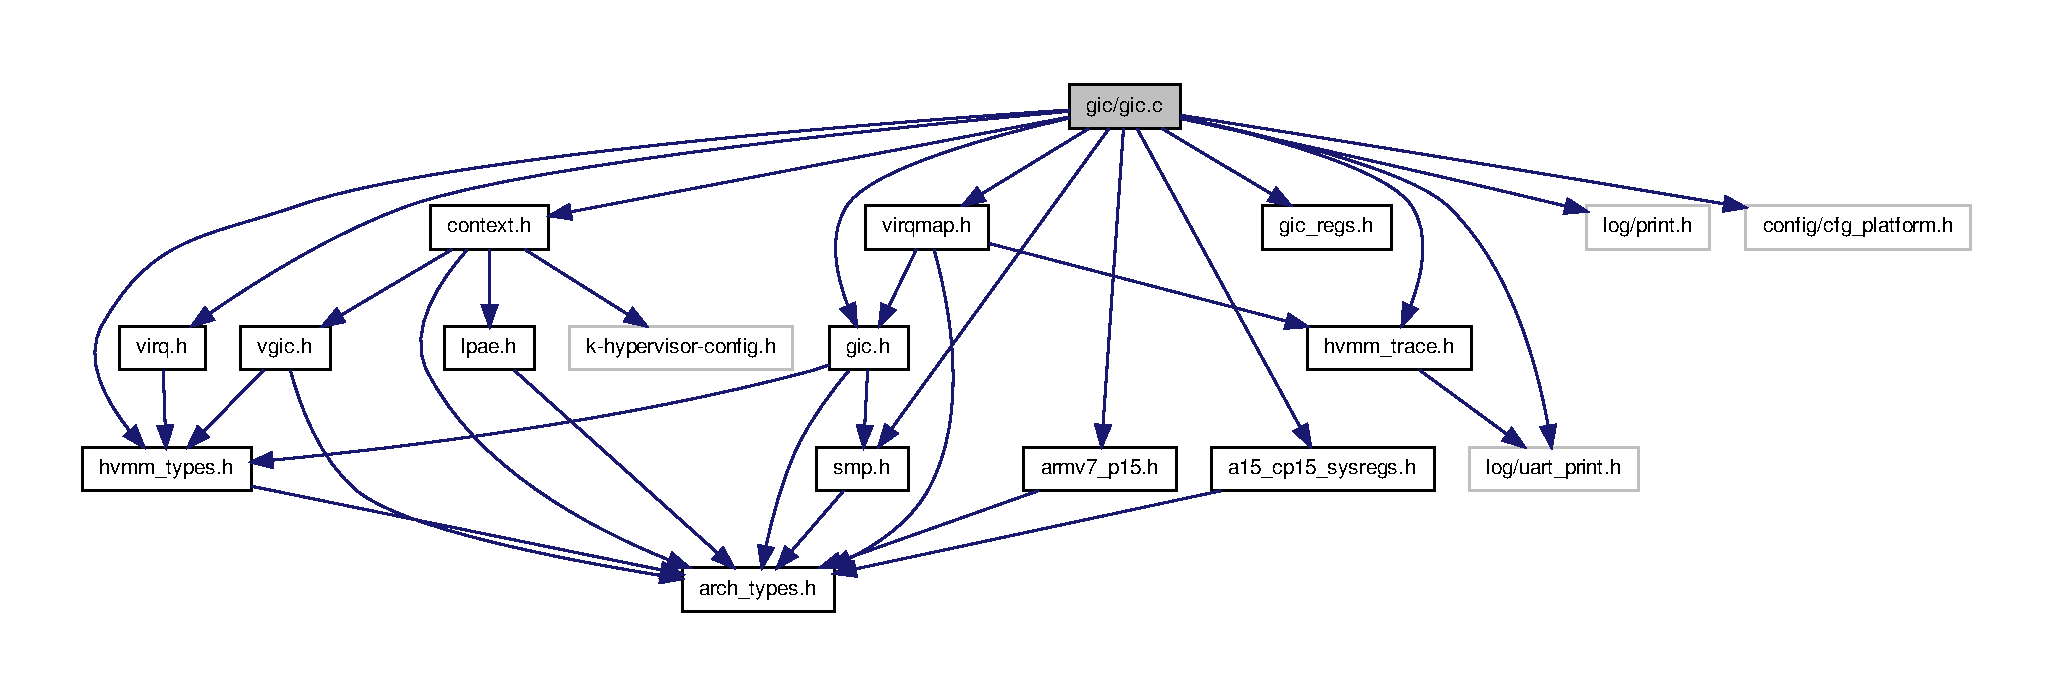
\includegraphics[width=350pt]{gic_8c__incl}
\end{center}
\end{figure}
\subsection*{\-Data \-Structures}
\begin{DoxyCompactItemize}
\item 
struct \hyperlink{structgic}{gic}
\end{DoxyCompactItemize}
\subsection*{\-Defines}
\begin{DoxyCompactItemize}
\item 
\#define \hyperlink{gic_8c_a636ebe1049205391c94c87fb73751cd3}{\-C\-B\-A\-R\-\_\-\-P\-E\-R\-I\-P\-H\-B\-A\-S\-E\-\_\-\-M\-S\-B\-\_\-\-M\-A\-S\-K}~0x000000\-F\-F
\item 
\#define \hyperlink{gic_8c_a30ca90ad0e327260a65618197261f4f2}{\-A\-R\-M\-\_\-\-C\-P\-U\-I\-D\-\_\-\-C\-O\-R\-T\-E\-X\-A15}~0x412fc0f1
\item 
\#define \hyperlink{gic_8c_aafc97bc5f4bc00a3153f9f7a42a75084}{\-M\-I\-D\-R\-\_\-\-M\-A\-S\-K\-\_\-\-P\-P\-N}~(0x0\-F\-F\-F $<$$<$4)
\item 
\#define \hyperlink{gic_8c_a98c20b3bc1389721882e5614f64f4c86}{\-M\-I\-D\-R\-\_\-\-P\-P\-N\-\_\-\-C\-O\-R\-T\-E\-X\-A15}~(0x\-C0\-F $<$$<$ 4)
\item 
\#define \hyperlink{gic_8c_ae03ba1b0ce9d92968e25bfc5137b6141}{\-G\-I\-C\-\_\-\-I\-N\-T\-\_\-\-P\-R\-I\-O\-R\-I\-T\-Y\-\_\-\-D\-E\-F\-A\-U\-L\-T\-\_\-\-W\-O\-R\-D}
\item 
\#define \hyperlink{gic_8c_abf8cb594c336c07b1ed464f49ffd7848}{\-G\-I\-C\-\_\-\-S\-I\-G\-N\-A\-T\-U\-R\-E\-\_\-\-I\-N\-I\-T\-I\-A\-L\-I\-Z\-E\-D}~0x5108\-E\-A\-D7
\end{DoxyCompactItemize}
\subsection*{\-Functions}
\begin{DoxyCompactItemize}
\item 
static void \hyperlink{gic_8c_a355755273aee03b63c4a9aa6e7e4a95e}{gic\-\_\-dump\-\_\-registers} (void)
\item 
static \hyperlink{arch__types_8h_aaa5d1cd013383c889537491c3cfd9aad}{uint64\-\_\-t} \hyperlink{gic_8c_a571d07e36235ca9d298c086e117e2bb1}{gic\-\_\-periphbase\-\_\-pa} (void)
\item 
static \hyperlink{hvmm__types_8h_a39d593b2c97852f566d7472b76ab7ba2}{hvmm\-\_\-status\-\_\-t} \hyperlink{gic_8c_ac9cad87ffdf3a3e1cde6002ea3f347a9}{gic\-\_\-init\-\_\-baseaddr} (\hyperlink{arch__types_8h_a435d1572bf3f880d55459d9805097f62}{uint32\-\_\-t} $\ast$va\-\_\-base)
\item 
static \hyperlink{hvmm__types_8h_a39d593b2c97852f566d7472b76ab7ba2}{hvmm\-\_\-status\-\_\-t} \hyperlink{gic_8c_a592c46444cc3e5696daa78bedbbe31f3}{gic\-\_\-init\-\_\-dist} (void)
\item 
static \hyperlink{hvmm__types_8h_a39d593b2c97852f566d7472b76ab7ba2}{hvmm\-\_\-status\-\_\-t} \hyperlink{gic_8c_a8395d48667bdc01bce88521812a39f53}{gic\-\_\-init\-\_\-cpui} (void)
\item 
\hyperlink{hvmm__types_8h_a39d593b2c97852f566d7472b76ab7ba2}{hvmm\-\_\-status\-\_\-t} \hyperlink{gic_8c_a53e36754e628b6624a760838e37fd9df}{gic\-\_\-enable\-\_\-irq} (\hyperlink{arch__types_8h_a435d1572bf3f880d55459d9805097f62}{uint32\-\_\-t} irq)
\item 
\hyperlink{hvmm__types_8h_a39d593b2c97852f566d7472b76ab7ba2}{hvmm\-\_\-status\-\_\-t} \hyperlink{gic_8c_ac9a2d7f5ce83d3499113a8566f65fad0}{gic\-\_\-disable\-\_\-irq} (\hyperlink{arch__types_8h_a435d1572bf3f880d55459d9805097f62}{uint32\-\_\-t} irq)
\item 
\hyperlink{hvmm__types_8h_a39d593b2c97852f566d7472b76ab7ba2}{hvmm\-\_\-status\-\_\-t} \hyperlink{gic_8c_a7a8d9c8017d6bcc6fc377b52ed6b74c1}{gic\-\_\-deactivate\-\_\-irq} (\hyperlink{arch__types_8h_a435d1572bf3f880d55459d9805097f62}{uint32\-\_\-t} irq)
\item 
\hyperlink{hvmm__types_8h_a39d593b2c97852f566d7472b76ab7ba2}{hvmm\-\_\-status\-\_\-t} \hyperlink{gic_8c_aaee4d58fadbe09c39f45e8e114a4dd4d}{gic\-\_\-test\-\_\-set\-\_\-irq\-\_\-handler} (int irq, \hyperlink{gic_8h_a4b1f3150431142b6910f651a1172f446}{gic\-\_\-irq\-\_\-handler\-\_\-t} handler, void $\ast$pdata)
\item 
volatile \hyperlink{arch__types_8h_a435d1572bf3f880d55459d9805097f62}{uint32\-\_\-t} $\ast$ \hyperlink{gic_8c_a608941cbc8ab5a657834d451f0368a6e}{gic\-\_\-vgic\-\_\-baseaddr} (void)
\item 
\hyperlink{hvmm__types_8h_a39d593b2c97852f566d7472b76ab7ba2}{hvmm\-\_\-status\-\_\-t} \hyperlink{gic_8c_a0913d7e2dc598b3eb2cb09c4a1185cbe}{gic\-\_\-init} (void)
\item 
\hyperlink{hvmm__types_8h_a39d593b2c97852f566d7472b76ab7ba2}{hvmm\-\_\-status\-\_\-t} \hyperlink{gic_8c_acbe5581611f81cd00b58cebeda222edf}{gic\-\_\-test\-\_\-configure\-\_\-irq} (\hyperlink{arch__types_8h_a435d1572bf3f880d55459d9805097f62}{uint32\-\_\-t} irq, \hyperlink{gic_8h_a1f4bb652388c46210cea87dfa0d0da83}{gic\-\_\-int\-\_\-polarity\-\_\-t} polarity, \hyperlink{arch__types_8h_aba7bc1797add20fe3efdf37ced1182c5}{uint8\-\_\-t} cpumask, \hyperlink{arch__types_8h_aba7bc1797add20fe3efdf37ced1182c5}{uint8\-\_\-t} priority)
\item 
void \hyperlink{gic_8c_a55735be7cf847ae8064b56d22bd80831}{gic\-\_\-interrupt} (int fiq, void $\ast$pregs)
\end{DoxyCompactItemize}
\subsection*{\-Variables}
\begin{DoxyCompactItemize}
\item 
static struct \hyperlink{structgic}{gic} \hyperlink{gic_8c_a812e13a3081e93998d02dcad7c12f64b}{\-\_\-gic}
\end{DoxyCompactItemize}


\subsection{\-Define \-Documentation}
\hypertarget{gic_8c_a30ca90ad0e327260a65618197261f4f2}{\index{gic.\-c@{gic.\-c}!\-A\-R\-M\-\_\-\-C\-P\-U\-I\-D\-\_\-\-C\-O\-R\-T\-E\-X\-A15@{\-A\-R\-M\-\_\-\-C\-P\-U\-I\-D\-\_\-\-C\-O\-R\-T\-E\-X\-A15}}
\index{\-A\-R\-M\-\_\-\-C\-P\-U\-I\-D\-\_\-\-C\-O\-R\-T\-E\-X\-A15@{\-A\-R\-M\-\_\-\-C\-P\-U\-I\-D\-\_\-\-C\-O\-R\-T\-E\-X\-A15}!gic.c@{gic.\-c}}
\subsubsection[{\-A\-R\-M\-\_\-\-C\-P\-U\-I\-D\-\_\-\-C\-O\-R\-T\-E\-X\-A15}]{\setlength{\rightskip}{0pt plus 5cm}\#define {\bf \-A\-R\-M\-\_\-\-C\-P\-U\-I\-D\-\_\-\-C\-O\-R\-T\-E\-X\-A15}~0x412fc0f1}}\label{gic_8c_a30ca90ad0e327260a65618197261f4f2}


\-Definition at line 18 of file gic.\-c.

\hypertarget{gic_8c_a636ebe1049205391c94c87fb73751cd3}{\index{gic.\-c@{gic.\-c}!\-C\-B\-A\-R\-\_\-\-P\-E\-R\-I\-P\-H\-B\-A\-S\-E\-\_\-\-M\-S\-B\-\_\-\-M\-A\-S\-K@{\-C\-B\-A\-R\-\_\-\-P\-E\-R\-I\-P\-H\-B\-A\-S\-E\-\_\-\-M\-S\-B\-\_\-\-M\-A\-S\-K}}
\index{\-C\-B\-A\-R\-\_\-\-P\-E\-R\-I\-P\-H\-B\-A\-S\-E\-\_\-\-M\-S\-B\-\_\-\-M\-A\-S\-K@{\-C\-B\-A\-R\-\_\-\-P\-E\-R\-I\-P\-H\-B\-A\-S\-E\-\_\-\-M\-S\-B\-\_\-\-M\-A\-S\-K}!gic.c@{gic.\-c}}
\subsubsection[{\-C\-B\-A\-R\-\_\-\-P\-E\-R\-I\-P\-H\-B\-A\-S\-E\-\_\-\-M\-S\-B\-\_\-\-M\-A\-S\-K}]{\setlength{\rightskip}{0pt plus 5cm}\#define {\bf \-C\-B\-A\-R\-\_\-\-P\-E\-R\-I\-P\-H\-B\-A\-S\-E\-\_\-\-M\-S\-B\-\_\-\-M\-A\-S\-K}~0x000000\-F\-F}}\label{gic_8c_a636ebe1049205391c94c87fb73751cd3}


\-Definition at line 16 of file gic.\-c.

\hypertarget{gic_8c_ae03ba1b0ce9d92968e25bfc5137b6141}{\index{gic.\-c@{gic.\-c}!\-G\-I\-C\-\_\-\-I\-N\-T\-\_\-\-P\-R\-I\-O\-R\-I\-T\-Y\-\_\-\-D\-E\-F\-A\-U\-L\-T\-\_\-\-W\-O\-R\-D@{\-G\-I\-C\-\_\-\-I\-N\-T\-\_\-\-P\-R\-I\-O\-R\-I\-T\-Y\-\_\-\-D\-E\-F\-A\-U\-L\-T\-\_\-\-W\-O\-R\-D}}
\index{\-G\-I\-C\-\_\-\-I\-N\-T\-\_\-\-P\-R\-I\-O\-R\-I\-T\-Y\-\_\-\-D\-E\-F\-A\-U\-L\-T\-\_\-\-W\-O\-R\-D@{\-G\-I\-C\-\_\-\-I\-N\-T\-\_\-\-P\-R\-I\-O\-R\-I\-T\-Y\-\_\-\-D\-E\-F\-A\-U\-L\-T\-\_\-\-W\-O\-R\-D}!gic.c@{gic.\-c}}
\subsubsection[{\-G\-I\-C\-\_\-\-I\-N\-T\-\_\-\-P\-R\-I\-O\-R\-I\-T\-Y\-\_\-\-D\-E\-F\-A\-U\-L\-T\-\_\-\-W\-O\-R\-D}]{\setlength{\rightskip}{0pt plus 5cm}\#define {\bf \-G\-I\-C\-\_\-\-I\-N\-T\-\_\-\-P\-R\-I\-O\-R\-I\-T\-Y\-\_\-\-D\-E\-F\-A\-U\-L\-T\-\_\-\-W\-O\-R\-D}}}\label{gic_8c_ae03ba1b0ce9d92968e25bfc5137b6141}
{\bfseries \-Value\-:}
\begin{DoxyCode}
( (GIC_INT_PRIORITY_DEFAULT << 24 ) \
                                         |(GIC_INT_PRIORITY_DEFAULT << 16 ) \
                                         |(GIC_INT_PRIORITY_DEFAULT << 8 ) \
                                         |(GIC_INT_PRIORITY_DEFAULT ) )
\end{DoxyCode}


\-Definition at line 24 of file gic.\-c.

\hypertarget{gic_8c_abf8cb594c336c07b1ed464f49ffd7848}{\index{gic.\-c@{gic.\-c}!\-G\-I\-C\-\_\-\-S\-I\-G\-N\-A\-T\-U\-R\-E\-\_\-\-I\-N\-I\-T\-I\-A\-L\-I\-Z\-E\-D@{\-G\-I\-C\-\_\-\-S\-I\-G\-N\-A\-T\-U\-R\-E\-\_\-\-I\-N\-I\-T\-I\-A\-L\-I\-Z\-E\-D}}
\index{\-G\-I\-C\-\_\-\-S\-I\-G\-N\-A\-T\-U\-R\-E\-\_\-\-I\-N\-I\-T\-I\-A\-L\-I\-Z\-E\-D@{\-G\-I\-C\-\_\-\-S\-I\-G\-N\-A\-T\-U\-R\-E\-\_\-\-I\-N\-I\-T\-I\-A\-L\-I\-Z\-E\-D}!gic.c@{gic.\-c}}
\subsubsection[{\-G\-I\-C\-\_\-\-S\-I\-G\-N\-A\-T\-U\-R\-E\-\_\-\-I\-N\-I\-T\-I\-A\-L\-I\-Z\-E\-D}]{\setlength{\rightskip}{0pt plus 5cm}\#define {\bf \-G\-I\-C\-\_\-\-S\-I\-G\-N\-A\-T\-U\-R\-E\-\_\-\-I\-N\-I\-T\-I\-A\-L\-I\-Z\-E\-D}~0x5108\-E\-A\-D7}}\label{gic_8c_abf8cb594c336c07b1ed464f49ffd7848}


\-Definition at line 29 of file gic.\-c.

\hypertarget{gic_8c_aafc97bc5f4bc00a3153f9f7a42a75084}{\index{gic.\-c@{gic.\-c}!\-M\-I\-D\-R\-\_\-\-M\-A\-S\-K\-\_\-\-P\-P\-N@{\-M\-I\-D\-R\-\_\-\-M\-A\-S\-K\-\_\-\-P\-P\-N}}
\index{\-M\-I\-D\-R\-\_\-\-M\-A\-S\-K\-\_\-\-P\-P\-N@{\-M\-I\-D\-R\-\_\-\-M\-A\-S\-K\-\_\-\-P\-P\-N}!gic.c@{gic.\-c}}
\subsubsection[{\-M\-I\-D\-R\-\_\-\-M\-A\-S\-K\-\_\-\-P\-P\-N}]{\setlength{\rightskip}{0pt plus 5cm}\#define {\bf \-M\-I\-D\-R\-\_\-\-M\-A\-S\-K\-\_\-\-P\-P\-N}~(0x0\-F\-F\-F $<$$<$4)}}\label{gic_8c_aafc97bc5f4bc00a3153f9f7a42a75084}


\-Definition at line 20 of file gic.\-c.

\hypertarget{gic_8c_a98c20b3bc1389721882e5614f64f4c86}{\index{gic.\-c@{gic.\-c}!\-M\-I\-D\-R\-\_\-\-P\-P\-N\-\_\-\-C\-O\-R\-T\-E\-X\-A15@{\-M\-I\-D\-R\-\_\-\-P\-P\-N\-\_\-\-C\-O\-R\-T\-E\-X\-A15}}
\index{\-M\-I\-D\-R\-\_\-\-P\-P\-N\-\_\-\-C\-O\-R\-T\-E\-X\-A15@{\-M\-I\-D\-R\-\_\-\-P\-P\-N\-\_\-\-C\-O\-R\-T\-E\-X\-A15}!gic.c@{gic.\-c}}
\subsubsection[{\-M\-I\-D\-R\-\_\-\-P\-P\-N\-\_\-\-C\-O\-R\-T\-E\-X\-A15}]{\setlength{\rightskip}{0pt plus 5cm}\#define {\bf \-M\-I\-D\-R\-\_\-\-P\-P\-N\-\_\-\-C\-O\-R\-T\-E\-X\-A15}~(0x\-C0\-F $<$$<$ 4)}}\label{gic_8c_a98c20b3bc1389721882e5614f64f4c86}


\-Definition at line 21 of file gic.\-c.



\subsection{\-Function \-Documentation}
\hypertarget{gic_8c_a7a8d9c8017d6bcc6fc377b52ed6b74c1}{\index{gic.\-c@{gic.\-c}!gic\-\_\-deactivate\-\_\-irq@{gic\-\_\-deactivate\-\_\-irq}}
\index{gic\-\_\-deactivate\-\_\-irq@{gic\-\_\-deactivate\-\_\-irq}!gic.c@{gic.\-c}}
\subsubsection[{gic\-\_\-deactivate\-\_\-irq}]{\setlength{\rightskip}{0pt plus 5cm}{\bf hvmm\-\_\-status\-\_\-t} {\bf gic\-\_\-deactivate\-\_\-irq} (
\begin{DoxyParamCaption}
\item[{{\bf uint32\-\_\-t}}]{irq}
\end{DoxyParamCaption}
)}}\label{gic_8c_a7a8d9c8017d6bcc6fc377b52ed6b74c1}


\-Definition at line 220 of file gic.\-c.


\begin{DoxyCode}
{
    _gic.ba_gicc[GICC_DIR] = irq;
    return HVMM_STATUS_SUCCESS;
}
\end{DoxyCode}
\hypertarget{gic_8c_ac9a2d7f5ce83d3499113a8566f65fad0}{\index{gic.\-c@{gic.\-c}!gic\-\_\-disable\-\_\-irq@{gic\-\_\-disable\-\_\-irq}}
\index{gic\-\_\-disable\-\_\-irq@{gic\-\_\-disable\-\_\-irq}!gic.c@{gic.\-c}}
\subsubsection[{gic\-\_\-disable\-\_\-irq}]{\setlength{\rightskip}{0pt plus 5cm}{\bf hvmm\-\_\-status\-\_\-t} {\bf gic\-\_\-disable\-\_\-irq} (
\begin{DoxyParamCaption}
\item[{{\bf uint32\-\_\-t}}]{irq}
\end{DoxyParamCaption}
)}}\label{gic_8c_ac9a2d7f5ce83d3499113a8566f65fad0}


\-Definition at line 214 of file gic.\-c.


\begin{DoxyCode}
{
    _gic.ba_gicd[GICD_ICENABLER + irq / 32] = (1u << (irq % 32));
    return HVMM_STATUS_SUCCESS;
}
\end{DoxyCode}
\hypertarget{gic_8c_a355755273aee03b63c4a9aa6e7e4a95e}{\index{gic.\-c@{gic.\-c}!gic\-\_\-dump\-\_\-registers@{gic\-\_\-dump\-\_\-registers}}
\index{gic\-\_\-dump\-\_\-registers@{gic\-\_\-dump\-\_\-registers}!gic.c@{gic.\-c}}
\subsubsection[{gic\-\_\-dump\-\_\-registers}]{\setlength{\rightskip}{0pt plus 5cm}static void {\bf gic\-\_\-dump\-\_\-registers} (
\begin{DoxyParamCaption}
\item[{void}]{}
\end{DoxyParamCaption}
)\hspace{0.3cm}{\ttfamily  \mbox{[}static\mbox{]}}}}\label{gic_8c_a355755273aee03b63c4a9aa6e7e4a95e}


\-Definition at line 46 of file gic.\-c.


\begin{DoxyCode}
{

    uint32_t midr;

    HVMM_TRACE_ENTER();

    midr = read_midr();
    uart_print( "midr:"); uart_print_hex32(midr); uart_print("\n\r");

    if ( (midr & MIDR_MASK_PPN) == MIDR_PPN_CORTEXA15) {
        uint32_t value;
        uart_print( "cbar:"); uart_print_hex32(_gic.baseaddr); uart_print("\n\r
      ");
        uart_print( "ba_gicd:"); uart_print_hex32((uint32_t)_gic.ba_gicd); 
      uart_print("\n\r");
        uart_print( "ba_gicc:"); uart_print_hex32((uint32_t)_gic.ba_gicc); 
      uart_print("\n\r");
        uart_print( "ba_gich:"); uart_print_hex32((uint32_t)_gic.ba_gich); 
      uart_print("\n\r");
        uart_print( "ba_gicv:"); uart_print_hex32((uint32_t)_gic.ba_gicv); 
      uart_print("\n\r");
        uart_print( "ba_gicvi:"); uart_print_hex32((uint32_t)_gic.ba_gicvi); 
      uart_print("\n\r");
        value = _gic.ba_gicd[GICD_CTLR]; uart_print( "GICD_CTLR:"); 
      uart_print_hex32(value); uart_print("\n\r");
        value = _gic.ba_gicd[GICD_TYPER]; uart_print( "GICD_TYPER:"); 
      uart_print_hex32(value); uart_print("\n\r");
        value = _gic.ba_gicd[GICD_IIDR]; uart_print( "GICD_IIDR:"); 
      uart_print_hex32(value); uart_print("\n\r");
    }
    HVMM_TRACE_EXIT();
}
\end{DoxyCode}
\hypertarget{gic_8c_a53e36754e628b6624a760838e37fd9df}{\index{gic.\-c@{gic.\-c}!gic\-\_\-enable\-\_\-irq@{gic\-\_\-enable\-\_\-irq}}
\index{gic\-\_\-enable\-\_\-irq@{gic\-\_\-enable\-\_\-irq}!gic.c@{gic.\-c}}
\subsubsection[{gic\-\_\-enable\-\_\-irq}]{\setlength{\rightskip}{0pt plus 5cm}{\bf hvmm\-\_\-status\-\_\-t} {\bf gic\-\_\-enable\-\_\-irq} (
\begin{DoxyParamCaption}
\item[{{\bf uint32\-\_\-t}}]{irq}
\end{DoxyParamCaption}
)}}\label{gic_8c_a53e36754e628b6624a760838e37fd9df}


\-Definition at line 208 of file gic.\-c.


\begin{DoxyCode}
{
    _gic.ba_gicd[GICD_ISENABLER + irq / 32] = (1u << (irq % 32));
    return HVMM_STATUS_SUCCESS;
}
\end{DoxyCode}
\hypertarget{gic_8c_a0913d7e2dc598b3eb2cb09c4a1185cbe}{\index{gic.\-c@{gic.\-c}!gic\-\_\-init@{gic\-\_\-init}}
\index{gic\-\_\-init@{gic\-\_\-init}!gic.c@{gic.\-c}}
\subsubsection[{gic\-\_\-init}]{\setlength{\rightskip}{0pt plus 5cm}{\bf hvmm\-\_\-status\-\_\-t} {\bf gic\-\_\-init} (
\begin{DoxyParamCaption}
\item[{void}]{}
\end{DoxyParamCaption}
)}}\label{gic_8c_a0913d7e2dc598b3eb2cb09c4a1185cbe}


\-Definition at line 247 of file gic.\-c.


\begin{DoxyCode}
{
    hvmm_status_t result = HVMM_STATUS_UNKNOWN_ERROR;
    int i;

    HVMM_TRACE_ENTER();

    for( i = 0; i < GIC_NUM_MAX_IRQS; i++) {
        _gic.handlers[i] = 0;
    }
    
    /*
     * Determining VA of GIC base adddress has not been defined yet. Let is use
       the PA for the time being
     */
    result = gic_init_baseaddr((void*)CFG_GIC_BASE_PA);

    if ( result == HVMM_STATUS_SUCCESS ) {
        gic_dump_registers();
    }

    /*
     * Initialize and Enable GIC Distributor
     */
    if ( result == HVMM_STATUS_SUCCESS ) {
        result = gic_init_dist();
    }

    /*
     * Initialize and Enable GIC CPU Interface for this CPU
     */
    if ( result == HVMM_STATUS_SUCCESS ) {
        result = gic_init_cpui();
    }
    if ( result == HVMM_STATUS_SUCCESS ) {
        _gic.initialized = GIC_SIGNATURE_INITIALIZED;
    }

    HVMM_TRACE_EXIT();
    return result;
}
\end{DoxyCode}


\-Here is the call graph for this function\-:
\nopagebreak
\begin{figure}[H]
\begin{center}
\leavevmode
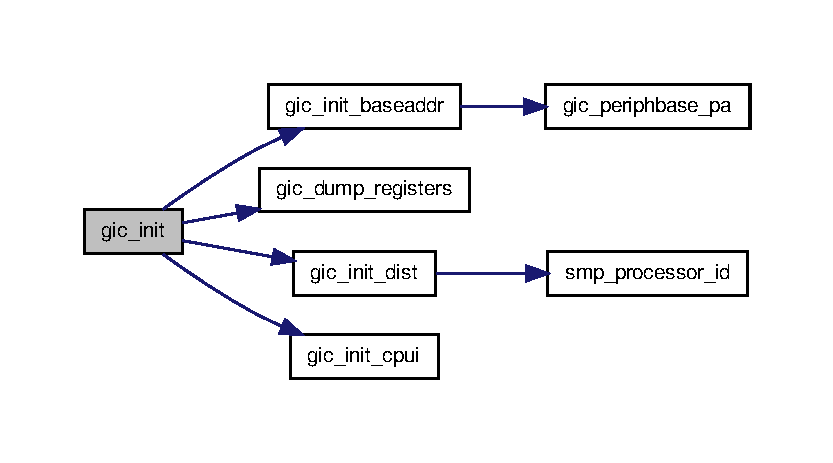
\includegraphics[width=350pt]{gic_8c_a0913d7e2dc598b3eb2cb09c4a1185cbe_cgraph}
\end{center}
\end{figure}


\hypertarget{gic_8c_ac9cad87ffdf3a3e1cde6002ea3f347a9}{\index{gic.\-c@{gic.\-c}!gic\-\_\-init\-\_\-baseaddr@{gic\-\_\-init\-\_\-baseaddr}}
\index{gic\-\_\-init\-\_\-baseaddr@{gic\-\_\-init\-\_\-baseaddr}!gic.c@{gic.\-c}}
\subsubsection[{gic\-\_\-init\-\_\-baseaddr}]{\setlength{\rightskip}{0pt plus 5cm}static {\bf hvmm\-\_\-status\-\_\-t} {\bf gic\-\_\-init\-\_\-baseaddr} (
\begin{DoxyParamCaption}
\item[{{\bf uint32\-\_\-t} $\ast$}]{va\-\_\-base}
\end{DoxyParamCaption}
)\hspace{0.3cm}{\ttfamily  \mbox{[}static\mbox{]}}}}\label{gic_8c_ac9cad87ffdf3a3e1cde6002ea3f347a9}


\-Definition at line 86 of file gic.\-c.


\begin{DoxyCode}
{
// MIDR[15:4], CRn:c0, Op1:0, CRm:c0, Op2:0  == 0xC0F (Cortex-A15)
// Cortex-A15 C15 System Control, C15 Registers
// Name: Op1, CRm, Op2
    uint32_t midr;
    hvmm_status_t result = HVMM_STATUS_UNKNOWN_ERROR;

    HVMM_TRACE_ENTER();

    midr = read_midr();
    uart_print( "midr:"); uart_print_hex32(midr); uart_print("\n\r");

    /* 
     * Note:
     * We currently support GICv2 with Cortex-A15 only. 
     * Other architectures with GICv2 support will be further listed and added
       for support later
     */
    if ( (midr & MIDR_MASK_PPN) == MIDR_PPN_CORTEXA15) {
        /* fall-back to periphbase addr from cbar */
        if ( va_base == 0 ) va_base = (uint32_t *) (uint32_t) (gic_periphbase_pa
      () & 0x00000000FFFFFFFFULL);
        _gic.baseaddr = (uint32_t) va_base;
        uart_print( "cbar:"); uart_print_hex32(_gic.baseaddr); uart_print("\n\r
      ");
        _gic.ba_gicd = (uint32_t *) (_gic.baseaddr + GIC_OFFSET_GICD);
        _gic.ba_gicc = (uint32_t *) (_gic.baseaddr + GIC_OFFSET_GICC);
        _gic.ba_gich = (uint32_t *) (_gic.baseaddr + GIC_OFFSET_GICH);
        _gic.ba_gicv = (uint32_t *) (_gic.baseaddr + GIC_OFFSET_GICV);
        _gic.ba_gicvi = (uint32_t *) (_gic.baseaddr + GIC_OFFSET_GICVI);

        result = HVMM_STATUS_SUCCESS;
    } else {
        uart_print( "GICv2 Unsupported\n\r" );
        uart_print( "midr.ppn:"); uart_print_hex32(midr & MIDR_MASK_PPN); 
      uart_print("\n\r");

        result = HVMM_STATUS_UNSUPPORTED_FEATURE;
    }

    HVMM_TRACE_EXIT();
    return result;
}
\end{DoxyCode}


\-Here is the call graph for this function\-:
\nopagebreak
\begin{figure}[H]
\begin{center}
\leavevmode
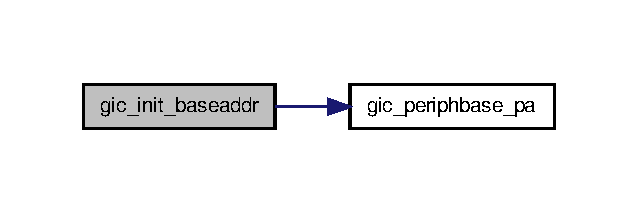
\includegraphics[width=306pt]{gic_8c_ac9cad87ffdf3a3e1cde6002ea3f347a9_cgraph}
\end{center}
\end{figure}


\hypertarget{gic_8c_a8395d48667bdc01bce88521812a39f53}{\index{gic.\-c@{gic.\-c}!gic\-\_\-init\-\_\-cpui@{gic\-\_\-init\-\_\-cpui}}
\index{gic\-\_\-init\-\_\-cpui@{gic\-\_\-init\-\_\-cpui}!gic.c@{gic.\-c}}
\subsubsection[{gic\-\_\-init\-\_\-cpui}]{\setlength{\rightskip}{0pt plus 5cm}static {\bf hvmm\-\_\-status\-\_\-t} {\bf gic\-\_\-init\-\_\-cpui} (
\begin{DoxyParamCaption}
\item[{void}]{}
\end{DoxyParamCaption}
)\hspace{0.3cm}{\ttfamily  \mbox{[}static\mbox{]}}}}\label{gic_8c_a8395d48667bdc01bce88521812a39f53}


\-Definition at line 181 of file gic.\-c.


\begin{DoxyCode}
{
    hvmm_status_t result = HVMM_STATUS_UNKNOWN_ERROR;
    int i;

    /* Disable forwarding PPIs(ID16~31) */
    _gic.ba_gicd[GICD_ICENABLER] = 0xFFFF0000;
    /* Enable forwarding SGIs(ID0~15) */
    _gic.ba_gicd[GICD_ISENABLER] = 0x0000FFFF;
    
    /* Default priority for SGIs and PPIs */
    for( i = 0; i < 32; i += 4 ) {
        _gic.ba_gicd[GICD_IPRIORITYR | i/4] = GIC_INT_PRIORITY_DEFAULT_WORD;
    }

    /* No Priority Masking: the lowest value as the threshold : 255 */
    _gic.ba_gicc[GICC_PMR] = 0xFF;
    _gic.ba_gicc[GICC_BPR] = 0x0;

    /* Enable signaling of interrupts and GICC_EOIR only drops priority */
    _gic.ba_gicc[GICC_CTLR] = GICC_CTL_ENABLE | GICC_CTL_EOI;

    result = HVMM_STATUS_SUCCESS;
    return result;
}
\end{DoxyCode}
\hypertarget{gic_8c_a592c46444cc3e5696daa78bedbbe31f3}{\index{gic.\-c@{gic.\-c}!gic\-\_\-init\-\_\-dist@{gic\-\_\-init\-\_\-dist}}
\index{gic\-\_\-init\-\_\-dist@{gic\-\_\-init\-\_\-dist}!gic.c@{gic.\-c}}
\subsubsection[{gic\-\_\-init\-\_\-dist}]{\setlength{\rightskip}{0pt plus 5cm}static {\bf hvmm\-\_\-status\-\_\-t} {\bf gic\-\_\-init\-\_\-dist} (
\begin{DoxyParamCaption}
\item[{void}]{}
\end{DoxyParamCaption}
)\hspace{0.3cm}{\ttfamily  \mbox{[}static\mbox{]}}}}\label{gic_8c_a592c46444cc3e5696daa78bedbbe31f3}


\-Definition at line 128 of file gic.\-c.


\begin{DoxyCode}
{
    uint32_t type;
    int i;
    uint32_t cpumask;

    HVMM_TRACE_ENTER();

    /* Disable Distributor */
    _gic.ba_gicd[GICD_CTLR] = 0;

    type = _gic.ba_gicd[GICD_TYPER];
    _gic.lines = 32 * ((type & GICD_TYPE_LINES_MASK) + 1);
    _gic.cpus = 1 + ((type & GICD_TYPE_CPUS_MASK) >> GICD_TYPE_CPUS_SHIFT);
    uart_print( "GIC: lines:"); uart_print_hex32(_gic.lines ); 
    uart_print( " cpus:"); uart_print_hex32(_gic.cpus);
    uart_print( " IID:" ); uart_print_hex32(_gic.ba_gicd[GICD_IIDR]); 
      uart_print("\n\r");

    /* Interrupt polarity for SPIs (Global Interrupts) active-low */
    for( i = 32; i < _gic.lines; i += 16 ) {
        _gic.ba_gicd[GICD_ICFGR + i / 16] = 0x0;
    }

    /* Default Priority for all Interrupts
     * Private/Banked interrupts will be configured separately 
     */
    for( i = 32; i < _gic.lines; i+= 4 ) {
        _gic.ba_gicd[GICD_IPRIORITYR + i / 4] = GIC_INT_PRIORITY_DEFAULT_WORD;
    }

    /* Disable all global interrupts. 
     * Private/Banked interrupts will be configured separately 
     */
    for( i = 32; i < _gic.lines; i+= 32 ) {
        _gic.ba_gicd[GICD_ICENABLER + i / 32] = 0xFFFFFFFF;
    }

    /* Route all global IRQs to this CPU */
    cpumask = 1 << smp_processor_id();
    cpumask |= cpumask << 8;
    cpumask |= cpumask << 16;
    for( i = 32; i < _gic.lines; i += 4 ) {
        _gic.ba_gicd[GICD_ITARGETSR + i / 4] = cpumask;
    }


    /* Enable Distributor */
    _gic.ba_gicd[GICD_CTLR] = GICD_CTLR_ENABLE;
    HVMM_TRACE_EXIT();
    return HVMM_STATUS_SUCCESS;
}
\end{DoxyCode}


\-Here is the call graph for this function\-:
\nopagebreak
\begin{figure}[H]
\begin{center}
\leavevmode
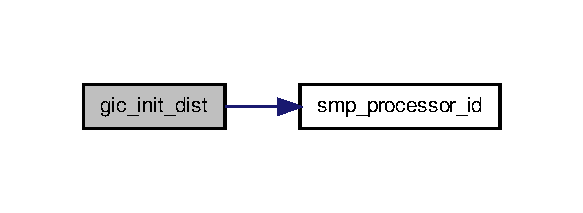
\includegraphics[width=280pt]{gic_8c_a592c46444cc3e5696daa78bedbbe31f3_cgraph}
\end{center}
\end{figure}


\hypertarget{gic_8c_a55735be7cf847ae8064b56d22bd80831}{\index{gic.\-c@{gic.\-c}!gic\-\_\-interrupt@{gic\-\_\-interrupt}}
\index{gic\-\_\-interrupt@{gic\-\_\-interrupt}!gic.c@{gic.\-c}}
\subsubsection[{gic\-\_\-interrupt}]{\setlength{\rightskip}{0pt plus 5cm}void {\bf gic\-\_\-interrupt} (
\begin{DoxyParamCaption}
\item[{int}]{fiq, }
\item[{void $\ast$}]{pregs}
\end{DoxyParamCaption}
)}}\label{gic_8c_a55735be7cf847ae8064b56d22bd80831}


\-Definition at line 337 of file gic.\-c.


\begin{DoxyCode}
{
    /*
     * 1. ACK - CPU Interface - GICC_IAR read
     * 2. Completion - CPU Interface - GICC_EOIR
     * 2.1 Deactivation - CPU Interface - GICC_DIR
     */
    uint32_t iar;

    uint32_t irq;
    struct arch_regs *regs = pregs;
    const struct virqmap_entry *virq_entry;

    /* ACK */
    iar = _gic.ba_gicc[GICC_IAR];
    irq = iar & GICC_IAR_INTID_MASK;
    if ( irq < _gic.lines ) {
        virq_entry = virqmap_for_pirq(irq);

        /* ISR */
        printh( "ISR(irq):%x\n", irq);

        /* IRQ INJECTION */
        if(virq_entry != VIRQMAP_ENTRY_NOTFOUND) { 

            /* priority drop only for hanlding irq in guest */
            _gic.ba_gicc[GICC_EOIR] = irq;
            virq_inject(virq_entry->vmid, virq_entry->virq, irq, 1);

        } else {

            if ( _gic.handlers[irq] ) {
                _gic.handlers[irq]( irq, regs, 0 );
            }

            /* Completion & Deactivation */
            _gic.ba_gicc[GICC_EOIR] = irq;
            _gic.ba_gicc[GICC_DIR] = irq;
        }
    } else {
        printh( "gic:no pending irq:%x\n", irq);
    }
}
\end{DoxyCode}


\-Here is the call graph for this function\-:
\nopagebreak
\begin{figure}[H]
\begin{center}
\leavevmode
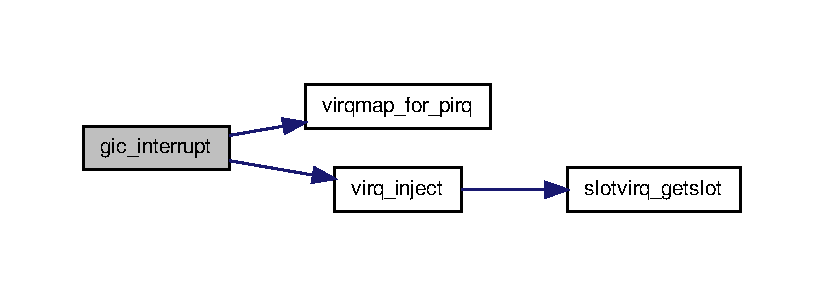
\includegraphics[width=350pt]{gic_8c_a55735be7cf847ae8064b56d22bd80831_cgraph}
\end{center}
\end{figure}


\hypertarget{gic_8c_a571d07e36235ca9d298c086e117e2bb1}{\index{gic.\-c@{gic.\-c}!gic\-\_\-periphbase\-\_\-pa@{gic\-\_\-periphbase\-\_\-pa}}
\index{gic\-\_\-periphbase\-\_\-pa@{gic\-\_\-periphbase\-\_\-pa}!gic.c@{gic.\-c}}
\subsubsection[{gic\-\_\-periphbase\-\_\-pa}]{\setlength{\rightskip}{0pt plus 5cm}static {\bf uint64\-\_\-t} {\bf gic\-\_\-periphbase\-\_\-pa} (
\begin{DoxyParamCaption}
\item[{void}]{}
\end{DoxyParamCaption}
)\hspace{0.3cm}{\ttfamily  \mbox{[}static\mbox{]}}}}\label{gic_8c_a571d07e36235ca9d298c086e117e2bb1}


\-Definition at line 72 of file gic.\-c.


\begin{DoxyCode}
{
// CBAR:   4,  c0,   0
// MRC p15, 4, <Rt>, c15, c0, 0; Read Configuration Base Address Register
    uint64_t periphbase = (uint64_t) read_cbar();
    uint64_t pbmsb = periphbase & ((uint64_t)CBAR_PERIPHBASE_MSB_MASK);
    if ( pbmsb ) {
        periphbase &= ~ ((uint64_t)CBAR_PERIPHBASE_MSB_MASK);
        periphbase |= (pbmsb << 32);
    }
    
    return periphbase;
}
\end{DoxyCode}
\hypertarget{gic_8c_acbe5581611f81cd00b58cebeda222edf}{\index{gic.\-c@{gic.\-c}!gic\-\_\-test\-\_\-configure\-\_\-irq@{gic\-\_\-test\-\_\-configure\-\_\-irq}}
\index{gic\-\_\-test\-\_\-configure\-\_\-irq@{gic\-\_\-test\-\_\-configure\-\_\-irq}!gic.c@{gic.\-c}}
\subsubsection[{gic\-\_\-test\-\_\-configure\-\_\-irq}]{\setlength{\rightskip}{0pt plus 5cm}{\bf hvmm\-\_\-status\-\_\-t} {\bf gic\-\_\-test\-\_\-configure\-\_\-irq} (
\begin{DoxyParamCaption}
\item[{{\bf uint32\-\_\-t}}]{irq, }
\item[{{\bf gic\-\_\-int\-\_\-polarity\-\_\-t}}]{polarity, }
\item[{{\bf uint8\-\_\-t}}]{cpumask, }
\item[{{\bf uint8\-\_\-t}}]{priority}
\end{DoxyParamCaption}
)}}\label{gic_8c_acbe5581611f81cd00b58cebeda222edf}


\-Definition at line 294 of file gic.\-c.


\begin{DoxyCode}
{
    hvmm_status_t result = HVMM_STATUS_UNKNOWN_ERROR;

    HVMM_TRACE_ENTER();
    if ( irq < _gic.lines ) {
        uint32_t icfg;
        volatile uint8_t *reg8;
        /* disable forwarding */
        result = gic_disable_irq( irq );

        if ( result == HVMM_STATUS_SUCCESS ) {

            /* polarity: level or edge */
            icfg = _gic.ba_gicd[GICD_ICFGR + irq / 16];
            if ( polarity == GIC_INT_POLARITY_LEVEL ) {
                icfg &= ~( 2u << (2 * (irq % 16)) );
            } else {
                icfg |= ( 2u << (2 * (irq % 16)) );
            }
            _gic.ba_gicd[GICD_ICFGR + irq / 16] = icfg;

            /* routing */
        
            reg8 = (uint8_t *) &(_gic.ba_gicd[GICD_ITARGETSR]);
            reg8[irq] = cpumask;

            /* priority */
            reg8 = (uint8_t *) &(_gic.ba_gicd[GICD_IPRIORITYR]);
            reg8[irq] = priority;

            /* enable forwarding */
            result = gic_enable_irq( irq );
        }
    } else {
        uart_print( "invalid irq:"); uart_print_hex32(irq); uart_print("\n\r");
        result = HVMM_STATUS_UNSUPPORTED_FEATURE;
    }

    HVMM_TRACE_EXIT();
    return result;
}
\end{DoxyCode}


\-Here is the call graph for this function\-:
\nopagebreak
\begin{figure}[H]
\begin{center}
\leavevmode
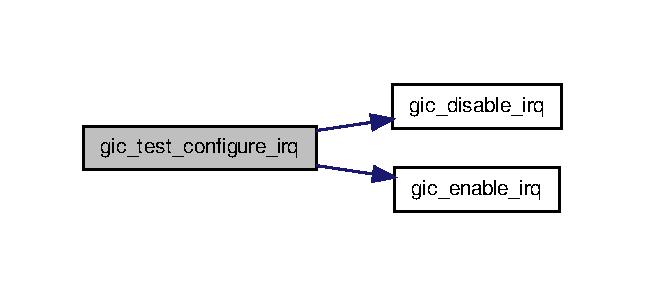
\includegraphics[width=310pt]{gic_8c_acbe5581611f81cd00b58cebeda222edf_cgraph}
\end{center}
\end{figure}


\hypertarget{gic_8c_aaee4d58fadbe09c39f45e8e114a4dd4d}{\index{gic.\-c@{gic.\-c}!gic\-\_\-test\-\_\-set\-\_\-irq\-\_\-handler@{gic\-\_\-test\-\_\-set\-\_\-irq\-\_\-handler}}
\index{gic\-\_\-test\-\_\-set\-\_\-irq\-\_\-handler@{gic\-\_\-test\-\_\-set\-\_\-irq\-\_\-handler}!gic.c@{gic.\-c}}
\subsubsection[{gic\-\_\-test\-\_\-set\-\_\-irq\-\_\-handler}]{\setlength{\rightskip}{0pt plus 5cm}{\bf hvmm\-\_\-status\-\_\-t} {\bf gic\-\_\-test\-\_\-set\-\_\-irq\-\_\-handler} (
\begin{DoxyParamCaption}
\item[{int}]{irq, }
\item[{{\bf gic\-\_\-irq\-\_\-handler\-\_\-t}}]{handler, }
\item[{void $\ast$}]{pdata}
\end{DoxyParamCaption}
)}}\label{gic_8c_aaee4d58fadbe09c39f45e8e114a4dd4d}


\-Definition at line 226 of file gic.\-c.


\begin{DoxyCode}
{
    hvmm_status_t result = HVMM_STATUS_BUSY;
    if ( irq < GIC_NUM_MAX_IRQS ) {
        _gic.handlers[irq] = handler;
        result = HVMM_STATUS_SUCCESS;
    }
    return result;
}
\end{DoxyCode}
\hypertarget{gic_8c_a608941cbc8ab5a657834d451f0368a6e}{\index{gic.\-c@{gic.\-c}!gic\-\_\-vgic\-\_\-baseaddr@{gic\-\_\-vgic\-\_\-baseaddr}}
\index{gic\-\_\-vgic\-\_\-baseaddr@{gic\-\_\-vgic\-\_\-baseaddr}!gic.c@{gic.\-c}}
\subsubsection[{gic\-\_\-vgic\-\_\-baseaddr}]{\setlength{\rightskip}{0pt plus 5cm}volatile {\bf uint32\-\_\-t}$\ast$ {\bf gic\-\_\-vgic\-\_\-baseaddr} (
\begin{DoxyParamCaption}
\item[{void}]{}
\end{DoxyParamCaption}
)}}\label{gic_8c_a608941cbc8ab5a657834d451f0368a6e}


\-Definition at line 236 of file gic.\-c.


\begin{DoxyCode}
{
    if ( _gic.initialized != GIC_SIGNATURE_INITIALIZED ) {
        HVMM_TRACE_ENTER();
        uart_print("gic: ERROR - not initialized\n\r");
        HVMM_TRACE_EXIT();
    }

    return _gic.ba_gich;
}
\end{DoxyCode}


\subsection{\-Variable \-Documentation}
\hypertarget{gic_8c_a812e13a3081e93998d02dcad7c12f64b}{\index{gic.\-c@{gic.\-c}!\-\_\-gic@{\-\_\-gic}}
\index{\-\_\-gic@{\-\_\-gic}!gic.c@{gic.\-c}}
\subsubsection[{\-\_\-gic}]{\setlength{\rightskip}{0pt plus 5cm}struct {\bf gic} {\bf \-\_\-gic}\hspace{0.3cm}{\ttfamily  \mbox{[}static\mbox{]}}}}\label{gic_8c_a812e13a3081e93998d02dcad7c12f64b}


\-Definition at line 44 of file gic.\-c.


\hypertarget{slotpirq_8c}{\section{gic/slotpirq.c \-File \-Reference}
\label{slotpirq_8c}\index{gic/slotpirq.\-c@{gic/slotpirq.\-c}}
}
{\ttfamily \#include $<$slotpirq.\-h$>$}\*
{\ttfamily \#include $<$k-\/hypervisor-\/config.\-h$>$}\*
{\ttfamily \#include $<$vgic.\-h$>$}\*
{\ttfamily \#include $<$log/print.\-h$>$}\*
\-Include dependency graph for slotpirq.\-c\-:
\nopagebreak
\begin{figure}[H]
\begin{center}
\leavevmode
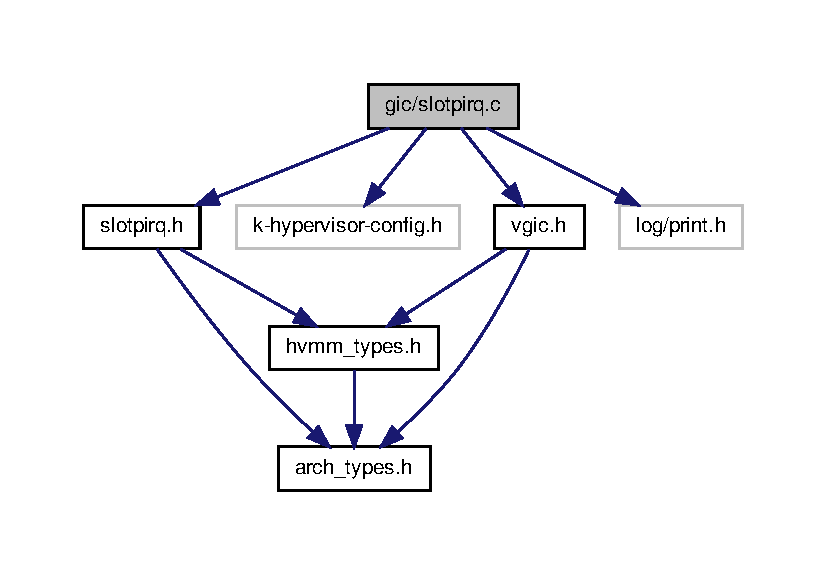
\includegraphics[width=350pt]{slotpirq_8c__incl}
\end{center}
\end{figure}
\subsection*{\-Functions}
\begin{DoxyCompactItemize}
\item 
void \hyperlink{slotpirq_8c_a01b3ab3099b2a5512a07cb42a389d84f}{slotpirq\-\_\-init} (void)
\item 
void \hyperlink{slotpirq_8c_aff1cbc822b730c991459afb793276fa6}{slotpirq\-\_\-set} (\hyperlink{hvmm__types_8h_af7e9bd0adfb7d10e7a7a0ee60a5f962c}{vmid\-\_\-t} vmid, \hyperlink{arch__types_8h_a435d1572bf3f880d55459d9805097f62}{uint32\-\_\-t} slot, \hyperlink{arch__types_8h_a435d1572bf3f880d55459d9805097f62}{uint32\-\_\-t} pirq)
\item 
\hyperlink{arch__types_8h_a435d1572bf3f880d55459d9805097f62}{uint32\-\_\-t} \hyperlink{slotpirq_8c_aa2a97d33b447c3cd1b54645301d67d06}{slotpirq\-\_\-get} (\hyperlink{hvmm__types_8h_af7e9bd0adfb7d10e7a7a0ee60a5f962c}{vmid\-\_\-t} vmid, \hyperlink{arch__types_8h_a435d1572bf3f880d55459d9805097f62}{uint32\-\_\-t} slot)
\item 
void \hyperlink{slotpirq_8c_a7796a08ae962d45173231eba6a4d6596}{slotpirq\-\_\-clear} (\hyperlink{hvmm__types_8h_af7e9bd0adfb7d10e7a7a0ee60a5f962c}{vmid\-\_\-t} vmid, \hyperlink{arch__types_8h_a435d1572bf3f880d55459d9805097f62}{uint32\-\_\-t} slot)
\item 
void \hyperlink{slotpirq_8c_aaad8058f8557950c87ce6e452e5a7223}{slotvirq\-\_\-set} (\hyperlink{hvmm__types_8h_af7e9bd0adfb7d10e7a7a0ee60a5f962c}{vmid\-\_\-t} vmid, \hyperlink{arch__types_8h_a435d1572bf3f880d55459d9805097f62}{uint32\-\_\-t} slot, \hyperlink{arch__types_8h_a435d1572bf3f880d55459d9805097f62}{uint32\-\_\-t} virq)
\item 
\hyperlink{arch__types_8h_a435d1572bf3f880d55459d9805097f62}{uint32\-\_\-t} \hyperlink{slotpirq_8c_a384b4abb370436f02ed5b937f3690a6c}{slotvirq\-\_\-getslot} (\hyperlink{hvmm__types_8h_af7e9bd0adfb7d10e7a7a0ee60a5f962c}{vmid\-\_\-t} vmid, \hyperlink{arch__types_8h_a435d1572bf3f880d55459d9805097f62}{uint32\-\_\-t} virq)
\item 
void \hyperlink{slotpirq_8c_afdec456416a60eafcb58f50c742d7de2}{slotvirq\-\_\-clear} (\hyperlink{hvmm__types_8h_af7e9bd0adfb7d10e7a7a0ee60a5f962c}{vmid\-\_\-t} vmid, \hyperlink{arch__types_8h_a435d1572bf3f880d55459d9805097f62}{uint32\-\_\-t} slot)
\end{DoxyCompactItemize}
\subsection*{\-Variables}
\begin{DoxyCompactItemize}
\item 
static \hyperlink{arch__types_8h_a435d1572bf3f880d55459d9805097f62}{uint32\-\_\-t} \hyperlink{slotpirq_8c_ae2bea4a5c120f4ea6fd57dc685c0c3a1}{\-\_\-guest\-\_\-pirqatslot} \mbox{[}\hyperlink{hyp__config_8h_a7fcfcbc766cea81a21e2d8aba3b54843}{\-N\-U\-M\-\_\-\-G\-U\-E\-S\-T\-S\-\_\-\-S\-T\-A\-T\-I\-C}\mbox{]}\mbox{[}\hyperlink{vgic_8h_abfdcf103267c36171a466d426374f51e}{\-V\-G\-I\-C\-\_\-\-N\-U\-M\-\_\-\-M\-A\-X\-\_\-\-S\-L\-O\-T\-S}\mbox{]}
\item 
static \hyperlink{arch__types_8h_a435d1572bf3f880d55459d9805097f62}{uint32\-\_\-t} \hyperlink{slotpirq_8c_a30a5e8d32abb941237bf77f56eb36e70}{\-\_\-guest\-\_\-virqatslot} \mbox{[}\hyperlink{hyp__config_8h_a7fcfcbc766cea81a21e2d8aba3b54843}{\-N\-U\-M\-\_\-\-G\-U\-E\-S\-T\-S\-\_\-\-S\-T\-A\-T\-I\-C}\mbox{]}\mbox{[}\hyperlink{vgic_8h_abfdcf103267c36171a466d426374f51e}{\-V\-G\-I\-C\-\_\-\-N\-U\-M\-\_\-\-M\-A\-X\-\_\-\-S\-L\-O\-T\-S}\mbox{]}
\end{DoxyCompactItemize}


\subsection{\-Function \-Documentation}
\hypertarget{slotpirq_8c_a7796a08ae962d45173231eba6a4d6596}{\index{slotpirq.\-c@{slotpirq.\-c}!slotpirq\-\_\-clear@{slotpirq\-\_\-clear}}
\index{slotpirq\-\_\-clear@{slotpirq\-\_\-clear}!slotpirq.c@{slotpirq.\-c}}
\subsubsection[{slotpirq\-\_\-clear}]{\setlength{\rightskip}{0pt plus 5cm}void {\bf slotpirq\-\_\-clear} (
\begin{DoxyParamCaption}
\item[{{\bf vmid\-\_\-t}}]{vmid, }
\item[{{\bf uint32\-\_\-t}}]{slot}
\end{DoxyParamCaption}
)}}\label{slotpirq_8c_a7796a08ae962d45173231eba6a4d6596}


\-Definition at line 40 of file slotpirq.\-c.


\begin{DoxyCode}
{
    slotpirq_set(vmid, slot, PIRQ_INVALID);
}
\end{DoxyCode}


\-Here is the call graph for this function\-:
\nopagebreak
\begin{figure}[H]
\begin{center}
\leavevmode
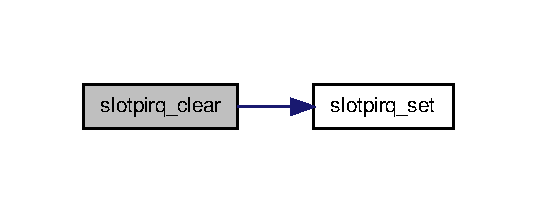
\includegraphics[width=258pt]{slotpirq_8c_a7796a08ae962d45173231eba6a4d6596_cgraph}
\end{center}
\end{figure}


\hypertarget{slotpirq_8c_aa2a97d33b447c3cd1b54645301d67d06}{\index{slotpirq.\-c@{slotpirq.\-c}!slotpirq\-\_\-get@{slotpirq\-\_\-get}}
\index{slotpirq\-\_\-get@{slotpirq\-\_\-get}!slotpirq.c@{slotpirq.\-c}}
\subsubsection[{slotpirq\-\_\-get}]{\setlength{\rightskip}{0pt plus 5cm}{\bf uint32\-\_\-t} {\bf slotpirq\-\_\-get} (
\begin{DoxyParamCaption}
\item[{{\bf vmid\-\_\-t}}]{vmid, }
\item[{{\bf uint32\-\_\-t}}]{slot}
\end{DoxyParamCaption}
)}}\label{slotpirq_8c_aa2a97d33b447c3cd1b54645301d67d06}


\-Definition at line 29 of file slotpirq.\-c.


\begin{DoxyCode}
{
    uint32_t pirq = PIRQ_INVALID;

    if ( vmid < NUM_GUESTS_STATIC ) {
        pirq = _guest_pirqatslot[vmid][slot];
        printh( "vgic: reading vmid:%d slot:%d pirq:%d\n", vmid, slot, pirq );
    }
    return pirq;
}
\end{DoxyCode}
\hypertarget{slotpirq_8c_a01b3ab3099b2a5512a07cb42a389d84f}{\index{slotpirq.\-c@{slotpirq.\-c}!slotpirq\-\_\-init@{slotpirq\-\_\-init}}
\index{slotpirq\-\_\-init@{slotpirq\-\_\-init}!slotpirq.c@{slotpirq.\-c}}
\subsubsection[{slotpirq\-\_\-init}]{\setlength{\rightskip}{0pt plus 5cm}void {\bf slotpirq\-\_\-init} (
\begin{DoxyParamCaption}
\item[{void}]{}
\end{DoxyParamCaption}
)}}\label{slotpirq_8c_a01b3ab3099b2a5512a07cb42a389d84f}


\-Definition at line 10 of file slotpirq.\-c.


\begin{DoxyCode}
{
    int i, j;
    for( i = 0; i < NUM_GUESTS_STATIC; i++ ) {
        for( j = 0; j < VGIC_NUM_MAX_SLOTS; j++ ) {
            _guest_pirqatslot[i][j] = PIRQ_INVALID;
            _guest_virqatslot[i][j] = VIRQ_INVALID;
        }
    }
}
\end{DoxyCode}
\hypertarget{slotpirq_8c_aff1cbc822b730c991459afb793276fa6}{\index{slotpirq.\-c@{slotpirq.\-c}!slotpirq\-\_\-set@{slotpirq\-\_\-set}}
\index{slotpirq\-\_\-set@{slotpirq\-\_\-set}!slotpirq.c@{slotpirq.\-c}}
\subsubsection[{slotpirq\-\_\-set}]{\setlength{\rightskip}{0pt plus 5cm}void {\bf slotpirq\-\_\-set} (
\begin{DoxyParamCaption}
\item[{{\bf vmid\-\_\-t}}]{vmid, }
\item[{{\bf uint32\-\_\-t}}]{slot, }
\item[{{\bf uint32\-\_\-t}}]{pirq}
\end{DoxyParamCaption}
)}}\label{slotpirq_8c_aff1cbc822b730c991459afb793276fa6}


\-Definition at line 21 of file slotpirq.\-c.


\begin{DoxyCode}
{
    if ( vmid < NUM_GUESTS_STATIC ) {
        printh( "vgic: setting vmid:%d slot:%d pirq:%d\n", vmid, slot, pirq );
        _guest_pirqatslot[vmid][slot] = pirq;
    }
}
\end{DoxyCode}
\hypertarget{slotpirq_8c_afdec456416a60eafcb58f50c742d7de2}{\index{slotpirq.\-c@{slotpirq.\-c}!slotvirq\-\_\-clear@{slotvirq\-\_\-clear}}
\index{slotvirq\-\_\-clear@{slotvirq\-\_\-clear}!slotpirq.c@{slotpirq.\-c}}
\subsubsection[{slotvirq\-\_\-clear}]{\setlength{\rightskip}{0pt plus 5cm}void {\bf slotvirq\-\_\-clear} (
\begin{DoxyParamCaption}
\item[{{\bf vmid\-\_\-t}}]{vmid, }
\item[{{\bf uint32\-\_\-t}}]{slot}
\end{DoxyParamCaption}
)}}\label{slotpirq_8c_afdec456416a60eafcb58f50c742d7de2}


\-Definition at line 72 of file slotpirq.\-c.


\begin{DoxyCode}
{
    slotvirq_set(vmid, slot, VIRQ_INVALID);
}
\end{DoxyCode}


\-Here is the call graph for this function\-:
\nopagebreak
\begin{figure}[H]
\begin{center}
\leavevmode
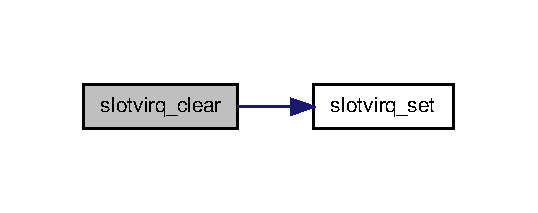
\includegraphics[width=258pt]{slotpirq_8c_afdec456416a60eafcb58f50c742d7de2_cgraph}
\end{center}
\end{figure}


\hypertarget{slotpirq_8c_a384b4abb370436f02ed5b937f3690a6c}{\index{slotpirq.\-c@{slotpirq.\-c}!slotvirq\-\_\-getslot@{slotvirq\-\_\-getslot}}
\index{slotvirq\-\_\-getslot@{slotvirq\-\_\-getslot}!slotpirq.c@{slotpirq.\-c}}
\subsubsection[{slotvirq\-\_\-getslot}]{\setlength{\rightskip}{0pt plus 5cm}{\bf uint32\-\_\-t} {\bf slotvirq\-\_\-getslot} (
\begin{DoxyParamCaption}
\item[{{\bf vmid\-\_\-t}}]{vmid, }
\item[{{\bf uint32\-\_\-t}}]{virq}
\end{DoxyParamCaption}
)}}\label{slotpirq_8c_a384b4abb370436f02ed5b937f3690a6c}


\-Definition at line 55 of file slotpirq.\-c.


\begin{DoxyCode}
{
    uint32_t slot = SLOT_INVALID;
    int i;

    if ( vmid < NUM_GUESTS_STATIC ) {
        for ( i = 0; i < VGIC_NUM_MAX_SLOTS; i++ ) {
            if ( _guest_virqatslot[vmid][i] == virq ) {
                slot = i;
                printh( "vgic: reading vmid:%d slot:%d virq:%d\n", vmid, slot, 
      virq );
                break;
            }
        }
    }
    return slot;
}
\end{DoxyCode}
\hypertarget{slotpirq_8c_aaad8058f8557950c87ce6e452e5a7223}{\index{slotpirq.\-c@{slotpirq.\-c}!slotvirq\-\_\-set@{slotvirq\-\_\-set}}
\index{slotvirq\-\_\-set@{slotvirq\-\_\-set}!slotpirq.c@{slotpirq.\-c}}
\subsubsection[{slotvirq\-\_\-set}]{\setlength{\rightskip}{0pt plus 5cm}void {\bf slotvirq\-\_\-set} (
\begin{DoxyParamCaption}
\item[{{\bf vmid\-\_\-t}}]{vmid, }
\item[{{\bf uint32\-\_\-t}}]{slot, }
\item[{{\bf uint32\-\_\-t}}]{virq}
\end{DoxyParamCaption}
)}}\label{slotpirq_8c_aaad8058f8557950c87ce6e452e5a7223}


\-Definition at line 45 of file slotpirq.\-c.


\begin{DoxyCode}
{
    if ( vmid < NUM_GUESTS_STATIC ) {
        printh( "vgic: setting vmid:%d slot:%d virq:%d\n", vmid, slot, virq );
        _guest_virqatslot[vmid][slot] = virq;
    } else {
        printh( "vgic: not setting invalid vmid:%d slot:%d virq:%d\n", vmid, 
      slot, virq );
    }
}
\end{DoxyCode}


\subsection{\-Variable \-Documentation}
\hypertarget{slotpirq_8c_ae2bea4a5c120f4ea6fd57dc685c0c3a1}{\index{slotpirq.\-c@{slotpirq.\-c}!\-\_\-guest\-\_\-pirqatslot@{\-\_\-guest\-\_\-pirqatslot}}
\index{\-\_\-guest\-\_\-pirqatslot@{\-\_\-guest\-\_\-pirqatslot}!slotpirq.c@{slotpirq.\-c}}
\subsubsection[{\-\_\-guest\-\_\-pirqatslot}]{\setlength{\rightskip}{0pt plus 5cm}{\bf uint32\-\_\-t} {\bf \-\_\-guest\-\_\-pirqatslot}\mbox{[}{\bf \-N\-U\-M\-\_\-\-G\-U\-E\-S\-T\-S\-\_\-\-S\-T\-A\-T\-I\-C}\mbox{]}\mbox{[}{\bf \-V\-G\-I\-C\-\_\-\-N\-U\-M\-\_\-\-M\-A\-X\-\_\-\-S\-L\-O\-T\-S}\mbox{]}\hspace{0.3cm}{\ttfamily  \mbox{[}static\mbox{]}}}}\label{slotpirq_8c_ae2bea4a5c120f4ea6fd57dc685c0c3a1}


\-Definition at line 7 of file slotpirq.\-c.

\hypertarget{slotpirq_8c_a30a5e8d32abb941237bf77f56eb36e70}{\index{slotpirq.\-c@{slotpirq.\-c}!\-\_\-guest\-\_\-virqatslot@{\-\_\-guest\-\_\-virqatslot}}
\index{\-\_\-guest\-\_\-virqatslot@{\-\_\-guest\-\_\-virqatslot}!slotpirq.c@{slotpirq.\-c}}
\subsubsection[{\-\_\-guest\-\_\-virqatslot}]{\setlength{\rightskip}{0pt plus 5cm}{\bf uint32\-\_\-t} {\bf \-\_\-guest\-\_\-virqatslot}\mbox{[}{\bf \-N\-U\-M\-\_\-\-G\-U\-E\-S\-T\-S\-\_\-\-S\-T\-A\-T\-I\-C}\mbox{]}\mbox{[}{\bf \-V\-G\-I\-C\-\_\-\-N\-U\-M\-\_\-\-M\-A\-X\-\_\-\-S\-L\-O\-T\-S}\mbox{]}\hspace{0.3cm}{\ttfamily  \mbox{[}static\mbox{]}}}}\label{slotpirq_8c_a30a5e8d32abb941237bf77f56eb36e70}


\-Definition at line 8 of file slotpirq.\-c.


\hypertarget{vgic_8c}{\section{gic/vgic.c \-File \-Reference}
\label{vgic_8c}\index{gic/vgic.\-c@{gic/vgic.\-c}}
}
{\ttfamily \#include $<$vgic.\-h$>$}\*
{\ttfamily \#include $<$hvmm\-\_\-trace.\-h$>$}\*
{\ttfamily \#include $<$armv7\-\_\-p15.\-h$>$}\*
{\ttfamily \#include $<$gic.\-h$>$}\*
{\ttfamily \#include $<$gic\-\_\-regs.\-h$>$}\*
{\ttfamily \#include $<$slotpirq.\-h$>$}\*
{\ttfamily \#include $<$context.\-h$>$}\*
{\ttfamily \#include $<$k-\/hypervisor-\/config.\-h$>$}\*
{\ttfamily \#include $<$asm-\/arm\-\_\-inline.\-h$>$}\*
{\ttfamily \#include $<$log/print.\-h$>$}\*
\-Include dependency graph for vgic.\-c\-:
\nopagebreak
\begin{figure}[H]
\begin{center}
\leavevmode
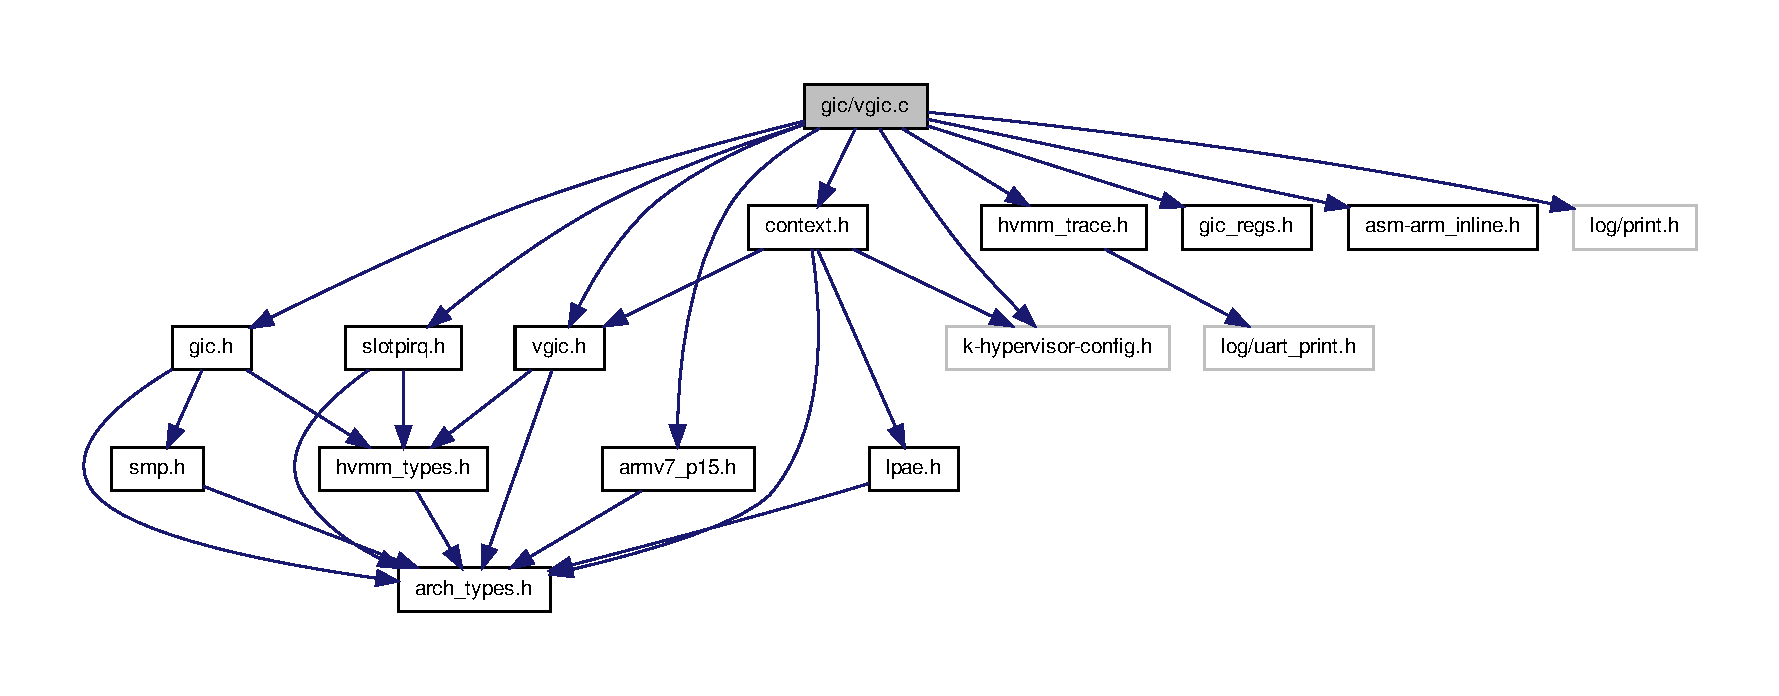
\includegraphics[width=350pt]{vgic_8c__incl}
\end{center}
\end{figure}
\subsection*{\-Data \-Structures}
\begin{DoxyCompactItemize}
\item 
struct \hyperlink{structvgic}{vgic}
\end{DoxyCompactItemize}
\subsection*{\-Defines}
\begin{DoxyCompactItemize}
\item 
\#define \hyperlink{vgic_8c_a526061ee0fe28ae7bf22f0ba3c4a0d4c}{\-\_\-\-\_\-\-V\-G\-I\-C\-\_\-\-D\-I\-S\-A\-B\-L\-E\-\_\-\-T\-R\-A\-C\-E\-\_\-\-\_\-}
\item 
\#define \hyperlink{vgic_8c_a7b7b6f67ad514ac2101b96175a9ec29f}{\-V\-G\-I\-C\-\_\-\-S\-I\-M\-U\-L\-A\-T\-E\-\_\-\-H\-W\-V\-I\-R\-Q}
\item 
\#define \hyperlink{vgic_8c_a75c7cfc017c76385de9ae23d3a003351}{\-V\-G\-I\-C\-\_\-\-M\-A\-I\-N\-T\-E\-N\-A\-N\-C\-E\-\_\-\-I\-N\-T\-E\-R\-R\-U\-P\-T\-\_\-\-I\-R\-Q}~25
\item 
\#define \hyperlink{vgic_8c_a07d069eab0ef3cee053462d7983e58fc}{\-V\-G\-I\-C\-\_\-\-M\-A\-X\-\_\-\-L\-I\-S\-T\-R\-E\-G\-I\-S\-T\-E\-R\-S}~\hyperlink{vgic_8h_abfdcf103267c36171a466d426374f51e}{\-V\-G\-I\-C\-\_\-\-N\-U\-M\-\_\-\-M\-A\-X\-\_\-\-S\-L\-O\-T\-S}
\item 
\#define \hyperlink{vgic_8c_ab069326a104b1d5b811b25aa42402dc3}{\-V\-G\-I\-C\-\_\-\-S\-I\-G\-N\-A\-T\-U\-R\-E\-\_\-\-I\-N\-I\-T\-I\-A\-L\-I\-Z\-E\-D}~0x45108\-E\-A\-D
\item 
\#define \hyperlink{vgic_8c_ab8ea3db7e1235ef68503d53d964e35f8}{\-V\-G\-I\-C\-\_\-\-R\-E\-A\-D\-Y}()~(\-\_\-vgic.\-initialized == \hyperlink{vgic_8c_ab069326a104b1d5b811b25aa42402dc3}{\-V\-G\-I\-C\-\_\-\-S\-I\-G\-N\-A\-T\-U\-R\-E\-\_\-\-I\-N\-I\-T\-I\-A\-L\-I\-Z\-E\-D})
\end{DoxyCompactItemize}
\subsection*{\-Functions}
\begin{DoxyCompactItemize}
\item 
\hyperlink{hvmm__types_8h_a39d593b2c97852f566d7472b76ab7ba2}{hvmm\-\_\-status\-\_\-t} \hyperlink{vgic_8c_ae71b0763ed8149031b08ad13d8d687cb}{vgic\-\_\-injection\-\_\-enable} (\hyperlink{arch__types_8h_aba7bc1797add20fe3efdf37ced1182c5}{uint8\-\_\-t} enable)
\item 
static \hyperlink{arch__types_8h_a435d1572bf3f880d55459d9805097f62}{uint32\-\_\-t} \hyperlink{vgic_8c_aab31fc8d2c44ebb938b78cfb1f7c975f}{vgic\-\_\-find\-\_\-free\-\_\-slot} (void)
\item 
static \hyperlink{arch__types_8h_a435d1572bf3f880d55459d9805097f62}{uint32\-\_\-t} \hyperlink{vgic_8c_ac1d43326139a3717d69ce1f876cd221c}{vgic\-\_\-is\-\_\-free\-\_\-slot} (\hyperlink{arch__types_8h_a435d1572bf3f880d55459d9805097f62}{uint32\-\_\-t} slot)
\item 
static void \hyperlink{vgic_8c_aea2435da2d73a22a35b601508d6ea6da}{\-\_\-vgic\-\_\-dump\-\_\-status} (void)
\item 
static void \hyperlink{vgic_8c_abfca2f5be8dfbb355800d70dbda23b5e}{\-\_\-vgic\-\_\-dump\-\_\-regs} (void)
\item 
static void \hyperlink{vgic_8c_a8d083941ad4202604d2ec7161c8f6409}{\-\_\-vgic\-\_\-isr\-\_\-maintenance\-\_\-irq} (int irq, void $\ast$pregs, void $\ast$pdata)
\item 
\hyperlink{hvmm__types_8h_a39d593b2c97852f566d7472b76ab7ba2}{hvmm\-\_\-status\-\_\-t} \hyperlink{vgic_8c_a4cf554520738a7934bc4e6917853330c}{vgic\-\_\-enable} (\hyperlink{arch__types_8h_aba7bc1797add20fe3efdf37ced1182c5}{uint8\-\_\-t} enable)
\item 
\hyperlink{arch__types_8h_a435d1572bf3f880d55459d9805097f62}{uint32\-\_\-t} \hyperlink{vgic_8c_a6fb239504a0f9b77f78ca1f75318f78f}{vgic\-\_\-inject\-\_\-virq} (\hyperlink{arch__types_8h_a435d1572bf3f880d55459d9805097f62}{uint32\-\_\-t} virq, \hyperlink{arch__types_8h_a435d1572bf3f880d55459d9805097f62}{uint32\-\_\-t} slot, \hyperlink{vgic_8h_a7028e35242589b61104f1b59574e43df}{virq\-\_\-state\-\_\-t} state, \hyperlink{arch__types_8h_a435d1572bf3f880d55459d9805097f62}{uint32\-\_\-t} priority, \hyperlink{arch__types_8h_aba7bc1797add20fe3efdf37ced1182c5}{uint8\-\_\-t} hw, \hyperlink{arch__types_8h_a435d1572bf3f880d55459d9805097f62}{uint32\-\_\-t} physrc, \hyperlink{arch__types_8h_aba7bc1797add20fe3efdf37ced1182c5}{uint8\-\_\-t} maintenance)
\item 
\hyperlink{arch__types_8h_a435d1572bf3f880d55459d9805097f62}{uint32\-\_\-t} \hyperlink{vgic_8c_a93b048baf04857249e2ba3c24a82407f}{vgic\-\_\-inject\-\_\-virq\-\_\-hw} (\hyperlink{arch__types_8h_a435d1572bf3f880d55459d9805097f62}{uint32\-\_\-t} virq, \hyperlink{vgic_8h_a7028e35242589b61104f1b59574e43df}{virq\-\_\-state\-\_\-t} state, \hyperlink{arch__types_8h_a435d1572bf3f880d55459d9805097f62}{uint32\-\_\-t} priority, \hyperlink{arch__types_8h_a435d1572bf3f880d55459d9805097f62}{uint32\-\_\-t} pirq)
\item 
\hyperlink{arch__types_8h_a435d1572bf3f880d55459d9805097f62}{uint32\-\_\-t} \hyperlink{vgic_8c_a6fa5c258f61efb0140f0b85175d25ff5}{vgic\-\_\-inject\-\_\-virq\-\_\-sw} (\hyperlink{arch__types_8h_a435d1572bf3f880d55459d9805097f62}{uint32\-\_\-t} virq, \hyperlink{vgic_8h_a7028e35242589b61104f1b59574e43df}{virq\-\_\-state\-\_\-t} state, \hyperlink{arch__types_8h_a435d1572bf3f880d55459d9805097f62}{uint32\-\_\-t} priority, \hyperlink{arch__types_8h_a435d1572bf3f880d55459d9805097f62}{uint32\-\_\-t} cpuid, \hyperlink{arch__types_8h_aba7bc1797add20fe3efdf37ced1182c5}{uint8\-\_\-t} maintenance)
\item 
\hyperlink{hvmm__types_8h_a39d593b2c97852f566d7472b76ab7ba2}{hvmm\-\_\-status\-\_\-t} \hyperlink{vgic_8c_a896fa453c39e4d42fa37483b07c7d307}{vgic\-\_\-maintenance\-\_\-irq\-\_\-enable} (\hyperlink{arch__types_8h_aba7bc1797add20fe3efdf37ced1182c5}{uint8\-\_\-t} enable)
\item 
static \hyperlink{arch__types_8h_aaa5d1cd013383c889537491c3cfd9aad}{uint64\-\_\-t} \hyperlink{vgic_8c_a66eca59dda59d2529191ca0c23094fc8}{\-\_\-vgic\-\_\-valid\-\_\-lr\-\_\-mask} (\hyperlink{arch__types_8h_a435d1572bf3f880d55459d9805097f62}{uint32\-\_\-t} num\-\_\-lr)
\item 
\hyperlink{hvmm__types_8h_a39d593b2c97852f566d7472b76ab7ba2}{hvmm\-\_\-status\-\_\-t} \hyperlink{vgic_8c_a2302c75a54486f179f199997b4a268b3}{vgic\-\_\-setcallback\-\_\-virq\-\_\-flush} (void($\ast$callback)(\hyperlink{hvmm__types_8h_af7e9bd0adfb7d10e7a7a0ee60a5f962c}{vmid\-\_\-t} vmid))
\item 
\hyperlink{hvmm__types_8h_a39d593b2c97852f566d7472b76ab7ba2}{hvmm\-\_\-status\-\_\-t} \hyperlink{vgic_8c_a2e0db8f93d8d6a61d737de34aeeed516}{vgic\-\_\-init} (void)
\item 
\hyperlink{hvmm__types_8h_a39d593b2c97852f566d7472b76ab7ba2}{hvmm\-\_\-status\-\_\-t} \hyperlink{vgic_8c_ac901a925af53a53bf1840d9be9acd2e0}{vgic\-\_\-init\-\_\-status} (struct \hyperlink{structvgic__status}{vgic\-\_\-status} $\ast$status, \hyperlink{hvmm__types_8h_af7e9bd0adfb7d10e7a7a0ee60a5f962c}{vmid\-\_\-t} vmid)
\item 
\hyperlink{hvmm__types_8h_a39d593b2c97852f566d7472b76ab7ba2}{hvmm\-\_\-status\-\_\-t} \hyperlink{vgic_8c_aebad7b956b2c36d2bbe7acdbe333ae8a}{vgic\-\_\-save\-\_\-status} (struct \hyperlink{structvgic__status}{vgic\-\_\-status} $\ast$status, \hyperlink{hvmm__types_8h_af7e9bd0adfb7d10e7a7a0ee60a5f962c}{vmid\-\_\-t} vmid)
\item 
\hyperlink{hvmm__types_8h_a39d593b2c97852f566d7472b76ab7ba2}{hvmm\-\_\-status\-\_\-t} \hyperlink{vgic_8c_a70332a1790f88fbcb1a4c7014e6b6a02}{vgic\-\_\-restore\-\_\-status} (struct \hyperlink{structvgic__status}{vgic\-\_\-status} $\ast$status, \hyperlink{hvmm__types_8h_af7e9bd0adfb7d10e7a7a0ee60a5f962c}{vmid\-\_\-t} vmid)
\item 
\hyperlink{hvmm__types_8h_a39d593b2c97852f566d7472b76ab7ba2}{hvmm\-\_\-status\-\_\-t} \hyperlink{vgic_8c_acb00c28d2618d3581a7d26f8e265ccb8}{vgic\-\_\-flush\-\_\-virqs} (\hyperlink{hvmm__types_8h_af7e9bd0adfb7d10e7a7a0ee60a5f962c}{vmid\-\_\-t} vmid)
\end{DoxyCompactItemize}
\subsection*{\-Variables}
\begin{DoxyCompactItemize}
\item 
static struct \hyperlink{structvgic}{vgic} \hyperlink{vgic_8c_a5191716b54330506bb98f687550f2812}{\-\_\-vgic}
\item 
static void($\ast$ \hyperlink{vgic_8c_a91dbbb7f0fc3b51b2cc9482aaa444d39}{\-\_\-cb\-\_\-virq\-\_\-flush} )(\hyperlink{hvmm__types_8h_af7e9bd0adfb7d10e7a7a0ee60a5f962c}{vmid\-\_\-t} vmid)=0
\end{DoxyCompactItemize}


\subsection{\-Define \-Documentation}
\hypertarget{vgic_8c_a526061ee0fe28ae7bf22f0ba3c4a0d4c}{\index{vgic.\-c@{vgic.\-c}!\-\_\-\-\_\-\-V\-G\-I\-C\-\_\-\-D\-I\-S\-A\-B\-L\-E\-\_\-\-T\-R\-A\-C\-E\-\_\-\-\_\-@{\-\_\-\-\_\-\-V\-G\-I\-C\-\_\-\-D\-I\-S\-A\-B\-L\-E\-\_\-\-T\-R\-A\-C\-E\-\_\-\-\_\-}}
\index{\-\_\-\-\_\-\-V\-G\-I\-C\-\_\-\-D\-I\-S\-A\-B\-L\-E\-\_\-\-T\-R\-A\-C\-E\-\_\-\-\_\-@{\-\_\-\-\_\-\-V\-G\-I\-C\-\_\-\-D\-I\-S\-A\-B\-L\-E\-\_\-\-T\-R\-A\-C\-E\-\_\-\-\_\-}!vgic.c@{vgic.\-c}}
\subsubsection[{\-\_\-\-\_\-\-V\-G\-I\-C\-\_\-\-D\-I\-S\-A\-B\-L\-E\-\_\-\-T\-R\-A\-C\-E\-\_\-\-\_\-}]{\setlength{\rightskip}{0pt plus 5cm}\#define {\bf \-\_\-\-\_\-\-V\-G\-I\-C\-\_\-\-D\-I\-S\-A\-B\-L\-E\-\_\-\-T\-R\-A\-C\-E\-\_\-\-\_\-}}}\label{vgic_8c_a526061ee0fe28ae7bf22f0ba3c4a0d4c}


\-Definition at line 14 of file vgic.\-c.

\hypertarget{vgic_8c_a75c7cfc017c76385de9ae23d3a003351}{\index{vgic.\-c@{vgic.\-c}!\-V\-G\-I\-C\-\_\-\-M\-A\-I\-N\-T\-E\-N\-A\-N\-C\-E\-\_\-\-I\-N\-T\-E\-R\-R\-U\-P\-T\-\_\-\-I\-R\-Q@{\-V\-G\-I\-C\-\_\-\-M\-A\-I\-N\-T\-E\-N\-A\-N\-C\-E\-\_\-\-I\-N\-T\-E\-R\-R\-U\-P\-T\-\_\-\-I\-R\-Q}}
\index{\-V\-G\-I\-C\-\_\-\-M\-A\-I\-N\-T\-E\-N\-A\-N\-C\-E\-\_\-\-I\-N\-T\-E\-R\-R\-U\-P\-T\-\_\-\-I\-R\-Q@{\-V\-G\-I\-C\-\_\-\-M\-A\-I\-N\-T\-E\-N\-A\-N\-C\-E\-\_\-\-I\-N\-T\-E\-R\-R\-U\-P\-T\-\_\-\-I\-R\-Q}!vgic.c@{vgic.\-c}}
\subsubsection[{\-V\-G\-I\-C\-\_\-\-M\-A\-I\-N\-T\-E\-N\-A\-N\-C\-E\-\_\-\-I\-N\-T\-E\-R\-R\-U\-P\-T\-\_\-\-I\-R\-Q}]{\setlength{\rightskip}{0pt plus 5cm}\#define {\bf \-V\-G\-I\-C\-\_\-\-M\-A\-I\-N\-T\-E\-N\-A\-N\-C\-E\-\_\-\-I\-N\-T\-E\-R\-R\-U\-P\-T\-\_\-\-I\-R\-Q}~25}}\label{vgic_8c_a75c7cfc017c76385de9ae23d3a003351}


\-Definition at line 29 of file vgic.\-c.

\hypertarget{vgic_8c_a07d069eab0ef3cee053462d7983e58fc}{\index{vgic.\-c@{vgic.\-c}!\-V\-G\-I\-C\-\_\-\-M\-A\-X\-\_\-\-L\-I\-S\-T\-R\-E\-G\-I\-S\-T\-E\-R\-S@{\-V\-G\-I\-C\-\_\-\-M\-A\-X\-\_\-\-L\-I\-S\-T\-R\-E\-G\-I\-S\-T\-E\-R\-S}}
\index{\-V\-G\-I\-C\-\_\-\-M\-A\-X\-\_\-\-L\-I\-S\-T\-R\-E\-G\-I\-S\-T\-E\-R\-S@{\-V\-G\-I\-C\-\_\-\-M\-A\-X\-\_\-\-L\-I\-S\-T\-R\-E\-G\-I\-S\-T\-E\-R\-S}!vgic.c@{vgic.\-c}}
\subsubsection[{\-V\-G\-I\-C\-\_\-\-M\-A\-X\-\_\-\-L\-I\-S\-T\-R\-E\-G\-I\-S\-T\-E\-R\-S}]{\setlength{\rightskip}{0pt plus 5cm}\#define {\bf \-V\-G\-I\-C\-\_\-\-M\-A\-X\-\_\-\-L\-I\-S\-T\-R\-E\-G\-I\-S\-T\-E\-R\-S}~{\bf \-V\-G\-I\-C\-\_\-\-N\-U\-M\-\_\-\-M\-A\-X\-\_\-\-S\-L\-O\-T\-S}}}\label{vgic_8c_a07d069eab0ef3cee053462d7983e58fc}


\-Definition at line 31 of file vgic.\-c.

\hypertarget{vgic_8c_ab8ea3db7e1235ef68503d53d964e35f8}{\index{vgic.\-c@{vgic.\-c}!\-V\-G\-I\-C\-\_\-\-R\-E\-A\-D\-Y@{\-V\-G\-I\-C\-\_\-\-R\-E\-A\-D\-Y}}
\index{\-V\-G\-I\-C\-\_\-\-R\-E\-A\-D\-Y@{\-V\-G\-I\-C\-\_\-\-R\-E\-A\-D\-Y}!vgic.c@{vgic.\-c}}
\subsubsection[{\-V\-G\-I\-C\-\_\-\-R\-E\-A\-D\-Y}]{\setlength{\rightskip}{0pt plus 5cm}\#define {\bf \-V\-G\-I\-C\-\_\-\-R\-E\-A\-D\-Y}(
\begin{DoxyParamCaption}
{}
\end{DoxyParamCaption}
)~(\-\_\-vgic.\-initialized == {\bf \-V\-G\-I\-C\-\_\-\-S\-I\-G\-N\-A\-T\-U\-R\-E\-\_\-\-I\-N\-I\-T\-I\-A\-L\-I\-Z\-E\-D})}}\label{vgic_8c_ab8ea3db7e1235ef68503d53d964e35f8}


\-Definition at line 33 of file vgic.\-c.

\hypertarget{vgic_8c_ab069326a104b1d5b811b25aa42402dc3}{\index{vgic.\-c@{vgic.\-c}!\-V\-G\-I\-C\-\_\-\-S\-I\-G\-N\-A\-T\-U\-R\-E\-\_\-\-I\-N\-I\-T\-I\-A\-L\-I\-Z\-E\-D@{\-V\-G\-I\-C\-\_\-\-S\-I\-G\-N\-A\-T\-U\-R\-E\-\_\-\-I\-N\-I\-T\-I\-A\-L\-I\-Z\-E\-D}}
\index{\-V\-G\-I\-C\-\_\-\-S\-I\-G\-N\-A\-T\-U\-R\-E\-\_\-\-I\-N\-I\-T\-I\-A\-L\-I\-Z\-E\-D@{\-V\-G\-I\-C\-\_\-\-S\-I\-G\-N\-A\-T\-U\-R\-E\-\_\-\-I\-N\-I\-T\-I\-A\-L\-I\-Z\-E\-D}!vgic.c@{vgic.\-c}}
\subsubsection[{\-V\-G\-I\-C\-\_\-\-S\-I\-G\-N\-A\-T\-U\-R\-E\-\_\-\-I\-N\-I\-T\-I\-A\-L\-I\-Z\-E\-D}]{\setlength{\rightskip}{0pt plus 5cm}\#define {\bf \-V\-G\-I\-C\-\_\-\-S\-I\-G\-N\-A\-T\-U\-R\-E\-\_\-\-I\-N\-I\-T\-I\-A\-L\-I\-Z\-E\-D}~0x45108\-E\-A\-D}}\label{vgic_8c_ab069326a104b1d5b811b25aa42402dc3}


\-Definition at line 32 of file vgic.\-c.

\hypertarget{vgic_8c_a7b7b6f67ad514ac2101b96175a9ec29f}{\index{vgic.\-c@{vgic.\-c}!\-V\-G\-I\-C\-\_\-\-S\-I\-M\-U\-L\-A\-T\-E\-\_\-\-H\-W\-V\-I\-R\-Q@{\-V\-G\-I\-C\-\_\-\-S\-I\-M\-U\-L\-A\-T\-E\-\_\-\-H\-W\-V\-I\-R\-Q}}
\index{\-V\-G\-I\-C\-\_\-\-S\-I\-M\-U\-L\-A\-T\-E\-\_\-\-H\-W\-V\-I\-R\-Q@{\-V\-G\-I\-C\-\_\-\-S\-I\-M\-U\-L\-A\-T\-E\-\_\-\-H\-W\-V\-I\-R\-Q}!vgic.c@{vgic.\-c}}
\subsubsection[{\-V\-G\-I\-C\-\_\-\-S\-I\-M\-U\-L\-A\-T\-E\-\_\-\-H\-W\-V\-I\-R\-Q}]{\setlength{\rightskip}{0pt plus 5cm}\#define {\bf \-V\-G\-I\-C\-\_\-\-S\-I\-M\-U\-L\-A\-T\-E\-\_\-\-H\-W\-V\-I\-R\-Q}}}\label{vgic_8c_a7b7b6f67ad514ac2101b96175a9ec29f}


\-Definition at line 15 of file vgic.\-c.



\subsection{\-Function \-Documentation}
\hypertarget{vgic_8c_abfca2f5be8dfbb355800d70dbda23b5e}{\index{vgic.\-c@{vgic.\-c}!\-\_\-vgic\-\_\-dump\-\_\-regs@{\-\_\-vgic\-\_\-dump\-\_\-regs}}
\index{\-\_\-vgic\-\_\-dump\-\_\-regs@{\-\_\-vgic\-\_\-dump\-\_\-regs}!vgic.c@{vgic.\-c}}
\subsubsection[{\-\_\-vgic\-\_\-dump\-\_\-regs}]{\setlength{\rightskip}{0pt plus 5cm}static void {\bf \-\_\-vgic\-\_\-dump\-\_\-regs} (
\begin{DoxyParamCaption}
\item[{void}]{}
\end{DoxyParamCaption}
)\hspace{0.3cm}{\ttfamily  \mbox{[}static\mbox{]}}}}\label{vgic_8c_abfca2f5be8dfbb355800d70dbda23b5e}


\-Definition at line 162 of file vgic.\-c.


\begin{DoxyCode}
{
#ifndef __VGIC_DISABLE_TRACE__
    /*
     * HCR * VTR * VMCR * MISR * EISR0 * EISR1 * ELSR0 * ELSR1 * APR * LR0~n
     */
    int i;
    HVMM_TRACE_ENTER();

    uart_print("  hcr:"); uart_print_hex32( _vgic.base[GICH_HCR] ); uart_print(
      "\n\r");
    uart_print("  vtr:"); uart_print_hex32( _vgic.base[GICH_VTR] ); uart_print(
      "\n\r");
    uart_print(" vmcr:"); uart_print_hex32( _vgic.base[GICH_VMCR] ); uart_print
      ("\n\r");
    uart_print(" misr:"); uart_print_hex32( _vgic.base[GICH_MISR] ); uart_print
      ("\n\r");
    uart_print("eisr0:"); uart_print_hex32( _vgic.base[GICH_EISR0] ); 
      uart_print("\n\r");
    uart_print("eisr1:"); uart_print_hex32( _vgic.base[GICH_EISR1] ); 
      uart_print("\n\r");
    uart_print("elsr0:"); uart_print_hex32( _vgic.base[GICH_ELSR0] ); 
      uart_print("\n\r");
    uart_print("elsr1:"); uart_print_hex32( _vgic.base[GICH_ELSR1] ); 
      uart_print("\n\r");
    uart_print("  apr:"); uart_print_hex32( _vgic.base[GICH_APR] ); uart_print(
      "\n\r");

    uart_print("   LR:\n\r"); 
    for( i = 0; i < _vgic.num_lr; i++ ) {
        if ( vgic_is_free_slot(i) != i ) {
            uart_print_hex32( _vgic.base[GICH_LR + i] ); uart_print(" - "); 
      uart_print_hex32(i); uart_print("\n\r");
        }
    }

    HVMM_TRACE_EXIT();
#endif
}
\end{DoxyCode}


\-Here is the call graph for this function\-:
\nopagebreak
\begin{figure}[H]
\begin{center}
\leavevmode
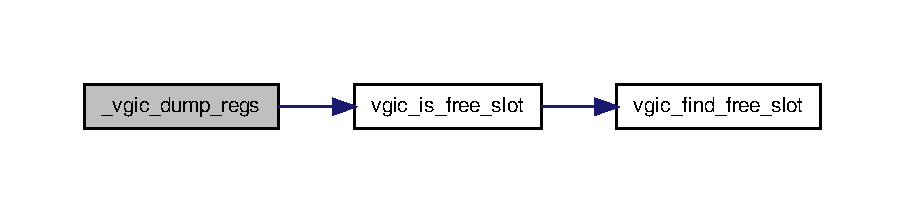
\includegraphics[width=350pt]{vgic_8c_abfca2f5be8dfbb355800d70dbda23b5e_cgraph}
\end{center}
\end{figure}


\hypertarget{vgic_8c_aea2435da2d73a22a35b601508d6ea6da}{\index{vgic.\-c@{vgic.\-c}!\-\_\-vgic\-\_\-dump\-\_\-status@{\-\_\-vgic\-\_\-dump\-\_\-status}}
\index{\-\_\-vgic\-\_\-dump\-\_\-status@{\-\_\-vgic\-\_\-dump\-\_\-status}!vgic.c@{vgic.\-c}}
\subsubsection[{\-\_\-vgic\-\_\-dump\-\_\-status}]{\setlength{\rightskip}{0pt plus 5cm}static void {\bf \-\_\-vgic\-\_\-dump\-\_\-status} (
\begin{DoxyParamCaption}
\item[{void}]{}
\end{DoxyParamCaption}
)\hspace{0.3cm}{\ttfamily  \mbox{[}static\mbox{]}}}}\label{vgic_8c_aea2435da2d73a22a35b601508d6ea6da}


\-Definition at line 133 of file vgic.\-c.


\begin{DoxyCode}
{
    /*
     * === VGIC Status Summary ===
     * Initialized: Yes
     * Num ListRegs: n
     * Hypervisor Control
     *  - Enabled: Yes
     *  - EOICount: 
     *  - Underflow:
     *  - LRENPIE:
     *  - NPIE:
     *  - VGrp0EIE:
     *  - VGrp0DIE:
     *  - VGrp1EIE:
     *  - VGrp1DIE:
     * VGIC Type
     *  - ListRegs:
     *  - PREbits:
     *  - PRIbits:
     * Virtual Machine Control
     *  - 
     */
    uart_print("=== VGIC Status ===\n\r");
    uart_print(" Initialized:"); uart_print( ( VGIC_READY() ? "Yes" : "No" ) );
       uart_print("\n\r");
    uart_print(" Num ListRegs:"); uart_print_hex32( _vgic.num_lr ); uart_print(
      "\n\r");
    uart_print(" LR_MASK:"); uart_print_hex64( _vgic.valid_lr_mask ); 
      uart_print("\n\r");
}
\end{DoxyCode}
\hypertarget{vgic_8c_a8d083941ad4202604d2ec7161c8f6409}{\index{vgic.\-c@{vgic.\-c}!\-\_\-vgic\-\_\-isr\-\_\-maintenance\-\_\-irq@{\-\_\-vgic\-\_\-isr\-\_\-maintenance\-\_\-irq}}
\index{\-\_\-vgic\-\_\-isr\-\_\-maintenance\-\_\-irq@{\-\_\-vgic\-\_\-isr\-\_\-maintenance\-\_\-irq}!vgic.c@{vgic.\-c}}
\subsubsection[{\-\_\-vgic\-\_\-isr\-\_\-maintenance\-\_\-irq}]{\setlength{\rightskip}{0pt plus 5cm}static void {\bf \-\_\-vgic\-\_\-isr\-\_\-maintenance\-\_\-irq} (
\begin{DoxyParamCaption}
\item[{int}]{irq, }
\item[{void $\ast$}]{pregs, }
\item[{void $\ast$}]{pdata}
\end{DoxyParamCaption}
)\hspace{0.3cm}{\ttfamily  \mbox{[}static\mbox{]}}}}\label{vgic_8c_a8d083941ad4202604d2ec7161c8f6409}


\-Definition at line 192 of file vgic.\-c.


\begin{DoxyCode}
{
    HVMM_TRACE_ENTER();

    if ( _vgic.base[GICH_MISR] & GICH_MISR_EOI ) {
        /* clean up invalid entries from List Registers */
        uint32_t eisr = _vgic.base[GICH_EISR0];
        uint32_t slot;
        uint32_t pirq;
        vmid_t vmid;

        vmid = context_current_vmid();
        while(eisr) {
            slot = (31 - asm_clz(eisr));
            eisr &= ~(1 << slot);
            _vgic.base[GICH_LR + slot] = 0;

            /* deactivate associated pirq at the slot */
            pirq = slotpirq_get(vmid, slot);
            if ( pirq != PIRQ_INVALID ) {
                gic_deactivate_irq(pirq);
                slotpirq_clear(vmid, slot);
                printh( "vgic: deactivated pirq %d at slot %d\n", pirq, slot );
            } else {
                printh( "vgic: deactivated virq at slot %d\n", slot );
            }
            slotvirq_clear(vmid, slot);
        }

        eisr = _vgic.base[GICH_EISR1];
        while(eisr) {
            slot = (31 - asm_clz(eisr));
            eisr &= ~(1 << slot);
            _vgic.base[GICH_LR + slot + 32] = 0;

            /* deactivate associated pirq at the slot */
            pirq = slotpirq_get(vmid, slot + 32);
            if ( pirq != PIRQ_INVALID ) {
                gic_deactivate_irq(pirq);
                slotpirq_clear(vmid, slot + 32);
                printh( "vgic: deactivated pirq %d at slot %d\n", pirq, slot );
            } else {
                printh( "vgic: deactivated virq at slot %d\n", slot );
            }
            slotvirq_clear(vmid, slot);
        }
    }

    if ( _vgic.base[GICH_MISR] & GICH_MISR_NP ) {
        /* No pending virqs, no need to keep vgic enabled */
        _vgic.base[GICH_HCR] &= ~(GICH_HCR_NPIE);
        printh( "vgic: no pending virqs, disabling no pending interrupt\n" );
        {
            int i;
            printh( "vgic: active virqs...\n" );
            for (i = 0; i < _vgic.num_lr; i++ ) {
                if ( _vgic.base[GICH_LR + i] & 0x20000000 ) {
                    printh( "- lr[%d]: %x\n", i, _vgic.base[GICH_LR + i] );
                }
            }
        }
    }
    
    {
      uint64_t elsr;
      elsr = _vgic.base[GICH_ELSR1];
      elsr <<= 32;
      elsr |= _vgic.base[GICH_ELSR0];

      if ( ((~elsr) & _vgic.valid_lr_mask) == 0 ) {
        /* No valid interrupt */
          vgic_enable(0);
          vgic_injection_enable(0);
          printh( "vgic: no valid virqs, disabling vgic\n" );
     } else {
          printh( "vgic:MISR:%x ELSR0:%x ELSR1:%x\n",
               _vgic.base[GICH_MISR], 
               _vgic.base[GICH_ELSR0],
               _vgic.base[GICH_ELSR1]);
        }
    }

    HVMM_TRACE_EXIT();
}
\end{DoxyCode}


\-Here is the call graph for this function\-:
\nopagebreak
\begin{figure}[H]
\begin{center}
\leavevmode
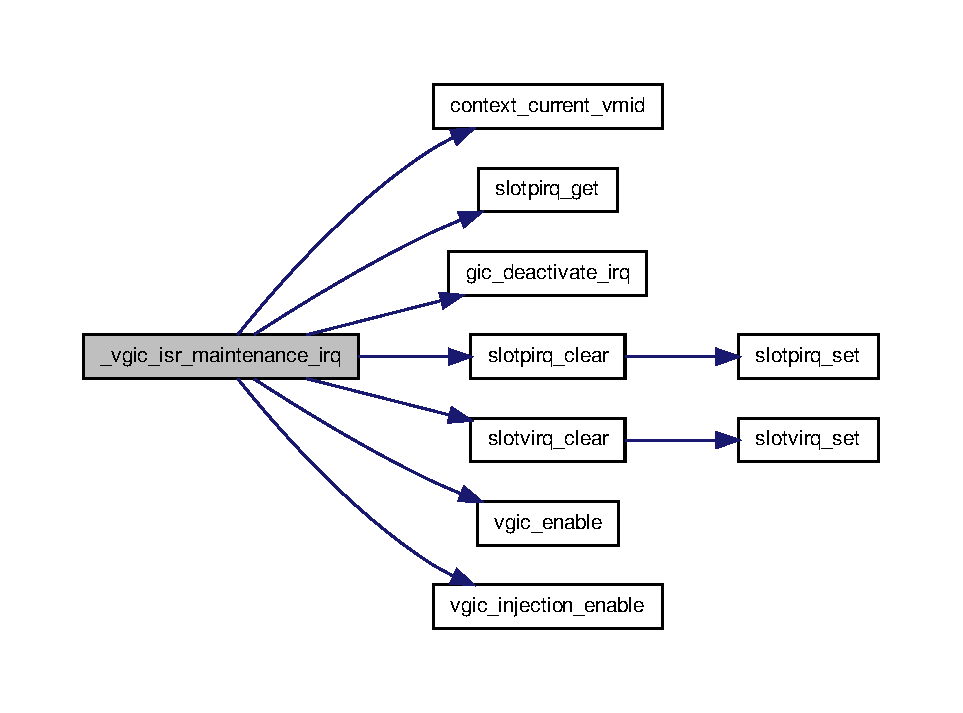
\includegraphics[width=350pt]{vgic_8c_a8d083941ad4202604d2ec7161c8f6409_cgraph}
\end{center}
\end{figure}


\hypertarget{vgic_8c_a66eca59dda59d2529191ca0c23094fc8}{\index{vgic.\-c@{vgic.\-c}!\-\_\-vgic\-\_\-valid\-\_\-lr\-\_\-mask@{\-\_\-vgic\-\_\-valid\-\_\-lr\-\_\-mask}}
\index{\-\_\-vgic\-\_\-valid\-\_\-lr\-\_\-mask@{\-\_\-vgic\-\_\-valid\-\_\-lr\-\_\-mask}!vgic.c@{vgic.\-c}}
\subsubsection[{\-\_\-vgic\-\_\-valid\-\_\-lr\-\_\-mask}]{\setlength{\rightskip}{0pt plus 5cm}static {\bf uint64\-\_\-t} {\bf \-\_\-vgic\-\_\-valid\-\_\-lr\-\_\-mask} (
\begin{DoxyParamCaption}
\item[{{\bf uint32\-\_\-t}}]{num\-\_\-lr}
\end{DoxyParamCaption}
)\hspace{0.3cm}{\ttfamily  \mbox{[}static\mbox{]}}}}\label{vgic_8c_a66eca59dda59d2529191ca0c23094fc8}


\-Definition at line 425 of file vgic.\-c.


\begin{DoxyCode}
{
    uint64_t mask_valid_lr = 0xFFFFFFFFFFFFFFFFULL;
    if ( num_lr < VGIC_MAX_LISTREGISTERS ) {
        mask_valid_lr >>= num_lr;
        mask_valid_lr <<= num_lr;
        mask_valid_lr = ~mask_valid_lr;
    }

    return mask_valid_lr;
}
\end{DoxyCode}
\hypertarget{vgic_8c_a4cf554520738a7934bc4e6917853330c}{\index{vgic.\-c@{vgic.\-c}!vgic\-\_\-enable@{vgic\-\_\-enable}}
\index{vgic\-\_\-enable@{vgic\-\_\-enable}!vgic.c@{vgic.\-c}}
\subsubsection[{vgic\-\_\-enable}]{\setlength{\rightskip}{0pt plus 5cm}{\bf hvmm\-\_\-status\-\_\-t} {\bf vgic\-\_\-enable} (
\begin{DoxyParamCaption}
\item[{{\bf uint8\-\_\-t}}]{enable}
\end{DoxyParamCaption}
)}}\label{vgic_8c_a4cf554520738a7934bc4e6917853330c}


\-Definition at line 277 of file vgic.\-c.


\begin{DoxyCode}
{
    hvmm_status_t result = HVMM_STATUS_BAD_ACCESS;

    if ( VGIC_READY() ) {

        if ( enable ) {
            uint32_t hcr = _vgic.base[GICH_HCR];

            hcr |= GICH_HCR_EN | GICH_HCR_NPIE;

            _vgic.base[GICH_HCR] = hcr;
        } else {
            _vgic.base[GICH_HCR] &= ~(GICH_HCR_EN | GICH_HCR_NPIE);
        }

        result = HVMM_STATUS_SUCCESS;
    } 
    return result;
}
\end{DoxyCode}
\hypertarget{vgic_8c_aab31fc8d2c44ebb938b78cfb1f7c975f}{\index{vgic.\-c@{vgic.\-c}!vgic\-\_\-find\-\_\-free\-\_\-slot@{vgic\-\_\-find\-\_\-free\-\_\-slot}}
\index{vgic\-\_\-find\-\_\-free\-\_\-slot@{vgic\-\_\-find\-\_\-free\-\_\-slot}!vgic.c@{vgic.\-c}}
\subsubsection[{vgic\-\_\-find\-\_\-free\-\_\-slot}]{\setlength{\rightskip}{0pt plus 5cm}static {\bf uint32\-\_\-t} {\bf vgic\-\_\-find\-\_\-free\-\_\-slot} (
\begin{DoxyParamCaption}
\item[{void}]{}
\end{DoxyParamCaption}
)\hspace{0.3cm}{\ttfamily  \mbox{[}static\mbox{]}}}}\label{vgic_8c_aab31fc8d2c44ebb938b78cfb1f7c975f}


\-Definition at line 82 of file vgic.\-c.


\begin{DoxyCode}
{
    uint32_t slot;
    uint32_t shift = 0;

    slot = _vgic.base[GICH_ELSR0];
    if ( slot == 0 && _vgic.num_lr > 32 ) {
        /* first 32 slots are occupied, try the later */
        slot = _vgic.base[GICH_ELSR1];
        shift = 32;
    }


    if ( slot ) {
        slot &= -(slot);
        slot = (31 - asm_clz(slot));
        slot += shift;
    } else {
        /* 64 slots are fully occupied */
        slot = VGIC_SLOT_NOTFOUND;
    }
    return slot;
}
\end{DoxyCode}
\hypertarget{vgic_8c_acb00c28d2618d3581a7d26f8e265ccb8}{\index{vgic.\-c@{vgic.\-c}!vgic\-\_\-flush\-\_\-virqs@{vgic\-\_\-flush\-\_\-virqs}}
\index{vgic\-\_\-flush\-\_\-virqs@{vgic\-\_\-flush\-\_\-virqs}!vgic.c@{vgic.\-c}}
\subsubsection[{vgic\-\_\-flush\-\_\-virqs}]{\setlength{\rightskip}{0pt plus 5cm}{\bf hvmm\-\_\-status\-\_\-t} {\bf vgic\-\_\-flush\-\_\-virqs} (
\begin{DoxyParamCaption}
\item[{{\bf vmid\-\_\-t}}]{vmid}
\end{DoxyParamCaption}
)}}\label{vgic_8c_acb00c28d2618d3581a7d26f8e265ccb8}


\-Definition at line 530 of file vgic.\-c.


\begin{DoxyCode}
{
    hvmm_status_t result = HVMM_STATUS_IGNORED;
    if ( _cb_virq_flush != 0 ) {
        _cb_virq_flush(vmid);
        result = HVMM_STATUS_SUCCESS;
    }

    return result;
}
\end{DoxyCode}
\hypertarget{vgic_8c_a2e0db8f93d8d6a61d737de34aeeed516}{\index{vgic.\-c@{vgic.\-c}!vgic\-\_\-init@{vgic\-\_\-init}}
\index{vgic\-\_\-init@{vgic\-\_\-init}!vgic.c@{vgic.\-c}}
\subsubsection[{vgic\-\_\-init}]{\setlength{\rightskip}{0pt plus 5cm}{\bf hvmm\-\_\-status\-\_\-t} {\bf vgic\-\_\-init} (
\begin{DoxyParamCaption}
\item[{void}]{}
\end{DoxyParamCaption}
)}}\label{vgic_8c_a2e0db8f93d8d6a61d737de34aeeed516}


\-Definition at line 451 of file vgic.\-c.


\begin{DoxyCode}
{
    hvmm_status_t result = HVMM_STATUS_UNKNOWN_ERROR;

    HVMM_TRACE_ENTER();

    _vgic.base = gic_vgic_baseaddr();
    _vgic.num_lr = (_vgic.base[GICH_VTR] & GICH_VTR_LISTREGS_MASK) + 1;
    _vgic.valid_lr_mask = _vgic_valid_lr_mask( _vgic.num_lr );
    _vgic.initialized = VGIC_SIGNATURE_INITIALIZED;

    vgic_maintenance_irq_enable(1);

    slotpirq_init();

    result = HVMM_STATUS_SUCCESS;

    _vgic_dump_status();
    _vgic_dump_regs();

    HVMM_TRACE_EXIT();
    return result;
}
\end{DoxyCode}


\-Here is the call graph for this function\-:
\nopagebreak
\begin{figure}[H]
\begin{center}
\leavevmode
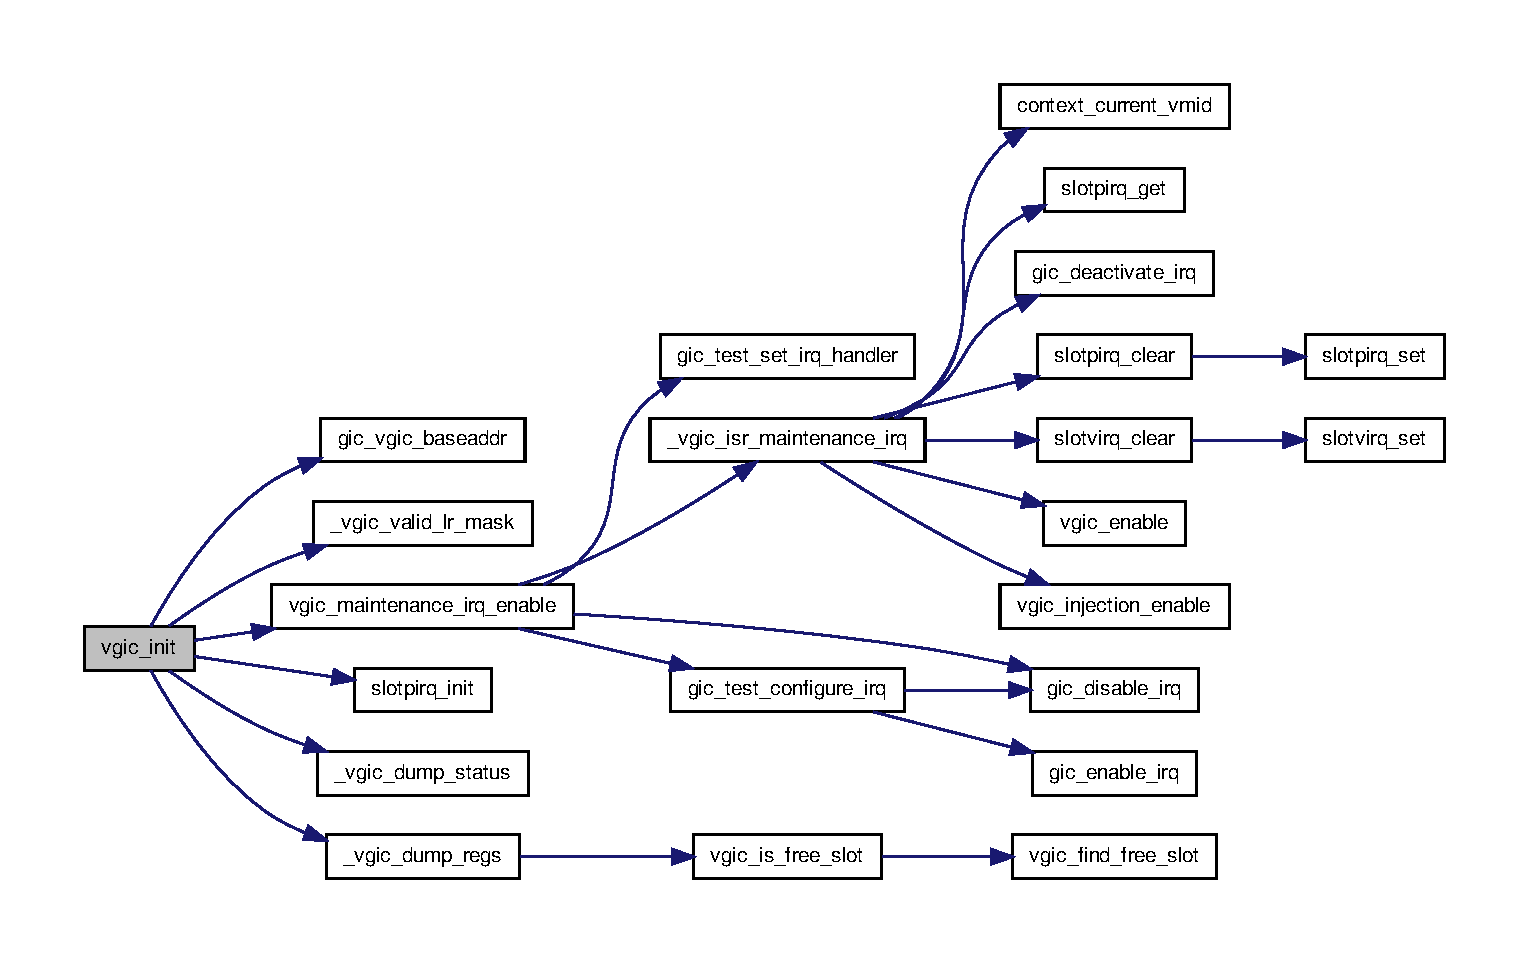
\includegraphics[width=350pt]{vgic_8c_a2e0db8f93d8d6a61d737de34aeeed516_cgraph}
\end{center}
\end{figure}


\hypertarget{vgic_8c_ac901a925af53a53bf1840d9be9acd2e0}{\index{vgic.\-c@{vgic.\-c}!vgic\-\_\-init\-\_\-status@{vgic\-\_\-init\-\_\-status}}
\index{vgic\-\_\-init\-\_\-status@{vgic\-\_\-init\-\_\-status}!vgic.c@{vgic.\-c}}
\subsubsection[{vgic\-\_\-init\-\_\-status}]{\setlength{\rightskip}{0pt plus 5cm}{\bf hvmm\-\_\-status\-\_\-t} {\bf vgic\-\_\-init\-\_\-status} (
\begin{DoxyParamCaption}
\item[{struct {\bf vgic\-\_\-status} $\ast$}]{status, }
\item[{{\bf vmid\-\_\-t}}]{vmid}
\end{DoxyParamCaption}
)}}\label{vgic_8c_ac901a925af53a53bf1840d9be9acd2e0}


\-Definition at line 475 of file vgic.\-c.


\begin{DoxyCode}
{
    hvmm_status_t result = HVMM_STATUS_SUCCESS;
    int i;

    status->hcr = 0;
    status->apr = 0;
    status->vmcr = 0;
    status->saved_once = 0;
    for( i = 0; i < _vgic.num_lr; i++) {
        status->lr[i] = 0;
    }

    return result;
}
\end{DoxyCode}
\hypertarget{vgic_8c_a6fb239504a0f9b77f78ca1f75318f78f}{\index{vgic.\-c@{vgic.\-c}!vgic\-\_\-inject\-\_\-virq@{vgic\-\_\-inject\-\_\-virq}}
\index{vgic\-\_\-inject\-\_\-virq@{vgic\-\_\-inject\-\_\-virq}!vgic.c@{vgic.\-c}}
\subsubsection[{vgic\-\_\-inject\-\_\-virq}]{\setlength{\rightskip}{0pt plus 5cm}{\bf uint32\-\_\-t} {\bf vgic\-\_\-inject\-\_\-virq} (
\begin{DoxyParamCaption}
\item[{{\bf uint32\-\_\-t}}]{virq, }
\item[{{\bf uint32\-\_\-t}}]{slot, }
\item[{{\bf virq\-\_\-state\-\_\-t}}]{state, }
\item[{{\bf uint32\-\_\-t}}]{priority, }
\item[{{\bf uint8\-\_\-t}}]{hw, }
\item[{{\bf uint32\-\_\-t}}]{physrc, }
\item[{{\bf uint8\-\_\-t}}]{maintenance}
\end{DoxyParamCaption}
)}}\label{vgic_8c_a6fb239504a0f9b77f78ca1f75318f78f}


\-Definition at line 332 of file vgic.\-c.


\begin{DoxyCode}
{
    uint32_t physicalid;
    uint32_t lr_desc;

    HVMM_TRACE_ENTER();

    physicalid = (hw ? physrc : (maintenance << 9) | (physrc & 0x7)) << 
      GICH_LR_PHYSICALID_SHIFT;
    physicalid &= GICH_LR_PHYSICALID_MASK;


    lr_desc = (GICH_LR_HW_MASK & (hw << GICH_LR_HW_SHIFT) ) |
        /* (GICH_LR_GRP1_MASK & (1 << GICH_LR_GRP1_SHIFT) )| */
        (GICH_LR_STATE_MASK & (state << GICH_LR_STATE_SHIFT) ) |
        (GICH_LR_PRIORITY_MASK & ( (priority >> 3)  << GICH_LR_PRIORITY_SHIFT) 
      ) |
        physicalid |
        (GICH_LR_VIRTUALID_MASK & virq );

    slot = vgic_is_free_slot( slot );

    HVMM_TRACE_HEX32("lr_desc:", lr_desc);
    HVMM_TRACE_HEX32("free slot:", slot);

    if ( slot != VGIC_SLOT_NOTFOUND ) {
        _vgic.base[GICH_LR + slot] = lr_desc;
        vgic_injection_enable(1);
        vgic_enable(1);
    }
    _vgic_dump_regs();

    HVMM_TRACE_EXIT();
    return slot;
}
\end{DoxyCode}


\-Here is the call graph for this function\-:
\nopagebreak
\begin{figure}[H]
\begin{center}
\leavevmode
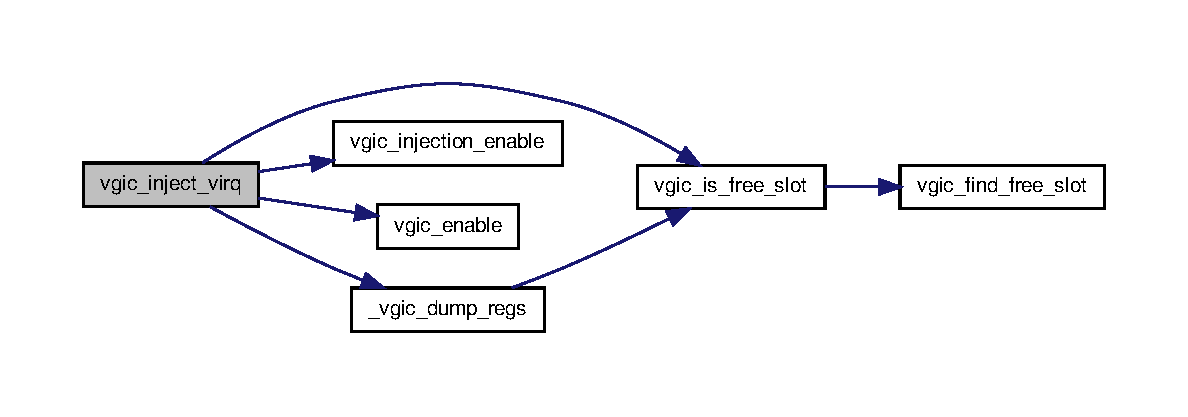
\includegraphics[width=350pt]{vgic_8c_a6fb239504a0f9b77f78ca1f75318f78f_cgraph}
\end{center}
\end{figure}


\hypertarget{vgic_8c_a93b048baf04857249e2ba3c24a82407f}{\index{vgic.\-c@{vgic.\-c}!vgic\-\_\-inject\-\_\-virq\-\_\-hw@{vgic\-\_\-inject\-\_\-virq\-\_\-hw}}
\index{vgic\-\_\-inject\-\_\-virq\-\_\-hw@{vgic\-\_\-inject\-\_\-virq\-\_\-hw}!vgic.c@{vgic.\-c}}
\subsubsection[{vgic\-\_\-inject\-\_\-virq\-\_\-hw}]{\setlength{\rightskip}{0pt plus 5cm}{\bf uint32\-\_\-t} {\bf vgic\-\_\-inject\-\_\-virq\-\_\-hw} (
\begin{DoxyParamCaption}
\item[{{\bf uint32\-\_\-t}}]{virq, }
\item[{{\bf virq\-\_\-state\-\_\-t}}]{state, }
\item[{{\bf uint32\-\_\-t}}]{priority, }
\item[{{\bf uint32\-\_\-t}}]{pirq}
\end{DoxyParamCaption}
)}}\label{vgic_8c_a93b048baf04857249e2ba3c24a82407f}


\-Definition at line 371 of file vgic.\-c.


\begin{DoxyCode}
{
    uint32_t slot = VGIC_SLOT_NOTFOUND;
    HVMM_TRACE_ENTER();

    slot = vgic_find_free_slot();
    HVMM_TRACE_HEX32("slot:", slot);
    if ( slot != VGIC_SLOT_NOTFOUND ) {
#ifdef VGIC_SIMULATE_HWVIRQ
        slot = vgic_inject_virq( virq, slot, state, priority, 0, 0, 1 );
#else
        slot = vgic_inject_virq( virq, slot, state, priority, 1, pirq, 0 );
#endif
    }

    HVMM_TRACE_EXIT();
    return slot;
}
\end{DoxyCode}


\-Here is the call graph for this function\-:
\nopagebreak
\begin{figure}[H]
\begin{center}
\leavevmode
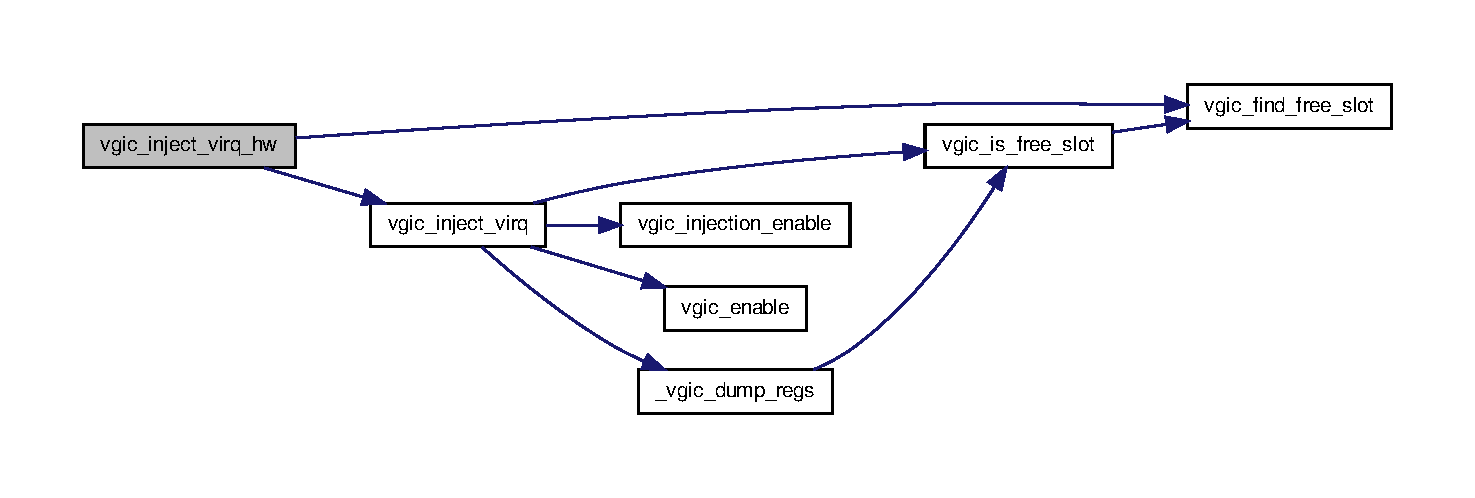
\includegraphics[width=350pt]{vgic_8c_a93b048baf04857249e2ba3c24a82407f_cgraph}
\end{center}
\end{figure}


\hypertarget{vgic_8c_a6fa5c258f61efb0140f0b85175d25ff5}{\index{vgic.\-c@{vgic.\-c}!vgic\-\_\-inject\-\_\-virq\-\_\-sw@{vgic\-\_\-inject\-\_\-virq\-\_\-sw}}
\index{vgic\-\_\-inject\-\_\-virq\-\_\-sw@{vgic\-\_\-inject\-\_\-virq\-\_\-sw}!vgic.c@{vgic.\-c}}
\subsubsection[{vgic\-\_\-inject\-\_\-virq\-\_\-sw}]{\setlength{\rightskip}{0pt plus 5cm}{\bf uint32\-\_\-t} {\bf vgic\-\_\-inject\-\_\-virq\-\_\-sw} (
\begin{DoxyParamCaption}
\item[{{\bf uint32\-\_\-t}}]{virq, }
\item[{{\bf virq\-\_\-state\-\_\-t}}]{state, }
\item[{{\bf uint32\-\_\-t}}]{priority, }
\item[{{\bf uint32\-\_\-t}}]{cpuid, }
\item[{{\bf uint8\-\_\-t}}]{maintenance}
\end{DoxyParamCaption}
)}}\label{vgic_8c_a6fa5c258f61efb0140f0b85175d25ff5}


\-Definition at line 390 of file vgic.\-c.


\begin{DoxyCode}
{
    uint32_t slot = VGIC_SLOT_NOTFOUND;
    HVMM_TRACE_ENTER();

    slot = vgic_find_free_slot();
    HVMM_TRACE_HEX32("slot:", slot);
    if ( slot != VGIC_SLOT_NOTFOUND ) {
        slot = vgic_inject_virq( virq, slot, state, priority, 0, cpuid, 
      maintenance );
    }

    HVMM_TRACE_EXIT();
    return slot;
}
\end{DoxyCode}


\-Here is the call graph for this function\-:
\nopagebreak
\begin{figure}[H]
\begin{center}
\leavevmode
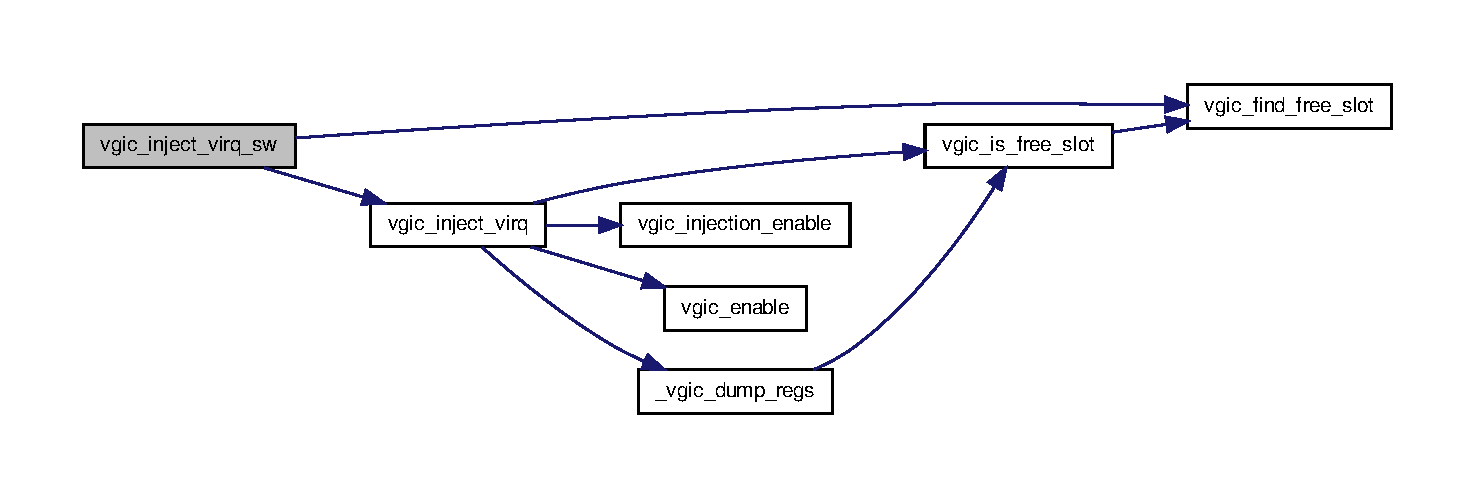
\includegraphics[width=350pt]{vgic_8c_a6fa5c258f61efb0140f0b85175d25ff5_cgraph}
\end{center}
\end{figure}


\hypertarget{vgic_8c_ae71b0763ed8149031b08ad13d8d687cb}{\index{vgic.\-c@{vgic.\-c}!vgic\-\_\-injection\-\_\-enable@{vgic\-\_\-injection\-\_\-enable}}
\index{vgic\-\_\-injection\-\_\-enable@{vgic\-\_\-injection\-\_\-enable}!vgic.c@{vgic.\-c}}
\subsubsection[{vgic\-\_\-injection\-\_\-enable}]{\setlength{\rightskip}{0pt plus 5cm}{\bf hvmm\-\_\-status\-\_\-t} {\bf vgic\-\_\-injection\-\_\-enable} (
\begin{DoxyParamCaption}
\item[{{\bf uint8\-\_\-t}}]{enable}
\end{DoxyParamCaption}
)}}\label{vgic_8c_ae71b0763ed8149031b08ad13d8d687cb}


\-Definition at line 298 of file vgic.\-c.


\begin{DoxyCode}
{
    uint32_t hcr;

    hcr = read_hcr();
    if ( enable ) {
        if ( (hcr & HCR_VI) == 0 ) {
            hcr |= HCR_VI;
            write_hcr(hcr);
        }
    } else {
        if ( hcr & HCR_VI ) {
            hcr &= ~(HCR_VI);
            write_hcr(hcr);
        }
    }

    hcr = read_hcr();
    printh( " updated hcr: %x\n", hcr);
    return HVMM_STATUS_SUCCESS;
}
\end{DoxyCode}
\hypertarget{vgic_8c_ac1d43326139a3717d69ce1f876cd221c}{\index{vgic.\-c@{vgic.\-c}!vgic\-\_\-is\-\_\-free\-\_\-slot@{vgic\-\_\-is\-\_\-free\-\_\-slot}}
\index{vgic\-\_\-is\-\_\-free\-\_\-slot@{vgic\-\_\-is\-\_\-free\-\_\-slot}!vgic.c@{vgic.\-c}}
\subsubsection[{vgic\-\_\-is\-\_\-free\-\_\-slot}]{\setlength{\rightskip}{0pt plus 5cm}static {\bf uint32\-\_\-t} {\bf vgic\-\_\-is\-\_\-free\-\_\-slot} (
\begin{DoxyParamCaption}
\item[{{\bf uint32\-\_\-t}}]{slot}
\end{DoxyParamCaption}
)\hspace{0.3cm}{\ttfamily  \mbox{[}static\mbox{]}}}}\label{vgic_8c_ac1d43326139a3717d69ce1f876cd221c}


\-Definition at line 114 of file vgic.\-c.


\begin{DoxyCode}
{
    uint32_t free_slot = VGIC_SLOT_NOTFOUND;
    
    if ( slot < 32 ) {
        if ( _vgic.base[GICH_ELSR0] & (1 << slot) )
            free_slot = slot;
    } else {
        if ( _vgic.base[GICH_ELSR1] & (1 << (slot - 32)) )
            free_slot = slot;
    }

    if ( free_slot != slot ) {
        free_slot = vgic_find_free_slot();
    }

    return free_slot;
}
\end{DoxyCode}


\-Here is the call graph for this function\-:
\nopagebreak
\begin{figure}[H]
\begin{center}
\leavevmode
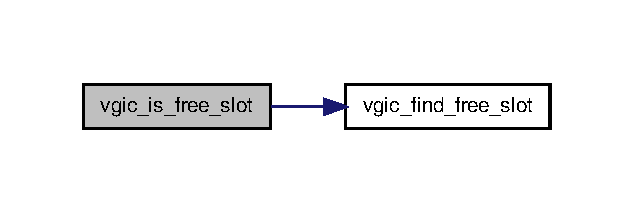
\includegraphics[width=304pt]{vgic_8c_ac1d43326139a3717d69ce1f876cd221c_cgraph}
\end{center}
\end{figure}


\hypertarget{vgic_8c_a896fa453c39e4d42fa37483b07c7d307}{\index{vgic.\-c@{vgic.\-c}!vgic\-\_\-maintenance\-\_\-irq\-\_\-enable@{vgic\-\_\-maintenance\-\_\-irq\-\_\-enable}}
\index{vgic\-\_\-maintenance\-\_\-irq\-\_\-enable@{vgic\-\_\-maintenance\-\_\-irq\-\_\-enable}!vgic.c@{vgic.\-c}}
\subsubsection[{vgic\-\_\-maintenance\-\_\-irq\-\_\-enable}]{\setlength{\rightskip}{0pt plus 5cm}{\bf hvmm\-\_\-status\-\_\-t} {\bf vgic\-\_\-maintenance\-\_\-irq\-\_\-enable} (
\begin{DoxyParamCaption}
\item[{{\bf uint8\-\_\-t}}]{enable}
\end{DoxyParamCaption}
)}}\label{vgic_8c_a896fa453c39e4d42fa37483b07c7d307}


\-Definition at line 406 of file vgic.\-c.


\begin{DoxyCode}
{
    uint32_t irq = VGIC_MAINTENANCE_INTERRUPT_IRQ;

    HVMM_TRACE_ENTER();
    if ( enable ) {
        gic_test_set_irq_handler( irq, &_vgic_isr_maintenance_irq, 0 );
        gic_test_configure_irq( irq,
                GIC_INT_POLARITY_LEVEL,
                gic_cpumask_current(),
                GIC_INT_PRIORITY_DEFAULT );
    } else {
        gic_test_set_irq_handler( irq, 0, 0 );
        gic_disable_irq( irq );
    }
    HVMM_TRACE_EXIT();
    return HVMM_STATUS_SUCCESS;
}
\end{DoxyCode}


\-Here is the call graph for this function\-:
\nopagebreak
\begin{figure}[H]
\begin{center}
\leavevmode
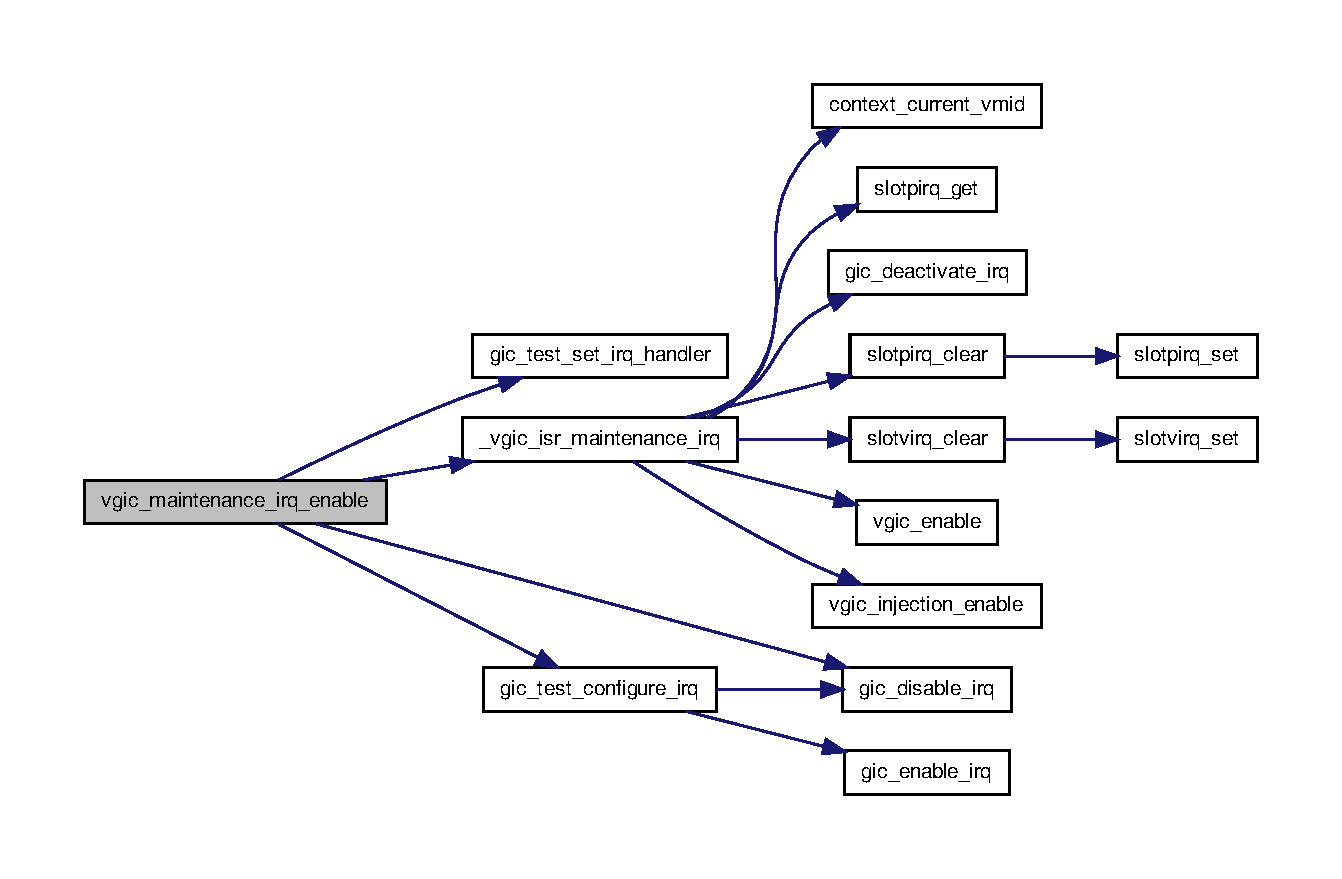
\includegraphics[width=350pt]{vgic_8c_a896fa453c39e4d42fa37483b07c7d307_cgraph}
\end{center}
\end{figure}


\hypertarget{vgic_8c_a70332a1790f88fbcb1a4c7014e6b6a02}{\index{vgic.\-c@{vgic.\-c}!vgic\-\_\-restore\-\_\-status@{vgic\-\_\-restore\-\_\-status}}
\index{vgic\-\_\-restore\-\_\-status@{vgic\-\_\-restore\-\_\-status}!vgic.c@{vgic.\-c}}
\subsubsection[{vgic\-\_\-restore\-\_\-status}]{\setlength{\rightskip}{0pt plus 5cm}{\bf hvmm\-\_\-status\-\_\-t} {\bf vgic\-\_\-restore\-\_\-status} (
\begin{DoxyParamCaption}
\item[{struct {\bf vgic\-\_\-status} $\ast$}]{status, }
\item[{{\bf vmid\-\_\-t}}]{vmid}
\end{DoxyParamCaption}
)}}\label{vgic_8c_a70332a1790f88fbcb1a4c7014e6b6a02}


\-Definition at line 509 of file vgic.\-c.


\begin{DoxyCode}
{
    hvmm_status_t result = HVMM_STATUS_BAD_ACCESS;
    int i;

    for( i = 0; i < _vgic.num_lr; i++) {
        _vgic.base[GICH_LR + i] = status->lr[i];
    }
    _vgic.base[GICH_APR] = status->apr;
    _vgic.base[GICH_VMCR] = status->vmcr;
    _vgic.base[GICH_HCR] = status->hcr;

    /* Inject queued virqs to the next guest */
    vgic_flush_virqs(vmid);

    _vgic_dump_regs();
    result = HVMM_STATUS_SUCCESS;

    return result;
}
\end{DoxyCode}


\-Here is the call graph for this function\-:
\nopagebreak
\begin{figure}[H]
\begin{center}
\leavevmode
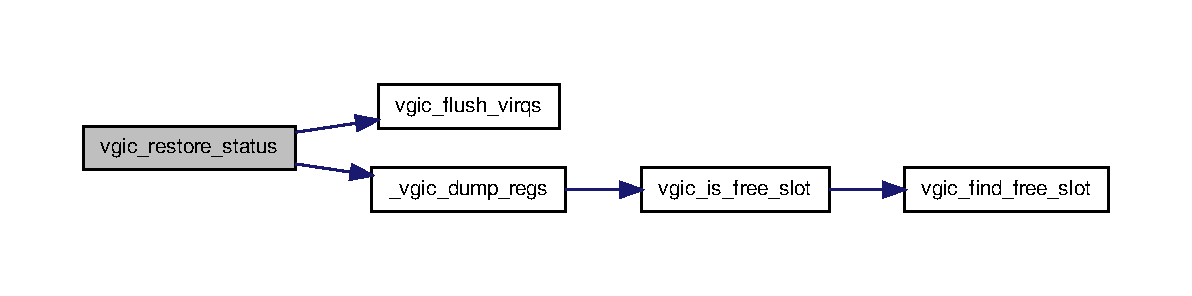
\includegraphics[width=350pt]{vgic_8c_a70332a1790f88fbcb1a4c7014e6b6a02_cgraph}
\end{center}
\end{figure}


\hypertarget{vgic_8c_aebad7b956b2c36d2bbe7acdbe333ae8a}{\index{vgic.\-c@{vgic.\-c}!vgic\-\_\-save\-\_\-status@{vgic\-\_\-save\-\_\-status}}
\index{vgic\-\_\-save\-\_\-status@{vgic\-\_\-save\-\_\-status}!vgic.c@{vgic.\-c}}
\subsubsection[{vgic\-\_\-save\-\_\-status}]{\setlength{\rightskip}{0pt plus 5cm}{\bf hvmm\-\_\-status\-\_\-t} {\bf vgic\-\_\-save\-\_\-status} (
\begin{DoxyParamCaption}
\item[{struct {\bf vgic\-\_\-status} $\ast$}]{status, }
\item[{{\bf vmid\-\_\-t}}]{vmid}
\end{DoxyParamCaption}
)}}\label{vgic_8c_aebad7b956b2c36d2bbe7acdbe333ae8a}


\-Definition at line 491 of file vgic.\-c.


\begin{DoxyCode}
{
    hvmm_status_t result = HVMM_STATUS_SUCCESS;
    int i;


    for( i = 0; i < _vgic.num_lr; i++ ) {
        status->lr[i] = _vgic.base[GICH_LR + i];
    }
    status->hcr = _vgic.base[GICH_HCR];
    status->apr = _vgic.base[GICH_APR];
    status->vmcr = _vgic.base[GICH_VMCR];
    status->saved_once = VGIC_SIGNATURE_INITIALIZED;

    vgic_enable(0);
    return result;
}
\end{DoxyCode}


\-Here is the call graph for this function\-:
\nopagebreak
\begin{figure}[H]
\begin{center}
\leavevmode
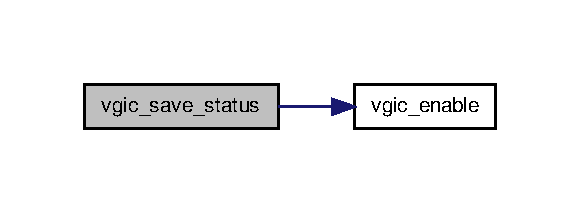
\includegraphics[width=278pt]{vgic_8c_aebad7b956b2c36d2bbe7acdbe333ae8a_cgraph}
\end{center}
\end{figure}


\hypertarget{vgic_8c_a2302c75a54486f179f199997b4a268b3}{\index{vgic.\-c@{vgic.\-c}!vgic\-\_\-setcallback\-\_\-virq\-\_\-flush@{vgic\-\_\-setcallback\-\_\-virq\-\_\-flush}}
\index{vgic\-\_\-setcallback\-\_\-virq\-\_\-flush@{vgic\-\_\-setcallback\-\_\-virq\-\_\-flush}!vgic.c@{vgic.\-c}}
\subsubsection[{vgic\-\_\-setcallback\-\_\-virq\-\_\-flush}]{\setlength{\rightskip}{0pt plus 5cm}{\bf hvmm\-\_\-status\-\_\-t} {\bf vgic\-\_\-setcallback\-\_\-virq\-\_\-flush} (
\begin{DoxyParamCaption}
\item[{void($\ast$)({\bf vmid\-\_\-t} vmid)}]{callback}
\end{DoxyParamCaption}
)}}\label{vgic_8c_a2302c75a54486f179f199997b4a268b3}


\-Definition at line 440 of file vgic.\-c.


\begin{DoxyCode}
{
    _cb_virq_flush = callback;
    if ( _cb_virq_flush == 0 ) {
        printh( "vgic: virq_flush() cleared\n" );
    } else {
        printh( "vgic: virq_flush() set to function at %x\n", (uint32_t) 
      _cb_virq_flush );
    }
    return HVMM_STATUS_SUCCESS;
}
\end{DoxyCode}


\subsection{\-Variable \-Documentation}
\hypertarget{vgic_8c_a91dbbb7f0fc3b51b2cc9482aaa444d39}{\index{vgic.\-c@{vgic.\-c}!\-\_\-cb\-\_\-virq\-\_\-flush@{\-\_\-cb\-\_\-virq\-\_\-flush}}
\index{\-\_\-cb\-\_\-virq\-\_\-flush@{\-\_\-cb\-\_\-virq\-\_\-flush}!vgic.c@{vgic.\-c}}
\subsubsection[{\-\_\-cb\-\_\-virq\-\_\-flush}]{\setlength{\rightskip}{0pt plus 5cm}void($\ast$ {\bf \-\_\-cb\-\_\-virq\-\_\-flush})({\bf vmid\-\_\-t} vmid)=0\hspace{0.3cm}{\ttfamily  \mbox{[}static\mbox{]}}}}\label{vgic_8c_a91dbbb7f0fc3b51b2cc9482aaa444d39}


\-Definition at line 80 of file vgic.\-c.

\hypertarget{vgic_8c_a5191716b54330506bb98f687550f2812}{\index{vgic.\-c@{vgic.\-c}!\-\_\-vgic@{\-\_\-vgic}}
\index{\-\_\-vgic@{\-\_\-vgic}!vgic.c@{vgic.\-c}}
\subsubsection[{\-\_\-vgic}]{\setlength{\rightskip}{0pt plus 5cm}struct {\bf vgic} {\bf \-\_\-vgic}\hspace{0.3cm}{\ttfamily  \mbox{[}static\mbox{]}}}}\label{vgic_8c_a5191716b54330506bb98f687550f2812}


\-Definition at line 79 of file vgic.\-c.


\hypertarget{hyp__config_8h}{\section{hyp\-\_\-config.\-h \-File \-Reference}
\label{hyp__config_8h}\index{hyp\-\_\-config.\-h@{hyp\-\_\-config.\-h}}
}
\subsection*{\-Defines}
\begin{DoxyCompactItemize}
\item 
\#define \hyperlink{hyp__config_8h_a7fcfcbc766cea81a21e2d8aba3b54843}{\-N\-U\-M\-\_\-\-G\-U\-E\-S\-T\-S\-\_\-\-S\-T\-A\-T\-I\-C}~2
\end{DoxyCompactItemize}


\subsection{\-Define \-Documentation}
\hypertarget{hyp__config_8h_a7fcfcbc766cea81a21e2d8aba3b54843}{\index{hyp\-\_\-config.\-h@{hyp\-\_\-config.\-h}!\-N\-U\-M\-\_\-\-G\-U\-E\-S\-T\-S\-\_\-\-S\-T\-A\-T\-I\-C@{\-N\-U\-M\-\_\-\-G\-U\-E\-S\-T\-S\-\_\-\-S\-T\-A\-T\-I\-C}}
\index{\-N\-U\-M\-\_\-\-G\-U\-E\-S\-T\-S\-\_\-\-S\-T\-A\-T\-I\-C@{\-N\-U\-M\-\_\-\-G\-U\-E\-S\-T\-S\-\_\-\-S\-T\-A\-T\-I\-C}!hyp_config.h@{hyp\-\_\-config.\-h}}
\subsubsection[{\-N\-U\-M\-\_\-\-G\-U\-E\-S\-T\-S\-\_\-\-S\-T\-A\-T\-I\-C}]{\setlength{\rightskip}{0pt plus 5cm}\#define {\bf \-N\-U\-M\-\_\-\-G\-U\-E\-S\-T\-S\-\_\-\-S\-T\-A\-T\-I\-C}~2}}\label{hyp__config_8h_a7fcfcbc766cea81a21e2d8aba3b54843}


\-Definition at line 4 of file hyp\-\_\-config.\-h.


\hypertarget{a15__cp15__sysregs_8h}{\section{include/a15\-\_\-cp15\-\_\-sysregs.h \-File \-Reference}
\label{a15__cp15__sysregs_8h}\index{include/a15\-\_\-cp15\-\_\-sysregs.\-h@{include/a15\-\_\-cp15\-\_\-sysregs.\-h}}
}
{\ttfamily \#include \char`\"{}arch\-\_\-types.\-h\char`\"{}}\*
\-Include dependency graph for a15\-\_\-cp15\-\_\-sysregs.\-h\-:
\nopagebreak
\begin{figure}[H]
\begin{center}
\leavevmode
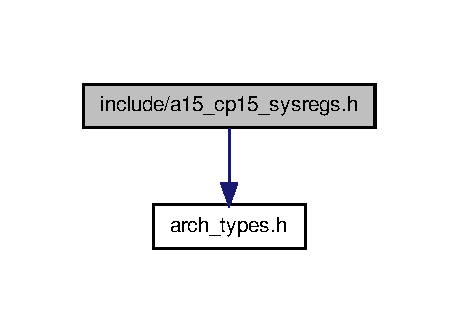
\includegraphics[width=220pt]{a15__cp15__sysregs_8h__incl}
\end{center}
\end{figure}
\-This graph shows which files directly or indirectly include this file\-:
\nopagebreak
\begin{figure}[H]
\begin{center}
\leavevmode
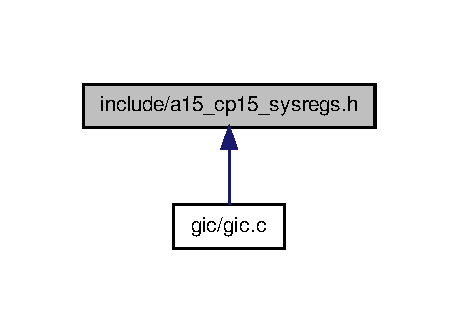
\includegraphics[width=220pt]{a15__cp15__sysregs_8h__dep__incl}
\end{center}
\end{figure}
\subsection*{\-Defines}
\begin{DoxyCompactItemize}
\item 
\#define \hyperlink{a15__cp15__sysregs_8h_a3f300d071bd93f39214079dbe23891bc}{read\-\_\-cbar}()
\end{DoxyCompactItemize}


\subsection{\-Define \-Documentation}
\hypertarget{a15__cp15__sysregs_8h_a3f300d071bd93f39214079dbe23891bc}{\index{a15\-\_\-cp15\-\_\-sysregs.\-h@{a15\-\_\-cp15\-\_\-sysregs.\-h}!read\-\_\-cbar@{read\-\_\-cbar}}
\index{read\-\_\-cbar@{read\-\_\-cbar}!a15_cp15_sysregs.h@{a15\-\_\-cp15\-\_\-sysregs.\-h}}
\subsubsection[{read\-\_\-cbar}]{\setlength{\rightskip}{0pt plus 5cm}\#define {\bf read\-\_\-cbar}(
\begin{DoxyParamCaption}
{}
\end{DoxyParamCaption}
)}}\label{a15__cp15__sysregs_8h_a3f300d071bd93f39214079dbe23891bc}
{\bfseries \-Value\-:}
\begin{DoxyCode}
({ uint32_t rval; asm volatile(\
                                " mrc     p15, 4, %0, c15, c0, 0\n\t" \
                                : "=r" (rval) : : "memory", "cc"); rval;})
\end{DoxyCode}


\-Definition at line 26 of file a15\-\_\-cp15\-\_\-sysregs.\-h.


\hypertarget{arch__types_8h}{\section{include/arch\-\_\-types.h \-File \-Reference}
\label{arch__types_8h}\index{include/arch\-\_\-types.\-h@{include/arch\-\_\-types.\-h}}
}
\-This graph shows which files directly or indirectly include this file\-:
\nopagebreak
\begin{figure}[H]
\begin{center}
\leavevmode
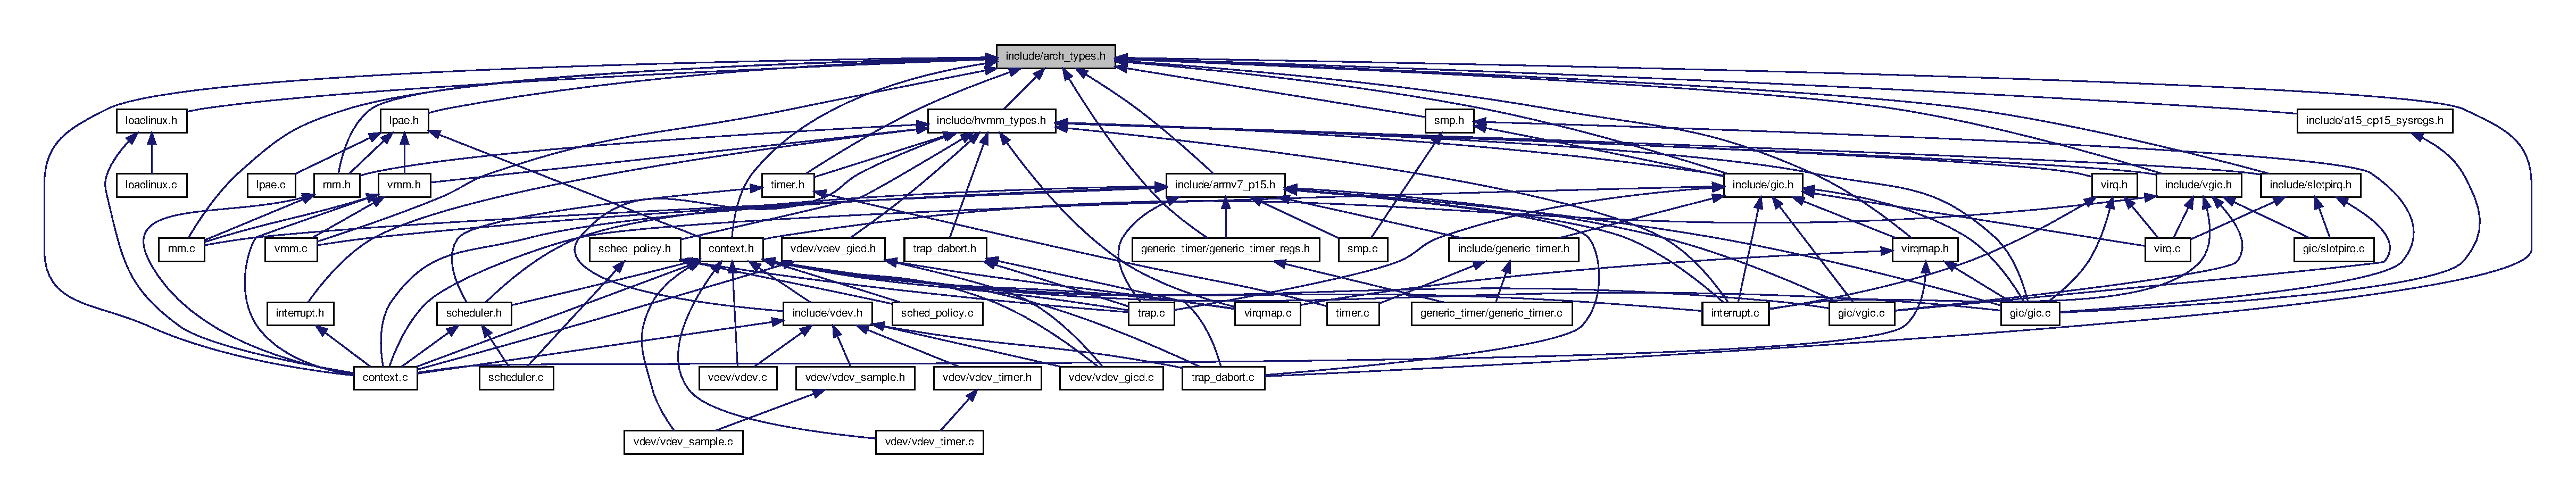
\includegraphics[width=350pt]{arch__types_8h__dep__incl}
\end{center}
\end{figure}
\subsection*{\-Typedefs}
\begin{DoxyCompactItemize}
\item 
typedef int \hyperlink{arch__types_8h_a32f2e37ee053cf2ce8ca28d1f74630e5}{int32\-\_\-t}
\item 
typedef unsigned int \hyperlink{arch__types_8h_a435d1572bf3f880d55459d9805097f62}{uint32\-\_\-t}
\item 
typedef unsigned short \hyperlink{arch__types_8h_a273cf69d639a59973b6019625df33e30}{uint16\-\_\-t}
\item 
typedef unsigned long long \hyperlink{arch__types_8h_aaa5d1cd013383c889537491c3cfd9aad}{uint64\-\_\-t}
\item 
typedef unsigned char \hyperlink{arch__types_8h_aba7bc1797add20fe3efdf37ced1182c5}{uint8\-\_\-t}
\end{DoxyCompactItemize}


\subsection{\-Typedef \-Documentation}
\hypertarget{arch__types_8h_a32f2e37ee053cf2ce8ca28d1f74630e5}{\index{arch\-\_\-types.\-h@{arch\-\_\-types.\-h}!int32\-\_\-t@{int32\-\_\-t}}
\index{int32\-\_\-t@{int32\-\_\-t}!arch_types.h@{arch\-\_\-types.\-h}}
\subsubsection[{int32\-\_\-t}]{\setlength{\rightskip}{0pt plus 5cm}typedef int {\bf int32\-\_\-t}}}\label{arch__types_8h_a32f2e37ee053cf2ce8ca28d1f74630e5}


\-Definition at line 4 of file arch\-\_\-types.\-h.

\hypertarget{arch__types_8h_a273cf69d639a59973b6019625df33e30}{\index{arch\-\_\-types.\-h@{arch\-\_\-types.\-h}!uint16\-\_\-t@{uint16\-\_\-t}}
\index{uint16\-\_\-t@{uint16\-\_\-t}!arch_types.h@{arch\-\_\-types.\-h}}
\subsubsection[{uint16\-\_\-t}]{\setlength{\rightskip}{0pt plus 5cm}typedef unsigned short {\bf uint16\-\_\-t}}}\label{arch__types_8h_a273cf69d639a59973b6019625df33e30}


\-Definition at line 6 of file arch\-\_\-types.\-h.

\hypertarget{arch__types_8h_a435d1572bf3f880d55459d9805097f62}{\index{arch\-\_\-types.\-h@{arch\-\_\-types.\-h}!uint32\-\_\-t@{uint32\-\_\-t}}
\index{uint32\-\_\-t@{uint32\-\_\-t}!arch_types.h@{arch\-\_\-types.\-h}}
\subsubsection[{uint32\-\_\-t}]{\setlength{\rightskip}{0pt plus 5cm}typedef unsigned int {\bf uint32\-\_\-t}}}\label{arch__types_8h_a435d1572bf3f880d55459d9805097f62}


\-Definition at line 5 of file arch\-\_\-types.\-h.

\hypertarget{arch__types_8h_aaa5d1cd013383c889537491c3cfd9aad}{\index{arch\-\_\-types.\-h@{arch\-\_\-types.\-h}!uint64\-\_\-t@{uint64\-\_\-t}}
\index{uint64\-\_\-t@{uint64\-\_\-t}!arch_types.h@{arch\-\_\-types.\-h}}
\subsubsection[{uint64\-\_\-t}]{\setlength{\rightskip}{0pt plus 5cm}typedef unsigned long long {\bf uint64\-\_\-t}}}\label{arch__types_8h_aaa5d1cd013383c889537491c3cfd9aad}


\-Definition at line 7 of file arch\-\_\-types.\-h.

\hypertarget{arch__types_8h_aba7bc1797add20fe3efdf37ced1182c5}{\index{arch\-\_\-types.\-h@{arch\-\_\-types.\-h}!uint8\-\_\-t@{uint8\-\_\-t}}
\index{uint8\-\_\-t@{uint8\-\_\-t}!arch_types.h@{arch\-\_\-types.\-h}}
\subsubsection[{uint8\-\_\-t}]{\setlength{\rightskip}{0pt plus 5cm}typedef unsigned char {\bf uint8\-\_\-t}}}\label{arch__types_8h_aba7bc1797add20fe3efdf37ced1182c5}


\-Definition at line 8 of file arch\-\_\-types.\-h.


\hypertarget{armv7__p15_8h}{\section{include/armv7\-\_\-p15.h \-File \-Reference}
\label{armv7__p15_8h}\index{include/armv7\-\_\-p15.\-h@{include/armv7\-\_\-p15.\-h}}
}
{\ttfamily \#include \char`\"{}arch\-\_\-types.\-h\char`\"{}}\*
\-Include dependency graph for armv7\-\_\-p15.\-h\-:
\nopagebreak
\begin{figure}[H]
\begin{center}
\leavevmode
\includegraphics[width=186pt]{armv7__p15_8h__incl}
\end{center}
\end{figure}
\-This graph shows which files directly or indirectly include this file\-:
\nopagebreak
\begin{figure}[H]
\begin{center}
\leavevmode
\includegraphics[width=350pt]{armv7__p15_8h__dep__incl}
\end{center}
\end{figure}
\subsection*{\-Defines}
\begin{DoxyCompactItemize}
\item 
\#define \hyperlink{armv7__p15_8h_ace8367d12c7d122830035d2c9708f3ed}{read\-\_\-cpsr}()
\item 
\#define \hyperlink{armv7__p15_8h_a0c86d33c8981873c7ecad9fc9f8aceaf}{read\-\_\-vbar}()
\item 
\#define \hyperlink{armv7__p15_8h_a4e31e0e9a65d81a76a699f5acfac2679}{write\-\_\-vbar}(val)
\item 
\#define \hyperlink{armv7__p15_8h_a2aa0eef043f2325faf7e08f0c22aa9ed}{\-H\-C\-R\-\_\-\-F\-M\-O}~0x8
\item 
\#define \hyperlink{armv7__p15_8h_a8d290f53f0e3d6ec4eb4ea9326dfb238}{\-H\-C\-R\-\_\-\-I\-M\-O}~0x10
\item 
\#define \hyperlink{armv7__p15_8h_a7f64ef8930b21947c90bf648774c6d7a}{\-H\-C\-R\-\_\-\-V\-I}~(0x1 $<$$<$ 7)
\item 
\#define \hyperlink{armv7__p15_8h_a4ccd5f7d934e0e5d70f2efa015f24826}{read\-\_\-ttbr0}()
\item 
\#define \hyperlink{armv7__p15_8h_aef4ad3f99a91f73dd5ea72a9f08c684d}{write\-\_\-ttbr0}(val)
\item 
\#define \hyperlink{armv7__p15_8h_a0f00f0b592454cc49a97e37135bae154}{read\-\_\-ttbr1}()
\item 
\#define \hyperlink{armv7__p15_8h_a3113363b11bd015751a6fac65457c3ef}{write\-\_\-ttbr1}(val)
\item 
\#define \hyperlink{armv7__p15_8h_ab108290b06009cda35888c4e3cf0e186}{read\-\_\-ttbcr}()
\item 
\#define \hyperlink{armv7__p15_8h_a7a2b03678768ed709e85cf17ff7177e0}{write\-\_\-ttbcr}(val)
\item 
\#define \hyperlink{armv7__p15_8h_a9be943306a7c8c92e242d7b0c528c104}{read\-\_\-mair0}()
\item 
\#define \hyperlink{armv7__p15_8h_a4c688b4baf4bb99717ab883ec98731e3}{write\-\_\-mair0}(val)
\item 
\#define \hyperlink{armv7__p15_8h_a4202580631120ea819013536d1764714}{read\-\_\-mair1}()
\item 
\#define \hyperlink{armv7__p15_8h_a95ccc5e9e75f16d92e86e8c5e8795021}{write\-\_\-mair1}(val)
\item 
\#define \hyperlink{armv7__p15_8h_ad0f95cce118c43e27e56c573d2474589}{read\-\_\-hmair0}()
\item 
\#define \hyperlink{armv7__p15_8h_aceed5bc8f6ff935f285f0151d02984f4}{write\-\_\-hmair0}(val)
\item 
\#define \hyperlink{armv7__p15_8h_a9c20c8c67832c7220daa6decf3716d3a}{read\-\_\-hmair1}()
\item 
\#define \hyperlink{armv7__p15_8h_a28ff414c50b9d208a74c509495c03798}{write\-\_\-hmair1}(val)
\item 
\#define \hyperlink{armv7__p15_8h_aa41bd8bfa37a46e776d56ce2d7e4d083}{read\-\_\-hsr}()
\item 
\#define \hyperlink{armv7__p15_8h_a3a6bae959f288dba466eaf69ddb942af}{read\-\_\-htcr}()
\item 
\#define \hyperlink{armv7__p15_8h_ac82f4f6d095d646b4c5dfe8ada9fb08b}{write\-\_\-htcr}(val)
\item 
\#define \hyperlink{armv7__p15_8h_a13913f74bb5cce3c362082e705da87db}{read\-\_\-hsctlr}()
\item 
\#define \hyperlink{armv7__p15_8h_a94fd8feb077baacec23b5626e75052d2}{write\-\_\-hsctlr}(val)
\item 
\#define \hyperlink{armv7__p15_8h_ad17d4af13acc1a347d253dcc32c25881}{read\-\_\-sctlr}()
\item 
\#define \hyperlink{armv7__p15_8h_ae7e49f9effb0c96c1045ceddae9cadf5}{write\-\_\-sctlr}(val)
\item 
\#define \hyperlink{armv7__p15_8h_a814b3bae099b30c902bcd707bb4293a1}{read\-\_\-httbr}()
\item 
\#define \hyperlink{armv7__p15_8h_aadd0a0d0ee622916cac09b282b6b30ac}{write\-\_\-httbr}(val)
\item 
\#define \hyperlink{armv7__p15_8h_a228f19aa25c4d23dee8a0be5b41691d9}{read\-\_\-vtcr}()
\item 
\#define \hyperlink{armv7__p15_8h_a3982aeb15e1c94c960d0d0fdec2a4486}{write\-\_\-vtcr}(val)
\item 
\#define \hyperlink{armv7__p15_8h_a4e4681628f215ab9436d9376e67ec931}{read\-\_\-vttbr}()
\item 
\#define \hyperlink{armv7__p15_8h_af3a68551ffa6743c517c720afea598a6}{write\-\_\-vttbr}(val)
\item 
\#define \hyperlink{armv7__p15_8h_a3b7662f2d5a21a8a49f06da2a29483ec}{read\-\_\-hcr}()
\item 
\#define \hyperlink{armv7__p15_8h_ab2fd766fe3ad6974730d990af8af1aad}{write\-\_\-hcr}(val)
\item 
\#define \hyperlink{armv7__p15_8h_a9a17b04c7e79b8a7c7a088d6e9f9c2f8}{read\-\_\-midr}()
\item 
\#define \hyperlink{armv7__p15_8h_ae7a3ffe94082726164ef99da5c940198}{read\-\_\-mpidr}()
\item 
\#define \hyperlink{armv7__p15_8h_a22dc1998cdb4bde4c7fb58dbdf4c61b7}{read\-\_\-cntfrq}()
\item 
\#define \hyperlink{armv7__p15_8h_a36916f645a1d1af13328e2760a6e758b}{write\-\_\-cntfrq}(val)
\item 
\#define \hyperlink{armv7__p15_8h_afb75f009f97a77ef70a8af5af59e9b51}{read\-\_\-cnthctl}()
\item 
\#define \hyperlink{armv7__p15_8h_a45db513be8ffc7a00ccaf1ff2faab49d}{write\-\_\-cnthctl}(val)
\item 
\#define \hyperlink{armv7__p15_8h_aa6a9055f0f8ef1f1c31a64d934f2fcc1}{read\-\_\-cnthp\-\_\-ctl}()
\item 
\#define \hyperlink{armv7__p15_8h_a419fbc198bfa7aed2fdc2b3bf8a80c75}{write\-\_\-cnthp\-\_\-ctl}(val)
\item 
\#define \hyperlink{armv7__p15_8h_a25fd6098094a06ac618bdf5a03411747}{read\-\_\-cnthp\-\_\-cval}()
\item 
\#define \hyperlink{armv7__p15_8h_a858012a8a45700f96e58971a6fd318e6}{write\-\_\-cnthp\-\_\-cval}(val)
\item 
\#define \hyperlink{armv7__p15_8h_af447e860889e18fa7aeb645ce7f6d328}{read\-\_\-cnthp\-\_\-tval}()
\item 
\#define \hyperlink{armv7__p15_8h_a317588a5fac9e97233e604c8e43716f4}{write\-\_\-cnthp\-\_\-tval}(val)
\item 
\#define \hyperlink{armv7__p15_8h_a0fa1be710f0b34cded7d854664ca0892}{read\-\_\-cntkctl}()
\item 
\#define \hyperlink{armv7__p15_8h_aab3ac35bac93fb1d81d77043bf9feba3}{write\-\_\-cntkctl}(val)
\item 
\#define \hyperlink{armv7__p15_8h_a62454f186d32571ba5b0ef9501d1a780}{read\-\_\-cntp\-\_\-ctl}()
\item 
\#define \hyperlink{armv7__p15_8h_ab6947eb7aa7224ff40daf1641196c4f7}{write\-\_\-cntp\-\_\-ctl}(val)
\item 
\#define \hyperlink{armv7__p15_8h_a6af8a4385ce10e17702b7f2db00aecd0}{read\-\_\-cntp\-\_\-cval}()
\item 
\#define \hyperlink{armv7__p15_8h_a59cd6778741b413df8b81a46a4e621f2}{write\-\_\-cntp\-\_\-cval}(val)
\item 
\#define \hyperlink{armv7__p15_8h_a2b8d99e8ddfcce1608f762994ea80e2e}{read\-\_\-cntp\-\_\-tval}()
\item 
\#define \hyperlink{armv7__p15_8h_a0940385a164613a8b2864940683b4fb2}{write\-\_\-cntp\-\_\-tval}(val)
\item 
\#define \hyperlink{armv7__p15_8h_a4939c99e7b83a6fbef2867ab52240464}{read\-\_\-cntpct}()
\item 
\#define \hyperlink{armv7__p15_8h_a1b415ea5f339065c53f4db29a7e21af2}{read\-\_\-cntv\-\_\-ctl}()
\item 
\#define \hyperlink{armv7__p15_8h_a8a9b7c864d5560d421e8a3c3bc8dca84}{write\-\_\-cntv\-\_\-ctl}(val)
\item 
\#define \hyperlink{armv7__p15_8h_a26c9aea7ac28377126ecc15ea29dd6bc}{read\-\_\-cntv\-\_\-cval}()
\item 
\#define \hyperlink{armv7__p15_8h_a2f39865e58552372917fb13d964cc4c3}{write\-\_\-cntv\-\_\-cval}(val)
\item 
\#define \hyperlink{armv7__p15_8h_a2fcd5fc1f26aefe55daa5ce989f88b46}{read\-\_\-cntv\-\_\-tval}()
\item 
\#define \hyperlink{armv7__p15_8h_a7c703e3a685054390f3220697504961c}{write\-\_\-cntv\-\_\-tval}(val)
\item 
\#define \hyperlink{armv7__p15_8h_a12e577d17891dc46fcc76e72f6bbd9f0}{read\-\_\-cntvct}()
\item 
\#define \hyperlink{armv7__p15_8h_afd7fe5fb860932b7a45f3bdad5973408}{read\-\_\-cntvoff}()
\item 
\#define \hyperlink{armv7__p15_8h_ab6c927f0e1c9f7293b06d710d6142fc2}{write\-\_\-cntvoff}(val)
\item 
\#define \hyperlink{armv7__p15_8h_a2c835cd674781985c210053d70b64e0d}{read\-\_\-hdfar}()
\item 
\#define \hyperlink{armv7__p15_8h_a91e91a685893da52c1f120e7f98a1280}{write\-\_\-hdfar}(val)
\item 
\#define \hyperlink{armv7__p15_8h_a491b0104eb0e24c25285c8e90e101cd1}{read\-\_\-hifar}()
\item 
\#define \hyperlink{armv7__p15_8h_a3aef95a08f0a64a8f8c485927edc3873}{write\-\_\-hifar}(val)
\item 
\#define \hyperlink{armv7__p15_8h_a8e2ca9957a561bdfab81184207fb9166}{read\-\_\-hpfar}()
\item 
\#define \hyperlink{armv7__p15_8h_a4068a00c498d7bf185423870909d0642}{write\-\_\-hpfar}(val)
\item 
\#define \hyperlink{armv7__p15_8h_a8983432e251fc0069019ae2e253e1765}{invalidate\-\_\-unified\-\_\-tlb}(val)
\end{DoxyCompactItemize}


\subsection{\-Define \-Documentation}
\hypertarget{armv7__p15_8h_a2aa0eef043f2325faf7e08f0c22aa9ed}{\index{armv7\-\_\-p15.\-h@{armv7\-\_\-p15.\-h}!\-H\-C\-R\-\_\-\-F\-M\-O@{\-H\-C\-R\-\_\-\-F\-M\-O}}
\index{\-H\-C\-R\-\_\-\-F\-M\-O@{\-H\-C\-R\-\_\-\-F\-M\-O}!armv7_p15.h@{armv7\-\_\-p15.\-h}}
\subsubsection[{\-H\-C\-R\-\_\-\-F\-M\-O}]{\setlength{\rightskip}{0pt plus 5cm}\#define {\bf \-H\-C\-R\-\_\-\-F\-M\-O}~0x8}}\label{armv7__p15_8h_a2aa0eef043f2325faf7e08f0c22aa9ed}


\-Definition at line 18 of file armv7\-\_\-p15.\-h.

\hypertarget{armv7__p15_8h_a8d290f53f0e3d6ec4eb4ea9326dfb238}{\index{armv7\-\_\-p15.\-h@{armv7\-\_\-p15.\-h}!\-H\-C\-R\-\_\-\-I\-M\-O@{\-H\-C\-R\-\_\-\-I\-M\-O}}
\index{\-H\-C\-R\-\_\-\-I\-M\-O@{\-H\-C\-R\-\_\-\-I\-M\-O}!armv7_p15.h@{armv7\-\_\-p15.\-h}}
\subsubsection[{\-H\-C\-R\-\_\-\-I\-M\-O}]{\setlength{\rightskip}{0pt plus 5cm}\#define {\bf \-H\-C\-R\-\_\-\-I\-M\-O}~0x10}}\label{armv7__p15_8h_a8d290f53f0e3d6ec4eb4ea9326dfb238}


\-Definition at line 19 of file armv7\-\_\-p15.\-h.

\hypertarget{armv7__p15_8h_a7f64ef8930b21947c90bf648774c6d7a}{\index{armv7\-\_\-p15.\-h@{armv7\-\_\-p15.\-h}!\-H\-C\-R\-\_\-\-V\-I@{\-H\-C\-R\-\_\-\-V\-I}}
\index{\-H\-C\-R\-\_\-\-V\-I@{\-H\-C\-R\-\_\-\-V\-I}!armv7_p15.h@{armv7\-\_\-p15.\-h}}
\subsubsection[{\-H\-C\-R\-\_\-\-V\-I}]{\setlength{\rightskip}{0pt plus 5cm}\#define {\bf \-H\-C\-R\-\_\-\-V\-I}~(0x1 $<$$<$ 7)}}\label{armv7__p15_8h_a7f64ef8930b21947c90bf648774c6d7a}


\-Definition at line 20 of file armv7\-\_\-p15.\-h.

\hypertarget{armv7__p15_8h_a8983432e251fc0069019ae2e253e1765}{\index{armv7\-\_\-p15.\-h@{armv7\-\_\-p15.\-h}!invalidate\-\_\-unified\-\_\-tlb@{invalidate\-\_\-unified\-\_\-tlb}}
\index{invalidate\-\_\-unified\-\_\-tlb@{invalidate\-\_\-unified\-\_\-tlb}!armv7_p15.h@{armv7\-\_\-p15.\-h}}
\subsubsection[{invalidate\-\_\-unified\-\_\-tlb}]{\setlength{\rightskip}{0pt plus 5cm}\#define {\bf invalidate\-\_\-unified\-\_\-tlb}(
\begin{DoxyParamCaption}
\item[{}]{val}
\end{DoxyParamCaption}
)}}\label{armv7__p15_8h_a8983432e251fc0069019ae2e253e1765}
{\bfseries \-Value\-:}
\begin{DoxyCode}
asm volatile(\
                " mcr     p15, 0, %0, c8, c7, 0\n\t" \
                :: "r" ((val)) : "memory", "cc")
\end{DoxyCode}


\-Definition at line 301 of file armv7\-\_\-p15.\-h.

\hypertarget{armv7__p15_8h_a22dc1998cdb4bde4c7fb58dbdf4c61b7}{\index{armv7\-\_\-p15.\-h@{armv7\-\_\-p15.\-h}!read\-\_\-cntfrq@{read\-\_\-cntfrq}}
\index{read\-\_\-cntfrq@{read\-\_\-cntfrq}!armv7_p15.h@{armv7\-\_\-p15.\-h}}
\subsubsection[{read\-\_\-cntfrq}]{\setlength{\rightskip}{0pt plus 5cm}\#define {\bf read\-\_\-cntfrq}(
\begin{DoxyParamCaption}
{}
\end{DoxyParamCaption}
)}}\label{armv7__p15_8h_a22dc1998cdb4bde4c7fb58dbdf4c61b7}
{\bfseries \-Value\-:}
\begin{DoxyCode}
({ uint32_t rval; asm volatile(\
                                " mrc     p15, 0, %0, c14, c0, 0\n\t" \
                                : "=r" (rval) : : "memory", "cc"); rval;})
\end{DoxyCode}


\-Definition at line 152 of file armv7\-\_\-p15.\-h.

\hypertarget{armv7__p15_8h_afb75f009f97a77ef70a8af5af59e9b51}{\index{armv7\-\_\-p15.\-h@{armv7\-\_\-p15.\-h}!read\-\_\-cnthctl@{read\-\_\-cnthctl}}
\index{read\-\_\-cnthctl@{read\-\_\-cnthctl}!armv7_p15.h@{armv7\-\_\-p15.\-h}}
\subsubsection[{read\-\_\-cnthctl}]{\setlength{\rightskip}{0pt plus 5cm}\#define {\bf read\-\_\-cnthctl}(
\begin{DoxyParamCaption}
{}
\end{DoxyParamCaption}
)}}\label{armv7__p15_8h_afb75f009f97a77ef70a8af5af59e9b51}
{\bfseries \-Value\-:}
\begin{DoxyCode}
({ uint32_t rval; asm volatile(\
                                " mrc     p15, 4, %0, c14, c1, 0\n\t" \
                                : "=r" (rval) : : "memory", "cc"); rval;})
\end{DoxyCode}


\-Definition at line 160 of file armv7\-\_\-p15.\-h.

\hypertarget{armv7__p15_8h_aa6a9055f0f8ef1f1c31a64d934f2fcc1}{\index{armv7\-\_\-p15.\-h@{armv7\-\_\-p15.\-h}!read\-\_\-cnthp\-\_\-ctl@{read\-\_\-cnthp\-\_\-ctl}}
\index{read\-\_\-cnthp\-\_\-ctl@{read\-\_\-cnthp\-\_\-ctl}!armv7_p15.h@{armv7\-\_\-p15.\-h}}
\subsubsection[{read\-\_\-cnthp\-\_\-ctl}]{\setlength{\rightskip}{0pt plus 5cm}\#define {\bf read\-\_\-cnthp\-\_\-ctl}(
\begin{DoxyParamCaption}
{}
\end{DoxyParamCaption}
)}}\label{armv7__p15_8h_aa6a9055f0f8ef1f1c31a64d934f2fcc1}
{\bfseries \-Value\-:}
\begin{DoxyCode}
({ uint32_t rval; asm volatile(\
                                " mrc     p15, 4, %0, c14, c2, 1\n\t" \
                                : "=r" (rval) : : "memory", "cc"); rval;})
\end{DoxyCode}


\-Definition at line 168 of file armv7\-\_\-p15.\-h.

\hypertarget{armv7__p15_8h_a25fd6098094a06ac618bdf5a03411747}{\index{armv7\-\_\-p15.\-h@{armv7\-\_\-p15.\-h}!read\-\_\-cnthp\-\_\-cval@{read\-\_\-cnthp\-\_\-cval}}
\index{read\-\_\-cnthp\-\_\-cval@{read\-\_\-cnthp\-\_\-cval}!armv7_p15.h@{armv7\-\_\-p15.\-h}}
\subsubsection[{read\-\_\-cnthp\-\_\-cval}]{\setlength{\rightskip}{0pt plus 5cm}\#define {\bf read\-\_\-cnthp\-\_\-cval}(
\begin{DoxyParamCaption}
{}
\end{DoxyParamCaption}
)}}\label{armv7__p15_8h_a25fd6098094a06ac618bdf5a03411747}
{\bfseries \-Value\-:}
\begin{DoxyCode}
({ uint32_t v1, v2; asm volatile(\
                                " mrrc     p15, 6, %0, %1, c14\n\t" \
                                : "=r" (v1), "=r" (v2) : : "memory", "cc"); \
                                (((uint64_t)v2 << 32) + (uint64_t)v1);})
\end{DoxyCode}


\-Definition at line 176 of file armv7\-\_\-p15.\-h.

\hypertarget{armv7__p15_8h_af447e860889e18fa7aeb645ce7f6d328}{\index{armv7\-\_\-p15.\-h@{armv7\-\_\-p15.\-h}!read\-\_\-cnthp\-\_\-tval@{read\-\_\-cnthp\-\_\-tval}}
\index{read\-\_\-cnthp\-\_\-tval@{read\-\_\-cnthp\-\_\-tval}!armv7_p15.h@{armv7\-\_\-p15.\-h}}
\subsubsection[{read\-\_\-cnthp\-\_\-tval}]{\setlength{\rightskip}{0pt plus 5cm}\#define {\bf read\-\_\-cnthp\-\_\-tval}(
\begin{DoxyParamCaption}
{}
\end{DoxyParamCaption}
)}}\label{armv7__p15_8h_af447e860889e18fa7aeb645ce7f6d328}
{\bfseries \-Value\-:}
\begin{DoxyCode}
({ uint32_t rval; asm volatile(\
                                " mrc     p15, 4, %0, c14, c2, 0\n\t" \
                                : "=r" (rval) : : "memory", "cc"); rval;})
\end{DoxyCode}


\-Definition at line 186 of file armv7\-\_\-p15.\-h.

\hypertarget{armv7__p15_8h_a0fa1be710f0b34cded7d854664ca0892}{\index{armv7\-\_\-p15.\-h@{armv7\-\_\-p15.\-h}!read\-\_\-cntkctl@{read\-\_\-cntkctl}}
\index{read\-\_\-cntkctl@{read\-\_\-cntkctl}!armv7_p15.h@{armv7\-\_\-p15.\-h}}
\subsubsection[{read\-\_\-cntkctl}]{\setlength{\rightskip}{0pt plus 5cm}\#define {\bf read\-\_\-cntkctl}(
\begin{DoxyParamCaption}
{}
\end{DoxyParamCaption}
)}}\label{armv7__p15_8h_a0fa1be710f0b34cded7d854664ca0892}
{\bfseries \-Value\-:}
\begin{DoxyCode}
({ uint32_t rval; asm volatile(\
                                " mrc     p15, 0, %0, c14, c1, 0\n\t" \
                                : "=r" (rval) : : "memory", "cc"); rval;})
\end{DoxyCode}


\-Definition at line 194 of file armv7\-\_\-p15.\-h.

\hypertarget{armv7__p15_8h_a62454f186d32571ba5b0ef9501d1a780}{\index{armv7\-\_\-p15.\-h@{armv7\-\_\-p15.\-h}!read\-\_\-cntp\-\_\-ctl@{read\-\_\-cntp\-\_\-ctl}}
\index{read\-\_\-cntp\-\_\-ctl@{read\-\_\-cntp\-\_\-ctl}!armv7_p15.h@{armv7\-\_\-p15.\-h}}
\subsubsection[{read\-\_\-cntp\-\_\-ctl}]{\setlength{\rightskip}{0pt plus 5cm}\#define {\bf read\-\_\-cntp\-\_\-ctl}(
\begin{DoxyParamCaption}
{}
\end{DoxyParamCaption}
)}}\label{armv7__p15_8h_a62454f186d32571ba5b0ef9501d1a780}
{\bfseries \-Value\-:}
\begin{DoxyCode}
({ uint32_t rval; asm volatile(\
                                " mrc     p15, 0, %0, c14, c2, 1\n\t" \
                                : "=r" (rval) : : "memory", "cc"); rval;})
\end{DoxyCode}


\-Definition at line 202 of file armv7\-\_\-p15.\-h.

\hypertarget{armv7__p15_8h_a6af8a4385ce10e17702b7f2db00aecd0}{\index{armv7\-\_\-p15.\-h@{armv7\-\_\-p15.\-h}!read\-\_\-cntp\-\_\-cval@{read\-\_\-cntp\-\_\-cval}}
\index{read\-\_\-cntp\-\_\-cval@{read\-\_\-cntp\-\_\-cval}!armv7_p15.h@{armv7\-\_\-p15.\-h}}
\subsubsection[{read\-\_\-cntp\-\_\-cval}]{\setlength{\rightskip}{0pt plus 5cm}\#define {\bf read\-\_\-cntp\-\_\-cval}(
\begin{DoxyParamCaption}
{}
\end{DoxyParamCaption}
)}}\label{armv7__p15_8h_a6af8a4385ce10e17702b7f2db00aecd0}
{\bfseries \-Value\-:}
\begin{DoxyCode}
({ uint32_t v1, v2; asm volatile(\
                                " mrrc     p15, 2, %0, %1, c14\n\t" \
                                : "=r" (v1), "=r" (v2) : : "memory", "cc"); \
                                (((uint64_t)v2 << 32) + (uint64_t)v1);})
\end{DoxyCode}


\-Definition at line 210 of file armv7\-\_\-p15.\-h.

\hypertarget{armv7__p15_8h_a2b8d99e8ddfcce1608f762994ea80e2e}{\index{armv7\-\_\-p15.\-h@{armv7\-\_\-p15.\-h}!read\-\_\-cntp\-\_\-tval@{read\-\_\-cntp\-\_\-tval}}
\index{read\-\_\-cntp\-\_\-tval@{read\-\_\-cntp\-\_\-tval}!armv7_p15.h@{armv7\-\_\-p15.\-h}}
\subsubsection[{read\-\_\-cntp\-\_\-tval}]{\setlength{\rightskip}{0pt plus 5cm}\#define {\bf read\-\_\-cntp\-\_\-tval}(
\begin{DoxyParamCaption}
{}
\end{DoxyParamCaption}
)}}\label{armv7__p15_8h_a2b8d99e8ddfcce1608f762994ea80e2e}
{\bfseries \-Value\-:}
\begin{DoxyCode}
({ uint32_t rval; asm volatile(\
                                " mrc     p15, 0, %0, c14, c2, 0\n\t" \
                                : "=r" (rval) : : "memory", "cc"); rval;})
\end{DoxyCode}


\-Definition at line 220 of file armv7\-\_\-p15.\-h.

\hypertarget{armv7__p15_8h_a4939c99e7b83a6fbef2867ab52240464}{\index{armv7\-\_\-p15.\-h@{armv7\-\_\-p15.\-h}!read\-\_\-cntpct@{read\-\_\-cntpct}}
\index{read\-\_\-cntpct@{read\-\_\-cntpct}!armv7_p15.h@{armv7\-\_\-p15.\-h}}
\subsubsection[{read\-\_\-cntpct}]{\setlength{\rightskip}{0pt plus 5cm}\#define {\bf read\-\_\-cntpct}(
\begin{DoxyParamCaption}
{}
\end{DoxyParamCaption}
)}}\label{armv7__p15_8h_a4939c99e7b83a6fbef2867ab52240464}
{\bfseries \-Value\-:}
\begin{DoxyCode}
({ uint32_t v1, v2; asm volatile(\
                                " mrrc     p15, 0, %0, %1, c14\n\t" \
                                : "=r" (v1), "=r" (v2) : : "memory", "cc"); \
                                (((uint64_t)v2 << 32) + (uint64_t)v1);})
\end{DoxyCode}


\-Definition at line 228 of file armv7\-\_\-p15.\-h.

\hypertarget{armv7__p15_8h_a1b415ea5f339065c53f4db29a7e21af2}{\index{armv7\-\_\-p15.\-h@{armv7\-\_\-p15.\-h}!read\-\_\-cntv\-\_\-ctl@{read\-\_\-cntv\-\_\-ctl}}
\index{read\-\_\-cntv\-\_\-ctl@{read\-\_\-cntv\-\_\-ctl}!armv7_p15.h@{armv7\-\_\-p15.\-h}}
\subsubsection[{read\-\_\-cntv\-\_\-ctl}]{\setlength{\rightskip}{0pt plus 5cm}\#define {\bf read\-\_\-cntv\-\_\-ctl}(
\begin{DoxyParamCaption}
{}
\end{DoxyParamCaption}
)}}\label{armv7__p15_8h_a1b415ea5f339065c53f4db29a7e21af2}
{\bfseries \-Value\-:}
\begin{DoxyCode}
({ uint32_t rval; asm volatile(\
                                " mrc     p15, 0, %0, c14, c3, 1\n\t" \
                                : "=r" (rval) : : "memory", "cc"); rval;})
\end{DoxyCode}


\-Definition at line 233 of file armv7\-\_\-p15.\-h.

\hypertarget{armv7__p15_8h_a26c9aea7ac28377126ecc15ea29dd6bc}{\index{armv7\-\_\-p15.\-h@{armv7\-\_\-p15.\-h}!read\-\_\-cntv\-\_\-cval@{read\-\_\-cntv\-\_\-cval}}
\index{read\-\_\-cntv\-\_\-cval@{read\-\_\-cntv\-\_\-cval}!armv7_p15.h@{armv7\-\_\-p15.\-h}}
\subsubsection[{read\-\_\-cntv\-\_\-cval}]{\setlength{\rightskip}{0pt plus 5cm}\#define {\bf read\-\_\-cntv\-\_\-cval}(
\begin{DoxyParamCaption}
{}
\end{DoxyParamCaption}
)}}\label{armv7__p15_8h_a26c9aea7ac28377126ecc15ea29dd6bc}
{\bfseries \-Value\-:}
\begin{DoxyCode}
({ uint32_t v1, v2; asm volatile(\
                                " mrrc     p15, 3, %0, %1, c14\n\t" \
                                : "=r" (v1), "=r" (v2) : : "memory", "cc"); \
                                (((uint64_t)v2 << 32) + (uint64_t)v1);})
\end{DoxyCode}


\-Definition at line 241 of file armv7\-\_\-p15.\-h.

\hypertarget{armv7__p15_8h_a2fcd5fc1f26aefe55daa5ce989f88b46}{\index{armv7\-\_\-p15.\-h@{armv7\-\_\-p15.\-h}!read\-\_\-cntv\-\_\-tval@{read\-\_\-cntv\-\_\-tval}}
\index{read\-\_\-cntv\-\_\-tval@{read\-\_\-cntv\-\_\-tval}!armv7_p15.h@{armv7\-\_\-p15.\-h}}
\subsubsection[{read\-\_\-cntv\-\_\-tval}]{\setlength{\rightskip}{0pt plus 5cm}\#define {\bf read\-\_\-cntv\-\_\-tval}(
\begin{DoxyParamCaption}
{}
\end{DoxyParamCaption}
)}}\label{armv7__p15_8h_a2fcd5fc1f26aefe55daa5ce989f88b46}
{\bfseries \-Value\-:}
\begin{DoxyCode}
({ uint32_t rval; asm volatile(\
                                " mrc     p15, 0, %0, c14, c3, 0\n\t" \
                                : "=r" (rval) : : "memory", "cc"); rval;})
\end{DoxyCode}


\-Definition at line 251 of file armv7\-\_\-p15.\-h.

\hypertarget{armv7__p15_8h_a12e577d17891dc46fcc76e72f6bbd9f0}{\index{armv7\-\_\-p15.\-h@{armv7\-\_\-p15.\-h}!read\-\_\-cntvct@{read\-\_\-cntvct}}
\index{read\-\_\-cntvct@{read\-\_\-cntvct}!armv7_p15.h@{armv7\-\_\-p15.\-h}}
\subsubsection[{read\-\_\-cntvct}]{\setlength{\rightskip}{0pt plus 5cm}\#define {\bf read\-\_\-cntvct}(
\begin{DoxyParamCaption}
{}
\end{DoxyParamCaption}
)}}\label{armv7__p15_8h_a12e577d17891dc46fcc76e72f6bbd9f0}
{\bfseries \-Value\-:}
\begin{DoxyCode}
({ uint32_t v1, v2; asm volatile(\
                                " mrrc     p15, 1, %0, %1, c14\n\t" \
                                : "=r" (v1), "=r" (v2) : : "memory", "cc"); \
                                (((uint64_t)v2 << 32) + (uint64_t)v1);})
\end{DoxyCode}


\-Definition at line 259 of file armv7\-\_\-p15.\-h.

\hypertarget{armv7__p15_8h_afd7fe5fb860932b7a45f3bdad5973408}{\index{armv7\-\_\-p15.\-h@{armv7\-\_\-p15.\-h}!read\-\_\-cntvoff@{read\-\_\-cntvoff}}
\index{read\-\_\-cntvoff@{read\-\_\-cntvoff}!armv7_p15.h@{armv7\-\_\-p15.\-h}}
\subsubsection[{read\-\_\-cntvoff}]{\setlength{\rightskip}{0pt plus 5cm}\#define {\bf read\-\_\-cntvoff}(
\begin{DoxyParamCaption}
{}
\end{DoxyParamCaption}
)}}\label{armv7__p15_8h_afd7fe5fb860932b7a45f3bdad5973408}
{\bfseries \-Value\-:}
\begin{DoxyCode}
({ uint32_t v1, v2; asm volatile(\
                                " mrrc     p15, 4, %0, %1, c14\n\t" \
                                : "=r" (v1), "=r" (v2) : : "memory", "cc"); \
                                (((uint64_t)v2 << 32) + (uint64_t)v1);})
\end{DoxyCode}


\-Definition at line 264 of file armv7\-\_\-p15.\-h.

\hypertarget{armv7__p15_8h_ace8367d12c7d122830035d2c9708f3ed}{\index{armv7\-\_\-p15.\-h@{armv7\-\_\-p15.\-h}!read\-\_\-cpsr@{read\-\_\-cpsr}}
\index{read\-\_\-cpsr@{read\-\_\-cpsr}!armv7_p15.h@{armv7\-\_\-p15.\-h}}
\subsubsection[{read\-\_\-cpsr}]{\setlength{\rightskip}{0pt plus 5cm}\#define {\bf read\-\_\-cpsr}(
\begin{DoxyParamCaption}
{}
\end{DoxyParamCaption}
)}}\label{armv7__p15_8h_ace8367d12c7d122830035d2c9708f3ed}
{\bfseries \-Value\-:}
\begin{DoxyCode}
({ uint32_t rval; asm volatile(\
                                " mrs     %0, cpsr\n\t" \
                                : "=r" (rval) : : "memory", "cc"); rval;})
\end{DoxyCode}


\-Definition at line 7 of file armv7\-\_\-p15.\-h.

\hypertarget{armv7__p15_8h_a3b7662f2d5a21a8a49f06da2a29483ec}{\index{armv7\-\_\-p15.\-h@{armv7\-\_\-p15.\-h}!read\-\_\-hcr@{read\-\_\-hcr}}
\index{read\-\_\-hcr@{read\-\_\-hcr}!armv7_p15.h@{armv7\-\_\-p15.\-h}}
\subsubsection[{read\-\_\-hcr}]{\setlength{\rightskip}{0pt plus 5cm}\#define {\bf read\-\_\-hcr}(
\begin{DoxyParamCaption}
{}
\end{DoxyParamCaption}
)}}\label{armv7__p15_8h_a3b7662f2d5a21a8a49f06da2a29483ec}
{\bfseries \-Value\-:}
\begin{DoxyCode}
({ uint32_t rval; asm volatile(\
                                " mrc     p15, 4, %0, c1, c1, 0\n\t" \
                                : "=r" (rval) : : "memory", "cc"); rval;})
\end{DoxyCode}


\-Definition at line 134 of file armv7\-\_\-p15.\-h.

\hypertarget{armv7__p15_8h_a2c835cd674781985c210053d70b64e0d}{\index{armv7\-\_\-p15.\-h@{armv7\-\_\-p15.\-h}!read\-\_\-hdfar@{read\-\_\-hdfar}}
\index{read\-\_\-hdfar@{read\-\_\-hdfar}!armv7_p15.h@{armv7\-\_\-p15.\-h}}
\subsubsection[{read\-\_\-hdfar}]{\setlength{\rightskip}{0pt plus 5cm}\#define {\bf read\-\_\-hdfar}(
\begin{DoxyParamCaption}
{}
\end{DoxyParamCaption}
)}}\label{armv7__p15_8h_a2c835cd674781985c210053d70b64e0d}
{\bfseries \-Value\-:}
\begin{DoxyCode}
({ uint32_t rval; asm volatile(\
                                " mrc     p15, 4, %0, c6, c0, 0\n\t" \
                                : "=r" (rval) : : "memory", "cc"); rval;})
\end{DoxyCode}


\-Definition at line 274 of file armv7\-\_\-p15.\-h.

\hypertarget{armv7__p15_8h_a491b0104eb0e24c25285c8e90e101cd1}{\index{armv7\-\_\-p15.\-h@{armv7\-\_\-p15.\-h}!read\-\_\-hifar@{read\-\_\-hifar}}
\index{read\-\_\-hifar@{read\-\_\-hifar}!armv7_p15.h@{armv7\-\_\-p15.\-h}}
\subsubsection[{read\-\_\-hifar}]{\setlength{\rightskip}{0pt plus 5cm}\#define {\bf read\-\_\-hifar}(
\begin{DoxyParamCaption}
{}
\end{DoxyParamCaption}
)}}\label{armv7__p15_8h_a491b0104eb0e24c25285c8e90e101cd1}
{\bfseries \-Value\-:}
\begin{DoxyCode}
({ uint32_t rval; asm volatile(\
                                " mrc     p15, 4, %0, c6, c0, 2\n\t" \
                                : "=r" (rval) : : "memory", "cc"); rval;})
\end{DoxyCode}


\-Definition at line 282 of file armv7\-\_\-p15.\-h.

\hypertarget{armv7__p15_8h_ad0f95cce118c43e27e56c573d2474589}{\index{armv7\-\_\-p15.\-h@{armv7\-\_\-p15.\-h}!read\-\_\-hmair0@{read\-\_\-hmair0}}
\index{read\-\_\-hmair0@{read\-\_\-hmair0}!armv7_p15.h@{armv7\-\_\-p15.\-h}}
\subsubsection[{read\-\_\-hmair0}]{\setlength{\rightskip}{0pt plus 5cm}\#define {\bf read\-\_\-hmair0}(
\begin{DoxyParamCaption}
{}
\end{DoxyParamCaption}
)}}\label{armv7__p15_8h_ad0f95cce118c43e27e56c573d2474589}
{\bfseries \-Value\-:}
\begin{DoxyCode}
({ uint32_t rval; asm volatile(\
                                " mrc     p15, 4, %0, c10, c2, 0\n\t" \
                                : "=r" (rval) : : "memory", "cc"); rval;})
\end{DoxyCode}


\-Definition at line 63 of file armv7\-\_\-p15.\-h.

\hypertarget{armv7__p15_8h_a9c20c8c67832c7220daa6decf3716d3a}{\index{armv7\-\_\-p15.\-h@{armv7\-\_\-p15.\-h}!read\-\_\-hmair1@{read\-\_\-hmair1}}
\index{read\-\_\-hmair1@{read\-\_\-hmair1}!armv7_p15.h@{armv7\-\_\-p15.\-h}}
\subsubsection[{read\-\_\-hmair1}]{\setlength{\rightskip}{0pt plus 5cm}\#define {\bf read\-\_\-hmair1}(
\begin{DoxyParamCaption}
{}
\end{DoxyParamCaption}
)}}\label{armv7__p15_8h_a9c20c8c67832c7220daa6decf3716d3a}
{\bfseries \-Value\-:}
\begin{DoxyCode}
({ uint32_t rval; asm volatile(\
                                " mrc     p15, 4, %0, c10, c2, 1\n\t" \
                                : "=r" (rval) : : "memory", "cc"); rval;})
\end{DoxyCode}


\-Definition at line 71 of file armv7\-\_\-p15.\-h.

\hypertarget{armv7__p15_8h_a8e2ca9957a561bdfab81184207fb9166}{\index{armv7\-\_\-p15.\-h@{armv7\-\_\-p15.\-h}!read\-\_\-hpfar@{read\-\_\-hpfar}}
\index{read\-\_\-hpfar@{read\-\_\-hpfar}!armv7_p15.h@{armv7\-\_\-p15.\-h}}
\subsubsection[{read\-\_\-hpfar}]{\setlength{\rightskip}{0pt plus 5cm}\#define {\bf read\-\_\-hpfar}(
\begin{DoxyParamCaption}
{}
\end{DoxyParamCaption}
)}}\label{armv7__p15_8h_a8e2ca9957a561bdfab81184207fb9166}
{\bfseries \-Value\-:}
\begin{DoxyCode}
({ uint32_t rval; asm volatile(\
                                " mrc     p15, 4, %0, c6, c0, 4\n\t" \
                                : "=r" (rval) : : "memory", "cc"); rval;})
\end{DoxyCode}


\-Definition at line 290 of file armv7\-\_\-p15.\-h.

\hypertarget{armv7__p15_8h_a13913f74bb5cce3c362082e705da87db}{\index{armv7\-\_\-p15.\-h@{armv7\-\_\-p15.\-h}!read\-\_\-hsctlr@{read\-\_\-hsctlr}}
\index{read\-\_\-hsctlr@{read\-\_\-hsctlr}!armv7_p15.h@{armv7\-\_\-p15.\-h}}
\subsubsection[{read\-\_\-hsctlr}]{\setlength{\rightskip}{0pt plus 5cm}\#define {\bf read\-\_\-hsctlr}(
\begin{DoxyParamCaption}
{}
\end{DoxyParamCaption}
)}}\label{armv7__p15_8h_a13913f74bb5cce3c362082e705da87db}
{\bfseries \-Value\-:}
\begin{DoxyCode}
({ uint32_t rval; asm volatile(\
                                " mrc     p15, 4, %0, c1, c0, 0\n\t" \
                                : "=r" (rval) : : "memory", "cc"); rval;})
\end{DoxyCode}


\-Definition at line 90 of file armv7\-\_\-p15.\-h.

\hypertarget{armv7__p15_8h_aa41bd8bfa37a46e776d56ce2d7e4d083}{\index{armv7\-\_\-p15.\-h@{armv7\-\_\-p15.\-h}!read\-\_\-hsr@{read\-\_\-hsr}}
\index{read\-\_\-hsr@{read\-\_\-hsr}!armv7_p15.h@{armv7\-\_\-p15.\-h}}
\subsubsection[{read\-\_\-hsr}]{\setlength{\rightskip}{0pt plus 5cm}\#define {\bf read\-\_\-hsr}(
\begin{DoxyParamCaption}
{}
\end{DoxyParamCaption}
)}}\label{armv7__p15_8h_aa41bd8bfa37a46e776d56ce2d7e4d083}
{\bfseries \-Value\-:}
\begin{DoxyCode}
({ uint32_t rval; asm volatile(\
                                " mrc     p15, 4, %0, c5, c2, 0\n\t" \
                                : "=r" (rval) : : "memory", "cc"); rval;})
\end{DoxyCode}


\-Definition at line 79 of file armv7\-\_\-p15.\-h.

\hypertarget{armv7__p15_8h_a3a6bae959f288dba466eaf69ddb942af}{\index{armv7\-\_\-p15.\-h@{armv7\-\_\-p15.\-h}!read\-\_\-htcr@{read\-\_\-htcr}}
\index{read\-\_\-htcr@{read\-\_\-htcr}!armv7_p15.h@{armv7\-\_\-p15.\-h}}
\subsubsection[{read\-\_\-htcr}]{\setlength{\rightskip}{0pt plus 5cm}\#define {\bf read\-\_\-htcr}(
\begin{DoxyParamCaption}
{}
\end{DoxyParamCaption}
)}}\label{armv7__p15_8h_a3a6bae959f288dba466eaf69ddb942af}
{\bfseries \-Value\-:}
\begin{DoxyCode}
({ uint32_t rval; asm volatile(\
                                " mrc     p15, 4, %0, c2, c0, 2\n\t" \
                                : "=r" (rval) : : "memory", "cc"); rval;})
\end{DoxyCode}


\-Definition at line 82 of file armv7\-\_\-p15.\-h.

\hypertarget{armv7__p15_8h_a814b3bae099b30c902bcd707bb4293a1}{\index{armv7\-\_\-p15.\-h@{armv7\-\_\-p15.\-h}!read\-\_\-httbr@{read\-\_\-httbr}}
\index{read\-\_\-httbr@{read\-\_\-httbr}!armv7_p15.h@{armv7\-\_\-p15.\-h}}
\subsubsection[{read\-\_\-httbr}]{\setlength{\rightskip}{0pt plus 5cm}\#define {\bf read\-\_\-httbr}(
\begin{DoxyParamCaption}
{}
\end{DoxyParamCaption}
)}}\label{armv7__p15_8h_a814b3bae099b30c902bcd707bb4293a1}
{\bfseries \-Value\-:}
\begin{DoxyCode}
({ uint32_t v1, v2; asm volatile(\
                                " mrrc     p15, 4, %0, %1, c2\n\t" \
                                : "=r" (v1), "=r" (v2) : : "memory", "cc"); \
                                (((uint64_t)v2 << 32) + (uint64_t)v1);})
\end{DoxyCode}


\-Definition at line 106 of file armv7\-\_\-p15.\-h.

\hypertarget{armv7__p15_8h_a9be943306a7c8c92e242d7b0c528c104}{\index{armv7\-\_\-p15.\-h@{armv7\-\_\-p15.\-h}!read\-\_\-mair0@{read\-\_\-mair0}}
\index{read\-\_\-mair0@{read\-\_\-mair0}!armv7_p15.h@{armv7\-\_\-p15.\-h}}
\subsubsection[{read\-\_\-mair0}]{\setlength{\rightskip}{0pt plus 5cm}\#define {\bf read\-\_\-mair0}(
\begin{DoxyParamCaption}
{}
\end{DoxyParamCaption}
)}}\label{armv7__p15_8h_a9be943306a7c8c92e242d7b0c528c104}
{\bfseries \-Value\-:}
\begin{DoxyCode}
({ uint32_t rval; asm volatile(\
                                " mrc     p15, 4, %0, c10, c2, 0\n\t" \
                                : "=r" (rval) : : "memory", "cc"); rval;})
\end{DoxyCode}


\-Definition at line 47 of file armv7\-\_\-p15.\-h.

\hypertarget{armv7__p15_8h_a4202580631120ea819013536d1764714}{\index{armv7\-\_\-p15.\-h@{armv7\-\_\-p15.\-h}!read\-\_\-mair1@{read\-\_\-mair1}}
\index{read\-\_\-mair1@{read\-\_\-mair1}!armv7_p15.h@{armv7\-\_\-p15.\-h}}
\subsubsection[{read\-\_\-mair1}]{\setlength{\rightskip}{0pt plus 5cm}\#define {\bf read\-\_\-mair1}(
\begin{DoxyParamCaption}
{}
\end{DoxyParamCaption}
)}}\label{armv7__p15_8h_a4202580631120ea819013536d1764714}
{\bfseries \-Value\-:}
\begin{DoxyCode}
({ uint32_t rval; asm volatile(\
                                " mrc     p15, 4, %0, c10, c2, 1\n\t" \
                                : "=r" (rval) : : "memory", "cc"); rval;})
\end{DoxyCode}


\-Definition at line 55 of file armv7\-\_\-p15.\-h.

\hypertarget{armv7__p15_8h_a9a17b04c7e79b8a7c7a088d6e9f9c2f8}{\index{armv7\-\_\-p15.\-h@{armv7\-\_\-p15.\-h}!read\-\_\-midr@{read\-\_\-midr}}
\index{read\-\_\-midr@{read\-\_\-midr}!armv7_p15.h@{armv7\-\_\-p15.\-h}}
\subsubsection[{read\-\_\-midr}]{\setlength{\rightskip}{0pt plus 5cm}\#define {\bf read\-\_\-midr}(
\begin{DoxyParamCaption}
{}
\end{DoxyParamCaption}
)}}\label{armv7__p15_8h_a9a17b04c7e79b8a7c7a088d6e9f9c2f8}
{\bfseries \-Value\-:}
\begin{DoxyCode}
({ uint32_t rval; asm volatile(\
                                " mrc     p15, 0, %0, c0, c0, 0\n\t" \
                                : "=r" (rval) : : "memory", "cc"); rval;})
\end{DoxyCode}


\-Definition at line 142 of file armv7\-\_\-p15.\-h.

\hypertarget{armv7__p15_8h_ae7a3ffe94082726164ef99da5c940198}{\index{armv7\-\_\-p15.\-h@{armv7\-\_\-p15.\-h}!read\-\_\-mpidr@{read\-\_\-mpidr}}
\index{read\-\_\-mpidr@{read\-\_\-mpidr}!armv7_p15.h@{armv7\-\_\-p15.\-h}}
\subsubsection[{read\-\_\-mpidr}]{\setlength{\rightskip}{0pt plus 5cm}\#define {\bf read\-\_\-mpidr}(
\begin{DoxyParamCaption}
{}
\end{DoxyParamCaption}
)}}\label{armv7__p15_8h_ae7a3ffe94082726164ef99da5c940198}
{\bfseries \-Value\-:}
\begin{DoxyCode}
({ uint32_t rval; asm volatile(\
                                " mrc     p15, 0, %0, c0, c0, 5\n\t" \
                                : "=r" (rval) : : "memory", "cc"); rval;})
\end{DoxyCode}


\-Definition at line 146 of file armv7\-\_\-p15.\-h.

\hypertarget{armv7__p15_8h_ad17d4af13acc1a347d253dcc32c25881}{\index{armv7\-\_\-p15.\-h@{armv7\-\_\-p15.\-h}!read\-\_\-sctlr@{read\-\_\-sctlr}}
\index{read\-\_\-sctlr@{read\-\_\-sctlr}!armv7_p15.h@{armv7\-\_\-p15.\-h}}
\subsubsection[{read\-\_\-sctlr}]{\setlength{\rightskip}{0pt plus 5cm}\#define {\bf read\-\_\-sctlr}(
\begin{DoxyParamCaption}
{}
\end{DoxyParamCaption}
)}}\label{armv7__p15_8h_ad17d4af13acc1a347d253dcc32c25881}
{\bfseries \-Value\-:}
\begin{DoxyCode}
({ uint32_t rval; asm volatile(\
                                " mrc     p15, 0, %0, c1, c0, 0\n\t" \
                                : "=r" (rval) : : "memory", "cc"); rval;})
\end{DoxyCode}


\-Definition at line 98 of file armv7\-\_\-p15.\-h.

\hypertarget{armv7__p15_8h_ab108290b06009cda35888c4e3cf0e186}{\index{armv7\-\_\-p15.\-h@{armv7\-\_\-p15.\-h}!read\-\_\-ttbcr@{read\-\_\-ttbcr}}
\index{read\-\_\-ttbcr@{read\-\_\-ttbcr}!armv7_p15.h@{armv7\-\_\-p15.\-h}}
\subsubsection[{read\-\_\-ttbcr}]{\setlength{\rightskip}{0pt plus 5cm}\#define {\bf read\-\_\-ttbcr}(
\begin{DoxyParamCaption}
{}
\end{DoxyParamCaption}
)}}\label{armv7__p15_8h_ab108290b06009cda35888c4e3cf0e186}
{\bfseries \-Value\-:}
\begin{DoxyCode}
({ uint32_t rval; asm volatile(\
                                " mrc     p15, 0, %0, c2, c0, 2\n\t" \
                                : "=r" (rval) : : "memory", "cc"); rval;})
\end{DoxyCode}


\-Definition at line 39 of file armv7\-\_\-p15.\-h.

\hypertarget{armv7__p15_8h_a4ccd5f7d934e0e5d70f2efa015f24826}{\index{armv7\-\_\-p15.\-h@{armv7\-\_\-p15.\-h}!read\-\_\-ttbr0@{read\-\_\-ttbr0}}
\index{read\-\_\-ttbr0@{read\-\_\-ttbr0}!armv7_p15.h@{armv7\-\_\-p15.\-h}}
\subsubsection[{read\-\_\-ttbr0}]{\setlength{\rightskip}{0pt plus 5cm}\#define {\bf read\-\_\-ttbr0}(
\begin{DoxyParamCaption}
{}
\end{DoxyParamCaption}
)}}\label{armv7__p15_8h_a4ccd5f7d934e0e5d70f2efa015f24826}
{\bfseries \-Value\-:}
\begin{DoxyCode}
({ uint32_t rval; asm volatile(\
                                " mrc     p15, 0, %0, c2, c0, 0\n\t" \
                                : "=r" (rval) : : "memory", "cc"); rval;})
\end{DoxyCode}


\-Definition at line 23 of file armv7\-\_\-p15.\-h.

\hypertarget{armv7__p15_8h_a0f00f0b592454cc49a97e37135bae154}{\index{armv7\-\_\-p15.\-h@{armv7\-\_\-p15.\-h}!read\-\_\-ttbr1@{read\-\_\-ttbr1}}
\index{read\-\_\-ttbr1@{read\-\_\-ttbr1}!armv7_p15.h@{armv7\-\_\-p15.\-h}}
\subsubsection[{read\-\_\-ttbr1}]{\setlength{\rightskip}{0pt plus 5cm}\#define {\bf read\-\_\-ttbr1}(
\begin{DoxyParamCaption}
{}
\end{DoxyParamCaption}
)}}\label{armv7__p15_8h_a0f00f0b592454cc49a97e37135bae154}
{\bfseries \-Value\-:}
\begin{DoxyCode}
({ uint32_t rval; asm volatile(\
                                " mrc     p15, 0, %0, c2, c0, 1\n\t" \
                                : "=r" (rval) : : "memory", "cc"); rval;})
\end{DoxyCode}


\-Definition at line 31 of file armv7\-\_\-p15.\-h.

\hypertarget{armv7__p15_8h_a0c86d33c8981873c7ecad9fc9f8aceaf}{\index{armv7\-\_\-p15.\-h@{armv7\-\_\-p15.\-h}!read\-\_\-vbar@{read\-\_\-vbar}}
\index{read\-\_\-vbar@{read\-\_\-vbar}!armv7_p15.h@{armv7\-\_\-p15.\-h}}
\subsubsection[{read\-\_\-vbar}]{\setlength{\rightskip}{0pt plus 5cm}\#define {\bf read\-\_\-vbar}(
\begin{DoxyParamCaption}
{}
\end{DoxyParamCaption}
)}}\label{armv7__p15_8h_a0c86d33c8981873c7ecad9fc9f8aceaf}
{\bfseries \-Value\-:}
\begin{DoxyCode}
({ uint32_t rval; asm volatile(\
                                " mrc     p15, 0, %0, c12, c0, 0\n\t" \
                                : "=r" (rval) : : "memory", "cc"); rval;})
\end{DoxyCode}


\-Definition at line 10 of file armv7\-\_\-p15.\-h.

\hypertarget{armv7__p15_8h_a228f19aa25c4d23dee8a0be5b41691d9}{\index{armv7\-\_\-p15.\-h@{armv7\-\_\-p15.\-h}!read\-\_\-vtcr@{read\-\_\-vtcr}}
\index{read\-\_\-vtcr@{read\-\_\-vtcr}!armv7_p15.h@{armv7\-\_\-p15.\-h}}
\subsubsection[{read\-\_\-vtcr}]{\setlength{\rightskip}{0pt plus 5cm}\#define {\bf read\-\_\-vtcr}(
\begin{DoxyParamCaption}
{}
\end{DoxyParamCaption}
)}}\label{armv7__p15_8h_a228f19aa25c4d23dee8a0be5b41691d9}
{\bfseries \-Value\-:}
\begin{DoxyCode}
({ uint32_t rval; asm volatile(\
                                " mrc     p15, 4, %0, c2, c1, 2\n\t" \
                                : "=r" (rval) : : "memory", "cc"); rval;})
\end{DoxyCode}


\-Definition at line 116 of file armv7\-\_\-p15.\-h.

\hypertarget{armv7__p15_8h_a4e4681628f215ab9436d9376e67ec931}{\index{armv7\-\_\-p15.\-h@{armv7\-\_\-p15.\-h}!read\-\_\-vttbr@{read\-\_\-vttbr}}
\index{read\-\_\-vttbr@{read\-\_\-vttbr}!armv7_p15.h@{armv7\-\_\-p15.\-h}}
\subsubsection[{read\-\_\-vttbr}]{\setlength{\rightskip}{0pt plus 5cm}\#define {\bf read\-\_\-vttbr}(
\begin{DoxyParamCaption}
{}
\end{DoxyParamCaption}
)}}\label{armv7__p15_8h_a4e4681628f215ab9436d9376e67ec931}
{\bfseries \-Value\-:}
\begin{DoxyCode}
({ uint32_t v1, v2; asm volatile(\
                                " mrrc     p15, 6, %0, %1, c2\n\t" \
                                : "=r" (v1), "=r" (v2) : : "memory", "cc"); \
                                (((uint64_t)v2 << 32) + (uint64_t)v1);})
\end{DoxyCode}


\-Definition at line 124 of file armv7\-\_\-p15.\-h.

\hypertarget{armv7__p15_8h_a36916f645a1d1af13328e2760a6e758b}{\index{armv7\-\_\-p15.\-h@{armv7\-\_\-p15.\-h}!write\-\_\-cntfrq@{write\-\_\-cntfrq}}
\index{write\-\_\-cntfrq@{write\-\_\-cntfrq}!armv7_p15.h@{armv7\-\_\-p15.\-h}}
\subsubsection[{write\-\_\-cntfrq}]{\setlength{\rightskip}{0pt plus 5cm}\#define {\bf write\-\_\-cntfrq}(
\begin{DoxyParamCaption}
\item[{}]{val}
\end{DoxyParamCaption}
)}}\label{armv7__p15_8h_a36916f645a1d1af13328e2760a6e758b}
{\bfseries \-Value\-:}
\begin{DoxyCode}
asm volatile(\
                                " mcr     p15, 0, %0, c14, c0, 0\n\t" \
                                :: "r" ((val)) : "memory", "cc")
\end{DoxyCode}


\-Definition at line 156 of file armv7\-\_\-p15.\-h.

\hypertarget{armv7__p15_8h_a45db513be8ffc7a00ccaf1ff2faab49d}{\index{armv7\-\_\-p15.\-h@{armv7\-\_\-p15.\-h}!write\-\_\-cnthctl@{write\-\_\-cnthctl}}
\index{write\-\_\-cnthctl@{write\-\_\-cnthctl}!armv7_p15.h@{armv7\-\_\-p15.\-h}}
\subsubsection[{write\-\_\-cnthctl}]{\setlength{\rightskip}{0pt plus 5cm}\#define {\bf write\-\_\-cnthctl}(
\begin{DoxyParamCaption}
\item[{}]{val}
\end{DoxyParamCaption}
)}}\label{armv7__p15_8h_a45db513be8ffc7a00ccaf1ff2faab49d}
{\bfseries \-Value\-:}
\begin{DoxyCode}
asm volatile(\
                                " mcr     p15, 4, %0, c14, c1, 0\n\t" \
                                :: "r" ((val)) : "memory", "cc")
\end{DoxyCode}


\-Definition at line 164 of file armv7\-\_\-p15.\-h.

\hypertarget{armv7__p15_8h_a419fbc198bfa7aed2fdc2b3bf8a80c75}{\index{armv7\-\_\-p15.\-h@{armv7\-\_\-p15.\-h}!write\-\_\-cnthp\-\_\-ctl@{write\-\_\-cnthp\-\_\-ctl}}
\index{write\-\_\-cnthp\-\_\-ctl@{write\-\_\-cnthp\-\_\-ctl}!armv7_p15.h@{armv7\-\_\-p15.\-h}}
\subsubsection[{write\-\_\-cnthp\-\_\-ctl}]{\setlength{\rightskip}{0pt plus 5cm}\#define {\bf write\-\_\-cnthp\-\_\-ctl}(
\begin{DoxyParamCaption}
\item[{}]{val}
\end{DoxyParamCaption}
)}}\label{armv7__p15_8h_a419fbc198bfa7aed2fdc2b3bf8a80c75}
{\bfseries \-Value\-:}
\begin{DoxyCode}
asm volatile(\
                                " mcr     p15, 4, %0, c14, c2, 1\n\t" \
                                :: "r" ((val)) : "memory", "cc")
\end{DoxyCode}


\-Definition at line 172 of file armv7\-\_\-p15.\-h.

\hypertarget{armv7__p15_8h_a858012a8a45700f96e58971a6fd318e6}{\index{armv7\-\_\-p15.\-h@{armv7\-\_\-p15.\-h}!write\-\_\-cnthp\-\_\-cval@{write\-\_\-cnthp\-\_\-cval}}
\index{write\-\_\-cnthp\-\_\-cval@{write\-\_\-cnthp\-\_\-cval}!armv7_p15.h@{armv7\-\_\-p15.\-h}}
\subsubsection[{write\-\_\-cnthp\-\_\-cval}]{\setlength{\rightskip}{0pt plus 5cm}\#define {\bf write\-\_\-cnthp\-\_\-cval}(
\begin{DoxyParamCaption}
\item[{}]{val}
\end{DoxyParamCaption}
)}}\label{armv7__p15_8h_a858012a8a45700f96e58971a6fd318e6}
{\bfseries \-Value\-:}
\begin{DoxyCode}
asm volatile(\
                                " mcrr     p15, 6, %0, %1, c14\n\t" \
                                :: "r" ((val) & 0xFFFFFFFF), "r" ((val) >> 32) 
      \
                                : "memory", "cc")
\end{DoxyCode}


\-Definition at line 181 of file armv7\-\_\-p15.\-h.

\hypertarget{armv7__p15_8h_a317588a5fac9e97233e604c8e43716f4}{\index{armv7\-\_\-p15.\-h@{armv7\-\_\-p15.\-h}!write\-\_\-cnthp\-\_\-tval@{write\-\_\-cnthp\-\_\-tval}}
\index{write\-\_\-cnthp\-\_\-tval@{write\-\_\-cnthp\-\_\-tval}!armv7_p15.h@{armv7\-\_\-p15.\-h}}
\subsubsection[{write\-\_\-cnthp\-\_\-tval}]{\setlength{\rightskip}{0pt plus 5cm}\#define {\bf write\-\_\-cnthp\-\_\-tval}(
\begin{DoxyParamCaption}
\item[{}]{val}
\end{DoxyParamCaption}
)}}\label{armv7__p15_8h_a317588a5fac9e97233e604c8e43716f4}
{\bfseries \-Value\-:}
\begin{DoxyCode}
asm volatile(\
                                " mcr     p15, 4, %0, c14, c2, 0\n\t" \
                                :: "r" ((val)) : "memory", "cc")
\end{DoxyCode}


\-Definition at line 190 of file armv7\-\_\-p15.\-h.

\hypertarget{armv7__p15_8h_aab3ac35bac93fb1d81d77043bf9feba3}{\index{armv7\-\_\-p15.\-h@{armv7\-\_\-p15.\-h}!write\-\_\-cntkctl@{write\-\_\-cntkctl}}
\index{write\-\_\-cntkctl@{write\-\_\-cntkctl}!armv7_p15.h@{armv7\-\_\-p15.\-h}}
\subsubsection[{write\-\_\-cntkctl}]{\setlength{\rightskip}{0pt plus 5cm}\#define {\bf write\-\_\-cntkctl}(
\begin{DoxyParamCaption}
\item[{}]{val}
\end{DoxyParamCaption}
)}}\label{armv7__p15_8h_aab3ac35bac93fb1d81d77043bf9feba3}
{\bfseries \-Value\-:}
\begin{DoxyCode}
asm volatile(\
                                " mcr     p15, 0, %0, c14, c1, 0\n\t" \
                                :: "r" ((val)) : "memory", "cc")
\end{DoxyCode}


\-Definition at line 198 of file armv7\-\_\-p15.\-h.

\hypertarget{armv7__p15_8h_ab6947eb7aa7224ff40daf1641196c4f7}{\index{armv7\-\_\-p15.\-h@{armv7\-\_\-p15.\-h}!write\-\_\-cntp\-\_\-ctl@{write\-\_\-cntp\-\_\-ctl}}
\index{write\-\_\-cntp\-\_\-ctl@{write\-\_\-cntp\-\_\-ctl}!armv7_p15.h@{armv7\-\_\-p15.\-h}}
\subsubsection[{write\-\_\-cntp\-\_\-ctl}]{\setlength{\rightskip}{0pt plus 5cm}\#define {\bf write\-\_\-cntp\-\_\-ctl}(
\begin{DoxyParamCaption}
\item[{}]{val}
\end{DoxyParamCaption}
)}}\label{armv7__p15_8h_ab6947eb7aa7224ff40daf1641196c4f7}
{\bfseries \-Value\-:}
\begin{DoxyCode}
asm volatile(\
                                " mcr     p15, 0, %0, c14, c2, 1\n\t" \
                                :: "r" ((val)) : "memory", "cc")
\end{DoxyCode}


\-Definition at line 206 of file armv7\-\_\-p15.\-h.

\hypertarget{armv7__p15_8h_a59cd6778741b413df8b81a46a4e621f2}{\index{armv7\-\_\-p15.\-h@{armv7\-\_\-p15.\-h}!write\-\_\-cntp\-\_\-cval@{write\-\_\-cntp\-\_\-cval}}
\index{write\-\_\-cntp\-\_\-cval@{write\-\_\-cntp\-\_\-cval}!armv7_p15.h@{armv7\-\_\-p15.\-h}}
\subsubsection[{write\-\_\-cntp\-\_\-cval}]{\setlength{\rightskip}{0pt plus 5cm}\#define {\bf write\-\_\-cntp\-\_\-cval}(
\begin{DoxyParamCaption}
\item[{}]{val}
\end{DoxyParamCaption}
)}}\label{armv7__p15_8h_a59cd6778741b413df8b81a46a4e621f2}
{\bfseries \-Value\-:}
\begin{DoxyCode}
asm volatile(\
                                " mcrr     p15, 2, %0, %1, c14\n\t" \
                                :: "r" ((val) & 0xFFFFFFFF), "r" ((val) >> 32) 
      \
                                : "memory", "cc")
\end{DoxyCode}


\-Definition at line 215 of file armv7\-\_\-p15.\-h.

\hypertarget{armv7__p15_8h_a0940385a164613a8b2864940683b4fb2}{\index{armv7\-\_\-p15.\-h@{armv7\-\_\-p15.\-h}!write\-\_\-cntp\-\_\-tval@{write\-\_\-cntp\-\_\-tval}}
\index{write\-\_\-cntp\-\_\-tval@{write\-\_\-cntp\-\_\-tval}!armv7_p15.h@{armv7\-\_\-p15.\-h}}
\subsubsection[{write\-\_\-cntp\-\_\-tval}]{\setlength{\rightskip}{0pt plus 5cm}\#define {\bf write\-\_\-cntp\-\_\-tval}(
\begin{DoxyParamCaption}
\item[{}]{val}
\end{DoxyParamCaption}
)}}\label{armv7__p15_8h_a0940385a164613a8b2864940683b4fb2}
{\bfseries \-Value\-:}
\begin{DoxyCode}
asm volatile(\
                                " mcr     p15, 0, %0, c14, c2, 0\n\t" \
                                :: "r" ((val)) : "memory", "cc")
\end{DoxyCode}


\-Definition at line 224 of file armv7\-\_\-p15.\-h.

\hypertarget{armv7__p15_8h_a8a9b7c864d5560d421e8a3c3bc8dca84}{\index{armv7\-\_\-p15.\-h@{armv7\-\_\-p15.\-h}!write\-\_\-cntv\-\_\-ctl@{write\-\_\-cntv\-\_\-ctl}}
\index{write\-\_\-cntv\-\_\-ctl@{write\-\_\-cntv\-\_\-ctl}!armv7_p15.h@{armv7\-\_\-p15.\-h}}
\subsubsection[{write\-\_\-cntv\-\_\-ctl}]{\setlength{\rightskip}{0pt plus 5cm}\#define {\bf write\-\_\-cntv\-\_\-ctl}(
\begin{DoxyParamCaption}
\item[{}]{val}
\end{DoxyParamCaption}
)}}\label{armv7__p15_8h_a8a9b7c864d5560d421e8a3c3bc8dca84}
{\bfseries \-Value\-:}
\begin{DoxyCode}
asm volatile(\
                                " mcr     p15, 0, %0, c14, c3, 1\n\t" \
                                :: "r" ((val)) : "memory", "cc")
\end{DoxyCode}


\-Definition at line 237 of file armv7\-\_\-p15.\-h.

\hypertarget{armv7__p15_8h_a2f39865e58552372917fb13d964cc4c3}{\index{armv7\-\_\-p15.\-h@{armv7\-\_\-p15.\-h}!write\-\_\-cntv\-\_\-cval@{write\-\_\-cntv\-\_\-cval}}
\index{write\-\_\-cntv\-\_\-cval@{write\-\_\-cntv\-\_\-cval}!armv7_p15.h@{armv7\-\_\-p15.\-h}}
\subsubsection[{write\-\_\-cntv\-\_\-cval}]{\setlength{\rightskip}{0pt plus 5cm}\#define {\bf write\-\_\-cntv\-\_\-cval}(
\begin{DoxyParamCaption}
\item[{}]{val}
\end{DoxyParamCaption}
)}}\label{armv7__p15_8h_a2f39865e58552372917fb13d964cc4c3}
{\bfseries \-Value\-:}
\begin{DoxyCode}
asm volatile(\
                                " mcrr     p15, 3, %0, %1, c14\n\t" \
                                :: "r" ((val) & 0xFFFFFFFF), "r" ((val) >> 32) 
      \
                                : "memory", "cc")
\end{DoxyCode}


\-Definition at line 246 of file armv7\-\_\-p15.\-h.

\hypertarget{armv7__p15_8h_a7c703e3a685054390f3220697504961c}{\index{armv7\-\_\-p15.\-h@{armv7\-\_\-p15.\-h}!write\-\_\-cntv\-\_\-tval@{write\-\_\-cntv\-\_\-tval}}
\index{write\-\_\-cntv\-\_\-tval@{write\-\_\-cntv\-\_\-tval}!armv7_p15.h@{armv7\-\_\-p15.\-h}}
\subsubsection[{write\-\_\-cntv\-\_\-tval}]{\setlength{\rightskip}{0pt plus 5cm}\#define {\bf write\-\_\-cntv\-\_\-tval}(
\begin{DoxyParamCaption}
\item[{}]{val}
\end{DoxyParamCaption}
)}}\label{armv7__p15_8h_a7c703e3a685054390f3220697504961c}
{\bfseries \-Value\-:}
\begin{DoxyCode}
asm volatile(\
                                " mcr     p15, 0, %0, c14, c3, 0\n\t" \
                                :: "r" ((val)) : "memory", "cc")
\end{DoxyCode}


\-Definition at line 255 of file armv7\-\_\-p15.\-h.

\hypertarget{armv7__p15_8h_ab6c927f0e1c9f7293b06d710d6142fc2}{\index{armv7\-\_\-p15.\-h@{armv7\-\_\-p15.\-h}!write\-\_\-cntvoff@{write\-\_\-cntvoff}}
\index{write\-\_\-cntvoff@{write\-\_\-cntvoff}!armv7_p15.h@{armv7\-\_\-p15.\-h}}
\subsubsection[{write\-\_\-cntvoff}]{\setlength{\rightskip}{0pt plus 5cm}\#define {\bf write\-\_\-cntvoff}(
\begin{DoxyParamCaption}
\item[{}]{val}
\end{DoxyParamCaption}
)}}\label{armv7__p15_8h_ab6c927f0e1c9f7293b06d710d6142fc2}
{\bfseries \-Value\-:}
\begin{DoxyCode}
asm volatile(\
                                " mcrr     p15, 4, %0, %1, c14\n\t" \
                                :: "r" ((val) & 0xFFFFFFFF), "r" ((val) >> 32) 
      \
                                : "memory", "cc")
\end{DoxyCode}


\-Definition at line 269 of file armv7\-\_\-p15.\-h.

\hypertarget{armv7__p15_8h_ab2fd766fe3ad6974730d990af8af1aad}{\index{armv7\-\_\-p15.\-h@{armv7\-\_\-p15.\-h}!write\-\_\-hcr@{write\-\_\-hcr}}
\index{write\-\_\-hcr@{write\-\_\-hcr}!armv7_p15.h@{armv7\-\_\-p15.\-h}}
\subsubsection[{write\-\_\-hcr}]{\setlength{\rightskip}{0pt plus 5cm}\#define {\bf write\-\_\-hcr}(
\begin{DoxyParamCaption}
\item[{}]{val}
\end{DoxyParamCaption}
)}}\label{armv7__p15_8h_ab2fd766fe3ad6974730d990af8af1aad}
{\bfseries \-Value\-:}
\begin{DoxyCode}
asm volatile(\
                                " mcr     p15, 4, %0, c1, c1, 0\n\t" \
                                :: "r" ((val)) : "memory", "cc")
\end{DoxyCode}


\-Definition at line 138 of file armv7\-\_\-p15.\-h.

\hypertarget{armv7__p15_8h_a91e91a685893da52c1f120e7f98a1280}{\index{armv7\-\_\-p15.\-h@{armv7\-\_\-p15.\-h}!write\-\_\-hdfar@{write\-\_\-hdfar}}
\index{write\-\_\-hdfar@{write\-\_\-hdfar}!armv7_p15.h@{armv7\-\_\-p15.\-h}}
\subsubsection[{write\-\_\-hdfar}]{\setlength{\rightskip}{0pt plus 5cm}\#define {\bf write\-\_\-hdfar}(
\begin{DoxyParamCaption}
\item[{}]{val}
\end{DoxyParamCaption}
)}}\label{armv7__p15_8h_a91e91a685893da52c1f120e7f98a1280}
{\bfseries \-Value\-:}
\begin{DoxyCode}
asm volatile(\
                                " mcr     p15, 4, %0, c6, c0, 0\n\t" \
                                :: "r" ((val)) : "memory", "cc")
\end{DoxyCode}


\-Definition at line 278 of file armv7\-\_\-p15.\-h.

\hypertarget{armv7__p15_8h_a3aef95a08f0a64a8f8c485927edc3873}{\index{armv7\-\_\-p15.\-h@{armv7\-\_\-p15.\-h}!write\-\_\-hifar@{write\-\_\-hifar}}
\index{write\-\_\-hifar@{write\-\_\-hifar}!armv7_p15.h@{armv7\-\_\-p15.\-h}}
\subsubsection[{write\-\_\-hifar}]{\setlength{\rightskip}{0pt plus 5cm}\#define {\bf write\-\_\-hifar}(
\begin{DoxyParamCaption}
\item[{}]{val}
\end{DoxyParamCaption}
)}}\label{armv7__p15_8h_a3aef95a08f0a64a8f8c485927edc3873}
{\bfseries \-Value\-:}
\begin{DoxyCode}
asm volatile(\
                                " mcr     p15, 4, %0, c6, c0, 2\n\t" \
                                :: "r" ((val)) : "memory", "cc")
\end{DoxyCode}


\-Definition at line 286 of file armv7\-\_\-p15.\-h.

\hypertarget{armv7__p15_8h_aceed5bc8f6ff935f285f0151d02984f4}{\index{armv7\-\_\-p15.\-h@{armv7\-\_\-p15.\-h}!write\-\_\-hmair0@{write\-\_\-hmair0}}
\index{write\-\_\-hmair0@{write\-\_\-hmair0}!armv7_p15.h@{armv7\-\_\-p15.\-h}}
\subsubsection[{write\-\_\-hmair0}]{\setlength{\rightskip}{0pt plus 5cm}\#define {\bf write\-\_\-hmair0}(
\begin{DoxyParamCaption}
\item[{}]{val}
\end{DoxyParamCaption}
)}}\label{armv7__p15_8h_aceed5bc8f6ff935f285f0151d02984f4}
{\bfseries \-Value\-:}
\begin{DoxyCode}
asm volatile(\
                                " mcr     p15, 4, %0, c10, c2, 0\n\t" \
                                :: "r" ((val)) : "memory", "cc")
\end{DoxyCode}


\-Definition at line 67 of file armv7\-\_\-p15.\-h.

\hypertarget{armv7__p15_8h_a28ff414c50b9d208a74c509495c03798}{\index{armv7\-\_\-p15.\-h@{armv7\-\_\-p15.\-h}!write\-\_\-hmair1@{write\-\_\-hmair1}}
\index{write\-\_\-hmair1@{write\-\_\-hmair1}!armv7_p15.h@{armv7\-\_\-p15.\-h}}
\subsubsection[{write\-\_\-hmair1}]{\setlength{\rightskip}{0pt plus 5cm}\#define {\bf write\-\_\-hmair1}(
\begin{DoxyParamCaption}
\item[{}]{val}
\end{DoxyParamCaption}
)}}\label{armv7__p15_8h_a28ff414c50b9d208a74c509495c03798}
{\bfseries \-Value\-:}
\begin{DoxyCode}
asm volatile(\
                                " mcr     p15, 4, %0, c10, c2, 1\n\t" \
                                :: "r" ((val)) : "memory", "cc")
\end{DoxyCode}


\-Definition at line 75 of file armv7\-\_\-p15.\-h.

\hypertarget{armv7__p15_8h_a4068a00c498d7bf185423870909d0642}{\index{armv7\-\_\-p15.\-h@{armv7\-\_\-p15.\-h}!write\-\_\-hpfar@{write\-\_\-hpfar}}
\index{write\-\_\-hpfar@{write\-\_\-hpfar}!armv7_p15.h@{armv7\-\_\-p15.\-h}}
\subsubsection[{write\-\_\-hpfar}]{\setlength{\rightskip}{0pt plus 5cm}\#define {\bf write\-\_\-hpfar}(
\begin{DoxyParamCaption}
\item[{}]{val}
\end{DoxyParamCaption}
)}}\label{armv7__p15_8h_a4068a00c498d7bf185423870909d0642}
{\bfseries \-Value\-:}
\begin{DoxyCode}
asm volatile(\
                                " mcr     p15, 4, %0, c6, c0, 4\n\t" \
                                :: "r" ((val)) : "memory", "cc")
\end{DoxyCode}


\-Definition at line 294 of file armv7\-\_\-p15.\-h.

\hypertarget{armv7__p15_8h_a94fd8feb077baacec23b5626e75052d2}{\index{armv7\-\_\-p15.\-h@{armv7\-\_\-p15.\-h}!write\-\_\-hsctlr@{write\-\_\-hsctlr}}
\index{write\-\_\-hsctlr@{write\-\_\-hsctlr}!armv7_p15.h@{armv7\-\_\-p15.\-h}}
\subsubsection[{write\-\_\-hsctlr}]{\setlength{\rightskip}{0pt plus 5cm}\#define {\bf write\-\_\-hsctlr}(
\begin{DoxyParamCaption}
\item[{}]{val}
\end{DoxyParamCaption}
)}}\label{armv7__p15_8h_a94fd8feb077baacec23b5626e75052d2}
{\bfseries \-Value\-:}
\begin{DoxyCode}
asm volatile(\
                                " mcr     p15, 4, %0, c1, c0, 0\n\t" \
                                :: "r" ((val)) : "memory", "cc")
\end{DoxyCode}


\-Definition at line 94 of file armv7\-\_\-p15.\-h.

\hypertarget{armv7__p15_8h_ac82f4f6d095d646b4c5dfe8ada9fb08b}{\index{armv7\-\_\-p15.\-h@{armv7\-\_\-p15.\-h}!write\-\_\-htcr@{write\-\_\-htcr}}
\index{write\-\_\-htcr@{write\-\_\-htcr}!armv7_p15.h@{armv7\-\_\-p15.\-h}}
\subsubsection[{write\-\_\-htcr}]{\setlength{\rightskip}{0pt plus 5cm}\#define {\bf write\-\_\-htcr}(
\begin{DoxyParamCaption}
\item[{}]{val}
\end{DoxyParamCaption}
)}}\label{armv7__p15_8h_ac82f4f6d095d646b4c5dfe8ada9fb08b}
{\bfseries \-Value\-:}
\begin{DoxyCode}
asm volatile(\
                                " mcr     p15, 4, %0, c2, c0, 2\n\t" \
                                :: "r" ((val)) : "memory", "cc")
\end{DoxyCode}


\-Definition at line 86 of file armv7\-\_\-p15.\-h.

\hypertarget{armv7__p15_8h_aadd0a0d0ee622916cac09b282b6b30ac}{\index{armv7\-\_\-p15.\-h@{armv7\-\_\-p15.\-h}!write\-\_\-httbr@{write\-\_\-httbr}}
\index{write\-\_\-httbr@{write\-\_\-httbr}!armv7_p15.h@{armv7\-\_\-p15.\-h}}
\subsubsection[{write\-\_\-httbr}]{\setlength{\rightskip}{0pt plus 5cm}\#define {\bf write\-\_\-httbr}(
\begin{DoxyParamCaption}
\item[{}]{val}
\end{DoxyParamCaption}
)}}\label{armv7__p15_8h_aadd0a0d0ee622916cac09b282b6b30ac}
{\bfseries \-Value\-:}
\begin{DoxyCode}
asm volatile(\
                                " mcrr     p15, 4, %0, %1, c2\n\t" \
                                :: "r" ((val) & 0xFFFFFFFF), "r" ((val) >> 32) 
      \
                                : "memory", "cc")
\end{DoxyCode}


\-Definition at line 111 of file armv7\-\_\-p15.\-h.

\hypertarget{armv7__p15_8h_a4c688b4baf4bb99717ab883ec98731e3}{\index{armv7\-\_\-p15.\-h@{armv7\-\_\-p15.\-h}!write\-\_\-mair0@{write\-\_\-mair0}}
\index{write\-\_\-mair0@{write\-\_\-mair0}!armv7_p15.h@{armv7\-\_\-p15.\-h}}
\subsubsection[{write\-\_\-mair0}]{\setlength{\rightskip}{0pt plus 5cm}\#define {\bf write\-\_\-mair0}(
\begin{DoxyParamCaption}
\item[{}]{val}
\end{DoxyParamCaption}
)}}\label{armv7__p15_8h_a4c688b4baf4bb99717ab883ec98731e3}
{\bfseries \-Value\-:}
\begin{DoxyCode}
asm volatile(\
                                " mcr     p15, 4, %0, c10, c2, 0\n\t" \
                                :: "r" ((val)) : "memory", "cc")
\end{DoxyCode}


\-Definition at line 51 of file armv7\-\_\-p15.\-h.

\hypertarget{armv7__p15_8h_a95ccc5e9e75f16d92e86e8c5e8795021}{\index{armv7\-\_\-p15.\-h@{armv7\-\_\-p15.\-h}!write\-\_\-mair1@{write\-\_\-mair1}}
\index{write\-\_\-mair1@{write\-\_\-mair1}!armv7_p15.h@{armv7\-\_\-p15.\-h}}
\subsubsection[{write\-\_\-mair1}]{\setlength{\rightskip}{0pt plus 5cm}\#define {\bf write\-\_\-mair1}(
\begin{DoxyParamCaption}
\item[{}]{val}
\end{DoxyParamCaption}
)}}\label{armv7__p15_8h_a95ccc5e9e75f16d92e86e8c5e8795021}
{\bfseries \-Value\-:}
\begin{DoxyCode}
asm volatile(\
                                " mcr     p15, 4, %0, c10, c2, 1\n\t" \
                                :: "r" ((val)) : "memory", "cc")
\end{DoxyCode}


\-Definition at line 59 of file armv7\-\_\-p15.\-h.

\hypertarget{armv7__p15_8h_ae7e49f9effb0c96c1045ceddae9cadf5}{\index{armv7\-\_\-p15.\-h@{armv7\-\_\-p15.\-h}!write\-\_\-sctlr@{write\-\_\-sctlr}}
\index{write\-\_\-sctlr@{write\-\_\-sctlr}!armv7_p15.h@{armv7\-\_\-p15.\-h}}
\subsubsection[{write\-\_\-sctlr}]{\setlength{\rightskip}{0pt plus 5cm}\#define {\bf write\-\_\-sctlr}(
\begin{DoxyParamCaption}
\item[{}]{val}
\end{DoxyParamCaption}
)}}\label{armv7__p15_8h_ae7e49f9effb0c96c1045ceddae9cadf5}
{\bfseries \-Value\-:}
\begin{DoxyCode}
asm volatile(\
                                " mcr     p15, 0, %0, c1, c0, 0\n\t" \
                                :: "r" ((val)) : "memory", "cc")
\end{DoxyCode}


\-Definition at line 102 of file armv7\-\_\-p15.\-h.

\hypertarget{armv7__p15_8h_a7a2b03678768ed709e85cf17ff7177e0}{\index{armv7\-\_\-p15.\-h@{armv7\-\_\-p15.\-h}!write\-\_\-ttbcr@{write\-\_\-ttbcr}}
\index{write\-\_\-ttbcr@{write\-\_\-ttbcr}!armv7_p15.h@{armv7\-\_\-p15.\-h}}
\subsubsection[{write\-\_\-ttbcr}]{\setlength{\rightskip}{0pt plus 5cm}\#define {\bf write\-\_\-ttbcr}(
\begin{DoxyParamCaption}
\item[{}]{val}
\end{DoxyParamCaption}
)}}\label{armv7__p15_8h_a7a2b03678768ed709e85cf17ff7177e0}
{\bfseries \-Value\-:}
\begin{DoxyCode}
asm volatile(\
                                " mcr     p15, 0, %0, c2, c0, 2\n\t" \
                                :: "r" ((val)) : "memory", "cc")
\end{DoxyCode}


\-Definition at line 43 of file armv7\-\_\-p15.\-h.

\hypertarget{armv7__p15_8h_aef4ad3f99a91f73dd5ea72a9f08c684d}{\index{armv7\-\_\-p15.\-h@{armv7\-\_\-p15.\-h}!write\-\_\-ttbr0@{write\-\_\-ttbr0}}
\index{write\-\_\-ttbr0@{write\-\_\-ttbr0}!armv7_p15.h@{armv7\-\_\-p15.\-h}}
\subsubsection[{write\-\_\-ttbr0}]{\setlength{\rightskip}{0pt plus 5cm}\#define {\bf write\-\_\-ttbr0}(
\begin{DoxyParamCaption}
\item[{}]{val}
\end{DoxyParamCaption}
)}}\label{armv7__p15_8h_aef4ad3f99a91f73dd5ea72a9f08c684d}
{\bfseries \-Value\-:}
\begin{DoxyCode}
asm volatile(\
                                " mcr     p15, 0, %0, c2, c0, 0\n\t" \
                                :: "r" ((val)) : "memory", "cc")
\end{DoxyCode}


\-Definition at line 27 of file armv7\-\_\-p15.\-h.

\hypertarget{armv7__p15_8h_a3113363b11bd015751a6fac65457c3ef}{\index{armv7\-\_\-p15.\-h@{armv7\-\_\-p15.\-h}!write\-\_\-ttbr1@{write\-\_\-ttbr1}}
\index{write\-\_\-ttbr1@{write\-\_\-ttbr1}!armv7_p15.h@{armv7\-\_\-p15.\-h}}
\subsubsection[{write\-\_\-ttbr1}]{\setlength{\rightskip}{0pt plus 5cm}\#define {\bf write\-\_\-ttbr1}(
\begin{DoxyParamCaption}
\item[{}]{val}
\end{DoxyParamCaption}
)}}\label{armv7__p15_8h_a3113363b11bd015751a6fac65457c3ef}
{\bfseries \-Value\-:}
\begin{DoxyCode}
asm volatile(\
                                " mcr     p15, 0, %0, c2, c0, 1\n\t" \
                                :: "r" ((val)) : "memory", "cc")
\end{DoxyCode}


\-Definition at line 35 of file armv7\-\_\-p15.\-h.

\hypertarget{armv7__p15_8h_a4e31e0e9a65d81a76a699f5acfac2679}{\index{armv7\-\_\-p15.\-h@{armv7\-\_\-p15.\-h}!write\-\_\-vbar@{write\-\_\-vbar}}
\index{write\-\_\-vbar@{write\-\_\-vbar}!armv7_p15.h@{armv7\-\_\-p15.\-h}}
\subsubsection[{write\-\_\-vbar}]{\setlength{\rightskip}{0pt plus 5cm}\#define {\bf write\-\_\-vbar}(
\begin{DoxyParamCaption}
\item[{}]{val}
\end{DoxyParamCaption}
)}}\label{armv7__p15_8h_a4e31e0e9a65d81a76a699f5acfac2679}
{\bfseries \-Value\-:}
\begin{DoxyCode}
asm volatile(\
                                " mcr     p15, 0, %0, c12, c0, 0\n\t" \
                                :: "r" ((val)) : "memory", "cc")
\end{DoxyCode}


\-Definition at line 13 of file armv7\-\_\-p15.\-h.

\hypertarget{armv7__p15_8h_a3982aeb15e1c94c960d0d0fdec2a4486}{\index{armv7\-\_\-p15.\-h@{armv7\-\_\-p15.\-h}!write\-\_\-vtcr@{write\-\_\-vtcr}}
\index{write\-\_\-vtcr@{write\-\_\-vtcr}!armv7_p15.h@{armv7\-\_\-p15.\-h}}
\subsubsection[{write\-\_\-vtcr}]{\setlength{\rightskip}{0pt plus 5cm}\#define {\bf write\-\_\-vtcr}(
\begin{DoxyParamCaption}
\item[{}]{val}
\end{DoxyParamCaption}
)}}\label{armv7__p15_8h_a3982aeb15e1c94c960d0d0fdec2a4486}
{\bfseries \-Value\-:}
\begin{DoxyCode}
asm volatile(\
                                " mcr     p15, 4, %0, c2, c1, 2\n\t" \
                                :: "r" ((val)) : "memory", "cc")
\end{DoxyCode}


\-Definition at line 120 of file armv7\-\_\-p15.\-h.

\hypertarget{armv7__p15_8h_af3a68551ffa6743c517c720afea598a6}{\index{armv7\-\_\-p15.\-h@{armv7\-\_\-p15.\-h}!write\-\_\-vttbr@{write\-\_\-vttbr}}
\index{write\-\_\-vttbr@{write\-\_\-vttbr}!armv7_p15.h@{armv7\-\_\-p15.\-h}}
\subsubsection[{write\-\_\-vttbr}]{\setlength{\rightskip}{0pt plus 5cm}\#define {\bf write\-\_\-vttbr}(
\begin{DoxyParamCaption}
\item[{}]{val}
\end{DoxyParamCaption}
)}}\label{armv7__p15_8h_af3a68551ffa6743c517c720afea598a6}
{\bfseries \-Value\-:}
\begin{DoxyCode}
asm volatile(\
                                " mcrr     p15, 6, %0, %1, c2\n\t" \
                                :: "r" ((val) & 0xFFFFFFFF), "r" ((val) >> 32) 
      \
                                : "memory", "cc")
\end{DoxyCode}


\-Definition at line 129 of file armv7\-\_\-p15.\-h.


\hypertarget{asm-arm__inline_8h}{\section{include/asm-\/arm\-\_\-inline.h \-File \-Reference}
\label{asm-arm__inline_8h}\index{include/asm-\/arm\-\_\-inline.\-h@{include/asm-\/arm\-\_\-inline.\-h}}
}
\-This graph shows which files directly or indirectly include this file\-:
\nopagebreak
\begin{figure}[H]
\begin{center}
\leavevmode
\includegraphics[width=350pt]{asm-arm__inline_8h__dep__incl}
\end{center}
\end{figure}
\subsection*{\-Defines}
\begin{DoxyCompactItemize}
\item 
\#define \hyperlink{asm-arm__inline_8h_a14f7cb726dd83983648772947d1e60d8}{isb}()~asm volatile(\char`\"{}isb\char`\"{} \-: \-: \-: \char`\"{}memory\char`\"{})
\item 
\#define \hyperlink{asm-arm__inline_8h_a394753c117a76e258bf17fa55a67b1bf}{dsb}()~asm volatile(\char`\"{}dsb\char`\"{} \-: \-: \-: \char`\"{}memory\char`\"{})
\item 
\#define \hyperlink{asm-arm__inline_8h_a6a0439b28db6fee1e7eb3d1b56d3294a}{irq\-\_\-enable}()~asm volatile(\char`\"{}cpsie i\char`\"{} \-: \-: \-: \char`\"{}memory\char`\"{})
\item 
\#define \hyperlink{asm-arm__inline_8h_a00f1b8fe0a7060c1e5385c8187115597}{asm\-\_\-clz}(x)
\end{DoxyCompactItemize}


\subsection{\-Define \-Documentation}
\hypertarget{asm-arm__inline_8h_a00f1b8fe0a7060c1e5385c8187115597}{\index{asm-\/arm\-\_\-inline.\-h@{asm-\/arm\-\_\-inline.\-h}!asm\-\_\-clz@{asm\-\_\-clz}}
\index{asm\-\_\-clz@{asm\-\_\-clz}!asm-arm_inline.h@{asm-\/arm\-\_\-inline.\-h}}
\subsubsection[{asm\-\_\-clz}]{\setlength{\rightskip}{0pt plus 5cm}\#define {\bf asm\-\_\-clz}(
\begin{DoxyParamCaption}
\item[{}]{x}
\end{DoxyParamCaption}
)}}\label{asm-arm__inline_8h_a00f1b8fe0a7060c1e5385c8187115597}
{\bfseries \-Value\-:}
\begin{DoxyCode}
({ uint32_t rval; asm volatile(\
                                " clz %0, %1\n\t" \
                                : "=r" (rval) : "r" (x) :); rval;})
\end{DoxyCode}


\-Definition at line 7 of file asm-\/arm\-\_\-inline.\-h.

\hypertarget{asm-arm__inline_8h_a394753c117a76e258bf17fa55a67b1bf}{\index{asm-\/arm\-\_\-inline.\-h@{asm-\/arm\-\_\-inline.\-h}!dsb@{dsb}}
\index{dsb@{dsb}!asm-arm_inline.h@{asm-\/arm\-\_\-inline.\-h}}
\subsubsection[{dsb}]{\setlength{\rightskip}{0pt plus 5cm}\#define {\bf dsb}(
\begin{DoxyParamCaption}
{}
\end{DoxyParamCaption}
)~asm volatile(\char`\"{}dsb\char`\"{} \-: \-: \-: \char`\"{}memory\char`\"{})}}\label{asm-arm__inline_8h_a394753c117a76e258bf17fa55a67b1bf}


\-Definition at line 5 of file asm-\/arm\-\_\-inline.\-h.

\hypertarget{asm-arm__inline_8h_a6a0439b28db6fee1e7eb3d1b56d3294a}{\index{asm-\/arm\-\_\-inline.\-h@{asm-\/arm\-\_\-inline.\-h}!irq\-\_\-enable@{irq\-\_\-enable}}
\index{irq\-\_\-enable@{irq\-\_\-enable}!asm-arm_inline.h@{asm-\/arm\-\_\-inline.\-h}}
\subsubsection[{irq\-\_\-enable}]{\setlength{\rightskip}{0pt plus 5cm}\#define {\bf irq\-\_\-enable}(
\begin{DoxyParamCaption}
{}
\end{DoxyParamCaption}
)~asm volatile(\char`\"{}cpsie i\char`\"{} \-: \-: \-: \char`\"{}memory\char`\"{})}}\label{asm-arm__inline_8h_a6a0439b28db6fee1e7eb3d1b56d3294a}


\-Definition at line 6 of file asm-\/arm\-\_\-inline.\-h.

\hypertarget{asm-arm__inline_8h_a14f7cb726dd83983648772947d1e60d8}{\index{asm-\/arm\-\_\-inline.\-h@{asm-\/arm\-\_\-inline.\-h}!isb@{isb}}
\index{isb@{isb}!asm-arm_inline.h@{asm-\/arm\-\_\-inline.\-h}}
\subsubsection[{isb}]{\setlength{\rightskip}{0pt plus 5cm}\#define {\bf isb}(
\begin{DoxyParamCaption}
{}
\end{DoxyParamCaption}
)~asm volatile(\char`\"{}isb\char`\"{} \-: \-: \-: \char`\"{}memory\char`\"{})}}\label{asm-arm__inline_8h_a14f7cb726dd83983648772947d1e60d8}


\-Definition at line 4 of file asm-\/arm\-\_\-inline.\-h.


\hypertarget{generic__timer_8h}{\section{include/generic\-\_\-timer.h \-File \-Reference}
\label{generic__timer_8h}\index{include/generic\-\_\-timer.\-h@{include/generic\-\_\-timer.\-h}}
}
{\ttfamily \#include \char`\"{}armv7\-\_\-p15.\-h\char`\"{}}\*
{\ttfamily \#include \char`\"{}gic.\-h\char`\"{}}\*
{\ttfamily \#include $<$log/uart\-\_\-print.\-h$>$}\*
\-Include dependency graph for generic\-\_\-timer.\-h\-:
\nopagebreak
\begin{figure}[H]
\begin{center}
\leavevmode
\includegraphics[width=350pt]{generic__timer_8h__incl}
\end{center}
\end{figure}
\-This graph shows which files directly or indirectly include this file\-:
\nopagebreak
\begin{figure}[H]
\begin{center}
\leavevmode
\includegraphics[width=288pt]{generic__timer_8h__dep__incl}
\end{center}
\end{figure}
\subsection*{\-Typedefs}
\begin{DoxyCompactItemize}
\item 
typedef void($\ast$ \hyperlink{generic__timer_8h_abc1b1dc35e32f7380f3f22624cb3b6e0}{generic\-\_\-timer\-\_\-callback\-\_\-t} )(void $\ast$pdata)
\end{DoxyCompactItemize}
\subsection*{\-Enumerations}
\begin{DoxyCompactItemize}
\item 
enum \hyperlink{generic__timer_8h_a1070f2e7b73c8b78be519eb9dc26e5bc}{generic\-\_\-timer\-\_\-type\-\_\-t} \{ \hyperlink{generic__timer_8h_a1070f2e7b73c8b78be519eb9dc26e5bca07029040e63b5bb3ad9468bc9dc9059e}{\-G\-E\-N\-E\-R\-I\-C\-\_\-\-T\-I\-M\-E\-R\-\_\-\-H\-Y\-P}, 
\hyperlink{generic__timer_8h_a1070f2e7b73c8b78be519eb9dc26e5bcae33ad5d209b3465096373a48a296afc8}{\-G\-E\-N\-E\-R\-I\-C\-\_\-\-T\-I\-M\-E\-R\-\_\-\-V\-I\-R}, 
\hyperlink{generic__timer_8h_a1070f2e7b73c8b78be519eb9dc26e5bca4ecd797798e6597b435b8beb0179626a}{\-G\-E\-N\-E\-R\-I\-C\-\_\-\-T\-I\-M\-E\-R\-\_\-\-N\-S\-P}, 
\hyperlink{generic__timer_8h_a1070f2e7b73c8b78be519eb9dc26e5bca2a64bfa046f4766b301a15628ab6e764}{\-G\-E\-N\-E\-R\-I\-C\-\_\-\-T\-I\-M\-E\-R\-\_\-\-N\-U\-M\-\_\-\-T\-Y\-P\-E\-S}
 \}
\end{DoxyCompactItemize}
\subsection*{\-Functions}
\begin{DoxyCompactItemize}
\item 
\hyperlink{hvmm__types_8h_a39d593b2c97852f566d7472b76ab7ba2}{hvmm\-\_\-status\-\_\-t} \hyperlink{generic__timer_8h_abc62af83e49119c8a1e22606340fcc31}{generic\-\_\-timer\-\_\-init} ()
\item 
\hyperlink{hvmm__types_8h_a39d593b2c97852f566d7472b76ab7ba2}{hvmm\-\_\-status\-\_\-t} \hyperlink{generic__timer_8h_ac31d0e77e798fb55de96b4ff320c1a17}{generic\-\_\-timer\-\_\-enable\-\_\-int} (\hyperlink{generic__timer_8h_a1070f2e7b73c8b78be519eb9dc26e5bc}{generic\-\_\-timer\-\_\-type\-\_\-t} type)
\item 
\hyperlink{hvmm__types_8h_a39d593b2c97852f566d7472b76ab7ba2}{hvmm\-\_\-status\-\_\-t} \hyperlink{generic__timer_8h_ae4cbbf157ccf4126af25918bfc239918}{generic\-\_\-timer\-\_\-disable\-\_\-int} (\hyperlink{generic__timer_8h_a1070f2e7b73c8b78be519eb9dc26e5bc}{generic\-\_\-timer\-\_\-type\-\_\-t} type)
\item 
\hyperlink{hvmm__types_8h_a39d593b2c97852f566d7472b76ab7ba2}{hvmm\-\_\-status\-\_\-t} \hyperlink{generic__timer_8h_a9c827fc2504de623842afa015a0791e2}{generic\-\_\-timer\-\_\-set\-\_\-tval} (\hyperlink{generic__timer_8h_a1070f2e7b73c8b78be519eb9dc26e5bc}{generic\-\_\-timer\-\_\-type\-\_\-t} type, \hyperlink{arch__types_8h_a435d1572bf3f880d55459d9805097f62}{uint32\-\_\-t} tval)
\item 
\hyperlink{hvmm__types_8h_a39d593b2c97852f566d7472b76ab7ba2}{hvmm\-\_\-status\-\_\-t} \hyperlink{generic__timer_8h_a7adf47a410958220c1df75a9edbc253c}{generic\-\_\-timer\-\_\-enable\-\_\-irq} (\hyperlink{generic__timer_8h_a1070f2e7b73c8b78be519eb9dc26e5bc}{generic\-\_\-timer\-\_\-type\-\_\-t} type)
\item 
\hyperlink{hvmm__types_8h_a39d593b2c97852f566d7472b76ab7ba2}{hvmm\-\_\-status\-\_\-t} \hyperlink{generic__timer_8h_a26fcbba99e1dbf1ac9e06b91e3bc3ab6}{generic\-\_\-timer\-\_\-set\-\_\-callback} (\hyperlink{generic__timer_8h_a1070f2e7b73c8b78be519eb9dc26e5bc}{generic\-\_\-timer\-\_\-type\-\_\-t} type, \hyperlink{generic__timer_8h_abc1b1dc35e32f7380f3f22624cb3b6e0}{generic\-\_\-timer\-\_\-callback\-\_\-t} callback)
\end{DoxyCompactItemize}


\subsection{\-Typedef \-Documentation}
\hypertarget{generic__timer_8h_abc1b1dc35e32f7380f3f22624cb3b6e0}{\index{generic\-\_\-timer.\-h@{generic\-\_\-timer.\-h}!generic\-\_\-timer\-\_\-callback\-\_\-t@{generic\-\_\-timer\-\_\-callback\-\_\-t}}
\index{generic\-\_\-timer\-\_\-callback\-\_\-t@{generic\-\_\-timer\-\_\-callback\-\_\-t}!generic_timer.h@{generic\-\_\-timer.\-h}}
\subsubsection[{generic\-\_\-timer\-\_\-callback\-\_\-t}]{\setlength{\rightskip}{0pt plus 5cm}typedef void($\ast$ {\bf generic\-\_\-timer\-\_\-callback\-\_\-t})(void $\ast$pdata)}}\label{generic__timer_8h_abc1b1dc35e32f7380f3f22624cb3b6e0}


\-Definition at line 16 of file generic\-\_\-timer.\-h.



\subsection{\-Enumeration \-Type \-Documentation}
\hypertarget{generic__timer_8h_a1070f2e7b73c8b78be519eb9dc26e5bc}{\index{generic\-\_\-timer.\-h@{generic\-\_\-timer.\-h}!generic\-\_\-timer\-\_\-type\-\_\-t@{generic\-\_\-timer\-\_\-type\-\_\-t}}
\index{generic\-\_\-timer\-\_\-type\-\_\-t@{generic\-\_\-timer\-\_\-type\-\_\-t}!generic_timer.h@{generic\-\_\-timer.\-h}}
\subsubsection[{generic\-\_\-timer\-\_\-type\-\_\-t}]{\setlength{\rightskip}{0pt plus 5cm}enum {\bf generic\-\_\-timer\-\_\-type\-\_\-t}}}\label{generic__timer_8h_a1070f2e7b73c8b78be519eb9dc26e5bc}
\begin{Desc}
\item[\-Enumerator\-: ]\par
\begin{description}
\index{\-G\-E\-N\-E\-R\-I\-C\-\_\-\-T\-I\-M\-E\-R\-\_\-\-H\-Y\-P@{\-G\-E\-N\-E\-R\-I\-C\-\_\-\-T\-I\-M\-E\-R\-\_\-\-H\-Y\-P}!generic\-\_\-timer.\-h@{generic\-\_\-timer.\-h}}\index{generic\-\_\-timer.\-h@{generic\-\_\-timer.\-h}!\-G\-E\-N\-E\-R\-I\-C\-\_\-\-T\-I\-M\-E\-R\-\_\-\-H\-Y\-P@{\-G\-E\-N\-E\-R\-I\-C\-\_\-\-T\-I\-M\-E\-R\-\_\-\-H\-Y\-P}}\item[{\em 
\hypertarget{generic__timer_8h_a1070f2e7b73c8b78be519eb9dc26e5bca07029040e63b5bb3ad9468bc9dc9059e}{\-G\-E\-N\-E\-R\-I\-C\-\_\-\-T\-I\-M\-E\-R\-\_\-\-H\-Y\-P}\label{generic__timer_8h_a1070f2e7b73c8b78be519eb9dc26e5bca07029040e63b5bb3ad9468bc9dc9059e}
}]\index{\-G\-E\-N\-E\-R\-I\-C\-\_\-\-T\-I\-M\-E\-R\-\_\-\-V\-I\-R@{\-G\-E\-N\-E\-R\-I\-C\-\_\-\-T\-I\-M\-E\-R\-\_\-\-V\-I\-R}!generic\-\_\-timer.\-h@{generic\-\_\-timer.\-h}}\index{generic\-\_\-timer.\-h@{generic\-\_\-timer.\-h}!\-G\-E\-N\-E\-R\-I\-C\-\_\-\-T\-I\-M\-E\-R\-\_\-\-V\-I\-R@{\-G\-E\-N\-E\-R\-I\-C\-\_\-\-T\-I\-M\-E\-R\-\_\-\-V\-I\-R}}\item[{\em 
\hypertarget{generic__timer_8h_a1070f2e7b73c8b78be519eb9dc26e5bcae33ad5d209b3465096373a48a296afc8}{\-G\-E\-N\-E\-R\-I\-C\-\_\-\-T\-I\-M\-E\-R\-\_\-\-V\-I\-R}\label{generic__timer_8h_a1070f2e7b73c8b78be519eb9dc26e5bcae33ad5d209b3465096373a48a296afc8}
}]\index{\-G\-E\-N\-E\-R\-I\-C\-\_\-\-T\-I\-M\-E\-R\-\_\-\-N\-S\-P@{\-G\-E\-N\-E\-R\-I\-C\-\_\-\-T\-I\-M\-E\-R\-\_\-\-N\-S\-P}!generic\-\_\-timer.\-h@{generic\-\_\-timer.\-h}}\index{generic\-\_\-timer.\-h@{generic\-\_\-timer.\-h}!\-G\-E\-N\-E\-R\-I\-C\-\_\-\-T\-I\-M\-E\-R\-\_\-\-N\-S\-P@{\-G\-E\-N\-E\-R\-I\-C\-\_\-\-T\-I\-M\-E\-R\-\_\-\-N\-S\-P}}\item[{\em 
\hypertarget{generic__timer_8h_a1070f2e7b73c8b78be519eb9dc26e5bca4ecd797798e6597b435b8beb0179626a}{\-G\-E\-N\-E\-R\-I\-C\-\_\-\-T\-I\-M\-E\-R\-\_\-\-N\-S\-P}\label{generic__timer_8h_a1070f2e7b73c8b78be519eb9dc26e5bca4ecd797798e6597b435b8beb0179626a}
}]\index{\-G\-E\-N\-E\-R\-I\-C\-\_\-\-T\-I\-M\-E\-R\-\_\-\-N\-U\-M\-\_\-\-T\-Y\-P\-E\-S@{\-G\-E\-N\-E\-R\-I\-C\-\_\-\-T\-I\-M\-E\-R\-\_\-\-N\-U\-M\-\_\-\-T\-Y\-P\-E\-S}!generic\-\_\-timer.\-h@{generic\-\_\-timer.\-h}}\index{generic\-\_\-timer.\-h@{generic\-\_\-timer.\-h}!\-G\-E\-N\-E\-R\-I\-C\-\_\-\-T\-I\-M\-E\-R\-\_\-\-N\-U\-M\-\_\-\-T\-Y\-P\-E\-S@{\-G\-E\-N\-E\-R\-I\-C\-\_\-\-T\-I\-M\-E\-R\-\_\-\-N\-U\-M\-\_\-\-T\-Y\-P\-E\-S}}\item[{\em 
\hypertarget{generic__timer_8h_a1070f2e7b73c8b78be519eb9dc26e5bca2a64bfa046f4766b301a15628ab6e764}{\-G\-E\-N\-E\-R\-I\-C\-\_\-\-T\-I\-M\-E\-R\-\_\-\-N\-U\-M\-\_\-\-T\-Y\-P\-E\-S}\label{generic__timer_8h_a1070f2e7b73c8b78be519eb9dc26e5bca2a64bfa046f4766b301a15628ab6e764}
}]\end{description}
\end{Desc}



\-Definition at line 9 of file generic\-\_\-timer.\-h.


\begin{DoxyCode}
             {
    GENERIC_TIMER_HYP,      /* IRQ 26 */
    GENERIC_TIMER_VIR,      /* IRQ 27 */
    GENERIC_TIMER_NSP,      /* IRQ 30 */
    GENERIC_TIMER_NUM_TYPES
} generic_timer_type_t;
\end{DoxyCode}


\subsection{\-Function \-Documentation}
\hypertarget{generic__timer_8h_ae4cbbf157ccf4126af25918bfc239918}{\index{generic\-\_\-timer.\-h@{generic\-\_\-timer.\-h}!generic\-\_\-timer\-\_\-disable\-\_\-int@{generic\-\_\-timer\-\_\-disable\-\_\-int}}
\index{generic\-\_\-timer\-\_\-disable\-\_\-int@{generic\-\_\-timer\-\_\-disable\-\_\-int}!generic_timer.h@{generic\-\_\-timer.\-h}}
\subsubsection[{generic\-\_\-timer\-\_\-disable\-\_\-int}]{\setlength{\rightskip}{0pt plus 5cm}{\bf hvmm\-\_\-status\-\_\-t} {\bf generic\-\_\-timer\-\_\-disable\-\_\-int} (
\begin{DoxyParamCaption}
\item[{{\bf generic\-\_\-timer\-\_\-type\-\_\-t}}]{type}
\end{DoxyParamCaption}
)}}\label{generic__timer_8h_ae4cbbf157ccf4126af25918bfc239918}


\-Definition at line 54 of file generic\-\_\-timer.\-c.


\begin{DoxyCode}
{
    uint32_t ctrl;
    hvmm_status_t result = HVMM_STATUS_UNSUPPORTED_FEATURE;

    if ( type == GENERIC_TIMER_HYP ) {
        ctrl = generic_timer_reg_read(GENERIC_TIMER_REG_HYP_CTRL);
        ctrl &= ~GENERIC_TIMER_CTRL_ENABLE;
        ctrl |= GENERIC_TIMER_CTRL_IMASK;

        generic_timer_reg_write(GENERIC_TIMER_REG_HYP_CTRL, ctrl);
        result = HVMM_STATUS_SUCCESS;
    }

    return result;
}
\end{DoxyCode}


\-Here is the call graph for this function\-:
\nopagebreak
\begin{figure}[H]
\begin{center}
\leavevmode
\includegraphics[width=350pt]{generic__timer_8h_ae4cbbf157ccf4126af25918bfc239918_cgraph}
\end{center}
\end{figure}


\hypertarget{generic__timer_8h_ac31d0e77e798fb55de96b4ff320c1a17}{\index{generic\-\_\-timer.\-h@{generic\-\_\-timer.\-h}!generic\-\_\-timer\-\_\-enable\-\_\-int@{generic\-\_\-timer\-\_\-enable\-\_\-int}}
\index{generic\-\_\-timer\-\_\-enable\-\_\-int@{generic\-\_\-timer\-\_\-enable\-\_\-int}!generic_timer.h@{generic\-\_\-timer.\-h}}
\subsubsection[{generic\-\_\-timer\-\_\-enable\-\_\-int}]{\setlength{\rightskip}{0pt plus 5cm}{\bf hvmm\-\_\-status\-\_\-t} {\bf generic\-\_\-timer\-\_\-enable\-\_\-int} (
\begin{DoxyParamCaption}
\item[{{\bf generic\-\_\-timer\-\_\-type\-\_\-t}}]{type}
\end{DoxyParamCaption}
)}}\label{generic__timer_8h_ac31d0e77e798fb55de96b4ff320c1a17}


\-Definition at line 37 of file generic\-\_\-timer.\-c.


\begin{DoxyCode}
{
    uint32_t ctrl;
    hvmm_status_t result = HVMM_STATUS_UNSUPPORTED_FEATURE;

    if ( type == GENERIC_TIMER_HYP ) {
        ctrl = generic_timer_reg_read(GENERIC_TIMER_REG_HYP_CTRL);
        ctrl |= GENERIC_TIMER_CTRL_ENABLE;      
        ctrl &= ~GENERIC_TIMER_CTRL_IMASK;
    
        generic_timer_reg_write(GENERIC_TIMER_REG_HYP_CTRL, ctrl);
        result = HVMM_STATUS_SUCCESS;
    }

    return result;
}
\end{DoxyCode}


\-Here is the call graph for this function\-:
\nopagebreak
\begin{figure}[H]
\begin{center}
\leavevmode
\includegraphics[width=350pt]{generic__timer_8h_ac31d0e77e798fb55de96b4ff320c1a17_cgraph}
\end{center}
\end{figure}


\hypertarget{generic__timer_8h_a7adf47a410958220c1df75a9edbc253c}{\index{generic\-\_\-timer.\-h@{generic\-\_\-timer.\-h}!generic\-\_\-timer\-\_\-enable\-\_\-irq@{generic\-\_\-timer\-\_\-enable\-\_\-irq}}
\index{generic\-\_\-timer\-\_\-enable\-\_\-irq@{generic\-\_\-timer\-\_\-enable\-\_\-irq}!generic_timer.h@{generic\-\_\-timer.\-h}}
\subsubsection[{generic\-\_\-timer\-\_\-enable\-\_\-irq}]{\setlength{\rightskip}{0pt plus 5cm}{\bf hvmm\-\_\-status\-\_\-t} {\bf generic\-\_\-timer\-\_\-enable\-\_\-irq} (
\begin{DoxyParamCaption}
\item[{{\bf generic\-\_\-timer\-\_\-type\-\_\-t}}]{type}
\end{DoxyParamCaption}
)}}\label{generic__timer_8h_a7adf47a410958220c1df75a9edbc253c}


\-Definition at line 76 of file generic\-\_\-timer.\-c.


\begin{DoxyCode}
{
    hvmm_status_t result = HVMM_STATUS_UNSUPPORTED_FEATURE;

    if ( type == GENERIC_TIMER_HYP ) {
        uint32_t irq = _timer_irqs[type];

        gic_test_set_irq_handler(irq, &_generic_timer_hyp_irq_handler, 0);

        gic_test_configure_irq(irq,
            GIC_INT_POLARITY_LEVEL, 
            gic_cpumask_current(),
            GIC_INT_PRIORITY_DEFAULT );

        result = HVMM_STATUS_SUCCESS;
    }
    return result;
}
\end{DoxyCode}


\-Here is the call graph for this function\-:
\nopagebreak
\begin{figure}[H]
\begin{center}
\leavevmode
\includegraphics[width=350pt]{generic__timer_8h_a7adf47a410958220c1df75a9edbc253c_cgraph}
\end{center}
\end{figure}


\hypertarget{generic__timer_8h_abc62af83e49119c8a1e22606340fcc31}{\index{generic\-\_\-timer.\-h@{generic\-\_\-timer.\-h}!generic\-\_\-timer\-\_\-init@{generic\-\_\-timer\-\_\-init}}
\index{generic\-\_\-timer\-\_\-init@{generic\-\_\-timer\-\_\-init}!generic_timer.h@{generic\-\_\-timer.\-h}}
\subsubsection[{generic\-\_\-timer\-\_\-init}]{\setlength{\rightskip}{0pt plus 5cm}{\bf hvmm\-\_\-status\-\_\-t} {\bf generic\-\_\-timer\-\_\-init} (
\begin{DoxyParamCaption}
{}
\end{DoxyParamCaption}
)}}\label{generic__timer_8h_abc62af83e49119c8a1e22606340fcc31}


\-Definition at line 13 of file generic\-\_\-timer.\-c.


\begin{DoxyCode}
{
    _timer_irqs[GENERIC_TIMER_HYP] = 26;
    _timer_irqs[GENERIC_TIMER_NSP] = 27;
    _timer_irqs[GENERIC_TIMER_VIR] = 30;

    return HVMM_STATUS_SUCCESS;
}
\end{DoxyCode}
\hypertarget{generic__timer_8h_a26fcbba99e1dbf1ac9e06b91e3bc3ab6}{\index{generic\-\_\-timer.\-h@{generic\-\_\-timer.\-h}!generic\-\_\-timer\-\_\-set\-\_\-callback@{generic\-\_\-timer\-\_\-set\-\_\-callback}}
\index{generic\-\_\-timer\-\_\-set\-\_\-callback@{generic\-\_\-timer\-\_\-set\-\_\-callback}!generic_timer.h@{generic\-\_\-timer.\-h}}
\subsubsection[{generic\-\_\-timer\-\_\-set\-\_\-callback}]{\setlength{\rightskip}{0pt plus 5cm}{\bf hvmm\-\_\-status\-\_\-t} {\bf generic\-\_\-timer\-\_\-set\-\_\-callback} (
\begin{DoxyParamCaption}
\item[{{\bf generic\-\_\-timer\-\_\-type\-\_\-t}}]{type, }
\item[{{\bf generic\-\_\-timer\-\_\-callback\-\_\-t}}]{callback}
\end{DoxyParamCaption}
)}}\label{generic__timer_8h_a26fcbba99e1dbf1ac9e06b91e3bc3ab6}


\-Definition at line 95 of file generic\-\_\-timer.\-c.


\begin{DoxyCode}
{
    HVMM_TRACE_ENTER();

    _callback[type] = callback;

    HVMM_TRACE_EXIT();
    return HVMM_STATUS_SUCCESS;
}
\end{DoxyCode}
\hypertarget{generic__timer_8h_a9c827fc2504de623842afa015a0791e2}{\index{generic\-\_\-timer.\-h@{generic\-\_\-timer.\-h}!generic\-\_\-timer\-\_\-set\-\_\-tval@{generic\-\_\-timer\-\_\-set\-\_\-tval}}
\index{generic\-\_\-timer\-\_\-set\-\_\-tval@{generic\-\_\-timer\-\_\-set\-\_\-tval}!generic_timer.h@{generic\-\_\-timer.\-h}}
\subsubsection[{generic\-\_\-timer\-\_\-set\-\_\-tval}]{\setlength{\rightskip}{0pt plus 5cm}{\bf hvmm\-\_\-status\-\_\-t} {\bf generic\-\_\-timer\-\_\-set\-\_\-tval} (
\begin{DoxyParamCaption}
\item[{{\bf generic\-\_\-timer\-\_\-type\-\_\-t}}]{type, }
\item[{{\bf uint32\-\_\-t}}]{tval}
\end{DoxyParamCaption}
)}}\label{generic__timer_8h_a9c827fc2504de623842afa015a0791e2}


\-Definition at line 23 of file generic\-\_\-timer.\-c.


\begin{DoxyCode}
{
    hvmm_status_t result = HVMM_STATUS_UNSUPPORTED_FEATURE;

    if ( type == GENERIC_TIMER_HYP) {
        _tvals[type] = tval;
        generic_timer_reg_write(GENERIC_TIMER_REG_HYP_TVAL, tval);
        result = HVMM_STATUS_SUCCESS;
    } else {
    }

    return result;
}
\end{DoxyCode}


\-Here is the call graph for this function\-:
\nopagebreak
\begin{figure}[H]
\begin{center}
\leavevmode
\includegraphics[width=350pt]{generic__timer_8h_a9c827fc2504de623842afa015a0791e2_cgraph}
\end{center}
\end{figure}



\hypertarget{gic_8h}{\section{include/gic.h \-File \-Reference}
\label{gic_8h}\index{include/gic.\-h@{include/gic.\-h}}
}
{\ttfamily \#include \char`\"{}hvmm\-\_\-types.\-h\char`\"{}}\*
{\ttfamily \#include \char`\"{}arch\-\_\-types.\-h\char`\"{}}\*
{\ttfamily \#include \char`\"{}smp.\-h\char`\"{}}\*
\-Include dependency graph for gic.\-h\-:
\nopagebreak
\begin{figure}[H]
\begin{center}
\leavevmode
\includegraphics[width=260pt]{gic_8h__incl}
\end{center}
\end{figure}
\-This graph shows which files directly or indirectly include this file\-:
\nopagebreak
\begin{figure}[H]
\begin{center}
\leavevmode
\includegraphics[width=350pt]{gic_8h__dep__incl}
\end{center}
\end{figure}
\subsection*{\-Defines}
\begin{DoxyCompactItemize}
\item 
\#define \hyperlink{gic_8h_a1ae8d5cca4dfb10e3503d0acd68ea045}{\-G\-I\-C\-\_\-\-N\-U\-M\-\_\-\-M\-A\-X\-\_\-\-I\-R\-Q\-S}~1024
\item 
\#define \hyperlink{gic_8h_a668ceba2082c303778a4ac407c69e1a9}{gic\-\_\-cpumask\-\_\-current}()~(1u $<$$<$ smp\-\_\-processor\-\_\-id())
\item 
\#define \hyperlink{gic_8h_a8fb3dac20dc3fda9134c4c7508bf9bbe}{\-G\-I\-C\-\_\-\-I\-N\-T\-\_\-\-P\-R\-I\-O\-R\-I\-T\-Y\-\_\-\-D\-E\-F\-A\-U\-L\-T}~0xa0
\end{DoxyCompactItemize}
\subsection*{\-Typedefs}
\begin{DoxyCompactItemize}
\item 
typedef void($\ast$ \hyperlink{gic_8h_a4b1f3150431142b6910f651a1172f446}{gic\-\_\-irq\-\_\-handler\-\_\-t} )(int irq, void $\ast$\hyperlink{vdev__timer_8c_a514d7f36beee4b3e39da305e12d39d0a}{regs}, void $\ast$pdata)
\end{DoxyCompactItemize}
\subsection*{\-Enumerations}
\begin{DoxyCompactItemize}
\item 
enum \hyperlink{gic_8h_a1f4bb652388c46210cea87dfa0d0da83}{gic\-\_\-int\-\_\-polarity\-\_\-t} \{ \hyperlink{gic_8h_a1f4bb652388c46210cea87dfa0d0da83a48dc59df63e73a692037fbacabb1387d}{\-G\-I\-C\-\_\-\-I\-N\-T\-\_\-\-P\-O\-L\-A\-R\-I\-T\-Y\-\_\-\-L\-E\-V\-E\-L} =  0, 
\hyperlink{gic_8h_a1f4bb652388c46210cea87dfa0d0da83a1b56e47b3895c0050ab8111cc7ffccaf}{\-G\-I\-C\-\_\-\-I\-N\-T\-\_\-\-P\-O\-L\-A\-R\-I\-T\-Y\-\_\-\-E\-D\-G\-E} =  1
 \}
\end{DoxyCompactItemize}
\subsection*{\-Functions}
\begin{DoxyCompactItemize}
\item 
void \hyperlink{gic_8h_a5560152d03ce529f947787430eff5a8c}{gic\-\_\-interrupt} (int fiq, void $\ast$\hyperlink{vdev__timer_8c_a514d7f36beee4b3e39da305e12d39d0a}{regs})
\item 
\hyperlink{hvmm__types_8h_a39d593b2c97852f566d7472b76ab7ba2}{hvmm\-\_\-status\-\_\-t} \hyperlink{gic_8h_a53e36754e628b6624a760838e37fd9df}{gic\-\_\-enable\-\_\-irq} (\hyperlink{arch__types_8h_a435d1572bf3f880d55459d9805097f62}{uint32\-\_\-t} irq)
\item 
\hyperlink{hvmm__types_8h_a39d593b2c97852f566d7472b76ab7ba2}{hvmm\-\_\-status\-\_\-t} \hyperlink{gic_8h_ac9a2d7f5ce83d3499113a8566f65fad0}{gic\-\_\-disable\-\_\-irq} (\hyperlink{arch__types_8h_a435d1572bf3f880d55459d9805097f62}{uint32\-\_\-t} irq)
\item 
\hyperlink{hvmm__types_8h_a39d593b2c97852f566d7472b76ab7ba2}{hvmm\-\_\-status\-\_\-t} \hyperlink{gic_8h_a0913d7e2dc598b3eb2cb09c4a1185cbe}{gic\-\_\-init} (void)
\item 
\hyperlink{hvmm__types_8h_a39d593b2c97852f566d7472b76ab7ba2}{hvmm\-\_\-status\-\_\-t} \hyperlink{gic_8h_a7a8d9c8017d6bcc6fc377b52ed6b74c1}{gic\-\_\-deactivate\-\_\-irq} (\hyperlink{arch__types_8h_a435d1572bf3f880d55459d9805097f62}{uint32\-\_\-t} irq)
\item 
volatile \hyperlink{arch__types_8h_a435d1572bf3f880d55459d9805097f62}{uint32\-\_\-t} $\ast$ \hyperlink{gic_8h_a608941cbc8ab5a657834d451f0368a6e}{gic\-\_\-vgic\-\_\-baseaddr} (void)
\item 
\hyperlink{hvmm__types_8h_a39d593b2c97852f566d7472b76ab7ba2}{hvmm\-\_\-status\-\_\-t} \hyperlink{gic_8h_acbe5581611f81cd00b58cebeda222edf}{gic\-\_\-test\-\_\-configure\-\_\-irq} (\hyperlink{arch__types_8h_a435d1572bf3f880d55459d9805097f62}{uint32\-\_\-t} irq, \hyperlink{gic_8h_a1f4bb652388c46210cea87dfa0d0da83}{gic\-\_\-int\-\_\-polarity\-\_\-t} polarity, \hyperlink{arch__types_8h_aba7bc1797add20fe3efdf37ced1182c5}{uint8\-\_\-t} cpumask, \hyperlink{arch__types_8h_aba7bc1797add20fe3efdf37ced1182c5}{uint8\-\_\-t} priority)
\item 
\hyperlink{hvmm__types_8h_a39d593b2c97852f566d7472b76ab7ba2}{hvmm\-\_\-status\-\_\-t} \hyperlink{gic_8h_aaee4d58fadbe09c39f45e8e114a4dd4d}{gic\-\_\-test\-\_\-set\-\_\-irq\-\_\-handler} (int irq, \hyperlink{gic_8h_a4b1f3150431142b6910f651a1172f446}{gic\-\_\-irq\-\_\-handler\-\_\-t} handler, void $\ast$pdata)
\end{DoxyCompactItemize}


\subsection{\-Define \-Documentation}
\hypertarget{gic_8h_a668ceba2082c303778a4ac407c69e1a9}{\index{gic.\-h@{gic.\-h}!gic\-\_\-cpumask\-\_\-current@{gic\-\_\-cpumask\-\_\-current}}
\index{gic\-\_\-cpumask\-\_\-current@{gic\-\_\-cpumask\-\_\-current}!gic.h@{gic.\-h}}
\subsubsection[{gic\-\_\-cpumask\-\_\-current}]{\setlength{\rightskip}{0pt plus 5cm}\#define {\bf gic\-\_\-cpumask\-\_\-current}(
\begin{DoxyParamCaption}
{}
\end{DoxyParamCaption}
)~(1u $<$$<$ smp\-\_\-processor\-\_\-id())}}\label{gic_8h_a668ceba2082c303778a4ac407c69e1a9}


\-Definition at line 9 of file gic.\-h.

\hypertarget{gic_8h_a8fb3dac20dc3fda9134c4c7508bf9bbe}{\index{gic.\-h@{gic.\-h}!\-G\-I\-C\-\_\-\-I\-N\-T\-\_\-\-P\-R\-I\-O\-R\-I\-T\-Y\-\_\-\-D\-E\-F\-A\-U\-L\-T@{\-G\-I\-C\-\_\-\-I\-N\-T\-\_\-\-P\-R\-I\-O\-R\-I\-T\-Y\-\_\-\-D\-E\-F\-A\-U\-L\-T}}
\index{\-G\-I\-C\-\_\-\-I\-N\-T\-\_\-\-P\-R\-I\-O\-R\-I\-T\-Y\-\_\-\-D\-E\-F\-A\-U\-L\-T@{\-G\-I\-C\-\_\-\-I\-N\-T\-\_\-\-P\-R\-I\-O\-R\-I\-T\-Y\-\_\-\-D\-E\-F\-A\-U\-L\-T}!gic.h@{gic.\-h}}
\subsubsection[{\-G\-I\-C\-\_\-\-I\-N\-T\-\_\-\-P\-R\-I\-O\-R\-I\-T\-Y\-\_\-\-D\-E\-F\-A\-U\-L\-T}]{\setlength{\rightskip}{0pt plus 5cm}\#define {\bf \-G\-I\-C\-\_\-\-I\-N\-T\-\_\-\-P\-R\-I\-O\-R\-I\-T\-Y\-\_\-\-D\-E\-F\-A\-U\-L\-T}~0xa0}}\label{gic_8h_a8fb3dac20dc3fda9134c4c7508bf9bbe}


\-Definition at line 10 of file gic.\-h.

\hypertarget{gic_8h_a1ae8d5cca4dfb10e3503d0acd68ea045}{\index{gic.\-h@{gic.\-h}!\-G\-I\-C\-\_\-\-N\-U\-M\-\_\-\-M\-A\-X\-\_\-\-I\-R\-Q\-S@{\-G\-I\-C\-\_\-\-N\-U\-M\-\_\-\-M\-A\-X\-\_\-\-I\-R\-Q\-S}}
\index{\-G\-I\-C\-\_\-\-N\-U\-M\-\_\-\-M\-A\-X\-\_\-\-I\-R\-Q\-S@{\-G\-I\-C\-\_\-\-N\-U\-M\-\_\-\-M\-A\-X\-\_\-\-I\-R\-Q\-S}!gic.h@{gic.\-h}}
\subsubsection[{\-G\-I\-C\-\_\-\-N\-U\-M\-\_\-\-M\-A\-X\-\_\-\-I\-R\-Q\-S}]{\setlength{\rightskip}{0pt plus 5cm}\#define {\bf \-G\-I\-C\-\_\-\-N\-U\-M\-\_\-\-M\-A\-X\-\_\-\-I\-R\-Q\-S}~1024}}\label{gic_8h_a1ae8d5cca4dfb10e3503d0acd68ea045}


\-Definition at line 8 of file gic.\-h.



\subsection{\-Typedef \-Documentation}
\hypertarget{gic_8h_a4b1f3150431142b6910f651a1172f446}{\index{gic.\-h@{gic.\-h}!gic\-\_\-irq\-\_\-handler\-\_\-t@{gic\-\_\-irq\-\_\-handler\-\_\-t}}
\index{gic\-\_\-irq\-\_\-handler\-\_\-t@{gic\-\_\-irq\-\_\-handler\-\_\-t}!gic.h@{gic.\-h}}
\subsubsection[{gic\-\_\-irq\-\_\-handler\-\_\-t}]{\setlength{\rightskip}{0pt plus 5cm}typedef void($\ast$ {\bf gic\-\_\-irq\-\_\-handler\-\_\-t})(int irq, void $\ast${\bf regs}, void $\ast$pdata)}}\label{gic_8h_a4b1f3150431142b6910f651a1172f446}


\-Definition at line 17 of file gic.\-h.



\subsection{\-Enumeration \-Type \-Documentation}
\hypertarget{gic_8h_a1f4bb652388c46210cea87dfa0d0da83}{\index{gic.\-h@{gic.\-h}!gic\-\_\-int\-\_\-polarity\-\_\-t@{gic\-\_\-int\-\_\-polarity\-\_\-t}}
\index{gic\-\_\-int\-\_\-polarity\-\_\-t@{gic\-\_\-int\-\_\-polarity\-\_\-t}!gic.h@{gic.\-h}}
\subsubsection[{gic\-\_\-int\-\_\-polarity\-\_\-t}]{\setlength{\rightskip}{0pt plus 5cm}enum {\bf gic\-\_\-int\-\_\-polarity\-\_\-t}}}\label{gic_8h_a1f4bb652388c46210cea87dfa0d0da83}
\begin{Desc}
\item[\-Enumerator\-: ]\par
\begin{description}
\index{\-G\-I\-C\-\_\-\-I\-N\-T\-\_\-\-P\-O\-L\-A\-R\-I\-T\-Y\-\_\-\-L\-E\-V\-E\-L@{\-G\-I\-C\-\_\-\-I\-N\-T\-\_\-\-P\-O\-L\-A\-R\-I\-T\-Y\-\_\-\-L\-E\-V\-E\-L}!gic.\-h@{gic.\-h}}\index{gic.\-h@{gic.\-h}!\-G\-I\-C\-\_\-\-I\-N\-T\-\_\-\-P\-O\-L\-A\-R\-I\-T\-Y\-\_\-\-L\-E\-V\-E\-L@{\-G\-I\-C\-\_\-\-I\-N\-T\-\_\-\-P\-O\-L\-A\-R\-I\-T\-Y\-\_\-\-L\-E\-V\-E\-L}}\item[{\em 
\hypertarget{gic_8h_a1f4bb652388c46210cea87dfa0d0da83a48dc59df63e73a692037fbacabb1387d}{\-G\-I\-C\-\_\-\-I\-N\-T\-\_\-\-P\-O\-L\-A\-R\-I\-T\-Y\-\_\-\-L\-E\-V\-E\-L}\label{gic_8h_a1f4bb652388c46210cea87dfa0d0da83a48dc59df63e73a692037fbacabb1387d}
}]\index{\-G\-I\-C\-\_\-\-I\-N\-T\-\_\-\-P\-O\-L\-A\-R\-I\-T\-Y\-\_\-\-E\-D\-G\-E@{\-G\-I\-C\-\_\-\-I\-N\-T\-\_\-\-P\-O\-L\-A\-R\-I\-T\-Y\-\_\-\-E\-D\-G\-E}!gic.\-h@{gic.\-h}}\index{gic.\-h@{gic.\-h}!\-G\-I\-C\-\_\-\-I\-N\-T\-\_\-\-P\-O\-L\-A\-R\-I\-T\-Y\-\_\-\-E\-D\-G\-E@{\-G\-I\-C\-\_\-\-I\-N\-T\-\_\-\-P\-O\-L\-A\-R\-I\-T\-Y\-\_\-\-E\-D\-G\-E}}\item[{\em 
\hypertarget{gic_8h_a1f4bb652388c46210cea87dfa0d0da83a1b56e47b3895c0050ab8111cc7ffccaf}{\-G\-I\-C\-\_\-\-I\-N\-T\-\_\-\-P\-O\-L\-A\-R\-I\-T\-Y\-\_\-\-E\-D\-G\-E}\label{gic_8h_a1f4bb652388c46210cea87dfa0d0da83a1b56e47b3895c0050ab8111cc7ffccaf}
}]\end{description}
\end{Desc}



\-Definition at line 12 of file gic.\-h.


\begin{DoxyCode}
             {
    GIC_INT_POLARITY_LEVEL = 0,
    GIC_INT_POLARITY_EDGE = 1
} gic_int_polarity_t;
\end{DoxyCode}


\subsection{\-Function \-Documentation}
\hypertarget{gic_8h_a7a8d9c8017d6bcc6fc377b52ed6b74c1}{\index{gic.\-h@{gic.\-h}!gic\-\_\-deactivate\-\_\-irq@{gic\-\_\-deactivate\-\_\-irq}}
\index{gic\-\_\-deactivate\-\_\-irq@{gic\-\_\-deactivate\-\_\-irq}!gic.h@{gic.\-h}}
\subsubsection[{gic\-\_\-deactivate\-\_\-irq}]{\setlength{\rightskip}{0pt plus 5cm}{\bf hvmm\-\_\-status\-\_\-t} {\bf gic\-\_\-deactivate\-\_\-irq} (
\begin{DoxyParamCaption}
\item[{{\bf uint32\-\_\-t}}]{irq}
\end{DoxyParamCaption}
)}}\label{gic_8h_a7a8d9c8017d6bcc6fc377b52ed6b74c1}


\-Definition at line 220 of file gic.\-c.


\begin{DoxyCode}
{
    _gic.ba_gicc[GICC_DIR] = irq;
    return HVMM_STATUS_SUCCESS;
}
\end{DoxyCode}
\hypertarget{gic_8h_ac9a2d7f5ce83d3499113a8566f65fad0}{\index{gic.\-h@{gic.\-h}!gic\-\_\-disable\-\_\-irq@{gic\-\_\-disable\-\_\-irq}}
\index{gic\-\_\-disable\-\_\-irq@{gic\-\_\-disable\-\_\-irq}!gic.h@{gic.\-h}}
\subsubsection[{gic\-\_\-disable\-\_\-irq}]{\setlength{\rightskip}{0pt plus 5cm}{\bf hvmm\-\_\-status\-\_\-t} {\bf gic\-\_\-disable\-\_\-irq} (
\begin{DoxyParamCaption}
\item[{{\bf uint32\-\_\-t}}]{irq}
\end{DoxyParamCaption}
)}}\label{gic_8h_ac9a2d7f5ce83d3499113a8566f65fad0}


\-Definition at line 214 of file gic.\-c.


\begin{DoxyCode}
{
    _gic.ba_gicd[GICD_ICENABLER + irq / 32] = (1u << (irq % 32));
    return HVMM_STATUS_SUCCESS;
}
\end{DoxyCode}
\hypertarget{gic_8h_a53e36754e628b6624a760838e37fd9df}{\index{gic.\-h@{gic.\-h}!gic\-\_\-enable\-\_\-irq@{gic\-\_\-enable\-\_\-irq}}
\index{gic\-\_\-enable\-\_\-irq@{gic\-\_\-enable\-\_\-irq}!gic.h@{gic.\-h}}
\subsubsection[{gic\-\_\-enable\-\_\-irq}]{\setlength{\rightskip}{0pt plus 5cm}{\bf hvmm\-\_\-status\-\_\-t} {\bf gic\-\_\-enable\-\_\-irq} (
\begin{DoxyParamCaption}
\item[{{\bf uint32\-\_\-t}}]{irq}
\end{DoxyParamCaption}
)}}\label{gic_8h_a53e36754e628b6624a760838e37fd9df}


\-Definition at line 208 of file gic.\-c.


\begin{DoxyCode}
{
    _gic.ba_gicd[GICD_ISENABLER + irq / 32] = (1u << (irq % 32));
    return HVMM_STATUS_SUCCESS;
}
\end{DoxyCode}
\hypertarget{gic_8h_a0913d7e2dc598b3eb2cb09c4a1185cbe}{\index{gic.\-h@{gic.\-h}!gic\-\_\-init@{gic\-\_\-init}}
\index{gic\-\_\-init@{gic\-\_\-init}!gic.h@{gic.\-h}}
\subsubsection[{gic\-\_\-init}]{\setlength{\rightskip}{0pt plus 5cm}{\bf hvmm\-\_\-status\-\_\-t} {\bf gic\-\_\-init} (
\begin{DoxyParamCaption}
\item[{void}]{}
\end{DoxyParamCaption}
)}}\label{gic_8h_a0913d7e2dc598b3eb2cb09c4a1185cbe}


\-Definition at line 247 of file gic.\-c.


\begin{DoxyCode}
{
    hvmm_status_t result = HVMM_STATUS_UNKNOWN_ERROR;
    int i;

    HVMM_TRACE_ENTER();

    for( i = 0; i < GIC_NUM_MAX_IRQS; i++) {
        _gic.handlers[i] = 0;
    }
    
    /*
     * Determining VA of GIC base adddress has not been defined yet. Let is use
       the PA for the time being
     */
    result = gic_init_baseaddr((void*)CFG_GIC_BASE_PA);

    if ( result == HVMM_STATUS_SUCCESS ) {
        gic_dump_registers();
    }

    /*
     * Initialize and Enable GIC Distributor
     */
    if ( result == HVMM_STATUS_SUCCESS ) {
        result = gic_init_dist();
    }

    /*
     * Initialize and Enable GIC CPU Interface for this CPU
     */
    if ( result == HVMM_STATUS_SUCCESS ) {
        result = gic_init_cpui();
    }
    if ( result == HVMM_STATUS_SUCCESS ) {
        _gic.initialized = GIC_SIGNATURE_INITIALIZED;
    }

    HVMM_TRACE_EXIT();
    return result;
}
\end{DoxyCode}


\-Here is the call graph for this function\-:
\nopagebreak
\begin{figure}[H]
\begin{center}
\leavevmode
\includegraphics[width=350pt]{gic_8h_a0913d7e2dc598b3eb2cb09c4a1185cbe_cgraph}
\end{center}
\end{figure}


\hypertarget{gic_8h_a5560152d03ce529f947787430eff5a8c}{\index{gic.\-h@{gic.\-h}!gic\-\_\-interrupt@{gic\-\_\-interrupt}}
\index{gic\-\_\-interrupt@{gic\-\_\-interrupt}!gic.h@{gic.\-h}}
\subsubsection[{gic\-\_\-interrupt}]{\setlength{\rightskip}{0pt plus 5cm}void {\bf gic\-\_\-interrupt} (
\begin{DoxyParamCaption}
\item[{int}]{fiq, }
\item[{void $\ast$}]{regs}
\end{DoxyParamCaption}
)}}\label{gic_8h_a5560152d03ce529f947787430eff5a8c}


\-Definition at line 337 of file gic.\-c.


\begin{DoxyCode}
{
    /*
     * 1. ACK - CPU Interface - GICC_IAR read
     * 2. Completion - CPU Interface - GICC_EOIR
     * 2.1 Deactivation - CPU Interface - GICC_DIR
     */
    uint32_t iar;

    uint32_t irq;
    struct arch_regs *regs = pregs;
    const struct virqmap_entry *virq_entry;

    /* ACK */
    iar = _gic.ba_gicc[GICC_IAR];
    irq = iar & GICC_IAR_INTID_MASK;
    if ( irq < _gic.lines ) {
        virq_entry = virqmap_for_pirq(irq);

        /* ISR */
        printh( "ISR(irq):%x\n", irq);

        /* IRQ INJECTION */
        if(virq_entry != VIRQMAP_ENTRY_NOTFOUND) { 

            /* priority drop only for hanlding irq in guest */
            _gic.ba_gicc[GICC_EOIR] = irq;
            virq_inject(virq_entry->vmid, virq_entry->virq, irq, 1);

        } else {

            if ( _gic.handlers[irq] ) {
                _gic.handlers[irq]( irq, regs, 0 );
            }

            /* Completion & Deactivation */
            _gic.ba_gicc[GICC_EOIR] = irq;
            _gic.ba_gicc[GICC_DIR] = irq;
        }
    } else {
        printh( "gic:no pending irq:%x\n", irq);
    }
}
\end{DoxyCode}


\-Here is the call graph for this function\-:
\nopagebreak
\begin{figure}[H]
\begin{center}
\leavevmode
\includegraphics[width=350pt]{gic_8h_a5560152d03ce529f947787430eff5a8c_cgraph}
\end{center}
\end{figure}


\hypertarget{gic_8h_acbe5581611f81cd00b58cebeda222edf}{\index{gic.\-h@{gic.\-h}!gic\-\_\-test\-\_\-configure\-\_\-irq@{gic\-\_\-test\-\_\-configure\-\_\-irq}}
\index{gic\-\_\-test\-\_\-configure\-\_\-irq@{gic\-\_\-test\-\_\-configure\-\_\-irq}!gic.h@{gic.\-h}}
\subsubsection[{gic\-\_\-test\-\_\-configure\-\_\-irq}]{\setlength{\rightskip}{0pt plus 5cm}{\bf hvmm\-\_\-status\-\_\-t} {\bf gic\-\_\-test\-\_\-configure\-\_\-irq} (
\begin{DoxyParamCaption}
\item[{{\bf uint32\-\_\-t}}]{irq, }
\item[{{\bf gic\-\_\-int\-\_\-polarity\-\_\-t}}]{polarity, }
\item[{{\bf uint8\-\_\-t}}]{cpumask, }
\item[{{\bf uint8\-\_\-t}}]{priority}
\end{DoxyParamCaption}
)}}\label{gic_8h_acbe5581611f81cd00b58cebeda222edf}


\-Definition at line 294 of file gic.\-c.


\begin{DoxyCode}
{
    hvmm_status_t result = HVMM_STATUS_UNKNOWN_ERROR;

    HVMM_TRACE_ENTER();
    if ( irq < _gic.lines ) {
        uint32_t icfg;
        volatile uint8_t *reg8;
        /* disable forwarding */
        result = gic_disable_irq( irq );

        if ( result == HVMM_STATUS_SUCCESS ) {

            /* polarity: level or edge */
            icfg = _gic.ba_gicd[GICD_ICFGR + irq / 16];
            if ( polarity == GIC_INT_POLARITY_LEVEL ) {
                icfg &= ~( 2u << (2 * (irq % 16)) );
            } else {
                icfg |= ( 2u << (2 * (irq % 16)) );
            }
            _gic.ba_gicd[GICD_ICFGR + irq / 16] = icfg;

            /* routing */
        
            reg8 = (uint8_t *) &(_gic.ba_gicd[GICD_ITARGETSR]);
            reg8[irq] = cpumask;

            /* priority */
            reg8 = (uint8_t *) &(_gic.ba_gicd[GICD_IPRIORITYR]);
            reg8[irq] = priority;

            /* enable forwarding */
            result = gic_enable_irq( irq );
        }
    } else {
        uart_print( "invalid irq:"); uart_print_hex32(irq); uart_print("\n\r");
        result = HVMM_STATUS_UNSUPPORTED_FEATURE;
    }

    HVMM_TRACE_EXIT();
    return result;
}
\end{DoxyCode}


\-Here is the call graph for this function\-:
\nopagebreak
\begin{figure}[H]
\begin{center}
\leavevmode
\includegraphics[width=310pt]{gic_8h_acbe5581611f81cd00b58cebeda222edf_cgraph}
\end{center}
\end{figure}


\hypertarget{gic_8h_aaee4d58fadbe09c39f45e8e114a4dd4d}{\index{gic.\-h@{gic.\-h}!gic\-\_\-test\-\_\-set\-\_\-irq\-\_\-handler@{gic\-\_\-test\-\_\-set\-\_\-irq\-\_\-handler}}
\index{gic\-\_\-test\-\_\-set\-\_\-irq\-\_\-handler@{gic\-\_\-test\-\_\-set\-\_\-irq\-\_\-handler}!gic.h@{gic.\-h}}
\subsubsection[{gic\-\_\-test\-\_\-set\-\_\-irq\-\_\-handler}]{\setlength{\rightskip}{0pt plus 5cm}{\bf hvmm\-\_\-status\-\_\-t} {\bf gic\-\_\-test\-\_\-set\-\_\-irq\-\_\-handler} (
\begin{DoxyParamCaption}
\item[{int}]{irq, }
\item[{{\bf gic\-\_\-irq\-\_\-handler\-\_\-t}}]{handler, }
\item[{void $\ast$}]{pdata}
\end{DoxyParamCaption}
)}}\label{gic_8h_aaee4d58fadbe09c39f45e8e114a4dd4d}


\-Definition at line 226 of file gic.\-c.


\begin{DoxyCode}
{
    hvmm_status_t result = HVMM_STATUS_BUSY;
    if ( irq < GIC_NUM_MAX_IRQS ) {
        _gic.handlers[irq] = handler;
        result = HVMM_STATUS_SUCCESS;
    }
    return result;
}
\end{DoxyCode}
\hypertarget{gic_8h_a608941cbc8ab5a657834d451f0368a6e}{\index{gic.\-h@{gic.\-h}!gic\-\_\-vgic\-\_\-baseaddr@{gic\-\_\-vgic\-\_\-baseaddr}}
\index{gic\-\_\-vgic\-\_\-baseaddr@{gic\-\_\-vgic\-\_\-baseaddr}!gic.h@{gic.\-h}}
\subsubsection[{gic\-\_\-vgic\-\_\-baseaddr}]{\setlength{\rightskip}{0pt plus 5cm}volatile {\bf uint32\-\_\-t}$\ast$ {\bf gic\-\_\-vgic\-\_\-baseaddr} (
\begin{DoxyParamCaption}
\item[{void}]{}
\end{DoxyParamCaption}
)}}\label{gic_8h_a608941cbc8ab5a657834d451f0368a6e}


\-Definition at line 236 of file gic.\-c.


\begin{DoxyCode}
{
    if ( _gic.initialized != GIC_SIGNATURE_INITIALIZED ) {
        HVMM_TRACE_ENTER();
        uart_print("gic: ERROR - not initialized\n\r");
        HVMM_TRACE_EXIT();
    }

    return _gic.ba_gich;
}
\end{DoxyCode}

\hypertarget{gic__regs_8h}{\section{include/gic\-\_\-regs.h \-File \-Reference}
\label{gic__regs_8h}\index{include/gic\-\_\-regs.\-h@{include/gic\-\_\-regs.\-h}}
}
\-This graph shows which files directly or indirectly include this file\-:
\nopagebreak
\begin{figure}[H]
\begin{center}
\leavevmode
\includegraphics[width=350pt]{gic__regs_8h__dep__incl}
\end{center}
\end{figure}
\subsection*{\-Defines}
\begin{DoxyCompactItemize}
\item 
\#define \hyperlink{gic__regs_8h_a9588f04e7045a677e620fe2f23bdb0a2}{\-G\-I\-C\-\_\-\-O\-F\-F\-S\-E\-T\-\_\-\-G\-I\-C\-D}~0x1000
\item 
\#define \hyperlink{gic__regs_8h_ae9e41e25f98e66be21a156b394839973}{\-G\-I\-C\-\_\-\-O\-F\-F\-S\-E\-T\-\_\-\-G\-I\-C\-C}~0x2000
\item 
\#define \hyperlink{gic__regs_8h_abc1647b5765e50f60e8c736f5b90d452}{\-G\-I\-C\-\_\-\-O\-F\-F\-S\-E\-T\-\_\-\-G\-I\-C\-H}~0x4000
\item 
\#define \hyperlink{gic__regs_8h_aad962f0d9d9441c64c933d48c962da66}{\-G\-I\-C\-\_\-\-O\-F\-F\-S\-E\-T\-\_\-\-G\-I\-C\-V}~0x5000
\item 
\#define \hyperlink{gic__regs_8h_a10eb2dce6311a3b3d12715747916539a}{\-G\-I\-C\-\_\-\-O\-F\-F\-S\-E\-T\-\_\-\-G\-I\-C\-V\-I}~0x6000
\item 
\#define \hyperlink{gic__regs_8h_a00f17ebce4b31e38e18375340fdf3826}{\-G\-I\-C\-D\-\_\-\-C\-T\-L\-R}~0x000
\item 
\#define \hyperlink{gic__regs_8h_a1b97217a477f13f173ff4a22c0aeeef6}{\-G\-I\-C\-D\-\_\-\-T\-Y\-P\-E\-R}~(0x004/4)
\item 
\#define \hyperlink{gic__regs_8h_a88abd454e14abb10903e32cc83649e07}{\-G\-I\-C\-D\-\_\-\-I\-I\-D\-R}~(0x008/4)
\item 
\#define \hyperlink{gic__regs_8h_a995349f3bfdd895c60b8eb63bc176d18}{\-G\-I\-C\-D\-\_\-\-I\-G\-R\-O\-U\-P\-R}~(0x080/4)
\item 
\#define \hyperlink{gic__regs_8h_ad6013481a4c73be9ba10c48b63c0b4b3}{\-G\-I\-C\-D\-\_\-\-I\-S\-E\-N\-A\-B\-L\-E\-R}~(0x100/4)
\item 
\#define \hyperlink{gic__regs_8h_a93b67ba2b0e625f47ef7371672c4a763}{\-G\-I\-C\-D\-\_\-\-I\-C\-E\-N\-A\-B\-L\-E\-R}~(0x180/4)
\item 
\#define \hyperlink{gic__regs_8h_adcfba29d834be7844951c0db7a9706c8}{\-G\-I\-C\-D\-\_\-\-I\-S\-P\-E\-N\-D\-R}~(0x200/4)
\item 
\#define \hyperlink{gic__regs_8h_a249bdc6117c2852af6101081463ac0f8}{\-G\-I\-C\-D\-\_\-\-I\-C\-P\-E\-N\-D\-R}~(0x280/4)
\item 
\#define \hyperlink{gic__regs_8h_a54223891ce5bf421ec198ea84855490a}{\-G\-I\-C\-D\-\_\-\-I\-P\-R\-I\-O\-R\-I\-T\-Y\-R}~(0x400/4)
\item 
\#define \hyperlink{gic__regs_8h_a9128764019e69b9d5ec839ecd583dd87}{\-G\-I\-C\-D\-\_\-\-I\-T\-A\-R\-G\-E\-T\-S\-R}~(0x800/4)
\item 
\#define \hyperlink{gic__regs_8h_a19a431597ba16fd0c9522a9220ecec4c}{\-G\-I\-C\-D\-\_\-\-I\-C\-F\-G\-R}~(0x\-C00/4)
\item 
\#define \hyperlink{gic__regs_8h_a11871e15a62cbfcc1e54f3dd2ce21e74}{\-G\-I\-C\-C\-\_\-\-C\-T\-L\-R}~(0x0000/4)
\item 
\#define \hyperlink{gic__regs_8h_a8d72b8216b091c1d148b5812bc46e7d4}{\-G\-I\-C\-C\-\_\-\-P\-M\-R}~(0x0004/4)
\item 
\#define \hyperlink{gic__regs_8h_acef579bca73eb22cc132808fcfede353}{\-G\-I\-C\-C\-\_\-\-B\-P\-R}~(0x0008/4)
\item 
\#define \hyperlink{gic__regs_8h_a61672c3cde5301e076793c2ad904cdb9}{\-G\-I\-C\-C\-\_\-\-I\-A\-R}~(0x000\-C/4)
\item 
\#define \hyperlink{gic__regs_8h_af92519fe60b0cf2183a6100bea15dd43}{\-G\-I\-C\-C\-\_\-\-E\-O\-I\-R}~(0x0010/4)
\item 
\#define \hyperlink{gic__regs_8h_a542b74becd5c8256884fdbf9b5ca1ab2}{\-G\-I\-C\-C\-\_\-\-D\-I\-R}~(0x1000/4)
\item 
\#define \hyperlink{gic__regs_8h_a018f8ae1d66ea0b7314624508083913a}{\-G\-I\-C\-H\-\_\-\-H\-C\-R}~(0x00/4)
\item 
\#define \hyperlink{gic__regs_8h_aa65dcc61040fd019a6bc6c30a767979f}{\-G\-I\-C\-H\-\_\-\-V\-T\-R}~(0x04/4)
\item 
\#define \hyperlink{gic__regs_8h_a5ec2e00ce6c5100fa7bab0e0d374bad7}{\-G\-I\-C\-H\-\_\-\-V\-M\-C\-R}~(0x08/4)
\item 
\#define \hyperlink{gic__regs_8h_a3b551f14f253b7b2097b00fcb2cd63b6}{\-G\-I\-C\-H\-\_\-\-M\-I\-S\-R}~(0x10/4)
\item 
\#define \hyperlink{gic__regs_8h_ab9cd0d06831c065b4b0c7e94a6386f31}{\-G\-I\-C\-H\-\_\-\-E\-I\-S\-R0}~(0x20/4)
\item 
\#define \hyperlink{gic__regs_8h_a183b475449f66b9b1be0b4b7ac80ef36}{\-G\-I\-C\-H\-\_\-\-E\-I\-S\-R1}~(0x24/4)
\item 
\#define \hyperlink{gic__regs_8h_a8c7361b80f272afe0278b49fed3542b0}{\-G\-I\-C\-H\-\_\-\-E\-L\-S\-R0}~(0x30/4)
\item 
\#define \hyperlink{gic__regs_8h_a3a773aa920659930d64f6972f9fb2c29}{\-G\-I\-C\-H\-\_\-\-E\-L\-S\-R1}~(0x34/4)
\item 
\#define \hyperlink{gic__regs_8h_ad0ec4cda8dcd4034188398c15060ca19}{\-G\-I\-C\-H\-\_\-\-A\-P\-R}~(0x\-F0/4)
\item 
\#define \hyperlink{gic__regs_8h_a17660fd19c0085b478615973834cd56d}{\-G\-I\-C\-H\-\_\-\-L\-R}~(0x100/4)    /$\ast$ L\-R0 $\sim$ L\-Rn, n\-:\-G\-I\-C\-H\-\_\-\-V\-T\-R.\-List\-Regs $\ast$/
\item 
\#define \hyperlink{gic__regs_8h_a73b910c7d5343064b5733d6b5d35fbd9}{\-G\-I\-C\-D\-\_\-\-C\-T\-L\-R\-\_\-\-E\-N\-A\-B\-L\-E}~0x1
\item 
\#define \hyperlink{gic__regs_8h_a92a5281e2f32e5e5bdc4e046690e83fb}{\-G\-I\-C\-D\-\_\-\-T\-Y\-P\-E\-\_\-\-L\-I\-N\-E\-S\-\_\-\-M\-A\-S\-K}~0x01f
\item 
\#define \hyperlink{gic__regs_8h_a18ccc82f0000057094f2fadcbd6531df}{\-G\-I\-C\-D\-\_\-\-T\-Y\-P\-E\-\_\-\-C\-P\-U\-S\-\_\-\-M\-A\-S\-K}~0x0e0
\item 
\#define \hyperlink{gic__regs_8h_ac0d4985feda19f8604f5112578d0c1e5}{\-G\-I\-C\-D\-\_\-\-T\-Y\-P\-E\-\_\-\-C\-P\-U\-S\-\_\-\-S\-H\-I\-F\-T}~5
\item 
\#define \hyperlink{gic__regs_8h_a70513024b3f9c4914dcbb84471ddad5a}{\-G\-I\-C\-C\-\_\-\-C\-T\-L\-\_\-\-E\-N\-A\-B\-L\-E}~0x1
\item 
\#define \hyperlink{gic__regs_8h_a82fef6e589b929cd50188bca76fec632}{\-G\-I\-C\-C\-\_\-\-C\-T\-L\-\_\-\-E\-O\-I}~(0x1 $<$$<$ 9)
\item 
\#define \hyperlink{gic__regs_8h_ac16a00181dbbc6aa54d13dcf958ff0d1}{\-G\-I\-C\-C\-\_\-\-I\-A\-R\-\_\-\-I\-N\-T\-I\-D\-\_\-\-M\-A\-S\-K}~0x03ff
\item 
\#define \hyperlink{gic__regs_8h_adf32bb985faf608f423782fed1cf053c}{\-G\-I\-C\-H\-\_\-\-H\-C\-R\-\_\-\-E\-N}~0x1
\item 
\#define \hyperlink{gic__regs_8h_a00d3c1e4238b12687f567095488ce624}{\-G\-I\-C\-H\-\_\-\-H\-C\-R\-\_\-\-N\-P\-I\-E}~(0x1 $<$$<$ 3)
\item 
\#define \hyperlink{gic__regs_8h_a7d50589abeefaef527f8496507603542}{\-G\-I\-C\-H\-\_\-\-H\-C\-R\-\_\-\-L\-R\-E\-N\-P\-I\-E}~(0x1 $<$$<$ 2)
\item 
\#define \hyperlink{gic__regs_8h_aad7ebfa594beb0912bdb2ae72280abd8}{\-G\-I\-C\-H\-\_\-\-H\-C\-R\-\_\-\-U\-I\-E}~(0x1 $<$$<$ 1)
\item 
\#define \hyperlink{gic__regs_8h_a56c9045299b8897a36ec7a2f2ca61955}{\-G\-I\-C\-H\-\_\-\-V\-T\-R\-\_\-\-P\-R\-I\-B\-I\-T\-S\-\_\-\-S\-H\-I\-F\-T}~29
\item 
\#define \hyperlink{gic__regs_8h_a83c7da9618809dc16c9ee79281314cf1}{\-G\-I\-C\-H\-\_\-\-V\-T\-R\-\_\-\-P\-R\-I\-B\-I\-T\-S\-\_\-\-M\-A\-S\-K}~(0x7 $<$$<$ G\-I\-C\-H\-\_\-\-V\-T\-R\-\_\-\-P\-R\-I\-V\-I\-T\-S\-\_\-\-S\-H\-I\-F\-T)
\item 
\#define \hyperlink{gic__regs_8h_a11cc8a37cc3cc577f6280e7c8f719370}{\-G\-I\-C\-H\-\_\-\-V\-T\-R\-\_\-\-P\-R\-E\-B\-I\-T\-S\-\_\-\-S\-H\-I\-F\-T}~26
\item 
\#define \hyperlink{gic__regs_8h_afce32131718d56774e16504202554a95}{\-G\-I\-C\-H\-\_\-\-V\-T\-R\-\_\-\-P\-R\-E\-B\-I\-T\-S\-\_\-\-M\-A\-S\-K}~(0x7 $<$$<$ G\-I\-C\-H\-\_\-\-V\-T\-R\-\_\-\-P\-R\-E\-V\-I\-T\-S\-\_\-\-S\-H\-I\-F\-T)
\item 
\#define \hyperlink{gic__regs_8h_abd5d62cbbddf5e1bdb48d4c314af4946}{\-G\-I\-C\-H\-\_\-\-V\-T\-R\-\_\-\-L\-I\-S\-T\-R\-E\-G\-S\-\_\-\-M\-A\-S\-K}~0x3f
\item 
\#define \hyperlink{gic__regs_8h_a103e2ad583b2fb6f8fc98806ed8efe2e}{\-G\-I\-C\-H\-\_\-\-L\-R\-\_\-\-V\-I\-R\-T\-U\-A\-L\-I\-D\-\_\-\-S\-H\-I\-F\-T}~0
\item 
\#define \hyperlink{gic__regs_8h_aec90c180b09793d32f95b10c097be140}{\-G\-I\-C\-H\-\_\-\-L\-R\-\_\-\-V\-I\-R\-T\-U\-A\-L\-I\-D\-\_\-\-M\-A\-S\-K}~(0x3ff $<$$<$ G\-I\-C\-H\-\_\-\-L\-R\-\_\-\-V\-I\-R\-T\-U\-A\-L\-I\-D\-\_\-\-S\-H\-I\-F\-T)
\item 
\#define \hyperlink{gic__regs_8h_a4566b9ddcf247cf54fc5f82780f9ff4d}{\-G\-I\-C\-H\-\_\-\-L\-R\-\_\-\-P\-H\-Y\-S\-I\-C\-A\-L\-I\-D\-\_\-\-S\-H\-I\-F\-T}~10
\item 
\#define \hyperlink{gic__regs_8h_acf278d163ba9f5e3ea3da440188a0903}{\-G\-I\-C\-H\-\_\-\-L\-R\-\_\-\-P\-H\-Y\-S\-I\-C\-A\-L\-I\-D\-\_\-\-M\-A\-S\-K}~(0x3ff $<$$<$ G\-I\-C\-H\-\_\-\-L\-R\-\_\-\-P\-H\-Y\-S\-I\-C\-A\-L\-I\-D\-\_\-\-S\-H\-I\-F\-T)
\item 
\#define \hyperlink{gic__regs_8h_acf5b6f2368b8609af66517d0d313a936}{\-G\-I\-C\-H\-\_\-\-L\-R\-\_\-\-C\-P\-U\-I\-D\-\_\-\-S\-H\-I\-F\-T}~10
\item 
\#define \hyperlink{gic__regs_8h_abb60940a66bc9b54980e6ed490ba7dde}{\-G\-I\-C\-H\-\_\-\-L\-R\-\_\-\-C\-P\-U\-I\-D\-\_\-\-M\-A\-S\-K}~(0x7 $<$$<$ G\-I\-C\-H\-\_\-\-L\-R\-\_\-\-C\-P\-U\-I\-D\-\_\-\-S\-H\-I\-F\-T)
\item 
\#define \hyperlink{gic__regs_8h_ac304080366db5b4a9ffae6ef292d8f7e}{\-G\-I\-C\-H\-\_\-\-L\-R\-\_\-\-E\-O\-I\-\_\-\-S\-H\-I\-F\-T}~19
\item 
\#define \hyperlink{gic__regs_8h_ae78b44e6147ce61a052d3b2a4267035f}{\-G\-I\-C\-H\-\_\-\-L\-R\-\_\-\-E\-O\-I\-\_\-\-M\-A\-S\-K}~(0x1 $<$$<$ G\-I\-C\-H\-\_\-\-L\-R\-\_\-\-E\-O\-I\-\_\-\-S\-H\-I\-F\-T)
\item 
\#define \hyperlink{gic__regs_8h_ac8019eac059178eda60484a0330461a6}{\-G\-I\-C\-H\-\_\-\-L\-R\-\_\-\-E\-O\-I}~(0x1 $<$$<$ G\-I\-C\-H\-\_\-\-L\-R\-\_\-\-E\-O\-I\-\_\-\-S\-H\-I\-F\-T)
\item 
\#define \hyperlink{gic__regs_8h_a5a30f7f8a5a41552f78d9586e18e90e1}{\-G\-I\-C\-H\-\_\-\-L\-R\-\_\-\-P\-R\-I\-O\-R\-I\-T\-Y\-\_\-\-S\-H\-I\-F\-T}~23
\item 
\#define \hyperlink{gic__regs_8h_ae90bda4cc92d9fd8af023e13816dceb6}{\-G\-I\-C\-H\-\_\-\-L\-R\-\_\-\-P\-R\-I\-O\-R\-I\-T\-Y\-\_\-\-M\-A\-S\-K}~(0x1f $<$$<$ G\-I\-C\-H\-\_\-\-L\-R\-\_\-\-P\-R\-I\-O\-R\-I\-T\-Y\-\_\-\-S\-H\-I\-F\-T)
\item 
\#define \hyperlink{gic__regs_8h_a673398abcaa361155cb66b95eb96de4b}{\-G\-I\-C\-H\-\_\-\-L\-R\-\_\-\-S\-T\-A\-T\-E\-\_\-\-S\-H\-I\-F\-T}~28
\item 
\#define \hyperlink{gic__regs_8h_a19e18de5811196cd693a36df5326da0b}{\-G\-I\-C\-H\-\_\-\-L\-R\-\_\-\-S\-T\-A\-T\-E\-\_\-\-M\-A\-S\-K}~(0x3 $<$$<$ G\-I\-C\-H\-\_\-\-L\-R\-\_\-\-S\-T\-A\-T\-E\-\_\-\-S\-H\-I\-F\-T)
\item 
\#define \hyperlink{gic__regs_8h_a7b5d89d721389302857ced53d2d9a0c3}{\-G\-I\-C\-H\-\_\-\-L\-R\-\_\-\-S\-T\-A\-T\-E\-\_\-\-I\-N\-A\-C\-T\-I\-V\-E}~( 0x0 $<$$<$ G\-I\-C\-H\-\_\-\-L\-R\-\_\-\-S\-T\-A\-T\-E\-\_\-\-S\-H\-I\-F\-T )
\item 
\#define \hyperlink{gic__regs_8h_a83c4eac919c074664c2a64c2d6c42e0a}{\-G\-I\-C\-H\-\_\-\-L\-R\-\_\-\-S\-T\-A\-T\-E\-\_\-\-P\-E\-N\-D\-I\-N\-G}~( 0x1 $<$$<$ G\-I\-C\-H\-\_\-\-L\-R\-\_\-\-S\-T\-A\-T\-E\-\_\-\-S\-H\-I\-F\-T )
\item 
\#define \hyperlink{gic__regs_8h_a26ef06ace63f055ffdeb1e7c10e6dd77}{\-G\-I\-C\-H\-\_\-\-L\-R\-\_\-\-S\-T\-A\-T\-E\-\_\-\-A\-C\-T\-I\-V\-E}~( 0x2 $<$$<$ G\-I\-C\-H\-\_\-\-L\-R\-\_\-\-S\-T\-A\-T\-E\-\_\-\-S\-H\-I\-F\-T )
\item 
\#define \hyperlink{gic__regs_8h_a2ab0ca8b1981d34e6570a25d43850619}{\-G\-I\-C\-H\-\_\-\-L\-R\-\_\-\-S\-T\-A\-T\-E\-\_\-\-P\-E\-N\-D\-I\-N\-G\-\_\-\-A\-C\-T\-I\-V\-E}~( 0x3 $<$$<$ G\-I\-C\-H\-\_\-\-L\-R\-\_\-\-S\-T\-A\-T\-E\-\_\-\-S\-H\-I\-F\-T )
\item 
\#define \hyperlink{gic__regs_8h_a7bd65f22d717ea3b184cad081f940c03}{\-G\-I\-C\-H\-\_\-\-L\-R\-\_\-\-G\-R\-P1\-\_\-\-S\-H\-I\-F\-T}~30
\item 
\#define \hyperlink{gic__regs_8h_a6fd732d2f14127b72c94ff86a7c2ae52}{\-G\-I\-C\-H\-\_\-\-L\-R\-\_\-\-G\-R\-P1\-\_\-\-M\-A\-S\-K}~(0x1 $<$$<$ G\-I\-C\-H\-\_\-\-L\-R\-\_\-\-G\-R\-P1\-\_\-\-S\-H\-I\-F\-T)
\item 
\#define \hyperlink{gic__regs_8h_ae4e77f791ee2419b644d4dafae53ca6f}{\-G\-I\-C\-H\-\_\-\-L\-R\-\_\-\-G\-R\-P1}~(0x1 $<$$<$ G\-I\-C\-H\-\_\-\-L\-R\-\_\-\-G\-R\-P1\-\_\-\-S\-H\-I\-F\-T)
\item 
\#define \hyperlink{gic__regs_8h_a0b3d50f35e08636896f2f07ee5e18851}{\-G\-I\-C\-H\-\_\-\-L\-R\-\_\-\-H\-W\-\_\-\-S\-H\-I\-F\-T}~31
\item 
\#define \hyperlink{gic__regs_8h_aefe0c790ff778105b2c121bdfab352cb}{\-G\-I\-C\-H\-\_\-\-L\-R\-\_\-\-H\-W\-\_\-\-M\-A\-S\-K}~(0x1 $<$$<$ G\-I\-C\-H\-\_\-\-L\-R\-\_\-\-H\-W\-\_\-\-S\-H\-I\-F\-T)
\item 
\#define \hyperlink{gic__regs_8h_a538d636fcc508d0353c0cc5d6fe25d8b}{\-G\-I\-C\-H\-\_\-\-L\-R\-\_\-\-H\-W}~(0x1 $<$$<$ G\-I\-C\-H\-\_\-\-L\-R\-\_\-\-H\-W\-\_\-\-S\-H\-I\-F\-T)
\item 
\#define \hyperlink{gic__regs_8h_a4a56cf5833bc3e70dc1bcb96fcfc29c7}{\-G\-I\-C\-H\-\_\-\-M\-I\-S\-R\-\_\-\-E\-O\-I}~(1)
\item 
\#define \hyperlink{gic__regs_8h_a90caf6ea221753e28f4b4a071a6db31c}{\-G\-I\-C\-H\-\_\-\-M\-I\-S\-R\-\_\-\-U\-\_\-\-S\-H\-I\-F\-T}~(1)
\item 
\#define \hyperlink{gic__regs_8h_aec1db3e4d6a9de8f3ddb86143aeca135}{\-G\-I\-C\-H\-\_\-\-M\-I\-S\-R\-\_\-\-U}~(1 $<$$<$ \hyperlink{gic__regs_8h_a90caf6ea221753e28f4b4a071a6db31c}{\-G\-I\-C\-H\-\_\-\-M\-I\-S\-R\-\_\-\-U\-\_\-\-S\-H\-I\-F\-T})
\item 
\#define \hyperlink{gic__regs_8h_a48605a2f1393cde539dc06a366fb0af0}{\-G\-I\-C\-H\-\_\-\-M\-I\-S\-R\-\_\-\-N\-P\-\_\-\-S\-H\-I\-F\-T}~(3)
\item 
\#define \hyperlink{gic__regs_8h_a2fa43094e70ad68deaae85af7a8fd92e}{\-G\-I\-C\-H\-\_\-\-M\-I\-S\-R\-\_\-\-N\-P}~(1 $<$$<$ \hyperlink{gic__regs_8h_a48605a2f1393cde539dc06a366fb0af0}{\-G\-I\-C\-H\-\_\-\-M\-I\-S\-R\-\_\-\-N\-P\-\_\-\-S\-H\-I\-F\-T})
\end{DoxyCompactItemize}


\subsection{\-Define \-Documentation}
\hypertarget{gic__regs_8h_ae9e41e25f98e66be21a156b394839973}{\index{gic\-\_\-regs.\-h@{gic\-\_\-regs.\-h}!\-G\-I\-C\-\_\-\-O\-F\-F\-S\-E\-T\-\_\-\-G\-I\-C\-C@{\-G\-I\-C\-\_\-\-O\-F\-F\-S\-E\-T\-\_\-\-G\-I\-C\-C}}
\index{\-G\-I\-C\-\_\-\-O\-F\-F\-S\-E\-T\-\_\-\-G\-I\-C\-C@{\-G\-I\-C\-\_\-\-O\-F\-F\-S\-E\-T\-\_\-\-G\-I\-C\-C}!gic_regs.h@{gic\-\_\-regs.\-h}}
\subsubsection[{\-G\-I\-C\-\_\-\-O\-F\-F\-S\-E\-T\-\_\-\-G\-I\-C\-C}]{\setlength{\rightskip}{0pt plus 5cm}\#define {\bf \-G\-I\-C\-\_\-\-O\-F\-F\-S\-E\-T\-\_\-\-G\-I\-C\-C}~0x2000}}\label{gic__regs_8h_ae9e41e25f98e66be21a156b394839973}


\-Definition at line 6 of file gic\-\_\-regs.\-h.

\hypertarget{gic__regs_8h_a9588f04e7045a677e620fe2f23bdb0a2}{\index{gic\-\_\-regs.\-h@{gic\-\_\-regs.\-h}!\-G\-I\-C\-\_\-\-O\-F\-F\-S\-E\-T\-\_\-\-G\-I\-C\-D@{\-G\-I\-C\-\_\-\-O\-F\-F\-S\-E\-T\-\_\-\-G\-I\-C\-D}}
\index{\-G\-I\-C\-\_\-\-O\-F\-F\-S\-E\-T\-\_\-\-G\-I\-C\-D@{\-G\-I\-C\-\_\-\-O\-F\-F\-S\-E\-T\-\_\-\-G\-I\-C\-D}!gic_regs.h@{gic\-\_\-regs.\-h}}
\subsubsection[{\-G\-I\-C\-\_\-\-O\-F\-F\-S\-E\-T\-\_\-\-G\-I\-C\-D}]{\setlength{\rightskip}{0pt plus 5cm}\#define {\bf \-G\-I\-C\-\_\-\-O\-F\-F\-S\-E\-T\-\_\-\-G\-I\-C\-D}~0x1000}}\label{gic__regs_8h_a9588f04e7045a677e620fe2f23bdb0a2}


\-Definition at line 5 of file gic\-\_\-regs.\-h.

\hypertarget{gic__regs_8h_abc1647b5765e50f60e8c736f5b90d452}{\index{gic\-\_\-regs.\-h@{gic\-\_\-regs.\-h}!\-G\-I\-C\-\_\-\-O\-F\-F\-S\-E\-T\-\_\-\-G\-I\-C\-H@{\-G\-I\-C\-\_\-\-O\-F\-F\-S\-E\-T\-\_\-\-G\-I\-C\-H}}
\index{\-G\-I\-C\-\_\-\-O\-F\-F\-S\-E\-T\-\_\-\-G\-I\-C\-H@{\-G\-I\-C\-\_\-\-O\-F\-F\-S\-E\-T\-\_\-\-G\-I\-C\-H}!gic_regs.h@{gic\-\_\-regs.\-h}}
\subsubsection[{\-G\-I\-C\-\_\-\-O\-F\-F\-S\-E\-T\-\_\-\-G\-I\-C\-H}]{\setlength{\rightskip}{0pt plus 5cm}\#define {\bf \-G\-I\-C\-\_\-\-O\-F\-F\-S\-E\-T\-\_\-\-G\-I\-C\-H}~0x4000}}\label{gic__regs_8h_abc1647b5765e50f60e8c736f5b90d452}


\-Definition at line 7 of file gic\-\_\-regs.\-h.

\hypertarget{gic__regs_8h_aad962f0d9d9441c64c933d48c962da66}{\index{gic\-\_\-regs.\-h@{gic\-\_\-regs.\-h}!\-G\-I\-C\-\_\-\-O\-F\-F\-S\-E\-T\-\_\-\-G\-I\-C\-V@{\-G\-I\-C\-\_\-\-O\-F\-F\-S\-E\-T\-\_\-\-G\-I\-C\-V}}
\index{\-G\-I\-C\-\_\-\-O\-F\-F\-S\-E\-T\-\_\-\-G\-I\-C\-V@{\-G\-I\-C\-\_\-\-O\-F\-F\-S\-E\-T\-\_\-\-G\-I\-C\-V}!gic_regs.h@{gic\-\_\-regs.\-h}}
\subsubsection[{\-G\-I\-C\-\_\-\-O\-F\-F\-S\-E\-T\-\_\-\-G\-I\-C\-V}]{\setlength{\rightskip}{0pt plus 5cm}\#define {\bf \-G\-I\-C\-\_\-\-O\-F\-F\-S\-E\-T\-\_\-\-G\-I\-C\-V}~0x5000}}\label{gic__regs_8h_aad962f0d9d9441c64c933d48c962da66}


\-Definition at line 8 of file gic\-\_\-regs.\-h.

\hypertarget{gic__regs_8h_a10eb2dce6311a3b3d12715747916539a}{\index{gic\-\_\-regs.\-h@{gic\-\_\-regs.\-h}!\-G\-I\-C\-\_\-\-O\-F\-F\-S\-E\-T\-\_\-\-G\-I\-C\-V\-I@{\-G\-I\-C\-\_\-\-O\-F\-F\-S\-E\-T\-\_\-\-G\-I\-C\-V\-I}}
\index{\-G\-I\-C\-\_\-\-O\-F\-F\-S\-E\-T\-\_\-\-G\-I\-C\-V\-I@{\-G\-I\-C\-\_\-\-O\-F\-F\-S\-E\-T\-\_\-\-G\-I\-C\-V\-I}!gic_regs.h@{gic\-\_\-regs.\-h}}
\subsubsection[{\-G\-I\-C\-\_\-\-O\-F\-F\-S\-E\-T\-\_\-\-G\-I\-C\-V\-I}]{\setlength{\rightskip}{0pt plus 5cm}\#define {\bf \-G\-I\-C\-\_\-\-O\-F\-F\-S\-E\-T\-\_\-\-G\-I\-C\-V\-I}~0x6000}}\label{gic__regs_8h_a10eb2dce6311a3b3d12715747916539a}


\-Definition at line 9 of file gic\-\_\-regs.\-h.

\hypertarget{gic__regs_8h_acef579bca73eb22cc132808fcfede353}{\index{gic\-\_\-regs.\-h@{gic\-\_\-regs.\-h}!\-G\-I\-C\-C\-\_\-\-B\-P\-R@{\-G\-I\-C\-C\-\_\-\-B\-P\-R}}
\index{\-G\-I\-C\-C\-\_\-\-B\-P\-R@{\-G\-I\-C\-C\-\_\-\-B\-P\-R}!gic_regs.h@{gic\-\_\-regs.\-h}}
\subsubsection[{\-G\-I\-C\-C\-\_\-\-B\-P\-R}]{\setlength{\rightskip}{0pt plus 5cm}\#define {\bf \-G\-I\-C\-C\-\_\-\-B\-P\-R}~(0x0008/4)}}\label{gic__regs_8h_acef579bca73eb22cc132808fcfede353}


\-Definition at line 27 of file gic\-\_\-regs.\-h.

\hypertarget{gic__regs_8h_a70513024b3f9c4914dcbb84471ddad5a}{\index{gic\-\_\-regs.\-h@{gic\-\_\-regs.\-h}!\-G\-I\-C\-C\-\_\-\-C\-T\-L\-\_\-\-E\-N\-A\-B\-L\-E@{\-G\-I\-C\-C\-\_\-\-C\-T\-L\-\_\-\-E\-N\-A\-B\-L\-E}}
\index{\-G\-I\-C\-C\-\_\-\-C\-T\-L\-\_\-\-E\-N\-A\-B\-L\-E@{\-G\-I\-C\-C\-\_\-\-C\-T\-L\-\_\-\-E\-N\-A\-B\-L\-E}!gic_regs.h@{gic\-\_\-regs.\-h}}
\subsubsection[{\-G\-I\-C\-C\-\_\-\-C\-T\-L\-\_\-\-E\-N\-A\-B\-L\-E}]{\setlength{\rightskip}{0pt plus 5cm}\#define {\bf \-G\-I\-C\-C\-\_\-\-C\-T\-L\-\_\-\-E\-N\-A\-B\-L\-E}~0x1}}\label{gic__regs_8h_a70513024b3f9c4914dcbb84471ddad5a}


\-Definition at line 52 of file gic\-\_\-regs.\-h.

\hypertarget{gic__regs_8h_a82fef6e589b929cd50188bca76fec632}{\index{gic\-\_\-regs.\-h@{gic\-\_\-regs.\-h}!\-G\-I\-C\-C\-\_\-\-C\-T\-L\-\_\-\-E\-O\-I@{\-G\-I\-C\-C\-\_\-\-C\-T\-L\-\_\-\-E\-O\-I}}
\index{\-G\-I\-C\-C\-\_\-\-C\-T\-L\-\_\-\-E\-O\-I@{\-G\-I\-C\-C\-\_\-\-C\-T\-L\-\_\-\-E\-O\-I}!gic_regs.h@{gic\-\_\-regs.\-h}}
\subsubsection[{\-G\-I\-C\-C\-\_\-\-C\-T\-L\-\_\-\-E\-O\-I}]{\setlength{\rightskip}{0pt plus 5cm}\#define {\bf \-G\-I\-C\-C\-\_\-\-C\-T\-L\-\_\-\-E\-O\-I}~(0x1 $<$$<$ 9)}}\label{gic__regs_8h_a82fef6e589b929cd50188bca76fec632}


\-Definition at line 53 of file gic\-\_\-regs.\-h.

\hypertarget{gic__regs_8h_a11871e15a62cbfcc1e54f3dd2ce21e74}{\index{gic\-\_\-regs.\-h@{gic\-\_\-regs.\-h}!\-G\-I\-C\-C\-\_\-\-C\-T\-L\-R@{\-G\-I\-C\-C\-\_\-\-C\-T\-L\-R}}
\index{\-G\-I\-C\-C\-\_\-\-C\-T\-L\-R@{\-G\-I\-C\-C\-\_\-\-C\-T\-L\-R}!gic_regs.h@{gic\-\_\-regs.\-h}}
\subsubsection[{\-G\-I\-C\-C\-\_\-\-C\-T\-L\-R}]{\setlength{\rightskip}{0pt plus 5cm}\#define {\bf \-G\-I\-C\-C\-\_\-\-C\-T\-L\-R}~(0x0000/4)}}\label{gic__regs_8h_a11871e15a62cbfcc1e54f3dd2ce21e74}


\-Definition at line 25 of file gic\-\_\-regs.\-h.

\hypertarget{gic__regs_8h_a542b74becd5c8256884fdbf9b5ca1ab2}{\index{gic\-\_\-regs.\-h@{gic\-\_\-regs.\-h}!\-G\-I\-C\-C\-\_\-\-D\-I\-R@{\-G\-I\-C\-C\-\_\-\-D\-I\-R}}
\index{\-G\-I\-C\-C\-\_\-\-D\-I\-R@{\-G\-I\-C\-C\-\_\-\-D\-I\-R}!gic_regs.h@{gic\-\_\-regs.\-h}}
\subsubsection[{\-G\-I\-C\-C\-\_\-\-D\-I\-R}]{\setlength{\rightskip}{0pt plus 5cm}\#define {\bf \-G\-I\-C\-C\-\_\-\-D\-I\-R}~(0x1000/4)}}\label{gic__regs_8h_a542b74becd5c8256884fdbf9b5ca1ab2}


\-Definition at line 30 of file gic\-\_\-regs.\-h.

\hypertarget{gic__regs_8h_af92519fe60b0cf2183a6100bea15dd43}{\index{gic\-\_\-regs.\-h@{gic\-\_\-regs.\-h}!\-G\-I\-C\-C\-\_\-\-E\-O\-I\-R@{\-G\-I\-C\-C\-\_\-\-E\-O\-I\-R}}
\index{\-G\-I\-C\-C\-\_\-\-E\-O\-I\-R@{\-G\-I\-C\-C\-\_\-\-E\-O\-I\-R}!gic_regs.h@{gic\-\_\-regs.\-h}}
\subsubsection[{\-G\-I\-C\-C\-\_\-\-E\-O\-I\-R}]{\setlength{\rightskip}{0pt plus 5cm}\#define {\bf \-G\-I\-C\-C\-\_\-\-E\-O\-I\-R}~(0x0010/4)}}\label{gic__regs_8h_af92519fe60b0cf2183a6100bea15dd43}


\-Definition at line 29 of file gic\-\_\-regs.\-h.

\hypertarget{gic__regs_8h_a61672c3cde5301e076793c2ad904cdb9}{\index{gic\-\_\-regs.\-h@{gic\-\_\-regs.\-h}!\-G\-I\-C\-C\-\_\-\-I\-A\-R@{\-G\-I\-C\-C\-\_\-\-I\-A\-R}}
\index{\-G\-I\-C\-C\-\_\-\-I\-A\-R@{\-G\-I\-C\-C\-\_\-\-I\-A\-R}!gic_regs.h@{gic\-\_\-regs.\-h}}
\subsubsection[{\-G\-I\-C\-C\-\_\-\-I\-A\-R}]{\setlength{\rightskip}{0pt plus 5cm}\#define {\bf \-G\-I\-C\-C\-\_\-\-I\-A\-R}~(0x000\-C/4)}}\label{gic__regs_8h_a61672c3cde5301e076793c2ad904cdb9}


\-Definition at line 28 of file gic\-\_\-regs.\-h.

\hypertarget{gic__regs_8h_ac16a00181dbbc6aa54d13dcf958ff0d1}{\index{gic\-\_\-regs.\-h@{gic\-\_\-regs.\-h}!\-G\-I\-C\-C\-\_\-\-I\-A\-R\-\_\-\-I\-N\-T\-I\-D\-\_\-\-M\-A\-S\-K@{\-G\-I\-C\-C\-\_\-\-I\-A\-R\-\_\-\-I\-N\-T\-I\-D\-\_\-\-M\-A\-S\-K}}
\index{\-G\-I\-C\-C\-\_\-\-I\-A\-R\-\_\-\-I\-N\-T\-I\-D\-\_\-\-M\-A\-S\-K@{\-G\-I\-C\-C\-\_\-\-I\-A\-R\-\_\-\-I\-N\-T\-I\-D\-\_\-\-M\-A\-S\-K}!gic_regs.h@{gic\-\_\-regs.\-h}}
\subsubsection[{\-G\-I\-C\-C\-\_\-\-I\-A\-R\-\_\-\-I\-N\-T\-I\-D\-\_\-\-M\-A\-S\-K}]{\setlength{\rightskip}{0pt plus 5cm}\#define {\bf \-G\-I\-C\-C\-\_\-\-I\-A\-R\-\_\-\-I\-N\-T\-I\-D\-\_\-\-M\-A\-S\-K}~0x03ff}}\label{gic__regs_8h_ac16a00181dbbc6aa54d13dcf958ff0d1}


\-Definition at line 54 of file gic\-\_\-regs.\-h.

\hypertarget{gic__regs_8h_a8d72b8216b091c1d148b5812bc46e7d4}{\index{gic\-\_\-regs.\-h@{gic\-\_\-regs.\-h}!\-G\-I\-C\-C\-\_\-\-P\-M\-R@{\-G\-I\-C\-C\-\_\-\-P\-M\-R}}
\index{\-G\-I\-C\-C\-\_\-\-P\-M\-R@{\-G\-I\-C\-C\-\_\-\-P\-M\-R}!gic_regs.h@{gic\-\_\-regs.\-h}}
\subsubsection[{\-G\-I\-C\-C\-\_\-\-P\-M\-R}]{\setlength{\rightskip}{0pt plus 5cm}\#define {\bf \-G\-I\-C\-C\-\_\-\-P\-M\-R}~(0x0004/4)}}\label{gic__regs_8h_a8d72b8216b091c1d148b5812bc46e7d4}


\-Definition at line 26 of file gic\-\_\-regs.\-h.

\hypertarget{gic__regs_8h_a00f17ebce4b31e38e18375340fdf3826}{\index{gic\-\_\-regs.\-h@{gic\-\_\-regs.\-h}!\-G\-I\-C\-D\-\_\-\-C\-T\-L\-R@{\-G\-I\-C\-D\-\_\-\-C\-T\-L\-R}}
\index{\-G\-I\-C\-D\-\_\-\-C\-T\-L\-R@{\-G\-I\-C\-D\-\_\-\-C\-T\-L\-R}!gic_regs.h@{gic\-\_\-regs.\-h}}
\subsubsection[{\-G\-I\-C\-D\-\_\-\-C\-T\-L\-R}]{\setlength{\rightskip}{0pt plus 5cm}\#define {\bf \-G\-I\-C\-D\-\_\-\-C\-T\-L\-R}~0x000}}\label{gic__regs_8h_a00f17ebce4b31e38e18375340fdf3826}


\-Definition at line 12 of file gic\-\_\-regs.\-h.

\hypertarget{gic__regs_8h_a73b910c7d5343064b5733d6b5d35fbd9}{\index{gic\-\_\-regs.\-h@{gic\-\_\-regs.\-h}!\-G\-I\-C\-D\-\_\-\-C\-T\-L\-R\-\_\-\-E\-N\-A\-B\-L\-E@{\-G\-I\-C\-D\-\_\-\-C\-T\-L\-R\-\_\-\-E\-N\-A\-B\-L\-E}}
\index{\-G\-I\-C\-D\-\_\-\-C\-T\-L\-R\-\_\-\-E\-N\-A\-B\-L\-E@{\-G\-I\-C\-D\-\_\-\-C\-T\-L\-R\-\_\-\-E\-N\-A\-B\-L\-E}!gic_regs.h@{gic\-\_\-regs.\-h}}
\subsubsection[{\-G\-I\-C\-D\-\_\-\-C\-T\-L\-R\-\_\-\-E\-N\-A\-B\-L\-E}]{\setlength{\rightskip}{0pt plus 5cm}\#define {\bf \-G\-I\-C\-D\-\_\-\-C\-T\-L\-R\-\_\-\-E\-N\-A\-B\-L\-E}~0x1}}\label{gic__regs_8h_a73b910c7d5343064b5733d6b5d35fbd9}


\-Definition at line 46 of file gic\-\_\-regs.\-h.

\hypertarget{gic__regs_8h_a93b67ba2b0e625f47ef7371672c4a763}{\index{gic\-\_\-regs.\-h@{gic\-\_\-regs.\-h}!\-G\-I\-C\-D\-\_\-\-I\-C\-E\-N\-A\-B\-L\-E\-R@{\-G\-I\-C\-D\-\_\-\-I\-C\-E\-N\-A\-B\-L\-E\-R}}
\index{\-G\-I\-C\-D\-\_\-\-I\-C\-E\-N\-A\-B\-L\-E\-R@{\-G\-I\-C\-D\-\_\-\-I\-C\-E\-N\-A\-B\-L\-E\-R}!gic_regs.h@{gic\-\_\-regs.\-h}}
\subsubsection[{\-G\-I\-C\-D\-\_\-\-I\-C\-E\-N\-A\-B\-L\-E\-R}]{\setlength{\rightskip}{0pt plus 5cm}\#define {\bf \-G\-I\-C\-D\-\_\-\-I\-C\-E\-N\-A\-B\-L\-E\-R}~(0x180/4)}}\label{gic__regs_8h_a93b67ba2b0e625f47ef7371672c4a763}


\-Definition at line 17 of file gic\-\_\-regs.\-h.

\hypertarget{gic__regs_8h_a19a431597ba16fd0c9522a9220ecec4c}{\index{gic\-\_\-regs.\-h@{gic\-\_\-regs.\-h}!\-G\-I\-C\-D\-\_\-\-I\-C\-F\-G\-R@{\-G\-I\-C\-D\-\_\-\-I\-C\-F\-G\-R}}
\index{\-G\-I\-C\-D\-\_\-\-I\-C\-F\-G\-R@{\-G\-I\-C\-D\-\_\-\-I\-C\-F\-G\-R}!gic_regs.h@{gic\-\_\-regs.\-h}}
\subsubsection[{\-G\-I\-C\-D\-\_\-\-I\-C\-F\-G\-R}]{\setlength{\rightskip}{0pt plus 5cm}\#define {\bf \-G\-I\-C\-D\-\_\-\-I\-C\-F\-G\-R}~(0x\-C00/4)}}\label{gic__regs_8h_a19a431597ba16fd0c9522a9220ecec4c}


\-Definition at line 22 of file gic\-\_\-regs.\-h.

\hypertarget{gic__regs_8h_a249bdc6117c2852af6101081463ac0f8}{\index{gic\-\_\-regs.\-h@{gic\-\_\-regs.\-h}!\-G\-I\-C\-D\-\_\-\-I\-C\-P\-E\-N\-D\-R@{\-G\-I\-C\-D\-\_\-\-I\-C\-P\-E\-N\-D\-R}}
\index{\-G\-I\-C\-D\-\_\-\-I\-C\-P\-E\-N\-D\-R@{\-G\-I\-C\-D\-\_\-\-I\-C\-P\-E\-N\-D\-R}!gic_regs.h@{gic\-\_\-regs.\-h}}
\subsubsection[{\-G\-I\-C\-D\-\_\-\-I\-C\-P\-E\-N\-D\-R}]{\setlength{\rightskip}{0pt plus 5cm}\#define {\bf \-G\-I\-C\-D\-\_\-\-I\-C\-P\-E\-N\-D\-R}~(0x280/4)}}\label{gic__regs_8h_a249bdc6117c2852af6101081463ac0f8}


\-Definition at line 19 of file gic\-\_\-regs.\-h.

\hypertarget{gic__regs_8h_a995349f3bfdd895c60b8eb63bc176d18}{\index{gic\-\_\-regs.\-h@{gic\-\_\-regs.\-h}!\-G\-I\-C\-D\-\_\-\-I\-G\-R\-O\-U\-P\-R@{\-G\-I\-C\-D\-\_\-\-I\-G\-R\-O\-U\-P\-R}}
\index{\-G\-I\-C\-D\-\_\-\-I\-G\-R\-O\-U\-P\-R@{\-G\-I\-C\-D\-\_\-\-I\-G\-R\-O\-U\-P\-R}!gic_regs.h@{gic\-\_\-regs.\-h}}
\subsubsection[{\-G\-I\-C\-D\-\_\-\-I\-G\-R\-O\-U\-P\-R}]{\setlength{\rightskip}{0pt plus 5cm}\#define {\bf \-G\-I\-C\-D\-\_\-\-I\-G\-R\-O\-U\-P\-R}~(0x080/4)}}\label{gic__regs_8h_a995349f3bfdd895c60b8eb63bc176d18}


\-Definition at line 15 of file gic\-\_\-regs.\-h.

\hypertarget{gic__regs_8h_a88abd454e14abb10903e32cc83649e07}{\index{gic\-\_\-regs.\-h@{gic\-\_\-regs.\-h}!\-G\-I\-C\-D\-\_\-\-I\-I\-D\-R@{\-G\-I\-C\-D\-\_\-\-I\-I\-D\-R}}
\index{\-G\-I\-C\-D\-\_\-\-I\-I\-D\-R@{\-G\-I\-C\-D\-\_\-\-I\-I\-D\-R}!gic_regs.h@{gic\-\_\-regs.\-h}}
\subsubsection[{\-G\-I\-C\-D\-\_\-\-I\-I\-D\-R}]{\setlength{\rightskip}{0pt plus 5cm}\#define {\bf \-G\-I\-C\-D\-\_\-\-I\-I\-D\-R}~(0x008/4)}}\label{gic__regs_8h_a88abd454e14abb10903e32cc83649e07}


\-Definition at line 14 of file gic\-\_\-regs.\-h.

\hypertarget{gic__regs_8h_a54223891ce5bf421ec198ea84855490a}{\index{gic\-\_\-regs.\-h@{gic\-\_\-regs.\-h}!\-G\-I\-C\-D\-\_\-\-I\-P\-R\-I\-O\-R\-I\-T\-Y\-R@{\-G\-I\-C\-D\-\_\-\-I\-P\-R\-I\-O\-R\-I\-T\-Y\-R}}
\index{\-G\-I\-C\-D\-\_\-\-I\-P\-R\-I\-O\-R\-I\-T\-Y\-R@{\-G\-I\-C\-D\-\_\-\-I\-P\-R\-I\-O\-R\-I\-T\-Y\-R}!gic_regs.h@{gic\-\_\-regs.\-h}}
\subsubsection[{\-G\-I\-C\-D\-\_\-\-I\-P\-R\-I\-O\-R\-I\-T\-Y\-R}]{\setlength{\rightskip}{0pt plus 5cm}\#define {\bf \-G\-I\-C\-D\-\_\-\-I\-P\-R\-I\-O\-R\-I\-T\-Y\-R}~(0x400/4)}}\label{gic__regs_8h_a54223891ce5bf421ec198ea84855490a}


\-Definition at line 20 of file gic\-\_\-regs.\-h.

\hypertarget{gic__regs_8h_ad6013481a4c73be9ba10c48b63c0b4b3}{\index{gic\-\_\-regs.\-h@{gic\-\_\-regs.\-h}!\-G\-I\-C\-D\-\_\-\-I\-S\-E\-N\-A\-B\-L\-E\-R@{\-G\-I\-C\-D\-\_\-\-I\-S\-E\-N\-A\-B\-L\-E\-R}}
\index{\-G\-I\-C\-D\-\_\-\-I\-S\-E\-N\-A\-B\-L\-E\-R@{\-G\-I\-C\-D\-\_\-\-I\-S\-E\-N\-A\-B\-L\-E\-R}!gic_regs.h@{gic\-\_\-regs.\-h}}
\subsubsection[{\-G\-I\-C\-D\-\_\-\-I\-S\-E\-N\-A\-B\-L\-E\-R}]{\setlength{\rightskip}{0pt plus 5cm}\#define {\bf \-G\-I\-C\-D\-\_\-\-I\-S\-E\-N\-A\-B\-L\-E\-R}~(0x100/4)}}\label{gic__regs_8h_ad6013481a4c73be9ba10c48b63c0b4b3}


\-Definition at line 16 of file gic\-\_\-regs.\-h.

\hypertarget{gic__regs_8h_adcfba29d834be7844951c0db7a9706c8}{\index{gic\-\_\-regs.\-h@{gic\-\_\-regs.\-h}!\-G\-I\-C\-D\-\_\-\-I\-S\-P\-E\-N\-D\-R@{\-G\-I\-C\-D\-\_\-\-I\-S\-P\-E\-N\-D\-R}}
\index{\-G\-I\-C\-D\-\_\-\-I\-S\-P\-E\-N\-D\-R@{\-G\-I\-C\-D\-\_\-\-I\-S\-P\-E\-N\-D\-R}!gic_regs.h@{gic\-\_\-regs.\-h}}
\subsubsection[{\-G\-I\-C\-D\-\_\-\-I\-S\-P\-E\-N\-D\-R}]{\setlength{\rightskip}{0pt plus 5cm}\#define {\bf \-G\-I\-C\-D\-\_\-\-I\-S\-P\-E\-N\-D\-R}~(0x200/4)}}\label{gic__regs_8h_adcfba29d834be7844951c0db7a9706c8}


\-Definition at line 18 of file gic\-\_\-regs.\-h.

\hypertarget{gic__regs_8h_a9128764019e69b9d5ec839ecd583dd87}{\index{gic\-\_\-regs.\-h@{gic\-\_\-regs.\-h}!\-G\-I\-C\-D\-\_\-\-I\-T\-A\-R\-G\-E\-T\-S\-R@{\-G\-I\-C\-D\-\_\-\-I\-T\-A\-R\-G\-E\-T\-S\-R}}
\index{\-G\-I\-C\-D\-\_\-\-I\-T\-A\-R\-G\-E\-T\-S\-R@{\-G\-I\-C\-D\-\_\-\-I\-T\-A\-R\-G\-E\-T\-S\-R}!gic_regs.h@{gic\-\_\-regs.\-h}}
\subsubsection[{\-G\-I\-C\-D\-\_\-\-I\-T\-A\-R\-G\-E\-T\-S\-R}]{\setlength{\rightskip}{0pt plus 5cm}\#define {\bf \-G\-I\-C\-D\-\_\-\-I\-T\-A\-R\-G\-E\-T\-S\-R}~(0x800/4)}}\label{gic__regs_8h_a9128764019e69b9d5ec839ecd583dd87}


\-Definition at line 21 of file gic\-\_\-regs.\-h.

\hypertarget{gic__regs_8h_a18ccc82f0000057094f2fadcbd6531df}{\index{gic\-\_\-regs.\-h@{gic\-\_\-regs.\-h}!\-G\-I\-C\-D\-\_\-\-T\-Y\-P\-E\-\_\-\-C\-P\-U\-S\-\_\-\-M\-A\-S\-K@{\-G\-I\-C\-D\-\_\-\-T\-Y\-P\-E\-\_\-\-C\-P\-U\-S\-\_\-\-M\-A\-S\-K}}
\index{\-G\-I\-C\-D\-\_\-\-T\-Y\-P\-E\-\_\-\-C\-P\-U\-S\-\_\-\-M\-A\-S\-K@{\-G\-I\-C\-D\-\_\-\-T\-Y\-P\-E\-\_\-\-C\-P\-U\-S\-\_\-\-M\-A\-S\-K}!gic_regs.h@{gic\-\_\-regs.\-h}}
\subsubsection[{\-G\-I\-C\-D\-\_\-\-T\-Y\-P\-E\-\_\-\-C\-P\-U\-S\-\_\-\-M\-A\-S\-K}]{\setlength{\rightskip}{0pt plus 5cm}\#define {\bf \-G\-I\-C\-D\-\_\-\-T\-Y\-P\-E\-\_\-\-C\-P\-U\-S\-\_\-\-M\-A\-S\-K}~0x0e0}}\label{gic__regs_8h_a18ccc82f0000057094f2fadcbd6531df}


\-Definition at line 48 of file gic\-\_\-regs.\-h.

\hypertarget{gic__regs_8h_ac0d4985feda19f8604f5112578d0c1e5}{\index{gic\-\_\-regs.\-h@{gic\-\_\-regs.\-h}!\-G\-I\-C\-D\-\_\-\-T\-Y\-P\-E\-\_\-\-C\-P\-U\-S\-\_\-\-S\-H\-I\-F\-T@{\-G\-I\-C\-D\-\_\-\-T\-Y\-P\-E\-\_\-\-C\-P\-U\-S\-\_\-\-S\-H\-I\-F\-T}}
\index{\-G\-I\-C\-D\-\_\-\-T\-Y\-P\-E\-\_\-\-C\-P\-U\-S\-\_\-\-S\-H\-I\-F\-T@{\-G\-I\-C\-D\-\_\-\-T\-Y\-P\-E\-\_\-\-C\-P\-U\-S\-\_\-\-S\-H\-I\-F\-T}!gic_regs.h@{gic\-\_\-regs.\-h}}
\subsubsection[{\-G\-I\-C\-D\-\_\-\-T\-Y\-P\-E\-\_\-\-C\-P\-U\-S\-\_\-\-S\-H\-I\-F\-T}]{\setlength{\rightskip}{0pt plus 5cm}\#define {\bf \-G\-I\-C\-D\-\_\-\-T\-Y\-P\-E\-\_\-\-C\-P\-U\-S\-\_\-\-S\-H\-I\-F\-T}~5}}\label{gic__regs_8h_ac0d4985feda19f8604f5112578d0c1e5}


\-Definition at line 49 of file gic\-\_\-regs.\-h.

\hypertarget{gic__regs_8h_a92a5281e2f32e5e5bdc4e046690e83fb}{\index{gic\-\_\-regs.\-h@{gic\-\_\-regs.\-h}!\-G\-I\-C\-D\-\_\-\-T\-Y\-P\-E\-\_\-\-L\-I\-N\-E\-S\-\_\-\-M\-A\-S\-K@{\-G\-I\-C\-D\-\_\-\-T\-Y\-P\-E\-\_\-\-L\-I\-N\-E\-S\-\_\-\-M\-A\-S\-K}}
\index{\-G\-I\-C\-D\-\_\-\-T\-Y\-P\-E\-\_\-\-L\-I\-N\-E\-S\-\_\-\-M\-A\-S\-K@{\-G\-I\-C\-D\-\_\-\-T\-Y\-P\-E\-\_\-\-L\-I\-N\-E\-S\-\_\-\-M\-A\-S\-K}!gic_regs.h@{gic\-\_\-regs.\-h}}
\subsubsection[{\-G\-I\-C\-D\-\_\-\-T\-Y\-P\-E\-\_\-\-L\-I\-N\-E\-S\-\_\-\-M\-A\-S\-K}]{\setlength{\rightskip}{0pt plus 5cm}\#define {\bf \-G\-I\-C\-D\-\_\-\-T\-Y\-P\-E\-\_\-\-L\-I\-N\-E\-S\-\_\-\-M\-A\-S\-K}~0x01f}}\label{gic__regs_8h_a92a5281e2f32e5e5bdc4e046690e83fb}


\-Definition at line 47 of file gic\-\_\-regs.\-h.

\hypertarget{gic__regs_8h_a1b97217a477f13f173ff4a22c0aeeef6}{\index{gic\-\_\-regs.\-h@{gic\-\_\-regs.\-h}!\-G\-I\-C\-D\-\_\-\-T\-Y\-P\-E\-R@{\-G\-I\-C\-D\-\_\-\-T\-Y\-P\-E\-R}}
\index{\-G\-I\-C\-D\-\_\-\-T\-Y\-P\-E\-R@{\-G\-I\-C\-D\-\_\-\-T\-Y\-P\-E\-R}!gic_regs.h@{gic\-\_\-regs.\-h}}
\subsubsection[{\-G\-I\-C\-D\-\_\-\-T\-Y\-P\-E\-R}]{\setlength{\rightskip}{0pt plus 5cm}\#define {\bf \-G\-I\-C\-D\-\_\-\-T\-Y\-P\-E\-R}~(0x004/4)}}\label{gic__regs_8h_a1b97217a477f13f173ff4a22c0aeeef6}


\-Definition at line 13 of file gic\-\_\-regs.\-h.

\hypertarget{gic__regs_8h_ad0ec4cda8dcd4034188398c15060ca19}{\index{gic\-\_\-regs.\-h@{gic\-\_\-regs.\-h}!\-G\-I\-C\-H\-\_\-\-A\-P\-R@{\-G\-I\-C\-H\-\_\-\-A\-P\-R}}
\index{\-G\-I\-C\-H\-\_\-\-A\-P\-R@{\-G\-I\-C\-H\-\_\-\-A\-P\-R}!gic_regs.h@{gic\-\_\-regs.\-h}}
\subsubsection[{\-G\-I\-C\-H\-\_\-\-A\-P\-R}]{\setlength{\rightskip}{0pt plus 5cm}\#define {\bf \-G\-I\-C\-H\-\_\-\-A\-P\-R}~(0x\-F0/4)}}\label{gic__regs_8h_ad0ec4cda8dcd4034188398c15060ca19}


\-Definition at line 41 of file gic\-\_\-regs.\-h.

\hypertarget{gic__regs_8h_ab9cd0d06831c065b4b0c7e94a6386f31}{\index{gic\-\_\-regs.\-h@{gic\-\_\-regs.\-h}!\-G\-I\-C\-H\-\_\-\-E\-I\-S\-R0@{\-G\-I\-C\-H\-\_\-\-E\-I\-S\-R0}}
\index{\-G\-I\-C\-H\-\_\-\-E\-I\-S\-R0@{\-G\-I\-C\-H\-\_\-\-E\-I\-S\-R0}!gic_regs.h@{gic\-\_\-regs.\-h}}
\subsubsection[{\-G\-I\-C\-H\-\_\-\-E\-I\-S\-R0}]{\setlength{\rightskip}{0pt plus 5cm}\#define {\bf \-G\-I\-C\-H\-\_\-\-E\-I\-S\-R0}~(0x20/4)}}\label{gic__regs_8h_ab9cd0d06831c065b4b0c7e94a6386f31}


\-Definition at line 37 of file gic\-\_\-regs.\-h.

\hypertarget{gic__regs_8h_a183b475449f66b9b1be0b4b7ac80ef36}{\index{gic\-\_\-regs.\-h@{gic\-\_\-regs.\-h}!\-G\-I\-C\-H\-\_\-\-E\-I\-S\-R1@{\-G\-I\-C\-H\-\_\-\-E\-I\-S\-R1}}
\index{\-G\-I\-C\-H\-\_\-\-E\-I\-S\-R1@{\-G\-I\-C\-H\-\_\-\-E\-I\-S\-R1}!gic_regs.h@{gic\-\_\-regs.\-h}}
\subsubsection[{\-G\-I\-C\-H\-\_\-\-E\-I\-S\-R1}]{\setlength{\rightskip}{0pt plus 5cm}\#define {\bf \-G\-I\-C\-H\-\_\-\-E\-I\-S\-R1}~(0x24/4)}}\label{gic__regs_8h_a183b475449f66b9b1be0b4b7ac80ef36}


\-Definition at line 38 of file gic\-\_\-regs.\-h.

\hypertarget{gic__regs_8h_a8c7361b80f272afe0278b49fed3542b0}{\index{gic\-\_\-regs.\-h@{gic\-\_\-regs.\-h}!\-G\-I\-C\-H\-\_\-\-E\-L\-S\-R0@{\-G\-I\-C\-H\-\_\-\-E\-L\-S\-R0}}
\index{\-G\-I\-C\-H\-\_\-\-E\-L\-S\-R0@{\-G\-I\-C\-H\-\_\-\-E\-L\-S\-R0}!gic_regs.h@{gic\-\_\-regs.\-h}}
\subsubsection[{\-G\-I\-C\-H\-\_\-\-E\-L\-S\-R0}]{\setlength{\rightskip}{0pt plus 5cm}\#define {\bf \-G\-I\-C\-H\-\_\-\-E\-L\-S\-R0}~(0x30/4)}}\label{gic__regs_8h_a8c7361b80f272afe0278b49fed3542b0}


\-Definition at line 39 of file gic\-\_\-regs.\-h.

\hypertarget{gic__regs_8h_a3a773aa920659930d64f6972f9fb2c29}{\index{gic\-\_\-regs.\-h@{gic\-\_\-regs.\-h}!\-G\-I\-C\-H\-\_\-\-E\-L\-S\-R1@{\-G\-I\-C\-H\-\_\-\-E\-L\-S\-R1}}
\index{\-G\-I\-C\-H\-\_\-\-E\-L\-S\-R1@{\-G\-I\-C\-H\-\_\-\-E\-L\-S\-R1}!gic_regs.h@{gic\-\_\-regs.\-h}}
\subsubsection[{\-G\-I\-C\-H\-\_\-\-E\-L\-S\-R1}]{\setlength{\rightskip}{0pt plus 5cm}\#define {\bf \-G\-I\-C\-H\-\_\-\-E\-L\-S\-R1}~(0x34/4)}}\label{gic__regs_8h_a3a773aa920659930d64f6972f9fb2c29}


\-Definition at line 40 of file gic\-\_\-regs.\-h.

\hypertarget{gic__regs_8h_a018f8ae1d66ea0b7314624508083913a}{\index{gic\-\_\-regs.\-h@{gic\-\_\-regs.\-h}!\-G\-I\-C\-H\-\_\-\-H\-C\-R@{\-G\-I\-C\-H\-\_\-\-H\-C\-R}}
\index{\-G\-I\-C\-H\-\_\-\-H\-C\-R@{\-G\-I\-C\-H\-\_\-\-H\-C\-R}!gic_regs.h@{gic\-\_\-regs.\-h}}
\subsubsection[{\-G\-I\-C\-H\-\_\-\-H\-C\-R}]{\setlength{\rightskip}{0pt plus 5cm}\#define {\bf \-G\-I\-C\-H\-\_\-\-H\-C\-R}~(0x00/4)}}\label{gic__regs_8h_a018f8ae1d66ea0b7314624508083913a}


\-Definition at line 33 of file gic\-\_\-regs.\-h.

\hypertarget{gic__regs_8h_adf32bb985faf608f423782fed1cf053c}{\index{gic\-\_\-regs.\-h@{gic\-\_\-regs.\-h}!\-G\-I\-C\-H\-\_\-\-H\-C\-R\-\_\-\-E\-N@{\-G\-I\-C\-H\-\_\-\-H\-C\-R\-\_\-\-E\-N}}
\index{\-G\-I\-C\-H\-\_\-\-H\-C\-R\-\_\-\-E\-N@{\-G\-I\-C\-H\-\_\-\-H\-C\-R\-\_\-\-E\-N}!gic_regs.h@{gic\-\_\-regs.\-h}}
\subsubsection[{\-G\-I\-C\-H\-\_\-\-H\-C\-R\-\_\-\-E\-N}]{\setlength{\rightskip}{0pt plus 5cm}\#define {\bf \-G\-I\-C\-H\-\_\-\-H\-C\-R\-\_\-\-E\-N}~0x1}}\label{gic__regs_8h_adf32bb985faf608f423782fed1cf053c}


\-Definition at line 57 of file gic\-\_\-regs.\-h.

\hypertarget{gic__regs_8h_a7d50589abeefaef527f8496507603542}{\index{gic\-\_\-regs.\-h@{gic\-\_\-regs.\-h}!\-G\-I\-C\-H\-\_\-\-H\-C\-R\-\_\-\-L\-R\-E\-N\-P\-I\-E@{\-G\-I\-C\-H\-\_\-\-H\-C\-R\-\_\-\-L\-R\-E\-N\-P\-I\-E}}
\index{\-G\-I\-C\-H\-\_\-\-H\-C\-R\-\_\-\-L\-R\-E\-N\-P\-I\-E@{\-G\-I\-C\-H\-\_\-\-H\-C\-R\-\_\-\-L\-R\-E\-N\-P\-I\-E}!gic_regs.h@{gic\-\_\-regs.\-h}}
\subsubsection[{\-G\-I\-C\-H\-\_\-\-H\-C\-R\-\_\-\-L\-R\-E\-N\-P\-I\-E}]{\setlength{\rightskip}{0pt plus 5cm}\#define {\bf \-G\-I\-C\-H\-\_\-\-H\-C\-R\-\_\-\-L\-R\-E\-N\-P\-I\-E}~(0x1 $<$$<$ 2)}}\label{gic__regs_8h_a7d50589abeefaef527f8496507603542}


\-Definition at line 59 of file gic\-\_\-regs.\-h.

\hypertarget{gic__regs_8h_a00d3c1e4238b12687f567095488ce624}{\index{gic\-\_\-regs.\-h@{gic\-\_\-regs.\-h}!\-G\-I\-C\-H\-\_\-\-H\-C\-R\-\_\-\-N\-P\-I\-E@{\-G\-I\-C\-H\-\_\-\-H\-C\-R\-\_\-\-N\-P\-I\-E}}
\index{\-G\-I\-C\-H\-\_\-\-H\-C\-R\-\_\-\-N\-P\-I\-E@{\-G\-I\-C\-H\-\_\-\-H\-C\-R\-\_\-\-N\-P\-I\-E}!gic_regs.h@{gic\-\_\-regs.\-h}}
\subsubsection[{\-G\-I\-C\-H\-\_\-\-H\-C\-R\-\_\-\-N\-P\-I\-E}]{\setlength{\rightskip}{0pt plus 5cm}\#define {\bf \-G\-I\-C\-H\-\_\-\-H\-C\-R\-\_\-\-N\-P\-I\-E}~(0x1 $<$$<$ 3)}}\label{gic__regs_8h_a00d3c1e4238b12687f567095488ce624}


\-Definition at line 58 of file gic\-\_\-regs.\-h.

\hypertarget{gic__regs_8h_aad7ebfa594beb0912bdb2ae72280abd8}{\index{gic\-\_\-regs.\-h@{gic\-\_\-regs.\-h}!\-G\-I\-C\-H\-\_\-\-H\-C\-R\-\_\-\-U\-I\-E@{\-G\-I\-C\-H\-\_\-\-H\-C\-R\-\_\-\-U\-I\-E}}
\index{\-G\-I\-C\-H\-\_\-\-H\-C\-R\-\_\-\-U\-I\-E@{\-G\-I\-C\-H\-\_\-\-H\-C\-R\-\_\-\-U\-I\-E}!gic_regs.h@{gic\-\_\-regs.\-h}}
\subsubsection[{\-G\-I\-C\-H\-\_\-\-H\-C\-R\-\_\-\-U\-I\-E}]{\setlength{\rightskip}{0pt plus 5cm}\#define {\bf \-G\-I\-C\-H\-\_\-\-H\-C\-R\-\_\-\-U\-I\-E}~(0x1 $<$$<$ 1)}}\label{gic__regs_8h_aad7ebfa594beb0912bdb2ae72280abd8}


\-Definition at line 60 of file gic\-\_\-regs.\-h.

\hypertarget{gic__regs_8h_a17660fd19c0085b478615973834cd56d}{\index{gic\-\_\-regs.\-h@{gic\-\_\-regs.\-h}!\-G\-I\-C\-H\-\_\-\-L\-R@{\-G\-I\-C\-H\-\_\-\-L\-R}}
\index{\-G\-I\-C\-H\-\_\-\-L\-R@{\-G\-I\-C\-H\-\_\-\-L\-R}!gic_regs.h@{gic\-\_\-regs.\-h}}
\subsubsection[{\-G\-I\-C\-H\-\_\-\-L\-R}]{\setlength{\rightskip}{0pt plus 5cm}\#define {\bf \-G\-I\-C\-H\-\_\-\-L\-R}~(0x100/4)    /$\ast$ L\-R0 $\sim$ L\-Rn, n\-:\-G\-I\-C\-H\-\_\-\-V\-T\-R.\-List\-Regs $\ast$/}}\label{gic__regs_8h_a17660fd19c0085b478615973834cd56d}


\-Definition at line 42 of file gic\-\_\-regs.\-h.

\hypertarget{gic__regs_8h_abb60940a66bc9b54980e6ed490ba7dde}{\index{gic\-\_\-regs.\-h@{gic\-\_\-regs.\-h}!\-G\-I\-C\-H\-\_\-\-L\-R\-\_\-\-C\-P\-U\-I\-D\-\_\-\-M\-A\-S\-K@{\-G\-I\-C\-H\-\_\-\-L\-R\-\_\-\-C\-P\-U\-I\-D\-\_\-\-M\-A\-S\-K}}
\index{\-G\-I\-C\-H\-\_\-\-L\-R\-\_\-\-C\-P\-U\-I\-D\-\_\-\-M\-A\-S\-K@{\-G\-I\-C\-H\-\_\-\-L\-R\-\_\-\-C\-P\-U\-I\-D\-\_\-\-M\-A\-S\-K}!gic_regs.h@{gic\-\_\-regs.\-h}}
\subsubsection[{\-G\-I\-C\-H\-\_\-\-L\-R\-\_\-\-C\-P\-U\-I\-D\-\_\-\-M\-A\-S\-K}]{\setlength{\rightskip}{0pt plus 5cm}\#define {\bf \-G\-I\-C\-H\-\_\-\-L\-R\-\_\-\-C\-P\-U\-I\-D\-\_\-\-M\-A\-S\-K}~(0x7 $<$$<$ G\-I\-C\-H\-\_\-\-L\-R\-\_\-\-C\-P\-U\-I\-D\-\_\-\-S\-H\-I\-F\-T)}}\label{gic__regs_8h_abb60940a66bc9b54980e6ed490ba7dde}


\-Definition at line 73 of file gic\-\_\-regs.\-h.

\hypertarget{gic__regs_8h_acf5b6f2368b8609af66517d0d313a936}{\index{gic\-\_\-regs.\-h@{gic\-\_\-regs.\-h}!\-G\-I\-C\-H\-\_\-\-L\-R\-\_\-\-C\-P\-U\-I\-D\-\_\-\-S\-H\-I\-F\-T@{\-G\-I\-C\-H\-\_\-\-L\-R\-\_\-\-C\-P\-U\-I\-D\-\_\-\-S\-H\-I\-F\-T}}
\index{\-G\-I\-C\-H\-\_\-\-L\-R\-\_\-\-C\-P\-U\-I\-D\-\_\-\-S\-H\-I\-F\-T@{\-G\-I\-C\-H\-\_\-\-L\-R\-\_\-\-C\-P\-U\-I\-D\-\_\-\-S\-H\-I\-F\-T}!gic_regs.h@{gic\-\_\-regs.\-h}}
\subsubsection[{\-G\-I\-C\-H\-\_\-\-L\-R\-\_\-\-C\-P\-U\-I\-D\-\_\-\-S\-H\-I\-F\-T}]{\setlength{\rightskip}{0pt plus 5cm}\#define {\bf \-G\-I\-C\-H\-\_\-\-L\-R\-\_\-\-C\-P\-U\-I\-D\-\_\-\-S\-H\-I\-F\-T}~10}}\label{gic__regs_8h_acf5b6f2368b8609af66517d0d313a936}


\-Definition at line 72 of file gic\-\_\-regs.\-h.

\hypertarget{gic__regs_8h_ac8019eac059178eda60484a0330461a6}{\index{gic\-\_\-regs.\-h@{gic\-\_\-regs.\-h}!\-G\-I\-C\-H\-\_\-\-L\-R\-\_\-\-E\-O\-I@{\-G\-I\-C\-H\-\_\-\-L\-R\-\_\-\-E\-O\-I}}
\index{\-G\-I\-C\-H\-\_\-\-L\-R\-\_\-\-E\-O\-I@{\-G\-I\-C\-H\-\_\-\-L\-R\-\_\-\-E\-O\-I}!gic_regs.h@{gic\-\_\-regs.\-h}}
\subsubsection[{\-G\-I\-C\-H\-\_\-\-L\-R\-\_\-\-E\-O\-I}]{\setlength{\rightskip}{0pt plus 5cm}\#define {\bf \-G\-I\-C\-H\-\_\-\-L\-R\-\_\-\-E\-O\-I}~(0x1 $<$$<$ G\-I\-C\-H\-\_\-\-L\-R\-\_\-\-E\-O\-I\-\_\-\-S\-H\-I\-F\-T)}}\label{gic__regs_8h_ac8019eac059178eda60484a0330461a6}


\-Definition at line 76 of file gic\-\_\-regs.\-h.

\hypertarget{gic__regs_8h_ae78b44e6147ce61a052d3b2a4267035f}{\index{gic\-\_\-regs.\-h@{gic\-\_\-regs.\-h}!\-G\-I\-C\-H\-\_\-\-L\-R\-\_\-\-E\-O\-I\-\_\-\-M\-A\-S\-K@{\-G\-I\-C\-H\-\_\-\-L\-R\-\_\-\-E\-O\-I\-\_\-\-M\-A\-S\-K}}
\index{\-G\-I\-C\-H\-\_\-\-L\-R\-\_\-\-E\-O\-I\-\_\-\-M\-A\-S\-K@{\-G\-I\-C\-H\-\_\-\-L\-R\-\_\-\-E\-O\-I\-\_\-\-M\-A\-S\-K}!gic_regs.h@{gic\-\_\-regs.\-h}}
\subsubsection[{\-G\-I\-C\-H\-\_\-\-L\-R\-\_\-\-E\-O\-I\-\_\-\-M\-A\-S\-K}]{\setlength{\rightskip}{0pt plus 5cm}\#define {\bf \-G\-I\-C\-H\-\_\-\-L\-R\-\_\-\-E\-O\-I\-\_\-\-M\-A\-S\-K}~(0x1 $<$$<$ G\-I\-C\-H\-\_\-\-L\-R\-\_\-\-E\-O\-I\-\_\-\-S\-H\-I\-F\-T)}}\label{gic__regs_8h_ae78b44e6147ce61a052d3b2a4267035f}


\-Definition at line 75 of file gic\-\_\-regs.\-h.

\hypertarget{gic__regs_8h_ac304080366db5b4a9ffae6ef292d8f7e}{\index{gic\-\_\-regs.\-h@{gic\-\_\-regs.\-h}!\-G\-I\-C\-H\-\_\-\-L\-R\-\_\-\-E\-O\-I\-\_\-\-S\-H\-I\-F\-T@{\-G\-I\-C\-H\-\_\-\-L\-R\-\_\-\-E\-O\-I\-\_\-\-S\-H\-I\-F\-T}}
\index{\-G\-I\-C\-H\-\_\-\-L\-R\-\_\-\-E\-O\-I\-\_\-\-S\-H\-I\-F\-T@{\-G\-I\-C\-H\-\_\-\-L\-R\-\_\-\-E\-O\-I\-\_\-\-S\-H\-I\-F\-T}!gic_regs.h@{gic\-\_\-regs.\-h}}
\subsubsection[{\-G\-I\-C\-H\-\_\-\-L\-R\-\_\-\-E\-O\-I\-\_\-\-S\-H\-I\-F\-T}]{\setlength{\rightskip}{0pt plus 5cm}\#define {\bf \-G\-I\-C\-H\-\_\-\-L\-R\-\_\-\-E\-O\-I\-\_\-\-S\-H\-I\-F\-T}~19}}\label{gic__regs_8h_ac304080366db5b4a9ffae6ef292d8f7e}


\-Definition at line 74 of file gic\-\_\-regs.\-h.

\hypertarget{gic__regs_8h_ae4e77f791ee2419b644d4dafae53ca6f}{\index{gic\-\_\-regs.\-h@{gic\-\_\-regs.\-h}!\-G\-I\-C\-H\-\_\-\-L\-R\-\_\-\-G\-R\-P1@{\-G\-I\-C\-H\-\_\-\-L\-R\-\_\-\-G\-R\-P1}}
\index{\-G\-I\-C\-H\-\_\-\-L\-R\-\_\-\-G\-R\-P1@{\-G\-I\-C\-H\-\_\-\-L\-R\-\_\-\-G\-R\-P1}!gic_regs.h@{gic\-\_\-regs.\-h}}
\subsubsection[{\-G\-I\-C\-H\-\_\-\-L\-R\-\_\-\-G\-R\-P1}]{\setlength{\rightskip}{0pt plus 5cm}\#define {\bf \-G\-I\-C\-H\-\_\-\-L\-R\-\_\-\-G\-R\-P1}~(0x1 $<$$<$ G\-I\-C\-H\-\_\-\-L\-R\-\_\-\-G\-R\-P1\-\_\-\-S\-H\-I\-F\-T)}}\label{gic__regs_8h_ae4e77f791ee2419b644d4dafae53ca6f}


\-Definition at line 87 of file gic\-\_\-regs.\-h.

\hypertarget{gic__regs_8h_a6fd732d2f14127b72c94ff86a7c2ae52}{\index{gic\-\_\-regs.\-h@{gic\-\_\-regs.\-h}!\-G\-I\-C\-H\-\_\-\-L\-R\-\_\-\-G\-R\-P1\-\_\-\-M\-A\-S\-K@{\-G\-I\-C\-H\-\_\-\-L\-R\-\_\-\-G\-R\-P1\-\_\-\-M\-A\-S\-K}}
\index{\-G\-I\-C\-H\-\_\-\-L\-R\-\_\-\-G\-R\-P1\-\_\-\-M\-A\-S\-K@{\-G\-I\-C\-H\-\_\-\-L\-R\-\_\-\-G\-R\-P1\-\_\-\-M\-A\-S\-K}!gic_regs.h@{gic\-\_\-regs.\-h}}
\subsubsection[{\-G\-I\-C\-H\-\_\-\-L\-R\-\_\-\-G\-R\-P1\-\_\-\-M\-A\-S\-K}]{\setlength{\rightskip}{0pt plus 5cm}\#define {\bf \-G\-I\-C\-H\-\_\-\-L\-R\-\_\-\-G\-R\-P1\-\_\-\-M\-A\-S\-K}~(0x1 $<$$<$ G\-I\-C\-H\-\_\-\-L\-R\-\_\-\-G\-R\-P1\-\_\-\-S\-H\-I\-F\-T)}}\label{gic__regs_8h_a6fd732d2f14127b72c94ff86a7c2ae52}


\-Definition at line 86 of file gic\-\_\-regs.\-h.

\hypertarget{gic__regs_8h_a7bd65f22d717ea3b184cad081f940c03}{\index{gic\-\_\-regs.\-h@{gic\-\_\-regs.\-h}!\-G\-I\-C\-H\-\_\-\-L\-R\-\_\-\-G\-R\-P1\-\_\-\-S\-H\-I\-F\-T@{\-G\-I\-C\-H\-\_\-\-L\-R\-\_\-\-G\-R\-P1\-\_\-\-S\-H\-I\-F\-T}}
\index{\-G\-I\-C\-H\-\_\-\-L\-R\-\_\-\-G\-R\-P1\-\_\-\-S\-H\-I\-F\-T@{\-G\-I\-C\-H\-\_\-\-L\-R\-\_\-\-G\-R\-P1\-\_\-\-S\-H\-I\-F\-T}!gic_regs.h@{gic\-\_\-regs.\-h}}
\subsubsection[{\-G\-I\-C\-H\-\_\-\-L\-R\-\_\-\-G\-R\-P1\-\_\-\-S\-H\-I\-F\-T}]{\setlength{\rightskip}{0pt plus 5cm}\#define {\bf \-G\-I\-C\-H\-\_\-\-L\-R\-\_\-\-G\-R\-P1\-\_\-\-S\-H\-I\-F\-T}~30}}\label{gic__regs_8h_a7bd65f22d717ea3b184cad081f940c03}


\-Definition at line 85 of file gic\-\_\-regs.\-h.

\hypertarget{gic__regs_8h_a538d636fcc508d0353c0cc5d6fe25d8b}{\index{gic\-\_\-regs.\-h@{gic\-\_\-regs.\-h}!\-G\-I\-C\-H\-\_\-\-L\-R\-\_\-\-H\-W@{\-G\-I\-C\-H\-\_\-\-L\-R\-\_\-\-H\-W}}
\index{\-G\-I\-C\-H\-\_\-\-L\-R\-\_\-\-H\-W@{\-G\-I\-C\-H\-\_\-\-L\-R\-\_\-\-H\-W}!gic_regs.h@{gic\-\_\-regs.\-h}}
\subsubsection[{\-G\-I\-C\-H\-\_\-\-L\-R\-\_\-\-H\-W}]{\setlength{\rightskip}{0pt plus 5cm}\#define {\bf \-G\-I\-C\-H\-\_\-\-L\-R\-\_\-\-H\-W}~(0x1 $<$$<$ G\-I\-C\-H\-\_\-\-L\-R\-\_\-\-H\-W\-\_\-\-S\-H\-I\-F\-T)}}\label{gic__regs_8h_a538d636fcc508d0353c0cc5d6fe25d8b}


\-Definition at line 90 of file gic\-\_\-regs.\-h.

\hypertarget{gic__regs_8h_aefe0c790ff778105b2c121bdfab352cb}{\index{gic\-\_\-regs.\-h@{gic\-\_\-regs.\-h}!\-G\-I\-C\-H\-\_\-\-L\-R\-\_\-\-H\-W\-\_\-\-M\-A\-S\-K@{\-G\-I\-C\-H\-\_\-\-L\-R\-\_\-\-H\-W\-\_\-\-M\-A\-S\-K}}
\index{\-G\-I\-C\-H\-\_\-\-L\-R\-\_\-\-H\-W\-\_\-\-M\-A\-S\-K@{\-G\-I\-C\-H\-\_\-\-L\-R\-\_\-\-H\-W\-\_\-\-M\-A\-S\-K}!gic_regs.h@{gic\-\_\-regs.\-h}}
\subsubsection[{\-G\-I\-C\-H\-\_\-\-L\-R\-\_\-\-H\-W\-\_\-\-M\-A\-S\-K}]{\setlength{\rightskip}{0pt plus 5cm}\#define {\bf \-G\-I\-C\-H\-\_\-\-L\-R\-\_\-\-H\-W\-\_\-\-M\-A\-S\-K}~(0x1 $<$$<$ G\-I\-C\-H\-\_\-\-L\-R\-\_\-\-H\-W\-\_\-\-S\-H\-I\-F\-T)}}\label{gic__regs_8h_aefe0c790ff778105b2c121bdfab352cb}


\-Definition at line 89 of file gic\-\_\-regs.\-h.

\hypertarget{gic__regs_8h_a0b3d50f35e08636896f2f07ee5e18851}{\index{gic\-\_\-regs.\-h@{gic\-\_\-regs.\-h}!\-G\-I\-C\-H\-\_\-\-L\-R\-\_\-\-H\-W\-\_\-\-S\-H\-I\-F\-T@{\-G\-I\-C\-H\-\_\-\-L\-R\-\_\-\-H\-W\-\_\-\-S\-H\-I\-F\-T}}
\index{\-G\-I\-C\-H\-\_\-\-L\-R\-\_\-\-H\-W\-\_\-\-S\-H\-I\-F\-T@{\-G\-I\-C\-H\-\_\-\-L\-R\-\_\-\-H\-W\-\_\-\-S\-H\-I\-F\-T}!gic_regs.h@{gic\-\_\-regs.\-h}}
\subsubsection[{\-G\-I\-C\-H\-\_\-\-L\-R\-\_\-\-H\-W\-\_\-\-S\-H\-I\-F\-T}]{\setlength{\rightskip}{0pt plus 5cm}\#define {\bf \-G\-I\-C\-H\-\_\-\-L\-R\-\_\-\-H\-W\-\_\-\-S\-H\-I\-F\-T}~31}}\label{gic__regs_8h_a0b3d50f35e08636896f2f07ee5e18851}


\-Definition at line 88 of file gic\-\_\-regs.\-h.

\hypertarget{gic__regs_8h_acf278d163ba9f5e3ea3da440188a0903}{\index{gic\-\_\-regs.\-h@{gic\-\_\-regs.\-h}!\-G\-I\-C\-H\-\_\-\-L\-R\-\_\-\-P\-H\-Y\-S\-I\-C\-A\-L\-I\-D\-\_\-\-M\-A\-S\-K@{\-G\-I\-C\-H\-\_\-\-L\-R\-\_\-\-P\-H\-Y\-S\-I\-C\-A\-L\-I\-D\-\_\-\-M\-A\-S\-K}}
\index{\-G\-I\-C\-H\-\_\-\-L\-R\-\_\-\-P\-H\-Y\-S\-I\-C\-A\-L\-I\-D\-\_\-\-M\-A\-S\-K@{\-G\-I\-C\-H\-\_\-\-L\-R\-\_\-\-P\-H\-Y\-S\-I\-C\-A\-L\-I\-D\-\_\-\-M\-A\-S\-K}!gic_regs.h@{gic\-\_\-regs.\-h}}
\subsubsection[{\-G\-I\-C\-H\-\_\-\-L\-R\-\_\-\-P\-H\-Y\-S\-I\-C\-A\-L\-I\-D\-\_\-\-M\-A\-S\-K}]{\setlength{\rightskip}{0pt plus 5cm}\#define {\bf \-G\-I\-C\-H\-\_\-\-L\-R\-\_\-\-P\-H\-Y\-S\-I\-C\-A\-L\-I\-D\-\_\-\-M\-A\-S\-K}~(0x3ff $<$$<$ G\-I\-C\-H\-\_\-\-L\-R\-\_\-\-P\-H\-Y\-S\-I\-C\-A\-L\-I\-D\-\_\-\-S\-H\-I\-F\-T)}}\label{gic__regs_8h_acf278d163ba9f5e3ea3da440188a0903}


\-Definition at line 71 of file gic\-\_\-regs.\-h.

\hypertarget{gic__regs_8h_a4566b9ddcf247cf54fc5f82780f9ff4d}{\index{gic\-\_\-regs.\-h@{gic\-\_\-regs.\-h}!\-G\-I\-C\-H\-\_\-\-L\-R\-\_\-\-P\-H\-Y\-S\-I\-C\-A\-L\-I\-D\-\_\-\-S\-H\-I\-F\-T@{\-G\-I\-C\-H\-\_\-\-L\-R\-\_\-\-P\-H\-Y\-S\-I\-C\-A\-L\-I\-D\-\_\-\-S\-H\-I\-F\-T}}
\index{\-G\-I\-C\-H\-\_\-\-L\-R\-\_\-\-P\-H\-Y\-S\-I\-C\-A\-L\-I\-D\-\_\-\-S\-H\-I\-F\-T@{\-G\-I\-C\-H\-\_\-\-L\-R\-\_\-\-P\-H\-Y\-S\-I\-C\-A\-L\-I\-D\-\_\-\-S\-H\-I\-F\-T}!gic_regs.h@{gic\-\_\-regs.\-h}}
\subsubsection[{\-G\-I\-C\-H\-\_\-\-L\-R\-\_\-\-P\-H\-Y\-S\-I\-C\-A\-L\-I\-D\-\_\-\-S\-H\-I\-F\-T}]{\setlength{\rightskip}{0pt plus 5cm}\#define {\bf \-G\-I\-C\-H\-\_\-\-L\-R\-\_\-\-P\-H\-Y\-S\-I\-C\-A\-L\-I\-D\-\_\-\-S\-H\-I\-F\-T}~10}}\label{gic__regs_8h_a4566b9ddcf247cf54fc5f82780f9ff4d}


\-Definition at line 70 of file gic\-\_\-regs.\-h.

\hypertarget{gic__regs_8h_ae90bda4cc92d9fd8af023e13816dceb6}{\index{gic\-\_\-regs.\-h@{gic\-\_\-regs.\-h}!\-G\-I\-C\-H\-\_\-\-L\-R\-\_\-\-P\-R\-I\-O\-R\-I\-T\-Y\-\_\-\-M\-A\-S\-K@{\-G\-I\-C\-H\-\_\-\-L\-R\-\_\-\-P\-R\-I\-O\-R\-I\-T\-Y\-\_\-\-M\-A\-S\-K}}
\index{\-G\-I\-C\-H\-\_\-\-L\-R\-\_\-\-P\-R\-I\-O\-R\-I\-T\-Y\-\_\-\-M\-A\-S\-K@{\-G\-I\-C\-H\-\_\-\-L\-R\-\_\-\-P\-R\-I\-O\-R\-I\-T\-Y\-\_\-\-M\-A\-S\-K}!gic_regs.h@{gic\-\_\-regs.\-h}}
\subsubsection[{\-G\-I\-C\-H\-\_\-\-L\-R\-\_\-\-P\-R\-I\-O\-R\-I\-T\-Y\-\_\-\-M\-A\-S\-K}]{\setlength{\rightskip}{0pt plus 5cm}\#define {\bf \-G\-I\-C\-H\-\_\-\-L\-R\-\_\-\-P\-R\-I\-O\-R\-I\-T\-Y\-\_\-\-M\-A\-S\-K}~(0x1f $<$$<$ G\-I\-C\-H\-\_\-\-L\-R\-\_\-\-P\-R\-I\-O\-R\-I\-T\-Y\-\_\-\-S\-H\-I\-F\-T)}}\label{gic__regs_8h_ae90bda4cc92d9fd8af023e13816dceb6}


\-Definition at line 78 of file gic\-\_\-regs.\-h.

\hypertarget{gic__regs_8h_a5a30f7f8a5a41552f78d9586e18e90e1}{\index{gic\-\_\-regs.\-h@{gic\-\_\-regs.\-h}!\-G\-I\-C\-H\-\_\-\-L\-R\-\_\-\-P\-R\-I\-O\-R\-I\-T\-Y\-\_\-\-S\-H\-I\-F\-T@{\-G\-I\-C\-H\-\_\-\-L\-R\-\_\-\-P\-R\-I\-O\-R\-I\-T\-Y\-\_\-\-S\-H\-I\-F\-T}}
\index{\-G\-I\-C\-H\-\_\-\-L\-R\-\_\-\-P\-R\-I\-O\-R\-I\-T\-Y\-\_\-\-S\-H\-I\-F\-T@{\-G\-I\-C\-H\-\_\-\-L\-R\-\_\-\-P\-R\-I\-O\-R\-I\-T\-Y\-\_\-\-S\-H\-I\-F\-T}!gic_regs.h@{gic\-\_\-regs.\-h}}
\subsubsection[{\-G\-I\-C\-H\-\_\-\-L\-R\-\_\-\-P\-R\-I\-O\-R\-I\-T\-Y\-\_\-\-S\-H\-I\-F\-T}]{\setlength{\rightskip}{0pt plus 5cm}\#define {\bf \-G\-I\-C\-H\-\_\-\-L\-R\-\_\-\-P\-R\-I\-O\-R\-I\-T\-Y\-\_\-\-S\-H\-I\-F\-T}~23}}\label{gic__regs_8h_a5a30f7f8a5a41552f78d9586e18e90e1}


\-Definition at line 77 of file gic\-\_\-regs.\-h.

\hypertarget{gic__regs_8h_a26ef06ace63f055ffdeb1e7c10e6dd77}{\index{gic\-\_\-regs.\-h@{gic\-\_\-regs.\-h}!\-G\-I\-C\-H\-\_\-\-L\-R\-\_\-\-S\-T\-A\-T\-E\-\_\-\-A\-C\-T\-I\-V\-E@{\-G\-I\-C\-H\-\_\-\-L\-R\-\_\-\-S\-T\-A\-T\-E\-\_\-\-A\-C\-T\-I\-V\-E}}
\index{\-G\-I\-C\-H\-\_\-\-L\-R\-\_\-\-S\-T\-A\-T\-E\-\_\-\-A\-C\-T\-I\-V\-E@{\-G\-I\-C\-H\-\_\-\-L\-R\-\_\-\-S\-T\-A\-T\-E\-\_\-\-A\-C\-T\-I\-V\-E}!gic_regs.h@{gic\-\_\-regs.\-h}}
\subsubsection[{\-G\-I\-C\-H\-\_\-\-L\-R\-\_\-\-S\-T\-A\-T\-E\-\_\-\-A\-C\-T\-I\-V\-E}]{\setlength{\rightskip}{0pt plus 5cm}\#define {\bf \-G\-I\-C\-H\-\_\-\-L\-R\-\_\-\-S\-T\-A\-T\-E\-\_\-\-A\-C\-T\-I\-V\-E}~( 0x2 $<$$<$ G\-I\-C\-H\-\_\-\-L\-R\-\_\-\-S\-T\-A\-T\-E\-\_\-\-S\-H\-I\-F\-T )}}\label{gic__regs_8h_a26ef06ace63f055ffdeb1e7c10e6dd77}


\-Definition at line 83 of file gic\-\_\-regs.\-h.

\hypertarget{gic__regs_8h_a7b5d89d721389302857ced53d2d9a0c3}{\index{gic\-\_\-regs.\-h@{gic\-\_\-regs.\-h}!\-G\-I\-C\-H\-\_\-\-L\-R\-\_\-\-S\-T\-A\-T\-E\-\_\-\-I\-N\-A\-C\-T\-I\-V\-E@{\-G\-I\-C\-H\-\_\-\-L\-R\-\_\-\-S\-T\-A\-T\-E\-\_\-\-I\-N\-A\-C\-T\-I\-V\-E}}
\index{\-G\-I\-C\-H\-\_\-\-L\-R\-\_\-\-S\-T\-A\-T\-E\-\_\-\-I\-N\-A\-C\-T\-I\-V\-E@{\-G\-I\-C\-H\-\_\-\-L\-R\-\_\-\-S\-T\-A\-T\-E\-\_\-\-I\-N\-A\-C\-T\-I\-V\-E}!gic_regs.h@{gic\-\_\-regs.\-h}}
\subsubsection[{\-G\-I\-C\-H\-\_\-\-L\-R\-\_\-\-S\-T\-A\-T\-E\-\_\-\-I\-N\-A\-C\-T\-I\-V\-E}]{\setlength{\rightskip}{0pt plus 5cm}\#define {\bf \-G\-I\-C\-H\-\_\-\-L\-R\-\_\-\-S\-T\-A\-T\-E\-\_\-\-I\-N\-A\-C\-T\-I\-V\-E}~( 0x0 $<$$<$ G\-I\-C\-H\-\_\-\-L\-R\-\_\-\-S\-T\-A\-T\-E\-\_\-\-S\-H\-I\-F\-T )}}\label{gic__regs_8h_a7b5d89d721389302857ced53d2d9a0c3}


\-Definition at line 81 of file gic\-\_\-regs.\-h.

\hypertarget{gic__regs_8h_a19e18de5811196cd693a36df5326da0b}{\index{gic\-\_\-regs.\-h@{gic\-\_\-regs.\-h}!\-G\-I\-C\-H\-\_\-\-L\-R\-\_\-\-S\-T\-A\-T\-E\-\_\-\-M\-A\-S\-K@{\-G\-I\-C\-H\-\_\-\-L\-R\-\_\-\-S\-T\-A\-T\-E\-\_\-\-M\-A\-S\-K}}
\index{\-G\-I\-C\-H\-\_\-\-L\-R\-\_\-\-S\-T\-A\-T\-E\-\_\-\-M\-A\-S\-K@{\-G\-I\-C\-H\-\_\-\-L\-R\-\_\-\-S\-T\-A\-T\-E\-\_\-\-M\-A\-S\-K}!gic_regs.h@{gic\-\_\-regs.\-h}}
\subsubsection[{\-G\-I\-C\-H\-\_\-\-L\-R\-\_\-\-S\-T\-A\-T\-E\-\_\-\-M\-A\-S\-K}]{\setlength{\rightskip}{0pt plus 5cm}\#define {\bf \-G\-I\-C\-H\-\_\-\-L\-R\-\_\-\-S\-T\-A\-T\-E\-\_\-\-M\-A\-S\-K}~(0x3 $<$$<$ G\-I\-C\-H\-\_\-\-L\-R\-\_\-\-S\-T\-A\-T\-E\-\_\-\-S\-H\-I\-F\-T)}}\label{gic__regs_8h_a19e18de5811196cd693a36df5326da0b}


\-Definition at line 80 of file gic\-\_\-regs.\-h.

\hypertarget{gic__regs_8h_a83c4eac919c074664c2a64c2d6c42e0a}{\index{gic\-\_\-regs.\-h@{gic\-\_\-regs.\-h}!\-G\-I\-C\-H\-\_\-\-L\-R\-\_\-\-S\-T\-A\-T\-E\-\_\-\-P\-E\-N\-D\-I\-N\-G@{\-G\-I\-C\-H\-\_\-\-L\-R\-\_\-\-S\-T\-A\-T\-E\-\_\-\-P\-E\-N\-D\-I\-N\-G}}
\index{\-G\-I\-C\-H\-\_\-\-L\-R\-\_\-\-S\-T\-A\-T\-E\-\_\-\-P\-E\-N\-D\-I\-N\-G@{\-G\-I\-C\-H\-\_\-\-L\-R\-\_\-\-S\-T\-A\-T\-E\-\_\-\-P\-E\-N\-D\-I\-N\-G}!gic_regs.h@{gic\-\_\-regs.\-h}}
\subsubsection[{\-G\-I\-C\-H\-\_\-\-L\-R\-\_\-\-S\-T\-A\-T\-E\-\_\-\-P\-E\-N\-D\-I\-N\-G}]{\setlength{\rightskip}{0pt plus 5cm}\#define {\bf \-G\-I\-C\-H\-\_\-\-L\-R\-\_\-\-S\-T\-A\-T\-E\-\_\-\-P\-E\-N\-D\-I\-N\-G}~( 0x1 $<$$<$ G\-I\-C\-H\-\_\-\-L\-R\-\_\-\-S\-T\-A\-T\-E\-\_\-\-S\-H\-I\-F\-T )}}\label{gic__regs_8h_a83c4eac919c074664c2a64c2d6c42e0a}


\-Definition at line 82 of file gic\-\_\-regs.\-h.

\hypertarget{gic__regs_8h_a2ab0ca8b1981d34e6570a25d43850619}{\index{gic\-\_\-regs.\-h@{gic\-\_\-regs.\-h}!\-G\-I\-C\-H\-\_\-\-L\-R\-\_\-\-S\-T\-A\-T\-E\-\_\-\-P\-E\-N\-D\-I\-N\-G\-\_\-\-A\-C\-T\-I\-V\-E@{\-G\-I\-C\-H\-\_\-\-L\-R\-\_\-\-S\-T\-A\-T\-E\-\_\-\-P\-E\-N\-D\-I\-N\-G\-\_\-\-A\-C\-T\-I\-V\-E}}
\index{\-G\-I\-C\-H\-\_\-\-L\-R\-\_\-\-S\-T\-A\-T\-E\-\_\-\-P\-E\-N\-D\-I\-N\-G\-\_\-\-A\-C\-T\-I\-V\-E@{\-G\-I\-C\-H\-\_\-\-L\-R\-\_\-\-S\-T\-A\-T\-E\-\_\-\-P\-E\-N\-D\-I\-N\-G\-\_\-\-A\-C\-T\-I\-V\-E}!gic_regs.h@{gic\-\_\-regs.\-h}}
\subsubsection[{\-G\-I\-C\-H\-\_\-\-L\-R\-\_\-\-S\-T\-A\-T\-E\-\_\-\-P\-E\-N\-D\-I\-N\-G\-\_\-\-A\-C\-T\-I\-V\-E}]{\setlength{\rightskip}{0pt plus 5cm}\#define {\bf \-G\-I\-C\-H\-\_\-\-L\-R\-\_\-\-S\-T\-A\-T\-E\-\_\-\-P\-E\-N\-D\-I\-N\-G\-\_\-\-A\-C\-T\-I\-V\-E}~( 0x3 $<$$<$ G\-I\-C\-H\-\_\-\-L\-R\-\_\-\-S\-T\-A\-T\-E\-\_\-\-S\-H\-I\-F\-T )}}\label{gic__regs_8h_a2ab0ca8b1981d34e6570a25d43850619}


\-Definition at line 84 of file gic\-\_\-regs.\-h.

\hypertarget{gic__regs_8h_a673398abcaa361155cb66b95eb96de4b}{\index{gic\-\_\-regs.\-h@{gic\-\_\-regs.\-h}!\-G\-I\-C\-H\-\_\-\-L\-R\-\_\-\-S\-T\-A\-T\-E\-\_\-\-S\-H\-I\-F\-T@{\-G\-I\-C\-H\-\_\-\-L\-R\-\_\-\-S\-T\-A\-T\-E\-\_\-\-S\-H\-I\-F\-T}}
\index{\-G\-I\-C\-H\-\_\-\-L\-R\-\_\-\-S\-T\-A\-T\-E\-\_\-\-S\-H\-I\-F\-T@{\-G\-I\-C\-H\-\_\-\-L\-R\-\_\-\-S\-T\-A\-T\-E\-\_\-\-S\-H\-I\-F\-T}!gic_regs.h@{gic\-\_\-regs.\-h}}
\subsubsection[{\-G\-I\-C\-H\-\_\-\-L\-R\-\_\-\-S\-T\-A\-T\-E\-\_\-\-S\-H\-I\-F\-T}]{\setlength{\rightskip}{0pt plus 5cm}\#define {\bf \-G\-I\-C\-H\-\_\-\-L\-R\-\_\-\-S\-T\-A\-T\-E\-\_\-\-S\-H\-I\-F\-T}~28}}\label{gic__regs_8h_a673398abcaa361155cb66b95eb96de4b}


\-Definition at line 79 of file gic\-\_\-regs.\-h.

\hypertarget{gic__regs_8h_aec90c180b09793d32f95b10c097be140}{\index{gic\-\_\-regs.\-h@{gic\-\_\-regs.\-h}!\-G\-I\-C\-H\-\_\-\-L\-R\-\_\-\-V\-I\-R\-T\-U\-A\-L\-I\-D\-\_\-\-M\-A\-S\-K@{\-G\-I\-C\-H\-\_\-\-L\-R\-\_\-\-V\-I\-R\-T\-U\-A\-L\-I\-D\-\_\-\-M\-A\-S\-K}}
\index{\-G\-I\-C\-H\-\_\-\-L\-R\-\_\-\-V\-I\-R\-T\-U\-A\-L\-I\-D\-\_\-\-M\-A\-S\-K@{\-G\-I\-C\-H\-\_\-\-L\-R\-\_\-\-V\-I\-R\-T\-U\-A\-L\-I\-D\-\_\-\-M\-A\-S\-K}!gic_regs.h@{gic\-\_\-regs.\-h}}
\subsubsection[{\-G\-I\-C\-H\-\_\-\-L\-R\-\_\-\-V\-I\-R\-T\-U\-A\-L\-I\-D\-\_\-\-M\-A\-S\-K}]{\setlength{\rightskip}{0pt plus 5cm}\#define {\bf \-G\-I\-C\-H\-\_\-\-L\-R\-\_\-\-V\-I\-R\-T\-U\-A\-L\-I\-D\-\_\-\-M\-A\-S\-K}~(0x3ff $<$$<$ G\-I\-C\-H\-\_\-\-L\-R\-\_\-\-V\-I\-R\-T\-U\-A\-L\-I\-D\-\_\-\-S\-H\-I\-F\-T)}}\label{gic__regs_8h_aec90c180b09793d32f95b10c097be140}


\-Definition at line 69 of file gic\-\_\-regs.\-h.

\hypertarget{gic__regs_8h_a103e2ad583b2fb6f8fc98806ed8efe2e}{\index{gic\-\_\-regs.\-h@{gic\-\_\-regs.\-h}!\-G\-I\-C\-H\-\_\-\-L\-R\-\_\-\-V\-I\-R\-T\-U\-A\-L\-I\-D\-\_\-\-S\-H\-I\-F\-T@{\-G\-I\-C\-H\-\_\-\-L\-R\-\_\-\-V\-I\-R\-T\-U\-A\-L\-I\-D\-\_\-\-S\-H\-I\-F\-T}}
\index{\-G\-I\-C\-H\-\_\-\-L\-R\-\_\-\-V\-I\-R\-T\-U\-A\-L\-I\-D\-\_\-\-S\-H\-I\-F\-T@{\-G\-I\-C\-H\-\_\-\-L\-R\-\_\-\-V\-I\-R\-T\-U\-A\-L\-I\-D\-\_\-\-S\-H\-I\-F\-T}!gic_regs.h@{gic\-\_\-regs.\-h}}
\subsubsection[{\-G\-I\-C\-H\-\_\-\-L\-R\-\_\-\-V\-I\-R\-T\-U\-A\-L\-I\-D\-\_\-\-S\-H\-I\-F\-T}]{\setlength{\rightskip}{0pt plus 5cm}\#define {\bf \-G\-I\-C\-H\-\_\-\-L\-R\-\_\-\-V\-I\-R\-T\-U\-A\-L\-I\-D\-\_\-\-S\-H\-I\-F\-T}~0}}\label{gic__regs_8h_a103e2ad583b2fb6f8fc98806ed8efe2e}


\-Definition at line 68 of file gic\-\_\-regs.\-h.

\hypertarget{gic__regs_8h_a3b551f14f253b7b2097b00fcb2cd63b6}{\index{gic\-\_\-regs.\-h@{gic\-\_\-regs.\-h}!\-G\-I\-C\-H\-\_\-\-M\-I\-S\-R@{\-G\-I\-C\-H\-\_\-\-M\-I\-S\-R}}
\index{\-G\-I\-C\-H\-\_\-\-M\-I\-S\-R@{\-G\-I\-C\-H\-\_\-\-M\-I\-S\-R}!gic_regs.h@{gic\-\_\-regs.\-h}}
\subsubsection[{\-G\-I\-C\-H\-\_\-\-M\-I\-S\-R}]{\setlength{\rightskip}{0pt plus 5cm}\#define {\bf \-G\-I\-C\-H\-\_\-\-M\-I\-S\-R}~(0x10/4)}}\label{gic__regs_8h_a3b551f14f253b7b2097b00fcb2cd63b6}


\-Definition at line 36 of file gic\-\_\-regs.\-h.

\hypertarget{gic__regs_8h_a4a56cf5833bc3e70dc1bcb96fcfc29c7}{\index{gic\-\_\-regs.\-h@{gic\-\_\-regs.\-h}!\-G\-I\-C\-H\-\_\-\-M\-I\-S\-R\-\_\-\-E\-O\-I@{\-G\-I\-C\-H\-\_\-\-M\-I\-S\-R\-\_\-\-E\-O\-I}}
\index{\-G\-I\-C\-H\-\_\-\-M\-I\-S\-R\-\_\-\-E\-O\-I@{\-G\-I\-C\-H\-\_\-\-M\-I\-S\-R\-\_\-\-E\-O\-I}!gic_regs.h@{gic\-\_\-regs.\-h}}
\subsubsection[{\-G\-I\-C\-H\-\_\-\-M\-I\-S\-R\-\_\-\-E\-O\-I}]{\setlength{\rightskip}{0pt plus 5cm}\#define {\bf \-G\-I\-C\-H\-\_\-\-M\-I\-S\-R\-\_\-\-E\-O\-I}~(1)}}\label{gic__regs_8h_a4a56cf5833bc3e70dc1bcb96fcfc29c7}


\-Definition at line 92 of file gic\-\_\-regs.\-h.

\hypertarget{gic__regs_8h_a2fa43094e70ad68deaae85af7a8fd92e}{\index{gic\-\_\-regs.\-h@{gic\-\_\-regs.\-h}!\-G\-I\-C\-H\-\_\-\-M\-I\-S\-R\-\_\-\-N\-P@{\-G\-I\-C\-H\-\_\-\-M\-I\-S\-R\-\_\-\-N\-P}}
\index{\-G\-I\-C\-H\-\_\-\-M\-I\-S\-R\-\_\-\-N\-P@{\-G\-I\-C\-H\-\_\-\-M\-I\-S\-R\-\_\-\-N\-P}!gic_regs.h@{gic\-\_\-regs.\-h}}
\subsubsection[{\-G\-I\-C\-H\-\_\-\-M\-I\-S\-R\-\_\-\-N\-P}]{\setlength{\rightskip}{0pt plus 5cm}\#define {\bf \-G\-I\-C\-H\-\_\-\-M\-I\-S\-R\-\_\-\-N\-P}~(1 $<$$<$ {\bf \-G\-I\-C\-H\-\_\-\-M\-I\-S\-R\-\_\-\-N\-P\-\_\-\-S\-H\-I\-F\-T})}}\label{gic__regs_8h_a2fa43094e70ad68deaae85af7a8fd92e}


\-Definition at line 96 of file gic\-\_\-regs.\-h.

\hypertarget{gic__regs_8h_a48605a2f1393cde539dc06a366fb0af0}{\index{gic\-\_\-regs.\-h@{gic\-\_\-regs.\-h}!\-G\-I\-C\-H\-\_\-\-M\-I\-S\-R\-\_\-\-N\-P\-\_\-\-S\-H\-I\-F\-T@{\-G\-I\-C\-H\-\_\-\-M\-I\-S\-R\-\_\-\-N\-P\-\_\-\-S\-H\-I\-F\-T}}
\index{\-G\-I\-C\-H\-\_\-\-M\-I\-S\-R\-\_\-\-N\-P\-\_\-\-S\-H\-I\-F\-T@{\-G\-I\-C\-H\-\_\-\-M\-I\-S\-R\-\_\-\-N\-P\-\_\-\-S\-H\-I\-F\-T}!gic_regs.h@{gic\-\_\-regs.\-h}}
\subsubsection[{\-G\-I\-C\-H\-\_\-\-M\-I\-S\-R\-\_\-\-N\-P\-\_\-\-S\-H\-I\-F\-T}]{\setlength{\rightskip}{0pt plus 5cm}\#define {\bf \-G\-I\-C\-H\-\_\-\-M\-I\-S\-R\-\_\-\-N\-P\-\_\-\-S\-H\-I\-F\-T}~(3)}}\label{gic__regs_8h_a48605a2f1393cde539dc06a366fb0af0}


\-Definition at line 95 of file gic\-\_\-regs.\-h.

\hypertarget{gic__regs_8h_aec1db3e4d6a9de8f3ddb86143aeca135}{\index{gic\-\_\-regs.\-h@{gic\-\_\-regs.\-h}!\-G\-I\-C\-H\-\_\-\-M\-I\-S\-R\-\_\-\-U@{\-G\-I\-C\-H\-\_\-\-M\-I\-S\-R\-\_\-\-U}}
\index{\-G\-I\-C\-H\-\_\-\-M\-I\-S\-R\-\_\-\-U@{\-G\-I\-C\-H\-\_\-\-M\-I\-S\-R\-\_\-\-U}!gic_regs.h@{gic\-\_\-regs.\-h}}
\subsubsection[{\-G\-I\-C\-H\-\_\-\-M\-I\-S\-R\-\_\-\-U}]{\setlength{\rightskip}{0pt plus 5cm}\#define {\bf \-G\-I\-C\-H\-\_\-\-M\-I\-S\-R\-\_\-\-U}~(1 $<$$<$ {\bf \-G\-I\-C\-H\-\_\-\-M\-I\-S\-R\-\_\-\-U\-\_\-\-S\-H\-I\-F\-T})}}\label{gic__regs_8h_aec1db3e4d6a9de8f3ddb86143aeca135}


\-Definition at line 94 of file gic\-\_\-regs.\-h.

\hypertarget{gic__regs_8h_a90caf6ea221753e28f4b4a071a6db31c}{\index{gic\-\_\-regs.\-h@{gic\-\_\-regs.\-h}!\-G\-I\-C\-H\-\_\-\-M\-I\-S\-R\-\_\-\-U\-\_\-\-S\-H\-I\-F\-T@{\-G\-I\-C\-H\-\_\-\-M\-I\-S\-R\-\_\-\-U\-\_\-\-S\-H\-I\-F\-T}}
\index{\-G\-I\-C\-H\-\_\-\-M\-I\-S\-R\-\_\-\-U\-\_\-\-S\-H\-I\-F\-T@{\-G\-I\-C\-H\-\_\-\-M\-I\-S\-R\-\_\-\-U\-\_\-\-S\-H\-I\-F\-T}!gic_regs.h@{gic\-\_\-regs.\-h}}
\subsubsection[{\-G\-I\-C\-H\-\_\-\-M\-I\-S\-R\-\_\-\-U\-\_\-\-S\-H\-I\-F\-T}]{\setlength{\rightskip}{0pt plus 5cm}\#define {\bf \-G\-I\-C\-H\-\_\-\-M\-I\-S\-R\-\_\-\-U\-\_\-\-S\-H\-I\-F\-T}~(1)}}\label{gic__regs_8h_a90caf6ea221753e28f4b4a071a6db31c}


\-Definition at line 93 of file gic\-\_\-regs.\-h.

\hypertarget{gic__regs_8h_a5ec2e00ce6c5100fa7bab0e0d374bad7}{\index{gic\-\_\-regs.\-h@{gic\-\_\-regs.\-h}!\-G\-I\-C\-H\-\_\-\-V\-M\-C\-R@{\-G\-I\-C\-H\-\_\-\-V\-M\-C\-R}}
\index{\-G\-I\-C\-H\-\_\-\-V\-M\-C\-R@{\-G\-I\-C\-H\-\_\-\-V\-M\-C\-R}!gic_regs.h@{gic\-\_\-regs.\-h}}
\subsubsection[{\-G\-I\-C\-H\-\_\-\-V\-M\-C\-R}]{\setlength{\rightskip}{0pt plus 5cm}\#define {\bf \-G\-I\-C\-H\-\_\-\-V\-M\-C\-R}~(0x08/4)}}\label{gic__regs_8h_a5ec2e00ce6c5100fa7bab0e0d374bad7}


\-Definition at line 35 of file gic\-\_\-regs.\-h.

\hypertarget{gic__regs_8h_aa65dcc61040fd019a6bc6c30a767979f}{\index{gic\-\_\-regs.\-h@{gic\-\_\-regs.\-h}!\-G\-I\-C\-H\-\_\-\-V\-T\-R@{\-G\-I\-C\-H\-\_\-\-V\-T\-R}}
\index{\-G\-I\-C\-H\-\_\-\-V\-T\-R@{\-G\-I\-C\-H\-\_\-\-V\-T\-R}!gic_regs.h@{gic\-\_\-regs.\-h}}
\subsubsection[{\-G\-I\-C\-H\-\_\-\-V\-T\-R}]{\setlength{\rightskip}{0pt plus 5cm}\#define {\bf \-G\-I\-C\-H\-\_\-\-V\-T\-R}~(0x04/4)}}\label{gic__regs_8h_aa65dcc61040fd019a6bc6c30a767979f}


\-Definition at line 34 of file gic\-\_\-regs.\-h.

\hypertarget{gic__regs_8h_abd5d62cbbddf5e1bdb48d4c314af4946}{\index{gic\-\_\-regs.\-h@{gic\-\_\-regs.\-h}!\-G\-I\-C\-H\-\_\-\-V\-T\-R\-\_\-\-L\-I\-S\-T\-R\-E\-G\-S\-\_\-\-M\-A\-S\-K@{\-G\-I\-C\-H\-\_\-\-V\-T\-R\-\_\-\-L\-I\-S\-T\-R\-E\-G\-S\-\_\-\-M\-A\-S\-K}}
\index{\-G\-I\-C\-H\-\_\-\-V\-T\-R\-\_\-\-L\-I\-S\-T\-R\-E\-G\-S\-\_\-\-M\-A\-S\-K@{\-G\-I\-C\-H\-\_\-\-V\-T\-R\-\_\-\-L\-I\-S\-T\-R\-E\-G\-S\-\_\-\-M\-A\-S\-K}!gic_regs.h@{gic\-\_\-regs.\-h}}
\subsubsection[{\-G\-I\-C\-H\-\_\-\-V\-T\-R\-\_\-\-L\-I\-S\-T\-R\-E\-G\-S\-\_\-\-M\-A\-S\-K}]{\setlength{\rightskip}{0pt plus 5cm}\#define {\bf \-G\-I\-C\-H\-\_\-\-V\-T\-R\-\_\-\-L\-I\-S\-T\-R\-E\-G\-S\-\_\-\-M\-A\-S\-K}~0x3f}}\label{gic__regs_8h_abd5d62cbbddf5e1bdb48d4c314af4946}


\-Definition at line 65 of file gic\-\_\-regs.\-h.

\hypertarget{gic__regs_8h_afce32131718d56774e16504202554a95}{\index{gic\-\_\-regs.\-h@{gic\-\_\-regs.\-h}!\-G\-I\-C\-H\-\_\-\-V\-T\-R\-\_\-\-P\-R\-E\-B\-I\-T\-S\-\_\-\-M\-A\-S\-K@{\-G\-I\-C\-H\-\_\-\-V\-T\-R\-\_\-\-P\-R\-E\-B\-I\-T\-S\-\_\-\-M\-A\-S\-K}}
\index{\-G\-I\-C\-H\-\_\-\-V\-T\-R\-\_\-\-P\-R\-E\-B\-I\-T\-S\-\_\-\-M\-A\-S\-K@{\-G\-I\-C\-H\-\_\-\-V\-T\-R\-\_\-\-P\-R\-E\-B\-I\-T\-S\-\_\-\-M\-A\-S\-K}!gic_regs.h@{gic\-\_\-regs.\-h}}
\subsubsection[{\-G\-I\-C\-H\-\_\-\-V\-T\-R\-\_\-\-P\-R\-E\-B\-I\-T\-S\-\_\-\-M\-A\-S\-K}]{\setlength{\rightskip}{0pt plus 5cm}\#define {\bf \-G\-I\-C\-H\-\_\-\-V\-T\-R\-\_\-\-P\-R\-E\-B\-I\-T\-S\-\_\-\-M\-A\-S\-K}~(0x7 $<$$<$ G\-I\-C\-H\-\_\-\-V\-T\-R\-\_\-\-P\-R\-E\-V\-I\-T\-S\-\_\-\-S\-H\-I\-F\-T)}}\label{gic__regs_8h_afce32131718d56774e16504202554a95}


\-Definition at line 64 of file gic\-\_\-regs.\-h.

\hypertarget{gic__regs_8h_a11cc8a37cc3cc577f6280e7c8f719370}{\index{gic\-\_\-regs.\-h@{gic\-\_\-regs.\-h}!\-G\-I\-C\-H\-\_\-\-V\-T\-R\-\_\-\-P\-R\-E\-B\-I\-T\-S\-\_\-\-S\-H\-I\-F\-T@{\-G\-I\-C\-H\-\_\-\-V\-T\-R\-\_\-\-P\-R\-E\-B\-I\-T\-S\-\_\-\-S\-H\-I\-F\-T}}
\index{\-G\-I\-C\-H\-\_\-\-V\-T\-R\-\_\-\-P\-R\-E\-B\-I\-T\-S\-\_\-\-S\-H\-I\-F\-T@{\-G\-I\-C\-H\-\_\-\-V\-T\-R\-\_\-\-P\-R\-E\-B\-I\-T\-S\-\_\-\-S\-H\-I\-F\-T}!gic_regs.h@{gic\-\_\-regs.\-h}}
\subsubsection[{\-G\-I\-C\-H\-\_\-\-V\-T\-R\-\_\-\-P\-R\-E\-B\-I\-T\-S\-\_\-\-S\-H\-I\-F\-T}]{\setlength{\rightskip}{0pt plus 5cm}\#define {\bf \-G\-I\-C\-H\-\_\-\-V\-T\-R\-\_\-\-P\-R\-E\-B\-I\-T\-S\-\_\-\-S\-H\-I\-F\-T}~26}}\label{gic__regs_8h_a11cc8a37cc3cc577f6280e7c8f719370}


\-Definition at line 63 of file gic\-\_\-regs.\-h.

\hypertarget{gic__regs_8h_a83c7da9618809dc16c9ee79281314cf1}{\index{gic\-\_\-regs.\-h@{gic\-\_\-regs.\-h}!\-G\-I\-C\-H\-\_\-\-V\-T\-R\-\_\-\-P\-R\-I\-B\-I\-T\-S\-\_\-\-M\-A\-S\-K@{\-G\-I\-C\-H\-\_\-\-V\-T\-R\-\_\-\-P\-R\-I\-B\-I\-T\-S\-\_\-\-M\-A\-S\-K}}
\index{\-G\-I\-C\-H\-\_\-\-V\-T\-R\-\_\-\-P\-R\-I\-B\-I\-T\-S\-\_\-\-M\-A\-S\-K@{\-G\-I\-C\-H\-\_\-\-V\-T\-R\-\_\-\-P\-R\-I\-B\-I\-T\-S\-\_\-\-M\-A\-S\-K}!gic_regs.h@{gic\-\_\-regs.\-h}}
\subsubsection[{\-G\-I\-C\-H\-\_\-\-V\-T\-R\-\_\-\-P\-R\-I\-B\-I\-T\-S\-\_\-\-M\-A\-S\-K}]{\setlength{\rightskip}{0pt plus 5cm}\#define {\bf \-G\-I\-C\-H\-\_\-\-V\-T\-R\-\_\-\-P\-R\-I\-B\-I\-T\-S\-\_\-\-M\-A\-S\-K}~(0x7 $<$$<$ G\-I\-C\-H\-\_\-\-V\-T\-R\-\_\-\-P\-R\-I\-V\-I\-T\-S\-\_\-\-S\-H\-I\-F\-T)}}\label{gic__regs_8h_a83c7da9618809dc16c9ee79281314cf1}


\-Definition at line 62 of file gic\-\_\-regs.\-h.

\hypertarget{gic__regs_8h_a56c9045299b8897a36ec7a2f2ca61955}{\index{gic\-\_\-regs.\-h@{gic\-\_\-regs.\-h}!\-G\-I\-C\-H\-\_\-\-V\-T\-R\-\_\-\-P\-R\-I\-B\-I\-T\-S\-\_\-\-S\-H\-I\-F\-T@{\-G\-I\-C\-H\-\_\-\-V\-T\-R\-\_\-\-P\-R\-I\-B\-I\-T\-S\-\_\-\-S\-H\-I\-F\-T}}
\index{\-G\-I\-C\-H\-\_\-\-V\-T\-R\-\_\-\-P\-R\-I\-B\-I\-T\-S\-\_\-\-S\-H\-I\-F\-T@{\-G\-I\-C\-H\-\_\-\-V\-T\-R\-\_\-\-P\-R\-I\-B\-I\-T\-S\-\_\-\-S\-H\-I\-F\-T}!gic_regs.h@{gic\-\_\-regs.\-h}}
\subsubsection[{\-G\-I\-C\-H\-\_\-\-V\-T\-R\-\_\-\-P\-R\-I\-B\-I\-T\-S\-\_\-\-S\-H\-I\-F\-T}]{\setlength{\rightskip}{0pt plus 5cm}\#define {\bf \-G\-I\-C\-H\-\_\-\-V\-T\-R\-\_\-\-P\-R\-I\-B\-I\-T\-S\-\_\-\-S\-H\-I\-F\-T}~29}}\label{gic__regs_8h_a56c9045299b8897a36ec7a2f2ca61955}


\-Definition at line 61 of file gic\-\_\-regs.\-h.


\hypertarget{hvmm__trace_8h}{\section{include/hvmm\-\_\-trace.h \-File \-Reference}
\label{hvmm__trace_8h}\index{include/hvmm\-\_\-trace.\-h@{include/hvmm\-\_\-trace.\-h}}
}
{\ttfamily \#include $<$log/uart\-\_\-print.\-h$>$}\*
\-Include dependency graph for hvmm\-\_\-trace.\-h\-:
\nopagebreak
\begin{figure}[H]
\begin{center}
\leavevmode
\includegraphics[width=192pt]{hvmm__trace_8h__incl}
\end{center}
\end{figure}
\-This graph shows which files directly or indirectly include this file\-:
\nopagebreak
\begin{figure}[H]
\begin{center}
\leavevmode
\includegraphics[width=350pt]{hvmm__trace_8h__dep__incl}
\end{center}
\end{figure}
\subsection*{\-Defines}
\begin{DoxyCompactItemize}
\item 
\#define \hyperlink{hvmm__trace_8h_afd02d86121dd2e186b6240f52df4c716}{\-H\-V\-M\-M\-\_\-\-T\-R\-A\-C\-E\-\_\-\-E\-N\-T\-E\-R}()
\item 
\#define \hyperlink{hvmm__trace_8h_a9b123d92a0aece2a4900afdc8ab8016f}{\-H\-V\-M\-M\-\_\-\-T\-R\-A\-C\-E\-\_\-\-E\-X\-I\-T}()
\item 
\#define \hyperlink{hvmm__trace_8h_a2d3fec806de8e36a662ba8fc9f460675}{\-H\-V\-M\-M\-\_\-\-T\-R\-A\-C\-E\-\_\-\-H\-E\-X32}(label, value)
\item 
\#define \hyperlink{hvmm__trace_8h_aaf886005c496be8f91adae4d34b9a334}{hyp\-\_\-abort\-\_\-infinite}()~\{while(1);\}
\end{DoxyCompactItemize}


\subsection{\-Define \-Documentation}
\hypertarget{hvmm__trace_8h_afd02d86121dd2e186b6240f52df4c716}{\index{hvmm\-\_\-trace.\-h@{hvmm\-\_\-trace.\-h}!\-H\-V\-M\-M\-\_\-\-T\-R\-A\-C\-E\-\_\-\-E\-N\-T\-E\-R@{\-H\-V\-M\-M\-\_\-\-T\-R\-A\-C\-E\-\_\-\-E\-N\-T\-E\-R}}
\index{\-H\-V\-M\-M\-\_\-\-T\-R\-A\-C\-E\-\_\-\-E\-N\-T\-E\-R@{\-H\-V\-M\-M\-\_\-\-T\-R\-A\-C\-E\-\_\-\-E\-N\-T\-E\-R}!hvmm_trace.h@{hvmm\-\_\-trace.\-h}}
\subsubsection[{\-H\-V\-M\-M\-\_\-\-T\-R\-A\-C\-E\-\_\-\-E\-N\-T\-E\-R}]{\setlength{\rightskip}{0pt plus 5cm}\#define {\bf \-H\-V\-M\-M\-\_\-\-T\-R\-A\-C\-E\-\_\-\-E\-N\-T\-E\-R}(
\begin{DoxyParamCaption}
{}
\end{DoxyParamCaption}
)}}\label{hvmm__trace_8h_afd02d86121dd2e186b6240f52df4c716}


\-Definition at line 11 of file hvmm\-\_\-trace.\-h.

\hypertarget{hvmm__trace_8h_a9b123d92a0aece2a4900afdc8ab8016f}{\index{hvmm\-\_\-trace.\-h@{hvmm\-\_\-trace.\-h}!\-H\-V\-M\-M\-\_\-\-T\-R\-A\-C\-E\-\_\-\-E\-X\-I\-T@{\-H\-V\-M\-M\-\_\-\-T\-R\-A\-C\-E\-\_\-\-E\-X\-I\-T}}
\index{\-H\-V\-M\-M\-\_\-\-T\-R\-A\-C\-E\-\_\-\-E\-X\-I\-T@{\-H\-V\-M\-M\-\_\-\-T\-R\-A\-C\-E\-\_\-\-E\-X\-I\-T}!hvmm_trace.h@{hvmm\-\_\-trace.\-h}}
\subsubsection[{\-H\-V\-M\-M\-\_\-\-T\-R\-A\-C\-E\-\_\-\-E\-X\-I\-T}]{\setlength{\rightskip}{0pt plus 5cm}\#define {\bf \-H\-V\-M\-M\-\_\-\-T\-R\-A\-C\-E\-\_\-\-E\-X\-I\-T}(
\begin{DoxyParamCaption}
{}
\end{DoxyParamCaption}
)}}\label{hvmm__trace_8h_a9b123d92a0aece2a4900afdc8ab8016f}


\-Definition at line 12 of file hvmm\-\_\-trace.\-h.

\hypertarget{hvmm__trace_8h_a2d3fec806de8e36a662ba8fc9f460675}{\index{hvmm\-\_\-trace.\-h@{hvmm\-\_\-trace.\-h}!\-H\-V\-M\-M\-\_\-\-T\-R\-A\-C\-E\-\_\-\-H\-E\-X32@{\-H\-V\-M\-M\-\_\-\-T\-R\-A\-C\-E\-\_\-\-H\-E\-X32}}
\index{\-H\-V\-M\-M\-\_\-\-T\-R\-A\-C\-E\-\_\-\-H\-E\-X32@{\-H\-V\-M\-M\-\_\-\-T\-R\-A\-C\-E\-\_\-\-H\-E\-X32}!hvmm_trace.h@{hvmm\-\_\-trace.\-h}}
\subsubsection[{\-H\-V\-M\-M\-\_\-\-T\-R\-A\-C\-E\-\_\-\-H\-E\-X32}]{\setlength{\rightskip}{0pt plus 5cm}\#define {\bf \-H\-V\-M\-M\-\_\-\-T\-R\-A\-C\-E\-\_\-\-H\-E\-X32}(
\begin{DoxyParamCaption}
\item[{}]{label, }
\item[{}]{value}
\end{DoxyParamCaption}
)}}\label{hvmm__trace_8h_a2d3fec806de8e36a662ba8fc9f460675}


\-Definition at line 13 of file hvmm\-\_\-trace.\-h.

\hypertarget{hvmm__trace_8h_aaf886005c496be8f91adae4d34b9a334}{\index{hvmm\-\_\-trace.\-h@{hvmm\-\_\-trace.\-h}!hyp\-\_\-abort\-\_\-infinite@{hyp\-\_\-abort\-\_\-infinite}}
\index{hyp\-\_\-abort\-\_\-infinite@{hyp\-\_\-abort\-\_\-infinite}!hvmm_trace.h@{hvmm\-\_\-trace.\-h}}
\subsubsection[{hyp\-\_\-abort\-\_\-infinite}]{\setlength{\rightskip}{0pt plus 5cm}\#define {\bf hyp\-\_\-abort\-\_\-infinite}(
\begin{DoxyParamCaption}
{}
\end{DoxyParamCaption}
)~\{while(1);\}}}\label{hvmm__trace_8h_aaf886005c496be8f91adae4d34b9a334}


\-Definition at line 16 of file hvmm\-\_\-trace.\-h.


\hypertarget{hvmm__types_8h}{\section{include/hvmm\-\_\-types.h \-File \-Reference}
\label{hvmm__types_8h}\index{include/hvmm\-\_\-types.\-h@{include/hvmm\-\_\-types.\-h}}
}
{\ttfamily \#include $<$arch\-\_\-types.\-h$>$}\*
\-Include dependency graph for hvmm\-\_\-types.\-h\-:
\nopagebreak
\begin{figure}[H]
\begin{center}
\leavevmode
\includegraphics[width=194pt]{hvmm__types_8h__incl}
\end{center}
\end{figure}
\-This graph shows which files directly or indirectly include this file\-:
\nopagebreak
\begin{figure}[H]
\begin{center}
\leavevmode
\includegraphics[width=350pt]{hvmm__types_8h__dep__incl}
\end{center}
\end{figure}
\subsection*{\-Defines}
\begin{DoxyCompactItemize}
\item 
\#define \hyperlink{hvmm__types_8h_a286d5f39683a49a6e5d4ef92043b3c9f}{\-V\-M\-I\-D\-\_\-\-I\-N\-V\-A\-L\-I\-D}~0x\-F\-F
\item 
\#define \hyperlink{hvmm__types_8h_ae7065cd5ac771f3b6cc543afb0817f7d}{\-P\-I\-R\-Q\-\_\-\-I\-N\-V\-A\-L\-I\-D}~0x\-F\-F\-F\-F\-F\-F\-F\-F
\item 
\#define \hyperlink{hvmm__types_8h_a8bcbfe214463ac2f94f3638fed705d39}{\-V\-I\-R\-Q\-\_\-\-I\-N\-V\-A\-L\-I\-D}~\hyperlink{hvmm__types_8h_ae7065cd5ac771f3b6cc543afb0817f7d}{\-P\-I\-R\-Q\-\_\-\-I\-N\-V\-A\-L\-I\-D}
\end{DoxyCompactItemize}
\subsection*{\-Typedefs}
\begin{DoxyCompactItemize}
\item 
typedef \hyperlink{arch__types_8h_aba7bc1797add20fe3efdf37ced1182c5}{uint8\-\_\-t} \hyperlink{hvmm__types_8h_af7e9bd0adfb7d10e7a7a0ee60a5f962c}{vmid\-\_\-t}
\end{DoxyCompactItemize}
\subsection*{\-Enumerations}
\begin{DoxyCompactItemize}
\item 
enum \hyperlink{hvmm__types_8h_a39d593b2c97852f566d7472b76ab7ba2}{hvmm\-\_\-status\-\_\-t} \{ \*
\hyperlink{hvmm__types_8h_a39d593b2c97852f566d7472b76ab7ba2addc8231abb0339e0a6abc0d34b156faf}{\-H\-V\-M\-M\-\_\-\-S\-T\-A\-T\-U\-S\-\_\-\-S\-U\-C\-C\-E\-S\-S} =  0, 
\hyperlink{hvmm__types_8h_a39d593b2c97852f566d7472b76ab7ba2ab18889db955a0948118dabdfa0e38b30}{\-H\-V\-M\-M\-\_\-\-S\-T\-A\-T\-U\-S\-\_\-\-U\-N\-K\-N\-O\-W\-N\-\_\-\-E\-R\-R\-O\-R} =  -\/1, 
\hyperlink{hvmm__types_8h_a39d593b2c97852f566d7472b76ab7ba2a3f61e250eb47c70148cb33b719bad165}{\-H\-V\-M\-M\-\_\-\-S\-T\-A\-T\-U\-S\-\_\-\-U\-N\-S\-U\-P\-P\-O\-R\-T\-E\-D\-\_\-\-F\-E\-A\-T\-U\-R\-E} =  -\/2, 
\hyperlink{hvmm__types_8h_a39d593b2c97852f566d7472b76ab7ba2aa69a2ccaa6b9a3a6c0c9c04195d52e90}{\-H\-V\-M\-M\-\_\-\-S\-T\-A\-T\-U\-S\-\_\-\-B\-U\-S\-Y} =  -\/3, 
\*
\hyperlink{hvmm__types_8h_a39d593b2c97852f566d7472b76ab7ba2aa57f4b3848d90559e38172fc5a1e561b}{\-H\-V\-M\-M\-\_\-\-S\-T\-A\-T\-U\-S\-\_\-\-B\-A\-D\-\_\-\-A\-C\-C\-E\-S\-S} =  -\/4, 
\hyperlink{hvmm__types_8h_a39d593b2c97852f566d7472b76ab7ba2a60cae4426984484cd7d76eef62f97b10}{\-H\-V\-M\-M\-\_\-\-S\-T\-A\-T\-U\-S\-\_\-\-N\-O\-T\-\_\-\-F\-O\-U\-N\-D} =  -\/5, 
\hyperlink{hvmm__types_8h_a39d593b2c97852f566d7472b76ab7ba2af0867c4f6ed7b73f7395ec73ab840989}{\-H\-V\-M\-M\-\_\-\-S\-T\-A\-T\-U\-S\-\_\-\-I\-G\-N\-O\-R\-E\-D} =  -\/6
 \}
\end{DoxyCompactItemize}


\subsection{\-Define \-Documentation}
\hypertarget{hvmm__types_8h_ae7065cd5ac771f3b6cc543afb0817f7d}{\index{hvmm\-\_\-types.\-h@{hvmm\-\_\-types.\-h}!\-P\-I\-R\-Q\-\_\-\-I\-N\-V\-A\-L\-I\-D@{\-P\-I\-R\-Q\-\_\-\-I\-N\-V\-A\-L\-I\-D}}
\index{\-P\-I\-R\-Q\-\_\-\-I\-N\-V\-A\-L\-I\-D@{\-P\-I\-R\-Q\-\_\-\-I\-N\-V\-A\-L\-I\-D}!hvmm_types.h@{hvmm\-\_\-types.\-h}}
\subsubsection[{\-P\-I\-R\-Q\-\_\-\-I\-N\-V\-A\-L\-I\-D}]{\setlength{\rightskip}{0pt plus 5cm}\#define {\bf \-P\-I\-R\-Q\-\_\-\-I\-N\-V\-A\-L\-I\-D}~0x\-F\-F\-F\-F\-F\-F\-F\-F}}\label{hvmm__types_8h_ae7065cd5ac771f3b6cc543afb0817f7d}


\-Definition at line 6 of file hvmm\-\_\-types.\-h.

\hypertarget{hvmm__types_8h_a8bcbfe214463ac2f94f3638fed705d39}{\index{hvmm\-\_\-types.\-h@{hvmm\-\_\-types.\-h}!\-V\-I\-R\-Q\-\_\-\-I\-N\-V\-A\-L\-I\-D@{\-V\-I\-R\-Q\-\_\-\-I\-N\-V\-A\-L\-I\-D}}
\index{\-V\-I\-R\-Q\-\_\-\-I\-N\-V\-A\-L\-I\-D@{\-V\-I\-R\-Q\-\_\-\-I\-N\-V\-A\-L\-I\-D}!hvmm_types.h@{hvmm\-\_\-types.\-h}}
\subsubsection[{\-V\-I\-R\-Q\-\_\-\-I\-N\-V\-A\-L\-I\-D}]{\setlength{\rightskip}{0pt plus 5cm}\#define {\bf \-V\-I\-R\-Q\-\_\-\-I\-N\-V\-A\-L\-I\-D}~{\bf \-P\-I\-R\-Q\-\_\-\-I\-N\-V\-A\-L\-I\-D}}}\label{hvmm__types_8h_a8bcbfe214463ac2f94f3638fed705d39}


\-Definition at line 7 of file hvmm\-\_\-types.\-h.

\hypertarget{hvmm__types_8h_a286d5f39683a49a6e5d4ef92043b3c9f}{\index{hvmm\-\_\-types.\-h@{hvmm\-\_\-types.\-h}!\-V\-M\-I\-D\-\_\-\-I\-N\-V\-A\-L\-I\-D@{\-V\-M\-I\-D\-\_\-\-I\-N\-V\-A\-L\-I\-D}}
\index{\-V\-M\-I\-D\-\_\-\-I\-N\-V\-A\-L\-I\-D@{\-V\-M\-I\-D\-\_\-\-I\-N\-V\-A\-L\-I\-D}!hvmm_types.h@{hvmm\-\_\-types.\-h}}
\subsubsection[{\-V\-M\-I\-D\-\_\-\-I\-N\-V\-A\-L\-I\-D}]{\setlength{\rightskip}{0pt plus 5cm}\#define {\bf \-V\-M\-I\-D\-\_\-\-I\-N\-V\-A\-L\-I\-D}~0x\-F\-F}}\label{hvmm__types_8h_a286d5f39683a49a6e5d4ef92043b3c9f}


\-Definition at line 5 of file hvmm\-\_\-types.\-h.



\subsection{\-Typedef \-Documentation}
\hypertarget{hvmm__types_8h_af7e9bd0adfb7d10e7a7a0ee60a5f962c}{\index{hvmm\-\_\-types.\-h@{hvmm\-\_\-types.\-h}!vmid\-\_\-t@{vmid\-\_\-t}}
\index{vmid\-\_\-t@{vmid\-\_\-t}!hvmm_types.h@{hvmm\-\_\-types.\-h}}
\subsubsection[{vmid\-\_\-t}]{\setlength{\rightskip}{0pt plus 5cm}typedef {\bf uint8\-\_\-t} {\bf vmid\-\_\-t}}}\label{hvmm__types_8h_af7e9bd0adfb7d10e7a7a0ee60a5f962c}


\-Definition at line 19 of file hvmm\-\_\-types.\-h.



\subsection{\-Enumeration \-Type \-Documentation}
\hypertarget{hvmm__types_8h_a39d593b2c97852f566d7472b76ab7ba2}{\index{hvmm\-\_\-types.\-h@{hvmm\-\_\-types.\-h}!hvmm\-\_\-status\-\_\-t@{hvmm\-\_\-status\-\_\-t}}
\index{hvmm\-\_\-status\-\_\-t@{hvmm\-\_\-status\-\_\-t}!hvmm_types.h@{hvmm\-\_\-types.\-h}}
\subsubsection[{hvmm\-\_\-status\-\_\-t}]{\setlength{\rightskip}{0pt plus 5cm}enum {\bf hvmm\-\_\-status\-\_\-t}}}\label{hvmm__types_8h_a39d593b2c97852f566d7472b76ab7ba2}
\begin{Desc}
\item[\-Enumerator\-: ]\par
\begin{description}
\index{\-H\-V\-M\-M\-\_\-\-S\-T\-A\-T\-U\-S\-\_\-\-S\-U\-C\-C\-E\-S\-S@{\-H\-V\-M\-M\-\_\-\-S\-T\-A\-T\-U\-S\-\_\-\-S\-U\-C\-C\-E\-S\-S}!hvmm\-\_\-types.\-h@{hvmm\-\_\-types.\-h}}\index{hvmm\-\_\-types.\-h@{hvmm\-\_\-types.\-h}!\-H\-V\-M\-M\-\_\-\-S\-T\-A\-T\-U\-S\-\_\-\-S\-U\-C\-C\-E\-S\-S@{\-H\-V\-M\-M\-\_\-\-S\-T\-A\-T\-U\-S\-\_\-\-S\-U\-C\-C\-E\-S\-S}}\item[{\em 
\hypertarget{hvmm__types_8h_a39d593b2c97852f566d7472b76ab7ba2addc8231abb0339e0a6abc0d34b156faf}{\-H\-V\-M\-M\-\_\-\-S\-T\-A\-T\-U\-S\-\_\-\-S\-U\-C\-C\-E\-S\-S}\label{hvmm__types_8h_a39d593b2c97852f566d7472b76ab7ba2addc8231abb0339e0a6abc0d34b156faf}
}]\index{\-H\-V\-M\-M\-\_\-\-S\-T\-A\-T\-U\-S\-\_\-\-U\-N\-K\-N\-O\-W\-N\-\_\-\-E\-R\-R\-O\-R@{\-H\-V\-M\-M\-\_\-\-S\-T\-A\-T\-U\-S\-\_\-\-U\-N\-K\-N\-O\-W\-N\-\_\-\-E\-R\-R\-O\-R}!hvmm\-\_\-types.\-h@{hvmm\-\_\-types.\-h}}\index{hvmm\-\_\-types.\-h@{hvmm\-\_\-types.\-h}!\-H\-V\-M\-M\-\_\-\-S\-T\-A\-T\-U\-S\-\_\-\-U\-N\-K\-N\-O\-W\-N\-\_\-\-E\-R\-R\-O\-R@{\-H\-V\-M\-M\-\_\-\-S\-T\-A\-T\-U\-S\-\_\-\-U\-N\-K\-N\-O\-W\-N\-\_\-\-E\-R\-R\-O\-R}}\item[{\em 
\hypertarget{hvmm__types_8h_a39d593b2c97852f566d7472b76ab7ba2ab18889db955a0948118dabdfa0e38b30}{\-H\-V\-M\-M\-\_\-\-S\-T\-A\-T\-U\-S\-\_\-\-U\-N\-K\-N\-O\-W\-N\-\_\-\-E\-R\-R\-O\-R}\label{hvmm__types_8h_a39d593b2c97852f566d7472b76ab7ba2ab18889db955a0948118dabdfa0e38b30}
}]\index{\-H\-V\-M\-M\-\_\-\-S\-T\-A\-T\-U\-S\-\_\-\-U\-N\-S\-U\-P\-P\-O\-R\-T\-E\-D\-\_\-\-F\-E\-A\-T\-U\-R\-E@{\-H\-V\-M\-M\-\_\-\-S\-T\-A\-T\-U\-S\-\_\-\-U\-N\-S\-U\-P\-P\-O\-R\-T\-E\-D\-\_\-\-F\-E\-A\-T\-U\-R\-E}!hvmm\-\_\-types.\-h@{hvmm\-\_\-types.\-h}}\index{hvmm\-\_\-types.\-h@{hvmm\-\_\-types.\-h}!\-H\-V\-M\-M\-\_\-\-S\-T\-A\-T\-U\-S\-\_\-\-U\-N\-S\-U\-P\-P\-O\-R\-T\-E\-D\-\_\-\-F\-E\-A\-T\-U\-R\-E@{\-H\-V\-M\-M\-\_\-\-S\-T\-A\-T\-U\-S\-\_\-\-U\-N\-S\-U\-P\-P\-O\-R\-T\-E\-D\-\_\-\-F\-E\-A\-T\-U\-R\-E}}\item[{\em 
\hypertarget{hvmm__types_8h_a39d593b2c97852f566d7472b76ab7ba2a3f61e250eb47c70148cb33b719bad165}{\-H\-V\-M\-M\-\_\-\-S\-T\-A\-T\-U\-S\-\_\-\-U\-N\-S\-U\-P\-P\-O\-R\-T\-E\-D\-\_\-\-F\-E\-A\-T\-U\-R\-E}\label{hvmm__types_8h_a39d593b2c97852f566d7472b76ab7ba2a3f61e250eb47c70148cb33b719bad165}
}]\index{\-H\-V\-M\-M\-\_\-\-S\-T\-A\-T\-U\-S\-\_\-\-B\-U\-S\-Y@{\-H\-V\-M\-M\-\_\-\-S\-T\-A\-T\-U\-S\-\_\-\-B\-U\-S\-Y}!hvmm\-\_\-types.\-h@{hvmm\-\_\-types.\-h}}\index{hvmm\-\_\-types.\-h@{hvmm\-\_\-types.\-h}!\-H\-V\-M\-M\-\_\-\-S\-T\-A\-T\-U\-S\-\_\-\-B\-U\-S\-Y@{\-H\-V\-M\-M\-\_\-\-S\-T\-A\-T\-U\-S\-\_\-\-B\-U\-S\-Y}}\item[{\em 
\hypertarget{hvmm__types_8h_a39d593b2c97852f566d7472b76ab7ba2aa69a2ccaa6b9a3a6c0c9c04195d52e90}{\-H\-V\-M\-M\-\_\-\-S\-T\-A\-T\-U\-S\-\_\-\-B\-U\-S\-Y}\label{hvmm__types_8h_a39d593b2c97852f566d7472b76ab7ba2aa69a2ccaa6b9a3a6c0c9c04195d52e90}
}]\index{\-H\-V\-M\-M\-\_\-\-S\-T\-A\-T\-U\-S\-\_\-\-B\-A\-D\-\_\-\-A\-C\-C\-E\-S\-S@{\-H\-V\-M\-M\-\_\-\-S\-T\-A\-T\-U\-S\-\_\-\-B\-A\-D\-\_\-\-A\-C\-C\-E\-S\-S}!hvmm\-\_\-types.\-h@{hvmm\-\_\-types.\-h}}\index{hvmm\-\_\-types.\-h@{hvmm\-\_\-types.\-h}!\-H\-V\-M\-M\-\_\-\-S\-T\-A\-T\-U\-S\-\_\-\-B\-A\-D\-\_\-\-A\-C\-C\-E\-S\-S@{\-H\-V\-M\-M\-\_\-\-S\-T\-A\-T\-U\-S\-\_\-\-B\-A\-D\-\_\-\-A\-C\-C\-E\-S\-S}}\item[{\em 
\hypertarget{hvmm__types_8h_a39d593b2c97852f566d7472b76ab7ba2aa57f4b3848d90559e38172fc5a1e561b}{\-H\-V\-M\-M\-\_\-\-S\-T\-A\-T\-U\-S\-\_\-\-B\-A\-D\-\_\-\-A\-C\-C\-E\-S\-S}\label{hvmm__types_8h_a39d593b2c97852f566d7472b76ab7ba2aa57f4b3848d90559e38172fc5a1e561b}
}]\index{\-H\-V\-M\-M\-\_\-\-S\-T\-A\-T\-U\-S\-\_\-\-N\-O\-T\-\_\-\-F\-O\-U\-N\-D@{\-H\-V\-M\-M\-\_\-\-S\-T\-A\-T\-U\-S\-\_\-\-N\-O\-T\-\_\-\-F\-O\-U\-N\-D}!hvmm\-\_\-types.\-h@{hvmm\-\_\-types.\-h}}\index{hvmm\-\_\-types.\-h@{hvmm\-\_\-types.\-h}!\-H\-V\-M\-M\-\_\-\-S\-T\-A\-T\-U\-S\-\_\-\-N\-O\-T\-\_\-\-F\-O\-U\-N\-D@{\-H\-V\-M\-M\-\_\-\-S\-T\-A\-T\-U\-S\-\_\-\-N\-O\-T\-\_\-\-F\-O\-U\-N\-D}}\item[{\em 
\hypertarget{hvmm__types_8h_a39d593b2c97852f566d7472b76ab7ba2a60cae4426984484cd7d76eef62f97b10}{\-H\-V\-M\-M\-\_\-\-S\-T\-A\-T\-U\-S\-\_\-\-N\-O\-T\-\_\-\-F\-O\-U\-N\-D}\label{hvmm__types_8h_a39d593b2c97852f566d7472b76ab7ba2a60cae4426984484cd7d76eef62f97b10}
}]\index{\-H\-V\-M\-M\-\_\-\-S\-T\-A\-T\-U\-S\-\_\-\-I\-G\-N\-O\-R\-E\-D@{\-H\-V\-M\-M\-\_\-\-S\-T\-A\-T\-U\-S\-\_\-\-I\-G\-N\-O\-R\-E\-D}!hvmm\-\_\-types.\-h@{hvmm\-\_\-types.\-h}}\index{hvmm\-\_\-types.\-h@{hvmm\-\_\-types.\-h}!\-H\-V\-M\-M\-\_\-\-S\-T\-A\-T\-U\-S\-\_\-\-I\-G\-N\-O\-R\-E\-D@{\-H\-V\-M\-M\-\_\-\-S\-T\-A\-T\-U\-S\-\_\-\-I\-G\-N\-O\-R\-E\-D}}\item[{\em 
\hypertarget{hvmm__types_8h_a39d593b2c97852f566d7472b76ab7ba2af0867c4f6ed7b73f7395ec73ab840989}{\-H\-V\-M\-M\-\_\-\-S\-T\-A\-T\-U\-S\-\_\-\-I\-G\-N\-O\-R\-E\-D}\label{hvmm__types_8h_a39d593b2c97852f566d7472b76ab7ba2af0867c4f6ed7b73f7395ec73ab840989}
}]\end{description}
\end{Desc}



\-Definition at line 9 of file hvmm\-\_\-types.\-h.


\begin{DoxyCode}
             {
    HVMM_STATUS_SUCCESS = 0,
    HVMM_STATUS_UNKNOWN_ERROR = -1,
    HVMM_STATUS_UNSUPPORTED_FEATURE = -2,
    HVMM_STATUS_BUSY = -3,
    HVMM_STATUS_BAD_ACCESS = -4,
    HVMM_STATUS_NOT_FOUND = -5,
    HVMM_STATUS_IGNORED = -6,
} hvmm_status_t;
\end{DoxyCode}

\hypertarget{slotpirq_8h}{\section{include/slotpirq.h \-File \-Reference}
\label{slotpirq_8h}\index{include/slotpirq.\-h@{include/slotpirq.\-h}}
}
{\ttfamily \#include $<$arch\-\_\-types.\-h$>$}\*
{\ttfamily \#include $<$hvmm\-\_\-types.\-h$>$}\*
\-Include dependency graph for slotpirq.\-h\-:
\nopagebreak
\begin{figure}[H]
\begin{center}
\leavevmode
\includegraphics[width=199pt]{slotpirq_8h__incl}
\end{center}
\end{figure}
\-This graph shows which files directly or indirectly include this file\-:
\nopagebreak
\begin{figure}[H]
\begin{center}
\leavevmode
\includegraphics[width=286pt]{slotpirq_8h__dep__incl}
\end{center}
\end{figure}
\subsection*{\-Defines}
\begin{DoxyCompactItemize}
\item 
\#define \hyperlink{slotpirq_8h_a3f424fdbe5d1cfff3740fda09708ea5a}{\-S\-L\-O\-T\-\_\-\-I\-N\-V\-A\-L\-I\-D}~0x\-F\-F\-F\-F\-F\-F\-F\-F
\end{DoxyCompactItemize}
\subsection*{\-Functions}
\begin{DoxyCompactItemize}
\item 
void \hyperlink{slotpirq_8h_a01b3ab3099b2a5512a07cb42a389d84f}{slotpirq\-\_\-init} (void)
\item 
void \hyperlink{slotpirq_8h_aff1cbc822b730c991459afb793276fa6}{slotpirq\-\_\-set} (\hyperlink{hvmm__types_8h_af7e9bd0adfb7d10e7a7a0ee60a5f962c}{vmid\-\_\-t} vmid, \hyperlink{arch__types_8h_a435d1572bf3f880d55459d9805097f62}{uint32\-\_\-t} slot, \hyperlink{arch__types_8h_a435d1572bf3f880d55459d9805097f62}{uint32\-\_\-t} pirq)
\item 
\hyperlink{arch__types_8h_a435d1572bf3f880d55459d9805097f62}{uint32\-\_\-t} \hyperlink{slotpirq_8h_aa2a97d33b447c3cd1b54645301d67d06}{slotpirq\-\_\-get} (\hyperlink{hvmm__types_8h_af7e9bd0adfb7d10e7a7a0ee60a5f962c}{vmid\-\_\-t} vmid, \hyperlink{arch__types_8h_a435d1572bf3f880d55459d9805097f62}{uint32\-\_\-t} slot)
\item 
void \hyperlink{slotpirq_8h_a7796a08ae962d45173231eba6a4d6596}{slotpirq\-\_\-clear} (\hyperlink{hvmm__types_8h_af7e9bd0adfb7d10e7a7a0ee60a5f962c}{vmid\-\_\-t} vmid, \hyperlink{arch__types_8h_a435d1572bf3f880d55459d9805097f62}{uint32\-\_\-t} slot)
\item 
void \hyperlink{slotpirq_8h_aaad8058f8557950c87ce6e452e5a7223}{slotvirq\-\_\-set} (\hyperlink{hvmm__types_8h_af7e9bd0adfb7d10e7a7a0ee60a5f962c}{vmid\-\_\-t} vmid, \hyperlink{arch__types_8h_a435d1572bf3f880d55459d9805097f62}{uint32\-\_\-t} slot, \hyperlink{arch__types_8h_a435d1572bf3f880d55459d9805097f62}{uint32\-\_\-t} virq)
\item 
\hyperlink{arch__types_8h_a435d1572bf3f880d55459d9805097f62}{uint32\-\_\-t} \hyperlink{slotpirq_8h_a384b4abb370436f02ed5b937f3690a6c}{slotvirq\-\_\-getslot} (\hyperlink{hvmm__types_8h_af7e9bd0adfb7d10e7a7a0ee60a5f962c}{vmid\-\_\-t} vmid, \hyperlink{arch__types_8h_a435d1572bf3f880d55459d9805097f62}{uint32\-\_\-t} virq)
\item 
void \hyperlink{slotpirq_8h_afdec456416a60eafcb58f50c742d7de2}{slotvirq\-\_\-clear} (\hyperlink{hvmm__types_8h_af7e9bd0adfb7d10e7a7a0ee60a5f962c}{vmid\-\_\-t} vmid, \hyperlink{arch__types_8h_a435d1572bf3f880d55459d9805097f62}{uint32\-\_\-t} slot)
\end{DoxyCompactItemize}


\subsection{\-Define \-Documentation}
\hypertarget{slotpirq_8h_a3f424fdbe5d1cfff3740fda09708ea5a}{\index{slotpirq.\-h@{slotpirq.\-h}!\-S\-L\-O\-T\-\_\-\-I\-N\-V\-A\-L\-I\-D@{\-S\-L\-O\-T\-\_\-\-I\-N\-V\-A\-L\-I\-D}}
\index{\-S\-L\-O\-T\-\_\-\-I\-N\-V\-A\-L\-I\-D@{\-S\-L\-O\-T\-\_\-\-I\-N\-V\-A\-L\-I\-D}!slotpirq.h@{slotpirq.\-h}}
\subsubsection[{\-S\-L\-O\-T\-\_\-\-I\-N\-V\-A\-L\-I\-D}]{\setlength{\rightskip}{0pt plus 5cm}\#define {\bf \-S\-L\-O\-T\-\_\-\-I\-N\-V\-A\-L\-I\-D}~0x\-F\-F\-F\-F\-F\-F\-F\-F}}\label{slotpirq_8h_a3f424fdbe5d1cfff3740fda09708ea5a}


\-Definition at line 5 of file slotpirq.\-h.



\subsection{\-Function \-Documentation}
\hypertarget{slotpirq_8h_a7796a08ae962d45173231eba6a4d6596}{\index{slotpirq.\-h@{slotpirq.\-h}!slotpirq\-\_\-clear@{slotpirq\-\_\-clear}}
\index{slotpirq\-\_\-clear@{slotpirq\-\_\-clear}!slotpirq.h@{slotpirq.\-h}}
\subsubsection[{slotpirq\-\_\-clear}]{\setlength{\rightskip}{0pt plus 5cm}void {\bf slotpirq\-\_\-clear} (
\begin{DoxyParamCaption}
\item[{{\bf vmid\-\_\-t}}]{vmid, }
\item[{{\bf uint32\-\_\-t}}]{slot}
\end{DoxyParamCaption}
)}}\label{slotpirq_8h_a7796a08ae962d45173231eba6a4d6596}


\-Definition at line 40 of file slotpirq.\-c.


\begin{DoxyCode}
{
    slotpirq_set(vmid, slot, PIRQ_INVALID);
}
\end{DoxyCode}


\-Here is the call graph for this function\-:
\nopagebreak
\begin{figure}[H]
\begin{center}
\leavevmode
\includegraphics[width=258pt]{slotpirq_8h_a7796a08ae962d45173231eba6a4d6596_cgraph}
\end{center}
\end{figure}


\hypertarget{slotpirq_8h_aa2a97d33b447c3cd1b54645301d67d06}{\index{slotpirq.\-h@{slotpirq.\-h}!slotpirq\-\_\-get@{slotpirq\-\_\-get}}
\index{slotpirq\-\_\-get@{slotpirq\-\_\-get}!slotpirq.h@{slotpirq.\-h}}
\subsubsection[{slotpirq\-\_\-get}]{\setlength{\rightskip}{0pt plus 5cm}{\bf uint32\-\_\-t} {\bf slotpirq\-\_\-get} (
\begin{DoxyParamCaption}
\item[{{\bf vmid\-\_\-t}}]{vmid, }
\item[{{\bf uint32\-\_\-t}}]{slot}
\end{DoxyParamCaption}
)}}\label{slotpirq_8h_aa2a97d33b447c3cd1b54645301d67d06}


\-Definition at line 29 of file slotpirq.\-c.


\begin{DoxyCode}
{
    uint32_t pirq = PIRQ_INVALID;

    if ( vmid < NUM_GUESTS_STATIC ) {
        pirq = _guest_pirqatslot[vmid][slot];
        printh( "vgic: reading vmid:%d slot:%d pirq:%d\n", vmid, slot, pirq );
    }
    return pirq;
}
\end{DoxyCode}
\hypertarget{slotpirq_8h_a01b3ab3099b2a5512a07cb42a389d84f}{\index{slotpirq.\-h@{slotpirq.\-h}!slotpirq\-\_\-init@{slotpirq\-\_\-init}}
\index{slotpirq\-\_\-init@{slotpirq\-\_\-init}!slotpirq.h@{slotpirq.\-h}}
\subsubsection[{slotpirq\-\_\-init}]{\setlength{\rightskip}{0pt plus 5cm}void {\bf slotpirq\-\_\-init} (
\begin{DoxyParamCaption}
\item[{void}]{}
\end{DoxyParamCaption}
)}}\label{slotpirq_8h_a01b3ab3099b2a5512a07cb42a389d84f}


\-Definition at line 10 of file slotpirq.\-c.


\begin{DoxyCode}
{
    int i, j;
    for( i = 0; i < NUM_GUESTS_STATIC; i++ ) {
        for( j = 0; j < VGIC_NUM_MAX_SLOTS; j++ ) {
            _guest_pirqatslot[i][j] = PIRQ_INVALID;
            _guest_virqatslot[i][j] = VIRQ_INVALID;
        }
    }
}
\end{DoxyCode}
\hypertarget{slotpirq_8h_aff1cbc822b730c991459afb793276fa6}{\index{slotpirq.\-h@{slotpirq.\-h}!slotpirq\-\_\-set@{slotpirq\-\_\-set}}
\index{slotpirq\-\_\-set@{slotpirq\-\_\-set}!slotpirq.h@{slotpirq.\-h}}
\subsubsection[{slotpirq\-\_\-set}]{\setlength{\rightskip}{0pt plus 5cm}void {\bf slotpirq\-\_\-set} (
\begin{DoxyParamCaption}
\item[{{\bf vmid\-\_\-t}}]{vmid, }
\item[{{\bf uint32\-\_\-t}}]{slot, }
\item[{{\bf uint32\-\_\-t}}]{pirq}
\end{DoxyParamCaption}
)}}\label{slotpirq_8h_aff1cbc822b730c991459afb793276fa6}


\-Definition at line 21 of file slotpirq.\-c.


\begin{DoxyCode}
{
    if ( vmid < NUM_GUESTS_STATIC ) {
        printh( "vgic: setting vmid:%d slot:%d pirq:%d\n", vmid, slot, pirq );
        _guest_pirqatslot[vmid][slot] = pirq;
    }
}
\end{DoxyCode}
\hypertarget{slotpirq_8h_afdec456416a60eafcb58f50c742d7de2}{\index{slotpirq.\-h@{slotpirq.\-h}!slotvirq\-\_\-clear@{slotvirq\-\_\-clear}}
\index{slotvirq\-\_\-clear@{slotvirq\-\_\-clear}!slotpirq.h@{slotpirq.\-h}}
\subsubsection[{slotvirq\-\_\-clear}]{\setlength{\rightskip}{0pt plus 5cm}void {\bf slotvirq\-\_\-clear} (
\begin{DoxyParamCaption}
\item[{{\bf vmid\-\_\-t}}]{vmid, }
\item[{{\bf uint32\-\_\-t}}]{slot}
\end{DoxyParamCaption}
)}}\label{slotpirq_8h_afdec456416a60eafcb58f50c742d7de2}


\-Definition at line 72 of file slotpirq.\-c.


\begin{DoxyCode}
{
    slotvirq_set(vmid, slot, VIRQ_INVALID);
}
\end{DoxyCode}


\-Here is the call graph for this function\-:
\nopagebreak
\begin{figure}[H]
\begin{center}
\leavevmode
\includegraphics[width=258pt]{slotpirq_8h_afdec456416a60eafcb58f50c742d7de2_cgraph}
\end{center}
\end{figure}


\hypertarget{slotpirq_8h_a384b4abb370436f02ed5b937f3690a6c}{\index{slotpirq.\-h@{slotpirq.\-h}!slotvirq\-\_\-getslot@{slotvirq\-\_\-getslot}}
\index{slotvirq\-\_\-getslot@{slotvirq\-\_\-getslot}!slotpirq.h@{slotpirq.\-h}}
\subsubsection[{slotvirq\-\_\-getslot}]{\setlength{\rightskip}{0pt plus 5cm}{\bf uint32\-\_\-t} {\bf slotvirq\-\_\-getslot} (
\begin{DoxyParamCaption}
\item[{{\bf vmid\-\_\-t}}]{vmid, }
\item[{{\bf uint32\-\_\-t}}]{virq}
\end{DoxyParamCaption}
)}}\label{slotpirq_8h_a384b4abb370436f02ed5b937f3690a6c}


\-Definition at line 55 of file slotpirq.\-c.


\begin{DoxyCode}
{
    uint32_t slot = SLOT_INVALID;
    int i;

    if ( vmid < NUM_GUESTS_STATIC ) {
        for ( i = 0; i < VGIC_NUM_MAX_SLOTS; i++ ) {
            if ( _guest_virqatslot[vmid][i] == virq ) {
                slot = i;
                printh( "vgic: reading vmid:%d slot:%d virq:%d\n", vmid, slot, 
      virq );
                break;
            }
        }
    }
    return slot;
}
\end{DoxyCode}
\hypertarget{slotpirq_8h_aaad8058f8557950c87ce6e452e5a7223}{\index{slotpirq.\-h@{slotpirq.\-h}!slotvirq\-\_\-set@{slotvirq\-\_\-set}}
\index{slotvirq\-\_\-set@{slotvirq\-\_\-set}!slotpirq.h@{slotpirq.\-h}}
\subsubsection[{slotvirq\-\_\-set}]{\setlength{\rightskip}{0pt plus 5cm}void {\bf slotvirq\-\_\-set} (
\begin{DoxyParamCaption}
\item[{{\bf vmid\-\_\-t}}]{vmid, }
\item[{{\bf uint32\-\_\-t}}]{slot, }
\item[{{\bf uint32\-\_\-t}}]{virq}
\end{DoxyParamCaption}
)}}\label{slotpirq_8h_aaad8058f8557950c87ce6e452e5a7223}


\-Definition at line 45 of file slotpirq.\-c.


\begin{DoxyCode}
{
    if ( vmid < NUM_GUESTS_STATIC ) {
        printh( "vgic: setting vmid:%d slot:%d virq:%d\n", vmid, slot, virq );
        _guest_virqatslot[vmid][slot] = virq;
    } else {
        printh( "vgic: not setting invalid vmid:%d slot:%d virq:%d\n", vmid, 
      slot, virq );
    }
}
\end{DoxyCode}

\hypertarget{vdev_8h}{\section{include/vdev.h \-File \-Reference}
\label{vdev_8h}\index{include/vdev.\-h@{include/vdev.\-h}}
}
{\ttfamily \#include $<$context.\-h$>$}\*
{\ttfamily \#include $<$hvmm\-\_\-types.\-h$>$}\*
\-Include dependency graph for vdev.\-h\-:
\nopagebreak
\begin{figure}[H]
\begin{center}
\leavevmode
\includegraphics[width=323pt]{vdev_8h__incl}
\end{center}
\end{figure}
\-This graph shows which files directly or indirectly include this file\-:
\nopagebreak
\begin{figure}[H]
\begin{center}
\leavevmode
\includegraphics[width=350pt]{vdev_8h__dep__incl}
\end{center}
\end{figure}
\subsection*{\-Data \-Structures}
\begin{DoxyCompactItemize}
\item 
struct \hyperlink{structvdev__info__t}{vdev\-\_\-info\-\_\-t}
\end{DoxyCompactItemize}
\subsection*{\-Typedefs}
\begin{DoxyCompactItemize}
\item 
typedef \hyperlink{hvmm__types_8h_a39d593b2c97852f566d7472b76ab7ba2}{hvmm\-\_\-status\-\_\-t}($\ast$ \hyperlink{vdev_8h_aeaabc2529ee76704e7c51336e1caeec4}{vdev\-\_\-callback\-\_\-t} )(\hyperlink{arch__types_8h_a435d1572bf3f880d55459d9805097f62}{uint32\-\_\-t} wnr, \hyperlink{arch__types_8h_a435d1572bf3f880d55459d9805097f62}{uint32\-\_\-t} offset, \hyperlink{arch__types_8h_a435d1572bf3f880d55459d9805097f62}{uint32\-\_\-t} $\ast$pvalue, \hyperlink{vdev_8h_ad6282c1758c5e6605fbac6d3007ae9d5}{vdev\-\_\-access\-\_\-size\-\_\-t} access\-\_\-size)
\end{DoxyCompactItemize}
\subsection*{\-Enumerations}
\begin{DoxyCompactItemize}
\item 
enum \hyperlink{vdev_8h_ad6282c1758c5e6605fbac6d3007ae9d5}{vdev\-\_\-access\-\_\-size\-\_\-t} \{ \hyperlink{vdev_8h_ad6282c1758c5e6605fbac6d3007ae9d5af10afe26468f4494ca0b0718d4197648}{\-V\-D\-E\-V\-\_\-\-A\-C\-C\-E\-S\-S\-\_\-\-B\-Y\-T\-E} =  0, 
\hyperlink{vdev_8h_ad6282c1758c5e6605fbac6d3007ae9d5a526098249e81d0ed94e8da741bc2ed6f}{\-V\-D\-E\-V\-\_\-\-A\-C\-C\-E\-S\-S\-\_\-\-H\-W\-O\-R\-D} =  1, 
\hyperlink{vdev_8h_ad6282c1758c5e6605fbac6d3007ae9d5a40d9a5ab79aa3254d4d5c118c76cc59d}{\-V\-D\-E\-V\-\_\-\-A\-C\-C\-E\-S\-S\-\_\-\-W\-O\-R\-D} =  2, 
\hyperlink{vdev_8h_ad6282c1758c5e6605fbac6d3007ae9d5a84c3834125bdfa74c08a0e2aa4aa4e4c}{\-V\-D\-E\-V\-\_\-\-A\-C\-C\-E\-S\-S\-\_\-\-R\-E\-S\-E\-R\-V\-E\-D} =  3
 \}
\end{DoxyCompactItemize}
\subsection*{\-Functions}
\begin{DoxyCompactItemize}
\item 
void \hyperlink{vdev_8h_ae5a6fee7377fe25c30418c102674e153}{vdev\-\_\-init} (void)
\item 
int \hyperlink{vdev_8h_a16fc4b2feb3a578d89984cc85e0c8b75}{register\-\_\-vdev} (void)
\item 
\hyperlink{hvmm__types_8h_a39d593b2c97852f566d7472b76ab7ba2}{hvmm\-\_\-status\-\_\-t} \hyperlink{vdev_8h_adef10b9bd7b82e079ca0b60b6a555d09}{vdev\-\_\-reg\-\_\-device} (\hyperlink{structvdev__info__t}{vdev\-\_\-info\-\_\-t} $\ast$new\-\_\-vdev)
\item 
\hyperlink{hvmm__types_8h_a39d593b2c97852f566d7472b76ab7ba2}{hvmm\-\_\-status\-\_\-t} \hyperlink{vdev_8h_a1564c6d30e83e68553a0fce874f7d169}{vdev\-\_\-emulate} (\hyperlink{arch__types_8h_a435d1572bf3f880d55459d9805097f62}{uint32\-\_\-t} fipa, \hyperlink{arch__types_8h_a435d1572bf3f880d55459d9805097f62}{uint32\-\_\-t} wnr, \hyperlink{vdev_8h_ad6282c1758c5e6605fbac6d3007ae9d5}{vdev\-\_\-access\-\_\-size\-\_\-t} access\-\_\-size, \hyperlink{arch__types_8h_a435d1572bf3f880d55459d9805097f62}{uint32\-\_\-t} srt, struct \hyperlink{structarch__regs}{arch\-\_\-regs} $\ast$\hyperlink{vdev__timer_8c_a514d7f36beee4b3e39da305e12d39d0a}{regs})
\end{DoxyCompactItemize}


\subsection{\-Typedef \-Documentation}
\hypertarget{vdev_8h_aeaabc2529ee76704e7c51336e1caeec4}{\index{vdev.\-h@{vdev.\-h}!vdev\-\_\-callback\-\_\-t@{vdev\-\_\-callback\-\_\-t}}
\index{vdev\-\_\-callback\-\_\-t@{vdev\-\_\-callback\-\_\-t}!vdev.h@{vdev.\-h}}
\subsubsection[{vdev\-\_\-callback\-\_\-t}]{\setlength{\rightskip}{0pt plus 5cm}typedef {\bf hvmm\-\_\-status\-\_\-t}($\ast$  {\bf vdev\-\_\-callback\-\_\-t})({\bf uint32\-\_\-t} wnr, {\bf uint32\-\_\-t} offset, {\bf uint32\-\_\-t} $\ast$pvalue, {\bf vdev\-\_\-access\-\_\-size\-\_\-t} access\-\_\-size)}}\label{vdev_8h_aeaabc2529ee76704e7c51336e1caeec4}


\-Definition at line 20 of file vdev.\-h.



\subsection{\-Enumeration \-Type \-Documentation}
\hypertarget{vdev_8h_ad6282c1758c5e6605fbac6d3007ae9d5}{\index{vdev.\-h@{vdev.\-h}!vdev\-\_\-access\-\_\-size\-\_\-t@{vdev\-\_\-access\-\_\-size\-\_\-t}}
\index{vdev\-\_\-access\-\_\-size\-\_\-t@{vdev\-\_\-access\-\_\-size\-\_\-t}!vdev.h@{vdev.\-h}}
\subsubsection[{vdev\-\_\-access\-\_\-size\-\_\-t}]{\setlength{\rightskip}{0pt plus 5cm}enum {\bf vdev\-\_\-access\-\_\-size\-\_\-t}}}\label{vdev_8h_ad6282c1758c5e6605fbac6d3007ae9d5}
\begin{Desc}
\item[\-Enumerator\-: ]\par
\begin{description}
\index{\-V\-D\-E\-V\-\_\-\-A\-C\-C\-E\-S\-S\-\_\-\-B\-Y\-T\-E@{\-V\-D\-E\-V\-\_\-\-A\-C\-C\-E\-S\-S\-\_\-\-B\-Y\-T\-E}!vdev.\-h@{vdev.\-h}}\index{vdev.\-h@{vdev.\-h}!\-V\-D\-E\-V\-\_\-\-A\-C\-C\-E\-S\-S\-\_\-\-B\-Y\-T\-E@{\-V\-D\-E\-V\-\_\-\-A\-C\-C\-E\-S\-S\-\_\-\-B\-Y\-T\-E}}\item[{\em 
\hypertarget{vdev_8h_ad6282c1758c5e6605fbac6d3007ae9d5af10afe26468f4494ca0b0718d4197648}{\-V\-D\-E\-V\-\_\-\-A\-C\-C\-E\-S\-S\-\_\-\-B\-Y\-T\-E}\label{vdev_8h_ad6282c1758c5e6605fbac6d3007ae9d5af10afe26468f4494ca0b0718d4197648}
}]\index{\-V\-D\-E\-V\-\_\-\-A\-C\-C\-E\-S\-S\-\_\-\-H\-W\-O\-R\-D@{\-V\-D\-E\-V\-\_\-\-A\-C\-C\-E\-S\-S\-\_\-\-H\-W\-O\-R\-D}!vdev.\-h@{vdev.\-h}}\index{vdev.\-h@{vdev.\-h}!\-V\-D\-E\-V\-\_\-\-A\-C\-C\-E\-S\-S\-\_\-\-H\-W\-O\-R\-D@{\-V\-D\-E\-V\-\_\-\-A\-C\-C\-E\-S\-S\-\_\-\-H\-W\-O\-R\-D}}\item[{\em 
\hypertarget{vdev_8h_ad6282c1758c5e6605fbac6d3007ae9d5a526098249e81d0ed94e8da741bc2ed6f}{\-V\-D\-E\-V\-\_\-\-A\-C\-C\-E\-S\-S\-\_\-\-H\-W\-O\-R\-D}\label{vdev_8h_ad6282c1758c5e6605fbac6d3007ae9d5a526098249e81d0ed94e8da741bc2ed6f}
}]\index{\-V\-D\-E\-V\-\_\-\-A\-C\-C\-E\-S\-S\-\_\-\-W\-O\-R\-D@{\-V\-D\-E\-V\-\_\-\-A\-C\-C\-E\-S\-S\-\_\-\-W\-O\-R\-D}!vdev.\-h@{vdev.\-h}}\index{vdev.\-h@{vdev.\-h}!\-V\-D\-E\-V\-\_\-\-A\-C\-C\-E\-S\-S\-\_\-\-W\-O\-R\-D@{\-V\-D\-E\-V\-\_\-\-A\-C\-C\-E\-S\-S\-\_\-\-W\-O\-R\-D}}\item[{\em 
\hypertarget{vdev_8h_ad6282c1758c5e6605fbac6d3007ae9d5a40d9a5ab79aa3254d4d5c118c76cc59d}{\-V\-D\-E\-V\-\_\-\-A\-C\-C\-E\-S\-S\-\_\-\-W\-O\-R\-D}\label{vdev_8h_ad6282c1758c5e6605fbac6d3007ae9d5a40d9a5ab79aa3254d4d5c118c76cc59d}
}]\index{\-V\-D\-E\-V\-\_\-\-A\-C\-C\-E\-S\-S\-\_\-\-R\-E\-S\-E\-R\-V\-E\-D@{\-V\-D\-E\-V\-\_\-\-A\-C\-C\-E\-S\-S\-\_\-\-R\-E\-S\-E\-R\-V\-E\-D}!vdev.\-h@{vdev.\-h}}\index{vdev.\-h@{vdev.\-h}!\-V\-D\-E\-V\-\_\-\-A\-C\-C\-E\-S\-S\-\_\-\-R\-E\-S\-E\-R\-V\-E\-D@{\-V\-D\-E\-V\-\_\-\-A\-C\-C\-E\-S\-S\-\_\-\-R\-E\-S\-E\-R\-V\-E\-D}}\item[{\em 
\hypertarget{vdev_8h_ad6282c1758c5e6605fbac6d3007ae9d5a84c3834125bdfa74c08a0e2aa4aa4e4c}{\-V\-D\-E\-V\-\_\-\-A\-C\-C\-E\-S\-S\-\_\-\-R\-E\-S\-E\-R\-V\-E\-D}\label{vdev_8h_ad6282c1758c5e6605fbac6d3007ae9d5a84c3834125bdfa74c08a0e2aa4aa4e4c}
}]\end{description}
\end{Desc}



\-Definition at line 7 of file vdev.\-h.


\begin{DoxyCode}
             {
    VDEV_ACCESS_BYTE = 0,
    VDEV_ACCESS_HWORD = 1,
    VDEV_ACCESS_WORD = 2,
    VDEV_ACCESS_RESERVED = 3
} vdev_access_size_t;
\end{DoxyCode}


\subsection{\-Function \-Documentation}
\hypertarget{vdev_8h_a16fc4b2feb3a578d89984cc85e0c8b75}{\index{vdev.\-h@{vdev.\-h}!register\-\_\-vdev@{register\-\_\-vdev}}
\index{register\-\_\-vdev@{register\-\_\-vdev}!vdev.h@{vdev.\-h}}
\subsubsection[{register\-\_\-vdev}]{\setlength{\rightskip}{0pt plus 5cm}int {\bf register\-\_\-vdev} (
\begin{DoxyParamCaption}
\item[{void}]{}
\end{DoxyParamCaption}
)}}\label{vdev_8h_a16fc4b2feb3a578d89984cc85e0c8b75}
\hypertarget{vdev_8h_a1564c6d30e83e68553a0fce874f7d169}{\index{vdev.\-h@{vdev.\-h}!vdev\-\_\-emulate@{vdev\-\_\-emulate}}
\index{vdev\-\_\-emulate@{vdev\-\_\-emulate}!vdev.h@{vdev.\-h}}
\subsubsection[{vdev\-\_\-emulate}]{\setlength{\rightskip}{0pt plus 5cm}{\bf hvmm\-\_\-status\-\_\-t} {\bf vdev\-\_\-emulate} (
\begin{DoxyParamCaption}
\item[{{\bf uint32\-\_\-t}}]{fipa, }
\item[{{\bf uint32\-\_\-t}}]{wnr, }
\item[{{\bf vdev\-\_\-access\-\_\-size\-\_\-t}}]{access\-\_\-size, }
\item[{{\bf uint32\-\_\-t}}]{srt, }
\item[{struct {\bf arch\-\_\-regs} $\ast$}]{regs}
\end{DoxyParamCaption}
)}}\label{vdev_8h_a1564c6d30e83e68553a0fce874f7d169}


\-Definition at line 49 of file vdev.\-c.


\begin{DoxyCode}
{
    hvmm_status_t result = HVMM_STATUS_NOT_FOUND;
    int i = 0;
    uint32_t offset;
    uint8_t isize = 4;

    HVMM_TRACE_ENTER();
    if ( regs->cpsr & 0x20 ) {
        /* Thumb */
        isize = 2;
    }

    for (i = 0; i < MAX_VDEV; i++){
        if ( vdev_list[i].base == 0 ) break;

        offset = fipa - vdev_list[i].base;
        if ( fipa >= vdev_list[i].base && offset < vdev_list[i].size && 
      vdev_list[i].handler != 0) {
            /* fipa is in the rage: base ~ base + size */
            printh("vdev: found %s for fipa %x srt:%x gpr[srt]:%x write:%d
       vmid:%d\n", vdev_list[i].name, fipa, srt, regs->gpr[srt], wnr, context_current_vmid(
      ) );
            result = vdev_list[i].handler(wnr, offset, &(regs->gpr[srt]), 
      access_size);
            if ( wnr == 0 ) {
                printh("vdev: result:%x\n", regs->gpr[srt] );
            }

            /* Update PC regardless handling result */
            regs->pc += isize;
            break;
        } else {
            printh("vdev: fipa %x base %x not matched\n", fipa, vdev_list[i].
      base );
        }
    }
    HVMM_TRACE_EXIT();

    return result;
}
\end{DoxyCode}


\-Here is the call graph for this function\-:
\nopagebreak
\begin{figure}[H]
\begin{center}
\leavevmode
\includegraphics[width=304pt]{vdev_8h_a1564c6d30e83e68553a0fce874f7d169_cgraph}
\end{center}
\end{figure}


\hypertarget{vdev_8h_ae5a6fee7377fe25c30418c102674e153}{\index{vdev.\-h@{vdev.\-h}!vdev\-\_\-init@{vdev\-\_\-init}}
\index{vdev\-\_\-init@{vdev\-\_\-init}!vdev.h@{vdev.\-h}}
\subsubsection[{vdev\-\_\-init}]{\setlength{\rightskip}{0pt plus 5cm}void {\bf vdev\-\_\-init} (
\begin{DoxyParamCaption}
\item[{void}]{}
\end{DoxyParamCaption}
)}}\label{vdev_8h_ae5a6fee7377fe25c30418c102674e153}


\-Definition at line 11 of file vdev.\-c.


\begin{DoxyCode}
{
    int i = 0;
    for (i = 0; i < MAX_VDEV; i++) {
        vdev_list[i].name = 0;
        vdev_list[i].base = 0;
        vdev_list[i].size = 0;
        vdev_list[i].handler = 0x0;
    }
}
\end{DoxyCode}
\hypertarget{vdev_8h_adef10b9bd7b82e079ca0b60b6a555d09}{\index{vdev.\-h@{vdev.\-h}!vdev\-\_\-reg\-\_\-device@{vdev\-\_\-reg\-\_\-device}}
\index{vdev\-\_\-reg\-\_\-device@{vdev\-\_\-reg\-\_\-device}!vdev.h@{vdev.\-h}}
\subsubsection[{vdev\-\_\-reg\-\_\-device}]{\setlength{\rightskip}{0pt plus 5cm}{\bf hvmm\-\_\-status\-\_\-t} {\bf vdev\-\_\-reg\-\_\-device} (
\begin{DoxyParamCaption}
\item[{{\bf vdev\-\_\-info\-\_\-t} $\ast$}]{new\-\_\-vdev}
\end{DoxyParamCaption}
)}}\label{vdev_8h_adef10b9bd7b82e079ca0b60b6a555d09}


\-Definition at line 22 of file vdev.\-c.


\begin{DoxyCode}
{
    hvmm_status_t result = HVMM_STATUS_BUSY;
    int i = 0;

    HVMM_TRACE_ENTER();
    for (i = 0; i < MAX_VDEV; i++) {
        if (vdev_list[i].handler == 0x0 ) {
            vdev_list[i].name = new_vdev->name;
            vdev_list[i].base = new_vdev->base;
            vdev_list[i].size = new_vdev->size;
            vdev_list[i].handler = new_vdev->handler;
            printh("vdev:Registered vdev '%s' at index %d\n", vdev_list[i].name
      , i);

            result = HVMM_STATUS_SUCCESS;
            break;
        }
    }

    if ( result != HVMM_STATUS_SUCCESS ) {
        printh("vdev:Failed registering vdev '%s', max %d full \n", new_vdev->
      name, MAX_VDEV);
    }

    HVMM_TRACE_EXIT();
    return result;
}
\end{DoxyCode}

\hypertarget{version_8h}{\section{include/version.h \-File \-Reference}
\label{version_8h}\index{include/version.\-h@{include/version.\-h}}
}
\-This graph shows which files directly or indirectly include this file\-:
\nopagebreak
\begin{figure}[H]
\begin{center}
\leavevmode
\includegraphics[width=170pt]{version_8h__dep__incl}
\end{center}
\end{figure}
\subsection*{\-Defines}
\begin{DoxyCompactItemize}
\item 
\#define \hyperlink{version_8h_a25559ea480408a5475fc107e48760cc1}{\-B\-A\-N\-N\-E\-R\-\_\-\-S\-T\-R\-I\-N\-G}
\end{DoxyCompactItemize}


\subsection{\-Define \-Documentation}
\hypertarget{version_8h_a25559ea480408a5475fc107e48760cc1}{\index{version.\-h@{version.\-h}!\-B\-A\-N\-N\-E\-R\-\_\-\-S\-T\-R\-I\-N\-G@{\-B\-A\-N\-N\-E\-R\-\_\-\-S\-T\-R\-I\-N\-G}}
\index{\-B\-A\-N\-N\-E\-R\-\_\-\-S\-T\-R\-I\-N\-G@{\-B\-A\-N\-N\-E\-R\-\_\-\-S\-T\-R\-I\-N\-G}!version.h@{version.\-h}}
\subsubsection[{\-B\-A\-N\-N\-E\-R\-\_\-\-S\-T\-R\-I\-N\-G}]{\setlength{\rightskip}{0pt plus 5cm}\#define {\bf \-B\-A\-N\-N\-E\-R\-\_\-\-S\-T\-R\-I\-N\-G}}}\label{version_8h_a25559ea480408a5475fc107e48760cc1}
{\bfseries \-Value\-:}
\begin{DoxyCode}
"\n" \
" _  __     _   ___   ______  _____ ______     _____ ____   ___  ____  \r\n" \
"| |/ /    | | | \\ \\ / /  _ \\| ____|  _ \\ \\   / /_ _/ ___| / _ \\|  _ \\ 
      \r\n" \
"| ' /_____| |_| |\\ V /| |_) |  _| | |_) \\ \\ / / | |\\___ \\| | | | |_) | \r
      \n" \
"| . \\_____|  _  | | | |  __/| |___|  _ < \\ V /  | | ___) | |_| |  _ <  \r\n"
       \
"|_|\\_\\    |_| |_| |_| |_|   |_____|_| \\_\\ \\_/  |___|____/ \\___/|_| \\_\\
       \r\n" \
"\n"
\end{DoxyCode}


\-Definition at line 4 of file version.\-h.


\hypertarget{vgic_8h}{\section{include/vgic.h \-File \-Reference}
\label{vgic_8h}\index{include/vgic.\-h@{include/vgic.\-h}}
}
{\ttfamily \#include \char`\"{}arch\-\_\-types.\-h\char`\"{}}\*
{\ttfamily \#include \char`\"{}hvmm\-\_\-types.\-h\char`\"{}}\*
\-Include dependency graph for vgic.\-h\-:
\nopagebreak
\begin{figure}[H]
\begin{center}
\leavevmode
\includegraphics[width=192pt]{vgic_8h__incl}
\end{center}
\end{figure}
\-This graph shows which files directly or indirectly include this file\-:
\nopagebreak
\begin{figure}[H]
\begin{center}
\leavevmode
\includegraphics[width=350pt]{vgic_8h__dep__incl}
\end{center}
\end{figure}
\subsection*{\-Data \-Structures}
\begin{DoxyCompactItemize}
\item 
struct \hyperlink{structvgic__status}{vgic\-\_\-status}
\end{DoxyCompactItemize}
\subsection*{\-Defines}
\begin{DoxyCompactItemize}
\item 
\#define \hyperlink{vgic_8h_abfdcf103267c36171a466d426374f51e}{\-V\-G\-I\-C\-\_\-\-N\-U\-M\-\_\-\-M\-A\-X\-\_\-\-S\-L\-O\-T\-S}~64
\item 
\#define \hyperlink{vgic_8h_aae1b90eccf9c053182825c1a20ec9789}{\-V\-G\-I\-C\-\_\-\-S\-L\-O\-T\-\_\-\-N\-O\-T\-F\-O\-U\-N\-D}~(0x\-F\-F\-F\-F\-F\-F\-F\-F)
\end{DoxyCompactItemize}
\subsection*{\-Enumerations}
\begin{DoxyCompactItemize}
\item 
enum \hyperlink{vgic_8h_a7028e35242589b61104f1b59574e43df}{virq\-\_\-state\-\_\-t} \{ \hyperlink{vgic_8h_a7028e35242589b61104f1b59574e43dfa47f7539fe6dc98c4c8750d4f15041a71}{\-V\-I\-R\-Q\-\_\-\-S\-T\-A\-T\-E\-\_\-\-I\-N\-A\-C\-T\-I\-V\-E} =  0x00, 
\hyperlink{vgic_8h_a7028e35242589b61104f1b59574e43dfad837e130e94f6b1e02af7a294bdbc7c3}{\-V\-I\-R\-Q\-\_\-\-S\-T\-A\-T\-E\-\_\-\-P\-E\-N\-D\-I\-N\-G} =  0x01, 
\hyperlink{vgic_8h_a7028e35242589b61104f1b59574e43dfa142afeb8daca51617dfcd99f9dbfda90}{\-V\-I\-R\-Q\-\_\-\-S\-T\-A\-T\-E\-\_\-\-A\-C\-T\-I\-V\-E} =  0x02, 
\hyperlink{vgic_8h_a7028e35242589b61104f1b59574e43dfab455c0633742154dc6a78f3e616e8f45}{\-V\-I\-R\-Q\-\_\-\-S\-T\-A\-T\-E\-\_\-\-P\-E\-N\-D\-I\-N\-G\-\_\-\-A\-C\-T\-I\-V\-E} =  0x03
 \}
\end{DoxyCompactItemize}
\subsection*{\-Functions}
\begin{DoxyCompactItemize}
\item 
\hyperlink{hvmm__types_8h_a39d593b2c97852f566d7472b76ab7ba2}{hvmm\-\_\-status\-\_\-t} \hyperlink{vgic_8h_a4cf554520738a7934bc4e6917853330c}{vgic\-\_\-enable} (\hyperlink{arch__types_8h_aba7bc1797add20fe3efdf37ced1182c5}{uint8\-\_\-t} enable)
\item 
\hyperlink{hvmm__types_8h_a39d593b2c97852f566d7472b76ab7ba2}{hvmm\-\_\-status\-\_\-t} \hyperlink{vgic_8h_a2e0db8f93d8d6a61d737de34aeeed516}{vgic\-\_\-init} (void)
\item 
\hyperlink{hvmm__types_8h_a39d593b2c97852f566d7472b76ab7ba2}{hvmm\-\_\-status\-\_\-t} \hyperlink{vgic_8h_ac901a925af53a53bf1840d9be9acd2e0}{vgic\-\_\-init\-\_\-status} (struct \hyperlink{structvgic__status}{vgic\-\_\-status} $\ast$status, \hyperlink{hvmm__types_8h_af7e9bd0adfb7d10e7a7a0ee60a5f962c}{vmid\-\_\-t} vmid)
\item 
\hyperlink{hvmm__types_8h_a39d593b2c97852f566d7472b76ab7ba2}{hvmm\-\_\-status\-\_\-t} \hyperlink{vgic_8h_aebad7b956b2c36d2bbe7acdbe333ae8a}{vgic\-\_\-save\-\_\-status} (struct \hyperlink{structvgic__status}{vgic\-\_\-status} $\ast$status, \hyperlink{hvmm__types_8h_af7e9bd0adfb7d10e7a7a0ee60a5f962c}{vmid\-\_\-t} vmid)
\item 
\hyperlink{hvmm__types_8h_a39d593b2c97852f566d7472b76ab7ba2}{hvmm\-\_\-status\-\_\-t} \hyperlink{vgic_8h_a70332a1790f88fbcb1a4c7014e6b6a02}{vgic\-\_\-restore\-\_\-status} (struct \hyperlink{structvgic__status}{vgic\-\_\-status} $\ast$status, \hyperlink{hvmm__types_8h_af7e9bd0adfb7d10e7a7a0ee60a5f962c}{vmid\-\_\-t} vmid)
\item 
\hyperlink{hvmm__types_8h_a39d593b2c97852f566d7472b76ab7ba2}{hvmm\-\_\-status\-\_\-t} \hyperlink{vgic_8h_acb00c28d2618d3581a7d26f8e265ccb8}{vgic\-\_\-flush\-\_\-virqs} (\hyperlink{hvmm__types_8h_af7e9bd0adfb7d10e7a7a0ee60a5f962c}{vmid\-\_\-t} vmid)
\item 
\hyperlink{arch__types_8h_a435d1572bf3f880d55459d9805097f62}{uint32\-\_\-t} \hyperlink{vgic_8h_a6fa5c258f61efb0140f0b85175d25ff5}{vgic\-\_\-inject\-\_\-virq\-\_\-sw} (\hyperlink{arch__types_8h_a435d1572bf3f880d55459d9805097f62}{uint32\-\_\-t} virq, \hyperlink{vgic_8h_a7028e35242589b61104f1b59574e43df}{virq\-\_\-state\-\_\-t} state, \hyperlink{arch__types_8h_a435d1572bf3f880d55459d9805097f62}{uint32\-\_\-t} priority, \hyperlink{arch__types_8h_a435d1572bf3f880d55459d9805097f62}{uint32\-\_\-t} cpuid, \hyperlink{arch__types_8h_aba7bc1797add20fe3efdf37ced1182c5}{uint8\-\_\-t} maintenance)
\item 
\hyperlink{arch__types_8h_a435d1572bf3f880d55459d9805097f62}{uint32\-\_\-t} \hyperlink{vgic_8h_a93b048baf04857249e2ba3c24a82407f}{vgic\-\_\-inject\-\_\-virq\-\_\-hw} (\hyperlink{arch__types_8h_a435d1572bf3f880d55459d9805097f62}{uint32\-\_\-t} virq, \hyperlink{vgic_8h_a7028e35242589b61104f1b59574e43df}{virq\-\_\-state\-\_\-t} state, \hyperlink{arch__types_8h_a435d1572bf3f880d55459d9805097f62}{uint32\-\_\-t} priority, \hyperlink{arch__types_8h_a435d1572bf3f880d55459d9805097f62}{uint32\-\_\-t} pirq)
\item 
\hyperlink{arch__types_8h_a435d1572bf3f880d55459d9805097f62}{uint32\-\_\-t} \hyperlink{vgic_8h_a6fb239504a0f9b77f78ca1f75318f78f}{vgic\-\_\-inject\-\_\-virq} (\hyperlink{arch__types_8h_a435d1572bf3f880d55459d9805097f62}{uint32\-\_\-t} virq, \hyperlink{arch__types_8h_a435d1572bf3f880d55459d9805097f62}{uint32\-\_\-t} slot, \hyperlink{vgic_8h_a7028e35242589b61104f1b59574e43df}{virq\-\_\-state\-\_\-t} state, \hyperlink{arch__types_8h_a435d1572bf3f880d55459d9805097f62}{uint32\-\_\-t} priority, \hyperlink{arch__types_8h_aba7bc1797add20fe3efdf37ced1182c5}{uint8\-\_\-t} hw, \hyperlink{arch__types_8h_a435d1572bf3f880d55459d9805097f62}{uint32\-\_\-t} physrc, \hyperlink{arch__types_8h_aba7bc1797add20fe3efdf37ced1182c5}{uint8\-\_\-t} maintenance)
\item 
\hyperlink{hvmm__types_8h_a39d593b2c97852f566d7472b76ab7ba2}{hvmm\-\_\-status\-\_\-t} \hyperlink{vgic_8h_a2302c75a54486f179f199997b4a268b3}{vgic\-\_\-setcallback\-\_\-virq\-\_\-flush} (void($\ast$callback)(\hyperlink{hvmm__types_8h_af7e9bd0adfb7d10e7a7a0ee60a5f962c}{vmid\-\_\-t} vmid))
\end{DoxyCompactItemize}


\subsection{\-Define \-Documentation}
\hypertarget{vgic_8h_abfdcf103267c36171a466d426374f51e}{\index{vgic.\-h@{vgic.\-h}!\-V\-G\-I\-C\-\_\-\-N\-U\-M\-\_\-\-M\-A\-X\-\_\-\-S\-L\-O\-T\-S@{\-V\-G\-I\-C\-\_\-\-N\-U\-M\-\_\-\-M\-A\-X\-\_\-\-S\-L\-O\-T\-S}}
\index{\-V\-G\-I\-C\-\_\-\-N\-U\-M\-\_\-\-M\-A\-X\-\_\-\-S\-L\-O\-T\-S@{\-V\-G\-I\-C\-\_\-\-N\-U\-M\-\_\-\-M\-A\-X\-\_\-\-S\-L\-O\-T\-S}!vgic.h@{vgic.\-h}}
\subsubsection[{\-V\-G\-I\-C\-\_\-\-N\-U\-M\-\_\-\-M\-A\-X\-\_\-\-S\-L\-O\-T\-S}]{\setlength{\rightskip}{0pt plus 5cm}\#define {\bf \-V\-G\-I\-C\-\_\-\-N\-U\-M\-\_\-\-M\-A\-X\-\_\-\-S\-L\-O\-T\-S}~64}}\label{vgic_8h_abfdcf103267c36171a466d426374f51e}


\-Definition at line 6 of file vgic.\-h.

\hypertarget{vgic_8h_aae1b90eccf9c053182825c1a20ec9789}{\index{vgic.\-h@{vgic.\-h}!\-V\-G\-I\-C\-\_\-\-S\-L\-O\-T\-\_\-\-N\-O\-T\-F\-O\-U\-N\-D@{\-V\-G\-I\-C\-\_\-\-S\-L\-O\-T\-\_\-\-N\-O\-T\-F\-O\-U\-N\-D}}
\index{\-V\-G\-I\-C\-\_\-\-S\-L\-O\-T\-\_\-\-N\-O\-T\-F\-O\-U\-N\-D@{\-V\-G\-I\-C\-\_\-\-S\-L\-O\-T\-\_\-\-N\-O\-T\-F\-O\-U\-N\-D}!vgic.h@{vgic.\-h}}
\subsubsection[{\-V\-G\-I\-C\-\_\-\-S\-L\-O\-T\-\_\-\-N\-O\-T\-F\-O\-U\-N\-D}]{\setlength{\rightskip}{0pt plus 5cm}\#define {\bf \-V\-G\-I\-C\-\_\-\-S\-L\-O\-T\-\_\-\-N\-O\-T\-F\-O\-U\-N\-D}~(0x\-F\-F\-F\-F\-F\-F\-F\-F)}}\label{vgic_8h_aae1b90eccf9c053182825c1a20ec9789}


\-Definition at line 7 of file vgic.\-h.



\subsection{\-Enumeration \-Type \-Documentation}
\hypertarget{vgic_8h_a7028e35242589b61104f1b59574e43df}{\index{vgic.\-h@{vgic.\-h}!virq\-\_\-state\-\_\-t@{virq\-\_\-state\-\_\-t}}
\index{virq\-\_\-state\-\_\-t@{virq\-\_\-state\-\_\-t}!vgic.h@{vgic.\-h}}
\subsubsection[{virq\-\_\-state\-\_\-t}]{\setlength{\rightskip}{0pt plus 5cm}enum {\bf virq\-\_\-state\-\_\-t}}}\label{vgic_8h_a7028e35242589b61104f1b59574e43df}
\begin{Desc}
\item[\-Enumerator\-: ]\par
\begin{description}
\index{\-V\-I\-R\-Q\-\_\-\-S\-T\-A\-T\-E\-\_\-\-I\-N\-A\-C\-T\-I\-V\-E@{\-V\-I\-R\-Q\-\_\-\-S\-T\-A\-T\-E\-\_\-\-I\-N\-A\-C\-T\-I\-V\-E}!vgic.\-h@{vgic.\-h}}\index{vgic.\-h@{vgic.\-h}!\-V\-I\-R\-Q\-\_\-\-S\-T\-A\-T\-E\-\_\-\-I\-N\-A\-C\-T\-I\-V\-E@{\-V\-I\-R\-Q\-\_\-\-S\-T\-A\-T\-E\-\_\-\-I\-N\-A\-C\-T\-I\-V\-E}}\item[{\em 
\hypertarget{vgic_8h_a7028e35242589b61104f1b59574e43dfa47f7539fe6dc98c4c8750d4f15041a71}{\-V\-I\-R\-Q\-\_\-\-S\-T\-A\-T\-E\-\_\-\-I\-N\-A\-C\-T\-I\-V\-E}\label{vgic_8h_a7028e35242589b61104f1b59574e43dfa47f7539fe6dc98c4c8750d4f15041a71}
}]\index{\-V\-I\-R\-Q\-\_\-\-S\-T\-A\-T\-E\-\_\-\-P\-E\-N\-D\-I\-N\-G@{\-V\-I\-R\-Q\-\_\-\-S\-T\-A\-T\-E\-\_\-\-P\-E\-N\-D\-I\-N\-G}!vgic.\-h@{vgic.\-h}}\index{vgic.\-h@{vgic.\-h}!\-V\-I\-R\-Q\-\_\-\-S\-T\-A\-T\-E\-\_\-\-P\-E\-N\-D\-I\-N\-G@{\-V\-I\-R\-Q\-\_\-\-S\-T\-A\-T\-E\-\_\-\-P\-E\-N\-D\-I\-N\-G}}\item[{\em 
\hypertarget{vgic_8h_a7028e35242589b61104f1b59574e43dfad837e130e94f6b1e02af7a294bdbc7c3}{\-V\-I\-R\-Q\-\_\-\-S\-T\-A\-T\-E\-\_\-\-P\-E\-N\-D\-I\-N\-G}\label{vgic_8h_a7028e35242589b61104f1b59574e43dfad837e130e94f6b1e02af7a294bdbc7c3}
}]\index{\-V\-I\-R\-Q\-\_\-\-S\-T\-A\-T\-E\-\_\-\-A\-C\-T\-I\-V\-E@{\-V\-I\-R\-Q\-\_\-\-S\-T\-A\-T\-E\-\_\-\-A\-C\-T\-I\-V\-E}!vgic.\-h@{vgic.\-h}}\index{vgic.\-h@{vgic.\-h}!\-V\-I\-R\-Q\-\_\-\-S\-T\-A\-T\-E\-\_\-\-A\-C\-T\-I\-V\-E@{\-V\-I\-R\-Q\-\_\-\-S\-T\-A\-T\-E\-\_\-\-A\-C\-T\-I\-V\-E}}\item[{\em 
\hypertarget{vgic_8h_a7028e35242589b61104f1b59574e43dfa142afeb8daca51617dfcd99f9dbfda90}{\-V\-I\-R\-Q\-\_\-\-S\-T\-A\-T\-E\-\_\-\-A\-C\-T\-I\-V\-E}\label{vgic_8h_a7028e35242589b61104f1b59574e43dfa142afeb8daca51617dfcd99f9dbfda90}
}]\index{\-V\-I\-R\-Q\-\_\-\-S\-T\-A\-T\-E\-\_\-\-P\-E\-N\-D\-I\-N\-G\-\_\-\-A\-C\-T\-I\-V\-E@{\-V\-I\-R\-Q\-\_\-\-S\-T\-A\-T\-E\-\_\-\-P\-E\-N\-D\-I\-N\-G\-\_\-\-A\-C\-T\-I\-V\-E}!vgic.\-h@{vgic.\-h}}\index{vgic.\-h@{vgic.\-h}!\-V\-I\-R\-Q\-\_\-\-S\-T\-A\-T\-E\-\_\-\-P\-E\-N\-D\-I\-N\-G\-\_\-\-A\-C\-T\-I\-V\-E@{\-V\-I\-R\-Q\-\_\-\-S\-T\-A\-T\-E\-\_\-\-P\-E\-N\-D\-I\-N\-G\-\_\-\-A\-C\-T\-I\-V\-E}}\item[{\em 
\hypertarget{vgic_8h_a7028e35242589b61104f1b59574e43dfab455c0633742154dc6a78f3e616e8f45}{\-V\-I\-R\-Q\-\_\-\-S\-T\-A\-T\-E\-\_\-\-P\-E\-N\-D\-I\-N\-G\-\_\-\-A\-C\-T\-I\-V\-E}\label{vgic_8h_a7028e35242589b61104f1b59574e43dfab455c0633742154dc6a78f3e616e8f45}
}]\end{description}
\end{Desc}



\-Definition at line 9 of file vgic.\-h.


\begin{DoxyCode}
             {
    VIRQ_STATE_INACTIVE = 0x00,
    VIRQ_STATE_PENDING = 0x01,
    VIRQ_STATE_ACTIVE = 0x02,
    VIRQ_STATE_PENDING_ACTIVE = 0x03,
} virq_state_t;
\end{DoxyCode}


\subsection{\-Function \-Documentation}
\hypertarget{vgic_8h_a4cf554520738a7934bc4e6917853330c}{\index{vgic.\-h@{vgic.\-h}!vgic\-\_\-enable@{vgic\-\_\-enable}}
\index{vgic\-\_\-enable@{vgic\-\_\-enable}!vgic.h@{vgic.\-h}}
\subsubsection[{vgic\-\_\-enable}]{\setlength{\rightskip}{0pt plus 5cm}{\bf hvmm\-\_\-status\-\_\-t} {\bf vgic\-\_\-enable} (
\begin{DoxyParamCaption}
\item[{{\bf uint8\-\_\-t}}]{enable}
\end{DoxyParamCaption}
)}}\label{vgic_8h_a4cf554520738a7934bc4e6917853330c}


\-Definition at line 277 of file vgic.\-c.


\begin{DoxyCode}
{
    hvmm_status_t result = HVMM_STATUS_BAD_ACCESS;

    if ( VGIC_READY() ) {

        if ( enable ) {
            uint32_t hcr = _vgic.base[GICH_HCR];

            hcr |= GICH_HCR_EN | GICH_HCR_NPIE;

            _vgic.base[GICH_HCR] = hcr;
        } else {
            _vgic.base[GICH_HCR] &= ~(GICH_HCR_EN | GICH_HCR_NPIE);
        }

        result = HVMM_STATUS_SUCCESS;
    } 
    return result;
}
\end{DoxyCode}
\hypertarget{vgic_8h_acb00c28d2618d3581a7d26f8e265ccb8}{\index{vgic.\-h@{vgic.\-h}!vgic\-\_\-flush\-\_\-virqs@{vgic\-\_\-flush\-\_\-virqs}}
\index{vgic\-\_\-flush\-\_\-virqs@{vgic\-\_\-flush\-\_\-virqs}!vgic.h@{vgic.\-h}}
\subsubsection[{vgic\-\_\-flush\-\_\-virqs}]{\setlength{\rightskip}{0pt plus 5cm}{\bf hvmm\-\_\-status\-\_\-t} {\bf vgic\-\_\-flush\-\_\-virqs} (
\begin{DoxyParamCaption}
\item[{{\bf vmid\-\_\-t}}]{vmid}
\end{DoxyParamCaption}
)}}\label{vgic_8h_acb00c28d2618d3581a7d26f8e265ccb8}


\-Definition at line 530 of file vgic.\-c.


\begin{DoxyCode}
{
    hvmm_status_t result = HVMM_STATUS_IGNORED;
    if ( _cb_virq_flush != 0 ) {
        _cb_virq_flush(vmid);
        result = HVMM_STATUS_SUCCESS;
    }

    return result;
}
\end{DoxyCode}
\hypertarget{vgic_8h_a2e0db8f93d8d6a61d737de34aeeed516}{\index{vgic.\-h@{vgic.\-h}!vgic\-\_\-init@{vgic\-\_\-init}}
\index{vgic\-\_\-init@{vgic\-\_\-init}!vgic.h@{vgic.\-h}}
\subsubsection[{vgic\-\_\-init}]{\setlength{\rightskip}{0pt plus 5cm}{\bf hvmm\-\_\-status\-\_\-t} {\bf vgic\-\_\-init} (
\begin{DoxyParamCaption}
\item[{void}]{}
\end{DoxyParamCaption}
)}}\label{vgic_8h_a2e0db8f93d8d6a61d737de34aeeed516}


\-Definition at line 451 of file vgic.\-c.


\begin{DoxyCode}
{
    hvmm_status_t result = HVMM_STATUS_UNKNOWN_ERROR;

    HVMM_TRACE_ENTER();

    _vgic.base = gic_vgic_baseaddr();
    _vgic.num_lr = (_vgic.base[GICH_VTR] & GICH_VTR_LISTREGS_MASK) + 1;
    _vgic.valid_lr_mask = _vgic_valid_lr_mask( _vgic.num_lr );
    _vgic.initialized = VGIC_SIGNATURE_INITIALIZED;

    vgic_maintenance_irq_enable(1);

    slotpirq_init();

    result = HVMM_STATUS_SUCCESS;

    _vgic_dump_status();
    _vgic_dump_regs();

    HVMM_TRACE_EXIT();
    return result;
}
\end{DoxyCode}


\-Here is the call graph for this function\-:
\nopagebreak
\begin{figure}[H]
\begin{center}
\leavevmode
\includegraphics[width=350pt]{vgic_8h_a2e0db8f93d8d6a61d737de34aeeed516_cgraph}
\end{center}
\end{figure}


\hypertarget{vgic_8h_ac901a925af53a53bf1840d9be9acd2e0}{\index{vgic.\-h@{vgic.\-h}!vgic\-\_\-init\-\_\-status@{vgic\-\_\-init\-\_\-status}}
\index{vgic\-\_\-init\-\_\-status@{vgic\-\_\-init\-\_\-status}!vgic.h@{vgic.\-h}}
\subsubsection[{vgic\-\_\-init\-\_\-status}]{\setlength{\rightskip}{0pt plus 5cm}{\bf hvmm\-\_\-status\-\_\-t} {\bf vgic\-\_\-init\-\_\-status} (
\begin{DoxyParamCaption}
\item[{struct {\bf vgic\-\_\-status} $\ast$}]{status, }
\item[{{\bf vmid\-\_\-t}}]{vmid}
\end{DoxyParamCaption}
)}}\label{vgic_8h_ac901a925af53a53bf1840d9be9acd2e0}


\-Definition at line 475 of file vgic.\-c.


\begin{DoxyCode}
{
    hvmm_status_t result = HVMM_STATUS_SUCCESS;
    int i;

    status->hcr = 0;
    status->apr = 0;
    status->vmcr = 0;
    status->saved_once = 0;
    for( i = 0; i < _vgic.num_lr; i++) {
        status->lr[i] = 0;
    }

    return result;
}
\end{DoxyCode}
\hypertarget{vgic_8h_a6fb239504a0f9b77f78ca1f75318f78f}{\index{vgic.\-h@{vgic.\-h}!vgic\-\_\-inject\-\_\-virq@{vgic\-\_\-inject\-\_\-virq}}
\index{vgic\-\_\-inject\-\_\-virq@{vgic\-\_\-inject\-\_\-virq}!vgic.h@{vgic.\-h}}
\subsubsection[{vgic\-\_\-inject\-\_\-virq}]{\setlength{\rightskip}{0pt plus 5cm}{\bf uint32\-\_\-t} {\bf vgic\-\_\-inject\-\_\-virq} (
\begin{DoxyParamCaption}
\item[{{\bf uint32\-\_\-t}}]{virq, }
\item[{{\bf uint32\-\_\-t}}]{slot, }
\item[{{\bf virq\-\_\-state\-\_\-t}}]{state, }
\item[{{\bf uint32\-\_\-t}}]{priority, }
\item[{{\bf uint8\-\_\-t}}]{hw, }
\item[{{\bf uint32\-\_\-t}}]{physrc, }
\item[{{\bf uint8\-\_\-t}}]{maintenance}
\end{DoxyParamCaption}
)}}\label{vgic_8h_a6fb239504a0f9b77f78ca1f75318f78f}


\-Definition at line 332 of file vgic.\-c.


\begin{DoxyCode}
{
    uint32_t physicalid;
    uint32_t lr_desc;

    HVMM_TRACE_ENTER();

    physicalid = (hw ? physrc : (maintenance << 9) | (physrc & 0x7)) << 
      GICH_LR_PHYSICALID_SHIFT;
    physicalid &= GICH_LR_PHYSICALID_MASK;


    lr_desc = (GICH_LR_HW_MASK & (hw << GICH_LR_HW_SHIFT) ) |
        /* (GICH_LR_GRP1_MASK & (1 << GICH_LR_GRP1_SHIFT) )| */
        (GICH_LR_STATE_MASK & (state << GICH_LR_STATE_SHIFT) ) |
        (GICH_LR_PRIORITY_MASK & ( (priority >> 3)  << GICH_LR_PRIORITY_SHIFT) 
      ) |
        physicalid |
        (GICH_LR_VIRTUALID_MASK & virq );

    slot = vgic_is_free_slot( slot );

    HVMM_TRACE_HEX32("lr_desc:", lr_desc);
    HVMM_TRACE_HEX32("free slot:", slot);

    if ( slot != VGIC_SLOT_NOTFOUND ) {
        _vgic.base[GICH_LR + slot] = lr_desc;
        vgic_injection_enable(1);
        vgic_enable(1);
    }
    _vgic_dump_regs();

    HVMM_TRACE_EXIT();
    return slot;
}
\end{DoxyCode}


\-Here is the call graph for this function\-:
\nopagebreak
\begin{figure}[H]
\begin{center}
\leavevmode
\includegraphics[width=350pt]{vgic_8h_a6fb239504a0f9b77f78ca1f75318f78f_cgraph}
\end{center}
\end{figure}


\hypertarget{vgic_8h_a93b048baf04857249e2ba3c24a82407f}{\index{vgic.\-h@{vgic.\-h}!vgic\-\_\-inject\-\_\-virq\-\_\-hw@{vgic\-\_\-inject\-\_\-virq\-\_\-hw}}
\index{vgic\-\_\-inject\-\_\-virq\-\_\-hw@{vgic\-\_\-inject\-\_\-virq\-\_\-hw}!vgic.h@{vgic.\-h}}
\subsubsection[{vgic\-\_\-inject\-\_\-virq\-\_\-hw}]{\setlength{\rightskip}{0pt plus 5cm}{\bf uint32\-\_\-t} {\bf vgic\-\_\-inject\-\_\-virq\-\_\-hw} (
\begin{DoxyParamCaption}
\item[{{\bf uint32\-\_\-t}}]{virq, }
\item[{{\bf virq\-\_\-state\-\_\-t}}]{state, }
\item[{{\bf uint32\-\_\-t}}]{priority, }
\item[{{\bf uint32\-\_\-t}}]{pirq}
\end{DoxyParamCaption}
)}}\label{vgic_8h_a93b048baf04857249e2ba3c24a82407f}


\-Definition at line 371 of file vgic.\-c.


\begin{DoxyCode}
{
    uint32_t slot = VGIC_SLOT_NOTFOUND;
    HVMM_TRACE_ENTER();

    slot = vgic_find_free_slot();
    HVMM_TRACE_HEX32("slot:", slot);
    if ( slot != VGIC_SLOT_NOTFOUND ) {
#ifdef VGIC_SIMULATE_HWVIRQ
        slot = vgic_inject_virq( virq, slot, state, priority, 0, 0, 1 );
#else
        slot = vgic_inject_virq( virq, slot, state, priority, 1, pirq, 0 );
#endif
    }

    HVMM_TRACE_EXIT();
    return slot;
}
\end{DoxyCode}


\-Here is the call graph for this function\-:
\nopagebreak
\begin{figure}[H]
\begin{center}
\leavevmode
\includegraphics[width=350pt]{vgic_8h_a93b048baf04857249e2ba3c24a82407f_cgraph}
\end{center}
\end{figure}


\hypertarget{vgic_8h_a6fa5c258f61efb0140f0b85175d25ff5}{\index{vgic.\-h@{vgic.\-h}!vgic\-\_\-inject\-\_\-virq\-\_\-sw@{vgic\-\_\-inject\-\_\-virq\-\_\-sw}}
\index{vgic\-\_\-inject\-\_\-virq\-\_\-sw@{vgic\-\_\-inject\-\_\-virq\-\_\-sw}!vgic.h@{vgic.\-h}}
\subsubsection[{vgic\-\_\-inject\-\_\-virq\-\_\-sw}]{\setlength{\rightskip}{0pt plus 5cm}{\bf uint32\-\_\-t} {\bf vgic\-\_\-inject\-\_\-virq\-\_\-sw} (
\begin{DoxyParamCaption}
\item[{{\bf uint32\-\_\-t}}]{virq, }
\item[{{\bf virq\-\_\-state\-\_\-t}}]{state, }
\item[{{\bf uint32\-\_\-t}}]{priority, }
\item[{{\bf uint32\-\_\-t}}]{cpuid, }
\item[{{\bf uint8\-\_\-t}}]{maintenance}
\end{DoxyParamCaption}
)}}\label{vgic_8h_a6fa5c258f61efb0140f0b85175d25ff5}


\-Definition at line 390 of file vgic.\-c.


\begin{DoxyCode}
{
    uint32_t slot = VGIC_SLOT_NOTFOUND;
    HVMM_TRACE_ENTER();

    slot = vgic_find_free_slot();
    HVMM_TRACE_HEX32("slot:", slot);
    if ( slot != VGIC_SLOT_NOTFOUND ) {
        slot = vgic_inject_virq( virq, slot, state, priority, 0, cpuid, 
      maintenance );
    }

    HVMM_TRACE_EXIT();
    return slot;
}
\end{DoxyCode}


\-Here is the call graph for this function\-:
\nopagebreak
\begin{figure}[H]
\begin{center}
\leavevmode
\includegraphics[width=350pt]{vgic_8h_a6fa5c258f61efb0140f0b85175d25ff5_cgraph}
\end{center}
\end{figure}


\hypertarget{vgic_8h_a70332a1790f88fbcb1a4c7014e6b6a02}{\index{vgic.\-h@{vgic.\-h}!vgic\-\_\-restore\-\_\-status@{vgic\-\_\-restore\-\_\-status}}
\index{vgic\-\_\-restore\-\_\-status@{vgic\-\_\-restore\-\_\-status}!vgic.h@{vgic.\-h}}
\subsubsection[{vgic\-\_\-restore\-\_\-status}]{\setlength{\rightskip}{0pt plus 5cm}{\bf hvmm\-\_\-status\-\_\-t} {\bf vgic\-\_\-restore\-\_\-status} (
\begin{DoxyParamCaption}
\item[{struct {\bf vgic\-\_\-status} $\ast$}]{status, }
\item[{{\bf vmid\-\_\-t}}]{vmid}
\end{DoxyParamCaption}
)}}\label{vgic_8h_a70332a1790f88fbcb1a4c7014e6b6a02}


\-Definition at line 509 of file vgic.\-c.


\begin{DoxyCode}
{
    hvmm_status_t result = HVMM_STATUS_BAD_ACCESS;
    int i;

    for( i = 0; i < _vgic.num_lr; i++) {
        _vgic.base[GICH_LR + i] = status->lr[i];
    }
    _vgic.base[GICH_APR] = status->apr;
    _vgic.base[GICH_VMCR] = status->vmcr;
    _vgic.base[GICH_HCR] = status->hcr;

    /* Inject queued virqs to the next guest */
    vgic_flush_virqs(vmid);

    _vgic_dump_regs();
    result = HVMM_STATUS_SUCCESS;

    return result;
}
\end{DoxyCode}


\-Here is the call graph for this function\-:
\nopagebreak
\begin{figure}[H]
\begin{center}
\leavevmode
\includegraphics[width=350pt]{vgic_8h_a70332a1790f88fbcb1a4c7014e6b6a02_cgraph}
\end{center}
\end{figure}


\hypertarget{vgic_8h_aebad7b956b2c36d2bbe7acdbe333ae8a}{\index{vgic.\-h@{vgic.\-h}!vgic\-\_\-save\-\_\-status@{vgic\-\_\-save\-\_\-status}}
\index{vgic\-\_\-save\-\_\-status@{vgic\-\_\-save\-\_\-status}!vgic.h@{vgic.\-h}}
\subsubsection[{vgic\-\_\-save\-\_\-status}]{\setlength{\rightskip}{0pt plus 5cm}{\bf hvmm\-\_\-status\-\_\-t} {\bf vgic\-\_\-save\-\_\-status} (
\begin{DoxyParamCaption}
\item[{struct {\bf vgic\-\_\-status} $\ast$}]{status, }
\item[{{\bf vmid\-\_\-t}}]{vmid}
\end{DoxyParamCaption}
)}}\label{vgic_8h_aebad7b956b2c36d2bbe7acdbe333ae8a}


\-Definition at line 491 of file vgic.\-c.


\begin{DoxyCode}
{
    hvmm_status_t result = HVMM_STATUS_SUCCESS;
    int i;


    for( i = 0; i < _vgic.num_lr; i++ ) {
        status->lr[i] = _vgic.base[GICH_LR + i];
    }
    status->hcr = _vgic.base[GICH_HCR];
    status->apr = _vgic.base[GICH_APR];
    status->vmcr = _vgic.base[GICH_VMCR];
    status->saved_once = VGIC_SIGNATURE_INITIALIZED;

    vgic_enable(0);
    return result;
}
\end{DoxyCode}


\-Here is the call graph for this function\-:
\nopagebreak
\begin{figure}[H]
\begin{center}
\leavevmode
\includegraphics[width=278pt]{vgic_8h_aebad7b956b2c36d2bbe7acdbe333ae8a_cgraph}
\end{center}
\end{figure}


\hypertarget{vgic_8h_a2302c75a54486f179f199997b4a268b3}{\index{vgic.\-h@{vgic.\-h}!vgic\-\_\-setcallback\-\_\-virq\-\_\-flush@{vgic\-\_\-setcallback\-\_\-virq\-\_\-flush}}
\index{vgic\-\_\-setcallback\-\_\-virq\-\_\-flush@{vgic\-\_\-setcallback\-\_\-virq\-\_\-flush}!vgic.h@{vgic.\-h}}
\subsubsection[{vgic\-\_\-setcallback\-\_\-virq\-\_\-flush}]{\setlength{\rightskip}{0pt plus 5cm}{\bf hvmm\-\_\-status\-\_\-t} {\bf vgic\-\_\-setcallback\-\_\-virq\-\_\-flush} (
\begin{DoxyParamCaption}
\item[{void($\ast$)({\bf vmid\-\_\-t} vmid)}]{callback}
\end{DoxyParamCaption}
)}}\label{vgic_8h_a2302c75a54486f179f199997b4a268b3}


\-Definition at line 440 of file vgic.\-c.


\begin{DoxyCode}
{
    _cb_virq_flush = callback;
    if ( _cb_virq_flush == 0 ) {
        printh( "vgic: virq_flush() cleared\n" );
    } else {
        printh( "vgic: virq_flush() set to function at %x\n", (uint32_t) 
      _cb_virq_flush );
    }
    return HVMM_STATUS_SUCCESS;
}
\end{DoxyCode}

\hypertarget{interrupt_8c}{\section{interrupt.\-c \-File \-Reference}
\label{interrupt_8c}\index{interrupt.\-c@{interrupt.\-c}}
}
{\ttfamily \#include \char`\"{}hvmm\-\_\-types.\-h\char`\"{}}\*
{\ttfamily \#include \char`\"{}gic.\-h\char`\"{}}\*
{\ttfamily \#include \char`\"{}armv7\-\_\-p15.\-h\char`\"{}}\*
{\ttfamily \#include \char`\"{}context.\-h\char`\"{}}\*
{\ttfamily \#include \char`\"{}hvmm\-\_\-trace.\-h\char`\"{}}\*
{\ttfamily \#include \char`\"{}vgic.\-h\char`\"{}}\*
{\ttfamily \#include \char`\"{}virq.\-h\char`\"{}}\*
{\ttfamily \#include $<$log/uart\-\_\-print.\-h$>$}\*
\-Include dependency graph for interrupt.\-c\-:
\nopagebreak
\begin{figure}[H]
\begin{center}
\leavevmode
\includegraphics[width=350pt]{interrupt_8c__incl}
\end{center}
\end{figure}
\subsection*{\-Functions}
\begin{DoxyCompactItemize}
\item 
\hyperlink{hvmm__types_8h_a39d593b2c97852f566d7472b76ab7ba2}{hvmm\-\_\-status\-\_\-t} \hyperlink{interrupt_8c_a684bacf4c9e7ced32242a2494d14d675}{hvmm\-\_\-interrupt\-\_\-init} (void)
\end{DoxyCompactItemize}


\subsection{\-Function \-Documentation}
\hypertarget{interrupt_8c_a684bacf4c9e7ced32242a2494d14d675}{\index{interrupt.\-c@{interrupt.\-c}!hvmm\-\_\-interrupt\-\_\-init@{hvmm\-\_\-interrupt\-\_\-init}}
\index{hvmm\-\_\-interrupt\-\_\-init@{hvmm\-\_\-interrupt\-\_\-init}!interrupt.c@{interrupt.\-c}}
\subsubsection[{hvmm\-\_\-interrupt\-\_\-init}]{\setlength{\rightskip}{0pt plus 5cm}{\bf hvmm\-\_\-status\-\_\-t} {\bf hvmm\-\_\-interrupt\-\_\-init} (
\begin{DoxyParamCaption}
\item[{void}]{}
\end{DoxyParamCaption}
)}}\label{interrupt_8c_a684bacf4c9e7ced32242a2494d14d675}


\-Definition at line 11 of file interrupt.\-c.


\begin{DoxyCode}
{
    hvmm_status_t ret = HVMM_STATUS_UNKNOWN_ERROR;

    /* Route IRQ/IFQ to Hyp Exception Vector */
    {
        uint32_t hcr;

        hcr = read_hcr(); uart_print( "hcr:"); uart_print_hex32(hcr); 
      uart_print("\n\r");
        hcr |= HCR_IMO | HCR_FMO;
        write_hcr( hcr );
        hcr = read_hcr(); uart_print( "hcr:"); uart_print_hex32(hcr); 
      uart_print("\n\r");
    } 

    /* Physical Interrupt: GIC Distributor & CPU Interface */
    ret = gic_init();

    /* Virtual Interrupt: GIC Virtual Interface Control */
    if ( ret == HVMM_STATUS_SUCCESS ) ret = vgic_init();
    if ( ret == HVMM_STATUS_SUCCESS ) ret = vgic_enable(1);
    if ( ret == HVMM_STATUS_SUCCESS ) ret = virq_init();

    return ret;
}
\end{DoxyCode}


\-Here is the call graph for this function\-:
\nopagebreak
\begin{figure}[H]
\begin{center}
\leavevmode
\includegraphics[width=350pt]{interrupt_8c_a684bacf4c9e7ced32242a2494d14d675_cgraph}
\end{center}
\end{figure}



\hypertarget{interrupt_8h}{\section{interrupt.\-h \-File \-Reference}
\label{interrupt_8h}\index{interrupt.\-h@{interrupt.\-h}}
}
{\ttfamily \#include \char`\"{}hvmm\-\_\-types.\-h\char`\"{}}\*
\-Include dependency graph for interrupt.\-h\-:
\nopagebreak
\begin{figure}[H]
\begin{center}
\leavevmode
\includegraphics[width=160pt]{interrupt_8h__incl}
\end{center}
\end{figure}
\-This graph shows which files directly or indirectly include this file\-:
\nopagebreak
\begin{figure}[H]
\begin{center}
\leavevmode
\includegraphics[width=140pt]{interrupt_8h__dep__incl}
\end{center}
\end{figure}
\subsection*{\-Functions}
\begin{DoxyCompactItemize}
\item 
\hyperlink{hvmm__types_8h_a39d593b2c97852f566d7472b76ab7ba2}{hvmm\-\_\-status\-\_\-t} \hyperlink{interrupt_8h_a684bacf4c9e7ced32242a2494d14d675}{hvmm\-\_\-interrupt\-\_\-init} (void)
\end{DoxyCompactItemize}


\subsection{\-Function \-Documentation}
\hypertarget{interrupt_8h_a684bacf4c9e7ced32242a2494d14d675}{\index{interrupt.\-h@{interrupt.\-h}!hvmm\-\_\-interrupt\-\_\-init@{hvmm\-\_\-interrupt\-\_\-init}}
\index{hvmm\-\_\-interrupt\-\_\-init@{hvmm\-\_\-interrupt\-\_\-init}!interrupt.h@{interrupt.\-h}}
\subsubsection[{hvmm\-\_\-interrupt\-\_\-init}]{\setlength{\rightskip}{0pt plus 5cm}{\bf hvmm\-\_\-status\-\_\-t} {\bf hvmm\-\_\-interrupt\-\_\-init} (
\begin{DoxyParamCaption}
\item[{void}]{}
\end{DoxyParamCaption}
)}}\label{interrupt_8h_a684bacf4c9e7ced32242a2494d14d675}


\-Definition at line 11 of file interrupt.\-c.


\begin{DoxyCode}
{
    hvmm_status_t ret = HVMM_STATUS_UNKNOWN_ERROR;

    /* Route IRQ/IFQ to Hyp Exception Vector */
    {
        uint32_t hcr;

        hcr = read_hcr(); uart_print( "hcr:"); uart_print_hex32(hcr); 
      uart_print("\n\r");
        hcr |= HCR_IMO | HCR_FMO;
        write_hcr( hcr );
        hcr = read_hcr(); uart_print( "hcr:"); uart_print_hex32(hcr); 
      uart_print("\n\r");
    } 

    /* Physical Interrupt: GIC Distributor & CPU Interface */
    ret = gic_init();

    /* Virtual Interrupt: GIC Virtual Interface Control */
    if ( ret == HVMM_STATUS_SUCCESS ) ret = vgic_init();
    if ( ret == HVMM_STATUS_SUCCESS ) ret = vgic_enable(1);
    if ( ret == HVMM_STATUS_SUCCESS ) ret = virq_init();

    return ret;
}
\end{DoxyCode}


\-Here is the call graph for this function\-:
\nopagebreak
\begin{figure}[H]
\begin{center}
\leavevmode
\includegraphics[width=350pt]{interrupt_8h_a684bacf4c9e7ced32242a2494d14d675_cgraph}
\end{center}
\end{figure}



\hypertarget{loadlinux_8c}{\section{loadlinux.\-c \-File \-Reference}
\label{loadlinux_8c}\index{loadlinux.\-c@{loadlinux.\-c}}
}
{\ttfamily \#include \char`\"{}loadlinux.\-h\char`\"{}}\*
{\ttfamily \#include $<$log/string.\-h$>$}\*
{\ttfamily \#include $<$log/print.\-h$>$}\*
\-Include dependency graph for loadlinux.\-c\-:
\nopagebreak
\begin{figure}[H]
\begin{center}
\leavevmode
\includegraphics[width=305pt]{loadlinux_8c__incl}
\end{center}
\end{figure}
\subsection*{\-Data \-Structures}
\begin{DoxyCompactItemize}
\item 
struct \hyperlink{structatag__header}{atag\-\_\-header}
\item 
struct \hyperlink{structatag__core}{atag\-\_\-core}
\item 
struct \hyperlink{structatag__mem}{atag\-\_\-mem}
\item 
struct \hyperlink{structatag__serialnr}{atag\-\_\-serialnr}
\item 
struct \hyperlink{structatag__revision}{atag\-\_\-revision}
\item 
struct \hyperlink{structatag__cmdline}{atag\-\_\-cmdline}
\item 
struct \hyperlink{structatag__ramdisk}{atag\-\_\-ramdisk}
\item 
struct \hyperlink{structatag__videotext}{atag\-\_\-videotext}
\item 
struct \hyperlink{structatag__initrd2}{atag\-\_\-initrd2}
\item 
struct \hyperlink{structatag__videolfb}{atag\-\_\-videolfb}
\item 
struct \hyperlink{structatag}{atag}
\end{DoxyCompactItemize}
\subsection*{\-Defines}
\begin{DoxyCompactItemize}
\item 
\#define \hyperlink{loadlinux_8c_a809ac181fa8530736c9e90d7872b8ed2}{\-A\-T\-A\-G\-\_\-\-N\-O\-N\-E}~0x00000000
\item 
\#define \hyperlink{loadlinux_8c_aed6d1dd088a7d40acf0b66b7688a0ed0}{\-A\-T\-A\-G\-\_\-\-C\-O\-R\-E}~0x54410001
\item 
\#define \hyperlink{loadlinux_8c_a872604f526afa365ffac2e796afe4a79}{\-A\-T\-A\-G\-\_\-\-M\-E\-M}~0x54410002
\item 
\#define \hyperlink{loadlinux_8c_afa693361f668c7870d5d3839316a53f8}{\-A\-T\-A\-G\-\_\-\-V\-I\-D\-E\-O\-T\-E\-X\-T}~0x54410003
\item 
\#define \hyperlink{loadlinux_8c_adee27a6b169a793527b61f242841d58f}{\-A\-T\-A\-G\-\_\-\-R\-A\-M\-D\-I\-S\-K}~0x54410004
\item 
\#define \hyperlink{loadlinux_8c_af4630249103cea80137f8947b63605ad}{\-A\-T\-A\-G\-\_\-\-I\-N\-I\-T\-R\-D2}~0x54420005
\item 
\#define \hyperlink{loadlinux_8c_ab5a9e6f72abaae1b90fdee5217002309}{\-A\-T\-A\-G\-\_\-\-S\-E\-R\-I\-A\-L}~0x54410006
\item 
\#define \hyperlink{loadlinux_8c_a0fac65799c02974f82d1954c452a7952}{\-A\-T\-A\-G\-\_\-\-R\-E\-V\-I\-S\-I\-O\-N}~0x54410007
\item 
\#define \hyperlink{loadlinux_8c_a4ff4668465e93f5294e21a82f4802e1c}{\-A\-T\-A\-G\-\_\-\-V\-I\-D\-E\-O\-L\-F\-B}~0x54410008
\item 
\#define \hyperlink{loadlinux_8c_ac85aa406ee1c70ab2ff1cdfac59a0e83}{\-A\-T\-A\-G\-\_\-\-C\-M\-D\-L\-I\-N\-E}~0x54410009
\item 
\#define \hyperlink{loadlinux_8c_a4068f14def7a9aa365beeab3a0ca11bf}{tag\-\_\-next}(t)~((struct \hyperlink{structatag}{atag} $\ast$)((\hyperlink{arch__types_8h_a435d1572bf3f880d55459d9805097f62}{uint32\-\_\-t} $\ast$)(t) + (t)-\/$>$hdr.\-size))
\item 
\#define \hyperlink{loadlinux_8c_ab8e5c8b5ebd328ad58214b3d8f98c57c}{tag\-\_\-size}(type)~((sizeof(struct \hyperlink{structatag__header}{atag\-\_\-header}) + sizeof(struct type)) $>$$>$ 2)
\end{DoxyCompactItemize}
\subsection*{\-Functions}
\begin{DoxyCompactItemize}
\item 
static void \hyperlink{loadlinux_8c_a10904ac070605f86d3606ba299f64b49}{setup\-\_\-core\-\_\-tag} (void $\ast$address, long pagesize)
\item 
static void \hyperlink{loadlinux_8c_a9c037ad7fb55ab7bd4472f24f37497e9}{setup\-\_\-revision\-\_\-tag} (void)
\item 
static void \hyperlink{loadlinux_8c_a1a183928400cc8188e5b66f19998fd5c}{setup\-\_\-cmdline\-\_\-tag} (const char $\ast$line)
\item 
static void \hyperlink{loadlinux_8c_a60b7de4ae0bfc8c455be4e08cd9f62bf}{setup\-\_\-mem\-\_\-tag} (\hyperlink{arch__types_8h_a435d1572bf3f880d55459d9805097f62}{uint32\-\_\-t} start, \hyperlink{arch__types_8h_a435d1572bf3f880d55459d9805097f62}{uint32\-\_\-t} len)
\item 
static void \hyperlink{loadlinux_8c_a1792ccde316d08f0860e600a061f8a74}{setup\-\_\-end\-\_\-tag} (void)
\item 
void \hyperlink{loadlinux_8c_a2a6cc0b74cefed5f4e51dad4629113b6}{loadlinux\-\_\-setup\-\_\-tags} (\hyperlink{arch__types_8h_a435d1572bf3f880d55459d9805097f62}{uint32\-\_\-t} $\ast$src)
\end{DoxyCompactItemize}
\subsection*{\-Variables}
\begin{DoxyCompactItemize}
\item 
static struct \hyperlink{structatag}{atag} $\ast$ \hyperlink{loadlinux_8c_af32932952697f118981d75443c6af010}{\-\_\-params}
\end{DoxyCompactItemize}


\subsection{\-Define \-Documentation}
\hypertarget{loadlinux_8c_ac85aa406ee1c70ab2ff1cdfac59a0e83}{\index{loadlinux.\-c@{loadlinux.\-c}!\-A\-T\-A\-G\-\_\-\-C\-M\-D\-L\-I\-N\-E@{\-A\-T\-A\-G\-\_\-\-C\-M\-D\-L\-I\-N\-E}}
\index{\-A\-T\-A\-G\-\_\-\-C\-M\-D\-L\-I\-N\-E@{\-A\-T\-A\-G\-\_\-\-C\-M\-D\-L\-I\-N\-E}!loadlinux.c@{loadlinux.\-c}}
\subsubsection[{\-A\-T\-A\-G\-\_\-\-C\-M\-D\-L\-I\-N\-E}]{\setlength{\rightskip}{0pt plus 5cm}\#define {\bf \-A\-T\-A\-G\-\_\-\-C\-M\-D\-L\-I\-N\-E}~0x54410009}}\label{loadlinux_8c_ac85aa406ee1c70ab2ff1cdfac59a0e83}


\-Definition at line 15 of file loadlinux.\-c.

\hypertarget{loadlinux_8c_aed6d1dd088a7d40acf0b66b7688a0ed0}{\index{loadlinux.\-c@{loadlinux.\-c}!\-A\-T\-A\-G\-\_\-\-C\-O\-R\-E@{\-A\-T\-A\-G\-\_\-\-C\-O\-R\-E}}
\index{\-A\-T\-A\-G\-\_\-\-C\-O\-R\-E@{\-A\-T\-A\-G\-\_\-\-C\-O\-R\-E}!loadlinux.c@{loadlinux.\-c}}
\subsubsection[{\-A\-T\-A\-G\-\_\-\-C\-O\-R\-E}]{\setlength{\rightskip}{0pt plus 5cm}\#define {\bf \-A\-T\-A\-G\-\_\-\-C\-O\-R\-E}~0x54410001}}\label{loadlinux_8c_aed6d1dd088a7d40acf0b66b7688a0ed0}


\-Definition at line 7 of file loadlinux.\-c.

\hypertarget{loadlinux_8c_af4630249103cea80137f8947b63605ad}{\index{loadlinux.\-c@{loadlinux.\-c}!\-A\-T\-A\-G\-\_\-\-I\-N\-I\-T\-R\-D2@{\-A\-T\-A\-G\-\_\-\-I\-N\-I\-T\-R\-D2}}
\index{\-A\-T\-A\-G\-\_\-\-I\-N\-I\-T\-R\-D2@{\-A\-T\-A\-G\-\_\-\-I\-N\-I\-T\-R\-D2}!loadlinux.c@{loadlinux.\-c}}
\subsubsection[{\-A\-T\-A\-G\-\_\-\-I\-N\-I\-T\-R\-D2}]{\setlength{\rightskip}{0pt plus 5cm}\#define {\bf \-A\-T\-A\-G\-\_\-\-I\-N\-I\-T\-R\-D2}~0x54420005}}\label{loadlinux_8c_af4630249103cea80137f8947b63605ad}


\-Definition at line 11 of file loadlinux.\-c.

\hypertarget{loadlinux_8c_a872604f526afa365ffac2e796afe4a79}{\index{loadlinux.\-c@{loadlinux.\-c}!\-A\-T\-A\-G\-\_\-\-M\-E\-M@{\-A\-T\-A\-G\-\_\-\-M\-E\-M}}
\index{\-A\-T\-A\-G\-\_\-\-M\-E\-M@{\-A\-T\-A\-G\-\_\-\-M\-E\-M}!loadlinux.c@{loadlinux.\-c}}
\subsubsection[{\-A\-T\-A\-G\-\_\-\-M\-E\-M}]{\setlength{\rightskip}{0pt plus 5cm}\#define {\bf \-A\-T\-A\-G\-\_\-\-M\-E\-M}~0x54410002}}\label{loadlinux_8c_a872604f526afa365ffac2e796afe4a79}


\-Definition at line 8 of file loadlinux.\-c.

\hypertarget{loadlinux_8c_a809ac181fa8530736c9e90d7872b8ed2}{\index{loadlinux.\-c@{loadlinux.\-c}!\-A\-T\-A\-G\-\_\-\-N\-O\-N\-E@{\-A\-T\-A\-G\-\_\-\-N\-O\-N\-E}}
\index{\-A\-T\-A\-G\-\_\-\-N\-O\-N\-E@{\-A\-T\-A\-G\-\_\-\-N\-O\-N\-E}!loadlinux.c@{loadlinux.\-c}}
\subsubsection[{\-A\-T\-A\-G\-\_\-\-N\-O\-N\-E}]{\setlength{\rightskip}{0pt plus 5cm}\#define {\bf \-A\-T\-A\-G\-\_\-\-N\-O\-N\-E}~0x00000000}}\label{loadlinux_8c_a809ac181fa8530736c9e90d7872b8ed2}


\-Definition at line 6 of file loadlinux.\-c.

\hypertarget{loadlinux_8c_adee27a6b169a793527b61f242841d58f}{\index{loadlinux.\-c@{loadlinux.\-c}!\-A\-T\-A\-G\-\_\-\-R\-A\-M\-D\-I\-S\-K@{\-A\-T\-A\-G\-\_\-\-R\-A\-M\-D\-I\-S\-K}}
\index{\-A\-T\-A\-G\-\_\-\-R\-A\-M\-D\-I\-S\-K@{\-A\-T\-A\-G\-\_\-\-R\-A\-M\-D\-I\-S\-K}!loadlinux.c@{loadlinux.\-c}}
\subsubsection[{\-A\-T\-A\-G\-\_\-\-R\-A\-M\-D\-I\-S\-K}]{\setlength{\rightskip}{0pt plus 5cm}\#define {\bf \-A\-T\-A\-G\-\_\-\-R\-A\-M\-D\-I\-S\-K}~0x54410004}}\label{loadlinux_8c_adee27a6b169a793527b61f242841d58f}


\-Definition at line 10 of file loadlinux.\-c.

\hypertarget{loadlinux_8c_a0fac65799c02974f82d1954c452a7952}{\index{loadlinux.\-c@{loadlinux.\-c}!\-A\-T\-A\-G\-\_\-\-R\-E\-V\-I\-S\-I\-O\-N@{\-A\-T\-A\-G\-\_\-\-R\-E\-V\-I\-S\-I\-O\-N}}
\index{\-A\-T\-A\-G\-\_\-\-R\-E\-V\-I\-S\-I\-O\-N@{\-A\-T\-A\-G\-\_\-\-R\-E\-V\-I\-S\-I\-O\-N}!loadlinux.c@{loadlinux.\-c}}
\subsubsection[{\-A\-T\-A\-G\-\_\-\-R\-E\-V\-I\-S\-I\-O\-N}]{\setlength{\rightskip}{0pt plus 5cm}\#define {\bf \-A\-T\-A\-G\-\_\-\-R\-E\-V\-I\-S\-I\-O\-N}~0x54410007}}\label{loadlinux_8c_a0fac65799c02974f82d1954c452a7952}


\-Definition at line 13 of file loadlinux.\-c.

\hypertarget{loadlinux_8c_ab5a9e6f72abaae1b90fdee5217002309}{\index{loadlinux.\-c@{loadlinux.\-c}!\-A\-T\-A\-G\-\_\-\-S\-E\-R\-I\-A\-L@{\-A\-T\-A\-G\-\_\-\-S\-E\-R\-I\-A\-L}}
\index{\-A\-T\-A\-G\-\_\-\-S\-E\-R\-I\-A\-L@{\-A\-T\-A\-G\-\_\-\-S\-E\-R\-I\-A\-L}!loadlinux.c@{loadlinux.\-c}}
\subsubsection[{\-A\-T\-A\-G\-\_\-\-S\-E\-R\-I\-A\-L}]{\setlength{\rightskip}{0pt plus 5cm}\#define {\bf \-A\-T\-A\-G\-\_\-\-S\-E\-R\-I\-A\-L}~0x54410006}}\label{loadlinux_8c_ab5a9e6f72abaae1b90fdee5217002309}


\-Definition at line 12 of file loadlinux.\-c.

\hypertarget{loadlinux_8c_a4ff4668465e93f5294e21a82f4802e1c}{\index{loadlinux.\-c@{loadlinux.\-c}!\-A\-T\-A\-G\-\_\-\-V\-I\-D\-E\-O\-L\-F\-B@{\-A\-T\-A\-G\-\_\-\-V\-I\-D\-E\-O\-L\-F\-B}}
\index{\-A\-T\-A\-G\-\_\-\-V\-I\-D\-E\-O\-L\-F\-B@{\-A\-T\-A\-G\-\_\-\-V\-I\-D\-E\-O\-L\-F\-B}!loadlinux.c@{loadlinux.\-c}}
\subsubsection[{\-A\-T\-A\-G\-\_\-\-V\-I\-D\-E\-O\-L\-F\-B}]{\setlength{\rightskip}{0pt plus 5cm}\#define {\bf \-A\-T\-A\-G\-\_\-\-V\-I\-D\-E\-O\-L\-F\-B}~0x54410008}}\label{loadlinux_8c_a4ff4668465e93f5294e21a82f4802e1c}


\-Definition at line 14 of file loadlinux.\-c.

\hypertarget{loadlinux_8c_afa693361f668c7870d5d3839316a53f8}{\index{loadlinux.\-c@{loadlinux.\-c}!\-A\-T\-A\-G\-\_\-\-V\-I\-D\-E\-O\-T\-E\-X\-T@{\-A\-T\-A\-G\-\_\-\-V\-I\-D\-E\-O\-T\-E\-X\-T}}
\index{\-A\-T\-A\-G\-\_\-\-V\-I\-D\-E\-O\-T\-E\-X\-T@{\-A\-T\-A\-G\-\_\-\-V\-I\-D\-E\-O\-T\-E\-X\-T}!loadlinux.c@{loadlinux.\-c}}
\subsubsection[{\-A\-T\-A\-G\-\_\-\-V\-I\-D\-E\-O\-T\-E\-X\-T}]{\setlength{\rightskip}{0pt plus 5cm}\#define {\bf \-A\-T\-A\-G\-\_\-\-V\-I\-D\-E\-O\-T\-E\-X\-T}~0x54410003}}\label{loadlinux_8c_afa693361f668c7870d5d3839316a53f8}


\-Definition at line 9 of file loadlinux.\-c.

\hypertarget{loadlinux_8c_a4068f14def7a9aa365beeab3a0ca11bf}{\index{loadlinux.\-c@{loadlinux.\-c}!tag\-\_\-next@{tag\-\_\-next}}
\index{tag\-\_\-next@{tag\-\_\-next}!loadlinux.c@{loadlinux.\-c}}
\subsubsection[{tag\-\_\-next}]{\setlength{\rightskip}{0pt plus 5cm}\#define {\bf tag\-\_\-next}(
\begin{DoxyParamCaption}
\item[{}]{t}
\end{DoxyParamCaption}
)~((struct {\bf atag} $\ast$)(({\bf uint32\-\_\-t} $\ast$)(t) + (t)-\/$>$hdr.\-size))}}\label{loadlinux_8c_a4068f14def7a9aa365beeab3a0ca11bf}


\-Definition at line 17 of file loadlinux.\-c.

\hypertarget{loadlinux_8c_ab8e5c8b5ebd328ad58214b3d8f98c57c}{\index{loadlinux.\-c@{loadlinux.\-c}!tag\-\_\-size@{tag\-\_\-size}}
\index{tag\-\_\-size@{tag\-\_\-size}!loadlinux.c@{loadlinux.\-c}}
\subsubsection[{tag\-\_\-size}]{\setlength{\rightskip}{0pt plus 5cm}\#define {\bf tag\-\_\-size}(
\begin{DoxyParamCaption}
\item[{}]{type}
\end{DoxyParamCaption}
)~((sizeof(struct {\bf atag\-\_\-header}) + sizeof(struct type)) $>$$>$ 2)}}\label{loadlinux_8c_ab8e5c8b5ebd328ad58214b3d8f98c57c}


\-Definition at line 18 of file loadlinux.\-c.



\subsection{\-Function \-Documentation}
\hypertarget{loadlinux_8c_a2a6cc0b74cefed5f4e51dad4629113b6}{\index{loadlinux.\-c@{loadlinux.\-c}!loadlinux\-\_\-setup\-\_\-tags@{loadlinux\-\_\-setup\-\_\-tags}}
\index{loadlinux\-\_\-setup\-\_\-tags@{loadlinux\-\_\-setup\-\_\-tags}!loadlinux.c@{loadlinux.\-c}}
\subsubsection[{loadlinux\-\_\-setup\-\_\-tags}]{\setlength{\rightskip}{0pt plus 5cm}void {\bf loadlinux\-\_\-setup\-\_\-tags} (
\begin{DoxyParamCaption}
\item[{{\bf uint32\-\_\-t} $\ast$}]{src}
\end{DoxyParamCaption}
)}}\label{loadlinux_8c_a2a6cc0b74cefed5f4e51dad4629113b6}


\-Definition at line 154 of file loadlinux.\-c.


\begin{DoxyCode}
{
    char *commandline = "root=/dev/ram rw earlyprintk console=ttyAMA0 mem=256M
       rdinit=/sbin/init";
    setup_core_tag(src+(0x100/4), 4096);       /* standard core tag 4k pagesize
       */
    setup_cmdline_tag(commandline);    /* commandline setting root device */
    setup_revision_tag();
    setup_mem_tag((uint32_t)(src-(0x20000000/4)), 0x10000000);
    /* end of tags */
    setup_end_tag();
}
\end{DoxyCode}


\-Here is the call graph for this function\-:
\nopagebreak
\begin{figure}[H]
\begin{center}
\leavevmode
\includegraphics[width=322pt]{loadlinux_8c_a2a6cc0b74cefed5f4e51dad4629113b6_cgraph}
\end{center}
\end{figure}


\hypertarget{loadlinux_8c_a1a183928400cc8188e5b66f19998fd5c}{\index{loadlinux.\-c@{loadlinux.\-c}!setup\-\_\-cmdline\-\_\-tag@{setup\-\_\-cmdline\-\_\-tag}}
\index{setup\-\_\-cmdline\-\_\-tag@{setup\-\_\-cmdline\-\_\-tag}!loadlinux.c@{loadlinux.\-c}}
\subsubsection[{setup\-\_\-cmdline\-\_\-tag}]{\setlength{\rightskip}{0pt plus 5cm}static void {\bf setup\-\_\-cmdline\-\_\-tag} (
\begin{DoxyParamCaption}
\item[{const char $\ast$}]{line}
\end{DoxyParamCaption}
)\hspace{0.3cm}{\ttfamily  \mbox{[}static\mbox{]}}}}\label{loadlinux_8c_a1a183928400cc8188e5b66f19998fd5c}


\-Definition at line 121 of file loadlinux.\-c.


\begin{DoxyCode}
{
    int linelen = strlen(line);

    if(!linelen)
        return;                             /* do not insert a tag for an empty
       commandline */

    _params->hdr.tag = ATAG_CMDLINE;         /* Commandline tag */
    _params->hdr.size = (sizeof(struct atag_header) + linelen + 1 + 4) >> 2;

    strcpy(_params->u.cmdline.cmdline,line); /* place commandline into tag */

    _params = tag_next(_params);              /* move pointer to next tag */
}
\end{DoxyCode}
\hypertarget{loadlinux_8c_a10904ac070605f86d3606ba299f64b49}{\index{loadlinux.\-c@{loadlinux.\-c}!setup\-\_\-core\-\_\-tag@{setup\-\_\-core\-\_\-tag}}
\index{setup\-\_\-core\-\_\-tag@{setup\-\_\-core\-\_\-tag}!loadlinux.c@{loadlinux.\-c}}
\subsubsection[{setup\-\_\-core\-\_\-tag}]{\setlength{\rightskip}{0pt plus 5cm}static void {\bf setup\-\_\-core\-\_\-tag} (
\begin{DoxyParamCaption}
\item[{void $\ast$}]{address, }
\item[{long}]{pagesize}
\end{DoxyParamCaption}
)\hspace{0.3cm}{\ttfamily  \mbox{[}static\mbox{]}}}}\label{loadlinux_8c_a10904ac070605f86d3606ba299f64b49}


\-Definition at line 100 of file loadlinux.\-c.


\begin{DoxyCode}
{
    _params = (struct atag *)address;         /* Initialise parameters to start
       at given address */

    _params->hdr.tag = ATAG_CORE;            /* start with the core tag */
    _params->hdr.size = tag_size(atag_core); /* size the tag */
    _params->u.core.flags = 1;               /* ensure read-only */
    _params->u.core.pagesize = pagesize;     /* systems pagesize (4k) */
    _params->u.core.rootdev = 0;             /* zero root device (typicaly
       overidden from commandline )*/

    _params = tag_next(_params);              /* move pointer to next tag */
}
\end{DoxyCode}
\hypertarget{loadlinux_8c_a1792ccde316d08f0860e600a061f8a74}{\index{loadlinux.\-c@{loadlinux.\-c}!setup\-\_\-end\-\_\-tag@{setup\-\_\-end\-\_\-tag}}
\index{setup\-\_\-end\-\_\-tag@{setup\-\_\-end\-\_\-tag}!loadlinux.c@{loadlinux.\-c}}
\subsubsection[{setup\-\_\-end\-\_\-tag}]{\setlength{\rightskip}{0pt plus 5cm}static void {\bf setup\-\_\-end\-\_\-tag} (
\begin{DoxyParamCaption}
\item[{void}]{}
\end{DoxyParamCaption}
)\hspace{0.3cm}{\ttfamily  \mbox{[}static\mbox{]}}}}\label{loadlinux_8c_a1792ccde316d08f0860e600a061f8a74}


\-Definition at line 148 of file loadlinux.\-c.


\begin{DoxyCode}
{
    _params->hdr.tag = ATAG_NONE;            /* Empty tag ends list */
    _params->hdr.size = 0;                   /* zero length */
}
\end{DoxyCode}
\hypertarget{loadlinux_8c_a60b7de4ae0bfc8c455be4e08cd9f62bf}{\index{loadlinux.\-c@{loadlinux.\-c}!setup\-\_\-mem\-\_\-tag@{setup\-\_\-mem\-\_\-tag}}
\index{setup\-\_\-mem\-\_\-tag@{setup\-\_\-mem\-\_\-tag}!loadlinux.c@{loadlinux.\-c}}
\subsubsection[{setup\-\_\-mem\-\_\-tag}]{\setlength{\rightskip}{0pt plus 5cm}static void {\bf setup\-\_\-mem\-\_\-tag} (
\begin{DoxyParamCaption}
\item[{{\bf uint32\-\_\-t}}]{start, }
\item[{{\bf uint32\-\_\-t}}]{len}
\end{DoxyParamCaption}
)\hspace{0.3cm}{\ttfamily  \mbox{[}static\mbox{]}}}}\label{loadlinux_8c_a60b7de4ae0bfc8c455be4e08cd9f62bf}


\-Definition at line 136 of file loadlinux.\-c.


\begin{DoxyCode}
{
    printh("setup_mem_tag start :  %x len : %x\n", start, len);
    _params->hdr.tag = ATAG_MEM;             /* Memory tag */
    _params->hdr.size = tag_size(atag_mem);  /* size tag */

    _params->u.mem.start = start;            /* Start of memory area (physical
       address) */
    _params->u.mem.size = len;               /* Length of area */

    _params = tag_next(_params);              /* move pointer to next tag */
}
\end{DoxyCode}
\hypertarget{loadlinux_8c_a9c037ad7fb55ab7bd4472f24f37497e9}{\index{loadlinux.\-c@{loadlinux.\-c}!setup\-\_\-revision\-\_\-tag@{setup\-\_\-revision\-\_\-tag}}
\index{setup\-\_\-revision\-\_\-tag@{setup\-\_\-revision\-\_\-tag}!loadlinux.c@{loadlinux.\-c}}
\subsubsection[{setup\-\_\-revision\-\_\-tag}]{\setlength{\rightskip}{0pt plus 5cm}static void {\bf setup\-\_\-revision\-\_\-tag} (
\begin{DoxyParamCaption}
\item[{void}]{}
\end{DoxyParamCaption}
)\hspace{0.3cm}{\ttfamily  \mbox{[}static\mbox{]}}}}\label{loadlinux_8c_a9c037ad7fb55ab7bd4472f24f37497e9}


\-Definition at line 113 of file loadlinux.\-c.


\begin{DoxyCode}
{
    _params->hdr.tag = ATAG_REVISION;
    _params->hdr.size = tag_size (atag_revision);
    _params->u.revision.rev = 0xcfdfdfdf;
    _params = tag_next (_params);
}
\end{DoxyCode}


\subsection{\-Variable \-Documentation}
\hypertarget{loadlinux_8c_af32932952697f118981d75443c6af010}{\index{loadlinux.\-c@{loadlinux.\-c}!\-\_\-params@{\-\_\-params}}
\index{\-\_\-params@{\-\_\-params}!loadlinux.c@{loadlinux.\-c}}
\subsubsection[{\-\_\-params}]{\setlength{\rightskip}{0pt plus 5cm}struct {\bf atag}$\ast$ {\bf \-\_\-params}\hspace{0.3cm}{\ttfamily  \mbox{[}static\mbox{]}}}}\label{loadlinux_8c_af32932952697f118981d75443c6af010}


\-Definition at line 98 of file loadlinux.\-c.


\hypertarget{loadlinux_8h}{\section{loadlinux.\-h \-File \-Reference}
\label{loadlinux_8h}\index{loadlinux.\-h@{loadlinux.\-h}}
}
{\ttfamily \#include \char`\"{}arch\-\_\-types.\-h\char`\"{}}\*
\-Include dependency graph for loadlinux.\-h\-:
\nopagebreak
\begin{figure}[H]
\begin{center}
\leavevmode
\includegraphics[width=152pt]{loadlinux_8h__incl}
\end{center}
\end{figure}
\-This graph shows which files directly or indirectly include this file\-:
\nopagebreak
\begin{figure}[H]
\begin{center}
\leavevmode
\includegraphics[width=216pt]{loadlinux_8h__dep__incl}
\end{center}
\end{figure}
\subsection*{\-Functions}
\begin{DoxyCompactItemize}
\item 
void \hyperlink{loadlinux_8h_a2a6cc0b74cefed5f4e51dad4629113b6}{loadlinux\-\_\-setup\-\_\-tags} (\hyperlink{arch__types_8h_a435d1572bf3f880d55459d9805097f62}{uint32\-\_\-t} $\ast$src)
\end{DoxyCompactItemize}


\subsection{\-Function \-Documentation}
\hypertarget{loadlinux_8h_a2a6cc0b74cefed5f4e51dad4629113b6}{\index{loadlinux.\-h@{loadlinux.\-h}!loadlinux\-\_\-setup\-\_\-tags@{loadlinux\-\_\-setup\-\_\-tags}}
\index{loadlinux\-\_\-setup\-\_\-tags@{loadlinux\-\_\-setup\-\_\-tags}!loadlinux.h@{loadlinux.\-h}}
\subsubsection[{loadlinux\-\_\-setup\-\_\-tags}]{\setlength{\rightskip}{0pt plus 5cm}void {\bf loadlinux\-\_\-setup\-\_\-tags} (
\begin{DoxyParamCaption}
\item[{{\bf uint32\-\_\-t} $\ast$}]{src}
\end{DoxyParamCaption}
)}}\label{loadlinux_8h_a2a6cc0b74cefed5f4e51dad4629113b6}


\-Definition at line 154 of file loadlinux.\-c.


\begin{DoxyCode}
{
    char *commandline = "root=/dev/ram rw earlyprintk console=ttyAMA0 mem=256M
       rdinit=/sbin/init";
    setup_core_tag(src+(0x100/4), 4096);       /* standard core tag 4k pagesize
       */
    setup_cmdline_tag(commandline);    /* commandline setting root device */
    setup_revision_tag();
    setup_mem_tag((uint32_t)(src-(0x20000000/4)), 0x10000000);
    /* end of tags */
    setup_end_tag();
}
\end{DoxyCode}


\-Here is the call graph for this function\-:
\nopagebreak
\begin{figure}[H]
\begin{center}
\leavevmode
\includegraphics[width=322pt]{loadlinux_8h_a2a6cc0b74cefed5f4e51dad4629113b6_cgraph}
\end{center}
\end{figure}



\hypertarget{lpae_8c}{\section{lpae.\-c \-File \-Reference}
\label{lpae_8c}\index{lpae.\-c@{lpae.\-c}}
}
{\ttfamily \#include \char`\"{}lpae.\-h\char`\"{}}\*
{\ttfamily \#include $<$log/print.\-h$>$}\*
{\ttfamily \#include $<$log/uart\-\_\-print.\-h$>$}\*
\-Include dependency graph for lpae.\-c\-:
\nopagebreak
\begin{figure}[H]
\begin{center}
\leavevmode
\includegraphics[width=311pt]{lpae_8c__incl}
\end{center}
\end{figure}
\subsection*{\-Defines}
\begin{DoxyCompactItemize}
\item 
\#define \hyperlink{lpae_8c_a8c7b23411ed3f2e01c24ea913aeace90}{\-T\-T\-B\-L\-\_\-\-L1\-\_\-\-O\-U\-T\-A\-D\-D\-R\-\_\-\-M\-A\-S\-K}~0x000000\-F\-F\-E\-C000000\-U\-L\-L
\item 
\#define \hyperlink{lpae_8c_adac2fbb29b77eddd35f6d1cb58b66642}{\-T\-T\-B\-L\-\_\-\-L2\-\_\-\-O\-U\-T\-A\-D\-D\-R\-\_\-\-M\-A\-S\-K}~0x000000\-F\-F\-F\-F\-E00000\-U\-L\-L
\item 
\#define \hyperlink{lpae_8c_aa452a83b539e9f6d0fc7ef003bd9ccdc}{\-T\-T\-B\-L\-\_\-\-L3\-\_\-\-O\-U\-T\-A\-D\-D\-R\-\_\-\-M\-A\-S\-K}~0x000000\-F\-F\-F\-F\-F\-F\-F000\-U\-L\-L
\item 
\#define \hyperlink{lpae_8c_a848c4c6c0ffa51fcf55b912e103d7e53}{\-T\-T\-B\-L\-\_\-\-L1\-\_\-\-T\-A\-B\-A\-D\-D\-R\-\_\-\-M\-A\-S\-K}~0x000000\-F\-F\-F\-F\-F\-F\-F000\-U\-L\-L
\item 
\#define \hyperlink{lpae_8c_a9caa2950b38e6db50f556304f82965fa}{\-T\-T\-B\-L\-\_\-\-L2\-\_\-\-T\-A\-B\-A\-D\-D\-R\-\_\-\-M\-A\-S\-K}~0x000000\-F\-F\-F\-F\-F\-F\-F000\-U\-L\-L
\end{DoxyCompactItemize}
\subsection*{\-Functions}
\begin{DoxyCompactItemize}
\item 
\hyperlink{unionlpaed__t}{lpaed\-\_\-t} \hyperlink{lpae_8c_af1169c7fcd127aa56142bfd0314691ee}{hvmm\-\_\-mm\-\_\-lpaed\-\_\-l2\-\_\-block} (\hyperlink{arch__types_8h_aaa5d1cd013383c889537491c3cfd9aad}{uint64\-\_\-t} pa, \hyperlink{lpae_8h_a05d556a9b3ba68a3bafcc96839956371}{lpaed\-\_\-stage2\-\_\-memattr\-\_\-t} mattr)
\item 
\hyperlink{unionlpaed__t}{lpaed\-\_\-t} \hyperlink{lpae_8c_aaa674eddb596444230e0aea1ba32e90e}{hvmm\-\_\-mm\-\_\-lpaed\-\_\-l1\-\_\-block} (\hyperlink{arch__types_8h_aaa5d1cd013383c889537491c3cfd9aad}{uint64\-\_\-t} pa, \hyperlink{arch__types_8h_aba7bc1797add20fe3efdf37ced1182c5}{uint8\-\_\-t} attr\-\_\-idx)
\item 
void \hyperlink{lpae_8c_ae7e55ecf2bf23e4f97618e990b61159d}{lpaed\-\_\-stage2\-\_\-conf\-\_\-l1\-\_\-table} (\hyperlink{unionlpaed__t}{lpaed\-\_\-t} $\ast$ttbl1, \hyperlink{arch__types_8h_aaa5d1cd013383c889537491c3cfd9aad}{uint64\-\_\-t} baddr, \hyperlink{arch__types_8h_aba7bc1797add20fe3efdf37ced1182c5}{uint8\-\_\-t} valid)
\item 
void \hyperlink{lpae_8c_ad87d6a55d9a4301257cc7efe32ad0153}{lpaed\-\_\-stage2\-\_\-conf\-\_\-l2\-\_\-table} (\hyperlink{unionlpaed__t}{lpaed\-\_\-t} $\ast$ttbl2, \hyperlink{arch__types_8h_aaa5d1cd013383c889537491c3cfd9aad}{uint64\-\_\-t} baddr, \hyperlink{arch__types_8h_aba7bc1797add20fe3efdf37ced1182c5}{uint8\-\_\-t} valid)
\item 
void \hyperlink{lpae_8c_abfb766e3ac67185b6e435f24b3223527}{lpaed\-\_\-stage2\-\_\-enable\-\_\-l2\-\_\-table} (\hyperlink{unionlpaed__t}{lpaed\-\_\-t} $\ast$ttbl2)
\item 
void \hyperlink{lpae_8c_adeb0f02a13e39ed3e5bab0574e89c13c}{lpaed\-\_\-stage2\-\_\-disable\-\_\-l2\-\_\-table} (\hyperlink{unionlpaed__t}{lpaed\-\_\-t} $\ast$ttbl2)
\item 
void \hyperlink{lpae_8c_aff0ed5c291334c705ddbd99f197e1247}{lpaed\-\_\-stage2\-\_\-map\-\_\-page} (\hyperlink{unionlpaed__t}{lpaed\-\_\-t} $\ast$pte, \hyperlink{arch__types_8h_aaa5d1cd013383c889537491c3cfd9aad}{uint64\-\_\-t} pa, \hyperlink{lpae_8h_a05d556a9b3ba68a3bafcc96839956371}{lpaed\-\_\-stage2\-\_\-memattr\-\_\-t} mattr)
\item 
\hyperlink{unionlpaed__t}{lpaed\-\_\-t} \hyperlink{lpae_8c_a804b9089155c7bc74ccea12d009c36fd}{hvmm\-\_\-mm\-\_\-lpaed\-\_\-l1\-\_\-table} (\hyperlink{arch__types_8h_aaa5d1cd013383c889537491c3cfd9aad}{uint64\-\_\-t} pa)
\item 
\hyperlink{unionlpaed__t}{lpaed\-\_\-t} \hyperlink{lpae_8c_a6dba6fbdc7725faf61722eff42e18bbc}{hvmm\-\_\-mm\-\_\-lpaed\-\_\-l2\-\_\-table} (\hyperlink{arch__types_8h_aaa5d1cd013383c889537491c3cfd9aad}{uint64\-\_\-t} pa)
\item 
\hyperlink{unionlpaed__t}{lpaed\-\_\-t} \hyperlink{lpae_8c_a1f31704271c412a5077309bf60b83f86}{hvmm\-\_\-mm\-\_\-lpaed\-\_\-l3\-\_\-table} (\hyperlink{arch__types_8h_aaa5d1cd013383c889537491c3cfd9aad}{uint64\-\_\-t} pa, \hyperlink{arch__types_8h_aba7bc1797add20fe3efdf37ced1182c5}{uint8\-\_\-t} attr\-\_\-idx, \hyperlink{arch__types_8h_aba7bc1797add20fe3efdf37ced1182c5}{uint8\-\_\-t} valid)
\item 
void \hyperlink{lpae_8c_a7063374a9b74906e426f94dc544b132b}{lpaed\-\_\-stage1\-\_\-conf\-\_\-l3\-\_\-table} (\hyperlink{unionlpaed__t}{lpaed\-\_\-t} $\ast$ttbl3, \hyperlink{arch__types_8h_aaa5d1cd013383c889537491c3cfd9aad}{uint64\-\_\-t} baddr, \hyperlink{arch__types_8h_aba7bc1797add20fe3efdf37ced1182c5}{uint8\-\_\-t} valid)
\item 
void \hyperlink{lpae_8c_a8ab1751ba62e519b19560863ee75fbf8}{lpaed\-\_\-stage1\-\_\-disable\-\_\-l3\-\_\-table} (\hyperlink{unionlpaed__t}{lpaed\-\_\-t} $\ast$ttbl3)
\end{DoxyCompactItemize}


\subsection{\-Define \-Documentation}
\hypertarget{lpae_8c_a8c7b23411ed3f2e01c24ea913aeace90}{\index{lpae.\-c@{lpae.\-c}!\-T\-T\-B\-L\-\_\-\-L1\-\_\-\-O\-U\-T\-A\-D\-D\-R\-\_\-\-M\-A\-S\-K@{\-T\-T\-B\-L\-\_\-\-L1\-\_\-\-O\-U\-T\-A\-D\-D\-R\-\_\-\-M\-A\-S\-K}}
\index{\-T\-T\-B\-L\-\_\-\-L1\-\_\-\-O\-U\-T\-A\-D\-D\-R\-\_\-\-M\-A\-S\-K@{\-T\-T\-B\-L\-\_\-\-L1\-\_\-\-O\-U\-T\-A\-D\-D\-R\-\_\-\-M\-A\-S\-K}!lpae.c@{lpae.\-c}}
\subsubsection[{\-T\-T\-B\-L\-\_\-\-L1\-\_\-\-O\-U\-T\-A\-D\-D\-R\-\_\-\-M\-A\-S\-K}]{\setlength{\rightskip}{0pt plus 5cm}\#define {\bf \-T\-T\-B\-L\-\_\-\-L1\-\_\-\-O\-U\-T\-A\-D\-D\-R\-\_\-\-M\-A\-S\-K}~0x000000\-F\-F\-E\-C000000\-U\-L\-L}}\label{lpae_8c_a8c7b23411ed3f2e01c24ea913aeace90}


\-Definition at line 7 of file lpae.\-c.

\hypertarget{lpae_8c_a848c4c6c0ffa51fcf55b912e103d7e53}{\index{lpae.\-c@{lpae.\-c}!\-T\-T\-B\-L\-\_\-\-L1\-\_\-\-T\-A\-B\-A\-D\-D\-R\-\_\-\-M\-A\-S\-K@{\-T\-T\-B\-L\-\_\-\-L1\-\_\-\-T\-A\-B\-A\-D\-D\-R\-\_\-\-M\-A\-S\-K}}
\index{\-T\-T\-B\-L\-\_\-\-L1\-\_\-\-T\-A\-B\-A\-D\-D\-R\-\_\-\-M\-A\-S\-K@{\-T\-T\-B\-L\-\_\-\-L1\-\_\-\-T\-A\-B\-A\-D\-D\-R\-\_\-\-M\-A\-S\-K}!lpae.c@{lpae.\-c}}
\subsubsection[{\-T\-T\-B\-L\-\_\-\-L1\-\_\-\-T\-A\-B\-A\-D\-D\-R\-\_\-\-M\-A\-S\-K}]{\setlength{\rightskip}{0pt plus 5cm}\#define {\bf \-T\-T\-B\-L\-\_\-\-L1\-\_\-\-T\-A\-B\-A\-D\-D\-R\-\_\-\-M\-A\-S\-K}~0x000000\-F\-F\-F\-F\-F\-F\-F000\-U\-L\-L}}\label{lpae_8c_a848c4c6c0ffa51fcf55b912e103d7e53}


\-Definition at line 11 of file lpae.\-c.

\hypertarget{lpae_8c_adac2fbb29b77eddd35f6d1cb58b66642}{\index{lpae.\-c@{lpae.\-c}!\-T\-T\-B\-L\-\_\-\-L2\-\_\-\-O\-U\-T\-A\-D\-D\-R\-\_\-\-M\-A\-S\-K@{\-T\-T\-B\-L\-\_\-\-L2\-\_\-\-O\-U\-T\-A\-D\-D\-R\-\_\-\-M\-A\-S\-K}}
\index{\-T\-T\-B\-L\-\_\-\-L2\-\_\-\-O\-U\-T\-A\-D\-D\-R\-\_\-\-M\-A\-S\-K@{\-T\-T\-B\-L\-\_\-\-L2\-\_\-\-O\-U\-T\-A\-D\-D\-R\-\_\-\-M\-A\-S\-K}!lpae.c@{lpae.\-c}}
\subsubsection[{\-T\-T\-B\-L\-\_\-\-L2\-\_\-\-O\-U\-T\-A\-D\-D\-R\-\_\-\-M\-A\-S\-K}]{\setlength{\rightskip}{0pt plus 5cm}\#define {\bf \-T\-T\-B\-L\-\_\-\-L2\-\_\-\-O\-U\-T\-A\-D\-D\-R\-\_\-\-M\-A\-S\-K}~0x000000\-F\-F\-F\-F\-E00000\-U\-L\-L}}\label{lpae_8c_adac2fbb29b77eddd35f6d1cb58b66642}


\-Definition at line 8 of file lpae.\-c.

\hypertarget{lpae_8c_a9caa2950b38e6db50f556304f82965fa}{\index{lpae.\-c@{lpae.\-c}!\-T\-T\-B\-L\-\_\-\-L2\-\_\-\-T\-A\-B\-A\-D\-D\-R\-\_\-\-M\-A\-S\-K@{\-T\-T\-B\-L\-\_\-\-L2\-\_\-\-T\-A\-B\-A\-D\-D\-R\-\_\-\-M\-A\-S\-K}}
\index{\-T\-T\-B\-L\-\_\-\-L2\-\_\-\-T\-A\-B\-A\-D\-D\-R\-\_\-\-M\-A\-S\-K@{\-T\-T\-B\-L\-\_\-\-L2\-\_\-\-T\-A\-B\-A\-D\-D\-R\-\_\-\-M\-A\-S\-K}!lpae.c@{lpae.\-c}}
\subsubsection[{\-T\-T\-B\-L\-\_\-\-L2\-\_\-\-T\-A\-B\-A\-D\-D\-R\-\_\-\-M\-A\-S\-K}]{\setlength{\rightskip}{0pt plus 5cm}\#define {\bf \-T\-T\-B\-L\-\_\-\-L2\-\_\-\-T\-A\-B\-A\-D\-D\-R\-\_\-\-M\-A\-S\-K}~0x000000\-F\-F\-F\-F\-F\-F\-F000\-U\-L\-L}}\label{lpae_8c_a9caa2950b38e6db50f556304f82965fa}


\-Definition at line 12 of file lpae.\-c.

\hypertarget{lpae_8c_aa452a83b539e9f6d0fc7ef003bd9ccdc}{\index{lpae.\-c@{lpae.\-c}!\-T\-T\-B\-L\-\_\-\-L3\-\_\-\-O\-U\-T\-A\-D\-D\-R\-\_\-\-M\-A\-S\-K@{\-T\-T\-B\-L\-\_\-\-L3\-\_\-\-O\-U\-T\-A\-D\-D\-R\-\_\-\-M\-A\-S\-K}}
\index{\-T\-T\-B\-L\-\_\-\-L3\-\_\-\-O\-U\-T\-A\-D\-D\-R\-\_\-\-M\-A\-S\-K@{\-T\-T\-B\-L\-\_\-\-L3\-\_\-\-O\-U\-T\-A\-D\-D\-R\-\_\-\-M\-A\-S\-K}!lpae.c@{lpae.\-c}}
\subsubsection[{\-T\-T\-B\-L\-\_\-\-L3\-\_\-\-O\-U\-T\-A\-D\-D\-R\-\_\-\-M\-A\-S\-K}]{\setlength{\rightskip}{0pt plus 5cm}\#define {\bf \-T\-T\-B\-L\-\_\-\-L3\-\_\-\-O\-U\-T\-A\-D\-D\-R\-\_\-\-M\-A\-S\-K}~0x000000\-F\-F\-F\-F\-F\-F\-F000\-U\-L\-L}}\label{lpae_8c_aa452a83b539e9f6d0fc7ef003bd9ccdc}


\-Definition at line 9 of file lpae.\-c.



\subsection{\-Function \-Documentation}
\hypertarget{lpae_8c_aaa674eddb596444230e0aea1ba32e90e}{\index{lpae.\-c@{lpae.\-c}!hvmm\-\_\-mm\-\_\-lpaed\-\_\-l1\-\_\-block@{hvmm\-\_\-mm\-\_\-lpaed\-\_\-l1\-\_\-block}}
\index{hvmm\-\_\-mm\-\_\-lpaed\-\_\-l1\-\_\-block@{hvmm\-\_\-mm\-\_\-lpaed\-\_\-l1\-\_\-block}!lpae.c@{lpae.\-c}}
\subsubsection[{hvmm\-\_\-mm\-\_\-lpaed\-\_\-l1\-\_\-block}]{\setlength{\rightskip}{0pt plus 5cm}{\bf lpaed\-\_\-t} {\bf hvmm\-\_\-mm\-\_\-lpaed\-\_\-l1\-\_\-block} (
\begin{DoxyParamCaption}
\item[{{\bf uint64\-\_\-t}}]{pa, }
\item[{{\bf uint8\-\_\-t}}]{attr\-\_\-idx}
\end{DoxyParamCaption}
)}}\label{lpae_8c_aaa674eddb596444230e0aea1ba32e90e}


\-Definition at line 47 of file lpae.\-c.


\begin{DoxyCode}
{
    /* lpae.c */
    lpaed_t lpaed;

    printh( "[mm] hvmm_mm_lpaed_l1_block:\n\r" );
    printh( " pa:"); uart_print_hex64(pa); printh("\n\r");
    printh( " attr_idx:"); uart_print_hex32((uint32_t) attr_idx); printh("\n\r"
      );

    // Valid Block Entry
    lpaed.pt.valid = 1;
    lpaed.pt.table = 0;

    lpaed.bits &= ~TTBL_L1_OUTADDR_MASK;
    lpaed.bits |= pa & TTBL_L1_OUTADDR_MASK;
    lpaed.pt.sbz = 0;

    // Lower block attributes
    lpaed.pt.ai = attr_idx;
    lpaed.pt.ns = 1;    // Allow Non-secure access
    lpaed.pt.user = 1;
    lpaed.pt.ro = 0;
    lpaed.pt.sh = 2;    // Outher Shareable
    lpaed.pt.af = 1;    // Access Flag set to 1?
    lpaed.pt.ng = 1;

    // Upper block attributes
    lpaed.pt.hint = 0;
    lpaed.pt.pxn = 0;
    lpaed.pt.xn = 0;    // eXecute Never = 0
    return lpaed;
}
\end{DoxyCode}
\hypertarget{lpae_8c_a804b9089155c7bc74ccea12d009c36fd}{\index{lpae.\-c@{lpae.\-c}!hvmm\-\_\-mm\-\_\-lpaed\-\_\-l1\-\_\-table@{hvmm\-\_\-mm\-\_\-lpaed\-\_\-l1\-\_\-table}}
\index{hvmm\-\_\-mm\-\_\-lpaed\-\_\-l1\-\_\-table@{hvmm\-\_\-mm\-\_\-lpaed\-\_\-l1\-\_\-table}!lpae.c@{lpae.\-c}}
\subsubsection[{hvmm\-\_\-mm\-\_\-lpaed\-\_\-l1\-\_\-table}]{\setlength{\rightskip}{0pt plus 5cm}{\bf lpaed\-\_\-t} {\bf hvmm\-\_\-mm\-\_\-lpaed\-\_\-l1\-\_\-table} (
\begin{DoxyParamCaption}
\item[{{\bf uint64\-\_\-t}}]{pa}
\end{DoxyParamCaption}
)}}\label{lpae_8c_a804b9089155c7bc74ccea12d009c36fd}


\-Definition at line 134 of file lpae.\-c.


\begin{DoxyCode}
{  
    lpaed_t lpaed;
   
    // Valid Table Entry
    lpaed.pt.valid = 1;
    lpaed.pt.table = 1;
 
    // Next-level table address [39:12]
    lpaed.bits &= ~TTBL_L1_TABADDR_MASK;
    lpaed.bits |= pa & TTBL_L1_TABADDR_MASK;

    // UNK/SBZP [51:40]
    lpaed.pt.sbz = 0;

    lpaed.pt.pxnt = 0;  // PXN limit for subsequent levels of lookup
    lpaed.pt.xnt = 0;   // XN limit for subsequent levels of lookup
    lpaed.pt.apt = 0;   // Access permissions limit for subsequent levels of
       lookup
    lpaed.pt.nst = 1;   // Table address is in the Non-secure physical address
       space

    return lpaed;
}
\end{DoxyCode}
\hypertarget{lpae_8c_af1169c7fcd127aa56142bfd0314691ee}{\index{lpae.\-c@{lpae.\-c}!hvmm\-\_\-mm\-\_\-lpaed\-\_\-l2\-\_\-block@{hvmm\-\_\-mm\-\_\-lpaed\-\_\-l2\-\_\-block}}
\index{hvmm\-\_\-mm\-\_\-lpaed\-\_\-l2\-\_\-block@{hvmm\-\_\-mm\-\_\-lpaed\-\_\-l2\-\_\-block}!lpae.c@{lpae.\-c}}
\subsubsection[{hvmm\-\_\-mm\-\_\-lpaed\-\_\-l2\-\_\-block}]{\setlength{\rightskip}{0pt plus 5cm}{\bf lpaed\-\_\-t} {\bf hvmm\-\_\-mm\-\_\-lpaed\-\_\-l2\-\_\-block} (
\begin{DoxyParamCaption}
\item[{{\bf uint64\-\_\-t}}]{pa, }
\item[{{\bf lpaed\-\_\-stage2\-\_\-memattr\-\_\-t}}]{mattr}
\end{DoxyParamCaption}
)}}\label{lpae_8c_af1169c7fcd127aa56142bfd0314691ee}


\-Definition at line 15 of file lpae.\-c.


\begin{DoxyCode}
{
    /* lpae.c */
    lpaed_t lpaed;

    // Valid Block Entry
    lpaed.pt.valid = 1;
    lpaed.pt.table = 0;

    lpaed.bits &= ~TTBL_L2_OUTADDR_MASK;
    lpaed.bits |= pa & TTBL_L2_OUTADDR_MASK;
    lpaed.p2m.sbz3 = 0;

    // Lower block attributes
    lpaed.p2m.mattr = mattr & 0x0F; 
    lpaed.p2m.read = 1;     // Read/Write
    lpaed.p2m.write = 1;        
    lpaed.p2m.sh = 0;   // Non-shareable
    lpaed.p2m.af = 1;   // Access Flag set to 1?
    lpaed.p2m.sbz4 = 0;

    // Upper block attributes
    lpaed.p2m.hint = 0;
    lpaed.p2m.sbz2 = 0;
    lpaed.p2m.xn = 0;   // eXecute Never = 0

    lpaed.p2m.sbz1 = 0;

    return lpaed;
}
\end{DoxyCode}
\hypertarget{lpae_8c_a6dba6fbdc7725faf61722eff42e18bbc}{\index{lpae.\-c@{lpae.\-c}!hvmm\-\_\-mm\-\_\-lpaed\-\_\-l2\-\_\-table@{hvmm\-\_\-mm\-\_\-lpaed\-\_\-l2\-\_\-table}}
\index{hvmm\-\_\-mm\-\_\-lpaed\-\_\-l2\-\_\-table@{hvmm\-\_\-mm\-\_\-lpaed\-\_\-l2\-\_\-table}!lpae.c@{lpae.\-c}}
\subsubsection[{hvmm\-\_\-mm\-\_\-lpaed\-\_\-l2\-\_\-table}]{\setlength{\rightskip}{0pt plus 5cm}{\bf lpaed\-\_\-t} {\bf hvmm\-\_\-mm\-\_\-lpaed\-\_\-l2\-\_\-table} (
\begin{DoxyParamCaption}
\item[{{\bf uint64\-\_\-t}}]{pa}
\end{DoxyParamCaption}
)}}\label{lpae_8c_a6dba6fbdc7725faf61722eff42e18bbc}


\-Definition at line 158 of file lpae.\-c.


\begin{DoxyCode}
{ 
    lpaed_t lpaed;
  
    // Valid Table Entry
    lpaed.pt.valid = 1;
    lpaed.pt.table = 1;

    // Next-level table address [39:12]
    lpaed.bits &= ~TTBL_L2_TABADDR_MASK;
    lpaed.bits |= pa & TTBL_L2_TABADDR_MASK;

    // UNK/SBZP [51:40]
    lpaed.pt.sbz = 0;

    lpaed.pt.pxnt = 0;  // PXN limit for subsequent levels of lookup
    lpaed.pt.xnt = 0;   // XN limit for subsequent levels of lookup
    lpaed.pt.apt = 0;   // Access permissions limit for subsequent levels of
       lookup
    lpaed.pt.nst = 1;   // Table address is in the Non-secure physical address
       space

    return lpaed;
}
\end{DoxyCode}
\hypertarget{lpae_8c_a1f31704271c412a5077309bf60b83f86}{\index{lpae.\-c@{lpae.\-c}!hvmm\-\_\-mm\-\_\-lpaed\-\_\-l3\-\_\-table@{hvmm\-\_\-mm\-\_\-lpaed\-\_\-l3\-\_\-table}}
\index{hvmm\-\_\-mm\-\_\-lpaed\-\_\-l3\-\_\-table@{hvmm\-\_\-mm\-\_\-lpaed\-\_\-l3\-\_\-table}!lpae.c@{lpae.\-c}}
\subsubsection[{hvmm\-\_\-mm\-\_\-lpaed\-\_\-l3\-\_\-table}]{\setlength{\rightskip}{0pt plus 5cm}{\bf lpaed\-\_\-t} {\bf hvmm\-\_\-mm\-\_\-lpaed\-\_\-l3\-\_\-table} (
\begin{DoxyParamCaption}
\item[{{\bf uint64\-\_\-t}}]{pa, }
\item[{{\bf uint8\-\_\-t}}]{attr\-\_\-idx, }
\item[{{\bf uint8\-\_\-t}}]{valid}
\end{DoxyParamCaption}
)}}\label{lpae_8c_a1f31704271c412a5077309bf60b83f86}


\-Definition at line 182 of file lpae.\-c.


\begin{DoxyCode}
{ 
    lpaed_t lpaed;
  
    // Valid Table Entry
    lpaed.pt.valid = valid;
    lpaed.pt.table = 1;

    // 4KB physical address [39:12]
    lpaed.bits &= ~TTBL_L3_OUTADDR_MASK;
    lpaed.bits |= pa & TTBL_L3_OUTADDR_MASK;

    // UNK/SBZP [51:40]
    lpaed.pt.sbz = 0;

    //Lower page attributes
    lpaed.pt.ai = attr_idx;
    lpaed.pt.ns = 1;    // Allow Non-secure access
    lpaed.pt.user = 1;
    lpaed.pt.ro = 0;
    lpaed.pt.sh = 2;    // Outher Shareable
    lpaed.pt.af = 1;    // Access Flag set to 1?
    lpaed.pt.ng = 1;

    // Upper page attributes
    lpaed.pt.hint = 0;
    lpaed.pt.pxn = 0;
    lpaed.pt.xn = 0;    // eXecute Never = 0

    return lpaed;
}
\end{DoxyCode}
\hypertarget{lpae_8c_a7063374a9b74906e426f94dc544b132b}{\index{lpae.\-c@{lpae.\-c}!lpaed\-\_\-stage1\-\_\-conf\-\_\-l3\-\_\-table@{lpaed\-\_\-stage1\-\_\-conf\-\_\-l3\-\_\-table}}
\index{lpaed\-\_\-stage1\-\_\-conf\-\_\-l3\-\_\-table@{lpaed\-\_\-stage1\-\_\-conf\-\_\-l3\-\_\-table}!lpae.c@{lpae.\-c}}
\subsubsection[{lpaed\-\_\-stage1\-\_\-conf\-\_\-l3\-\_\-table}]{\setlength{\rightskip}{0pt plus 5cm}void {\bf lpaed\-\_\-stage1\-\_\-conf\-\_\-l3\-\_\-table} (
\begin{DoxyParamCaption}
\item[{{\bf lpaed\-\_\-t} $\ast$}]{ttbl3, }
\item[{{\bf uint64\-\_\-t}}]{baddr, }
\item[{{\bf uint8\-\_\-t}}]{valid}
\end{DoxyParamCaption}
)}}\label{lpae_8c_a7063374a9b74906e426f94dc544b132b}


\-Definition at line 214 of file lpae.\-c.


\begin{DoxyCode}
{
    ttbl3->pt.valid = valid ? 1 : 0;
    ttbl3->bits &= ~TTBL_L3_OUTADDR_MASK;
    ttbl3->bits |= baddr & TTBL_L3_OUTADDR_MASK;
}
\end{DoxyCode}
\hypertarget{lpae_8c_a8ab1751ba62e519b19560863ee75fbf8}{\index{lpae.\-c@{lpae.\-c}!lpaed\-\_\-stage1\-\_\-disable\-\_\-l3\-\_\-table@{lpaed\-\_\-stage1\-\_\-disable\-\_\-l3\-\_\-table}}
\index{lpaed\-\_\-stage1\-\_\-disable\-\_\-l3\-\_\-table@{lpaed\-\_\-stage1\-\_\-disable\-\_\-l3\-\_\-table}!lpae.c@{lpae.\-c}}
\subsubsection[{lpaed\-\_\-stage1\-\_\-disable\-\_\-l3\-\_\-table}]{\setlength{\rightskip}{0pt plus 5cm}void {\bf lpaed\-\_\-stage1\-\_\-disable\-\_\-l3\-\_\-table} (
\begin{DoxyParamCaption}
\item[{{\bf lpaed\-\_\-t} $\ast$}]{ttbl3}
\end{DoxyParamCaption}
)}}\label{lpae_8c_a8ab1751ba62e519b19560863ee75fbf8}


\-Definition at line 221 of file lpae.\-c.


\begin{DoxyCode}
{
    ttbl3->pt.valid = 0;
}
\end{DoxyCode}
\hypertarget{lpae_8c_ae7e55ecf2bf23e4f97618e990b61159d}{\index{lpae.\-c@{lpae.\-c}!lpaed\-\_\-stage2\-\_\-conf\-\_\-l1\-\_\-table@{lpaed\-\_\-stage2\-\_\-conf\-\_\-l1\-\_\-table}}
\index{lpaed\-\_\-stage2\-\_\-conf\-\_\-l1\-\_\-table@{lpaed\-\_\-stage2\-\_\-conf\-\_\-l1\-\_\-table}!lpae.c@{lpae.\-c}}
\subsubsection[{lpaed\-\_\-stage2\-\_\-conf\-\_\-l1\-\_\-table}]{\setlength{\rightskip}{0pt plus 5cm}void {\bf lpaed\-\_\-stage2\-\_\-conf\-\_\-l1\-\_\-table} (
\begin{DoxyParamCaption}
\item[{{\bf lpaed\-\_\-t} $\ast$}]{ttbl1, }
\item[{{\bf uint64\-\_\-t}}]{baddr, }
\item[{{\bf uint8\-\_\-t}}]{valid}
\end{DoxyParamCaption}
)}}\label{lpae_8c_ae7e55ecf2bf23e4f97618e990b61159d}


\-Definition at line 81 of file lpae.\-c.


\begin{DoxyCode}
{
    ttbl1->pt.valid = valid ? 1 : 0;
    ttbl1->pt.table = valid ? 1 : 0;
    ttbl1->bits &= ~TTBL_L1_TABADDR_MASK;
    ttbl1->bits |= baddr & TTBL_L1_TABADDR_MASK;
}
\end{DoxyCode}
\hypertarget{lpae_8c_ad87d6a55d9a4301257cc7efe32ad0153}{\index{lpae.\-c@{lpae.\-c}!lpaed\-\_\-stage2\-\_\-conf\-\_\-l2\-\_\-table@{lpaed\-\_\-stage2\-\_\-conf\-\_\-l2\-\_\-table}}
\index{lpaed\-\_\-stage2\-\_\-conf\-\_\-l2\-\_\-table@{lpaed\-\_\-stage2\-\_\-conf\-\_\-l2\-\_\-table}!lpae.c@{lpae.\-c}}
\subsubsection[{lpaed\-\_\-stage2\-\_\-conf\-\_\-l2\-\_\-table}]{\setlength{\rightskip}{0pt plus 5cm}void {\bf lpaed\-\_\-stage2\-\_\-conf\-\_\-l2\-\_\-table} (
\begin{DoxyParamCaption}
\item[{{\bf lpaed\-\_\-t} $\ast$}]{ttbl2, }
\item[{{\bf uint64\-\_\-t}}]{baddr, }
\item[{{\bf uint8\-\_\-t}}]{valid}
\end{DoxyParamCaption}
)}}\label{lpae_8c_ad87d6a55d9a4301257cc7efe32ad0153}


\-Definition at line 89 of file lpae.\-c.


\begin{DoxyCode}
{
    ttbl2->pt.valid = valid ? 1 : 0;
    ttbl2->pt.table = valid ? 1 : 0;
    ttbl2->bits &= ~TTBL_L2_TABADDR_MASK;
    ttbl2->bits |= baddr & TTBL_L2_TABADDR_MASK;
}
\end{DoxyCode}
\hypertarget{lpae_8c_adeb0f02a13e39ed3e5bab0574e89c13c}{\index{lpae.\-c@{lpae.\-c}!lpaed\-\_\-stage2\-\_\-disable\-\_\-l2\-\_\-table@{lpaed\-\_\-stage2\-\_\-disable\-\_\-l2\-\_\-table}}
\index{lpaed\-\_\-stage2\-\_\-disable\-\_\-l2\-\_\-table@{lpaed\-\_\-stage2\-\_\-disable\-\_\-l2\-\_\-table}!lpae.c@{lpae.\-c}}
\subsubsection[{lpaed\-\_\-stage2\-\_\-disable\-\_\-l2\-\_\-table}]{\setlength{\rightskip}{0pt plus 5cm}void {\bf lpaed\-\_\-stage2\-\_\-disable\-\_\-l2\-\_\-table} (
\begin{DoxyParamCaption}
\item[{{\bf lpaed\-\_\-t} $\ast$}]{ttbl2}
\end{DoxyParamCaption}
)}}\label{lpae_8c_adeb0f02a13e39ed3e5bab0574e89c13c}


\-Definition at line 102 of file lpae.\-c.


\begin{DoxyCode}
{
    ttbl2->pt.valid = 0;
}
\end{DoxyCode}
\hypertarget{lpae_8c_abfb766e3ac67185b6e435f24b3223527}{\index{lpae.\-c@{lpae.\-c}!lpaed\-\_\-stage2\-\_\-enable\-\_\-l2\-\_\-table@{lpaed\-\_\-stage2\-\_\-enable\-\_\-l2\-\_\-table}}
\index{lpaed\-\_\-stage2\-\_\-enable\-\_\-l2\-\_\-table@{lpaed\-\_\-stage2\-\_\-enable\-\_\-l2\-\_\-table}!lpae.c@{lpae.\-c}}
\subsubsection[{lpaed\-\_\-stage2\-\_\-enable\-\_\-l2\-\_\-table}]{\setlength{\rightskip}{0pt plus 5cm}void {\bf lpaed\-\_\-stage2\-\_\-enable\-\_\-l2\-\_\-table} (
\begin{DoxyParamCaption}
\item[{{\bf lpaed\-\_\-t} $\ast$}]{ttbl2}
\end{DoxyParamCaption}
)}}\label{lpae_8c_abfb766e3ac67185b6e435f24b3223527}


\-Definition at line 97 of file lpae.\-c.


\begin{DoxyCode}
{
    ttbl2->pt.valid = 1;
    ttbl2->pt.table = 1;
}
\end{DoxyCode}
\hypertarget{lpae_8c_aff0ed5c291334c705ddbd99f197e1247}{\index{lpae.\-c@{lpae.\-c}!lpaed\-\_\-stage2\-\_\-map\-\_\-page@{lpaed\-\_\-stage2\-\_\-map\-\_\-page}}
\index{lpaed\-\_\-stage2\-\_\-map\-\_\-page@{lpaed\-\_\-stage2\-\_\-map\-\_\-page}!lpae.c@{lpae.\-c}}
\subsubsection[{lpaed\-\_\-stage2\-\_\-map\-\_\-page}]{\setlength{\rightskip}{0pt plus 5cm}void {\bf lpaed\-\_\-stage2\-\_\-map\-\_\-page} (
\begin{DoxyParamCaption}
\item[{{\bf lpaed\-\_\-t} $\ast$}]{pte, }
\item[{{\bf uint64\-\_\-t}}]{pa, }
\item[{{\bf lpaed\-\_\-stage2\-\_\-memattr\-\_\-t}}]{mattr}
\end{DoxyParamCaption}
)}}\label{lpae_8c_aff0ed5c291334c705ddbd99f197e1247}


\-Definition at line 107 of file lpae.\-c.


\begin{DoxyCode}
{

    pte->pt.valid = 1;
    pte->pt.table = 1;

    pte->bits &= ~TTBL_L3_OUTADDR_MASK;
    pte->bits |= pa & TTBL_L3_OUTADDR_MASK;
    pte->p2m.sbz3 = 0;

    // Lower block attributes
    pte->p2m.mattr = mattr & 0x0F;  
    pte->p2m.read = 1;      // Read/Write
    pte->p2m.write = 1;     
    pte->p2m.sh = 0;    // Non-shareable
    pte->p2m.af = 1;    // Access Flag set to 1?
    pte->p2m.sbz4 = 0;

    // Upper block attributes
    pte->p2m.hint = 0;
    pte->p2m.sbz2 = 0;
    pte->p2m.xn = 0;    // eXecute Never = 0

    pte->p2m.sbz1 = 0;
}
\end{DoxyCode}

\hypertarget{lpae_8h}{\section{lpae.\-h \-File \-Reference}
\label{lpae_8h}\index{lpae.\-h@{lpae.\-h}}
}
{\ttfamily \#include $<$arch\-\_\-types.\-h$>$}\*
\-Include dependency graph for lpae.\-h\-:
\nopagebreak
\begin{figure}[H]
\begin{center}
\leavevmode
\includegraphics[width=152pt]{lpae_8h__incl}
\end{center}
\end{figure}
\-This graph shows which files directly or indirectly include this file\-:
\nopagebreak
\begin{figure}[H]
\begin{center}
\leavevmode
\includegraphics[width=350pt]{lpae_8h__dep__incl}
\end{center}
\end{figure}
\subsection*{\-Data \-Structures}
\begin{DoxyCompactItemize}
\item 
struct \hyperlink{structlpae__pt__t}{lpae\-\_\-pt\-\_\-t}
\item 
struct \hyperlink{structlpae__p2m__t}{lpae\-\_\-p2m\-\_\-t}
\item 
struct \hyperlink{structlpae__walk__t}{lpae\-\_\-walk\-\_\-t}
\item 
union \hyperlink{unionlpaed__t}{lpaed\-\_\-t}
\end{DoxyCompactItemize}
\subsection*{\-Defines}
\begin{DoxyCompactItemize}
\item 
\#define \hyperlink{lpae_8h_a6befaab0b52e6cf5e8a38301caa9ef0c}{\-L\-P\-A\-E\-\_\-\-P\-A\-G\-E\-\_\-\-S\-H\-I\-F\-T}~12
\item 
\#define \hyperlink{lpae_8h_aeb496b092ccc1c44143800ad41b19335}{\-L\-P\-A\-E\-\_\-\-P\-A\-G\-E\-\_\-\-S\-I\-Z\-E}~(1$<$$<$\hyperlink{lpae_8h_a6befaab0b52e6cf5e8a38301caa9ef0c}{\-L\-P\-A\-E\-\_\-\-P\-A\-G\-E\-\_\-\-S\-H\-I\-F\-T})
\item 
\#define \hyperlink{lpae_8h_a1021c5152799cbb76efce3bcbe05a018}{\-L\-P\-A\-E\-\_\-\-P\-A\-G\-E\-\_\-\-M\-A\-S\-K}~(0x\-F\-F\-F)
\item 
\#define \hyperlink{lpae_8h_af225cc22c2e7f987b80ee61da25ae26b}{\-L\-P\-A\-E\-\_\-\-B\-L\-O\-C\-K\-\_\-\-L2\-\_\-\-S\-H\-I\-F\-T}~21
\item 
\#define \hyperlink{lpae_8h_aac6ea8fa2a1d2cfff80c719c494f3f2e}{\-L\-P\-A\-E\-\_\-\-B\-L\-O\-C\-K\-\_\-\-L2\-\_\-\-S\-I\-Z\-E}~(1$<$$<$\hyperlink{lpae_8h_af225cc22c2e7f987b80ee61da25ae26b}{\-L\-P\-A\-E\-\_\-\-B\-L\-O\-C\-K\-\_\-\-L2\-\_\-\-S\-H\-I\-F\-T})
\item 
\#define \hyperlink{lpae_8h_a973e297107a6fb3776bc38ba8b1fafb6}{\-L\-P\-A\-E\-\_\-\-B\-L\-O\-C\-K\-\_\-\-L2\-\_\-\-M\-A\-S\-K}~(0x1\-F\-F\-F\-F\-F)
\item 
\#define \hyperlink{lpae_8h_a95ca86b5fd6ce28a7695653bc71a0b3f}{\-A\-T\-T\-R\-\_\-\-I\-D\-X\-\_\-\-U\-N\-C\-A\-C\-H\-E\-D}~0x0
\item 
\#define \hyperlink{lpae_8h_a52bff4a3c8004ea63b8835025adeb28e}{\-A\-T\-T\-R\-\_\-\-I\-D\-X\-\_\-\-B\-U\-F\-F\-E\-R\-A\-B\-L\-E}~0x1
\item 
\#define \hyperlink{lpae_8h_a88bd1a23eabbf2374187c467857d80b8}{\-A\-T\-T\-R\-\_\-\-I\-D\-X\-\_\-\-W\-R\-I\-T\-E\-T\-H\-R\-O\-U\-G\-H}~0x2
\item 
\#define \hyperlink{lpae_8h_a479432bde5b8585ad9478a5b959aa687}{\-A\-T\-T\-R\-\_\-\-I\-D\-X\-\_\-\-W\-R\-I\-T\-E\-B\-A\-C\-K}~0x3
\item 
\#define \hyperlink{lpae_8h_a315e5ac1c85e63396b31afaac40ab495}{\-A\-T\-T\-R\-\_\-\-I\-D\-X\-\_\-\-D\-E\-V\-\_\-\-S\-H\-A\-R\-E\-D}~0x4
\item 
\#define \hyperlink{lpae_8h_a7133cfc47d27db34bb5f9b75619f1c90}{\-A\-T\-T\-R\-\_\-\-I\-D\-X\-\_\-\-W\-R\-I\-T\-E\-A\-L\-L\-O\-C}~0x7
\item 
\#define \hyperlink{lpae_8h_abd3f9c52eb9e0378e141fbc1919ad354}{\-A\-T\-T\-R\-\_\-\-I\-D\-X\-\_\-\-D\-E\-V\-\_\-\-N\-O\-N\-S\-H\-A\-R\-E\-D}~\hyperlink{mm_8c_acd04a0327233a94fd9f0a88e04b14ef5}{\-D\-E\-V\-\_\-\-S\-H\-A\-R\-E\-D}
\item 
\#define \hyperlink{lpae_8h_a908c8246252fe22a6917a0b4be09467f}{\-A\-T\-T\-R\-\_\-\-I\-D\-X\-\_\-\-D\-E\-V\-\_\-\-W\-C}~\hyperlink{mm_8c_a320201c0180cde1303067f407f4d5390}{\-B\-U\-F\-F\-E\-R\-A\-B\-L\-E}
\item 
\#define \hyperlink{lpae_8h_aca56eb5562d9a4e0c1882838075d1d30}{\-A\-T\-T\-R\-\_\-\-I\-D\-X\-\_\-\-D\-E\-V\-\_\-\-C\-A\-C\-H\-E\-D}~\hyperlink{mm_8c_a973016ed9f4fcee58ec1ae95d320c71c}{\-W\-R\-I\-T\-E\-B\-A\-C\-K}
\end{DoxyCompactItemize}
\subsection*{\-Enumerations}
\begin{DoxyCompactItemize}
\item 
enum \hyperlink{lpae_8h_a05d556a9b3ba68a3bafcc96839956371}{lpaed\-\_\-stage2\-\_\-memattr\-\_\-t} \{ \*
\hyperlink{lpae_8h_a05d556a9b3ba68a3bafcc96839956371ac472af591b2db33ce78fd34b838d99fa}{\-L\-P\-A\-E\-D\-\_\-\-S\-T\-A\-G\-E2\-\_\-\-M\-E\-M\-A\-T\-T\-R\-\_\-\-S\-O} =  0x0, 
\hyperlink{lpae_8h_a05d556a9b3ba68a3bafcc96839956371a7fe0cff686aa9177ff5c624986e7fc12}{\-L\-P\-A\-E\-D\-\_\-\-S\-T\-A\-G\-E2\-\_\-\-M\-E\-M\-A\-T\-T\-R\-\_\-\-D\-M} =  0x1, 
\hyperlink{lpae_8h_a05d556a9b3ba68a3bafcc96839956371ad372b89d1be3be319811b8093089c769}{\-L\-P\-A\-E\-D\-\_\-\-S\-T\-A\-G\-E2\-\_\-\-M\-E\-M\-A\-T\-T\-R\-\_\-\-N\-O\-R\-M\-A\-L\-\_\-\-O\-N\-C} =  0x4, 
\hyperlink{lpae_8h_a05d556a9b3ba68a3bafcc96839956371a199cb5d0ed2c3c8ff3ab2436ce6c0163}{\-L\-P\-A\-E\-D\-\_\-\-S\-T\-A\-G\-E2\-\_\-\-M\-E\-M\-A\-T\-T\-R\-\_\-\-N\-O\-R\-M\-A\-L\-\_\-\-O\-W\-T} =  0x8, 
\*
\hyperlink{lpae_8h_a05d556a9b3ba68a3bafcc96839956371a31d562adecd95f1e372bed8cb00661d0}{\-L\-P\-A\-E\-D\-\_\-\-S\-T\-A\-G\-E2\-\_\-\-M\-E\-M\-A\-T\-T\-R\-\_\-\-N\-O\-R\-M\-A\-L\-\_\-\-O\-W\-B} =  0x\-C, 
\hyperlink{lpae_8h_a05d556a9b3ba68a3bafcc96839956371a4ddd75c821615133f05ba1f98c4886e0}{\-L\-P\-A\-E\-D\-\_\-\-S\-T\-A\-G\-E2\-\_\-\-M\-E\-M\-A\-T\-T\-R\-\_\-\-N\-O\-R\-M\-A\-L\-\_\-\-I\-N\-C} =  0x1, 
\hyperlink{lpae_8h_a05d556a9b3ba68a3bafcc96839956371a907daee7e55021342e4889c691d2bdda}{\-L\-P\-A\-E\-D\-\_\-\-S\-T\-A\-G\-E2\-\_\-\-M\-E\-M\-A\-T\-T\-R\-\_\-\-N\-O\-R\-M\-A\-L\-\_\-\-I\-W\-T} =  0x2, 
\hyperlink{lpae_8h_a05d556a9b3ba68a3bafcc96839956371ac140cae2daddb7bc4485e6a20438c9b6}{\-L\-P\-A\-E\-D\-\_\-\-S\-T\-A\-G\-E2\-\_\-\-M\-E\-M\-A\-T\-T\-R\-\_\-\-N\-O\-R\-M\-A\-L\-\_\-\-I\-W\-B} =  0x3
 \}
\end{DoxyCompactItemize}
\subsection*{\-Functions}
\begin{DoxyCompactItemize}
\item 
\hyperlink{unionlpaed__t}{lpaed\-\_\-t} \hyperlink{lpae_8h_aaa674eddb596444230e0aea1ba32e90e}{hvmm\-\_\-mm\-\_\-lpaed\-\_\-l1\-\_\-block} (\hyperlink{arch__types_8h_aaa5d1cd013383c889537491c3cfd9aad}{uint64\-\_\-t} pa, \hyperlink{arch__types_8h_aba7bc1797add20fe3efdf37ced1182c5}{uint8\-\_\-t} attr\-\_\-idx)
\item 
\hyperlink{unionlpaed__t}{lpaed\-\_\-t} \hyperlink{lpae_8h_af1169c7fcd127aa56142bfd0314691ee}{hvmm\-\_\-mm\-\_\-lpaed\-\_\-l2\-\_\-block} (\hyperlink{arch__types_8h_aaa5d1cd013383c889537491c3cfd9aad}{uint64\-\_\-t} pa, \hyperlink{lpae_8h_a05d556a9b3ba68a3bafcc96839956371}{lpaed\-\_\-stage2\-\_\-memattr\-\_\-t} mattr)
\item 
\hyperlink{unionlpaed__t}{lpaed\-\_\-t} \hyperlink{lpae_8h_a804b9089155c7bc74ccea12d009c36fd}{hvmm\-\_\-mm\-\_\-lpaed\-\_\-l1\-\_\-table} (\hyperlink{arch__types_8h_aaa5d1cd013383c889537491c3cfd9aad}{uint64\-\_\-t} pa)
\item 
\hyperlink{unionlpaed__t}{lpaed\-\_\-t} \hyperlink{lpae_8h_a6dba6fbdc7725faf61722eff42e18bbc}{hvmm\-\_\-mm\-\_\-lpaed\-\_\-l2\-\_\-table} (\hyperlink{arch__types_8h_aaa5d1cd013383c889537491c3cfd9aad}{uint64\-\_\-t} pa)
\item 
\hyperlink{unionlpaed__t}{lpaed\-\_\-t} \hyperlink{lpae_8h_a1f31704271c412a5077309bf60b83f86}{hvmm\-\_\-mm\-\_\-lpaed\-\_\-l3\-\_\-table} (\hyperlink{arch__types_8h_aaa5d1cd013383c889537491c3cfd9aad}{uint64\-\_\-t} pa, \hyperlink{arch__types_8h_aba7bc1797add20fe3efdf37ced1182c5}{uint8\-\_\-t} attr\-\_\-idx, \hyperlink{arch__types_8h_aba7bc1797add20fe3efdf37ced1182c5}{uint8\-\_\-t} valid)
\item 
void \hyperlink{lpae_8h_a7063374a9b74906e426f94dc544b132b}{lpaed\-\_\-stage1\-\_\-conf\-\_\-l3\-\_\-table} (\hyperlink{unionlpaed__t}{lpaed\-\_\-t} $\ast$ttbl3, \hyperlink{arch__types_8h_aaa5d1cd013383c889537491c3cfd9aad}{uint64\-\_\-t} baddr, \hyperlink{arch__types_8h_aba7bc1797add20fe3efdf37ced1182c5}{uint8\-\_\-t} valid)
\item 
void \hyperlink{lpae_8h_a95996e46e11ae176d533eab9576ddc1a}{lpaed\-\_\-stage1\-\_\-disable\-\_\-l3\-\_\-table} (\hyperlink{unionlpaed__t}{lpaed\-\_\-t} $\ast$ttbl2)
\item 
void \hyperlink{lpae_8h_aff0ed5c291334c705ddbd99f197e1247}{lpaed\-\_\-stage2\-\_\-map\-\_\-page} (\hyperlink{unionlpaed__t}{lpaed\-\_\-t} $\ast$pte, \hyperlink{arch__types_8h_aaa5d1cd013383c889537491c3cfd9aad}{uint64\-\_\-t} pa, \hyperlink{lpae_8h_a05d556a9b3ba68a3bafcc96839956371}{lpaed\-\_\-stage2\-\_\-memattr\-\_\-t} mattr)
\item 
void \hyperlink{lpae_8h_ae7e55ecf2bf23e4f97618e990b61159d}{lpaed\-\_\-stage2\-\_\-conf\-\_\-l1\-\_\-table} (\hyperlink{unionlpaed__t}{lpaed\-\_\-t} $\ast$ttbl1, \hyperlink{arch__types_8h_aaa5d1cd013383c889537491c3cfd9aad}{uint64\-\_\-t} baddr, \hyperlink{arch__types_8h_aba7bc1797add20fe3efdf37ced1182c5}{uint8\-\_\-t} valid)
\item 
void \hyperlink{lpae_8h_ad87d6a55d9a4301257cc7efe32ad0153}{lpaed\-\_\-stage2\-\_\-conf\-\_\-l2\-\_\-table} (\hyperlink{unionlpaed__t}{lpaed\-\_\-t} $\ast$ttbl2, \hyperlink{arch__types_8h_aaa5d1cd013383c889537491c3cfd9aad}{uint64\-\_\-t} baddr, \hyperlink{arch__types_8h_aba7bc1797add20fe3efdf37ced1182c5}{uint8\-\_\-t} valid)
\item 
void \hyperlink{lpae_8h_abfb766e3ac67185b6e435f24b3223527}{lpaed\-\_\-stage2\-\_\-enable\-\_\-l2\-\_\-table} (\hyperlink{unionlpaed__t}{lpaed\-\_\-t} $\ast$ttbl2)
\item 
void \hyperlink{lpae_8h_adeb0f02a13e39ed3e5bab0574e89c13c}{lpaed\-\_\-stage2\-\_\-disable\-\_\-l2\-\_\-table} (\hyperlink{unionlpaed__t}{lpaed\-\_\-t} $\ast$ttbl2)
\end{DoxyCompactItemize}


\subsection{\-Define \-Documentation}
\hypertarget{lpae_8h_a52bff4a3c8004ea63b8835025adeb28e}{\index{lpae.\-h@{lpae.\-h}!\-A\-T\-T\-R\-\_\-\-I\-D\-X\-\_\-\-B\-U\-F\-F\-E\-R\-A\-B\-L\-E@{\-A\-T\-T\-R\-\_\-\-I\-D\-X\-\_\-\-B\-U\-F\-F\-E\-R\-A\-B\-L\-E}}
\index{\-A\-T\-T\-R\-\_\-\-I\-D\-X\-\_\-\-B\-U\-F\-F\-E\-R\-A\-B\-L\-E@{\-A\-T\-T\-R\-\_\-\-I\-D\-X\-\_\-\-B\-U\-F\-F\-E\-R\-A\-B\-L\-E}!lpae.h@{lpae.\-h}}
\subsubsection[{\-A\-T\-T\-R\-\_\-\-I\-D\-X\-\_\-\-B\-U\-F\-F\-E\-R\-A\-B\-L\-E}]{\setlength{\rightskip}{0pt plus 5cm}\#define {\bf \-A\-T\-T\-R\-\_\-\-I\-D\-X\-\_\-\-B\-U\-F\-F\-E\-R\-A\-B\-L\-E}~0x1}}\label{lpae_8h_a52bff4a3c8004ea63b8835025adeb28e}


\-Definition at line 22 of file lpae.\-h.

\hypertarget{lpae_8h_aca56eb5562d9a4e0c1882838075d1d30}{\index{lpae.\-h@{lpae.\-h}!\-A\-T\-T\-R\-\_\-\-I\-D\-X\-\_\-\-D\-E\-V\-\_\-\-C\-A\-C\-H\-E\-D@{\-A\-T\-T\-R\-\_\-\-I\-D\-X\-\_\-\-D\-E\-V\-\_\-\-C\-A\-C\-H\-E\-D}}
\index{\-A\-T\-T\-R\-\_\-\-I\-D\-X\-\_\-\-D\-E\-V\-\_\-\-C\-A\-C\-H\-E\-D@{\-A\-T\-T\-R\-\_\-\-I\-D\-X\-\_\-\-D\-E\-V\-\_\-\-C\-A\-C\-H\-E\-D}!lpae.h@{lpae.\-h}}
\subsubsection[{\-A\-T\-T\-R\-\_\-\-I\-D\-X\-\_\-\-D\-E\-V\-\_\-\-C\-A\-C\-H\-E\-D}]{\setlength{\rightskip}{0pt plus 5cm}\#define {\bf \-A\-T\-T\-R\-\_\-\-I\-D\-X\-\_\-\-D\-E\-V\-\_\-\-C\-A\-C\-H\-E\-D}~{\bf \-W\-R\-I\-T\-E\-B\-A\-C\-K}}}\label{lpae_8h_aca56eb5562d9a4e0c1882838075d1d30}


\-Definition at line 29 of file lpae.\-h.

\hypertarget{lpae_8h_abd3f9c52eb9e0378e141fbc1919ad354}{\index{lpae.\-h@{lpae.\-h}!\-A\-T\-T\-R\-\_\-\-I\-D\-X\-\_\-\-D\-E\-V\-\_\-\-N\-O\-N\-S\-H\-A\-R\-E\-D@{\-A\-T\-T\-R\-\_\-\-I\-D\-X\-\_\-\-D\-E\-V\-\_\-\-N\-O\-N\-S\-H\-A\-R\-E\-D}}
\index{\-A\-T\-T\-R\-\_\-\-I\-D\-X\-\_\-\-D\-E\-V\-\_\-\-N\-O\-N\-S\-H\-A\-R\-E\-D@{\-A\-T\-T\-R\-\_\-\-I\-D\-X\-\_\-\-D\-E\-V\-\_\-\-N\-O\-N\-S\-H\-A\-R\-E\-D}!lpae.h@{lpae.\-h}}
\subsubsection[{\-A\-T\-T\-R\-\_\-\-I\-D\-X\-\_\-\-D\-E\-V\-\_\-\-N\-O\-N\-S\-H\-A\-R\-E\-D}]{\setlength{\rightskip}{0pt plus 5cm}\#define {\bf \-A\-T\-T\-R\-\_\-\-I\-D\-X\-\_\-\-D\-E\-V\-\_\-\-N\-O\-N\-S\-H\-A\-R\-E\-D}~{\bf \-D\-E\-V\-\_\-\-S\-H\-A\-R\-E\-D}}}\label{lpae_8h_abd3f9c52eb9e0378e141fbc1919ad354}


\-Definition at line 27 of file lpae.\-h.

\hypertarget{lpae_8h_a315e5ac1c85e63396b31afaac40ab495}{\index{lpae.\-h@{lpae.\-h}!\-A\-T\-T\-R\-\_\-\-I\-D\-X\-\_\-\-D\-E\-V\-\_\-\-S\-H\-A\-R\-E\-D@{\-A\-T\-T\-R\-\_\-\-I\-D\-X\-\_\-\-D\-E\-V\-\_\-\-S\-H\-A\-R\-E\-D}}
\index{\-A\-T\-T\-R\-\_\-\-I\-D\-X\-\_\-\-D\-E\-V\-\_\-\-S\-H\-A\-R\-E\-D@{\-A\-T\-T\-R\-\_\-\-I\-D\-X\-\_\-\-D\-E\-V\-\_\-\-S\-H\-A\-R\-E\-D}!lpae.h@{lpae.\-h}}
\subsubsection[{\-A\-T\-T\-R\-\_\-\-I\-D\-X\-\_\-\-D\-E\-V\-\_\-\-S\-H\-A\-R\-E\-D}]{\setlength{\rightskip}{0pt plus 5cm}\#define {\bf \-A\-T\-T\-R\-\_\-\-I\-D\-X\-\_\-\-D\-E\-V\-\_\-\-S\-H\-A\-R\-E\-D}~0x4}}\label{lpae_8h_a315e5ac1c85e63396b31afaac40ab495}


\-Definition at line 25 of file lpae.\-h.

\hypertarget{lpae_8h_a908c8246252fe22a6917a0b4be09467f}{\index{lpae.\-h@{lpae.\-h}!\-A\-T\-T\-R\-\_\-\-I\-D\-X\-\_\-\-D\-E\-V\-\_\-\-W\-C@{\-A\-T\-T\-R\-\_\-\-I\-D\-X\-\_\-\-D\-E\-V\-\_\-\-W\-C}}
\index{\-A\-T\-T\-R\-\_\-\-I\-D\-X\-\_\-\-D\-E\-V\-\_\-\-W\-C@{\-A\-T\-T\-R\-\_\-\-I\-D\-X\-\_\-\-D\-E\-V\-\_\-\-W\-C}!lpae.h@{lpae.\-h}}
\subsubsection[{\-A\-T\-T\-R\-\_\-\-I\-D\-X\-\_\-\-D\-E\-V\-\_\-\-W\-C}]{\setlength{\rightskip}{0pt plus 5cm}\#define {\bf \-A\-T\-T\-R\-\_\-\-I\-D\-X\-\_\-\-D\-E\-V\-\_\-\-W\-C}~{\bf \-B\-U\-F\-F\-E\-R\-A\-B\-L\-E}}}\label{lpae_8h_a908c8246252fe22a6917a0b4be09467f}


\-Definition at line 28 of file lpae.\-h.

\hypertarget{lpae_8h_a95ca86b5fd6ce28a7695653bc71a0b3f}{\index{lpae.\-h@{lpae.\-h}!\-A\-T\-T\-R\-\_\-\-I\-D\-X\-\_\-\-U\-N\-C\-A\-C\-H\-E\-D@{\-A\-T\-T\-R\-\_\-\-I\-D\-X\-\_\-\-U\-N\-C\-A\-C\-H\-E\-D}}
\index{\-A\-T\-T\-R\-\_\-\-I\-D\-X\-\_\-\-U\-N\-C\-A\-C\-H\-E\-D@{\-A\-T\-T\-R\-\_\-\-I\-D\-X\-\_\-\-U\-N\-C\-A\-C\-H\-E\-D}!lpae.h@{lpae.\-h}}
\subsubsection[{\-A\-T\-T\-R\-\_\-\-I\-D\-X\-\_\-\-U\-N\-C\-A\-C\-H\-E\-D}]{\setlength{\rightskip}{0pt plus 5cm}\#define {\bf \-A\-T\-T\-R\-\_\-\-I\-D\-X\-\_\-\-U\-N\-C\-A\-C\-H\-E\-D}~0x0}}\label{lpae_8h_a95ca86b5fd6ce28a7695653bc71a0b3f}


\-Definition at line 21 of file lpae.\-h.

\hypertarget{lpae_8h_a7133cfc47d27db34bb5f9b75619f1c90}{\index{lpae.\-h@{lpae.\-h}!\-A\-T\-T\-R\-\_\-\-I\-D\-X\-\_\-\-W\-R\-I\-T\-E\-A\-L\-L\-O\-C@{\-A\-T\-T\-R\-\_\-\-I\-D\-X\-\_\-\-W\-R\-I\-T\-E\-A\-L\-L\-O\-C}}
\index{\-A\-T\-T\-R\-\_\-\-I\-D\-X\-\_\-\-W\-R\-I\-T\-E\-A\-L\-L\-O\-C@{\-A\-T\-T\-R\-\_\-\-I\-D\-X\-\_\-\-W\-R\-I\-T\-E\-A\-L\-L\-O\-C}!lpae.h@{lpae.\-h}}
\subsubsection[{\-A\-T\-T\-R\-\_\-\-I\-D\-X\-\_\-\-W\-R\-I\-T\-E\-A\-L\-L\-O\-C}]{\setlength{\rightskip}{0pt plus 5cm}\#define {\bf \-A\-T\-T\-R\-\_\-\-I\-D\-X\-\_\-\-W\-R\-I\-T\-E\-A\-L\-L\-O\-C}~0x7}}\label{lpae_8h_a7133cfc47d27db34bb5f9b75619f1c90}


\-Definition at line 26 of file lpae.\-h.

\hypertarget{lpae_8h_a479432bde5b8585ad9478a5b959aa687}{\index{lpae.\-h@{lpae.\-h}!\-A\-T\-T\-R\-\_\-\-I\-D\-X\-\_\-\-W\-R\-I\-T\-E\-B\-A\-C\-K@{\-A\-T\-T\-R\-\_\-\-I\-D\-X\-\_\-\-W\-R\-I\-T\-E\-B\-A\-C\-K}}
\index{\-A\-T\-T\-R\-\_\-\-I\-D\-X\-\_\-\-W\-R\-I\-T\-E\-B\-A\-C\-K@{\-A\-T\-T\-R\-\_\-\-I\-D\-X\-\_\-\-W\-R\-I\-T\-E\-B\-A\-C\-K}!lpae.h@{lpae.\-h}}
\subsubsection[{\-A\-T\-T\-R\-\_\-\-I\-D\-X\-\_\-\-W\-R\-I\-T\-E\-B\-A\-C\-K}]{\setlength{\rightskip}{0pt plus 5cm}\#define {\bf \-A\-T\-T\-R\-\_\-\-I\-D\-X\-\_\-\-W\-R\-I\-T\-E\-B\-A\-C\-K}~0x3}}\label{lpae_8h_a479432bde5b8585ad9478a5b959aa687}


\-Definition at line 24 of file lpae.\-h.

\hypertarget{lpae_8h_a88bd1a23eabbf2374187c467857d80b8}{\index{lpae.\-h@{lpae.\-h}!\-A\-T\-T\-R\-\_\-\-I\-D\-X\-\_\-\-W\-R\-I\-T\-E\-T\-H\-R\-O\-U\-G\-H@{\-A\-T\-T\-R\-\_\-\-I\-D\-X\-\_\-\-W\-R\-I\-T\-E\-T\-H\-R\-O\-U\-G\-H}}
\index{\-A\-T\-T\-R\-\_\-\-I\-D\-X\-\_\-\-W\-R\-I\-T\-E\-T\-H\-R\-O\-U\-G\-H@{\-A\-T\-T\-R\-\_\-\-I\-D\-X\-\_\-\-W\-R\-I\-T\-E\-T\-H\-R\-O\-U\-G\-H}!lpae.h@{lpae.\-h}}
\subsubsection[{\-A\-T\-T\-R\-\_\-\-I\-D\-X\-\_\-\-W\-R\-I\-T\-E\-T\-H\-R\-O\-U\-G\-H}]{\setlength{\rightskip}{0pt plus 5cm}\#define {\bf \-A\-T\-T\-R\-\_\-\-I\-D\-X\-\_\-\-W\-R\-I\-T\-E\-T\-H\-R\-O\-U\-G\-H}~0x2}}\label{lpae_8h_a88bd1a23eabbf2374187c467857d80b8}


\-Definition at line 23 of file lpae.\-h.

\hypertarget{lpae_8h_a973e297107a6fb3776bc38ba8b1fafb6}{\index{lpae.\-h@{lpae.\-h}!\-L\-P\-A\-E\-\_\-\-B\-L\-O\-C\-K\-\_\-\-L2\-\_\-\-M\-A\-S\-K@{\-L\-P\-A\-E\-\_\-\-B\-L\-O\-C\-K\-\_\-\-L2\-\_\-\-M\-A\-S\-K}}
\index{\-L\-P\-A\-E\-\_\-\-B\-L\-O\-C\-K\-\_\-\-L2\-\_\-\-M\-A\-S\-K@{\-L\-P\-A\-E\-\_\-\-B\-L\-O\-C\-K\-\_\-\-L2\-\_\-\-M\-A\-S\-K}!lpae.h@{lpae.\-h}}
\subsubsection[{\-L\-P\-A\-E\-\_\-\-B\-L\-O\-C\-K\-\_\-\-L2\-\_\-\-M\-A\-S\-K}]{\setlength{\rightskip}{0pt plus 5cm}\#define {\bf \-L\-P\-A\-E\-\_\-\-B\-L\-O\-C\-K\-\_\-\-L2\-\_\-\-M\-A\-S\-K}~(0x1\-F\-F\-F\-F\-F)}}\label{lpae_8h_a973e297107a6fb3776bc38ba8b1fafb6}


\-Definition at line 11 of file lpae.\-h.

\hypertarget{lpae_8h_af225cc22c2e7f987b80ee61da25ae26b}{\index{lpae.\-h@{lpae.\-h}!\-L\-P\-A\-E\-\_\-\-B\-L\-O\-C\-K\-\_\-\-L2\-\_\-\-S\-H\-I\-F\-T@{\-L\-P\-A\-E\-\_\-\-B\-L\-O\-C\-K\-\_\-\-L2\-\_\-\-S\-H\-I\-F\-T}}
\index{\-L\-P\-A\-E\-\_\-\-B\-L\-O\-C\-K\-\_\-\-L2\-\_\-\-S\-H\-I\-F\-T@{\-L\-P\-A\-E\-\_\-\-B\-L\-O\-C\-K\-\_\-\-L2\-\_\-\-S\-H\-I\-F\-T}!lpae.h@{lpae.\-h}}
\subsubsection[{\-L\-P\-A\-E\-\_\-\-B\-L\-O\-C\-K\-\_\-\-L2\-\_\-\-S\-H\-I\-F\-T}]{\setlength{\rightskip}{0pt plus 5cm}\#define {\bf \-L\-P\-A\-E\-\_\-\-B\-L\-O\-C\-K\-\_\-\-L2\-\_\-\-S\-H\-I\-F\-T}~21}}\label{lpae_8h_af225cc22c2e7f987b80ee61da25ae26b}


\-Definition at line 9 of file lpae.\-h.

\hypertarget{lpae_8h_aac6ea8fa2a1d2cfff80c719c494f3f2e}{\index{lpae.\-h@{lpae.\-h}!\-L\-P\-A\-E\-\_\-\-B\-L\-O\-C\-K\-\_\-\-L2\-\_\-\-S\-I\-Z\-E@{\-L\-P\-A\-E\-\_\-\-B\-L\-O\-C\-K\-\_\-\-L2\-\_\-\-S\-I\-Z\-E}}
\index{\-L\-P\-A\-E\-\_\-\-B\-L\-O\-C\-K\-\_\-\-L2\-\_\-\-S\-I\-Z\-E@{\-L\-P\-A\-E\-\_\-\-B\-L\-O\-C\-K\-\_\-\-L2\-\_\-\-S\-I\-Z\-E}!lpae.h@{lpae.\-h}}
\subsubsection[{\-L\-P\-A\-E\-\_\-\-B\-L\-O\-C\-K\-\_\-\-L2\-\_\-\-S\-I\-Z\-E}]{\setlength{\rightskip}{0pt plus 5cm}\#define {\bf \-L\-P\-A\-E\-\_\-\-B\-L\-O\-C\-K\-\_\-\-L2\-\_\-\-S\-I\-Z\-E}~(1$<$$<${\bf \-L\-P\-A\-E\-\_\-\-B\-L\-O\-C\-K\-\_\-\-L2\-\_\-\-S\-H\-I\-F\-T})}}\label{lpae_8h_aac6ea8fa2a1d2cfff80c719c494f3f2e}


\-Definition at line 10 of file lpae.\-h.

\hypertarget{lpae_8h_a1021c5152799cbb76efce3bcbe05a018}{\index{lpae.\-h@{lpae.\-h}!\-L\-P\-A\-E\-\_\-\-P\-A\-G\-E\-\_\-\-M\-A\-S\-K@{\-L\-P\-A\-E\-\_\-\-P\-A\-G\-E\-\_\-\-M\-A\-S\-K}}
\index{\-L\-P\-A\-E\-\_\-\-P\-A\-G\-E\-\_\-\-M\-A\-S\-K@{\-L\-P\-A\-E\-\_\-\-P\-A\-G\-E\-\_\-\-M\-A\-S\-K}!lpae.h@{lpae.\-h}}
\subsubsection[{\-L\-P\-A\-E\-\_\-\-P\-A\-G\-E\-\_\-\-M\-A\-S\-K}]{\setlength{\rightskip}{0pt plus 5cm}\#define {\bf \-L\-P\-A\-E\-\_\-\-P\-A\-G\-E\-\_\-\-M\-A\-S\-K}~(0x\-F\-F\-F)}}\label{lpae_8h_a1021c5152799cbb76efce3bcbe05a018}


\-Definition at line 7 of file lpae.\-h.

\hypertarget{lpae_8h_a6befaab0b52e6cf5e8a38301caa9ef0c}{\index{lpae.\-h@{lpae.\-h}!\-L\-P\-A\-E\-\_\-\-P\-A\-G\-E\-\_\-\-S\-H\-I\-F\-T@{\-L\-P\-A\-E\-\_\-\-P\-A\-G\-E\-\_\-\-S\-H\-I\-F\-T}}
\index{\-L\-P\-A\-E\-\_\-\-P\-A\-G\-E\-\_\-\-S\-H\-I\-F\-T@{\-L\-P\-A\-E\-\_\-\-P\-A\-G\-E\-\_\-\-S\-H\-I\-F\-T}!lpae.h@{lpae.\-h}}
\subsubsection[{\-L\-P\-A\-E\-\_\-\-P\-A\-G\-E\-\_\-\-S\-H\-I\-F\-T}]{\setlength{\rightskip}{0pt plus 5cm}\#define {\bf \-L\-P\-A\-E\-\_\-\-P\-A\-G\-E\-\_\-\-S\-H\-I\-F\-T}~12}}\label{lpae_8h_a6befaab0b52e6cf5e8a38301caa9ef0c}


\-Definition at line 5 of file lpae.\-h.

\hypertarget{lpae_8h_aeb496b092ccc1c44143800ad41b19335}{\index{lpae.\-h@{lpae.\-h}!\-L\-P\-A\-E\-\_\-\-P\-A\-G\-E\-\_\-\-S\-I\-Z\-E@{\-L\-P\-A\-E\-\_\-\-P\-A\-G\-E\-\_\-\-S\-I\-Z\-E}}
\index{\-L\-P\-A\-E\-\_\-\-P\-A\-G\-E\-\_\-\-S\-I\-Z\-E@{\-L\-P\-A\-E\-\_\-\-P\-A\-G\-E\-\_\-\-S\-I\-Z\-E}!lpae.h@{lpae.\-h}}
\subsubsection[{\-L\-P\-A\-E\-\_\-\-P\-A\-G\-E\-\_\-\-S\-I\-Z\-E}]{\setlength{\rightskip}{0pt plus 5cm}\#define {\bf \-L\-P\-A\-E\-\_\-\-P\-A\-G\-E\-\_\-\-S\-I\-Z\-E}~(1$<$$<${\bf \-L\-P\-A\-E\-\_\-\-P\-A\-G\-E\-\_\-\-S\-H\-I\-F\-T})}}\label{lpae_8h_aeb496b092ccc1c44143800ad41b19335}


\-Definition at line 6 of file lpae.\-h.



\subsection{\-Enumeration \-Type \-Documentation}
\hypertarget{lpae_8h_a05d556a9b3ba68a3bafcc96839956371}{\index{lpae.\-h@{lpae.\-h}!lpaed\-\_\-stage2\-\_\-memattr\-\_\-t@{lpaed\-\_\-stage2\-\_\-memattr\-\_\-t}}
\index{lpaed\-\_\-stage2\-\_\-memattr\-\_\-t@{lpaed\-\_\-stage2\-\_\-memattr\-\_\-t}!lpae.h@{lpae.\-h}}
\subsubsection[{lpaed\-\_\-stage2\-\_\-memattr\-\_\-t}]{\setlength{\rightskip}{0pt plus 5cm}enum {\bf lpaed\-\_\-stage2\-\_\-memattr\-\_\-t}}}\label{lpae_8h_a05d556a9b3ba68a3bafcc96839956371}
\begin{Desc}
\item[\-Enumerator\-: ]\par
\begin{description}
\index{\-L\-P\-A\-E\-D\-\_\-\-S\-T\-A\-G\-E2\-\_\-\-M\-E\-M\-A\-T\-T\-R\-\_\-\-S\-O@{\-L\-P\-A\-E\-D\-\_\-\-S\-T\-A\-G\-E2\-\_\-\-M\-E\-M\-A\-T\-T\-R\-\_\-\-S\-O}!lpae.\-h@{lpae.\-h}}\index{lpae.\-h@{lpae.\-h}!\-L\-P\-A\-E\-D\-\_\-\-S\-T\-A\-G\-E2\-\_\-\-M\-E\-M\-A\-T\-T\-R\-\_\-\-S\-O@{\-L\-P\-A\-E\-D\-\_\-\-S\-T\-A\-G\-E2\-\_\-\-M\-E\-M\-A\-T\-T\-R\-\_\-\-S\-O}}\item[{\em 
\hypertarget{lpae_8h_a05d556a9b3ba68a3bafcc96839956371ac472af591b2db33ce78fd34b838d99fa}{\-L\-P\-A\-E\-D\-\_\-\-S\-T\-A\-G\-E2\-\_\-\-M\-E\-M\-A\-T\-T\-R\-\_\-\-S\-O}\label{lpae_8h_a05d556a9b3ba68a3bafcc96839956371ac472af591b2db33ce78fd34b838d99fa}
}]\index{\-L\-P\-A\-E\-D\-\_\-\-S\-T\-A\-G\-E2\-\_\-\-M\-E\-M\-A\-T\-T\-R\-\_\-\-D\-M@{\-L\-P\-A\-E\-D\-\_\-\-S\-T\-A\-G\-E2\-\_\-\-M\-E\-M\-A\-T\-T\-R\-\_\-\-D\-M}!lpae.\-h@{lpae.\-h}}\index{lpae.\-h@{lpae.\-h}!\-L\-P\-A\-E\-D\-\_\-\-S\-T\-A\-G\-E2\-\_\-\-M\-E\-M\-A\-T\-T\-R\-\_\-\-D\-M@{\-L\-P\-A\-E\-D\-\_\-\-S\-T\-A\-G\-E2\-\_\-\-M\-E\-M\-A\-T\-T\-R\-\_\-\-D\-M}}\item[{\em 
\hypertarget{lpae_8h_a05d556a9b3ba68a3bafcc96839956371a7fe0cff686aa9177ff5c624986e7fc12}{\-L\-P\-A\-E\-D\-\_\-\-S\-T\-A\-G\-E2\-\_\-\-M\-E\-M\-A\-T\-T\-R\-\_\-\-D\-M}\label{lpae_8h_a05d556a9b3ba68a3bafcc96839956371a7fe0cff686aa9177ff5c624986e7fc12}
}]\index{\-L\-P\-A\-E\-D\-\_\-\-S\-T\-A\-G\-E2\-\_\-\-M\-E\-M\-A\-T\-T\-R\-\_\-\-N\-O\-R\-M\-A\-L\-\_\-\-O\-N\-C@{\-L\-P\-A\-E\-D\-\_\-\-S\-T\-A\-G\-E2\-\_\-\-M\-E\-M\-A\-T\-T\-R\-\_\-\-N\-O\-R\-M\-A\-L\-\_\-\-O\-N\-C}!lpae.\-h@{lpae.\-h}}\index{lpae.\-h@{lpae.\-h}!\-L\-P\-A\-E\-D\-\_\-\-S\-T\-A\-G\-E2\-\_\-\-M\-E\-M\-A\-T\-T\-R\-\_\-\-N\-O\-R\-M\-A\-L\-\_\-\-O\-N\-C@{\-L\-P\-A\-E\-D\-\_\-\-S\-T\-A\-G\-E2\-\_\-\-M\-E\-M\-A\-T\-T\-R\-\_\-\-N\-O\-R\-M\-A\-L\-\_\-\-O\-N\-C}}\item[{\em 
\hypertarget{lpae_8h_a05d556a9b3ba68a3bafcc96839956371ad372b89d1be3be319811b8093089c769}{\-L\-P\-A\-E\-D\-\_\-\-S\-T\-A\-G\-E2\-\_\-\-M\-E\-M\-A\-T\-T\-R\-\_\-\-N\-O\-R\-M\-A\-L\-\_\-\-O\-N\-C}\label{lpae_8h_a05d556a9b3ba68a3bafcc96839956371ad372b89d1be3be319811b8093089c769}
}]\index{\-L\-P\-A\-E\-D\-\_\-\-S\-T\-A\-G\-E2\-\_\-\-M\-E\-M\-A\-T\-T\-R\-\_\-\-N\-O\-R\-M\-A\-L\-\_\-\-O\-W\-T@{\-L\-P\-A\-E\-D\-\_\-\-S\-T\-A\-G\-E2\-\_\-\-M\-E\-M\-A\-T\-T\-R\-\_\-\-N\-O\-R\-M\-A\-L\-\_\-\-O\-W\-T}!lpae.\-h@{lpae.\-h}}\index{lpae.\-h@{lpae.\-h}!\-L\-P\-A\-E\-D\-\_\-\-S\-T\-A\-G\-E2\-\_\-\-M\-E\-M\-A\-T\-T\-R\-\_\-\-N\-O\-R\-M\-A\-L\-\_\-\-O\-W\-T@{\-L\-P\-A\-E\-D\-\_\-\-S\-T\-A\-G\-E2\-\_\-\-M\-E\-M\-A\-T\-T\-R\-\_\-\-N\-O\-R\-M\-A\-L\-\_\-\-O\-W\-T}}\item[{\em 
\hypertarget{lpae_8h_a05d556a9b3ba68a3bafcc96839956371a199cb5d0ed2c3c8ff3ab2436ce6c0163}{\-L\-P\-A\-E\-D\-\_\-\-S\-T\-A\-G\-E2\-\_\-\-M\-E\-M\-A\-T\-T\-R\-\_\-\-N\-O\-R\-M\-A\-L\-\_\-\-O\-W\-T}\label{lpae_8h_a05d556a9b3ba68a3bafcc96839956371a199cb5d0ed2c3c8ff3ab2436ce6c0163}
}]\index{\-L\-P\-A\-E\-D\-\_\-\-S\-T\-A\-G\-E2\-\_\-\-M\-E\-M\-A\-T\-T\-R\-\_\-\-N\-O\-R\-M\-A\-L\-\_\-\-O\-W\-B@{\-L\-P\-A\-E\-D\-\_\-\-S\-T\-A\-G\-E2\-\_\-\-M\-E\-M\-A\-T\-T\-R\-\_\-\-N\-O\-R\-M\-A\-L\-\_\-\-O\-W\-B}!lpae.\-h@{lpae.\-h}}\index{lpae.\-h@{lpae.\-h}!\-L\-P\-A\-E\-D\-\_\-\-S\-T\-A\-G\-E2\-\_\-\-M\-E\-M\-A\-T\-T\-R\-\_\-\-N\-O\-R\-M\-A\-L\-\_\-\-O\-W\-B@{\-L\-P\-A\-E\-D\-\_\-\-S\-T\-A\-G\-E2\-\_\-\-M\-E\-M\-A\-T\-T\-R\-\_\-\-N\-O\-R\-M\-A\-L\-\_\-\-O\-W\-B}}\item[{\em 
\hypertarget{lpae_8h_a05d556a9b3ba68a3bafcc96839956371a31d562adecd95f1e372bed8cb00661d0}{\-L\-P\-A\-E\-D\-\_\-\-S\-T\-A\-G\-E2\-\_\-\-M\-E\-M\-A\-T\-T\-R\-\_\-\-N\-O\-R\-M\-A\-L\-\_\-\-O\-W\-B}\label{lpae_8h_a05d556a9b3ba68a3bafcc96839956371a31d562adecd95f1e372bed8cb00661d0}
}]\index{\-L\-P\-A\-E\-D\-\_\-\-S\-T\-A\-G\-E2\-\_\-\-M\-E\-M\-A\-T\-T\-R\-\_\-\-N\-O\-R\-M\-A\-L\-\_\-\-I\-N\-C@{\-L\-P\-A\-E\-D\-\_\-\-S\-T\-A\-G\-E2\-\_\-\-M\-E\-M\-A\-T\-T\-R\-\_\-\-N\-O\-R\-M\-A\-L\-\_\-\-I\-N\-C}!lpae.\-h@{lpae.\-h}}\index{lpae.\-h@{lpae.\-h}!\-L\-P\-A\-E\-D\-\_\-\-S\-T\-A\-G\-E2\-\_\-\-M\-E\-M\-A\-T\-T\-R\-\_\-\-N\-O\-R\-M\-A\-L\-\_\-\-I\-N\-C@{\-L\-P\-A\-E\-D\-\_\-\-S\-T\-A\-G\-E2\-\_\-\-M\-E\-M\-A\-T\-T\-R\-\_\-\-N\-O\-R\-M\-A\-L\-\_\-\-I\-N\-C}}\item[{\em 
\hypertarget{lpae_8h_a05d556a9b3ba68a3bafcc96839956371a4ddd75c821615133f05ba1f98c4886e0}{\-L\-P\-A\-E\-D\-\_\-\-S\-T\-A\-G\-E2\-\_\-\-M\-E\-M\-A\-T\-T\-R\-\_\-\-N\-O\-R\-M\-A\-L\-\_\-\-I\-N\-C}\label{lpae_8h_a05d556a9b3ba68a3bafcc96839956371a4ddd75c821615133f05ba1f98c4886e0}
}]\index{\-L\-P\-A\-E\-D\-\_\-\-S\-T\-A\-G\-E2\-\_\-\-M\-E\-M\-A\-T\-T\-R\-\_\-\-N\-O\-R\-M\-A\-L\-\_\-\-I\-W\-T@{\-L\-P\-A\-E\-D\-\_\-\-S\-T\-A\-G\-E2\-\_\-\-M\-E\-M\-A\-T\-T\-R\-\_\-\-N\-O\-R\-M\-A\-L\-\_\-\-I\-W\-T}!lpae.\-h@{lpae.\-h}}\index{lpae.\-h@{lpae.\-h}!\-L\-P\-A\-E\-D\-\_\-\-S\-T\-A\-G\-E2\-\_\-\-M\-E\-M\-A\-T\-T\-R\-\_\-\-N\-O\-R\-M\-A\-L\-\_\-\-I\-W\-T@{\-L\-P\-A\-E\-D\-\_\-\-S\-T\-A\-G\-E2\-\_\-\-M\-E\-M\-A\-T\-T\-R\-\_\-\-N\-O\-R\-M\-A\-L\-\_\-\-I\-W\-T}}\item[{\em 
\hypertarget{lpae_8h_a05d556a9b3ba68a3bafcc96839956371a907daee7e55021342e4889c691d2bdda}{\-L\-P\-A\-E\-D\-\_\-\-S\-T\-A\-G\-E2\-\_\-\-M\-E\-M\-A\-T\-T\-R\-\_\-\-N\-O\-R\-M\-A\-L\-\_\-\-I\-W\-T}\label{lpae_8h_a05d556a9b3ba68a3bafcc96839956371a907daee7e55021342e4889c691d2bdda}
}]\index{\-L\-P\-A\-E\-D\-\_\-\-S\-T\-A\-G\-E2\-\_\-\-M\-E\-M\-A\-T\-T\-R\-\_\-\-N\-O\-R\-M\-A\-L\-\_\-\-I\-W\-B@{\-L\-P\-A\-E\-D\-\_\-\-S\-T\-A\-G\-E2\-\_\-\-M\-E\-M\-A\-T\-T\-R\-\_\-\-N\-O\-R\-M\-A\-L\-\_\-\-I\-W\-B}!lpae.\-h@{lpae.\-h}}\index{lpae.\-h@{lpae.\-h}!\-L\-P\-A\-E\-D\-\_\-\-S\-T\-A\-G\-E2\-\_\-\-M\-E\-M\-A\-T\-T\-R\-\_\-\-N\-O\-R\-M\-A\-L\-\_\-\-I\-W\-B@{\-L\-P\-A\-E\-D\-\_\-\-S\-T\-A\-G\-E2\-\_\-\-M\-E\-M\-A\-T\-T\-R\-\_\-\-N\-O\-R\-M\-A\-L\-\_\-\-I\-W\-B}}\item[{\em 
\hypertarget{lpae_8h_a05d556a9b3ba68a3bafcc96839956371ac140cae2daddb7bc4485e6a20438c9b6}{\-L\-P\-A\-E\-D\-\_\-\-S\-T\-A\-G\-E2\-\_\-\-M\-E\-M\-A\-T\-T\-R\-\_\-\-N\-O\-R\-M\-A\-L\-\_\-\-I\-W\-B}\label{lpae_8h_a05d556a9b3ba68a3bafcc96839956371ac140cae2daddb7bc4485e6a20438c9b6}
}]\end{description}
\end{Desc}



\-Definition at line 131 of file lpae.\-h.


\begin{DoxyCode}
             {
    LPAED_STAGE2_MEMATTR_SO = 0x0,   /* Strongly Ordered */
    LPAED_STAGE2_MEMATTR_DM = 0x1,   /* Device memory */
    LPAED_STAGE2_MEMATTR_NORMAL_ONC = 0x4,  /* Outer Non-cacheable */
    LPAED_STAGE2_MEMATTR_NORMAL_OWT = 0x8,
    LPAED_STAGE2_MEMATTR_NORMAL_OWB = 0xC,
    LPAED_STAGE2_MEMATTR_NORMAL_INC = 0x1,
    LPAED_STAGE2_MEMATTR_NORMAL_IWT = 0x2,
    LPAED_STAGE2_MEMATTR_NORMAL_IWB = 0x3,
} lpaed_stage2_memattr_t;
\end{DoxyCode}


\subsection{\-Function \-Documentation}
\hypertarget{lpae_8h_aaa674eddb596444230e0aea1ba32e90e}{\index{lpae.\-h@{lpae.\-h}!hvmm\-\_\-mm\-\_\-lpaed\-\_\-l1\-\_\-block@{hvmm\-\_\-mm\-\_\-lpaed\-\_\-l1\-\_\-block}}
\index{hvmm\-\_\-mm\-\_\-lpaed\-\_\-l1\-\_\-block@{hvmm\-\_\-mm\-\_\-lpaed\-\_\-l1\-\_\-block}!lpae.h@{lpae.\-h}}
\subsubsection[{hvmm\-\_\-mm\-\_\-lpaed\-\_\-l1\-\_\-block}]{\setlength{\rightskip}{0pt plus 5cm}{\bf lpaed\-\_\-t} {\bf hvmm\-\_\-mm\-\_\-lpaed\-\_\-l1\-\_\-block} (
\begin{DoxyParamCaption}
\item[{{\bf uint64\-\_\-t}}]{pa, }
\item[{{\bf uint8\-\_\-t}}]{attr\-\_\-idx}
\end{DoxyParamCaption}
)}}\label{lpae_8h_aaa674eddb596444230e0aea1ba32e90e}


\-Definition at line 47 of file lpae.\-c.


\begin{DoxyCode}
{
    /* lpae.c */
    lpaed_t lpaed;

    printh( "[mm] hvmm_mm_lpaed_l1_block:\n\r" );
    printh( " pa:"); uart_print_hex64(pa); printh("\n\r");
    printh( " attr_idx:"); uart_print_hex32((uint32_t) attr_idx); printh("\n\r"
      );

    // Valid Block Entry
    lpaed.pt.valid = 1;
    lpaed.pt.table = 0;

    lpaed.bits &= ~TTBL_L1_OUTADDR_MASK;
    lpaed.bits |= pa & TTBL_L1_OUTADDR_MASK;
    lpaed.pt.sbz = 0;

    // Lower block attributes
    lpaed.pt.ai = attr_idx;
    lpaed.pt.ns = 1;    // Allow Non-secure access
    lpaed.pt.user = 1;
    lpaed.pt.ro = 0;
    lpaed.pt.sh = 2;    // Outher Shareable
    lpaed.pt.af = 1;    // Access Flag set to 1?
    lpaed.pt.ng = 1;

    // Upper block attributes
    lpaed.pt.hint = 0;
    lpaed.pt.pxn = 0;
    lpaed.pt.xn = 0;    // eXecute Never = 0
    return lpaed;
}
\end{DoxyCode}
\hypertarget{lpae_8h_a804b9089155c7bc74ccea12d009c36fd}{\index{lpae.\-h@{lpae.\-h}!hvmm\-\_\-mm\-\_\-lpaed\-\_\-l1\-\_\-table@{hvmm\-\_\-mm\-\_\-lpaed\-\_\-l1\-\_\-table}}
\index{hvmm\-\_\-mm\-\_\-lpaed\-\_\-l1\-\_\-table@{hvmm\-\_\-mm\-\_\-lpaed\-\_\-l1\-\_\-table}!lpae.h@{lpae.\-h}}
\subsubsection[{hvmm\-\_\-mm\-\_\-lpaed\-\_\-l1\-\_\-table}]{\setlength{\rightskip}{0pt plus 5cm}{\bf lpaed\-\_\-t} {\bf hvmm\-\_\-mm\-\_\-lpaed\-\_\-l1\-\_\-table} (
\begin{DoxyParamCaption}
\item[{{\bf uint64\-\_\-t}}]{pa}
\end{DoxyParamCaption}
)}}\label{lpae_8h_a804b9089155c7bc74ccea12d009c36fd}


\-Definition at line 134 of file lpae.\-c.


\begin{DoxyCode}
{  
    lpaed_t lpaed;
   
    // Valid Table Entry
    lpaed.pt.valid = 1;
    lpaed.pt.table = 1;
 
    // Next-level table address [39:12]
    lpaed.bits &= ~TTBL_L1_TABADDR_MASK;
    lpaed.bits |= pa & TTBL_L1_TABADDR_MASK;

    // UNK/SBZP [51:40]
    lpaed.pt.sbz = 0;

    lpaed.pt.pxnt = 0;  // PXN limit for subsequent levels of lookup
    lpaed.pt.xnt = 0;   // XN limit for subsequent levels of lookup
    lpaed.pt.apt = 0;   // Access permissions limit for subsequent levels of
       lookup
    lpaed.pt.nst = 1;   // Table address is in the Non-secure physical address
       space

    return lpaed;
}
\end{DoxyCode}
\hypertarget{lpae_8h_af1169c7fcd127aa56142bfd0314691ee}{\index{lpae.\-h@{lpae.\-h}!hvmm\-\_\-mm\-\_\-lpaed\-\_\-l2\-\_\-block@{hvmm\-\_\-mm\-\_\-lpaed\-\_\-l2\-\_\-block}}
\index{hvmm\-\_\-mm\-\_\-lpaed\-\_\-l2\-\_\-block@{hvmm\-\_\-mm\-\_\-lpaed\-\_\-l2\-\_\-block}!lpae.h@{lpae.\-h}}
\subsubsection[{hvmm\-\_\-mm\-\_\-lpaed\-\_\-l2\-\_\-block}]{\setlength{\rightskip}{0pt plus 5cm}{\bf lpaed\-\_\-t} {\bf hvmm\-\_\-mm\-\_\-lpaed\-\_\-l2\-\_\-block} (
\begin{DoxyParamCaption}
\item[{{\bf uint64\-\_\-t}}]{pa, }
\item[{{\bf lpaed\-\_\-stage2\-\_\-memattr\-\_\-t}}]{mattr}
\end{DoxyParamCaption}
)}}\label{lpae_8h_af1169c7fcd127aa56142bfd0314691ee}


\-Definition at line 15 of file lpae.\-c.


\begin{DoxyCode}
{
    /* lpae.c */
    lpaed_t lpaed;

    // Valid Block Entry
    lpaed.pt.valid = 1;
    lpaed.pt.table = 0;

    lpaed.bits &= ~TTBL_L2_OUTADDR_MASK;
    lpaed.bits |= pa & TTBL_L2_OUTADDR_MASK;
    lpaed.p2m.sbz3 = 0;

    // Lower block attributes
    lpaed.p2m.mattr = mattr & 0x0F; 
    lpaed.p2m.read = 1;     // Read/Write
    lpaed.p2m.write = 1;        
    lpaed.p2m.sh = 0;   // Non-shareable
    lpaed.p2m.af = 1;   // Access Flag set to 1?
    lpaed.p2m.sbz4 = 0;

    // Upper block attributes
    lpaed.p2m.hint = 0;
    lpaed.p2m.sbz2 = 0;
    lpaed.p2m.xn = 0;   // eXecute Never = 0

    lpaed.p2m.sbz1 = 0;

    return lpaed;
}
\end{DoxyCode}
\hypertarget{lpae_8h_a6dba6fbdc7725faf61722eff42e18bbc}{\index{lpae.\-h@{lpae.\-h}!hvmm\-\_\-mm\-\_\-lpaed\-\_\-l2\-\_\-table@{hvmm\-\_\-mm\-\_\-lpaed\-\_\-l2\-\_\-table}}
\index{hvmm\-\_\-mm\-\_\-lpaed\-\_\-l2\-\_\-table@{hvmm\-\_\-mm\-\_\-lpaed\-\_\-l2\-\_\-table}!lpae.h@{lpae.\-h}}
\subsubsection[{hvmm\-\_\-mm\-\_\-lpaed\-\_\-l2\-\_\-table}]{\setlength{\rightskip}{0pt plus 5cm}{\bf lpaed\-\_\-t} {\bf hvmm\-\_\-mm\-\_\-lpaed\-\_\-l2\-\_\-table} (
\begin{DoxyParamCaption}
\item[{{\bf uint64\-\_\-t}}]{pa}
\end{DoxyParamCaption}
)}}\label{lpae_8h_a6dba6fbdc7725faf61722eff42e18bbc}


\-Definition at line 158 of file lpae.\-c.


\begin{DoxyCode}
{ 
    lpaed_t lpaed;
  
    // Valid Table Entry
    lpaed.pt.valid = 1;
    lpaed.pt.table = 1;

    // Next-level table address [39:12]
    lpaed.bits &= ~TTBL_L2_TABADDR_MASK;
    lpaed.bits |= pa & TTBL_L2_TABADDR_MASK;

    // UNK/SBZP [51:40]
    lpaed.pt.sbz = 0;

    lpaed.pt.pxnt = 0;  // PXN limit for subsequent levels of lookup
    lpaed.pt.xnt = 0;   // XN limit for subsequent levels of lookup
    lpaed.pt.apt = 0;   // Access permissions limit for subsequent levels of
       lookup
    lpaed.pt.nst = 1;   // Table address is in the Non-secure physical address
       space

    return lpaed;
}
\end{DoxyCode}
\hypertarget{lpae_8h_a1f31704271c412a5077309bf60b83f86}{\index{lpae.\-h@{lpae.\-h}!hvmm\-\_\-mm\-\_\-lpaed\-\_\-l3\-\_\-table@{hvmm\-\_\-mm\-\_\-lpaed\-\_\-l3\-\_\-table}}
\index{hvmm\-\_\-mm\-\_\-lpaed\-\_\-l3\-\_\-table@{hvmm\-\_\-mm\-\_\-lpaed\-\_\-l3\-\_\-table}!lpae.h@{lpae.\-h}}
\subsubsection[{hvmm\-\_\-mm\-\_\-lpaed\-\_\-l3\-\_\-table}]{\setlength{\rightskip}{0pt plus 5cm}{\bf lpaed\-\_\-t} {\bf hvmm\-\_\-mm\-\_\-lpaed\-\_\-l3\-\_\-table} (
\begin{DoxyParamCaption}
\item[{{\bf uint64\-\_\-t}}]{pa, }
\item[{{\bf uint8\-\_\-t}}]{attr\-\_\-idx, }
\item[{{\bf uint8\-\_\-t}}]{valid}
\end{DoxyParamCaption}
)}}\label{lpae_8h_a1f31704271c412a5077309bf60b83f86}


\-Definition at line 182 of file lpae.\-c.


\begin{DoxyCode}
{ 
    lpaed_t lpaed;
  
    // Valid Table Entry
    lpaed.pt.valid = valid;
    lpaed.pt.table = 1;

    // 4KB physical address [39:12]
    lpaed.bits &= ~TTBL_L3_OUTADDR_MASK;
    lpaed.bits |= pa & TTBL_L3_OUTADDR_MASK;

    // UNK/SBZP [51:40]
    lpaed.pt.sbz = 0;

    //Lower page attributes
    lpaed.pt.ai = attr_idx;
    lpaed.pt.ns = 1;    // Allow Non-secure access
    lpaed.pt.user = 1;
    lpaed.pt.ro = 0;
    lpaed.pt.sh = 2;    // Outher Shareable
    lpaed.pt.af = 1;    // Access Flag set to 1?
    lpaed.pt.ng = 1;

    // Upper page attributes
    lpaed.pt.hint = 0;
    lpaed.pt.pxn = 0;
    lpaed.pt.xn = 0;    // eXecute Never = 0

    return lpaed;
}
\end{DoxyCode}
\hypertarget{lpae_8h_a7063374a9b74906e426f94dc544b132b}{\index{lpae.\-h@{lpae.\-h}!lpaed\-\_\-stage1\-\_\-conf\-\_\-l3\-\_\-table@{lpaed\-\_\-stage1\-\_\-conf\-\_\-l3\-\_\-table}}
\index{lpaed\-\_\-stage1\-\_\-conf\-\_\-l3\-\_\-table@{lpaed\-\_\-stage1\-\_\-conf\-\_\-l3\-\_\-table}!lpae.h@{lpae.\-h}}
\subsubsection[{lpaed\-\_\-stage1\-\_\-conf\-\_\-l3\-\_\-table}]{\setlength{\rightskip}{0pt plus 5cm}void {\bf lpaed\-\_\-stage1\-\_\-conf\-\_\-l3\-\_\-table} (
\begin{DoxyParamCaption}
\item[{{\bf lpaed\-\_\-t} $\ast$}]{ttbl3, }
\item[{{\bf uint64\-\_\-t}}]{baddr, }
\item[{{\bf uint8\-\_\-t}}]{valid}
\end{DoxyParamCaption}
)}}\label{lpae_8h_a7063374a9b74906e426f94dc544b132b}


\-Definition at line 214 of file lpae.\-c.


\begin{DoxyCode}
{
    ttbl3->pt.valid = valid ? 1 : 0;
    ttbl3->bits &= ~TTBL_L3_OUTADDR_MASK;
    ttbl3->bits |= baddr & TTBL_L3_OUTADDR_MASK;
}
\end{DoxyCode}
\hypertarget{lpae_8h_a95996e46e11ae176d533eab9576ddc1a}{\index{lpae.\-h@{lpae.\-h}!lpaed\-\_\-stage1\-\_\-disable\-\_\-l3\-\_\-table@{lpaed\-\_\-stage1\-\_\-disable\-\_\-l3\-\_\-table}}
\index{lpaed\-\_\-stage1\-\_\-disable\-\_\-l3\-\_\-table@{lpaed\-\_\-stage1\-\_\-disable\-\_\-l3\-\_\-table}!lpae.h@{lpae.\-h}}
\subsubsection[{lpaed\-\_\-stage1\-\_\-disable\-\_\-l3\-\_\-table}]{\setlength{\rightskip}{0pt plus 5cm}void {\bf lpaed\-\_\-stage1\-\_\-disable\-\_\-l3\-\_\-table} (
\begin{DoxyParamCaption}
\item[{{\bf lpaed\-\_\-t} $\ast$}]{ttbl2}
\end{DoxyParamCaption}
)}}\label{lpae_8h_a95996e46e11ae176d533eab9576ddc1a}


\-Definition at line 221 of file lpae.\-c.


\begin{DoxyCode}
{
    ttbl3->pt.valid = 0;
}
\end{DoxyCode}
\hypertarget{lpae_8h_ae7e55ecf2bf23e4f97618e990b61159d}{\index{lpae.\-h@{lpae.\-h}!lpaed\-\_\-stage2\-\_\-conf\-\_\-l1\-\_\-table@{lpaed\-\_\-stage2\-\_\-conf\-\_\-l1\-\_\-table}}
\index{lpaed\-\_\-stage2\-\_\-conf\-\_\-l1\-\_\-table@{lpaed\-\_\-stage2\-\_\-conf\-\_\-l1\-\_\-table}!lpae.h@{lpae.\-h}}
\subsubsection[{lpaed\-\_\-stage2\-\_\-conf\-\_\-l1\-\_\-table}]{\setlength{\rightskip}{0pt plus 5cm}void {\bf lpaed\-\_\-stage2\-\_\-conf\-\_\-l1\-\_\-table} (
\begin{DoxyParamCaption}
\item[{{\bf lpaed\-\_\-t} $\ast$}]{ttbl1, }
\item[{{\bf uint64\-\_\-t}}]{baddr, }
\item[{{\bf uint8\-\_\-t}}]{valid}
\end{DoxyParamCaption}
)}}\label{lpae_8h_ae7e55ecf2bf23e4f97618e990b61159d}


\-Definition at line 81 of file lpae.\-c.


\begin{DoxyCode}
{
    ttbl1->pt.valid = valid ? 1 : 0;
    ttbl1->pt.table = valid ? 1 : 0;
    ttbl1->bits &= ~TTBL_L1_TABADDR_MASK;
    ttbl1->bits |= baddr & TTBL_L1_TABADDR_MASK;
}
\end{DoxyCode}
\hypertarget{lpae_8h_ad87d6a55d9a4301257cc7efe32ad0153}{\index{lpae.\-h@{lpae.\-h}!lpaed\-\_\-stage2\-\_\-conf\-\_\-l2\-\_\-table@{lpaed\-\_\-stage2\-\_\-conf\-\_\-l2\-\_\-table}}
\index{lpaed\-\_\-stage2\-\_\-conf\-\_\-l2\-\_\-table@{lpaed\-\_\-stage2\-\_\-conf\-\_\-l2\-\_\-table}!lpae.h@{lpae.\-h}}
\subsubsection[{lpaed\-\_\-stage2\-\_\-conf\-\_\-l2\-\_\-table}]{\setlength{\rightskip}{0pt plus 5cm}void {\bf lpaed\-\_\-stage2\-\_\-conf\-\_\-l2\-\_\-table} (
\begin{DoxyParamCaption}
\item[{{\bf lpaed\-\_\-t} $\ast$}]{ttbl2, }
\item[{{\bf uint64\-\_\-t}}]{baddr, }
\item[{{\bf uint8\-\_\-t}}]{valid}
\end{DoxyParamCaption}
)}}\label{lpae_8h_ad87d6a55d9a4301257cc7efe32ad0153}


\-Definition at line 89 of file lpae.\-c.


\begin{DoxyCode}
{
    ttbl2->pt.valid = valid ? 1 : 0;
    ttbl2->pt.table = valid ? 1 : 0;
    ttbl2->bits &= ~TTBL_L2_TABADDR_MASK;
    ttbl2->bits |= baddr & TTBL_L2_TABADDR_MASK;
}
\end{DoxyCode}
\hypertarget{lpae_8h_adeb0f02a13e39ed3e5bab0574e89c13c}{\index{lpae.\-h@{lpae.\-h}!lpaed\-\_\-stage2\-\_\-disable\-\_\-l2\-\_\-table@{lpaed\-\_\-stage2\-\_\-disable\-\_\-l2\-\_\-table}}
\index{lpaed\-\_\-stage2\-\_\-disable\-\_\-l2\-\_\-table@{lpaed\-\_\-stage2\-\_\-disable\-\_\-l2\-\_\-table}!lpae.h@{lpae.\-h}}
\subsubsection[{lpaed\-\_\-stage2\-\_\-disable\-\_\-l2\-\_\-table}]{\setlength{\rightskip}{0pt plus 5cm}void {\bf lpaed\-\_\-stage2\-\_\-disable\-\_\-l2\-\_\-table} (
\begin{DoxyParamCaption}
\item[{{\bf lpaed\-\_\-t} $\ast$}]{ttbl2}
\end{DoxyParamCaption}
)}}\label{lpae_8h_adeb0f02a13e39ed3e5bab0574e89c13c}


\-Definition at line 102 of file lpae.\-c.


\begin{DoxyCode}
{
    ttbl2->pt.valid = 0;
}
\end{DoxyCode}
\hypertarget{lpae_8h_abfb766e3ac67185b6e435f24b3223527}{\index{lpae.\-h@{lpae.\-h}!lpaed\-\_\-stage2\-\_\-enable\-\_\-l2\-\_\-table@{lpaed\-\_\-stage2\-\_\-enable\-\_\-l2\-\_\-table}}
\index{lpaed\-\_\-stage2\-\_\-enable\-\_\-l2\-\_\-table@{lpaed\-\_\-stage2\-\_\-enable\-\_\-l2\-\_\-table}!lpae.h@{lpae.\-h}}
\subsubsection[{lpaed\-\_\-stage2\-\_\-enable\-\_\-l2\-\_\-table}]{\setlength{\rightskip}{0pt plus 5cm}void {\bf lpaed\-\_\-stage2\-\_\-enable\-\_\-l2\-\_\-table} (
\begin{DoxyParamCaption}
\item[{{\bf lpaed\-\_\-t} $\ast$}]{ttbl2}
\end{DoxyParamCaption}
)}}\label{lpae_8h_abfb766e3ac67185b6e435f24b3223527}


\-Definition at line 97 of file lpae.\-c.


\begin{DoxyCode}
{
    ttbl2->pt.valid = 1;
    ttbl2->pt.table = 1;
}
\end{DoxyCode}
\hypertarget{lpae_8h_aff0ed5c291334c705ddbd99f197e1247}{\index{lpae.\-h@{lpae.\-h}!lpaed\-\_\-stage2\-\_\-map\-\_\-page@{lpaed\-\_\-stage2\-\_\-map\-\_\-page}}
\index{lpaed\-\_\-stage2\-\_\-map\-\_\-page@{lpaed\-\_\-stage2\-\_\-map\-\_\-page}!lpae.h@{lpae.\-h}}
\subsubsection[{lpaed\-\_\-stage2\-\_\-map\-\_\-page}]{\setlength{\rightskip}{0pt plus 5cm}void {\bf lpaed\-\_\-stage2\-\_\-map\-\_\-page} (
\begin{DoxyParamCaption}
\item[{{\bf lpaed\-\_\-t} $\ast$}]{pte, }
\item[{{\bf uint64\-\_\-t}}]{pa, }
\item[{{\bf lpaed\-\_\-stage2\-\_\-memattr\-\_\-t}}]{mattr}
\end{DoxyParamCaption}
)}}\label{lpae_8h_aff0ed5c291334c705ddbd99f197e1247}


\-Definition at line 107 of file lpae.\-c.


\begin{DoxyCode}
{

    pte->pt.valid = 1;
    pte->pt.table = 1;

    pte->bits &= ~TTBL_L3_OUTADDR_MASK;
    pte->bits |= pa & TTBL_L3_OUTADDR_MASK;
    pte->p2m.sbz3 = 0;

    // Lower block attributes
    pte->p2m.mattr = mattr & 0x0F;  
    pte->p2m.read = 1;      // Read/Write
    pte->p2m.write = 1;     
    pte->p2m.sh = 0;    // Non-shareable
    pte->p2m.af = 1;    // Access Flag set to 1?
    pte->p2m.sbz4 = 0;

    // Upper block attributes
    pte->p2m.hint = 0;
    pte->p2m.sbz2 = 0;
    pte->p2m.xn = 0;    // eXecute Never = 0

    pte->p2m.sbz1 = 0;
}
\end{DoxyCode}

\hypertarget{mm_8c}{\section{mm.\-c \-File \-Reference}
\label{mm_8c}\index{mm.\-c@{mm.\-c}}
}
{\ttfamily \#include $<$k-\/hypervisor-\/config.\-h$>$}\*
{\ttfamily \#include \char`\"{}mm.\-h\char`\"{}}\*
{\ttfamily \#include \char`\"{}vmm.\-h\char`\"{}}\*
{\ttfamily \#include \char`\"{}armv7\-\_\-p15.\-h\char`\"{}}\*
{\ttfamily \#include \char`\"{}arch\-\_\-types.\-h\char`\"{}}\*
{\ttfamily \#include $<$config/memmap.\-cfg$>$}\*
{\ttfamily \#include $<$log/print.\-h$>$}\*
{\ttfamily \#include $<$log/uart\-\_\-print.\-h$>$}\*
\-Include dependency graph for mm.\-c\-:
\nopagebreak
\begin{figure}[H]
\begin{center}
\leavevmode
\includegraphics[width=350pt]{mm_8c__incl}
\end{center}
\end{figure}
\subsection*{\-Data \-Structures}
\begin{DoxyCompactItemize}
\item 
union \hyperlink{unionheader}{header}
\end{DoxyCompactItemize}
\subsection*{\-Defines}
\begin{DoxyCompactItemize}
\item 
\#define \hyperlink{mm_8c_a2c907a8bc3ef7ca2e00817e63708771f}{\-I\-N\-I\-T\-I\-A\-L\-\_\-\-M\-A\-I\-R0\-V\-A\-L}~0xeeaa4400
\item 
\#define \hyperlink{mm_8c_a2b56f7118e928dce984ab8eab8ebf79a}{\-I\-N\-I\-T\-I\-A\-L\-\_\-\-M\-A\-I\-R1\-V\-A\-L}~0xff000004
\item 
\#define \hyperlink{mm_8c_a0b13d4fb9fae8589866e218e964b9370}{\-I\-N\-I\-T\-I\-A\-L\-\_\-\-M\-A\-I\-R\-V\-A\-L}~(\hyperlink{mm_8c_a2c907a8bc3ef7ca2e00817e63708771f}{\-I\-N\-I\-T\-I\-A\-L\-\_\-\-M\-A\-I\-R0\-V\-A\-L}$|$\hyperlink{mm_8c_a2b56f7118e928dce984ab8eab8ebf79a}{\-I\-N\-I\-T\-I\-A\-L\-\_\-\-M\-A\-I\-R1\-V\-A\-L}$<$$<$32)
\item 
\#define \hyperlink{mm_8c_a81343c14ddcafbb7abd3d16a6611df84}{\-U\-N\-C\-A\-C\-H\-E\-D}~0x0
\item 
\#define \hyperlink{mm_8c_a320201c0180cde1303067f407f4d5390}{\-B\-U\-F\-F\-E\-R\-A\-B\-L\-E}~0x1
\item 
\#define \hyperlink{mm_8c_ad9a3fc93c9a019f279e92ffe8737f081}{\-W\-R\-I\-T\-E\-T\-H\-R\-O\-U\-G\-H}~0x2
\item 
\#define \hyperlink{mm_8c_a973016ed9f4fcee58ec1ae95d320c71c}{\-W\-R\-I\-T\-E\-B\-A\-C\-K}~0x3
\item 
\#define \hyperlink{mm_8c_acd04a0327233a94fd9f0a88e04b14ef5}{\-D\-E\-V\-\_\-\-S\-H\-A\-R\-E\-D}~0x4
\item 
\#define \hyperlink{mm_8c_ab6911c59f148d9d2e657db52adbac25a}{\-W\-R\-I\-T\-E\-A\-L\-L\-O\-C}~0x7
\item 
\#define \hyperlink{mm_8c_a8ea795955a5c505980ffeb556f28014b}{\-D\-E\-V\-\_\-\-N\-O\-N\-S\-H\-A\-R\-E\-D}~\hyperlink{mm_8c_acd04a0327233a94fd9f0a88e04b14ef5}{\-D\-E\-V\-\_\-\-S\-H\-A\-R\-E\-D}
\item 
\#define \hyperlink{mm_8c_a608a79b7dce3f91a5b67f8043cb3e875}{\-D\-E\-V\-\_\-\-W\-C}~\hyperlink{mm_8c_a320201c0180cde1303067f407f4d5390}{\-B\-U\-F\-F\-E\-R\-A\-B\-L\-E}
\item 
\#define \hyperlink{mm_8c_a67cca4ca72da021b000bfd4e001b851c}{\-D\-E\-V\-\_\-\-C\-A\-C\-H\-E\-D}~\hyperlink{mm_8c_a973016ed9f4fcee58ec1ae95d320c71c}{\-W\-R\-I\-T\-E\-B\-A\-C\-K}
\item 
\#define \hyperlink{mm_8c_a17a2bfe0d2848be36a2771b3ac4340d7}{\-S\-C\-T\-L\-R\-\_\-\-T\-E}~(1$<$$<$30)
\item 
\#define \hyperlink{mm_8c_a2c6499f38b725ddf7325a2007460acd4}{\-S\-C\-T\-L\-R\-\_\-\-A\-F\-E}~(1$<$$<$29)
\item 
\#define \hyperlink{mm_8c_a5587f4833f6621424d36b694ca5cd4cb}{\-S\-C\-T\-L\-R\-\_\-\-T\-R\-E}~(1$<$$<$28)
\item 
\#define \hyperlink{mm_8c_a262333211dbe2b59bb5d8ba58e606451}{\-S\-C\-T\-L\-R\-\_\-\-N\-M\-F\-I}~(1$<$$<$27)
\item 
\#define \hyperlink{mm_8c_a84a7900092362ddcca33d5344ddc32d8}{\-S\-C\-T\-L\-R\-\_\-\-E\-E}~(1$<$$<$25)
\item 
\#define \hyperlink{mm_8c_a60713873cb7a4b52bab0bdc28c67a712}{\-S\-C\-T\-L\-R\-\_\-\-V\-E}~(1$<$$<$24)
\item 
\#define \hyperlink{mm_8c_a3c822cb745d3c523ebb0a8dbf06ed5a8}{\-S\-C\-T\-L\-R\-\_\-\-U}~(1$<$$<$22)
\item 
\#define \hyperlink{mm_8c_a72f5917646e2a5f6be4f20cdffdffafb}{\-S\-C\-T\-L\-R\-\_\-\-F\-I}~(1$<$$<$21)
\item 
\#define \hyperlink{mm_8c_a36a101e07390969e4dc8f697d21d9f26}{\-S\-C\-T\-L\-R\-\_\-\-W\-X\-N}~(1$<$$<$19)
\item 
\#define \hyperlink{mm_8c_aefdece0dbf293b2d2092e0e836361409}{\-S\-C\-T\-L\-R\-\_\-\-H\-A}~(1$<$$<$17)
\item 
\#define \hyperlink{mm_8c_aefac54b4d4c8d24ef6fe5ace19886508}{\-S\-C\-T\-L\-R\-\_\-\-R\-R}~(1$<$$<$14)
\item 
\#define \hyperlink{mm_8c_a74c261b86bd41bafb024ab40cf59a8a6}{\-S\-C\-T\-L\-R\-\_\-\-V}~(1$<$$<$13)
\item 
\#define \hyperlink{mm_8c_a4463aca82a645205290b851968b6a9a8}{\-S\-C\-T\-L\-R\-\_\-\-I}~(1$<$$<$12)
\item 
\#define \hyperlink{mm_8c_ad8d7b14b8e35c56f940185c098e8c014}{\-S\-C\-T\-L\-R\-\_\-\-Z}~(1$<$$<$11)
\item 
\#define \hyperlink{mm_8c_a59a947122b641ad6beb97aaa1a4d4495}{\-S\-C\-T\-L\-R\-\_\-\-S\-W}~(1$<$$<$10)
\item 
\#define \hyperlink{mm_8c_aa97e85698e9798c1bf4ad0e92174a4ef}{\-S\-C\-T\-L\-R\-\_\-\-B}~(1$<$$<$7)
\item 
\#define \hyperlink{mm_8c_ab29d865ad7a8a670db94641a194ccaf6}{\-S\-C\-T\-L\-R\-\_\-\-C}~(1$<$$<$2)
\item 
\#define \hyperlink{mm_8c_acf49275ed384ea3668029cb0d87f93d1}{\-S\-C\-T\-L\-R\-\_\-\-A}~(1$<$$<$1)
\item 
\#define \hyperlink{mm_8c_abe99dc6083b4bfc86a229928483c84a4}{\-S\-C\-T\-L\-R\-\_\-\-M}~(1$<$$<$0)
\item 
\#define \hyperlink{mm_8c_a4ecd7c7162537dc5ec433cf97037e3b8}{\-S\-C\-T\-L\-R\-\_\-\-B\-A\-S\-E}~0x00c50078
\item 
\#define \hyperlink{mm_8c_ac0a5410252496a99d2ac094e358052da}{\-H\-S\-C\-T\-L\-R\-\_\-\-B\-A\-S\-E}~0x30c51878
\item 
\#define \hyperlink{mm_8c_a0c2db026d6f5b1ea43cd521c9b1599cd}{\-H\-T\-T\-B\-R\-\_\-\-I\-N\-I\-T\-V\-A\-L}~0x0000000000000000\-U\-L\-L
\item 
\#define \hyperlink{mm_8c_ab0d4e7fe00a07b5a4bdae6dc2615c555}{\-H\-T\-T\-B\-R\-\_\-\-B\-A\-D\-D\-R\-\_\-\-M\-A\-S\-K}~0x000000\-F\-F\-F\-F\-F\-F\-F000\-U\-L\-L
\item 
\#define \hyperlink{mm_8c_a21dc50b72e7a8cf33a6956eb1e967355}{\-H\-T\-T\-B\-R\-\_\-\-B\-A\-D\-D\-R\-\_\-\-S\-H\-I\-F\-T}~12
\item 
\#define \hyperlink{mm_8c_a980afbff15e420e0d24a4c32a4f798cd}{\-H\-T\-C\-R\-\_\-\-I\-N\-I\-T\-V\-A\-L}~0x80000000
\item 
\#define \hyperlink{mm_8c_ae489b26e8b05f779ce527dd6d0a6bf46}{\-H\-T\-C\-R\-\_\-\-S\-H0\-\_\-\-M\-A\-S\-K}~0x00003000
\item 
\#define \hyperlink{mm_8c_a6dd05fee64d85b254ebe89d7c168238c}{\-H\-T\-C\-R\-\_\-\-S\-H0\-\_\-\-S\-H\-I\-F\-T}~12
\item 
\#define \hyperlink{mm_8c_ae48872a50720e7834dc2474ff4013356}{\-H\-T\-C\-R\-\_\-\-O\-R\-G\-N0\-\_\-\-M\-A\-S\-K}~0x00000\-C00
\item 
\#define \hyperlink{mm_8c_a87a919a03e888b586851dc151585c18d}{\-H\-T\-C\-R\-\_\-\-O\-R\-G\-N0\-\_\-\-S\-H\-I\-F\-T}~10
\item 
\#define \hyperlink{mm_8c_a4666091a36af06e484bbb49b0b0c4375}{\-H\-T\-C\-R\-\_\-\-I\-R\-G\-N0\-\_\-\-M\-A\-S\-K}~0x00000300
\item 
\#define \hyperlink{mm_8c_ac60d1dceadbae08549124e7ba63d1b7d}{\-H\-T\-C\-R\-\_\-\-I\-R\-G\-N0\-\_\-\-S\-H\-I\-F\-T}~8
\item 
\#define \hyperlink{mm_8c_a7f8be03afc776f20725d0511fc6667e0}{\-H\-T\-C\-R\-\_\-\-T0\-S\-Z\-\_\-\-M\-A\-S\-K}~0x00000003
\item 
\#define \hyperlink{mm_8c_a08a0f95a5f60965a28a8e850b6404c7a}{\-H\-T\-C\-R\-\_\-\-T0\-S\-Z\-\_\-\-S\-H\-I\-F\-T}~0
\item 
\#define \hyperlink{mm_8c_a18bfc3cd96161f416a47db0a95832ab8}{\-H\-M\-M\-\_\-\-L1\-\_\-\-P\-T\-E\-\_\-\-N\-U\-M}~512
\item 
\#define \hyperlink{mm_8c_a4f5f8a6a4d4322185db7a680f88a1a05}{\-H\-M\-M\-\_\-\-L2\-\_\-\-P\-T\-E\-\_\-\-N\-U\-M}~512
\item 
\#define \hyperlink{mm_8c_ad3ad8bb977816662ac434c4730c7089b}{\-H\-M\-M\-\_\-\-L3\-\_\-\-P\-T\-E\-\_\-\-N\-U\-M}~512
\item 
\#define \hyperlink{mm_8c_ae6ea72ea9b13965ca0a411909cf1d836}{\-H\-E\-A\-P\-\_\-\-A\-D\-D\-R}~\-C\-F\-G\-\_\-\-M\-E\-M\-M\-A\-P\-\_\-\-M\-O\-N\-\_\-\-O\-F\-F\-S\-E\-T + 0x02000000
\item 
\#define \hyperlink{mm_8c_a1b45302695680930829cac31d65e41e1}{\-H\-E\-A\-P\-\_\-\-S\-I\-Z\-E}~0x0\-D000000
\item 
\#define \hyperlink{mm_8c_a7ea15d5cfd6345437fdfc7ebc2cbd369}{\-L2\-\_\-\-E\-N\-T\-R\-Y\-\_\-\-M\-A\-S\-K}~0x1\-F\-F
\item 
\#define \hyperlink{mm_8c_a7f3060298be5456735d84c0c3560aaf1}{\-L2\-\_\-\-S\-H\-I\-F\-T}~21
\item 
\#define \hyperlink{mm_8c_a627fb02baa9a5ac0bee831e2ff62b4c0}{\-L3\-\_\-\-E\-N\-T\-R\-Y\-\_\-\-M\-A\-S\-K}~0x1\-F\-F
\item 
\#define \hyperlink{mm_8c_a9e6057f138b9dc38b717ec7e7548690d}{\-L3\-\_\-\-S\-H\-I\-F\-T}~12
\item 
\#define \hyperlink{mm_8c_a3dae59fafa297ee1eeadf416db7b4b1e}{\-H\-E\-A\-P\-\_\-\-E\-N\-D\-\_\-\-A\-D\-D\-R}~\hyperlink{mm_8c_ae6ea72ea9b13965ca0a411909cf1d836}{\-H\-E\-A\-P\-\_\-\-A\-D\-D\-R} + \hyperlink{mm_8c_a1b45302695680930829cac31d65e41e1}{\-H\-E\-A\-P\-\_\-\-S\-I\-Z\-E}
\item 
\#define \hyperlink{mm_8c_ac6dcef7a1829fc392ee1ed77205ec2ff}{\-N\-A\-L\-L\-O\-C}~1024
\end{DoxyCompactItemize}
\subsection*{\-Typedefs}
\begin{DoxyCompactItemize}
\item 
typedef long \hyperlink{mm_8c_aa508dd61e627680e57643837d292d89f}{\-Align}
\item 
typedef union \hyperlink{unionheader}{header} \hyperlink{mm_8c_a725658198c30a10bfdcc6bf6cf30f121}{fl\-\_\-bheader}
\end{DoxyCompactItemize}
\subsection*{\-Functions}
\begin{DoxyCompactItemize}
\item 
static \hyperlink{unionlpaed__t}{lpaed\-\_\-t} \-\_\-hmm\-\_\-pgtable\mbox{[}\hyperlink{mm_8c_a18bfc3cd96161f416a47db0a95832ab8}{\-H\-M\-M\-\_\-\-L1\-\_\-\-P\-T\-E\-\_\-\-N\-U\-M}\mbox{]} \hyperlink{mm_8c_a935d72a577c3ab62f2b2626c52091115}{\-\_\-\-\_\-attribute} ((\-\_\-\-\_\-aligned\-\_\-\-\_\-(4096)))
\item 
void \hyperlink{mm_8c_a7c9c4518af771f7f39434b5dcc41d1d4}{hmm\-\_\-heap\-\_\-init} (void)
\item 
static void \hyperlink{mm_8c_aa82c7756438b1aa5429be9ee49aea5ed}{\-\_\-hmm\-\_\-init} (void)
\item 
int \hyperlink{mm_8c_ae8f2b7d0b30b5fa78b50cee688872d93}{hvmm\-\_\-mm\-\_\-init} (void)
\item 
void \hyperlink{mm_8c_a8c6819b2416a9da42da9a5ac8d1a9d51}{hmm\-\_\-flush\-T\-L\-B} (void)
\item 
\hyperlink{unionlpaed__t}{lpaed\-\_\-t} $\ast$ \hyperlink{mm_8c_a2474e37847535a7ab59fcef069a3b63a}{hmm\-\_\-get\-\_\-l3\-\_\-table\-\_\-entry} (unsigned long virt, unsigned long npages)
\item 
void \hyperlink{mm_8c_a4ca7bdd94dcc4cfff4b534b6ba0c7493}{hmm\-\_\-umap} (unsigned long virt, unsigned long npages)
\item 
void \hyperlink{mm_8c_addc0cbf4f901eef091961846460ab81f}{hmm\-\_\-map} (unsigned long phys, unsigned long virt, unsigned long npages)
\item 
void $\ast$ \hyperlink{mm_8c_aed9cb3337e230955ad366c56c50f1c9e}{hmm\-\_\-sbrk} (unsigned int incr)
\item 
void \hyperlink{mm_8c_ab7237ca6c0b383d215c263b9f1855388}{hmm\-\_\-free} (void $\ast$ap)
\item 
static \hyperlink{mm_8c_a725658198c30a10bfdcc6bf6cf30f121}{fl\-\_\-bheader} $\ast$ \hyperlink{mm_8c_a50b17e6b64d9c0892bce1d8585e4f6a7}{morecore} (unsigned int nu)
\item 
void $\ast$ \hyperlink{mm_8c_a3421aed4792b89e78be604efbae319dc}{hmm\-\_\-malloc} (unsigned long size)
\end{DoxyCompactItemize}
\subsection*{\-Variables}
\begin{DoxyCompactItemize}
\item 
\hyperlink{arch__types_8h_a435d1572bf3f880d55459d9805097f62}{uint32\-\_\-t} \hyperlink{mm_8c_aaeb50616cf303a81199782dccfe98461}{mm\-\_\-break}
\item 
\hyperlink{arch__types_8h_a435d1572bf3f880d55459d9805097f62}{uint32\-\_\-t} \hyperlink{mm_8c_a382bf173e93d5b52f7387b81913ddec5}{mm\-\_\-prev\-\_\-break}
\item 
\hyperlink{arch__types_8h_a435d1572bf3f880d55459d9805097f62}{uint32\-\_\-t} \hyperlink{mm_8c_aa3abe9a33212c2a76ad5a5b311d9fdfb}{last\-\_\-valid\-\_\-address}
\item 
static \hyperlink{mm_8c_a725658198c30a10bfdcc6bf6cf30f121}{fl\-\_\-bheader} \hyperlink{mm_8c_a793c43e1bf8501fea23668a2ab7a7021}{freep\-\_\-base}
\item 
static \hyperlink{mm_8c_a725658198c30a10bfdcc6bf6cf30f121}{fl\-\_\-bheader} $\ast$ \hyperlink{mm_8c_a2af201098f51c02f77e15cd9c8e010eb}{freep}
\end{DoxyCompactItemize}


\subsection{\-Define \-Documentation}
\hypertarget{mm_8c_a320201c0180cde1303067f407f4d5390}{\index{mm.\-c@{mm.\-c}!\-B\-U\-F\-F\-E\-R\-A\-B\-L\-E@{\-B\-U\-F\-F\-E\-R\-A\-B\-L\-E}}
\index{\-B\-U\-F\-F\-E\-R\-A\-B\-L\-E@{\-B\-U\-F\-F\-E\-R\-A\-B\-L\-E}!mm.c@{mm.\-c}}
\subsubsection[{\-B\-U\-F\-F\-E\-R\-A\-B\-L\-E}]{\setlength{\rightskip}{0pt plus 5cm}\#define {\bf \-B\-U\-F\-F\-E\-R\-A\-B\-L\-E}~0x1}}\label{mm_8c_a320201c0180cde1303067f407f4d5390}


\-Definition at line 43 of file mm.\-c.

\hypertarget{mm_8c_a67cca4ca72da021b000bfd4e001b851c}{\index{mm.\-c@{mm.\-c}!\-D\-E\-V\-\_\-\-C\-A\-C\-H\-E\-D@{\-D\-E\-V\-\_\-\-C\-A\-C\-H\-E\-D}}
\index{\-D\-E\-V\-\_\-\-C\-A\-C\-H\-E\-D@{\-D\-E\-V\-\_\-\-C\-A\-C\-H\-E\-D}!mm.c@{mm.\-c}}
\subsubsection[{\-D\-E\-V\-\_\-\-C\-A\-C\-H\-E\-D}]{\setlength{\rightskip}{0pt plus 5cm}\#define {\bf \-D\-E\-V\-\_\-\-C\-A\-C\-H\-E\-D}~{\bf \-W\-R\-I\-T\-E\-B\-A\-C\-K}}}\label{mm_8c_a67cca4ca72da021b000bfd4e001b851c}


\-Definition at line 50 of file mm.\-c.

\hypertarget{mm_8c_a8ea795955a5c505980ffeb556f28014b}{\index{mm.\-c@{mm.\-c}!\-D\-E\-V\-\_\-\-N\-O\-N\-S\-H\-A\-R\-E\-D@{\-D\-E\-V\-\_\-\-N\-O\-N\-S\-H\-A\-R\-E\-D}}
\index{\-D\-E\-V\-\_\-\-N\-O\-N\-S\-H\-A\-R\-E\-D@{\-D\-E\-V\-\_\-\-N\-O\-N\-S\-H\-A\-R\-E\-D}!mm.c@{mm.\-c}}
\subsubsection[{\-D\-E\-V\-\_\-\-N\-O\-N\-S\-H\-A\-R\-E\-D}]{\setlength{\rightskip}{0pt plus 5cm}\#define {\bf \-D\-E\-V\-\_\-\-N\-O\-N\-S\-H\-A\-R\-E\-D}~{\bf \-D\-E\-V\-\_\-\-S\-H\-A\-R\-E\-D}}}\label{mm_8c_a8ea795955a5c505980ffeb556f28014b}


\-Definition at line 48 of file mm.\-c.

\hypertarget{mm_8c_acd04a0327233a94fd9f0a88e04b14ef5}{\index{mm.\-c@{mm.\-c}!\-D\-E\-V\-\_\-\-S\-H\-A\-R\-E\-D@{\-D\-E\-V\-\_\-\-S\-H\-A\-R\-E\-D}}
\index{\-D\-E\-V\-\_\-\-S\-H\-A\-R\-E\-D@{\-D\-E\-V\-\_\-\-S\-H\-A\-R\-E\-D}!mm.c@{mm.\-c}}
\subsubsection[{\-D\-E\-V\-\_\-\-S\-H\-A\-R\-E\-D}]{\setlength{\rightskip}{0pt plus 5cm}\#define {\bf \-D\-E\-V\-\_\-\-S\-H\-A\-R\-E\-D}~0x4}}\label{mm_8c_acd04a0327233a94fd9f0a88e04b14ef5}


\-Definition at line 46 of file mm.\-c.

\hypertarget{mm_8c_a608a79b7dce3f91a5b67f8043cb3e875}{\index{mm.\-c@{mm.\-c}!\-D\-E\-V\-\_\-\-W\-C@{\-D\-E\-V\-\_\-\-W\-C}}
\index{\-D\-E\-V\-\_\-\-W\-C@{\-D\-E\-V\-\_\-\-W\-C}!mm.c@{mm.\-c}}
\subsubsection[{\-D\-E\-V\-\_\-\-W\-C}]{\setlength{\rightskip}{0pt plus 5cm}\#define {\bf \-D\-E\-V\-\_\-\-W\-C}~{\bf \-B\-U\-F\-F\-E\-R\-A\-B\-L\-E}}}\label{mm_8c_a608a79b7dce3f91a5b67f8043cb3e875}


\-Definition at line 49 of file mm.\-c.

\hypertarget{mm_8c_ae6ea72ea9b13965ca0a411909cf1d836}{\index{mm.\-c@{mm.\-c}!\-H\-E\-A\-P\-\_\-\-A\-D\-D\-R@{\-H\-E\-A\-P\-\_\-\-A\-D\-D\-R}}
\index{\-H\-E\-A\-P\-\_\-\-A\-D\-D\-R@{\-H\-E\-A\-P\-\_\-\-A\-D\-D\-R}!mm.c@{mm.\-c}}
\subsubsection[{\-H\-E\-A\-P\-\_\-\-A\-D\-D\-R}]{\setlength{\rightskip}{0pt plus 5cm}\#define {\bf \-H\-E\-A\-P\-\_\-\-A\-D\-D\-R}~\-C\-F\-G\-\_\-\-M\-E\-M\-M\-A\-P\-\_\-\-M\-O\-N\-\_\-\-O\-F\-F\-S\-E\-T + 0x02000000}}\label{mm_8c_ae6ea72ea9b13965ca0a411909cf1d836}


\-Definition at line 101 of file mm.\-c.

\hypertarget{mm_8c_a3dae59fafa297ee1eeadf416db7b4b1e}{\index{mm.\-c@{mm.\-c}!\-H\-E\-A\-P\-\_\-\-E\-N\-D\-\_\-\-A\-D\-D\-R@{\-H\-E\-A\-P\-\_\-\-E\-N\-D\-\_\-\-A\-D\-D\-R}}
\index{\-H\-E\-A\-P\-\_\-\-E\-N\-D\-\_\-\-A\-D\-D\-R@{\-H\-E\-A\-P\-\_\-\-E\-N\-D\-\_\-\-A\-D\-D\-R}!mm.c@{mm.\-c}}
\subsubsection[{\-H\-E\-A\-P\-\_\-\-E\-N\-D\-\_\-\-A\-D\-D\-R}]{\setlength{\rightskip}{0pt plus 5cm}\#define {\bf \-H\-E\-A\-P\-\_\-\-E\-N\-D\-\_\-\-A\-D\-D\-R}~{\bf \-H\-E\-A\-P\-\_\-\-A\-D\-D\-R} + {\bf \-H\-E\-A\-P\-\_\-\-S\-I\-Z\-E}}}\label{mm_8c_a3dae59fafa297ee1eeadf416db7b4b1e}


\-Definition at line 110 of file mm.\-c.

\hypertarget{mm_8c_a1b45302695680930829cac31d65e41e1}{\index{mm.\-c@{mm.\-c}!\-H\-E\-A\-P\-\_\-\-S\-I\-Z\-E@{\-H\-E\-A\-P\-\_\-\-S\-I\-Z\-E}}
\index{\-H\-E\-A\-P\-\_\-\-S\-I\-Z\-E@{\-H\-E\-A\-P\-\_\-\-S\-I\-Z\-E}!mm.c@{mm.\-c}}
\subsubsection[{\-H\-E\-A\-P\-\_\-\-S\-I\-Z\-E}]{\setlength{\rightskip}{0pt plus 5cm}\#define {\bf \-H\-E\-A\-P\-\_\-\-S\-I\-Z\-E}~0x0\-D000000}}\label{mm_8c_a1b45302695680930829cac31d65e41e1}


\-Definition at line 102 of file mm.\-c.

\hypertarget{mm_8c_a18bfc3cd96161f416a47db0a95832ab8}{\index{mm.\-c@{mm.\-c}!\-H\-M\-M\-\_\-\-L1\-\_\-\-P\-T\-E\-\_\-\-N\-U\-M@{\-H\-M\-M\-\_\-\-L1\-\_\-\-P\-T\-E\-\_\-\-N\-U\-M}}
\index{\-H\-M\-M\-\_\-\-L1\-\_\-\-P\-T\-E\-\_\-\-N\-U\-M@{\-H\-M\-M\-\_\-\-L1\-\_\-\-P\-T\-E\-\_\-\-N\-U\-M}!mm.c@{mm.\-c}}
\subsubsection[{\-H\-M\-M\-\_\-\-L1\-\_\-\-P\-T\-E\-\_\-\-N\-U\-M}]{\setlength{\rightskip}{0pt plus 5cm}\#define {\bf \-H\-M\-M\-\_\-\-L1\-\_\-\-P\-T\-E\-\_\-\-N\-U\-M}~512}}\label{mm_8c_a18bfc3cd96161f416a47db0a95832ab8}


\-Definition at line 93 of file mm.\-c.

\hypertarget{mm_8c_a4f5f8a6a4d4322185db7a680f88a1a05}{\index{mm.\-c@{mm.\-c}!\-H\-M\-M\-\_\-\-L2\-\_\-\-P\-T\-E\-\_\-\-N\-U\-M@{\-H\-M\-M\-\_\-\-L2\-\_\-\-P\-T\-E\-\_\-\-N\-U\-M}}
\index{\-H\-M\-M\-\_\-\-L2\-\_\-\-P\-T\-E\-\_\-\-N\-U\-M@{\-H\-M\-M\-\_\-\-L2\-\_\-\-P\-T\-E\-\_\-\-N\-U\-M}!mm.c@{mm.\-c}}
\subsubsection[{\-H\-M\-M\-\_\-\-L2\-\_\-\-P\-T\-E\-\_\-\-N\-U\-M}]{\setlength{\rightskip}{0pt plus 5cm}\#define {\bf \-H\-M\-M\-\_\-\-L2\-\_\-\-P\-T\-E\-\_\-\-N\-U\-M}~512}}\label{mm_8c_a4f5f8a6a4d4322185db7a680f88a1a05}


\-Definition at line 96 of file mm.\-c.

\hypertarget{mm_8c_ad3ad8bb977816662ac434c4730c7089b}{\index{mm.\-c@{mm.\-c}!\-H\-M\-M\-\_\-\-L3\-\_\-\-P\-T\-E\-\_\-\-N\-U\-M@{\-H\-M\-M\-\_\-\-L3\-\_\-\-P\-T\-E\-\_\-\-N\-U\-M}}
\index{\-H\-M\-M\-\_\-\-L3\-\_\-\-P\-T\-E\-\_\-\-N\-U\-M@{\-H\-M\-M\-\_\-\-L3\-\_\-\-P\-T\-E\-\_\-\-N\-U\-M}!mm.c@{mm.\-c}}
\subsubsection[{\-H\-M\-M\-\_\-\-L3\-\_\-\-P\-T\-E\-\_\-\-N\-U\-M}]{\setlength{\rightskip}{0pt plus 5cm}\#define {\bf \-H\-M\-M\-\_\-\-L3\-\_\-\-P\-T\-E\-\_\-\-N\-U\-M}~512}}\label{mm_8c_ad3ad8bb977816662ac434c4730c7089b}


\-Definition at line 99 of file mm.\-c.

\hypertarget{mm_8c_ac0a5410252496a99d2ac094e358052da}{\index{mm.\-c@{mm.\-c}!\-H\-S\-C\-T\-L\-R\-\_\-\-B\-A\-S\-E@{\-H\-S\-C\-T\-L\-R\-\_\-\-B\-A\-S\-E}}
\index{\-H\-S\-C\-T\-L\-R\-\_\-\-B\-A\-S\-E@{\-H\-S\-C\-T\-L\-R\-\_\-\-B\-A\-S\-E}!mm.c@{mm.\-c}}
\subsubsection[{\-H\-S\-C\-T\-L\-R\-\_\-\-B\-A\-S\-E}]{\setlength{\rightskip}{0pt plus 5cm}\#define {\bf \-H\-S\-C\-T\-L\-R\-\_\-\-B\-A\-S\-E}~0x30c51878}}\label{mm_8c_ac0a5410252496a99d2ac094e358052da}


\-Definition at line 74 of file mm.\-c.

\hypertarget{mm_8c_a980afbff15e420e0d24a4c32a4f798cd}{\index{mm.\-c@{mm.\-c}!\-H\-T\-C\-R\-\_\-\-I\-N\-I\-T\-V\-A\-L@{\-H\-T\-C\-R\-\_\-\-I\-N\-I\-T\-V\-A\-L}}
\index{\-H\-T\-C\-R\-\_\-\-I\-N\-I\-T\-V\-A\-L@{\-H\-T\-C\-R\-\_\-\-I\-N\-I\-T\-V\-A\-L}!mm.c@{mm.\-c}}
\subsubsection[{\-H\-T\-C\-R\-\_\-\-I\-N\-I\-T\-V\-A\-L}]{\setlength{\rightskip}{0pt plus 5cm}\#define {\bf \-H\-T\-C\-R\-\_\-\-I\-N\-I\-T\-V\-A\-L}~0x80000000}}\label{mm_8c_a980afbff15e420e0d24a4c32a4f798cd}


\-Definition at line 82 of file mm.\-c.

\hypertarget{mm_8c_a4666091a36af06e484bbb49b0b0c4375}{\index{mm.\-c@{mm.\-c}!\-H\-T\-C\-R\-\_\-\-I\-R\-G\-N0\-\_\-\-M\-A\-S\-K@{\-H\-T\-C\-R\-\_\-\-I\-R\-G\-N0\-\_\-\-M\-A\-S\-K}}
\index{\-H\-T\-C\-R\-\_\-\-I\-R\-G\-N0\-\_\-\-M\-A\-S\-K@{\-H\-T\-C\-R\-\_\-\-I\-R\-G\-N0\-\_\-\-M\-A\-S\-K}!mm.c@{mm.\-c}}
\subsubsection[{\-H\-T\-C\-R\-\_\-\-I\-R\-G\-N0\-\_\-\-M\-A\-S\-K}]{\setlength{\rightskip}{0pt plus 5cm}\#define {\bf \-H\-T\-C\-R\-\_\-\-I\-R\-G\-N0\-\_\-\-M\-A\-S\-K}~0x00000300}}\label{mm_8c_a4666091a36af06e484bbb49b0b0c4375}


\-Definition at line 87 of file mm.\-c.

\hypertarget{mm_8c_ac60d1dceadbae08549124e7ba63d1b7d}{\index{mm.\-c@{mm.\-c}!\-H\-T\-C\-R\-\_\-\-I\-R\-G\-N0\-\_\-\-S\-H\-I\-F\-T@{\-H\-T\-C\-R\-\_\-\-I\-R\-G\-N0\-\_\-\-S\-H\-I\-F\-T}}
\index{\-H\-T\-C\-R\-\_\-\-I\-R\-G\-N0\-\_\-\-S\-H\-I\-F\-T@{\-H\-T\-C\-R\-\_\-\-I\-R\-G\-N0\-\_\-\-S\-H\-I\-F\-T}!mm.c@{mm.\-c}}
\subsubsection[{\-H\-T\-C\-R\-\_\-\-I\-R\-G\-N0\-\_\-\-S\-H\-I\-F\-T}]{\setlength{\rightskip}{0pt plus 5cm}\#define {\bf \-H\-T\-C\-R\-\_\-\-I\-R\-G\-N0\-\_\-\-S\-H\-I\-F\-T}~8}}\label{mm_8c_ac60d1dceadbae08549124e7ba63d1b7d}


\-Definition at line 88 of file mm.\-c.

\hypertarget{mm_8c_ae48872a50720e7834dc2474ff4013356}{\index{mm.\-c@{mm.\-c}!\-H\-T\-C\-R\-\_\-\-O\-R\-G\-N0\-\_\-\-M\-A\-S\-K@{\-H\-T\-C\-R\-\_\-\-O\-R\-G\-N0\-\_\-\-M\-A\-S\-K}}
\index{\-H\-T\-C\-R\-\_\-\-O\-R\-G\-N0\-\_\-\-M\-A\-S\-K@{\-H\-T\-C\-R\-\_\-\-O\-R\-G\-N0\-\_\-\-M\-A\-S\-K}!mm.c@{mm.\-c}}
\subsubsection[{\-H\-T\-C\-R\-\_\-\-O\-R\-G\-N0\-\_\-\-M\-A\-S\-K}]{\setlength{\rightskip}{0pt plus 5cm}\#define {\bf \-H\-T\-C\-R\-\_\-\-O\-R\-G\-N0\-\_\-\-M\-A\-S\-K}~0x00000\-C00}}\label{mm_8c_ae48872a50720e7834dc2474ff4013356}


\-Definition at line 85 of file mm.\-c.

\hypertarget{mm_8c_a87a919a03e888b586851dc151585c18d}{\index{mm.\-c@{mm.\-c}!\-H\-T\-C\-R\-\_\-\-O\-R\-G\-N0\-\_\-\-S\-H\-I\-F\-T@{\-H\-T\-C\-R\-\_\-\-O\-R\-G\-N0\-\_\-\-S\-H\-I\-F\-T}}
\index{\-H\-T\-C\-R\-\_\-\-O\-R\-G\-N0\-\_\-\-S\-H\-I\-F\-T@{\-H\-T\-C\-R\-\_\-\-O\-R\-G\-N0\-\_\-\-S\-H\-I\-F\-T}!mm.c@{mm.\-c}}
\subsubsection[{\-H\-T\-C\-R\-\_\-\-O\-R\-G\-N0\-\_\-\-S\-H\-I\-F\-T}]{\setlength{\rightskip}{0pt plus 5cm}\#define {\bf \-H\-T\-C\-R\-\_\-\-O\-R\-G\-N0\-\_\-\-S\-H\-I\-F\-T}~10}}\label{mm_8c_a87a919a03e888b586851dc151585c18d}


\-Definition at line 86 of file mm.\-c.

\hypertarget{mm_8c_ae489b26e8b05f779ce527dd6d0a6bf46}{\index{mm.\-c@{mm.\-c}!\-H\-T\-C\-R\-\_\-\-S\-H0\-\_\-\-M\-A\-S\-K@{\-H\-T\-C\-R\-\_\-\-S\-H0\-\_\-\-M\-A\-S\-K}}
\index{\-H\-T\-C\-R\-\_\-\-S\-H0\-\_\-\-M\-A\-S\-K@{\-H\-T\-C\-R\-\_\-\-S\-H0\-\_\-\-M\-A\-S\-K}!mm.c@{mm.\-c}}
\subsubsection[{\-H\-T\-C\-R\-\_\-\-S\-H0\-\_\-\-M\-A\-S\-K}]{\setlength{\rightskip}{0pt plus 5cm}\#define {\bf \-H\-T\-C\-R\-\_\-\-S\-H0\-\_\-\-M\-A\-S\-K}~0x00003000}}\label{mm_8c_ae489b26e8b05f779ce527dd6d0a6bf46}


\-Definition at line 83 of file mm.\-c.

\hypertarget{mm_8c_a6dd05fee64d85b254ebe89d7c168238c}{\index{mm.\-c@{mm.\-c}!\-H\-T\-C\-R\-\_\-\-S\-H0\-\_\-\-S\-H\-I\-F\-T@{\-H\-T\-C\-R\-\_\-\-S\-H0\-\_\-\-S\-H\-I\-F\-T}}
\index{\-H\-T\-C\-R\-\_\-\-S\-H0\-\_\-\-S\-H\-I\-F\-T@{\-H\-T\-C\-R\-\_\-\-S\-H0\-\_\-\-S\-H\-I\-F\-T}!mm.c@{mm.\-c}}
\subsubsection[{\-H\-T\-C\-R\-\_\-\-S\-H0\-\_\-\-S\-H\-I\-F\-T}]{\setlength{\rightskip}{0pt plus 5cm}\#define {\bf \-H\-T\-C\-R\-\_\-\-S\-H0\-\_\-\-S\-H\-I\-F\-T}~12}}\label{mm_8c_a6dd05fee64d85b254ebe89d7c168238c}


\-Definition at line 84 of file mm.\-c.

\hypertarget{mm_8c_a7f8be03afc776f20725d0511fc6667e0}{\index{mm.\-c@{mm.\-c}!\-H\-T\-C\-R\-\_\-\-T0\-S\-Z\-\_\-\-M\-A\-S\-K@{\-H\-T\-C\-R\-\_\-\-T0\-S\-Z\-\_\-\-M\-A\-S\-K}}
\index{\-H\-T\-C\-R\-\_\-\-T0\-S\-Z\-\_\-\-M\-A\-S\-K@{\-H\-T\-C\-R\-\_\-\-T0\-S\-Z\-\_\-\-M\-A\-S\-K}!mm.c@{mm.\-c}}
\subsubsection[{\-H\-T\-C\-R\-\_\-\-T0\-S\-Z\-\_\-\-M\-A\-S\-K}]{\setlength{\rightskip}{0pt plus 5cm}\#define {\bf \-H\-T\-C\-R\-\_\-\-T0\-S\-Z\-\_\-\-M\-A\-S\-K}~0x00000003}}\label{mm_8c_a7f8be03afc776f20725d0511fc6667e0}


\-Definition at line 89 of file mm.\-c.

\hypertarget{mm_8c_a08a0f95a5f60965a28a8e850b6404c7a}{\index{mm.\-c@{mm.\-c}!\-H\-T\-C\-R\-\_\-\-T0\-S\-Z\-\_\-\-S\-H\-I\-F\-T@{\-H\-T\-C\-R\-\_\-\-T0\-S\-Z\-\_\-\-S\-H\-I\-F\-T}}
\index{\-H\-T\-C\-R\-\_\-\-T0\-S\-Z\-\_\-\-S\-H\-I\-F\-T@{\-H\-T\-C\-R\-\_\-\-T0\-S\-Z\-\_\-\-S\-H\-I\-F\-T}!mm.c@{mm.\-c}}
\subsubsection[{\-H\-T\-C\-R\-\_\-\-T0\-S\-Z\-\_\-\-S\-H\-I\-F\-T}]{\setlength{\rightskip}{0pt plus 5cm}\#define {\bf \-H\-T\-C\-R\-\_\-\-T0\-S\-Z\-\_\-\-S\-H\-I\-F\-T}~0}}\label{mm_8c_a08a0f95a5f60965a28a8e850b6404c7a}


\-Definition at line 90 of file mm.\-c.

\hypertarget{mm_8c_ab0d4e7fe00a07b5a4bdae6dc2615c555}{\index{mm.\-c@{mm.\-c}!\-H\-T\-T\-B\-R\-\_\-\-B\-A\-D\-D\-R\-\_\-\-M\-A\-S\-K@{\-H\-T\-T\-B\-R\-\_\-\-B\-A\-D\-D\-R\-\_\-\-M\-A\-S\-K}}
\index{\-H\-T\-T\-B\-R\-\_\-\-B\-A\-D\-D\-R\-\_\-\-M\-A\-S\-K@{\-H\-T\-T\-B\-R\-\_\-\-B\-A\-D\-D\-R\-\_\-\-M\-A\-S\-K}!mm.c@{mm.\-c}}
\subsubsection[{\-H\-T\-T\-B\-R\-\_\-\-B\-A\-D\-D\-R\-\_\-\-M\-A\-S\-K}]{\setlength{\rightskip}{0pt plus 5cm}\#define {\bf \-H\-T\-T\-B\-R\-\_\-\-B\-A\-D\-D\-R\-\_\-\-M\-A\-S\-K}~0x000000\-F\-F\-F\-F\-F\-F\-F000\-U\-L\-L}}\label{mm_8c_ab0d4e7fe00a07b5a4bdae6dc2615c555}


\-Definition at line 78 of file mm.\-c.

\hypertarget{mm_8c_a21dc50b72e7a8cf33a6956eb1e967355}{\index{mm.\-c@{mm.\-c}!\-H\-T\-T\-B\-R\-\_\-\-B\-A\-D\-D\-R\-\_\-\-S\-H\-I\-F\-T@{\-H\-T\-T\-B\-R\-\_\-\-B\-A\-D\-D\-R\-\_\-\-S\-H\-I\-F\-T}}
\index{\-H\-T\-T\-B\-R\-\_\-\-B\-A\-D\-D\-R\-\_\-\-S\-H\-I\-F\-T@{\-H\-T\-T\-B\-R\-\_\-\-B\-A\-D\-D\-R\-\_\-\-S\-H\-I\-F\-T}!mm.c@{mm.\-c}}
\subsubsection[{\-H\-T\-T\-B\-R\-\_\-\-B\-A\-D\-D\-R\-\_\-\-S\-H\-I\-F\-T}]{\setlength{\rightskip}{0pt plus 5cm}\#define {\bf \-H\-T\-T\-B\-R\-\_\-\-B\-A\-D\-D\-R\-\_\-\-S\-H\-I\-F\-T}~12}}\label{mm_8c_a21dc50b72e7a8cf33a6956eb1e967355}


\-Definition at line 79 of file mm.\-c.

\hypertarget{mm_8c_a0c2db026d6f5b1ea43cd521c9b1599cd}{\index{mm.\-c@{mm.\-c}!\-H\-T\-T\-B\-R\-\_\-\-I\-N\-I\-T\-V\-A\-L@{\-H\-T\-T\-B\-R\-\_\-\-I\-N\-I\-T\-V\-A\-L}}
\index{\-H\-T\-T\-B\-R\-\_\-\-I\-N\-I\-T\-V\-A\-L@{\-H\-T\-T\-B\-R\-\_\-\-I\-N\-I\-T\-V\-A\-L}!mm.c@{mm.\-c}}
\subsubsection[{\-H\-T\-T\-B\-R\-\_\-\-I\-N\-I\-T\-V\-A\-L}]{\setlength{\rightskip}{0pt plus 5cm}\#define {\bf \-H\-T\-T\-B\-R\-\_\-\-I\-N\-I\-T\-V\-A\-L}~0x0000000000000000\-U\-L\-L}}\label{mm_8c_a0c2db026d6f5b1ea43cd521c9b1599cd}


\-Definition at line 77 of file mm.\-c.

\hypertarget{mm_8c_a2c907a8bc3ef7ca2e00817e63708771f}{\index{mm.\-c@{mm.\-c}!\-I\-N\-I\-T\-I\-A\-L\-\_\-\-M\-A\-I\-R0\-V\-A\-L@{\-I\-N\-I\-T\-I\-A\-L\-\_\-\-M\-A\-I\-R0\-V\-A\-L}}
\index{\-I\-N\-I\-T\-I\-A\-L\-\_\-\-M\-A\-I\-R0\-V\-A\-L@{\-I\-N\-I\-T\-I\-A\-L\-\_\-\-M\-A\-I\-R0\-V\-A\-L}!mm.c@{mm.\-c}}
\subsubsection[{\-I\-N\-I\-T\-I\-A\-L\-\_\-\-M\-A\-I\-R0\-V\-A\-L}]{\setlength{\rightskip}{0pt plus 5cm}\#define {\bf \-I\-N\-I\-T\-I\-A\-L\-\_\-\-M\-A\-I\-R0\-V\-A\-L}~0xeeaa4400}}\label{mm_8c_a2c907a8bc3ef7ca2e00817e63708771f}


\-Definition at line 30 of file mm.\-c.

\hypertarget{mm_8c_a2b56f7118e928dce984ab8eab8ebf79a}{\index{mm.\-c@{mm.\-c}!\-I\-N\-I\-T\-I\-A\-L\-\_\-\-M\-A\-I\-R1\-V\-A\-L@{\-I\-N\-I\-T\-I\-A\-L\-\_\-\-M\-A\-I\-R1\-V\-A\-L}}
\index{\-I\-N\-I\-T\-I\-A\-L\-\_\-\-M\-A\-I\-R1\-V\-A\-L@{\-I\-N\-I\-T\-I\-A\-L\-\_\-\-M\-A\-I\-R1\-V\-A\-L}!mm.c@{mm.\-c}}
\subsubsection[{\-I\-N\-I\-T\-I\-A\-L\-\_\-\-M\-A\-I\-R1\-V\-A\-L}]{\setlength{\rightskip}{0pt plus 5cm}\#define {\bf \-I\-N\-I\-T\-I\-A\-L\-\_\-\-M\-A\-I\-R1\-V\-A\-L}~0xff000004}}\label{mm_8c_a2b56f7118e928dce984ab8eab8ebf79a}


\-Definition at line 31 of file mm.\-c.

\hypertarget{mm_8c_a0b13d4fb9fae8589866e218e964b9370}{\index{mm.\-c@{mm.\-c}!\-I\-N\-I\-T\-I\-A\-L\-\_\-\-M\-A\-I\-R\-V\-A\-L@{\-I\-N\-I\-T\-I\-A\-L\-\_\-\-M\-A\-I\-R\-V\-A\-L}}
\index{\-I\-N\-I\-T\-I\-A\-L\-\_\-\-M\-A\-I\-R\-V\-A\-L@{\-I\-N\-I\-T\-I\-A\-L\-\_\-\-M\-A\-I\-R\-V\-A\-L}!mm.c@{mm.\-c}}
\subsubsection[{\-I\-N\-I\-T\-I\-A\-L\-\_\-\-M\-A\-I\-R\-V\-A\-L}]{\setlength{\rightskip}{0pt plus 5cm}\#define {\bf \-I\-N\-I\-T\-I\-A\-L\-\_\-\-M\-A\-I\-R\-V\-A\-L}~({\bf \-I\-N\-I\-T\-I\-A\-L\-\_\-\-M\-A\-I\-R0\-V\-A\-L}$|${\bf \-I\-N\-I\-T\-I\-A\-L\-\_\-\-M\-A\-I\-R1\-V\-A\-L}$<$$<$32)}}\label{mm_8c_a0b13d4fb9fae8589866e218e964b9370}


\-Definition at line 32 of file mm.\-c.

\hypertarget{mm_8c_a7ea15d5cfd6345437fdfc7ebc2cbd369}{\index{mm.\-c@{mm.\-c}!\-L2\-\_\-\-E\-N\-T\-R\-Y\-\_\-\-M\-A\-S\-K@{\-L2\-\_\-\-E\-N\-T\-R\-Y\-\_\-\-M\-A\-S\-K}}
\index{\-L2\-\_\-\-E\-N\-T\-R\-Y\-\_\-\-M\-A\-S\-K@{\-L2\-\_\-\-E\-N\-T\-R\-Y\-\_\-\-M\-A\-S\-K}!mm.c@{mm.\-c}}
\subsubsection[{\-L2\-\_\-\-E\-N\-T\-R\-Y\-\_\-\-M\-A\-S\-K}]{\setlength{\rightskip}{0pt plus 5cm}\#define {\bf \-L2\-\_\-\-E\-N\-T\-R\-Y\-\_\-\-M\-A\-S\-K}~0x1\-F\-F}}\label{mm_8c_a7ea15d5cfd6345437fdfc7ebc2cbd369}


\-Definition at line 104 of file mm.\-c.

\hypertarget{mm_8c_a7f3060298be5456735d84c0c3560aaf1}{\index{mm.\-c@{mm.\-c}!\-L2\-\_\-\-S\-H\-I\-F\-T@{\-L2\-\_\-\-S\-H\-I\-F\-T}}
\index{\-L2\-\_\-\-S\-H\-I\-F\-T@{\-L2\-\_\-\-S\-H\-I\-F\-T}!mm.c@{mm.\-c}}
\subsubsection[{\-L2\-\_\-\-S\-H\-I\-F\-T}]{\setlength{\rightskip}{0pt plus 5cm}\#define {\bf \-L2\-\_\-\-S\-H\-I\-F\-T}~21}}\label{mm_8c_a7f3060298be5456735d84c0c3560aaf1}


\-Definition at line 105 of file mm.\-c.

\hypertarget{mm_8c_a627fb02baa9a5ac0bee831e2ff62b4c0}{\index{mm.\-c@{mm.\-c}!\-L3\-\_\-\-E\-N\-T\-R\-Y\-\_\-\-M\-A\-S\-K@{\-L3\-\_\-\-E\-N\-T\-R\-Y\-\_\-\-M\-A\-S\-K}}
\index{\-L3\-\_\-\-E\-N\-T\-R\-Y\-\_\-\-M\-A\-S\-K@{\-L3\-\_\-\-E\-N\-T\-R\-Y\-\_\-\-M\-A\-S\-K}!mm.c@{mm.\-c}}
\subsubsection[{\-L3\-\_\-\-E\-N\-T\-R\-Y\-\_\-\-M\-A\-S\-K}]{\setlength{\rightskip}{0pt plus 5cm}\#define {\bf \-L3\-\_\-\-E\-N\-T\-R\-Y\-\_\-\-M\-A\-S\-K}~0x1\-F\-F}}\label{mm_8c_a627fb02baa9a5ac0bee831e2ff62b4c0}


\-Definition at line 107 of file mm.\-c.

\hypertarget{mm_8c_a9e6057f138b9dc38b717ec7e7548690d}{\index{mm.\-c@{mm.\-c}!\-L3\-\_\-\-S\-H\-I\-F\-T@{\-L3\-\_\-\-S\-H\-I\-F\-T}}
\index{\-L3\-\_\-\-S\-H\-I\-F\-T@{\-L3\-\_\-\-S\-H\-I\-F\-T}!mm.c@{mm.\-c}}
\subsubsection[{\-L3\-\_\-\-S\-H\-I\-F\-T}]{\setlength{\rightskip}{0pt plus 5cm}\#define {\bf \-L3\-\_\-\-S\-H\-I\-F\-T}~12}}\label{mm_8c_a9e6057f138b9dc38b717ec7e7548690d}


\-Definition at line 108 of file mm.\-c.

\hypertarget{mm_8c_ac6dcef7a1829fc392ee1ed77205ec2ff}{\index{mm.\-c@{mm.\-c}!\-N\-A\-L\-L\-O\-C@{\-N\-A\-L\-L\-O\-C}}
\index{\-N\-A\-L\-L\-O\-C@{\-N\-A\-L\-L\-O\-C}!mm.c@{mm.\-c}}
\subsubsection[{\-N\-A\-L\-L\-O\-C}]{\setlength{\rightskip}{0pt plus 5cm}\#define {\bf \-N\-A\-L\-L\-O\-C}~1024}}\label{mm_8c_ac6dcef7a1829fc392ee1ed77205ec2ff}


\-Definition at line 111 of file mm.\-c.

\hypertarget{mm_8c_acf49275ed384ea3668029cb0d87f93d1}{\index{mm.\-c@{mm.\-c}!\-S\-C\-T\-L\-R\-\_\-\-A@{\-S\-C\-T\-L\-R\-\_\-\-A}}
\index{\-S\-C\-T\-L\-R\-\_\-\-A@{\-S\-C\-T\-L\-R\-\_\-\-A}!mm.c@{mm.\-c}}
\subsubsection[{\-S\-C\-T\-L\-R\-\_\-\-A}]{\setlength{\rightskip}{0pt plus 5cm}\#define {\bf \-S\-C\-T\-L\-R\-\_\-\-A}~(1$<$$<$1)}}\label{mm_8c_acf49275ed384ea3668029cb0d87f93d1}


\-Definition at line 71 of file mm.\-c.

\hypertarget{mm_8c_a2c6499f38b725ddf7325a2007460acd4}{\index{mm.\-c@{mm.\-c}!\-S\-C\-T\-L\-R\-\_\-\-A\-F\-E@{\-S\-C\-T\-L\-R\-\_\-\-A\-F\-E}}
\index{\-S\-C\-T\-L\-R\-\_\-\-A\-F\-E@{\-S\-C\-T\-L\-R\-\_\-\-A\-F\-E}!mm.c@{mm.\-c}}
\subsubsection[{\-S\-C\-T\-L\-R\-\_\-\-A\-F\-E}]{\setlength{\rightskip}{0pt plus 5cm}\#define {\bf \-S\-C\-T\-L\-R\-\_\-\-A\-F\-E}~(1$<$$<$29)}}\label{mm_8c_a2c6499f38b725ddf7325a2007460acd4}


\-Definition at line 55 of file mm.\-c.

\hypertarget{mm_8c_aa97e85698e9798c1bf4ad0e92174a4ef}{\index{mm.\-c@{mm.\-c}!\-S\-C\-T\-L\-R\-\_\-\-B@{\-S\-C\-T\-L\-R\-\_\-\-B}}
\index{\-S\-C\-T\-L\-R\-\_\-\-B@{\-S\-C\-T\-L\-R\-\_\-\-B}!mm.c@{mm.\-c}}
\subsubsection[{\-S\-C\-T\-L\-R\-\_\-\-B}]{\setlength{\rightskip}{0pt plus 5cm}\#define {\bf \-S\-C\-T\-L\-R\-\_\-\-B}~(1$<$$<$7)}}\label{mm_8c_aa97e85698e9798c1bf4ad0e92174a4ef}


\-Definition at line 69 of file mm.\-c.

\hypertarget{mm_8c_a4ecd7c7162537dc5ec433cf97037e3b8}{\index{mm.\-c@{mm.\-c}!\-S\-C\-T\-L\-R\-\_\-\-B\-A\-S\-E@{\-S\-C\-T\-L\-R\-\_\-\-B\-A\-S\-E}}
\index{\-S\-C\-T\-L\-R\-\_\-\-B\-A\-S\-E@{\-S\-C\-T\-L\-R\-\_\-\-B\-A\-S\-E}!mm.c@{mm.\-c}}
\subsubsection[{\-S\-C\-T\-L\-R\-\_\-\-B\-A\-S\-E}]{\setlength{\rightskip}{0pt plus 5cm}\#define {\bf \-S\-C\-T\-L\-R\-\_\-\-B\-A\-S\-E}~0x00c50078}}\label{mm_8c_a4ecd7c7162537dc5ec433cf97037e3b8}


\-Definition at line 73 of file mm.\-c.

\hypertarget{mm_8c_ab29d865ad7a8a670db94641a194ccaf6}{\index{mm.\-c@{mm.\-c}!\-S\-C\-T\-L\-R\-\_\-\-C@{\-S\-C\-T\-L\-R\-\_\-\-C}}
\index{\-S\-C\-T\-L\-R\-\_\-\-C@{\-S\-C\-T\-L\-R\-\_\-\-C}!mm.c@{mm.\-c}}
\subsubsection[{\-S\-C\-T\-L\-R\-\_\-\-C}]{\setlength{\rightskip}{0pt plus 5cm}\#define {\bf \-S\-C\-T\-L\-R\-\_\-\-C}~(1$<$$<$2)}}\label{mm_8c_ab29d865ad7a8a670db94641a194ccaf6}


\-Definition at line 70 of file mm.\-c.

\hypertarget{mm_8c_a84a7900092362ddcca33d5344ddc32d8}{\index{mm.\-c@{mm.\-c}!\-S\-C\-T\-L\-R\-\_\-\-E\-E@{\-S\-C\-T\-L\-R\-\_\-\-E\-E}}
\index{\-S\-C\-T\-L\-R\-\_\-\-E\-E@{\-S\-C\-T\-L\-R\-\_\-\-E\-E}!mm.c@{mm.\-c}}
\subsubsection[{\-S\-C\-T\-L\-R\-\_\-\-E\-E}]{\setlength{\rightskip}{0pt plus 5cm}\#define {\bf \-S\-C\-T\-L\-R\-\_\-\-E\-E}~(1$<$$<$25)}}\label{mm_8c_a84a7900092362ddcca33d5344ddc32d8}


\-Definition at line 58 of file mm.\-c.

\hypertarget{mm_8c_a72f5917646e2a5f6be4f20cdffdffafb}{\index{mm.\-c@{mm.\-c}!\-S\-C\-T\-L\-R\-\_\-\-F\-I@{\-S\-C\-T\-L\-R\-\_\-\-F\-I}}
\index{\-S\-C\-T\-L\-R\-\_\-\-F\-I@{\-S\-C\-T\-L\-R\-\_\-\-F\-I}!mm.c@{mm.\-c}}
\subsubsection[{\-S\-C\-T\-L\-R\-\_\-\-F\-I}]{\setlength{\rightskip}{0pt plus 5cm}\#define {\bf \-S\-C\-T\-L\-R\-\_\-\-F\-I}~(1$<$$<$21)}}\label{mm_8c_a72f5917646e2a5f6be4f20cdffdffafb}


\-Definition at line 61 of file mm.\-c.

\hypertarget{mm_8c_aefdece0dbf293b2d2092e0e836361409}{\index{mm.\-c@{mm.\-c}!\-S\-C\-T\-L\-R\-\_\-\-H\-A@{\-S\-C\-T\-L\-R\-\_\-\-H\-A}}
\index{\-S\-C\-T\-L\-R\-\_\-\-H\-A@{\-S\-C\-T\-L\-R\-\_\-\-H\-A}!mm.c@{mm.\-c}}
\subsubsection[{\-S\-C\-T\-L\-R\-\_\-\-H\-A}]{\setlength{\rightskip}{0pt plus 5cm}\#define {\bf \-S\-C\-T\-L\-R\-\_\-\-H\-A}~(1$<$$<$17)}}\label{mm_8c_aefdece0dbf293b2d2092e0e836361409}


\-Definition at line 63 of file mm.\-c.

\hypertarget{mm_8c_a4463aca82a645205290b851968b6a9a8}{\index{mm.\-c@{mm.\-c}!\-S\-C\-T\-L\-R\-\_\-\-I@{\-S\-C\-T\-L\-R\-\_\-\-I}}
\index{\-S\-C\-T\-L\-R\-\_\-\-I@{\-S\-C\-T\-L\-R\-\_\-\-I}!mm.c@{mm.\-c}}
\subsubsection[{\-S\-C\-T\-L\-R\-\_\-\-I}]{\setlength{\rightskip}{0pt plus 5cm}\#define {\bf \-S\-C\-T\-L\-R\-\_\-\-I}~(1$<$$<$12)}}\label{mm_8c_a4463aca82a645205290b851968b6a9a8}


\-Definition at line 66 of file mm.\-c.

\hypertarget{mm_8c_abe99dc6083b4bfc86a229928483c84a4}{\index{mm.\-c@{mm.\-c}!\-S\-C\-T\-L\-R\-\_\-\-M@{\-S\-C\-T\-L\-R\-\_\-\-M}}
\index{\-S\-C\-T\-L\-R\-\_\-\-M@{\-S\-C\-T\-L\-R\-\_\-\-M}!mm.c@{mm.\-c}}
\subsubsection[{\-S\-C\-T\-L\-R\-\_\-\-M}]{\setlength{\rightskip}{0pt plus 5cm}\#define {\bf \-S\-C\-T\-L\-R\-\_\-\-M}~(1$<$$<$0)}}\label{mm_8c_abe99dc6083b4bfc86a229928483c84a4}


\-Definition at line 72 of file mm.\-c.

\hypertarget{mm_8c_a262333211dbe2b59bb5d8ba58e606451}{\index{mm.\-c@{mm.\-c}!\-S\-C\-T\-L\-R\-\_\-\-N\-M\-F\-I@{\-S\-C\-T\-L\-R\-\_\-\-N\-M\-F\-I}}
\index{\-S\-C\-T\-L\-R\-\_\-\-N\-M\-F\-I@{\-S\-C\-T\-L\-R\-\_\-\-N\-M\-F\-I}!mm.c@{mm.\-c}}
\subsubsection[{\-S\-C\-T\-L\-R\-\_\-\-N\-M\-F\-I}]{\setlength{\rightskip}{0pt plus 5cm}\#define {\bf \-S\-C\-T\-L\-R\-\_\-\-N\-M\-F\-I}~(1$<$$<$27)}}\label{mm_8c_a262333211dbe2b59bb5d8ba58e606451}


\-Definition at line 57 of file mm.\-c.

\hypertarget{mm_8c_aefac54b4d4c8d24ef6fe5ace19886508}{\index{mm.\-c@{mm.\-c}!\-S\-C\-T\-L\-R\-\_\-\-R\-R@{\-S\-C\-T\-L\-R\-\_\-\-R\-R}}
\index{\-S\-C\-T\-L\-R\-\_\-\-R\-R@{\-S\-C\-T\-L\-R\-\_\-\-R\-R}!mm.c@{mm.\-c}}
\subsubsection[{\-S\-C\-T\-L\-R\-\_\-\-R\-R}]{\setlength{\rightskip}{0pt plus 5cm}\#define {\bf \-S\-C\-T\-L\-R\-\_\-\-R\-R}~(1$<$$<$14)}}\label{mm_8c_aefac54b4d4c8d24ef6fe5ace19886508}


\-Definition at line 64 of file mm.\-c.

\hypertarget{mm_8c_a59a947122b641ad6beb97aaa1a4d4495}{\index{mm.\-c@{mm.\-c}!\-S\-C\-T\-L\-R\-\_\-\-S\-W@{\-S\-C\-T\-L\-R\-\_\-\-S\-W}}
\index{\-S\-C\-T\-L\-R\-\_\-\-S\-W@{\-S\-C\-T\-L\-R\-\_\-\-S\-W}!mm.c@{mm.\-c}}
\subsubsection[{\-S\-C\-T\-L\-R\-\_\-\-S\-W}]{\setlength{\rightskip}{0pt plus 5cm}\#define {\bf \-S\-C\-T\-L\-R\-\_\-\-S\-W}~(1$<$$<$10)}}\label{mm_8c_a59a947122b641ad6beb97aaa1a4d4495}


\-Definition at line 68 of file mm.\-c.

\hypertarget{mm_8c_a17a2bfe0d2848be36a2771b3ac4340d7}{\index{mm.\-c@{mm.\-c}!\-S\-C\-T\-L\-R\-\_\-\-T\-E@{\-S\-C\-T\-L\-R\-\_\-\-T\-E}}
\index{\-S\-C\-T\-L\-R\-\_\-\-T\-E@{\-S\-C\-T\-L\-R\-\_\-\-T\-E}!mm.c@{mm.\-c}}
\subsubsection[{\-S\-C\-T\-L\-R\-\_\-\-T\-E}]{\setlength{\rightskip}{0pt plus 5cm}\#define {\bf \-S\-C\-T\-L\-R\-\_\-\-T\-E}~(1$<$$<$30)}}\label{mm_8c_a17a2bfe0d2848be36a2771b3ac4340d7}


\-Definition at line 54 of file mm.\-c.

\hypertarget{mm_8c_a5587f4833f6621424d36b694ca5cd4cb}{\index{mm.\-c@{mm.\-c}!\-S\-C\-T\-L\-R\-\_\-\-T\-R\-E@{\-S\-C\-T\-L\-R\-\_\-\-T\-R\-E}}
\index{\-S\-C\-T\-L\-R\-\_\-\-T\-R\-E@{\-S\-C\-T\-L\-R\-\_\-\-T\-R\-E}!mm.c@{mm.\-c}}
\subsubsection[{\-S\-C\-T\-L\-R\-\_\-\-T\-R\-E}]{\setlength{\rightskip}{0pt plus 5cm}\#define {\bf \-S\-C\-T\-L\-R\-\_\-\-T\-R\-E}~(1$<$$<$28)}}\label{mm_8c_a5587f4833f6621424d36b694ca5cd4cb}


\-Definition at line 56 of file mm.\-c.

\hypertarget{mm_8c_a3c822cb745d3c523ebb0a8dbf06ed5a8}{\index{mm.\-c@{mm.\-c}!\-S\-C\-T\-L\-R\-\_\-\-U@{\-S\-C\-T\-L\-R\-\_\-\-U}}
\index{\-S\-C\-T\-L\-R\-\_\-\-U@{\-S\-C\-T\-L\-R\-\_\-\-U}!mm.c@{mm.\-c}}
\subsubsection[{\-S\-C\-T\-L\-R\-\_\-\-U}]{\setlength{\rightskip}{0pt plus 5cm}\#define {\bf \-S\-C\-T\-L\-R\-\_\-\-U}~(1$<$$<$22)}}\label{mm_8c_a3c822cb745d3c523ebb0a8dbf06ed5a8}


\-Definition at line 60 of file mm.\-c.

\hypertarget{mm_8c_a74c261b86bd41bafb024ab40cf59a8a6}{\index{mm.\-c@{mm.\-c}!\-S\-C\-T\-L\-R\-\_\-\-V@{\-S\-C\-T\-L\-R\-\_\-\-V}}
\index{\-S\-C\-T\-L\-R\-\_\-\-V@{\-S\-C\-T\-L\-R\-\_\-\-V}!mm.c@{mm.\-c}}
\subsubsection[{\-S\-C\-T\-L\-R\-\_\-\-V}]{\setlength{\rightskip}{0pt plus 5cm}\#define {\bf \-S\-C\-T\-L\-R\-\_\-\-V}~(1$<$$<$13)}}\label{mm_8c_a74c261b86bd41bafb024ab40cf59a8a6}


\-Definition at line 65 of file mm.\-c.

\hypertarget{mm_8c_a60713873cb7a4b52bab0bdc28c67a712}{\index{mm.\-c@{mm.\-c}!\-S\-C\-T\-L\-R\-\_\-\-V\-E@{\-S\-C\-T\-L\-R\-\_\-\-V\-E}}
\index{\-S\-C\-T\-L\-R\-\_\-\-V\-E@{\-S\-C\-T\-L\-R\-\_\-\-V\-E}!mm.c@{mm.\-c}}
\subsubsection[{\-S\-C\-T\-L\-R\-\_\-\-V\-E}]{\setlength{\rightskip}{0pt plus 5cm}\#define {\bf \-S\-C\-T\-L\-R\-\_\-\-V\-E}~(1$<$$<$24)}}\label{mm_8c_a60713873cb7a4b52bab0bdc28c67a712}


\-Definition at line 59 of file mm.\-c.

\hypertarget{mm_8c_a36a101e07390969e4dc8f697d21d9f26}{\index{mm.\-c@{mm.\-c}!\-S\-C\-T\-L\-R\-\_\-\-W\-X\-N@{\-S\-C\-T\-L\-R\-\_\-\-W\-X\-N}}
\index{\-S\-C\-T\-L\-R\-\_\-\-W\-X\-N@{\-S\-C\-T\-L\-R\-\_\-\-W\-X\-N}!mm.c@{mm.\-c}}
\subsubsection[{\-S\-C\-T\-L\-R\-\_\-\-W\-X\-N}]{\setlength{\rightskip}{0pt plus 5cm}\#define {\bf \-S\-C\-T\-L\-R\-\_\-\-W\-X\-N}~(1$<$$<$19)}}\label{mm_8c_a36a101e07390969e4dc8f697d21d9f26}


\-Definition at line 62 of file mm.\-c.

\hypertarget{mm_8c_ad8d7b14b8e35c56f940185c098e8c014}{\index{mm.\-c@{mm.\-c}!\-S\-C\-T\-L\-R\-\_\-\-Z@{\-S\-C\-T\-L\-R\-\_\-\-Z}}
\index{\-S\-C\-T\-L\-R\-\_\-\-Z@{\-S\-C\-T\-L\-R\-\_\-\-Z}!mm.c@{mm.\-c}}
\subsubsection[{\-S\-C\-T\-L\-R\-\_\-\-Z}]{\setlength{\rightskip}{0pt plus 5cm}\#define {\bf \-S\-C\-T\-L\-R\-\_\-\-Z}~(1$<$$<$11)}}\label{mm_8c_ad8d7b14b8e35c56f940185c098e8c014}


\-Definition at line 67 of file mm.\-c.

\hypertarget{mm_8c_a81343c14ddcafbb7abd3d16a6611df84}{\index{mm.\-c@{mm.\-c}!\-U\-N\-C\-A\-C\-H\-E\-D@{\-U\-N\-C\-A\-C\-H\-E\-D}}
\index{\-U\-N\-C\-A\-C\-H\-E\-D@{\-U\-N\-C\-A\-C\-H\-E\-D}!mm.c@{mm.\-c}}
\subsubsection[{\-U\-N\-C\-A\-C\-H\-E\-D}]{\setlength{\rightskip}{0pt plus 5cm}\#define {\bf \-U\-N\-C\-A\-C\-H\-E\-D}~0x0}}\label{mm_8c_a81343c14ddcafbb7abd3d16a6611df84}


\-Definition at line 42 of file mm.\-c.

\hypertarget{mm_8c_ab6911c59f148d9d2e657db52adbac25a}{\index{mm.\-c@{mm.\-c}!\-W\-R\-I\-T\-E\-A\-L\-L\-O\-C@{\-W\-R\-I\-T\-E\-A\-L\-L\-O\-C}}
\index{\-W\-R\-I\-T\-E\-A\-L\-L\-O\-C@{\-W\-R\-I\-T\-E\-A\-L\-L\-O\-C}!mm.c@{mm.\-c}}
\subsubsection[{\-W\-R\-I\-T\-E\-A\-L\-L\-O\-C}]{\setlength{\rightskip}{0pt plus 5cm}\#define {\bf \-W\-R\-I\-T\-E\-A\-L\-L\-O\-C}~0x7}}\label{mm_8c_ab6911c59f148d9d2e657db52adbac25a}


\-Definition at line 47 of file mm.\-c.

\hypertarget{mm_8c_a973016ed9f4fcee58ec1ae95d320c71c}{\index{mm.\-c@{mm.\-c}!\-W\-R\-I\-T\-E\-B\-A\-C\-K@{\-W\-R\-I\-T\-E\-B\-A\-C\-K}}
\index{\-W\-R\-I\-T\-E\-B\-A\-C\-K@{\-W\-R\-I\-T\-E\-B\-A\-C\-K}!mm.c@{mm.\-c}}
\subsubsection[{\-W\-R\-I\-T\-E\-B\-A\-C\-K}]{\setlength{\rightskip}{0pt plus 5cm}\#define {\bf \-W\-R\-I\-T\-E\-B\-A\-C\-K}~0x3}}\label{mm_8c_a973016ed9f4fcee58ec1ae95d320c71c}


\-Definition at line 45 of file mm.\-c.

\hypertarget{mm_8c_ad9a3fc93c9a019f279e92ffe8737f081}{\index{mm.\-c@{mm.\-c}!\-W\-R\-I\-T\-E\-T\-H\-R\-O\-U\-G\-H@{\-W\-R\-I\-T\-E\-T\-H\-R\-O\-U\-G\-H}}
\index{\-W\-R\-I\-T\-E\-T\-H\-R\-O\-U\-G\-H@{\-W\-R\-I\-T\-E\-T\-H\-R\-O\-U\-G\-H}!mm.c@{mm.\-c}}
\subsubsection[{\-W\-R\-I\-T\-E\-T\-H\-R\-O\-U\-G\-H}]{\setlength{\rightskip}{0pt plus 5cm}\#define {\bf \-W\-R\-I\-T\-E\-T\-H\-R\-O\-U\-G\-H}~0x2}}\label{mm_8c_ad9a3fc93c9a019f279e92ffe8737f081}


\-Definition at line 44 of file mm.\-c.



\subsection{\-Typedef \-Documentation}
\hypertarget{mm_8c_aa508dd61e627680e57643837d292d89f}{\index{mm.\-c@{mm.\-c}!\-Align@{\-Align}}
\index{\-Align@{\-Align}!mm.c@{mm.\-c}}
\subsubsection[{\-Align}]{\setlength{\rightskip}{0pt plus 5cm}typedef long {\bf \-Align}}}\label{mm_8c_aa508dd61e627680e57643837d292d89f}


\-Definition at line 118 of file mm.\-c.

\hypertarget{mm_8c_a725658198c30a10bfdcc6bf6cf30f121}{\index{mm.\-c@{mm.\-c}!fl\-\_\-bheader@{fl\-\_\-bheader}}
\index{fl\-\_\-bheader@{fl\-\_\-bheader}!mm.c@{mm.\-c}}
\subsubsection[{fl\-\_\-bheader}]{\setlength{\rightskip}{0pt plus 5cm}typedef union {\bf header} {\bf fl\-\_\-bheader}}}\label{mm_8c_a725658198c30a10bfdcc6bf6cf30f121}


\-Definition at line 128 of file mm.\-c.



\subsection{\-Function \-Documentation}
\hypertarget{mm_8c_a935d72a577c3ab62f2b2626c52091115}{\index{mm.\-c@{mm.\-c}!\-\_\-\-\_\-attribute@{\-\_\-\-\_\-attribute}}
\index{\-\_\-\-\_\-attribute@{\-\_\-\-\_\-attribute}!mm.c@{mm.\-c}}
\subsubsection[{\-\_\-\-\_\-attribute}]{\setlength{\rightskip}{0pt plus 5cm}static {\bf lpaed\-\_\-t} \-\_\-hmm\-\_\-pgtable \mbox{[}{\bf \-H\-M\-M\-\_\-\-L1\-\_\-\-P\-T\-E\-\_\-\-N\-U\-M}\mbox{]} {\bf \-\_\-\-\_\-attribute} (
\begin{DoxyParamCaption}
\item[{(\-\_\-\-\_\-aligned\-\_\-\-\_\-(4096))}]{}
\end{DoxyParamCaption}
)\hspace{0.3cm}{\ttfamily  \mbox{[}static\mbox{]}}}}\label{mm_8c_a935d72a577c3ab62f2b2626c52091115}
\hypertarget{mm_8c_aa82c7756438b1aa5429be9ee49aea5ed}{\index{mm.\-c@{mm.\-c}!\-\_\-hmm\-\_\-init@{\-\_\-hmm\-\_\-init}}
\index{\-\_\-hmm\-\_\-init@{\-\_\-hmm\-\_\-init}!mm.c@{mm.\-c}}
\subsubsection[{\-\_\-hmm\-\_\-init}]{\setlength{\rightskip}{0pt plus 5cm}static void {\bf \-\_\-hmm\-\_\-init} (
\begin{DoxyParamCaption}
\item[{void}]{}
\end{DoxyParamCaption}
)\hspace{0.3cm}{\ttfamily  \mbox{[}static\mbox{]}}}}\label{mm_8c_aa82c7756438b1aa5429be9ee49aea5ed}


\-Definition at line 151 of file mm.\-c.


\begin{DoxyCode}
{
    int i, j;
    uint64_t pa = 0x00000000ULL;
    /*
     * Partition 0: 0x00000000 ~ 0x3FFFFFFF - Peripheral - DEV_SHARED
     * Partition 1: 0x40000000 ~ 0x7FFFFFFF - Unused     - UNCACHED
     * Partition 2: 0x80000000 ~ 0xBFFFFFFF - Guest      - UNCACHED
     * Partition 3: 0xC0000000 ~ 0xFFFFFFFF - Monitor    - LV2 translation
       table address
     */
    _hmm_pgtable[0] = hvmm_mm_lpaed_l1_block(pa, DEV_SHARED); pa += 0x40000000;
    uart_print( "&_hmm_pgtable[0]:"); uart_print_hex32((uint32_t) &_hmm_pgtable
      [0]); uart_print("\n\r");
    uart_print( "lpaed:"); uart_print_hex64(_hmm_pgtable[0].bits); uart_print("
      \n\r");
    _hmm_pgtable[1] = hvmm_mm_lpaed_l1_block(pa, UNCACHED); pa += 0x40000000;
    uart_print( "&_hmm_pgtable[1]:"); uart_print_hex32((uint32_t) &_hmm_pgtable
      [1]); uart_print("\n\r");
    uart_print( "lpaed:"); uart_print_hex64(_hmm_pgtable[1].bits); uart_print("
      \n\r");
    _hmm_pgtable[2] = hvmm_mm_lpaed_l1_block(pa, UNCACHED); pa += 0x40000000;
    uart_print( "&_hmm_pgtable[2]:"); uart_print_hex32((uint32_t) &_hmm_pgtable
      [2]); uart_print("\n\r");
    uart_print( "lpaed:"); uart_print_hex64(_hmm_pgtable[2].bits); uart_print("
      \n\r");
    /* _hmm_pgtable[3] refers Lv2 page table address. */
    _hmm_pgtable[3] = hvmm_mm_lpaed_l1_table((uint32_t) _hmm_pgtable_l2); 
    uart_print( "&_hmm_pgtable[3]:"); uart_print_hex32((uint32_t) &_hmm_pgtable
      [3]); uart_print("\n\r");
    uart_print( "lpaed:"); uart_print_hex64(_hmm_pgtable[3].bits); uart_print("
      \n\r");
    for( i = 0; i <HMM_L2_PTE_NUM; i++){
        /* _hvmm_pgtable_lv2[i] refers Lv3 page table address. each element
       correspond 2MB */
        _hmm_pgtable_l2[i] = hvmm_mm_lpaed_l2_table((uint32_t) _hmm_pgtable_l3[
      i]); 
        /* _hvmm_pgtable_lv3[i][j] refers page, that size is 4KB */
        for(j = 0; j < HMM_L3_PTE_NUM; pa += 0x1000 ,j++){
            /* 0xF2000000 ~ 0xFF000000 - Heap memory 208MB */
            if(pa >= HEAP_ADDR && pa < HEAP_ADDR + HEAP_SIZE){
                _hmm_pgtable_l3[i][j] = hvmm_mm_lpaed_l3_table(pa, WRITEALLOC, 
      0);
            }
            else{
                _hmm_pgtable_l3[i][j] = hvmm_mm_lpaed_l3_table(pa, UNCACHED, 1)
      ;
            }
        }
    }
    for ( i = 4; i < HMM_L1_PTE_NUM; i++ ) {
        _hmm_pgtable[i].pt.valid = 0;
    }
}
\end{DoxyCode}


\-Here is the call graph for this function\-:
\nopagebreak
\begin{figure}[H]
\begin{center}
\leavevmode
\includegraphics[width=314pt]{mm_8c_aa82c7756438b1aa5429be9ee49aea5ed_cgraph}
\end{center}
\end{figure}


\hypertarget{mm_8c_a8c6819b2416a9da42da9a5ac8d1a9d51}{\index{mm.\-c@{mm.\-c}!hmm\-\_\-flush\-T\-L\-B@{hmm\-\_\-flush\-T\-L\-B}}
\index{hmm\-\_\-flush\-T\-L\-B@{hmm\-\_\-flush\-T\-L\-B}!mm.c@{mm.\-c}}
\subsubsection[{hmm\-\_\-flush\-T\-L\-B}]{\setlength{\rightskip}{0pt plus 5cm}void {\bf hmm\-\_\-flush\-T\-L\-B} (
\begin{DoxyParamCaption}
\item[{void}]{}
\end{DoxyParamCaption}
)}}\label{mm_8c_a8c6819b2416a9da42da9a5ac8d1a9d51}


\-Definition at line 301 of file mm.\-c.


\begin{DoxyCode}
{
    /* Invalidate entire unified TLB */
    invalidate_unified_tlb(0);
    asm volatile("dsb");
    asm volatile("isb");
}
\end{DoxyCode}
\hypertarget{mm_8c_ab7237ca6c0b383d215c263b9f1855388}{\index{mm.\-c@{mm.\-c}!hmm\-\_\-free@{hmm\-\_\-free}}
\index{hmm\-\_\-free@{hmm\-\_\-free}!mm.c@{mm.\-c}}
\subsubsection[{hmm\-\_\-free}]{\setlength{\rightskip}{0pt plus 5cm}void {\bf hmm\-\_\-free} (
\begin{DoxyParamCaption}
\item[{void $\ast$}]{ap}
\end{DoxyParamCaption}
)}}\label{mm_8c_ab7237ca6c0b383d215c263b9f1855388}


\-Definition at line 374 of file mm.\-c.


\begin{DoxyCode}
{
    fl_bheader *bp, *p;
    bp = (fl_bheader *)ap - 1; /* point to block header */
    for (p = freep; !(bp > p && bp  < p->s.ptr); p = p->s.ptr){
        if(p >= p->s.ptr && (bp > p || bp < p->s.ptr)){
            break; /* freed block at start or end of arena */
        }
    }
    if(bp + bp->s.size == p->s.ptr) { /* join to upper nbr */
        bp->s.size += p->s.ptr->s.size;
        bp->s.ptr = p->s.ptr->s.ptr;
    } else
        bp->s.ptr = p->s.ptr;
    if (p + p->s.size == bp) {      /* join to lower nbr */
        p->s.size += bp->s.size;
        p->s.ptr = bp->s.ptr;
    } else
        p->s.ptr = bp;
    freep = p;
}
\end{DoxyCode}
\hypertarget{mm_8c_a2474e37847535a7ab59fcef069a3b63a}{\index{mm.\-c@{mm.\-c}!hmm\-\_\-get\-\_\-l3\-\_\-table\-\_\-entry@{hmm\-\_\-get\-\_\-l3\-\_\-table\-\_\-entry}}
\index{hmm\-\_\-get\-\_\-l3\-\_\-table\-\_\-entry@{hmm\-\_\-get\-\_\-l3\-\_\-table\-\_\-entry}!mm.c@{mm.\-c}}
\subsubsection[{hmm\-\_\-get\-\_\-l3\-\_\-table\-\_\-entry}]{\setlength{\rightskip}{0pt plus 5cm}{\bf lpaed\-\_\-t}$\ast$ {\bf hmm\-\_\-get\-\_\-l3\-\_\-table\-\_\-entry} (
\begin{DoxyParamCaption}
\item[{unsigned long}]{virt, }
\item[{unsigned long}]{npages}
\end{DoxyParamCaption}
)}}\label{mm_8c_a2474e37847535a7ab59fcef069a3b63a}


\-Definition at line 309 of file mm.\-c.


\begin{DoxyCode}
{
    int l2_index = (virt >> L2_SHIFT) & L2_ENTRY_MASK;
    int l3_index = (virt >> L3_SHIFT) & L3_ENTRY_MASK;
    int maxsize = ((HMM_L2_PTE_NUM * HMM_L3_PTE_NUM) - ( (l2_index + 1) * (
      l3_index + 1) ) + 1);
    if( maxsize < npages ) {
        printh("%s[%d] : Map size \"pages\" is exceeded memory size\n", 
      __FUNCTION__, __LINE__);
        if(maxsize > 0){
            printh("%s[%d] : Available pages are %d\n", maxsize); 
        }
        else{
            printh("%s[%d] : Do not have available pages for map\n");
        }
        return 0;
    }
    return &_hmm_pgtable_l3[l2_index][l3_index];
}
\end{DoxyCode}
\hypertarget{mm_8c_a7c9c4518af771f7f39434b5dcc41d1d4}{\index{mm.\-c@{mm.\-c}!hmm\-\_\-heap\-\_\-init@{hmm\-\_\-heap\-\_\-init}}
\index{hmm\-\_\-heap\-\_\-init@{hmm\-\_\-heap\-\_\-init}!mm.c@{mm.\-c}}
\subsubsection[{hmm\-\_\-heap\-\_\-init}]{\setlength{\rightskip}{0pt plus 5cm}void {\bf hmm\-\_\-heap\-\_\-init} (
\begin{DoxyParamCaption}
\item[{void}]{}
\end{DoxyParamCaption}
)}}\label{mm_8c_a7c9c4518af771f7f39434b5dcc41d1d4}


\-Definition at line 137 of file mm.\-c.


\begin{DoxyCode}
{
    mm_break = HEAP_ADDR;
    mm_prev_break = HEAP_ADDR;
    last_valid_address = HEAP_ADDR;
    freep = 0;
} 
\end{DoxyCode}
\hypertarget{mm_8c_a3421aed4792b89e78be604efbae319dc}{\index{mm.\-c@{mm.\-c}!hmm\-\_\-malloc@{hmm\-\_\-malloc}}
\index{hmm\-\_\-malloc@{hmm\-\_\-malloc}!mm.c@{mm.\-c}}
\subsubsection[{hmm\-\_\-malloc}]{\setlength{\rightskip}{0pt plus 5cm}void$\ast$ {\bf hmm\-\_\-malloc} (
\begin{DoxyParamCaption}
\item[{unsigned long}]{size}
\end{DoxyParamCaption}
)}}\label{mm_8c_a3421aed4792b89e78be604efbae319dc}


\-Definition at line 411 of file mm.\-c.


\begin{DoxyCode}
{
    fl_bheader *p, *prevp;
    unsigned int nunits; 
    nunits = (size + sizeof(fl_bheader) - 1)/sizeof(fl_bheader) + 1;
    if(nunits < 2){
        return 0;
    }
    
    if ((prevp = freep) == 0 ) { /* no free list yet */
        freep_base.s.ptr = freep = prevp = &freep_base;
        freep_base.s.size = 0;
    }
    for ( p = prevp->s.ptr; ; prevp = p, p = p->s.ptr) {
        if ( p->s.size >= nunits ) { /* big enough */
            if ( p->s.size == nunits ) /* exactly */
                prevp->s.ptr = p->s.ptr;
            else {                    /* allocate tail end */
                p->s.size -= nunits;
                p += p->s.size;
                p->s.size = nunits;
            }
            freep = prevp;
            return (void *)(p+1);
    }
    if ( p == freep )   /* wrapped around free list */
        if (( p = morecore(nunits)) == 0 )
                return 0;  /* none avaliable memory left */
    }
}
\end{DoxyCode}


\-Here is the call graph for this function\-:
\nopagebreak
\begin{figure}[H]
\begin{center}
\leavevmode
\includegraphics[width=350pt]{mm_8c_a3421aed4792b89e78be604efbae319dc_cgraph}
\end{center}
\end{figure}


\hypertarget{mm_8c_addc0cbf4f901eef091961846460ab81f}{\index{mm.\-c@{mm.\-c}!hmm\-\_\-map@{hmm\-\_\-map}}
\index{hmm\-\_\-map@{hmm\-\_\-map}!mm.c@{mm.\-c}}
\subsubsection[{hmm\-\_\-map}]{\setlength{\rightskip}{0pt plus 5cm}void {\bf hmm\-\_\-map} (
\begin{DoxyParamCaption}
\item[{unsigned long}]{phys, }
\item[{unsigned long}]{virt, }
\item[{unsigned long}]{npages}
\end{DoxyParamCaption}
)}}\label{mm_8c_addc0cbf4f901eef091961846460ab81f}


\-Definition at line 337 of file mm.\-c.


\begin{DoxyCode}
{
    int i;
    lpaed_t* map_table_p = hmm_get_l3_table_entry( virt, npages );
    for( i = 0; i < npages; i++){
        lpaed_stage1_conf_l3_table( &map_table_p[i], (uint64_t)phys, 1 );
    }
    hmm_flushTLB();
}
\end{DoxyCode}


\-Here is the call graph for this function\-:
\nopagebreak
\begin{figure}[H]
\begin{center}
\leavevmode
\includegraphics[width=316pt]{mm_8c_addc0cbf4f901eef091961846460ab81f_cgraph}
\end{center}
\end{figure}


\hypertarget{mm_8c_aed9cb3337e230955ad366c56c50f1c9e}{\index{mm.\-c@{mm.\-c}!hmm\-\_\-sbrk@{hmm\-\_\-sbrk}}
\index{hmm\-\_\-sbrk@{hmm\-\_\-sbrk}!mm.c@{mm.\-c}}
\subsubsection[{hmm\-\_\-sbrk}]{\setlength{\rightskip}{0pt plus 5cm}void$\ast$ {\bf hmm\-\_\-sbrk} (
\begin{DoxyParamCaption}
\item[{unsigned int}]{incr}
\end{DoxyParamCaption}
)}}\label{mm_8c_aed9cb3337e230955ad366c56c50f1c9e}


\-Definition at line 350 of file mm.\-c.


\begin{DoxyCode}
{
    unsigned int required_addr;
    unsigned int virt;
    unsigned int required_pages = 0;

    mm_prev_break = mm_break;
    virt = mm_break;
    mm_break += incr;
    if( mm_break > last_valid_address ){
        required_addr = mm_break - last_valid_address;
        for( ;required_addr > 0x0; required_addr -= 0x1000){
            if( last_valid_address + 0x1000 > HEAP_END_ADDR ){
                printh("%s[%d] required address is exceeded heap memory size\n"
      , __FUNCTION__, __LINE__);
                return (void *)-1;
            }
            last_valid_address += 0x1000;
            required_pages++;
        }
        hmm_map(virt, virt, required_pages);
    }
    return (void *)mm_prev_break;
}
\end{DoxyCode}


\-Here is the call graph for this function\-:
\nopagebreak
\begin{figure}[H]
\begin{center}
\leavevmode
\includegraphics[width=350pt]{mm_8c_aed9cb3337e230955ad366c56c50f1c9e_cgraph}
\end{center}
\end{figure}


\hypertarget{mm_8c_a4ca7bdd94dcc4cfff4b534b6ba0c7493}{\index{mm.\-c@{mm.\-c}!hmm\-\_\-umap@{hmm\-\_\-umap}}
\index{hmm\-\_\-umap@{hmm\-\_\-umap}!mm.c@{mm.\-c}}
\subsubsection[{hmm\-\_\-umap}]{\setlength{\rightskip}{0pt plus 5cm}void {\bf hmm\-\_\-umap} (
\begin{DoxyParamCaption}
\item[{unsigned long}]{virt, }
\item[{unsigned long}]{npages}
\end{DoxyParamCaption}
)}}\label{mm_8c_a4ca7bdd94dcc4cfff4b534b6ba0c7493}


\-Definition at line 327 of file mm.\-c.


\begin{DoxyCode}
{ 
    int  i;
    lpaed_t* map_table_p = hmm_get_l3_table_entry( virt, npages );
    for( i = 0; i < npages; i++){
        lpaed_stage1_disable_l3_table( &map_table_p[i] );
    }
    hmm_flushTLB();
}
\end{DoxyCode}


\-Here is the call graph for this function\-:
\nopagebreak
\begin{figure}[H]
\begin{center}
\leavevmode
\includegraphics[width=334pt]{mm_8c_a4ca7bdd94dcc4cfff4b534b6ba0c7493_cgraph}
\end{center}
\end{figure}


\hypertarget{mm_8c_ae8f2b7d0b30b5fa78b50cee688872d93}{\index{mm.\-c@{mm.\-c}!hvmm\-\_\-mm\-\_\-init@{hvmm\-\_\-mm\-\_\-init}}
\index{hvmm\-\_\-mm\-\_\-init@{hvmm\-\_\-mm\-\_\-init}!mm.c@{mm.\-c}}
\subsubsection[{hvmm\-\_\-mm\-\_\-init}]{\setlength{\rightskip}{0pt plus 5cm}int {\bf hvmm\-\_\-mm\-\_\-init} (
\begin{DoxyParamCaption}
\item[{void}]{}
\end{DoxyParamCaption}
)}}\label{mm_8c_ae8f2b7d0b30b5fa78b50cee688872d93}


\-Definition at line 193 of file mm.\-c.


\begin{DoxyCode}
{
/*
 *  MAIR0, MAIR1
 *  HMAIR0, HMAIR1
 *  HTCR
 *  HTCTLR
 *  HTTBR
 *  HTCTLR
 */
    uint32_t mair, htcr, hsctlr, hcr;
    uint64_t httbr;
    uart_print( "[mm] mm_init: enter\n\r" );
    
    vmm_init();
    _hmm_init();

    // MAIR/HMAIR
    uart_print(" --- MAIR ----\n\r" );
    mair = read_mair0(); uart_print( "mair0:"); uart_print_hex32(mair); 
      uart_print("\n\r");
    mair = read_mair1(); uart_print( "mair1:"); uart_print_hex32(mair); 
      uart_print("\n\r");
    mair = read_hmair0(); uart_print( "hmair0:"); uart_print_hex32(mair); 
      uart_print("\n\r");
    mair = read_hmair1(); uart_print( "hmair1:"); uart_print_hex32(mair); 
      uart_print("\n\r");

    write_mair0( INITIAL_MAIR0VAL );
    write_mair1( INITIAL_MAIR1VAL );
    write_hmair0( INITIAL_MAIR0VAL );
    write_hmair1( INITIAL_MAIR1VAL );

    mair = read_mair0(); uart_print( "mair0:"); uart_print_hex32(mair); 
      uart_print("\n\r");
    mair = read_mair1(); uart_print( "mair1:"); uart_print_hex32(mair); 
      uart_print("\n\r");
    mair = read_hmair0(); uart_print( "hmair0:"); uart_print_hex32(mair); 
      uart_print("\n\r");
    mair = read_hmair1(); uart_print( "hmair1:"); uart_print_hex32(mair); 
      uart_print("\n\r");

    // HTCR
    uart_print(" --- HTCR ----\n\r" );
    htcr = read_htcr(); uart_print( "htcr:"); uart_print_hex32(htcr); 
      uart_print("\n\r");
    write_htcr( 0x80002500 );
    htcr = read_htcr(); uart_print( "htcr:"); uart_print_hex32(htcr); 
      uart_print("\n\r");

    // HSCTLR
    // i-Cache and Alignment Checking Enabled
    // MMU, D-cache, Write-implies-XN, Low-latency IRQs Disabled
    hsctlr = read_hsctlr(); uart_print( "hsctlr:"); uart_print_hex32(hsctlr); 
      uart_print("\n\r");
    hsctlr = HSCTLR_BASE | SCTLR_A;
    write_hsctlr( hsctlr );
    hsctlr = read_hsctlr(); uart_print( "hsctlr:"); uart_print_hex32(hsctlr); 
      uart_print("\n\r");


// HCR
    hcr = read_hcr(); uart_print( "hcr:"); uart_print_hex32(hcr); uart_print("
      \n\r");

// HTCR
    /*
     * Shareability - SH0[13:12] = 0 - Not shared
     * Outer Cacheability - ORGN0[11:10] = 11b - Write Back no Write Allocate
       Cacheable
     * Inner Cacheability - IRGN0[9:8] = 11b - Same
     * T0SZ[2:0] = 0 - 2^32 Input Address 
     */
    /* Untested code commented */
/*
    htcr = read_htcr(); uart_print( "htcr:"); uart_print_hex32(htcr);
       uart_print("\n\r");
    htcr &= ~HTCR_SH0_MASK;
    htcr |= (0x0 << HTCR_SH0_SHIFT) & HTCR_SH0_MASK;
    htcr &= ~HTCR_ORGN0_MASK;
    htcr |= (0x3 << HTCR_ORGN0_SHIFT) & HTCR_ORGN0_MASK;
    htcr &= ~VTCR_IRGN0_MASK;
    htcr |= (0x3 << HTCR_IRGN0_SHIFT) & HTCR_IRGN0_MASK;
    htcr &= ~VTCR_T0SZ_MASK;
    htcr |= (0x0 << HTCR_T0SZ_SHIFT) & HTCR_T0SZ_MASK;
    write_htcr( htcr );
    htcr = read_htcr(); uart_print( "htcr:"); uart_print_hex32(htcr);
       uart_print("\n\r");
*/

    /* HTTBR = &__hmm_pgtable */
    httbr = read_httbr(); uart_print( "httbr:" ); uart_print_hex64(httbr); 
      uart_print("\n\r");
    httbr &= 0xFFFFFFFF00000000ULL;
    httbr |= (uint32_t) &_hmm_pgtable;
    httbr &= HTTBR_BADDR_MASK;
    uart_print( "writing httbr:" ); uart_print_hex64(httbr); uart_print("\n\r")
      ;
    write_httbr( httbr );
    httbr = read_httbr(); uart_print( "read back httbr:" ); uart_print_hex64(
      httbr); uart_print("\n\r");

    /* Enable PL2 Stage 1 MMU */

    hsctlr = read_hsctlr(); uart_print( "hsctlr:"); uart_print_hex32(hsctlr); 
      uart_print("\n\r");

    /* HSCTLR Enable MMU and D-cache */
    // hsctlr |= (SCTLR_M |SCTLR_C);
    hsctlr |= (SCTLR_M);
    
    /* Flush PTE writes */
    asm("dsb");

    write_hsctlr( hsctlr );

    /* Flush iCache */
    asm("isb");

    hsctlr = read_hsctlr(); uart_print( "hsctlr:"); uart_print_hex32(hsctlr); 
      uart_print("\n\r");

    hmm_heap_init();

    uart_print( "[mm] mm_init: exit\n\r" );

    return HVMM_STATUS_SUCCESS;
}
\end{DoxyCode}


\-Here is the call graph for this function\-:
\nopagebreak
\begin{figure}[H]
\begin{center}
\leavevmode
\includegraphics[width=350pt]{mm_8c_ae8f2b7d0b30b5fa78b50cee688872d93_cgraph}
\end{center}
\end{figure}


\hypertarget{mm_8c_a50b17e6b64d9c0892bce1d8585e4f6a7}{\index{mm.\-c@{mm.\-c}!morecore@{morecore}}
\index{morecore@{morecore}!mm.c@{mm.\-c}}
\subsubsection[{morecore}]{\setlength{\rightskip}{0pt plus 5cm}static {\bf fl\-\_\-bheader}$\ast$ {\bf morecore} (
\begin{DoxyParamCaption}
\item[{unsigned int}]{nu}
\end{DoxyParamCaption}
)\hspace{0.3cm}{\ttfamily  \mbox{[}static\mbox{]}}}}\label{mm_8c_a50b17e6b64d9c0892bce1d8585e4f6a7}


\-Definition at line 396 of file mm.\-c.


\begin{DoxyCode}
{
    char *cp;
    fl_bheader *up;
    if ( nu < NALLOC )
        nu = NALLOC;
    cp = hmm_sbrk(nu * sizeof(fl_bheader));
    if ( cp == (char *) -1 ) /* no space at all */
        return 0;
    up = (fl_bheader *)cp;
    up->s.size = nu;
    hmm_free((void*)(up+1));
    return freep;
}
\end{DoxyCode}


\-Here is the call graph for this function\-:
\nopagebreak
\begin{figure}[H]
\begin{center}
\leavevmode
\includegraphics[width=350pt]{mm_8c_a50b17e6b64d9c0892bce1d8585e4f6a7_cgraph}
\end{center}
\end{figure}




\subsection{\-Variable \-Documentation}
\hypertarget{mm_8c_a2af201098f51c02f77e15cd9c8e010eb}{\index{mm.\-c@{mm.\-c}!freep@{freep}}
\index{freep@{freep}!mm.c@{mm.\-c}}
\subsubsection[{freep}]{\setlength{\rightskip}{0pt plus 5cm}{\bf fl\-\_\-bheader}$\ast$ {\bf freep}\hspace{0.3cm}{\ttfamily  \mbox{[}static\mbox{]}}}}\label{mm_8c_a2af201098f51c02f77e15cd9c8e010eb}


\-Definition at line 134 of file mm.\-c.

\hypertarget{mm_8c_a793c43e1bf8501fea23668a2ab7a7021}{\index{mm.\-c@{mm.\-c}!freep\-\_\-base@{freep\-\_\-base}}
\index{freep\-\_\-base@{freep\-\_\-base}!mm.c@{mm.\-c}}
\subsubsection[{freep\-\_\-base}]{\setlength{\rightskip}{0pt plus 5cm}{\bf fl\-\_\-bheader} {\bf freep\-\_\-base}\hspace{0.3cm}{\ttfamily  \mbox{[}static\mbox{]}}}}\label{mm_8c_a793c43e1bf8501fea23668a2ab7a7021}


\-Definition at line 133 of file mm.\-c.

\hypertarget{mm_8c_aa3abe9a33212c2a76ad5a5b311d9fdfb}{\index{mm.\-c@{mm.\-c}!last\-\_\-valid\-\_\-address@{last\-\_\-valid\-\_\-address}}
\index{last\-\_\-valid\-\_\-address@{last\-\_\-valid\-\_\-address}!mm.c@{mm.\-c}}
\subsubsection[{last\-\_\-valid\-\_\-address}]{\setlength{\rightskip}{0pt plus 5cm}{\bf uint32\-\_\-t} {\bf last\-\_\-valid\-\_\-address}}}\label{mm_8c_aa3abe9a33212c2a76ad5a5b311d9fdfb}


\-Definition at line 132 of file mm.\-c.

\hypertarget{mm_8c_aaeb50616cf303a81199782dccfe98461}{\index{mm.\-c@{mm.\-c}!mm\-\_\-break@{mm\-\_\-break}}
\index{mm\-\_\-break@{mm\-\_\-break}!mm.c@{mm.\-c}}
\subsubsection[{mm\-\_\-break}]{\setlength{\rightskip}{0pt plus 5cm}{\bf uint32\-\_\-t} {\bf mm\-\_\-break}}}\label{mm_8c_aaeb50616cf303a81199782dccfe98461}


\-Definition at line 130 of file mm.\-c.

\hypertarget{mm_8c_a382bf173e93d5b52f7387b81913ddec5}{\index{mm.\-c@{mm.\-c}!mm\-\_\-prev\-\_\-break@{mm\-\_\-prev\-\_\-break}}
\index{mm\-\_\-prev\-\_\-break@{mm\-\_\-prev\-\_\-break}!mm.c@{mm.\-c}}
\subsubsection[{mm\-\_\-prev\-\_\-break}]{\setlength{\rightskip}{0pt plus 5cm}{\bf uint32\-\_\-t} {\bf mm\-\_\-prev\-\_\-break}}}\label{mm_8c_a382bf173e93d5b52f7387b81913ddec5}


\-Definition at line 131 of file mm.\-c.


\hypertarget{mm_8h}{\section{mm.\-h \-File \-Reference}
\label{mm_8h}\index{mm.\-h@{mm.\-h}}
}
{\ttfamily \#include $<$hvmm\-\_\-types.\-h$>$}\*
{\ttfamily \#include \char`\"{}arch\-\_\-types.\-h\char`\"{}}\*
{\ttfamily \#include \char`\"{}lpae.\-h\char`\"{}}\*
\-Include dependency graph for mm.\-h\-:
\nopagebreak
\begin{figure}[H]
\begin{center}
\leavevmode
\includegraphics[width=258pt]{mm_8h__incl}
\end{center}
\end{figure}
\-This graph shows which files directly or indirectly include this file\-:
\nopagebreak
\begin{figure}[H]
\begin{center}
\leavevmode
\includegraphics[width=194pt]{mm_8h__dep__incl}
\end{center}
\end{figure}
\subsection*{\-Functions}
\begin{DoxyCompactItemize}
\item 
int \hyperlink{mm_8h_ae8f2b7d0b30b5fa78b50cee688872d93}{hvmm\-\_\-mm\-\_\-init} (void)
\item 
void $\ast$ \hyperlink{mm_8h_a3421aed4792b89e78be604efbae319dc}{hmm\-\_\-malloc} (unsigned long size)
\item 
void \hyperlink{mm_8h_ac1edcf1771542874ebcf1a67ceb90a92}{hmm\-\_\-free} (void $\ast$addr)
\item 
void \hyperlink{mm_8h_a4ca7bdd94dcc4cfff4b534b6ba0c7493}{hmm\-\_\-umap} (unsigned long virt, unsigned long npages)
\item 
void \hyperlink{mm_8h_addc0cbf4f901eef091961846460ab81f}{hmm\-\_\-map} (unsigned long phys, unsigned long virt, unsigned long npages)
\end{DoxyCompactItemize}


\subsection{\-Function \-Documentation}
\hypertarget{mm_8h_ac1edcf1771542874ebcf1a67ceb90a92}{\index{mm.\-h@{mm.\-h}!hmm\-\_\-free@{hmm\-\_\-free}}
\index{hmm\-\_\-free@{hmm\-\_\-free}!mm.h@{mm.\-h}}
\subsubsection[{hmm\-\_\-free}]{\setlength{\rightskip}{0pt plus 5cm}void {\bf hmm\-\_\-free} (
\begin{DoxyParamCaption}
\item[{void $\ast$}]{addr}
\end{DoxyParamCaption}
)}}\label{mm_8h_ac1edcf1771542874ebcf1a67ceb90a92}


\-Definition at line 374 of file mm.\-c.


\begin{DoxyCode}
{
    fl_bheader *bp, *p;
    bp = (fl_bheader *)ap - 1; /* point to block header */
    for (p = freep; !(bp > p && bp  < p->s.ptr); p = p->s.ptr){
        if(p >= p->s.ptr && (bp > p || bp < p->s.ptr)){
            break; /* freed block at start or end of arena */
        }
    }
    if(bp + bp->s.size == p->s.ptr) { /* join to upper nbr */
        bp->s.size += p->s.ptr->s.size;
        bp->s.ptr = p->s.ptr->s.ptr;
    } else
        bp->s.ptr = p->s.ptr;
    if (p + p->s.size == bp) {      /* join to lower nbr */
        p->s.size += bp->s.size;
        p->s.ptr = bp->s.ptr;
    } else
        p->s.ptr = bp;
    freep = p;
}
\end{DoxyCode}
\hypertarget{mm_8h_a3421aed4792b89e78be604efbae319dc}{\index{mm.\-h@{mm.\-h}!hmm\-\_\-malloc@{hmm\-\_\-malloc}}
\index{hmm\-\_\-malloc@{hmm\-\_\-malloc}!mm.h@{mm.\-h}}
\subsubsection[{hmm\-\_\-malloc}]{\setlength{\rightskip}{0pt plus 5cm}void$\ast$ {\bf hmm\-\_\-malloc} (
\begin{DoxyParamCaption}
\item[{unsigned long}]{size}
\end{DoxyParamCaption}
)}}\label{mm_8h_a3421aed4792b89e78be604efbae319dc}


\-Definition at line 411 of file mm.\-c.


\begin{DoxyCode}
{
    fl_bheader *p, *prevp;
    unsigned int nunits; 
    nunits = (size + sizeof(fl_bheader) - 1)/sizeof(fl_bheader) + 1;
    if(nunits < 2){
        return 0;
    }
    
    if ((prevp = freep) == 0 ) { /* no free list yet */
        freep_base.s.ptr = freep = prevp = &freep_base;
        freep_base.s.size = 0;
    }
    for ( p = prevp->s.ptr; ; prevp = p, p = p->s.ptr) {
        if ( p->s.size >= nunits ) { /* big enough */
            if ( p->s.size == nunits ) /* exactly */
                prevp->s.ptr = p->s.ptr;
            else {                    /* allocate tail end */
                p->s.size -= nunits;
                p += p->s.size;
                p->s.size = nunits;
            }
            freep = prevp;
            return (void *)(p+1);
    }
    if ( p == freep )   /* wrapped around free list */
        if (( p = morecore(nunits)) == 0 )
                return 0;  /* none avaliable memory left */
    }
}
\end{DoxyCode}


\-Here is the call graph for this function\-:
\nopagebreak
\begin{figure}[H]
\begin{center}
\leavevmode
\includegraphics[width=350pt]{mm_8h_a3421aed4792b89e78be604efbae319dc_cgraph}
\end{center}
\end{figure}


\hypertarget{mm_8h_addc0cbf4f901eef091961846460ab81f}{\index{mm.\-h@{mm.\-h}!hmm\-\_\-map@{hmm\-\_\-map}}
\index{hmm\-\_\-map@{hmm\-\_\-map}!mm.h@{mm.\-h}}
\subsubsection[{hmm\-\_\-map}]{\setlength{\rightskip}{0pt plus 5cm}void {\bf hmm\-\_\-map} (
\begin{DoxyParamCaption}
\item[{unsigned long}]{phys, }
\item[{unsigned long}]{virt, }
\item[{unsigned long}]{npages}
\end{DoxyParamCaption}
)}}\label{mm_8h_addc0cbf4f901eef091961846460ab81f}


\-Definition at line 337 of file mm.\-c.


\begin{DoxyCode}
{
    int i;
    lpaed_t* map_table_p = hmm_get_l3_table_entry( virt, npages );
    for( i = 0; i < npages; i++){
        lpaed_stage1_conf_l3_table( &map_table_p[i], (uint64_t)phys, 1 );
    }
    hmm_flushTLB();
}
\end{DoxyCode}


\-Here is the call graph for this function\-:
\nopagebreak
\begin{figure}[H]
\begin{center}
\leavevmode
\includegraphics[width=316pt]{mm_8h_addc0cbf4f901eef091961846460ab81f_cgraph}
\end{center}
\end{figure}


\hypertarget{mm_8h_a4ca7bdd94dcc4cfff4b534b6ba0c7493}{\index{mm.\-h@{mm.\-h}!hmm\-\_\-umap@{hmm\-\_\-umap}}
\index{hmm\-\_\-umap@{hmm\-\_\-umap}!mm.h@{mm.\-h}}
\subsubsection[{hmm\-\_\-umap}]{\setlength{\rightskip}{0pt plus 5cm}void {\bf hmm\-\_\-umap} (
\begin{DoxyParamCaption}
\item[{unsigned long}]{virt, }
\item[{unsigned long}]{npages}
\end{DoxyParamCaption}
)}}\label{mm_8h_a4ca7bdd94dcc4cfff4b534b6ba0c7493}


\-Definition at line 327 of file mm.\-c.


\begin{DoxyCode}
{ 
    int  i;
    lpaed_t* map_table_p = hmm_get_l3_table_entry( virt, npages );
    for( i = 0; i < npages; i++){
        lpaed_stage1_disable_l3_table( &map_table_p[i] );
    }
    hmm_flushTLB();
}
\end{DoxyCode}


\-Here is the call graph for this function\-:
\nopagebreak
\begin{figure}[H]
\begin{center}
\leavevmode
\includegraphics[width=334pt]{mm_8h_a4ca7bdd94dcc4cfff4b534b6ba0c7493_cgraph}
\end{center}
\end{figure}


\hypertarget{mm_8h_ae8f2b7d0b30b5fa78b50cee688872d93}{\index{mm.\-h@{mm.\-h}!hvmm\-\_\-mm\-\_\-init@{hvmm\-\_\-mm\-\_\-init}}
\index{hvmm\-\_\-mm\-\_\-init@{hvmm\-\_\-mm\-\_\-init}!mm.h@{mm.\-h}}
\subsubsection[{hvmm\-\_\-mm\-\_\-init}]{\setlength{\rightskip}{0pt plus 5cm}int {\bf hvmm\-\_\-mm\-\_\-init} (
\begin{DoxyParamCaption}
\item[{void}]{}
\end{DoxyParamCaption}
)}}\label{mm_8h_ae8f2b7d0b30b5fa78b50cee688872d93}


\-Definition at line 193 of file mm.\-c.


\begin{DoxyCode}
{
/*
 *  MAIR0, MAIR1
 *  HMAIR0, HMAIR1
 *  HTCR
 *  HTCTLR
 *  HTTBR
 *  HTCTLR
 */
    uint32_t mair, htcr, hsctlr, hcr;
    uint64_t httbr;
    uart_print( "[mm] mm_init: enter\n\r" );
    
    vmm_init();
    _hmm_init();

    // MAIR/HMAIR
    uart_print(" --- MAIR ----\n\r" );
    mair = read_mair0(); uart_print( "mair0:"); uart_print_hex32(mair); 
      uart_print("\n\r");
    mair = read_mair1(); uart_print( "mair1:"); uart_print_hex32(mair); 
      uart_print("\n\r");
    mair = read_hmair0(); uart_print( "hmair0:"); uart_print_hex32(mair); 
      uart_print("\n\r");
    mair = read_hmair1(); uart_print( "hmair1:"); uart_print_hex32(mair); 
      uart_print("\n\r");

    write_mair0( INITIAL_MAIR0VAL );
    write_mair1( INITIAL_MAIR1VAL );
    write_hmair0( INITIAL_MAIR0VAL );
    write_hmair1( INITIAL_MAIR1VAL );

    mair = read_mair0(); uart_print( "mair0:"); uart_print_hex32(mair); 
      uart_print("\n\r");
    mair = read_mair1(); uart_print( "mair1:"); uart_print_hex32(mair); 
      uart_print("\n\r");
    mair = read_hmair0(); uart_print( "hmair0:"); uart_print_hex32(mair); 
      uart_print("\n\r");
    mair = read_hmair1(); uart_print( "hmair1:"); uart_print_hex32(mair); 
      uart_print("\n\r");

    // HTCR
    uart_print(" --- HTCR ----\n\r" );
    htcr = read_htcr(); uart_print( "htcr:"); uart_print_hex32(htcr); 
      uart_print("\n\r");
    write_htcr( 0x80002500 );
    htcr = read_htcr(); uart_print( "htcr:"); uart_print_hex32(htcr); 
      uart_print("\n\r");

    // HSCTLR
    // i-Cache and Alignment Checking Enabled
    // MMU, D-cache, Write-implies-XN, Low-latency IRQs Disabled
    hsctlr = read_hsctlr(); uart_print( "hsctlr:"); uart_print_hex32(hsctlr); 
      uart_print("\n\r");
    hsctlr = HSCTLR_BASE | SCTLR_A;
    write_hsctlr( hsctlr );
    hsctlr = read_hsctlr(); uart_print( "hsctlr:"); uart_print_hex32(hsctlr); 
      uart_print("\n\r");


// HCR
    hcr = read_hcr(); uart_print( "hcr:"); uart_print_hex32(hcr); uart_print("
      \n\r");

// HTCR
    /*
     * Shareability - SH0[13:12] = 0 - Not shared
     * Outer Cacheability - ORGN0[11:10] = 11b - Write Back no Write Allocate
       Cacheable
     * Inner Cacheability - IRGN0[9:8] = 11b - Same
     * T0SZ[2:0] = 0 - 2^32 Input Address 
     */
    /* Untested code commented */
/*
    htcr = read_htcr(); uart_print( "htcr:"); uart_print_hex32(htcr);
       uart_print("\n\r");
    htcr &= ~HTCR_SH0_MASK;
    htcr |= (0x0 << HTCR_SH0_SHIFT) & HTCR_SH0_MASK;
    htcr &= ~HTCR_ORGN0_MASK;
    htcr |= (0x3 << HTCR_ORGN0_SHIFT) & HTCR_ORGN0_MASK;
    htcr &= ~VTCR_IRGN0_MASK;
    htcr |= (0x3 << HTCR_IRGN0_SHIFT) & HTCR_IRGN0_MASK;
    htcr &= ~VTCR_T0SZ_MASK;
    htcr |= (0x0 << HTCR_T0SZ_SHIFT) & HTCR_T0SZ_MASK;
    write_htcr( htcr );
    htcr = read_htcr(); uart_print( "htcr:"); uart_print_hex32(htcr);
       uart_print("\n\r");
*/

    /* HTTBR = &__hmm_pgtable */
    httbr = read_httbr(); uart_print( "httbr:" ); uart_print_hex64(httbr); 
      uart_print("\n\r");
    httbr &= 0xFFFFFFFF00000000ULL;
    httbr |= (uint32_t) &_hmm_pgtable;
    httbr &= HTTBR_BADDR_MASK;
    uart_print( "writing httbr:" ); uart_print_hex64(httbr); uart_print("\n\r")
      ;
    write_httbr( httbr );
    httbr = read_httbr(); uart_print( "read back httbr:" ); uart_print_hex64(
      httbr); uart_print("\n\r");

    /* Enable PL2 Stage 1 MMU */

    hsctlr = read_hsctlr(); uart_print( "hsctlr:"); uart_print_hex32(hsctlr); 
      uart_print("\n\r");

    /* HSCTLR Enable MMU and D-cache */
    // hsctlr |= (SCTLR_M |SCTLR_C);
    hsctlr |= (SCTLR_M);
    
    /* Flush PTE writes */
    asm("dsb");

    write_hsctlr( hsctlr );

    /* Flush iCache */
    asm("isb");

    hsctlr = read_hsctlr(); uart_print( "hsctlr:"); uart_print_hex32(hsctlr); 
      uart_print("\n\r");

    hmm_heap_init();

    uart_print( "[mm] mm_init: exit\n\r" );

    return HVMM_STATUS_SUCCESS;
}
\end{DoxyCode}


\-Here is the call graph for this function\-:
\nopagebreak
\begin{figure}[H]
\begin{center}
\leavevmode
\includegraphics[width=350pt]{mm_8h_ae8f2b7d0b30b5fa78b50cee688872d93_cgraph}
\end{center}
\end{figure}



\hypertarget{monitor_8h}{\section{monitor.\-h \-File \-Reference}
\label{monitor_8h}\index{monitor.\-h@{monitor.\-h}}
}
\subsection*{\-Functions}
\begin{DoxyCompactItemize}
\item 
void \hyperlink{monitor_8h_a48a4a1eed335c3f9e88846b90cf85247}{mon\-\_\-init} (void)
\item 
void \hyperlink{monitor_8h_a3d6c25e634e4c732ea89b83c18913cf3}{mon\-\_\-smc} (void)
\item 
void \hyperlink{monitor_8h_a4ec58a1f8d7da8034e261292fece7271}{mon\-\_\-enter\-\_\-hyp} (void)
\end{DoxyCompactItemize}


\subsection{\-Function \-Documentation}
\hypertarget{monitor_8h_a4ec58a1f8d7da8034e261292fece7271}{\index{monitor.\-h@{monitor.\-h}!mon\-\_\-enter\-\_\-hyp@{mon\-\_\-enter\-\_\-hyp}}
\index{mon\-\_\-enter\-\_\-hyp@{mon\-\_\-enter\-\_\-hyp}!monitor.h@{monitor.\-h}}
\subsubsection[{mon\-\_\-enter\-\_\-hyp}]{\setlength{\rightskip}{0pt plus 5cm}void {\bf mon\-\_\-enter\-\_\-hyp} (
\begin{DoxyParamCaption}
\item[{void}]{}
\end{DoxyParamCaption}
)}}\label{monitor_8h_a4ec58a1f8d7da8034e261292fece7271}


\-Definition at line 5 of file monitor\-\_\-imp.\-c.


\begin{DoxyCode}
{
    uart_print("[monitor] enter_hyp: entering hyp mode. not coming back\n\r");
    __mon_enter_hyp();
}
\end{DoxyCode}
\hypertarget{monitor_8h_a48a4a1eed335c3f9e88846b90cf85247}{\index{monitor.\-h@{monitor.\-h}!mon\-\_\-init@{mon\-\_\-init}}
\index{mon\-\_\-init@{mon\-\_\-init}!monitor.h@{monitor.\-h}}
\subsubsection[{mon\-\_\-init}]{\setlength{\rightskip}{0pt plus 5cm}void {\bf mon\-\_\-init} (
\begin{DoxyParamCaption}
\item[{void}]{}
\end{DoxyParamCaption}
)}}\label{monitor_8h_a48a4a1eed335c3f9e88846b90cf85247}
\hypertarget{monitor_8h_a3d6c25e634e4c732ea89b83c18913cf3}{\index{monitor.\-h@{monitor.\-h}!mon\-\_\-smc@{mon\-\_\-smc}}
\index{mon\-\_\-smc@{mon\-\_\-smc}!monitor.h@{monitor.\-h}}
\subsubsection[{mon\-\_\-smc}]{\setlength{\rightskip}{0pt plus 5cm}void {\bf mon\-\_\-smc} (
\begin{DoxyParamCaption}
\item[{void}]{}
\end{DoxyParamCaption}
)}}\label{monitor_8h_a3d6c25e634e4c732ea89b83c18913cf3}

\hypertarget{monitor_8_s}{\section{monitor.\-S \-File \-Reference}
\label{monitor_8_s}\index{monitor.\-S@{monitor.\-S}}
}
\subsection*{\-Variables}
\begin{DoxyCompactItemize}
\item 
syntax unified arch\-\_\-extension \*
sec arch\-\_\-extension virt text \*
global \hyperlink{monitor_8_s_a4ef4efb0188af1c1fb8dddad7636fc8a}{monitor\-\_\-hyp\-\_\-vectors} \*
align \hyperlink{monitor_8_s_a4ef4efb0188af1c1fb8dddad7636fc8a}{monitor\-\_\-hyp\-\_\-vectors}
\item 
syntax unified arch\-\_\-extension \*
sec arch\-\_\-extension virt text \*
global \hyperlink{monitor_8_s_a4ef4efb0188af1c1fb8dddad7636fc8a}{monitor\-\_\-hyp\-\_\-vectors} \*
align \hyperlink{monitor_8_s_a12f8aefcae70cf8def5efce7fa6e8ecf}{spsr\-\_\-hyp} mrs \hyperlink{monitor_8_s_aef776bba48a0f8bc4defd2244e15bf63}{r1}
\item 
sp bl \hyperlink{trap_8c_a42d256f30a2bf8ef90ed868c166df734}{\-\_\-hyp\-\_\-hvc\-\_\-service} \hyperlink{monitor_8_s_ad1c67bb474f6fe7f892f43e3b42fcbcd}{r0}
\item 
sp bl \hyperlink{trap_8c_a42d256f30a2bf8ef90ed868c166df734}{\-\_\-hyp\-\_\-hvc\-\_\-service} if \hyperlink{monitor_8_s_afb820df2c9dbd34b23c1372ce18de4a8}{return}
\item 
sp bl \hyperlink{trap_8c_a42d256f30a2bf8ef90ed868c166df734}{\-\_\-hyp\-\_\-hvc\-\_\-service} if \hyperlink{monitor__secure_8_s_a52d1ac37c436f49666d8e195af78d552}{r0} msr \hyperlink{monitor_8_s_ad6a37adf2074ccea5c6cd85fe6676b30}{elr\-\_\-hyp}
\item 
msrne \hyperlink{monitor_8_s_a12f8aefcae70cf8def5efce7fa6e8ecf}{spsr\-\_\-hyp}
\item 
\hyperlink{monitor_8_s_ad6a37adf2074ccea5c6cd85fe6676b30}{elr\-\_\-hyp} mov \hyperlink{monitor_8_s_a9c0336e2400aaea86bf8157c919459bc}{pc}
\item 
\hyperlink{monitor_8_s_ad6a37adf2074ccea5c6cd85fe6676b30}{elr\-\_\-hyp} mov \hyperlink{context_8h_a6ced3f4007bb60daf12191c058e55b8c}{lr} \hyperlink{monitor_8_s_a81814ef2d4e0eec675fbcdd2fc5d771b}{trap\-\_\-dabt}
\end{DoxyCompactItemize}


\subsection{\-Variable \-Documentation}
\hypertarget{monitor_8_s_ad6a37adf2074ccea5c6cd85fe6676b30}{\index{monitor.\-S@{monitor.\-S}!elr\-\_\-hyp@{elr\-\_\-hyp}}
\index{elr\-\_\-hyp@{elr\-\_\-hyp}!monitor.S@{monitor.\-S}}
\subsubsection[{elr\-\_\-hyp}]{\setlength{\rightskip}{0pt plus 5cm}{\bf r1} msr {\bf elr\-\_\-hyp}}}\label{monitor_8_s_ad6a37adf2074ccea5c6cd85fe6676b30}


\-Definition at line 43 of file monitor.\-S.

\hypertarget{monitor_8_s_a4ef4efb0188af1c1fb8dddad7636fc8a}{\index{monitor.\-S@{monitor.\-S}!monitor\-\_\-hyp\-\_\-vectors@{monitor\-\_\-hyp\-\_\-vectors}}
\index{monitor\-\_\-hyp\-\_\-vectors@{monitor\-\_\-hyp\-\_\-vectors}!monitor.S@{monitor.\-S}}
\subsubsection[{monitor\-\_\-hyp\-\_\-vectors}]{\setlength{\rightskip}{0pt plus 5cm}syntax unified arch\-\_\-extension sec arch\-\_\-extension virt text global {\bf monitor\-\_\-hyp\-\_\-vectors} align {\bf monitor\-\_\-hyp\-\_\-vectors}}}\label{monitor_8_s_a4ef4efb0188af1c1fb8dddad7636fc8a}


\-Definition at line 33 of file monitor.\-S.

\hypertarget{monitor_8_s_a9c0336e2400aaea86bf8157c919459bc}{\index{monitor.\-S@{monitor.\-S}!pc@{pc}}
\index{pc@{pc}!monitor.S@{monitor.\-S}}
\subsubsection[{pc}]{\setlength{\rightskip}{0pt plus 5cm}{\bf elr\-\_\-hyp} mov {\bf pc}}}\label{monitor_8_s_a9c0336e2400aaea86bf8157c919459bc}


\-Definition at line 43 of file monitor.\-S.

\hypertarget{monitor_8_s_ad1c67bb474f6fe7f892f43e3b42fcbcd}{\index{monitor.\-S@{monitor.\-S}!r0@{r0}}
\index{r0@{r0}!monitor.S@{monitor.\-S}}
\subsubsection[{r0}]{\setlength{\rightskip}{0pt plus 5cm}{\bf r1} msr r3 ldm {\bf r0}}}\label{monitor_8_s_ad1c67bb474f6fe7f892f43e3b42fcbcd}


\-Definition at line 33 of file monitor.\-S.

\hypertarget{monitor_8_s_aef776bba48a0f8bc4defd2244e15bf63}{\index{monitor.\-S@{monitor.\-S}!r1@{r1}}
\index{r1@{r1}!monitor.S@{monitor.\-S}}
\subsubsection[{r1}]{\setlength{\rightskip}{0pt plus 5cm}{\bf spsr\-\_\-hyp} mrs {\bf r1}}}\label{monitor_8_s_aef776bba48a0f8bc4defd2244e15bf63}


\-Definition at line 33 of file monitor.\-S.

\hypertarget{monitor_8_s_afb820df2c9dbd34b23c1372ce18de4a8}{\index{monitor.\-S@{monitor.\-S}!return@{return}}
\index{return@{return}!monitor.S@{monitor.\-S}}
\subsubsection[{return}]{\setlength{\rightskip}{0pt plus 5cm}sp bl {\bf \-\_\-hyp\-\_\-hvc\-\_\-service} if {\bf return}}}\label{monitor_8_s_afb820df2c9dbd34b23c1372ce18de4a8}
{\bfseries \-Initial value\-:}
\begin{DoxyCode}
= HYP_RET_STAY -> stay in Hyp mode 
    bne 1f          
    
    @ Pop registers
    pop     {r0-r1, lr}
    msr     spsr_hyp
\end{DoxyCode}


\-Definition at line 43 of file monitor.\-S.

\hypertarget{monitor_8_s_a12f8aefcae70cf8def5efce7fa6e8ecf}{\index{monitor.\-S@{monitor.\-S}!spsr\-\_\-hyp@{spsr\-\_\-hyp}}
\index{spsr\-\_\-hyp@{spsr\-\_\-hyp}!monitor.S@{monitor.\-S}}
\subsubsection[{spsr\-\_\-hyp}]{\setlength{\rightskip}{0pt plus 5cm}sp bl {\bf \-\_\-hyp\-\_\-trap\-\_\-unhandled} {\bf lr} msr {\bf spsr\-\_\-hyp}}}\label{monitor_8_s_a12f8aefcae70cf8def5efce7fa6e8ecf}


\-Definition at line 43 of file monitor.\-S.

\hypertarget{monitor_8_s_a81814ef2d4e0eec675fbcdd2fc5d771b}{\index{monitor.\-S@{monitor.\-S}!trap\-\_\-dabt@{trap\-\_\-dabt}}
\index{trap\-\_\-dabt@{trap\-\_\-dabt}!monitor.S@{monitor.\-S}}
\subsubsection[{trap\-\_\-dabt}]{\setlength{\rightskip}{0pt plus 5cm}{\bf elr\-\_\-hyp} mov {\bf lr} {\bf trap\-\_\-dabt}}}\label{monitor_8_s_a81814ef2d4e0eec675fbcdd2fc5d771b}


\-Definition at line 43 of file monitor.\-S.


\hypertarget{monitor__imp_8c}{\section{monitor\-\_\-imp.\-c \-File \-Reference}
\label{monitor__imp_8c}\index{monitor\-\_\-imp.\-c@{monitor\-\_\-imp.\-c}}
}
{\ttfamily \#include \char`\"{}monitor\-\_\-private.\-h\char`\"{}}\*
{\ttfamily \#include $<$log/uart\-\_\-print.\-h$>$}\*
\-Include dependency graph for monitor\-\_\-imp.\-c\-:
\nopagebreak
\begin{figure}[H]
\begin{center}
\leavevmode
\includegraphics[width=270pt]{monitor__imp_8c__incl}
\end{center}
\end{figure}
\subsection*{\-Functions}
\begin{DoxyCompactItemize}
\item 
void \hyperlink{monitor__imp_8c_a4ec58a1f8d7da8034e261292fece7271}{mon\-\_\-enter\-\_\-hyp} (void)
\end{DoxyCompactItemize}


\subsection{\-Function \-Documentation}
\hypertarget{monitor__imp_8c_a4ec58a1f8d7da8034e261292fece7271}{\index{monitor\-\_\-imp.\-c@{monitor\-\_\-imp.\-c}!mon\-\_\-enter\-\_\-hyp@{mon\-\_\-enter\-\_\-hyp}}
\index{mon\-\_\-enter\-\_\-hyp@{mon\-\_\-enter\-\_\-hyp}!monitor_imp.c@{monitor\-\_\-imp.\-c}}
\subsubsection[{mon\-\_\-enter\-\_\-hyp}]{\setlength{\rightskip}{0pt plus 5cm}void {\bf mon\-\_\-enter\-\_\-hyp} (
\begin{DoxyParamCaption}
\item[{void}]{}
\end{DoxyParamCaption}
)}}\label{monitor__imp_8c_a4ec58a1f8d7da8034e261292fece7271}


\-Definition at line 5 of file monitor\-\_\-imp.\-c.


\begin{DoxyCode}
{
    uart_print("[monitor] enter_hyp: entering hyp mode. not coming back\n\r");
    __mon_enter_hyp();
}
\end{DoxyCode}

\hypertarget{monitor__private_8h}{\section{monitor\-\_\-private.\-h \-File \-Reference}
\label{monitor__private_8h}\index{monitor\-\_\-private.\-h@{monitor\-\_\-private.\-h}}
}
\-This graph shows which files directly or indirectly include this file\-:
\nopagebreak
\begin{figure}[H]
\begin{center}
\leavevmode
\includegraphics[width=172pt]{monitor__private_8h__dep__incl}
\end{center}
\end{figure}
\subsection*{\-Functions}
\begin{DoxyCompactItemize}
\item 
void \hyperlink{monitor__private_8h_a69164ae8f2dca08eb80cf308869f4945}{\-\_\-\-\_\-mon\-\_\-enter\-\_\-hyp} (void)
\item 
void \hyperlink{monitor__private_8h_a5a7d51382055335061a2356855f4108b}{\-\_\-\-\_\-mon\-\_\-install\-\_\-guest} (void)
\end{DoxyCompactItemize}


\subsection{\-Function \-Documentation}
\hypertarget{monitor__private_8h_a69164ae8f2dca08eb80cf308869f4945}{\index{monitor\-\_\-private.\-h@{monitor\-\_\-private.\-h}!\-\_\-\-\_\-mon\-\_\-enter\-\_\-hyp@{\-\_\-\-\_\-mon\-\_\-enter\-\_\-hyp}}
\index{\-\_\-\-\_\-mon\-\_\-enter\-\_\-hyp@{\-\_\-\-\_\-mon\-\_\-enter\-\_\-hyp}!monitor_private.h@{monitor\-\_\-private.\-h}}
\subsubsection[{\-\_\-\-\_\-mon\-\_\-enter\-\_\-hyp}]{\setlength{\rightskip}{0pt plus 5cm}void {\bf \-\_\-\-\_\-mon\-\_\-enter\-\_\-hyp} (
\begin{DoxyParamCaption}
\item[{void}]{}
\end{DoxyParamCaption}
)}}\label{monitor__private_8h_a69164ae8f2dca08eb80cf308869f4945}
\hypertarget{monitor__private_8h_a5a7d51382055335061a2356855f4108b}{\index{monitor\-\_\-private.\-h@{monitor\-\_\-private.\-h}!\-\_\-\-\_\-mon\-\_\-install\-\_\-guest@{\-\_\-\-\_\-mon\-\_\-install\-\_\-guest}}
\index{\-\_\-\-\_\-mon\-\_\-install\-\_\-guest@{\-\_\-\-\_\-mon\-\_\-install\-\_\-guest}!monitor_private.h@{monitor\-\_\-private.\-h}}
\subsubsection[{\-\_\-\-\_\-mon\-\_\-install\-\_\-guest}]{\setlength{\rightskip}{0pt plus 5cm}void {\bf \-\_\-\-\_\-mon\-\_\-install\-\_\-guest} (
\begin{DoxyParamCaption}
\item[{void}]{}
\end{DoxyParamCaption}
)}}\label{monitor__private_8h_a5a7d51382055335061a2356855f4108b}

\hypertarget{monitor__secure_8_s}{\section{monitor\-\_\-secure.\-S \-File \-Reference}
\label{monitor__secure_8_s}\index{monitor\-\_\-secure.\-S@{monitor\-\_\-secure.\-S}}
}
\subsection*{\-Variables}
\begin{DoxyCompactItemize}
\item 
syntax unified arch\-\_\-extension \*
sec arch\-\_\-extension virt text \*
align \hyperlink{monitor__secure_8_s_a4d354f7295ddc2f288384d4e03458837}{monitor\-\_\-secure\-\_\-vectors}
\item 
syntax unified arch\-\_\-extension \*
sec arch\-\_\-extension virt text \*
align \hyperlink{monitor__secure_8_s_ac3bf51173e39a81ec089049af2b9b854}{r10}
\item 
syntax unified arch\-\_\-extension \*
sec arch\-\_\-extension virt text \*
align \hyperlink{monitor__secure_8_s_ab6ea2e389efb51db2c662047a8c2d198}{c1}
\item 
syntax unified arch\-\_\-extension \*
sec arch\-\_\-extension virt text \*
align \-S\-C\-R \hyperlink{monitor__secure_8_s_ac3bf51173e39a81ec089049af2b9b854}{r10} bic ldr \hyperlink{monitor__secure_8_s_a8788e5e3f963472b5ed8405a3340c314}{r11}
\item 
syntax unified arch\-\_\-extension \*
sec arch\-\_\-extension virt text \*
align \-S\-C\-R \hyperlink{monitor__secure_8_s_ac3bf51173e39a81ec089049af2b9b854}{r10} bic ldr \hyperlink{monitor__secure_8_s_a8788e5e3f963472b5ed8405a3340c314}{r11} mcr \hyperlink{monitor__secure_8_s_a371ca5bf2f81d00215d5d65d975819b3}{p15}
\item 
syntax unified arch\-\_\-extension \*
sec arch\-\_\-extension virt text \*
align \-S\-C\-R \hyperlink{monitor__secure_8_s_ac3bf51173e39a81ec089049af2b9b854}{r10} bic ldr \hyperlink{monitor__secure_8_s_a8788e5e3f963472b5ed8405a3340c314}{r11} mcr \*
\hyperlink{asm-arm__inline_8h_a14f7cb726dd83983648772947d1e60d8}{isb} \-Use \hyperlink{monitor__secure_8_s_a4d354f7295ddc2f288384d4e03458837}{monitor\-\_\-secure\-\_\-vectors} \*
as temporary \-Hyp exception \*
vector for \-Hyp mode entrance \*
ldr \hyperlink{monitor__secure_8_s_ae1450584a05b000986bddb6b03665f0d}{c12}
\item 
syntax unified arch\-\_\-extension \*
sec arch\-\_\-extension virt text \*
align \-S\-C\-R \hyperlink{monitor__secure_8_s_ac3bf51173e39a81ec089049af2b9b854}{r10} bic ldr \hyperlink{monitor__secure_8_s_a8788e5e3f963472b5ed8405a3340c314}{r11} mcr \*
\hyperlink{asm-arm__inline_8h_a14f7cb726dd83983648772947d1e60d8}{isb} \-Use \hyperlink{monitor__secure_8_s_a4d354f7295ddc2f288384d4e03458837}{monitor\-\_\-secure\-\_\-vectors} \*
as temporary \-Hyp exception \*
vector for \-Hyp mode entrance \*
ldr \hyperlink{monitor__secure_8_s_ab27b8b5969509d6e2728aa7e458a4d9b}{c0}
\item 
syntax unified arch\-\_\-extension \*
sec arch\-\_\-extension virt text \*
align \-S\-C\-R \hyperlink{monitor__secure_8_s_ac3bf51173e39a81ec089049af2b9b854}{r10} bic ldr \hyperlink{monitor__secure_8_s_a8788e5e3f963472b5ed8405a3340c314}{r11} mcr \*
\hyperlink{asm-arm__inline_8h_a14f7cb726dd83983648772947d1e60d8}{isb} \-Use \hyperlink{monitor__secure_8_s_a4d354f7295ddc2f288384d4e03458837}{monitor\-\_\-secure\-\_\-vectors} \*
as temporary \-Hyp exception \*
vector for \-Hyp mode entrance \*
ldr \hyperlink{monitor_8_s_afb820df2c9dbd34b23c1372ce18de4a8}{return} in \-N\-S state movs \hyperlink{monitor__secure_8_s_a27468faba76ab3fb5458fb06c0f2af8a}{pc}
\item 
syntax unified arch\-\_\-extension \*
sec arch\-\_\-extension virt text \*
align \-S\-C\-R \hyperlink{monitor__secure_8_s_ac3bf51173e39a81ec089049af2b9b854}{r10} bic ldr \hyperlink{monitor__secure_8_s_a8788e5e3f963472b5ed8405a3340c314}{r11} mcr \*
\hyperlink{asm-arm__inline_8h_a14f7cb726dd83983648772947d1e60d8}{isb} \-Use \hyperlink{monitor__secure_8_s_a4d354f7295ddc2f288384d4e03458837}{monitor\-\_\-secure\-\_\-vectors} \*
as temporary \-Hyp exception \*
vector for \-Hyp mode entrance \*
ldr \hyperlink{monitor_8_s_afb820df2c9dbd34b23c1372ce18de4a8}{return} in \-N\-S state movs \hyperlink{context_8h_a6ced3f4007bb60daf12191c058e55b8c}{lr} \hyperlink{monitor__secure_8_s_a6d2d563d2b5c45de176f478b60b4111e}{trap\-\_\-hyp\-\_\-entry}
\item 
syntax unified arch\-\_\-extension \*
sec arch\-\_\-extension virt text \*
align \-S\-C\-R \hyperlink{monitor__secure_8_s_ac3bf51173e39a81ec089049af2b9b854}{r10} bic ldr \hyperlink{monitor__secure_8_s_a8788e5e3f963472b5ed8405a3340c314}{r11} mcr \*
\hyperlink{asm-arm__inline_8h_a14f7cb726dd83983648772947d1e60d8}{isb} \-Use \hyperlink{monitor__secure_8_s_a4d354f7295ddc2f288384d4e03458837}{monitor\-\_\-secure\-\_\-vectors} \*
as temporary \-Hyp exception \*
vector for \-Hyp mode entrance \*
ldr \hyperlink{monitor_8_s_afb820df2c9dbd34b23c1372ce18de4a8}{return} in \-N\-S state movs \hyperlink{context_8h_a6ced3f4007bb60daf12191c058e55b8c}{lr} \*
\hyperlink{monitor_8_s_ad6a37adf2074ccea5c6cd85fe6676b30}{elr\-\_\-hyp} mov \hyperlink{context_8h_a6ced3f4007bb60daf12191c058e55b8c}{lr} \hyperlink{monitor__secure_8_s_ac8b690ca33483cbcbeccd0541a1b8edd}{trap\-\_\-secure\-\_\-unhandled}
\item 
syntax unified arch\-\_\-extension \*
sec arch\-\_\-extension virt text \*
align \-S\-C\-R \hyperlink{monitor__secure_8_s_ac3bf51173e39a81ec089049af2b9b854}{r10} bic ldr \hyperlink{monitor__secure_8_s_a8788e5e3f963472b5ed8405a3340c314}{r11} mcr \*
\hyperlink{asm-arm__inline_8h_a14f7cb726dd83983648772947d1e60d8}{isb} \-Use \hyperlink{monitor__secure_8_s_a4d354f7295ddc2f288384d4e03458837}{monitor\-\_\-secure\-\_\-vectors} \*
as temporary \-Hyp exception \*
vector for \-Hyp mode entrance \*
ldr \hyperlink{monitor_8_s_afb820df2c9dbd34b23c1372ce18de4a8}{return} in \-N\-S state movs \hyperlink{context_8h_a6ced3f4007bb60daf12191c058e55b8c}{lr} \*
\hyperlink{monitor_8_s_ad6a37adf2074ccea5c6cd85fe6676b30}{elr\-\_\-hyp} mov \hyperlink{context_8h_a6ced3f4007bb60daf12191c058e55b8c}{lr} spsr\-\_\-mon mov \hyperlink{monitor__secure_8_s_a9936d57a6e416957ad6f37e2a80f3757}{r1}
\item 
function global \hyperlink{monitor__private_8h_a69164ae8f2dca08eb80cf308869f4945}{\-\_\-\-\_\-mon\-\_\-enter\-\_\-hyp} \hyperlink{monitor__secure_8_s_ac1d64f875232fc25f9d484f96ee38159}{\-\_\-\-\_\-mon\-\_\-enter\-\_\-hyp}
\item 
function global \hyperlink{monitor__private_8h_a69164ae8f2dca08eb80cf308869f4945}{\-\_\-\-\_\-mon\-\_\-enter\-\_\-hyp} \hyperlink{monitor__secure_8_s_a52d1ac37c436f49666d8e195af78d552}{r0}
\item 
function global \*
\hyperlink{monitor__private_8h_a69164ae8f2dca08eb80cf308869f4945}{\-\_\-\-\_\-mon\-\_\-enter\-\_\-hyp} bl main never \*
come \hyperlink{monitor__secure_8_s_a0352f684605c42dc5f2fff2984dd68d3}{back}
\end{DoxyCompactItemize}


\subsection{\-Variable \-Documentation}
\hypertarget{monitor__secure_8_s_ac1d64f875232fc25f9d484f96ee38159}{\index{monitor\-\_\-secure.\-S@{monitor\-\_\-secure.\-S}!\-\_\-\-\_\-mon\-\_\-enter\-\_\-hyp@{\-\_\-\-\_\-mon\-\_\-enter\-\_\-hyp}}
\index{\-\_\-\-\_\-mon\-\_\-enter\-\_\-hyp@{\-\_\-\-\_\-mon\-\_\-enter\-\_\-hyp}!monitor_secure.S@{monitor\-\_\-secure.\-S}}
\subsubsection[{\-\_\-\-\_\-mon\-\_\-enter\-\_\-hyp}]{\setlength{\rightskip}{0pt plus 5cm}function global {\bf \-\_\-\-\_\-mon\-\_\-enter\-\_\-hyp} {\bf \-\_\-\-\_\-mon\-\_\-enter\-\_\-hyp}}}\label{monitor__secure_8_s_ac1d64f875232fc25f9d484f96ee38159}


\-Definition at line 77 of file monitor\-\_\-secure.\-S.

\hypertarget{monitor__secure_8_s_a0352f684605c42dc5f2fff2984dd68d3}{\index{monitor\-\_\-secure.\-S@{monitor\-\_\-secure.\-S}!back@{back}}
\index{back@{back}!monitor_secure.S@{monitor\-\_\-secure.\-S}}
\subsubsection[{back}]{\setlength{\rightskip}{0pt plus 5cm}function global {\bf \-\_\-\-\_\-mon\-\_\-enter\-\_\-hyp} bl main never come {\bf back}}}\label{monitor__secure_8_s_a0352f684605c42dc5f2fff2984dd68d3}


\-Definition at line 91 of file monitor\-\_\-secure.\-S.

\hypertarget{monitor__secure_8_s_ab27b8b5969509d6e2728aa7e458a4d9b}{\index{monitor\-\_\-secure.\-S@{monitor\-\_\-secure.\-S}!c0@{c0}}
\index{c0@{c0}!monitor_secure.S@{monitor\-\_\-secure.\-S}}
\subsubsection[{c0}]{\setlength{\rightskip}{0pt plus 5cm}function global {\bf \-\_\-\-\_\-mon\-\_\-enter\-\_\-hyp} {\bf c0}}}\label{monitor__secure_8_s_ab27b8b5969509d6e2728aa7e458a4d9b}


\-Definition at line 40 of file monitor\-\_\-secure.\-S.

\hypertarget{monitor__secure_8_s_ab6ea2e389efb51db2c662047a8c2d198}{\index{monitor\-\_\-secure.\-S@{monitor\-\_\-secure.\-S}!c1@{c1}}
\index{c1@{c1}!monitor_secure.S@{monitor\-\_\-secure.\-S}}
\subsubsection[{c1}]{\setlength{\rightskip}{0pt plus 5cm}syntax unified arch\-\_\-extension sec arch\-\_\-extension virt text align \-S\-C\-R {\bf r10} bic ldr {\bf r11} mcr {\bf c1}}}\label{monitor__secure_8_s_ab6ea2e389efb51db2c662047a8c2d198}


\-Definition at line 32 of file monitor\-\_\-secure.\-S.

\hypertarget{monitor__secure_8_s_ae1450584a05b000986bddb6b03665f0d}{\index{monitor\-\_\-secure.\-S@{monitor\-\_\-secure.\-S}!c12@{c12}}
\index{c12@{c12}!monitor_secure.S@{monitor\-\_\-secure.\-S}}
\subsubsection[{c12}]{\setlength{\rightskip}{0pt plus 5cm}function global {\bf \-\_\-\-\_\-mon\-\_\-enter\-\_\-hyp} {\bf c12}}}\label{monitor__secure_8_s_ae1450584a05b000986bddb6b03665f0d}


\-Definition at line 40 of file monitor\-\_\-secure.\-S.

\hypertarget{monitor__secure_8_s_a4d354f7295ddc2f288384d4e03458837}{\index{monitor\-\_\-secure.\-S@{monitor\-\_\-secure.\-S}!monitor\-\_\-secure\-\_\-vectors@{monitor\-\_\-secure\-\_\-vectors}}
\index{monitor\-\_\-secure\-\_\-vectors@{monitor\-\_\-secure\-\_\-vectors}!monitor_secure.S@{monitor\-\_\-secure.\-S}}
\subsubsection[{monitor\-\_\-secure\-\_\-vectors}]{\setlength{\rightskip}{0pt plus 5cm}syntax unified arch\-\_\-extension sec arch\-\_\-extension virt text align {\bf monitor\-\_\-secure\-\_\-vectors}}}\label{monitor__secure_8_s_a4d354f7295ddc2f288384d4e03458837}


\-Definition at line 32 of file monitor\-\_\-secure.\-S.

\hypertarget{monitor__secure_8_s_a371ca5bf2f81d00215d5d65d975819b3}{\index{monitor\-\_\-secure.\-S@{monitor\-\_\-secure.\-S}!p15@{p15}}
\index{p15@{p15}!monitor_secure.S@{monitor\-\_\-secure.\-S}}
\subsubsection[{p15}]{\setlength{\rightskip}{0pt plus 5cm}syntax unified arch\-\_\-extension sec arch\-\_\-extension virt text align \-S\-C\-R {\bf r10} bic ldr {\bf r11} mcr {\bf p15}}}\label{monitor__secure_8_s_a371ca5bf2f81d00215d5d65d975819b3}


\-Definition at line 34 of file monitor\-\_\-secure.\-S.

\hypertarget{monitor__secure_8_s_a27468faba76ab3fb5458fb06c0f2af8a}{\index{monitor\-\_\-secure.\-S@{monitor\-\_\-secure.\-S}!pc@{pc}}
\index{pc@{pc}!monitor_secure.S@{monitor\-\_\-secure.\-S}}
\subsubsection[{pc}]{\setlength{\rightskip}{0pt plus 5cm}syntax unified arch\-\_\-extension sec arch\-\_\-extension virt text align \-S\-C\-R {\bf r10} bic ldr {\bf r11} mcr {\bf isb} \-Use {\bf monitor\-\_\-secure\-\_\-vectors} as temporary \-Hyp exception vector for \-Hyp mode entrance ldr {\bf return} in \-N\-S state movs {\bf lr} {\bf elr\-\_\-hyp} mov {\bf pc}}}\label{monitor__secure_8_s_a27468faba76ab3fb5458fb06c0f2af8a}


\-Definition at line 40 of file monitor\-\_\-secure.\-S.

\hypertarget{monitor__secure_8_s_a52d1ac37c436f49666d8e195af78d552}{\index{monitor\-\_\-secure.\-S@{monitor\-\_\-secure.\-S}!r0@{r0}}
\index{r0@{r0}!monitor_secure.S@{monitor\-\_\-secure.\-S}}
\subsubsection[{r0}]{\setlength{\rightskip}{0pt plus 5cm}function global {\bf \-\_\-\-\_\-mon\-\_\-enter\-\_\-hyp} {\bf r0}}}\label{monitor__secure_8_s_a52d1ac37c436f49666d8e195af78d552}


\-Definition at line 91 of file monitor\-\_\-secure.\-S.

\hypertarget{monitor__secure_8_s_a9936d57a6e416957ad6f37e2a80f3757}{\index{monitor\-\_\-secure.\-S@{monitor\-\_\-secure.\-S}!r1@{r1}}
\index{r1@{r1}!monitor_secure.S@{monitor\-\_\-secure.\-S}}
\subsubsection[{r1}]{\setlength{\rightskip}{0pt plus 5cm}{\bf r1}}}\label{monitor__secure_8_s_a9936d57a6e416957ad6f37e2a80f3757}


\-Definition at line 47 of file monitor\-\_\-secure.\-S.

\hypertarget{monitor__secure_8_s_ac3bf51173e39a81ec089049af2b9b854}{\index{monitor\-\_\-secure.\-S@{monitor\-\_\-secure.\-S}!r10@{r10}}
\index{r10@{r10}!monitor_secure.S@{monitor\-\_\-secure.\-S}}
\subsubsection[{r10}]{\setlength{\rightskip}{0pt plus 5cm}syntax unified arch\-\_\-extension sec arch\-\_\-extension virt text align \-S\-C\-R {\bf r10} bic ldr {\bf r10}}}\label{monitor__secure_8_s_ac3bf51173e39a81ec089049af2b9b854}


\-Definition at line 32 of file monitor\-\_\-secure.\-S.

\hypertarget{monitor__secure_8_s_a8788e5e3f963472b5ed8405a3340c314}{\index{monitor\-\_\-secure.\-S@{monitor\-\_\-secure.\-S}!r11@{r11}}
\index{r11@{r11}!monitor_secure.S@{monitor\-\_\-secure.\-S}}
\subsubsection[{r11}]{\setlength{\rightskip}{0pt plus 5cm}syntax unified arch\-\_\-extension sec arch\-\_\-extension virt text align \-S\-C\-R {\bf r10} bic ldr {\bf r11} mcr {\bf isb} \-Use {\bf monitor\-\_\-secure\-\_\-vectors} as temporary \-Hyp exception vector for \-Hyp mode entrance ldr {\bf r11}}}\label{monitor__secure_8_s_a8788e5e3f963472b5ed8405a3340c314}
{\bfseries \-Initial value\-:}
\begin{DoxyCode}
monitor_secure_vectors
    mcr p15
\end{DoxyCode}


\-Definition at line 32 of file monitor\-\_\-secure.\-S.

\hypertarget{monitor__secure_8_s_a6d2d563d2b5c45de176f478b60b4111e}{\index{monitor\-\_\-secure.\-S@{monitor\-\_\-secure.\-S}!trap\-\_\-hyp\-\_\-entry@{trap\-\_\-hyp\-\_\-entry}}
\index{trap\-\_\-hyp\-\_\-entry@{trap\-\_\-hyp\-\_\-entry}!monitor_secure.S@{monitor\-\_\-secure.\-S}}
\subsubsection[{trap\-\_\-hyp\-\_\-entry}]{\setlength{\rightskip}{0pt plus 5cm}syntax unified arch\-\_\-extension sec arch\-\_\-extension virt text align \-S\-C\-R {\bf r10} bic ldr {\bf r11} mcr {\bf isb} \-Use {\bf monitor\-\_\-secure\-\_\-vectors} as temporary \-Hyp exception vector for \-Hyp mode entrance ldr {\bf return} in \-N\-S state movs {\bf lr} {\bf trap\-\_\-hyp\-\_\-entry}}}\label{monitor__secure_8_s_a6d2d563d2b5c45de176f478b60b4111e}


\-Definition at line 40 of file monitor\-\_\-secure.\-S.

\hypertarget{monitor__secure_8_s_ac8b690ca33483cbcbeccd0541a1b8edd}{\index{monitor\-\_\-secure.\-S@{monitor\-\_\-secure.\-S}!trap\-\_\-secure\-\_\-unhandled@{trap\-\_\-secure\-\_\-unhandled}}
\index{trap\-\_\-secure\-\_\-unhandled@{trap\-\_\-secure\-\_\-unhandled}!monitor_secure.S@{monitor\-\_\-secure.\-S}}
\subsubsection[{trap\-\_\-secure\-\_\-unhandled}]{\setlength{\rightskip}{0pt plus 5cm}syntax unified arch\-\_\-extension sec arch\-\_\-extension virt text align \-S\-C\-R {\bf r10} bic ldr {\bf r11} mcr {\bf isb} \-Use {\bf monitor\-\_\-secure\-\_\-vectors} as temporary \-Hyp exception vector for \-Hyp mode entrance ldr {\bf return} in \-N\-S state movs {\bf lr} {\bf elr\-\_\-hyp} mov {\bf lr} {\bf trap\-\_\-secure\-\_\-unhandled}}}\label{monitor__secure_8_s_ac8b690ca33483cbcbeccd0541a1b8edd}


\-Definition at line 47 of file monitor\-\_\-secure.\-S.


\hypertarget{sched__policy_8c}{\section{sched\-\_\-policy.\-c \-File \-Reference}
\label{sched__policy_8c}\index{sched\-\_\-policy.\-c@{sched\-\_\-policy.\-c}}
}
{\ttfamily \#include \char`\"{}sched\-\_\-policy.\-h\char`\"{}}\*
{\ttfamily \#include \char`\"{}context.\-h\char`\"{}}\*
\-Include dependency graph for sched\-\_\-policy.\-c\-:
\nopagebreak
\begin{figure}[H]
\begin{center}
\leavevmode
\includegraphics[width=333pt]{sched__policy_8c__incl}
\end{center}
\end{figure}
\subsection*{\-Functions}
\begin{DoxyCompactItemize}
\item 
\hyperlink{hvmm__types_8h_af7e9bd0adfb7d10e7a7a0ee60a5f962c}{vmid\-\_\-t} \hyperlink{sched__policy_8c_a1163c64573f2559944de8b62e2c49a72}{sched\-\_\-policy\-\_\-determ\-\_\-next} (void)
\end{DoxyCompactItemize}


\subsection{\-Function \-Documentation}
\hypertarget{sched__policy_8c_a1163c64573f2559944de8b62e2c49a72}{\index{sched\-\_\-policy.\-c@{sched\-\_\-policy.\-c}!sched\-\_\-policy\-\_\-determ\-\_\-next@{sched\-\_\-policy\-\_\-determ\-\_\-next}}
\index{sched\-\_\-policy\-\_\-determ\-\_\-next@{sched\-\_\-policy\-\_\-determ\-\_\-next}!sched_policy.c@{sched\-\_\-policy.\-c}}
\subsubsection[{sched\-\_\-policy\-\_\-determ\-\_\-next}]{\setlength{\rightskip}{0pt plus 5cm}{\bf vmid\-\_\-t} {\bf sched\-\_\-policy\-\_\-determ\-\_\-next} (
\begin{DoxyParamCaption}
\item[{void}]{}
\end{DoxyParamCaption}
)}}\label{sched__policy_8c_a1163c64573f2559944de8b62e2c49a72}


\-Definition at line 4 of file sched\-\_\-policy.\-c.


\begin{DoxyCode}
{
    vmid_t next = context_next_vmid(context_current_vmid());
    if ( next == VMID_INVALID ) next = context_first_vmid();
    return next;
}
\end{DoxyCode}


\-Here is the call graph for this function\-:
\nopagebreak
\begin{figure}[H]
\begin{center}
\leavevmode
\includegraphics[width=350pt]{sched__policy_8c_a1163c64573f2559944de8b62e2c49a72_cgraph}
\end{center}
\end{figure}



\hypertarget{sched__policy_8h}{\section{sched\-\_\-policy.\-h \-File \-Reference}
\label{sched__policy_8h}\index{sched\-\_\-policy.\-h@{sched\-\_\-policy.\-h}}
}
{\ttfamily \#include $<$hvmm\-\_\-types.\-h$>$}\*
\-Include dependency graph for sched\-\_\-policy.\-h\-:
\nopagebreak
\begin{figure}[H]
\begin{center}
\leavevmode
\includegraphics[width=162pt]{sched__policy_8h__incl}
\end{center}
\end{figure}
\-This graph shows which files directly or indirectly include this file\-:
\nopagebreak
\begin{figure}[H]
\begin{center}
\leavevmode
\includegraphics[width=304pt]{sched__policy_8h__dep__incl}
\end{center}
\end{figure}
\subsection*{\-Functions}
\begin{DoxyCompactItemize}
\item 
\hyperlink{hvmm__types_8h_af7e9bd0adfb7d10e7a7a0ee60a5f962c}{vmid\-\_\-t} \hyperlink{sched__policy_8h_a1163c64573f2559944de8b62e2c49a72}{sched\-\_\-policy\-\_\-determ\-\_\-next} (void)
\end{DoxyCompactItemize}


\subsection{\-Function \-Documentation}
\hypertarget{sched__policy_8h_a1163c64573f2559944de8b62e2c49a72}{\index{sched\-\_\-policy.\-h@{sched\-\_\-policy.\-h}!sched\-\_\-policy\-\_\-determ\-\_\-next@{sched\-\_\-policy\-\_\-determ\-\_\-next}}
\index{sched\-\_\-policy\-\_\-determ\-\_\-next@{sched\-\_\-policy\-\_\-determ\-\_\-next}!sched_policy.h@{sched\-\_\-policy.\-h}}
\subsubsection[{sched\-\_\-policy\-\_\-determ\-\_\-next}]{\setlength{\rightskip}{0pt plus 5cm}{\bf vmid\-\_\-t} {\bf sched\-\_\-policy\-\_\-determ\-\_\-next} (
\begin{DoxyParamCaption}
\item[{void}]{}
\end{DoxyParamCaption}
)}}\label{sched__policy_8h_a1163c64573f2559944de8b62e2c49a72}


\-Definition at line 4 of file sched\-\_\-policy.\-c.


\begin{DoxyCode}
{
    vmid_t next = context_next_vmid(context_current_vmid());
    if ( next == VMID_INVALID ) next = context_first_vmid();
    return next;
}
\end{DoxyCode}


\-Here is the call graph for this function\-:
\nopagebreak
\begin{figure}[H]
\begin{center}
\leavevmode
\includegraphics[width=350pt]{sched__policy_8h_a1163c64573f2559944de8b62e2c49a72_cgraph}
\end{center}
\end{figure}



\hypertarget{scheduler_8c}{\section{scheduler.\-c \-File \-Reference}
\label{scheduler_8c}\index{scheduler.\-c@{scheduler.\-c}}
}
{\ttfamily \#include \char`\"{}scheduler.\-h\char`\"{}}\*
{\ttfamily \#include \char`\"{}hvmm\-\_\-trace.\-h\char`\"{}}\*
{\ttfamily \#include \char`\"{}sched\-\_\-policy.\-h\char`\"{}}\*
\-Include dependency graph for scheduler.\-c\-:
\nopagebreak
\begin{figure}[H]
\begin{center}
\leavevmode
\includegraphics[width=350pt]{scheduler_8c__incl}
\end{center}
\end{figure}
\subsection*{\-Functions}
\begin{DoxyCompactItemize}
\item 
void \hyperlink{scheduler_8c_a77a8b5ba12b2f014b4b3bf554648bd46}{scheduler\-\_\-schedule} (void)
\item 
void \hyperlink{scheduler_8c_a48d44e052726283e6931e284d8ee04a2}{scheduler\-\_\-test\-\_\-switch\-\_\-to\-\_\-next\-\_\-guest} (void $\ast$pdata)
\item 
void \hyperlink{scheduler_8c_a526a3fccdbd15f3d98c26295e2c701db}{extra\-\_\-timer\-\_\-callback} (void $\ast$pdata)
\item 
void \hyperlink{scheduler_8c_abf4312fa4f0d29c7afbefc5ce43a31b7}{scheduler\-\_\-test\-\_\-scheduling} ()
\end{DoxyCompactItemize}


\subsection{\-Function \-Documentation}
\hypertarget{scheduler_8c_a526a3fccdbd15f3d98c26295e2c701db}{\index{scheduler.\-c@{scheduler.\-c}!extra\-\_\-timer\-\_\-callback@{extra\-\_\-timer\-\_\-callback}}
\index{extra\-\_\-timer\-\_\-callback@{extra\-\_\-timer\-\_\-callback}!scheduler.c@{scheduler.\-c}}
\subsubsection[{extra\-\_\-timer\-\_\-callback}]{\setlength{\rightskip}{0pt plus 5cm}void {\bf extra\-\_\-timer\-\_\-callback} (
\begin{DoxyParamCaption}
\item[{void $\ast$}]{pdata}
\end{DoxyParamCaption}
)}}\label{scheduler_8c_a526a3fccdbd15f3d98c26295e2c701db}


\-Definition at line 31 of file scheduler.\-c.


\begin{DoxyCode}
{

}
\end{DoxyCode}
\hypertarget{scheduler_8c_a77a8b5ba12b2f014b4b3bf554648bd46}{\index{scheduler.\-c@{scheduler.\-c}!scheduler\-\_\-schedule@{scheduler\-\_\-schedule}}
\index{scheduler\-\_\-schedule@{scheduler\-\_\-schedule}!scheduler.c@{scheduler.\-c}}
\subsubsection[{scheduler\-\_\-schedule}]{\setlength{\rightskip}{0pt plus 5cm}void {\bf scheduler\-\_\-schedule} (
\begin{DoxyParamCaption}
\item[{void}]{}
\end{DoxyParamCaption}
)}}\label{scheduler_8c_a77a8b5ba12b2f014b4b3bf554648bd46}


\-Definition at line 5 of file scheduler.\-c.


\begin{DoxyCode}
{
    /* Switch request, actually performed at trap exit */
    context_switchto(sched_policy_determ_next());
}
\end{DoxyCode}


\-Here is the call graph for this function\-:
\nopagebreak
\begin{figure}[H]
\begin{center}
\leavevmode
\includegraphics[width=350pt]{scheduler_8c_a77a8b5ba12b2f014b4b3bf554648bd46_cgraph}
\end{center}
\end{figure}


\hypertarget{scheduler_8c_abf4312fa4f0d29c7afbefc5ce43a31b7}{\index{scheduler.\-c@{scheduler.\-c}!scheduler\-\_\-test\-\_\-scheduling@{scheduler\-\_\-test\-\_\-scheduling}}
\index{scheduler\-\_\-test\-\_\-scheduling@{scheduler\-\_\-test\-\_\-scheduling}!scheduler.c@{scheduler.\-c}}
\subsubsection[{scheduler\-\_\-test\-\_\-scheduling}]{\setlength{\rightskip}{0pt plus 5cm}void {\bf scheduler\-\_\-test\-\_\-scheduling} (
\begin{DoxyParamCaption}
\item[{void}]{}
\end{DoxyParamCaption}
)}}\label{scheduler_8c_abf4312fa4f0d29c7afbefc5ce43a31b7}


\-Definition at line 36 of file scheduler.\-c.


\begin{DoxyCode}
                                {
    void scheduler_test_switch_to_next_guest(void *pdata);
    timer_init(timer_sched);
    /* 100Mhz -> 1 count == 10ns at RTSM_VE_CA15, fast model*/
    timer_set_interval(timer_sched, 100000);
    timer_add_callback(timer_sched, &scheduler_test_switch_to_next_guest);
    timer_start(timer_sched);


    timer_add_callback(timer_sched, &extra_timer_callback);
}
\end{DoxyCode}


\-Here is the call graph for this function\-:
\nopagebreak
\begin{figure}[H]
\begin{center}
\leavevmode
\includegraphics[width=350pt]{scheduler_8c_abf4312fa4f0d29c7afbefc5ce43a31b7_cgraph}
\end{center}
\end{figure}


\hypertarget{scheduler_8c_a48d44e052726283e6931e284d8ee04a2}{\index{scheduler.\-c@{scheduler.\-c}!scheduler\-\_\-test\-\_\-switch\-\_\-to\-\_\-next\-\_\-guest@{scheduler\-\_\-test\-\_\-switch\-\_\-to\-\_\-next\-\_\-guest}}
\index{scheduler\-\_\-test\-\_\-switch\-\_\-to\-\_\-next\-\_\-guest@{scheduler\-\_\-test\-\_\-switch\-\_\-to\-\_\-next\-\_\-guest}!scheduler.c@{scheduler.\-c}}
\subsubsection[{scheduler\-\_\-test\-\_\-switch\-\_\-to\-\_\-next\-\_\-guest}]{\setlength{\rightskip}{0pt plus 5cm}void {\bf scheduler\-\_\-test\-\_\-switch\-\_\-to\-\_\-next\-\_\-guest} (
\begin{DoxyParamCaption}
\item[{void $\ast$}]{pdata}
\end{DoxyParamCaption}
)}}\label{scheduler_8c_a48d44e052726283e6931e284d8ee04a2}


\-Definition at line 11 of file scheduler.\-c.


\begin{DoxyCode}
                                                     {
    struct arch_regs *regs = pdata;
#if 0 /* ignore message due to flood log message */
    uint64_t pct = read_cntpct();
    uint32_t tval = read_cnthp_tval();

    uart_print( "cntpct:"); uart_print_hex64(pct); uart_print("\n\r");
    uart_print( "cnth_tval:"); uart_print_hex32(tval); uart_print("\n\r");
#endif

    /* Note: As of context_switchto() and context_perform_switch() are
       available,
       no need to test if trapped from Hyp mode.
       context_perform_switch() takes care of it
     */
    /* Test guest context switch */
    if ( (regs->cpsr & 0x1F) != 0x1A ) {
        scheduler_schedule();
    }
}
\end{DoxyCode}


\-Here is the call graph for this function\-:
\nopagebreak
\begin{figure}[H]
\begin{center}
\leavevmode
\includegraphics[width=350pt]{scheduler_8c_a48d44e052726283e6931e284d8ee04a2_cgraph}
\end{center}
\end{figure}



\hypertarget{scheduler_8h}{\section{scheduler.\-h \-File \-Reference}
\label{scheduler_8h}\index{scheduler.\-h@{scheduler.\-h}}
}
{\ttfamily \#include \char`\"{}armv7\-\_\-p15.\-h\char`\"{}}\*
{\ttfamily \#include \char`\"{}context.\-h\char`\"{}}\*
{\ttfamily \#include \char`\"{}timer.\-h\char`\"{}}\*
{\ttfamily \#include $<$log/uart\-\_\-print.\-h$>$}\*
\-Include dependency graph for scheduler.\-h\-:
\nopagebreak
\begin{figure}[H]
\begin{center}
\leavevmode
\includegraphics[width=350pt]{scheduler_8h__incl}
\end{center}
\end{figure}
\-This graph shows which files directly or indirectly include this file\-:
\nopagebreak
\begin{figure}[H]
\begin{center}
\leavevmode
\includegraphics[width=220pt]{scheduler_8h__dep__incl}
\end{center}
\end{figure}
\subsection*{\-Functions}
\begin{DoxyCompactItemize}
\item 
\hyperlink{hvmm__types_8h_a39d593b2c97852f566d7472b76ab7ba2}{hvmm\-\_\-status\-\_\-t} \hyperlink{scheduler_8h_aa9b85490d49dcef645721409a6f8d1e2}{scheduler\-\_\-next\-\_\-event} (int irq, void $\ast$pdata)
\item 
void \hyperlink{scheduler_8h_aa3169e9d9358f4b130ab51385699a09a}{scheduler\-\_\-test\-\_\-scheduling} (void)
\item 
void \hyperlink{scheduler_8h_a77a8b5ba12b2f014b4b3bf554648bd46}{scheduler\-\_\-schedule} (void)
\end{DoxyCompactItemize}


\subsection{\-Function \-Documentation}
\hypertarget{scheduler_8h_aa9b85490d49dcef645721409a6f8d1e2}{\index{scheduler.\-h@{scheduler.\-h}!scheduler\-\_\-next\-\_\-event@{scheduler\-\_\-next\-\_\-event}}
\index{scheduler\-\_\-next\-\_\-event@{scheduler\-\_\-next\-\_\-event}!scheduler.h@{scheduler.\-h}}
\subsubsection[{scheduler\-\_\-next\-\_\-event}]{\setlength{\rightskip}{0pt plus 5cm}{\bf hvmm\-\_\-status\-\_\-t} {\bf scheduler\-\_\-next\-\_\-event} (
\begin{DoxyParamCaption}
\item[{int}]{irq, }
\item[{void $\ast$}]{pdata}
\end{DoxyParamCaption}
)}}\label{scheduler_8h_aa9b85490d49dcef645721409a6f8d1e2}
\hypertarget{scheduler_8h_a77a8b5ba12b2f014b4b3bf554648bd46}{\index{scheduler.\-h@{scheduler.\-h}!scheduler\-\_\-schedule@{scheduler\-\_\-schedule}}
\index{scheduler\-\_\-schedule@{scheduler\-\_\-schedule}!scheduler.h@{scheduler.\-h}}
\subsubsection[{scheduler\-\_\-schedule}]{\setlength{\rightskip}{0pt plus 5cm}void {\bf scheduler\-\_\-schedule} (
\begin{DoxyParamCaption}
\item[{void}]{}
\end{DoxyParamCaption}
)}}\label{scheduler_8h_a77a8b5ba12b2f014b4b3bf554648bd46}


\-Definition at line 5 of file scheduler.\-c.


\begin{DoxyCode}
{
    /* Switch request, actually performed at trap exit */
    context_switchto(sched_policy_determ_next());
}
\end{DoxyCode}


\-Here is the call graph for this function\-:
\nopagebreak
\begin{figure}[H]
\begin{center}
\leavevmode
\includegraphics[width=350pt]{scheduler_8h_a77a8b5ba12b2f014b4b3bf554648bd46_cgraph}
\end{center}
\end{figure}


\hypertarget{scheduler_8h_aa3169e9d9358f4b130ab51385699a09a}{\index{scheduler.\-h@{scheduler.\-h}!scheduler\-\_\-test\-\_\-scheduling@{scheduler\-\_\-test\-\_\-scheduling}}
\index{scheduler\-\_\-test\-\_\-scheduling@{scheduler\-\_\-test\-\_\-scheduling}!scheduler.h@{scheduler.\-h}}
\subsubsection[{scheduler\-\_\-test\-\_\-scheduling}]{\setlength{\rightskip}{0pt plus 5cm}void {\bf scheduler\-\_\-test\-\_\-scheduling} (
\begin{DoxyParamCaption}
\item[{void}]{}
\end{DoxyParamCaption}
)}}\label{scheduler_8h_aa3169e9d9358f4b130ab51385699a09a}


\-Definition at line 36 of file scheduler.\-c.


\begin{DoxyCode}
                                {
    void scheduler_test_switch_to_next_guest(void *pdata);
    timer_init(timer_sched);
    /* 100Mhz -> 1 count == 10ns at RTSM_VE_CA15, fast model*/
    timer_set_interval(timer_sched, 100000);
    timer_add_callback(timer_sched, &scheduler_test_switch_to_next_guest);
    timer_start(timer_sched);


    timer_add_callback(timer_sched, &extra_timer_callback);
}
\end{DoxyCode}


\-Here is the call graph for this function\-:
\nopagebreak
\begin{figure}[H]
\begin{center}
\leavevmode
\includegraphics[width=350pt]{scheduler_8h_aa3169e9d9358f4b130ab51385699a09a_cgraph}
\end{center}
\end{figure}



\hypertarget{smp_8c}{\section{smp.\-c \-File \-Reference}
\label{smp_8c}\index{smp.\-c@{smp.\-c}}
}
{\ttfamily \#include \char`\"{}armv7\-\_\-p15.\-h\char`\"{}}\*
{\ttfamily \#include \char`\"{}smp.\-h\char`\"{}}\*
\-Include dependency graph for smp.\-c\-:
\nopagebreak
\begin{figure}[H]
\begin{center}
\leavevmode
\includegraphics[width=214pt]{smp_8c__incl}
\end{center}
\end{figure}
\subsection*{\-Functions}
\begin{DoxyCompactItemize}
\item 
\hyperlink{arch__types_8h_a435d1572bf3f880d55459d9805097f62}{uint32\-\_\-t} \hyperlink{smp_8c_aa120cf745804d1aed1f2e3d19570ab43}{smp\-\_\-processor\-\_\-id} (void)
\end{DoxyCompactItemize}


\subsection{\-Function \-Documentation}
\hypertarget{smp_8c_aa120cf745804d1aed1f2e3d19570ab43}{\index{smp.\-c@{smp.\-c}!smp\-\_\-processor\-\_\-id@{smp\-\_\-processor\-\_\-id}}
\index{smp\-\_\-processor\-\_\-id@{smp\-\_\-processor\-\_\-id}!smp.c@{smp.\-c}}
\subsubsection[{smp\-\_\-processor\-\_\-id}]{\setlength{\rightskip}{0pt plus 5cm}{\bf uint32\-\_\-t} {\bf smp\-\_\-processor\-\_\-id} (
\begin{DoxyParamCaption}
\item[{void}]{}
\end{DoxyParamCaption}
)}}\label{smp_8c_aa120cf745804d1aed1f2e3d19570ab43}


\-Definition at line 5 of file smp.\-c.


\begin{DoxyCode}
{
    /* Cortex-A15, 
     * MPIDR[1:0] - CPUID - 0,1, 2, or 3
     * MPIDR[7:2] - Reserved, Read as zero
     */
    uint32_t id = read_mpidr() & 0x0FF;
    return id;
}
\end{DoxyCode}

\hypertarget{smp_8h}{\section{smp.\-h \-File \-Reference}
\label{smp_8h}\index{smp.\-h@{smp.\-h}}
}
{\ttfamily \#include \char`\"{}arch\-\_\-types.\-h\char`\"{}}\*
\-Include dependency graph for smp.\-h\-:
\nopagebreak
\begin{figure}[H]
\begin{center}
\leavevmode
\includegraphics[width=152pt]{smp_8h__incl}
\end{center}
\end{figure}
\-This graph shows which files directly or indirectly include this file\-:
\nopagebreak
\begin{figure}[H]
\begin{center}
\leavevmode
\includegraphics[width=350pt]{smp_8h__dep__incl}
\end{center}
\end{figure}
\subsection*{\-Functions}
\begin{DoxyCompactItemize}
\item 
\hyperlink{arch__types_8h_a435d1572bf3f880d55459d9805097f62}{uint32\-\_\-t} \hyperlink{smp_8h_aa120cf745804d1aed1f2e3d19570ab43}{smp\-\_\-processor\-\_\-id} (void)
\end{DoxyCompactItemize}


\subsection{\-Function \-Documentation}
\hypertarget{smp_8h_aa120cf745804d1aed1f2e3d19570ab43}{\index{smp.\-h@{smp.\-h}!smp\-\_\-processor\-\_\-id@{smp\-\_\-processor\-\_\-id}}
\index{smp\-\_\-processor\-\_\-id@{smp\-\_\-processor\-\_\-id}!smp.h@{smp.\-h}}
\subsubsection[{smp\-\_\-processor\-\_\-id}]{\setlength{\rightskip}{0pt plus 5cm}{\bf uint32\-\_\-t} {\bf smp\-\_\-processor\-\_\-id} (
\begin{DoxyParamCaption}
\item[{void}]{}
\end{DoxyParamCaption}
)}}\label{smp_8h_aa120cf745804d1aed1f2e3d19570ab43}


\-Definition at line 5 of file smp.\-c.


\begin{DoxyCode}
{
    /* Cortex-A15, 
     * MPIDR[1:0] - CPUID - 0,1, 2, or 3
     * MPIDR[7:2] - Reserved, Read as zero
     */
    uint32_t id = read_mpidr() & 0x0FF;
    return id;
}
\end{DoxyCode}

\hypertarget{timer_8c}{\section{timer.\-c \-File \-Reference}
\label{timer_8c}\index{timer.\-c@{timer.\-c}}
}
{\ttfamily \#include \char`\"{}timer.\-h\char`\"{}}\*
{\ttfamily \#include \char`\"{}generic\-\_\-timer.\-h\char`\"{}}\*
{\ttfamily \#include $<$config/cfg\-\_\-platform.\-h$>$}\*
{\ttfamily \#include $<$k-\/hypervisor-\/config.\-h$>$}\*
\-Include dependency graph for timer.\-c\-:
\nopagebreak
\begin{figure}[H]
\begin{center}
\leavevmode
\includegraphics[width=350pt]{timer_8c__incl}
\end{center}
\end{figure}
\subsection*{\-Functions}
\begin{DoxyCompactItemize}
\item 
static void \hyperlink{timer_8c_a2d0ba1e2f2d1f8e831afdae609ccf3ae}{\-\_\-timer\-\_\-each\-\_\-callback\-\_\-channel} (\hyperlink{timer_8h_a6bb52d3cbff513eadd58a6e79de3aa10}{timer\-\_\-channel\-\_\-t} channel, void $\ast$param)
\item 
static int \hyperlink{timer_8c_a7571113fd1cc955273ce64c87ba25955}{\-\_\-timer\-\_\-channel\-\_\-num\-\_\-callbacks} (\hyperlink{timer_8h_a6bb52d3cbff513eadd58a6e79de3aa10}{timer\-\_\-channel\-\_\-t} channel)
\item 
static void \hyperlink{timer_8c_a6a2899299644274bf48809409775c21b}{\-\_\-timer\-\_\-hw\-\_\-callback} (void $\ast$pdata)
\item 
\hyperlink{hvmm__types_8h_a39d593b2c97852f566d7472b76ab7ba2}{hvmm\-\_\-status\-\_\-t} \hyperlink{timer_8c_a833062839177da96d1c10cafd66fb5e3}{timer\-\_\-init} (\hyperlink{timer_8h_a6bb52d3cbff513eadd58a6e79de3aa10}{timer\-\_\-channel\-\_\-t} channel)
\item 
\hyperlink{hvmm__types_8h_a39d593b2c97852f566d7472b76ab7ba2}{hvmm\-\_\-status\-\_\-t} \hyperlink{timer_8c_ace4fc5a149dad9e3b44a629ad79a0732}{timer\-\_\-start} (\hyperlink{timer_8h_a6bb52d3cbff513eadd58a6e79de3aa10}{timer\-\_\-channel\-\_\-t} channel)
\item 
\hyperlink{hvmm__types_8h_a39d593b2c97852f566d7472b76ab7ba2}{hvmm\-\_\-status\-\_\-t} \hyperlink{timer_8c_afa821ebfe5739346936da29aafc27f09}{timer\-\_\-stop} (\hyperlink{timer_8h_a6bb52d3cbff513eadd58a6e79de3aa10}{timer\-\_\-channel\-\_\-t} channel)
\item 
\hyperlink{hvmm__types_8h_a39d593b2c97852f566d7472b76ab7ba2}{hvmm\-\_\-status\-\_\-t} \hyperlink{timer_8c_a0be875a55b17ab6db30adc87ce373f47}{timer\-\_\-set\-\_\-interval} (\hyperlink{timer_8h_a6bb52d3cbff513eadd58a6e79de3aa10}{timer\-\_\-channel\-\_\-t} channel, \hyperlink{arch__types_8h_a435d1572bf3f880d55459d9805097f62}{uint32\-\_\-t} interval\-\_\-us)
\item 
\hyperlink{arch__types_8h_a435d1572bf3f880d55459d9805097f62}{uint32\-\_\-t} \hyperlink{timer_8c_a3b91c51947e6979ee6c4f59166aff767}{timer\-\_\-get\-\_\-interval} (\hyperlink{timer_8h_a6bb52d3cbff513eadd58a6e79de3aa10}{timer\-\_\-channel\-\_\-t} channel)
\item 
\hyperlink{hvmm__types_8h_a39d593b2c97852f566d7472b76ab7ba2}{hvmm\-\_\-status\-\_\-t} \hyperlink{timer_8c_afef8b97657801aaf10e7390cfdc822ab}{timer\-\_\-add\-\_\-callback} (\hyperlink{timer_8h_a6bb52d3cbff513eadd58a6e79de3aa10}{timer\-\_\-channel\-\_\-t} channel, \hyperlink{timer_8h_a1d134e8a1c43ace1df8be568acbdd90a}{timer\-\_\-callback\-\_\-t} callback)
\item 
\hyperlink{hvmm__types_8h_a39d593b2c97852f566d7472b76ab7ba2}{hvmm\-\_\-status\-\_\-t} \hyperlink{timer_8c_aa63b0311f321e73eb38c7a272098aca4}{timer\-\_\-remove\-\_\-callback} (\hyperlink{timer_8h_a6bb52d3cbff513eadd58a6e79de3aa10}{timer\-\_\-channel\-\_\-t} channel, \hyperlink{timer_8h_a1d134e8a1c43ace1df8be568acbdd90a}{timer\-\_\-callback\-\_\-t} callback)
\item 
\hyperlink{arch__types_8h_aaa5d1cd013383c889537491c3cfd9aad}{uint64\-\_\-t} \hyperlink{timer_8c_af519d8d7c7657dd067bc07e0b4871d0d}{timer\-\_\-t2c} (\hyperlink{arch__types_8h_aaa5d1cd013383c889537491c3cfd9aad}{uint64\-\_\-t} time\-\_\-us)
\end{DoxyCompactItemize}
\subsection*{\-Variables}
\begin{DoxyCompactItemize}
\item 
static struct \hyperlink{structtimer__channel}{timer\-\_\-channel} \hyperlink{timer_8c_a16d3090c5382e43a22cd51b88e273b19}{\-\_\-channels} \mbox{[}\hyperlink{timer_8h_a6bb52d3cbff513eadd58a6e79de3aa10ac3fa8162a3526a578374e198845ce9ad}{\-T\-I\-M\-E\-R\-\_\-\-N\-U\-M\-\_\-\-M\-A\-X\-\_\-\-C\-H\-A\-N\-N\-E\-L\-S}\mbox{]}
\end{DoxyCompactItemize}


\subsection{\-Function \-Documentation}
\hypertarget{timer_8c_a7571113fd1cc955273ce64c87ba25955}{\index{timer.\-c@{timer.\-c}!\-\_\-timer\-\_\-channel\-\_\-num\-\_\-callbacks@{\-\_\-timer\-\_\-channel\-\_\-num\-\_\-callbacks}}
\index{\-\_\-timer\-\_\-channel\-\_\-num\-\_\-callbacks@{\-\_\-timer\-\_\-channel\-\_\-num\-\_\-callbacks}!timer.c@{timer.\-c}}
\subsubsection[{\-\_\-timer\-\_\-channel\-\_\-num\-\_\-callbacks}]{\setlength{\rightskip}{0pt plus 5cm}static int {\bf \-\_\-timer\-\_\-channel\-\_\-num\-\_\-callbacks} (
\begin{DoxyParamCaption}
\item[{{\bf timer\-\_\-channel\-\_\-t}}]{channel}
\end{DoxyParamCaption}
)\hspace{0.3cm}{\ttfamily  \mbox{[}static\mbox{]}}}}\label{timer_8c_a7571113fd1cc955273ce64c87ba25955}


\-Definition at line 23 of file timer.\-c.


\begin{DoxyCode}
{
    int i, count = 0;
    for( i = 0; i < TIMER_MAX_CHANNEL_CALLBACKS; i++) {
        if( _channels[channel].callbacks[i] ) count++;
    }
    return count;
}
\end{DoxyCode}
\hypertarget{timer_8c_a2d0ba1e2f2d1f8e831afdae609ccf3ae}{\index{timer.\-c@{timer.\-c}!\-\_\-timer\-\_\-each\-\_\-callback\-\_\-channel@{\-\_\-timer\-\_\-each\-\_\-callback\-\_\-channel}}
\index{\-\_\-timer\-\_\-each\-\_\-callback\-\_\-channel@{\-\_\-timer\-\_\-each\-\_\-callback\-\_\-channel}!timer.c@{timer.\-c}}
\subsubsection[{\-\_\-timer\-\_\-each\-\_\-callback\-\_\-channel}]{\setlength{\rightskip}{0pt plus 5cm}static void {\bf \-\_\-timer\-\_\-each\-\_\-callback\-\_\-channel} (
\begin{DoxyParamCaption}
\item[{{\bf timer\-\_\-channel\-\_\-t}}]{channel, }
\item[{void $\ast$}]{param}
\end{DoxyParamCaption}
)\hspace{0.3cm}{\ttfamily  \mbox{[}static\mbox{]}}}}\label{timer_8c_a2d0ba1e2f2d1f8e831afdae609ccf3ae}


\-Definition at line 15 of file timer.\-c.


\begin{DoxyCode}
{
    int i;
    for( i = 0; i < TIMER_MAX_CHANNEL_CALLBACKS; i++ ) {
        if( _channels[channel].callbacks[i] ) _channels[channel].callbacks[i](
      param);
    }
}
\end{DoxyCode}
\hypertarget{timer_8c_a6a2899299644274bf48809409775c21b}{\index{timer.\-c@{timer.\-c}!\-\_\-timer\-\_\-hw\-\_\-callback@{\-\_\-timer\-\_\-hw\-\_\-callback}}
\index{\-\_\-timer\-\_\-hw\-\_\-callback@{\-\_\-timer\-\_\-hw\-\_\-callback}!timer.c@{timer.\-c}}
\subsubsection[{\-\_\-timer\-\_\-hw\-\_\-callback}]{\setlength{\rightskip}{0pt plus 5cm}static void {\bf \-\_\-timer\-\_\-hw\-\_\-callback} (
\begin{DoxyParamCaption}
\item[{void $\ast$}]{pdata}
\end{DoxyParamCaption}
)\hspace{0.3cm}{\ttfamily  \mbox{[}static\mbox{]}}}}\label{timer_8c_a6a2899299644274bf48809409775c21b}


\-Definition at line 32 of file timer.\-c.


\begin{DoxyCode}
{
    generic_timer_disable_int(GENERIC_TIMER_HYP);

    _timer_each_callback_channel(timer_sched, pdata);

    generic_timer_set_tval(GENERIC_TIMER_HYP, _channels[timer_sched].
      interval_us);
    
    generic_timer_enable_int(GENERIC_TIMER_HYP);
}
\end{DoxyCode}


\-Here is the call graph for this function\-:
\nopagebreak
\begin{figure}[H]
\begin{center}
\leavevmode
\includegraphics[width=350pt]{timer_8c_a6a2899299644274bf48809409775c21b_cgraph}
\end{center}
\end{figure}


\hypertarget{timer_8c_afef8b97657801aaf10e7390cfdc822ab}{\index{timer.\-c@{timer.\-c}!timer\-\_\-add\-\_\-callback@{timer\-\_\-add\-\_\-callback}}
\index{timer\-\_\-add\-\_\-callback@{timer\-\_\-add\-\_\-callback}!timer.c@{timer.\-c}}
\subsubsection[{timer\-\_\-add\-\_\-callback}]{\setlength{\rightskip}{0pt plus 5cm}{\bf hvmm\-\_\-status\-\_\-t} {\bf timer\-\_\-add\-\_\-callback} (
\begin{DoxyParamCaption}
\item[{{\bf timer\-\_\-channel\-\_\-t}}]{channel, }
\item[{{\bf timer\-\_\-callback\-\_\-t}}]{callback}
\end{DoxyParamCaption}
)}}\label{timer_8c_afef8b97657801aaf10e7390cfdc822ab}


\-Definition at line 87 of file timer.\-c.


\begin{DoxyCode}
{
    int i;
    hvmm_status_t result = HVMM_STATUS_BUSY;
    for( i = 0; i < TIMER_MAX_CHANNEL_CALLBACKS; i++ ) {
        if( _channels[channel].callbacks[i] == 0 ) {
            _channels[channel].callbacks[i] = callback;
            result = HVMM_STATUS_SUCCESS;
            break;
        }
    }
    return result;
}
\end{DoxyCode}
\hypertarget{timer_8c_a3b91c51947e6979ee6c4f59166aff767}{\index{timer.\-c@{timer.\-c}!timer\-\_\-get\-\_\-interval@{timer\-\_\-get\-\_\-interval}}
\index{timer\-\_\-get\-\_\-interval@{timer\-\_\-get\-\_\-interval}!timer.c@{timer.\-c}}
\subsubsection[{timer\-\_\-get\-\_\-interval}]{\setlength{\rightskip}{0pt plus 5cm}{\bf uint32\-\_\-t} {\bf timer\-\_\-get\-\_\-interval} (
\begin{DoxyParamCaption}
\item[{{\bf timer\-\_\-channel\-\_\-t}}]{channel}
\end{DoxyParamCaption}
)}}\label{timer_8c_a3b91c51947e6979ee6c4f59166aff767}


\-Definition at line 82 of file timer.\-c.


\begin{DoxyCode}
{
    return _channels[channel].interval_us;
}
\end{DoxyCode}
\hypertarget{timer_8c_a833062839177da96d1c10cafd66fb5e3}{\index{timer.\-c@{timer.\-c}!timer\-\_\-init@{timer\-\_\-init}}
\index{timer\-\_\-init@{timer\-\_\-init}!timer.c@{timer.\-c}}
\subsubsection[{timer\-\_\-init}]{\setlength{\rightskip}{0pt plus 5cm}{\bf hvmm\-\_\-status\-\_\-t} {\bf timer\-\_\-init} (
\begin{DoxyParamCaption}
\item[{{\bf timer\-\_\-channel\-\_\-t}}]{channel}
\end{DoxyParamCaption}
)}}\label{timer_8c_a833062839177da96d1c10cafd66fb5e3}


\-Definition at line 43 of file timer.\-c.


\begin{DoxyCode}
{   
    int i;
    for( i = 0; i < TIMER_MAX_CHANNEL_CALLBACKS; i++ ) {
        _channels[channel].callbacks[i] = 0;
    }

    generic_timer_init();
    return HVMM_STATUS_SUCCESS;
}
\end{DoxyCode}


\-Here is the call graph for this function\-:
\nopagebreak
\begin{figure}[H]
\begin{center}
\leavevmode
\includegraphics[width=266pt]{timer_8c_a833062839177da96d1c10cafd66fb5e3_cgraph}
\end{center}
\end{figure}


\hypertarget{timer_8c_aa63b0311f321e73eb38c7a272098aca4}{\index{timer.\-c@{timer.\-c}!timer\-\_\-remove\-\_\-callback@{timer\-\_\-remove\-\_\-callback}}
\index{timer\-\_\-remove\-\_\-callback@{timer\-\_\-remove\-\_\-callback}!timer.c@{timer.\-c}}
\subsubsection[{timer\-\_\-remove\-\_\-callback}]{\setlength{\rightskip}{0pt plus 5cm}{\bf hvmm\-\_\-status\-\_\-t} {\bf timer\-\_\-remove\-\_\-callback} (
\begin{DoxyParamCaption}
\item[{{\bf timer\-\_\-channel\-\_\-t}}]{channel, }
\item[{{\bf timer\-\_\-callback\-\_\-t}}]{callback}
\end{DoxyParamCaption}
)}}\label{timer_8c_aa63b0311f321e73eb38c7a272098aca4}


\-Definition at line 101 of file timer.\-c.


\begin{DoxyCode}
{
    int i;
    hvmm_status_t result = HVMM_STATUS_NOT_FOUND;
    for( i = 0; i < TIMER_MAX_CHANNEL_CALLBACKS; i++ ) {
        if ( _channels[channel].callbacks[i] == callback ) {
            _channels[channel].callbacks[i] = 0;
            result = HVMM_STATUS_SUCCESS;
            break;
        }
    }
    return result;
}
\end{DoxyCode}
\hypertarget{timer_8c_a0be875a55b17ab6db30adc87ce373f47}{\index{timer.\-c@{timer.\-c}!timer\-\_\-set\-\_\-interval@{timer\-\_\-set\-\_\-interval}}
\index{timer\-\_\-set\-\_\-interval@{timer\-\_\-set\-\_\-interval}!timer.c@{timer.\-c}}
\subsubsection[{timer\-\_\-set\-\_\-interval}]{\setlength{\rightskip}{0pt plus 5cm}{\bf hvmm\-\_\-status\-\_\-t} {\bf timer\-\_\-set\-\_\-interval} (
\begin{DoxyParamCaption}
\item[{{\bf timer\-\_\-channel\-\_\-t}}]{channel, }
\item[{{\bf uint32\-\_\-t}}]{interval\-\_\-us}
\end{DoxyParamCaption}
)}}\label{timer_8c_a0be875a55b17ab6db30adc87ce373f47}


\-Definition at line 76 of file timer.\-c.


\begin{DoxyCode}
{
    _channels[channel].interval_us = timer_t2c(interval_us);
    return HVMM_STATUS_SUCCESS;
}
\end{DoxyCode}


\-Here is the call graph for this function\-:
\nopagebreak
\begin{figure}[H]
\begin{center}
\leavevmode
\includegraphics[width=268pt]{timer_8c_a0be875a55b17ab6db30adc87ce373f47_cgraph}
\end{center}
\end{figure}


\hypertarget{timer_8c_ace4fc5a149dad9e3b44a629ad79a0732}{\index{timer.\-c@{timer.\-c}!timer\-\_\-start@{timer\-\_\-start}}
\index{timer\-\_\-start@{timer\-\_\-start}!timer.c@{timer.\-c}}
\subsubsection[{timer\-\_\-start}]{\setlength{\rightskip}{0pt plus 5cm}{\bf hvmm\-\_\-status\-\_\-t} {\bf timer\-\_\-start} (
\begin{DoxyParamCaption}
\item[{{\bf timer\-\_\-channel\-\_\-t}}]{channel}
\end{DoxyParamCaption}
)}}\label{timer_8c_ace4fc5a149dad9e3b44a629ad79a0732}


\-Definition at line 54 of file timer.\-c.


\begin{DoxyCode}
{
    if ( _timer_channel_num_callbacks( channel ) > 0 ) {

        generic_timer_set_callback(GENERIC_TIMER_HYP, &_timer_hw_callback );
    
        generic_timer_set_tval(GENERIC_TIMER_HYP, _channels[channel].
      interval_us);
    
        generic_timer_enable_irq(GENERIC_TIMER_HYP);

        generic_timer_enable_int(GENERIC_TIMER_HYP);
    }

    return HVMM_STATUS_SUCCESS;
}
\end{DoxyCode}


\-Here is the call graph for this function\-:
\nopagebreak
\begin{figure}[H]
\begin{center}
\leavevmode
\includegraphics[width=350pt]{timer_8c_ace4fc5a149dad9e3b44a629ad79a0732_cgraph}
\end{center}
\end{figure}


\hypertarget{timer_8c_afa821ebfe5739346936da29aafc27f09}{\index{timer.\-c@{timer.\-c}!timer\-\_\-stop@{timer\-\_\-stop}}
\index{timer\-\_\-stop@{timer\-\_\-stop}!timer.c@{timer.\-c}}
\subsubsection[{timer\-\_\-stop}]{\setlength{\rightskip}{0pt plus 5cm}{\bf hvmm\-\_\-status\-\_\-t} {\bf timer\-\_\-stop} (
\begin{DoxyParamCaption}
\item[{{\bf timer\-\_\-channel\-\_\-t}}]{channel}
\end{DoxyParamCaption}
)}}\label{timer_8c_afa821ebfe5739346936da29aafc27f09}


\-Definition at line 70 of file timer.\-c.


\begin{DoxyCode}
{
    generic_timer_disable_int(GENERIC_TIMER_HYP);
    return HVMM_STATUS_SUCCESS;
}
\end{DoxyCode}


\-Here is the call graph for this function\-:
\nopagebreak
\begin{figure}[H]
\begin{center}
\leavevmode
\includegraphics[width=350pt]{timer_8c_afa821ebfe5739346936da29aafc27f09_cgraph}
\end{center}
\end{figure}


\hypertarget{timer_8c_af519d8d7c7657dd067bc07e0b4871d0d}{\index{timer.\-c@{timer.\-c}!timer\-\_\-t2c@{timer\-\_\-t2c}}
\index{timer\-\_\-t2c@{timer\-\_\-t2c}!timer.c@{timer.\-c}}
\subsubsection[{timer\-\_\-t2c}]{\setlength{\rightskip}{0pt plus 5cm}{\bf uint64\-\_\-t} {\bf timer\-\_\-t2c} (
\begin{DoxyParamCaption}
\item[{{\bf uint64\-\_\-t}}]{time\-\_\-us}
\end{DoxyParamCaption}
)}}\label{timer_8c_af519d8d7c7657dd067bc07e0b4871d0d}


\-Definition at line 115 of file timer.\-c.


\begin{DoxyCode}
{
    return time_us * COUNT_PER_USEC;
}
\end{DoxyCode}


\subsection{\-Variable \-Documentation}
\hypertarget{timer_8c_a16d3090c5382e43a22cd51b88e273b19}{\index{timer.\-c@{timer.\-c}!\-\_\-channels@{\-\_\-channels}}
\index{\-\_\-channels@{\-\_\-channels}!timer.c@{timer.\-c}}
\subsubsection[{\-\_\-channels}]{\setlength{\rightskip}{0pt plus 5cm}struct {\bf timer\-\_\-channel} {\bf \-\_\-channels}\mbox{[}{\bf \-T\-I\-M\-E\-R\-\_\-\-N\-U\-M\-\_\-\-M\-A\-X\-\_\-\-C\-H\-A\-N\-N\-E\-L\-S}\mbox{]}\hspace{0.3cm}{\ttfamily  \mbox{[}static\mbox{]}}}}\label{timer_8c_a16d3090c5382e43a22cd51b88e273b19}


\-Definition at line 13 of file timer.\-c.


\hypertarget{timer_8h}{\section{timer.\-h \-File \-Reference}
\label{timer_8h}\index{timer.\-h@{timer.\-h}}
}
{\ttfamily \#include \char`\"{}hvmm\-\_\-types.\-h\char`\"{}}\*
{\ttfamily \#include \char`\"{}arch\-\_\-types.\-h\char`\"{}}\*
\-Include dependency graph for timer.\-h\-:
\nopagebreak
\begin{figure}[H]
\begin{center}
\leavevmode
\includegraphics[width=190pt]{timer_8h__incl}
\end{center}
\end{figure}
\-This graph shows which files directly or indirectly include this file\-:
\nopagebreak
\begin{figure}[H]
\begin{center}
\leavevmode
\includegraphics[width=244pt]{timer_8h__dep__incl}
\end{center}
\end{figure}
\subsection*{\-Data \-Structures}
\begin{DoxyCompactItemize}
\item 
struct \hyperlink{structtimer__channel}{timer\-\_\-channel}
\end{DoxyCompactItemize}
\subsection*{\-Defines}
\begin{DoxyCompactItemize}
\item 
\#define \hyperlink{timer_8h_abeca3fcbfd18e8e9df6806b1061c67fe}{\-T\-I\-M\-E\-R\-\_\-\-M\-A\-X\-\_\-\-C\-H\-A\-N\-N\-E\-L\-\_\-\-C\-A\-L\-L\-B\-A\-C\-K\-S}~8
\end{DoxyCompactItemize}
\subsection*{\-Typedefs}
\begin{DoxyCompactItemize}
\item 
typedef void($\ast$ \hyperlink{timer_8h_a1d134e8a1c43ace1df8be568acbdd90a}{timer\-\_\-callback\-\_\-t} )(void $\ast$pdata)
\end{DoxyCompactItemize}
\subsection*{\-Enumerations}
\begin{DoxyCompactItemize}
\item 
enum \hyperlink{timer_8h_a6bb52d3cbff513eadd58a6e79de3aa10}{timer\-\_\-channel\-\_\-t} \{ \hyperlink{timer_8h_a6bb52d3cbff513eadd58a6e79de3aa10afdf33c33958337aadb7613ad58766d77}{timer\-\_\-sched} =  0, 
\hyperlink{timer_8h_a6bb52d3cbff513eadd58a6e79de3aa10ac3fa8162a3526a578374e198845ce9ad}{\-T\-I\-M\-E\-R\-\_\-\-N\-U\-M\-\_\-\-M\-A\-X\-\_\-\-C\-H\-A\-N\-N\-E\-L\-S}
 \}
\end{DoxyCompactItemize}
\subsection*{\-Functions}
\begin{DoxyCompactItemize}
\item 
\hyperlink{hvmm__types_8h_a39d593b2c97852f566d7472b76ab7ba2}{hvmm\-\_\-status\-\_\-t} \hyperlink{timer_8h_a833062839177da96d1c10cafd66fb5e3}{timer\-\_\-init} (\hyperlink{timer_8h_a6bb52d3cbff513eadd58a6e79de3aa10}{timer\-\_\-channel\-\_\-t} channel)
\item 
\hyperlink{hvmm__types_8h_a39d593b2c97852f566d7472b76ab7ba2}{hvmm\-\_\-status\-\_\-t} \hyperlink{timer_8h_ace4fc5a149dad9e3b44a629ad79a0732}{timer\-\_\-start} (\hyperlink{timer_8h_a6bb52d3cbff513eadd58a6e79de3aa10}{timer\-\_\-channel\-\_\-t} channel)
\item 
\hyperlink{hvmm__types_8h_a39d593b2c97852f566d7472b76ab7ba2}{hvmm\-\_\-status\-\_\-t} \hyperlink{timer_8h_afa821ebfe5739346936da29aafc27f09}{timer\-\_\-stop} (\hyperlink{timer_8h_a6bb52d3cbff513eadd58a6e79de3aa10}{timer\-\_\-channel\-\_\-t} channel)
\item 
\hyperlink{hvmm__types_8h_a39d593b2c97852f566d7472b76ab7ba2}{hvmm\-\_\-status\-\_\-t} \hyperlink{timer_8h_a0be875a55b17ab6db30adc87ce373f47}{timer\-\_\-set\-\_\-interval} (\hyperlink{timer_8h_a6bb52d3cbff513eadd58a6e79de3aa10}{timer\-\_\-channel\-\_\-t} channel, \hyperlink{arch__types_8h_a435d1572bf3f880d55459d9805097f62}{uint32\-\_\-t} interval\-\_\-us)
\item 
\hyperlink{arch__types_8h_a435d1572bf3f880d55459d9805097f62}{uint32\-\_\-t} \hyperlink{timer_8h_a3b91c51947e6979ee6c4f59166aff767}{timer\-\_\-get\-\_\-interval} (\hyperlink{timer_8h_a6bb52d3cbff513eadd58a6e79de3aa10}{timer\-\_\-channel\-\_\-t} channel)
\item 
\hyperlink{hvmm__types_8h_a39d593b2c97852f566d7472b76ab7ba2}{hvmm\-\_\-status\-\_\-t} \hyperlink{timer_8h_a635561dc3a7636a6049bacc814d04dec}{timer\-\_\-add\-\_\-callback} (\hyperlink{timer_8h_a6bb52d3cbff513eadd58a6e79de3aa10}{timer\-\_\-channel\-\_\-t} channel, \hyperlink{timer_8h_a1d134e8a1c43ace1df8be568acbdd90a}{timer\-\_\-callback\-\_\-t} handler)
\item 
\hyperlink{hvmm__types_8h_a39d593b2c97852f566d7472b76ab7ba2}{hvmm\-\_\-status\-\_\-t} \hyperlink{timer_8h_a4371fe74ccc70da5f9a99313a57d5034}{timer\-\_\-remove\-\_\-callback} (\hyperlink{timer_8h_a6bb52d3cbff513eadd58a6e79de3aa10}{timer\-\_\-channel\-\_\-t} channel, \hyperlink{timer_8h_a1d134e8a1c43ace1df8be568acbdd90a}{timer\-\_\-callback\-\_\-t} handler)
\item 
\hyperlink{arch__types_8h_aaa5d1cd013383c889537491c3cfd9aad}{uint64\-\_\-t} \hyperlink{timer_8h_af519d8d7c7657dd067bc07e0b4871d0d}{timer\-\_\-t2c} (\hyperlink{arch__types_8h_aaa5d1cd013383c889537491c3cfd9aad}{uint64\-\_\-t} time\-\_\-us)
\end{DoxyCompactItemize}


\subsection{\-Define \-Documentation}
\hypertarget{timer_8h_abeca3fcbfd18e8e9df6806b1061c67fe}{\index{timer.\-h@{timer.\-h}!\-T\-I\-M\-E\-R\-\_\-\-M\-A\-X\-\_\-\-C\-H\-A\-N\-N\-E\-L\-\_\-\-C\-A\-L\-L\-B\-A\-C\-K\-S@{\-T\-I\-M\-E\-R\-\_\-\-M\-A\-X\-\_\-\-C\-H\-A\-N\-N\-E\-L\-\_\-\-C\-A\-L\-L\-B\-A\-C\-K\-S}}
\index{\-T\-I\-M\-E\-R\-\_\-\-M\-A\-X\-\_\-\-C\-H\-A\-N\-N\-E\-L\-\_\-\-C\-A\-L\-L\-B\-A\-C\-K\-S@{\-T\-I\-M\-E\-R\-\_\-\-M\-A\-X\-\_\-\-C\-H\-A\-N\-N\-E\-L\-\_\-\-C\-A\-L\-L\-B\-A\-C\-K\-S}!timer.h@{timer.\-h}}
\subsubsection[{\-T\-I\-M\-E\-R\-\_\-\-M\-A\-X\-\_\-\-C\-H\-A\-N\-N\-E\-L\-\_\-\-C\-A\-L\-L\-B\-A\-C\-K\-S}]{\setlength{\rightskip}{0pt plus 5cm}\#define {\bf \-T\-I\-M\-E\-R\-\_\-\-M\-A\-X\-\_\-\-C\-H\-A\-N\-N\-E\-L\-\_\-\-C\-A\-L\-L\-B\-A\-C\-K\-S}~8}}\label{timer_8h_abeca3fcbfd18e8e9df6806b1061c67fe}


\-Definition at line 29 of file timer.\-h.



\subsection{\-Typedef \-Documentation}
\hypertarget{timer_8h_a1d134e8a1c43ace1df8be568acbdd90a}{\index{timer.\-h@{timer.\-h}!timer\-\_\-callback\-\_\-t@{timer\-\_\-callback\-\_\-t}}
\index{timer\-\_\-callback\-\_\-t@{timer\-\_\-callback\-\_\-t}!timer.h@{timer.\-h}}
\subsubsection[{timer\-\_\-callback\-\_\-t}]{\setlength{\rightskip}{0pt plus 5cm}typedef void($\ast$ {\bf timer\-\_\-callback\-\_\-t})(void $\ast$pdata)}}\label{timer_8h_a1d134e8a1c43ace1df8be568acbdd90a}


\-Definition at line 36 of file timer.\-h.



\subsection{\-Enumeration \-Type \-Documentation}
\hypertarget{timer_8h_a6bb52d3cbff513eadd58a6e79de3aa10}{\index{timer.\-h@{timer.\-h}!timer\-\_\-channel\-\_\-t@{timer\-\_\-channel\-\_\-t}}
\index{timer\-\_\-channel\-\_\-t@{timer\-\_\-channel\-\_\-t}!timer.h@{timer.\-h}}
\subsubsection[{timer\-\_\-channel\-\_\-t}]{\setlength{\rightskip}{0pt plus 5cm}enum {\bf timer\-\_\-channel\-\_\-t}}}\label{timer_8h_a6bb52d3cbff513eadd58a6e79de3aa10}
\begin{Desc}
\item[\-Enumerator\-: ]\par
\begin{description}
\index{timer\-\_\-sched@{timer\-\_\-sched}!timer.\-h@{timer.\-h}}\index{timer.\-h@{timer.\-h}!timer\-\_\-sched@{timer\-\_\-sched}}\item[{\em 
\hypertarget{timer_8h_a6bb52d3cbff513eadd58a6e79de3aa10afdf33c33958337aadb7613ad58766d77}{timer\-\_\-sched}\label{timer_8h_a6bb52d3cbff513eadd58a6e79de3aa10afdf33c33958337aadb7613ad58766d77}
}]\index{\-T\-I\-M\-E\-R\-\_\-\-N\-U\-M\-\_\-\-M\-A\-X\-\_\-\-C\-H\-A\-N\-N\-E\-L\-S@{\-T\-I\-M\-E\-R\-\_\-\-N\-U\-M\-\_\-\-M\-A\-X\-\_\-\-C\-H\-A\-N\-N\-E\-L\-S}!timer.\-h@{timer.\-h}}\index{timer.\-h@{timer.\-h}!\-T\-I\-M\-E\-R\-\_\-\-N\-U\-M\-\_\-\-M\-A\-X\-\_\-\-C\-H\-A\-N\-N\-E\-L\-S@{\-T\-I\-M\-E\-R\-\_\-\-N\-U\-M\-\_\-\-M\-A\-X\-\_\-\-C\-H\-A\-N\-N\-E\-L\-S}}\item[{\em 
\hypertarget{timer_8h_a6bb52d3cbff513eadd58a6e79de3aa10ac3fa8162a3526a578374e198845ce9ad}{\-T\-I\-M\-E\-R\-\_\-\-N\-U\-M\-\_\-\-M\-A\-X\-\_\-\-C\-H\-A\-N\-N\-E\-L\-S}\label{timer_8h_a6bb52d3cbff513eadd58a6e79de3aa10ac3fa8162a3526a578374e198845ce9ad}
}]\end{description}
\end{Desc}



\-Definition at line 31 of file timer.\-h.


\begin{DoxyCode}
            {
    timer_sched = 0,
    TIMER_NUM_MAX_CHANNELS
} timer_channel_t;
\end{DoxyCode}


\subsection{\-Function \-Documentation}
\hypertarget{timer_8h_a635561dc3a7636a6049bacc814d04dec}{\index{timer.\-h@{timer.\-h}!timer\-\_\-add\-\_\-callback@{timer\-\_\-add\-\_\-callback}}
\index{timer\-\_\-add\-\_\-callback@{timer\-\_\-add\-\_\-callback}!timer.h@{timer.\-h}}
\subsubsection[{timer\-\_\-add\-\_\-callback}]{\setlength{\rightskip}{0pt plus 5cm}{\bf hvmm\-\_\-status\-\_\-t} {\bf timer\-\_\-add\-\_\-callback} (
\begin{DoxyParamCaption}
\item[{{\bf timer\-\_\-channel\-\_\-t}}]{channel, }
\item[{{\bf timer\-\_\-callback\-\_\-t}}]{handler}
\end{DoxyParamCaption}
)}}\label{timer_8h_a635561dc3a7636a6049bacc814d04dec}


\-Definition at line 87 of file timer.\-c.


\begin{DoxyCode}
{
    int i;
    hvmm_status_t result = HVMM_STATUS_BUSY;
    for( i = 0; i < TIMER_MAX_CHANNEL_CALLBACKS; i++ ) {
        if( _channels[channel].callbacks[i] == 0 ) {
            _channels[channel].callbacks[i] = callback;
            result = HVMM_STATUS_SUCCESS;
            break;
        }
    }
    return result;
}
\end{DoxyCode}
\hypertarget{timer_8h_a3b91c51947e6979ee6c4f59166aff767}{\index{timer.\-h@{timer.\-h}!timer\-\_\-get\-\_\-interval@{timer\-\_\-get\-\_\-interval}}
\index{timer\-\_\-get\-\_\-interval@{timer\-\_\-get\-\_\-interval}!timer.h@{timer.\-h}}
\subsubsection[{timer\-\_\-get\-\_\-interval}]{\setlength{\rightskip}{0pt plus 5cm}{\bf uint32\-\_\-t} {\bf timer\-\_\-get\-\_\-interval} (
\begin{DoxyParamCaption}
\item[{{\bf timer\-\_\-channel\-\_\-t}}]{channel}
\end{DoxyParamCaption}
)}}\label{timer_8h_a3b91c51947e6979ee6c4f59166aff767}


\-Definition at line 82 of file timer.\-c.


\begin{DoxyCode}
{
    return _channels[channel].interval_us;
}
\end{DoxyCode}
\hypertarget{timer_8h_a833062839177da96d1c10cafd66fb5e3}{\index{timer.\-h@{timer.\-h}!timer\-\_\-init@{timer\-\_\-init}}
\index{timer\-\_\-init@{timer\-\_\-init}!timer.h@{timer.\-h}}
\subsubsection[{timer\-\_\-init}]{\setlength{\rightskip}{0pt plus 5cm}{\bf hvmm\-\_\-status\-\_\-t} {\bf timer\-\_\-init} (
\begin{DoxyParamCaption}
\item[{{\bf timer\-\_\-channel\-\_\-t}}]{channel}
\end{DoxyParamCaption}
)}}\label{timer_8h_a833062839177da96d1c10cafd66fb5e3}


\-Definition at line 43 of file timer.\-c.


\begin{DoxyCode}
{   
    int i;
    for( i = 0; i < TIMER_MAX_CHANNEL_CALLBACKS; i++ ) {
        _channels[channel].callbacks[i] = 0;
    }

    generic_timer_init();
    return HVMM_STATUS_SUCCESS;
}
\end{DoxyCode}


\-Here is the call graph for this function\-:
\nopagebreak
\begin{figure}[H]
\begin{center}
\leavevmode
\includegraphics[width=266pt]{timer_8h_a833062839177da96d1c10cafd66fb5e3_cgraph}
\end{center}
\end{figure}


\hypertarget{timer_8h_a4371fe74ccc70da5f9a99313a57d5034}{\index{timer.\-h@{timer.\-h}!timer\-\_\-remove\-\_\-callback@{timer\-\_\-remove\-\_\-callback}}
\index{timer\-\_\-remove\-\_\-callback@{timer\-\_\-remove\-\_\-callback}!timer.h@{timer.\-h}}
\subsubsection[{timer\-\_\-remove\-\_\-callback}]{\setlength{\rightskip}{0pt plus 5cm}{\bf hvmm\-\_\-status\-\_\-t} {\bf timer\-\_\-remove\-\_\-callback} (
\begin{DoxyParamCaption}
\item[{{\bf timer\-\_\-channel\-\_\-t}}]{channel, }
\item[{{\bf timer\-\_\-callback\-\_\-t}}]{handler}
\end{DoxyParamCaption}
)}}\label{timer_8h_a4371fe74ccc70da5f9a99313a57d5034}


\-Definition at line 101 of file timer.\-c.


\begin{DoxyCode}
{
    int i;
    hvmm_status_t result = HVMM_STATUS_NOT_FOUND;
    for( i = 0; i < TIMER_MAX_CHANNEL_CALLBACKS; i++ ) {
        if ( _channels[channel].callbacks[i] == callback ) {
            _channels[channel].callbacks[i] = 0;
            result = HVMM_STATUS_SUCCESS;
            break;
        }
    }
    return result;
}
\end{DoxyCode}
\hypertarget{timer_8h_a0be875a55b17ab6db30adc87ce373f47}{\index{timer.\-h@{timer.\-h}!timer\-\_\-set\-\_\-interval@{timer\-\_\-set\-\_\-interval}}
\index{timer\-\_\-set\-\_\-interval@{timer\-\_\-set\-\_\-interval}!timer.h@{timer.\-h}}
\subsubsection[{timer\-\_\-set\-\_\-interval}]{\setlength{\rightskip}{0pt plus 5cm}{\bf hvmm\-\_\-status\-\_\-t} {\bf timer\-\_\-set\-\_\-interval} (
\begin{DoxyParamCaption}
\item[{{\bf timer\-\_\-channel\-\_\-t}}]{channel, }
\item[{{\bf uint32\-\_\-t}}]{interval\-\_\-us}
\end{DoxyParamCaption}
)}}\label{timer_8h_a0be875a55b17ab6db30adc87ce373f47}


\-Definition at line 76 of file timer.\-c.


\begin{DoxyCode}
{
    _channels[channel].interval_us = timer_t2c(interval_us);
    return HVMM_STATUS_SUCCESS;
}
\end{DoxyCode}


\-Here is the call graph for this function\-:
\nopagebreak
\begin{figure}[H]
\begin{center}
\leavevmode
\includegraphics[width=268pt]{timer_8h_a0be875a55b17ab6db30adc87ce373f47_cgraph}
\end{center}
\end{figure}


\hypertarget{timer_8h_ace4fc5a149dad9e3b44a629ad79a0732}{\index{timer.\-h@{timer.\-h}!timer\-\_\-start@{timer\-\_\-start}}
\index{timer\-\_\-start@{timer\-\_\-start}!timer.h@{timer.\-h}}
\subsubsection[{timer\-\_\-start}]{\setlength{\rightskip}{0pt plus 5cm}{\bf hvmm\-\_\-status\-\_\-t} {\bf timer\-\_\-start} (
\begin{DoxyParamCaption}
\item[{{\bf timer\-\_\-channel\-\_\-t}}]{channel}
\end{DoxyParamCaption}
)}}\label{timer_8h_ace4fc5a149dad9e3b44a629ad79a0732}


\-Definition at line 54 of file timer.\-c.


\begin{DoxyCode}
{
    if ( _timer_channel_num_callbacks( channel ) > 0 ) {

        generic_timer_set_callback(GENERIC_TIMER_HYP, &_timer_hw_callback );
    
        generic_timer_set_tval(GENERIC_TIMER_HYP, _channels[channel].
      interval_us);
    
        generic_timer_enable_irq(GENERIC_TIMER_HYP);

        generic_timer_enable_int(GENERIC_TIMER_HYP);
    }

    return HVMM_STATUS_SUCCESS;
}
\end{DoxyCode}


\-Here is the call graph for this function\-:
\nopagebreak
\begin{figure}[H]
\begin{center}
\leavevmode
\includegraphics[width=350pt]{timer_8h_ace4fc5a149dad9e3b44a629ad79a0732_cgraph}
\end{center}
\end{figure}


\hypertarget{timer_8h_afa821ebfe5739346936da29aafc27f09}{\index{timer.\-h@{timer.\-h}!timer\-\_\-stop@{timer\-\_\-stop}}
\index{timer\-\_\-stop@{timer\-\_\-stop}!timer.h@{timer.\-h}}
\subsubsection[{timer\-\_\-stop}]{\setlength{\rightskip}{0pt plus 5cm}{\bf hvmm\-\_\-status\-\_\-t} {\bf timer\-\_\-stop} (
\begin{DoxyParamCaption}
\item[{{\bf timer\-\_\-channel\-\_\-t}}]{channel}
\end{DoxyParamCaption}
)}}\label{timer_8h_afa821ebfe5739346936da29aafc27f09}


\-Definition at line 70 of file timer.\-c.


\begin{DoxyCode}
{
    generic_timer_disable_int(GENERIC_TIMER_HYP);
    return HVMM_STATUS_SUCCESS;
}
\end{DoxyCode}


\-Here is the call graph for this function\-:
\nopagebreak
\begin{figure}[H]
\begin{center}
\leavevmode
\includegraphics[width=350pt]{timer_8h_afa821ebfe5739346936da29aafc27f09_cgraph}
\end{center}
\end{figure}


\hypertarget{timer_8h_af519d8d7c7657dd067bc07e0b4871d0d}{\index{timer.\-h@{timer.\-h}!timer\-\_\-t2c@{timer\-\_\-t2c}}
\index{timer\-\_\-t2c@{timer\-\_\-t2c}!timer.h@{timer.\-h}}
\subsubsection[{timer\-\_\-t2c}]{\setlength{\rightskip}{0pt plus 5cm}{\bf uint64\-\_\-t} {\bf timer\-\_\-t2c} (
\begin{DoxyParamCaption}
\item[{{\bf uint64\-\_\-t}}]{time\-\_\-us}
\end{DoxyParamCaption}
)}}\label{timer_8h_af519d8d7c7657dd067bc07e0b4871d0d}


\-Definition at line 115 of file timer.\-c.


\begin{DoxyCode}
{
    return time_us * COUNT_PER_USEC;
}
\end{DoxyCode}

\hypertarget{trap_8c}{\section{trap.\-c \-File \-Reference}
\label{trap_8c}\index{trap.\-c@{trap.\-c}}
}
{\ttfamily \#include $<$hvmm\-\_\-trace.\-h$>$}\*
{\ttfamily \#include $<$armv7\-\_\-p15.\-h$>$}\*
{\ttfamily \#include \char`\"{}trap.\-h\char`\"{}}\*
{\ttfamily \#include \char`\"{}context.\-h\char`\"{}}\*
{\ttfamily \#include \char`\"{}gic.\-h\char`\"{}}\*
{\ttfamily \#include \char`\"{}sched\-\_\-policy.\-h\char`\"{}}\*
{\ttfamily \#include \char`\"{}trap\-\_\-dabort.\-h\char`\"{}}\*
{\ttfamily \#include $<$log/print.\-h$>$}\*
\-Include dependency graph for trap.\-c\-:
\nopagebreak
\begin{figure}[H]
\begin{center}
\leavevmode
\includegraphics[width=350pt]{trap_8c__incl}
\end{center}
\end{figure}
\subsection*{\-Functions}
\begin{DoxyCompactItemize}
\item 
\hyperlink{hvmm__types_8h_a39d593b2c97852f566d7472b76ab7ba2}{hvmm\-\_\-status\-\_\-t} \hyperlink{trap_8c_ac5749b9e33b8d3e01753fa5c0a57d4e0}{\-\_\-hyp\-\_\-trap\-\_\-dabort} (struct \hyperlink{structarch__regs}{arch\-\_\-regs} $\ast$\hyperlink{vdev__timer_8c_a514d7f36beee4b3e39da305e12d39d0a}{regs})
\item 
\hyperlink{hvmm__types_8h_a39d593b2c97852f566d7472b76ab7ba2}{hvmm\-\_\-status\-\_\-t} \hyperlink{trap_8c_a3de51b0f93888070e12fff1b6a090567}{\-\_\-hyp\-\_\-trap\-\_\-irq} (struct \hyperlink{structarch__regs}{arch\-\_\-regs} $\ast$\hyperlink{vdev__timer_8c_a514d7f36beee4b3e39da305e12d39d0a}{regs})
\item 
\hyperlink{hvmm__types_8h_a39d593b2c97852f566d7472b76ab7ba2}{hvmm\-\_\-status\-\_\-t} \hyperlink{trap_8c_a34cedae5c2c129579de822c3542bd3fa}{\-\_\-hyp\-\_\-trap\-\_\-unhandled} (struct \hyperlink{structarch__regs}{arch\-\_\-regs} $\ast$\hyperlink{vdev__timer_8c_a514d7f36beee4b3e39da305e12d39d0a}{regs})
\item 
static void \hyperlink{trap_8c_a85b7015b90d202ede9837d1e07cea6a6}{\-\_\-trap\-\_\-dump\-\_\-bregs} (void)
\item 
\hyperlink{context_8h_a5588893c974f2fb0f974e18a49110488}{hyp\-\_\-hvc\-\_\-result\-\_\-t} \hyperlink{trap_8c_a42d256f30a2bf8ef90ed868c166df734}{\-\_\-hyp\-\_\-hvc\-\_\-service} (struct \hyperlink{structarch__regs}{arch\-\_\-regs} $\ast$\hyperlink{vdev__timer_8c_a514d7f36beee4b3e39da305e12d39d0a}{regs})
\item 
struct \hyperlink{structarch__regs}{arch\-\_\-regs} $\ast$ \hyperlink{trap_8c_a795de22500c2371c39b9275b38e10b91}{trap\-\_\-saved\-\_\-regs} (void)
\end{DoxyCompactItemize}
\subsection*{\-Variables}
\begin{DoxyCompactItemize}
\item 
static struct \hyperlink{structarch__regs}{arch\-\_\-regs} $\ast$ \hyperlink{trap_8c_ab3877802f3e6b5d396f4b8e7c24033d6}{\-\_\-trap\-\_\-hyp\-\_\-saved\-\_\-regs} = 0
\end{DoxyCompactItemize}


\subsection{\-Function \-Documentation}
\hypertarget{trap_8c_a42d256f30a2bf8ef90ed868c166df734}{\index{trap.\-c@{trap.\-c}!\-\_\-hyp\-\_\-hvc\-\_\-service@{\-\_\-hyp\-\_\-hvc\-\_\-service}}
\index{\-\_\-hyp\-\_\-hvc\-\_\-service@{\-\_\-hyp\-\_\-hvc\-\_\-service}!trap.c@{trap.\-c}}
\subsubsection[{\-\_\-hyp\-\_\-hvc\-\_\-service}]{\setlength{\rightskip}{0pt plus 5cm}{\bf hyp\-\_\-hvc\-\_\-result\-\_\-t} {\bf \-\_\-hyp\-\_\-hvc\-\_\-service} (
\begin{DoxyParamCaption}
\item[{struct {\bf arch\-\_\-regs} $\ast$}]{regs}
\end{DoxyParamCaption}
)}}\label{trap_8c_a42d256f30a2bf8ef90ed868c166df734}


\-Definition at line 80 of file trap.\-c.


\begin{DoxyCode}
{
        unsigned int hsr = read_hsr();
        unsigned int iss = hsr & 0x1FFFFFF;
        unsigned int ec = (hsr >> 26);

        _trap_hyp_saved_regs = regs;

        printh("[hvc] _hyp_hvc_service: enter\n\r");

    if ( ec == 0x12 && ((iss & 0xFFFF) == 0xFFFF) ) {
        /* Internal request to stay in hyp mode */
        printh("[hvc] enter hyp\n\r");
        context_dump_regs( regs );
        return HYP_RESULT_STAY;
    }

    if ( ec == 0x24) {
        /* Handle data abort at the priority */
        printh("[hyp] data abort handler: hsr.iss=%x\n", iss);
        _trap_dump_bregs();

        if ( trap_hvc_dabort(iss, regs) != HVMM_STATUS_SUCCESS ) {
            printh( "[hyp] === Unhandled dabort ===\n" );
            printh( "[hyp] current guest vmid:%d\n", context_current_vmid() );
            context_dump_regs( regs );

            _trap_dump_bregs();

            hyp_abort_infinite();
        }
        _trap_dump_bregs();
    } else {
        /* Handle the other cases */
        switch( iss ) {
            case 0xFFFE:
                /* hyp_ping */
                printh("[hyp] _hyp_hvc_service:ping\n\r");
                context_dump_regs( regs );
                break;
            case 0xFFFD:
                {
                    /* hsvc_yield() */
                    printh("[hyp] _hyp_hvc_service:yield\n\r");
                    context_dump_regs( regs );
                    context_switchto(sched_policy_determ_next());
                }
                break;
            default:
                if ( ec == 0x20 ) {
                    // Prefetch Abort routed to Hyp mode
                    printh( "[hyp]: prefetch abort routed to Hyp mode\n");
                }
    
                printh("[hyp] _hyp_hvc_service:unknown hsr.iss= %x\n", iss);
                printh("[hyp] hsr.ec= %x\n", ec);
                printh("[hyp] hsr= %x\n", hsr);
                context_dump_regs( regs );
                _trap_dump_bregs();
                hyp_abort_infinite();
                break;
        }
    }
    printh("[hyp] _hyp_hvc_service: done\n\r");

    context_perform_switch();
    return HYP_RESULT_ERET;
}
\end{DoxyCode}


\-Here is the call graph for this function\-:
\nopagebreak
\begin{figure}[H]
\begin{center}
\leavevmode
\includegraphics[width=350pt]{trap_8c_a42d256f30a2bf8ef90ed868c166df734_cgraph}
\end{center}
\end{figure}


\hypertarget{trap_8c_ac5749b9e33b8d3e01753fa5c0a57d4e0}{\index{trap.\-c@{trap.\-c}!\-\_\-hyp\-\_\-trap\-\_\-dabort@{\-\_\-hyp\-\_\-trap\-\_\-dabort}}
\index{\-\_\-hyp\-\_\-trap\-\_\-dabort@{\-\_\-hyp\-\_\-trap\-\_\-dabort}!trap.c@{trap.\-c}}
\subsubsection[{\-\_\-hyp\-\_\-trap\-\_\-dabort}]{\setlength{\rightskip}{0pt plus 5cm}{\bf hvmm\-\_\-status\-\_\-t} {\bf \-\_\-hyp\-\_\-trap\-\_\-dabort} (
\begin{DoxyParamCaption}
\item[{struct {\bf arch\-\_\-regs} $\ast$}]{regs}
\end{DoxyParamCaption}
)}}\label{trap_8c_ac5749b9e33b8d3e01753fa5c0a57d4e0}


\-Definition at line 20 of file trap.\-c.


\begin{DoxyCode}
{

    _trap_hyp_saved_regs = regs;

    context_dump_regs( regs );
    hyp_abort_infinite();

    return HVMM_STATUS_UNKNOWN_ERROR;
}
\end{DoxyCode}


\-Here is the call graph for this function\-:
\nopagebreak
\begin{figure}[H]
\begin{center}
\leavevmode
\includegraphics[width=310pt]{trap_8c_ac5749b9e33b8d3e01753fa5c0a57d4e0_cgraph}
\end{center}
\end{figure}


\hypertarget{trap_8c_a3de51b0f93888070e12fff1b6a090567}{\index{trap.\-c@{trap.\-c}!\-\_\-hyp\-\_\-trap\-\_\-irq@{\-\_\-hyp\-\_\-trap\-\_\-irq}}
\index{\-\_\-hyp\-\_\-trap\-\_\-irq@{\-\_\-hyp\-\_\-trap\-\_\-irq}!trap.c@{trap.\-c}}
\subsubsection[{\-\_\-hyp\-\_\-trap\-\_\-irq}]{\setlength{\rightskip}{0pt plus 5cm}{\bf hvmm\-\_\-status\-\_\-t} {\bf \-\_\-hyp\-\_\-trap\-\_\-irq} (
\begin{DoxyParamCaption}
\item[{struct {\bf arch\-\_\-regs} $\ast$}]{regs}
\end{DoxyParamCaption}
)}}\label{trap_8c_a3de51b0f93888070e12fff1b6a090567}


\-Definition at line 31 of file trap.\-c.


\begin{DoxyCode}
{

    _trap_hyp_saved_regs = regs;

    gic_interrupt(0, regs);

    context_perform_switch();
    return HVMM_STATUS_SUCCESS;
}
\end{DoxyCode}


\-Here is the call graph for this function\-:
\nopagebreak
\begin{figure}[H]
\begin{center}
\leavevmode
\includegraphics[width=350pt]{trap_8c_a3de51b0f93888070e12fff1b6a090567_cgraph}
\end{center}
\end{figure}


\hypertarget{trap_8c_a34cedae5c2c129579de822c3542bd3fa}{\index{trap.\-c@{trap.\-c}!\-\_\-hyp\-\_\-trap\-\_\-unhandled@{\-\_\-hyp\-\_\-trap\-\_\-unhandled}}
\index{\-\_\-hyp\-\_\-trap\-\_\-unhandled@{\-\_\-hyp\-\_\-trap\-\_\-unhandled}!trap.c@{trap.\-c}}
\subsubsection[{\-\_\-hyp\-\_\-trap\-\_\-unhandled}]{\setlength{\rightskip}{0pt plus 5cm}{\bf hvmm\-\_\-status\-\_\-t} {\bf \-\_\-hyp\-\_\-trap\-\_\-unhandled} (
\begin{DoxyParamCaption}
\item[{struct {\bf arch\-\_\-regs} $\ast$}]{regs}
\end{DoxyParamCaption}
)}}\label{trap_8c_a34cedae5c2c129579de822c3542bd3fa}


\-Definition at line 42 of file trap.\-c.


\begin{DoxyCode}
{
    _trap_hyp_saved_regs = regs;

    context_dump_regs( regs );
    hyp_abort_infinite();

    return HVMM_STATUS_UNKNOWN_ERROR;
}
\end{DoxyCode}


\-Here is the call graph for this function\-:
\nopagebreak
\begin{figure}[H]
\begin{center}
\leavevmode
\includegraphics[width=328pt]{trap_8c_a34cedae5c2c129579de822c3542bd3fa_cgraph}
\end{center}
\end{figure}


\hypertarget{trap_8c_a85b7015b90d202ede9837d1e07cea6a6}{\index{trap.\-c@{trap.\-c}!\-\_\-trap\-\_\-dump\-\_\-bregs@{\-\_\-trap\-\_\-dump\-\_\-bregs}}
\index{\-\_\-trap\-\_\-dump\-\_\-bregs@{\-\_\-trap\-\_\-dump\-\_\-bregs}!trap.c@{trap.\-c}}
\subsubsection[{\-\_\-trap\-\_\-dump\-\_\-bregs}]{\setlength{\rightskip}{0pt plus 5cm}static void {\bf \-\_\-trap\-\_\-dump\-\_\-bregs} (
\begin{DoxyParamCaption}
\item[{void}]{}
\end{DoxyParamCaption}
)\hspace{0.3cm}{\ttfamily  \mbox{[}static\mbox{]}}}}\label{trap_8c_a85b7015b90d202ede9837d1e07cea6a6}


\-Definition at line 52 of file trap.\-c.


\begin{DoxyCode}
{
    uint32_t spsr, lr, sp;
    printh( " - banked regs\n" );
    asm volatile (" mrs     %0, sp_usr\n\t" :"=r" (sp)::"memory", "cc");
    asm volatile (" mrs     %0, lr_usr\n\t" :"=r" (lr)::"memory", "cc");
    printh( " - usr: sp:%x lr:%x\n", sp, lr );

    asm volatile (" mrs     %0, spsr_svc\n\t" :"=r" (spsr)::"memory", "cc");
    asm volatile (" mrs     %0, sp_svc\n\t" :"=r" (sp)::"memory", "cc");
    asm volatile (" mrs     %0, lr_svc\n\t" :"=r" (lr)::"memory", "cc");
    printh( " - svc: spsr:%x sp:%x lr:%x\n", spsr, sp, lr );

    asm volatile (" mrs     %0, spsr_irq\n\t" :"=r" (spsr)::"memory", "cc");
    asm volatile (" mrs     %0, sp_irq\n\t" :"=r" (sp)::"memory", "cc");
    asm volatile (" mrs     %0, lr_irq\n\t" :"=r" (lr)::"memory", "cc");
    printh( " - irq: spsr:%x sp:%x lr:%x\n", spsr, sp, lr );
}
\end{DoxyCode}
\hypertarget{trap_8c_a795de22500c2371c39b9275b38e10b91}{\index{trap.\-c@{trap.\-c}!trap\-\_\-saved\-\_\-regs@{trap\-\_\-saved\-\_\-regs}}
\index{trap\-\_\-saved\-\_\-regs@{trap\-\_\-saved\-\_\-regs}!trap.c@{trap.\-c}}
\subsubsection[{trap\-\_\-saved\-\_\-regs}]{\setlength{\rightskip}{0pt plus 5cm}struct {\bf arch\-\_\-regs}$\ast$ {\bf trap\-\_\-saved\-\_\-regs} (
\begin{DoxyParamCaption}
\item[{void}]{}
\end{DoxyParamCaption}
)\hspace{0.3cm}{\ttfamily  \mbox{[}read\mbox{]}}}}\label{trap_8c_a795de22500c2371c39b9275b38e10b91}


\-Definition at line 151 of file trap.\-c.


\begin{DoxyCode}
{
    return _trap_hyp_saved_regs;
}
\end{DoxyCode}


\subsection{\-Variable \-Documentation}
\hypertarget{trap_8c_ab3877802f3e6b5d396f4b8e7c24033d6}{\index{trap.\-c@{trap.\-c}!\-\_\-trap\-\_\-hyp\-\_\-saved\-\_\-regs@{\-\_\-trap\-\_\-hyp\-\_\-saved\-\_\-regs}}
\index{\-\_\-trap\-\_\-hyp\-\_\-saved\-\_\-regs@{\-\_\-trap\-\_\-hyp\-\_\-saved\-\_\-regs}!trap.c@{trap.\-c}}
\subsubsection[{\-\_\-trap\-\_\-hyp\-\_\-saved\-\_\-regs}]{\setlength{\rightskip}{0pt plus 5cm}struct {\bf arch\-\_\-regs}$\ast$ {\bf \-\_\-trap\-\_\-hyp\-\_\-saved\-\_\-regs} = 0\hspace{0.3cm}{\ttfamily  \mbox{[}static\mbox{]}}}}\label{trap_8c_ab3877802f3e6b5d396f4b8e7c24033d6}


\-Definition at line 18 of file trap.\-c.


\hypertarget{trap_8h}{\section{trap.\-h \-File \-Reference}
\label{trap_8h}\index{trap.\-h@{trap.\-h}}
}
\-This graph shows which files directly or indirectly include this file\-:
\nopagebreak
\begin{figure}[H]
\begin{center}
\leavevmode
\includegraphics[width=194pt]{trap_8h__dep__incl}
\end{center}
\end{figure}
\subsection*{\-Functions}
\begin{DoxyCompactItemize}
\item 
struct \hyperlink{structarch__regs}{arch\-\_\-regs} $\ast$ \hyperlink{trap_8h_a795de22500c2371c39b9275b38e10b91}{trap\-\_\-saved\-\_\-regs} (void)
\end{DoxyCompactItemize}


\subsection{\-Function \-Documentation}
\hypertarget{trap_8h_a795de22500c2371c39b9275b38e10b91}{\index{trap.\-h@{trap.\-h}!trap\-\_\-saved\-\_\-regs@{trap\-\_\-saved\-\_\-regs}}
\index{trap\-\_\-saved\-\_\-regs@{trap\-\_\-saved\-\_\-regs}!trap.h@{trap.\-h}}
\subsubsection[{trap\-\_\-saved\-\_\-regs}]{\setlength{\rightskip}{0pt plus 5cm}struct {\bf arch\-\_\-regs}$\ast$ {\bf trap\-\_\-saved\-\_\-regs} (
\begin{DoxyParamCaption}
\item[{void}]{}
\end{DoxyParamCaption}
)\hspace{0.3cm}{\ttfamily  \mbox{[}read\mbox{]}}}}\label{trap_8h_a795de22500c2371c39b9275b38e10b91}


\-Definition at line 151 of file trap.\-c.


\begin{DoxyCode}
{
    return _trap_hyp_saved_regs;
}
\end{DoxyCode}

\hypertarget{trap__dabort_8c}{\section{trap\-\_\-dabort.\-c \-File \-Reference}
\label{trap__dabort_8c}\index{trap\-\_\-dabort.\-c@{trap\-\_\-dabort.\-c}}
}
{\ttfamily \#include $<$arch\-\_\-types.\-h$>$}\*
{\ttfamily \#include $<$armv7\-\_\-p15.\-h$>$}\*
{\ttfamily \#include $<$vdev.\-h$>$}\*
{\ttfamily \#include $<$hvmm\-\_\-trace.\-h$>$}\*
{\ttfamily \#include \char`\"{}context.\-h\char`\"{}}\*
{\ttfamily \#include \char`\"{}trap\-\_\-dabort.\-h\char`\"{}}\*
{\ttfamily \#include $<$log/print.\-h$>$}\*
\-Include dependency graph for trap\-\_\-dabort.\-c\-:
\nopagebreak
\begin{figure}[H]
\begin{center}
\leavevmode
\includegraphics[width=350pt]{trap__dabort_8c__incl}
\end{center}
\end{figure}
\subsection*{\-Defines}
\begin{DoxyCompactItemize}
\item 
\#define \hyperlink{trap__dabort_8c_ad72dbcf6d0153db1b8d8a58001feed83}{\-D\-E\-B\-U\-G}
\item 
\#define \hyperlink{trap__dabort_8c_a1deb58b54127c3384b462842c4a0690f}{\-I\-S\-S\-\_\-\-V\-A\-L\-I\-D}~0x01000000
\item 
\#define \hyperlink{trap__dabort_8c_a15740edc2bd0c33bc0ee47f2d4bf2524}{\-I\-S\-S\-\_\-\-F\-S\-R\-\_\-\-M\-A\-S\-K}~0x0000003\-F
\item 
\#define \hyperlink{trap__dabort_8c_aa2436c4d322211e4ebfc1651511f11eb}{\-I\-S\-S\-\_\-\-T\-R\-A\-N\-S\-\_\-\-F\-A\-U\-L\-T\-\_\-\-M\-A\-S\-K}~0x07
\item 
\#define \hyperlink{trap__dabort_8c_a14d8a203b880a0041c7f117b14c59b22}{\-T\-R\-A\-N\-S\-\_\-\-F\-A\-U\-L\-T\-\_\-\-L\-E\-V\-E\-L1}~0x05
\item 
\#define \hyperlink{trap__dabort_8c_aef9d467d83105b25c5036f1211d3f7d9}{\-T\-R\-A\-N\-S\-\_\-\-F\-A\-U\-L\-T\-\_\-\-L\-E\-V\-E\-L2}~0x06
\item 
\#define \hyperlink{trap__dabort_8c_a9f36fe55d2f102d77fb7613afd9b1d48}{\-T\-R\-A\-N\-S\-\_\-\-F\-A\-U\-L\-T\-\_\-\-L\-E\-V\-E\-L3}~0x07
\item 
\#define \hyperlink{trap__dabort_8c_ac7362520bd55856d7d49b1af10f94c5f}{\-A\-C\-C\-E\-S\-S\-\_\-\-F\-A\-U\-L\-T\-\_\-\-L\-E\-V\-E\-L0}~0x08
\item 
\#define \hyperlink{trap__dabort_8c_a05f60100cd9c848412e21515909b0149}{\-A\-C\-C\-E\-S\-S\-\_\-\-F\-A\-U\-L\-T\-\_\-\-L\-E\-V\-E\-L1}~0x09
\item 
\#define \hyperlink{trap__dabort_8c_aec7f918a4890d37d003d9cf6102157c7}{\-A\-C\-C\-E\-S\-S\-\_\-\-F\-A\-U\-L\-T\-\_\-\-L\-E\-V\-E\-L2}~0x0\-A
\item 
\#define \hyperlink{trap__dabort_8c_a0b1bc69858bd05ea1c8559b5119de928}{\-A\-C\-C\-E\-S\-S\-\_\-\-F\-A\-U\-L\-T\-\_\-\-L\-E\-V\-E\-L3}~0x0\-B
\item 
\#define \hyperlink{trap__dabort_8c_a6ce3a190c77996024579376d84f78da6}{\-I\-S\-S\-\_\-\-W\-N\-R\-\_\-\-S\-H\-I\-F\-T}~6
\item 
\#define \hyperlink{trap__dabort_8c_ad185f358a33ca1e9bdf3bb8c611e2513}{\-I\-S\-S\-\_\-\-W\-N\-R}~(1 $<$$<$ \hyperlink{trap__dabort_8c_a6ce3a190c77996024579376d84f78da6}{\-I\-S\-S\-\_\-\-W\-N\-R\-\_\-\-S\-H\-I\-F\-T})
\item 
\#define \hyperlink{trap__dabort_8c_acbe15affcadb09147ca1e08eab5c90cc}{\-I\-S\-S\-\_\-\-S\-A\-S\-\_\-\-S\-H\-I\-F\-T}~22
\item 
\#define \hyperlink{trap__dabort_8c_a77144629c72f6173daca9df7301ab542}{\-I\-S\-S\-\_\-\-S\-A\-S\-\_\-\-M\-A\-S\-K}~(0x3 $<$$<$ I\-S\-S\-\_\-\-S\-A\-S\-\_\-\-S\-H\-I\-F\-T)
\item 
\#define \hyperlink{trap__dabort_8c_a154aaeeb2f5d3ad15c86b4dec38cb96e}{\-I\-S\-S\-\_\-\-S\-A\-S\-\_\-\-B\-Y\-T\-E}~0x0
\item 
\#define \hyperlink{trap__dabort_8c_afc3c85e06986e51a4f685b5484e1f079}{\-I\-S\-S\-\_\-\-S\-A\-S\-\_\-\-H\-W\-O\-R\-D}~0x1
\item 
\#define \hyperlink{trap__dabort_8c_ae4989e97f0530d4eb005e581395ed3bd}{\-I\-S\-S\-\_\-\-S\-A\-S\-\_\-\-W\-O\-R\-D}~0x2
\item 
\#define \hyperlink{trap__dabort_8c_a3622acd97bd66cf33450a0d2da81af0a}{\-I\-S\-S\-\_\-\-S\-A\-S\-\_\-\-R\-E\-S\-E\-R\-V\-E\-D}~0x3
\item 
\#define \hyperlink{trap__dabort_8c_a7d66d85ba7a8a7e8e333d334c878d05c}{\-I\-S\-S\-\_\-\-S\-S\-E\-\_\-\-S\-H\-I\-F\-T}~21
\item 
\#define \hyperlink{trap__dabort_8c_af82064e4c04221034dc697c00f19dd69}{\-I\-S\-S\-\_\-\-S\-S\-E\-\_\-\-M\-A\-S\-K}~(0x1 $<$$<$ I\-S\-S\-\_\-\-S\-S\-E\-\_\-\-S\-H\-I\-F\-T)
\item 
\#define \hyperlink{trap__dabort_8c_a3c8bc18321fe7e100bd8426ea1932807}{\-I\-S\-S\-\_\-\-S\-R\-T\-\_\-\-S\-H\-I\-F\-T}~16
\item 
\#define \hyperlink{trap__dabort_8c_af98a9f5a699a9b5936d6cb31a2fcaa44}{\-I\-S\-S\-\_\-\-S\-R\-T\-\_\-\-M\-A\-S\-K}~(0xf $<$$<$ I\-S\-S\-\_\-\-S\-R\-T\-\_\-\-S\-H\-I\-F\-T)
\item 
\#define \hyperlink{trap__dabort_8c_afcadeb6b78a2e25af2706e503d2aedc0}{\-H\-P\-F\-A\-R\-\_\-\-I\-N\-I\-T\-V\-A\-L}~0x00000000
\item 
\#define \hyperlink{trap__dabort_8c_a26decf7e05d9a890305366d82c8ee6dc}{\-H\-P\-F\-A\-R\-\_\-\-F\-I\-P\-A\-\_\-\-M\-A\-S\-K}~0x\-F\-F\-F\-F\-F\-F\-F0
\item 
\#define \hyperlink{trap__dabort_8c_a1918bebc5bef76aae09176378da67673}{\-H\-P\-F\-A\-R\-\_\-\-F\-I\-P\-A\-\_\-\-S\-H\-I\-F\-T}~4
\item 
\#define \hyperlink{trap__dabort_8c_a702534b3cb6990b2e06f28614d0cf73d}{\-H\-P\-F\-A\-R\-\_\-\-F\-I\-P\-A\-\_\-\-P\-A\-G\-E\-\_\-\-M\-A\-S\-K}~0x00000\-F\-F\-F
\item 
\#define \hyperlink{trap__dabort_8c_ac1b3a5ce9138e997bc0f78d1f7f4b55d}{\-H\-P\-F\-A\-R\-\_\-\-F\-I\-P\-A\-\_\-\-P\-A\-G\-E\-\_\-\-S\-H\-I\-F\-T}~12
\end{DoxyCompactItemize}
\subsection*{\-Functions}
\begin{DoxyCompactItemize}
\item 
\hyperlink{hvmm__types_8h_a39d593b2c97852f566d7472b76ab7ba2}{hvmm\-\_\-status\-\_\-t} \hyperlink{trap__dabort_8c_a22a8194bf32c99c7a7e99a9f380b2905}{trap\-\_\-hvc\-\_\-dabort} (unsigned int iss, struct \hyperlink{structarch__regs}{arch\-\_\-regs} $\ast$\hyperlink{vdev__timer_8c_a514d7f36beee4b3e39da305e12d39d0a}{regs})
\end{DoxyCompactItemize}


\subsection{\-Define \-Documentation}
\hypertarget{trap__dabort_8c_ac7362520bd55856d7d49b1af10f94c5f}{\index{trap\-\_\-dabort.\-c@{trap\-\_\-dabort.\-c}!\-A\-C\-C\-E\-S\-S\-\_\-\-F\-A\-U\-L\-T\-\_\-\-L\-E\-V\-E\-L0@{\-A\-C\-C\-E\-S\-S\-\_\-\-F\-A\-U\-L\-T\-\_\-\-L\-E\-V\-E\-L0}}
\index{\-A\-C\-C\-E\-S\-S\-\_\-\-F\-A\-U\-L\-T\-\_\-\-L\-E\-V\-E\-L0@{\-A\-C\-C\-E\-S\-S\-\_\-\-F\-A\-U\-L\-T\-\_\-\-L\-E\-V\-E\-L0}!trap_dabort.c@{trap\-\_\-dabort.\-c}}
\subsubsection[{\-A\-C\-C\-E\-S\-S\-\_\-\-F\-A\-U\-L\-T\-\_\-\-L\-E\-V\-E\-L0}]{\setlength{\rightskip}{0pt plus 5cm}\#define {\bf \-A\-C\-C\-E\-S\-S\-\_\-\-F\-A\-U\-L\-T\-\_\-\-L\-E\-V\-E\-L0}~0x08}}\label{trap__dabort_8c_ac7362520bd55856d7d49b1af10f94c5f}


\-Definition at line 41 of file trap\-\_\-dabort.\-c.

\hypertarget{trap__dabort_8c_a05f60100cd9c848412e21515909b0149}{\index{trap\-\_\-dabort.\-c@{trap\-\_\-dabort.\-c}!\-A\-C\-C\-E\-S\-S\-\_\-\-F\-A\-U\-L\-T\-\_\-\-L\-E\-V\-E\-L1@{\-A\-C\-C\-E\-S\-S\-\_\-\-F\-A\-U\-L\-T\-\_\-\-L\-E\-V\-E\-L1}}
\index{\-A\-C\-C\-E\-S\-S\-\_\-\-F\-A\-U\-L\-T\-\_\-\-L\-E\-V\-E\-L1@{\-A\-C\-C\-E\-S\-S\-\_\-\-F\-A\-U\-L\-T\-\_\-\-L\-E\-V\-E\-L1}!trap_dabort.c@{trap\-\_\-dabort.\-c}}
\subsubsection[{\-A\-C\-C\-E\-S\-S\-\_\-\-F\-A\-U\-L\-T\-\_\-\-L\-E\-V\-E\-L1}]{\setlength{\rightskip}{0pt plus 5cm}\#define {\bf \-A\-C\-C\-E\-S\-S\-\_\-\-F\-A\-U\-L\-T\-\_\-\-L\-E\-V\-E\-L1}~0x09}}\label{trap__dabort_8c_a05f60100cd9c848412e21515909b0149}


\-Definition at line 42 of file trap\-\_\-dabort.\-c.

\hypertarget{trap__dabort_8c_aec7f918a4890d37d003d9cf6102157c7}{\index{trap\-\_\-dabort.\-c@{trap\-\_\-dabort.\-c}!\-A\-C\-C\-E\-S\-S\-\_\-\-F\-A\-U\-L\-T\-\_\-\-L\-E\-V\-E\-L2@{\-A\-C\-C\-E\-S\-S\-\_\-\-F\-A\-U\-L\-T\-\_\-\-L\-E\-V\-E\-L2}}
\index{\-A\-C\-C\-E\-S\-S\-\_\-\-F\-A\-U\-L\-T\-\_\-\-L\-E\-V\-E\-L2@{\-A\-C\-C\-E\-S\-S\-\_\-\-F\-A\-U\-L\-T\-\_\-\-L\-E\-V\-E\-L2}!trap_dabort.c@{trap\-\_\-dabort.\-c}}
\subsubsection[{\-A\-C\-C\-E\-S\-S\-\_\-\-F\-A\-U\-L\-T\-\_\-\-L\-E\-V\-E\-L2}]{\setlength{\rightskip}{0pt plus 5cm}\#define {\bf \-A\-C\-C\-E\-S\-S\-\_\-\-F\-A\-U\-L\-T\-\_\-\-L\-E\-V\-E\-L2}~0x0\-A}}\label{trap__dabort_8c_aec7f918a4890d37d003d9cf6102157c7}


\-Definition at line 43 of file trap\-\_\-dabort.\-c.

\hypertarget{trap__dabort_8c_a0b1bc69858bd05ea1c8559b5119de928}{\index{trap\-\_\-dabort.\-c@{trap\-\_\-dabort.\-c}!\-A\-C\-C\-E\-S\-S\-\_\-\-F\-A\-U\-L\-T\-\_\-\-L\-E\-V\-E\-L3@{\-A\-C\-C\-E\-S\-S\-\_\-\-F\-A\-U\-L\-T\-\_\-\-L\-E\-V\-E\-L3}}
\index{\-A\-C\-C\-E\-S\-S\-\_\-\-F\-A\-U\-L\-T\-\_\-\-L\-E\-V\-E\-L3@{\-A\-C\-C\-E\-S\-S\-\_\-\-F\-A\-U\-L\-T\-\_\-\-L\-E\-V\-E\-L3}!trap_dabort.c@{trap\-\_\-dabort.\-c}}
\subsubsection[{\-A\-C\-C\-E\-S\-S\-\_\-\-F\-A\-U\-L\-T\-\_\-\-L\-E\-V\-E\-L3}]{\setlength{\rightskip}{0pt plus 5cm}\#define {\bf \-A\-C\-C\-E\-S\-S\-\_\-\-F\-A\-U\-L\-T\-\_\-\-L\-E\-V\-E\-L3}~0x0\-B}}\label{trap__dabort_8c_a0b1bc69858bd05ea1c8559b5119de928}


\-Definition at line 44 of file trap\-\_\-dabort.\-c.

\hypertarget{trap__dabort_8c_ad72dbcf6d0153db1b8d8a58001feed83}{\index{trap\-\_\-dabort.\-c@{trap\-\_\-dabort.\-c}!\-D\-E\-B\-U\-G@{\-D\-E\-B\-U\-G}}
\index{\-D\-E\-B\-U\-G@{\-D\-E\-B\-U\-G}!trap_dabort.c@{trap\-\_\-dabort.\-c}}
\subsubsection[{\-D\-E\-B\-U\-G}]{\setlength{\rightskip}{0pt plus 5cm}\#define {\bf \-D\-E\-B\-U\-G}}}\label{trap__dabort_8c_ad72dbcf6d0153db1b8d8a58001feed83}


\-Definition at line 8 of file trap\-\_\-dabort.\-c.

\hypertarget{trap__dabort_8c_a26decf7e05d9a890305366d82c8ee6dc}{\index{trap\-\_\-dabort.\-c@{trap\-\_\-dabort.\-c}!\-H\-P\-F\-A\-R\-\_\-\-F\-I\-P\-A\-\_\-\-M\-A\-S\-K@{\-H\-P\-F\-A\-R\-\_\-\-F\-I\-P\-A\-\_\-\-M\-A\-S\-K}}
\index{\-H\-P\-F\-A\-R\-\_\-\-F\-I\-P\-A\-\_\-\-M\-A\-S\-K@{\-H\-P\-F\-A\-R\-\_\-\-F\-I\-P\-A\-\_\-\-M\-A\-S\-K}!trap_dabort.c@{trap\-\_\-dabort.\-c}}
\subsubsection[{\-H\-P\-F\-A\-R\-\_\-\-F\-I\-P\-A\-\_\-\-M\-A\-S\-K}]{\setlength{\rightskip}{0pt plus 5cm}\#define {\bf \-H\-P\-F\-A\-R\-\_\-\-F\-I\-P\-A\-\_\-\-M\-A\-S\-K}~0x\-F\-F\-F\-F\-F\-F\-F0}}\label{trap__dabort_8c_a26decf7e05d9a890305366d82c8ee6dc}


\-Definition at line 64 of file trap\-\_\-dabort.\-c.

\hypertarget{trap__dabort_8c_a702534b3cb6990b2e06f28614d0cf73d}{\index{trap\-\_\-dabort.\-c@{trap\-\_\-dabort.\-c}!\-H\-P\-F\-A\-R\-\_\-\-F\-I\-P\-A\-\_\-\-P\-A\-G\-E\-\_\-\-M\-A\-S\-K@{\-H\-P\-F\-A\-R\-\_\-\-F\-I\-P\-A\-\_\-\-P\-A\-G\-E\-\_\-\-M\-A\-S\-K}}
\index{\-H\-P\-F\-A\-R\-\_\-\-F\-I\-P\-A\-\_\-\-P\-A\-G\-E\-\_\-\-M\-A\-S\-K@{\-H\-P\-F\-A\-R\-\_\-\-F\-I\-P\-A\-\_\-\-P\-A\-G\-E\-\_\-\-M\-A\-S\-K}!trap_dabort.c@{trap\-\_\-dabort.\-c}}
\subsubsection[{\-H\-P\-F\-A\-R\-\_\-\-F\-I\-P\-A\-\_\-\-P\-A\-G\-E\-\_\-\-M\-A\-S\-K}]{\setlength{\rightskip}{0pt plus 5cm}\#define {\bf \-H\-P\-F\-A\-R\-\_\-\-F\-I\-P\-A\-\_\-\-P\-A\-G\-E\-\_\-\-M\-A\-S\-K}~0x00000\-F\-F\-F}}\label{trap__dabort_8c_a702534b3cb6990b2e06f28614d0cf73d}


\-Definition at line 66 of file trap\-\_\-dabort.\-c.

\hypertarget{trap__dabort_8c_ac1b3a5ce9138e997bc0f78d1f7f4b55d}{\index{trap\-\_\-dabort.\-c@{trap\-\_\-dabort.\-c}!\-H\-P\-F\-A\-R\-\_\-\-F\-I\-P\-A\-\_\-\-P\-A\-G\-E\-\_\-\-S\-H\-I\-F\-T@{\-H\-P\-F\-A\-R\-\_\-\-F\-I\-P\-A\-\_\-\-P\-A\-G\-E\-\_\-\-S\-H\-I\-F\-T}}
\index{\-H\-P\-F\-A\-R\-\_\-\-F\-I\-P\-A\-\_\-\-P\-A\-G\-E\-\_\-\-S\-H\-I\-F\-T@{\-H\-P\-F\-A\-R\-\_\-\-F\-I\-P\-A\-\_\-\-P\-A\-G\-E\-\_\-\-S\-H\-I\-F\-T}!trap_dabort.c@{trap\-\_\-dabort.\-c}}
\subsubsection[{\-H\-P\-F\-A\-R\-\_\-\-F\-I\-P\-A\-\_\-\-P\-A\-G\-E\-\_\-\-S\-H\-I\-F\-T}]{\setlength{\rightskip}{0pt plus 5cm}\#define {\bf \-H\-P\-F\-A\-R\-\_\-\-F\-I\-P\-A\-\_\-\-P\-A\-G\-E\-\_\-\-S\-H\-I\-F\-T}~12}}\label{trap__dabort_8c_ac1b3a5ce9138e997bc0f78d1f7f4b55d}


\-Definition at line 67 of file trap\-\_\-dabort.\-c.

\hypertarget{trap__dabort_8c_a1918bebc5bef76aae09176378da67673}{\index{trap\-\_\-dabort.\-c@{trap\-\_\-dabort.\-c}!\-H\-P\-F\-A\-R\-\_\-\-F\-I\-P\-A\-\_\-\-S\-H\-I\-F\-T@{\-H\-P\-F\-A\-R\-\_\-\-F\-I\-P\-A\-\_\-\-S\-H\-I\-F\-T}}
\index{\-H\-P\-F\-A\-R\-\_\-\-F\-I\-P\-A\-\_\-\-S\-H\-I\-F\-T@{\-H\-P\-F\-A\-R\-\_\-\-F\-I\-P\-A\-\_\-\-S\-H\-I\-F\-T}!trap_dabort.c@{trap\-\_\-dabort.\-c}}
\subsubsection[{\-H\-P\-F\-A\-R\-\_\-\-F\-I\-P\-A\-\_\-\-S\-H\-I\-F\-T}]{\setlength{\rightskip}{0pt plus 5cm}\#define {\bf \-H\-P\-F\-A\-R\-\_\-\-F\-I\-P\-A\-\_\-\-S\-H\-I\-F\-T}~4}}\label{trap__dabort_8c_a1918bebc5bef76aae09176378da67673}


\-Definition at line 65 of file trap\-\_\-dabort.\-c.

\hypertarget{trap__dabort_8c_afcadeb6b78a2e25af2706e503d2aedc0}{\index{trap\-\_\-dabort.\-c@{trap\-\_\-dabort.\-c}!\-H\-P\-F\-A\-R\-\_\-\-I\-N\-I\-T\-V\-A\-L@{\-H\-P\-F\-A\-R\-\_\-\-I\-N\-I\-T\-V\-A\-L}}
\index{\-H\-P\-F\-A\-R\-\_\-\-I\-N\-I\-T\-V\-A\-L@{\-H\-P\-F\-A\-R\-\_\-\-I\-N\-I\-T\-V\-A\-L}!trap_dabort.c@{trap\-\_\-dabort.\-c}}
\subsubsection[{\-H\-P\-F\-A\-R\-\_\-\-I\-N\-I\-T\-V\-A\-L}]{\setlength{\rightskip}{0pt plus 5cm}\#define {\bf \-H\-P\-F\-A\-R\-\_\-\-I\-N\-I\-T\-V\-A\-L}~0x00000000}}\label{trap__dabort_8c_afcadeb6b78a2e25af2706e503d2aedc0}


\-Definition at line 63 of file trap\-\_\-dabort.\-c.

\hypertarget{trap__dabort_8c_a15740edc2bd0c33bc0ee47f2d4bf2524}{\index{trap\-\_\-dabort.\-c@{trap\-\_\-dabort.\-c}!\-I\-S\-S\-\_\-\-F\-S\-R\-\_\-\-M\-A\-S\-K@{\-I\-S\-S\-\_\-\-F\-S\-R\-\_\-\-M\-A\-S\-K}}
\index{\-I\-S\-S\-\_\-\-F\-S\-R\-\_\-\-M\-A\-S\-K@{\-I\-S\-S\-\_\-\-F\-S\-R\-\_\-\-M\-A\-S\-K}!trap_dabort.c@{trap\-\_\-dabort.\-c}}
\subsubsection[{\-I\-S\-S\-\_\-\-F\-S\-R\-\_\-\-M\-A\-S\-K}]{\setlength{\rightskip}{0pt plus 5cm}\#define {\bf \-I\-S\-S\-\_\-\-F\-S\-R\-\_\-\-M\-A\-S\-K}~0x0000003\-F}}\label{trap__dabort_8c_a15740edc2bd0c33bc0ee47f2d4bf2524}


\-Definition at line 36 of file trap\-\_\-dabort.\-c.

\hypertarget{trap__dabort_8c_a154aaeeb2f5d3ad15c86b4dec38cb96e}{\index{trap\-\_\-dabort.\-c@{trap\-\_\-dabort.\-c}!\-I\-S\-S\-\_\-\-S\-A\-S\-\_\-\-B\-Y\-T\-E@{\-I\-S\-S\-\_\-\-S\-A\-S\-\_\-\-B\-Y\-T\-E}}
\index{\-I\-S\-S\-\_\-\-S\-A\-S\-\_\-\-B\-Y\-T\-E@{\-I\-S\-S\-\_\-\-S\-A\-S\-\_\-\-B\-Y\-T\-E}!trap_dabort.c@{trap\-\_\-dabort.\-c}}
\subsubsection[{\-I\-S\-S\-\_\-\-S\-A\-S\-\_\-\-B\-Y\-T\-E}]{\setlength{\rightskip}{0pt plus 5cm}\#define {\bf \-I\-S\-S\-\_\-\-S\-A\-S\-\_\-\-B\-Y\-T\-E}~0x0}}\label{trap__dabort_8c_a154aaeeb2f5d3ad15c86b4dec38cb96e}


\-Definition at line 51 of file trap\-\_\-dabort.\-c.

\hypertarget{trap__dabort_8c_afc3c85e06986e51a4f685b5484e1f079}{\index{trap\-\_\-dabort.\-c@{trap\-\_\-dabort.\-c}!\-I\-S\-S\-\_\-\-S\-A\-S\-\_\-\-H\-W\-O\-R\-D@{\-I\-S\-S\-\_\-\-S\-A\-S\-\_\-\-H\-W\-O\-R\-D}}
\index{\-I\-S\-S\-\_\-\-S\-A\-S\-\_\-\-H\-W\-O\-R\-D@{\-I\-S\-S\-\_\-\-S\-A\-S\-\_\-\-H\-W\-O\-R\-D}!trap_dabort.c@{trap\-\_\-dabort.\-c}}
\subsubsection[{\-I\-S\-S\-\_\-\-S\-A\-S\-\_\-\-H\-W\-O\-R\-D}]{\setlength{\rightskip}{0pt plus 5cm}\#define {\bf \-I\-S\-S\-\_\-\-S\-A\-S\-\_\-\-H\-W\-O\-R\-D}~0x1}}\label{trap__dabort_8c_afc3c85e06986e51a4f685b5484e1f079}


\-Definition at line 52 of file trap\-\_\-dabort.\-c.

\hypertarget{trap__dabort_8c_a77144629c72f6173daca9df7301ab542}{\index{trap\-\_\-dabort.\-c@{trap\-\_\-dabort.\-c}!\-I\-S\-S\-\_\-\-S\-A\-S\-\_\-\-M\-A\-S\-K@{\-I\-S\-S\-\_\-\-S\-A\-S\-\_\-\-M\-A\-S\-K}}
\index{\-I\-S\-S\-\_\-\-S\-A\-S\-\_\-\-M\-A\-S\-K@{\-I\-S\-S\-\_\-\-S\-A\-S\-\_\-\-M\-A\-S\-K}!trap_dabort.c@{trap\-\_\-dabort.\-c}}
\subsubsection[{\-I\-S\-S\-\_\-\-S\-A\-S\-\_\-\-M\-A\-S\-K}]{\setlength{\rightskip}{0pt plus 5cm}\#define {\bf \-I\-S\-S\-\_\-\-S\-A\-S\-\_\-\-M\-A\-S\-K}~(0x3 $<$$<$ I\-S\-S\-\_\-\-S\-A\-S\-\_\-\-S\-H\-I\-F\-T)}}\label{trap__dabort_8c_a77144629c72f6173daca9df7301ab542}


\-Definition at line 50 of file trap\-\_\-dabort.\-c.

\hypertarget{trap__dabort_8c_a3622acd97bd66cf33450a0d2da81af0a}{\index{trap\-\_\-dabort.\-c@{trap\-\_\-dabort.\-c}!\-I\-S\-S\-\_\-\-S\-A\-S\-\_\-\-R\-E\-S\-E\-R\-V\-E\-D@{\-I\-S\-S\-\_\-\-S\-A\-S\-\_\-\-R\-E\-S\-E\-R\-V\-E\-D}}
\index{\-I\-S\-S\-\_\-\-S\-A\-S\-\_\-\-R\-E\-S\-E\-R\-V\-E\-D@{\-I\-S\-S\-\_\-\-S\-A\-S\-\_\-\-R\-E\-S\-E\-R\-V\-E\-D}!trap_dabort.c@{trap\-\_\-dabort.\-c}}
\subsubsection[{\-I\-S\-S\-\_\-\-S\-A\-S\-\_\-\-R\-E\-S\-E\-R\-V\-E\-D}]{\setlength{\rightskip}{0pt plus 5cm}\#define {\bf \-I\-S\-S\-\_\-\-S\-A\-S\-\_\-\-R\-E\-S\-E\-R\-V\-E\-D}~0x3}}\label{trap__dabort_8c_a3622acd97bd66cf33450a0d2da81af0a}


\-Definition at line 54 of file trap\-\_\-dabort.\-c.

\hypertarget{trap__dabort_8c_acbe15affcadb09147ca1e08eab5c90cc}{\index{trap\-\_\-dabort.\-c@{trap\-\_\-dabort.\-c}!\-I\-S\-S\-\_\-\-S\-A\-S\-\_\-\-S\-H\-I\-F\-T@{\-I\-S\-S\-\_\-\-S\-A\-S\-\_\-\-S\-H\-I\-F\-T}}
\index{\-I\-S\-S\-\_\-\-S\-A\-S\-\_\-\-S\-H\-I\-F\-T@{\-I\-S\-S\-\_\-\-S\-A\-S\-\_\-\-S\-H\-I\-F\-T}!trap_dabort.c@{trap\-\_\-dabort.\-c}}
\subsubsection[{\-I\-S\-S\-\_\-\-S\-A\-S\-\_\-\-S\-H\-I\-F\-T}]{\setlength{\rightskip}{0pt plus 5cm}\#define {\bf \-I\-S\-S\-\_\-\-S\-A\-S\-\_\-\-S\-H\-I\-F\-T}~22}}\label{trap__dabort_8c_acbe15affcadb09147ca1e08eab5c90cc}


\-Definition at line 49 of file trap\-\_\-dabort.\-c.

\hypertarget{trap__dabort_8c_ae4989e97f0530d4eb005e581395ed3bd}{\index{trap\-\_\-dabort.\-c@{trap\-\_\-dabort.\-c}!\-I\-S\-S\-\_\-\-S\-A\-S\-\_\-\-W\-O\-R\-D@{\-I\-S\-S\-\_\-\-S\-A\-S\-\_\-\-W\-O\-R\-D}}
\index{\-I\-S\-S\-\_\-\-S\-A\-S\-\_\-\-W\-O\-R\-D@{\-I\-S\-S\-\_\-\-S\-A\-S\-\_\-\-W\-O\-R\-D}!trap_dabort.c@{trap\-\_\-dabort.\-c}}
\subsubsection[{\-I\-S\-S\-\_\-\-S\-A\-S\-\_\-\-W\-O\-R\-D}]{\setlength{\rightskip}{0pt plus 5cm}\#define {\bf \-I\-S\-S\-\_\-\-S\-A\-S\-\_\-\-W\-O\-R\-D}~0x2}}\label{trap__dabort_8c_ae4989e97f0530d4eb005e581395ed3bd}


\-Definition at line 53 of file trap\-\_\-dabort.\-c.

\hypertarget{trap__dabort_8c_af98a9f5a699a9b5936d6cb31a2fcaa44}{\index{trap\-\_\-dabort.\-c@{trap\-\_\-dabort.\-c}!\-I\-S\-S\-\_\-\-S\-R\-T\-\_\-\-M\-A\-S\-K@{\-I\-S\-S\-\_\-\-S\-R\-T\-\_\-\-M\-A\-S\-K}}
\index{\-I\-S\-S\-\_\-\-S\-R\-T\-\_\-\-M\-A\-S\-K@{\-I\-S\-S\-\_\-\-S\-R\-T\-\_\-\-M\-A\-S\-K}!trap_dabort.c@{trap\-\_\-dabort.\-c}}
\subsubsection[{\-I\-S\-S\-\_\-\-S\-R\-T\-\_\-\-M\-A\-S\-K}]{\setlength{\rightskip}{0pt plus 5cm}\#define {\bf \-I\-S\-S\-\_\-\-S\-R\-T\-\_\-\-M\-A\-S\-K}~(0xf $<$$<$ I\-S\-S\-\_\-\-S\-R\-T\-\_\-\-S\-H\-I\-F\-T)}}\label{trap__dabort_8c_af98a9f5a699a9b5936d6cb31a2fcaa44}


\-Definition at line 60 of file trap\-\_\-dabort.\-c.

\hypertarget{trap__dabort_8c_a3c8bc18321fe7e100bd8426ea1932807}{\index{trap\-\_\-dabort.\-c@{trap\-\_\-dabort.\-c}!\-I\-S\-S\-\_\-\-S\-R\-T\-\_\-\-S\-H\-I\-F\-T@{\-I\-S\-S\-\_\-\-S\-R\-T\-\_\-\-S\-H\-I\-F\-T}}
\index{\-I\-S\-S\-\_\-\-S\-R\-T\-\_\-\-S\-H\-I\-F\-T@{\-I\-S\-S\-\_\-\-S\-R\-T\-\_\-\-S\-H\-I\-F\-T}!trap_dabort.c@{trap\-\_\-dabort.\-c}}
\subsubsection[{\-I\-S\-S\-\_\-\-S\-R\-T\-\_\-\-S\-H\-I\-F\-T}]{\setlength{\rightskip}{0pt plus 5cm}\#define {\bf \-I\-S\-S\-\_\-\-S\-R\-T\-\_\-\-S\-H\-I\-F\-T}~16}}\label{trap__dabort_8c_a3c8bc18321fe7e100bd8426ea1932807}


\-Definition at line 59 of file trap\-\_\-dabort.\-c.

\hypertarget{trap__dabort_8c_af82064e4c04221034dc697c00f19dd69}{\index{trap\-\_\-dabort.\-c@{trap\-\_\-dabort.\-c}!\-I\-S\-S\-\_\-\-S\-S\-E\-\_\-\-M\-A\-S\-K@{\-I\-S\-S\-\_\-\-S\-S\-E\-\_\-\-M\-A\-S\-K}}
\index{\-I\-S\-S\-\_\-\-S\-S\-E\-\_\-\-M\-A\-S\-K@{\-I\-S\-S\-\_\-\-S\-S\-E\-\_\-\-M\-A\-S\-K}!trap_dabort.c@{trap\-\_\-dabort.\-c}}
\subsubsection[{\-I\-S\-S\-\_\-\-S\-S\-E\-\_\-\-M\-A\-S\-K}]{\setlength{\rightskip}{0pt plus 5cm}\#define {\bf \-I\-S\-S\-\_\-\-S\-S\-E\-\_\-\-M\-A\-S\-K}~(0x1 $<$$<$ I\-S\-S\-\_\-\-S\-S\-E\-\_\-\-S\-H\-I\-F\-T)}}\label{trap__dabort_8c_af82064e4c04221034dc697c00f19dd69}


\-Definition at line 57 of file trap\-\_\-dabort.\-c.

\hypertarget{trap__dabort_8c_a7d66d85ba7a8a7e8e333d334c878d05c}{\index{trap\-\_\-dabort.\-c@{trap\-\_\-dabort.\-c}!\-I\-S\-S\-\_\-\-S\-S\-E\-\_\-\-S\-H\-I\-F\-T@{\-I\-S\-S\-\_\-\-S\-S\-E\-\_\-\-S\-H\-I\-F\-T}}
\index{\-I\-S\-S\-\_\-\-S\-S\-E\-\_\-\-S\-H\-I\-F\-T@{\-I\-S\-S\-\_\-\-S\-S\-E\-\_\-\-S\-H\-I\-F\-T}!trap_dabort.c@{trap\-\_\-dabort.\-c}}
\subsubsection[{\-I\-S\-S\-\_\-\-S\-S\-E\-\_\-\-S\-H\-I\-F\-T}]{\setlength{\rightskip}{0pt plus 5cm}\#define {\bf \-I\-S\-S\-\_\-\-S\-S\-E\-\_\-\-S\-H\-I\-F\-T}~21}}\label{trap__dabort_8c_a7d66d85ba7a8a7e8e333d334c878d05c}


\-Definition at line 56 of file trap\-\_\-dabort.\-c.

\hypertarget{trap__dabort_8c_aa2436c4d322211e4ebfc1651511f11eb}{\index{trap\-\_\-dabort.\-c@{trap\-\_\-dabort.\-c}!\-I\-S\-S\-\_\-\-T\-R\-A\-N\-S\-\_\-\-F\-A\-U\-L\-T\-\_\-\-M\-A\-S\-K@{\-I\-S\-S\-\_\-\-T\-R\-A\-N\-S\-\_\-\-F\-A\-U\-L\-T\-\_\-\-M\-A\-S\-K}}
\index{\-I\-S\-S\-\_\-\-T\-R\-A\-N\-S\-\_\-\-F\-A\-U\-L\-T\-\_\-\-M\-A\-S\-K@{\-I\-S\-S\-\_\-\-T\-R\-A\-N\-S\-\_\-\-F\-A\-U\-L\-T\-\_\-\-M\-A\-S\-K}!trap_dabort.c@{trap\-\_\-dabort.\-c}}
\subsubsection[{\-I\-S\-S\-\_\-\-T\-R\-A\-N\-S\-\_\-\-F\-A\-U\-L\-T\-\_\-\-M\-A\-S\-K}]{\setlength{\rightskip}{0pt plus 5cm}\#define {\bf \-I\-S\-S\-\_\-\-T\-R\-A\-N\-S\-\_\-\-F\-A\-U\-L\-T\-\_\-\-M\-A\-S\-K}~0x07}}\label{trap__dabort_8c_aa2436c4d322211e4ebfc1651511f11eb}


\-Definition at line 37 of file trap\-\_\-dabort.\-c.

\hypertarget{trap__dabort_8c_a1deb58b54127c3384b462842c4a0690f}{\index{trap\-\_\-dabort.\-c@{trap\-\_\-dabort.\-c}!\-I\-S\-S\-\_\-\-V\-A\-L\-I\-D@{\-I\-S\-S\-\_\-\-V\-A\-L\-I\-D}}
\index{\-I\-S\-S\-\_\-\-V\-A\-L\-I\-D@{\-I\-S\-S\-\_\-\-V\-A\-L\-I\-D}!trap_dabort.c@{trap\-\_\-dabort.\-c}}
\subsubsection[{\-I\-S\-S\-\_\-\-V\-A\-L\-I\-D}]{\setlength{\rightskip}{0pt plus 5cm}\#define {\bf \-I\-S\-S\-\_\-\-V\-A\-L\-I\-D}~0x01000000}}\label{trap__dabort_8c_a1deb58b54127c3384b462842c4a0690f}


\-Definition at line 34 of file trap\-\_\-dabort.\-c.

\hypertarget{trap__dabort_8c_ad185f358a33ca1e9bdf3bb8c611e2513}{\index{trap\-\_\-dabort.\-c@{trap\-\_\-dabort.\-c}!\-I\-S\-S\-\_\-\-W\-N\-R@{\-I\-S\-S\-\_\-\-W\-N\-R}}
\index{\-I\-S\-S\-\_\-\-W\-N\-R@{\-I\-S\-S\-\_\-\-W\-N\-R}!trap_dabort.c@{trap\-\_\-dabort.\-c}}
\subsubsection[{\-I\-S\-S\-\_\-\-W\-N\-R}]{\setlength{\rightskip}{0pt plus 5cm}\#define {\bf \-I\-S\-S\-\_\-\-W\-N\-R}~(1 $<$$<$ {\bf \-I\-S\-S\-\_\-\-W\-N\-R\-\_\-\-S\-H\-I\-F\-T})}}\label{trap__dabort_8c_ad185f358a33ca1e9bdf3bb8c611e2513}


\-Definition at line 47 of file trap\-\_\-dabort.\-c.

\hypertarget{trap__dabort_8c_a6ce3a190c77996024579376d84f78da6}{\index{trap\-\_\-dabort.\-c@{trap\-\_\-dabort.\-c}!\-I\-S\-S\-\_\-\-W\-N\-R\-\_\-\-S\-H\-I\-F\-T@{\-I\-S\-S\-\_\-\-W\-N\-R\-\_\-\-S\-H\-I\-F\-T}}
\index{\-I\-S\-S\-\_\-\-W\-N\-R\-\_\-\-S\-H\-I\-F\-T@{\-I\-S\-S\-\_\-\-W\-N\-R\-\_\-\-S\-H\-I\-F\-T}!trap_dabort.c@{trap\-\_\-dabort.\-c}}
\subsubsection[{\-I\-S\-S\-\_\-\-W\-N\-R\-\_\-\-S\-H\-I\-F\-T}]{\setlength{\rightskip}{0pt plus 5cm}\#define {\bf \-I\-S\-S\-\_\-\-W\-N\-R\-\_\-\-S\-H\-I\-F\-T}~6}}\label{trap__dabort_8c_a6ce3a190c77996024579376d84f78da6}


\-Definition at line 46 of file trap\-\_\-dabort.\-c.

\hypertarget{trap__dabort_8c_a14d8a203b880a0041c7f117b14c59b22}{\index{trap\-\_\-dabort.\-c@{trap\-\_\-dabort.\-c}!\-T\-R\-A\-N\-S\-\_\-\-F\-A\-U\-L\-T\-\_\-\-L\-E\-V\-E\-L1@{\-T\-R\-A\-N\-S\-\_\-\-F\-A\-U\-L\-T\-\_\-\-L\-E\-V\-E\-L1}}
\index{\-T\-R\-A\-N\-S\-\_\-\-F\-A\-U\-L\-T\-\_\-\-L\-E\-V\-E\-L1@{\-T\-R\-A\-N\-S\-\_\-\-F\-A\-U\-L\-T\-\_\-\-L\-E\-V\-E\-L1}!trap_dabort.c@{trap\-\_\-dabort.\-c}}
\subsubsection[{\-T\-R\-A\-N\-S\-\_\-\-F\-A\-U\-L\-T\-\_\-\-L\-E\-V\-E\-L1}]{\setlength{\rightskip}{0pt plus 5cm}\#define {\bf \-T\-R\-A\-N\-S\-\_\-\-F\-A\-U\-L\-T\-\_\-\-L\-E\-V\-E\-L1}~0x05}}\label{trap__dabort_8c_a14d8a203b880a0041c7f117b14c59b22}


\-Definition at line 38 of file trap\-\_\-dabort.\-c.

\hypertarget{trap__dabort_8c_aef9d467d83105b25c5036f1211d3f7d9}{\index{trap\-\_\-dabort.\-c@{trap\-\_\-dabort.\-c}!\-T\-R\-A\-N\-S\-\_\-\-F\-A\-U\-L\-T\-\_\-\-L\-E\-V\-E\-L2@{\-T\-R\-A\-N\-S\-\_\-\-F\-A\-U\-L\-T\-\_\-\-L\-E\-V\-E\-L2}}
\index{\-T\-R\-A\-N\-S\-\_\-\-F\-A\-U\-L\-T\-\_\-\-L\-E\-V\-E\-L2@{\-T\-R\-A\-N\-S\-\_\-\-F\-A\-U\-L\-T\-\_\-\-L\-E\-V\-E\-L2}!trap_dabort.c@{trap\-\_\-dabort.\-c}}
\subsubsection[{\-T\-R\-A\-N\-S\-\_\-\-F\-A\-U\-L\-T\-\_\-\-L\-E\-V\-E\-L2}]{\setlength{\rightskip}{0pt plus 5cm}\#define {\bf \-T\-R\-A\-N\-S\-\_\-\-F\-A\-U\-L\-T\-\_\-\-L\-E\-V\-E\-L2}~0x06}}\label{trap__dabort_8c_aef9d467d83105b25c5036f1211d3f7d9}


\-Definition at line 39 of file trap\-\_\-dabort.\-c.

\hypertarget{trap__dabort_8c_a9f36fe55d2f102d77fb7613afd9b1d48}{\index{trap\-\_\-dabort.\-c@{trap\-\_\-dabort.\-c}!\-T\-R\-A\-N\-S\-\_\-\-F\-A\-U\-L\-T\-\_\-\-L\-E\-V\-E\-L3@{\-T\-R\-A\-N\-S\-\_\-\-F\-A\-U\-L\-T\-\_\-\-L\-E\-V\-E\-L3}}
\index{\-T\-R\-A\-N\-S\-\_\-\-F\-A\-U\-L\-T\-\_\-\-L\-E\-V\-E\-L3@{\-T\-R\-A\-N\-S\-\_\-\-F\-A\-U\-L\-T\-\_\-\-L\-E\-V\-E\-L3}!trap_dabort.c@{trap\-\_\-dabort.\-c}}
\subsubsection[{\-T\-R\-A\-N\-S\-\_\-\-F\-A\-U\-L\-T\-\_\-\-L\-E\-V\-E\-L3}]{\setlength{\rightskip}{0pt plus 5cm}\#define {\bf \-T\-R\-A\-N\-S\-\_\-\-F\-A\-U\-L\-T\-\_\-\-L\-E\-V\-E\-L3}~0x07}}\label{trap__dabort_8c_a9f36fe55d2f102d77fb7613afd9b1d48}


\-Definition at line 40 of file trap\-\_\-dabort.\-c.



\subsection{\-Function \-Documentation}
\hypertarget{trap__dabort_8c_a22a8194bf32c99c7a7e99a9f380b2905}{\index{trap\-\_\-dabort.\-c@{trap\-\_\-dabort.\-c}!trap\-\_\-hvc\-\_\-dabort@{trap\-\_\-hvc\-\_\-dabort}}
\index{trap\-\_\-hvc\-\_\-dabort@{trap\-\_\-hvc\-\_\-dabort}!trap_dabort.c@{trap\-\_\-dabort.\-c}}
\subsubsection[{trap\-\_\-hvc\-\_\-dabort}]{\setlength{\rightskip}{0pt plus 5cm}{\bf hvmm\-\_\-status\-\_\-t} {\bf trap\-\_\-hvc\-\_\-dabort} (
\begin{DoxyParamCaption}
\item[{unsigned int}]{iss, }
\item[{struct {\bf arch\-\_\-regs} $\ast$}]{regs}
\end{DoxyParamCaption}
)}}\label{trap__dabort_8c_a22a8194bf32c99c7a7e99a9f380b2905}


\-Definition at line 72 of file trap\-\_\-dabort.\-c.


\begin{DoxyCode}
{
    hvmm_status_t result = HVMM_STATUS_UNKNOWN_ERROR;
    //far, fipa, il
    uint32_t far = read_hdfar();
    uint32_t fipa;
    uint32_t sas, srt, wnr;

    HVMM_TRACE_ENTER();

    printh( "trap_hvc_dabort: hdfar:%x hpfar:%x\n", far, read_hpfar() );
    fipa = (read_hpfar() & HPFAR_FIPA_MASK) >> HPFAR_FIPA_SHIFT;
    fipa = fipa << HPFAR_FIPA_PAGE_SHIFT;
    fipa = fipa | (far & HPFAR_FIPA_PAGE_MASK);
    sas = (iss & ISS_SAS_MASK) >> ISS_SAS_SHIFT;
    srt = (iss & ISS_SRT_MASK) >> ISS_SRT_SHIFT;
    wnr = (iss & ISS_WNR) ? 1 : 0;

    if ( (iss & ISS_VALID) && ((iss & ISS_FSR_MASK) < 8) ) {
        /*
           vdev emulates read/write, update pc, update destination register
         */
        result = vdev_emulate(fipa, wnr, (vdev_access_size_t) sas, srt, regs );
        if ( result != HVMM_STATUS_SUCCESS ) {
            printh( "trap_dabort: emulation failed guest pc:%x\n", regs->pc );

            /* Let the guest continue by increasing pc */
            regs->pc += 4;
        }
    } else {
        printh( "trap_dboart: fipa=0x%x\n", fipa );
        result = HVMM_STATUS_BAD_ACCESS;
    }
    if ( result != HVMM_STATUS_SUCCESS ) {
        printh( "- INSTR: %s[%d] r%d [%x]\n", wnr ? "str" : "ldr", (sas + 1) * 
      8, srt, fipa );
    }

    switch (iss & ISS_FSR_MASK) {
        case TRANS_FAULT_LEVEL1:
        case TRANS_FAULT_LEVEL2:
        case TRANS_FAULT_LEVEL3:
            break;

        case ACCESS_FAULT_LEVEL1:
        case ACCESS_FAULT_LEVEL2:
        case ACCESS_FAULT_LEVEL3:
            {
                printh("ACCESS fault %d\n", iss & ISS_FSR_MASK);
            }
            break;
        default:
        break;
    }
    HVMM_TRACE_EXIT();

    return result;
}
\end{DoxyCode}


\-Here is the call graph for this function\-:
\nopagebreak
\begin{figure}[H]
\begin{center}
\leavevmode
\includegraphics[width=350pt]{trap__dabort_8c_a22a8194bf32c99c7a7e99a9f380b2905_cgraph}
\end{center}
\end{figure}



\hypertarget{trap__dabort_8h}{\section{trap\-\_\-dabort.\-h \-File \-Reference}
\label{trap__dabort_8h}\index{trap\-\_\-dabort.\-h@{trap\-\_\-dabort.\-h}}
}
{\ttfamily \#include $<$hvmm\-\_\-types.\-h$>$}\*
\-Include dependency graph for trap\-\_\-dabort.\-h\-:
\nopagebreak
\begin{figure}[H]
\begin{center}
\leavevmode
\includegraphics[width=160pt]{trap__dabort_8h__incl}
\end{center}
\end{figure}
\-This graph shows which files directly or indirectly include this file\-:
\nopagebreak
\begin{figure}[H]
\begin{center}
\leavevmode
\includegraphics[width=212pt]{trap__dabort_8h__dep__incl}
\end{center}
\end{figure}
\subsection*{\-Functions}
\begin{DoxyCompactItemize}
\item 
\hyperlink{hvmm__types_8h_a39d593b2c97852f566d7472b76ab7ba2}{hvmm\-\_\-status\-\_\-t} \hyperlink{trap__dabort_8h_a22a8194bf32c99c7a7e99a9f380b2905}{trap\-\_\-hvc\-\_\-dabort} (unsigned int iss, struct \hyperlink{structarch__regs}{arch\-\_\-regs} $\ast$\hyperlink{vdev__timer_8c_a514d7f36beee4b3e39da305e12d39d0a}{regs})
\end{DoxyCompactItemize}


\subsection{\-Function \-Documentation}
\hypertarget{trap__dabort_8h_a22a8194bf32c99c7a7e99a9f380b2905}{\index{trap\-\_\-dabort.\-h@{trap\-\_\-dabort.\-h}!trap\-\_\-hvc\-\_\-dabort@{trap\-\_\-hvc\-\_\-dabort}}
\index{trap\-\_\-hvc\-\_\-dabort@{trap\-\_\-hvc\-\_\-dabort}!trap_dabort.h@{trap\-\_\-dabort.\-h}}
\subsubsection[{trap\-\_\-hvc\-\_\-dabort}]{\setlength{\rightskip}{0pt plus 5cm}{\bf hvmm\-\_\-status\-\_\-t} {\bf trap\-\_\-hvc\-\_\-dabort} (
\begin{DoxyParamCaption}
\item[{unsigned int}]{iss, }
\item[{struct {\bf arch\-\_\-regs} $\ast$}]{regs}
\end{DoxyParamCaption}
)}}\label{trap__dabort_8h_a22a8194bf32c99c7a7e99a9f380b2905}


\-Definition at line 72 of file trap\-\_\-dabort.\-c.


\begin{DoxyCode}
{
    hvmm_status_t result = HVMM_STATUS_UNKNOWN_ERROR;
    //far, fipa, il
    uint32_t far = read_hdfar();
    uint32_t fipa;
    uint32_t sas, srt, wnr;

    HVMM_TRACE_ENTER();

    printh( "trap_hvc_dabort: hdfar:%x hpfar:%x\n", far, read_hpfar() );
    fipa = (read_hpfar() & HPFAR_FIPA_MASK) >> HPFAR_FIPA_SHIFT;
    fipa = fipa << HPFAR_FIPA_PAGE_SHIFT;
    fipa = fipa | (far & HPFAR_FIPA_PAGE_MASK);
    sas = (iss & ISS_SAS_MASK) >> ISS_SAS_SHIFT;
    srt = (iss & ISS_SRT_MASK) >> ISS_SRT_SHIFT;
    wnr = (iss & ISS_WNR) ? 1 : 0;

    if ( (iss & ISS_VALID) && ((iss & ISS_FSR_MASK) < 8) ) {
        /*
           vdev emulates read/write, update pc, update destination register
         */
        result = vdev_emulate(fipa, wnr, (vdev_access_size_t) sas, srt, regs );
        if ( result != HVMM_STATUS_SUCCESS ) {
            printh( "trap_dabort: emulation failed guest pc:%x\n", regs->pc );

            /* Let the guest continue by increasing pc */
            regs->pc += 4;
        }
    } else {
        printh( "trap_dboart: fipa=0x%x\n", fipa );
        result = HVMM_STATUS_BAD_ACCESS;
    }
    if ( result != HVMM_STATUS_SUCCESS ) {
        printh( "- INSTR: %s[%d] r%d [%x]\n", wnr ? "str" : "ldr", (sas + 1) * 
      8, srt, fipa );
    }

    switch (iss & ISS_FSR_MASK) {
        case TRANS_FAULT_LEVEL1:
        case TRANS_FAULT_LEVEL2:
        case TRANS_FAULT_LEVEL3:
            break;

        case ACCESS_FAULT_LEVEL1:
        case ACCESS_FAULT_LEVEL2:
        case ACCESS_FAULT_LEVEL3:
            {
                printh("ACCESS fault %d\n", iss & ISS_FSR_MASK);
            }
            break;
        default:
        break;
    }
    HVMM_TRACE_EXIT();

    return result;
}
\end{DoxyCode}


\-Here is the call graph for this function\-:
\nopagebreak
\begin{figure}[H]
\begin{center}
\leavevmode
\includegraphics[width=350pt]{trap__dabort_8h_a22a8194bf32c99c7a7e99a9f380b2905_cgraph}
\end{center}
\end{figure}



\hypertarget{vdev_8c}{\section{vdev/vdev.c \-File \-Reference}
\label{vdev_8c}\index{vdev/vdev.\-c@{vdev/vdev.\-c}}
}
{\ttfamily \#include $<$context.\-h$>$}\*
{\ttfamily \#include $<$vdev.\-h$>$}\*
{\ttfamily \#include $<$hvmm\-\_\-trace.\-h$>$}\*
{\ttfamily \#include $<$log/print.\-h$>$}\*
\-Include dependency graph for vdev.\-c\-:
\nopagebreak
\begin{figure}[H]
\begin{center}
\leavevmode
\includegraphics[width=350pt]{vdev_8c__incl}
\end{center}
\end{figure}
\subsection*{\-Defines}
\begin{DoxyCompactItemize}
\item 
\#define \hyperlink{vdev_8c_a76bfe31de763d04c313eab85d2691bc2}{\-M\-A\-X\-\_\-\-V\-D\-E\-V}~5
\end{DoxyCompactItemize}
\subsection*{\-Functions}
\begin{DoxyCompactItemize}
\item 
void \hyperlink{vdev_8c_ae5a6fee7377fe25c30418c102674e153}{vdev\-\_\-init} (void)
\item 
\hyperlink{hvmm__types_8h_a39d593b2c97852f566d7472b76ab7ba2}{hvmm\-\_\-status\-\_\-t} \hyperlink{vdev_8c_adef10b9bd7b82e079ca0b60b6a555d09}{vdev\-\_\-reg\-\_\-device} (\hyperlink{structvdev__info__t}{vdev\-\_\-info\-\_\-t} $\ast$new\-\_\-vdev)
\item 
\hyperlink{hvmm__types_8h_a39d593b2c97852f566d7472b76ab7ba2}{hvmm\-\_\-status\-\_\-t} \hyperlink{vdev_8c_a1564c6d30e83e68553a0fce874f7d169}{vdev\-\_\-emulate} (\hyperlink{arch__types_8h_a435d1572bf3f880d55459d9805097f62}{uint32\-\_\-t} fipa, \hyperlink{arch__types_8h_a435d1572bf3f880d55459d9805097f62}{uint32\-\_\-t} wnr, \hyperlink{vdev_8h_ad6282c1758c5e6605fbac6d3007ae9d5}{vdev\-\_\-access\-\_\-size\-\_\-t} access\-\_\-size, \hyperlink{arch__types_8h_a435d1572bf3f880d55459d9805097f62}{uint32\-\_\-t} srt, struct \hyperlink{structarch__regs}{arch\-\_\-regs} $\ast$\hyperlink{vdev__timer_8c_a514d7f36beee4b3e39da305e12d39d0a}{regs})
\end{DoxyCompactItemize}
\subsection*{\-Variables}
\begin{DoxyCompactItemize}
\item 
static \hyperlink{structvdev__info__t}{vdev\-\_\-info\-\_\-t} \hyperlink{vdev_8c_a3bfa6c46dd6af2369f9ca4a2625b884b}{vdev\-\_\-list} \mbox{[}\hyperlink{vdev_8c_a76bfe31de763d04c313eab85d2691bc2}{\-M\-A\-X\-\_\-\-V\-D\-E\-V}\mbox{]}
\end{DoxyCompactItemize}


\subsection{\-Define \-Documentation}
\hypertarget{vdev_8c_a76bfe31de763d04c313eab85d2691bc2}{\index{vdev.\-c@{vdev.\-c}!\-M\-A\-X\-\_\-\-V\-D\-E\-V@{\-M\-A\-X\-\_\-\-V\-D\-E\-V}}
\index{\-M\-A\-X\-\_\-\-V\-D\-E\-V@{\-M\-A\-X\-\_\-\-V\-D\-E\-V}!vdev.c@{vdev.\-c}}
\subsubsection[{\-M\-A\-X\-\_\-\-V\-D\-E\-V}]{\setlength{\rightskip}{0pt plus 5cm}\#define {\bf \-M\-A\-X\-\_\-\-V\-D\-E\-V}~5}}\label{vdev_8c_a76bfe31de763d04c313eab85d2691bc2}


\-Definition at line 7 of file vdev.\-c.



\subsection{\-Function \-Documentation}
\hypertarget{vdev_8c_a1564c6d30e83e68553a0fce874f7d169}{\index{vdev.\-c@{vdev.\-c}!vdev\-\_\-emulate@{vdev\-\_\-emulate}}
\index{vdev\-\_\-emulate@{vdev\-\_\-emulate}!vdev.c@{vdev.\-c}}
\subsubsection[{vdev\-\_\-emulate}]{\setlength{\rightskip}{0pt plus 5cm}{\bf hvmm\-\_\-status\-\_\-t} {\bf vdev\-\_\-emulate} (
\begin{DoxyParamCaption}
\item[{{\bf uint32\-\_\-t}}]{fipa, }
\item[{{\bf uint32\-\_\-t}}]{wnr, }
\item[{{\bf vdev\-\_\-access\-\_\-size\-\_\-t}}]{access\-\_\-size, }
\item[{{\bf uint32\-\_\-t}}]{srt, }
\item[{struct {\bf arch\-\_\-regs} $\ast$}]{regs}
\end{DoxyParamCaption}
)}}\label{vdev_8c_a1564c6d30e83e68553a0fce874f7d169}


\-Definition at line 49 of file vdev.\-c.


\begin{DoxyCode}
{
    hvmm_status_t result = HVMM_STATUS_NOT_FOUND;
    int i = 0;
    uint32_t offset;
    uint8_t isize = 4;

    HVMM_TRACE_ENTER();
    if ( regs->cpsr & 0x20 ) {
        /* Thumb */
        isize = 2;
    }

    for (i = 0; i < MAX_VDEV; i++){
        if ( vdev_list[i].base == 0 ) break;

        offset = fipa - vdev_list[i].base;
        if ( fipa >= vdev_list[i].base && offset < vdev_list[i].size && 
      vdev_list[i].handler != 0) {
            /* fipa is in the rage: base ~ base + size */
            printh("vdev: found %s for fipa %x srt:%x gpr[srt]:%x write:%d
       vmid:%d\n", vdev_list[i].name, fipa, srt, regs->gpr[srt], wnr, context_current_vmid(
      ) );
            result = vdev_list[i].handler(wnr, offset, &(regs->gpr[srt]), 
      access_size);
            if ( wnr == 0 ) {
                printh("vdev: result:%x\n", regs->gpr[srt] );
            }

            /* Update PC regardless handling result */
            regs->pc += isize;
            break;
        } else {
            printh("vdev: fipa %x base %x not matched\n", fipa, vdev_list[i].
      base );
        }
    }
    HVMM_TRACE_EXIT();

    return result;
}
\end{DoxyCode}


\-Here is the call graph for this function\-:
\nopagebreak
\begin{figure}[H]
\begin{center}
\leavevmode
\includegraphics[width=304pt]{vdev_8c_a1564c6d30e83e68553a0fce874f7d169_cgraph}
\end{center}
\end{figure}


\hypertarget{vdev_8c_ae5a6fee7377fe25c30418c102674e153}{\index{vdev.\-c@{vdev.\-c}!vdev\-\_\-init@{vdev\-\_\-init}}
\index{vdev\-\_\-init@{vdev\-\_\-init}!vdev.c@{vdev.\-c}}
\subsubsection[{vdev\-\_\-init}]{\setlength{\rightskip}{0pt plus 5cm}void {\bf vdev\-\_\-init} (
\begin{DoxyParamCaption}
\item[{void}]{}
\end{DoxyParamCaption}
)}}\label{vdev_8c_ae5a6fee7377fe25c30418c102674e153}


\-Definition at line 11 of file vdev.\-c.


\begin{DoxyCode}
{
    int i = 0;
    for (i = 0; i < MAX_VDEV; i++) {
        vdev_list[i].name = 0;
        vdev_list[i].base = 0;
        vdev_list[i].size = 0;
        vdev_list[i].handler = 0x0;
    }
}
\end{DoxyCode}
\hypertarget{vdev_8c_adef10b9bd7b82e079ca0b60b6a555d09}{\index{vdev.\-c@{vdev.\-c}!vdev\-\_\-reg\-\_\-device@{vdev\-\_\-reg\-\_\-device}}
\index{vdev\-\_\-reg\-\_\-device@{vdev\-\_\-reg\-\_\-device}!vdev.c@{vdev.\-c}}
\subsubsection[{vdev\-\_\-reg\-\_\-device}]{\setlength{\rightskip}{0pt plus 5cm}{\bf hvmm\-\_\-status\-\_\-t} {\bf vdev\-\_\-reg\-\_\-device} (
\begin{DoxyParamCaption}
\item[{{\bf vdev\-\_\-info\-\_\-t} $\ast$}]{new\-\_\-vdev}
\end{DoxyParamCaption}
)}}\label{vdev_8c_adef10b9bd7b82e079ca0b60b6a555d09}


\-Definition at line 22 of file vdev.\-c.


\begin{DoxyCode}
{
    hvmm_status_t result = HVMM_STATUS_BUSY;
    int i = 0;

    HVMM_TRACE_ENTER();
    for (i = 0; i < MAX_VDEV; i++) {
        if (vdev_list[i].handler == 0x0 ) {
            vdev_list[i].name = new_vdev->name;
            vdev_list[i].base = new_vdev->base;
            vdev_list[i].size = new_vdev->size;
            vdev_list[i].handler = new_vdev->handler;
            printh("vdev:Registered vdev '%s' at index %d\n", vdev_list[i].name
      , i);

            result = HVMM_STATUS_SUCCESS;
            break;
        }
    }

    if ( result != HVMM_STATUS_SUCCESS ) {
        printh("vdev:Failed registering vdev '%s', max %d full \n", new_vdev->
      name, MAX_VDEV);
    }

    HVMM_TRACE_EXIT();
    return result;
}
\end{DoxyCode}


\subsection{\-Variable \-Documentation}
\hypertarget{vdev_8c_a3bfa6c46dd6af2369f9ca4a2625b884b}{\index{vdev.\-c@{vdev.\-c}!vdev\-\_\-list@{vdev\-\_\-list}}
\index{vdev\-\_\-list@{vdev\-\_\-list}!vdev.c@{vdev.\-c}}
\subsubsection[{vdev\-\_\-list}]{\setlength{\rightskip}{0pt plus 5cm}{\bf vdev\-\_\-info\-\_\-t} {\bf vdev\-\_\-list}\mbox{[}{\bf \-M\-A\-X\-\_\-\-V\-D\-E\-V}\mbox{]}\hspace{0.3cm}{\ttfamily  \mbox{[}static\mbox{]}}}}\label{vdev_8c_a3bfa6c46dd6af2369f9ca4a2625b884b}


\-Definition at line 9 of file vdev.\-c.


\hypertarget{vdev__gicd_8c}{\section{vdev/vdev\-\_\-gicd.c \-File \-Reference}
\label{vdev__gicd_8c}\index{vdev/vdev\-\_\-gicd.\-c@{vdev/vdev\-\_\-gicd.\-c}}
}
{\ttfamily \#include \char`\"{}vdev\-\_\-gicd.\-h\char`\"{}}\*
{\ttfamily \#include $<$context.\-h$>$}\*
{\ttfamily \#include $<$gic\-\_\-regs.\-h$>$}\*
{\ttfamily \#include $<$vdev.\-h$>$}\*
{\ttfamily \#include $<$log/print.\-h$>$}\*
\-Include dependency graph for vdev\-\_\-gicd.\-c\-:
\nopagebreak
\begin{figure}[H]
\begin{center}
\leavevmode
\includegraphics[width=350pt]{vdev__gicd_8c__incl}
\end{center}
\end{figure}
\subsection*{\-Data \-Structures}
\begin{DoxyCompactItemize}
\item 
struct \hyperlink{structgicd__regs}{gicd\-\_\-regs}
\item 
struct \hyperlink{structgicd__handler__entry}{gicd\-\_\-handler\-\_\-entry}
\end{DoxyCompactItemize}
\subsection*{\-Defines}
\begin{DoxyCompactItemize}
\item 
\#define \hyperlink{vdev__gicd_8c_a137c1046fccc01fd1e9d046006336f95}{\-V\-G\-I\-C\-D\-\_\-\-I\-T\-L\-I\-N\-E\-S\-N\-U\-M}~128
\item 
\#define \hyperlink{vdev__gicd_8c_ab23970ec7aa6d2e867b750ec17b5f0ef}{\-V\-G\-I\-C\-D\-\_\-\-T\-Y\-P\-E\-R\-\_\-\-D\-E\-F\-A\-U\-L\-T}~((\hyperlink{vdev__gicd_8c_a137c1046fccc01fd1e9d046006336f95}{\-V\-G\-I\-C\-D\-\_\-\-I\-T\-L\-I\-N\-E\-S\-N\-U\-M} $>$$>$ 5) -\/ 1)
\item 
\#define \hyperlink{vdev__gicd_8c_a5e6328f6763741583dcf679a487a5ae5}{\-V\-G\-I\-C\-D\-\_\-\-I\-I\-D\-R\-\_\-\-D\-E\-F\-A\-U\-L\-T}~(0x43\-B)
\item 
\#define \hyperlink{vdev__gicd_8c_a42979379639a7d5140a52d3e31b42a65}{\-V\-G\-I\-C\-D\-\_\-\-N\-U\-M\-\_\-\-I\-G\-R\-O\-U\-P\-R}~(\hyperlink{vdev__gicd_8c_a137c1046fccc01fd1e9d046006336f95}{\-V\-G\-I\-C\-D\-\_\-\-I\-T\-L\-I\-N\-E\-S\-N\-U\-M}/32)
\item 
\#define \hyperlink{vdev__gicd_8c_a8038057967cc824ffecd9dacca6ff322}{\-V\-G\-I\-C\-D\-\_\-\-N\-U\-M\-\_\-\-I\-E\-N\-A\-B\-L\-E\-R}~(\hyperlink{vdev__gicd_8c_a137c1046fccc01fd1e9d046006336f95}{\-V\-G\-I\-C\-D\-\_\-\-I\-T\-L\-I\-N\-E\-S\-N\-U\-M}/32)
\end{DoxyCompactItemize}
\subsection*{\-Functions}
\begin{DoxyCompactItemize}
\item 
static \hyperlink{hvmm__types_8h_a39d593b2c97852f566d7472b76ab7ba2}{hvmm\-\_\-status\-\_\-t} \hyperlink{vdev__gicd_8c_a94c623e91b5a121f9a28bd7d81b12df2}{handler\-\_\-000} (\hyperlink{arch__types_8h_a435d1572bf3f880d55459d9805097f62}{uint32\-\_\-t} write, \hyperlink{arch__types_8h_a435d1572bf3f880d55459d9805097f62}{uint32\-\_\-t} offset, \hyperlink{arch__types_8h_a435d1572bf3f880d55459d9805097f62}{uint32\-\_\-t} $\ast$pvalue, \hyperlink{vdev_8h_ad6282c1758c5e6605fbac6d3007ae9d5}{vdev\-\_\-access\-\_\-size\-\_\-t} access\-\_\-size)
\item 
static \hyperlink{hvmm__types_8h_a39d593b2c97852f566d7472b76ab7ba2}{hvmm\-\_\-status\-\_\-t} \hyperlink{vdev__gicd_8c_a01502bf66945a3ed4f47bcfa9d727717}{handler\-\_\-\-I\-S\-C\-E\-N\-A\-B\-L\-E\-R} (\hyperlink{arch__types_8h_a435d1572bf3f880d55459d9805097f62}{uint32\-\_\-t} write, \hyperlink{arch__types_8h_a435d1572bf3f880d55459d9805097f62}{uint32\-\_\-t} offset, \hyperlink{arch__types_8h_a435d1572bf3f880d55459d9805097f62}{uint32\-\_\-t} $\ast$pvalue, \hyperlink{vdev_8h_ad6282c1758c5e6605fbac6d3007ae9d5}{vdev\-\_\-access\-\_\-size\-\_\-t} access\-\_\-size)
\item 
static \hyperlink{hvmm__types_8h_a39d593b2c97852f566d7472b76ab7ba2}{hvmm\-\_\-status\-\_\-t} \hyperlink{vdev__gicd_8c_a69dc809cfe7263b20ac92903cfdbd766}{handler\-\_\-\-I\-S\-C\-P\-E\-N\-D\-R} (\hyperlink{arch__types_8h_a435d1572bf3f880d55459d9805097f62}{uint32\-\_\-t} write, \hyperlink{arch__types_8h_a435d1572bf3f880d55459d9805097f62}{uint32\-\_\-t} offset, \hyperlink{arch__types_8h_a435d1572bf3f880d55459d9805097f62}{uint32\-\_\-t} $\ast$pvalue, \hyperlink{vdev_8h_ad6282c1758c5e6605fbac6d3007ae9d5}{vdev\-\_\-access\-\_\-size\-\_\-t} access\-\_\-size)
\item 
static \hyperlink{hvmm__types_8h_a39d593b2c97852f566d7472b76ab7ba2}{hvmm\-\_\-status\-\_\-t} \hyperlink{vdev__gicd_8c_ae3dd7dcd5418e5ca5679596194841d49}{handler\-\_\-\-I\-S\-C\-A\-C\-T\-I\-V\-E\-R} (\hyperlink{arch__types_8h_a435d1572bf3f880d55459d9805097f62}{uint32\-\_\-t} write, \hyperlink{arch__types_8h_a435d1572bf3f880d55459d9805097f62}{uint32\-\_\-t} offset, \hyperlink{arch__types_8h_a435d1572bf3f880d55459d9805097f62}{uint32\-\_\-t} $\ast$pvalue, \hyperlink{vdev_8h_ad6282c1758c5e6605fbac6d3007ae9d5}{vdev\-\_\-access\-\_\-size\-\_\-t} access\-\_\-size)
\item 
static \hyperlink{hvmm__types_8h_a39d593b2c97852f566d7472b76ab7ba2}{hvmm\-\_\-status\-\_\-t} \hyperlink{vdev__gicd_8c_a617f27765b87dba9bf6d6dbd70ac73a1}{handler\-\_\-\-I\-P\-R\-I\-O\-R\-I\-T\-Y\-R} (\hyperlink{arch__types_8h_a435d1572bf3f880d55459d9805097f62}{uint32\-\_\-t} write, \hyperlink{arch__types_8h_a435d1572bf3f880d55459d9805097f62}{uint32\-\_\-t} offset, \hyperlink{arch__types_8h_a435d1572bf3f880d55459d9805097f62}{uint32\-\_\-t} $\ast$pvalue, \hyperlink{vdev_8h_ad6282c1758c5e6605fbac6d3007ae9d5}{vdev\-\_\-access\-\_\-size\-\_\-t} access\-\_\-size)
\item 
static \hyperlink{hvmm__types_8h_a39d593b2c97852f566d7472b76ab7ba2}{hvmm\-\_\-status\-\_\-t} \hyperlink{vdev__gicd_8c_ad1f4e77c9bd752dc051abdce906272cd}{handler\-\_\-\-I\-T\-A\-R\-G\-E\-T\-S\-R} (\hyperlink{arch__types_8h_a435d1572bf3f880d55459d9805097f62}{uint32\-\_\-t} write, \hyperlink{arch__types_8h_a435d1572bf3f880d55459d9805097f62}{uint32\-\_\-t} offset, \hyperlink{arch__types_8h_a435d1572bf3f880d55459d9805097f62}{uint32\-\_\-t} $\ast$pvalue, \hyperlink{vdev_8h_ad6282c1758c5e6605fbac6d3007ae9d5}{vdev\-\_\-access\-\_\-size\-\_\-t} access\-\_\-size)
\item 
static \hyperlink{hvmm__types_8h_a39d593b2c97852f566d7472b76ab7ba2}{hvmm\-\_\-status\-\_\-t} \hyperlink{vdev__gicd_8c_af364ad4bf111db26c519a70c70788471}{handler\-\_\-\-I\-C\-F\-G\-R} (\hyperlink{arch__types_8h_a435d1572bf3f880d55459d9805097f62}{uint32\-\_\-t} write, \hyperlink{arch__types_8h_a435d1572bf3f880d55459d9805097f62}{uint32\-\_\-t} offset, \hyperlink{arch__types_8h_a435d1572bf3f880d55459d9805097f62}{uint32\-\_\-t} $\ast$pvalue, \hyperlink{vdev_8h_ad6282c1758c5e6605fbac6d3007ae9d5}{vdev\-\_\-access\-\_\-size\-\_\-t} access\-\_\-size)
\item 
static \hyperlink{hvmm__types_8h_a39d593b2c97852f566d7472b76ab7ba2}{hvmm\-\_\-status\-\_\-t} \hyperlink{vdev__gicd_8c_a1460386e5620ab43d2d5fa470f30f956}{handler\-\_\-\-P\-P\-I\-S\-P\-I\-S\-R\-\_\-\-C\-A15} (\hyperlink{arch__types_8h_a435d1572bf3f880d55459d9805097f62}{uint32\-\_\-t} write, \hyperlink{arch__types_8h_a435d1572bf3f880d55459d9805097f62}{uint32\-\_\-t} offset, \hyperlink{arch__types_8h_a435d1572bf3f880d55459d9805097f62}{uint32\-\_\-t} $\ast$pvalue, \hyperlink{vdev_8h_ad6282c1758c5e6605fbac6d3007ae9d5}{vdev\-\_\-access\-\_\-size\-\_\-t} access\-\_\-size)
\item 
static \hyperlink{hvmm__types_8h_a39d593b2c97852f566d7472b76ab7ba2}{hvmm\-\_\-status\-\_\-t} \hyperlink{vdev__gicd_8c_afb32128dbc8c43242b180c31a8ea09b9}{handler\-\_\-\-N\-S\-A\-C\-R} (\hyperlink{arch__types_8h_a435d1572bf3f880d55459d9805097f62}{uint32\-\_\-t} write, \hyperlink{arch__types_8h_a435d1572bf3f880d55459d9805097f62}{uint32\-\_\-t} offset, \hyperlink{arch__types_8h_a435d1572bf3f880d55459d9805097f62}{uint32\-\_\-t} $\ast$pvalue, \hyperlink{vdev_8h_ad6282c1758c5e6605fbac6d3007ae9d5}{vdev\-\_\-access\-\_\-size\-\_\-t} access\-\_\-size)
\item 
static \hyperlink{hvmm__types_8h_a39d593b2c97852f566d7472b76ab7ba2}{hvmm\-\_\-status\-\_\-t} \hyperlink{vdev__gicd_8c_a06d4463c129a9bc1f0fc0d8b39472014}{handler\-\_\-\-F00} (\hyperlink{arch__types_8h_a435d1572bf3f880d55459d9805097f62}{uint32\-\_\-t} write, \hyperlink{arch__types_8h_a435d1572bf3f880d55459d9805097f62}{uint32\-\_\-t} offset, \hyperlink{arch__types_8h_a435d1572bf3f880d55459d9805097f62}{uint32\-\_\-t} $\ast$pvalue, \hyperlink{vdev_8h_ad6282c1758c5e6605fbac6d3007ae9d5}{vdev\-\_\-access\-\_\-size\-\_\-t} access\-\_\-size)
\item 
static \hyperlink{hvmm__types_8h_a39d593b2c97852f566d7472b76ab7ba2}{hvmm\-\_\-status\-\_\-t} \hyperlink{vdev__gicd_8c_a857b27e797cea331cdde921c472a3285}{access\-\_\-handler} (\hyperlink{arch__types_8h_a435d1572bf3f880d55459d9805097f62}{uint32\-\_\-t} write, \hyperlink{arch__types_8h_a435d1572bf3f880d55459d9805097f62}{uint32\-\_\-t} offset, \hyperlink{arch__types_8h_a435d1572bf3f880d55459d9805097f62}{uint32\-\_\-t} $\ast$pvalue, \hyperlink{vdev_8h_ad6282c1758c5e6605fbac6d3007ae9d5}{vdev\-\_\-access\-\_\-size\-\_\-t} access\-\_\-size)
\item 
void \hyperlink{vdev__gicd_8c_a9c67f2f148d50faebdb7576ea03a5876}{vgicd\-\_\-set\-\_\-callback\-\_\-changed\-\_\-istatus} (\hyperlink{vdev__gicd_8h_a721f4963c9e9da98e508f1a02ec49519}{vgicd\-\_\-changed\-\_\-istatus\-\_\-callback\-\_\-t} callback)
\item 
void \hyperlink{vdev__gicd_8c_ab8803dd5abaa4ce51155fb7913423b59}{vgicd\-\_\-changed\-\_\-istatus} (\hyperlink{hvmm__types_8h_af7e9bd0adfb7d10e7a7a0ee60a5f962c}{vmid\-\_\-t} vmid, \hyperlink{arch__types_8h_a435d1572bf3f880d55459d9805097f62}{uint32\-\_\-t} istatus, \hyperlink{arch__types_8h_aba7bc1797add20fe3efdf37ced1182c5}{uint8\-\_\-t} word\-\_\-offset)
\item 
static void \hyperlink{vdev__gicd_8c_ad4d5cd73ffb5f68c2f5d6f9b8ee920bc}{vdev\-\_\-gicd\-\_\-reset\-\_\-values} (void)
\item 
\hyperlink{hvmm__types_8h_a39d593b2c97852f566d7472b76ab7ba2}{hvmm\-\_\-status\-\_\-t} \hyperlink{vdev__gicd_8c_a486b6cd2f61165a52985b53909512566}{vdev\-\_\-gicd\-\_\-init} (\hyperlink{arch__types_8h_a435d1572bf3f880d55459d9805097f62}{uint32\-\_\-t} base\-\_\-addr)
\end{DoxyCompactItemize}
\subsection*{\-Variables}
\begin{DoxyCompactItemize}
\item 
\hyperlink{vdev__gicd_8h_a721f4963c9e9da98e508f1a02ec49519}{vgicd\-\_\-changed\-\_\-istatus\-\_\-callback\-\_\-t} \hyperlink{vdev__gicd_8c_a2f1914d399c2ace7998243bc1d2b21a6}{\-\_\-cb\-\_\-changed\-\_\-istatus} = 0
\item 
static \hyperlink{structvdev__info__t}{vdev\-\_\-info\-\_\-t} \hyperlink{vdev__gicd_8c_ad12ce613d7928c78f9c72f2d902d61b6}{\-\_\-vdev\-\_\-info}
\item 
static struct \hyperlink{structgicd__regs}{gicd\-\_\-regs} \hyperlink{vdev__gicd_8c_a495629d641dda63efaec19e3cfd649ea}{\-\_\-regs} \mbox{[}\hyperlink{hyp__config_8h_a7fcfcbc766cea81a21e2d8aba3b54843}{\-N\-U\-M\-\_\-\-G\-U\-E\-S\-T\-S\-\_\-\-S\-T\-A\-T\-I\-C}\mbox{]}
\item 
static struct \hyperlink{structgicd__handler__entry}{gicd\-\_\-handler\-\_\-entry} \hyperlink{vdev__gicd_8c_a03916642590de361d7b83a91533fce29}{\-\_\-handler\-\_\-map} \mbox{[}0x10\mbox{]}
\end{DoxyCompactItemize}


\subsection{\-Define \-Documentation}
\hypertarget{vdev__gicd_8c_a5e6328f6763741583dcf679a487a5ae5}{\index{vdev\-\_\-gicd.\-c@{vdev\-\_\-gicd.\-c}!\-V\-G\-I\-C\-D\-\_\-\-I\-I\-D\-R\-\_\-\-D\-E\-F\-A\-U\-L\-T@{\-V\-G\-I\-C\-D\-\_\-\-I\-I\-D\-R\-\_\-\-D\-E\-F\-A\-U\-L\-T}}
\index{\-V\-G\-I\-C\-D\-\_\-\-I\-I\-D\-R\-\_\-\-D\-E\-F\-A\-U\-L\-T@{\-V\-G\-I\-C\-D\-\_\-\-I\-I\-D\-R\-\_\-\-D\-E\-F\-A\-U\-L\-T}!vdev_gicd.c@{vdev\-\_\-gicd.\-c}}
\subsubsection[{\-V\-G\-I\-C\-D\-\_\-\-I\-I\-D\-R\-\_\-\-D\-E\-F\-A\-U\-L\-T}]{\setlength{\rightskip}{0pt plus 5cm}\#define {\bf \-V\-G\-I\-C\-D\-\_\-\-I\-I\-D\-R\-\_\-\-D\-E\-F\-A\-U\-L\-T}~(0x43\-B)}}\label{vdev__gicd_8c_a5e6328f6763741583dcf679a487a5ae5}


\-Definition at line 10 of file vdev\-\_\-gicd.\-c.

\hypertarget{vdev__gicd_8c_a137c1046fccc01fd1e9d046006336f95}{\index{vdev\-\_\-gicd.\-c@{vdev\-\_\-gicd.\-c}!\-V\-G\-I\-C\-D\-\_\-\-I\-T\-L\-I\-N\-E\-S\-N\-U\-M@{\-V\-G\-I\-C\-D\-\_\-\-I\-T\-L\-I\-N\-E\-S\-N\-U\-M}}
\index{\-V\-G\-I\-C\-D\-\_\-\-I\-T\-L\-I\-N\-E\-S\-N\-U\-M@{\-V\-G\-I\-C\-D\-\_\-\-I\-T\-L\-I\-N\-E\-S\-N\-U\-M}!vdev_gicd.c@{vdev\-\_\-gicd.\-c}}
\subsubsection[{\-V\-G\-I\-C\-D\-\_\-\-I\-T\-L\-I\-N\-E\-S\-N\-U\-M}]{\setlength{\rightskip}{0pt plus 5cm}\#define {\bf \-V\-G\-I\-C\-D\-\_\-\-I\-T\-L\-I\-N\-E\-S\-N\-U\-M}~128}}\label{vdev__gicd_8c_a137c1046fccc01fd1e9d046006336f95}


\-Definition at line 8 of file vdev\-\_\-gicd.\-c.

\hypertarget{vdev__gicd_8c_a8038057967cc824ffecd9dacca6ff322}{\index{vdev\-\_\-gicd.\-c@{vdev\-\_\-gicd.\-c}!\-V\-G\-I\-C\-D\-\_\-\-N\-U\-M\-\_\-\-I\-E\-N\-A\-B\-L\-E\-R@{\-V\-G\-I\-C\-D\-\_\-\-N\-U\-M\-\_\-\-I\-E\-N\-A\-B\-L\-E\-R}}
\index{\-V\-G\-I\-C\-D\-\_\-\-N\-U\-M\-\_\-\-I\-E\-N\-A\-B\-L\-E\-R@{\-V\-G\-I\-C\-D\-\_\-\-N\-U\-M\-\_\-\-I\-E\-N\-A\-B\-L\-E\-R}!vdev_gicd.c@{vdev\-\_\-gicd.\-c}}
\subsubsection[{\-V\-G\-I\-C\-D\-\_\-\-N\-U\-M\-\_\-\-I\-E\-N\-A\-B\-L\-E\-R}]{\setlength{\rightskip}{0pt plus 5cm}\#define {\bf \-V\-G\-I\-C\-D\-\_\-\-N\-U\-M\-\_\-\-I\-E\-N\-A\-B\-L\-E\-R}~({\bf \-V\-G\-I\-C\-D\-\_\-\-I\-T\-L\-I\-N\-E\-S\-N\-U\-M}/32)}}\label{vdev__gicd_8c_a8038057967cc824ffecd9dacca6ff322}


\-Definition at line 12 of file vdev\-\_\-gicd.\-c.

\hypertarget{vdev__gicd_8c_a42979379639a7d5140a52d3e31b42a65}{\index{vdev\-\_\-gicd.\-c@{vdev\-\_\-gicd.\-c}!\-V\-G\-I\-C\-D\-\_\-\-N\-U\-M\-\_\-\-I\-G\-R\-O\-U\-P\-R@{\-V\-G\-I\-C\-D\-\_\-\-N\-U\-M\-\_\-\-I\-G\-R\-O\-U\-P\-R}}
\index{\-V\-G\-I\-C\-D\-\_\-\-N\-U\-M\-\_\-\-I\-G\-R\-O\-U\-P\-R@{\-V\-G\-I\-C\-D\-\_\-\-N\-U\-M\-\_\-\-I\-G\-R\-O\-U\-P\-R}!vdev_gicd.c@{vdev\-\_\-gicd.\-c}}
\subsubsection[{\-V\-G\-I\-C\-D\-\_\-\-N\-U\-M\-\_\-\-I\-G\-R\-O\-U\-P\-R}]{\setlength{\rightskip}{0pt plus 5cm}\#define {\bf \-V\-G\-I\-C\-D\-\_\-\-N\-U\-M\-\_\-\-I\-G\-R\-O\-U\-P\-R}~({\bf \-V\-G\-I\-C\-D\-\_\-\-I\-T\-L\-I\-N\-E\-S\-N\-U\-M}/32)}}\label{vdev__gicd_8c_a42979379639a7d5140a52d3e31b42a65}


\-Definition at line 11 of file vdev\-\_\-gicd.\-c.

\hypertarget{vdev__gicd_8c_ab23970ec7aa6d2e867b750ec17b5f0ef}{\index{vdev\-\_\-gicd.\-c@{vdev\-\_\-gicd.\-c}!\-V\-G\-I\-C\-D\-\_\-\-T\-Y\-P\-E\-R\-\_\-\-D\-E\-F\-A\-U\-L\-T@{\-V\-G\-I\-C\-D\-\_\-\-T\-Y\-P\-E\-R\-\_\-\-D\-E\-F\-A\-U\-L\-T}}
\index{\-V\-G\-I\-C\-D\-\_\-\-T\-Y\-P\-E\-R\-\_\-\-D\-E\-F\-A\-U\-L\-T@{\-V\-G\-I\-C\-D\-\_\-\-T\-Y\-P\-E\-R\-\_\-\-D\-E\-F\-A\-U\-L\-T}!vdev_gicd.c@{vdev\-\_\-gicd.\-c}}
\subsubsection[{\-V\-G\-I\-C\-D\-\_\-\-T\-Y\-P\-E\-R\-\_\-\-D\-E\-F\-A\-U\-L\-T}]{\setlength{\rightskip}{0pt plus 5cm}\#define {\bf \-V\-G\-I\-C\-D\-\_\-\-T\-Y\-P\-E\-R\-\_\-\-D\-E\-F\-A\-U\-L\-T}~(({\bf \-V\-G\-I\-C\-D\-\_\-\-I\-T\-L\-I\-N\-E\-S\-N\-U\-M} $>$$>$ 5) -\/ 1)}}\label{vdev__gicd_8c_ab23970ec7aa6d2e867b750ec17b5f0ef}


\-Definition at line 9 of file vdev\-\_\-gicd.\-c.



\subsection{\-Function \-Documentation}
\hypertarget{vdev__gicd_8c_a857b27e797cea331cdde921c472a3285}{\index{vdev\-\_\-gicd.\-c@{vdev\-\_\-gicd.\-c}!access\-\_\-handler@{access\-\_\-handler}}
\index{access\-\_\-handler@{access\-\_\-handler}!vdev_gicd.c@{vdev\-\_\-gicd.\-c}}
\subsubsection[{access\-\_\-handler}]{\setlength{\rightskip}{0pt plus 5cm}static {\bf hvmm\-\_\-status\-\_\-t} {\bf access\-\_\-handler} (
\begin{DoxyParamCaption}
\item[{{\bf uint32\-\_\-t}}]{write, }
\item[{{\bf uint32\-\_\-t}}]{offset, }
\item[{{\bf uint32\-\_\-t} $\ast$}]{pvalue, }
\item[{{\bf vdev\-\_\-access\-\_\-size\-\_\-t}}]{access\-\_\-size}
\end{DoxyParamCaption}
)\hspace{0.3cm}{\ttfamily  \mbox{[}static\mbox{]}}}}\label{vdev__gicd_8c_a857b27e797cea331cdde921c472a3285}


\-Definition at line 96 of file vdev\-\_\-gicd.\-c.


\begin{DoxyCode}
{
    printh( "%s: %s offset:%d value:%x\n", __FUNCTION__, write ? "write" : "
      read", offset, write ? *pvalue : (uint32_t) pvalue );

    hvmm_status_t result = HVMM_STATUS_BAD_ACCESS;
    uint8_t offsetidx = (uint8_t) ((offset & 0xF00) >> 8);
    result = _handler_map[offsetidx].handler(write, offset, pvalue, access_size
      );
    return result;
}
\end{DoxyCode}
\hypertarget{vdev__gicd_8c_a94c623e91b5a121f9a28bd7d81b12df2}{\index{vdev\-\_\-gicd.\-c@{vdev\-\_\-gicd.\-c}!handler\-\_\-000@{handler\-\_\-000}}
\index{handler\-\_\-000@{handler\-\_\-000}!vdev_gicd.c@{vdev\-\_\-gicd.\-c}}
\subsubsection[{handler\-\_\-000}]{\setlength{\rightskip}{0pt plus 5cm}static {\bf hvmm\-\_\-status\-\_\-t} {\bf handler\-\_\-000} (
\begin{DoxyParamCaption}
\item[{{\bf uint32\-\_\-t}}]{write, }
\item[{{\bf uint32\-\_\-t}}]{offset, }
\item[{{\bf uint32\-\_\-t} $\ast$}]{pvalue, }
\item[{{\bf vdev\-\_\-access\-\_\-size\-\_\-t}}]{access\-\_\-size}
\end{DoxyParamCaption}
)\hspace{0.3cm}{\ttfamily  \mbox{[}static\mbox{]}}}}\label{vdev__gicd_8c_a94c623e91b5a121f9a28bd7d81b12df2}


\-Definition at line 108 of file vdev\-\_\-gicd.\-c.


\begin{DoxyCode}
{
    //CTLR;              /*0x000 RW*/
    //TYPER;             /*      RO*/
    //IIDR;              /*      RO*/
    //IGROUPR[32];       /* 0x080 ~ 0x0FF */

    hvmm_status_t result = HVMM_STATUS_BAD_ACCESS;
    vmid_t vmid = context_current_vmid();
    struct gicd_regs *regs = &_regs[vmid];
    uint32_t woffset = offset/4;

    switch(woffset) {
        case GICD_CTLR: /* RW */
            if ( write ) {
                regs->CTLR = *pvalue;
            } else {
                *pvalue = regs->CTLR;
            }
            result = HVMM_STATUS_SUCCESS;
            break;

        case GICD_TYPER:    /* RO */
            if ( write == 0 ) {
                *pvalue = VGICD_TYPER_DEFAULT;
                result = HVMM_STATUS_SUCCESS;
            }
            break;

        case GICD_IIDR:     /* RO */
            if ( write == 0 ) {
                *pvalue = VGICD_IIDR_DEFAULT;
                result = HVMM_STATUS_SUCCESS;
            }
            break;

        default:            /* RW GICD_IGROUPR */
            {
                int igroup = woffset - GICD_IGROUPR;
                if ( igroup >= 0 && igroup < VGICD_NUM_IGROUPR ) {
                    if ( write ) {
                        regs->IGROUPR[igroup] = *pvalue;
                    } else {
                        *pvalue = regs->IGROUPR[igroup];
                    }
                    result = HVMM_STATUS_SUCCESS;
                }
            }
            break;
    }

    if ( result != HVMM_STATUS_SUCCESS ) {
        printh("vgicd: invalid access offset:%x write:%d\n", offset, write );
    }

    return result;
}
\end{DoxyCode}


\-Here is the call graph for this function\-:
\nopagebreak
\begin{figure}[H]
\begin{center}
\leavevmode
\includegraphics[width=296pt]{vdev__gicd_8c_a94c623e91b5a121f9a28bd7d81b12df2_cgraph}
\end{center}
\end{figure}


\hypertarget{vdev__gicd_8c_a06d4463c129a9bc1f0fc0d8b39472014}{\index{vdev\-\_\-gicd.\-c@{vdev\-\_\-gicd.\-c}!handler\-\_\-\-F00@{handler\-\_\-\-F00}}
\index{handler\-\_\-\-F00@{handler\-\_\-\-F00}!vdev_gicd.c@{vdev\-\_\-gicd.\-c}}
\subsubsection[{handler\-\_\-\-F00}]{\setlength{\rightskip}{0pt plus 5cm}static {\bf hvmm\-\_\-status\-\_\-t} {\bf handler\-\_\-\-F00} (
\begin{DoxyParamCaption}
\item[{{\bf uint32\-\_\-t}}]{write, }
\item[{{\bf uint32\-\_\-t}}]{offset, }
\item[{{\bf uint32\-\_\-t} $\ast$}]{pvalue, }
\item[{{\bf vdev\-\_\-access\-\_\-size\-\_\-t}}]{access\-\_\-size}
\end{DoxyParamCaption}
)\hspace{0.3cm}{\ttfamily  \mbox{[}static\mbox{]}}}}\label{vdev__gicd_8c_a06d4463c129a9bc1f0fc0d8b39472014}


\-Definition at line 412 of file vdev\-\_\-gicd.\-c.


\begin{DoxyCode}
{
    hvmm_status_t result = HVMM_STATUS_BAD_ACCESS;
    printh( "vgicd:%s: not implemented\n", __FUNCTION__ );
    return result;
}
\end{DoxyCode}
\hypertarget{vdev__gicd_8c_af364ad4bf111db26c519a70c70788471}{\index{vdev\-\_\-gicd.\-c@{vdev\-\_\-gicd.\-c}!handler\-\_\-\-I\-C\-F\-G\-R@{handler\-\_\-\-I\-C\-F\-G\-R}}
\index{handler\-\_\-\-I\-C\-F\-G\-R@{handler\-\_\-\-I\-C\-F\-G\-R}!vdev_gicd.c@{vdev\-\_\-gicd.\-c}}
\subsubsection[{handler\-\_\-\-I\-C\-F\-G\-R}]{\setlength{\rightskip}{0pt plus 5cm}static {\bf hvmm\-\_\-status\-\_\-t} {\bf handler\-\_\-\-I\-C\-F\-G\-R} (
\begin{DoxyParamCaption}
\item[{{\bf uint32\-\_\-t}}]{write, }
\item[{{\bf uint32\-\_\-t}}]{offset, }
\item[{{\bf uint32\-\_\-t} $\ast$}]{pvalue, }
\item[{{\bf vdev\-\_\-access\-\_\-size\-\_\-t}}]{access\-\_\-size}
\end{DoxyParamCaption}
)\hspace{0.3cm}{\ttfamily  \mbox{[}static\mbox{]}}}}\label{vdev__gicd_8c_af364ad4bf111db26c519a70c70788471}


\-Definition at line 375 of file vdev\-\_\-gicd.\-c.


\begin{DoxyCode}
{
    hvmm_status_t result = HVMM_STATUS_BAD_ACCESS;
    vmid_t vmid;
    struct gicd_regs *regs;
    uint32_t *preg;

    vmid = context_current_vmid();
    regs = &_regs[vmid];

    /* FIXME: Support 8/16/32bit access */
    offset >>= 2;
    preg = &(regs->ICFGR[offset - GICD_ICFGR]);
    if ( write ) {
        *preg = *pvalue;
    } else {
        *pvalue = *preg;
    }

    result = HVMM_STATUS_SUCCESS;
    return result;
}
\end{DoxyCode}


\-Here is the call graph for this function\-:
\nopagebreak
\begin{figure}[H]
\begin{center}
\leavevmode
\includegraphics[width=312pt]{vdev__gicd_8c_af364ad4bf111db26c519a70c70788471_cgraph}
\end{center}
\end{figure}


\hypertarget{vdev__gicd_8c_a617f27765b87dba9bf6d6dbd70ac73a1}{\index{vdev\-\_\-gicd.\-c@{vdev\-\_\-gicd.\-c}!handler\-\_\-\-I\-P\-R\-I\-O\-R\-I\-T\-Y\-R@{handler\-\_\-\-I\-P\-R\-I\-O\-R\-I\-T\-Y\-R}}
\index{handler\-\_\-\-I\-P\-R\-I\-O\-R\-I\-T\-Y\-R@{handler\-\_\-\-I\-P\-R\-I\-O\-R\-I\-T\-Y\-R}!vdev_gicd.c@{vdev\-\_\-gicd.\-c}}
\subsubsection[{handler\-\_\-\-I\-P\-R\-I\-O\-R\-I\-T\-Y\-R}]{\setlength{\rightskip}{0pt plus 5cm}static {\bf hvmm\-\_\-status\-\_\-t} {\bf handler\-\_\-\-I\-P\-R\-I\-O\-R\-I\-T\-Y\-R} (
\begin{DoxyParamCaption}
\item[{{\bf uint32\-\_\-t}}]{write, }
\item[{{\bf uint32\-\_\-t}}]{offset, }
\item[{{\bf uint32\-\_\-t} $\ast$}]{pvalue, }
\item[{{\bf vdev\-\_\-access\-\_\-size\-\_\-t}}]{access\-\_\-size}
\end{DoxyParamCaption}
)\hspace{0.3cm}{\ttfamily  \mbox{[}static\mbox{]}}}}\label{vdev__gicd_8c_a617f27765b87dba9bf6d6dbd70ac73a1}


\-Definition at line 307 of file vdev\-\_\-gicd.\-c.


\begin{DoxyCode}
{
    hvmm_status_t result = HVMM_STATUS_BAD_ACCESS;
    vmid_t vmid;
    struct gicd_regs *regs;
    uint32_t *preg;

    vmid = context_current_vmid();
    regs = &_regs[vmid];

    /* FIXME: Support 8/16/32bit access */
    offset >>= 2;
    preg = &(regs->ICFGR[offset - GICD_IPRIORITYR]);
    if ( write ) {
        *preg = *pvalue;
    } else {
        *pvalue = *preg;
    }

    result = HVMM_STATUS_SUCCESS;
    return result;
}
\end{DoxyCode}


\-Here is the call graph for this function\-:
\nopagebreak
\begin{figure}[H]
\begin{center}
\leavevmode
\includegraphics[width=338pt]{vdev__gicd_8c_a617f27765b87dba9bf6d6dbd70ac73a1_cgraph}
\end{center}
\end{figure}


\hypertarget{vdev__gicd_8c_ae3dd7dcd5418e5ca5679596194841d49}{\index{vdev\-\_\-gicd.\-c@{vdev\-\_\-gicd.\-c}!handler\-\_\-\-I\-S\-C\-A\-C\-T\-I\-V\-E\-R@{handler\-\_\-\-I\-S\-C\-A\-C\-T\-I\-V\-E\-R}}
\index{handler\-\_\-\-I\-S\-C\-A\-C\-T\-I\-V\-E\-R@{handler\-\_\-\-I\-S\-C\-A\-C\-T\-I\-V\-E\-R}!vdev_gicd.c@{vdev\-\_\-gicd.\-c}}
\subsubsection[{handler\-\_\-\-I\-S\-C\-A\-C\-T\-I\-V\-E\-R}]{\setlength{\rightskip}{0pt plus 5cm}static {\bf hvmm\-\_\-status\-\_\-t} {\bf handler\-\_\-\-I\-S\-C\-A\-C\-T\-I\-V\-E\-R} (
\begin{DoxyParamCaption}
\item[{{\bf uint32\-\_\-t}}]{write, }
\item[{{\bf uint32\-\_\-t}}]{offset, }
\item[{{\bf uint32\-\_\-t} $\ast$}]{pvalue, }
\item[{{\bf vdev\-\_\-access\-\_\-size\-\_\-t}}]{access\-\_\-size}
\end{DoxyParamCaption}
)\hspace{0.3cm}{\ttfamily  \mbox{[}static\mbox{]}}}}\label{vdev__gicd_8c_ae3dd7dcd5418e5ca5679596194841d49}


\-Definition at line 300 of file vdev\-\_\-gicd.\-c.


\begin{DoxyCode}
{
    hvmm_status_t result = HVMM_STATUS_BAD_ACCESS;
    printh( "vgicd:%s: not implemented\n", __FUNCTION__ );
    return result;
}
\end{DoxyCode}
\hypertarget{vdev__gicd_8c_a01502bf66945a3ed4f47bcfa9d727717}{\index{vdev\-\_\-gicd.\-c@{vdev\-\_\-gicd.\-c}!handler\-\_\-\-I\-S\-C\-E\-N\-A\-B\-L\-E\-R@{handler\-\_\-\-I\-S\-C\-E\-N\-A\-B\-L\-E\-R}}
\index{handler\-\_\-\-I\-S\-C\-E\-N\-A\-B\-L\-E\-R@{handler\-\_\-\-I\-S\-C\-E\-N\-A\-B\-L\-E\-R}!vdev_gicd.c@{vdev\-\_\-gicd.\-c}}
\subsubsection[{handler\-\_\-\-I\-S\-C\-E\-N\-A\-B\-L\-E\-R}]{\setlength{\rightskip}{0pt plus 5cm}static {\bf hvmm\-\_\-status\-\_\-t} {\bf handler\-\_\-\-I\-S\-C\-E\-N\-A\-B\-L\-E\-R} (
\begin{DoxyParamCaption}
\item[{{\bf uint32\-\_\-t}}]{write, }
\item[{{\bf uint32\-\_\-t}}]{offset, }
\item[{{\bf uint32\-\_\-t} $\ast$}]{pvalue, }
\item[{{\bf vdev\-\_\-access\-\_\-size\-\_\-t}}]{access\-\_\-size}
\end{DoxyParamCaption}
)\hspace{0.3cm}{\ttfamily  \mbox{[}static\mbox{]}}}}\label{vdev__gicd_8c_a01502bf66945a3ed4f47bcfa9d727717}


\-Definition at line 179 of file vdev\-\_\-gicd.\-c.


\begin{DoxyCode}
{
    hvmm_status_t result = HVMM_STATUS_BAD_ACCESS;
    vmid_t vmid = context_current_vmid();
    struct gicd_regs *regs = &_regs[vmid];
    uint32_t *preg_s;
    uint32_t *preg_c;
    if( write && *pvalue == 0) {
        /* Writes 0 -> Has no effect. */
        result = HVMM_STATUS_SUCCESS; 
        return result;
    }
    
    preg_s = &(regs->ISCENABLER[(offset >> 2 ) - GICD_ISENABLER]);
    preg_c = &(regs->ISCENABLER[(offset >> 2 ) - GICD_ICENABLER]);

    if ( access_size == VDEV_ACCESS_WORD ) {
        if ( (offset >> 2 ) < (GICD_ISENABLER + VGICD_NUM_IENABLER) ) {
        /* ISENABLER */
            if ( write ) {
                *preg_s |= *pvalue;     
                vgicd_changed_istatus(vmid, *preg_s, (offset >> 2) - 
      GICD_ISENABLER );
            } else {
                *pvalue = *preg_s;
            }
            result = HVMM_STATUS_SUCCESS;
        } else if ( (offset >> 2 ) >= GICD_ICENABLER && (offset >> 2 ) < (
      GICD_ICENABLER + VGICD_NUM_IENABLER) ) {
            /* ICENABLER */
            if ( write ){
                *preg_c &= ~(*pvalue);
                vgicd_changed_istatus(vmid, *preg_c, (offset >> 2) - 
      GICD_ICENABLER );
            } else {
                *pvalue = *preg_c;
            }
            result = HVMM_STATUS_SUCCESS;
        }
    } else if ( access_size == VDEV_ACCESS_HWORD ) {
        if ( (offset >> 2) < ( GICD_ISENABLER + VGICD_NUM_IENABLER) )  {
            uint16_t *preg_s16 = (uint16_t *)preg_s;
            preg_s16 += (offset & 0x3) >> 1;
            if ( write ) {
                *preg_s16 |= (uint16_t)(*pvalue & 0xFFFF);
                vgicd_changed_istatus(vmid, *preg_s, (offset >> 2) - 
      GICD_ISENABLER );
            } else {
                *pvalue = (uint32_t)*preg_s16;
            }
            result = HVMM_STATUS_SUCCESS;
        } else if ( (offset >> 2 ) >= GICD_ICENABLER && (offset >> 2 ) < (
      GICD_ICENABLER + VGICD_NUM_IENABLER) ) {
            uint16_t *preg_c16 = (uint16_t *)preg_c;
            preg_c16 += (offset & 0x3) >> 1;
            if( write ){
                *preg_c16 &= ~((uint16_t)(*pvalue & 0xFFFF));
                vgicd_changed_istatus(vmid, *preg_c, (offset >> 2) - 
      GICD_ICENABLER );
            } else {
                *pvalue = (uint32_t)*preg_c16;
            }
            result = HVMM_STATUS_SUCCESS;
        }

    } else if ( access_size == VDEV_ACCESS_BYTE ) {
        if ( (offset >> 2) < ( GICD_ISENABLER + VGICD_NUM_IENABLER) )  {
            uint8_t *preg_s8 = (uint8_t *)preg_s;
            preg_s8 += (offset & 0x3);
            if ( write ) {
                *preg_s8 |= (uint8_t)(*pvalue & 0xFF);
                vgicd_changed_istatus(vmid, *preg_s, (offset >> 2) - 
      GICD_ISENABLER );
            } else {
                *pvalue = (uint32_t)*preg_s8;
            }
            result = HVMM_STATUS_SUCCESS;
        } else if( ( offset >> 2 ) >= GICD_ICENABLER && ( offset >> 2 ) < (
      GICD_ICENABLER + VGICD_NUM_IENABLER) ) {
            uint8_t *preg_c8 = (uint8_t *)preg_c;
            preg_c8 += ( offset & 0x3 );
            if ( write ){
                *preg_c8 &= ~((uint8_t)(*pvalue & 0xFF));
                vgicd_changed_istatus(vmid, *preg_c, (offset >> 2) - 
      GICD_ICENABLER );
            } else {
                *pvalue = (uint32_t)*preg_c8;
            }
            result = HVMM_STATUS_SUCCESS;
        }
    }
    return result;
}
\end{DoxyCode}


\-Here is the call graph for this function\-:
\nopagebreak
\begin{figure}[H]
\begin{center}
\leavevmode
\includegraphics[width=350pt]{vdev__gicd_8c_a01502bf66945a3ed4f47bcfa9d727717_cgraph}
\end{center}
\end{figure}


\hypertarget{vdev__gicd_8c_a69dc809cfe7263b20ac92903cfdbd766}{\index{vdev\-\_\-gicd.\-c@{vdev\-\_\-gicd.\-c}!handler\-\_\-\-I\-S\-C\-P\-E\-N\-D\-R@{handler\-\_\-\-I\-S\-C\-P\-E\-N\-D\-R}}
\index{handler\-\_\-\-I\-S\-C\-P\-E\-N\-D\-R@{handler\-\_\-\-I\-S\-C\-P\-E\-N\-D\-R}!vdev_gicd.c@{vdev\-\_\-gicd.\-c}}
\subsubsection[{handler\-\_\-\-I\-S\-C\-P\-E\-N\-D\-R}]{\setlength{\rightskip}{0pt plus 5cm}static {\bf hvmm\-\_\-status\-\_\-t} {\bf handler\-\_\-\-I\-S\-C\-P\-E\-N\-D\-R} (
\begin{DoxyParamCaption}
\item[{{\bf uint32\-\_\-t}}]{write, }
\item[{{\bf uint32\-\_\-t}}]{offset, }
\item[{{\bf uint32\-\_\-t} $\ast$}]{pvalue, }
\item[{{\bf vdev\-\_\-access\-\_\-size\-\_\-t}}]{access\-\_\-size}
\end{DoxyParamCaption}
)\hspace{0.3cm}{\ttfamily  \mbox{[}static\mbox{]}}}}\label{vdev__gicd_8c_a69dc809cfe7263b20ac92903cfdbd766}


\-Definition at line 264 of file vdev\-\_\-gicd.\-c.


\begin{DoxyCode}
{
    hvmm_status_t result = HVMM_STATUS_BAD_ACCESS;
    vmid_t vmid = context_current_vmid();
    struct gicd_regs *regs = &_regs[vmid];
    uint32_t *preg_s;
    uint32_t *preg_c;  

    preg_s = &(regs->ISPENDR[(offset >> 2 ) - GICD_ISPENDR]);
    preg_c = &(regs->ISPENDR[(offset >> 2 ) - GICD_ICPENDR]);
    offset >>= 2;

    if ( access_size == VDEV_ACCESS_WORD ) {
        if ( (offset >> 2 ) < (GICD_ISPENDR + VGICD_NUM_IENABLER) ) {
        /* ISPEND */
            if ( write ) {
                *preg_s |= *pvalue;     
            } else {
                *pvalue = *preg_s;
            }
            result = HVMM_STATUS_SUCCESS;
        } else if ( (offset >> 2 ) >= GICD_ICPENDR && (offset >> 2 ) < (
      GICD_ICPENDR + VGICD_NUM_IENABLER) ) {
            /* ICPEND */
            if ( write ){
                *preg_c &= ~(*pvalue);
            } else {
                *pvalue = *preg_c;
            }
            result = HVMM_STATUS_SUCCESS;
        }
    } 

    printh( "vgicd:%s: not implemented\n", __FUNCTION__ );
    return result;
}
\end{DoxyCode}


\-Here is the call graph for this function\-:
\nopagebreak
\begin{figure}[H]
\begin{center}
\leavevmode
\includegraphics[width=334pt]{vdev__gicd_8c_a69dc809cfe7263b20ac92903cfdbd766_cgraph}
\end{center}
\end{figure}


\hypertarget{vdev__gicd_8c_ad1f4e77c9bd752dc051abdce906272cd}{\index{vdev\-\_\-gicd.\-c@{vdev\-\_\-gicd.\-c}!handler\-\_\-\-I\-T\-A\-R\-G\-E\-T\-S\-R@{handler\-\_\-\-I\-T\-A\-R\-G\-E\-T\-S\-R}}
\index{handler\-\_\-\-I\-T\-A\-R\-G\-E\-T\-S\-R@{handler\-\_\-\-I\-T\-A\-R\-G\-E\-T\-S\-R}!vdev_gicd.c@{vdev\-\_\-gicd.\-c}}
\subsubsection[{handler\-\_\-\-I\-T\-A\-R\-G\-E\-T\-S\-R}]{\setlength{\rightskip}{0pt plus 5cm}static {\bf hvmm\-\_\-status\-\_\-t} {\bf handler\-\_\-\-I\-T\-A\-R\-G\-E\-T\-S\-R} (
\begin{DoxyParamCaption}
\item[{{\bf uint32\-\_\-t}}]{write, }
\item[{{\bf uint32\-\_\-t}}]{offset, }
\item[{{\bf uint32\-\_\-t} $\ast$}]{pvalue, }
\item[{{\bf vdev\-\_\-access\-\_\-size\-\_\-t}}]{access\-\_\-size}
\end{DoxyParamCaption}
)\hspace{0.3cm}{\ttfamily  \mbox{[}static\mbox{]}}}}\label{vdev__gicd_8c_ad1f4e77c9bd752dc051abdce906272cd}


\-Definition at line 330 of file vdev\-\_\-gicd.\-c.


\begin{DoxyCode}
{
    hvmm_status_t result = HVMM_STATUS_BAD_ACCESS;
    vmid_t vmid;
    struct gicd_regs *regs;
    uint32_t *preg;

    vmid = context_current_vmid();
    regs = &_regs[vmid];

    preg = &(regs->ITARGETSR[(offset >>2) - GICD_ITARGETSR]);
    if ( access_size == VDEV_ACCESS_WORD ) {
        offset >>= 2;
        if ( write ) {
            if ( offset > (GICD_ITARGETSR + 7) ) {
                /* RO: ITARGETSR0 ~ 7 */
                *preg = *pvalue;
            }
        } else {
            *pvalue = *preg;
        }
    } else if ( access_size == VDEV_ACCESS_HWORD ) {
        uint16_t *preg16 = (uint16_t *) preg;
        preg16 += (offset & 0x3) >> 1;
        if ( write ) {
            if ( (offset >>2) > (GICD_ITARGETSR + 7) )
                *preg16 = (uint16_t) (*pvalue & 0xFFFF);
        } else {
            *pvalue = (uint32_t) *preg16;
        }
    } else if ( access_size == VDEV_ACCESS_BYTE ) {
        uint8_t *preg8 = (uint8_t *) preg;
        preg8 += (offset & 0x3);
        if ( write ) {
            if ( (offset >>2) > (GICD_ITARGETSR + 7) )
                *preg8 = (uint8_t) (*pvalue & 0xFF);
        } else {
            *pvalue = (uint32_t) *preg8;
        }
    }

    result = HVMM_STATUS_SUCCESS;
    return result;
}
\end{DoxyCode}


\-Here is the call graph for this function\-:
\nopagebreak
\begin{figure}[H]
\begin{center}
\leavevmode
\includegraphics[width=338pt]{vdev__gicd_8c_ad1f4e77c9bd752dc051abdce906272cd_cgraph}
\end{center}
\end{figure}


\hypertarget{vdev__gicd_8c_afb32128dbc8c43242b180c31a8ea09b9}{\index{vdev\-\_\-gicd.\-c@{vdev\-\_\-gicd.\-c}!handler\-\_\-\-N\-S\-A\-C\-R@{handler\-\_\-\-N\-S\-A\-C\-R}}
\index{handler\-\_\-\-N\-S\-A\-C\-R@{handler\-\_\-\-N\-S\-A\-C\-R}!vdev_gicd.c@{vdev\-\_\-gicd.\-c}}
\subsubsection[{handler\-\_\-\-N\-S\-A\-C\-R}]{\setlength{\rightskip}{0pt plus 5cm}static {\bf hvmm\-\_\-status\-\_\-t} {\bf handler\-\_\-\-N\-S\-A\-C\-R} (
\begin{DoxyParamCaption}
\item[{{\bf uint32\-\_\-t}}]{write, }
\item[{{\bf uint32\-\_\-t}}]{offset, }
\item[{{\bf uint32\-\_\-t} $\ast$}]{pvalue, }
\item[{{\bf vdev\-\_\-access\-\_\-size\-\_\-t}}]{access\-\_\-size}
\end{DoxyParamCaption}
)\hspace{0.3cm}{\ttfamily  \mbox{[}static\mbox{]}}}}\label{vdev__gicd_8c_afb32128dbc8c43242b180c31a8ea09b9}


\-Definition at line 405 of file vdev\-\_\-gicd.\-c.


\begin{DoxyCode}
{
    hvmm_status_t result = HVMM_STATUS_BAD_ACCESS;
    printh( "vgicd:%s: not implemented\n", __FUNCTION__ );
    return result;
}
\end{DoxyCode}
\hypertarget{vdev__gicd_8c_a1460386e5620ab43d2d5fa470f30f956}{\index{vdev\-\_\-gicd.\-c@{vdev\-\_\-gicd.\-c}!handler\-\_\-\-P\-P\-I\-S\-P\-I\-S\-R\-\_\-\-C\-A15@{handler\-\_\-\-P\-P\-I\-S\-P\-I\-S\-R\-\_\-\-C\-A15}}
\index{handler\-\_\-\-P\-P\-I\-S\-P\-I\-S\-R\-\_\-\-C\-A15@{handler\-\_\-\-P\-P\-I\-S\-P\-I\-S\-R\-\_\-\-C\-A15}!vdev_gicd.c@{vdev\-\_\-gicd.\-c}}
\subsubsection[{handler\-\_\-\-P\-P\-I\-S\-P\-I\-S\-R\-\_\-\-C\-A15}]{\setlength{\rightskip}{0pt plus 5cm}static {\bf hvmm\-\_\-status\-\_\-t} {\bf handler\-\_\-\-P\-P\-I\-S\-P\-I\-S\-R\-\_\-\-C\-A15} (
\begin{DoxyParamCaption}
\item[{{\bf uint32\-\_\-t}}]{write, }
\item[{{\bf uint32\-\_\-t}}]{offset, }
\item[{{\bf uint32\-\_\-t} $\ast$}]{pvalue, }
\item[{{\bf vdev\-\_\-access\-\_\-size\-\_\-t}}]{access\-\_\-size}
\end{DoxyParamCaption}
)\hspace{0.3cm}{\ttfamily  \mbox{[}static\mbox{]}}}}\label{vdev__gicd_8c_a1460386e5620ab43d2d5fa470f30f956}


\-Definition at line 398 of file vdev\-\_\-gicd.\-c.


\begin{DoxyCode}
{
    hvmm_status_t result = HVMM_STATUS_BAD_ACCESS;
    printh( "vgicd:%s: not implemented\n", __FUNCTION__ );
    return result;
}
\end{DoxyCode}
\hypertarget{vdev__gicd_8c_a486b6cd2f61165a52985b53909512566}{\index{vdev\-\_\-gicd.\-c@{vdev\-\_\-gicd.\-c}!vdev\-\_\-gicd\-\_\-init@{vdev\-\_\-gicd\-\_\-init}}
\index{vdev\-\_\-gicd\-\_\-init@{vdev\-\_\-gicd\-\_\-init}!vdev_gicd.c@{vdev\-\_\-gicd.\-c}}
\subsubsection[{vdev\-\_\-gicd\-\_\-init}]{\setlength{\rightskip}{0pt plus 5cm}{\bf hvmm\-\_\-status\-\_\-t} {\bf vdev\-\_\-gicd\-\_\-init} (
\begin{DoxyParamCaption}
\item[{{\bf uint32\-\_\-t}}]{base\-\_\-addr}
\end{DoxyParamCaption}
)}}\label{vdev__gicd_8c_a486b6cd2f61165a52985b53909512566}


\-Definition at line 433 of file vdev\-\_\-gicd.\-c.


\begin{DoxyCode}
{
    hvmm_status_t result = HVMM_STATUS_BUSY;

    vdev_gicd_reset_values();

    _vdev_info.name     = "vgicd";
    _vdev_info.base     = base_addr; 
    _vdev_info.size     = 4096;
    _vdev_info.handler  = access_handler;

    result = vdev_reg_device(&_vdev_info);
    if ( result == HVMM_STATUS_SUCCESS ) {
        printh("%s: vdev registered:'%s'\n", __FUNCTION__, _vdev_info.name);
    } else {
        printh("%s: Unable to register vdev:'%s' code=%x\n", __FUNCTION__, 
      _vdev_info.name, result);
    }
    return result;
}
\end{DoxyCode}


\-Here is the call graph for this function\-:
\nopagebreak
\begin{figure}[H]
\begin{center}
\leavevmode
\includegraphics[width=318pt]{vdev__gicd_8c_a486b6cd2f61165a52985b53909512566_cgraph}
\end{center}
\end{figure}


\hypertarget{vdev__gicd_8c_ad4d5cd73ffb5f68c2f5d6f9b8ee920bc}{\index{vdev\-\_\-gicd.\-c@{vdev\-\_\-gicd.\-c}!vdev\-\_\-gicd\-\_\-reset\-\_\-values@{vdev\-\_\-gicd\-\_\-reset\-\_\-values}}
\index{vdev\-\_\-gicd\-\_\-reset\-\_\-values@{vdev\-\_\-gicd\-\_\-reset\-\_\-values}!vdev_gicd.c@{vdev\-\_\-gicd.\-c}}
\subsubsection[{vdev\-\_\-gicd\-\_\-reset\-\_\-values}]{\setlength{\rightskip}{0pt plus 5cm}static void {\bf vdev\-\_\-gicd\-\_\-reset\-\_\-values} (
\begin{DoxyParamCaption}
\item[{void}]{}
\end{DoxyParamCaption}
)\hspace{0.3cm}{\ttfamily  \mbox{[}static\mbox{]}}}}\label{vdev__gicd_8c_ad4d5cd73ffb5f68c2f5d6f9b8ee920bc}


\-Definition at line 419 of file vdev\-\_\-gicd.\-c.


\begin{DoxyCode}
{
    int i;
    for (i = 0; i < NUM_GUESTS_STATIC; i++ ) {
        /* ITARGETS[0~ 7], CPU Targets are set to 0, due to current single-core
       support design */
        int j = 0;
        for ( j = 0; j < 7; j++ ) {
            _regs[i].ITARGETSR[j] = 0;
        }

    }
}
\end{DoxyCode}
\hypertarget{vdev__gicd_8c_ab8803dd5abaa4ce51155fb7913423b59}{\index{vdev\-\_\-gicd.\-c@{vdev\-\_\-gicd.\-c}!vgicd\-\_\-changed\-\_\-istatus@{vgicd\-\_\-changed\-\_\-istatus}}
\index{vgicd\-\_\-changed\-\_\-istatus@{vgicd\-\_\-changed\-\_\-istatus}!vdev_gicd.c@{vdev\-\_\-gicd.\-c}}
\subsubsection[{vgicd\-\_\-changed\-\_\-istatus}]{\setlength{\rightskip}{0pt plus 5cm}void {\bf vgicd\-\_\-changed\-\_\-istatus} (
\begin{DoxyParamCaption}
\item[{{\bf vmid\-\_\-t}}]{vmid, }
\item[{{\bf uint32\-\_\-t}}]{istatus, }
\item[{{\bf uint8\-\_\-t}}]{word\-\_\-offset}
\end{DoxyParamCaption}
)}}\label{vdev__gicd_8c_ab8803dd5abaa4ce51155fb7913423b59}


\-Definition at line 171 of file vdev\-\_\-gicd.\-c.


\begin{DoxyCode}
{
    if ( _cb_changed_istatus != 0 ) {
        _cb_changed_istatus( vmid, istatus, word_offset );
    }

}
\end{DoxyCode}
\hypertarget{vdev__gicd_8c_a9c67f2f148d50faebdb7576ea03a5876}{\index{vdev\-\_\-gicd.\-c@{vdev\-\_\-gicd.\-c}!vgicd\-\_\-set\-\_\-callback\-\_\-changed\-\_\-istatus@{vgicd\-\_\-set\-\_\-callback\-\_\-changed\-\_\-istatus}}
\index{vgicd\-\_\-set\-\_\-callback\-\_\-changed\-\_\-istatus@{vgicd\-\_\-set\-\_\-callback\-\_\-changed\-\_\-istatus}!vdev_gicd.c@{vdev\-\_\-gicd.\-c}}
\subsubsection[{vgicd\-\_\-set\-\_\-callback\-\_\-changed\-\_\-istatus}]{\setlength{\rightskip}{0pt plus 5cm}void {\bf vgicd\-\_\-set\-\_\-callback\-\_\-changed\-\_\-istatus} (
\begin{DoxyParamCaption}
\item[{{\bf vgicd\-\_\-changed\-\_\-istatus\-\_\-callback\-\_\-t}}]{callback}
\end{DoxyParamCaption}
)}}\label{vdev__gicd_8c_a9c67f2f148d50faebdb7576ea03a5876}


\-Definition at line 166 of file vdev\-\_\-gicd.\-c.


\begin{DoxyCode}
{
    _cb_changed_istatus = callback;
}
\end{DoxyCode}


\subsection{\-Variable \-Documentation}
\hypertarget{vdev__gicd_8c_a2f1914d399c2ace7998243bc1d2b21a6}{\index{vdev\-\_\-gicd.\-c@{vdev\-\_\-gicd.\-c}!\-\_\-cb\-\_\-changed\-\_\-istatus@{\-\_\-cb\-\_\-changed\-\_\-istatus}}
\index{\-\_\-cb\-\_\-changed\-\_\-istatus@{\-\_\-cb\-\_\-changed\-\_\-istatus}!vdev_gicd.c@{vdev\-\_\-gicd.\-c}}
\subsubsection[{\-\_\-cb\-\_\-changed\-\_\-istatus}]{\setlength{\rightskip}{0pt plus 5cm}{\bf vgicd\-\_\-changed\-\_\-istatus\-\_\-callback\-\_\-t} {\bf \-\_\-cb\-\_\-changed\-\_\-istatus} = 0}}\label{vdev__gicd_8c_a2f1914d399c2ace7998243bc1d2b21a6}


\-Definition at line 71 of file vdev\-\_\-gicd.\-c.

\hypertarget{vdev__gicd_8c_a03916642590de361d7b83a91533fce29}{\index{vdev\-\_\-gicd.\-c@{vdev\-\_\-gicd.\-c}!\-\_\-handler\-\_\-map@{\-\_\-handler\-\_\-map}}
\index{\-\_\-handler\-\_\-map@{\-\_\-handler\-\_\-map}!vdev_gicd.c@{vdev\-\_\-gicd.\-c}}
\subsubsection[{\-\_\-handler\-\_\-map}]{\setlength{\rightskip}{0pt plus 5cm}struct {\bf gicd\-\_\-handler\-\_\-entry} {\bf \-\_\-handler\-\_\-map}\mbox{[}0x10\mbox{]}\hspace{0.3cm}{\ttfamily  \mbox{[}static\mbox{]}}}}\label{vdev__gicd_8c_a03916642590de361d7b83a91533fce29}
{\bfseries \-Initial value\-:}
\begin{DoxyCode}
 {

    { 0x00, handler_000 },              
    { 0x01, handler_ISCENABLER },       
    { 0x02, handler_ISCPENDR },         
    { 0x03, handler_ISCACTIVER },       
    { 0x04, handler_IPRIORITYR },       
    { 0x05, handler_IPRIORITYR },  
    { 0x06, handler_IPRIORITYR },  
    { 0x07, handler_IPRIORITYR },
    { 0x08, handler_ITARGETSR },        
    { 0x09, handler_ITARGETSR },
    { 0x0A, handler_ITARGETSR },
    { 0x0B, handler_ITARGETSR },
    { 0x0C, handler_ICFGR },            
    { 0x0D, handler_PPISPISR_CA15 },    
    { 0x0E, handler_NSACR },            
    { 0x0F, handler_F00 },              
}
\end{DoxyCode}


\-Definition at line 76 of file vdev\-\_\-gicd.\-c.

\hypertarget{vdev__gicd_8c_a495629d641dda63efaec19e3cfd649ea}{\index{vdev\-\_\-gicd.\-c@{vdev\-\_\-gicd.\-c}!\-\_\-regs@{\-\_\-regs}}
\index{\-\_\-regs@{\-\_\-regs}!vdev_gicd.c@{vdev\-\_\-gicd.\-c}}
\subsubsection[{\-\_\-regs}]{\setlength{\rightskip}{0pt plus 5cm}struct {\bf gicd\-\_\-regs} {\bf \-\_\-regs}\mbox{[}{\bf \-N\-U\-M\-\_\-\-G\-U\-E\-S\-T\-S\-\_\-\-S\-T\-A\-T\-I\-C}\mbox{]}\hspace{0.3cm}{\ttfamily  \mbox{[}static\mbox{]}}}}\label{vdev__gicd_8c_a495629d641dda63efaec19e3cfd649ea}


\-Definition at line 74 of file vdev\-\_\-gicd.\-c.

\hypertarget{vdev__gicd_8c_ad12ce613d7928c78f9c72f2d902d61b6}{\index{vdev\-\_\-gicd.\-c@{vdev\-\_\-gicd.\-c}!\-\_\-vdev\-\_\-info@{\-\_\-vdev\-\_\-info}}
\index{\-\_\-vdev\-\_\-info@{\-\_\-vdev\-\_\-info}!vdev_gicd.c@{vdev\-\_\-gicd.\-c}}
\subsubsection[{\-\_\-vdev\-\_\-info}]{\setlength{\rightskip}{0pt plus 5cm}{\bf vdev\-\_\-info\-\_\-t} {\bf \-\_\-vdev\-\_\-info}\hspace{0.3cm}{\ttfamily  \mbox{[}static\mbox{]}}}}\label{vdev__gicd_8c_ad12ce613d7928c78f9c72f2d902d61b6}


\-Definition at line 73 of file vdev\-\_\-gicd.\-c.


\hypertarget{vdev__gicd_8h}{\section{vdev/vdev\-\_\-gicd.h \-File \-Reference}
\label{vdev__gicd_8h}\index{vdev/vdev\-\_\-gicd.\-h@{vdev/vdev\-\_\-gicd.\-h}}
}
{\ttfamily \#include $<$hvmm\-\_\-types.\-h$>$}\*
\-Include dependency graph for vdev\-\_\-gicd.\-h\-:
\nopagebreak
\begin{figure}[H]
\begin{center}
\leavevmode
\includegraphics[width=172pt]{vdev__gicd_8h__incl}
\end{center}
\end{figure}
\-This graph shows which files directly or indirectly include this file\-:
\nopagebreak
\begin{figure}[H]
\begin{center}
\leavevmode
\includegraphics[width=322pt]{vdev__gicd_8h__dep__incl}
\end{center}
\end{figure}
\subsection*{\-Typedefs}
\begin{DoxyCompactItemize}
\item 
typedef void($\ast$ \hyperlink{vdev__gicd_8h_a721f4963c9e9da98e508f1a02ec49519}{vgicd\-\_\-changed\-\_\-istatus\-\_\-callback\-\_\-t} )(\hyperlink{hvmm__types_8h_af7e9bd0adfb7d10e7a7a0ee60a5f962c}{vmid\-\_\-t} vmid, \hyperlink{arch__types_8h_a435d1572bf3f880d55459d9805097f62}{uint32\-\_\-t} istatus, \hyperlink{arch__types_8h_aba7bc1797add20fe3efdf37ced1182c5}{uint8\-\_\-t} word\-\_\-offset)
\end{DoxyCompactItemize}
\subsection*{\-Functions}
\begin{DoxyCompactItemize}
\item 
\hyperlink{hvmm__types_8h_a39d593b2c97852f566d7472b76ab7ba2}{hvmm\-\_\-status\-\_\-t} \hyperlink{vdev__gicd_8h_a486b6cd2f61165a52985b53909512566}{vdev\-\_\-gicd\-\_\-init} (\hyperlink{arch__types_8h_a435d1572bf3f880d55459d9805097f62}{uint32\-\_\-t} base\-\_\-addr)
\item 
void \hyperlink{vdev__gicd_8h_a9c67f2f148d50faebdb7576ea03a5876}{vgicd\-\_\-set\-\_\-callback\-\_\-changed\-\_\-istatus} (\hyperlink{vdev__gicd_8h_a721f4963c9e9da98e508f1a02ec49519}{vgicd\-\_\-changed\-\_\-istatus\-\_\-callback\-\_\-t} callback)
\end{DoxyCompactItemize}


\subsection{\-Typedef \-Documentation}
\hypertarget{vdev__gicd_8h_a721f4963c9e9da98e508f1a02ec49519}{\index{vdev\-\_\-gicd.\-h@{vdev\-\_\-gicd.\-h}!vgicd\-\_\-changed\-\_\-istatus\-\_\-callback\-\_\-t@{vgicd\-\_\-changed\-\_\-istatus\-\_\-callback\-\_\-t}}
\index{vgicd\-\_\-changed\-\_\-istatus\-\_\-callback\-\_\-t@{vgicd\-\_\-changed\-\_\-istatus\-\_\-callback\-\_\-t}!vdev_gicd.h@{vdev\-\_\-gicd.\-h}}
\subsubsection[{vgicd\-\_\-changed\-\_\-istatus\-\_\-callback\-\_\-t}]{\setlength{\rightskip}{0pt plus 5cm}typedef void($\ast$ {\bf vgicd\-\_\-changed\-\_\-istatus\-\_\-callback\-\_\-t})({\bf vmid\-\_\-t} vmid, {\bf uint32\-\_\-t} istatus, {\bf uint8\-\_\-t} word\-\_\-offset)}}\label{vdev__gicd_8h_a721f4963c9e9da98e508f1a02ec49519}


\-Definition at line 7 of file vdev\-\_\-gicd.\-h.



\subsection{\-Function \-Documentation}
\hypertarget{vdev__gicd_8h_a486b6cd2f61165a52985b53909512566}{\index{vdev\-\_\-gicd.\-h@{vdev\-\_\-gicd.\-h}!vdev\-\_\-gicd\-\_\-init@{vdev\-\_\-gicd\-\_\-init}}
\index{vdev\-\_\-gicd\-\_\-init@{vdev\-\_\-gicd\-\_\-init}!vdev_gicd.h@{vdev\-\_\-gicd.\-h}}
\subsubsection[{vdev\-\_\-gicd\-\_\-init}]{\setlength{\rightskip}{0pt plus 5cm}{\bf hvmm\-\_\-status\-\_\-t} {\bf vdev\-\_\-gicd\-\_\-init} (
\begin{DoxyParamCaption}
\item[{{\bf uint32\-\_\-t}}]{base\-\_\-addr}
\end{DoxyParamCaption}
)}}\label{vdev__gicd_8h_a486b6cd2f61165a52985b53909512566}


\-Definition at line 433 of file vdev\-\_\-gicd.\-c.


\begin{DoxyCode}
{
    hvmm_status_t result = HVMM_STATUS_BUSY;

    vdev_gicd_reset_values();

    _vdev_info.name     = "vgicd";
    _vdev_info.base     = base_addr; 
    _vdev_info.size     = 4096;
    _vdev_info.handler  = access_handler;

    result = vdev_reg_device(&_vdev_info);
    if ( result == HVMM_STATUS_SUCCESS ) {
        printh("%s: vdev registered:'%s'\n", __FUNCTION__, _vdev_info.name);
    } else {
        printh("%s: Unable to register vdev:'%s' code=%x\n", __FUNCTION__, 
      _vdev_info.name, result);
    }
    return result;
}
\end{DoxyCode}


\-Here is the call graph for this function\-:
\nopagebreak
\begin{figure}[H]
\begin{center}
\leavevmode
\includegraphics[width=318pt]{vdev__gicd_8h_a486b6cd2f61165a52985b53909512566_cgraph}
\end{center}
\end{figure}


\hypertarget{vdev__gicd_8h_a9c67f2f148d50faebdb7576ea03a5876}{\index{vdev\-\_\-gicd.\-h@{vdev\-\_\-gicd.\-h}!vgicd\-\_\-set\-\_\-callback\-\_\-changed\-\_\-istatus@{vgicd\-\_\-set\-\_\-callback\-\_\-changed\-\_\-istatus}}
\index{vgicd\-\_\-set\-\_\-callback\-\_\-changed\-\_\-istatus@{vgicd\-\_\-set\-\_\-callback\-\_\-changed\-\_\-istatus}!vdev_gicd.h@{vdev\-\_\-gicd.\-h}}
\subsubsection[{vgicd\-\_\-set\-\_\-callback\-\_\-changed\-\_\-istatus}]{\setlength{\rightskip}{0pt plus 5cm}void {\bf vgicd\-\_\-set\-\_\-callback\-\_\-changed\-\_\-istatus} (
\begin{DoxyParamCaption}
\item[{{\bf vgicd\-\_\-changed\-\_\-istatus\-\_\-callback\-\_\-t}}]{callback}
\end{DoxyParamCaption}
)}}\label{vdev__gicd_8h_a9c67f2f148d50faebdb7576ea03a5876}


\-Definition at line 166 of file vdev\-\_\-gicd.\-c.


\begin{DoxyCode}
{
    _cb_changed_istatus = callback;
}
\end{DoxyCode}

\hypertarget{vdev__sample_8c}{\section{vdev/vdev\-\_\-sample.c \-File \-Reference}
\label{vdev__sample_8c}\index{vdev/vdev\-\_\-sample.\-c@{vdev/vdev\-\_\-sample.\-c}}
}
{\ttfamily \#include \char`\"{}vdev\-\_\-sample.\-h\char`\"{}}\*
{\ttfamily \#include $<$context.\-h$>$}\*
{\ttfamily \#include $<$log/print.\-h$>$}\*
\-Include dependency graph for vdev\-\_\-sample.\-c\-:
\nopagebreak
\begin{figure}[H]
\begin{center}
\leavevmode
\includegraphics[width=350pt]{vdev__sample_8c__incl}
\end{center}
\end{figure}
\subsection*{\-Data \-Structures}
\begin{DoxyCompactItemize}
\item 
struct \hyperlink{structvdev__sample__regs}{vdev\-\_\-sample\-\_\-regs}
\end{DoxyCompactItemize}
\subsection*{\-Functions}
\begin{DoxyCompactItemize}
\item 
\hyperlink{hvmm__types_8h_a39d593b2c97852f566d7472b76ab7ba2}{hvmm\-\_\-status\-\_\-t} \hyperlink{vdev__sample_8c_ad85bd19fef323af14b2b6811709735d7}{access\-\_\-handler} (\hyperlink{arch__types_8h_a435d1572bf3f880d55459d9805097f62}{uint32\-\_\-t} write, \hyperlink{arch__types_8h_a435d1572bf3f880d55459d9805097f62}{uint32\-\_\-t} offset, \hyperlink{arch__types_8h_a435d1572bf3f880d55459d9805097f62}{uint32\-\_\-t} $\ast$pvalue, \hyperlink{vdev_8h_ad6282c1758c5e6605fbac6d3007ae9d5}{vdev\-\_\-access\-\_\-size\-\_\-t} access\-\_\-size)
\item 
\hyperlink{hvmm__types_8h_a39d593b2c97852f566d7472b76ab7ba2}{hvmm\-\_\-status\-\_\-t} \hyperlink{vdev__sample_8c_ae7bf575925e2277b4fc5f5a1855cd7bf}{vdev\-\_\-sample\-\_\-init} (\hyperlink{arch__types_8h_a435d1572bf3f880d55459d9805097f62}{uint32\-\_\-t} base\-\_\-addr)
\end{DoxyCompactItemize}
\subsection*{\-Variables}
\begin{DoxyCompactItemize}
\item 
static \hyperlink{structvdev__info__t}{vdev\-\_\-info\-\_\-t} \hyperlink{vdev__sample_8c_ad12ce613d7928c78f9c72f2d902d61b6}{\-\_\-vdev\-\_\-info}
\item 
static struct \hyperlink{structvdev__sample__regs}{vdev\-\_\-sample\-\_\-regs} \hyperlink{vdev__sample_8c_a83967e2c2e61558528fec54f1060435b}{regs} \mbox{[}\hyperlink{hyp__config_8h_a7fcfcbc766cea81a21e2d8aba3b54843}{\-N\-U\-M\-\_\-\-G\-U\-E\-S\-T\-S\-\_\-\-S\-T\-A\-T\-I\-C}\mbox{]}
\end{DoxyCompactItemize}


\subsection{\-Function \-Documentation}
\hypertarget{vdev__sample_8c_ad85bd19fef323af14b2b6811709735d7}{\index{vdev\-\_\-sample.\-c@{vdev\-\_\-sample.\-c}!access\-\_\-handler@{access\-\_\-handler}}
\index{access\-\_\-handler@{access\-\_\-handler}!vdev_sample.c@{vdev\-\_\-sample.\-c}}
\subsubsection[{access\-\_\-handler}]{\setlength{\rightskip}{0pt plus 5cm}{\bf hvmm\-\_\-status\-\_\-t} {\bf access\-\_\-handler} (
\begin{DoxyParamCaption}
\item[{{\bf uint32\-\_\-t}}]{write, }
\item[{{\bf uint32\-\_\-t}}]{offset, }
\item[{{\bf uint32\-\_\-t} $\ast$}]{pvalue, }
\item[{{\bf vdev\-\_\-access\-\_\-size\-\_\-t}}]{access\-\_\-size}
\end{DoxyParamCaption}
)}}\label{vdev__sample_8c_ad85bd19fef323af14b2b6811709735d7}


\-Definition at line 15 of file vdev\-\_\-sample.\-c.


\begin{DoxyCode}
{
    printh( "%s: %s offset:%d value:%x\n", __FUNCTION__, write ? "write" : "
      read", offset, write ? *pvalue : (uint32_t) pvalue );
    hvmm_status_t result = HVMM_STATUS_BAD_ACCESS;
    unsigned int vmid = context_current_vmid();
    if (!write) {
        // READ
        switch (offset){
        case 0x0:
            *pvalue = regs[vmid].axis_x;        
            result = HVMM_STATUS_SUCCESS;
            break;
        case 0x4:
            *pvalue = regs[vmid].axis_y;        
            result = HVMM_STATUS_SUCCESS;
            break;
        case 0x8:
            *pvalue = regs[vmid].axis_x + regs[vmid].axis_y;        
            result = HVMM_STATUS_SUCCESS;
            break;
        }
    } else { 
        //WRITE
        switch (offset){
        case 0x0:
            regs[vmid].axis_x = *pvalue;
            result = HVMM_STATUS_SUCCESS;
            break;
        case 0x4:
            regs[vmid].axis_y = *pvalue;
            result = HVMM_STATUS_SUCCESS;
            break;
        case 0x8:
            /* read-only register, ignored, but no error */
            result = HVMM_STATUS_SUCCESS;
            break;
        }
    }
    return result;
}
\end{DoxyCode}


\-Here is the call graph for this function\-:
\nopagebreak
\begin{figure}[H]
\begin{center}
\leavevmode
\includegraphics[width=312pt]{vdev__sample_8c_ad85bd19fef323af14b2b6811709735d7_cgraph}
\end{center}
\end{figure}


\hypertarget{vdev__sample_8c_ae7bf575925e2277b4fc5f5a1855cd7bf}{\index{vdev\-\_\-sample.\-c@{vdev\-\_\-sample.\-c}!vdev\-\_\-sample\-\_\-init@{vdev\-\_\-sample\-\_\-init}}
\index{vdev\-\_\-sample\-\_\-init@{vdev\-\_\-sample\-\_\-init}!vdev_sample.c@{vdev\-\_\-sample.\-c}}
\subsubsection[{vdev\-\_\-sample\-\_\-init}]{\setlength{\rightskip}{0pt plus 5cm}{\bf hvmm\-\_\-status\-\_\-t} {\bf vdev\-\_\-sample\-\_\-init} (
\begin{DoxyParamCaption}
\item[{{\bf uint32\-\_\-t}}]{base\-\_\-addr}
\end{DoxyParamCaption}
)}}\label{vdev__sample_8c_ae7bf575925e2277b4fc5f5a1855cd7bf}


\-Definition at line 56 of file vdev\-\_\-sample.\-c.


\begin{DoxyCode}
{
    hvmm_status_t result = HVMM_STATUS_BUSY;

    _vdev_info.name     = "sample";
    _vdev_info.base     = base_addr; 
    _vdev_info.size     = sizeof(struct vdev_sample_regs);
    _vdev_info.handler  = access_handler;

    result = vdev_reg_device(&_vdev_info);
    if ( result == HVMM_STATUS_SUCCESS ) {
        printh("%s: vdev registered:'%s'\n", __FUNCTION__, _vdev_info.name);
    } else {
        printh("%s: Unable to register vdev:'%s' code=%x\n", __FUNCTION__, 
      _vdev_info.name, result);
    }
    return result;
}
\end{DoxyCode}


\-Here is the call graph for this function\-:
\nopagebreak
\begin{figure}[H]
\begin{center}
\leavevmode
\includegraphics[width=350pt]{vdev__sample_8c_ae7bf575925e2277b4fc5f5a1855cd7bf_cgraph}
\end{center}
\end{figure}




\subsection{\-Variable \-Documentation}
\hypertarget{vdev__sample_8c_ad12ce613d7928c78f9c72f2d902d61b6}{\index{vdev\-\_\-sample.\-c@{vdev\-\_\-sample.\-c}!\-\_\-vdev\-\_\-info@{\-\_\-vdev\-\_\-info}}
\index{\-\_\-vdev\-\_\-info@{\-\_\-vdev\-\_\-info}!vdev_sample.c@{vdev\-\_\-sample.\-c}}
\subsubsection[{\-\_\-vdev\-\_\-info}]{\setlength{\rightskip}{0pt plus 5cm}{\bf vdev\-\_\-info\-\_\-t} {\bf \-\_\-vdev\-\_\-info}\hspace{0.3cm}{\ttfamily  \mbox{[}static\mbox{]}}}}\label{vdev__sample_8c_ad12ce613d7928c78f9c72f2d902d61b6}


\-Definition at line 12 of file vdev\-\_\-sample.\-c.

\hypertarget{vdev__sample_8c_a83967e2c2e61558528fec54f1060435b}{\index{vdev\-\_\-sample.\-c@{vdev\-\_\-sample.\-c}!regs@{regs}}
\index{regs@{regs}!vdev_sample.c@{vdev\-\_\-sample.\-c}}
\subsubsection[{regs}]{\setlength{\rightskip}{0pt plus 5cm}struct {\bf vdev\-\_\-sample\-\_\-regs} {\bf regs}\mbox{[}{\bf \-N\-U\-M\-\_\-\-G\-U\-E\-S\-T\-S\-\_\-\-S\-T\-A\-T\-I\-C}\mbox{]}\hspace{0.3cm}{\ttfamily  \mbox{[}static\mbox{]}}}}\label{vdev__sample_8c_a83967e2c2e61558528fec54f1060435b}


\-Definition at line 13 of file vdev\-\_\-sample.\-c.


\hypertarget{vdev__sample_8h}{\section{vdev/vdev\-\_\-sample.h \-File \-Reference}
\label{vdev__sample_8h}\index{vdev/vdev\-\_\-sample.\-h@{vdev/vdev\-\_\-sample.\-h}}
}
{\ttfamily \#include $<$vdev.\-h$>$}\*
\-Include dependency graph for vdev\-\_\-sample.\-h\-:
\nopagebreak
\begin{figure}[H]
\begin{center}
\leavevmode
\includegraphics[width=323pt]{vdev__sample_8h__incl}
\end{center}
\end{figure}
\-This graph shows which files directly or indirectly include this file\-:
\nopagebreak
\begin{figure}[H]
\begin{center}
\leavevmode
\includegraphics[width=186pt]{vdev__sample_8h__dep__incl}
\end{center}
\end{figure}
\subsection*{\-Functions}
\begin{DoxyCompactItemize}
\item 
\hyperlink{hvmm__types_8h_a39d593b2c97852f566d7472b76ab7ba2}{hvmm\-\_\-status\-\_\-t} \hyperlink{vdev__sample_8h_ae7bf575925e2277b4fc5f5a1855cd7bf}{vdev\-\_\-sample\-\_\-init} (\hyperlink{arch__types_8h_a435d1572bf3f880d55459d9805097f62}{uint32\-\_\-t} base\-\_\-addr)
\end{DoxyCompactItemize}


\subsection{\-Function \-Documentation}
\hypertarget{vdev__sample_8h_ae7bf575925e2277b4fc5f5a1855cd7bf}{\index{vdev\-\_\-sample.\-h@{vdev\-\_\-sample.\-h}!vdev\-\_\-sample\-\_\-init@{vdev\-\_\-sample\-\_\-init}}
\index{vdev\-\_\-sample\-\_\-init@{vdev\-\_\-sample\-\_\-init}!vdev_sample.h@{vdev\-\_\-sample.\-h}}
\subsubsection[{vdev\-\_\-sample\-\_\-init}]{\setlength{\rightskip}{0pt plus 5cm}{\bf hvmm\-\_\-status\-\_\-t} {\bf vdev\-\_\-sample\-\_\-init} (
\begin{DoxyParamCaption}
\item[{{\bf uint32\-\_\-t}}]{base\-\_\-addr}
\end{DoxyParamCaption}
)}}\label{vdev__sample_8h_ae7bf575925e2277b4fc5f5a1855cd7bf}


\-Definition at line 56 of file vdev\-\_\-sample.\-c.


\begin{DoxyCode}
{
    hvmm_status_t result = HVMM_STATUS_BUSY;

    _vdev_info.name     = "sample";
    _vdev_info.base     = base_addr; 
    _vdev_info.size     = sizeof(struct vdev_sample_regs);
    _vdev_info.handler  = access_handler;

    result = vdev_reg_device(&_vdev_info);
    if ( result == HVMM_STATUS_SUCCESS ) {
        printh("%s: vdev registered:'%s'\n", __FUNCTION__, _vdev_info.name);
    } else {
        printh("%s: Unable to register vdev:'%s' code=%x\n", __FUNCTION__, 
      _vdev_info.name, result);
    }
    return result;
}
\end{DoxyCode}


\-Here is the call graph for this function\-:
\nopagebreak
\begin{figure}[H]
\begin{center}
\leavevmode
\includegraphics[width=350pt]{vdev__sample_8h_ae7bf575925e2277b4fc5f5a1855cd7bf_cgraph}
\end{center}
\end{figure}



\hypertarget{vdev__timer_8c}{\section{vdev/vdev\-\_\-timer.c \-File \-Reference}
\label{vdev__timer_8c}\index{vdev/vdev\-\_\-timer.\-c@{vdev/vdev\-\_\-timer.\-c}}
}
{\ttfamily \#include \char`\"{}vdev\-\_\-timer.\-h\char`\"{}}\*
{\ttfamily \#include $<$context.\-h$>$}\*
{\ttfamily \#include $<$log/print.\-h$>$}\*
\-Include dependency graph for vdev\-\_\-timer.\-c\-:
\nopagebreak
\begin{figure}[H]
\begin{center}
\leavevmode
\includegraphics[width=350pt]{vdev__timer_8c__incl}
\end{center}
\end{figure}
\subsection*{\-Data \-Structures}
\begin{DoxyCompactItemize}
\item 
struct \hyperlink{structvdev__timer__regs}{vdev\-\_\-timer\-\_\-regs}
\end{DoxyCompactItemize}
\subsection*{\-Functions}
\begin{DoxyCompactItemize}
\item 
void \hyperlink{vdev__timer_8c_a9750f965ecc4cb250d1489fb65b75894}{vtimer\-\_\-set\-\_\-callback\-\_\-chagned\-\_\-status} (\hyperlink{vdev__timer_8h_a9f6b6471e80db7d8557992632c77be55}{vtimer\-\_\-changed\-\_\-status\-\_\-callback\-\_\-t} callback)
\item 
static void \hyperlink{vdev__timer_8c_a8a4584026e6cc743319326ed30a15287}{vtimer\-\_\-changed\-\_\-status} (\hyperlink{hvmm__types_8h_af7e9bd0adfb7d10e7a7a0ee60a5f962c}{vmid\-\_\-t} vmid, \hyperlink{arch__types_8h_a435d1572bf3f880d55459d9805097f62}{uint32\-\_\-t} status)
\item 
static \hyperlink{hvmm__types_8h_a39d593b2c97852f566d7472b76ab7ba2}{hvmm\-\_\-status\-\_\-t} \hyperlink{vdev__timer_8c_a857b27e797cea331cdde921c472a3285}{access\-\_\-handler} (\hyperlink{arch__types_8h_a435d1572bf3f880d55459d9805097f62}{uint32\-\_\-t} write, \hyperlink{arch__types_8h_a435d1572bf3f880d55459d9805097f62}{uint32\-\_\-t} offset, \hyperlink{arch__types_8h_a435d1572bf3f880d55459d9805097f62}{uint32\-\_\-t} $\ast$pvalue, \hyperlink{vdev_8h_ad6282c1758c5e6605fbac6d3007ae9d5}{vdev\-\_\-access\-\_\-size\-\_\-t} access\-\_\-size)
\item 
\hyperlink{hvmm__types_8h_a39d593b2c97852f566d7472b76ab7ba2}{hvmm\-\_\-status\-\_\-t} \hyperlink{vdev__timer_8c_aaeeeba29a45e3c702286a92c2e6f9a45}{vdev\-\_\-timer\-\_\-init} (\hyperlink{arch__types_8h_a435d1572bf3f880d55459d9805097f62}{uint32\-\_\-t} base\-\_\-addr)
\end{DoxyCompactItemize}
\subsection*{\-Variables}
\begin{DoxyCompactItemize}
\item 
static \hyperlink{structvdev__info__t}{vdev\-\_\-info\-\_\-t} \hyperlink{vdev__timer_8c_ad12ce613d7928c78f9c72f2d902d61b6}{\-\_\-vdev\-\_\-info}
\item 
static struct \hyperlink{structvdev__timer__regs}{vdev\-\_\-timer\-\_\-regs} \hyperlink{vdev__timer_8c_a514d7f36beee4b3e39da305e12d39d0a}{regs} \mbox{[}\hyperlink{hyp__config_8h_a7fcfcbc766cea81a21e2d8aba3b54843}{\-N\-U\-M\-\_\-\-G\-U\-E\-S\-T\-S\-\_\-\-S\-T\-A\-T\-I\-C}\mbox{]}
\item 
static \*
\hyperlink{vdev__timer_8h_a9f6b6471e80db7d8557992632c77be55}{vtimer\-\_\-changed\-\_\-status\-\_\-callback\-\_\-t} \hyperlink{vdev__timer_8c_a58bc45217ba7dc9f05ece233272d1f9f}{\-\_\-write\-\_\-status} = 0
\end{DoxyCompactItemize}


\subsection{\-Function \-Documentation}
\hypertarget{vdev__timer_8c_a857b27e797cea331cdde921c472a3285}{\index{vdev\-\_\-timer.\-c@{vdev\-\_\-timer.\-c}!access\-\_\-handler@{access\-\_\-handler}}
\index{access\-\_\-handler@{access\-\_\-handler}!vdev_timer.c@{vdev\-\_\-timer.\-c}}
\subsubsection[{access\-\_\-handler}]{\setlength{\rightskip}{0pt plus 5cm}static {\bf hvmm\-\_\-status\-\_\-t} {\bf access\-\_\-handler} (
\begin{DoxyParamCaption}
\item[{{\bf uint32\-\_\-t}}]{write, }
\item[{{\bf uint32\-\_\-t}}]{offset, }
\item[{{\bf uint32\-\_\-t} $\ast$}]{pvalue, }
\item[{{\bf vdev\-\_\-access\-\_\-size\-\_\-t}}]{access\-\_\-size}
\end{DoxyParamCaption}
)\hspace{0.3cm}{\ttfamily  \mbox{[}static\mbox{]}}}}\label{vdev__timer_8c_a857b27e797cea331cdde921c472a3285}


\-Definition at line 27 of file vdev\-\_\-timer.\-c.


\begin{DoxyCode}
{
    printh( "%s: %s offset:%d value:%x\n", __FUNCTION__, write ? "write" : "
      read", offset, write ? *pvalue : (uint32_t) pvalue );
    hvmm_status_t result = HVMM_STATUS_BAD_ACCESS;
    unsigned int vmid = context_current_vmid();
    if (!write) {
        // READ
        switch (offset){
        case 0x0:
            *pvalue = regs[vmid].timer_mask;
            result = HVMM_STATUS_SUCCESS;
            break;
        }
    } else { 
        //WRITE
        switch (offset){
        case 0x0:
            regs[vmid].timer_mask = *pvalue;
            vtimer_changed_status(vmid, *pvalue);
            result = HVMM_STATUS_SUCCESS;
            break;
        }
    }
    return result;
}
\end{DoxyCode}


\-Here is the call graph for this function\-:
\nopagebreak
\begin{figure}[H]
\begin{center}
\leavevmode
\includegraphics[width=320pt]{vdev__timer_8c_a857b27e797cea331cdde921c472a3285_cgraph}
\end{center}
\end{figure}


\hypertarget{vdev__timer_8c_aaeeeba29a45e3c702286a92c2e6f9a45}{\index{vdev\-\_\-timer.\-c@{vdev\-\_\-timer.\-c}!vdev\-\_\-timer\-\_\-init@{vdev\-\_\-timer\-\_\-init}}
\index{vdev\-\_\-timer\-\_\-init@{vdev\-\_\-timer\-\_\-init}!vdev_timer.c@{vdev\-\_\-timer.\-c}}
\subsubsection[{vdev\-\_\-timer\-\_\-init}]{\setlength{\rightskip}{0pt plus 5cm}{\bf hvmm\-\_\-status\-\_\-t} {\bf vdev\-\_\-timer\-\_\-init} (
\begin{DoxyParamCaption}
\item[{{\bf uint32\-\_\-t}}]{base\-\_\-addr}
\end{DoxyParamCaption}
)}}\label{vdev__timer_8c_aaeeeba29a45e3c702286a92c2e6f9a45}


\-Definition at line 53 of file vdev\-\_\-timer.\-c.


\begin{DoxyCode}
{
    hvmm_status_t result = HVMM_STATUS_BUSY;

    _vdev_info.name     = "vtimer";
    _vdev_info.base     = base_addr; 
    _vdev_info.size     = sizeof(struct vdev_timer_regs);
    _vdev_info.handler  = access_handler;

    result = vdev_reg_device(&_vdev_info);
    if ( result == HVMM_STATUS_SUCCESS ) {
        printh("%s: vdev registered:'%s'\n", __FUNCTION__, _vdev_info.name);
    } else {
        printh("%s: Unable to register vdev:'%s' code=%x\n", __FUNCTION__, 
      _vdev_info.name, result);
    }
    return result;
}
\end{DoxyCode}


\-Here is the call graph for this function\-:
\nopagebreak
\begin{figure}[H]
\begin{center}
\leavevmode
\includegraphics[width=290pt]{vdev__timer_8c_aaeeeba29a45e3c702286a92c2e6f9a45_cgraph}
\end{center}
\end{figure}


\hypertarget{vdev__timer_8c_a8a4584026e6cc743319326ed30a15287}{\index{vdev\-\_\-timer.\-c@{vdev\-\_\-timer.\-c}!vtimer\-\_\-changed\-\_\-status@{vtimer\-\_\-changed\-\_\-status}}
\index{vtimer\-\_\-changed\-\_\-status@{vtimer\-\_\-changed\-\_\-status}!vdev_timer.c@{vdev\-\_\-timer.\-c}}
\subsubsection[{vtimer\-\_\-changed\-\_\-status}]{\setlength{\rightskip}{0pt plus 5cm}static void {\bf vtimer\-\_\-changed\-\_\-status} (
\begin{DoxyParamCaption}
\item[{{\bf vmid\-\_\-t}}]{vmid, }
\item[{{\bf uint32\-\_\-t}}]{status}
\end{DoxyParamCaption}
)\hspace{0.3cm}{\ttfamily  \mbox{[}static\mbox{]}}}}\label{vdev__timer_8c_a8a4584026e6cc743319326ed30a15287}


\-Definition at line 20 of file vdev\-\_\-timer.\-c.


\begin{DoxyCode}
{
    if( _write_status != 0 ) {
        _write_status( vmid, status );
    }
}
\end{DoxyCode}
\hypertarget{vdev__timer_8c_a9750f965ecc4cb250d1489fb65b75894}{\index{vdev\-\_\-timer.\-c@{vdev\-\_\-timer.\-c}!vtimer\-\_\-set\-\_\-callback\-\_\-chagned\-\_\-status@{vtimer\-\_\-set\-\_\-callback\-\_\-chagned\-\_\-status}}
\index{vtimer\-\_\-set\-\_\-callback\-\_\-chagned\-\_\-status@{vtimer\-\_\-set\-\_\-callback\-\_\-chagned\-\_\-status}!vdev_timer.c@{vdev\-\_\-timer.\-c}}
\subsubsection[{vtimer\-\_\-set\-\_\-callback\-\_\-chagned\-\_\-status}]{\setlength{\rightskip}{0pt plus 5cm}void {\bf vtimer\-\_\-set\-\_\-callback\-\_\-chagned\-\_\-status} (
\begin{DoxyParamCaption}
\item[{{\bf vtimer\-\_\-changed\-\_\-status\-\_\-callback\-\_\-t}}]{callback}
\end{DoxyParamCaption}
)}}\label{vdev__timer_8c_a9750f965ecc4cb250d1489fb65b75894}


\-Definition at line 15 of file vdev\-\_\-timer.\-c.


\begin{DoxyCode}
{
    _write_status = callback;
}
\end{DoxyCode}


\subsection{\-Variable \-Documentation}
\hypertarget{vdev__timer_8c_ad12ce613d7928c78f9c72f2d902d61b6}{\index{vdev\-\_\-timer.\-c@{vdev\-\_\-timer.\-c}!\-\_\-vdev\-\_\-info@{\-\_\-vdev\-\_\-info}}
\index{\-\_\-vdev\-\_\-info@{\-\_\-vdev\-\_\-info}!vdev_timer.c@{vdev\-\_\-timer.\-c}}
\subsubsection[{\-\_\-vdev\-\_\-info}]{\setlength{\rightskip}{0pt plus 5cm}{\bf vdev\-\_\-info\-\_\-t} {\bf \-\_\-vdev\-\_\-info}\hspace{0.3cm}{\ttfamily  \mbox{[}static\mbox{]}}}}\label{vdev__timer_8c_ad12ce613d7928c78f9c72f2d902d61b6}


\-Definition at line 10 of file vdev\-\_\-timer.\-c.

\hypertarget{vdev__timer_8c_a58bc45217ba7dc9f05ece233272d1f9f}{\index{vdev\-\_\-timer.\-c@{vdev\-\_\-timer.\-c}!\-\_\-write\-\_\-status@{\-\_\-write\-\_\-status}}
\index{\-\_\-write\-\_\-status@{\-\_\-write\-\_\-status}!vdev_timer.c@{vdev\-\_\-timer.\-c}}
\subsubsection[{\-\_\-write\-\_\-status}]{\setlength{\rightskip}{0pt plus 5cm}{\bf vtimer\-\_\-changed\-\_\-status\-\_\-callback\-\_\-t} {\bf \-\_\-write\-\_\-status} = 0\hspace{0.3cm}{\ttfamily  \mbox{[}static\mbox{]}}}}\label{vdev__timer_8c_a58bc45217ba7dc9f05ece233272d1f9f}


\-Definition at line 13 of file vdev\-\_\-timer.\-c.

\hypertarget{vdev__timer_8c_a514d7f36beee4b3e39da305e12d39d0a}{\index{vdev\-\_\-timer.\-c@{vdev\-\_\-timer.\-c}!regs@{regs}}
\index{regs@{regs}!vdev_timer.c@{vdev\-\_\-timer.\-c}}
\subsubsection[{regs}]{\setlength{\rightskip}{0pt plus 5cm}struct {\bf vdev\-\_\-timer\-\_\-regs} {\bf regs}\mbox{[}{\bf \-N\-U\-M\-\_\-\-G\-U\-E\-S\-T\-S\-\_\-\-S\-T\-A\-T\-I\-C}\mbox{]}\hspace{0.3cm}{\ttfamily  \mbox{[}static\mbox{]}}}}\label{vdev__timer_8c_a514d7f36beee4b3e39da305e12d39d0a}


\-Definition at line 11 of file vdev\-\_\-timer.\-c.


\hypertarget{vdev__timer_8h}{\section{vdev/vdev\-\_\-timer.h \-File \-Reference}
\label{vdev__timer_8h}\index{vdev/vdev\-\_\-timer.\-h@{vdev/vdev\-\_\-timer.\-h}}
}
{\ttfamily \#include $<$vdev.\-h$>$}\*
\-Include dependency graph for vdev\-\_\-timer.\-h\-:
\nopagebreak
\begin{figure}[H]
\begin{center}
\leavevmode
\includegraphics[width=323pt]{vdev__timer_8h__incl}
\end{center}
\end{figure}
\-This graph shows which files directly or indirectly include this file\-:
\nopagebreak
\begin{figure}[H]
\begin{center}
\leavevmode
\includegraphics[width=176pt]{vdev__timer_8h__dep__incl}
\end{center}
\end{figure}
\subsection*{\-Typedefs}
\begin{DoxyCompactItemize}
\item 
typedef void($\ast$ \hyperlink{vdev__timer_8h_a9f6b6471e80db7d8557992632c77be55}{vtimer\-\_\-changed\-\_\-status\-\_\-callback\-\_\-t} )(\hyperlink{hvmm__types_8h_af7e9bd0adfb7d10e7a7a0ee60a5f962c}{vmid\-\_\-t} vmid, \hyperlink{arch__types_8h_a435d1572bf3f880d55459d9805097f62}{uint32\-\_\-t} status)
\end{DoxyCompactItemize}
\subsection*{\-Functions}
\begin{DoxyCompactItemize}
\item 
\hyperlink{hvmm__types_8h_a39d593b2c97852f566d7472b76ab7ba2}{hvmm\-\_\-status\-\_\-t} \hyperlink{vdev__timer_8h_aaeeeba29a45e3c702286a92c2e6f9a45}{vdev\-\_\-timer\-\_\-init} (\hyperlink{arch__types_8h_a435d1572bf3f880d55459d9805097f62}{uint32\-\_\-t} base\-\_\-addr)
\item 
void \hyperlink{vdev__timer_8h_a9750f965ecc4cb250d1489fb65b75894}{vtimer\-\_\-set\-\_\-callback\-\_\-chagned\-\_\-status} (\hyperlink{vdev__timer_8h_a9f6b6471e80db7d8557992632c77be55}{vtimer\-\_\-changed\-\_\-status\-\_\-callback\-\_\-t} callback)
\end{DoxyCompactItemize}


\subsection{\-Typedef \-Documentation}
\hypertarget{vdev__timer_8h_a9f6b6471e80db7d8557992632c77be55}{\index{vdev\-\_\-timer.\-h@{vdev\-\_\-timer.\-h}!vtimer\-\_\-changed\-\_\-status\-\_\-callback\-\_\-t@{vtimer\-\_\-changed\-\_\-status\-\_\-callback\-\_\-t}}
\index{vtimer\-\_\-changed\-\_\-status\-\_\-callback\-\_\-t@{vtimer\-\_\-changed\-\_\-status\-\_\-callback\-\_\-t}!vdev_timer.h@{vdev\-\_\-timer.\-h}}
\subsubsection[{vtimer\-\_\-changed\-\_\-status\-\_\-callback\-\_\-t}]{\setlength{\rightskip}{0pt plus 5cm}typedef void($\ast$ {\bf vtimer\-\_\-changed\-\_\-status\-\_\-callback\-\_\-t})({\bf vmid\-\_\-t} vmid, {\bf uint32\-\_\-t} status)}}\label{vdev__timer_8h_a9f6b6471e80db7d8557992632c77be55}


\-Definition at line 7 of file vdev\-\_\-timer.\-h.



\subsection{\-Function \-Documentation}
\hypertarget{vdev__timer_8h_aaeeeba29a45e3c702286a92c2e6f9a45}{\index{vdev\-\_\-timer.\-h@{vdev\-\_\-timer.\-h}!vdev\-\_\-timer\-\_\-init@{vdev\-\_\-timer\-\_\-init}}
\index{vdev\-\_\-timer\-\_\-init@{vdev\-\_\-timer\-\_\-init}!vdev_timer.h@{vdev\-\_\-timer.\-h}}
\subsubsection[{vdev\-\_\-timer\-\_\-init}]{\setlength{\rightskip}{0pt plus 5cm}{\bf hvmm\-\_\-status\-\_\-t} {\bf vdev\-\_\-timer\-\_\-init} (
\begin{DoxyParamCaption}
\item[{{\bf uint32\-\_\-t}}]{base\-\_\-addr}
\end{DoxyParamCaption}
)}}\label{vdev__timer_8h_aaeeeba29a45e3c702286a92c2e6f9a45}


\-Definition at line 53 of file vdev\-\_\-timer.\-c.


\begin{DoxyCode}
{
    hvmm_status_t result = HVMM_STATUS_BUSY;

    _vdev_info.name     = "vtimer";
    _vdev_info.base     = base_addr; 
    _vdev_info.size     = sizeof(struct vdev_timer_regs);
    _vdev_info.handler  = access_handler;

    result = vdev_reg_device(&_vdev_info);
    if ( result == HVMM_STATUS_SUCCESS ) {
        printh("%s: vdev registered:'%s'\n", __FUNCTION__, _vdev_info.name);
    } else {
        printh("%s: Unable to register vdev:'%s' code=%x\n", __FUNCTION__, 
      _vdev_info.name, result);
    }
    return result;
}
\end{DoxyCode}


\-Here is the call graph for this function\-:
\nopagebreak
\begin{figure}[H]
\begin{center}
\leavevmode
\includegraphics[width=290pt]{vdev__timer_8h_aaeeeba29a45e3c702286a92c2e6f9a45_cgraph}
\end{center}
\end{figure}


\hypertarget{vdev__timer_8h_a9750f965ecc4cb250d1489fb65b75894}{\index{vdev\-\_\-timer.\-h@{vdev\-\_\-timer.\-h}!vtimer\-\_\-set\-\_\-callback\-\_\-chagned\-\_\-status@{vtimer\-\_\-set\-\_\-callback\-\_\-chagned\-\_\-status}}
\index{vtimer\-\_\-set\-\_\-callback\-\_\-chagned\-\_\-status@{vtimer\-\_\-set\-\_\-callback\-\_\-chagned\-\_\-status}!vdev_timer.h@{vdev\-\_\-timer.\-h}}
\subsubsection[{vtimer\-\_\-set\-\_\-callback\-\_\-chagned\-\_\-status}]{\setlength{\rightskip}{0pt plus 5cm}void {\bf vtimer\-\_\-set\-\_\-callback\-\_\-chagned\-\_\-status} (
\begin{DoxyParamCaption}
\item[{{\bf vtimer\-\_\-changed\-\_\-status\-\_\-callback\-\_\-t}}]{callback}
\end{DoxyParamCaption}
)}}\label{vdev__timer_8h_a9750f965ecc4cb250d1489fb65b75894}


\-Definition at line 15 of file vdev\-\_\-timer.\-c.


\begin{DoxyCode}
{
    _write_status = callback;
}
\end{DoxyCode}

\hypertarget{virq_8c}{\section{virq.\-c \-File \-Reference}
\label{virq_8c}\index{virq.\-c@{virq.\-c}}
}
{\ttfamily \#include \char`\"{}virq.\-h\char`\"{}}\*
{\ttfamily \#include $<$k-\/hypervisor-\/config.\-h$>$}\*
{\ttfamily \#include $<$hvmm\-\_\-trace.\-h$>$}\*
{\ttfamily \#include $<$vgic.\-h$>$}\*
{\ttfamily \#include $<$gic.\-h$>$}\*
{\ttfamily \#include $<$slotpirq.\-h$>$}\*
{\ttfamily \#include $<$log/print.\-h$>$}\*
\-Include dependency graph for virq.\-c\-:
\nopagebreak
\begin{figure}[H]
\begin{center}
\leavevmode
\includegraphics[width=350pt]{virq_8c__incl}
\end{center}
\end{figure}
\subsection*{\-Data \-Structures}
\begin{DoxyCompactItemize}
\item 
struct \hyperlink{structvirq__entry}{virq\-\_\-entry}
\end{DoxyCompactItemize}
\subsection*{\-Defines}
\begin{DoxyCompactItemize}
\item 
\#define \hyperlink{virq_8c_ae7aecd279ea8dfcea62c7472d3f29fde}{\-V\-I\-R\-Q\-\_\-\-M\-I\-N\-\_\-\-V\-A\-L\-I\-D\-\_\-\-P\-I\-R\-Q}~16
\item 
\#define \hyperlink{virq_8c_afbf0d191562f9b6d4977a7e332e4decd}{\-V\-I\-R\-Q\-\_\-\-N\-U\-M\-\_\-\-M\-A\-X\-\_\-\-P\-I\-R\-Q\-S}~1024
\item 
\#define \hyperlink{virq_8c_ad221f8c247cfc9c0662d3df9582084b1}{\-V\-A\-L\-I\-D\-\_\-\-P\-I\-R\-Q}(pirq)~(pirq $>$= \hyperlink{virq_8c_ae7aecd279ea8dfcea62c7472d3f29fde}{\-V\-I\-R\-Q\-\_\-\-M\-I\-N\-\_\-\-V\-A\-L\-I\-D\-\_\-\-P\-I\-R\-Q} \&\& pirq $<$ \hyperlink{virq_8c_afbf0d191562f9b6d4977a7e332e4decd}{\-V\-I\-R\-Q\-\_\-\-N\-U\-M\-\_\-\-M\-A\-X\-\_\-\-P\-I\-R\-Q\-S})
\item 
\#define \hyperlink{virq_8c_a1d67362b0e88bdcf1949d27e6308aea6}{\-V\-I\-R\-Q\-\_\-\-M\-A\-X\-\_\-\-E\-N\-T\-R\-I\-E\-S}~128
\end{DoxyCompactItemize}
\subsection*{\-Functions}
\begin{DoxyCompactItemize}
\item 
\hyperlink{hvmm__types_8h_a39d593b2c97852f566d7472b76ab7ba2}{hvmm\-\_\-status\-\_\-t} \hyperlink{virq_8c_a6bd895c43353871b1a0da7c40301215d}{virq\-\_\-inject} (\hyperlink{hvmm__types_8h_af7e9bd0adfb7d10e7a7a0ee60a5f962c}{vmid\-\_\-t} vmid, \hyperlink{arch__types_8h_a435d1572bf3f880d55459d9805097f62}{uint32\-\_\-t} virq, \hyperlink{arch__types_8h_a435d1572bf3f880d55459d9805097f62}{uint32\-\_\-t} pirq, \hyperlink{arch__types_8h_aba7bc1797add20fe3efdf37ced1182c5}{uint8\-\_\-t} hw)
\item 
static void \hyperlink{virq_8c_ab76bcaec8e983ed0c8ac21a738b7eb31}{virq\-\_\-flush} (\hyperlink{hvmm__types_8h_af7e9bd0adfb7d10e7a7a0ee60a5f962c}{vmid\-\_\-t} vmid)
\item 
\hyperlink{hvmm__types_8h_a39d593b2c97852f566d7472b76ab7ba2}{hvmm\-\_\-status\-\_\-t} \hyperlink{virq_8c_a47f4ee9004f1b4f6a87cf6e1f4c51557}{virq\-\_\-init} (void)
\end{DoxyCompactItemize}
\subsection*{\-Variables}
\begin{DoxyCompactItemize}
\item 
static struct \hyperlink{structvirq__entry}{virq\-\_\-entry} \hyperlink{virq_8c_a9abd415387f2937fc685ae81d46bd0d8}{\-\_\-guest\-\_\-virqs} \mbox{[}\hyperlink{hyp__config_8h_a7fcfcbc766cea81a21e2d8aba3b54843}{\-N\-U\-M\-\_\-\-G\-U\-E\-S\-T\-S\-\_\-\-S\-T\-A\-T\-I\-C}\mbox{]}\mbox{[}\hyperlink{virq_8c_a1d67362b0e88bdcf1949d27e6308aea6}{\-V\-I\-R\-Q\-\_\-\-M\-A\-X\-\_\-\-E\-N\-T\-R\-I\-E\-S}+1\mbox{]}
\end{DoxyCompactItemize}


\subsection{\-Define \-Documentation}
\hypertarget{virq_8c_ad221f8c247cfc9c0662d3df9582084b1}{\index{virq.\-c@{virq.\-c}!\-V\-A\-L\-I\-D\-\_\-\-P\-I\-R\-Q@{\-V\-A\-L\-I\-D\-\_\-\-P\-I\-R\-Q}}
\index{\-V\-A\-L\-I\-D\-\_\-\-P\-I\-R\-Q@{\-V\-A\-L\-I\-D\-\_\-\-P\-I\-R\-Q}!virq.c@{virq.\-c}}
\subsubsection[{\-V\-A\-L\-I\-D\-\_\-\-P\-I\-R\-Q}]{\setlength{\rightskip}{0pt plus 5cm}\#define {\bf \-V\-A\-L\-I\-D\-\_\-\-P\-I\-R\-Q}(
\begin{DoxyParamCaption}
\item[{}]{pirq}
\end{DoxyParamCaption}
)~(pirq $>$= {\bf \-V\-I\-R\-Q\-\_\-\-M\-I\-N\-\_\-\-V\-A\-L\-I\-D\-\_\-\-P\-I\-R\-Q} \&\& pirq $<$ {\bf \-V\-I\-R\-Q\-\_\-\-N\-U\-M\-\_\-\-M\-A\-X\-\_\-\-P\-I\-R\-Q\-S})}}\label{virq_8c_ad221f8c247cfc9c0662d3df9582084b1}


\-Definition at line 13 of file virq.\-c.

\hypertarget{virq_8c_a1d67362b0e88bdcf1949d27e6308aea6}{\index{virq.\-c@{virq.\-c}!\-V\-I\-R\-Q\-\_\-\-M\-A\-X\-\_\-\-E\-N\-T\-R\-I\-E\-S@{\-V\-I\-R\-Q\-\_\-\-M\-A\-X\-\_\-\-E\-N\-T\-R\-I\-E\-S}}
\index{\-V\-I\-R\-Q\-\_\-\-M\-A\-X\-\_\-\-E\-N\-T\-R\-I\-E\-S@{\-V\-I\-R\-Q\-\_\-\-M\-A\-X\-\_\-\-E\-N\-T\-R\-I\-E\-S}!virq.c@{virq.\-c}}
\subsubsection[{\-V\-I\-R\-Q\-\_\-\-M\-A\-X\-\_\-\-E\-N\-T\-R\-I\-E\-S}]{\setlength{\rightskip}{0pt plus 5cm}\#define {\bf \-V\-I\-R\-Q\-\_\-\-M\-A\-X\-\_\-\-E\-N\-T\-R\-I\-E\-S}~128}}\label{virq_8c_a1d67362b0e88bdcf1949d27e6308aea6}


\-Definition at line 15 of file virq.\-c.

\hypertarget{virq_8c_ae7aecd279ea8dfcea62c7472d3f29fde}{\index{virq.\-c@{virq.\-c}!\-V\-I\-R\-Q\-\_\-\-M\-I\-N\-\_\-\-V\-A\-L\-I\-D\-\_\-\-P\-I\-R\-Q@{\-V\-I\-R\-Q\-\_\-\-M\-I\-N\-\_\-\-V\-A\-L\-I\-D\-\_\-\-P\-I\-R\-Q}}
\index{\-V\-I\-R\-Q\-\_\-\-M\-I\-N\-\_\-\-V\-A\-L\-I\-D\-\_\-\-P\-I\-R\-Q@{\-V\-I\-R\-Q\-\_\-\-M\-I\-N\-\_\-\-V\-A\-L\-I\-D\-\_\-\-P\-I\-R\-Q}!virq.c@{virq.\-c}}
\subsubsection[{\-V\-I\-R\-Q\-\_\-\-M\-I\-N\-\_\-\-V\-A\-L\-I\-D\-\_\-\-P\-I\-R\-Q}]{\setlength{\rightskip}{0pt plus 5cm}\#define {\bf \-V\-I\-R\-Q\-\_\-\-M\-I\-N\-\_\-\-V\-A\-L\-I\-D\-\_\-\-P\-I\-R\-Q}~16}}\label{virq_8c_ae7aecd279ea8dfcea62c7472d3f29fde}


\-Definition at line 10 of file virq.\-c.

\hypertarget{virq_8c_afbf0d191562f9b6d4977a7e332e4decd}{\index{virq.\-c@{virq.\-c}!\-V\-I\-R\-Q\-\_\-\-N\-U\-M\-\_\-\-M\-A\-X\-\_\-\-P\-I\-R\-Q\-S@{\-V\-I\-R\-Q\-\_\-\-N\-U\-M\-\_\-\-M\-A\-X\-\_\-\-P\-I\-R\-Q\-S}}
\index{\-V\-I\-R\-Q\-\_\-\-N\-U\-M\-\_\-\-M\-A\-X\-\_\-\-P\-I\-R\-Q\-S@{\-V\-I\-R\-Q\-\_\-\-N\-U\-M\-\_\-\-M\-A\-X\-\_\-\-P\-I\-R\-Q\-S}!virq.c@{virq.\-c}}
\subsubsection[{\-V\-I\-R\-Q\-\_\-\-N\-U\-M\-\_\-\-M\-A\-X\-\_\-\-P\-I\-R\-Q\-S}]{\setlength{\rightskip}{0pt plus 5cm}\#define {\bf \-V\-I\-R\-Q\-\_\-\-N\-U\-M\-\_\-\-M\-A\-X\-\_\-\-P\-I\-R\-Q\-S}~1024}}\label{virq_8c_afbf0d191562f9b6d4977a7e332e4decd}


\-Definition at line 11 of file virq.\-c.



\subsection{\-Function \-Documentation}
\hypertarget{virq_8c_ab76bcaec8e983ed0c8ac21a738b7eb31}{\index{virq.\-c@{virq.\-c}!virq\-\_\-flush@{virq\-\_\-flush}}
\index{virq\-\_\-flush@{virq\-\_\-flush}!virq.c@{virq.\-c}}
\subsubsection[{virq\-\_\-flush}]{\setlength{\rightskip}{0pt plus 5cm}static void {\bf virq\-\_\-flush} (
\begin{DoxyParamCaption}
\item[{{\bf vmid\-\_\-t}}]{vmid}
\end{DoxyParamCaption}
)\hspace{0.3cm}{\ttfamily  \mbox{[}static\mbox{]}}}}\label{virq_8c_ab76bcaec8e983ed0c8ac21a738b7eb31}


\-Definition at line 51 of file virq.\-c.


\begin{DoxyCode}
{
    /* Actual injection of queued VIRQs takes place here */

    int i;
    int count = 0;
    struct virq_entry *entries = &_guest_virqs[vmid][0];

    for( i = 0; i < VIRQ_MAX_ENTRIES; i++) {
        if ( entries[i].valid ) {
            uint32_t slot;
            if ( entries[i].hw ) {
                slot = vgic_inject_virq_hw(entries[i].virq, VIRQ_STATE_PENDING,
       GIC_INT_PRIORITY_DEFAULT, entries[i].pirq);
                if ( slot != VGIC_SLOT_NOTFOUND ) {
                    slotpirq_set( vmid, slot, entries[i].pirq );
                }
            } else {
                slot = vgic_inject_virq_sw(entries[i].virq, VIRQ_STATE_PENDING,
       GIC_INT_PRIORITY_DEFAULT, smp_processor_id(), 1);
            }

            if (slot == VGIC_SLOT_NOTFOUND ) {
                break;
            }

            slotvirq_set( vmid, slot, entries[i].virq );    

            /* Forget */
            entries[i].valid = 0;

            count++;
        }
    }
    if ( count > 0 ) {
        printh( "virq: injected %d virqs to vmid %d \n", count, vmid );
    }
}
\end{DoxyCode}


\-Here is the call graph for this function\-:
\nopagebreak
\begin{figure}[H]
\begin{center}
\leavevmode
\includegraphics[width=350pt]{virq_8c_ab76bcaec8e983ed0c8ac21a738b7eb31_cgraph}
\end{center}
\end{figure}


\hypertarget{virq_8c_a47f4ee9004f1b4f6a87cf6e1f4c51557}{\index{virq.\-c@{virq.\-c}!virq\-\_\-init@{virq\-\_\-init}}
\index{virq\-\_\-init@{virq\-\_\-init}!virq.c@{virq.\-c}}
\subsubsection[{virq\-\_\-init}]{\setlength{\rightskip}{0pt plus 5cm}{\bf hvmm\-\_\-status\-\_\-t} {\bf virq\-\_\-init} (
\begin{DoxyParamCaption}
\item[{void}]{}
\end{DoxyParamCaption}
)}}\label{virq_8c_a47f4ee9004f1b4f6a87cf6e1f4c51557}


\-Definition at line 88 of file virq.\-c.


\begin{DoxyCode}
{
    int i, j;

    for( i = 0; i < NUM_GUESTS_STATIC; i++) {
        for( j = 0; j < (VIRQ_MAX_ENTRIES + 1); j++ ) {
            _guest_virqs[i][j].valid = 0;
        }
    }

    vgic_setcallback_virq_flush(&virq_flush);
    return HVMM_STATUS_SUCCESS;
}
\end{DoxyCode}


\-Here is the call graph for this function\-:
\nopagebreak
\begin{figure}[H]
\begin{center}
\leavevmode
\includegraphics[width=350pt]{virq_8c_a47f4ee9004f1b4f6a87cf6e1f4c51557_cgraph}
\end{center}
\end{figure}


\hypertarget{virq_8c_a6bd895c43353871b1a0da7c40301215d}{\index{virq.\-c@{virq.\-c}!virq\-\_\-inject@{virq\-\_\-inject}}
\index{virq\-\_\-inject@{virq\-\_\-inject}!virq.c@{virq.\-c}}
\subsubsection[{virq\-\_\-inject}]{\setlength{\rightskip}{0pt plus 5cm}{\bf hvmm\-\_\-status\-\_\-t} {\bf virq\-\_\-inject} (
\begin{DoxyParamCaption}
\item[{{\bf vmid\-\_\-t}}]{vmid, }
\item[{{\bf uint32\-\_\-t}}]{virq, }
\item[{{\bf uint32\-\_\-t}}]{pirq, }
\item[{{\bf uint8\-\_\-t}}]{hw}
\end{DoxyParamCaption}
)}}\label{virq_8c_a6bd895c43353871b1a0da7c40301215d}


\-Definition at line 26 of file virq.\-c.


\begin{DoxyCode}
{
    hvmm_status_t result = HVMM_STATUS_BUSY;
    int i;
    struct virq_entry *q = &_guest_virqs[vmid][0];
    int slot = slotvirq_getslot(vmid, virq);
    if ( slot == SLOT_INVALID ) {
        /* Inject only the same virq is not present in a slot */
        for( i = 0; i < VIRQ_MAX_ENTRIES; i++ ) {
            if ( q[i].valid == 0 ) {
                q[i].pirq = pirq;
                q[i].virq = virq;   
                q[i].hw = hw;
                q[i].valid = 1;
                result = HVMM_STATUS_SUCCESS;
                break;
            }
        }
    printh( "virq: queueing virq %d pirq %d to vmid %d %s\n", virq, pirq, vmid,
       result == HVMM_STATUS_SUCCESS ? "done" : "failed");
    } else {
     printh( "virq: rejected queueing duplicated virq %d pirq %d to vmid %d %s
      \n", virq, pirq, vmid);    
    }
    return result;
}
\end{DoxyCode}


\-Here is the call graph for this function\-:
\nopagebreak
\begin{figure}[H]
\begin{center}
\leavevmode
\includegraphics[width=262pt]{virq_8c_a6bd895c43353871b1a0da7c40301215d_cgraph}
\end{center}
\end{figure}




\subsection{\-Variable \-Documentation}
\hypertarget{virq_8c_a9abd415387f2937fc685ae81d46bd0d8}{\index{virq.\-c@{virq.\-c}!\-\_\-guest\-\_\-virqs@{\-\_\-guest\-\_\-virqs}}
\index{\-\_\-guest\-\_\-virqs@{\-\_\-guest\-\_\-virqs}!virq.c@{virq.\-c}}
\subsubsection[{\-\_\-guest\-\_\-virqs}]{\setlength{\rightskip}{0pt plus 5cm}struct {\bf virq\-\_\-entry} {\bf \-\_\-guest\-\_\-virqs}\mbox{[}{\bf \-N\-U\-M\-\_\-\-G\-U\-E\-S\-T\-S\-\_\-\-S\-T\-A\-T\-I\-C}\mbox{]}\mbox{[}{\bf \-V\-I\-R\-Q\-\_\-\-M\-A\-X\-\_\-\-E\-N\-T\-R\-I\-E\-S}+1\mbox{]}\hspace{0.3cm}{\ttfamily  \mbox{[}static\mbox{]}}}}\label{virq_8c_a9abd415387f2937fc685ae81d46bd0d8}


\-Definition at line 24 of file virq.\-c.


\hypertarget{virq_8h}{\section{virq.\-h \-File \-Reference}
\label{virq_8h}\index{virq.\-h@{virq.\-h}}
}
{\ttfamily \#include $<$hvmm\-\_\-types.\-h$>$}\*
\-Include dependency graph for virq.\-h\-:
\nopagebreak
\begin{figure}[H]
\begin{center}
\leavevmode
\includegraphics[width=160pt]{virq_8h__incl}
\end{center}
\end{figure}
\-This graph shows which files directly or indirectly include this file\-:
\nopagebreak
\begin{figure}[H]
\begin{center}
\leavevmode
\includegraphics[width=268pt]{virq_8h__dep__incl}
\end{center}
\end{figure}
\subsection*{\-Functions}
\begin{DoxyCompactItemize}
\item 
\hyperlink{hvmm__types_8h_a39d593b2c97852f566d7472b76ab7ba2}{hvmm\-\_\-status\-\_\-t} \hyperlink{virq_8h_a6bd895c43353871b1a0da7c40301215d}{virq\-\_\-inject} (\hyperlink{hvmm__types_8h_af7e9bd0adfb7d10e7a7a0ee60a5f962c}{vmid\-\_\-t} vmid, \hyperlink{arch__types_8h_a435d1572bf3f880d55459d9805097f62}{uint32\-\_\-t} virq, \hyperlink{arch__types_8h_a435d1572bf3f880d55459d9805097f62}{uint32\-\_\-t} pirq, \hyperlink{arch__types_8h_aba7bc1797add20fe3efdf37ced1182c5}{uint8\-\_\-t} hw)
\item 
\hyperlink{hvmm__types_8h_a39d593b2c97852f566d7472b76ab7ba2}{hvmm\-\_\-status\-\_\-t} \hyperlink{virq_8h_a47f4ee9004f1b4f6a87cf6e1f4c51557}{virq\-\_\-init} (void)
\end{DoxyCompactItemize}


\subsection{\-Function \-Documentation}
\hypertarget{virq_8h_a47f4ee9004f1b4f6a87cf6e1f4c51557}{\index{virq.\-h@{virq.\-h}!virq\-\_\-init@{virq\-\_\-init}}
\index{virq\-\_\-init@{virq\-\_\-init}!virq.h@{virq.\-h}}
\subsubsection[{virq\-\_\-init}]{\setlength{\rightskip}{0pt plus 5cm}{\bf hvmm\-\_\-status\-\_\-t} {\bf virq\-\_\-init} (
\begin{DoxyParamCaption}
\item[{void}]{}
\end{DoxyParamCaption}
)}}\label{virq_8h_a47f4ee9004f1b4f6a87cf6e1f4c51557}


\-Definition at line 88 of file virq.\-c.


\begin{DoxyCode}
{
    int i, j;

    for( i = 0; i < NUM_GUESTS_STATIC; i++) {
        for( j = 0; j < (VIRQ_MAX_ENTRIES + 1); j++ ) {
            _guest_virqs[i][j].valid = 0;
        }
    }

    vgic_setcallback_virq_flush(&virq_flush);
    return HVMM_STATUS_SUCCESS;
}
\end{DoxyCode}


\-Here is the call graph for this function\-:
\nopagebreak
\begin{figure}[H]
\begin{center}
\leavevmode
\includegraphics[width=350pt]{virq_8h_a47f4ee9004f1b4f6a87cf6e1f4c51557_cgraph}
\end{center}
\end{figure}


\hypertarget{virq_8h_a6bd895c43353871b1a0da7c40301215d}{\index{virq.\-h@{virq.\-h}!virq\-\_\-inject@{virq\-\_\-inject}}
\index{virq\-\_\-inject@{virq\-\_\-inject}!virq.h@{virq.\-h}}
\subsubsection[{virq\-\_\-inject}]{\setlength{\rightskip}{0pt plus 5cm}{\bf hvmm\-\_\-status\-\_\-t} {\bf virq\-\_\-inject} (
\begin{DoxyParamCaption}
\item[{{\bf vmid\-\_\-t}}]{vmid, }
\item[{{\bf uint32\-\_\-t}}]{virq, }
\item[{{\bf uint32\-\_\-t}}]{pirq, }
\item[{{\bf uint8\-\_\-t}}]{hw}
\end{DoxyParamCaption}
)}}\label{virq_8h_a6bd895c43353871b1a0da7c40301215d}


\-Definition at line 26 of file virq.\-c.


\begin{DoxyCode}
{
    hvmm_status_t result = HVMM_STATUS_BUSY;
    int i;
    struct virq_entry *q = &_guest_virqs[vmid][0];
    int slot = slotvirq_getslot(vmid, virq);
    if ( slot == SLOT_INVALID ) {
        /* Inject only the same virq is not present in a slot */
        for( i = 0; i < VIRQ_MAX_ENTRIES; i++ ) {
            if ( q[i].valid == 0 ) {
                q[i].pirq = pirq;
                q[i].virq = virq;   
                q[i].hw = hw;
                q[i].valid = 1;
                result = HVMM_STATUS_SUCCESS;
                break;
            }
        }
    printh( "virq: queueing virq %d pirq %d to vmid %d %s\n", virq, pirq, vmid,
       result == HVMM_STATUS_SUCCESS ? "done" : "failed");
    } else {
     printh( "virq: rejected queueing duplicated virq %d pirq %d to vmid %d %s
      \n", virq, pirq, vmid);    
    }
    return result;
}
\end{DoxyCode}


\-Here is the call graph for this function\-:
\nopagebreak
\begin{figure}[H]
\begin{center}
\leavevmode
\includegraphics[width=262pt]{virq_8h_a6bd895c43353871b1a0da7c40301215d_cgraph}
\end{center}
\end{figure}



\hypertarget{virqmap_8c}{\section{virqmap.\-c \-File \-Reference}
\label{virqmap_8c}\index{virqmap.\-c@{virqmap.\-c}}
}
{\ttfamily \#include $<$k-\/hypervisor-\/config.\-h$>$}\*
{\ttfamily \#include \char`\"{}virqmap.\-h\char`\"{}}\*
{\ttfamily \#include \char`\"{}context.\-h\char`\"{}}\*
{\ttfamily \#include \char`\"{}hvmm\-\_\-types.\-h\char`\"{}}\*
{\ttfamily \#include \char`\"{}vdev/vdev\-\_\-gicd.\-h\char`\"{}}\*
{\ttfamily \#include $<$asm-\/arm\-\_\-inline.\-h$>$}\*
{\ttfamily \#include $<$config/cfg\-\_\-platform.\-h$>$}\*
{\ttfamily \#include $<$log/print.\-h$>$}\*
\-Include dependency graph for virqmap.\-c\-:
\nopagebreak
\begin{figure}[H]
\begin{center}
\leavevmode
\includegraphics[width=350pt]{virqmap_8c__incl}
\end{center}
\end{figure}
\subsection*{\-Defines}
\begin{DoxyCompactItemize}
\item 
\#define \hyperlink{virqmap_8c_aff147cadc8f2fd2449994205ee561d5d}{firstbit32}(word)~( 31 -\/ \hyperlink{asm-arm__inline_8h_a00f1b8fe0a7060c1e5385c8187115597}{asm\-\_\-clz}(word) )
\item 
\#define \hyperlink{virqmap_8c_a8dafe246b3640014aad225fe4318c7c5}{\-N\-U\-M\-\_\-\-M\-A\-X\-\_\-\-V\-I\-R\-Q\-S}~128
\item 
\#define \hyperlink{virqmap_8c_a83d81190e6a61a2c13a364824c61e811}{\-N\-U\-M\-\_\-\-S\-T\-A\-T\-U\-S\-\_\-\-W\-O\-R\-D\-S}~(\hyperlink{virqmap_8c_a8dafe246b3640014aad225fe4318c7c5}{\-N\-U\-M\-\_\-\-M\-A\-X\-\_\-\-V\-I\-R\-Q\-S} / 32)
\end{DoxyCompactItemize}
\subsection*{\-Functions}
\begin{DoxyCompactItemize}
\item 
\hyperlink{hvmm__types_8h_a39d593b2c97852f566d7472b76ab7ba2}{hvmm\-\_\-status\-\_\-t} \hyperlink{virqmap_8c_ae23dfc79ba4183fbf86031da2ce4d51c}{virqmap\-\_\-init} (void)
\item 
struct \hyperlink{structvirqmap__entry}{virqmap\-\_\-entry} $\ast$ \hyperlink{virqmap_8c_a303ca0708bf2514bbd843c4aa2a8a829}{virqmap\-\_\-for\-\_\-pirq} (\hyperlink{arch__types_8h_a435d1572bf3f880d55459d9805097f62}{uint32\-\_\-t} pirq)
\item 
\hyperlink{arch__types_8h_a435d1572bf3f880d55459d9805097f62}{uint32\-\_\-t} \hyperlink{virqmap_8c_a12dba040e471900a7b385b9c3a0e4c85}{virqmap\-\_\-pirq} (\hyperlink{hvmm__types_8h_af7e9bd0adfb7d10e7a7a0ee60a5f962c}{vmid\-\_\-t} vmid, \hyperlink{arch__types_8h_a435d1572bf3f880d55459d9805097f62}{uint32\-\_\-t} virq)
\item 
void \hyperlink{virqmap_8c_a17e7cbe76d72e1890ff5a10724d6f19c}{virqmap\-\_\-vgicd\-\_\-changed\-\_\-istatus\-\_\-callback\-\_\-handler} (\hyperlink{hvmm__types_8h_af7e9bd0adfb7d10e7a7a0ee60a5f962c}{vmid\-\_\-t} vmid, \hyperlink{arch__types_8h_a435d1572bf3f880d55459d9805097f62}{uint32\-\_\-t} istatus, \hyperlink{arch__types_8h_aba7bc1797add20fe3efdf37ced1182c5}{uint8\-\_\-t} word\-\_\-offset)
\end{DoxyCompactItemize}
\subsection*{\-Variables}
\begin{DoxyCompactItemize}
\item 
static struct \hyperlink{structvirqmap__entry}{virqmap\-\_\-entry} \hyperlink{virqmap_8c_a122833af54ab6be47504b0c2ce32d418}{\-\_\-virqmap} \mbox{[}\hyperlink{gic_8h_a1ae8d5cca4dfb10e3503d0acd68ea045}{\-G\-I\-C\-\_\-\-N\-U\-M\-\_\-\-M\-A\-X\-\_\-\-I\-R\-Q\-S}\mbox{]}
\item 
static \hyperlink{arch__types_8h_a435d1572bf3f880d55459d9805097f62}{uint32\-\_\-t} \hyperlink{virqmap_8c_a4fcc89885437c46e50732772779a3ff4}{old\-\_\-vgicd\-\_\-status} \mbox{[}\hyperlink{hyp__config_8h_a7fcfcbc766cea81a21e2d8aba3b54843}{\-N\-U\-M\-\_\-\-G\-U\-E\-S\-T\-S\-\_\-\-S\-T\-A\-T\-I\-C}\mbox{]}\mbox{[}\hyperlink{virqmap_8c_a83d81190e6a61a2c13a364824c61e811}{\-N\-U\-M\-\_\-\-S\-T\-A\-T\-U\-S\-\_\-\-W\-O\-R\-D\-S}\mbox{]} = \{\{0,\}, \}
\end{DoxyCompactItemize}


\subsection{\-Define \-Documentation}
\hypertarget{virqmap_8c_aff147cadc8f2fd2449994205ee561d5d}{\index{virqmap.\-c@{virqmap.\-c}!firstbit32@{firstbit32}}
\index{firstbit32@{firstbit32}!virqmap.c@{virqmap.\-c}}
\subsubsection[{firstbit32}]{\setlength{\rightskip}{0pt plus 5cm}\#define {\bf firstbit32}(
\begin{DoxyParamCaption}
\item[{}]{word}
\end{DoxyParamCaption}
)~( 31 -\/ {\bf asm\-\_\-clz}(word) )}}\label{virqmap_8c_aff147cadc8f2fd2449994205ee561d5d}


\-Definition at line 14 of file virqmap.\-c.

\hypertarget{virqmap_8c_a8dafe246b3640014aad225fe4318c7c5}{\index{virqmap.\-c@{virqmap.\-c}!\-N\-U\-M\-\_\-\-M\-A\-X\-\_\-\-V\-I\-R\-Q\-S@{\-N\-U\-M\-\_\-\-M\-A\-X\-\_\-\-V\-I\-R\-Q\-S}}
\index{\-N\-U\-M\-\_\-\-M\-A\-X\-\_\-\-V\-I\-R\-Q\-S@{\-N\-U\-M\-\_\-\-M\-A\-X\-\_\-\-V\-I\-R\-Q\-S}!virqmap.c@{virqmap.\-c}}
\subsubsection[{\-N\-U\-M\-\_\-\-M\-A\-X\-\_\-\-V\-I\-R\-Q\-S}]{\setlength{\rightskip}{0pt plus 5cm}\#define {\bf \-N\-U\-M\-\_\-\-M\-A\-X\-\_\-\-V\-I\-R\-Q\-S}~128}}\label{virqmap_8c_a8dafe246b3640014aad225fe4318c7c5}


\-Definition at line 15 of file virqmap.\-c.

\hypertarget{virqmap_8c_a83d81190e6a61a2c13a364824c61e811}{\index{virqmap.\-c@{virqmap.\-c}!\-N\-U\-M\-\_\-\-S\-T\-A\-T\-U\-S\-\_\-\-W\-O\-R\-D\-S@{\-N\-U\-M\-\_\-\-S\-T\-A\-T\-U\-S\-\_\-\-W\-O\-R\-D\-S}}
\index{\-N\-U\-M\-\_\-\-S\-T\-A\-T\-U\-S\-\_\-\-W\-O\-R\-D\-S@{\-N\-U\-M\-\_\-\-S\-T\-A\-T\-U\-S\-\_\-\-W\-O\-R\-D\-S}!virqmap.c@{virqmap.\-c}}
\subsubsection[{\-N\-U\-M\-\_\-\-S\-T\-A\-T\-U\-S\-\_\-\-W\-O\-R\-D\-S}]{\setlength{\rightskip}{0pt plus 5cm}\#define {\bf \-N\-U\-M\-\_\-\-S\-T\-A\-T\-U\-S\-\_\-\-W\-O\-R\-D\-S}~({\bf \-N\-U\-M\-\_\-\-M\-A\-X\-\_\-\-V\-I\-R\-Q\-S} / 32)}}\label{virqmap_8c_a83d81190e6a61a2c13a364824c61e811}


\-Definition at line 16 of file virqmap.\-c.



\subsection{\-Function \-Documentation}
\hypertarget{virqmap_8c_a303ca0708bf2514bbd843c4aa2a8a829}{\index{virqmap.\-c@{virqmap.\-c}!virqmap\-\_\-for\-\_\-pirq@{virqmap\-\_\-for\-\_\-pirq}}
\index{virqmap\-\_\-for\-\_\-pirq@{virqmap\-\_\-for\-\_\-pirq}!virqmap.c@{virqmap.\-c}}
\subsubsection[{virqmap\-\_\-for\-\_\-pirq}]{\setlength{\rightskip}{0pt plus 5cm}struct {\bf virqmap\-\_\-entry}$\ast$ {\bf virqmap\-\_\-for\-\_\-pirq} (
\begin{DoxyParamCaption}
\item[{{\bf uint32\-\_\-t}}]{pirq}
\end{DoxyParamCaption}
)\hspace{0.3cm}{\ttfamily  \mbox{[}read\mbox{]}}}}\label{virqmap_8c_a303ca0708bf2514bbd843c4aa2a8a829}


\-Definition at line 47 of file virqmap.\-c.


\begin{DoxyCode}
{
    const struct virqmap_entry * result = VIRQMAP_ENTRY_NOTFOUND;

    if ( _virqmap[pirq].vmid != VMID_INVALID) {
        result = &_virqmap[pirq];
    }
    return result;
}
\end{DoxyCode}
\hypertarget{virqmap_8c_ae23dfc79ba4183fbf86031da2ce4d51c}{\index{virqmap.\-c@{virqmap.\-c}!virqmap\-\_\-init@{virqmap\-\_\-init}}
\index{virqmap\-\_\-init@{virqmap\-\_\-init}!virqmap.c@{virqmap.\-c}}
\subsubsection[{virqmap\-\_\-init}]{\setlength{\rightskip}{0pt plus 5cm}{\bf hvmm\-\_\-status\-\_\-t} {\bf virqmap\-\_\-init} (
\begin{DoxyParamCaption}
\item[{void}]{}
\end{DoxyParamCaption}
)}}\label{virqmap_8c_ae23dfc79ba4183fbf86031da2ce4d51c}


\-Definition at line 25 of file virqmap.\-c.


\begin{DoxyCode}
{
    // TODO(wonseok): read file and initialize the mapping.
    HVMM_TRACE_ENTER();
    int i;

    for (i = 0; i < GIC_NUM_MAX_IRQS; i++) {
        _virqmap[i].vmid = VMID_INVALID;
        _virqmap[i].virq = 0;
    }

    // NOTE(wonseok): referenced by
       https://github.com/kesl/khypervisor/wiki/Hardware-Resources-of-Guest-Linux-on-FastModels-RTSM_VE-Cortex-A15x1
    CFG_GUEST0_VIRQMAP(_virqmap);
    CFG_GUEST1_VIRQMAP(_virqmap);

    vgicd_set_callback_changed_istatus(&
      virqmap_vgicd_changed_istatus_callback_handler);

    HVMM_TRACE_EXIT();

    return HVMM_STATUS_SUCCESS;
}
\end{DoxyCode}


\-Here is the call graph for this function\-:
\nopagebreak
\begin{figure}[H]
\begin{center}
\leavevmode
\includegraphics[width=350pt]{virqmap_8c_ae23dfc79ba4183fbf86031da2ce4d51c_cgraph}
\end{center}
\end{figure}


\hypertarget{virqmap_8c_a12dba040e471900a7b385b9c3a0e4c85}{\index{virqmap.\-c@{virqmap.\-c}!virqmap\-\_\-pirq@{virqmap\-\_\-pirq}}
\index{virqmap\-\_\-pirq@{virqmap\-\_\-pirq}!virqmap.c@{virqmap.\-c}}
\subsubsection[{virqmap\-\_\-pirq}]{\setlength{\rightskip}{0pt plus 5cm}{\bf uint32\-\_\-t} {\bf virqmap\-\_\-pirq} (
\begin{DoxyParamCaption}
\item[{{\bf vmid\-\_\-t}}]{vmid, }
\item[{{\bf uint32\-\_\-t}}]{virq}
\end{DoxyParamCaption}
)}}\label{virqmap_8c_a12dba040e471900a7b385b9c3a0e4c85}


\-Definition at line 57 of file virqmap.\-c.


\begin{DoxyCode}
{
    uint32_t pirq = PIRQ_INVALID;

    /* FIXME: This is ridiculously inefficient to loop up to GIC_NUM_MAX_IRQS 
      */
    int i;
    for (i = 0; i < GIC_NUM_MAX_IRQS; i++) {
        if ( _virqmap[i].vmid == vmid && _virqmap[i].virq == virq ) {
            pirq = i;
            break;
        }
    }
    return pirq;
}
\end{DoxyCode}
\hypertarget{virqmap_8c_a17e7cbe76d72e1890ff5a10724d6f19c}{\index{virqmap.\-c@{virqmap.\-c}!virqmap\-\_\-vgicd\-\_\-changed\-\_\-istatus\-\_\-callback\-\_\-handler@{virqmap\-\_\-vgicd\-\_\-changed\-\_\-istatus\-\_\-callback\-\_\-handler}}
\index{virqmap\-\_\-vgicd\-\_\-changed\-\_\-istatus\-\_\-callback\-\_\-handler@{virqmap\-\_\-vgicd\-\_\-changed\-\_\-istatus\-\_\-callback\-\_\-handler}!virqmap.c@{virqmap.\-c}}
\subsubsection[{virqmap\-\_\-vgicd\-\_\-changed\-\_\-istatus\-\_\-callback\-\_\-handler}]{\setlength{\rightskip}{0pt plus 5cm}void {\bf virqmap\-\_\-vgicd\-\_\-changed\-\_\-istatus\-\_\-callback\-\_\-handler} (
\begin{DoxyParamCaption}
\item[{{\bf vmid\-\_\-t}}]{vmid, }
\item[{{\bf uint32\-\_\-t}}]{istatus, }
\item[{{\bf uint8\-\_\-t}}]{word\-\_\-offset}
\end{DoxyParamCaption}
)}}\label{virqmap_8c_a17e7cbe76d72e1890ff5a10724d6f19c}


\-Definition at line 73 of file virqmap.\-c.


\begin{DoxyCode}
{
    uint32_t cstatus;                          // changed bits only
    uint32_t minirq;
    int bit;

    minirq = word_offset * 32;                 /* irq range: 0~31 + word_offset
       * size_of_istatus_in_bits */
    cstatus = old_vgicd_status[vmid][word_offset] ^ istatus;   // find changed
       bits

    while(cstatus) {
        uint32_t virq;
        uint32_t pirq;
        bit = firstbit32(cstatus);

        virq = minirq + bit;
        pirq = virqmap_pirq(vmid, virq);

        if ( pirq != PIRQ_INVALID ) {
            /* changed bit */
            if ( istatus & (1 << bit) ) {
                printh("[%s : %d] enabled irq num is %d\n", __FUNCTION__, 
      __LINE__, bit + minirq);
                gic_test_configure_irq(pirq, GIC_INT_POLARITY_LEVEL, 
      gic_cpumask_current(), GIC_INT_PRIORITY_DEFAULT );
            } else {
                printh("[%s : %d] disabled irq num is %d\n",__FUNCTION__, 
      __LINE__, bit + minirq);
                gic_disable_irq(pirq);
            }
        } else {
            printh( "WARNING: Ignoring virq %d for guest %d has no mapped pirq
      \n", virq, vmid );
        }
        cstatus &= ~(1<< bit);
    }
    old_vgicd_status[vmid][word_offset] = istatus;
}
\end{DoxyCode}


\-Here is the call graph for this function\-:
\nopagebreak
\begin{figure}[H]
\begin{center}
\leavevmode
\includegraphics[width=350pt]{virqmap_8c_a17e7cbe76d72e1890ff5a10724d6f19c_cgraph}
\end{center}
\end{figure}




\subsection{\-Variable \-Documentation}
\hypertarget{virqmap_8c_a122833af54ab6be47504b0c2ce32d418}{\index{virqmap.\-c@{virqmap.\-c}!\-\_\-virqmap@{\-\_\-virqmap}}
\index{\-\_\-virqmap@{\-\_\-virqmap}!virqmap.c@{virqmap.\-c}}
\subsubsection[{\-\_\-virqmap}]{\setlength{\rightskip}{0pt plus 5cm}struct {\bf virqmap\-\_\-entry} {\bf \-\_\-virqmap}\mbox{[}{\bf \-G\-I\-C\-\_\-\-N\-U\-M\-\_\-\-M\-A\-X\-\_\-\-I\-R\-Q\-S}\mbox{]}\hspace{0.3cm}{\ttfamily  \mbox{[}static\mbox{]}}}}\label{virqmap_8c_a122833af54ab6be47504b0c2ce32d418}


\-Definition at line 18 of file virqmap.\-c.

\hypertarget{virqmap_8c_a4fcc89885437c46e50732772779a3ff4}{\index{virqmap.\-c@{virqmap.\-c}!old\-\_\-vgicd\-\_\-status@{old\-\_\-vgicd\-\_\-status}}
\index{old\-\_\-vgicd\-\_\-status@{old\-\_\-vgicd\-\_\-status}!virqmap.c@{virqmap.\-c}}
\subsubsection[{old\-\_\-vgicd\-\_\-status}]{\setlength{\rightskip}{0pt plus 5cm}{\bf uint32\-\_\-t} {\bf old\-\_\-vgicd\-\_\-status}\mbox{[}{\bf \-N\-U\-M\-\_\-\-G\-U\-E\-S\-T\-S\-\_\-\-S\-T\-A\-T\-I\-C}\mbox{]}\mbox{[}{\bf \-N\-U\-M\-\_\-\-S\-T\-A\-T\-U\-S\-\_\-\-W\-O\-R\-D\-S}\mbox{]} = \{\{0,\}, \}\hspace{0.3cm}{\ttfamily  \mbox{[}static\mbox{]}}}}\label{virqmap_8c_a4fcc89885437c46e50732772779a3ff4}


\-Definition at line 19 of file virqmap.\-c.


\hypertarget{virqmap_8h}{\section{virqmap.\-h \-File \-Reference}
\label{virqmap_8h}\index{virqmap.\-h@{virqmap.\-h}}
}
{\ttfamily \#include $<$arch\-\_\-types.\-h$>$}\*
{\ttfamily \#include $<$hvmm\-\_\-trace.\-h$>$}\*
{\ttfamily \#include $<$gic.\-h$>$}\*
\-Include dependency graph for virqmap.\-h\-:
\nopagebreak
\begin{figure}[H]
\begin{center}
\leavevmode
\includegraphics[width=350pt]{virqmap_8h__incl}
\end{center}
\end{figure}
\-This graph shows which files directly or indirectly include this file\-:
\nopagebreak
\begin{figure}[H]
\begin{center}
\leavevmode
\includegraphics[width=282pt]{virqmap_8h__dep__incl}
\end{center}
\end{figure}
\subsection*{\-Data \-Structures}
\begin{DoxyCompactItemize}
\item 
struct \hyperlink{structvirqmap__entry}{virqmap\-\_\-entry}
\end{DoxyCompactItemize}
\subsection*{\-Defines}
\begin{DoxyCompactItemize}
\item 
\#define \hyperlink{virqmap_8h_a447d12ae3ae6bae7378717173319d658}{\-V\-I\-R\-Q\-M\-A\-P\-\_\-\-E\-N\-T\-R\-Y\-\_\-\-N\-O\-T\-F\-O\-U\-N\-D}~0
\end{DoxyCompactItemize}
\subsection*{\-Functions}
\begin{DoxyCompactItemize}
\item 
struct \hyperlink{structvirqmap__entry}{virqmap\-\_\-entry} $\ast$ \hyperlink{virqmap_8h_a303ca0708bf2514bbd843c4aa2a8a829}{virqmap\-\_\-for\-\_\-pirq} (\hyperlink{arch__types_8h_a435d1572bf3f880d55459d9805097f62}{uint32\-\_\-t} pirq)
\item 
\hyperlink{hvmm__types_8h_a39d593b2c97852f566d7472b76ab7ba2}{hvmm\-\_\-status\-\_\-t} \hyperlink{virqmap_8h_ae23dfc79ba4183fbf86031da2ce4d51c}{virqmap\-\_\-init} (void)
\item 
\hyperlink{arch__types_8h_a435d1572bf3f880d55459d9805097f62}{uint32\-\_\-t} \hyperlink{virqmap_8h_a12dba040e471900a7b385b9c3a0e4c85}{virqmap\-\_\-pirq} (\hyperlink{hvmm__types_8h_af7e9bd0adfb7d10e7a7a0ee60a5f962c}{vmid\-\_\-t} vmid, \hyperlink{arch__types_8h_a435d1572bf3f880d55459d9805097f62}{uint32\-\_\-t} virq)
\item 
void \hyperlink{virqmap_8h_a17e7cbe76d72e1890ff5a10724d6f19c}{virqmap\-\_\-vgicd\-\_\-changed\-\_\-istatus\-\_\-callback\-\_\-handler} (\hyperlink{hvmm__types_8h_af7e9bd0adfb7d10e7a7a0ee60a5f962c}{vmid\-\_\-t} vmid, \hyperlink{arch__types_8h_a435d1572bf3f880d55459d9805097f62}{uint32\-\_\-t} istatus, \hyperlink{arch__types_8h_aba7bc1797add20fe3efdf37ced1182c5}{uint8\-\_\-t} word\-\_\-offset)
\end{DoxyCompactItemize}


\subsection{\-Define \-Documentation}
\hypertarget{virqmap_8h_a447d12ae3ae6bae7378717173319d658}{\index{virqmap.\-h@{virqmap.\-h}!\-V\-I\-R\-Q\-M\-A\-P\-\_\-\-E\-N\-T\-R\-Y\-\_\-\-N\-O\-T\-F\-O\-U\-N\-D@{\-V\-I\-R\-Q\-M\-A\-P\-\_\-\-E\-N\-T\-R\-Y\-\_\-\-N\-O\-T\-F\-O\-U\-N\-D}}
\index{\-V\-I\-R\-Q\-M\-A\-P\-\_\-\-E\-N\-T\-R\-Y\-\_\-\-N\-O\-T\-F\-O\-U\-N\-D@{\-V\-I\-R\-Q\-M\-A\-P\-\_\-\-E\-N\-T\-R\-Y\-\_\-\-N\-O\-T\-F\-O\-U\-N\-D}!virqmap.h@{virqmap.\-h}}
\subsubsection[{\-V\-I\-R\-Q\-M\-A\-P\-\_\-\-E\-N\-T\-R\-Y\-\_\-\-N\-O\-T\-F\-O\-U\-N\-D}]{\setlength{\rightskip}{0pt plus 5cm}\#define {\bf \-V\-I\-R\-Q\-M\-A\-P\-\_\-\-E\-N\-T\-R\-Y\-\_\-\-N\-O\-T\-F\-O\-U\-N\-D}~0}}\label{virqmap_8h_a447d12ae3ae6bae7378717173319d658}


\-Definition at line 24 of file virqmap.\-h.



\subsection{\-Function \-Documentation}
\hypertarget{virqmap_8h_a303ca0708bf2514bbd843c4aa2a8a829}{\index{virqmap.\-h@{virqmap.\-h}!virqmap\-\_\-for\-\_\-pirq@{virqmap\-\_\-for\-\_\-pirq}}
\index{virqmap\-\_\-for\-\_\-pirq@{virqmap\-\_\-for\-\_\-pirq}!virqmap.h@{virqmap.\-h}}
\subsubsection[{virqmap\-\_\-for\-\_\-pirq}]{\setlength{\rightskip}{0pt plus 5cm}struct {\bf virqmap\-\_\-entry}$\ast$ {\bf virqmap\-\_\-for\-\_\-pirq} (
\begin{DoxyParamCaption}
\item[{{\bf uint32\-\_\-t}}]{pirq}
\end{DoxyParamCaption}
)\hspace{0.3cm}{\ttfamily  \mbox{[}read\mbox{]}}}}\label{virqmap_8h_a303ca0708bf2514bbd843c4aa2a8a829}


\-Definition at line 47 of file virqmap.\-c.


\begin{DoxyCode}
{
    const struct virqmap_entry * result = VIRQMAP_ENTRY_NOTFOUND;

    if ( _virqmap[pirq].vmid != VMID_INVALID) {
        result = &_virqmap[pirq];
    }
    return result;
}
\end{DoxyCode}
\hypertarget{virqmap_8h_ae23dfc79ba4183fbf86031da2ce4d51c}{\index{virqmap.\-h@{virqmap.\-h}!virqmap\-\_\-init@{virqmap\-\_\-init}}
\index{virqmap\-\_\-init@{virqmap\-\_\-init}!virqmap.h@{virqmap.\-h}}
\subsubsection[{virqmap\-\_\-init}]{\setlength{\rightskip}{0pt plus 5cm}{\bf hvmm\-\_\-status\-\_\-t} {\bf virqmap\-\_\-init} (
\begin{DoxyParamCaption}
\item[{void}]{}
\end{DoxyParamCaption}
)}}\label{virqmap_8h_ae23dfc79ba4183fbf86031da2ce4d51c}


\-Definition at line 25 of file virqmap.\-c.


\begin{DoxyCode}
{
    // TODO(wonseok): read file and initialize the mapping.
    HVMM_TRACE_ENTER();
    int i;

    for (i = 0; i < GIC_NUM_MAX_IRQS; i++) {
        _virqmap[i].vmid = VMID_INVALID;
        _virqmap[i].virq = 0;
    }

    // NOTE(wonseok): referenced by
       https://github.com/kesl/khypervisor/wiki/Hardware-Resources-of-Guest-Linux-on-FastModels-RTSM_VE-Cortex-A15x1
    CFG_GUEST0_VIRQMAP(_virqmap);
    CFG_GUEST1_VIRQMAP(_virqmap);

    vgicd_set_callback_changed_istatus(&
      virqmap_vgicd_changed_istatus_callback_handler);

    HVMM_TRACE_EXIT();

    return HVMM_STATUS_SUCCESS;
}
\end{DoxyCode}


\-Here is the call graph for this function\-:
\nopagebreak
\begin{figure}[H]
\begin{center}
\leavevmode
\includegraphics[width=350pt]{virqmap_8h_ae23dfc79ba4183fbf86031da2ce4d51c_cgraph}
\end{center}
\end{figure}


\hypertarget{virqmap_8h_a12dba040e471900a7b385b9c3a0e4c85}{\index{virqmap.\-h@{virqmap.\-h}!virqmap\-\_\-pirq@{virqmap\-\_\-pirq}}
\index{virqmap\-\_\-pirq@{virqmap\-\_\-pirq}!virqmap.h@{virqmap.\-h}}
\subsubsection[{virqmap\-\_\-pirq}]{\setlength{\rightskip}{0pt plus 5cm}{\bf uint32\-\_\-t} {\bf virqmap\-\_\-pirq} (
\begin{DoxyParamCaption}
\item[{{\bf vmid\-\_\-t}}]{vmid, }
\item[{{\bf uint32\-\_\-t}}]{virq}
\end{DoxyParamCaption}
)}}\label{virqmap_8h_a12dba040e471900a7b385b9c3a0e4c85}


\-Definition at line 57 of file virqmap.\-c.


\begin{DoxyCode}
{
    uint32_t pirq = PIRQ_INVALID;

    /* FIXME: This is ridiculously inefficient to loop up to GIC_NUM_MAX_IRQS 
      */
    int i;
    for (i = 0; i < GIC_NUM_MAX_IRQS; i++) {
        if ( _virqmap[i].vmid == vmid && _virqmap[i].virq == virq ) {
            pirq = i;
            break;
        }
    }
    return pirq;
}
\end{DoxyCode}
\hypertarget{virqmap_8h_a17e7cbe76d72e1890ff5a10724d6f19c}{\index{virqmap.\-h@{virqmap.\-h}!virqmap\-\_\-vgicd\-\_\-changed\-\_\-istatus\-\_\-callback\-\_\-handler@{virqmap\-\_\-vgicd\-\_\-changed\-\_\-istatus\-\_\-callback\-\_\-handler}}
\index{virqmap\-\_\-vgicd\-\_\-changed\-\_\-istatus\-\_\-callback\-\_\-handler@{virqmap\-\_\-vgicd\-\_\-changed\-\_\-istatus\-\_\-callback\-\_\-handler}!virqmap.h@{virqmap.\-h}}
\subsubsection[{virqmap\-\_\-vgicd\-\_\-changed\-\_\-istatus\-\_\-callback\-\_\-handler}]{\setlength{\rightskip}{0pt plus 5cm}void {\bf virqmap\-\_\-vgicd\-\_\-changed\-\_\-istatus\-\_\-callback\-\_\-handler} (
\begin{DoxyParamCaption}
\item[{{\bf vmid\-\_\-t}}]{vmid, }
\item[{{\bf uint32\-\_\-t}}]{istatus, }
\item[{{\bf uint8\-\_\-t}}]{word\-\_\-offset}
\end{DoxyParamCaption}
)}}\label{virqmap_8h_a17e7cbe76d72e1890ff5a10724d6f19c}


\-Definition at line 73 of file virqmap.\-c.


\begin{DoxyCode}
{
    uint32_t cstatus;                          // changed bits only
    uint32_t minirq;
    int bit;

    minirq = word_offset * 32;                 /* irq range: 0~31 + word_offset
       * size_of_istatus_in_bits */
    cstatus = old_vgicd_status[vmid][word_offset] ^ istatus;   // find changed
       bits

    while(cstatus) {
        uint32_t virq;
        uint32_t pirq;
        bit = firstbit32(cstatus);

        virq = minirq + bit;
        pirq = virqmap_pirq(vmid, virq);

        if ( pirq != PIRQ_INVALID ) {
            /* changed bit */
            if ( istatus & (1 << bit) ) {
                printh("[%s : %d] enabled irq num is %d\n", __FUNCTION__, 
      __LINE__, bit + minirq);
                gic_test_configure_irq(pirq, GIC_INT_POLARITY_LEVEL, 
      gic_cpumask_current(), GIC_INT_PRIORITY_DEFAULT );
            } else {
                printh("[%s : %d] disabled irq num is %d\n",__FUNCTION__, 
      __LINE__, bit + minirq);
                gic_disable_irq(pirq);
            }
        } else {
            printh( "WARNING: Ignoring virq %d for guest %d has no mapped pirq
      \n", virq, vmid );
        }
        cstatus &= ~(1<< bit);
    }
    old_vgicd_status[vmid][word_offset] = istatus;
}
\end{DoxyCode}


\-Here is the call graph for this function\-:
\nopagebreak
\begin{figure}[H]
\begin{center}
\leavevmode
\includegraphics[width=350pt]{virqmap_8h_a17e7cbe76d72e1890ff5a10724d6f19c_cgraph}
\end{center}
\end{figure}



\hypertarget{vmm_8c}{\section{vmm.\-c \-File \-Reference}
\label{vmm_8c}\index{vmm.\-c@{vmm.\-c}}
}
{\ttfamily \#include $<$k-\/hypervisor-\/config.\-h$>$}\*
{\ttfamily \#include $<$arch\-\_\-types.\-h$>$}\*
{\ttfamily \#include \char`\"{}vmm.\-h\char`\"{}}\*
{\ttfamily \#include $<$armv7\-\_\-p15.\-h$>$}\*
{\ttfamily \#include $<$hvmm\-\_\-trace.\-h$>$}\*
{\ttfamily \#include $<$gic\-\_\-regs.\-h$>$}\*
{\ttfamily \#include $<$config/cfg\-\_\-platform.\-h$>$}\*
{\ttfamily \#include $<$log/print.\-h$>$}\*
\-Include dependency graph for vmm.\-c\-:
\nopagebreak
\begin{figure}[H]
\begin{center}
\leavevmode
\includegraphics[width=350pt]{vmm_8c__incl}
\end{center}
\end{figure}
\subsection*{\-Data \-Structures}
\begin{DoxyCompactItemize}
\item 
struct \hyperlink{structmemmap__desc}{memmap\-\_\-desc}
\end{DoxyCompactItemize}
\subsection*{\-Defines}
\begin{DoxyCompactItemize}
\item 
\#define \hyperlink{vmm_8c_a5c9ff23fc55b3880b7711374b2c6ed2c}{\-V\-M\-M\-\_\-\-L1\-\_\-\-P\-T\-E\-\_\-\-N\-U\-M}~4
\item 
\#define \hyperlink{vmm_8c_ad17b9e7ea6e5fc336dcc13c67e5af25b}{\-V\-M\-M\-\_\-\-L1\-\_\-\-P\-A\-D\-D\-I\-N\-G\-\_\-\-P\-T\-E\-\_\-\-N\-U\-M}~(512 -\/ \hyperlink{vmm_8c_a5c9ff23fc55b3880b7711374b2c6ed2c}{\-V\-M\-M\-\_\-\-L1\-\_\-\-P\-T\-E\-\_\-\-N\-U\-M})
\item 
\#define \hyperlink{vmm_8c_ac8e7b4467a0918b25fc587bb5eebf49c}{\-V\-M\-M\-\_\-\-L2\-\_\-\-P\-T\-E\-\_\-\-N\-U\-M}~512
\item 
\#define \hyperlink{vmm_8c_a83c3649efe1790c46a003114d043804a}{\-V\-M\-M\-\_\-\-L3\-\_\-\-P\-T\-E\-\_\-\-N\-U\-M}~512
\item 
\#define \hyperlink{vmm_8c_a870261ca6011b676eb30ecfe82cba3c4}{\-V\-M\-M\-\_\-\-L2\-L3\-\_\-\-P\-T\-E\-\_\-\-N\-U\-M\-\_\-\-T\-O\-T\-A\-L}~(\hyperlink{vmm_8c_ac8e7b4467a0918b25fc587bb5eebf49c}{\-V\-M\-M\-\_\-\-L2\-\_\-\-P\-T\-E\-\_\-\-N\-U\-M} $\ast$ \hyperlink{vmm_8c_a83c3649efe1790c46a003114d043804a}{\-V\-M\-M\-\_\-\-L3\-\_\-\-P\-T\-E\-\_\-\-N\-U\-M} + \hyperlink{vmm_8c_ac8e7b4467a0918b25fc587bb5eebf49c}{\-V\-M\-M\-\_\-\-L2\-\_\-\-P\-T\-E\-\_\-\-N\-U\-M})
\item 
\#define \hyperlink{vmm_8c_a688dcab9622be915add1142e443765af}{\-V\-M\-M\-\_\-\-P\-T\-E\-\_\-\-N\-U\-M\-\_\-\-T\-O\-T\-A\-L}
\item 
\#define \hyperlink{vmm_8c_a0c989f6abba867b8e096680b743ec2bb}{\-V\-T\-T\-B\-R\-\_\-\-I\-N\-I\-T\-V\-A\-L}~0x0000000000000000\-U\-L\-L
\item 
\#define \hyperlink{vmm_8c_a51957d8f1ea0f906cb820566d2e6ac13}{\-V\-T\-T\-B\-R\-\_\-\-V\-M\-I\-D\-\_\-\-M\-A\-S\-K}~0x00\-F\-F000000000000\-U\-L\-L
\item 
\#define \hyperlink{vmm_8c_adc8f291db26100706ad7043e243b3d90}{\-V\-T\-T\-B\-R\-\_\-\-V\-M\-I\-D\-\_\-\-S\-H\-I\-F\-T}~48
\item 
\#define \hyperlink{vmm_8c_a4501b8c9d5eb0090c0d25441720e3fa9}{\-V\-T\-T\-B\-R\-\_\-\-B\-A\-D\-D\-R\-\_\-\-M\-A\-S\-K}~0x000000\-F\-F\-F\-F\-F\-F\-F000\-U\-L\-L
\item 
\#define \hyperlink{vmm_8c_a982e014fa0268dd1b0a5e5be293a8ae5}{\-V\-T\-T\-B\-R\-\_\-\-B\-A\-D\-D\-R\-\_\-\-S\-H\-I\-F\-T}~12
\item 
\#define \hyperlink{vmm_8c_a9a20ace708d1b6337a9566d642935539}{\-V\-T\-C\-R\-\_\-\-I\-N\-I\-T\-V\-A\-L}~0x80000000
\item 
\#define \hyperlink{vmm_8c_af7d5d0dc5a8977952e8aed205da6c304}{\-V\-T\-C\-R\-\_\-\-S\-H0\-\_\-\-M\-A\-S\-K}~0x00003000
\item 
\#define \hyperlink{vmm_8c_a3ba4842d356096b736ce33c9a24b7eef}{\-V\-T\-C\-R\-\_\-\-S\-H0\-\_\-\-S\-H\-I\-F\-T}~12
\item 
\#define \hyperlink{vmm_8c_a0e9815ab39112b056cedd5278369a820}{\-V\-T\-C\-R\-\_\-\-O\-R\-G\-N0\-\_\-\-M\-A\-S\-K}~0x00000\-C00
\item 
\#define \hyperlink{vmm_8c_ad376839c4dd58e59a2d87bb75dd8e255}{\-V\-T\-C\-R\-\_\-\-O\-R\-G\-N0\-\_\-\-S\-H\-I\-F\-T}~10
\item 
\#define \hyperlink{vmm_8c_aef6d731bf143ca17e85b3c20ffb45192}{\-V\-T\-C\-R\-\_\-\-I\-R\-G\-N0\-\_\-\-M\-A\-S\-K}~0x00000300
\item 
\#define \hyperlink{vmm_8c_a8f5a4439ffca4389d3a459d26438dfba}{\-V\-T\-C\-R\-\_\-\-I\-R\-G\-N0\-\_\-\-S\-H\-I\-F\-T}~8
\item 
\#define \hyperlink{vmm_8c_adca291ecf73c449c91954d38537eaf1f}{\-V\-T\-C\-R\-\_\-\-S\-L0\-\_\-\-M\-A\-S\-K}~0x000000\-C0
\item 
\#define \hyperlink{vmm_8c_a6e3d36dfbedada46d5c28f629cab4711}{\-V\-T\-C\-R\-\_\-\-S\-L0\-\_\-\-S\-H\-I\-F\-T}~6
\item 
\#define \hyperlink{vmm_8c_aea183379c627710b6ef76430f1e5ac7c}{\-V\-T\-C\-R\-\_\-\-S\-\_\-\-M\-A\-S\-K}~0x00000010
\item 
\#define \hyperlink{vmm_8c_a0e7fdcac3ed330a548c0d042c9eabfc7}{\-V\-T\-C\-R\-\_\-\-S\-\_\-\-S\-H\-I\-F\-T}~4
\item 
\#define \hyperlink{vmm_8c_a37dec823405557e8738315f9dbf05456}{\-V\-T\-C\-R\-\_\-\-T0\-S\-Z\-\_\-\-M\-A\-S\-K}~0x00000003
\item 
\#define \hyperlink{vmm_8c_acf1945529379104ce3708b14ffa357af}{\-V\-T\-C\-R\-\_\-\-T0\-S\-Z\-\_\-\-S\-H\-I\-F\-T}~0
\item 
\#define \hyperlink{vmm_8c_ab8a3dfcf3e8c3051219e7b45c27398bd}{\-T\-T\-B\-L\-\_\-\-L3}(ttbl\-\_\-l2, index\-\_\-l2)~(\&ttbl\-\_\-l2\mbox{[}\hyperlink{vmm_8c_ac8e7b4467a0918b25fc587bb5eebf49c}{\-V\-M\-M\-\_\-\-L2\-\_\-\-P\-T\-E\-\_\-\-N\-U\-M} + (\hyperlink{vmm_8c_a83c3649efe1790c46a003114d043804a}{\-V\-M\-M\-\_\-\-L3\-\_\-\-P\-T\-E\-\_\-\-N\-U\-M} $\ast$ (index\-\_\-l2))\mbox{]})
\item 
\#define \hyperlink{vmm_8c_a167262f708f4cb3a5ce75a3bcd22b85f}{\-T\-T\-B\-L\-\_\-\-L2}(ttbl\-\_\-l1, index\-\_\-l1)~(\&ttbl\-\_\-l1\mbox{[}(\hyperlink{vmm_8c_a5c9ff23fc55b3880b7711374b2c6ed2c}{\-V\-M\-M\-\_\-\-L1\-\_\-\-P\-T\-E\-\_\-\-N\-U\-M} + \hyperlink{vmm_8c_ad17b9e7ea6e5fc336dcc13c67e5af25b}{\-V\-M\-M\-\_\-\-L1\-\_\-\-P\-A\-D\-D\-I\-N\-G\-\_\-\-P\-T\-E\-\_\-\-N\-U\-M}) + (\hyperlink{vmm_8c_a870261ca6011b676eb30ecfe82cba3c4}{\-V\-M\-M\-\_\-\-L2\-L3\-\_\-\-P\-T\-E\-\_\-\-N\-U\-M\-\_\-\-T\-O\-T\-A\-L} $\ast$ (index\-\_\-l1))\mbox{]})
\end{DoxyCompactItemize}
\subsection*{\-Functions}
\begin{DoxyCompactItemize}
\item 
static \hyperlink{unionlpaed__t}{lpaed\-\_\-t} \-\_\-ttbl\-\_\-guest0\mbox{[}\hyperlink{vmm_8c_a688dcab9622be915add1142e443765af}{\-V\-M\-M\-\_\-\-P\-T\-E\-\_\-\-N\-U\-M\-\_\-\-T\-O\-T\-A\-L}\mbox{]} \hyperlink{vmm_8c_a97063b985af7dad6fae4b4d7a8a69523}{\-\_\-\-\_\-attribute} ((\-\_\-\-\_\-aligned\-\_\-\-\_\-(4096)))
\item 
static void \hyperlink{vmm_8c_a180b5829894039ae4bc5e58d16892ab2}{vmm\-\_\-ttbl3\-\_\-map} (\hyperlink{unionlpaed__t}{lpaed\-\_\-t} $\ast$ttbl3, \hyperlink{arch__types_8h_aaa5d1cd013383c889537491c3cfd9aad}{uint64\-\_\-t} offset, \hyperlink{arch__types_8h_a435d1572bf3f880d55459d9805097f62}{uint32\-\_\-t} pages, \hyperlink{arch__types_8h_aaa5d1cd013383c889537491c3cfd9aad}{uint64\-\_\-t} pa, \hyperlink{lpae_8h_a05d556a9b3ba68a3bafcc96839956371}{lpaed\-\_\-stage2\-\_\-memattr\-\_\-t} mattr)
\item 
static void \hyperlink{vmm_8c_ade96e2f0eb8c3b27c184ea8498777b46}{vmm\-\_\-ttbl3\-\_\-unmap} (\hyperlink{unionlpaed__t}{lpaed\-\_\-t} $\ast$ttbl3, \hyperlink{arch__types_8h_aaa5d1cd013383c889537491c3cfd9aad}{uint64\-\_\-t} offset, \hyperlink{arch__types_8h_a435d1572bf3f880d55459d9805097f62}{uint32\-\_\-t} pages)
\item 
static void \hyperlink{vmm_8c_a3960ecb54fc00d5ec5bb1cbe4ebf4e16}{vmm\-\_\-ttbl2\-\_\-unmap} (\hyperlink{unionlpaed__t}{lpaed\-\_\-t} $\ast$ttbl2, \hyperlink{arch__types_8h_aaa5d1cd013383c889537491c3cfd9aad}{uint64\-\_\-t} va\-\_\-offset, \hyperlink{arch__types_8h_a435d1572bf3f880d55459d9805097f62}{uint32\-\_\-t} size)
\item 
static void \hyperlink{vmm_8c_ac7f3629c0263bf9be799744dedbe0100}{vmm\-\_\-ttbl2\-\_\-map} (\hyperlink{unionlpaed__t}{lpaed\-\_\-t} $\ast$ttbl2, \hyperlink{arch__types_8h_aaa5d1cd013383c889537491c3cfd9aad}{uint64\-\_\-t} va\-\_\-offset, \hyperlink{arch__types_8h_aaa5d1cd013383c889537491c3cfd9aad}{uint64\-\_\-t} pa, \hyperlink{arch__types_8h_a435d1572bf3f880d55459d9805097f62}{uint32\-\_\-t} size, \hyperlink{lpae_8h_a05d556a9b3ba68a3bafcc96839956371}{lpaed\-\_\-stage2\-\_\-memattr\-\_\-t} mattr)
\item 
static void \hyperlink{vmm_8c_a19aea725b1f8c73bce85b2fd5cd11da0}{vmm\-\_\-ttbl2\-\_\-init\-\_\-entries} (\hyperlink{unionlpaed__t}{lpaed\-\_\-t} $\ast$ttbl2)
\item 
static void \hyperlink{vmm_8c_aadcc7470fc7393fa03ed15a350195fca}{vmm\-\_\-init\-\_\-ttbl2} (\hyperlink{unionlpaed__t}{lpaed\-\_\-t} $\ast$ttbl2, struct \hyperlink{structmemmap__desc}{memmap\-\_\-desc} $\ast$md)
\item 
static void \hyperlink{vmm_8c_af16a19da3c025dd4aaa0e40ae0bcb205}{vmm\-\_\-init\-\_\-ttbl} (\hyperlink{unionlpaed__t}{lpaed\-\_\-t} $\ast$ttbl, struct \hyperlink{structmemmap__desc}{memmap\-\_\-desc} $\ast$mdlist\mbox{[}$\,$\mbox{]})
\item 
static void \hyperlink{vmm_8c_a38fe20d83b4f1d4ceb4f7f9b737a6f2d}{vmm\-\_\-init\-\_\-mmu} (void)
\item 
void \hyperlink{vmm_8c_a34e0e13c32b08fd108582567c29ccebf}{vmm\-\_\-init} (void)
\item 
\hyperlink{unionlpaed__t}{lpaed\-\_\-t} $\ast$ \hyperlink{vmm_8c_a269ada885aa7296fc4601e4cfe6a134b}{vmm\-\_\-vmid\-\_\-ttbl} (\hyperlink{hvmm__types_8h_af7e9bd0adfb7d10e7a7a0ee60a5f962c}{vmid\-\_\-t} vmid)
\item 
void \hyperlink{vmm_8c_aad790266948b8b547025a7a62006f0da}{vmm\-\_\-stage2\-\_\-enable} (int enable)
\item 
\hyperlink{hvmm__types_8h_a39d593b2c97852f566d7472b76ab7ba2}{hvmm\-\_\-status\-\_\-t} \hyperlink{vmm_8c_afee733063f1c9c6f9fa314492d1ffb11}{vmm\-\_\-set\-\_\-vmid\-\_\-ttbl} (\hyperlink{hvmm__types_8h_af7e9bd0adfb7d10e7a7a0ee60a5f962c}{vmid\-\_\-t} vmid, \hyperlink{unionlpaed__t}{lpaed\-\_\-t} $\ast$ttbl)
\end{DoxyCompactItemize}
\subsection*{\-Variables}
\begin{DoxyCompactItemize}
\item 
\hyperlink{arch__types_8h_a435d1572bf3f880d55459d9805097f62}{uint32\-\_\-t} \hyperlink{vmm_8c_a6834f1cdeb19fe290ffeb2f62394e5cd}{guest\-\_\-bin\-\_\-start}
\item 
\hyperlink{arch__types_8h_a435d1572bf3f880d55459d9805097f62}{uint32\-\_\-t} \hyperlink{vmm_8c_ab6ae8dae234de686040fcd733765cdc5}{guest2\-\_\-bin\-\_\-start}
\item 
static \hyperlink{unionlpaed__t}{lpaed\-\_\-t} $\ast$ \hyperlink{vmm_8c_a01ee9b39803516e895627447812e4ee1}{\-\_\-vmid\-\_\-ttbl} \mbox{[}\hyperlink{hyp__config_8h_a7fcfcbc766cea81a21e2d8aba3b54843}{\-N\-U\-M\-\_\-\-G\-U\-E\-S\-T\-S\-\_\-\-S\-T\-A\-T\-I\-C}\mbox{]}
\item 
static struct \hyperlink{structmemmap__desc}{memmap\-\_\-desc} \hyperlink{vmm_8c_a36e85cb6296246e95073b1ee9e45abd2}{guest\-\_\-md\-\_\-empty} \mbox{[}$\,$\mbox{]}
\item 
static struct \hyperlink{structmemmap__desc}{memmap\-\_\-desc} \hyperlink{vmm_8c_ac04a34d558fa50fcd48a6b62694049e3}{guest\-\_\-device\-\_\-md0} \mbox{[}$\,$\mbox{]}
\item 
static struct \hyperlink{structmemmap__desc}{memmap\-\_\-desc} \hyperlink{vmm_8c_a4065b8a2c64a98de1549a250d4a5ddba}{guest\-\_\-device\-\_\-md1} \mbox{[}$\,$\mbox{]}
\item 
static struct \hyperlink{structmemmap__desc}{memmap\-\_\-desc} \hyperlink{vmm_8c_a3d3790518e4334717071a39482dde8ec}{guest\-\_\-memory\-\_\-md0} \mbox{[}$\,$\mbox{]}
\item 
static struct \hyperlink{structmemmap__desc}{memmap\-\_\-desc} \hyperlink{vmm_8c_a2ecf2b20575bb082ed279e4094298656}{guest\-\_\-memory\-\_\-md1} \mbox{[}$\,$\mbox{]}
\item 
static struct \hyperlink{structmemmap__desc}{memmap\-\_\-desc} $\ast$ \hyperlink{vmm_8c_a0974e8331682cf4d953667cf4b24b4ee}{guest\-\_\-mdlist0} \mbox{[}$\,$\mbox{]}
\item 
static struct \hyperlink{structmemmap__desc}{memmap\-\_\-desc} $\ast$ \hyperlink{vmm_8c_a61961d5dffc30571d28cbb7b4cf5cb94}{guest\-\_\-mdlist1} \mbox{[}$\,$\mbox{]}
\end{DoxyCompactItemize}


\subsection{\-Define \-Documentation}
\hypertarget{vmm_8c_a167262f708f4cb3a5ce75a3bcd22b85f}{\index{vmm.\-c@{vmm.\-c}!\-T\-T\-B\-L\-\_\-\-L2@{\-T\-T\-B\-L\-\_\-\-L2}}
\index{\-T\-T\-B\-L\-\_\-\-L2@{\-T\-T\-B\-L\-\_\-\-L2}!vmm.c@{vmm.\-c}}
\subsubsection[{\-T\-T\-B\-L\-\_\-\-L2}]{\setlength{\rightskip}{0pt plus 5cm}\#define {\bf \-T\-T\-B\-L\-\_\-\-L2}(
\begin{DoxyParamCaption}
\item[{}]{ttbl\-\_\-l1, }
\item[{}]{index\-\_\-l1}
\end{DoxyParamCaption}
)~(\&ttbl\-\_\-l1\mbox{[}({\bf \-V\-M\-M\-\_\-\-L1\-\_\-\-P\-T\-E\-\_\-\-N\-U\-M} + {\bf \-V\-M\-M\-\_\-\-L1\-\_\-\-P\-A\-D\-D\-I\-N\-G\-\_\-\-P\-T\-E\-\_\-\-N\-U\-M}) + ({\bf \-V\-M\-M\-\_\-\-L2\-L3\-\_\-\-P\-T\-E\-\_\-\-N\-U\-M\-\_\-\-T\-O\-T\-A\-L} $\ast$ (index\-\_\-l1))\mbox{]})}}\label{vmm_8c_a167262f708f4cb3a5ce75a3bcd22b85f}


\-Definition at line 116 of file vmm.\-c.

\hypertarget{vmm_8c_ab8a3dfcf3e8c3051219e7b45c27398bd}{\index{vmm.\-c@{vmm.\-c}!\-T\-T\-B\-L\-\_\-\-L3@{\-T\-T\-B\-L\-\_\-\-L3}}
\index{\-T\-T\-B\-L\-\_\-\-L3@{\-T\-T\-B\-L\-\_\-\-L3}!vmm.c@{vmm.\-c}}
\subsubsection[{\-T\-T\-B\-L\-\_\-\-L3}]{\setlength{\rightskip}{0pt plus 5cm}\#define {\bf \-T\-T\-B\-L\-\_\-\-L3}(
\begin{DoxyParamCaption}
\item[{}]{ttbl\-\_\-l2, }
\item[{}]{index\-\_\-l2}
\end{DoxyParamCaption}
)~(\&ttbl\-\_\-l2\mbox{[}{\bf \-V\-M\-M\-\_\-\-L2\-\_\-\-P\-T\-E\-\_\-\-N\-U\-M} + ({\bf \-V\-M\-M\-\_\-\-L3\-\_\-\-P\-T\-E\-\_\-\-N\-U\-M} $\ast$ (index\-\_\-l2))\mbox{]})}}\label{vmm_8c_ab8a3dfcf3e8c3051219e7b45c27398bd}


\-Definition at line 115 of file vmm.\-c.

\hypertarget{vmm_8c_ad17b9e7ea6e5fc336dcc13c67e5af25b}{\index{vmm.\-c@{vmm.\-c}!\-V\-M\-M\-\_\-\-L1\-\_\-\-P\-A\-D\-D\-I\-N\-G\-\_\-\-P\-T\-E\-\_\-\-N\-U\-M@{\-V\-M\-M\-\_\-\-L1\-\_\-\-P\-A\-D\-D\-I\-N\-G\-\_\-\-P\-T\-E\-\_\-\-N\-U\-M}}
\index{\-V\-M\-M\-\_\-\-L1\-\_\-\-P\-A\-D\-D\-I\-N\-G\-\_\-\-P\-T\-E\-\_\-\-N\-U\-M@{\-V\-M\-M\-\_\-\-L1\-\_\-\-P\-A\-D\-D\-I\-N\-G\-\_\-\-P\-T\-E\-\_\-\-N\-U\-M}!vmm.c@{vmm.\-c}}
\subsubsection[{\-V\-M\-M\-\_\-\-L1\-\_\-\-P\-A\-D\-D\-I\-N\-G\-\_\-\-P\-T\-E\-\_\-\-N\-U\-M}]{\setlength{\rightskip}{0pt plus 5cm}\#define {\bf \-V\-M\-M\-\_\-\-L1\-\_\-\-P\-A\-D\-D\-I\-N\-G\-\_\-\-P\-T\-E\-\_\-\-N\-U\-M}~(512 -\/ {\bf \-V\-M\-M\-\_\-\-L1\-\_\-\-P\-T\-E\-\_\-\-N\-U\-M})}}\label{vmm_8c_ad17b9e7ea6e5fc336dcc13c67e5af25b}


\-Definition at line 15 of file vmm.\-c.

\hypertarget{vmm_8c_a5c9ff23fc55b3880b7711374b2c6ed2c}{\index{vmm.\-c@{vmm.\-c}!\-V\-M\-M\-\_\-\-L1\-\_\-\-P\-T\-E\-\_\-\-N\-U\-M@{\-V\-M\-M\-\_\-\-L1\-\_\-\-P\-T\-E\-\_\-\-N\-U\-M}}
\index{\-V\-M\-M\-\_\-\-L1\-\_\-\-P\-T\-E\-\_\-\-N\-U\-M@{\-V\-M\-M\-\_\-\-L1\-\_\-\-P\-T\-E\-\_\-\-N\-U\-M}!vmm.c@{vmm.\-c}}
\subsubsection[{\-V\-M\-M\-\_\-\-L1\-\_\-\-P\-T\-E\-\_\-\-N\-U\-M}]{\setlength{\rightskip}{0pt plus 5cm}\#define {\bf \-V\-M\-M\-\_\-\-L1\-\_\-\-P\-T\-E\-\_\-\-N\-U\-M}~4}}\label{vmm_8c_a5c9ff23fc55b3880b7711374b2c6ed2c}


\-Definition at line 14 of file vmm.\-c.

\hypertarget{vmm_8c_ac8e7b4467a0918b25fc587bb5eebf49c}{\index{vmm.\-c@{vmm.\-c}!\-V\-M\-M\-\_\-\-L2\-\_\-\-P\-T\-E\-\_\-\-N\-U\-M@{\-V\-M\-M\-\_\-\-L2\-\_\-\-P\-T\-E\-\_\-\-N\-U\-M}}
\index{\-V\-M\-M\-\_\-\-L2\-\_\-\-P\-T\-E\-\_\-\-N\-U\-M@{\-V\-M\-M\-\_\-\-L2\-\_\-\-P\-T\-E\-\_\-\-N\-U\-M}!vmm.c@{vmm.\-c}}
\subsubsection[{\-V\-M\-M\-\_\-\-L2\-\_\-\-P\-T\-E\-\_\-\-N\-U\-M}]{\setlength{\rightskip}{0pt plus 5cm}\#define {\bf \-V\-M\-M\-\_\-\-L2\-\_\-\-P\-T\-E\-\_\-\-N\-U\-M}~512}}\label{vmm_8c_ac8e7b4467a0918b25fc587bb5eebf49c}


\-Definition at line 17 of file vmm.\-c.

\hypertarget{vmm_8c_a870261ca6011b676eb30ecfe82cba3c4}{\index{vmm.\-c@{vmm.\-c}!\-V\-M\-M\-\_\-\-L2\-L3\-\_\-\-P\-T\-E\-\_\-\-N\-U\-M\-\_\-\-T\-O\-T\-A\-L@{\-V\-M\-M\-\_\-\-L2\-L3\-\_\-\-P\-T\-E\-\_\-\-N\-U\-M\-\_\-\-T\-O\-T\-A\-L}}
\index{\-V\-M\-M\-\_\-\-L2\-L3\-\_\-\-P\-T\-E\-\_\-\-N\-U\-M\-\_\-\-T\-O\-T\-A\-L@{\-V\-M\-M\-\_\-\-L2\-L3\-\_\-\-P\-T\-E\-\_\-\-N\-U\-M\-\_\-\-T\-O\-T\-A\-L}!vmm.c@{vmm.\-c}}
\subsubsection[{\-V\-M\-M\-\_\-\-L2\-L3\-\_\-\-P\-T\-E\-\_\-\-N\-U\-M\-\_\-\-T\-O\-T\-A\-L}]{\setlength{\rightskip}{0pt plus 5cm}\#define {\bf \-V\-M\-M\-\_\-\-L2\-L3\-\_\-\-P\-T\-E\-\_\-\-N\-U\-M\-\_\-\-T\-O\-T\-A\-L}~({\bf \-V\-M\-M\-\_\-\-L2\-\_\-\-P\-T\-E\-\_\-\-N\-U\-M} $\ast$ {\bf \-V\-M\-M\-\_\-\-L3\-\_\-\-P\-T\-E\-\_\-\-N\-U\-M} + {\bf \-V\-M\-M\-\_\-\-L2\-\_\-\-P\-T\-E\-\_\-\-N\-U\-M})}}\label{vmm_8c_a870261ca6011b676eb30ecfe82cba3c4}


\-Definition at line 19 of file vmm.\-c.

\hypertarget{vmm_8c_a83c3649efe1790c46a003114d043804a}{\index{vmm.\-c@{vmm.\-c}!\-V\-M\-M\-\_\-\-L3\-\_\-\-P\-T\-E\-\_\-\-N\-U\-M@{\-V\-M\-M\-\_\-\-L3\-\_\-\-P\-T\-E\-\_\-\-N\-U\-M}}
\index{\-V\-M\-M\-\_\-\-L3\-\_\-\-P\-T\-E\-\_\-\-N\-U\-M@{\-V\-M\-M\-\_\-\-L3\-\_\-\-P\-T\-E\-\_\-\-N\-U\-M}!vmm.c@{vmm.\-c}}
\subsubsection[{\-V\-M\-M\-\_\-\-L3\-\_\-\-P\-T\-E\-\_\-\-N\-U\-M}]{\setlength{\rightskip}{0pt plus 5cm}\#define {\bf \-V\-M\-M\-\_\-\-L3\-\_\-\-P\-T\-E\-\_\-\-N\-U\-M}~512}}\label{vmm_8c_a83c3649efe1790c46a003114d043804a}


\-Definition at line 18 of file vmm.\-c.

\hypertarget{vmm_8c_a688dcab9622be915add1142e443765af}{\index{vmm.\-c@{vmm.\-c}!\-V\-M\-M\-\_\-\-P\-T\-E\-\_\-\-N\-U\-M\-\_\-\-T\-O\-T\-A\-L@{\-V\-M\-M\-\_\-\-P\-T\-E\-\_\-\-N\-U\-M\-\_\-\-T\-O\-T\-A\-L}}
\index{\-V\-M\-M\-\_\-\-P\-T\-E\-\_\-\-N\-U\-M\-\_\-\-T\-O\-T\-A\-L@{\-V\-M\-M\-\_\-\-P\-T\-E\-\_\-\-N\-U\-M\-\_\-\-T\-O\-T\-A\-L}!vmm.c@{vmm.\-c}}
\subsubsection[{\-V\-M\-M\-\_\-\-P\-T\-E\-\_\-\-N\-U\-M\-\_\-\-T\-O\-T\-A\-L}]{\setlength{\rightskip}{0pt plus 5cm}\#define {\bf \-V\-M\-M\-\_\-\-P\-T\-E\-\_\-\-N\-U\-M\-\_\-\-T\-O\-T\-A\-L}}}\label{vmm_8c_a688dcab9622be915add1142e443765af}
{\bfseries \-Value\-:}
\begin{DoxyCode}
(VMM_L1_PTE_NUM + VMM_L1_PADDING_PTE_NUM + VMM_L2L3_PTE_NUM_TOTAL \
                             * VMM_L1_PTE_NUM)
\end{DoxyCode}


\-Definition at line 20 of file vmm.\-c.

\hypertarget{vmm_8c_a9a20ace708d1b6337a9566d642935539}{\index{vmm.\-c@{vmm.\-c}!\-V\-T\-C\-R\-\_\-\-I\-N\-I\-T\-V\-A\-L@{\-V\-T\-C\-R\-\_\-\-I\-N\-I\-T\-V\-A\-L}}
\index{\-V\-T\-C\-R\-\_\-\-I\-N\-I\-T\-V\-A\-L@{\-V\-T\-C\-R\-\_\-\-I\-N\-I\-T\-V\-A\-L}!vmm.c@{vmm.\-c}}
\subsubsection[{\-V\-T\-C\-R\-\_\-\-I\-N\-I\-T\-V\-A\-L}]{\setlength{\rightskip}{0pt plus 5cm}\#define {\bf \-V\-T\-C\-R\-\_\-\-I\-N\-I\-T\-V\-A\-L}~0x80000000}}\label{vmm_8c_a9a20ace708d1b6337a9566d642935539}


\-Definition at line 30 of file vmm.\-c.

\hypertarget{vmm_8c_aef6d731bf143ca17e85b3c20ffb45192}{\index{vmm.\-c@{vmm.\-c}!\-V\-T\-C\-R\-\_\-\-I\-R\-G\-N0\-\_\-\-M\-A\-S\-K@{\-V\-T\-C\-R\-\_\-\-I\-R\-G\-N0\-\_\-\-M\-A\-S\-K}}
\index{\-V\-T\-C\-R\-\_\-\-I\-R\-G\-N0\-\_\-\-M\-A\-S\-K@{\-V\-T\-C\-R\-\_\-\-I\-R\-G\-N0\-\_\-\-M\-A\-S\-K}!vmm.c@{vmm.\-c}}
\subsubsection[{\-V\-T\-C\-R\-\_\-\-I\-R\-G\-N0\-\_\-\-M\-A\-S\-K}]{\setlength{\rightskip}{0pt plus 5cm}\#define {\bf \-V\-T\-C\-R\-\_\-\-I\-R\-G\-N0\-\_\-\-M\-A\-S\-K}~0x00000300}}\label{vmm_8c_aef6d731bf143ca17e85b3c20ffb45192}


\-Definition at line 35 of file vmm.\-c.

\hypertarget{vmm_8c_a8f5a4439ffca4389d3a459d26438dfba}{\index{vmm.\-c@{vmm.\-c}!\-V\-T\-C\-R\-\_\-\-I\-R\-G\-N0\-\_\-\-S\-H\-I\-F\-T@{\-V\-T\-C\-R\-\_\-\-I\-R\-G\-N0\-\_\-\-S\-H\-I\-F\-T}}
\index{\-V\-T\-C\-R\-\_\-\-I\-R\-G\-N0\-\_\-\-S\-H\-I\-F\-T@{\-V\-T\-C\-R\-\_\-\-I\-R\-G\-N0\-\_\-\-S\-H\-I\-F\-T}!vmm.c@{vmm.\-c}}
\subsubsection[{\-V\-T\-C\-R\-\_\-\-I\-R\-G\-N0\-\_\-\-S\-H\-I\-F\-T}]{\setlength{\rightskip}{0pt plus 5cm}\#define {\bf \-V\-T\-C\-R\-\_\-\-I\-R\-G\-N0\-\_\-\-S\-H\-I\-F\-T}~8}}\label{vmm_8c_a8f5a4439ffca4389d3a459d26438dfba}


\-Definition at line 36 of file vmm.\-c.

\hypertarget{vmm_8c_a0e9815ab39112b056cedd5278369a820}{\index{vmm.\-c@{vmm.\-c}!\-V\-T\-C\-R\-\_\-\-O\-R\-G\-N0\-\_\-\-M\-A\-S\-K@{\-V\-T\-C\-R\-\_\-\-O\-R\-G\-N0\-\_\-\-M\-A\-S\-K}}
\index{\-V\-T\-C\-R\-\_\-\-O\-R\-G\-N0\-\_\-\-M\-A\-S\-K@{\-V\-T\-C\-R\-\_\-\-O\-R\-G\-N0\-\_\-\-M\-A\-S\-K}!vmm.c@{vmm.\-c}}
\subsubsection[{\-V\-T\-C\-R\-\_\-\-O\-R\-G\-N0\-\_\-\-M\-A\-S\-K}]{\setlength{\rightskip}{0pt plus 5cm}\#define {\bf \-V\-T\-C\-R\-\_\-\-O\-R\-G\-N0\-\_\-\-M\-A\-S\-K}~0x00000\-C00}}\label{vmm_8c_a0e9815ab39112b056cedd5278369a820}


\-Definition at line 33 of file vmm.\-c.

\hypertarget{vmm_8c_ad376839c4dd58e59a2d87bb75dd8e255}{\index{vmm.\-c@{vmm.\-c}!\-V\-T\-C\-R\-\_\-\-O\-R\-G\-N0\-\_\-\-S\-H\-I\-F\-T@{\-V\-T\-C\-R\-\_\-\-O\-R\-G\-N0\-\_\-\-S\-H\-I\-F\-T}}
\index{\-V\-T\-C\-R\-\_\-\-O\-R\-G\-N0\-\_\-\-S\-H\-I\-F\-T@{\-V\-T\-C\-R\-\_\-\-O\-R\-G\-N0\-\_\-\-S\-H\-I\-F\-T}!vmm.c@{vmm.\-c}}
\subsubsection[{\-V\-T\-C\-R\-\_\-\-O\-R\-G\-N0\-\_\-\-S\-H\-I\-F\-T}]{\setlength{\rightskip}{0pt plus 5cm}\#define {\bf \-V\-T\-C\-R\-\_\-\-O\-R\-G\-N0\-\_\-\-S\-H\-I\-F\-T}~10}}\label{vmm_8c_ad376839c4dd58e59a2d87bb75dd8e255}


\-Definition at line 34 of file vmm.\-c.

\hypertarget{vmm_8c_aea183379c627710b6ef76430f1e5ac7c}{\index{vmm.\-c@{vmm.\-c}!\-V\-T\-C\-R\-\_\-\-S\-\_\-\-M\-A\-S\-K@{\-V\-T\-C\-R\-\_\-\-S\-\_\-\-M\-A\-S\-K}}
\index{\-V\-T\-C\-R\-\_\-\-S\-\_\-\-M\-A\-S\-K@{\-V\-T\-C\-R\-\_\-\-S\-\_\-\-M\-A\-S\-K}!vmm.c@{vmm.\-c}}
\subsubsection[{\-V\-T\-C\-R\-\_\-\-S\-\_\-\-M\-A\-S\-K}]{\setlength{\rightskip}{0pt plus 5cm}\#define {\bf \-V\-T\-C\-R\-\_\-\-S\-\_\-\-M\-A\-S\-K}~0x00000010}}\label{vmm_8c_aea183379c627710b6ef76430f1e5ac7c}


\-Definition at line 39 of file vmm.\-c.

\hypertarget{vmm_8c_a0e7fdcac3ed330a548c0d042c9eabfc7}{\index{vmm.\-c@{vmm.\-c}!\-V\-T\-C\-R\-\_\-\-S\-\_\-\-S\-H\-I\-F\-T@{\-V\-T\-C\-R\-\_\-\-S\-\_\-\-S\-H\-I\-F\-T}}
\index{\-V\-T\-C\-R\-\_\-\-S\-\_\-\-S\-H\-I\-F\-T@{\-V\-T\-C\-R\-\_\-\-S\-\_\-\-S\-H\-I\-F\-T}!vmm.c@{vmm.\-c}}
\subsubsection[{\-V\-T\-C\-R\-\_\-\-S\-\_\-\-S\-H\-I\-F\-T}]{\setlength{\rightskip}{0pt plus 5cm}\#define {\bf \-V\-T\-C\-R\-\_\-\-S\-\_\-\-S\-H\-I\-F\-T}~4}}\label{vmm_8c_a0e7fdcac3ed330a548c0d042c9eabfc7}


\-Definition at line 40 of file vmm.\-c.

\hypertarget{vmm_8c_af7d5d0dc5a8977952e8aed205da6c304}{\index{vmm.\-c@{vmm.\-c}!\-V\-T\-C\-R\-\_\-\-S\-H0\-\_\-\-M\-A\-S\-K@{\-V\-T\-C\-R\-\_\-\-S\-H0\-\_\-\-M\-A\-S\-K}}
\index{\-V\-T\-C\-R\-\_\-\-S\-H0\-\_\-\-M\-A\-S\-K@{\-V\-T\-C\-R\-\_\-\-S\-H0\-\_\-\-M\-A\-S\-K}!vmm.c@{vmm.\-c}}
\subsubsection[{\-V\-T\-C\-R\-\_\-\-S\-H0\-\_\-\-M\-A\-S\-K}]{\setlength{\rightskip}{0pt plus 5cm}\#define {\bf \-V\-T\-C\-R\-\_\-\-S\-H0\-\_\-\-M\-A\-S\-K}~0x00003000}}\label{vmm_8c_af7d5d0dc5a8977952e8aed205da6c304}


\-Definition at line 31 of file vmm.\-c.

\hypertarget{vmm_8c_a3ba4842d356096b736ce33c9a24b7eef}{\index{vmm.\-c@{vmm.\-c}!\-V\-T\-C\-R\-\_\-\-S\-H0\-\_\-\-S\-H\-I\-F\-T@{\-V\-T\-C\-R\-\_\-\-S\-H0\-\_\-\-S\-H\-I\-F\-T}}
\index{\-V\-T\-C\-R\-\_\-\-S\-H0\-\_\-\-S\-H\-I\-F\-T@{\-V\-T\-C\-R\-\_\-\-S\-H0\-\_\-\-S\-H\-I\-F\-T}!vmm.c@{vmm.\-c}}
\subsubsection[{\-V\-T\-C\-R\-\_\-\-S\-H0\-\_\-\-S\-H\-I\-F\-T}]{\setlength{\rightskip}{0pt plus 5cm}\#define {\bf \-V\-T\-C\-R\-\_\-\-S\-H0\-\_\-\-S\-H\-I\-F\-T}~12}}\label{vmm_8c_a3ba4842d356096b736ce33c9a24b7eef}


\-Definition at line 32 of file vmm.\-c.

\hypertarget{vmm_8c_adca291ecf73c449c91954d38537eaf1f}{\index{vmm.\-c@{vmm.\-c}!\-V\-T\-C\-R\-\_\-\-S\-L0\-\_\-\-M\-A\-S\-K@{\-V\-T\-C\-R\-\_\-\-S\-L0\-\_\-\-M\-A\-S\-K}}
\index{\-V\-T\-C\-R\-\_\-\-S\-L0\-\_\-\-M\-A\-S\-K@{\-V\-T\-C\-R\-\_\-\-S\-L0\-\_\-\-M\-A\-S\-K}!vmm.c@{vmm.\-c}}
\subsubsection[{\-V\-T\-C\-R\-\_\-\-S\-L0\-\_\-\-M\-A\-S\-K}]{\setlength{\rightskip}{0pt plus 5cm}\#define {\bf \-V\-T\-C\-R\-\_\-\-S\-L0\-\_\-\-M\-A\-S\-K}~0x000000\-C0}}\label{vmm_8c_adca291ecf73c449c91954d38537eaf1f}


\-Definition at line 37 of file vmm.\-c.

\hypertarget{vmm_8c_a6e3d36dfbedada46d5c28f629cab4711}{\index{vmm.\-c@{vmm.\-c}!\-V\-T\-C\-R\-\_\-\-S\-L0\-\_\-\-S\-H\-I\-F\-T@{\-V\-T\-C\-R\-\_\-\-S\-L0\-\_\-\-S\-H\-I\-F\-T}}
\index{\-V\-T\-C\-R\-\_\-\-S\-L0\-\_\-\-S\-H\-I\-F\-T@{\-V\-T\-C\-R\-\_\-\-S\-L0\-\_\-\-S\-H\-I\-F\-T}!vmm.c@{vmm.\-c}}
\subsubsection[{\-V\-T\-C\-R\-\_\-\-S\-L0\-\_\-\-S\-H\-I\-F\-T}]{\setlength{\rightskip}{0pt plus 5cm}\#define {\bf \-V\-T\-C\-R\-\_\-\-S\-L0\-\_\-\-S\-H\-I\-F\-T}~6}}\label{vmm_8c_a6e3d36dfbedada46d5c28f629cab4711}


\-Definition at line 38 of file vmm.\-c.

\hypertarget{vmm_8c_a37dec823405557e8738315f9dbf05456}{\index{vmm.\-c@{vmm.\-c}!\-V\-T\-C\-R\-\_\-\-T0\-S\-Z\-\_\-\-M\-A\-S\-K@{\-V\-T\-C\-R\-\_\-\-T0\-S\-Z\-\_\-\-M\-A\-S\-K}}
\index{\-V\-T\-C\-R\-\_\-\-T0\-S\-Z\-\_\-\-M\-A\-S\-K@{\-V\-T\-C\-R\-\_\-\-T0\-S\-Z\-\_\-\-M\-A\-S\-K}!vmm.c@{vmm.\-c}}
\subsubsection[{\-V\-T\-C\-R\-\_\-\-T0\-S\-Z\-\_\-\-M\-A\-S\-K}]{\setlength{\rightskip}{0pt plus 5cm}\#define {\bf \-V\-T\-C\-R\-\_\-\-T0\-S\-Z\-\_\-\-M\-A\-S\-K}~0x00000003}}\label{vmm_8c_a37dec823405557e8738315f9dbf05456}


\-Definition at line 41 of file vmm.\-c.

\hypertarget{vmm_8c_acf1945529379104ce3708b14ffa357af}{\index{vmm.\-c@{vmm.\-c}!\-V\-T\-C\-R\-\_\-\-T0\-S\-Z\-\_\-\-S\-H\-I\-F\-T@{\-V\-T\-C\-R\-\_\-\-T0\-S\-Z\-\_\-\-S\-H\-I\-F\-T}}
\index{\-V\-T\-C\-R\-\_\-\-T0\-S\-Z\-\_\-\-S\-H\-I\-F\-T@{\-V\-T\-C\-R\-\_\-\-T0\-S\-Z\-\_\-\-S\-H\-I\-F\-T}!vmm.c@{vmm.\-c}}
\subsubsection[{\-V\-T\-C\-R\-\_\-\-T0\-S\-Z\-\_\-\-S\-H\-I\-F\-T}]{\setlength{\rightskip}{0pt plus 5cm}\#define {\bf \-V\-T\-C\-R\-\_\-\-T0\-S\-Z\-\_\-\-S\-H\-I\-F\-T}~0}}\label{vmm_8c_acf1945529379104ce3708b14ffa357af}


\-Definition at line 42 of file vmm.\-c.

\hypertarget{vmm_8c_a4501b8c9d5eb0090c0d25441720e3fa9}{\index{vmm.\-c@{vmm.\-c}!\-V\-T\-T\-B\-R\-\_\-\-B\-A\-D\-D\-R\-\_\-\-M\-A\-S\-K@{\-V\-T\-T\-B\-R\-\_\-\-B\-A\-D\-D\-R\-\_\-\-M\-A\-S\-K}}
\index{\-V\-T\-T\-B\-R\-\_\-\-B\-A\-D\-D\-R\-\_\-\-M\-A\-S\-K@{\-V\-T\-T\-B\-R\-\_\-\-B\-A\-D\-D\-R\-\_\-\-M\-A\-S\-K}!vmm.c@{vmm.\-c}}
\subsubsection[{\-V\-T\-T\-B\-R\-\_\-\-B\-A\-D\-D\-R\-\_\-\-M\-A\-S\-K}]{\setlength{\rightskip}{0pt plus 5cm}\#define {\bf \-V\-T\-T\-B\-R\-\_\-\-B\-A\-D\-D\-R\-\_\-\-M\-A\-S\-K}~0x000000\-F\-F\-F\-F\-F\-F\-F000\-U\-L\-L}}\label{vmm_8c_a4501b8c9d5eb0090c0d25441720e3fa9}


\-Definition at line 26 of file vmm.\-c.

\hypertarget{vmm_8c_a982e014fa0268dd1b0a5e5be293a8ae5}{\index{vmm.\-c@{vmm.\-c}!\-V\-T\-T\-B\-R\-\_\-\-B\-A\-D\-D\-R\-\_\-\-S\-H\-I\-F\-T@{\-V\-T\-T\-B\-R\-\_\-\-B\-A\-D\-D\-R\-\_\-\-S\-H\-I\-F\-T}}
\index{\-V\-T\-T\-B\-R\-\_\-\-B\-A\-D\-D\-R\-\_\-\-S\-H\-I\-F\-T@{\-V\-T\-T\-B\-R\-\_\-\-B\-A\-D\-D\-R\-\_\-\-S\-H\-I\-F\-T}!vmm.c@{vmm.\-c}}
\subsubsection[{\-V\-T\-T\-B\-R\-\_\-\-B\-A\-D\-D\-R\-\_\-\-S\-H\-I\-F\-T}]{\setlength{\rightskip}{0pt plus 5cm}\#define {\bf \-V\-T\-T\-B\-R\-\_\-\-B\-A\-D\-D\-R\-\_\-\-S\-H\-I\-F\-T}~12}}\label{vmm_8c_a982e014fa0268dd1b0a5e5be293a8ae5}


\-Definition at line 27 of file vmm.\-c.

\hypertarget{vmm_8c_a0c989f6abba867b8e096680b743ec2bb}{\index{vmm.\-c@{vmm.\-c}!\-V\-T\-T\-B\-R\-\_\-\-I\-N\-I\-T\-V\-A\-L@{\-V\-T\-T\-B\-R\-\_\-\-I\-N\-I\-T\-V\-A\-L}}
\index{\-V\-T\-T\-B\-R\-\_\-\-I\-N\-I\-T\-V\-A\-L@{\-V\-T\-T\-B\-R\-\_\-\-I\-N\-I\-T\-V\-A\-L}!vmm.c@{vmm.\-c}}
\subsubsection[{\-V\-T\-T\-B\-R\-\_\-\-I\-N\-I\-T\-V\-A\-L}]{\setlength{\rightskip}{0pt plus 5cm}\#define {\bf \-V\-T\-T\-B\-R\-\_\-\-I\-N\-I\-T\-V\-A\-L}~0x0000000000000000\-U\-L\-L}}\label{vmm_8c_a0c989f6abba867b8e096680b743ec2bb}


\-Definition at line 23 of file vmm.\-c.

\hypertarget{vmm_8c_a51957d8f1ea0f906cb820566d2e6ac13}{\index{vmm.\-c@{vmm.\-c}!\-V\-T\-T\-B\-R\-\_\-\-V\-M\-I\-D\-\_\-\-M\-A\-S\-K@{\-V\-T\-T\-B\-R\-\_\-\-V\-M\-I\-D\-\_\-\-M\-A\-S\-K}}
\index{\-V\-T\-T\-B\-R\-\_\-\-V\-M\-I\-D\-\_\-\-M\-A\-S\-K@{\-V\-T\-T\-B\-R\-\_\-\-V\-M\-I\-D\-\_\-\-M\-A\-S\-K}!vmm.c@{vmm.\-c}}
\subsubsection[{\-V\-T\-T\-B\-R\-\_\-\-V\-M\-I\-D\-\_\-\-M\-A\-S\-K}]{\setlength{\rightskip}{0pt plus 5cm}\#define {\bf \-V\-T\-T\-B\-R\-\_\-\-V\-M\-I\-D\-\_\-\-M\-A\-S\-K}~0x00\-F\-F000000000000\-U\-L\-L}}\label{vmm_8c_a51957d8f1ea0f906cb820566d2e6ac13}


\-Definition at line 24 of file vmm.\-c.

\hypertarget{vmm_8c_adc8f291db26100706ad7043e243b3d90}{\index{vmm.\-c@{vmm.\-c}!\-V\-T\-T\-B\-R\-\_\-\-V\-M\-I\-D\-\_\-\-S\-H\-I\-F\-T@{\-V\-T\-T\-B\-R\-\_\-\-V\-M\-I\-D\-\_\-\-S\-H\-I\-F\-T}}
\index{\-V\-T\-T\-B\-R\-\_\-\-V\-M\-I\-D\-\_\-\-S\-H\-I\-F\-T@{\-V\-T\-T\-B\-R\-\_\-\-V\-M\-I\-D\-\_\-\-S\-H\-I\-F\-T}!vmm.c@{vmm.\-c}}
\subsubsection[{\-V\-T\-T\-B\-R\-\_\-\-V\-M\-I\-D\-\_\-\-S\-H\-I\-F\-T}]{\setlength{\rightskip}{0pt plus 5cm}\#define {\bf \-V\-T\-T\-B\-R\-\_\-\-V\-M\-I\-D\-\_\-\-S\-H\-I\-F\-T}~48}}\label{vmm_8c_adc8f291db26100706ad7043e243b3d90}


\-Definition at line 25 of file vmm.\-c.



\subsection{\-Function \-Documentation}
\hypertarget{vmm_8c_a97063b985af7dad6fae4b4d7a8a69523}{\index{vmm.\-c@{vmm.\-c}!\-\_\-\-\_\-attribute@{\-\_\-\-\_\-attribute}}
\index{\-\_\-\-\_\-attribute@{\-\_\-\-\_\-attribute}!vmm.c@{vmm.\-c}}
\subsubsection[{\-\_\-\-\_\-attribute}]{\setlength{\rightskip}{0pt plus 5cm}static {\bf lpaed\-\_\-t} \-\_\-ttbl\-\_\-guest0 \mbox{[}{\bf \-V\-M\-M\-\_\-\-P\-T\-E\-\_\-\-N\-U\-M\-\_\-\-T\-O\-T\-A\-L}\mbox{]} {\bf \-\_\-\-\_\-attribute} (
\begin{DoxyParamCaption}
\item[{(\-\_\-\-\_\-aligned\-\_\-\-\_\-(4096))}]{}
\end{DoxyParamCaption}
)\hspace{0.3cm}{\ttfamily  \mbox{[}static\mbox{]}}}}\label{vmm_8c_a97063b985af7dad6fae4b4d7a8a69523}
\hypertarget{vmm_8c_a34e0e13c32b08fd108582567c29ccebf}{\index{vmm.\-c@{vmm.\-c}!vmm\-\_\-init@{vmm\-\_\-init}}
\index{vmm\-\_\-init@{vmm\-\_\-init}!vmm.c@{vmm.\-c}}
\subsubsection[{vmm\-\_\-init}]{\setlength{\rightskip}{0pt plus 5cm}void {\bf vmm\-\_\-init} (
\begin{DoxyParamCaption}
\item[{void}]{}
\end{DoxyParamCaption}
)}}\label{vmm_8c_a34e0e13c32b08fd108582567c29ccebf}


\-Definition at line 339 of file vmm.\-c.


\begin{DoxyCode}
{
    /*
     * Initializes Translation Table for Stage2 Translation (IPA -> PA)
     */
    int i;

    HVMM_TRACE_ENTER();
    for( i = 0; i < NUM_GUESTS_STATIC; i++ ) {
        _vmid_ttbl[i] = 0;
    }

    _vmid_ttbl[0] = &_ttbl_guest0[0];
    _vmid_ttbl[1] = &_ttbl_guest1[0];


    /*
     * VA: 0x00000000 ~ 0x3FFFFFFF,   1GB
     * PA: 0xA0000000 ~ 0xDFFFFFFF    guest_bin_start
     * PA: 0xB0000000 ~ 0xEFFFFFFF    guest2_bin_start
     */

    guest_memory_md0[0].pa = (uint64_t) ((uint32_t) &guest_bin_start);
    guest_memory_md1[0].pa = (uint64_t) ((uint32_t) &guest2_bin_start);

    vmm_init_ttbl(&_ttbl_guest0[0], &guest_mdlist0[0]);
    vmm_init_ttbl(&_ttbl_guest1[0], &guest_mdlist1[0]);
   
    vmm_init_mmu();

    HVMM_TRACE_EXIT();
}
\end{DoxyCode}


\-Here is the call graph for this function\-:
\nopagebreak
\begin{figure}[H]
\begin{center}
\leavevmode
\includegraphics[width=350pt]{vmm_8c_a34e0e13c32b08fd108582567c29ccebf_cgraph}
\end{center}
\end{figure}


\hypertarget{vmm_8c_a38fe20d83b4f1d4ceb4f7f9b737a6f2d}{\index{vmm.\-c@{vmm.\-c}!vmm\-\_\-init\-\_\-mmu@{vmm\-\_\-init\-\_\-mmu}}
\index{vmm\-\_\-init\-\_\-mmu@{vmm\-\_\-init\-\_\-mmu}!vmm.c@{vmm.\-c}}
\subsubsection[{vmm\-\_\-init\-\_\-mmu}]{\setlength{\rightskip}{0pt plus 5cm}static void {\bf vmm\-\_\-init\-\_\-mmu} (
\begin{DoxyParamCaption}
\item[{void}]{}
\end{DoxyParamCaption}
)\hspace{0.3cm}{\ttfamily  \mbox{[}static\mbox{]}}}}\label{vmm_8c_a38fe20d83b4f1d4ceb4f7f9b737a6f2d}


\-Definition at line 306 of file vmm.\-c.


\begin{DoxyCode}
{
    uint32_t vtcr, vttbr;

    HVMM_TRACE_ENTER();

    vtcr = read_vtcr(); uart_print( "vtcr:"); uart_print_hex32(vtcr); 
      uart_print("\n\r");

    // start lookup at level 1 table
    vtcr &= ~VTCR_SL0_MASK;
    vtcr |= (0x01 << VTCR_SL0_SHIFT) & VTCR_SL0_MASK;
    vtcr &= ~VTCR_ORGN0_MASK;
    vtcr |= (0x3 << VTCR_ORGN0_SHIFT) & VTCR_ORGN0_MASK;
    vtcr &= ~VTCR_IRGN0_MASK;
    vtcr |= (0x3 << VTCR_IRGN0_SHIFT) & VTCR_IRGN0_MASK;
    write_vtcr(vtcr);
    vtcr = read_vtcr(); uart_print( "vtcr:"); uart_print_hex32(vtcr); 
      uart_print("\n\r");
    {
        uint32_t sl0 = (vtcr & VTCR_SL0_MASK) >> VTCR_SL0_SHIFT;
        uint32_t t0sz = vtcr & 0xF;
        uint32_t baddr_x = (sl0 == 0 ? 14 - t0sz : 5 - t0sz);
        uart_print( "vttbr.baddr.x:"); uart_print_hex32(baddr_x); uart_print("
      \n\r");
    }
// VTTBR
    vttbr = read_vttbr(); uart_print( "vttbr:" ); uart_print_hex64(vttbr); 
      uart_print("\n\r");

    HVMM_TRACE_EXIT();
}
\end{DoxyCode}
\hypertarget{vmm_8c_af16a19da3c025dd4aaa0e40ae0bcb205}{\index{vmm.\-c@{vmm.\-c}!vmm\-\_\-init\-\_\-ttbl@{vmm\-\_\-init\-\_\-ttbl}}
\index{vmm\-\_\-init\-\_\-ttbl@{vmm\-\_\-init\-\_\-ttbl}!vmm.c@{vmm.\-c}}
\subsubsection[{vmm\-\_\-init\-\_\-ttbl}]{\setlength{\rightskip}{0pt plus 5cm}static void {\bf vmm\-\_\-init\-\_\-ttbl} (
\begin{DoxyParamCaption}
\item[{{\bf lpaed\-\_\-t} $\ast$}]{ttbl, }
\item[{struct {\bf memmap\-\_\-desc} $\ast$}]{mdlist\mbox{[}$\,$\mbox{]}}
\end{DoxyParamCaption}
)\hspace{0.3cm}{\ttfamily  \mbox{[}static\mbox{]}}}}\label{vmm_8c_af16a19da3c025dd4aaa0e40ae0bcb205}


\-Definition at line 285 of file vmm.\-c.


\begin{DoxyCode}
{
    int i = 0;
    HVMM_TRACE_ENTER();

    while(mdlist[i]) {
        struct memmap_desc *md = mdlist[i];

        if ( md[0].label == 0 ) {
            lpaed_stage2_conf_l1_table(&ttbl[i], 0, 0);
        } else {
            lpaed_stage2_conf_l1_table(&ttbl[i], (uint64_t) ((uint32_t) TTBL_L2
      (ttbl, i)), 1);
            vmm_init_ttbl2(TTBL_L2(ttbl, i), md);
        }
        i++;
    }

    HVMM_TRACE_EXIT();
}
\end{DoxyCode}


\-Here is the call graph for this function\-:
\nopagebreak
\begin{figure}[H]
\begin{center}
\leavevmode
\includegraphics[width=350pt]{vmm_8c_af16a19da3c025dd4aaa0e40ae0bcb205_cgraph}
\end{center}
\end{figure}


\hypertarget{vmm_8c_aadcc7470fc7393fa03ed15a350195fca}{\index{vmm.\-c@{vmm.\-c}!vmm\-\_\-init\-\_\-ttbl2@{vmm\-\_\-init\-\_\-ttbl2}}
\index{vmm\-\_\-init\-\_\-ttbl2@{vmm\-\_\-init\-\_\-ttbl2}!vmm.c@{vmm.\-c}}
\subsubsection[{vmm\-\_\-init\-\_\-ttbl2}]{\setlength{\rightskip}{0pt plus 5cm}static void {\bf vmm\-\_\-init\-\_\-ttbl2} (
\begin{DoxyParamCaption}
\item[{{\bf lpaed\-\_\-t} $\ast$}]{ttbl2, }
\item[{struct {\bf memmap\-\_\-desc} $\ast$}]{md}
\end{DoxyParamCaption}
)\hspace{0.3cm}{\ttfamily  \mbox{[}static\mbox{]}}}}\label{vmm_8c_aadcc7470fc7393fa03ed15a350195fca}


\-Definition at line 264 of file vmm.\-c.


\begin{DoxyCode}
{
    int i = 0;
    HVMM_TRACE_ENTER();
    printh( " - ttbl2:%x\n", (uint32_t) ttbl2 );
    if ( ((uint64_t) ( (uint32_t) ttbl2) ) & 0x0FFFULL ) {
        printh( " - error: invalid ttbl2 address alignment\n" );
    }

    /* construct l2-l3 table hirerachy with invalid pages */
    vmm_ttbl2_init_entries(ttbl2);

    vmm_ttbl2_unmap( ttbl2, 0x00000000, 0x40000000 );

    while(md[i].label != 0) {
        vmm_ttbl2_map(ttbl2, md[i].va, md[i].pa, md[i].size, md[i].attr );
        i++;
    }
    HVMM_TRACE_EXIT();
}
\end{DoxyCode}


\-Here is the call graph for this function\-:
\nopagebreak
\begin{figure}[H]
\begin{center}
\leavevmode
\includegraphics[width=350pt]{vmm_8c_aadcc7470fc7393fa03ed15a350195fca_cgraph}
\end{center}
\end{figure}


\hypertarget{vmm_8c_afee733063f1c9c6f9fa314492d1ffb11}{\index{vmm.\-c@{vmm.\-c}!vmm\-\_\-set\-\_\-vmid\-\_\-ttbl@{vmm\-\_\-set\-\_\-vmid\-\_\-ttbl}}
\index{vmm\-\_\-set\-\_\-vmid\-\_\-ttbl@{vmm\-\_\-set\-\_\-vmid\-\_\-ttbl}!vmm.c@{vmm.\-c}}
\subsubsection[{vmm\-\_\-set\-\_\-vmid\-\_\-ttbl}]{\setlength{\rightskip}{0pt plus 5cm}{\bf hvmm\-\_\-status\-\_\-t} {\bf vmm\-\_\-set\-\_\-vmid\-\_\-ttbl} (
\begin{DoxyParamCaption}
\item[{{\bf vmid\-\_\-t}}]{vmid, }
\item[{{\bf lpaed\-\_\-t} $\ast$}]{ttbl}
\end{DoxyParamCaption}
)}}\label{vmm_8c_afee733063f1c9c6f9fa314492d1ffb11}


\-Definition at line 397 of file vmm.\-c.


\begin{DoxyCode}
{
    uint64_t vttbr;

    /* 
     * VTTBR.VMID = vmid
     * VTTBR.BADDR = ttbl
     */
    vttbr = read_vttbr();
#if 0 /* ignore message due to flood log message */
    uart_print( "current vttbr:" ); uart_print_hex64(vttbr); uart_print("\n\r")
      ;
#endif
    vttbr &= ~(VTTBR_VMID_MASK);
    vttbr |= ((uint64_t)vmid << VTTBR_VMID_SHIFT) & VTTBR_VMID_MASK;

    vttbr &= ~(VTTBR_BADDR_MASK);
    vttbr |= (uint32_t) ttbl & VTTBR_BADDR_MASK;
    write_vttbr(vttbr);

    vttbr = read_vttbr();
#if 0 /* ignore message due to flood log message */
    uart_print( "changed vttbr:" ); uart_print_hex64(vttbr); uart_print("\n\r")
      ;
#endif
    return HVMM_STATUS_SUCCESS;
}
\end{DoxyCode}
\hypertarget{vmm_8c_aad790266948b8b547025a7a62006f0da}{\index{vmm.\-c@{vmm.\-c}!vmm\-\_\-stage2\-\_\-enable@{vmm\-\_\-stage2\-\_\-enable}}
\index{vmm\-\_\-stage2\-\_\-enable@{vmm\-\_\-stage2\-\_\-enable}!vmm.c@{vmm.\-c}}
\subsubsection[{vmm\-\_\-stage2\-\_\-enable}]{\setlength{\rightskip}{0pt plus 5cm}void {\bf vmm\-\_\-stage2\-\_\-enable} (
\begin{DoxyParamCaption}
\item[{int}]{enable}
\end{DoxyParamCaption}
)}}\label{vmm_8c_aad790266948b8b547025a7a62006f0da}


\-Definition at line 383 of file vmm.\-c.


\begin{DoxyCode}
{
    uint32_t hcr;

    // HCR.VM[0] = enable
    hcr = read_hcr(); //uart_print( "hcr:"); uart_print_hex32(hcr);
       uart_print("\n\r");
    if ( enable ) {
        hcr |= (0x1);
    } else {
        hcr &= ~(0x1);
    }
    write_hcr( hcr );
}
\end{DoxyCode}
\hypertarget{vmm_8c_a19aea725b1f8c73bce85b2fd5cd11da0}{\index{vmm.\-c@{vmm.\-c}!vmm\-\_\-ttbl2\-\_\-init\-\_\-entries@{vmm\-\_\-ttbl2\-\_\-init\-\_\-entries}}
\index{vmm\-\_\-ttbl2\-\_\-init\-\_\-entries@{vmm\-\_\-ttbl2\-\_\-init\-\_\-entries}!vmm.c@{vmm.\-c}}
\subsubsection[{vmm\-\_\-ttbl2\-\_\-init\-\_\-entries}]{\setlength{\rightskip}{0pt plus 5cm}static void {\bf vmm\-\_\-ttbl2\-\_\-init\-\_\-entries} (
\begin{DoxyParamCaption}
\item[{{\bf lpaed\-\_\-t} $\ast$}]{ttbl2}
\end{DoxyParamCaption}
)\hspace{0.3cm}{\ttfamily  \mbox{[}static\mbox{]}}}}\label{vmm_8c_a19aea725b1f8c73bce85b2fd5cd11da0}


\-Definition at line 245 of file vmm.\-c.


\begin{DoxyCode}
{
    int i, j;
    HVMM_TRACE_ENTER();

    lpaed_t *ttbl3;
    for( i = 0; i < VMM_L2_PTE_NUM; i++ ) {
        ttbl3 = TTBL_L3(ttbl2, i);
        printh("ttbl2[%d]:%x ttbl3[]:%x\n", i, &ttbl2[i], ttbl3 );
        lpaed_stage2_conf_l2_table( &ttbl2[i], (uint64_t) ((uint32_t) ttbl3), 0
      );
        for( j = 0; j < VMM_L2_PTE_NUM; j++) {
            ttbl3[j].pt.valid = 0;
        }
    }        

    HVMM_TRACE_EXIT();
}
\end{DoxyCode}


\-Here is the call graph for this function\-:
\nopagebreak
\begin{figure}[H]
\begin{center}
\leavevmode
\includegraphics[width=350pt]{vmm_8c_a19aea725b1f8c73bce85b2fd5cd11da0_cgraph}
\end{center}
\end{figure}


\hypertarget{vmm_8c_ac7f3629c0263bf9be799744dedbe0100}{\index{vmm.\-c@{vmm.\-c}!vmm\-\_\-ttbl2\-\_\-map@{vmm\-\_\-ttbl2\-\_\-map}}
\index{vmm\-\_\-ttbl2\-\_\-map@{vmm\-\_\-ttbl2\-\_\-map}!vmm.c@{vmm.\-c}}
\subsubsection[{vmm\-\_\-ttbl2\-\_\-map}]{\setlength{\rightskip}{0pt plus 5cm}static void {\bf vmm\-\_\-ttbl2\-\_\-map} (
\begin{DoxyParamCaption}
\item[{{\bf lpaed\-\_\-t} $\ast$}]{ttbl2, }
\item[{{\bf uint64\-\_\-t}}]{va\-\_\-offset, }
\item[{{\bf uint64\-\_\-t}}]{pa, }
\item[{{\bf uint32\-\_\-t}}]{size, }
\item[{{\bf lpaed\-\_\-stage2\-\_\-memattr\-\_\-t}}]{mattr}
\end{DoxyParamCaption}
)\hspace{0.3cm}{\ttfamily  \mbox{[}static\mbox{]}}}}\label{vmm_8c_ac7f3629c0263bf9be799744dedbe0100}


\-Definition at line 184 of file vmm.\-c.


\begin{DoxyCode}
{
    uint64_t block_offset;
    uint32_t index_l2;
    uint32_t index_l2_last;
    uint32_t num_blocks;
    uint32_t pages;
    lpaed_t *ttbl3;
    int i;

    HVMM_TRACE_ENTER();
    printh( "ttbl2:%x va_offset:%x pa:%x size:%d\n", (uint32_t) ttbl2, (uint32_t
      ) va_offset, (uint32_t) pa, size);

    index_l2 = va_offset >> LPAE_BLOCK_L2_SHIFT;
    block_offset = va_offset & LPAE_BLOCK_L2_MASK;
    printh( "- index_l2:%d block_offset:%x\n", index_l2, (uint32_t) 
      block_offset);
    /* head < BLOCK */
    if ( block_offset ) {
        uint64_t offset;
        offset = block_offset >> LPAE_PAGE_SHIFT;
        pages = size >> LPAE_PAGE_SHIFT;
        if ( pages > VMM_L3_PTE_NUM ) {
            pages = VMM_L3_PTE_NUM;
        }
        ttbl3 = TTBL_L3(ttbl2, index_l2 );
        vmm_ttbl3_map( ttbl3, offset, pages, pa, mattr );
        lpaed_stage2_enable_l2_table( &ttbl2[index_l2] );

        va_offset |= ~LPAE_BLOCK_L2_MASK;
        size -= pages * LPAE_PAGE_SIZE;
        pa += pages * LPAE_PAGE_SIZE;
        index_l2 ++;
    }

    /* body : n BLOCKS */
    if ( size > 0 ) {
        num_blocks = size >> LPAE_BLOCK_L2_SHIFT;
        index_l2_last = index_l2 + num_blocks;
        printh( "- index_l2_last:%d num_blocks:%d size:%d\n", index_l2_last, (
      uint32_t) num_blocks, size);

        for( i = index_l2; i < index_l2_last; i++ ) {
            lpaed_stage2_enable_l2_table( &ttbl2[i] );
            vmm_ttbl3_map( TTBL_L3(ttbl2, i), 0, VMM_L3_PTE_NUM, pa, mattr );
            pa += LPAE_BLOCK_L2_SIZE;
            size -= LPAE_BLOCK_L2_SIZE;
        }
    }

    /* tail < BLOCK */
    if ( size > 0) {
        pages = size >> LPAE_PAGE_SHIFT;
        printh( "- pages:%d size:%d\n", pages, size);
        if ( pages ) {
            ttbl3 = TTBL_L3(ttbl2, index_l2_last);
            vmm_ttbl3_map( ttbl3, 0, pages, pa, mattr );
            lpaed_stage2_enable_l2_table( &ttbl2[index_l2_last] );
        }
    }
    HVMM_TRACE_EXIT();
}
\end{DoxyCode}


\-Here is the call graph for this function\-:
\nopagebreak
\begin{figure}[H]
\begin{center}
\leavevmode
\includegraphics[width=350pt]{vmm_8c_ac7f3629c0263bf9be799744dedbe0100_cgraph}
\end{center}
\end{figure}


\hypertarget{vmm_8c_a3960ecb54fc00d5ec5bb1cbe4ebf4e16}{\index{vmm.\-c@{vmm.\-c}!vmm\-\_\-ttbl2\-\_\-unmap@{vmm\-\_\-ttbl2\-\_\-unmap}}
\index{vmm\-\_\-ttbl2\-\_\-unmap@{vmm\-\_\-ttbl2\-\_\-unmap}!vmm.c@{vmm.\-c}}
\subsubsection[{vmm\-\_\-ttbl2\-\_\-unmap}]{\setlength{\rightskip}{0pt plus 5cm}static void {\bf vmm\-\_\-ttbl2\-\_\-unmap} (
\begin{DoxyParamCaption}
\item[{{\bf lpaed\-\_\-t} $\ast$}]{ttbl2, }
\item[{{\bf uint64\-\_\-t}}]{va\-\_\-offset, }
\item[{{\bf uint32\-\_\-t}}]{size}
\end{DoxyParamCaption}
)\hspace{0.3cm}{\ttfamily  \mbox{[}static\mbox{]}}}}\label{vmm_8c_a3960ecb54fc00d5ec5bb1cbe4ebf4e16}


\-Definition at line 160 of file vmm.\-c.


\begin{DoxyCode}
{
    int index_l2 = 0;
    int index_l2_last = 0;
    int num_blocks = 0;

    /* Initialize the address spaces with 'invalid' state */

    num_blocks = size >> LPAE_BLOCK_L2_SHIFT;
    index_l2 = va_offset >> LPAE_BLOCK_L2_SHIFT;
    index_l2_last = num_blocks;

    for( ; index_l2 < index_l2_last; index_l2++ ) {
        ttbl2[index_l2].pt.valid = 0;
    }

    size &= LPAE_BLOCK_L2_MASK;
    if ( size ) {
        // last partial block
        lpaed_t *ttbl3 = TTBL_L3(ttbl2, index_l2);
        vmm_ttbl3_unmap( ttbl3, 0x00000000, size >> LPAE_PAGE_SHIFT);
    }
}
\end{DoxyCode}


\-Here is the call graph for this function\-:
\nopagebreak
\begin{figure}[H]
\begin{center}
\leavevmode
\includegraphics[width=312pt]{vmm_8c_a3960ecb54fc00d5ec5bb1cbe4ebf4e16_cgraph}
\end{center}
\end{figure}


\hypertarget{vmm_8c_a180b5829894039ae4bc5e58d16892ab2}{\index{vmm.\-c@{vmm.\-c}!vmm\-\_\-ttbl3\-\_\-map@{vmm\-\_\-ttbl3\-\_\-map}}
\index{vmm\-\_\-ttbl3\-\_\-map@{vmm\-\_\-ttbl3\-\_\-map}!vmm.c@{vmm.\-c}}
\subsubsection[{vmm\-\_\-ttbl3\-\_\-map}]{\setlength{\rightskip}{0pt plus 5cm}static void {\bf vmm\-\_\-ttbl3\-\_\-map} (
\begin{DoxyParamCaption}
\item[{{\bf lpaed\-\_\-t} $\ast$}]{ttbl3, }
\item[{{\bf uint64\-\_\-t}}]{offset, }
\item[{{\bf uint32\-\_\-t}}]{pages, }
\item[{{\bf uint64\-\_\-t}}]{pa, }
\item[{{\bf lpaed\-\_\-stage2\-\_\-memattr\-\_\-t}}]{mattr}
\end{DoxyParamCaption}
)\hspace{0.3cm}{\ttfamily  \mbox{[}static\mbox{]}}}}\label{vmm_8c_a180b5829894039ae4bc5e58d16892ab2}


\-Definition at line 119 of file vmm.\-c.


\begin{DoxyCode}
{
    int index_l3 = 0;
    int index_l3_last = 0;

 
    printh( "%s[%d]: ttbl3:%x offset:%x pte:%x pages:%d, pa:%x\n", __FUNCTION__
      , __LINE__, (uint32_t) ttbl3, (uint32_t) offset, &ttbl3[offset], pages, (uint32_t
      ) pa);
    /* Initialize the address spaces with 'invalid' state */

    index_l3 = offset;
    index_l3_last = index_l3 + pages;

    for( ; index_l3 < index_l3_last; index_l3++ ) {
        lpaed_stage2_map_page(&ttbl3[index_l3], pa, mattr );
        pa += LPAE_PAGE_SIZE;
    }

}
\end{DoxyCode}


\-Here is the call graph for this function\-:
\nopagebreak
\begin{figure}[H]
\begin{center}
\leavevmode
\includegraphics[width=328pt]{vmm_8c_a180b5829894039ae4bc5e58d16892ab2_cgraph}
\end{center}
\end{figure}


\hypertarget{vmm_8c_ade96e2f0eb8c3b27c184ea8498777b46}{\index{vmm.\-c@{vmm.\-c}!vmm\-\_\-ttbl3\-\_\-unmap@{vmm\-\_\-ttbl3\-\_\-unmap}}
\index{vmm\-\_\-ttbl3\-\_\-unmap@{vmm\-\_\-ttbl3\-\_\-unmap}!vmm.c@{vmm.\-c}}
\subsubsection[{vmm\-\_\-ttbl3\-\_\-unmap}]{\setlength{\rightskip}{0pt plus 5cm}static void {\bf vmm\-\_\-ttbl3\-\_\-unmap} (
\begin{DoxyParamCaption}
\item[{{\bf lpaed\-\_\-t} $\ast$}]{ttbl3, }
\item[{{\bf uint64\-\_\-t}}]{offset, }
\item[{{\bf uint32\-\_\-t}}]{pages}
\end{DoxyParamCaption}
)\hspace{0.3cm}{\ttfamily  \mbox{[}static\mbox{]}}}}\label{vmm_8c_ade96e2f0eb8c3b27c184ea8498777b46}


\-Definition at line 139 of file vmm.\-c.


\begin{DoxyCode}
{
    int index_l3 = 0;
    int index_l3_last = 0;

    /* Initialize the address spaces with 'invalid' state */

    index_l3 = offset >> LPAE_PAGE_SHIFT;
    index_l3_last = index_l3 + pages;

    for( ; index_l3 < index_l3_last; index_l3++ ) {
        ttbl3[index_l3].pt.valid = 0;
    }
}
\end{DoxyCode}
\hypertarget{vmm_8c_a269ada885aa7296fc4601e4cfe6a134b}{\index{vmm.\-c@{vmm.\-c}!vmm\-\_\-vmid\-\_\-ttbl@{vmm\-\_\-vmid\-\_\-ttbl}}
\index{vmm\-\_\-vmid\-\_\-ttbl@{vmm\-\_\-vmid\-\_\-ttbl}!vmm.c@{vmm.\-c}}
\subsubsection[{vmm\-\_\-vmid\-\_\-ttbl}]{\setlength{\rightskip}{0pt plus 5cm}{\bf lpaed\-\_\-t}$\ast$ {\bf vmm\-\_\-vmid\-\_\-ttbl} (
\begin{DoxyParamCaption}
\item[{{\bf vmid\-\_\-t}}]{vmid}
\end{DoxyParamCaption}
)}}\label{vmm_8c_a269ada885aa7296fc4601e4cfe6a134b}


\-Definition at line 373 of file vmm.\-c.


\begin{DoxyCode}
{
    lpaed_t *ttbl = 0;
    if ( vmid < NUM_GUESTS_STATIC ) {
        ttbl = _vmid_ttbl[vmid];
    }
    return ttbl;
}
\end{DoxyCode}


\subsection{\-Variable \-Documentation}
\hypertarget{vmm_8c_a01ee9b39803516e895627447812e4ee1}{\index{vmm.\-c@{vmm.\-c}!\-\_\-vmid\-\_\-ttbl@{\-\_\-vmid\-\_\-ttbl}}
\index{\-\_\-vmid\-\_\-ttbl@{\-\_\-vmid\-\_\-ttbl}!vmm.c@{vmm.\-c}}
\subsubsection[{\-\_\-vmid\-\_\-ttbl}]{\setlength{\rightskip}{0pt plus 5cm}{\bf lpaed\-\_\-t}$\ast$ {\bf \-\_\-vmid\-\_\-ttbl}\mbox{[}{\bf \-N\-U\-M\-\_\-\-G\-U\-E\-S\-T\-S\-\_\-\-S\-T\-A\-T\-I\-C}\mbox{]}\hspace{0.3cm}{\ttfamily  \mbox{[}static\mbox{]}}}}\label{vmm_8c_a01ee9b39803516e895627447812e4ee1}


\-Definition at line 53 of file vmm.\-c.

\hypertarget{vmm_8c_ab6ae8dae234de686040fcd733765cdc5}{\index{vmm.\-c@{vmm.\-c}!guest2\-\_\-bin\-\_\-start@{guest2\-\_\-bin\-\_\-start}}
\index{guest2\-\_\-bin\-\_\-start@{guest2\-\_\-bin\-\_\-start}!vmm.c@{vmm.\-c}}
\subsubsection[{guest2\-\_\-bin\-\_\-start}]{\setlength{\rightskip}{0pt plus 5cm}{\bf uint32\-\_\-t} {\bf guest2\-\_\-bin\-\_\-start}}}\label{vmm_8c_ab6ae8dae234de686040fcd733765cdc5}
\hypertarget{vmm_8c_a6834f1cdeb19fe290ffeb2f62394e5cd}{\index{vmm.\-c@{vmm.\-c}!guest\-\_\-bin\-\_\-start@{guest\-\_\-bin\-\_\-start}}
\index{guest\-\_\-bin\-\_\-start@{guest\-\_\-bin\-\_\-start}!vmm.c@{vmm.\-c}}
\subsubsection[{guest\-\_\-bin\-\_\-start}]{\setlength{\rightskip}{0pt plus 5cm}{\bf uint32\-\_\-t} {\bf guest\-\_\-bin\-\_\-start}}}\label{vmm_8c_a6834f1cdeb19fe290ffeb2f62394e5cd}
\hypertarget{vmm_8c_ac04a34d558fa50fcd48a6b62694049e3}{\index{vmm.\-c@{vmm.\-c}!guest\-\_\-device\-\_\-md0@{guest\-\_\-device\-\_\-md0}}
\index{guest\-\_\-device\-\_\-md0@{guest\-\_\-device\-\_\-md0}!vmm.c@{vmm.\-c}}
\subsubsection[{guest\-\_\-device\-\_\-md0}]{\setlength{\rightskip}{0pt plus 5cm}struct {\bf memmap\-\_\-desc} {\bf guest\-\_\-device\-\_\-md0}\mbox{[}$\,$\mbox{]}\hspace{0.3cm}{\ttfamily  \mbox{[}static\mbox{]}}}}\label{vmm_8c_ac04a34d558fa50fcd48a6b62694049e3}
{\bfseries \-Initial value\-:}
\begin{DoxyCode}
 {
    
    CFG_GUEST0_DEVICE_MEMORY,
    { 0, 0, 0, 0,  0},
}
\end{DoxyCode}


\-Definition at line 70 of file vmm.\-c.

\hypertarget{vmm_8c_a4065b8a2c64a98de1549a250d4a5ddba}{\index{vmm.\-c@{vmm.\-c}!guest\-\_\-device\-\_\-md1@{guest\-\_\-device\-\_\-md1}}
\index{guest\-\_\-device\-\_\-md1@{guest\-\_\-device\-\_\-md1}!vmm.c@{vmm.\-c}}
\subsubsection[{guest\-\_\-device\-\_\-md1}]{\setlength{\rightskip}{0pt plus 5cm}struct {\bf memmap\-\_\-desc} {\bf guest\-\_\-device\-\_\-md1}\mbox{[}$\,$\mbox{]}\hspace{0.3cm}{\ttfamily  \mbox{[}static\mbox{]}}}}\label{vmm_8c_a4065b8a2c64a98de1549a250d4a5ddba}
{\bfseries \-Initial value\-:}
\begin{DoxyCode}
 {
    
    CFG_GUEST1_DEVICE_MEMORY,
    { 0, 0, 0, 0,  0},
}
\end{DoxyCode}


\-Definition at line 76 of file vmm.\-c.

\hypertarget{vmm_8c_a36e85cb6296246e95073b1ee9e45abd2}{\index{vmm.\-c@{vmm.\-c}!guest\-\_\-md\-\_\-empty@{guest\-\_\-md\-\_\-empty}}
\index{guest\-\_\-md\-\_\-empty@{guest\-\_\-md\-\_\-empty}!vmm.c@{vmm.\-c}}
\subsubsection[{guest\-\_\-md\-\_\-empty}]{\setlength{\rightskip}{0pt plus 5cm}struct {\bf memmap\-\_\-desc} {\bf guest\-\_\-md\-\_\-empty}\mbox{[}$\,$\mbox{]}\hspace{0.3cm}{\ttfamily  \mbox{[}static\mbox{]}}}}\label{vmm_8c_a36e85cb6296246e95073b1ee9e45abd2}
{\bfseries \-Initial value\-:}
\begin{DoxyCode}
 {
    {       0, 0, 0, 0,  0},
}
\end{DoxyCode}


\-Definition at line 66 of file vmm.\-c.

\hypertarget{vmm_8c_a0974e8331682cf4d953667cf4b24b4ee}{\index{vmm.\-c@{vmm.\-c}!guest\-\_\-mdlist0@{guest\-\_\-mdlist0}}
\index{guest\-\_\-mdlist0@{guest\-\_\-mdlist0}!vmm.c@{vmm.\-c}}
\subsubsection[{guest\-\_\-mdlist0}]{\setlength{\rightskip}{0pt plus 5cm}struct {\bf memmap\-\_\-desc}$\ast$ {\bf guest\-\_\-mdlist0}\mbox{[}$\,$\mbox{]}\hspace{0.3cm}{\ttfamily  \mbox{[}static\mbox{]}}}}\label{vmm_8c_a0974e8331682cf4d953667cf4b24b4ee}
{\bfseries \-Initial value\-:}
\begin{DoxyCode}
 {
    &guest_device_md0[0],   
    &guest_md_empty[0],     
    &guest_memory_md0[0],
    &guest_md_empty[0],     
    0
}
\end{DoxyCode}


\-Definition at line 95 of file vmm.\-c.

\hypertarget{vmm_8c_a61961d5dffc30571d28cbb7b4cf5cb94}{\index{vmm.\-c@{vmm.\-c}!guest\-\_\-mdlist1@{guest\-\_\-mdlist1}}
\index{guest\-\_\-mdlist1@{guest\-\_\-mdlist1}!vmm.c@{vmm.\-c}}
\subsubsection[{guest\-\_\-mdlist1}]{\setlength{\rightskip}{0pt plus 5cm}struct {\bf memmap\-\_\-desc}$\ast$ {\bf guest\-\_\-mdlist1}\mbox{[}$\,$\mbox{]}\hspace{0.3cm}{\ttfamily  \mbox{[}static\mbox{]}}}}\label{vmm_8c_a61961d5dffc30571d28cbb7b4cf5cb94}
{\bfseries \-Initial value\-:}
\begin{DoxyCode}
 {
    &guest_device_md1[0],
    &guest_md_empty[0],
    &guest_memory_md1[0],
    &guest_md_empty[0],
    0
}
\end{DoxyCode}


\-Definition at line 104 of file vmm.\-c.

\hypertarget{vmm_8c_a3d3790518e4334717071a39482dde8ec}{\index{vmm.\-c@{vmm.\-c}!guest\-\_\-memory\-\_\-md0@{guest\-\_\-memory\-\_\-md0}}
\index{guest\-\_\-memory\-\_\-md0@{guest\-\_\-memory\-\_\-md0}!vmm.c@{vmm.\-c}}
\subsubsection[{guest\-\_\-memory\-\_\-md0}]{\setlength{\rightskip}{0pt plus 5cm}struct {\bf memmap\-\_\-desc} {\bf guest\-\_\-memory\-\_\-md0}\mbox{[}$\,$\mbox{]}\hspace{0.3cm}{\ttfamily  \mbox{[}static\mbox{]}}}}\label{vmm_8c_a3d3790518e4334717071a39482dde8ec}
{\bfseries \-Initial value\-:}
\begin{DoxyCode}
 {
    
    { "start", 0x00000000,          0, 0x30000000, 
      LPAED_STAGE2_MEMATTR_NORMAL_OWT | LPAED_STAGE2_MEMATTR_NORMAL_IWT },
    {       0, 0, 0, 0,  0},
}
\end{DoxyCode}


\-Definition at line 82 of file vmm.\-c.

\hypertarget{vmm_8c_a2ecf2b20575bb082ed279e4094298656}{\index{vmm.\-c@{vmm.\-c}!guest\-\_\-memory\-\_\-md1@{guest\-\_\-memory\-\_\-md1}}
\index{guest\-\_\-memory\-\_\-md1@{guest\-\_\-memory\-\_\-md1}!vmm.c@{vmm.\-c}}
\subsubsection[{guest\-\_\-memory\-\_\-md1}]{\setlength{\rightskip}{0pt plus 5cm}struct {\bf memmap\-\_\-desc} {\bf guest\-\_\-memory\-\_\-md1}\mbox{[}$\,$\mbox{]}\hspace{0.3cm}{\ttfamily  \mbox{[}static\mbox{]}}}}\label{vmm_8c_a2ecf2b20575bb082ed279e4094298656}
{\bfseries \-Initial value\-:}
\begin{DoxyCode}
 {
    
    { "start", 0x00000000,          0, 0x10000000, 
      LPAED_STAGE2_MEMATTR_NORMAL_OWT | LPAED_STAGE2_MEMATTR_NORMAL_IWT },
    {       0, 0, 0, 0,  0},
}
\end{DoxyCode}


\-Definition at line 88 of file vmm.\-c.


\hypertarget{vmm_8h}{\section{vmm.\-h \-File \-Reference}
\label{vmm_8h}\index{vmm.\-h@{vmm.\-h}}
}
{\ttfamily \#include $<$hvmm\-\_\-types.\-h$>$}\*
{\ttfamily \#include \char`\"{}lpae.\-h\char`\"{}}\*
\-Include dependency graph for vmm.\-h\-:
\nopagebreak
\begin{figure}[H]
\begin{center}
\leavevmode
\includegraphics[width=220pt]{vmm_8h__incl}
\end{center}
\end{figure}
\-This graph shows which files directly or indirectly include this file\-:
\nopagebreak
\begin{figure}[H]
\begin{center}
\leavevmode
\includegraphics[width=258pt]{vmm_8h__dep__incl}
\end{center}
\end{figure}
\subsection*{\-Functions}
\begin{DoxyCompactItemize}
\item 
\hyperlink{unionlpaed__t}{lpaed\-\_\-t} $\ast$ \hyperlink{vmm_8h_a269ada885aa7296fc4601e4cfe6a134b}{vmm\-\_\-vmid\-\_\-ttbl} (\hyperlink{hvmm__types_8h_af7e9bd0adfb7d10e7a7a0ee60a5f962c}{vmid\-\_\-t} vmid)
\item 
\hyperlink{hvmm__types_8h_a39d593b2c97852f566d7472b76ab7ba2}{hvmm\-\_\-status\-\_\-t} \hyperlink{vmm_8h_afee733063f1c9c6f9fa314492d1ffb11}{vmm\-\_\-set\-\_\-vmid\-\_\-ttbl} (\hyperlink{hvmm__types_8h_af7e9bd0adfb7d10e7a7a0ee60a5f962c}{vmid\-\_\-t} vmid, \hyperlink{unionlpaed__t}{lpaed\-\_\-t} $\ast$ttbl)
\item 
void \hyperlink{vmm_8h_aad790266948b8b547025a7a62006f0da}{vmm\-\_\-stage2\-\_\-enable} (int enable)
\item 
void \hyperlink{vmm_8h_a34e0e13c32b08fd108582567c29ccebf}{vmm\-\_\-init} (void)
\end{DoxyCompactItemize}


\subsection{\-Function \-Documentation}
\hypertarget{vmm_8h_a34e0e13c32b08fd108582567c29ccebf}{\index{vmm.\-h@{vmm.\-h}!vmm\-\_\-init@{vmm\-\_\-init}}
\index{vmm\-\_\-init@{vmm\-\_\-init}!vmm.h@{vmm.\-h}}
\subsubsection[{vmm\-\_\-init}]{\setlength{\rightskip}{0pt plus 5cm}void {\bf vmm\-\_\-init} (
\begin{DoxyParamCaption}
\item[{void}]{}
\end{DoxyParamCaption}
)}}\label{vmm_8h_a34e0e13c32b08fd108582567c29ccebf}


\-Definition at line 339 of file vmm.\-c.


\begin{DoxyCode}
{
    /*
     * Initializes Translation Table for Stage2 Translation (IPA -> PA)
     */
    int i;

    HVMM_TRACE_ENTER();
    for( i = 0; i < NUM_GUESTS_STATIC; i++ ) {
        _vmid_ttbl[i] = 0;
    }

    _vmid_ttbl[0] = &_ttbl_guest0[0];
    _vmid_ttbl[1] = &_ttbl_guest1[0];


    /*
     * VA: 0x00000000 ~ 0x3FFFFFFF,   1GB
     * PA: 0xA0000000 ~ 0xDFFFFFFF    guest_bin_start
     * PA: 0xB0000000 ~ 0xEFFFFFFF    guest2_bin_start
     */

    guest_memory_md0[0].pa = (uint64_t) ((uint32_t) &guest_bin_start);
    guest_memory_md1[0].pa = (uint64_t) ((uint32_t) &guest2_bin_start);

    vmm_init_ttbl(&_ttbl_guest0[0], &guest_mdlist0[0]);
    vmm_init_ttbl(&_ttbl_guest1[0], &guest_mdlist1[0]);
   
    vmm_init_mmu();

    HVMM_TRACE_EXIT();
}
\end{DoxyCode}


\-Here is the call graph for this function\-:
\nopagebreak
\begin{figure}[H]
\begin{center}
\leavevmode
\includegraphics[width=350pt]{vmm_8h_a34e0e13c32b08fd108582567c29ccebf_cgraph}
\end{center}
\end{figure}


\hypertarget{vmm_8h_afee733063f1c9c6f9fa314492d1ffb11}{\index{vmm.\-h@{vmm.\-h}!vmm\-\_\-set\-\_\-vmid\-\_\-ttbl@{vmm\-\_\-set\-\_\-vmid\-\_\-ttbl}}
\index{vmm\-\_\-set\-\_\-vmid\-\_\-ttbl@{vmm\-\_\-set\-\_\-vmid\-\_\-ttbl}!vmm.h@{vmm.\-h}}
\subsubsection[{vmm\-\_\-set\-\_\-vmid\-\_\-ttbl}]{\setlength{\rightskip}{0pt plus 5cm}{\bf hvmm\-\_\-status\-\_\-t} {\bf vmm\-\_\-set\-\_\-vmid\-\_\-ttbl} (
\begin{DoxyParamCaption}
\item[{{\bf vmid\-\_\-t}}]{vmid, }
\item[{{\bf lpaed\-\_\-t} $\ast$}]{ttbl}
\end{DoxyParamCaption}
)}}\label{vmm_8h_afee733063f1c9c6f9fa314492d1ffb11}


\-Definition at line 397 of file vmm.\-c.


\begin{DoxyCode}
{
    uint64_t vttbr;

    /* 
     * VTTBR.VMID = vmid
     * VTTBR.BADDR = ttbl
     */
    vttbr = read_vttbr();
#if 0 /* ignore message due to flood log message */
    uart_print( "current vttbr:" ); uart_print_hex64(vttbr); uart_print("\n\r")
      ;
#endif
    vttbr &= ~(VTTBR_VMID_MASK);
    vttbr |= ((uint64_t)vmid << VTTBR_VMID_SHIFT) & VTTBR_VMID_MASK;

    vttbr &= ~(VTTBR_BADDR_MASK);
    vttbr |= (uint32_t) ttbl & VTTBR_BADDR_MASK;
    write_vttbr(vttbr);

    vttbr = read_vttbr();
#if 0 /* ignore message due to flood log message */
    uart_print( "changed vttbr:" ); uart_print_hex64(vttbr); uart_print("\n\r")
      ;
#endif
    return HVMM_STATUS_SUCCESS;
}
\end{DoxyCode}
\hypertarget{vmm_8h_aad790266948b8b547025a7a62006f0da}{\index{vmm.\-h@{vmm.\-h}!vmm\-\_\-stage2\-\_\-enable@{vmm\-\_\-stage2\-\_\-enable}}
\index{vmm\-\_\-stage2\-\_\-enable@{vmm\-\_\-stage2\-\_\-enable}!vmm.h@{vmm.\-h}}
\subsubsection[{vmm\-\_\-stage2\-\_\-enable}]{\setlength{\rightskip}{0pt plus 5cm}void {\bf vmm\-\_\-stage2\-\_\-enable} (
\begin{DoxyParamCaption}
\item[{int}]{enable}
\end{DoxyParamCaption}
)}}\label{vmm_8h_aad790266948b8b547025a7a62006f0da}


\-Definition at line 383 of file vmm.\-c.


\begin{DoxyCode}
{
    uint32_t hcr;

    // HCR.VM[0] = enable
    hcr = read_hcr(); //uart_print( "hcr:"); uart_print_hex32(hcr);
       uart_print("\n\r");
    if ( enable ) {
        hcr |= (0x1);
    } else {
        hcr &= ~(0x1);
    }
    write_hcr( hcr );
}
\end{DoxyCode}
\hypertarget{vmm_8h_a269ada885aa7296fc4601e4cfe6a134b}{\index{vmm.\-h@{vmm.\-h}!vmm\-\_\-vmid\-\_\-ttbl@{vmm\-\_\-vmid\-\_\-ttbl}}
\index{vmm\-\_\-vmid\-\_\-ttbl@{vmm\-\_\-vmid\-\_\-ttbl}!vmm.h@{vmm.\-h}}
\subsubsection[{vmm\-\_\-vmid\-\_\-ttbl}]{\setlength{\rightskip}{0pt plus 5cm}{\bf lpaed\-\_\-t}$\ast$ {\bf vmm\-\_\-vmid\-\_\-ttbl} (
\begin{DoxyParamCaption}
\item[{{\bf vmid\-\_\-t}}]{vmid}
\end{DoxyParamCaption}
)}}\label{vmm_8h_a269ada885aa7296fc4601e4cfe6a134b}


\-Definition at line 373 of file vmm.\-c.


\begin{DoxyCode}
{
    lpaed_t *ttbl = 0;
    if ( vmid < NUM_GUESTS_STATIC ) {
        ttbl = _vmid_ttbl[vmid];
    }
    return ttbl;
}
\end{DoxyCode}

\printindex
\end{document}
